%%%%%%%%%%%%%%%%%%%%%%%%%%%%%%%%%%%%%%%%%%%%%%%%%%%%%%%%%%%%%%%%%%
%%%%%%%%%%%%%%%%%%%%%%%%%%%%%%%%%%%%%%%%%%%%%%%%%%%%%%%%%%%%%%%%%%
%%%%%%%%%%%%%%%%%%%%%%%%%%%%%%%%%%%%%%%%%%%%%%%%%%%%%%%%%%%%%%%%%%
\documentclass[prc, reprint, amsmath, linenumbers,10pt]{revtex4-1}
%%%%%%%%%%%%%%%%%%%%%%%%%%%%%%%%%%%%%%%%%%%%%%%%%%%%%%%%%%%%%%%%%%
%%%%%%%%%%%%%%%%%%%%%%%%%%%%%%%%%%%%%%%%%%%%%%%%%%%%%%%%%%%%%%%%%%
%%%%%%%%%%%%%%%%%%%%%%%%%%%%%%%%%%%%%%%%%%%%%%%%%%%%%%%%%%%%%%%%%%

%
% Packages
%
\usepackage[utf8]{inputenc}
\usepackage[T1]{fontenc}
\usepackage{lipsum}
\usepackage{graphicx}
\usepackage[np]{numprint}

% Gráficos em Tikz, terão que ser convertidos antes de submeter
\usepackage{tikz}
\usepackage{gnuplot-lua-tikz}

%
% Macros
%
\newcommand{\tr}{\rm{Tr}}
\newcommand{\mean}[1]{\left\langle{#1}\right\rangle}
\newcommand{\comment}[1]{{\bf\textit{#1}}}

%%%%%%%%%%%%%%%%
%%%%%%%%%%%%%%%%
\begin{document}
%%%%%%%%%%%%%%%%
%%%%%%%%%%%%%%%%

%
%%
%%%
%%%% Front Matter
%%%
%%
%

\title{The title}

\author{Clebson Abati Graeff}
\affiliation{Universidade Tecnológica Federal do Paraná, campus Pato Branco \\ Via do Conhecimento, Km 1 CEP 85503-390 Pato Branco -- PR, Brazil}
\email{cgraeff@utfpr.edu.br}

\author{Débora Péres Menezes}
\affiliation{Departamento de Física, Universidade Federal de Santa Catarina, Florianópolis, SC, CP 476, CEP 88.040-900, Brazil}
\email{debora.p.m@ufsc.br}

%%%

\begin{abstract}
An article usually includes an abstract, a concise summary of the work
covered at length in the main body of the article. 
\begin{description}
\item[Usage]
Secondary publications and information retrieval purposes.
\item[PACS numbers]
May be entered using the \verb+\pacs{#1}+ command.
\item[Structure]
You may use the \texttt{description} environment to structure your abstract;
use the optional argument of the \verb+\item+ command to give the category of each item. 
\end{description}
\end{abstract}

%%%

\pacs{Valid PACS appear here}

%%%

\maketitle

%
%%
%%%
%%%% Main Matter
%%%
%%
%

%%%%%%%%%%%%%%%%%%%%%%
\section{Introduction}
%%%%%%%%%%%%%%%%%%%%%%

\comment{Fazer como o Marcelo e deixar enviar a introdução em branco?}

%%%%%%%%%%%%%%%%%%%
\section{Formalism}
%%%%%%%%%%%%%%%%%%%

%%%%%%%%%%%%%%%%%%%%%%%%%
\subsection{Quark Matter}
%%%%%%%%%%%%%%%%%%%%%%%%%

The quarks phase is described by a NJL model SU(2) lagrangian, including a vector-isoscalar term, given by\cite{Buballa2005}
\begin{equation}\label{Eq:LagNJL-SU2-Bub}
\begin{split}
	\mathcal{L} =&~ \bar{\psi}(i\gamma^\mu\partial_\mu - m_0)\psi \\
	&+ G_S[(\bar{\psi}\psi)^2 + (\bar{\psi}i\gamma_5\vec{\tau}\psi)^2] - G_V(\bar{\psi}\gamma^\mu \psi)^2.
\end{split}
\end{equation}
%
Here $\psi$ represents the quark field, $m_0$ the quark bare mass, and $G_S$ and $G_V$ are coupling constants that are chosen by fitting the pion mass $m_\pi = \np[MeV]{135.0}$ and decay constant $f_\pi = \np[MeV]{92.4}$. As the theory is non-renormalizable, a momentum cutoff $\Lambda$ is employed, which acts as a new parameter.

From the lagrangian $\mathcal{L}$, the hamiltonian density $\mathcal{H}$ can be obtained, which leads to the thermodynamic potential per volume $V$ at temperature $T$ by means of
\begin{equation}
	\omega(T, \mu) = -\frac{T}{V} \ln \tr \exp\left(-\frac{1}{T}\int d^3x(\mathcal{H} - \mu\psi^\dagger\psi\right),
\end{equation}
%
where $\tr$ stands for a trace over all states of the system, resulting in \comment{(sinal do termo em $G_V$!)}
\begin{equation}\label{Eq:Pot_Termo_Temp_Finita}
\begin{split}
	\omega(T, \mu; m, \mu_R) =&~ \omega_M(T, \mu_R) \\
	&+ \frac{(m - m_0)^2}{4G_s} - \frac{(\mu - \mu_R)^2}{4G_v} +  \textrm{const.},
\end{split}
\end{equation}
and
\begin{equation}
\begin{split}\label{Eq:Por_Termo_Temp_Finita_Fermi_Gas_Contrib}
	\omega_M(T, \mu_R) = -2 n_f n_c \int \frac{d^3p}{(2\pi)^3} \{&E_p \\
	&+ T\ln(1+e^{-(E_p-\mu_R)/T} \\
	&+ T\ln(1 + e^{-(E_p+\mu_R)/T})\}.
\end{split}
\end{equation}
%
where $n_f$ and $n_c$ stand for the number of flavors and the number of colors, respectively, and $E_p = \sqrt{p^2 + m^2}$.

Here the renormalized chemical potential $\mu_R$ and the constituent mass $m$ are obtained by requiring that $\partial \omega / \partial \mu_R = 0$ and $\partial \omega / \partial m = 0$, respectively, resulting in
\begin{align}
	\mu_R &= \mu - 2 G_V \rho \\
	m &= m_0 - 2 G_S \rho_s
\end{align}
%
and
\begin{align}
	\rho &= 2 n_f n_c \int \frac{d^3p}{(2\pi)^3} (n_p(T, \mu_R) - \bar{n}_p(T, \mu_R))\\
	\rho_s &= - 2 n_f n_c \int\frac{d^3p}{(2\pi)^3} \frac{m}{E_p}(1 - n_p -\bar{n}_p).
\end{align}
%
The Fermi ocupation numbers for quarks $n_p(T, \mu)$ and antiquarks $\bar{n}_p(T, \mu)$ are given by
\begin{align}
	n_p &= \frac{1}{1 + e^{(E_p - \mu)/T}} & \bar{n}_p &= \frac{1}{1 + e^{(E_p + \mu)/T}}
\end{align}

The constant in the potential has no physical meaning, consequently, it may be chosen so that at $T = \mu = 0$ the thermodynamic potential is zero at the value $m = m_{\rm{vac}}$ which minimizes $\omega$. This process may be represented by 
\begin{equation}
	\tilde\omega(T, \mu; m, \mu_R) = \omega(T, \mu; m, \mu_R) - \omega(0, 0; m_{\rm{vac}}, 0),
\end{equation}
%
so that the quantities we are interested in --~the pressure $p$ and the energy density $\varepsilon$~-- are obtained through
\begin{align}
		p(T, \mu) &= -\tilde\omega(T, \mu; m, \mu_R) \label{Exp_pressao_T}\\
		\varepsilon(T, \mu) &= -p(T, \mu) + T s(T, \mu) + \mu n(T,\mu). \label{Exp_energia_T}
\end{align}
% Having found a pair of solutions $m$ and $\mu_R$, other thermodynamic quantities can be obtained in the standard way. Since the system is uniform, pressure and energy density are given by
	
Taking the limit $T \to 0$, the expressions for $\rho$, $\rho_s$, and $\tilde\omega$ assume the form
\begin{align}
	\rho &=  2 n_f n_c \int \frac{d^3p}{(2\pi)^3} \theta(p_F - p)\\
	\rho_s &= - 2 n_f n_c \int\frac{d^3p}{(2\pi)^3} \frac{m}{E_p} \theta(p_F - p)\\
	\omega_M &= -2 n_f n_c \int\frac{d^3p}{(2\pi)^3} [E_p + (\mu_R - E_p)\theta(p_F - p)].
\end{align}
%
The chemical potential obeys the relation
\begin{equation}
	\mu_R = \sqrt{p_F^2 + m^2}.
\end{equation}

The solution of the above equations consist in determining the solution to the equation for $m$ self-consistently for each value of $\rho$ or $\mu$ (in this case $p_F = \sqrt{\mu_R^2 - m^2}\theta(\mu_R^2 - m^2)$). \comment{(+info nesse parágrafo? resultados para $\varepsilon, P$?)}

\begin{table*}
\caption{Parameters sets for the lagrangian density~\eqref{Eq:LagNJL-SU2-Bub} \cite{Buballa1996, Buballa2005}. \label{Tab:Parametros_NJL}}
\begin{ruledtabular}
\begin{tabular}{lcccccccc}
Model &  $\Lambda$ & $G_S$ ($\rm{fm}^2$) & $G_V$ ($\rm{fm}^2$) & $m_0$ (MeV) & $m$ (MeV) \\
\hline
Buballa-1 & 650 & 0.19721 & -- & 0 & 313 \\
Buballa-2 & 600 & 0.26498 & -- & 0 & 400 \\
Buballa-3 & 570 & 0.34034 & -- & 0 & 500 \\
%BuballaR-1 & 664.3 & 0.18176 & $\propto G_S$ & 5.0 & 300 \\
BuballaR-2 & 587.9 & 0.27449 & $\propto G_S$ & 5.6 & 400 \\
%BuballaR-3 & 569.3 & 0.33759 & $\propto G_S$ & 5.5 & 500 \\
%BuballaR-4 & 568.6 & 0.38178 & $\propto G_S$ & 5.1 & 600
\end{tabular}
\end{ruledtabular}
\end{table*}

%%%%%%%%%%%%%%%%%%%%%%%%%%
\subsection{Hadron Matter}
%%%%%%%%%%%%%%%%%%%%%%%%%%

Even though the original NJL model is unable to describe the saturation properties of the nuclear matter, this can be fixed by the inclusion of a scalar-isovector \comment{(?)} channel~\cite{Koch1987}. An extended NJL model (eNJL)~\cite{Pais2016} which includes such channel is given by the lagrangian density
\begin{equation}\label{Eq:Lagrangiana_eNLJ_Pais}
\begin{split}
	\mathcal{L} =&~ \bar{\psi}(i\gamma^\mu\partial_\mu - m_0)\psi + G_s[(\bar{\psi}\psi)^2 + (\bar{\psi}i\gamma_5\vec{\tau}\psi)^2] \\
	& - G_v(\bar{\psi}\gamma^\mu\psi)^2 - G_{sv}[(\bar{\psi}\psi)^2 + (\bar{\psi}i\gamma_5\vec{\tau}\psi)^2](\bar{\psi}\gamma^\mu\psi)^2 \\
	& - G_\rho[(\bar{\psi}\gamma^\mu\vec{\tau}\psi)^2 + (\bar{\psi}\gamma_5\gamma^\mu\vec{\tau}\psi)^2] \\
	& - G_{v\rho}(\bar{\psi}\gamma^\mu\psi)^2[(\bar{\psi}\gamma^\mu\vec{\tau}\psi)^2 + (\bar{\psi}\gamma_5\gamma^\mu\vec{\tau}\psi)^2] \\
	& - G_{s\rho} [(\bar{\psi}\psi)^2 + (\bar{\psi}i\gamma_5\vec{\tau}\psi)^2][(\bar{\psi}\gamma^\mu\vec{\tau}\psi)^2 + (\bar{\psi}\gamma_5\gamma^\mu\vec{\tau}\psi)^2].
\end{split}
\end{equation}
%
where $\psi$ represents the nucleon field and the constants $G_i$ represents the coupling constants for the different channels.

The thermodynamic potential obtained from~\eqref{Eq:Lagrangiana_eNLJ_Pais} is given by \comment{(Como foi calculada essa expressão?)}
\begin{equation}\label{Eq:potencial_termodinamico}
\begin{split}
	\omega(\mu) =&~ \varepsilon_{\rm{kin}} + m\rho_s - G_s\rho_s^2 + G_v\rho^2 + G_{sv}\rho_s^2\rho^2 + G_\rho\rho_3^2 \\
	&+ G_{v\rho}\rho^2\rho_3^2 + G_{s\rho}\rho_s^2\rho_3^2 - \mu_p\rho_p - \mu_n\rho_n,
\end{split}
\end{equation}
%
where $\rho_B$ is the total barionic density, which is the sum of the proton $\rho_B^p$ and neutron $\rho_B^n$ barionic densities. At zero temperature, those densities are given by
\begin{equation}
	\rho_i = \int_0^{p_F^i}\frac{dp}{\pi^2}p^2; \qquad i = p,n
\end{equation}
%
where $p_F^i$ stands for the Fermi momentum of each particle. The kinectic energy contribution is given by
\begin{align}
	\varepsilon_{\rm{kin}} &= 2 N_c\sum_i \int \frac{d^3p}{(2\pi)^3}\frac{p^2}{E_i}(n_{i-}-n_{i+})\theta(\Lambda^2 - p^2) \\
	&= 2 n_c \sum_i \int \frac{d^3p}{(2\pi)^3}\frac{p^2}{E_p^i}(1 - \theta(p_F^i - p))\theta(\Lambda^2 - p^2),
\end{align}
%
with the second expression being valid for $T = 0$.

The effective mass $m$ and the chemical potentials appearing in the thermodynamic potencial $\omega$ are determined by requiring that $\partial\omega/\partial m = 0$ and $\partial\omega/\partial p_F^i = $, resulting in
\begin{align}\label{Eq:Gap}
	m &= m_0 - 2G_s\rho_s + 2G_{sv}\rho_s\rho^2 + 2 G_{s\rho}\rho_s\rho_3^2 \\
	\mu_i &= E_{p_F}^i + 2G_v\rho + 2G_{sv}\rho\rho_s^2 \pm 2G_\rho\rho_3+2G_{v\rho}\rho_3^2\rho \nonumber \\
	&\phantom{=} \pm 2G_{v\rho}\rho^2\rho_3 \pm 2 G_{s\rho}\rho_3\rho_s^2,
\end{align}
%
with $i = p,n$, and e $E_{p_F}^i = \sqrt{M^2 + (p_F^i)^2}$. The scalar density $\rho_s$ is given by sum of the proton and neutron scalar densities
\begin{align}
	\rho_s^i &= - 2 n_c \int \frac{d^3p}{(2\pi)^3}\frac{m_0^i m_i}{E_p^i}(n_{i-} - n_{i+})\theta(\Lambda^2 - p^2) \\
	&= - 2 n_c \int \frac{d^3p}{(2\pi)^3}\frac{m_0^i m_i}{E_p^i}\theta(p_F - p)\theta(\Lambda^2 - p^2)
\end{align}
%
where the second expression being valid for $T = 0$.

The equations of state can be obtained from
\begin{align}
	P &= -\omega(\mu) + \omega_{\rm{vac}} \\
	\varepsilon &= -P + \mu_p \rho_B^p + \mu_n \rho_B^n,
\end{align}
%
where $\omega_{\rm{vac}} = \omega(T = 0, \mu = 0, m = m_N)$, with $m_N$ representing the nucleon mass. \comment{mudei $\varepsilon_0 \to \omega_{\rm{vac}}$, ou seria melhor manter $\varepsilon_0$?} 


\begin{table*}
\caption{Conjuntos de parâmetros para a lagrangiana~\eqref{Eq:Lagrangiana_eNLJ_Pais}\cite{Pais2016}. \label{Tab:Parametros_eNJL}}
\begin{ruledtabular}
\begin{tabular}{lcccccccc}
Model & $G_s$ ($\rm{fm}^2$) & $G_v$ ($\rm{fm}^2$) & $G_{sv}$ ($\rm{fm}^8$) & $G_\rho$ ($\rm{fm}^2$) & $G_{v\rho}$ ($\rm{fm}^8$) & $G_{s\rho}$ ($\rm{fm}^8$) & $\Lambda$ (MeV) & $m$ (MeV) \\
\hline
eNJL1 & 4.855 & 4.65 & -6.583 & 0.5876 & 0 & 0 & 388.189 & 0 \\
eNJL1$\omega\rho$1 & 4.855 & 4.65 & -6.583 & 0.5976 & -1 & 0 & 388.189 & 0 \\
eNJL1$\omega\rho$2 & 4.855 & 4.65 & -6.583 & 0.6476 & -6 & 0 & 388.189 & 0 \\
eNJL2 & 3.8 & 3.8 & -4.228 & 0.6313 & 0 & 0 & 422.384 & 0 \\
eNJL2$\omega\rho$1 & 3.8 & 3.8 & -4.228 & 0.6413 & -1 & 0 & 422.384 & 0 \\
eNJL3 & 1.93 & 3.0 & -1.8 & 0.65 & 0 & 0 & 534.815 & 0 \\
eNJL3$\sigma\rho$1 & 1.93 & 3.0 & -1.8 & 0.0269 & 0 & 0.5 & 534.815 & 0 \\
eNJL1m & 1.3833 & 1.781 & -2.943 & 0.7 & 0 & 0 & 478.248 & 450 \\
eNJL1m$\sigma\rho$1 & 1.3833 & 1.781 & -2.943 & 0.0739 & 0 & 1 & 478.248 & 450 \\
eNJL2m & 1.078 & 1.955 & -2.74 & 0.75 & 0 & 0 & 502.466 & 450 \\
eNJL2m$\sigma\rho$1 & 1.078 & 1.955 & -2.74 & -0.1114 & 0 & 1 & 502.466 & 450 \\
\end{tabular}
\end{ruledtabular}
\end{table*}

%%%%%%%%%%%%%%%%%%
\section{Binodals}
%%%%%%%%%%%%%%%%%%

The phase coexistence may be determined using the Gibbs' conditions \cite{Cavagnoli2011}
\begin{align}
\mu_B^Q &= \mu_B^H \\
T^Q &= T^H \\
P^Q &= P^H
\end{align}
%
where the indexes $H$ and $Q$ refer to the hadrons and quarks phases. The chemical potentials are given by
\begin{align}
	\mu_B^H &= \frac{\mu_p + \mu_n}{2} \\
	\mu_B^Q &= \frac{3}{2} (\mu_u + \mu_d) = 3 \mu_q.
\end{align}
%
The phase coexistence may then be obtained by simply plotting $P \times \mu_B^i$, $i = Q, H$, and looking for the intersection of both lines.

\comment{(comentar que estamos usando exclusivamente $y_p = 0.5$?)}

%%%%%%%%%%%%%%%%%
\section{Results}
%%%%%%%%%%%%%%%%%

Observações:
\begin{description}
	\item[Parametrizações]~
		\begin{description}
			\item[Buballa\_x] Set x de \cite{Buballa1996}
			\item[BuballaR\_2] Set II de \cite{Buballa2005}
			\item[hádrons] os da Helena
			\item[quarks SU(3)] não tenho como rodar nas mesmas parametrizações de quarks que a Helena, ela usa SU(3)
		\end{description}
	\item[Gráficos] Em geral as curvas $P \times \mu_B$ se cruzam, mas podemos observar que
		\begin{itemize}
			\item As combinações contendo eNJLxm não cruzam (exceto Buballa\_1+eNJL2m).
			\item As combinações contendo BuballaR\_2\_GV não se cruzam.
		\end{itemize}
		No caso eNJLxm a diferença em relação às demais parametrizações para hádrons é o fato de que $m_0 \neq 0$. No caso de BuballaR\_2\_GV acredito que seja por que o valor de $G_V$ é exagerado ($G_V = G_S$). 
\end{description}

\begin{table}
\centering
\caption{Chemical potential $\mu_B^i$ at crossing point por different parameterization combinations. \label{Tab:Transition_chemical_pot}}
\begin{tabular}{ccccccc}
\toprule
Quarks & Hadrons & $\mu_B^i$ (MeV) &\phantom{~o~}& Quarks & Hadrons & $\mu_B^i$ (MeV)\\
\cmidrule{1-3} \cmidrule{5-7}
Buballa-1 & eNJL1 & \np{1243.8} && Buballa-3 & eNJL1 & \np{1615.3} \\
Buballa-1 & eNJL1$\omega\rho$1 & \np{1243.8} && Buballa-3 & eNJL1$\omega\rho$1 & \np{1615.3} \\
Buballa-1 & eNJL2 & \np{1373.0} && Buballa-3 & eNJL2 & \np{1700.0} \\
Buballa-1 & eNJL2m & \np{1278.7} && Buballa-3 & eNJL2$\omega\rho$1 & \np{1700.0} \\
Buballa-1 & eNJL2$\omega\rho$1 & \np{1373.0} && Buballa-3 & eNJL3 & \np{1744.3} \\
Buballa-1 & eNJL3 & \np{1312.9} && Buballa-3 & eNJL3$\sigma\rho$1 & \np{1744.3} \\
Buballa-1 & eNJL3$\sigma\rho$1 & \np{1312.9} && BuballaR-2 & eNJL1 & \np{1474.9} \\
Buballa-2 & eNJL1 & \np{1460.1} && BuballaR-2 & eNJL1$\omega\rho$1 & \np{1474.9} \\
Buballa-2 & eNJL1$\omega\rho$1 & \np{1460.0} && BuballaR-2 & eNJL2 & \np{1570.3} \\
Buballa-2 & eNJL2 & \np{1556.8} && BuballaR-2 & eNJL2m & \np{1729.6} \\
Buballa-2 & eNJL2m & \np{1674.9} && BuballaR-2 & eNJL2$\omega\rho$1 & \np{1570.3} \\
Buballa-2 & eNJL2$\omega\rho$1 & \np{1556.8} && BuballaR-2 & eNJL3 & \np{1587.5} \\
Buballa-2 & eNJL3 & \np{1570.7} && BuballaR-2 & eNJL3$\sigma\rho$1 & \np{1587.4} \\
Buballa-2 & eNJL3$\sigma\rho$1 & \np{1570.7} \\

\bottomrule
\end{tabular}
\end{table}


\begin{figure}
	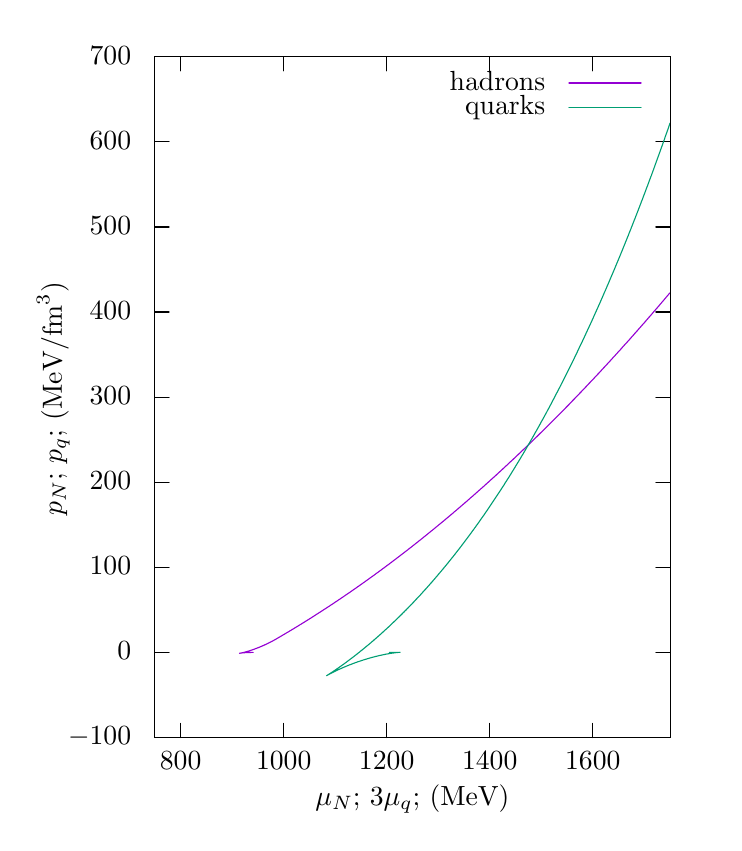
\begin{tikzpicture}[gnuplot]
%% generated with GNUPLOT 5.0p4 (Lua 5.2; terminal rev. 99, script rev. 100)
%% Thu Sep 29 16:33:14 2016
\path (0.000,0.000) rectangle (8.600,10.000);
\gpcolor{color=gp lt color border}
\gpsetlinetype{gp lt border}
\gpsetdashtype{gp dt solid}
\gpsetlinewidth{1.00}
\draw[gp path] (1.504,0.985)--(1.684,0.985);
\draw[gp path] (8.047,0.985)--(7.867,0.985);
\node[gp node right] at (1.320,0.985) {$-100$};
\draw[gp path] (1.504,2.066)--(1.684,2.066);
\draw[gp path] (8.047,2.066)--(7.867,2.066);
\node[gp node right] at (1.320,2.066) {$0$};
\draw[gp path] (1.504,3.147)--(1.684,3.147);
\draw[gp path] (8.047,3.147)--(7.867,3.147);
\node[gp node right] at (1.320,3.147) {$100$};
\draw[gp path] (1.504,4.227)--(1.684,4.227);
\draw[gp path] (8.047,4.227)--(7.867,4.227);
\node[gp node right] at (1.320,4.227) {$200$};
\draw[gp path] (1.504,5.308)--(1.684,5.308);
\draw[gp path] (8.047,5.308)--(7.867,5.308);
\node[gp node right] at (1.320,5.308) {$300$};
\draw[gp path] (1.504,6.389)--(1.684,6.389);
\draw[gp path] (8.047,6.389)--(7.867,6.389);
\node[gp node right] at (1.320,6.389) {$400$};
\draw[gp path] (1.504,7.469)--(1.684,7.469);
\draw[gp path] (8.047,7.469)--(7.867,7.469);
\node[gp node right] at (1.320,7.469) {$500$};
\draw[gp path] (1.504,8.550)--(1.684,8.550);
\draw[gp path] (8.047,8.550)--(7.867,8.550);
\node[gp node right] at (1.320,8.550) {$600$};
\draw[gp path] (1.504,9.631)--(1.684,9.631);
\draw[gp path] (8.047,9.631)--(7.867,9.631);
\node[gp node right] at (1.320,9.631) {$700$};
\draw[gp path] (1.831,0.985)--(1.831,1.165);
\draw[gp path] (1.831,9.631)--(1.831,9.451);
\node[gp node center] at (1.831,0.677) {$800$};
\draw[gp path] (3.140,0.985)--(3.140,1.165);
\draw[gp path] (3.140,9.631)--(3.140,9.451);
\node[gp node center] at (3.140,0.677) {$1000$};
\draw[gp path] (4.448,0.985)--(4.448,1.165);
\draw[gp path] (4.448,9.631)--(4.448,9.451);
\node[gp node center] at (4.448,0.677) {$1200$};
\draw[gp path] (5.757,0.985)--(5.757,1.165);
\draw[gp path] (5.757,9.631)--(5.757,9.451);
\node[gp node center] at (5.757,0.677) {$1400$};
\draw[gp path] (7.066,0.985)--(7.066,1.165);
\draw[gp path] (7.066,9.631)--(7.066,9.451);
\node[gp node center] at (7.066,0.677) {$1600$};
\draw[gp path] (1.504,9.631)--(1.504,0.985)--(8.047,0.985)--(8.047,9.631)--cycle;
\node[gp node center,rotate=-270] at (0.246,5.308) {$p_N$; $p_q$; ($\rm{MeV}/\rm{fm}^3$)};
\node[gp node center] at (4.775,0.215) {$\mu_N$; $3\mu_q$; (MeV)};
\node[gp node right] at (6.579,9.297) {hadrons};
\gpcolor{rgb color={0.580,0.000,0.827}}
\draw[gp path] (6.763,9.297)--(7.679,9.297);
\draw[gp path] (2.728,2.066)--(2.736,2.066)--(2.745,2.066)--(2.753,2.066)--(2.722,2.066)%
  --(2.730,2.066)--(2.738,2.066)--(2.745,2.066)--(2.714,2.065)--(2.722,2.066)--(2.729,2.066)%
  --(2.736,2.066)--(2.744,2.066)--(2.713,2.065)--(2.720,2.065)--(2.727,2.066)--(2.734,2.066)%
  --(2.704,2.065)--(2.711,2.065)--(2.718,2.065)--(2.725,2.066)--(2.694,2.065)--(2.701,2.065)%
  --(2.709,2.065)--(2.716,2.065)--(2.685,2.065)--(2.692,2.065)--(2.699,2.065)--(2.706,2.065)%
  --(2.713,2.065)--(2.683,2.064)--(2.690,2.065)--(2.697,2.065)--(2.704,2.065)--(2.673,2.064)%
  --(2.680,2.064)--(2.688,2.065)--(2.695,2.065)--(2.664,2.064)--(2.671,2.064)--(2.679,2.064)%
  --(2.686,2.065)--(2.693,2.065)--(2.662,2.063)--(2.670,2.064)--(2.677,2.064)--(2.684,2.065)%
  --(2.653,2.063)--(2.661,2.063)--(2.668,2.064)--(2.675,2.064)--(2.645,2.062)--(2.652,2.063)%
  --(2.659,2.063)--(2.667,2.064)--(2.674,2.064)--(2.644,2.062)--(2.651,2.063)--(2.658,2.063)%
  --(2.665,2.064)--(2.635,2.062)--(2.643,2.062)--(2.650,2.063)--(2.657,2.063)--(2.627,2.061)%
  --(2.635,2.062)--(2.642,2.062)--(2.649,2.063)--(2.657,2.063)--(2.627,2.061)--(2.634,2.061)%
  --(2.642,2.062)--(2.649,2.063)--(2.619,2.060)--(2.627,2.061)--(2.634,2.061)--(2.641,2.062)%
  --(2.612,2.060)--(2.619,2.060)--(2.627,2.061)--(2.634,2.061)--(2.642,2.062)--(2.612,2.059)%
  --(2.619,2.060)--(2.627,2.061)--(2.635,2.062)--(2.605,2.059)--(2.613,2.059)--(2.620,2.060)%
  --(2.628,2.061)--(2.598,2.058)--(2.606,2.059)--(2.613,2.060)--(2.621,2.060)--(2.629,2.061)%
  --(2.599,2.058)--(2.607,2.059)--(2.615,2.060)--(2.622,2.061)--(2.593,2.057)--(2.601,2.058)%
  --(2.609,2.059)--(2.616,2.060)--(2.624,2.061)--(2.595,2.057)--(2.603,2.058)--(2.610,2.059)%
  --(2.618,2.060)--(2.589,2.057)--(2.597,2.058)--(2.605,2.059)--(2.612,2.060)--(2.620,2.060)%
  --(2.591,2.057)--(2.599,2.058)--(2.607,2.059)--(2.615,2.060)--(2.586,2.056)--(2.594,2.057)%
  --(2.602,2.058)--(2.610,2.059)--(2.581,2.055)--(2.589,2.056)--(2.597,2.058)--(2.605,2.059)%
  --(2.613,2.060)--(2.584,2.056)--(2.592,2.057)--(2.600,2.058)--(2.608,2.059)--(2.580,2.055)%
  --(2.588,2.056)--(2.596,2.057)--(2.604,2.059)--(2.612,2.060)--(2.583,2.056)--(2.591,2.057)%
  --(2.599,2.058)--(2.607,2.059)--(2.579,2.055)--(2.587,2.056)--(2.595,2.057)--(2.603,2.059)%
  --(2.612,2.060)--(2.583,2.055)--(2.592,2.057)--(2.600,2.058)--(2.608,2.059)--(2.580,2.055)%
  --(2.588,2.056)--(2.596,2.057)--(2.604,2.059)--(2.613,2.060)--(2.585,2.056)--(2.593,2.057)%
  --(2.601,2.058)--(2.609,2.060)--(2.582,2.055)--(2.590,2.056)--(2.598,2.058)--(2.606,2.059)%
  --(2.579,2.054)--(2.587,2.056)--(2.595,2.057)--(2.604,2.059)--(2.612,2.060)--(2.585,2.055)%
  --(2.593,2.057)--(2.601,2.058)--(2.609,2.060)--(2.582,2.055)--(2.591,2.056)--(2.599,2.058)%
  --(2.607,2.060)--(2.616,2.061)--(2.588,2.056)--(2.597,2.058)--(2.605,2.059)--(2.614,2.061)%
  --(2.587,2.056)--(2.595,2.057)--(2.603,2.059)--(2.612,2.061)--(2.620,2.062)--(2.593,2.057)%
  --(2.602,2.059)--(2.610,2.060)--(2.619,2.062)--(2.592,2.056)--(2.600,2.058)--(2.609,2.060)%
  --(2.617,2.062)--(2.626,2.064)--(2.599,2.058)--(2.608,2.060)--(2.616,2.062)--(2.625,2.063)%
  --(2.598,2.058)--(2.607,2.060)--(2.616,2.061)--(2.624,2.063)--(2.598,2.057)--(2.606,2.059)%
  --(2.615,2.061)--(2.624,2.063)--(2.632,2.065)--(2.606,2.059)--(2.615,2.061)--(2.623,2.063)%
  --(2.632,2.065)--(2.606,2.059)--(2.614,2.061)--(2.623,2.063)--(2.632,2.065)--(2.640,2.067)%
  --(2.614,2.061)--(2.623,2.063)--(2.632,2.065)--(2.641,2.067)--(2.615,2.061)--(2.623,2.063)%
  --(2.632,2.065)--(2.641,2.068)--(2.615,2.061)--(2.624,2.063)--(2.633,2.066)--(2.642,2.068)%
  --(2.650,2.070)--(2.625,2.063)--(2.633,2.066)--(2.642,2.068)--(2.651,2.070)--(2.626,2.064)%
  --(2.634,2.066)--(2.643,2.068)--(2.652,2.071)--(2.661,2.073)--(2.636,2.066)--(2.645,2.069)%
  --(2.653,2.071)--(2.662,2.073)--(2.637,2.067)--(2.646,2.069)--(2.655,2.071)--(2.664,2.074)%
  --(2.639,2.067)--(2.648,2.069)--(2.657,2.072)--(2.666,2.074)--(2.675,2.077)--(2.650,2.070)%
  --(2.659,2.072)--(2.668,2.075)--(2.676,2.077)--(2.652,2.070)--(2.661,2.073)--(2.670,2.075)%
  --(2.679,2.078)--(2.654,2.071)--(2.663,2.074)--(2.672,2.076)--(2.681,2.079)--(2.690,2.081)%
  --(2.674,2.077)--(2.683,2.079)--(2.675,2.077)--(2.684,2.080)--(2.677,2.078)--(2.686,2.080)%
  --(2.678,2.078)--(2.687,2.081)--(2.680,2.078)--(2.689,2.081)--(2.681,2.079)--(2.690,2.082)%
  --(2.683,2.079)--(2.692,2.082)--(2.685,2.080)--(2.694,2.083)--(2.703,2.085)--(2.696,2.083)%
  --(2.705,2.086)--(2.697,2.084)--(2.707,2.087)--(2.699,2.084)--(2.708,2.087)--(2.701,2.085)%
  --(2.710,2.088)--(2.703,2.086)--(2.712,2.088)--(2.705,2.086)--(2.714,2.089)--(2.707,2.087)%
  --(2.716,2.090)--(2.709,2.088)--(2.719,2.091)--(2.712,2.088)--(2.721,2.091)--(2.714,2.089)%
  --(2.723,2.092)--(2.716,2.090)--(2.725,2.093)--(2.735,2.096)--(2.728,2.094)--(2.737,2.097)%
  --(2.730,2.094)--(2.739,2.097)--(2.733,2.095)--(2.742,2.098)--(2.735,2.096)--(2.744,2.099)%
  --(2.738,2.097)--(2.747,2.100)--(2.740,2.098)--(2.750,2.101)--(2.743,2.099)--(2.752,2.102)%
  --(2.746,2.100)--(2.755,2.103)--(2.749,2.101)--(2.758,2.104)--(2.752,2.102)--(2.761,2.105)%
  --(2.755,2.103)--(2.764,2.106)--(2.757,2.104)--(2.767,2.107)--(2.761,2.105)--(2.770,2.108)%
  --(2.764,2.106)--(2.773,2.109)--(2.767,2.107)--(2.776,2.111)--(2.770,2.108)--(2.779,2.112)%
  --(2.773,2.110)--(2.783,2.113)--(2.777,2.111)--(2.786,2.114)--(2.780,2.112)--(2.789,2.116)%
  --(2.783,2.113)--(2.793,2.117)--(2.787,2.115)--(2.796,2.118)--(2.790,2.116)--(2.800,2.120)%
  --(2.794,2.117)--(2.803,2.121)--(2.798,2.119)--(2.807,2.122)--(2.801,2.120)--(2.796,2.118)%
  --(2.805,2.122)--(2.800,2.119)--(2.809,2.123)--(2.804,2.121)--(2.813,2.125)--(2.807,2.123)%
  --(2.817,2.126)--(2.811,2.124)--(2.821,2.128)--(2.816,2.126)--(2.825,2.130)--(2.820,2.127)%
  --(2.829,2.131)--(2.824,2.129)--(2.833,2.133)--(2.828,2.131)--(2.823,2.129)--(2.832,2.133)%
  --(2.827,2.130)--(2.837,2.134)--(2.832,2.132)--(2.841,2.136)--(2.836,2.134)--(2.846,2.138)%
  --(2.841,2.136)--(2.850,2.140)--(2.845,2.138)--(2.855,2.142)--(2.850,2.140)--(2.845,2.138)%
  --(2.855,2.142)--(2.850,2.140)--(2.859,2.144)--(2.855,2.142)--(2.864,2.146)--(2.860,2.144)%
  --(2.855,2.142)--(2.865,2.146)--(2.860,2.144)--(2.870,2.148)--(2.865,2.146)--(2.875,2.151)%
  --(2.870,2.149)--(2.880,2.153)--(2.876,2.151)--(2.871,2.149)--(2.881,2.153)--(2.877,2.151)%
  --(2.886,2.156)--(2.882,2.154)--(2.878,2.152)--(2.888,2.156)--(2.884,2.154)--(2.893,2.159)%
  --(2.889,2.157)--(2.899,2.161)--(2.895,2.159)--(2.891,2.158)--(2.901,2.162)--(2.897,2.160)%
  --(2.906,2.165)--(2.903,2.163)--(2.899,2.161)--(2.909,2.166)--(2.905,2.164)--(2.901,2.162)%
  --(2.911,2.167)--(2.908,2.165)--(2.917,2.170)--(2.914,2.168)--(2.910,2.167)--(2.920,2.171)%
  --(2.917,2.170)--(2.926,2.174)--(2.923,2.173)--(2.920,2.171)--(2.930,2.176)--(2.927,2.174)%
  --(2.924,2.173)--(2.933,2.177)--(2.930,2.176)--(2.928,2.175)--(2.937,2.179)--(2.934,2.178)%
  --(2.932,2.177)--(2.941,2.181)--(2.939,2.180)--(2.936,2.179)--(2.946,2.183)--(2.943,2.182)%
  --(2.941,2.181)--(2.950,2.186)--(2.948,2.185)--(2.946,2.184)--(2.956,2.188)--(2.950,2.186)%
  --(2.954,2.188)--(2.958,2.190)--(2.956,2.189)--(2.960,2.190)--(2.958,2.190)--(2.962,2.191)%
  --(2.960,2.191)--(2.964,2.193)--(2.963,2.192)--(2.967,2.194)--(2.971,2.196)--(2.969,2.195)%
  --(2.973,2.197)--(2.972,2.197)--(2.976,2.199)--(2.975,2.198)--(2.974,2.198)--(2.978,2.200)%
  --(2.977,2.199)--(2.981,2.201)--(2.985,2.203)--(2.984,2.203)--(2.988,2.205)--(2.987,2.205)%
  --(2.992,2.207)--(2.996,2.209)--(2.997,2.209)--(3.002,2.212)--(3.003,2.213)--(3.004,2.213)%
  --(3.004,2.214)--(3.005,2.214)--(3.006,2.215)--(3.007,2.215)--(3.008,2.216)--(3.010,2.216)%
  --(3.011,2.217)--(3.013,2.218)--(3.014,2.219)--(3.016,2.220)--(3.018,2.221)--(3.020,2.222)%
  --(3.018,2.221)--(3.020,2.222)--(3.023,2.224)--(3.022,2.223)--(3.024,2.224)--(3.025,2.225)%
  --(3.026,2.225)--(3.027,2.226)--(3.029,2.227)--(3.030,2.228)--(3.031,2.228)--(3.032,2.229)%
  --(3.034,2.230)--(3.036,2.231)--(3.038,2.232)--(3.040,2.233)--(3.041,2.234)--(3.042,2.234)%
  --(3.042,2.235)--(3.043,2.235)--(3.044,2.236)--(3.047,2.237)--(3.056,2.243)--(3.066,2.248)%
  --(3.075,2.254)--(3.084,2.259)--(3.094,2.265)--(3.103,2.270)--(3.113,2.276)--(3.122,2.281)%
  --(3.131,2.287)--(3.141,2.292)--(3.150,2.298)--(3.160,2.303)--(3.169,2.309)--(3.178,2.315)%
  --(3.188,2.320)--(3.197,2.326)--(3.207,2.331)--(3.216,2.337)--(3.225,2.343)--(3.235,2.348)%
  --(3.244,2.354)--(3.254,2.360)--(3.263,2.365)--(3.272,2.371)--(3.282,2.377)--(3.291,2.382)%
  --(3.300,2.388)--(3.310,2.394)--(3.319,2.399)--(3.329,2.405)--(3.338,2.411)--(3.347,2.417)%
  --(3.357,2.422)--(3.366,2.428)--(3.375,2.434)--(3.385,2.440)--(3.394,2.446)--(3.403,2.451)%
  --(3.413,2.457)--(3.422,2.463)--(3.432,2.469)--(3.441,2.475)--(3.450,2.481)--(3.460,2.486)%
  --(3.469,2.492)--(3.478,2.498)--(3.488,2.504)--(3.497,2.510)--(3.506,2.516)--(3.516,2.522)%
  --(3.525,2.528)--(3.534,2.534)--(3.544,2.540)--(3.553,2.546)--(3.562,2.552)--(3.572,2.558)%
  --(3.581,2.564)--(3.590,2.570)--(3.600,2.576)--(3.609,2.582)--(3.618,2.588)--(3.628,2.594)%
  --(3.637,2.600)--(3.646,2.606)--(3.655,2.612)--(3.665,2.618)--(3.674,2.624)--(3.683,2.630)%
  --(3.693,2.636)--(3.702,2.642)--(3.711,2.648)--(3.721,2.654)--(3.730,2.661)--(3.739,2.667)%
  --(3.749,2.673)--(3.758,2.679)--(3.767,2.685)--(3.776,2.691)--(3.786,2.698)--(3.795,2.704)%
  --(3.804,2.710)--(3.814,2.716)--(3.823,2.722)--(3.832,2.729)--(3.841,2.735)--(3.851,2.741)%
  --(3.860,2.747)--(3.869,2.754)--(3.879,2.760)--(3.888,2.766)--(3.897,2.773)--(3.906,2.779)%
  --(3.916,2.785)--(3.925,2.792)--(3.934,2.798)--(3.943,2.804)--(3.953,2.811)--(3.962,2.817)%
  --(3.971,2.823)--(3.981,2.830)--(3.990,2.836)--(3.999,2.843)--(4.008,2.849)--(4.018,2.855)%
  --(4.027,2.862)--(4.036,2.868)--(4.045,2.875)--(4.055,2.881)--(4.064,2.888)--(4.073,2.894)%
  --(4.082,2.901)--(4.092,2.907)--(4.101,2.914)--(4.110,2.920)--(4.119,2.927)--(4.129,2.933)%
  --(4.138,2.940)--(4.147,2.946)--(4.156,2.953)--(4.166,2.959)--(4.175,2.966)--(4.184,2.973)%
  --(4.193,2.979)--(4.203,2.986)--(4.212,2.992)--(4.221,2.999)--(4.230,3.006)--(4.239,3.012)%
  --(4.249,3.019)--(4.258,3.026)--(4.267,3.032)--(4.276,3.039)--(4.286,3.046)--(4.295,3.052)%
  --(4.304,3.059)--(4.313,3.066)--(4.322,3.073)--(4.332,3.079)--(4.341,3.086)--(4.350,3.093)%
  --(4.359,3.100)--(4.369,3.106)--(4.378,3.113)--(4.387,3.120)--(4.396,3.127)--(4.405,3.134)%
  --(4.415,3.140)--(4.424,3.147)--(4.433,3.154)--(4.442,3.161)--(4.451,3.168)--(4.461,3.175)%
  --(4.470,3.181)--(4.479,3.188)--(4.488,3.195)--(4.497,3.202)--(4.507,3.209)--(4.516,3.216)%
  --(4.525,3.223)--(4.534,3.230)--(4.543,3.237)--(4.553,3.244)--(4.562,3.251)--(4.571,3.258)%
  --(4.580,3.265)--(4.589,3.272)--(4.598,3.279)--(4.608,3.286)--(4.617,3.293)--(4.626,3.300)%
  --(4.635,3.307)--(4.644,3.314)--(4.653,3.321)--(4.663,3.328)--(4.672,3.335)--(4.681,3.342)%
  --(4.690,3.349)--(4.699,3.356)--(4.709,3.363)--(4.718,3.371)--(4.727,3.378)--(4.736,3.385)%
  --(4.745,3.392)--(4.754,3.399)--(4.764,3.406)--(4.773,3.414)--(4.782,3.421)--(4.791,3.428)%
  --(4.800,3.435)--(4.809,3.442)--(4.818,3.450)--(4.828,3.457)--(4.837,3.464)--(4.846,3.471)%
  --(4.855,3.479)--(4.864,3.486)--(4.873,3.493)--(4.883,3.500)--(4.892,3.508)--(4.901,3.515)%
  --(4.910,3.522)--(4.919,3.530)--(4.928,3.537)--(4.937,3.544)--(4.947,3.552)--(4.956,3.559)%
  --(4.965,3.567)--(4.974,3.574)--(4.983,3.581)--(4.992,3.589)--(5.001,3.596)--(5.010,3.604)%
  --(5.020,3.611)--(5.029,3.618)--(5.038,3.626)--(5.047,3.633)--(5.056,3.641)--(5.065,3.648)%
  --(5.074,3.656)--(5.084,3.663)--(5.093,3.671)--(5.102,3.678)--(5.111,3.686)--(5.120,3.693)%
  --(5.129,3.701)--(5.138,3.708)--(5.147,3.716)--(5.157,3.724)--(5.166,3.731)--(5.175,3.739)%
  --(5.184,3.746)--(5.193,3.754)--(5.202,3.762)--(5.211,3.769)--(5.220,3.777)--(5.229,3.784)%
  --(5.239,3.792)--(5.248,3.800)--(5.257,3.807)--(5.266,3.815)--(5.275,3.823)--(5.284,3.830)%
  --(5.293,3.838)--(5.302,3.846)--(5.311,3.854)--(5.320,3.861)--(5.330,3.869)--(5.339,3.877)%
  --(5.348,3.885)--(5.357,3.892)--(5.366,3.900)--(5.375,3.908)--(5.384,3.916)--(5.393,3.924)%
  --(5.402,3.931)--(5.411,3.939)--(5.420,3.947)--(5.430,3.955)--(5.439,3.963)--(5.448,3.971)%
  --(5.457,3.978)--(5.466,3.986)--(5.475,3.994)--(5.484,4.002)--(5.493,4.010)--(5.502,4.018)%
  --(5.511,4.026)--(5.520,4.034)--(5.530,4.042)--(5.539,4.050)--(5.548,4.058)--(5.557,4.066)%
  --(5.566,4.074)--(5.575,4.082)--(5.584,4.090)--(5.593,4.098)--(5.602,4.106)--(5.611,4.114)%
  --(5.620,4.122)--(5.629,4.130)--(5.638,4.138)--(5.647,4.146)--(5.657,4.154)--(5.666,4.162)%
  --(5.675,4.170)--(5.684,4.178)--(5.693,4.186)--(5.702,4.195)--(5.711,4.203)--(5.720,4.211)%
  --(5.729,4.219)--(5.738,4.227)--(5.747,4.235)--(5.756,4.243)--(5.765,4.252)--(5.774,4.260)%
  --(5.783,4.268)--(5.792,4.276)--(5.801,4.284)--(5.811,4.293)--(5.820,4.301)--(5.829,4.309)%
  --(5.838,4.317)--(5.847,4.326)--(5.856,4.334)--(5.865,4.342)--(5.874,4.351)--(5.883,4.359)%
  --(5.892,4.367)--(5.901,4.376)--(5.910,4.384)--(5.919,4.392)--(5.928,4.401)--(5.937,4.409)%
  --(5.946,4.417)--(5.955,4.426)--(5.964,4.434)--(5.973,4.442)--(5.982,4.451)--(5.991,4.459)%
  --(6.000,4.468)--(6.009,4.476)--(6.018,4.485)--(6.028,4.493)--(6.037,4.502)--(6.046,4.510)%
  --(6.055,4.518)--(6.064,4.527)--(6.073,4.535)--(6.082,4.544)--(6.091,4.552)--(6.100,4.561)%
  --(6.109,4.570)--(6.118,4.578)--(6.127,4.587)--(6.136,4.595)--(6.145,4.604)--(6.154,4.612)%
  --(6.163,4.621)--(6.172,4.630)--(6.181,4.638)--(6.190,4.647)--(6.199,4.655)--(6.208,4.664)%
  --(6.217,4.673)--(6.226,4.681)--(6.235,4.690)--(6.244,4.699)--(6.253,4.707)--(6.262,4.716)%
  --(6.271,4.725)--(6.280,4.733)--(6.289,4.742)--(6.298,4.751)--(6.307,4.760)--(6.316,4.768)%
  --(6.325,4.777)--(6.334,4.786)--(6.343,4.795)--(6.352,4.803)--(6.361,4.812)--(6.370,4.821)%
  --(6.379,4.830)--(6.388,4.839)--(6.397,4.848)--(6.406,4.856)--(6.415,4.865)--(6.424,4.874)%
  --(6.433,4.883)--(6.442,4.892)--(6.451,4.901)--(6.460,4.910)--(6.469,4.918)--(6.478,4.927)%
  --(6.487,4.936)--(6.496,4.945)--(6.505,4.954)--(6.514,4.963)--(6.523,4.972)--(6.532,4.981)%
  --(6.541,4.990)--(6.550,4.999)--(6.559,5.008)--(6.568,5.017)--(6.577,5.026)--(6.586,5.035)%
  --(6.595,5.044)--(6.604,5.053)--(6.613,5.062)--(6.622,5.071)--(6.631,5.080)--(6.640,5.089)%
  --(6.649,5.098)--(6.658,5.108)--(6.667,5.117)--(6.676,5.126)--(6.685,5.135)--(6.694,5.144)%
  --(6.703,5.153)--(6.712,5.162)--(6.721,5.171)--(6.730,5.181)--(6.739,5.190)--(6.748,5.199)%
  --(6.757,5.208)--(6.766,5.217)--(6.775,5.227)--(6.784,5.236)--(6.792,5.245)--(6.801,5.254)%
  --(6.810,5.264)--(6.819,5.273)--(6.828,5.282)--(6.837,5.291)--(6.846,5.301)--(6.855,5.310)%
  --(6.864,5.319)--(6.873,5.329)--(6.882,5.338)--(6.891,5.347)--(6.900,5.357)--(6.909,5.366)%
  --(6.918,5.375)--(6.927,5.385)--(6.936,5.394)--(6.945,5.403)--(6.954,5.413)--(6.963,5.422)%
  --(6.972,5.432)--(6.981,5.441)--(6.990,5.451)--(6.999,5.460)--(7.008,5.469)--(7.016,5.479)%
  --(7.025,5.488)--(7.034,5.498)--(7.043,5.507)--(7.052,5.517)--(7.061,5.526)--(7.070,5.536)%
  --(7.079,5.545)--(7.088,5.555)--(7.097,5.564)--(7.106,5.574)--(7.115,5.584)--(7.124,5.593)%
  --(7.133,5.603)--(7.142,5.612)--(7.151,5.622)--(7.160,5.632)--(7.169,5.641)--(7.177,5.651)%
  --(7.186,5.660)--(7.195,5.670)--(7.204,5.680)--(7.213,5.689)--(7.222,5.699)--(7.231,5.709)%
  --(7.240,5.718)--(7.249,5.728)--(7.258,5.738)--(7.267,5.748)--(7.276,5.757)--(7.285,5.767)%
  --(7.294,5.777)--(7.303,5.787)--(7.312,5.796)--(7.320,5.806)--(7.329,5.816)--(7.338,5.826)%
  --(7.347,5.835)--(7.356,5.845)--(7.365,5.855)--(7.374,5.865)--(7.383,5.875)--(7.392,5.885)%
  --(7.401,5.894)--(7.410,5.904)--(7.419,5.914)--(7.428,5.924)--(7.436,5.934)--(7.445,5.944)%
  --(7.454,5.954)--(7.463,5.964)--(7.472,5.974)--(7.481,5.984)--(7.490,5.993)--(7.499,6.003)%
  --(7.508,6.013)--(7.517,6.023)--(7.526,6.033)--(7.535,6.043)--(7.544,6.053)--(7.552,6.063)%
  --(7.561,6.073)--(7.570,6.083)--(7.579,6.093)--(7.588,6.103)--(7.597,6.114)--(7.606,6.124)%
  --(7.615,6.134)--(7.624,6.144)--(7.633,6.154)--(7.642,6.164)--(7.650,6.174)--(7.659,6.184)%
  --(7.668,6.194)--(7.677,6.204)--(7.686,6.215)--(7.695,6.225)--(7.704,6.235)--(7.713,6.245)%
  --(7.722,6.255)--(7.731,6.265)--(7.740,6.276)--(7.748,6.286)--(7.757,6.296)--(7.766,6.306)%
  --(7.775,6.317)--(7.784,6.327)--(7.793,6.337)--(7.802,6.347)--(7.811,6.358)--(7.820,6.368)%
  --(7.828,6.378)--(7.837,6.389)--(7.846,6.399)--(7.855,6.409)--(7.864,6.420)--(7.873,6.430)%
  --(7.882,6.440)--(7.891,6.451)--(7.900,6.461)--(7.909,6.471)--(7.917,6.482)--(7.926,6.492)%
  --(7.935,6.502)--(7.944,6.513)--(7.953,6.523)--(7.962,6.534)--(7.971,6.544)--(7.980,6.555)%
  --(7.989,6.565)--(7.997,6.576)--(8.006,6.586)--(8.015,6.597)--(8.024,6.607)--(8.033,6.618)%
  --(8.042,6.628)--(8.047,6.634);
\gpcolor{color=gp lt color border}
\node[gp node right] at (6.579,8.989) {quarks};
\gpcolor{rgb color={0.000,0.620,0.451}}
\draw[gp path] (6.763,8.989)--(7.679,8.989);
\draw[gp path] (4.482,2.066)--(4.515,2.066)--(4.537,2.066)--(4.554,2.066)--(4.566,2.066)%
  --(4.577,2.066)--(4.585,2.067)--(4.593,2.067)--(4.598,2.067)--(4.603,2.067)--(4.607,2.067)%
  --(4.611,2.067)--(4.614,2.067)--(4.616,2.067)--(4.617,2.068)--(4.618,2.068)--(4.619,2.068)%
  --(4.618,2.068)--(4.617,2.067)--(4.616,2.067)--(4.614,2.067)--(4.612,2.067)--(4.610,2.067)%
  --(4.608,2.067)--(4.606,2.067)--(4.603,2.066)--(4.601,2.066)--(4.598,2.066)--(4.595,2.066)%
  --(4.592,2.065)--(4.588,2.065)--(4.585,2.065)--(4.581,2.064)--(4.577,2.064)--(4.573,2.063)%
  --(4.569,2.063)--(4.565,2.063)--(4.561,2.062)--(4.557,2.062)--(4.552,2.061)--(4.548,2.060)%
  --(4.543,2.060)--(4.539,2.059)--(4.534,2.059)--(4.529,2.058)--(4.524,2.057)--(4.519,2.057)%
  --(4.514,2.056)--(4.509,2.055)--(4.504,2.054)--(4.499,2.053)--(4.493,2.053)--(4.488,2.052)%
  --(4.483,2.051)--(4.477,2.050)--(4.472,2.049)--(4.466,2.048)--(4.460,2.047)--(4.455,2.046)%
  --(4.449,2.045)--(4.443,2.044)--(4.437,2.043)--(4.431,2.042)--(4.425,2.040)--(4.419,2.039)%
  --(4.413,2.038)--(4.408,2.037)--(4.402,2.036)--(4.395,2.034)--(4.389,2.033)--(4.383,2.032)%
  --(4.377,2.030)--(4.371,2.029)--(4.364,2.028)--(4.358,2.026)--(4.352,2.025)--(4.345,2.023)%
  --(4.339,2.022)--(4.332,2.020)--(4.326,2.019)--(4.319,2.017)--(4.313,2.015)--(4.306,2.014)%
  --(4.300,2.012)--(4.293,2.010)--(4.287,2.009)--(4.280,2.007)--(4.273,2.005)--(4.267,2.003)%
  --(4.260,2.002)--(4.253,2.000)--(4.247,1.998)--(4.240,1.996)--(4.233,1.994)--(4.227,1.992)%
  --(4.220,1.990)--(4.213,1.988)--(4.206,1.986)--(4.200,1.984)--(4.193,1.982)--(4.186,1.980)%
  --(4.179,1.978)--(4.172,1.976)--(4.166,1.974)--(4.159,1.972)--(4.152,1.970)--(4.145,1.967)%
  --(4.138,1.965)--(4.131,1.963)--(4.125,1.961)--(4.118,1.958)--(4.111,1.956)--(4.104,1.954)%
  --(4.097,1.951)--(4.090,1.949)--(4.083,1.947)--(4.077,1.944)--(4.070,1.942)--(4.063,1.940)%
  --(4.056,1.937)--(4.049,1.935)--(4.043,1.932)--(4.036,1.930)--(4.029,1.927)--(4.022,1.925)%
  --(4.016,1.922)--(4.009,1.920)--(4.002,1.917)--(3.995,1.914)--(3.989,1.912)--(3.982,1.909)%
  --(3.975,1.907)--(3.969,1.904)--(3.962,1.901)--(3.956,1.899)--(3.949,1.896)--(3.943,1.893)%
  --(3.936,1.891)--(3.930,1.888)--(3.923,1.885)--(3.917,1.882)--(3.910,1.880)--(3.904,1.877)%
  --(3.898,1.874)--(3.891,1.872)--(3.885,1.869)--(3.879,1.866)--(3.873,1.863)--(3.867,1.861)%
  --(3.861,1.858)--(3.855,1.855)--(3.849,1.853)--(3.843,1.850)--(3.837,1.847)--(3.831,1.845)%
  --(3.825,1.842)--(3.820,1.839)--(3.814,1.837)--(3.808,1.834)--(3.803,1.831)--(3.798,1.829)%
  --(3.792,1.826)--(3.787,1.824)--(3.782,1.821)--(3.777,1.819)--(3.772,1.816)--(3.767,1.814)%
  --(3.762,1.811)--(3.757,1.809)--(3.753,1.807)--(3.748,1.804)--(3.744,1.802)--(3.740,1.800)%
  --(3.736,1.798)--(3.732,1.796)--(3.728,1.794)--(3.724,1.792)--(3.720,1.790)--(3.717,1.788)%
  --(3.714,1.786)--(3.710,1.785)--(3.707,1.783)--(3.705,1.781)--(3.702,1.780)--(3.699,1.779)%
  --(3.697,1.777)--(3.695,1.776)--(3.693,1.775)--(3.691,1.774)--(3.690,1.773)--(3.688,1.772)%
  --(3.687,1.772)--(3.686,1.771)--(3.685,1.771)--(3.685,1.770)--(3.684,1.770)--(3.685,1.770)%
  --(3.685,1.771)--(3.686,1.771)--(3.687,1.772)--(3.689,1.773)--(3.690,1.773)--(3.692,1.775)%
  --(3.694,1.776)--(3.696,1.777)--(3.698,1.779)--(3.701,1.780)--(3.704,1.782)--(3.707,1.784)%
  --(3.710,1.786)--(3.714,1.788)--(3.718,1.791)--(3.722,1.793)--(3.726,1.796)--(3.730,1.799)%
  --(3.735,1.802)--(3.739,1.805)--(3.744,1.808)--(3.749,1.811)--(3.755,1.815)--(3.760,1.818)%
  --(3.766,1.822)--(3.771,1.826)--(3.777,1.830)--(3.783,1.834)--(3.789,1.838)--(3.796,1.842)%
  --(3.802,1.847)--(3.809,1.851)--(3.815,1.856)--(3.822,1.860)--(3.829,1.865)--(3.836,1.870)%
  --(3.843,1.875)--(3.850,1.880)--(3.857,1.885)--(3.864,1.890)--(3.872,1.895)--(3.879,1.901)%
  --(3.887,1.906)--(3.894,1.911)--(3.902,1.917)--(3.909,1.922)--(3.917,1.928)--(3.925,1.934)%
  --(3.933,1.939)--(3.940,1.945)--(3.948,1.951)--(3.956,1.957)--(3.964,1.963)--(3.972,1.969)%
  --(3.980,1.975)--(3.988,1.981)--(3.996,1.987)--(4.004,1.993)--(4.013,2.000)--(4.021,2.006)%
  --(4.029,2.012)--(4.037,2.018)--(4.045,2.025)--(4.053,2.031)--(4.062,2.038)--(4.070,2.044)%
  --(4.078,2.051)--(4.086,2.057)--(4.095,2.064)--(4.103,2.070)--(4.111,2.077)--(4.119,2.084)%
  --(4.128,2.090)--(4.136,2.097)--(4.144,2.104)--(4.153,2.110)--(4.161,2.117)--(4.169,2.124)%
  --(4.177,2.131)--(4.186,2.138)--(4.194,2.145)--(4.202,2.151)--(4.211,2.158)--(4.219,2.165)%
  --(4.227,2.172)--(4.235,2.179)--(4.244,2.186)--(4.252,2.193)--(4.260,2.200)--(4.268,2.207)%
  --(4.277,2.214)--(4.285,2.221)--(4.293,2.229)--(4.301,2.236)--(4.309,2.243)--(4.318,2.250)%
  --(4.326,2.257)--(4.334,2.264)--(4.342,2.272)--(4.350,2.279)--(4.358,2.286)--(4.367,2.293)%
  --(4.375,2.301)--(4.383,2.308)--(4.391,2.315)--(4.399,2.323)--(4.407,2.330)--(4.415,2.337)%
  --(4.423,2.345)--(4.431,2.352)--(4.439,2.359)--(4.448,2.367)--(4.456,2.374)--(4.464,2.382)%
  --(4.472,2.389)--(4.480,2.396)--(4.488,2.404)--(4.496,2.411)--(4.503,2.419)--(4.511,2.426)%
  --(4.519,2.434)--(4.527,2.442)--(4.535,2.449)--(4.543,2.457)--(4.551,2.464)--(4.559,2.472)%
  --(4.567,2.479)--(4.575,2.487)--(4.582,2.495)--(4.590,2.502)--(4.598,2.510)--(4.606,2.517)%
  --(4.614,2.525)--(4.621,2.533)--(4.629,2.540)--(4.637,2.548)--(4.645,2.556)--(4.652,2.564)%
  --(4.660,2.571)--(4.668,2.579)--(4.676,2.587)--(4.683,2.595)--(4.691,2.602)--(4.699,2.610)%
  --(4.706,2.618)--(4.714,2.626)--(4.722,2.633)--(4.729,2.641)--(4.737,2.649)--(4.744,2.657)%
  --(4.752,2.665)--(4.759,2.673)--(4.767,2.680)--(4.775,2.688)--(4.782,2.696)--(4.790,2.704)%
  --(4.797,2.712)--(4.805,2.720)--(4.812,2.728)--(4.819,2.736)--(4.827,2.744)--(4.834,2.752)%
  --(4.842,2.760)--(4.849,2.768)--(4.857,2.776)--(4.864,2.783)--(4.871,2.791)--(4.879,2.799)%
  --(4.886,2.807)--(4.893,2.816)--(4.901,2.824)--(4.908,2.832)--(4.915,2.840)--(4.923,2.848)%
  --(4.930,2.856)--(4.937,2.864)--(4.945,2.872)--(4.952,2.880)--(4.959,2.888)--(4.966,2.896)%
  --(4.973,2.904)--(4.981,2.912)--(4.988,2.920)--(4.995,2.929)--(5.002,2.937)--(5.009,2.945)%
  --(5.017,2.953)--(5.024,2.961)--(5.031,2.969)--(5.038,2.978)--(5.045,2.986)--(5.052,2.994)%
  --(5.059,3.002)--(5.066,3.010)--(5.073,3.019)--(5.080,3.027)--(5.087,3.035)--(5.094,3.043)%
  --(5.101,3.052)--(5.108,3.060)--(5.115,3.068)--(5.122,3.076)--(5.129,3.085)--(5.136,3.093)%
  --(5.143,3.101)--(5.150,3.110)--(5.157,3.118)--(5.164,3.126)--(5.171,3.135)--(5.178,3.143)%
  --(5.185,3.151)--(5.192,3.160)--(5.198,3.168)--(5.205,3.176)--(5.212,3.185)--(5.219,3.193)%
  --(5.226,3.201)--(5.233,3.210)--(5.239,3.218)--(5.246,3.227)--(5.253,3.235)--(5.260,3.244)%
  --(5.267,3.252)--(5.273,3.260)--(5.280,3.269)--(5.287,3.277)--(5.294,3.286)--(5.300,3.294)%
  --(5.307,3.303)--(5.314,3.311)--(5.320,3.320)--(5.327,3.328)--(5.334,3.337)--(5.340,3.345)%
  --(5.347,3.354)--(5.354,3.362)--(5.360,3.371)--(5.367,3.379)--(5.373,3.388)--(5.380,3.396)%
  --(5.387,3.405)--(5.393,3.414)--(5.400,3.422)--(5.406,3.431)--(5.413,3.439)--(5.419,3.448)%
  --(5.426,3.457)--(5.432,3.465)--(5.439,3.474)--(5.445,3.482)--(5.452,3.491)--(5.458,3.500)%
  --(5.465,3.508)--(5.471,3.517)--(5.478,3.526)--(5.484,3.534)--(5.491,3.543)--(5.497,3.552)%
  --(5.504,3.560)--(5.510,3.569)--(5.516,3.578)--(5.523,3.586)--(5.529,3.595)--(5.535,3.604)%
  --(5.542,3.613)--(5.548,3.621)--(5.555,3.630)--(5.561,3.639)--(5.567,3.648)--(5.574,3.656)%
  --(5.580,3.665)--(5.586,3.674)--(5.592,3.683)--(5.599,3.691)--(5.605,3.700)--(5.611,3.709)%
  --(5.618,3.718)--(5.624,3.727)--(5.630,3.735)--(5.636,3.744)--(5.642,3.753)--(5.649,3.762)%
  --(5.655,3.771)--(5.661,3.780)--(5.667,3.788)--(5.673,3.797)--(5.680,3.806)--(5.686,3.815)%
  --(5.692,3.824)--(5.698,3.833)--(5.704,3.842)--(5.710,3.851)--(5.717,3.859)--(5.723,3.868)%
  --(5.729,3.877)--(5.735,3.886)--(5.741,3.895)--(5.747,3.904)--(5.753,3.913)--(5.759,3.922)%
  --(5.765,3.931)--(5.771,3.940)--(5.777,3.949)--(5.783,3.958)--(5.789,3.967)--(5.795,3.976)%
  --(5.801,3.985)--(5.807,3.994)--(5.813,4.003)--(5.819,4.012)--(5.825,4.021)--(5.831,4.030)%
  --(5.837,4.039)--(5.843,4.048)--(5.849,4.057)--(5.855,4.066)--(5.861,4.075)--(5.867,4.084)%
  --(5.873,4.093)--(5.879,4.102)--(5.885,4.111)--(5.891,4.120)--(5.897,4.129)--(5.903,4.139)%
  --(5.908,4.148)--(5.914,4.157)--(5.920,4.166)--(5.926,4.175)--(5.932,4.184)--(5.938,4.193)%
  --(5.944,4.202)--(5.949,4.212)--(5.955,4.221)--(5.961,4.230)--(5.967,4.239)--(5.973,4.248)%
  --(5.978,4.257)--(5.984,4.266)--(5.990,4.276)--(5.996,4.285)--(6.002,4.294)--(6.007,4.303)%
  --(6.013,4.312)--(6.019,4.322)--(6.025,4.331)--(6.030,4.340)--(6.036,4.349)--(6.042,4.359)%
  --(6.047,4.368)--(6.053,4.377)--(6.059,4.386)--(6.065,4.396)--(6.070,4.405)--(6.076,4.414)%
  --(6.082,4.423)--(6.087,4.433)--(6.093,4.442)--(6.099,4.451)--(6.104,4.461)--(6.110,4.470)%
  --(6.115,4.479)--(6.121,4.488)--(6.127,4.498)--(6.132,4.507)--(6.138,4.516)--(6.144,4.526)%
  --(6.149,4.535)--(6.155,4.544)--(6.160,4.554)--(6.166,4.563)--(6.171,4.573)--(6.177,4.582)%
  --(6.183,4.591)--(6.188,4.601)--(6.194,4.610)--(6.199,4.619)--(6.205,4.629)--(6.210,4.638)%
  --(6.216,4.648)--(6.221,4.657)--(6.227,4.666)--(6.232,4.676)--(6.238,4.685)--(6.243,4.695)%
  --(6.249,4.704)--(6.254,4.714)--(6.260,4.723)--(6.265,4.733)--(6.270,4.742)--(6.276,4.751)%
  --(6.281,4.761)--(6.287,4.770)--(6.292,4.780)--(6.298,4.789)--(6.303,4.799)--(6.308,4.808)%
  --(6.314,4.818)--(6.319,4.827)--(6.325,4.837)--(6.330,4.846)--(6.335,4.856)--(6.341,4.866)%
  --(6.346,4.875)--(6.352,4.885)--(6.357,4.894)--(6.362,4.904)--(6.368,4.913)--(6.373,4.923)%
  --(6.378,4.932)--(6.384,4.942)--(6.389,4.952)--(6.394,4.961)--(6.400,4.971)--(6.405,4.980)%
  --(6.410,4.990)--(6.415,5.000)--(6.421,5.009)--(6.426,5.019)--(6.431,5.028)--(6.437,5.038)%
  --(6.442,5.048)--(6.447,5.057)--(6.452,5.067)--(6.458,5.077)--(6.463,5.086)--(6.468,5.096)%
  --(6.473,5.106)--(6.479,5.115)--(6.484,5.125)--(6.489,5.135)--(6.494,5.144)--(6.499,5.154)%
  --(6.505,5.164)--(6.510,5.173)--(6.515,5.183)--(6.520,5.193)--(6.525,5.203)--(6.531,5.212)%
  --(6.536,5.222)--(6.541,5.232)--(6.546,5.241)--(6.551,5.251)--(6.556,5.261)--(6.561,5.271)%
  --(6.567,5.280)--(6.572,5.290)--(6.577,5.300)--(6.582,5.310)--(6.587,5.320)--(6.592,5.329)%
  --(6.597,5.339)--(6.602,5.349)--(6.607,5.359)--(6.613,5.369)--(6.618,5.378)--(6.623,5.388)%
  --(6.628,5.398)--(6.633,5.408)--(6.638,5.418)--(6.643,5.427)--(6.648,5.437)--(6.653,5.447)%
  --(6.658,5.457)--(6.663,5.467)--(6.668,5.477)--(6.673,5.487)--(6.678,5.496)--(6.683,5.506)%
  --(6.688,5.516)--(6.693,5.526)--(6.698,5.536)--(6.703,5.546)--(6.708,5.556)--(6.713,5.566)%
  --(6.718,5.576)--(6.723,5.586)--(6.728,5.595)--(6.733,5.605)--(6.738,5.615)--(6.743,5.625)%
  --(6.748,5.635)--(6.753,5.645)--(6.758,5.655)--(6.763,5.665)--(6.768,5.675)--(6.773,5.685)%
  --(6.778,5.695)--(6.783,5.705)--(6.788,5.715)--(6.792,5.725)--(6.797,5.735)--(6.802,5.745)%
  --(6.807,5.755)--(6.812,5.765)--(6.817,5.775)--(6.822,5.785)--(6.827,5.795)--(6.832,5.805)%
  --(6.836,5.815)--(6.841,5.825)--(6.846,5.835)--(6.851,5.845)--(6.856,5.855)--(6.861,5.865)%
  --(6.866,5.875)--(6.870,5.885)--(6.875,5.895)--(6.880,5.905)--(6.885,5.915)--(6.890,5.925)%
  --(6.894,5.936)--(6.899,5.946)--(6.904,5.956)--(6.909,5.966)--(6.914,5.976)--(6.918,5.986)%
  --(6.923,5.996)--(6.928,6.006)--(6.933,6.016)--(6.938,6.027)--(6.942,6.037)--(6.947,6.047)%
  --(6.952,6.057)--(6.957,6.067)--(6.961,6.077)--(6.966,6.087)--(6.971,6.098)--(6.976,6.108)%
  --(6.980,6.118)--(6.985,6.128)--(6.990,6.138)--(6.995,6.148)--(6.999,6.159)--(7.004,6.169)%
  --(7.009,6.179)--(7.013,6.189)--(7.018,6.199)--(7.023,6.210)--(7.027,6.220)--(7.032,6.230)%
  --(7.037,6.240)--(7.042,6.251)--(7.046,6.261)--(7.051,6.271)--(7.056,6.281)--(7.060,6.291)%
  --(7.065,6.302)--(7.070,6.312)--(7.074,6.322)--(7.079,6.333)--(7.083,6.343)--(7.088,6.353)%
  --(7.093,6.363)--(7.097,6.374)--(7.102,6.384)--(7.107,6.394)--(7.111,6.405)--(7.116,6.415)%
  --(7.120,6.425)--(7.125,6.435)--(7.130,6.446)--(7.134,6.456)--(7.139,6.466)--(7.143,6.477)%
  --(7.148,6.487)--(7.153,6.497)--(7.157,6.508)--(7.162,6.518)--(7.166,6.528)--(7.171,6.539)%
  --(7.175,6.549)--(7.180,6.560)--(7.185,6.570)--(7.189,6.580)--(7.194,6.591)--(7.198,6.601)%
  --(7.203,6.611)--(7.207,6.622)--(7.212,6.632)--(7.216,6.643)--(7.221,6.653)--(7.225,6.663)%
  --(7.230,6.674)--(7.234,6.684)--(7.239,6.695)--(7.243,6.705)--(7.248,6.716)--(7.252,6.726)%
  --(7.257,6.736)--(7.261,6.747)--(7.266,6.757)--(7.270,6.768)--(7.275,6.778)--(7.279,6.789)%
  --(7.284,6.799)--(7.288,6.810)--(7.293,6.820)--(7.297,6.831)--(7.302,6.841)--(7.306,6.852)%
  --(7.311,6.862)--(7.315,6.873)--(7.319,6.883)--(7.324,6.894)--(7.328,6.904)--(7.333,6.915)%
  --(7.337,6.925)--(7.342,6.936)--(7.346,6.946)--(7.350,6.957)--(7.355,6.967)--(7.359,6.978)%
  --(7.364,6.988)--(7.368,6.999)--(7.372,7.009)--(7.377,7.020)--(7.381,7.031)--(7.386,7.041)%
  --(7.390,7.052)--(7.394,7.062)--(7.399,7.073)--(7.403,7.083)--(7.408,7.094)--(7.412,7.105)%
  --(7.416,7.115)--(7.421,7.126)--(7.425,7.136)--(7.429,7.147)--(7.434,7.158)--(7.438,7.168)%
  --(7.442,7.179)--(7.447,7.190)--(7.451,7.200)--(7.455,7.211)--(7.460,7.222)--(7.464,7.232)%
  --(7.468,7.243)--(7.473,7.253)--(7.477,7.264)--(7.481,7.275)--(7.486,7.285)--(7.490,7.296)%
  --(7.494,7.307)--(7.498,7.317)--(7.503,7.328)--(7.507,7.339)--(7.511,7.350)--(7.516,7.360)%
  --(7.520,7.371)--(7.524,7.382)--(7.528,7.392)--(7.533,7.403)--(7.537,7.414)--(7.541,7.425)%
  --(7.546,7.435)--(7.550,7.446)--(7.554,7.457)--(7.558,7.467)--(7.563,7.478)--(7.567,7.489)%
  --(7.571,7.500)--(7.575,7.510)--(7.579,7.521)--(7.584,7.532)--(7.588,7.543)--(7.592,7.554)%
  --(7.596,7.564)--(7.601,7.575)--(7.605,7.586)--(7.609,7.597)--(7.613,7.607)--(7.617,7.618)%
  --(7.622,7.629)--(7.626,7.640)--(7.630,7.651)--(7.634,7.661)--(7.638,7.672)--(7.643,7.683)%
  --(7.647,7.694)--(7.651,7.705)--(7.655,7.716)--(7.659,7.726)--(7.663,7.737)--(7.668,7.748)%
  --(7.672,7.759)--(7.676,7.770)--(7.680,7.781)--(7.684,7.792)--(7.688,7.802)--(7.693,7.813)%
  --(7.697,7.824)--(7.701,7.835)--(7.705,7.846)--(7.709,7.857)--(7.713,7.868)--(7.717,7.879)%
  --(7.722,7.890)--(7.726,7.900)--(7.730,7.911)--(7.734,7.922)--(7.738,7.933)--(7.742,7.944)%
  --(7.746,7.955)--(7.750,7.966)--(7.754,7.977)--(7.759,7.988)--(7.763,7.999)--(7.767,8.010)%
  --(7.771,8.021)--(7.775,8.032)--(7.779,8.043)--(7.783,8.054)--(7.787,8.064)--(7.791,8.075)%
  --(7.795,8.086)--(7.799,8.097)--(7.803,8.108)--(7.808,8.119)--(7.812,8.130)--(7.816,8.141)%
  --(7.820,8.152)--(7.824,8.163)--(7.828,8.174)--(7.832,8.185)--(7.836,8.196)--(7.840,8.207)%
  --(7.844,8.218)--(7.848,8.229)--(7.852,8.240)--(7.856,8.251)--(7.860,8.263)--(7.864,8.274)%
  --(7.868,8.285)--(7.872,8.296)--(7.876,8.307)--(7.880,8.318)--(7.884,8.329)--(7.888,8.340)%
  --(7.892,8.351)--(7.896,8.362)--(7.900,8.373)--(7.904,8.384)--(7.908,8.395)--(7.912,8.406)%
  --(7.916,8.417)--(7.920,8.429)--(7.924,8.440)--(7.928,8.451)--(7.932,8.462)--(7.936,8.473)%
  --(7.940,8.484)--(7.944,8.495)--(7.948,8.506)--(7.952,8.517)--(7.956,8.529)--(7.960,8.540)%
  --(7.964,8.551)--(7.968,8.562)--(7.972,8.573)--(7.976,8.584)--(7.980,8.595)--(7.983,8.607)%
  --(7.987,8.618)--(7.991,8.629)--(7.995,8.640)--(7.999,8.651)--(8.003,8.662)--(8.007,8.674)%
  --(8.011,8.685)--(8.015,8.696)--(8.019,8.707)--(8.023,8.718)--(8.027,8.730)--(8.031,8.741)%
  --(8.034,8.752)--(8.038,8.763)--(8.042,8.774)--(8.046,8.786)--(8.047,8.788);
\gpcolor{color=gp lt color border}
\draw[gp path] (1.504,9.631)--(1.504,0.985)--(8.047,0.985)--(8.047,9.631)--cycle;
%% coordinates of the plot area
\gpdefrectangularnode{gp plot 1}{\pgfpoint{1.504cm}{0.985cm}}{\pgfpoint{8.047cm}{9.631cm}}
\end{tikzpicture}
%% gnuplot variables

	\caption{BuballaR\_2-eNJL1OmegaRho1}
\end{figure}
\begin{figure}
	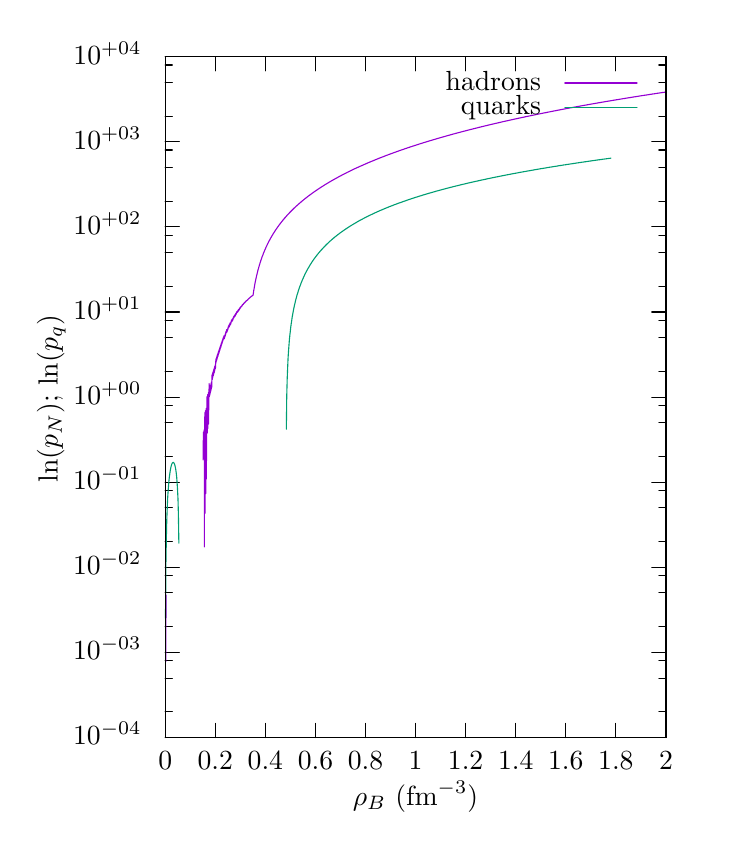
\begin{tikzpicture}[gnuplot]
%% generated with GNUPLOT 5.0p4 (Lua 5.2; terminal rev. 99, script rev. 100)
%% Thu Sep 29 16:33:14 2016
\path (0.000,0.000) rectangle (8.600,10.000);
\gpcolor{color=gp lt color border}
\gpsetlinetype{gp lt border}
\gpsetdashtype{gp dt solid}
\gpsetlinewidth{1.00}
\draw[gp path] (1.688,0.985)--(1.868,0.985);
\draw[gp path] (8.047,0.985)--(7.867,0.985);
\node[gp node right] at (1.504,0.985) {$10^{-04}$};
\draw[gp path] (1.688,1.310)--(1.778,1.310);
\draw[gp path] (8.047,1.310)--(7.957,1.310);
\draw[gp path] (1.688,1.740)--(1.778,1.740);
\draw[gp path] (8.047,1.740)--(7.957,1.740);
\draw[gp path] (1.688,1.961)--(1.778,1.961);
\draw[gp path] (8.047,1.961)--(7.957,1.961);
\draw[gp path] (1.688,2.066)--(1.868,2.066);
\draw[gp path] (8.047,2.066)--(7.867,2.066);
\node[gp node right] at (1.504,2.066) {$10^{-03}$};
\draw[gp path] (1.688,2.391)--(1.778,2.391);
\draw[gp path] (8.047,2.391)--(7.957,2.391);
\draw[gp path] (1.688,2.821)--(1.778,2.821);
\draw[gp path] (8.047,2.821)--(7.957,2.821);
\draw[gp path] (1.688,3.042)--(1.778,3.042);
\draw[gp path] (8.047,3.042)--(7.957,3.042);
\draw[gp path] (1.688,3.147)--(1.868,3.147);
\draw[gp path] (8.047,3.147)--(7.867,3.147);
\node[gp node right] at (1.504,3.147) {$10^{-02}$};
\draw[gp path] (1.688,3.472)--(1.778,3.472);
\draw[gp path] (8.047,3.472)--(7.957,3.472);
\draw[gp path] (1.688,3.902)--(1.778,3.902);
\draw[gp path] (8.047,3.902)--(7.957,3.902);
\draw[gp path] (1.688,4.123)--(1.778,4.123);
\draw[gp path] (8.047,4.123)--(7.957,4.123);
\draw[gp path] (1.688,4.227)--(1.868,4.227);
\draw[gp path] (8.047,4.227)--(7.867,4.227);
\node[gp node right] at (1.504,4.227) {$10^{-01}$};
\draw[gp path] (1.688,4.553)--(1.778,4.553);
\draw[gp path] (8.047,4.553)--(7.957,4.553);
\draw[gp path] (1.688,4.983)--(1.778,4.983);
\draw[gp path] (8.047,4.983)--(7.957,4.983);
\draw[gp path] (1.688,5.203)--(1.778,5.203);
\draw[gp path] (8.047,5.203)--(7.957,5.203);
\draw[gp path] (1.688,5.308)--(1.868,5.308);
\draw[gp path] (8.047,5.308)--(7.867,5.308);
\node[gp node right] at (1.504,5.308) {$10^{+00}$};
\draw[gp path] (1.688,5.633)--(1.778,5.633);
\draw[gp path] (8.047,5.633)--(7.957,5.633);
\draw[gp path] (1.688,6.063)--(1.778,6.063);
\draw[gp path] (8.047,6.063)--(7.957,6.063);
\draw[gp path] (1.688,6.284)--(1.778,6.284);
\draw[gp path] (8.047,6.284)--(7.957,6.284);
\draw[gp path] (1.688,6.389)--(1.868,6.389);
\draw[gp path] (8.047,6.389)--(7.867,6.389);
\node[gp node right] at (1.504,6.389) {$10^{+01}$};
\draw[gp path] (1.688,6.714)--(1.778,6.714);
\draw[gp path] (8.047,6.714)--(7.957,6.714);
\draw[gp path] (1.688,7.144)--(1.778,7.144);
\draw[gp path] (8.047,7.144)--(7.957,7.144);
\draw[gp path] (1.688,7.365)--(1.778,7.365);
\draw[gp path] (8.047,7.365)--(7.957,7.365);
\draw[gp path] (1.688,7.470)--(1.868,7.470);
\draw[gp path] (8.047,7.470)--(7.867,7.470);
\node[gp node right] at (1.504,7.470) {$10^{+02}$};
\draw[gp path] (1.688,7.795)--(1.778,7.795);
\draw[gp path] (8.047,7.795)--(7.957,7.795);
\draw[gp path] (1.688,8.225)--(1.778,8.225);
\draw[gp path] (8.047,8.225)--(7.957,8.225);
\draw[gp path] (1.688,8.446)--(1.778,8.446);
\draw[gp path] (8.047,8.446)--(7.957,8.446);
\draw[gp path] (1.688,8.550)--(1.868,8.550);
\draw[gp path] (8.047,8.550)--(7.867,8.550);
\node[gp node right] at (1.504,8.550) {$10^{+03}$};
\draw[gp path] (1.688,8.876)--(1.778,8.876);
\draw[gp path] (8.047,8.876)--(7.957,8.876);
\draw[gp path] (1.688,9.306)--(1.778,9.306);
\draw[gp path] (8.047,9.306)--(7.957,9.306);
\draw[gp path] (1.688,9.526)--(1.778,9.526);
\draw[gp path] (8.047,9.526)--(7.957,9.526);
\draw[gp path] (1.688,9.631)--(1.868,9.631);
\draw[gp path] (8.047,9.631)--(7.867,9.631);
\node[gp node right] at (1.504,9.631) {$10^{+04}$};
\draw[gp path] (1.688,0.985)--(1.688,1.165);
\draw[gp path] (1.688,9.631)--(1.688,9.451);
\node[gp node center] at (1.688,0.677) {$0$};
\draw[gp path] (2.324,0.985)--(2.324,1.165);
\draw[gp path] (2.324,9.631)--(2.324,9.451);
\node[gp node center] at (2.324,0.677) {$0.2$};
\draw[gp path] (2.960,0.985)--(2.960,1.165);
\draw[gp path] (2.960,9.631)--(2.960,9.451);
\node[gp node center] at (2.960,0.677) {$0.4$};
\draw[gp path] (3.596,0.985)--(3.596,1.165);
\draw[gp path] (3.596,9.631)--(3.596,9.451);
\node[gp node center] at (3.596,0.677) {$0.6$};
\draw[gp path] (4.232,0.985)--(4.232,1.165);
\draw[gp path] (4.232,9.631)--(4.232,9.451);
\node[gp node center] at (4.232,0.677) {$0.8$};
\draw[gp path] (4.868,0.985)--(4.868,1.165);
\draw[gp path] (4.868,9.631)--(4.868,9.451);
\node[gp node center] at (4.868,0.677) {$1$};
\draw[gp path] (5.503,0.985)--(5.503,1.165);
\draw[gp path] (5.503,9.631)--(5.503,9.451);
\node[gp node center] at (5.503,0.677) {$1.2$};
\draw[gp path] (6.139,0.985)--(6.139,1.165);
\draw[gp path] (6.139,9.631)--(6.139,9.451);
\node[gp node center] at (6.139,0.677) {$1.4$};
\draw[gp path] (6.775,0.985)--(6.775,1.165);
\draw[gp path] (6.775,9.631)--(6.775,9.451);
\node[gp node center] at (6.775,0.677) {$1.6$};
\draw[gp path] (7.411,0.985)--(7.411,1.165);
\draw[gp path] (7.411,9.631)--(7.411,9.451);
\node[gp node center] at (7.411,0.677) {$1.8$};
\draw[gp path] (8.047,0.985)--(8.047,1.165);
\draw[gp path] (8.047,9.631)--(8.047,9.451);
\node[gp node center] at (8.047,0.677) {$2$};
\draw[gp path] (1.688,9.631)--(1.688,0.985)--(8.047,0.985)--(8.047,9.631)--cycle;
\node[gp node center,rotate=-270] at (0.246,5.308) {$\ln(p_N)$; $\ln(p_q)$};
\node[gp node center] at (4.867,0.215) {$\rho_B$ ($\rm{fm}^{-3}$)};
\node[gp node right] at (6.579,9.297) {hadrons};
\gpcolor{rgb color={0.580,0.000,0.827}}
\draw[gp path] (6.763,9.297)--(7.679,9.297);
\draw[gp path] (1.695,1.949)--(1.698,2.796);
\draw[gp path] (2.170,4.510)--(2.172,4.863);
\draw[gp path] (2.179,4.561)--(2.181,4.893);
\draw[gp path] (2.185,3.406)--(2.187,4.616)--(2.189,4.925)--(2.191,5.111)--(2.193,3.832)%
  --(2.196,4.673)--(2.198,4.959)--(2.200,5.137)--(2.202,4.083)--(2.204,4.732)--(2.206,4.996)%
  --(2.208,5.165)--(2.210,4.268)--(2.213,4.792)--(2.215,5.034)--(2.217,5.195)--(2.219,5.315)%
  --(2.221,4.851)--(2.223,5.074)--(2.225,5.225)--(2.227,5.340)--(2.229,4.909)--(2.232,5.114)%
  --(2.234,5.257)--(2.236,5.367)--(2.238,4.967)--(2.240,5.155)--(2.242,5.289)--(2.244,5.394)%
  --(2.246,5.481)--(2.249,5.314)--(2.251,5.415)--(2.253,5.331)--(2.255,5.430)--(2.257,5.347)%
  --(2.259,5.444)--(2.261,5.364)--(2.263,5.458)--(2.266,5.381)--(2.268,5.473)--(2.270,5.398)%
  --(2.272,5.488)--(2.274,5.415)--(2.276,5.502)--(2.278,5.432)--(2.280,5.517)--(2.282,5.589)%
  --(2.285,5.532)--(2.287,5.603)--(2.289,5.547)--(2.291,5.616)--(2.293,5.562)--(2.295,5.629)%
  --(2.297,5.577)--(2.299,5.643)--(2.302,5.591)--(2.304,5.656)--(2.306,5.606)--(2.308,5.670)%
  --(2.310,5.621)--(2.312,5.683)--(2.314,5.636)--(2.316,5.697)--(2.318,5.651)--(2.321,5.710)%
  --(2.323,5.666)--(2.325,5.724)--(2.327,5.681)--(2.329,5.738)--(2.331,5.788)--(2.333,5.751)%
  --(2.335,5.801)--(2.338,5.765)--(2.340,5.814)--(2.342,5.778)--(2.344,5.826)--(2.346,5.792)%
  --(2.348,5.839)--(2.350,5.805)--(2.352,5.851)--(2.355,5.819)--(2.357,5.864)--(2.359,5.832)%
  --(2.361,5.876)--(2.363,5.846)--(2.365,5.889)--(2.367,5.859)--(2.369,5.901)--(2.371,5.872)%
  --(2.374,5.914)--(2.376,5.886)--(2.378,5.926)--(2.380,5.899)--(2.382,5.939)--(2.384,5.912)%
  --(2.386,5.951)--(2.388,5.925)--(2.391,5.964)--(2.393,5.939)--(2.395,5.976)--(2.397,5.952)%
  --(2.399,5.988)--(2.401,5.965)--(2.403,6.001)--(2.405,5.978)--(2.408,6.013)--(2.410,5.991)%
  --(2.412,6.025)--(2.414,6.004)--(2.416,6.037)--(2.418,6.016)--(2.420,6.050)--(2.422,6.029)%
  --(2.424,6.062)--(2.427,6.042)--(2.429,6.074)--(2.431,6.054)--(2.433,6.086)--(2.435,6.067)%
  --(2.437,6.048)--(2.439,6.080)--(2.441,6.061)--(2.444,6.092)--(2.446,6.074)--(2.448,6.104)%
  --(2.450,6.087)--(2.452,6.117)--(2.454,6.100)--(2.456,6.129)--(2.458,6.112)--(2.460,6.141)%
  --(2.463,6.125)--(2.465,6.153)--(2.467,6.138)--(2.469,6.166)--(2.471,6.150)--(2.473,6.135)%
  --(2.475,6.163)--(2.477,6.148)--(2.480,6.175)--(2.482,6.161)--(2.484,6.188)--(2.486,6.174)%
  --(2.488,6.200)--(2.490,6.186)--(2.492,6.212)--(2.494,6.199)--(2.497,6.224)--(2.499,6.212)%
  --(2.501,6.199)--(2.503,6.224)--(2.505,6.212)--(2.507,6.236)--(2.509,6.224)--(2.511,6.249)%
  --(2.513,6.237)--(2.516,6.225)--(2.518,6.250)--(2.520,6.238)--(2.522,6.262)--(2.524,6.251)%
  --(2.526,6.275)--(2.528,6.264)--(2.530,6.287)--(2.533,6.277)--(2.535,6.266)--(2.537,6.289)%
  --(2.539,6.279)--(2.541,6.302)--(2.543,6.292)--(2.545,6.282)--(2.547,6.305)--(2.550,6.296)%
  --(2.552,6.318)--(2.554,6.309)--(2.556,6.330)--(2.558,6.322)--(2.560,6.313)--(2.562,6.335)%
  --(2.564,6.326)--(2.566,6.347)--(2.569,6.339)--(2.571,6.331)--(2.573,6.352)--(2.575,6.344)%
  --(2.577,6.337)--(2.579,6.358)--(2.581,6.350)--(2.583,6.371)--(2.586,6.363)--(2.588,6.356)%
  --(2.590,6.377)--(2.592,6.370)--(2.594,6.390)--(2.596,6.383)--(2.598,6.377)--(2.600,6.397)%
  --(2.602,6.390)--(2.605,6.384)--(2.607,6.404)--(2.609,6.398)--(2.611,6.392)--(2.613,6.412)%
  --(2.615,6.406)--(2.617,6.401)--(2.619,6.420)--(2.622,6.415)--(2.624,6.410)--(2.626,6.429)%
  --(2.628,6.424)--(2.630,6.419)--(2.632,6.438)--(2.634,6.434)--(2.636,6.429)--(2.639,6.448)%
  --(2.641,6.438)--(2.643,6.445)--(2.645,6.452)--(2.647,6.449)--(2.649,6.456)--(2.651,6.452)%
  --(2.653,6.460)--(2.655,6.456)--(2.658,6.464)--(2.660,6.461)--(2.662,6.468)--(2.664,6.476)%
  --(2.666,6.473)--(2.668,6.481)--(2.670,6.478)--(2.672,6.486)--(2.675,6.484)--(2.677,6.482)%
  --(2.679,6.489)--(2.681,6.488)--(2.683,6.496)--(2.685,6.494)--(2.687,6.502)--(2.689,6.501)%
  --(2.691,6.500)--(2.694,6.508)--(2.696,6.507)--(2.698,6.506)--(2.700,6.514)--(2.702,6.514)%
  --(2.704,6.514)--(2.706,6.522)--(2.708,6.522)--(2.711,6.522)--(2.713,6.522)--(2.715,6.531)%
  --(2.717,6.532)--(2.719,6.532)--(2.721,6.533)--(2.723,6.534)--(2.725,6.536)--(2.728,6.537)%
  --(2.730,6.539)--(2.732,6.541)--(2.734,6.543)--(2.736,6.545)--(2.738,6.547)--(2.740,6.550)%
  --(2.742,6.552)--(2.744,6.555)--(2.747,6.558)--(2.749,6.561)--(2.751,6.559)--(2.753,6.562)%
  --(2.755,6.566)--(2.757,6.565)--(2.759,6.569)--(2.761,6.569)--(2.764,6.571)--(2.766,6.574)%
  --(2.768,6.577)--(2.770,6.577)--(2.772,6.578)--(2.774,6.580)--(2.776,6.582)--(2.778,6.584)%
  --(2.781,6.585)--(2.783,6.588)--(2.785,6.588)--(2.787,6.591)--(2.789,6.591)--(2.791,6.594)%
  --(2.793,6.595)--(2.795,6.597)--(2.797,6.598)--(2.800,6.600)--(2.802,6.601)--(2.804,6.605)%
  --(2.806,6.620)--(2.808,6.634)--(2.810,6.648)--(2.812,6.662)--(2.814,6.675)--(2.817,6.688)%
  --(2.819,6.700)--(2.821,6.712)--(2.823,6.724)--(2.825,6.736)--(2.827,6.747)--(2.829,6.759)%
  --(2.831,6.769)--(2.833,6.780)--(2.836,6.791)--(2.838,6.801)--(2.840,6.811)--(2.842,6.821)%
  --(2.844,6.830)--(2.846,6.840)--(2.848,6.849)--(2.850,6.858)--(2.853,6.867)--(2.855,6.876)%
  --(2.857,6.885)--(2.859,6.893)--(2.861,6.902)--(2.863,6.910)--(2.865,6.918)--(2.867,6.926)%
  --(2.870,6.934)--(2.872,6.942)--(2.874,6.949)--(2.876,6.957)--(2.878,6.964)--(2.880,6.971)%
  --(2.882,6.979)--(2.884,6.986)--(2.886,6.993)--(2.889,7.000)--(2.891,7.007)--(2.893,7.013)%
  --(2.895,7.020)--(2.897,7.027)--(2.899,7.033)--(2.901,7.040)--(2.903,7.046)--(2.906,7.052)%
  --(2.908,7.058)--(2.910,7.065)--(2.912,7.071)--(2.914,7.077)--(2.916,7.083)--(2.918,7.088)%
  --(2.920,7.094)--(2.923,7.100)--(2.925,7.106)--(2.927,7.111)--(2.929,7.117)--(2.931,7.122)%
  --(2.933,7.128)--(2.935,7.133)--(2.937,7.139)--(2.939,7.144)--(2.942,7.149)--(2.944,7.154)%
  --(2.946,7.159)--(2.948,7.164)--(2.950,7.170)--(2.952,7.175)--(2.954,7.179)--(2.956,7.184)%
  --(2.959,7.189)--(2.961,7.194)--(2.963,7.199)--(2.965,7.204)--(2.967,7.208)--(2.969,7.213)%
  --(2.971,7.218)--(2.973,7.222)--(2.975,7.227)--(2.978,7.231)--(2.980,7.236)--(2.982,7.240)%
  --(2.984,7.245)--(2.986,7.249)--(2.988,7.253)--(2.990,7.258)--(2.992,7.262)--(2.995,7.266)%
  --(2.997,7.270)--(2.999,7.274)--(3.001,7.279)--(3.003,7.283)--(3.005,7.287)--(3.007,7.291)%
  --(3.009,7.295)--(3.012,7.299)--(3.014,7.303)--(3.016,7.307)--(3.018,7.311)--(3.020,7.315)%
  --(3.022,7.318)--(3.024,7.322)--(3.026,7.326)--(3.028,7.330)--(3.031,7.334)--(3.033,7.337)%
  --(3.035,7.341)--(3.037,7.345)--(3.039,7.348)--(3.041,7.352)--(3.043,7.356)--(3.045,7.359)%
  --(3.048,7.363)--(3.050,7.366)--(3.052,7.370)--(3.054,7.373)--(3.056,7.377)--(3.058,7.380)%
  --(3.060,7.384)--(3.062,7.387)--(3.064,7.391)--(3.067,7.394)--(3.069,7.397)--(3.071,7.401)%
  --(3.073,7.404)--(3.075,7.407)--(3.077,7.411)--(3.079,7.414)--(3.081,7.417)--(3.084,7.420)%
  --(3.086,7.424)--(3.088,7.427)--(3.090,7.430)--(3.092,7.433)--(3.094,7.436)--(3.096,7.439)%
  --(3.098,7.442)--(3.101,7.446)--(3.103,7.449)--(3.105,7.452)--(3.107,7.455)--(3.109,7.458)%
  --(3.111,7.461)--(3.113,7.464)--(3.115,7.467)--(3.117,7.470)--(3.120,7.473)--(3.122,7.476)%
  --(3.124,7.479)--(3.126,7.482)--(3.128,7.484)--(3.130,7.487)--(3.132,7.490)--(3.134,7.493)%
  --(3.137,7.496)--(3.139,7.499)--(3.141,7.502)--(3.143,7.504)--(3.145,7.507)--(3.147,7.510)%
  --(3.149,7.513)--(3.151,7.515)--(3.154,7.518)--(3.156,7.521)--(3.158,7.524)--(3.160,7.526)%
  --(3.162,7.529)--(3.164,7.532)--(3.166,7.534)--(3.168,7.537)--(3.170,7.540)--(3.173,7.542)%
  --(3.175,7.545)--(3.177,7.548)--(3.179,7.550)--(3.181,7.553)--(3.183,7.555)--(3.185,7.558)%
  --(3.187,7.561)--(3.190,7.563)--(3.192,7.566)--(3.194,7.568)--(3.196,7.571)--(3.198,7.573)%
  --(3.200,7.576)--(3.202,7.578)--(3.204,7.581)--(3.206,7.583)--(3.209,7.586)--(3.211,7.588)%
  --(3.213,7.590)--(3.215,7.593)--(3.217,7.595)--(3.219,7.598)--(3.221,7.600)--(3.223,7.602)%
  --(3.226,7.605)--(3.228,7.607)--(3.230,7.610)--(3.232,7.612)--(3.234,7.614)--(3.236,7.617)%
  --(3.238,7.619)--(3.240,7.621)--(3.243,7.624)--(3.245,7.626)--(3.247,7.628)--(3.249,7.630)%
  --(3.251,7.633)--(3.253,7.635)--(3.255,7.637)--(3.257,7.640)--(3.259,7.642)--(3.262,7.644)%
  --(3.264,7.646)--(3.266,7.648)--(3.268,7.651)--(3.270,7.653)--(3.272,7.655)--(3.274,7.657)%
  --(3.276,7.659)--(3.279,7.662)--(3.281,7.664)--(3.283,7.666)--(3.285,7.668)--(3.287,7.670)%
  --(3.289,7.672)--(3.291,7.675)--(3.293,7.677)--(3.295,7.679)--(3.298,7.681)--(3.300,7.683)%
  --(3.302,7.685)--(3.304,7.687)--(3.306,7.689)--(3.308,7.691)--(3.310,7.693)--(3.312,7.696)%
  --(3.315,7.698)--(3.317,7.700)--(3.319,7.702)--(3.321,7.704)--(3.323,7.706)--(3.325,7.708)%
  --(3.327,7.710)--(3.329,7.712)--(3.332,7.714)--(3.334,7.716)--(3.336,7.718)--(3.338,7.720)%
  --(3.340,7.722)--(3.342,7.724)--(3.344,7.726)--(3.346,7.728)--(3.348,7.730)--(3.351,7.732)%
  --(3.353,7.734)--(3.355,7.736)--(3.357,7.737)--(3.359,7.739)--(3.361,7.741)--(3.363,7.743)%
  --(3.365,7.745)--(3.368,7.747)--(3.370,7.749)--(3.372,7.751)--(3.374,7.753)--(3.376,7.755)%
  --(3.378,7.756)--(3.380,7.758)--(3.382,7.760)--(3.385,7.762)--(3.387,7.764)--(3.389,7.766)%
  --(3.391,7.768)--(3.393,7.770)--(3.395,7.771)--(3.397,7.773)--(3.399,7.775)--(3.401,7.777)%
  --(3.404,7.779)--(3.406,7.780)--(3.408,7.782)--(3.410,7.784)--(3.412,7.786)--(3.414,7.788)%
  --(3.416,7.789)--(3.418,7.791)--(3.421,7.793)--(3.423,7.795)--(3.425,7.797)--(3.427,7.798)%
  --(3.429,7.800)--(3.431,7.802)--(3.433,7.804)--(3.435,7.805)--(3.437,7.807)--(3.440,7.809)%
  --(3.442,7.811)--(3.444,7.812)--(3.446,7.814)--(3.448,7.816)--(3.450,7.817)--(3.452,7.819)%
  --(3.454,7.821)--(3.457,7.823)--(3.459,7.824)--(3.461,7.826)--(3.463,7.828)--(3.465,7.829)%
  --(3.467,7.831)--(3.469,7.833)--(3.471,7.834)--(3.474,7.836)--(3.476,7.838)--(3.478,7.839)%
  --(3.480,7.841)--(3.482,7.843)--(3.484,7.844)--(3.486,7.846)--(3.488,7.848)--(3.490,7.849)%
  --(3.493,7.851)--(3.495,7.853)--(3.497,7.854)--(3.499,7.856)--(3.501,7.857)--(3.503,7.859)%
  --(3.505,7.861)--(3.507,7.862)--(3.510,7.864)--(3.512,7.865)--(3.514,7.867)--(3.516,7.869)%
  --(3.518,7.870)--(3.520,7.872)--(3.522,7.873)--(3.524,7.875)--(3.527,7.877)--(3.529,7.878)%
  --(3.531,7.880)--(3.533,7.881)--(3.535,7.883)--(3.537,7.884)--(3.539,7.886)--(3.541,7.887)%
  --(3.543,7.889)--(3.546,7.891)--(3.548,7.892)--(3.550,7.894)--(3.552,7.895)--(3.554,7.897)%
  --(3.556,7.898)--(3.558,7.900)--(3.560,7.901)--(3.563,7.903)--(3.565,7.904)--(3.567,7.906)%
  --(3.569,7.907)--(3.571,7.909)--(3.573,7.910)--(3.575,7.912)--(3.577,7.913)--(3.579,7.915)%
  --(3.582,7.916)--(3.584,7.918)--(3.586,7.919)--(3.588,7.921)--(3.590,7.922)--(3.592,7.924)%
  --(3.594,7.925)--(3.596,7.927)--(3.599,7.928)--(3.601,7.929)--(3.603,7.931)--(3.605,7.932)%
  --(3.607,7.934)--(3.609,7.935)--(3.611,7.937)--(3.613,7.938)--(3.616,7.940)--(3.618,7.941)%
  --(3.620,7.942)--(3.622,7.944)--(3.624,7.945)--(3.626,7.947)--(3.628,7.948)--(3.630,7.950)%
  --(3.632,7.951)--(3.635,7.952)--(3.637,7.954)--(3.639,7.955)--(3.641,7.957)--(3.643,7.958)%
  --(3.645,7.959)--(3.647,7.961)--(3.649,7.962)--(3.652,7.964)--(3.654,7.965)--(3.656,7.966)%
  --(3.658,7.968)--(3.660,7.969)--(3.662,7.970)--(3.664,7.972)--(3.666,7.973)--(3.668,7.975)%
  --(3.671,7.976)--(3.673,7.977)--(3.675,7.979)--(3.677,7.980)--(3.679,7.981)--(3.681,7.983)%
  --(3.683,7.984)--(3.685,7.985)--(3.688,7.987)--(3.690,7.988)--(3.692,7.989)--(3.694,7.991)%
  --(3.696,7.992)--(3.698,7.993)--(3.700,7.995)--(3.702,7.996)--(3.705,7.997)--(3.707,7.999)%
  --(3.709,8.000)--(3.711,8.001)--(3.713,8.003)--(3.715,8.004)--(3.717,8.005)--(3.719,8.007)%
  --(3.721,8.008)--(3.724,8.009)--(3.726,8.011)--(3.728,8.012)--(3.730,8.013)--(3.732,8.014)%
  --(3.734,8.016)--(3.736,8.017)--(3.738,8.018)--(3.741,8.020)--(3.743,8.021)--(3.745,8.022)%
  --(3.747,8.023)--(3.749,8.025)--(3.751,8.026)--(3.753,8.027)--(3.755,8.029)--(3.758,8.030)%
  --(3.760,8.031)--(3.762,8.032)--(3.764,8.034)--(3.766,8.035)--(3.768,8.036)--(3.770,8.037)%
  --(3.772,8.039)--(3.774,8.040)--(3.777,8.041)--(3.779,8.042)--(3.781,8.044)--(3.783,8.045)%
  --(3.785,8.046)--(3.787,8.047)--(3.789,8.049)--(3.791,8.050)--(3.794,8.051)--(3.796,8.052)%
  --(3.798,8.053)--(3.800,8.055)--(3.802,8.056)--(3.804,8.057)--(3.806,8.058)--(3.808,8.060)%
  --(3.810,8.061)--(3.813,8.062)--(3.815,8.063)--(3.817,8.064)--(3.819,8.066)--(3.821,8.067)%
  --(3.823,8.068)--(3.825,8.069)--(3.827,8.070)--(3.830,8.072)--(3.832,8.073)--(3.834,8.074)%
  --(3.836,8.075)--(3.838,8.076)--(3.840,8.078)--(3.842,8.079)--(3.844,8.080)--(3.847,8.081)%
  --(3.849,8.082)--(3.851,8.083)--(3.853,8.085)--(3.855,8.086)--(3.857,8.087)--(3.859,8.088)%
  --(3.861,8.089)--(3.863,8.090)--(3.866,8.092)--(3.868,8.093)--(3.870,8.094)--(3.872,8.095)%
  --(3.874,8.096)--(3.876,8.097)--(3.878,8.099)--(3.880,8.100)--(3.883,8.101)--(3.885,8.102)%
  --(3.887,8.103)--(3.889,8.104)--(3.891,8.105)--(3.893,8.107)--(3.895,8.108)--(3.897,8.109)%
  --(3.900,8.110)--(3.902,8.111)--(3.904,8.112)--(3.906,8.113)--(3.908,8.115)--(3.910,8.116)%
  --(3.912,8.117)--(3.914,8.118)--(3.916,8.119)--(3.919,8.120)--(3.921,8.121)--(3.923,8.122)%
  --(3.925,8.124)--(3.927,8.125)--(3.929,8.126)--(3.931,8.127)--(3.933,8.128)--(3.936,8.129)%
  --(3.938,8.130)--(3.940,8.131)--(3.942,8.132)--(3.944,8.133)--(3.946,8.135)--(3.948,8.136)%
  --(3.950,8.137)--(3.952,8.138)--(3.955,8.139)--(3.957,8.140)--(3.959,8.141)--(3.961,8.142)%
  --(3.963,8.143)--(3.965,8.144)--(3.967,8.145)--(3.969,8.147)--(3.972,8.148)--(3.974,8.149)%
  --(3.976,8.150)--(3.978,8.151)--(3.980,8.152)--(3.982,8.153)--(3.984,8.154)--(3.986,8.155)%
  --(3.989,8.156)--(3.991,8.157)--(3.993,8.158)--(3.995,8.159)--(3.997,8.160)--(3.999,8.162)%
  --(4.001,8.163)--(4.003,8.164)--(4.005,8.165)--(4.008,8.166)--(4.010,8.167)--(4.012,8.168)%
  --(4.014,8.169)--(4.016,8.170)--(4.018,8.171)--(4.020,8.172)--(4.022,8.173)--(4.025,8.174)%
  --(4.027,8.175)--(4.029,8.176)--(4.031,8.177)--(4.033,8.178)--(4.035,8.179)--(4.037,8.180)%
  --(4.039,8.181)--(4.041,8.182)--(4.044,8.183)--(4.046,8.184)--(4.048,8.186)--(4.050,8.187)%
  --(4.052,8.188)--(4.054,8.189)--(4.056,8.190)--(4.058,8.191)--(4.061,8.192)--(4.063,8.193)%
  --(4.065,8.194)--(4.067,8.195)--(4.069,8.196)--(4.071,8.197)--(4.073,8.198)--(4.075,8.199)%
  --(4.078,8.200)--(4.080,8.201)--(4.082,8.202)--(4.084,8.203)--(4.086,8.204)--(4.088,8.205)%
  --(4.090,8.206)--(4.092,8.207)--(4.094,8.208)--(4.097,8.209)--(4.099,8.210)--(4.101,8.211)%
  --(4.103,8.212)--(4.105,8.213)--(4.107,8.214)--(4.109,8.215)--(4.111,8.216)--(4.114,8.217)%
  --(4.116,8.218)--(4.118,8.219)--(4.120,8.220)--(4.122,8.221)--(4.124,8.222)--(4.126,8.223)%
  --(4.128,8.224)--(4.131,8.225)--(4.133,8.225)--(4.135,8.226)--(4.137,8.227)--(4.139,8.228)%
  --(4.141,8.229)--(4.143,8.230)--(4.145,8.231)--(4.147,8.232)--(4.150,8.233)--(4.152,8.234)%
  --(4.154,8.235)--(4.156,8.236)--(4.158,8.237)--(4.160,8.238)--(4.162,8.239)--(4.164,8.240)%
  --(4.167,8.241)--(4.169,8.242)--(4.171,8.243)--(4.173,8.244)--(4.175,8.245)--(4.177,8.246)%
  --(4.179,8.247)--(4.181,8.248)--(4.183,8.249)--(4.186,8.249)--(4.188,8.250)--(4.190,8.251)%
  --(4.192,8.252)--(4.194,8.253)--(4.196,8.254)--(4.198,8.255)--(4.200,8.256)--(4.203,8.257)%
  --(4.205,8.258)--(4.207,8.259)--(4.209,8.260)--(4.211,8.261)--(4.213,8.262)--(4.215,8.263)%
  --(4.217,8.264)--(4.220,8.264)--(4.222,8.265)--(4.224,8.266)--(4.226,8.267)--(4.228,8.268)%
  --(4.230,8.269)--(4.232,8.270)--(4.234,8.271)--(4.236,8.272)--(4.239,8.273)--(4.241,8.274)%
  --(4.243,8.275)--(4.245,8.275)--(4.247,8.276)--(4.249,8.277)--(4.251,8.278)--(4.253,8.279)%
  --(4.256,8.280)--(4.258,8.281)--(4.260,8.282)--(4.262,8.283)--(4.264,8.284)--(4.266,8.285)%
  --(4.268,8.285)--(4.270,8.286)--(4.273,8.287)--(4.275,8.288)--(4.277,8.289)--(4.279,8.290)%
  --(4.281,8.291)--(4.283,8.292)--(4.285,8.293)--(4.287,8.294)--(4.289,8.294)--(4.292,8.295)%
  --(4.294,8.296)--(4.296,8.297)--(4.298,8.298)--(4.300,8.299)--(4.302,8.300)--(4.304,8.301)%
  --(4.306,8.302)--(4.309,8.302)--(4.311,8.303)--(4.313,8.304)--(4.315,8.305)--(4.317,8.306)%
  --(4.319,8.307)--(4.321,8.308)--(4.323,8.309)--(4.325,8.309)--(4.328,8.310)--(4.330,8.311)%
  --(4.332,8.312)--(4.334,8.313)--(4.336,8.314)--(4.338,8.315)--(4.340,8.316)--(4.342,8.316)%
  --(4.345,8.317)--(4.347,8.318)--(4.349,8.319)--(4.351,8.320)--(4.353,8.321)--(4.355,8.322)%
  --(4.357,8.322)--(4.359,8.323)--(4.362,8.324)--(4.364,8.325)--(4.366,8.326)--(4.368,8.327)%
  --(4.370,8.328)--(4.372,8.328)--(4.374,8.329)--(4.376,8.330)--(4.378,8.331)--(4.381,8.332)%
  --(4.383,8.333)--(4.385,8.334)--(4.387,8.334)--(4.389,8.335)--(4.391,8.336)--(4.393,8.337)%
  --(4.395,8.338)--(4.398,8.339)--(4.400,8.339)--(4.402,8.340)--(4.404,8.341)--(4.406,8.342)%
  --(4.408,8.343)--(4.410,8.344)--(4.412,8.345)--(4.414,8.345)--(4.417,8.346)--(4.419,8.347)%
  --(4.421,8.348)--(4.423,8.349)--(4.425,8.350)--(4.427,8.350)--(4.429,8.351)--(4.431,8.352)%
  --(4.434,8.353)--(4.436,8.354)--(4.438,8.355)--(4.440,8.355)--(4.442,8.356)--(4.444,8.357)%
  --(4.446,8.358)--(4.448,8.359)--(4.451,8.359)--(4.453,8.360)--(4.455,8.361)--(4.457,8.362)%
  --(4.459,8.363)--(4.461,8.364)--(4.463,8.364)--(4.465,8.365)--(4.467,8.366)--(4.470,8.367)%
  --(4.472,8.368)--(4.474,8.368)--(4.476,8.369)--(4.478,8.370)--(4.480,8.371)--(4.482,8.372)%
  --(4.484,8.372)--(4.487,8.373)--(4.489,8.374)--(4.491,8.375)--(4.493,8.376)--(4.495,8.377)%
  --(4.497,8.377)--(4.499,8.378)--(4.501,8.379)--(4.504,8.380)--(4.506,8.381)--(4.508,8.381)%
  --(4.510,8.382)--(4.512,8.383)--(4.514,8.384)--(4.516,8.385)--(4.518,8.385)--(4.520,8.386)%
  --(4.523,8.387)--(4.525,8.388)--(4.527,8.388)--(4.529,8.389)--(4.531,8.390)--(4.533,8.391)%
  --(4.535,8.392)--(4.537,8.392)--(4.540,8.393)--(4.542,8.394)--(4.544,8.395)--(4.546,8.396)%
  --(4.548,8.396)--(4.550,8.397)--(4.552,8.398)--(4.554,8.399)--(4.556,8.400)--(4.559,8.400)%
  --(4.561,8.401)--(4.563,8.402)--(4.565,8.403)--(4.567,8.403)--(4.569,8.404)--(4.571,8.405)%
  --(4.573,8.406)--(4.576,8.407)--(4.578,8.407)--(4.580,8.408)--(4.582,8.409)--(4.584,8.410)%
  --(4.586,8.410)--(4.588,8.411)--(4.590,8.412)--(4.593,8.413)--(4.595,8.413)--(4.597,8.414)%
  --(4.599,8.415)--(4.601,8.416)--(4.603,8.417)--(4.605,8.417)--(4.607,8.418)--(4.609,8.419)%
  --(4.612,8.420)--(4.614,8.420)--(4.616,8.421)--(4.618,8.422)--(4.620,8.423)--(4.622,8.423)%
  --(4.624,8.424)--(4.626,8.425)--(4.629,8.426)--(4.631,8.426)--(4.633,8.427)--(4.635,8.428)%
  --(4.637,8.429)--(4.639,8.429)--(4.641,8.430)--(4.643,8.431)--(4.646,8.432)--(4.648,8.432)%
  --(4.650,8.433)--(4.652,8.434)--(4.654,8.435)--(4.656,8.435)--(4.658,8.436)--(4.660,8.437)%
  --(4.662,8.438)--(4.665,8.438)--(4.667,8.439)--(4.669,8.440)--(4.671,8.441)--(4.673,8.441)%
  --(4.675,8.442)--(4.677,8.443)--(4.679,8.444)--(4.682,8.444)--(4.684,8.445)--(4.686,8.446)%
  --(4.688,8.447)--(4.690,8.447)--(4.692,8.448)--(4.694,8.449)--(4.696,8.450)--(4.698,8.450)%
  --(4.701,8.451)--(4.703,8.452)--(4.705,8.452)--(4.707,8.453)--(4.709,8.454)--(4.711,8.455)%
  --(4.713,8.455)--(4.715,8.456)--(4.718,8.457)--(4.720,8.458)--(4.722,8.458)--(4.724,8.459)%
  --(4.726,8.460)--(4.728,8.460)--(4.730,8.461)--(4.732,8.462)--(4.735,8.463)--(4.737,8.463)%
  --(4.739,8.464)--(4.741,8.465)--(4.743,8.466)--(4.745,8.466)--(4.747,8.467)--(4.749,8.468)%
  --(4.751,8.468)--(4.754,8.469)--(4.756,8.470)--(4.758,8.471)--(4.760,8.471)--(4.762,8.472)%
  --(4.764,8.473)--(4.766,8.473)--(4.768,8.474)--(4.771,8.475)--(4.773,8.476)--(4.775,8.476)%
  --(4.777,8.477)--(4.779,8.478)--(4.781,8.478)--(4.783,8.479)--(4.785,8.480)--(4.787,8.481)%
  --(4.790,8.481)--(4.792,8.482)--(4.794,8.483)--(4.796,8.483)--(4.798,8.484)--(4.800,8.485)%
  --(4.802,8.485)--(4.804,8.486)--(4.807,8.487)--(4.809,8.488)--(4.811,8.488)--(4.813,8.489)%
  --(4.815,8.490)--(4.817,8.490)--(4.819,8.491)--(4.821,8.492)--(4.824,8.492)--(4.826,8.493)%
  --(4.828,8.494)--(4.830,8.495)--(4.832,8.495)--(4.834,8.496)--(4.836,8.497)--(4.838,8.497)%
  --(4.840,8.498)--(4.843,8.499)--(4.845,8.499)--(4.847,8.500)--(4.849,8.501)--(4.851,8.501)%
  --(4.853,8.502)--(4.855,8.503)--(4.857,8.504)--(4.860,8.504)--(4.862,8.505)--(4.864,8.506)%
  --(4.866,8.506)--(4.868,8.507)--(4.870,8.508)--(4.872,8.508)--(4.874,8.509)--(4.877,8.510)%
  --(4.879,8.510)--(4.881,8.511)--(4.883,8.512)--(4.885,8.512)--(4.887,8.513)--(4.889,8.514)%
  --(4.891,8.514)--(4.893,8.515)--(4.896,8.516)--(4.898,8.516)--(4.900,8.517)--(4.902,8.518)%
  --(4.904,8.519)--(4.906,8.519)--(4.908,8.520)--(4.910,8.521)--(4.913,8.521)--(4.915,8.522)%
  --(4.917,8.523)--(4.919,8.523)--(4.921,8.524)--(4.923,8.525)--(4.925,8.525)--(4.927,8.526)%
  --(4.929,8.527)--(4.932,8.527)--(4.934,8.528)--(4.936,8.529)--(4.938,8.529)--(4.940,8.530)%
  --(4.942,8.531)--(4.944,8.531)--(4.946,8.532)--(4.949,8.533)--(4.951,8.533)--(4.953,8.534)%
  --(4.955,8.535)--(4.957,8.535)--(4.959,8.536)--(4.961,8.537)--(4.963,8.537)--(4.966,8.538)%
  --(4.968,8.539)--(4.970,8.539)--(4.972,8.540)--(4.974,8.541)--(4.976,8.541)--(4.978,8.542)%
  --(4.980,8.543)--(4.982,8.543)--(4.985,8.544)--(4.987,8.544)--(4.989,8.545)--(4.991,8.546)%
  --(4.993,8.546)--(4.995,8.547)--(4.997,8.548)--(4.999,8.548)--(5.002,8.549)--(5.004,8.550)%
  --(5.006,8.550)--(5.008,8.551)--(5.010,8.552)--(5.012,8.552)--(5.014,8.553)--(5.016,8.554)%
  --(5.019,8.554)--(5.021,8.555)--(5.023,8.556)--(5.025,8.556)--(5.027,8.557)--(5.029,8.557)%
  --(5.031,8.558)--(5.033,8.559)--(5.035,8.559)--(5.038,8.560)--(5.040,8.561)--(5.042,8.561)%
  --(5.044,8.562)--(5.046,8.563)--(5.048,8.563)--(5.050,8.564)--(5.052,8.565)--(5.055,8.565)%
  --(5.057,8.566)--(5.059,8.566)--(5.061,8.567)--(5.063,8.568)--(5.065,8.568)--(5.067,8.569)%
  --(5.069,8.570)--(5.071,8.570)--(5.074,8.571)--(5.076,8.572)--(5.078,8.572)--(5.080,8.573)%
  --(5.082,8.573)--(5.084,8.574)--(5.086,8.575)--(5.088,8.575)--(5.091,8.576)--(5.093,8.577)%
  --(5.095,8.577)--(5.097,8.578)--(5.099,8.578)--(5.101,8.579)--(5.103,8.580)--(5.105,8.580)%
  --(5.108,8.581)--(5.110,8.582)--(5.112,8.582)--(5.114,8.583)--(5.116,8.583)--(5.118,8.584)%
  --(5.120,8.585)--(5.122,8.585)--(5.124,8.586)--(5.127,8.587)--(5.129,8.587)--(5.131,8.588)%
  --(5.133,8.588)--(5.135,8.589)--(5.137,8.590)--(5.139,8.590)--(5.141,8.591)--(5.144,8.592)%
  --(5.146,8.592)--(5.148,8.593)--(5.150,8.593)--(5.152,8.594)--(5.154,8.595)--(5.156,8.595)%
  --(5.158,8.596)--(5.160,8.597)--(5.163,8.597)--(5.165,8.598)--(5.167,8.598)--(5.169,8.599)%
  --(5.171,8.600)--(5.173,8.600)--(5.175,8.601)--(5.177,8.601)--(5.180,8.602)--(5.182,8.603)%
  --(5.184,8.603)--(5.186,8.604)--(5.188,8.604)--(5.190,8.605)--(5.192,8.606)--(5.194,8.606)%
  --(5.197,8.607)--(5.199,8.608)--(5.201,8.608)--(5.203,8.609)--(5.205,8.609)--(5.207,8.610)%
  --(5.209,8.611)--(5.211,8.611)--(5.213,8.612)--(5.216,8.612)--(5.218,8.613)--(5.220,8.614)%
  --(5.222,8.614)--(5.224,8.615)--(5.226,8.615)--(5.228,8.616)--(5.230,8.617)--(5.233,8.617)%
  --(5.235,8.618)--(5.237,8.618)--(5.239,8.619)--(5.241,8.620)--(5.243,8.620)--(5.245,8.621)%
  --(5.247,8.621)--(5.250,8.622)--(5.252,8.623)--(5.254,8.623)--(5.256,8.624)--(5.258,8.624)%
  --(5.260,8.625)--(5.262,8.626)--(5.264,8.626)--(5.266,8.627)--(5.269,8.627)--(5.271,8.628)%
  --(5.273,8.629)--(5.275,8.629)--(5.277,8.630)--(5.279,8.630)--(5.281,8.631)--(5.283,8.631)%
  --(5.286,8.632)--(5.288,8.633)--(5.290,8.633)--(5.292,8.634)--(5.294,8.634)--(5.296,8.635)%
  --(5.298,8.636)--(5.300,8.636)--(5.302,8.637)--(5.305,8.637)--(5.307,8.638)--(5.309,8.639)%
  --(5.311,8.639)--(5.313,8.640)--(5.315,8.640)--(5.317,8.641)--(5.319,8.641)--(5.322,8.642)%
  --(5.324,8.643)--(5.326,8.643)--(5.328,8.644)--(5.330,8.644)--(5.332,8.645)--(5.334,8.646)%
  --(5.336,8.646)--(5.339,8.647)--(5.341,8.647)--(5.343,8.648)--(5.345,8.648)--(5.347,8.649)%
  --(5.349,8.650)--(5.351,8.650)--(5.353,8.651)--(5.355,8.651)--(5.358,8.652)--(5.360,8.652)%
  --(5.362,8.653)--(5.364,8.654)--(5.366,8.654)--(5.368,8.655)--(5.370,8.655)--(5.372,8.656)%
  --(5.375,8.656)--(5.377,8.657)--(5.379,8.658)--(5.381,8.658)--(5.383,8.659)--(5.385,8.659)%
  --(5.387,8.660)--(5.389,8.660)--(5.392,8.661)--(5.394,8.662)--(5.396,8.662)--(5.398,8.663)%
  --(5.400,8.663)--(5.402,8.664)--(5.404,8.664)--(5.406,8.665)--(5.408,8.666)--(5.411,8.666)%
  --(5.413,8.667)--(5.415,8.667)--(5.417,8.668)--(5.419,8.668)--(5.421,8.669)--(5.423,8.670)%
  --(5.425,8.670)--(5.428,8.671)--(5.430,8.671)--(5.432,8.672)--(5.434,8.672)--(5.436,8.673)%
  --(5.438,8.674)--(5.440,8.674)--(5.442,8.675)--(5.444,8.675)--(5.447,8.676)--(5.449,8.676)%
  --(5.451,8.677)--(5.453,8.677)--(5.455,8.678)--(5.457,8.679)--(5.459,8.679)--(5.461,8.680)%
  --(5.464,8.680)--(5.466,8.681)--(5.468,8.681)--(5.470,8.682)--(5.472,8.682)--(5.474,8.683)%
  --(5.476,8.684)--(5.478,8.684)--(5.481,8.685)--(5.483,8.685)--(5.485,8.686)--(5.487,8.686)%
  --(5.489,8.687)--(5.491,8.687)--(5.493,8.688)--(5.495,8.689)--(5.497,8.689)--(5.500,8.690)%
  --(5.502,8.690)--(5.504,8.691)--(5.506,8.691)--(5.508,8.692)--(5.510,8.692)--(5.512,8.693)%
  --(5.514,8.693)--(5.517,8.694)--(5.519,8.695)--(5.521,8.695)--(5.523,8.696)--(5.525,8.696)%
  --(5.527,8.697)--(5.529,8.697)--(5.531,8.698)--(5.533,8.698)--(5.536,8.699)--(5.538,8.700)%
  --(5.540,8.700)--(5.542,8.701)--(5.544,8.701)--(5.546,8.702)--(5.548,8.702)--(5.550,8.703)%
  --(5.553,8.703)--(5.555,8.704)--(5.557,8.704)--(5.559,8.705)--(5.561,8.705)--(5.563,8.706)%
  --(5.565,8.707)--(5.567,8.707)--(5.570,8.708)--(5.572,8.708)--(5.574,8.709)--(5.576,8.709)%
  --(5.578,8.710)--(5.580,8.710)--(5.582,8.711)--(5.584,8.711)--(5.586,8.712)--(5.589,8.712)%
  --(5.591,8.713)--(5.593,8.714)--(5.595,8.714)--(5.597,8.715)--(5.599,8.715)--(5.601,8.716)%
  --(5.603,8.716)--(5.606,8.717)--(5.608,8.717)--(5.610,8.718)--(5.612,8.718)--(5.614,8.719)%
  --(5.616,8.719)--(5.618,8.720)--(5.620,8.721)--(5.623,8.721)--(5.625,8.722)--(5.627,8.722)%
  --(5.629,8.723)--(5.631,8.723)--(5.633,8.724)--(5.635,8.724)--(5.637,8.725)--(5.639,8.725)%
  --(5.642,8.726)--(5.644,8.726)--(5.646,8.727)--(5.648,8.727)--(5.650,8.728)--(5.652,8.728)%
  --(5.654,8.729)--(5.656,8.729)--(5.659,8.730)--(5.661,8.731)--(5.663,8.731)--(5.665,8.732)%
  --(5.667,8.732)--(5.669,8.733)--(5.671,8.733)--(5.673,8.734)--(5.675,8.734)--(5.678,8.735)%
  --(5.680,8.735)--(5.682,8.736)--(5.684,8.736)--(5.686,8.737)--(5.688,8.737)--(5.690,8.738)%
  --(5.692,8.738)--(5.695,8.739)--(5.697,8.739)--(5.699,8.740)--(5.701,8.740)--(5.703,8.741)%
  --(5.705,8.742)--(5.707,8.742)--(5.709,8.743)--(5.712,8.743)--(5.714,8.744)--(5.716,8.744)%
  --(5.718,8.745)--(5.720,8.745)--(5.722,8.746)--(5.724,8.746)--(5.726,8.747)--(5.728,8.747)%
  --(5.731,8.748)--(5.733,8.748)--(5.735,8.749)--(5.737,8.749)--(5.739,8.750)--(5.741,8.750)%
  --(5.743,8.751)--(5.745,8.751)--(5.748,8.752)--(5.750,8.752)--(5.752,8.753)--(5.754,8.753)%
  --(5.756,8.754)--(5.758,8.754)--(5.760,8.755)--(5.762,8.755)--(5.764,8.756)--(5.767,8.756)%
  --(5.769,8.757)--(5.771,8.757)--(5.773,8.758)--(5.775,8.758)--(5.777,8.759)--(5.779,8.759)%
  --(5.781,8.760)--(5.784,8.761)--(5.786,8.761)--(5.788,8.762)--(5.790,8.762)--(5.792,8.763)%
  --(5.794,8.763)--(5.796,8.764)--(5.798,8.764)--(5.801,8.765)--(5.803,8.765)--(5.805,8.766)%
  --(5.807,8.766)--(5.809,8.767)--(5.811,8.767)--(5.813,8.768)--(5.815,8.768)--(5.817,8.769)%
  --(5.820,8.769)--(5.822,8.770)--(5.824,8.770)--(5.826,8.771)--(5.828,8.771)--(5.830,8.772)%
  --(5.832,8.772)--(5.834,8.773)--(5.837,8.773)--(5.839,8.774)--(5.841,8.774)--(5.843,8.775)%
  --(5.845,8.775)--(5.847,8.776)--(5.849,8.776)--(5.851,8.777)--(5.854,8.777)--(5.856,8.778)%
  --(5.858,8.778)--(5.860,8.779)--(5.862,8.779)--(5.864,8.780)--(5.866,8.780)--(5.868,8.781)%
  --(5.870,8.781)--(5.873,8.782)--(5.875,8.782)--(5.877,8.783)--(5.879,8.783)--(5.881,8.784)%
  --(5.883,8.784)--(5.885,8.785)--(5.887,8.785)--(5.890,8.786)--(5.892,8.786)--(5.894,8.787)%
  --(5.896,8.787)--(5.898,8.787)--(5.900,8.788)--(5.902,8.788)--(5.904,8.789)--(5.906,8.789)%
  --(5.909,8.790)--(5.911,8.790)--(5.913,8.791)--(5.915,8.791)--(5.917,8.792)--(5.919,8.792)%
  --(5.921,8.793)--(5.923,8.793)--(5.926,8.794)--(5.928,8.794)--(5.930,8.795)--(5.932,8.795)%
  --(5.934,8.796)--(5.936,8.796)--(5.938,8.797)--(5.940,8.797)--(5.943,8.798)--(5.945,8.798)%
  --(5.947,8.799)--(5.949,8.799)--(5.951,8.800)--(5.953,8.800)--(5.955,8.801)--(5.957,8.801)%
  --(5.959,8.802)--(5.962,8.802)--(5.964,8.803)--(5.966,8.803)--(5.968,8.804)--(5.970,8.804)%
  --(5.972,8.805)--(5.974,8.805)--(5.976,8.806)--(5.979,8.806)--(5.981,8.806)--(5.983,8.807)%
  --(5.985,8.807)--(5.987,8.808)--(5.989,8.808)--(5.991,8.809)--(5.993,8.809)--(5.996,8.810)%
  --(5.998,8.810)--(6.000,8.811)--(6.002,8.811)--(6.004,8.812)--(6.006,8.812)--(6.008,8.813)%
  --(6.010,8.813)--(6.012,8.814)--(6.015,8.814)--(6.017,8.815)--(6.019,8.815)--(6.021,8.816)%
  --(6.023,8.816)--(6.025,8.817)--(6.027,8.817)--(6.029,8.817)--(6.032,8.818)--(6.034,8.818)%
  --(6.036,8.819)--(6.038,8.819)--(6.040,8.820)--(6.042,8.820)--(6.044,8.821)--(6.046,8.821)%
  --(6.048,8.822)--(6.051,8.822)--(6.053,8.823)--(6.055,8.823)--(6.057,8.824)--(6.059,8.824)%
  --(6.061,8.825)--(6.063,8.825)--(6.065,8.826)--(6.068,8.826)--(6.070,8.826)--(6.072,8.827)%
  --(6.074,8.827)--(6.076,8.828)--(6.078,8.828)--(6.080,8.829)--(6.082,8.829)--(6.085,8.830)%
  --(6.087,8.830)--(6.089,8.831)--(6.091,8.831)--(6.093,8.832)--(6.095,8.832)--(6.097,8.833)%
  --(6.099,8.833)--(6.101,8.833)--(6.104,8.834)--(6.106,8.834)--(6.108,8.835)--(6.110,8.835)%
  --(6.112,8.836)--(6.114,8.836)--(6.116,8.837)--(6.118,8.837)--(6.121,8.838)--(6.123,8.838)%
  --(6.125,8.839)--(6.127,8.839)--(6.129,8.840)--(6.131,8.840)--(6.133,8.840)--(6.135,8.841)%
  --(6.137,8.841)--(6.140,8.842)--(6.142,8.842)--(6.144,8.843)--(6.146,8.843)--(6.148,8.844)%
  --(6.150,8.844)--(6.152,8.845)--(6.154,8.845)--(6.157,8.846)--(6.159,8.846)--(6.161,8.846)%
  --(6.163,8.847)--(6.165,8.847)--(6.167,8.848)--(6.169,8.848)--(6.171,8.849)--(6.174,8.849)%
  --(6.176,8.850)--(6.178,8.850)--(6.180,8.851)--(6.182,8.851)--(6.184,8.852)--(6.186,8.852)%
  --(6.188,8.852)--(6.190,8.853)--(6.193,8.853)--(6.195,8.854)--(6.197,8.854)--(6.199,8.855)%
  --(6.201,8.855)--(6.203,8.856)--(6.205,8.856)--(6.207,8.857)--(6.210,8.857)--(6.212,8.857)%
  --(6.214,8.858)--(6.216,8.858)--(6.218,8.859)--(6.220,8.859)--(6.222,8.860)--(6.224,8.860)%
  --(6.227,8.861)--(6.229,8.861)--(6.231,8.862)--(6.233,8.862)--(6.235,8.862)--(6.237,8.863)%
  --(6.239,8.863)--(6.241,8.864)--(6.243,8.864)--(6.246,8.865)--(6.248,8.865)--(6.250,8.866)%
  --(6.252,8.866)--(6.254,8.866)--(6.256,8.867)--(6.258,8.867)--(6.260,8.868)--(6.263,8.868)%
  --(6.265,8.869)--(6.267,8.869)--(6.269,8.870)--(6.271,8.870)--(6.273,8.870)--(6.275,8.871)%
  --(6.277,8.871)--(6.279,8.872)--(6.282,8.872)--(6.284,8.873)--(6.286,8.873)--(6.288,8.874)%
  --(6.290,8.874)--(6.292,8.875)--(6.294,8.875)--(6.296,8.875)--(6.299,8.876)--(6.301,8.876)%
  --(6.303,8.877)--(6.305,8.877)--(6.307,8.878)--(6.309,8.878)--(6.311,8.879)--(6.313,8.879)%
  --(6.316,8.879)--(6.318,8.880)--(6.320,8.880)--(6.322,8.881)--(6.324,8.881)--(6.326,8.882)%
  --(6.328,8.882)--(6.330,8.882)--(6.332,8.883)--(6.335,8.883)--(6.337,8.884)--(6.339,8.884)%
  --(6.341,8.885)--(6.343,8.885)--(6.345,8.886)--(6.347,8.886)--(6.349,8.886)--(6.352,8.887)%
  --(6.354,8.887)--(6.356,8.888)--(6.358,8.888)--(6.360,8.889)--(6.362,8.889)--(6.364,8.890)%
  --(6.366,8.890)--(6.369,8.890)--(6.371,8.891)--(6.373,8.891)--(6.375,8.892)--(6.377,8.892)%
  --(6.379,8.893)--(6.381,8.893)--(6.383,8.893)--(6.385,8.894)--(6.388,8.894)--(6.390,8.895)%
  --(6.392,8.895)--(6.394,8.896)--(6.396,8.896)--(6.398,8.897)--(6.400,8.897)--(6.402,8.897)%
  --(6.405,8.898)--(6.407,8.898)--(6.409,8.899)--(6.411,8.899)--(6.413,8.900)--(6.415,8.900)%
  --(6.417,8.900)--(6.419,8.901)--(6.421,8.901)--(6.424,8.902)--(6.426,8.902)--(6.428,8.903)%
  --(6.430,8.903)--(6.432,8.903)--(6.434,8.904)--(6.436,8.904)--(6.438,8.905)--(6.441,8.905)%
  --(6.443,8.906)--(6.445,8.906)--(6.447,8.906)--(6.449,8.907)--(6.451,8.907)--(6.453,8.908)%
  --(6.455,8.908)--(6.458,8.909)--(6.460,8.909)--(6.462,8.909)--(6.464,8.910)--(6.466,8.910)%
  --(6.468,8.911)--(6.470,8.911)--(6.472,8.912)--(6.474,8.912)--(6.477,8.912)--(6.479,8.913)%
  --(6.481,8.913)--(6.483,8.914)--(6.485,8.914)--(6.487,8.915)--(6.489,8.915)--(6.491,8.915)%
  --(6.494,8.916)--(6.496,8.916)--(6.498,8.917)--(6.500,8.917)--(6.502,8.918)--(6.504,8.918)%
  --(6.506,8.918)--(6.508,8.919)--(6.510,8.919)--(6.513,8.920)--(6.515,8.920)--(6.517,8.920)%
  --(6.519,8.921)--(6.521,8.921)--(6.523,8.922)--(6.525,8.922)--(6.527,8.923)--(6.530,8.923)%
  --(6.532,8.923)--(6.534,8.924)--(6.536,8.924)--(6.538,8.925)--(6.540,8.925)--(6.542,8.926)%
  --(6.544,8.926)--(6.547,8.926)--(6.549,8.927)--(6.551,8.927)--(6.553,8.928)--(6.555,8.928)%
  --(6.557,8.928)--(6.559,8.929)--(6.561,8.929)--(6.563,8.930)--(6.566,8.930)--(6.568,8.931)%
  --(6.570,8.931)--(6.572,8.931)--(6.574,8.932)--(6.576,8.932)--(6.578,8.933)--(6.580,8.933)%
  --(6.583,8.933)--(6.585,8.934)--(6.587,8.934)--(6.589,8.935)--(6.591,8.935)--(6.593,8.936)%
  --(6.595,8.936)--(6.597,8.936)--(6.600,8.937)--(6.602,8.937)--(6.604,8.938)--(6.606,8.938)%
  --(6.608,8.938)--(6.610,8.939)--(6.612,8.939)--(6.614,8.940)--(6.616,8.940)--(6.619,8.941)%
  --(6.621,8.941)--(6.623,8.941)--(6.625,8.942)--(6.627,8.942)--(6.629,8.943)--(6.631,8.943)%
  --(6.633,8.943)--(6.636,8.944)--(6.638,8.944)--(6.640,8.945)--(6.642,8.945)--(6.644,8.945)%
  --(6.646,8.946)--(6.648,8.946)--(6.650,8.947)--(6.652,8.947)--(6.655,8.948)--(6.657,8.948)%
  --(6.659,8.948)--(6.661,8.949)--(6.663,8.949)--(6.665,8.950)--(6.667,8.950)--(6.669,8.950)%
  --(6.672,8.951)--(6.674,8.951)--(6.676,8.952)--(6.678,8.952)--(6.680,8.952)--(6.682,8.953)%
  --(6.684,8.953)--(6.686,8.954)--(6.689,8.954)--(6.691,8.954)--(6.693,8.955)--(6.695,8.955)%
  --(6.697,8.956)--(6.699,8.956)--(6.701,8.957)--(6.703,8.957)--(6.705,8.957)--(6.708,8.958)%
  --(6.710,8.958)--(6.712,8.959)--(6.714,8.959)--(6.716,8.959)--(6.718,8.960)--(6.720,8.960)%
  --(6.722,8.961)--(6.725,8.961)--(6.727,8.961)--(6.729,8.962)--(6.731,8.962)--(6.733,8.963)%
  --(6.735,8.963)--(6.737,8.963)--(6.739,8.964)--(6.742,8.964)--(6.744,8.965)--(6.746,8.965)%
  --(6.748,8.965)--(6.750,8.966)--(6.752,8.966)--(6.754,8.967)--(6.756,8.967)--(6.758,8.967)%
  --(6.761,8.968)--(6.763,8.968)--(6.765,8.969)--(6.767,8.969)--(6.769,8.969)--(6.771,8.970)%
  --(6.773,8.970)--(6.775,8.971)--(6.778,8.971)--(6.780,8.971)--(6.782,8.972)--(6.784,8.972)%
  --(6.786,8.973)--(6.788,8.973)--(6.790,8.973)--(6.792,8.974)--(6.794,8.974)--(6.797,8.975)%
  --(6.799,8.975)--(6.801,8.975)--(6.803,8.976)--(6.805,8.976)--(6.807,8.977)--(6.809,8.977)%
  --(6.811,8.977)--(6.814,8.978)--(6.816,8.978)--(6.818,8.979)--(6.820,8.979)--(6.822,8.979)%
  --(6.824,8.980)--(6.826,8.980)--(6.828,8.981)--(6.831,8.981)--(6.833,8.981)--(6.835,8.982)%
  --(6.837,8.982)--(6.839,8.982)--(6.841,8.983)--(6.843,8.983)--(6.845,8.984)--(6.847,8.984)%
  --(6.850,8.984)--(6.852,8.985)--(6.854,8.985)--(6.856,8.986)--(6.858,8.986)--(6.860,8.986)%
  --(6.862,8.987)--(6.864,8.987)--(6.867,8.988)--(6.869,8.988)--(6.871,8.988)--(6.873,8.989)%
  --(6.875,8.989)--(6.877,8.990)--(6.879,8.990)--(6.881,8.990)--(6.883,8.991)--(6.886,8.991)%
  --(6.888,8.992)--(6.890,8.992)--(6.892,8.992)--(6.894,8.993)--(6.896,8.993)--(6.898,8.993)%
  --(6.900,8.994)--(6.903,8.994)--(6.905,8.995)--(6.907,8.995)--(6.909,8.995)--(6.911,8.996)%
  --(6.913,8.996)--(6.915,8.997)--(6.917,8.997)--(6.920,8.997)--(6.922,8.998)--(6.924,8.998)%
  --(6.926,8.999)--(6.928,8.999)--(6.930,8.999)--(6.932,9.000)--(6.934,9.000)--(6.936,9.000)%
  --(6.939,9.001)--(6.941,9.001)--(6.943,9.002)--(6.945,9.002)--(6.947,9.002)--(6.949,9.003)%
  --(6.951,9.003)--(6.953,9.004)--(6.956,9.004)--(6.958,9.004)--(6.960,9.005)--(6.962,9.005)%
  --(6.964,9.005)--(6.966,9.006)--(6.968,9.006)--(6.970,9.007)--(6.973,9.007)--(6.975,9.007)%
  --(6.977,9.008)--(6.979,9.008)--(6.981,9.009)--(6.983,9.009)--(6.985,9.009)--(6.987,9.010)%
  --(6.989,9.010)--(6.992,9.010)--(6.994,9.011)--(6.996,9.011)--(6.998,9.012)--(7.000,9.012)%
  --(7.002,9.012)--(7.004,9.013)--(7.006,9.013)--(7.009,9.013)--(7.011,9.014)--(7.013,9.014)%
  --(7.015,9.015)--(7.017,9.015)--(7.019,9.015)--(7.021,9.016)--(7.023,9.016)--(7.025,9.017)%
  --(7.028,9.017)--(7.030,9.017)--(7.032,9.018)--(7.034,9.018)--(7.036,9.018)--(7.038,9.019)%
  --(7.040,9.019)--(7.042,9.020)--(7.045,9.020)--(7.047,9.020)--(7.049,9.021)--(7.051,9.021)%
  --(7.053,9.021)--(7.055,9.022)--(7.057,9.022)--(7.059,9.023)--(7.062,9.023)--(7.064,9.023)%
  --(7.066,9.024)--(7.068,9.024)--(7.070,9.024)--(7.072,9.025)--(7.074,9.025)--(7.076,9.026)%
  --(7.078,9.026)--(7.081,9.026)--(7.083,9.027)--(7.085,9.027)--(7.087,9.027)--(7.089,9.028)%
  --(7.091,9.028)--(7.093,9.029)--(7.095,9.029)--(7.098,9.029)--(7.100,9.030)--(7.102,9.030)%
  --(7.104,9.030)--(7.106,9.031)--(7.108,9.031)--(7.110,9.032)--(7.112,9.032)--(7.115,9.032)%
  --(7.117,9.033)--(7.119,9.033)--(7.121,9.033)--(7.123,9.034)--(7.125,9.034)--(7.127,9.035)%
  --(7.129,9.035)--(7.131,9.035)--(7.134,9.036)--(7.136,9.036)--(7.138,9.036)--(7.140,9.037)%
  --(7.142,9.037)--(7.144,9.037)--(7.146,9.038)--(7.148,9.038)--(7.151,9.039)--(7.153,9.039)%
  --(7.155,9.039)--(7.157,9.040)--(7.159,9.040)--(7.161,9.040)--(7.163,9.041)--(7.165,9.041)%
  --(7.167,9.042)--(7.170,9.042)--(7.172,9.042)--(7.174,9.043)--(7.176,9.043)--(7.178,9.043)%
  --(7.180,9.044)--(7.182,9.044)--(7.184,9.044)--(7.187,9.045)--(7.189,9.045)--(7.191,9.046)%
  --(7.193,9.046)--(7.195,9.046)--(7.197,9.047)--(7.199,9.047)--(7.201,9.047)--(7.204,9.048)%
  --(7.206,9.048)--(7.208,9.049)--(7.210,9.049)--(7.212,9.049)--(7.214,9.050)--(7.216,9.050)%
  --(7.218,9.050)--(7.220,9.051)--(7.223,9.051)--(7.225,9.051)--(7.227,9.052)--(7.229,9.052)%
  --(7.231,9.053)--(7.233,9.053)--(7.235,9.053)--(7.237,9.054)--(7.240,9.054)--(7.242,9.054)%
  --(7.244,9.055)--(7.246,9.055)--(7.248,9.055)--(7.250,9.056)--(7.252,9.056)--(7.254,9.057)%
  --(7.256,9.057)--(7.259,9.057)--(7.261,9.058)--(7.263,9.058)--(7.265,9.058)--(7.267,9.059)%
  --(7.269,9.059)--(7.271,9.059)--(7.273,9.060)--(7.276,9.060)--(7.278,9.061)--(7.280,9.061)%
  --(7.282,9.061)--(7.284,9.062)--(7.286,9.062)--(7.288,9.062)--(7.290,9.063)--(7.293,9.063)%
  --(7.295,9.063)--(7.297,9.064)--(7.299,9.064)--(7.301,9.064)--(7.303,9.065)--(7.305,9.065)%
  --(7.307,9.066)--(7.309,9.066)--(7.312,9.066)--(7.314,9.067)--(7.316,9.067)--(7.318,9.067)%
  --(7.320,9.068)--(7.322,9.068)--(7.324,9.068)--(7.326,9.069)--(7.329,9.069)--(7.331,9.069)%
  --(7.333,9.070)--(7.335,9.070)--(7.337,9.071)--(7.339,9.071)--(7.341,9.071)--(7.343,9.072)%
  --(7.346,9.072)--(7.348,9.072)--(7.350,9.073)--(7.352,9.073)--(7.354,9.073)--(7.356,9.074)%
  --(7.358,9.074)--(7.360,9.074)--(7.362,9.075)--(7.365,9.075)--(7.367,9.076)--(7.369,9.076)%
  --(7.371,9.076)--(7.373,9.077)--(7.375,9.077)--(7.377,9.077)--(7.379,9.078)--(7.382,9.078)%
  --(7.384,9.078)--(7.386,9.079)--(7.388,9.079)--(7.390,9.079)--(7.392,9.080)--(7.394,9.080)%
  --(7.396,9.081)--(7.398,9.081)--(7.401,9.081)--(7.403,9.082)--(7.405,9.082)--(7.407,9.082)%
  --(7.409,9.083)--(7.411,9.083)--(7.413,9.083)--(7.415,9.084)--(7.418,9.084)--(7.420,9.084)%
  --(7.422,9.085)--(7.424,9.085)--(7.426,9.085)--(7.428,9.086)--(7.430,9.086)--(7.432,9.086)%
  --(7.435,9.087)--(7.437,9.087)--(7.439,9.088)--(7.441,9.088)--(7.443,9.088)--(7.445,9.089)%
  --(7.447,9.089)--(7.449,9.089)--(7.451,9.090)--(7.454,9.090)--(7.456,9.090)--(7.458,9.091)%
  --(7.460,9.091)--(7.462,9.091)--(7.464,9.092)--(7.466,9.092)--(7.468,9.092)--(7.471,9.093)%
  --(7.473,9.093)--(7.475,9.093)--(7.477,9.094)--(7.479,9.094)--(7.481,9.095)--(7.483,9.095)%
  --(7.485,9.095)--(7.488,9.096)--(7.490,9.096)--(7.492,9.096)--(7.494,9.097)--(7.496,9.097)%
  --(7.498,9.097)--(7.500,9.098)--(7.502,9.098)--(7.504,9.098)--(7.507,9.099)--(7.509,9.099)%
  --(7.511,9.099)--(7.513,9.100)--(7.515,9.100)--(7.517,9.100)--(7.519,9.101)--(7.521,9.101)%
  --(7.524,9.101)--(7.526,9.102)--(7.528,9.102)--(7.530,9.102)--(7.532,9.103)--(7.534,9.103)%
  --(7.536,9.103)--(7.538,9.104)--(7.540,9.104)--(7.543,9.105)--(7.545,9.105)--(7.547,9.105)%
  --(7.549,9.106)--(7.551,9.106)--(7.553,9.106)--(7.555,9.107)--(7.557,9.107)--(7.560,9.107)%
  --(7.562,9.108)--(7.564,9.108)--(7.566,9.108)--(7.568,9.109)--(7.570,9.109)--(7.572,9.109)%
  --(7.574,9.110)--(7.577,9.110)--(7.579,9.110)--(7.581,9.111)--(7.583,9.111)--(7.585,9.111)%
  --(7.587,9.112)--(7.589,9.112)--(7.591,9.112)--(7.593,9.113)--(7.596,9.113)--(7.598,9.113)%
  --(7.600,9.114)--(7.602,9.114)--(7.604,9.114)--(7.606,9.115)--(7.608,9.115)--(7.610,9.115)%
  --(7.613,9.116)--(7.615,9.116)--(7.617,9.116)--(7.619,9.117)--(7.621,9.117)--(7.623,9.117)%
  --(7.625,9.118)--(7.627,9.118)--(7.629,9.119)--(7.632,9.119)--(7.634,9.119)--(7.636,9.120)%
  --(7.638,9.120)--(7.640,9.120)--(7.642,9.121)--(7.644,9.121)--(7.646,9.121)--(7.649,9.122)%
  --(7.651,9.122)--(7.653,9.122)--(7.655,9.123)--(7.657,9.123)--(7.659,9.123)--(7.661,9.124)%
  --(7.663,9.124)--(7.666,9.124)--(7.668,9.125)--(7.670,9.125)--(7.672,9.125)--(7.674,9.126)%
  --(7.676,9.126)--(7.678,9.126)--(7.680,9.127)--(7.682,9.127)--(7.685,9.127)--(7.687,9.128)%
  --(7.689,9.128)--(7.691,9.128)--(7.693,9.129)--(7.695,9.129)--(7.697,9.129)--(7.699,9.130)%
  --(7.702,9.130)--(7.704,9.130)--(7.706,9.131)--(7.708,9.131)--(7.710,9.131)--(7.712,9.132)%
  --(7.714,9.132)--(7.716,9.132)--(7.719,9.133)--(7.721,9.133)--(7.723,9.133)--(7.725,9.134)%
  --(7.727,9.134)--(7.729,9.134)--(7.731,9.135)--(7.733,9.135)--(7.735,9.135)--(7.738,9.136)%
  --(7.740,9.136)--(7.742,9.136)--(7.744,9.137)--(7.746,9.137)--(7.748,9.137)--(7.750,9.138)%
  --(7.752,9.138)--(7.755,9.138)--(7.757,9.139)--(7.759,9.139)--(7.761,9.139)--(7.763,9.140)%
  --(7.765,9.140)--(7.767,9.140)--(7.769,9.141)--(7.771,9.141)--(7.774,9.141)--(7.776,9.142)%
  --(7.778,9.142)--(7.780,9.142)--(7.782,9.143)--(7.784,9.143)--(7.786,9.143)--(7.788,9.144)%
  --(7.791,9.144)--(7.793,9.144)--(7.795,9.145)--(7.797,9.145)--(7.799,9.145)--(7.801,9.145)%
  --(7.803,9.146)--(7.805,9.146)--(7.808,9.146)--(7.810,9.147)--(7.812,9.147)--(7.814,9.147)%
  --(7.816,9.148)--(7.818,9.148)--(7.820,9.148)--(7.822,9.149)--(7.824,9.149)--(7.827,9.149)%
  --(7.829,9.150)--(7.831,9.150)--(7.833,9.150)--(7.835,9.151)--(7.837,9.151)--(7.839,9.151)%
  --(7.841,9.152)--(7.844,9.152)--(7.846,9.152)--(7.848,9.153)--(7.850,9.153)--(7.852,9.153)%
  --(7.854,9.154)--(7.856,9.154)--(7.858,9.154)--(7.861,9.155)--(7.863,9.155)--(7.865,9.155)%
  --(7.867,9.156)--(7.869,9.156)--(7.871,9.156)--(7.873,9.157)--(7.875,9.157)--(7.877,9.157)%
  --(7.880,9.158)--(7.882,9.158)--(7.884,9.158)--(7.886,9.159)--(7.888,9.159)--(7.890,9.159)%
  --(7.892,9.159)--(7.894,9.160)--(7.897,9.160)--(7.899,9.160)--(7.901,9.161)--(7.903,9.161)%
  --(7.905,9.161)--(7.907,9.162)--(7.909,9.162)--(7.911,9.162)--(7.913,9.163)--(7.916,9.163)%
  --(7.918,9.163)--(7.920,9.164)--(7.922,9.164)--(7.924,9.164)--(7.926,9.165)--(7.928,9.165)%
  --(7.930,9.165)--(7.933,9.166)--(7.935,9.166)--(7.937,9.166)--(7.939,9.167)--(7.941,9.167)%
  --(7.943,9.167)--(7.945,9.168)--(7.947,9.168)--(7.950,9.168)--(7.952,9.169)--(7.954,9.169)%
  --(7.956,9.169)--(7.958,9.169)--(7.960,9.170)--(7.962,9.170)--(7.964,9.170)--(7.966,9.171)%
  --(7.969,9.171)--(7.971,9.171)--(7.973,9.172)--(7.975,9.172)--(7.977,9.172)--(7.979,9.173)%
  --(7.981,9.173)--(7.983,9.173)--(7.986,9.174)--(7.988,9.174)--(7.990,9.174)--(7.992,9.175)%
  --(7.994,9.175)--(7.996,9.175)--(7.998,9.176)--(8.000,9.176)--(8.002,9.176)--(8.005,9.176)%
  --(8.007,9.177)--(8.009,9.177)--(8.011,9.177)--(8.013,9.178)--(8.015,9.178)--(8.017,9.178)%
  --(8.019,9.179)--(8.022,9.179)--(8.024,9.179)--(8.026,9.180)--(8.028,9.180)--(8.030,9.180)%
  --(8.032,9.181)--(8.034,9.181)--(8.036,9.181)--(8.039,9.182)--(8.041,9.182)--(8.043,9.182)%
  --(8.045,9.182)--(8.047,9.183);
\gpcolor{color=gp lt color border}
\node[gp node right] at (6.579,8.989) {quarks};
\gpcolor{rgb color={0.000,0.620,0.451}}
\draw[gp path] (6.763,8.989)--(7.679,8.989);
\draw[gp path] (1.691,2.499)--(1.697,3.221)--(1.703,3.556)--(1.708,3.765)--(1.714,3.915)%
  --(1.719,4.029)--(1.725,4.122)--(1.731,4.195)--(1.736,4.255)--(1.742,4.308)--(1.748,4.349)%
  --(1.753,4.383)--(1.759,4.414)--(1.765,4.437)--(1.770,4.454)--(1.776,4.467)--(1.782,4.475)%
  --(1.787,4.479)--(1.793,4.479)--(1.799,4.470)--(1.804,4.460)--(1.810,4.445)--(1.816,4.419)%
  --(1.821,4.392)--(1.827,4.350)--(1.833,4.297)--(1.838,4.229)--(1.844,4.139)--(1.850,4.014)%
  --(1.855,3.823)--(1.861,3.454);
\draw[gp path] (3.226,4.900)--(3.231,5.322)--(3.237,5.542)--(3.243,5.691)--(3.248,5.805)%
  --(3.254,5.897)--(3.260,5.974)--(3.265,6.040)--(3.271,6.098)--(3.277,6.150)--(3.282,6.197)%
  --(3.288,6.240)--(3.294,6.280)--(3.299,6.316)--(3.305,6.350)--(3.311,6.382)--(3.316,6.412)%
  --(3.322,6.440)--(3.327,6.466)--(3.333,6.491)--(3.339,6.515)--(3.344,6.538)--(3.350,6.560)%
  --(3.356,6.581)--(3.361,6.601)--(3.367,6.621)--(3.373,6.639)--(3.378,6.657)--(3.384,6.674)%
  --(3.390,6.691)--(3.395,6.707)--(3.401,6.723)--(3.407,6.738)--(3.412,6.753)--(3.418,6.767)%
  --(3.424,6.781)--(3.429,6.795)--(3.435,6.808)--(3.441,6.821)--(3.446,6.834)--(3.452,6.846)%
  --(3.458,6.858)--(3.463,6.870)--(3.469,6.881)--(3.475,6.892)--(3.480,6.903)--(3.486,6.914)%
  --(3.492,6.924)--(3.497,6.934)--(3.503,6.945)--(3.509,6.954)--(3.514,6.964)--(3.520,6.974)%
  --(3.526,6.983)--(3.531,6.992)--(3.537,7.001)--(3.543,7.010)--(3.548,7.019)--(3.554,7.027)%
  --(3.560,7.036)--(3.565,7.044)--(3.571,7.052)--(3.577,7.060)--(3.582,7.068)--(3.588,7.076)%
  --(3.594,7.083)--(3.599,7.091)--(3.605,7.098)--(3.611,7.106)--(3.616,7.113)--(3.622,7.120)%
  --(3.628,7.127)--(3.633,7.134)--(3.639,7.141)--(3.645,7.148)--(3.650,7.154)--(3.656,7.161)%
  --(3.662,7.167)--(3.667,7.174)--(3.673,7.180)--(3.679,7.186)--(3.684,7.193)--(3.690,7.199)%
  --(3.696,7.205)--(3.701,7.211)--(3.707,7.217)--(3.713,7.222)--(3.718,7.228)--(3.724,7.234)%
  --(3.729,7.239)--(3.735,7.245)--(3.741,7.251)--(3.746,7.256)--(3.752,7.261)--(3.758,7.267)%
  --(3.763,7.272)--(3.769,7.277)--(3.775,7.283)--(3.780,7.288)--(3.786,7.293)--(3.792,7.298)%
  --(3.797,7.303)--(3.803,7.308)--(3.809,7.313)--(3.814,7.318)--(3.820,7.322)--(3.826,7.327)%
  --(3.831,7.332)--(3.837,7.337)--(3.843,7.341)--(3.848,7.346)--(3.854,7.350)--(3.860,7.355)%
  --(3.865,7.359)--(3.871,7.364)--(3.877,7.368)--(3.882,7.373)--(3.888,7.377)--(3.894,7.381)%
  --(3.899,7.386)--(3.905,7.390)--(3.911,7.394)--(3.916,7.398)--(3.922,7.402)--(3.928,7.406)%
  --(3.933,7.410)--(3.939,7.414)--(3.945,7.418)--(3.950,7.422)--(3.956,7.426)--(3.962,7.430)%
  --(3.967,7.434)--(3.973,7.438)--(3.979,7.442)--(3.984,7.446)--(3.990,7.449)--(3.996,7.453)%
  --(4.001,7.457)--(4.007,7.461)--(4.013,7.464)--(4.018,7.468)--(4.024,7.472)--(4.030,7.475)%
  --(4.035,7.479)--(4.041,7.482)--(4.047,7.486)--(4.052,7.489)--(4.058,7.493)--(4.064,7.496)%
  --(4.069,7.500)--(4.075,7.503)--(4.081,7.506)--(4.086,7.510)--(4.092,7.513)--(4.098,7.517)%
  --(4.103,7.520)--(4.109,7.523)--(4.115,7.526)--(4.120,7.530)--(4.126,7.533)--(4.131,7.536)%
  --(4.137,7.539)--(4.143,7.542)--(4.148,7.546)--(4.154,7.549)--(4.160,7.552)--(4.165,7.555)%
  --(4.171,7.558)--(4.177,7.561)--(4.182,7.564)--(4.188,7.567)--(4.194,7.570)--(4.199,7.573)%
  --(4.205,7.576)--(4.211,7.579)--(4.216,7.582)--(4.222,7.585)--(4.228,7.588)--(4.233,7.591)%
  --(4.239,7.594)--(4.245,7.597)--(4.250,7.599)--(4.256,7.602)--(4.262,7.605)--(4.267,7.608)%
  --(4.273,7.611)--(4.279,7.613)--(4.284,7.616)--(4.290,7.619)--(4.296,7.622)--(4.301,7.624)%
  --(4.307,7.627)--(4.313,7.630)--(4.318,7.632)--(4.324,7.635)--(4.330,7.638)--(4.335,7.640)%
  --(4.341,7.643)--(4.347,7.646)--(4.352,7.648)--(4.358,7.651)--(4.364,7.653)--(4.369,7.656)%
  --(4.375,7.659)--(4.381,7.661)--(4.386,7.664)--(4.392,7.666)--(4.398,7.669)--(4.403,7.671)%
  --(4.409,7.674)--(4.415,7.676)--(4.420,7.679)--(4.426,7.681)--(4.432,7.683)--(4.437,7.686)%
  --(4.443,7.688)--(4.449,7.691)--(4.454,7.693)--(4.460,7.696)--(4.466,7.698)--(4.471,7.700)%
  --(4.477,7.703)--(4.483,7.705)--(4.488,7.707)--(4.494,7.710)--(4.500,7.712)--(4.505,7.714)%
  --(4.511,7.717)--(4.517,7.719)--(4.522,7.721)--(4.528,7.723)--(4.533,7.726)--(4.539,7.728)%
  --(4.545,7.730)--(4.550,7.732)--(4.556,7.735)--(4.562,7.737)--(4.567,7.739)--(4.573,7.741)%
  --(4.579,7.743)--(4.584,7.746)--(4.590,7.748)--(4.596,7.750)--(4.601,7.752)--(4.607,7.754)%
  --(4.613,7.756)--(4.618,7.758)--(4.624,7.761)--(4.630,7.763)--(4.635,7.765)--(4.641,7.767)%
  --(4.647,7.769)--(4.652,7.771)--(4.658,7.773)--(4.664,7.775)--(4.669,7.777)--(4.675,7.779)%
  --(4.681,7.781)--(4.686,7.783)--(4.692,7.785)--(4.698,7.787)--(4.703,7.789)--(4.709,7.791)%
  --(4.715,7.793)--(4.720,7.795)--(4.726,7.797)--(4.732,7.799)--(4.737,7.801)--(4.743,7.803)%
  --(4.749,7.805)--(4.754,7.807)--(4.760,7.809)--(4.766,7.811)--(4.771,7.813)--(4.777,7.815)%
  --(4.783,7.817)--(4.788,7.819)--(4.794,7.821)--(4.800,7.823)--(4.805,7.824)--(4.811,7.826)%
  --(4.817,7.828)--(4.822,7.830)--(4.828,7.832)--(4.834,7.834)--(4.839,7.836)--(4.845,7.837)%
  --(4.851,7.839)--(4.856,7.841)--(4.862,7.843)--(4.868,7.845)--(4.873,7.847)--(4.879,7.848)%
  --(4.885,7.850)--(4.890,7.852)--(4.896,7.854)--(4.902,7.856)--(4.907,7.857)--(4.913,7.859)%
  --(4.919,7.861)--(4.924,7.863)--(4.930,7.864)--(4.936,7.866)--(4.941,7.868)--(4.947,7.870)%
  --(4.952,7.871)--(4.958,7.873)--(4.964,7.875)--(4.969,7.877)--(4.975,7.878)--(4.981,7.880)%
  --(4.986,7.882)--(4.992,7.883)--(4.998,7.885)--(5.003,7.887)--(5.009,7.888)--(5.015,7.890)%
  --(5.020,7.892)--(5.026,7.893)--(5.032,7.895)--(5.037,7.897)--(5.043,7.898)--(5.049,7.900)%
  --(5.054,7.902)--(5.060,7.903)--(5.066,7.905)--(5.071,7.907)--(5.077,7.908)--(5.083,7.910)%
  --(5.088,7.911)--(5.094,7.913)--(5.100,7.915)--(5.105,7.916)--(5.111,7.918)--(5.117,7.919)%
  --(5.122,7.921)--(5.128,7.923)--(5.134,7.924)--(5.139,7.926)--(5.145,7.927)--(5.151,7.929)%
  --(5.156,7.930)--(5.162,7.932)--(5.168,7.934)--(5.173,7.935)--(5.179,7.937)--(5.185,7.938)%
  --(5.190,7.940)--(5.196,7.941)--(5.202,7.943)--(5.207,7.944)--(5.213,7.946)--(5.219,7.947)%
  --(5.224,7.949)--(5.230,7.950)--(5.236,7.952)--(5.241,7.953)--(5.247,7.955)--(5.253,7.956)%
  --(5.258,7.958)--(5.264,7.959)--(5.270,7.961)--(5.275,7.962)--(5.281,7.964)--(5.287,7.965)%
  --(5.292,7.967)--(5.298,7.968)--(5.304,7.970)--(5.309,7.971)--(5.315,7.973)--(5.321,7.974)%
  --(5.326,7.975)--(5.332,7.977)--(5.338,7.978)--(5.343,7.980)--(5.349,7.981)--(5.354,7.983)%
  --(5.360,7.984)--(5.366,7.985)--(5.371,7.987)--(5.377,7.988)--(5.383,7.990)--(5.388,7.991)%
  --(5.394,7.992)--(5.400,7.994)--(5.405,7.995)--(5.411,7.997)--(5.417,7.998)--(5.422,7.999)%
  --(5.428,8.001)--(5.434,8.002)--(5.439,8.004)--(5.445,8.005)--(5.451,8.006)--(5.456,8.008)%
  --(5.462,8.009)--(5.468,8.010)--(5.473,8.012)--(5.479,8.013)--(5.485,8.014)--(5.490,8.016)%
  --(5.496,8.017)--(5.502,8.018)--(5.507,8.020)--(5.513,8.021)--(5.519,8.022)--(5.524,8.024)%
  --(5.530,8.025)--(5.536,8.026)--(5.541,8.028)--(5.547,8.029)--(5.553,8.030)--(5.558,8.032)%
  --(5.564,8.033)--(5.570,8.034)--(5.575,8.035)--(5.581,8.037)--(5.587,8.038)--(5.592,8.039)%
  --(5.598,8.041)--(5.604,8.042)--(5.609,8.043)--(5.615,8.044)--(5.621,8.046)--(5.626,8.047)%
  --(5.632,8.048)--(5.638,8.050)--(5.643,8.051)--(5.649,8.052)--(5.655,8.053)--(5.660,8.055)%
  --(5.666,8.056)--(5.672,8.057)--(5.677,8.058)--(5.683,8.060)--(5.689,8.061)--(5.694,8.062)%
  --(5.700,8.063)--(5.706,8.065)--(5.711,8.066)--(5.717,8.067)--(5.723,8.068)--(5.728,8.069)%
  --(5.734,8.071)--(5.740,8.072)--(5.745,8.073)--(5.751,8.074)--(5.756,8.075)--(5.762,8.077)%
  --(5.768,8.078)--(5.773,8.079)--(5.779,8.080)--(5.785,8.082)--(5.790,8.083)--(5.796,8.084)%
  --(5.802,8.085)--(5.807,8.086)--(5.813,8.087)--(5.819,8.089)--(5.824,8.090)--(5.830,8.091)%
  --(5.836,8.092)--(5.841,8.093)--(5.847,8.095)--(5.853,8.096)--(5.858,8.097)--(5.864,8.098)%
  --(5.870,8.099)--(5.875,8.100)--(5.881,8.101)--(5.887,8.103)--(5.892,8.104)--(5.898,8.105)%
  --(5.904,8.106)--(5.909,8.107)--(5.915,8.108)--(5.921,8.109)--(5.926,8.111)--(5.932,8.112)%
  --(5.938,8.113)--(5.943,8.114)--(5.949,8.115)--(5.955,8.116)--(5.960,8.117)--(5.966,8.119)%
  --(5.972,8.120)--(5.977,8.121)--(5.983,8.122)--(5.989,8.123)--(5.994,8.124)--(6.000,8.125)%
  --(6.006,8.126)--(6.011,8.127)--(6.017,8.129)--(6.023,8.130)--(6.028,8.131)--(6.034,8.132)%
  --(6.040,8.133)--(6.045,8.134)--(6.051,8.135)--(6.057,8.136)--(6.062,8.137)--(6.068,8.138)%
  --(6.074,8.139)--(6.079,8.141)--(6.085,8.142)--(6.091,8.143)--(6.096,8.144)--(6.102,8.145)%
  --(6.108,8.146)--(6.113,8.147)--(6.119,8.148)--(6.125,8.149)--(6.130,8.150)--(6.136,8.151)%
  --(6.142,8.152)--(6.147,8.153)--(6.153,8.154)--(6.158,8.155)--(6.164,8.156)--(6.170,8.158)%
  --(6.175,8.159)--(6.181,8.160)--(6.187,8.161)--(6.192,8.162)--(6.198,8.163)--(6.204,8.164)%
  --(6.209,8.165)--(6.215,8.166)--(6.221,8.167)--(6.226,8.168)--(6.232,8.169)--(6.238,8.170)%
  --(6.243,8.171)--(6.249,8.172)--(6.255,8.173)--(6.260,8.174)--(6.266,8.175)--(6.272,8.176)%
  --(6.277,8.177)--(6.283,8.178)--(6.289,8.179)--(6.294,8.180)--(6.300,8.181)--(6.306,8.182)%
  --(6.311,8.183)--(6.317,8.184)--(6.323,8.185)--(6.328,8.186)--(6.334,8.187)--(6.340,8.188)%
  --(6.345,8.189)--(6.351,8.190)--(6.357,8.191)--(6.362,8.192)--(6.368,8.193)--(6.374,8.194)%
  --(6.379,8.195)--(6.385,8.196)--(6.391,8.197)--(6.396,8.198)--(6.402,8.199)--(6.408,8.200)%
  --(6.413,8.201)--(6.419,8.202)--(6.425,8.203)--(6.430,8.204)--(6.436,8.205)--(6.442,8.206)%
  --(6.447,8.207)--(6.453,8.208)--(6.459,8.209)--(6.464,8.210)--(6.470,8.211)--(6.476,8.212)%
  --(6.481,8.212)--(6.487,8.213)--(6.493,8.214)--(6.498,8.215)--(6.504,8.216)--(6.510,8.217)%
  --(6.515,8.218)--(6.521,8.219)--(6.527,8.220)--(6.532,8.221)--(6.538,8.222)--(6.544,8.223)%
  --(6.549,8.224)--(6.555,8.225)--(6.560,8.226)--(6.566,8.227)--(6.572,8.228)--(6.577,8.228)%
  --(6.583,8.229)--(6.589,8.230)--(6.594,8.231)--(6.600,8.232)--(6.606,8.233)--(6.611,8.234)%
  --(6.617,8.235)--(6.623,8.236)--(6.628,8.237)--(6.634,8.238)--(6.640,8.239)--(6.645,8.239)%
  --(6.651,8.240)--(6.657,8.241)--(6.662,8.242)--(6.668,8.243)--(6.674,8.244)--(6.679,8.245)%
  --(6.685,8.246)--(6.691,8.247)--(6.696,8.248)--(6.702,8.249)--(6.708,8.249)--(6.713,8.250)%
  --(6.719,8.251)--(6.725,8.252)--(6.730,8.253)--(6.736,8.254)--(6.742,8.255)--(6.747,8.256)%
  --(6.753,8.257)--(6.759,8.257)--(6.764,8.258)--(6.770,8.259)--(6.776,8.260)--(6.781,8.261)%
  --(6.787,8.262)--(6.793,8.263)--(6.798,8.264)--(6.804,8.264)--(6.810,8.265)--(6.815,8.266)%
  --(6.821,8.267)--(6.827,8.268)--(6.832,8.269)--(6.838,8.270)--(6.844,8.270)--(6.849,8.271)%
  --(6.855,8.272)--(6.861,8.273)--(6.866,8.274)--(6.872,8.275)--(6.878,8.276)--(6.883,8.277)%
  --(6.889,8.277)--(6.895,8.278)--(6.900,8.279)--(6.906,8.280)--(6.912,8.281)--(6.917,8.282)%
  --(6.923,8.282)--(6.929,8.283)--(6.934,8.284)--(6.940,8.285)--(6.946,8.286)--(6.951,8.287)%
  --(6.957,8.288)--(6.962,8.288)--(6.968,8.289)--(6.974,8.290)--(6.979,8.291)--(6.985,8.292)%
  --(6.991,8.293)--(6.996,8.293)--(7.002,8.294)--(7.008,8.295)--(7.013,8.296)--(7.019,8.297)%
  --(7.025,8.297)--(7.030,8.298)--(7.036,8.299)--(7.042,8.300)--(7.047,8.301)--(7.053,8.302)%
  --(7.059,8.302)--(7.064,8.303)--(7.070,8.304)--(7.076,8.305)--(7.081,8.306)--(7.087,8.306)%
  --(7.093,8.307)--(7.098,8.308)--(7.104,8.309)--(7.110,8.310)--(7.115,8.311)--(7.121,8.311)%
  --(7.127,8.312)--(7.132,8.313)--(7.138,8.314)--(7.144,8.315)--(7.149,8.315)--(7.155,8.316)%
  --(7.161,8.317)--(7.166,8.318)--(7.172,8.319)--(7.178,8.319)--(7.183,8.320)--(7.189,8.321)%
  --(7.195,8.322)--(7.200,8.323)--(7.206,8.323)--(7.212,8.324)--(7.217,8.325)--(7.223,8.326)%
  --(7.229,8.326)--(7.234,8.327)--(7.240,8.328)--(7.246,8.329)--(7.251,8.330)--(7.257,8.330)%
  --(7.263,8.331)--(7.268,8.332)--(7.274,8.333)--(7.280,8.333)--(7.285,8.334)--(7.291,8.335)%
  --(7.297,8.336)--(7.302,8.337)--(7.308,8.337)--(7.314,8.338)--(7.319,8.339)--(7.325,8.340)%
  --(7.331,8.340)--(7.336,8.341)--(7.342,8.342)--(7.348,8.343);
\gpcolor{color=gp lt color border}
\draw[gp path] (1.688,9.631)--(1.688,0.985)--(8.047,0.985)--(8.047,9.631)--cycle;
%% coordinates of the plot area
\gpdefrectangularnode{gp plot 1}{\pgfpoint{1.688cm}{0.985cm}}{\pgfpoint{8.047cm}{9.631cm}}
\end{tikzpicture}
%% gnuplot variables

	\caption{BuballaR\_2-eNJL1OmegaRho1}
\end{figure}
\begin{figure}
	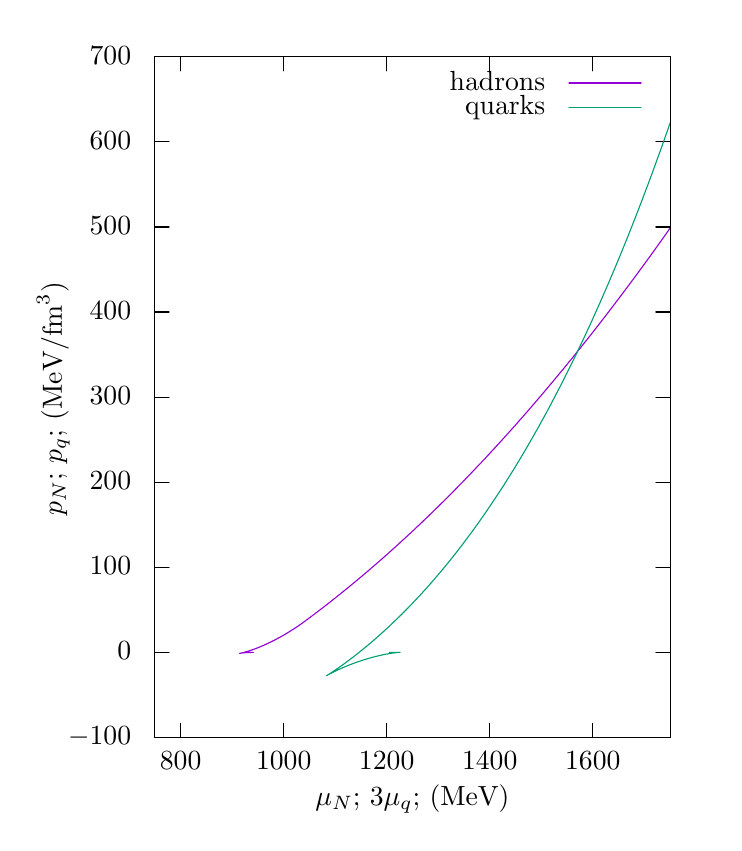
\begin{tikzpicture}[gnuplot]
%% generated with GNUPLOT 5.0p4 (Lua 5.2; terminal rev. 99, script rev. 100)
%% Thu Sep 29 16:33:15 2016
\path (0.000,0.000) rectangle (8.600,10.000);
\gpcolor{color=gp lt color border}
\gpsetlinetype{gp lt border}
\gpsetdashtype{gp dt solid}
\gpsetlinewidth{1.00}
\draw[gp path] (1.504,0.985)--(1.684,0.985);
\draw[gp path] (8.047,0.985)--(7.867,0.985);
\node[gp node right] at (1.320,0.985) {$-100$};
\draw[gp path] (1.504,2.066)--(1.684,2.066);
\draw[gp path] (8.047,2.066)--(7.867,2.066);
\node[gp node right] at (1.320,2.066) {$0$};
\draw[gp path] (1.504,3.147)--(1.684,3.147);
\draw[gp path] (8.047,3.147)--(7.867,3.147);
\node[gp node right] at (1.320,3.147) {$100$};
\draw[gp path] (1.504,4.227)--(1.684,4.227);
\draw[gp path] (8.047,4.227)--(7.867,4.227);
\node[gp node right] at (1.320,4.227) {$200$};
\draw[gp path] (1.504,5.308)--(1.684,5.308);
\draw[gp path] (8.047,5.308)--(7.867,5.308);
\node[gp node right] at (1.320,5.308) {$300$};
\draw[gp path] (1.504,6.389)--(1.684,6.389);
\draw[gp path] (8.047,6.389)--(7.867,6.389);
\node[gp node right] at (1.320,6.389) {$400$};
\draw[gp path] (1.504,7.469)--(1.684,7.469);
\draw[gp path] (8.047,7.469)--(7.867,7.469);
\node[gp node right] at (1.320,7.469) {$500$};
\draw[gp path] (1.504,8.550)--(1.684,8.550);
\draw[gp path] (8.047,8.550)--(7.867,8.550);
\node[gp node right] at (1.320,8.550) {$600$};
\draw[gp path] (1.504,9.631)--(1.684,9.631);
\draw[gp path] (8.047,9.631)--(7.867,9.631);
\node[gp node right] at (1.320,9.631) {$700$};
\draw[gp path] (1.831,0.985)--(1.831,1.165);
\draw[gp path] (1.831,9.631)--(1.831,9.451);
\node[gp node center] at (1.831,0.677) {$800$};
\draw[gp path] (3.140,0.985)--(3.140,1.165);
\draw[gp path] (3.140,9.631)--(3.140,9.451);
\node[gp node center] at (3.140,0.677) {$1000$};
\draw[gp path] (4.448,0.985)--(4.448,1.165);
\draw[gp path] (4.448,9.631)--(4.448,9.451);
\node[gp node center] at (4.448,0.677) {$1200$};
\draw[gp path] (5.757,0.985)--(5.757,1.165);
\draw[gp path] (5.757,9.631)--(5.757,9.451);
\node[gp node center] at (5.757,0.677) {$1400$};
\draw[gp path] (7.066,0.985)--(7.066,1.165);
\draw[gp path] (7.066,9.631)--(7.066,9.451);
\node[gp node center] at (7.066,0.677) {$1600$};
\draw[gp path] (1.504,9.631)--(1.504,0.985)--(8.047,0.985)--(8.047,9.631)--cycle;
\node[gp node center,rotate=-270] at (0.246,5.308) {$p_N$; $p_q$; ($\rm{MeV}/\rm{fm}^3$)};
\node[gp node center] at (4.775,0.215) {$\mu_N$; $3\mu_q$; (MeV)};
\node[gp node right] at (6.579,9.297) {hadrons};
\gpcolor{rgb color={0.580,0.000,0.827}}
\draw[gp path] (6.763,9.297)--(7.679,9.297);
\draw[gp path] (2.725,2.066)--(2.732,2.066)--(2.739,2.066)--(2.745,2.066)--(2.751,2.066)%
  --(2.757,2.066)--(2.725,2.066)--(2.731,2.066)--(2.737,2.066)--(2.743,2.066)--(2.748,2.066)%
  --(2.716,2.065)--(2.721,2.066)--(2.727,2.066)--(2.732,2.066)--(2.738,2.066)--(2.705,2.065)%
  --(2.711,2.065)--(2.716,2.065)--(2.722,2.066)--(2.727,2.066)--(2.733,2.066)--(2.700,2.065)%
  --(2.706,2.065)--(2.711,2.065)--(2.717,2.065)--(2.722,2.066)--(2.690,2.065)--(2.695,2.065)%
  --(2.700,2.065)--(2.706,2.065)--(2.711,2.065)--(2.679,2.064)--(2.684,2.064)--(2.690,2.065)%
  --(2.695,2.065)--(2.700,2.065)--(2.706,2.065)--(2.673,2.064)--(2.679,2.064)--(2.684,2.064)%
  --(2.690,2.065)--(2.695,2.065)--(2.663,2.063)--(2.668,2.063)--(2.674,2.064)--(2.679,2.064)%
  --(2.685,2.064)--(2.690,2.065)--(2.658,2.063)--(2.663,2.063)--(2.669,2.063)--(2.674,2.064)%
  --(2.680,2.064)--(2.648,2.062)--(2.653,2.063)--(2.659,2.063)--(2.664,2.063)--(2.670,2.064)%
  --(2.675,2.064)--(2.643,2.062)--(2.649,2.062)--(2.654,2.063)--(2.660,2.063)--(2.665,2.063)%
  --(2.634,2.061)--(2.639,2.061)--(2.645,2.062)--(2.650,2.062)--(2.656,2.063)--(2.661,2.063)%
  --(2.630,2.061)--(2.635,2.061)--(2.641,2.062)--(2.647,2.062)--(2.652,2.063)--(2.621,2.060)%
  --(2.626,2.060)--(2.632,2.061)--(2.638,2.061)--(2.643,2.062)--(2.649,2.062)--(2.617,2.059)%
  --(2.623,2.060)--(2.629,2.061)--(2.635,2.061)--(2.640,2.062)--(2.609,2.059)--(2.615,2.059)%
  --(2.620,2.060)--(2.626,2.060)--(2.632,2.061)--(2.638,2.061)--(2.606,2.058)--(2.612,2.059)%
  --(2.618,2.059)--(2.624,2.060)--(2.630,2.061)--(2.635,2.061)--(2.604,2.058)--(2.610,2.059)%
  --(2.616,2.059)--(2.622,2.060)--(2.628,2.061)--(2.597,2.057)--(2.602,2.058)--(2.608,2.058)%
  --(2.614,2.059)--(2.620,2.060)--(2.626,2.060)--(2.595,2.057)--(2.601,2.057)--(2.607,2.058)%
  --(2.613,2.059)--(2.619,2.060)--(2.588,2.056)--(2.594,2.056)--(2.600,2.057)--(2.606,2.058)%
  --(2.612,2.059)--(2.618,2.060)--(2.587,2.055)--(2.593,2.056)--(2.599,2.057)--(2.605,2.058)%
  --(2.611,2.059)--(2.618,2.060)--(2.587,2.055)--(2.593,2.056)--(2.599,2.057)--(2.605,2.058)%
  --(2.611,2.059)--(2.617,2.060)--(2.587,2.055)--(2.593,2.056)--(2.599,2.057)--(2.605,2.058)%
  --(2.612,2.059)--(2.581,2.054)--(2.588,2.055)--(2.594,2.056)--(2.600,2.057)--(2.606,2.058)%
  --(2.612,2.059)--(2.582,2.054)--(2.588,2.055)--(2.595,2.056)--(2.601,2.057)--(2.607,2.058)%
  --(2.613,2.059)--(2.583,2.054)--(2.590,2.055)--(2.596,2.057)--(2.602,2.058)--(2.608,2.059)%
  --(2.579,2.054)--(2.585,2.055)--(2.591,2.056)--(2.597,2.057)--(2.604,2.058)--(2.610,2.059)%
  --(2.580,2.054)--(2.587,2.055)--(2.593,2.056)--(2.600,2.057)--(2.606,2.058)--(2.612,2.060)%
  --(2.583,2.054)--(2.589,2.055)--(2.596,2.056)--(2.602,2.058)--(2.608,2.059)--(2.615,2.060)%
  --(2.585,2.054)--(2.592,2.056)--(2.598,2.057)--(2.605,2.058)--(2.611,2.059)--(2.618,2.061)%
  --(2.588,2.055)--(2.595,2.056)--(2.601,2.058)--(2.608,2.059)--(2.614,2.060)--(2.585,2.054)%
  --(2.592,2.056)--(2.598,2.057)--(2.605,2.058)--(2.611,2.060)--(2.618,2.061)--(2.589,2.055)%
  --(2.596,2.056)--(2.602,2.058)--(2.609,2.059)--(2.615,2.061)--(2.622,2.062)--(2.593,2.056)%
  --(2.600,2.057)--(2.606,2.059)--(2.613,2.060)--(2.620,2.062)--(2.626,2.063)--(2.598,2.057)%
  --(2.604,2.058)--(2.611,2.060)--(2.618,2.061)--(2.624,2.063)--(2.596,2.056)--(2.603,2.058)%
  --(2.609,2.059)--(2.616,2.061)--(2.623,2.062)--(2.629,2.064)--(2.601,2.057)--(2.608,2.059)%
  --(2.614,2.060)--(2.621,2.062)--(2.628,2.064)--(2.635,2.065)--(2.607,2.058)--(2.613,2.060)%
  --(2.620,2.062)--(2.627,2.063)--(2.634,2.065)--(2.640,2.067)--(2.612,2.060)--(2.619,2.062)%
  --(2.626,2.063)--(2.633,2.065)--(2.640,2.067)--(2.647,2.068)--(2.619,2.061)--(2.626,2.063)%
  --(2.632,2.065)--(2.639,2.067)--(2.646,2.068)--(2.619,2.061)--(2.625,2.063)--(2.632,2.065)%
  --(2.639,2.067)--(2.646,2.068)--(2.653,2.070)--(2.625,2.063)--(2.632,2.065)--(2.639,2.067)%
  --(2.646,2.069)--(2.653,2.070)--(2.660,2.072)--(2.633,2.065)--(2.640,2.067)--(2.647,2.069)%
  --(2.654,2.071)--(2.661,2.073)--(2.668,2.075)--(2.640,2.067)--(2.648,2.069)--(2.655,2.071)%
  --(2.662,2.073)--(2.669,2.075)--(2.676,2.077)--(2.649,2.069)--(2.656,2.071)--(2.663,2.073)%
  --(2.670,2.075)--(2.677,2.077)--(2.650,2.069)--(2.657,2.071)--(2.664,2.074)--(2.671,2.076)%
  --(2.678,2.078)--(2.685,2.080)--(2.659,2.072)--(2.666,2.074)--(2.673,2.076)--(2.680,2.078)%
  --(2.687,2.080)--(2.694,2.083)--(2.668,2.074)--(2.675,2.077)--(2.682,2.079)--(2.689,2.081)%
  --(2.696,2.083)--(2.703,2.086)--(2.677,2.077)--(2.684,2.080)--(2.691,2.082)--(2.699,2.084)%
  --(2.706,2.086)--(2.679,2.078)--(2.687,2.080)--(2.694,2.083)--(2.701,2.085)--(2.708,2.087)%
  --(2.716,2.090)--(2.689,2.081)--(2.697,2.084)--(2.704,2.086)--(2.711,2.088)--(2.719,2.091)%
  --(2.726,2.093)--(2.700,2.084)--(2.707,2.087)--(2.714,2.089)--(2.722,2.092)--(2.729,2.094)%
  --(2.736,2.097)--(2.710,2.088)--(2.718,2.090)--(2.725,2.093)--(2.732,2.095)--(2.740,2.098)%
  --(2.714,2.089)--(2.722,2.092)--(2.729,2.094)--(2.736,2.097)--(2.744,2.099)--(2.751,2.102)%
  --(2.725,2.093)--(2.733,2.096)--(2.740,2.098)--(2.748,2.101)--(2.755,2.103)--(2.762,2.106)%
  --(2.737,2.097)--(2.745,2.100)--(2.752,2.102)--(2.759,2.105)--(2.767,2.108)--(2.742,2.099)%
  --(2.749,2.101)--(2.757,2.104)--(2.764,2.107)--(2.771,2.109)--(2.779,2.112)--(2.754,2.103)%
  --(2.761,2.106)--(2.769,2.109)--(2.776,2.111)--(2.784,2.114)--(2.767,2.108)--(2.775,2.111)%
  --(2.782,2.113)--(2.773,2.110)--(2.781,2.113)--(2.788,2.116)--(2.780,2.113)--(2.787,2.116)%
  --(2.795,2.118)--(2.786,2.115)--(2.794,2.118)--(2.801,2.121)--(2.793,2.118)--(2.801,2.121)%
  --(2.792,2.117)--(2.800,2.120)--(2.807,2.123)--(2.799,2.120)--(2.806,2.123)--(2.814,2.126)%
  --(2.806,2.123)--(2.813,2.126)--(2.821,2.129)--(2.813,2.125)--(2.820,2.128)--(2.812,2.125)%
  --(2.820,2.128)--(2.827,2.131)--(2.819,2.128)--(2.827,2.131)--(2.834,2.134)--(2.826,2.131)%
  --(2.834,2.134)--(2.841,2.137)--(2.833,2.134)--(2.841,2.137)--(2.833,2.134)--(2.841,2.137)%
  --(2.848,2.140)--(2.840,2.137)--(2.848,2.140)--(2.856,2.143)--(2.848,2.140)--(2.855,2.143)%
  --(2.848,2.140)--(2.855,2.143)--(2.863,2.146)--(2.855,2.143)--(2.863,2.146)--(2.871,2.149)%
  --(2.863,2.146)--(2.870,2.149)--(2.863,2.146)--(2.870,2.149)--(2.878,2.153)--(2.871,2.149)%
  --(2.878,2.153)--(2.886,2.156)--(2.878,2.153)--(2.886,2.156)--(2.879,2.153)--(2.886,2.156)%
  --(2.894,2.160)--(2.887,2.156)--(2.894,2.160)--(2.902,2.163)--(2.895,2.160)--(2.902,2.163)%
  --(2.895,2.160)--(2.903,2.164)--(2.910,2.167)--(2.903,2.164)--(2.911,2.167)--(2.919,2.171)%
  --(2.911,2.168)--(2.919,2.171)--(2.912,2.168)--(2.920,2.171)--(2.927,2.175)--(2.920,2.172)%
  --(2.928,2.175)--(2.921,2.172)--(2.929,2.176)--(2.937,2.179)--(2.929,2.176)--(2.937,2.180)%
  --(2.945,2.183)--(2.938,2.180)--(2.946,2.184)--(2.939,2.180)--(2.947,2.184)--(2.955,2.188)%
  --(2.948,2.184)--(2.955,2.188)--(2.949,2.185)--(2.956,2.189)--(2.964,2.192)--(2.957,2.189)%
  --(2.965,2.193)--(2.959,2.190)--(2.966,2.193)--(2.974,2.197)--(2.968,2.194)--(2.975,2.198)%
  --(2.969,2.195)--(2.977,2.198)--(2.984,2.202)--(2.978,2.199)--(2.986,2.203)--(2.979,2.200)%
  --(2.987,2.204)--(2.995,2.208)--(2.988,2.204)--(2.996,2.208)--(2.990,2.205)--(2.998,2.209)%
  --(3.006,2.213)--(2.999,2.210)--(3.007,2.214)--(3.001,2.210)--(3.009,2.214)--(3.017,2.218)%
  --(3.010,2.215)--(3.018,2.219)--(3.012,2.216)--(3.020,2.220)--(3.014,2.217)--(3.022,2.221)%
  --(3.030,2.225)--(3.024,2.222)--(3.031,2.226)--(3.025,2.223)--(3.033,2.227)--(3.041,2.231)%
  --(3.035,2.228)--(3.043,2.232)--(3.037,2.229)--(3.045,2.233)--(3.039,2.230)--(3.047,2.234)%
  --(3.055,2.239)--(3.049,2.236)--(3.057,2.240)--(3.052,2.237)--(3.060,2.241)--(3.054,2.238)%
  --(3.062,2.242)--(3.070,2.246)--(3.064,2.243)--(3.072,2.248)--(3.066,2.245)--(3.074,2.249)%
  --(3.069,2.246)--(3.077,2.250)--(3.085,2.255)--(3.079,2.252)--(3.087,2.256)--(3.082,2.253)%
  --(3.090,2.257)--(3.084,2.254)--(3.092,2.259)--(3.100,2.263)--(3.095,2.260)--(3.103,2.265)%
  --(3.098,2.262)--(3.106,2.266)--(3.101,2.263)--(3.109,2.268)--(3.103,2.265)--(3.111,2.269)%
  --(3.106,2.267)--(3.114,2.271)--(3.122,2.275)--(3.117,2.273)--(3.125,2.277)--(3.120,2.274)%
  --(3.128,2.279)--(3.124,2.276)--(3.132,2.281)--(3.127,2.278)--(3.135,2.283)--(3.130,2.280)%
  --(3.138,2.284)--(3.133,2.282)--(3.141,2.286)--(3.149,2.291)--(3.145,2.288)--(3.153,2.293)%
  --(3.148,2.290)--(3.156,2.295)--(3.152,2.292)--(3.160,2.297)--(3.155,2.294)--(3.163,2.299)%
  --(3.159,2.297)--(3.167,2.301)--(3.163,2.299)--(3.171,2.303)--(3.166,2.301)--(3.174,2.306)%
  --(3.170,2.303)--(3.178,2.308)--(3.174,2.306)--(3.182,2.310)--(3.178,2.308)--(3.186,2.313)%
  --(3.182,2.310)--(3.190,2.315)--(3.186,2.313)--(3.194,2.318)--(3.190,2.315)--(3.198,2.320)%
  --(3.195,2.318)--(3.203,2.323)--(3.199,2.321)--(3.207,2.325)--(3.203,2.323)--(3.211,2.328)%
  --(3.208,2.326)--(3.216,2.331)--(3.212,2.329)--(3.220,2.334)--(3.217,2.332)--(3.225,2.337)%
  --(3.222,2.335)--(3.218,2.333)--(3.226,2.337)--(3.223,2.336)--(3.231,2.340)--(3.228,2.339)%
  --(3.236,2.344)--(3.233,2.342)--(3.241,2.347)--(3.238,2.345)--(3.246,2.350)--(3.243,2.348)%
  --(3.246,2.350)--(3.248,2.351)--(3.251,2.353)--(3.254,2.355)--(3.256,2.356)--(3.254,2.355)%
  --(3.257,2.357)--(3.259,2.358)--(3.262,2.360)--(3.265,2.362)--(3.268,2.364)--(3.266,2.362)%
  --(3.269,2.364)--(3.271,2.366)--(3.274,2.368)--(3.272,2.367)--(3.275,2.369)--(3.278,2.371)%
  --(3.281,2.373)--(3.284,2.375)--(3.283,2.373)--(3.286,2.375)--(3.289,2.378)--(3.287,2.376)%
  --(3.290,2.379)--(3.294,2.381)--(3.297,2.383)--(3.295,2.382)--(3.299,2.384)--(3.302,2.386)%
  --(3.301,2.385)--(3.304,2.388)--(3.308,2.390)--(3.306,2.389)--(3.310,2.392)--(3.309,2.391)%
  --(3.313,2.393)--(3.316,2.396)--(3.315,2.395)--(3.319,2.398)--(3.318,2.397)--(3.322,2.400)%
  --(3.321,2.399)--(3.325,2.402)--(3.329,2.404)--(3.332,2.407)--(3.336,2.410)--(3.337,2.410)%
  --(3.341,2.413)--(3.346,2.416)--(3.347,2.417)--(3.348,2.418)--(3.352,2.421)--(3.353,2.421)%
  --(3.354,2.422)--(3.355,2.423)--(3.356,2.424)--(3.358,2.425)--(3.359,2.426)--(3.361,2.427)%
  --(3.362,2.428)--(3.365,2.430)--(3.367,2.431)--(3.369,2.433)--(3.370,2.433)--(3.373,2.435)%
  --(3.374,2.436)--(3.375,2.437)--(3.377,2.438)--(3.378,2.439)--(3.380,2.441)--(3.381,2.441)%
  --(3.383,2.443)--(3.385,2.444)--(3.387,2.446)--(3.388,2.447)--(3.390,2.448)--(3.391,2.449)%
  --(3.393,2.450)--(3.394,2.451)--(3.396,2.452)--(3.397,2.453)--(3.398,2.454)--(3.400,2.455)%
  --(3.406,2.459)--(3.414,2.465)--(3.421,2.471)--(3.429,2.477)--(3.437,2.482)--(3.445,2.488)%
  --(3.452,2.494)--(3.460,2.500)--(3.468,2.505)--(3.476,2.511)--(3.483,2.517)--(3.491,2.523)%
  --(3.499,2.529)--(3.507,2.534)--(3.514,2.540)--(3.522,2.546)--(3.530,2.552)--(3.537,2.558)%
  --(3.545,2.564)--(3.553,2.570)--(3.561,2.575)--(3.568,2.581)--(3.576,2.587)--(3.584,2.593)%
  --(3.592,2.599)--(3.599,2.605)--(3.607,2.611)--(3.615,2.617)--(3.622,2.623)--(3.630,2.629)%
  --(3.638,2.634)--(3.646,2.640)--(3.653,2.646)--(3.661,2.652)--(3.669,2.658)--(3.676,2.664)%
  --(3.684,2.670)--(3.692,2.676)--(3.699,2.682)--(3.707,2.688)--(3.715,2.694)--(3.723,2.700)%
  --(3.730,2.706)--(3.738,2.712)--(3.746,2.718)--(3.753,2.725)--(3.761,2.731)--(3.769,2.737)%
  --(3.776,2.743)--(3.784,2.749)--(3.792,2.755)--(3.800,2.761)--(3.807,2.767)--(3.815,2.773)%
  --(3.823,2.779)--(3.830,2.786)--(3.838,2.792)--(3.846,2.798)--(3.853,2.804)--(3.861,2.810)%
  --(3.869,2.816)--(3.876,2.822)--(3.884,2.829)--(3.892,2.835)--(3.899,2.841)--(3.907,2.847)%
  --(3.915,2.854)--(3.922,2.860)--(3.930,2.866)--(3.938,2.872)--(3.945,2.878)--(3.953,2.885)%
  --(3.961,2.891)--(3.968,2.897)--(3.976,2.904)--(3.984,2.910)--(3.991,2.916)--(3.999,2.922)%
  --(4.007,2.929)--(4.014,2.935)--(4.022,2.941)--(4.030,2.948)--(4.037,2.954)--(4.045,2.960)%
  --(4.053,2.967)--(4.060,2.973)--(4.068,2.979)--(4.076,2.986)--(4.083,2.992)--(4.091,2.999)%
  --(4.099,3.005)--(4.106,3.011)--(4.114,3.018)--(4.122,3.024)--(4.129,3.031)--(4.137,3.037)%
  --(4.144,3.044)--(4.152,3.050)--(4.160,3.056)--(4.167,3.063)--(4.175,3.069)--(4.183,3.076)%
  --(4.190,3.082)--(4.198,3.089)--(4.206,3.095)--(4.213,3.102)--(4.221,3.108)--(4.228,3.115)%
  --(4.236,3.122)--(4.244,3.128)--(4.251,3.135)--(4.259,3.141)--(4.267,3.148)--(4.274,3.154)%
  --(4.282,3.161)--(4.289,3.167)--(4.297,3.174)--(4.305,3.181)--(4.312,3.187)--(4.320,3.194)%
  --(4.328,3.201)--(4.335,3.207)--(4.343,3.214)--(4.350,3.220)--(4.358,3.227)--(4.366,3.234)%
  --(4.373,3.240)--(4.381,3.247)--(4.389,3.254)--(4.396,3.261)--(4.404,3.267)--(4.411,3.274)%
  --(4.419,3.281)--(4.427,3.287)--(4.434,3.294)--(4.442,3.301)--(4.449,3.308)--(4.457,3.314)%
  --(4.465,3.321)--(4.472,3.328)--(4.480,3.335)--(4.487,3.342)--(4.495,3.348)--(4.503,3.355)%
  --(4.510,3.362)--(4.518,3.369)--(4.525,3.376)--(4.533,3.382)--(4.541,3.389)--(4.548,3.396)%
  --(4.556,3.403)--(4.563,3.410)--(4.571,3.417)--(4.579,3.424)--(4.586,3.430)--(4.594,3.437)%
  --(4.601,3.444)--(4.609,3.451)--(4.617,3.458)--(4.624,3.465)--(4.632,3.472)--(4.639,3.479)%
  --(4.647,3.486)--(4.654,3.493)--(4.662,3.500)--(4.670,3.507)--(4.677,3.514)--(4.685,3.521)%
  --(4.692,3.528)--(4.700,3.535)--(4.708,3.542)--(4.715,3.549)--(4.723,3.556)--(4.730,3.563)%
  --(4.738,3.570)--(4.745,3.577)--(4.753,3.584)--(4.761,3.591)--(4.768,3.598)--(4.776,3.605)%
  --(4.783,3.612)--(4.791,3.619)--(4.798,3.626)--(4.806,3.633)--(4.814,3.641)--(4.821,3.648)%
  --(4.829,3.655)--(4.836,3.662)--(4.844,3.669)--(4.851,3.676)--(4.859,3.683)--(4.866,3.691)%
  --(4.874,3.698)--(4.882,3.705)--(4.889,3.712)--(4.897,3.719)--(4.904,3.727)--(4.912,3.734)%
  --(4.919,3.741)--(4.927,3.748)--(4.934,3.755)--(4.942,3.763)--(4.950,3.770)--(4.957,3.777)%
  --(4.965,3.784)--(4.972,3.792)--(4.980,3.799)--(4.987,3.806)--(4.995,3.814)--(5.002,3.821)%
  --(5.010,3.828)--(5.017,3.835)--(5.025,3.843)--(5.033,3.850)--(5.040,3.857)--(5.048,3.865)%
  --(5.055,3.872)--(5.063,3.880)--(5.070,3.887)--(5.078,3.894)--(5.085,3.902)--(5.093,3.909)%
  --(5.100,3.916)--(5.108,3.924)--(5.116,3.931)--(5.123,3.939)--(5.131,3.946)--(5.138,3.954)%
  --(5.146,3.961)--(5.153,3.969)--(5.161,3.976)--(5.168,3.983)--(5.176,3.991)--(5.183,3.998)%
  --(5.191,4.006)--(5.198,4.013)--(5.206,4.021)--(5.213,4.028)--(5.221,4.036)--(5.228,4.043)%
  --(5.236,4.051)--(5.243,4.059)--(5.251,4.066)--(5.259,4.074)--(5.266,4.081)--(5.274,4.089)%
  --(5.281,4.096)--(5.289,4.104)--(5.296,4.112)--(5.304,4.119)--(5.311,4.127)--(5.319,4.134)%
  --(5.326,4.142)--(5.334,4.150)--(5.341,4.157)--(5.349,4.165)--(5.356,4.173)--(5.364,4.180)%
  --(5.371,4.188)--(5.379,4.196)--(5.386,4.203)--(5.394,4.211)--(5.401,4.219)--(5.409,4.226)%
  --(5.416,4.234)--(5.424,4.242)--(5.431,4.250)--(5.439,4.257)--(5.446,4.265)--(5.454,4.273)%
  --(5.461,4.281)--(5.469,4.288)--(5.476,4.296)--(5.484,4.304)--(5.491,4.312)--(5.499,4.320)%
  --(5.506,4.327)--(5.514,4.335)--(5.521,4.343)--(5.529,4.351)--(5.536,4.359)--(5.544,4.367)%
  --(5.551,4.374)--(5.559,4.382)--(5.566,4.390)--(5.574,4.398)--(5.581,4.406)--(5.589,4.414)%
  --(5.596,4.422)--(5.604,4.430)--(5.611,4.438)--(5.619,4.445)--(5.626,4.453)--(5.634,4.461)%
  --(5.641,4.469)--(5.649,4.477)--(5.656,4.485)--(5.664,4.493)--(5.671,4.501)--(5.679,4.509)%
  --(5.686,4.517)--(5.694,4.525)--(5.701,4.533)--(5.709,4.541)--(5.716,4.549)--(5.724,4.557)%
  --(5.731,4.565)--(5.738,4.573)--(5.746,4.581)--(5.753,4.589)--(5.761,4.597)--(5.768,4.606)%
  --(5.776,4.614)--(5.783,4.622)--(5.791,4.630)--(5.798,4.638)--(5.806,4.646)--(5.813,4.654)%
  --(5.821,4.662)--(5.828,4.670)--(5.836,4.679)--(5.843,4.687)--(5.851,4.695)--(5.858,4.703)%
  --(5.865,4.711)--(5.873,4.719)--(5.880,4.728)--(5.888,4.736)--(5.895,4.744)--(5.903,4.752)%
  --(5.910,4.760)--(5.918,4.769)--(5.925,4.777)--(5.933,4.785)--(5.940,4.793)--(5.948,4.802)%
  --(5.955,4.810)--(5.963,4.818)--(5.970,4.826)--(5.977,4.835)--(5.985,4.843)--(5.992,4.851)%
  --(6.000,4.860)--(6.007,4.868)--(6.015,4.876)--(6.022,4.885)--(6.030,4.893)--(6.037,4.901)%
  --(6.045,4.910)--(6.052,4.918)--(6.059,4.926)--(6.067,4.935)--(6.074,4.943)--(6.082,4.951)%
  --(6.089,4.960)--(6.097,4.968)--(6.104,4.977)--(6.112,4.985)--(6.119,4.994)--(6.126,5.002)%
  --(6.134,5.010)--(6.141,5.019)--(6.149,5.027)--(6.156,5.036)--(6.164,5.044)--(6.171,5.053)%
  --(6.179,5.061)--(6.186,5.070)--(6.193,5.078)--(6.201,5.087)--(6.208,5.095)--(6.216,5.104)%
  --(6.223,5.112)--(6.231,5.121)--(6.238,5.129)--(6.246,5.138)--(6.253,5.147)--(6.260,5.155)%
  --(6.268,5.164)--(6.275,5.172)--(6.283,5.181)--(6.290,5.189)--(6.298,5.198)--(6.305,5.207)%
  --(6.312,5.215)--(6.320,5.224)--(6.327,5.233)--(6.335,5.241)--(6.342,5.250)--(6.350,5.259)%
  --(6.357,5.267)--(6.364,5.276)--(6.372,5.285)--(6.379,5.293)--(6.387,5.302)--(6.394,5.311)%
  --(6.402,5.319)--(6.409,5.328)--(6.416,5.337)--(6.424,5.346)--(6.431,5.354)--(6.439,5.363)%
  --(6.446,5.372)--(6.454,5.381)--(6.461,5.389)--(6.468,5.398)--(6.476,5.407)--(6.483,5.416)%
  --(6.491,5.425)--(6.498,5.433)--(6.505,5.442)--(6.513,5.451)--(6.520,5.460)--(6.528,5.469)%
  --(6.535,5.478)--(6.543,5.486)--(6.550,5.495)--(6.557,5.504)--(6.565,5.513)--(6.572,5.522)%
  --(6.580,5.531)--(6.587,5.540)--(6.594,5.549)--(6.602,5.558)--(6.609,5.566)--(6.617,5.575)%
  --(6.624,5.584)--(6.631,5.593)--(6.639,5.602)--(6.646,5.611)--(6.654,5.620)--(6.661,5.629)%
  --(6.669,5.638)--(6.676,5.647)--(6.683,5.656)--(6.691,5.665)--(6.698,5.674)--(6.706,5.683)%
  --(6.713,5.692)--(6.720,5.701)--(6.728,5.710)--(6.735,5.719)--(6.743,5.728)--(6.750,5.737)%
  --(6.757,5.747)--(6.765,5.756)--(6.772,5.765)--(6.780,5.774)--(6.787,5.783)--(6.794,5.792)%
  --(6.802,5.801)--(6.809,5.810)--(6.817,5.819)--(6.824,5.829)--(6.831,5.838)--(6.839,5.847)%
  --(6.846,5.856)--(6.853,5.865)--(6.861,5.874)--(6.868,5.884)--(6.876,5.893)--(6.883,5.902)%
  --(6.890,5.911)--(6.898,5.920)--(6.905,5.930)--(6.913,5.939)--(6.920,5.948)--(6.927,5.957)%
  --(6.935,5.967)--(6.942,5.976)--(6.950,5.985)--(6.957,5.994)--(6.964,6.004)--(6.972,6.013)%
  --(6.979,6.022)--(6.986,6.032)--(6.994,6.041)--(7.001,6.050)--(7.009,6.060)--(7.016,6.069)%
  --(7.023,6.078)--(7.031,6.088)--(7.038,6.097)--(7.046,6.106)--(7.053,6.116)--(7.060,6.125)%
  --(7.068,6.134)--(7.075,6.144)--(7.082,6.153)--(7.090,6.163)--(7.097,6.172)--(7.105,6.182)%
  --(7.112,6.191)--(7.119,6.200)--(7.127,6.210)--(7.134,6.219)--(7.141,6.229)--(7.149,6.238)%
  --(7.156,6.248)--(7.164,6.257)--(7.171,6.267)--(7.178,6.276)--(7.186,6.286)--(7.193,6.295)%
  --(7.200,6.305)--(7.208,6.314)--(7.215,6.324)--(7.223,6.333)--(7.230,6.343)--(7.237,6.353)%
  --(7.245,6.362)--(7.252,6.372)--(7.259,6.381)--(7.267,6.391)--(7.274,6.400)--(7.281,6.410)%
  --(7.289,6.420)--(7.296,6.429)--(7.304,6.439)--(7.311,6.449)--(7.318,6.458)--(7.326,6.468)%
  --(7.333,6.478)--(7.340,6.487)--(7.348,6.497)--(7.355,6.507)--(7.362,6.516)--(7.370,6.526)%
  --(7.377,6.536)--(7.384,6.545)--(7.392,6.555)--(7.399,6.565)--(7.407,6.575)--(7.414,6.584)%
  --(7.421,6.594)--(7.429,6.604)--(7.436,6.614)--(7.443,6.623)--(7.451,6.633)--(7.458,6.643)%
  --(7.465,6.653)--(7.473,6.663)--(7.480,6.672)--(7.487,6.682)--(7.495,6.692)--(7.502,6.702)%
  --(7.510,6.712)--(7.517,6.722)--(7.524,6.731)--(7.532,6.741)--(7.539,6.751)--(7.546,6.761)%
  --(7.554,6.771)--(7.561,6.781)--(7.568,6.791)--(7.576,6.801)--(7.583,6.810)--(7.590,6.820)%
  --(7.598,6.830)--(7.605,6.840)--(7.612,6.850)--(7.620,6.860)--(7.627,6.870)--(7.634,6.880)%
  --(7.642,6.890)--(7.649,6.900)--(7.656,6.910)--(7.664,6.920)--(7.671,6.930)--(7.678,6.940)%
  --(7.686,6.950)--(7.693,6.960)--(7.700,6.970)--(7.708,6.980)--(7.715,6.990)--(7.723,7.000)%
  --(7.730,7.010)--(7.737,7.020)--(7.745,7.031)--(7.752,7.041)--(7.759,7.051)--(7.767,7.061)%
  --(7.774,7.071)--(7.781,7.081)--(7.789,7.091)--(7.796,7.101)--(7.803,7.111)--(7.811,7.122)%
  --(7.818,7.132)--(7.825,7.142)--(7.833,7.152)--(7.840,7.162)--(7.847,7.172)--(7.855,7.183)%
  --(7.862,7.193)--(7.869,7.203)--(7.877,7.213)--(7.884,7.224)--(7.891,7.234)--(7.898,7.244)%
  --(7.906,7.254)--(7.913,7.264)--(7.920,7.275)--(7.928,7.285)--(7.935,7.295)--(7.942,7.306)%
  --(7.950,7.316)--(7.957,7.326)--(7.964,7.336)--(7.972,7.347)--(7.979,7.357)--(7.986,7.367)%
  --(7.994,7.378)--(8.001,7.388)--(8.008,7.398)--(8.016,7.409)--(8.023,7.419)--(8.030,7.430)%
  --(8.038,7.440)--(8.045,7.450)--(8.047,7.453);
\gpcolor{color=gp lt color border}
\node[gp node right] at (6.579,8.989) {quarks};
\gpcolor{rgb color={0.000,0.620,0.451}}
\draw[gp path] (6.763,8.989)--(7.679,8.989);
\draw[gp path] (4.482,2.066)--(4.515,2.066)--(4.537,2.066)--(4.554,2.066)--(4.566,2.066)%
  --(4.577,2.066)--(4.585,2.067)--(4.593,2.067)--(4.598,2.067)--(4.603,2.067)--(4.607,2.067)%
  --(4.611,2.067)--(4.614,2.067)--(4.616,2.067)--(4.617,2.068)--(4.618,2.068)--(4.619,2.068)%
  --(4.618,2.068)--(4.617,2.067)--(4.616,2.067)--(4.614,2.067)--(4.612,2.067)--(4.610,2.067)%
  --(4.608,2.067)--(4.606,2.067)--(4.603,2.066)--(4.601,2.066)--(4.598,2.066)--(4.595,2.066)%
  --(4.592,2.065)--(4.588,2.065)--(4.585,2.065)--(4.581,2.064)--(4.577,2.064)--(4.573,2.063)%
  --(4.569,2.063)--(4.565,2.063)--(4.561,2.062)--(4.557,2.062)--(4.552,2.061)--(4.548,2.060)%
  --(4.543,2.060)--(4.539,2.059)--(4.534,2.059)--(4.529,2.058)--(4.524,2.057)--(4.519,2.057)%
  --(4.514,2.056)--(4.509,2.055)--(4.504,2.054)--(4.499,2.053)--(4.493,2.053)--(4.488,2.052)%
  --(4.483,2.051)--(4.477,2.050)--(4.472,2.049)--(4.466,2.048)--(4.460,2.047)--(4.455,2.046)%
  --(4.449,2.045)--(4.443,2.044)--(4.437,2.043)--(4.431,2.042)--(4.425,2.040)--(4.419,2.039)%
  --(4.413,2.038)--(4.408,2.037)--(4.402,2.036)--(4.395,2.034)--(4.389,2.033)--(4.383,2.032)%
  --(4.377,2.030)--(4.371,2.029)--(4.364,2.028)--(4.358,2.026)--(4.352,2.025)--(4.345,2.023)%
  --(4.339,2.022)--(4.332,2.020)--(4.326,2.019)--(4.319,2.017)--(4.313,2.015)--(4.306,2.014)%
  --(4.300,2.012)--(4.293,2.010)--(4.287,2.009)--(4.280,2.007)--(4.273,2.005)--(4.267,2.003)%
  --(4.260,2.002)--(4.253,2.000)--(4.247,1.998)--(4.240,1.996)--(4.233,1.994)--(4.227,1.992)%
  --(4.220,1.990)--(4.213,1.988)--(4.206,1.986)--(4.200,1.984)--(4.193,1.982)--(4.186,1.980)%
  --(4.179,1.978)--(4.172,1.976)--(4.166,1.974)--(4.159,1.972)--(4.152,1.970)--(4.145,1.967)%
  --(4.138,1.965)--(4.131,1.963)--(4.125,1.961)--(4.118,1.958)--(4.111,1.956)--(4.104,1.954)%
  --(4.097,1.951)--(4.090,1.949)--(4.083,1.947)--(4.077,1.944)--(4.070,1.942)--(4.063,1.940)%
  --(4.056,1.937)--(4.049,1.935)--(4.043,1.932)--(4.036,1.930)--(4.029,1.927)--(4.022,1.925)%
  --(4.016,1.922)--(4.009,1.920)--(4.002,1.917)--(3.995,1.914)--(3.989,1.912)--(3.982,1.909)%
  --(3.975,1.907)--(3.969,1.904)--(3.962,1.901)--(3.956,1.899)--(3.949,1.896)--(3.943,1.893)%
  --(3.936,1.891)--(3.930,1.888)--(3.923,1.885)--(3.917,1.882)--(3.910,1.880)--(3.904,1.877)%
  --(3.898,1.874)--(3.891,1.872)--(3.885,1.869)--(3.879,1.866)--(3.873,1.863)--(3.867,1.861)%
  --(3.861,1.858)--(3.855,1.855)--(3.849,1.853)--(3.843,1.850)--(3.837,1.847)--(3.831,1.845)%
  --(3.825,1.842)--(3.820,1.839)--(3.814,1.837)--(3.808,1.834)--(3.803,1.831)--(3.798,1.829)%
  --(3.792,1.826)--(3.787,1.824)--(3.782,1.821)--(3.777,1.819)--(3.772,1.816)--(3.767,1.814)%
  --(3.762,1.811)--(3.757,1.809)--(3.753,1.807)--(3.748,1.804)--(3.744,1.802)--(3.740,1.800)%
  --(3.736,1.798)--(3.732,1.796)--(3.728,1.794)--(3.724,1.792)--(3.720,1.790)--(3.717,1.788)%
  --(3.714,1.786)--(3.710,1.785)--(3.707,1.783)--(3.705,1.781)--(3.702,1.780)--(3.699,1.779)%
  --(3.697,1.777)--(3.695,1.776)--(3.693,1.775)--(3.691,1.774)--(3.690,1.773)--(3.688,1.772)%
  --(3.687,1.772)--(3.686,1.771)--(3.685,1.771)--(3.685,1.770)--(3.684,1.770)--(3.685,1.770)%
  --(3.685,1.771)--(3.686,1.771)--(3.687,1.772)--(3.689,1.773)--(3.690,1.773)--(3.692,1.775)%
  --(3.694,1.776)--(3.696,1.777)--(3.698,1.779)--(3.701,1.780)--(3.704,1.782)--(3.707,1.784)%
  --(3.710,1.786)--(3.714,1.788)--(3.718,1.791)--(3.722,1.793)--(3.726,1.796)--(3.730,1.799)%
  --(3.735,1.802)--(3.739,1.805)--(3.744,1.808)--(3.749,1.811)--(3.755,1.815)--(3.760,1.818)%
  --(3.766,1.822)--(3.771,1.826)--(3.777,1.830)--(3.783,1.834)--(3.789,1.838)--(3.796,1.842)%
  --(3.802,1.847)--(3.809,1.851)--(3.815,1.856)--(3.822,1.860)--(3.829,1.865)--(3.836,1.870)%
  --(3.843,1.875)--(3.850,1.880)--(3.857,1.885)--(3.864,1.890)--(3.872,1.895)--(3.879,1.901)%
  --(3.887,1.906)--(3.894,1.911)--(3.902,1.917)--(3.909,1.922)--(3.917,1.928)--(3.925,1.934)%
  --(3.933,1.939)--(3.940,1.945)--(3.948,1.951)--(3.956,1.957)--(3.964,1.963)--(3.972,1.969)%
  --(3.980,1.975)--(3.988,1.981)--(3.996,1.987)--(4.004,1.993)--(4.013,2.000)--(4.021,2.006)%
  --(4.029,2.012)--(4.037,2.018)--(4.045,2.025)--(4.053,2.031)--(4.062,2.038)--(4.070,2.044)%
  --(4.078,2.051)--(4.086,2.057)--(4.095,2.064)--(4.103,2.070)--(4.111,2.077)--(4.119,2.084)%
  --(4.128,2.090)--(4.136,2.097)--(4.144,2.104)--(4.153,2.110)--(4.161,2.117)--(4.169,2.124)%
  --(4.177,2.131)--(4.186,2.138)--(4.194,2.145)--(4.202,2.151)--(4.211,2.158)--(4.219,2.165)%
  --(4.227,2.172)--(4.235,2.179)--(4.244,2.186)--(4.252,2.193)--(4.260,2.200)--(4.268,2.207)%
  --(4.277,2.214)--(4.285,2.221)--(4.293,2.229)--(4.301,2.236)--(4.309,2.243)--(4.318,2.250)%
  --(4.326,2.257)--(4.334,2.264)--(4.342,2.272)--(4.350,2.279)--(4.358,2.286)--(4.367,2.293)%
  --(4.375,2.301)--(4.383,2.308)--(4.391,2.315)--(4.399,2.323)--(4.407,2.330)--(4.415,2.337)%
  --(4.423,2.345)--(4.431,2.352)--(4.439,2.359)--(4.448,2.367)--(4.456,2.374)--(4.464,2.382)%
  --(4.472,2.389)--(4.480,2.396)--(4.488,2.404)--(4.496,2.411)--(4.503,2.419)--(4.511,2.426)%
  --(4.519,2.434)--(4.527,2.442)--(4.535,2.449)--(4.543,2.457)--(4.551,2.464)--(4.559,2.472)%
  --(4.567,2.479)--(4.575,2.487)--(4.582,2.495)--(4.590,2.502)--(4.598,2.510)--(4.606,2.517)%
  --(4.614,2.525)--(4.621,2.533)--(4.629,2.540)--(4.637,2.548)--(4.645,2.556)--(4.652,2.564)%
  --(4.660,2.571)--(4.668,2.579)--(4.676,2.587)--(4.683,2.595)--(4.691,2.602)--(4.699,2.610)%
  --(4.706,2.618)--(4.714,2.626)--(4.722,2.633)--(4.729,2.641)--(4.737,2.649)--(4.744,2.657)%
  --(4.752,2.665)--(4.759,2.673)--(4.767,2.680)--(4.775,2.688)--(4.782,2.696)--(4.790,2.704)%
  --(4.797,2.712)--(4.805,2.720)--(4.812,2.728)--(4.819,2.736)--(4.827,2.744)--(4.834,2.752)%
  --(4.842,2.760)--(4.849,2.768)--(4.857,2.776)--(4.864,2.783)--(4.871,2.791)--(4.879,2.799)%
  --(4.886,2.807)--(4.893,2.816)--(4.901,2.824)--(4.908,2.832)--(4.915,2.840)--(4.923,2.848)%
  --(4.930,2.856)--(4.937,2.864)--(4.945,2.872)--(4.952,2.880)--(4.959,2.888)--(4.966,2.896)%
  --(4.973,2.904)--(4.981,2.912)--(4.988,2.920)--(4.995,2.929)--(5.002,2.937)--(5.009,2.945)%
  --(5.017,2.953)--(5.024,2.961)--(5.031,2.969)--(5.038,2.978)--(5.045,2.986)--(5.052,2.994)%
  --(5.059,3.002)--(5.066,3.010)--(5.073,3.019)--(5.080,3.027)--(5.087,3.035)--(5.094,3.043)%
  --(5.101,3.052)--(5.108,3.060)--(5.115,3.068)--(5.122,3.076)--(5.129,3.085)--(5.136,3.093)%
  --(5.143,3.101)--(5.150,3.110)--(5.157,3.118)--(5.164,3.126)--(5.171,3.135)--(5.178,3.143)%
  --(5.185,3.151)--(5.192,3.160)--(5.198,3.168)--(5.205,3.176)--(5.212,3.185)--(5.219,3.193)%
  --(5.226,3.201)--(5.233,3.210)--(5.239,3.218)--(5.246,3.227)--(5.253,3.235)--(5.260,3.244)%
  --(5.267,3.252)--(5.273,3.260)--(5.280,3.269)--(5.287,3.277)--(5.294,3.286)--(5.300,3.294)%
  --(5.307,3.303)--(5.314,3.311)--(5.320,3.320)--(5.327,3.328)--(5.334,3.337)--(5.340,3.345)%
  --(5.347,3.354)--(5.354,3.362)--(5.360,3.371)--(5.367,3.379)--(5.373,3.388)--(5.380,3.396)%
  --(5.387,3.405)--(5.393,3.414)--(5.400,3.422)--(5.406,3.431)--(5.413,3.439)--(5.419,3.448)%
  --(5.426,3.457)--(5.432,3.465)--(5.439,3.474)--(5.445,3.482)--(5.452,3.491)--(5.458,3.500)%
  --(5.465,3.508)--(5.471,3.517)--(5.478,3.526)--(5.484,3.534)--(5.491,3.543)--(5.497,3.552)%
  --(5.504,3.560)--(5.510,3.569)--(5.516,3.578)--(5.523,3.586)--(5.529,3.595)--(5.535,3.604)%
  --(5.542,3.613)--(5.548,3.621)--(5.555,3.630)--(5.561,3.639)--(5.567,3.648)--(5.574,3.656)%
  --(5.580,3.665)--(5.586,3.674)--(5.592,3.683)--(5.599,3.691)--(5.605,3.700)--(5.611,3.709)%
  --(5.618,3.718)--(5.624,3.727)--(5.630,3.735)--(5.636,3.744)--(5.642,3.753)--(5.649,3.762)%
  --(5.655,3.771)--(5.661,3.780)--(5.667,3.788)--(5.673,3.797)--(5.680,3.806)--(5.686,3.815)%
  --(5.692,3.824)--(5.698,3.833)--(5.704,3.842)--(5.710,3.851)--(5.717,3.859)--(5.723,3.868)%
  --(5.729,3.877)--(5.735,3.886)--(5.741,3.895)--(5.747,3.904)--(5.753,3.913)--(5.759,3.922)%
  --(5.765,3.931)--(5.771,3.940)--(5.777,3.949)--(5.783,3.958)--(5.789,3.967)--(5.795,3.976)%
  --(5.801,3.985)--(5.807,3.994)--(5.813,4.003)--(5.819,4.012)--(5.825,4.021)--(5.831,4.030)%
  --(5.837,4.039)--(5.843,4.048)--(5.849,4.057)--(5.855,4.066)--(5.861,4.075)--(5.867,4.084)%
  --(5.873,4.093)--(5.879,4.102)--(5.885,4.111)--(5.891,4.120)--(5.897,4.129)--(5.903,4.139)%
  --(5.908,4.148)--(5.914,4.157)--(5.920,4.166)--(5.926,4.175)--(5.932,4.184)--(5.938,4.193)%
  --(5.944,4.202)--(5.949,4.212)--(5.955,4.221)--(5.961,4.230)--(5.967,4.239)--(5.973,4.248)%
  --(5.978,4.257)--(5.984,4.266)--(5.990,4.276)--(5.996,4.285)--(6.002,4.294)--(6.007,4.303)%
  --(6.013,4.312)--(6.019,4.322)--(6.025,4.331)--(6.030,4.340)--(6.036,4.349)--(6.042,4.359)%
  --(6.047,4.368)--(6.053,4.377)--(6.059,4.386)--(6.065,4.396)--(6.070,4.405)--(6.076,4.414)%
  --(6.082,4.423)--(6.087,4.433)--(6.093,4.442)--(6.099,4.451)--(6.104,4.461)--(6.110,4.470)%
  --(6.115,4.479)--(6.121,4.488)--(6.127,4.498)--(6.132,4.507)--(6.138,4.516)--(6.144,4.526)%
  --(6.149,4.535)--(6.155,4.544)--(6.160,4.554)--(6.166,4.563)--(6.171,4.573)--(6.177,4.582)%
  --(6.183,4.591)--(6.188,4.601)--(6.194,4.610)--(6.199,4.619)--(6.205,4.629)--(6.210,4.638)%
  --(6.216,4.648)--(6.221,4.657)--(6.227,4.666)--(6.232,4.676)--(6.238,4.685)--(6.243,4.695)%
  --(6.249,4.704)--(6.254,4.714)--(6.260,4.723)--(6.265,4.733)--(6.270,4.742)--(6.276,4.751)%
  --(6.281,4.761)--(6.287,4.770)--(6.292,4.780)--(6.298,4.789)--(6.303,4.799)--(6.308,4.808)%
  --(6.314,4.818)--(6.319,4.827)--(6.325,4.837)--(6.330,4.846)--(6.335,4.856)--(6.341,4.866)%
  --(6.346,4.875)--(6.352,4.885)--(6.357,4.894)--(6.362,4.904)--(6.368,4.913)--(6.373,4.923)%
  --(6.378,4.932)--(6.384,4.942)--(6.389,4.952)--(6.394,4.961)--(6.400,4.971)--(6.405,4.980)%
  --(6.410,4.990)--(6.415,5.000)--(6.421,5.009)--(6.426,5.019)--(6.431,5.028)--(6.437,5.038)%
  --(6.442,5.048)--(6.447,5.057)--(6.452,5.067)--(6.458,5.077)--(6.463,5.086)--(6.468,5.096)%
  --(6.473,5.106)--(6.479,5.115)--(6.484,5.125)--(6.489,5.135)--(6.494,5.144)--(6.499,5.154)%
  --(6.505,5.164)--(6.510,5.173)--(6.515,5.183)--(6.520,5.193)--(6.525,5.203)--(6.531,5.212)%
  --(6.536,5.222)--(6.541,5.232)--(6.546,5.241)--(6.551,5.251)--(6.556,5.261)--(6.561,5.271)%
  --(6.567,5.280)--(6.572,5.290)--(6.577,5.300)--(6.582,5.310)--(6.587,5.320)--(6.592,5.329)%
  --(6.597,5.339)--(6.602,5.349)--(6.607,5.359)--(6.613,5.369)--(6.618,5.378)--(6.623,5.388)%
  --(6.628,5.398)--(6.633,5.408)--(6.638,5.418)--(6.643,5.427)--(6.648,5.437)--(6.653,5.447)%
  --(6.658,5.457)--(6.663,5.467)--(6.668,5.477)--(6.673,5.487)--(6.678,5.496)--(6.683,5.506)%
  --(6.688,5.516)--(6.693,5.526)--(6.698,5.536)--(6.703,5.546)--(6.708,5.556)--(6.713,5.566)%
  --(6.718,5.576)--(6.723,5.586)--(6.728,5.595)--(6.733,5.605)--(6.738,5.615)--(6.743,5.625)%
  --(6.748,5.635)--(6.753,5.645)--(6.758,5.655)--(6.763,5.665)--(6.768,5.675)--(6.773,5.685)%
  --(6.778,5.695)--(6.783,5.705)--(6.788,5.715)--(6.792,5.725)--(6.797,5.735)--(6.802,5.745)%
  --(6.807,5.755)--(6.812,5.765)--(6.817,5.775)--(6.822,5.785)--(6.827,5.795)--(6.832,5.805)%
  --(6.836,5.815)--(6.841,5.825)--(6.846,5.835)--(6.851,5.845)--(6.856,5.855)--(6.861,5.865)%
  --(6.866,5.875)--(6.870,5.885)--(6.875,5.895)--(6.880,5.905)--(6.885,5.915)--(6.890,5.925)%
  --(6.894,5.936)--(6.899,5.946)--(6.904,5.956)--(6.909,5.966)--(6.914,5.976)--(6.918,5.986)%
  --(6.923,5.996)--(6.928,6.006)--(6.933,6.016)--(6.938,6.027)--(6.942,6.037)--(6.947,6.047)%
  --(6.952,6.057)--(6.957,6.067)--(6.961,6.077)--(6.966,6.087)--(6.971,6.098)--(6.976,6.108)%
  --(6.980,6.118)--(6.985,6.128)--(6.990,6.138)--(6.995,6.148)--(6.999,6.159)--(7.004,6.169)%
  --(7.009,6.179)--(7.013,6.189)--(7.018,6.199)--(7.023,6.210)--(7.027,6.220)--(7.032,6.230)%
  --(7.037,6.240)--(7.042,6.251)--(7.046,6.261)--(7.051,6.271)--(7.056,6.281)--(7.060,6.291)%
  --(7.065,6.302)--(7.070,6.312)--(7.074,6.322)--(7.079,6.333)--(7.083,6.343)--(7.088,6.353)%
  --(7.093,6.363)--(7.097,6.374)--(7.102,6.384)--(7.107,6.394)--(7.111,6.405)--(7.116,6.415)%
  --(7.120,6.425)--(7.125,6.435)--(7.130,6.446)--(7.134,6.456)--(7.139,6.466)--(7.143,6.477)%
  --(7.148,6.487)--(7.153,6.497)--(7.157,6.508)--(7.162,6.518)--(7.166,6.528)--(7.171,6.539)%
  --(7.175,6.549)--(7.180,6.560)--(7.185,6.570)--(7.189,6.580)--(7.194,6.591)--(7.198,6.601)%
  --(7.203,6.611)--(7.207,6.622)--(7.212,6.632)--(7.216,6.643)--(7.221,6.653)--(7.225,6.663)%
  --(7.230,6.674)--(7.234,6.684)--(7.239,6.695)--(7.243,6.705)--(7.248,6.716)--(7.252,6.726)%
  --(7.257,6.736)--(7.261,6.747)--(7.266,6.757)--(7.270,6.768)--(7.275,6.778)--(7.279,6.789)%
  --(7.284,6.799)--(7.288,6.810)--(7.293,6.820)--(7.297,6.831)--(7.302,6.841)--(7.306,6.852)%
  --(7.311,6.862)--(7.315,6.873)--(7.319,6.883)--(7.324,6.894)--(7.328,6.904)--(7.333,6.915)%
  --(7.337,6.925)--(7.342,6.936)--(7.346,6.946)--(7.350,6.957)--(7.355,6.967)--(7.359,6.978)%
  --(7.364,6.988)--(7.368,6.999)--(7.372,7.009)--(7.377,7.020)--(7.381,7.031)--(7.386,7.041)%
  --(7.390,7.052)--(7.394,7.062)--(7.399,7.073)--(7.403,7.083)--(7.408,7.094)--(7.412,7.105)%
  --(7.416,7.115)--(7.421,7.126)--(7.425,7.136)--(7.429,7.147)--(7.434,7.158)--(7.438,7.168)%
  --(7.442,7.179)--(7.447,7.190)--(7.451,7.200)--(7.455,7.211)--(7.460,7.222)--(7.464,7.232)%
  --(7.468,7.243)--(7.473,7.253)--(7.477,7.264)--(7.481,7.275)--(7.486,7.285)--(7.490,7.296)%
  --(7.494,7.307)--(7.498,7.317)--(7.503,7.328)--(7.507,7.339)--(7.511,7.350)--(7.516,7.360)%
  --(7.520,7.371)--(7.524,7.382)--(7.528,7.392)--(7.533,7.403)--(7.537,7.414)--(7.541,7.425)%
  --(7.546,7.435)--(7.550,7.446)--(7.554,7.457)--(7.558,7.467)--(7.563,7.478)--(7.567,7.489)%
  --(7.571,7.500)--(7.575,7.510)--(7.579,7.521)--(7.584,7.532)--(7.588,7.543)--(7.592,7.554)%
  --(7.596,7.564)--(7.601,7.575)--(7.605,7.586)--(7.609,7.597)--(7.613,7.607)--(7.617,7.618)%
  --(7.622,7.629)--(7.626,7.640)--(7.630,7.651)--(7.634,7.661)--(7.638,7.672)--(7.643,7.683)%
  --(7.647,7.694)--(7.651,7.705)--(7.655,7.716)--(7.659,7.726)--(7.663,7.737)--(7.668,7.748)%
  --(7.672,7.759)--(7.676,7.770)--(7.680,7.781)--(7.684,7.792)--(7.688,7.802)--(7.693,7.813)%
  --(7.697,7.824)--(7.701,7.835)--(7.705,7.846)--(7.709,7.857)--(7.713,7.868)--(7.717,7.879)%
  --(7.722,7.890)--(7.726,7.900)--(7.730,7.911)--(7.734,7.922)--(7.738,7.933)--(7.742,7.944)%
  --(7.746,7.955)--(7.750,7.966)--(7.754,7.977)--(7.759,7.988)--(7.763,7.999)--(7.767,8.010)%
  --(7.771,8.021)--(7.775,8.032)--(7.779,8.043)--(7.783,8.054)--(7.787,8.064)--(7.791,8.075)%
  --(7.795,8.086)--(7.799,8.097)--(7.803,8.108)--(7.808,8.119)--(7.812,8.130)--(7.816,8.141)%
  --(7.820,8.152)--(7.824,8.163)--(7.828,8.174)--(7.832,8.185)--(7.836,8.196)--(7.840,8.207)%
  --(7.844,8.218)--(7.848,8.229)--(7.852,8.240)--(7.856,8.251)--(7.860,8.263)--(7.864,8.274)%
  --(7.868,8.285)--(7.872,8.296)--(7.876,8.307)--(7.880,8.318)--(7.884,8.329)--(7.888,8.340)%
  --(7.892,8.351)--(7.896,8.362)--(7.900,8.373)--(7.904,8.384)--(7.908,8.395)--(7.912,8.406)%
  --(7.916,8.417)--(7.920,8.429)--(7.924,8.440)--(7.928,8.451)--(7.932,8.462)--(7.936,8.473)%
  --(7.940,8.484)--(7.944,8.495)--(7.948,8.506)--(7.952,8.517)--(7.956,8.529)--(7.960,8.540)%
  --(7.964,8.551)--(7.968,8.562)--(7.972,8.573)--(7.976,8.584)--(7.980,8.595)--(7.983,8.607)%
  --(7.987,8.618)--(7.991,8.629)--(7.995,8.640)--(7.999,8.651)--(8.003,8.662)--(8.007,8.674)%
  --(8.011,8.685)--(8.015,8.696)--(8.019,8.707)--(8.023,8.718)--(8.027,8.730)--(8.031,8.741)%
  --(8.034,8.752)--(8.038,8.763)--(8.042,8.774)--(8.046,8.786)--(8.047,8.788);
\gpcolor{color=gp lt color border}
\draw[gp path] (1.504,9.631)--(1.504,0.985)--(8.047,0.985)--(8.047,9.631)--cycle;
%% coordinates of the plot area
\gpdefrectangularnode{gp plot 1}{\pgfpoint{1.504cm}{0.985cm}}{\pgfpoint{8.047cm}{9.631cm}}
\end{tikzpicture}
%% gnuplot variables

	\caption{BuballaR\_2-eNJL2OmegaRho1}
\end{figure}
\begin{figure}
	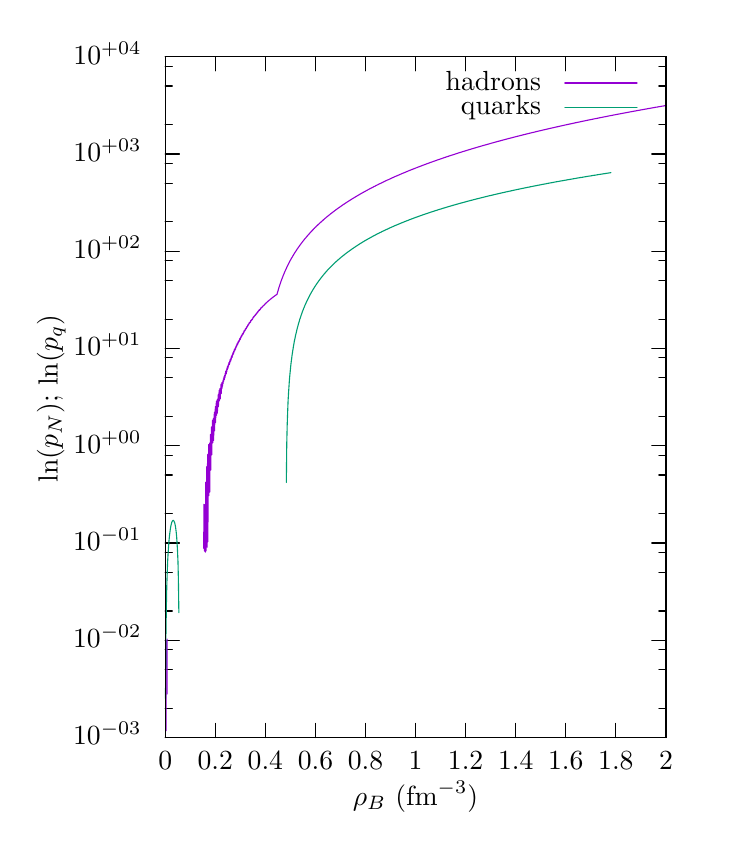
\begin{tikzpicture}[gnuplot]
%% generated with GNUPLOT 5.0p4 (Lua 5.2; terminal rev. 99, script rev. 100)
%% Thu Sep 29 16:33:15 2016
\path (0.000,0.000) rectangle (8.600,10.000);
\gpcolor{color=gp lt color border}
\gpsetlinetype{gp lt border}
\gpsetdashtype{gp dt solid}
\gpsetlinewidth{1.00}
\draw[gp path] (1.688,0.985)--(1.868,0.985);
\draw[gp path] (8.047,0.985)--(7.867,0.985);
\node[gp node right] at (1.504,0.985) {$10^{-03}$};
\draw[gp path] (1.688,1.357)--(1.778,1.357);
\draw[gp path] (8.047,1.357)--(7.957,1.357);
\draw[gp path] (1.688,1.848)--(1.778,1.848);
\draw[gp path] (8.047,1.848)--(7.957,1.848);
\draw[gp path] (1.688,2.100)--(1.778,2.100);
\draw[gp path] (8.047,2.100)--(7.957,2.100);
\draw[gp path] (1.688,2.220)--(1.868,2.220);
\draw[gp path] (8.047,2.220)--(7.867,2.220);
\node[gp node right] at (1.504,2.220) {$10^{-02}$};
\draw[gp path] (1.688,2.592)--(1.778,2.592);
\draw[gp path] (8.047,2.592)--(7.957,2.592);
\draw[gp path] (1.688,3.083)--(1.778,3.083);
\draw[gp path] (8.047,3.083)--(7.957,3.083);
\draw[gp path] (1.688,3.336)--(1.778,3.336);
\draw[gp path] (8.047,3.336)--(7.957,3.336);
\draw[gp path] (1.688,3.455)--(1.868,3.455);
\draw[gp path] (8.047,3.455)--(7.867,3.455);
\node[gp node right] at (1.504,3.455) {$10^{-01}$};
\draw[gp path] (1.688,3.827)--(1.778,3.827);
\draw[gp path] (8.047,3.827)--(7.957,3.827);
\draw[gp path] (1.688,4.319)--(1.778,4.319);
\draw[gp path] (8.047,4.319)--(7.957,4.319);
\draw[gp path] (1.688,4.571)--(1.778,4.571);
\draw[gp path] (8.047,4.571)--(7.957,4.571);
\draw[gp path] (1.688,4.690)--(1.868,4.690);
\draw[gp path] (8.047,4.690)--(7.867,4.690);
\node[gp node right] at (1.504,4.690) {$10^{+00}$};
\draw[gp path] (1.688,5.062)--(1.778,5.062);
\draw[gp path] (8.047,5.062)--(7.957,5.062);
\draw[gp path] (1.688,5.554)--(1.778,5.554);
\draw[gp path] (8.047,5.554)--(7.957,5.554);
\draw[gp path] (1.688,5.806)--(1.778,5.806);
\draw[gp path] (8.047,5.806)--(7.957,5.806);
\draw[gp path] (1.688,5.926)--(1.868,5.926);
\draw[gp path] (8.047,5.926)--(7.867,5.926);
\node[gp node right] at (1.504,5.926) {$10^{+01}$};
\draw[gp path] (1.688,6.297)--(1.778,6.297);
\draw[gp path] (8.047,6.297)--(7.957,6.297);
\draw[gp path] (1.688,6.789)--(1.778,6.789);
\draw[gp path] (8.047,6.789)--(7.957,6.789);
\draw[gp path] (1.688,7.041)--(1.778,7.041);
\draw[gp path] (8.047,7.041)--(7.957,7.041);
\draw[gp path] (1.688,7.161)--(1.868,7.161);
\draw[gp path] (8.047,7.161)--(7.867,7.161);
\node[gp node right] at (1.504,7.161) {$10^{+02}$};
\draw[gp path] (1.688,7.533)--(1.778,7.533);
\draw[gp path] (8.047,7.533)--(7.957,7.533);
\draw[gp path] (1.688,8.024)--(1.778,8.024);
\draw[gp path] (8.047,8.024)--(7.957,8.024);
\draw[gp path] (1.688,8.276)--(1.778,8.276);
\draw[gp path] (8.047,8.276)--(7.957,8.276);
\draw[gp path] (1.688,8.396)--(1.868,8.396);
\draw[gp path] (8.047,8.396)--(7.867,8.396);
\node[gp node right] at (1.504,8.396) {$10^{+03}$};
\draw[gp path] (1.688,8.768)--(1.778,8.768);
\draw[gp path] (8.047,8.768)--(7.957,8.768);
\draw[gp path] (1.688,9.259)--(1.778,9.259);
\draw[gp path] (8.047,9.259)--(7.957,9.259);
\draw[gp path] (1.688,9.511)--(1.778,9.511);
\draw[gp path] (8.047,9.511)--(7.957,9.511);
\draw[gp path] (1.688,9.631)--(1.868,9.631);
\draw[gp path] (8.047,9.631)--(7.867,9.631);
\node[gp node right] at (1.504,9.631) {$10^{+04}$};
\draw[gp path] (1.688,0.985)--(1.688,1.165);
\draw[gp path] (1.688,9.631)--(1.688,9.451);
\node[gp node center] at (1.688,0.677) {$0$};
\draw[gp path] (2.324,0.985)--(2.324,1.165);
\draw[gp path] (2.324,9.631)--(2.324,9.451);
\node[gp node center] at (2.324,0.677) {$0.2$};
\draw[gp path] (2.960,0.985)--(2.960,1.165);
\draw[gp path] (2.960,9.631)--(2.960,9.451);
\node[gp node center] at (2.960,0.677) {$0.4$};
\draw[gp path] (3.596,0.985)--(3.596,1.165);
\draw[gp path] (3.596,9.631)--(3.596,9.451);
\node[gp node center] at (3.596,0.677) {$0.6$};
\draw[gp path] (4.232,0.985)--(4.232,1.165);
\draw[gp path] (4.232,9.631)--(4.232,9.451);
\node[gp node center] at (4.232,0.677) {$0.8$};
\draw[gp path] (4.868,0.985)--(4.868,1.165);
\draw[gp path] (4.868,9.631)--(4.868,9.451);
\node[gp node center] at (4.868,0.677) {$1$};
\draw[gp path] (5.503,0.985)--(5.503,1.165);
\draw[gp path] (5.503,9.631)--(5.503,9.451);
\node[gp node center] at (5.503,0.677) {$1.2$};
\draw[gp path] (6.139,0.985)--(6.139,1.165);
\draw[gp path] (6.139,9.631)--(6.139,9.451);
\node[gp node center] at (6.139,0.677) {$1.4$};
\draw[gp path] (6.775,0.985)--(6.775,1.165);
\draw[gp path] (6.775,9.631)--(6.775,9.451);
\node[gp node center] at (6.775,0.677) {$1.6$};
\draw[gp path] (7.411,0.985)--(7.411,1.165);
\draw[gp path] (7.411,9.631)--(7.411,9.451);
\node[gp node center] at (7.411,0.677) {$1.8$};
\draw[gp path] (8.047,0.985)--(8.047,1.165);
\draw[gp path] (8.047,9.631)--(8.047,9.451);
\node[gp node center] at (8.047,0.677) {$2$};
\draw[gp path] (1.688,9.631)--(1.688,0.985)--(8.047,0.985)--(8.047,9.631)--cycle;
\node[gp node center,rotate=-270] at (0.246,5.308) {$\ln(p_N)$; $\ln(p_q)$};
\node[gp node center] at (4.867,0.215) {$\rho_B$ ($\rm{fm}^{-3}$)};
\node[gp node right] at (6.579,9.297) {hadrons};
\gpcolor{rgb color={0.580,0.000,0.827}}
\draw[gp path] (6.763,9.297)--(7.679,9.297);
\draw[gp path] (1.698,1.070)--(1.700,1.846)--(1.702,2.220);
\draw[gp path] (1.710,1.535)--(1.712,2.235);
\draw[gp path] (2.177,3.388)--(2.179,3.947);
\draw[gp path] (2.187,3.351)--(2.189,3.943);
\draw[gp path] (2.198,3.339)--(2.200,3.948)--(2.202,4.228);
\draw[gp path] (2.208,3.356)--(2.210,3.962)--(2.213,4.241)--(2.215,4.425);
\draw[gp path] (2.219,3.402)--(2.221,3.985)--(2.223,4.260)--(2.225,4.442)--(2.227,4.578)%
  --(2.229,3.471)--(2.232,4.017)--(2.234,4.284)--(2.236,4.462)--(2.238,4.597)--(2.240,4.705)%
  --(2.242,4.057)--(2.244,4.313)--(2.246,4.486)--(2.249,4.618)--(2.251,4.724)--(2.253,4.103)%
  --(2.255,4.346)--(2.257,4.513)--(2.259,4.642)--(2.261,4.746)--(2.263,4.834)--(2.266,4.383)%
  --(2.268,4.544)--(2.270,4.668)--(2.272,4.770)--(2.274,4.855)--(2.276,4.930)--(2.278,4.576)%
  --(2.280,4.696)--(2.282,4.795)--(2.285,4.879)--(2.287,4.952)--(2.289,5.016)--(2.291,4.727)%
  --(2.293,4.822)--(2.295,4.903)--(2.297,4.975)--(2.299,5.038)--(2.302,4.758)--(2.304,4.850)%
  --(2.306,4.929)--(2.308,4.999)--(2.310,5.060)--(2.312,5.116)--(2.314,4.880)--(2.316,4.957)%
  --(2.318,5.024)--(2.321,5.084)--(2.323,5.138)--(2.325,5.188)--(2.327,4.985)--(2.329,5.050)%
  --(2.331,5.108)--(2.333,5.161)--(2.335,5.210)--(2.338,5.255)--(2.340,5.077)--(2.342,5.134)%
  --(2.344,5.185)--(2.346,5.233)--(2.348,5.276)--(2.350,5.105)--(2.352,5.160)--(2.355,5.210)%
  --(2.357,5.256)--(2.359,5.299)--(2.361,5.338)--(2.363,5.186)--(2.365,5.235)--(2.367,5.280)%
  --(2.369,5.321)--(2.371,5.360)--(2.374,5.397)--(2.376,5.261)--(2.378,5.304)--(2.380,5.345)%
  --(2.382,5.383)--(2.384,5.418)--(2.386,5.287)--(2.388,5.329)--(2.391,5.368)--(2.393,5.405)%
  --(2.395,5.440)--(2.397,5.473)--(2.399,5.354)--(2.401,5.392)--(2.403,5.428)--(2.405,5.462)%
  --(2.408,5.494)--(2.410,5.420)--(2.412,5.454)--(2.414,5.487)--(2.416,5.449)--(2.418,5.482)%
  --(2.420,5.514)--(2.422,5.478)--(2.424,5.510)--(2.427,5.540)--(2.429,5.505)--(2.431,5.536)%
  --(2.433,5.565)--(2.435,5.532)--(2.437,5.562)--(2.439,5.529)--(2.441,5.559)--(2.444,5.587)%
  --(2.446,5.555)--(2.448,5.584)--(2.450,5.612)--(2.452,5.581)--(2.454,5.609)--(2.456,5.636)%
  --(2.458,5.607)--(2.460,5.633)--(2.463,5.604)--(2.465,5.631)--(2.467,5.657)--(2.469,5.629)%
  --(2.471,5.655)--(2.473,5.680)--(2.475,5.654)--(2.477,5.679)--(2.480,5.703)--(2.482,5.677)%
  --(2.484,5.702)--(2.486,5.676)--(2.488,5.701)--(2.490,5.724)--(2.492,5.700)--(2.494,5.723)%
  --(2.497,5.746)--(2.499,5.722)--(2.501,5.745)--(2.503,5.722)--(2.505,5.745)--(2.507,5.767)%
  --(2.509,5.744)--(2.511,5.767)--(2.513,5.788)--(2.516,5.767)--(2.518,5.788)--(2.520,5.766)%
  --(2.522,5.788)--(2.524,5.809)--(2.526,5.788)--(2.528,5.810)--(2.530,5.830)--(2.533,5.810)%
  --(2.535,5.830)--(2.537,5.810)--(2.539,5.831)--(2.541,5.851)--(2.543,5.831)--(2.545,5.851)%
  --(2.547,5.871)--(2.550,5.852)--(2.552,5.872)--(2.554,5.853)--(2.556,5.872)--(2.558,5.891)%
  --(2.560,5.873)--(2.562,5.892)--(2.564,5.911)--(2.566,5.894)--(2.569,5.912)--(2.571,5.895)%
  --(2.573,5.913)--(2.575,5.931)--(2.577,5.915)--(2.579,5.933)--(2.581,5.916)--(2.583,5.934)%
  --(2.586,5.952)--(2.588,5.936)--(2.590,5.953)--(2.592,5.970)--(2.594,5.955)--(2.596,5.972)%
  --(2.598,5.957)--(2.600,5.974)--(2.602,5.991)--(2.605,5.976)--(2.607,5.992)--(2.609,5.978)%
  --(2.611,5.995)--(2.613,6.011)--(2.615,5.997)--(2.617,6.013)--(2.619,5.999)--(2.622,6.015)%
  --(2.624,6.031)--(2.626,6.017)--(2.628,6.033)--(2.630,6.020)--(2.632,6.036)--(2.634,6.051)%
  --(2.636,6.038)--(2.639,6.053)--(2.641,6.041)--(2.643,6.056)--(2.645,6.071)--(2.647,6.059)%
  --(2.649,6.074)--(2.651,6.061)--(2.653,6.076)--(2.655,6.091)--(2.658,6.079)--(2.660,6.094)%
  --(2.662,6.082)--(2.664,6.097)--(2.666,6.111)--(2.668,6.100)--(2.670,6.114)--(2.672,6.103)%
  --(2.675,6.117)--(2.677,6.106)--(2.679,6.120)--(2.681,6.134)--(2.683,6.123)--(2.685,6.137)%
  --(2.687,6.127)--(2.689,6.141)--(2.691,6.154)--(2.694,6.144)--(2.696,6.157)--(2.698,6.147)%
  --(2.700,6.161)--(2.702,6.151)--(2.704,6.164)--(2.706,6.177)--(2.708,6.168)--(2.711,6.181)%
  --(2.713,6.171)--(2.715,6.185)--(2.717,6.175)--(2.719,6.188)--(2.721,6.201)--(2.723,6.192)%
  --(2.725,6.205)--(2.728,6.196)--(2.730,6.208)--(2.732,6.200)--(2.734,6.212)--(2.736,6.225)%
  --(2.738,6.216)--(2.740,6.229)--(2.742,6.220)--(2.744,6.233)--(2.747,6.224)--(2.749,6.237)%
  --(2.751,6.249)--(2.753,6.241)--(2.755,6.253)--(2.757,6.245)--(2.759,6.257)--(2.761,6.249)%
  --(2.764,6.261)--(2.766,6.253)--(2.768,6.265)--(2.770,6.258)--(2.772,6.270)--(2.774,6.281)%
  --(2.776,6.274)--(2.778,6.286)--(2.781,6.278)--(2.783,6.290)--(2.785,6.283)--(2.787,6.294)%
  --(2.789,6.288)--(2.791,6.299)--(2.793,6.292)--(2.795,6.304)--(2.797,6.297)--(2.800,6.308)%
  --(2.802,6.319)--(2.804,6.313)--(2.806,6.324)--(2.808,6.318)--(2.810,6.329)--(2.812,6.323)%
  --(2.814,6.334)--(2.817,6.328)--(2.819,6.338)--(2.821,6.333)--(2.823,6.343)--(2.825,6.338)%
  --(2.827,6.348)--(2.829,6.343)--(2.831,6.353)--(2.833,6.348)--(2.836,6.359)--(2.838,6.353)%
  --(2.840,6.364)--(2.842,6.358)--(2.844,6.369)--(2.846,6.364)--(2.848,6.374)--(2.850,6.369)%
  --(2.853,6.379)--(2.855,6.375)--(2.857,6.385)--(2.859,6.380)--(2.861,6.390)--(2.863,6.386)%
  --(2.865,6.396)--(2.867,6.391)--(2.870,6.401)--(2.872,6.397)--(2.874,6.407)--(2.876,6.403)%
  --(2.878,6.413)--(2.880,6.408)--(2.882,6.418)--(2.884,6.414)--(2.886,6.410)--(2.889,6.420)%
  --(2.891,6.416)--(2.893,6.426)--(2.895,6.422)--(2.897,6.432)--(2.899,6.428)--(2.901,6.438)%
  --(2.903,6.435)--(2.906,6.444)--(2.908,6.441)--(2.910,6.441)--(2.912,6.444)--(2.914,6.447)%
  --(2.916,6.450)--(2.918,6.453)--(2.920,6.456)--(2.923,6.453)--(2.925,6.457)--(2.927,6.460)%
  --(2.929,6.463)--(2.931,6.467)--(2.933,6.470)--(2.935,6.467)--(2.937,6.471)--(2.939,6.474)%
  --(2.942,6.477)--(2.944,6.475)--(2.946,6.478)--(2.948,6.482)--(2.950,6.485)--(2.952,6.489)%
  --(2.954,6.487)--(2.956,6.490)--(2.959,6.494)--(2.961,6.492)--(2.963,6.496)--(2.965,6.499)%
  --(2.967,6.503)--(2.969,6.501)--(2.971,6.505)--(2.973,6.509)--(2.975,6.507)--(2.978,6.511)%
  --(2.980,6.515)--(2.982,6.514)--(2.984,6.518)--(2.986,6.517)--(2.988,6.520)--(2.990,6.524)%
  --(2.992,6.524)--(2.995,6.528)--(2.997,6.527)--(2.999,6.531)--(3.001,6.530)--(3.003,6.534)%
  --(3.005,6.534)--(3.007,6.538)--(3.009,6.538)--(3.012,6.542)--(3.014,6.542)--(3.016,6.542)%
  --(3.018,6.547)--(3.020,6.547)--(3.022,6.551)--(3.024,6.551)--(3.026,6.552)--(3.028,6.556)%
  --(3.031,6.557)--(3.033,6.558)--(3.035,6.559)--(3.037,6.563)--(3.039,6.564)--(3.041,6.565)%
  --(3.043,6.567)--(3.045,6.568)--(3.048,6.569)--(3.050,6.571)--(3.052,6.572)--(3.054,6.574)%
  --(3.056,6.577)--(3.058,6.579)--(3.060,6.579)--(3.062,6.582)--(3.064,6.582)--(3.067,6.585)%
  --(3.069,6.586)--(3.071,6.587)--(3.073,6.589)--(3.075,6.591)--(3.077,6.593)--(3.079,6.594)%
  --(3.081,6.596)--(3.084,6.597)--(3.086,6.598)--(3.088,6.600)--(3.090,6.601)--(3.092,6.603)%
  --(3.094,6.604)--(3.096,6.606)--(3.098,6.607)--(3.101,6.609)--(3.103,6.610)--(3.105,6.611)%
  --(3.107,6.613)--(3.109,6.619)--(3.111,6.627)--(3.113,6.634)--(3.115,6.642)--(3.117,6.649)%
  --(3.120,6.657)--(3.122,6.664)--(3.124,6.671)--(3.126,6.678)--(3.128,6.685)--(3.130,6.692)%
  --(3.132,6.699)--(3.134,6.706)--(3.137,6.713)--(3.139,6.719)--(3.141,6.726)--(3.143,6.732)%
  --(3.145,6.739)--(3.147,6.745)--(3.149,6.751)--(3.151,6.757)--(3.154,6.764)--(3.156,6.770)%
  --(3.158,6.776)--(3.160,6.782)--(3.162,6.788)--(3.164,6.793)--(3.166,6.799)--(3.168,6.805)%
  --(3.170,6.811)--(3.173,6.816)--(3.175,6.822)--(3.177,6.827)--(3.179,6.833)--(3.181,6.838)%
  --(3.183,6.844)--(3.185,6.849)--(3.187,6.854)--(3.190,6.860)--(3.192,6.865)--(3.194,6.870)%
  --(3.196,6.875)--(3.198,6.880)--(3.200,6.885)--(3.202,6.890)--(3.204,6.895)--(3.206,6.900)%
  --(3.209,6.905)--(3.211,6.910)--(3.213,6.915)--(3.215,6.919)--(3.217,6.924)--(3.219,6.929)%
  --(3.221,6.933)--(3.223,6.938)--(3.226,6.943)--(3.228,6.947)--(3.230,6.952)--(3.232,6.956)%
  --(3.234,6.961)--(3.236,6.965)--(3.238,6.970)--(3.240,6.974)--(3.243,6.978)--(3.245,6.983)%
  --(3.247,6.987)--(3.249,6.991)--(3.251,6.995)--(3.253,7.000)--(3.255,7.004)--(3.257,7.008)%
  --(3.259,7.012)--(3.262,7.016)--(3.264,7.020)--(3.266,7.024)--(3.268,7.028)--(3.270,7.032)%
  --(3.272,7.036)--(3.274,7.040)--(3.276,7.044)--(3.279,7.048)--(3.281,7.052)--(3.283,7.056)%
  --(3.285,7.059)--(3.287,7.063)--(3.289,7.067)--(3.291,7.071)--(3.293,7.074)--(3.295,7.078)%
  --(3.298,7.082)--(3.300,7.085)--(3.302,7.089)--(3.304,7.093)--(3.306,7.096)--(3.308,7.100)%
  --(3.310,7.103)--(3.312,7.107)--(3.315,7.111)--(3.317,7.114)--(3.319,7.118)--(3.321,7.121)%
  --(3.323,7.124)--(3.325,7.128)--(3.327,7.131)--(3.329,7.135)--(3.332,7.138)--(3.334,7.141)%
  --(3.336,7.145)--(3.338,7.148)--(3.340,7.151)--(3.342,7.155)--(3.344,7.158)--(3.346,7.161)%
  --(3.348,7.165)--(3.351,7.168)--(3.353,7.171)--(3.355,7.174)--(3.357,7.177)--(3.359,7.181)%
  --(3.361,7.184)--(3.363,7.187)--(3.365,7.190)--(3.368,7.193)--(3.370,7.196)--(3.372,7.199)%
  --(3.374,7.202)--(3.376,7.205)--(3.378,7.208)--(3.380,7.212)--(3.382,7.215)--(3.385,7.218)%
  --(3.387,7.221)--(3.389,7.223)--(3.391,7.226)--(3.393,7.229)--(3.395,7.232)--(3.397,7.235)%
  --(3.399,7.238)--(3.401,7.241)--(3.404,7.244)--(3.406,7.247)--(3.408,7.250)--(3.410,7.253)%
  --(3.412,7.255)--(3.414,7.258)--(3.416,7.261)--(3.418,7.264)--(3.421,7.267)--(3.423,7.269)%
  --(3.425,7.272)--(3.427,7.275)--(3.429,7.278)--(3.431,7.280)--(3.433,7.283)--(3.435,7.286)%
  --(3.437,7.289)--(3.440,7.291)--(3.442,7.294)--(3.444,7.297)--(3.446,7.299)--(3.448,7.302)%
  --(3.450,7.305)--(3.452,7.307)--(3.454,7.310)--(3.457,7.312)--(3.459,7.315)--(3.461,7.318)%
  --(3.463,7.320)--(3.465,7.323)--(3.467,7.325)--(3.469,7.328)--(3.471,7.330)--(3.474,7.333)%
  --(3.476,7.335)--(3.478,7.338)--(3.480,7.340)--(3.482,7.343)--(3.484,7.345)--(3.486,7.348)%
  --(3.488,7.350)--(3.490,7.353)--(3.493,7.355)--(3.495,7.358)--(3.497,7.360)--(3.499,7.363)%
  --(3.501,7.365)--(3.503,7.367)--(3.505,7.370)--(3.507,7.372)--(3.510,7.375)--(3.512,7.377)%
  --(3.514,7.379)--(3.516,7.382)--(3.518,7.384)--(3.520,7.386)--(3.522,7.389)--(3.524,7.391)%
  --(3.527,7.393)--(3.529,7.396)--(3.531,7.398)--(3.533,7.400)--(3.535,7.403)--(3.537,7.405)%
  --(3.539,7.407)--(3.541,7.410)--(3.543,7.412)--(3.546,7.414)--(3.548,7.416)--(3.550,7.419)%
  --(3.552,7.421)--(3.554,7.423)--(3.556,7.425)--(3.558,7.427)--(3.560,7.430)--(3.563,7.432)%
  --(3.565,7.434)--(3.567,7.436)--(3.569,7.438)--(3.571,7.441)--(3.573,7.443)--(3.575,7.445)%
  --(3.577,7.447)--(3.579,7.449)--(3.582,7.451)--(3.584,7.454)--(3.586,7.456)--(3.588,7.458)%
  --(3.590,7.460)--(3.592,7.462)--(3.594,7.464)--(3.596,7.466)--(3.599,7.468)--(3.601,7.470)%
  --(3.603,7.473)--(3.605,7.475)--(3.607,7.477)--(3.609,7.479)--(3.611,7.481)--(3.613,7.483)%
  --(3.616,7.485)--(3.618,7.487)--(3.620,7.489)--(3.622,7.491)--(3.624,7.493)--(3.626,7.495)%
  --(3.628,7.497)--(3.630,7.499)--(3.632,7.501)--(3.635,7.503)--(3.637,7.505)--(3.639,7.507)%
  --(3.641,7.509)--(3.643,7.511)--(3.645,7.513)--(3.647,7.515)--(3.649,7.517)--(3.652,7.519)%
  --(3.654,7.521)--(3.656,7.523)--(3.658,7.525)--(3.660,7.527)--(3.662,7.528)--(3.664,7.530)%
  --(3.666,7.532)--(3.668,7.534)--(3.671,7.536)--(3.673,7.538)--(3.675,7.540)--(3.677,7.542)%
  --(3.679,7.544)--(3.681,7.546)--(3.683,7.548)--(3.685,7.549)--(3.688,7.551)--(3.690,7.553)%
  --(3.692,7.555)--(3.694,7.557)--(3.696,7.559)--(3.698,7.561)--(3.700,7.562)--(3.702,7.564)%
  --(3.705,7.566)--(3.707,7.568)--(3.709,7.570)--(3.711,7.572)--(3.713,7.573)--(3.715,7.575)%
  --(3.717,7.577)--(3.719,7.579)--(3.721,7.581)--(3.724,7.582)--(3.726,7.584)--(3.728,7.586)%
  --(3.730,7.588)--(3.732,7.589)--(3.734,7.591)--(3.736,7.593)--(3.738,7.595)--(3.741,7.597)%
  --(3.743,7.598)--(3.745,7.600)--(3.747,7.602)--(3.749,7.604)--(3.751,7.605)--(3.753,7.607)%
  --(3.755,7.609)--(3.758,7.610)--(3.760,7.612)--(3.762,7.614)--(3.764,7.616)--(3.766,7.617)%
  --(3.768,7.619)--(3.770,7.621)--(3.772,7.622)--(3.774,7.624)--(3.777,7.626)--(3.779,7.628)%
  --(3.781,7.629)--(3.783,7.631)--(3.785,7.633)--(3.787,7.634)--(3.789,7.636)--(3.791,7.638)%
  --(3.794,7.639)--(3.796,7.641)--(3.798,7.643)--(3.800,7.644)--(3.802,7.646)--(3.804,7.648)%
  --(3.806,7.649)--(3.808,7.651)--(3.810,7.652)--(3.813,7.654)--(3.815,7.656)--(3.817,7.657)%
  --(3.819,7.659)--(3.821,7.661)--(3.823,7.662)--(3.825,7.664)--(3.827,7.665)--(3.830,7.667)%
  --(3.832,7.669)--(3.834,7.670)--(3.836,7.672)--(3.838,7.673)--(3.840,7.675)--(3.842,7.677)%
  --(3.844,7.678)--(3.847,7.680)--(3.849,7.681)--(3.851,7.683)--(3.853,7.684)--(3.855,7.686)%
  --(3.857,7.688)--(3.859,7.689)--(3.861,7.691)--(3.863,7.692)--(3.866,7.694)--(3.868,7.695)%
  --(3.870,7.697)--(3.872,7.698)--(3.874,7.700)--(3.876,7.701)--(3.878,7.703)--(3.880,7.705)%
  --(3.883,7.706)--(3.885,7.708)--(3.887,7.709)--(3.889,7.711)--(3.891,7.712)--(3.893,7.714)%
  --(3.895,7.715)--(3.897,7.717)--(3.900,7.718)--(3.902,7.720)--(3.904,7.721)--(3.906,7.723)%
  --(3.908,7.724)--(3.910,7.726)--(3.912,7.727)--(3.914,7.729)--(3.916,7.730)--(3.919,7.732)%
  --(3.921,7.733)--(3.923,7.734)--(3.925,7.736)--(3.927,7.737)--(3.929,7.739)--(3.931,7.740)%
  --(3.933,7.742)--(3.936,7.743)--(3.938,7.745)--(3.940,7.746)--(3.942,7.748)--(3.944,7.749)%
  --(3.946,7.750)--(3.948,7.752)--(3.950,7.753)--(3.952,7.755)--(3.955,7.756)--(3.957,7.758)%
  --(3.959,7.759)--(3.961,7.760)--(3.963,7.762)--(3.965,7.763)--(3.967,7.765)--(3.969,7.766)%
  --(3.972,7.768)--(3.974,7.769)--(3.976,7.770)--(3.978,7.772)--(3.980,7.773)--(3.982,7.775)%
  --(3.984,7.776)--(3.986,7.777)--(3.989,7.779)--(3.991,7.780)--(3.993,7.782)--(3.995,7.783)%
  --(3.997,7.784)--(3.999,7.786)--(4.001,7.787)--(4.003,7.788)--(4.005,7.790)--(4.008,7.791)%
  --(4.010,7.793)--(4.012,7.794)--(4.014,7.795)--(4.016,7.797)--(4.018,7.798)--(4.020,7.799)%
  --(4.022,7.801)--(4.025,7.802)--(4.027,7.803)--(4.029,7.805)--(4.031,7.806)--(4.033,7.807)%
  --(4.035,7.809)--(4.037,7.810)--(4.039,7.811)--(4.041,7.813)--(4.044,7.814)--(4.046,7.815)%
  --(4.048,7.817)--(4.050,7.818)--(4.052,7.819)--(4.054,7.821)--(4.056,7.822)--(4.058,7.823)%
  --(4.061,7.825)--(4.063,7.826)--(4.065,7.827)--(4.067,7.829)--(4.069,7.830)--(4.071,7.831)%
  --(4.073,7.832)--(4.075,7.834)--(4.078,7.835)--(4.080,7.836)--(4.082,7.838)--(4.084,7.839)%
  --(4.086,7.840)--(4.088,7.842)--(4.090,7.843)--(4.092,7.844)--(4.094,7.845)--(4.097,7.847)%
  --(4.099,7.848)--(4.101,7.849)--(4.103,7.850)--(4.105,7.852)--(4.107,7.853)--(4.109,7.854)%
  --(4.111,7.856)--(4.114,7.857)--(4.116,7.858)--(4.118,7.859)--(4.120,7.861)--(4.122,7.862)%
  --(4.124,7.863)--(4.126,7.864)--(4.128,7.866)--(4.131,7.867)--(4.133,7.868)--(4.135,7.869)%
  --(4.137,7.871)--(4.139,7.872)--(4.141,7.873)--(4.143,7.874)--(4.145,7.876)--(4.147,7.877)%
  --(4.150,7.878)--(4.152,7.879)--(4.154,7.880)--(4.156,7.882)--(4.158,7.883)--(4.160,7.884)%
  --(4.162,7.885)--(4.164,7.887)--(4.167,7.888)--(4.169,7.889)--(4.171,7.890)--(4.173,7.891)%
  --(4.175,7.893)--(4.177,7.894)--(4.179,7.895)--(4.181,7.896)--(4.183,7.897)--(4.186,7.899)%
  --(4.188,7.900)--(4.190,7.901)--(4.192,7.902)--(4.194,7.903)--(4.196,7.905)--(4.198,7.906)%
  --(4.200,7.907)--(4.203,7.908)--(4.205,7.909)--(4.207,7.911)--(4.209,7.912)--(4.211,7.913)%
  --(4.213,7.914)--(4.215,7.915)--(4.217,7.916)--(4.220,7.918)--(4.222,7.919)--(4.224,7.920)%
  --(4.226,7.921)--(4.228,7.922)--(4.230,7.923)--(4.232,7.925)--(4.234,7.926)--(4.236,7.927)%
  --(4.239,7.928)--(4.241,7.929)--(4.243,7.930)--(4.245,7.932)--(4.247,7.933)--(4.249,7.934)%
  --(4.251,7.935)--(4.253,7.936)--(4.256,7.937)--(4.258,7.938)--(4.260,7.940)--(4.262,7.941)%
  --(4.264,7.942)--(4.266,7.943)--(4.268,7.944)--(4.270,7.945)--(4.273,7.946)--(4.275,7.948)%
  --(4.277,7.949)--(4.279,7.950)--(4.281,7.951)--(4.283,7.952)--(4.285,7.953)--(4.287,7.954)%
  --(4.289,7.955)--(4.292,7.957)--(4.294,7.958)--(4.296,7.959)--(4.298,7.960)--(4.300,7.961)%
  --(4.302,7.962)--(4.304,7.963)--(4.306,7.964)--(4.309,7.965)--(4.311,7.967)--(4.313,7.968)%
  --(4.315,7.969)--(4.317,7.970)--(4.319,7.971)--(4.321,7.972)--(4.323,7.973)--(4.325,7.974)%
  --(4.328,7.975)--(4.330,7.976)--(4.332,7.978)--(4.334,7.979)--(4.336,7.980)--(4.338,7.981)%
  --(4.340,7.982)--(4.342,7.983)--(4.345,7.984)--(4.347,7.985)--(4.349,7.986)--(4.351,7.987)%
  --(4.353,7.988)--(4.355,7.989)--(4.357,7.990)--(4.359,7.992)--(4.362,7.993)--(4.364,7.994)%
  --(4.366,7.995)--(4.368,7.996)--(4.370,7.997)--(4.372,7.998)--(4.374,7.999)--(4.376,8.000)%
  --(4.378,8.001)--(4.381,8.002)--(4.383,8.003)--(4.385,8.004)--(4.387,8.005)--(4.389,8.006)%
  --(4.391,8.008)--(4.393,8.009)--(4.395,8.010)--(4.398,8.011)--(4.400,8.012)--(4.402,8.013)%
  --(4.404,8.014)--(4.406,8.015)--(4.408,8.016)--(4.410,8.017)--(4.412,8.018)--(4.414,8.019)%
  --(4.417,8.020)--(4.419,8.021)--(4.421,8.022)--(4.423,8.023)--(4.425,8.024)--(4.427,8.025)%
  --(4.429,8.026)--(4.431,8.027)--(4.434,8.028)--(4.436,8.029)--(4.438,8.030)--(4.440,8.031)%
  --(4.442,8.032)--(4.444,8.033)--(4.446,8.034)--(4.448,8.035)--(4.451,8.037)--(4.453,8.038)%
  --(4.455,8.039)--(4.457,8.040)--(4.459,8.041)--(4.461,8.042)--(4.463,8.043)--(4.465,8.044)%
  --(4.467,8.045)--(4.470,8.046)--(4.472,8.047)--(4.474,8.048)--(4.476,8.049)--(4.478,8.050)%
  --(4.480,8.051)--(4.482,8.052)--(4.484,8.053)--(4.487,8.054)--(4.489,8.055)--(4.491,8.056)%
  --(4.493,8.057)--(4.495,8.058)--(4.497,8.059)--(4.499,8.060)--(4.501,8.061)--(4.504,8.062)%
  --(4.506,8.063)--(4.508,8.064)--(4.510,8.065)--(4.512,8.066)--(4.514,8.067)--(4.516,8.068)%
  --(4.518,8.068)--(4.520,8.069)--(4.523,8.070)--(4.525,8.071)--(4.527,8.072)--(4.529,8.073)%
  --(4.531,8.074)--(4.533,8.075)--(4.535,8.076)--(4.537,8.077)--(4.540,8.078)--(4.542,8.079)%
  --(4.544,8.080)--(4.546,8.081)--(4.548,8.082)--(4.550,8.083)--(4.552,8.084)--(4.554,8.085)%
  --(4.556,8.086)--(4.559,8.087)--(4.561,8.088)--(4.563,8.089)--(4.565,8.090)--(4.567,8.091)%
  --(4.569,8.092)--(4.571,8.093)--(4.573,8.094)--(4.576,8.095)--(4.578,8.096)--(4.580,8.096)%
  --(4.582,8.097)--(4.584,8.098)--(4.586,8.099)--(4.588,8.100)--(4.590,8.101)--(4.593,8.102)%
  --(4.595,8.103)--(4.597,8.104)--(4.599,8.105)--(4.601,8.106)--(4.603,8.107)--(4.605,8.108)%
  --(4.607,8.109)--(4.609,8.110)--(4.612,8.111)--(4.614,8.112)--(4.616,8.112)--(4.618,8.113)%
  --(4.620,8.114)--(4.622,8.115)--(4.624,8.116)--(4.626,8.117)--(4.629,8.118)--(4.631,8.119)%
  --(4.633,8.120)--(4.635,8.121)--(4.637,8.122)--(4.639,8.123)--(4.641,8.124)--(4.643,8.125)%
  --(4.646,8.125)--(4.648,8.126)--(4.650,8.127)--(4.652,8.128)--(4.654,8.129)--(4.656,8.130)%
  --(4.658,8.131)--(4.660,8.132)--(4.662,8.133)--(4.665,8.134)--(4.667,8.135)--(4.669,8.135)%
  --(4.671,8.136)--(4.673,8.137)--(4.675,8.138)--(4.677,8.139)--(4.679,8.140)--(4.682,8.141)%
  --(4.684,8.142)--(4.686,8.143)--(4.688,8.144)--(4.690,8.145)--(4.692,8.145)--(4.694,8.146)%
  --(4.696,8.147)--(4.698,8.148)--(4.701,8.149)--(4.703,8.150)--(4.705,8.151)--(4.707,8.152)%
  --(4.709,8.153)--(4.711,8.153)--(4.713,8.154)--(4.715,8.155)--(4.718,8.156)--(4.720,8.157)%
  --(4.722,8.158)--(4.724,8.159)--(4.726,8.160)--(4.728,8.161)--(4.730,8.161)--(4.732,8.162)%
  --(4.735,8.163)--(4.737,8.164)--(4.739,8.165)--(4.741,8.166)--(4.743,8.167)--(4.745,8.168)%
  --(4.747,8.168)--(4.749,8.169)--(4.751,8.170)--(4.754,8.171)--(4.756,8.172)--(4.758,8.173)%
  --(4.760,8.174)--(4.762,8.175)--(4.764,8.175)--(4.766,8.176)--(4.768,8.177)--(4.771,8.178)%
  --(4.773,8.179)--(4.775,8.180)--(4.777,8.181)--(4.779,8.182)--(4.781,8.182)--(4.783,8.183)%
  --(4.785,8.184)--(4.787,8.185)--(4.790,8.186)--(4.792,8.187)--(4.794,8.188)--(4.796,8.188)%
  --(4.798,8.189)--(4.800,8.190)--(4.802,8.191)--(4.804,8.192)--(4.807,8.193)--(4.809,8.194)%
  --(4.811,8.194)--(4.813,8.195)--(4.815,8.196)--(4.817,8.197)--(4.819,8.198)--(4.821,8.199)%
  --(4.824,8.199)--(4.826,8.200)--(4.828,8.201)--(4.830,8.202)--(4.832,8.203)--(4.834,8.204)%
  --(4.836,8.205)--(4.838,8.205)--(4.840,8.206)--(4.843,8.207)--(4.845,8.208)--(4.847,8.209)%
  --(4.849,8.210)--(4.851,8.210)--(4.853,8.211)--(4.855,8.212)--(4.857,8.213)--(4.860,8.214)%
  --(4.862,8.215)--(4.864,8.215)--(4.866,8.216)--(4.868,8.217)--(4.870,8.218)--(4.872,8.219)%
  --(4.874,8.220)--(4.877,8.220)--(4.879,8.221)--(4.881,8.222)--(4.883,8.223)--(4.885,8.224)%
  --(4.887,8.224)--(4.889,8.225)--(4.891,8.226)--(4.893,8.227)--(4.896,8.228)--(4.898,8.229)%
  --(4.900,8.229)--(4.902,8.230)--(4.904,8.231)--(4.906,8.232)--(4.908,8.233)--(4.910,8.233)%
  --(4.913,8.234)--(4.915,8.235)--(4.917,8.236)--(4.919,8.237)--(4.921,8.238)--(4.923,8.238)%
  --(4.925,8.239)--(4.927,8.240)--(4.929,8.241)--(4.932,8.242)--(4.934,8.242)--(4.936,8.243)%
  --(4.938,8.244)--(4.940,8.245)--(4.942,8.246)--(4.944,8.246)--(4.946,8.247)--(4.949,8.248)%
  --(4.951,8.249)--(4.953,8.250)--(4.955,8.250)--(4.957,8.251)--(4.959,8.252)--(4.961,8.253)%
  --(4.963,8.254)--(4.966,8.254)--(4.968,8.255)--(4.970,8.256)--(4.972,8.257)--(4.974,8.258)%
  --(4.976,8.258)--(4.978,8.259)--(4.980,8.260)--(4.982,8.261)--(4.985,8.262)--(4.987,8.262)%
  --(4.989,8.263)--(4.991,8.264)--(4.993,8.265)--(4.995,8.265)--(4.997,8.266)--(4.999,8.267)%
  --(5.002,8.268)--(5.004,8.269)--(5.006,8.269)--(5.008,8.270)--(5.010,8.271)--(5.012,8.272)%
  --(5.014,8.273)--(5.016,8.273)--(5.019,8.274)--(5.021,8.275)--(5.023,8.276)--(5.025,8.276)%
  --(5.027,8.277)--(5.029,8.278)--(5.031,8.279)--(5.033,8.279)--(5.035,8.280)--(5.038,8.281)%
  --(5.040,8.282)--(5.042,8.283)--(5.044,8.283)--(5.046,8.284)--(5.048,8.285)--(5.050,8.286)%
  --(5.052,8.286)--(5.055,8.287)--(5.057,8.288)--(5.059,8.289)--(5.061,8.290)--(5.063,8.290)%
  --(5.065,8.291)--(5.067,8.292)--(5.069,8.293)--(5.071,8.293)--(5.074,8.294)--(5.076,8.295)%
  --(5.078,8.296)--(5.080,8.296)--(5.082,8.297)--(5.084,8.298)--(5.086,8.299)--(5.088,8.299)%
  --(5.091,8.300)--(5.093,8.301)--(5.095,8.302)--(5.097,8.302)--(5.099,8.303)--(5.101,8.304)%
  --(5.103,8.305)--(5.105,8.305)--(5.108,8.306)--(5.110,8.307)--(5.112,8.308)--(5.114,8.308)%
  --(5.116,8.309)--(5.118,8.310)--(5.120,8.311)--(5.122,8.311)--(5.124,8.312)--(5.127,8.313)%
  --(5.129,8.314)--(5.131,8.314)--(5.133,8.315)--(5.135,8.316)--(5.137,8.317)--(5.139,8.317)%
  --(5.141,8.318)--(5.144,8.319)--(5.146,8.320)--(5.148,8.320)--(5.150,8.321)--(5.152,8.322)%
  --(5.154,8.323)--(5.156,8.323)--(5.158,8.324)--(5.160,8.325)--(5.163,8.326)--(5.165,8.326)%
  --(5.167,8.327)--(5.169,8.328)--(5.171,8.328)--(5.173,8.329)--(5.175,8.330)--(5.177,8.331)%
  --(5.180,8.331)--(5.182,8.332)--(5.184,8.333)--(5.186,8.334)--(5.188,8.334)--(5.190,8.335)%
  --(5.192,8.336)--(5.194,8.336)--(5.197,8.337)--(5.199,8.338)--(5.201,8.339)--(5.203,8.339)%
  --(5.205,8.340)--(5.207,8.341)--(5.209,8.342)--(5.211,8.342)--(5.213,8.343)--(5.216,8.344)%
  --(5.218,8.344)--(5.220,8.345)--(5.222,8.346)--(5.224,8.347)--(5.226,8.347)--(5.228,8.348)%
  --(5.230,8.349)--(5.233,8.349)--(5.235,8.350)--(5.237,8.351)--(5.239,8.352)--(5.241,8.352)%
  --(5.243,8.353)--(5.245,8.354)--(5.247,8.354)--(5.250,8.355)--(5.252,8.356)--(5.254,8.357)%
  --(5.256,8.357)--(5.258,8.358)--(5.260,8.359)--(5.262,8.359)--(5.264,8.360)--(5.266,8.361)%
  --(5.269,8.362)--(5.271,8.362)--(5.273,8.363)--(5.275,8.364)--(5.277,8.364)--(5.279,8.365)%
  --(5.281,8.366)--(5.283,8.367)--(5.286,8.367)--(5.288,8.368)--(5.290,8.369)--(5.292,8.369)%
  --(5.294,8.370)--(5.296,8.371)--(5.298,8.371)--(5.300,8.372)--(5.302,8.373)--(5.305,8.374)%
  --(5.307,8.374)--(5.309,8.375)--(5.311,8.376)--(5.313,8.376)--(5.315,8.377)--(5.317,8.378)%
  --(5.319,8.378)--(5.322,8.379)--(5.324,8.380)--(5.326,8.381)--(5.328,8.381)--(5.330,8.382)%
  --(5.332,8.383)--(5.334,8.383)--(5.336,8.384)--(5.339,8.385)--(5.341,8.385)--(5.343,8.386)%
  --(5.345,8.387)--(5.347,8.387)--(5.349,8.388)--(5.351,8.389)--(5.353,8.389)--(5.355,8.390)%
  --(5.358,8.391)--(5.360,8.392)--(5.362,8.392)--(5.364,8.393)--(5.366,8.394)--(5.368,8.394)%
  --(5.370,8.395)--(5.372,8.396)--(5.375,8.396)--(5.377,8.397)--(5.379,8.398)--(5.381,8.398)%
  --(5.383,8.399)--(5.385,8.400)--(5.387,8.400)--(5.389,8.401)--(5.392,8.402)--(5.394,8.402)%
  --(5.396,8.403)--(5.398,8.404)--(5.400,8.404)--(5.402,8.405)--(5.404,8.406)--(5.406,8.407)%
  --(5.408,8.407)--(5.411,8.408)--(5.413,8.409)--(5.415,8.409)--(5.417,8.410)--(5.419,8.411)%
  --(5.421,8.411)--(5.423,8.412)--(5.425,8.413)--(5.428,8.413)--(5.430,8.414)--(5.432,8.415)%
  --(5.434,8.415)--(5.436,8.416)--(5.438,8.417)--(5.440,8.417)--(5.442,8.418)--(5.444,8.419)%
  --(5.447,8.419)--(5.449,8.420)--(5.451,8.421)--(5.453,8.421)--(5.455,8.422)--(5.457,8.423)%
  --(5.459,8.423)--(5.461,8.424)--(5.464,8.425)--(5.466,8.425)--(5.468,8.426)--(5.470,8.427)%
  --(5.472,8.427)--(5.474,8.428)--(5.476,8.428)--(5.478,8.429)--(5.481,8.430)--(5.483,8.430)%
  --(5.485,8.431)--(5.487,8.432)--(5.489,8.432)--(5.491,8.433)--(5.493,8.434)--(5.495,8.434)%
  --(5.497,8.435)--(5.500,8.436)--(5.502,8.436)--(5.504,8.437)--(5.506,8.438)--(5.508,8.438)%
  --(5.510,8.439)--(5.512,8.440)--(5.514,8.440)--(5.517,8.441)--(5.519,8.442)--(5.521,8.442)%
  --(5.523,8.443)--(5.525,8.444)--(5.527,8.444)--(5.529,8.445)--(5.531,8.445)--(5.533,8.446)%
  --(5.536,8.447)--(5.538,8.447)--(5.540,8.448)--(5.542,8.449)--(5.544,8.449)--(5.546,8.450)%
  --(5.548,8.451)--(5.550,8.451)--(5.553,8.452)--(5.555,8.453)--(5.557,8.453)--(5.559,8.454)%
  --(5.561,8.454)--(5.563,8.455)--(5.565,8.456)--(5.567,8.456)--(5.570,8.457)--(5.572,8.458)%
  --(5.574,8.458)--(5.576,8.459)--(5.578,8.460)--(5.580,8.460)--(5.582,8.461)--(5.584,8.462)%
  --(5.586,8.462)--(5.589,8.463)--(5.591,8.463)--(5.593,8.464)--(5.595,8.465)--(5.597,8.465)%
  --(5.599,8.466)--(5.601,8.467)--(5.603,8.467)--(5.606,8.468)--(5.608,8.468)--(5.610,8.469)%
  --(5.612,8.470)--(5.614,8.470)--(5.616,8.471)--(5.618,8.472)--(5.620,8.472)--(5.623,8.473)%
  --(5.625,8.474)--(5.627,8.474)--(5.629,8.475)--(5.631,8.475)--(5.633,8.476)--(5.635,8.477)%
  --(5.637,8.477)--(5.639,8.478)--(5.642,8.479)--(5.644,8.479)--(5.646,8.480)--(5.648,8.480)%
  --(5.650,8.481)--(5.652,8.482)--(5.654,8.482)--(5.656,8.483)--(5.659,8.484)--(5.661,8.484)%
  --(5.663,8.485)--(5.665,8.485)--(5.667,8.486)--(5.669,8.487)--(5.671,8.487)--(5.673,8.488)%
  --(5.675,8.488)--(5.678,8.489)--(5.680,8.490)--(5.682,8.490)--(5.684,8.491)--(5.686,8.492)%
  --(5.688,8.492)--(5.690,8.493)--(5.692,8.493)--(5.695,8.494)--(5.697,8.495)--(5.699,8.495)%
  --(5.701,8.496)--(5.703,8.496)--(5.705,8.497)--(5.707,8.498)--(5.709,8.498)--(5.712,8.499)%
  --(5.714,8.500)--(5.716,8.500)--(5.718,8.501)--(5.720,8.501)--(5.722,8.502)--(5.724,8.503)%
  --(5.726,8.503)--(5.728,8.504)--(5.731,8.504)--(5.733,8.505)--(5.735,8.506)--(5.737,8.506)%
  --(5.739,8.507)--(5.741,8.507)--(5.743,8.508)--(5.745,8.509)--(5.748,8.509)--(5.750,8.510)%
  --(5.752,8.510)--(5.754,8.511)--(5.756,8.512)--(5.758,8.512)--(5.760,8.513)--(5.762,8.513)%
  --(5.764,8.514)--(5.767,8.515)--(5.769,8.515)--(5.771,8.516)--(5.773,8.516)--(5.775,8.517)%
  --(5.777,8.518)--(5.779,8.518)--(5.781,8.519)--(5.784,8.519)--(5.786,8.520)--(5.788,8.521)%
  --(5.790,8.521)--(5.792,8.522)--(5.794,8.522)--(5.796,8.523)--(5.798,8.524)--(5.801,8.524)%
  --(5.803,8.525)--(5.805,8.525)--(5.807,8.526)--(5.809,8.527)--(5.811,8.527)--(5.813,8.528)%
  --(5.815,8.528)--(5.817,8.529)--(5.820,8.530)--(5.822,8.530)--(5.824,8.531)--(5.826,8.531)%
  --(5.828,8.532)--(5.830,8.533)--(5.832,8.533)--(5.834,8.534)--(5.837,8.534)--(5.839,8.535)%
  --(5.841,8.536)--(5.843,8.536)--(5.845,8.537)--(5.847,8.537)--(5.849,8.538)--(5.851,8.538)%
  --(5.854,8.539)--(5.856,8.540)--(5.858,8.540)--(5.860,8.541)--(5.862,8.541)--(5.864,8.542)%
  --(5.866,8.543)--(5.868,8.543)--(5.870,8.544)--(5.873,8.544)--(5.875,8.545)--(5.877,8.545)%
  --(5.879,8.546)--(5.881,8.547)--(5.883,8.547)--(5.885,8.548)--(5.887,8.548)--(5.890,8.549)%
  --(5.892,8.550)--(5.894,8.550)--(5.896,8.551)--(5.898,8.551)--(5.900,8.552)--(5.902,8.552)%
  --(5.904,8.553)--(5.906,8.554)--(5.909,8.554)--(5.911,8.555)--(5.913,8.555)--(5.915,8.556)%
  --(5.917,8.556)--(5.919,8.557)--(5.921,8.558)--(5.923,8.558)--(5.926,8.559)--(5.928,8.559)%
  --(5.930,8.560)--(5.932,8.560)--(5.934,8.561)--(5.936,8.562)--(5.938,8.562)--(5.940,8.563)%
  --(5.943,8.563)--(5.945,8.564)--(5.947,8.564)--(5.949,8.565)--(5.951,8.566)--(5.953,8.566)%
  --(5.955,8.567)--(5.957,8.567)--(5.959,8.568)--(5.962,8.568)--(5.964,8.569)--(5.966,8.570)%
  --(5.968,8.570)--(5.970,8.571)--(5.972,8.571)--(5.974,8.572)--(5.976,8.572)--(5.979,8.573)%
  --(5.981,8.574)--(5.983,8.574)--(5.985,8.575)--(5.987,8.575)--(5.989,8.576)--(5.991,8.576)%
  --(5.993,8.577)--(5.996,8.578)--(5.998,8.578)--(6.000,8.579)--(6.002,8.579)--(6.004,8.580)%
  --(6.006,8.580)--(6.008,8.581)--(6.010,8.581)--(6.012,8.582)--(6.015,8.583)--(6.017,8.583)%
  --(6.019,8.584)--(6.021,8.584)--(6.023,8.585)--(6.025,8.585)--(6.027,8.586)--(6.029,8.587)%
  --(6.032,8.587)--(6.034,8.588)--(6.036,8.588)--(6.038,8.589)--(6.040,8.589)--(6.042,8.590)%
  --(6.044,8.590)--(6.046,8.591)--(6.048,8.592)--(6.051,8.592)--(6.053,8.593)--(6.055,8.593)%
  --(6.057,8.594)--(6.059,8.594)--(6.061,8.595)--(6.063,8.595)--(6.065,8.596)--(6.068,8.597)%
  --(6.070,8.597)--(6.072,8.598)--(6.074,8.598)--(6.076,8.599)--(6.078,8.599)--(6.080,8.600)%
  --(6.082,8.600)--(6.085,8.601)--(6.087,8.601)--(6.089,8.602)--(6.091,8.603)--(6.093,8.603)%
  --(6.095,8.604)--(6.097,8.604)--(6.099,8.605)--(6.101,8.605)--(6.104,8.606)--(6.106,8.606)%
  --(6.108,8.607)--(6.110,8.607)--(6.112,8.608)--(6.114,8.609)--(6.116,8.609)--(6.118,8.610)%
  --(6.121,8.610)--(6.123,8.611)--(6.125,8.611)--(6.127,8.612)--(6.129,8.612)--(6.131,8.613)%
  --(6.133,8.613)--(6.135,8.614)--(6.137,8.615)--(6.140,8.615)--(6.142,8.616)--(6.144,8.616)%
  --(6.146,8.617)--(6.148,8.617)--(6.150,8.618)--(6.152,8.618)--(6.154,8.619)--(6.157,8.619)%
  --(6.159,8.620)--(6.161,8.621)--(6.163,8.621)--(6.165,8.622)--(6.167,8.622)--(6.169,8.623)%
  --(6.171,8.623)--(6.174,8.624)--(6.176,8.624)--(6.178,8.625)--(6.180,8.625)--(6.182,8.626)%
  --(6.184,8.626)--(6.186,8.627)--(6.188,8.627)--(6.190,8.628)--(6.193,8.629)--(6.195,8.629)%
  --(6.197,8.630)--(6.199,8.630)--(6.201,8.631)--(6.203,8.631)--(6.205,8.632)--(6.207,8.632)%
  --(6.210,8.633)--(6.212,8.633)--(6.214,8.634)--(6.216,8.634)--(6.218,8.635)--(6.220,8.635)%
  --(6.222,8.636)--(6.224,8.637)--(6.227,8.637)--(6.229,8.638)--(6.231,8.638)--(6.233,8.639)%
  --(6.235,8.639)--(6.237,8.640)--(6.239,8.640)--(6.241,8.641)--(6.243,8.641)--(6.246,8.642)%
  --(6.248,8.642)--(6.250,8.643)--(6.252,8.643)--(6.254,8.644)--(6.256,8.644)--(6.258,8.645)%
  --(6.260,8.646)--(6.263,8.646)--(6.265,8.647)--(6.267,8.647)--(6.269,8.648)--(6.271,8.648)%
  --(6.273,8.649)--(6.275,8.649)--(6.277,8.650)--(6.279,8.650)--(6.282,8.651)--(6.284,8.651)%
  --(6.286,8.652)--(6.288,8.652)--(6.290,8.653)--(6.292,8.653)--(6.294,8.654)--(6.296,8.654)%
  --(6.299,8.655)--(6.301,8.655)--(6.303,8.656)--(6.305,8.656)--(6.307,8.657)--(6.309,8.658)%
  --(6.311,8.658)--(6.313,8.659)--(6.316,8.659)--(6.318,8.660)--(6.320,8.660)--(6.322,8.661)%
  --(6.324,8.661)--(6.326,8.662)--(6.328,8.662)--(6.330,8.663)--(6.332,8.663)--(6.335,8.664)%
  --(6.337,8.664)--(6.339,8.665)--(6.341,8.665)--(6.343,8.666)--(6.345,8.666)--(6.347,8.667)%
  --(6.349,8.667)--(6.352,8.668)--(6.354,8.668)--(6.356,8.669)--(6.358,8.669)--(6.360,8.670)%
  --(6.362,8.670)--(6.364,8.671)--(6.366,8.671)--(6.369,8.672)--(6.371,8.672)--(6.373,8.673)%
  --(6.375,8.673)--(6.377,8.674)--(6.379,8.674)--(6.381,8.675)--(6.383,8.675)--(6.385,8.676)%
  --(6.388,8.677)--(6.390,8.677)--(6.392,8.678)--(6.394,8.678)--(6.396,8.679)--(6.398,8.679)%
  --(6.400,8.680)--(6.402,8.680)--(6.405,8.681)--(6.407,8.681)--(6.409,8.682)--(6.411,8.682)%
  --(6.413,8.683)--(6.415,8.683)--(6.417,8.684)--(6.419,8.684)--(6.421,8.685)--(6.424,8.685)%
  --(6.426,8.686)--(6.428,8.686)--(6.430,8.687)--(6.432,8.687)--(6.434,8.688)--(6.436,8.688)%
  --(6.438,8.689)--(6.441,8.689)--(6.443,8.690)--(6.445,8.690)--(6.447,8.691)--(6.449,8.691)%
  --(6.451,8.692)--(6.453,8.692)--(6.455,8.693)--(6.458,8.693)--(6.460,8.694)--(6.462,8.694)%
  --(6.464,8.695)--(6.466,8.695)--(6.468,8.696)--(6.470,8.696)--(6.472,8.697)--(6.474,8.697)%
  --(6.477,8.698)--(6.479,8.698)--(6.481,8.699)--(6.483,8.699)--(6.485,8.700)--(6.487,8.700)%
  --(6.489,8.701)--(6.491,8.701)--(6.494,8.702)--(6.496,8.702)--(6.498,8.703)--(6.500,8.703)%
  --(6.502,8.704)--(6.504,8.704)--(6.506,8.705)--(6.508,8.705)--(6.510,8.706)--(6.513,8.706)%
  --(6.515,8.707)--(6.517,8.707)--(6.519,8.708)--(6.521,8.708)--(6.523,8.709)--(6.525,8.709)%
  --(6.527,8.710)--(6.530,8.710)--(6.532,8.711)--(6.534,8.711)--(6.536,8.711)--(6.538,8.712)%
  --(6.540,8.712)--(6.542,8.713)--(6.544,8.713)--(6.547,8.714)--(6.549,8.714)--(6.551,8.715)%
  --(6.553,8.715)--(6.555,8.716)--(6.557,8.716)--(6.559,8.717)--(6.561,8.717)--(6.563,8.718)%
  --(6.566,8.718)--(6.568,8.719)--(6.570,8.719)--(6.572,8.720)--(6.574,8.720)--(6.576,8.721)%
  --(6.578,8.721)--(6.580,8.722)--(6.583,8.722)--(6.585,8.723)--(6.587,8.723)--(6.589,8.724)%
  --(6.591,8.724)--(6.593,8.725)--(6.595,8.725)--(6.597,8.726)--(6.600,8.726)--(6.602,8.727)%
  --(6.604,8.727)--(6.606,8.728)--(6.608,8.728)--(6.610,8.729)--(6.612,8.729)--(6.614,8.729)%
  --(6.616,8.730)--(6.619,8.730)--(6.621,8.731)--(6.623,8.731)--(6.625,8.732)--(6.627,8.732)%
  --(6.629,8.733)--(6.631,8.733)--(6.633,8.734)--(6.636,8.734)--(6.638,8.735)--(6.640,8.735)%
  --(6.642,8.736)--(6.644,8.736)--(6.646,8.737)--(6.648,8.737)--(6.650,8.738)--(6.652,8.738)%
  --(6.655,8.739)--(6.657,8.739)--(6.659,8.740)--(6.661,8.740)--(6.663,8.741)--(6.665,8.741)%
  --(6.667,8.741)--(6.669,8.742)--(6.672,8.742)--(6.674,8.743)--(6.676,8.743)--(6.678,8.744)%
  --(6.680,8.744)--(6.682,8.745)--(6.684,8.745)--(6.686,8.746)--(6.689,8.746)--(6.691,8.747)%
  --(6.693,8.747)--(6.695,8.748)--(6.697,8.748)--(6.699,8.749)--(6.701,8.749)--(6.703,8.750)%
  --(6.705,8.750)--(6.708,8.750)--(6.710,8.751)--(6.712,8.751)--(6.714,8.752)--(6.716,8.752)%
  --(6.718,8.753)--(6.720,8.753)--(6.722,8.754)--(6.725,8.754)--(6.727,8.755)--(6.729,8.755)%
  --(6.731,8.756)--(6.733,8.756)--(6.735,8.757)--(6.737,8.757)--(6.739,8.758)--(6.742,8.758)%
  --(6.744,8.758)--(6.746,8.759)--(6.748,8.759)--(6.750,8.760)--(6.752,8.760)--(6.754,8.761)%
  --(6.756,8.761)--(6.758,8.762)--(6.761,8.762)--(6.763,8.763)--(6.765,8.763)--(6.767,8.764)%
  --(6.769,8.764)--(6.771,8.765)--(6.773,8.765)--(6.775,8.765)--(6.778,8.766)--(6.780,8.766)%
  --(6.782,8.767)--(6.784,8.767)--(6.786,8.768)--(6.788,8.768)--(6.790,8.769)--(6.792,8.769)%
  --(6.794,8.770)--(6.797,8.770)--(6.799,8.771)--(6.801,8.771)--(6.803,8.771)--(6.805,8.772)%
  --(6.807,8.772)--(6.809,8.773)--(6.811,8.773)--(6.814,8.774)--(6.816,8.774)--(6.818,8.775)%
  --(6.820,8.775)--(6.822,8.776)--(6.824,8.776)--(6.826,8.777)--(6.828,8.777)--(6.831,8.777)%
  --(6.833,8.778)--(6.835,8.778)--(6.837,8.779)--(6.839,8.779)--(6.841,8.780)--(6.843,8.780)%
  --(6.845,8.781)--(6.847,8.781)--(6.850,8.782)--(6.852,8.782)--(6.854,8.782)--(6.856,8.783)%
  --(6.858,8.783)--(6.860,8.784)--(6.862,8.784)--(6.864,8.785)--(6.867,8.785)--(6.869,8.786)%
  --(6.871,8.786)--(6.873,8.787)--(6.875,8.787)--(6.877,8.788)--(6.879,8.788)--(6.881,8.788)%
  --(6.883,8.789)--(6.886,8.789)--(6.888,8.790)--(6.890,8.790)--(6.892,8.791)--(6.894,8.791)%
  --(6.896,8.792)--(6.898,8.792)--(6.900,8.792)--(6.903,8.793)--(6.905,8.793)--(6.907,8.794)%
  --(6.909,8.794)--(6.911,8.795)--(6.913,8.795)--(6.915,8.796)--(6.917,8.796)--(6.920,8.797)%
  --(6.922,8.797)--(6.924,8.797)--(6.926,8.798)--(6.928,8.798)--(6.930,8.799)--(6.932,8.799)%
  --(6.934,8.800)--(6.936,8.800)--(6.939,8.801)--(6.941,8.801)--(6.943,8.801)--(6.945,8.802)%
  --(6.947,8.802)--(6.949,8.803)--(6.951,8.803)--(6.953,8.804)--(6.956,8.804)--(6.958,8.805)%
  --(6.960,8.805)--(6.962,8.806)--(6.964,8.806)--(6.966,8.806)--(6.968,8.807)--(6.970,8.807)%
  --(6.973,8.808)--(6.975,8.808)--(6.977,8.809)--(6.979,8.809)--(6.981,8.810)--(6.983,8.810)%
  --(6.985,8.810)--(6.987,8.811)--(6.989,8.811)--(6.992,8.812)--(6.994,8.812)--(6.996,8.813)%
  --(6.998,8.813)--(7.000,8.814)--(7.002,8.814)--(7.004,8.814)--(7.006,8.815)--(7.009,8.815)%
  --(7.011,8.816)--(7.013,8.816)--(7.015,8.817)--(7.017,8.817)--(7.019,8.817)--(7.021,8.818)%
  --(7.023,8.818)--(7.025,8.819)--(7.028,8.819)--(7.030,8.820)--(7.032,8.820)--(7.034,8.821)%
  --(7.036,8.821)--(7.038,8.821)--(7.040,8.822)--(7.042,8.822)--(7.045,8.823)--(7.047,8.823)%
  --(7.049,8.824)--(7.051,8.824)--(7.053,8.825)--(7.055,8.825)--(7.057,8.825)--(7.059,8.826)%
  --(7.062,8.826)--(7.064,8.827)--(7.066,8.827)--(7.068,8.828)--(7.070,8.828)--(7.072,8.828)%
  --(7.074,8.829)--(7.076,8.829)--(7.078,8.830)--(7.081,8.830)--(7.083,8.831)--(7.085,8.831)%
  --(7.087,8.832)--(7.089,8.832)--(7.091,8.832)--(7.093,8.833)--(7.095,8.833)--(7.098,8.834)%
  --(7.100,8.834)--(7.102,8.835)--(7.104,8.835)--(7.106,8.835)--(7.108,8.836)--(7.110,8.836)%
  --(7.112,8.837)--(7.115,8.837)--(7.117,8.838)--(7.119,8.838)--(7.121,8.838)--(7.123,8.839)%
  --(7.125,8.839)--(7.127,8.840)--(7.129,8.840)--(7.131,8.841)--(7.134,8.841)--(7.136,8.841)%
  --(7.138,8.842)--(7.140,8.842)--(7.142,8.843)--(7.144,8.843)--(7.146,8.844)--(7.148,8.844)%
  --(7.151,8.844)--(7.153,8.845)--(7.155,8.845)--(7.157,8.846)--(7.159,8.846)--(7.161,8.847)%
  --(7.163,8.847)--(7.165,8.847)--(7.167,8.848)--(7.170,8.848)--(7.172,8.849)--(7.174,8.849)%
  --(7.176,8.850)--(7.178,8.850)--(7.180,8.850)--(7.182,8.851)--(7.184,8.851)--(7.187,8.852)%
  --(7.189,8.852)--(7.191,8.853)--(7.193,8.853)--(7.195,8.853)--(7.197,8.854)--(7.199,8.854)%
  --(7.201,8.855)--(7.204,8.855)--(7.206,8.856)--(7.208,8.856)--(7.210,8.856)--(7.212,8.857)%
  --(7.214,8.857)--(7.216,8.858)--(7.218,8.858)--(7.220,8.859)--(7.223,8.859)--(7.225,8.859)%
  --(7.227,8.860)--(7.229,8.860)--(7.231,8.861)--(7.233,8.861)--(7.235,8.861)--(7.237,8.862)%
  --(7.240,8.862)--(7.242,8.863)--(7.244,8.863)--(7.246,8.864)--(7.248,8.864)--(7.250,8.864)%
  --(7.252,8.865)--(7.254,8.865)--(7.256,8.866)--(7.259,8.866)--(7.261,8.867)--(7.263,8.867)%
  --(7.265,8.867)--(7.267,8.868)--(7.269,8.868)--(7.271,8.869)--(7.273,8.869)--(7.276,8.869)%
  --(7.278,8.870)--(7.280,8.870)--(7.282,8.871)--(7.284,8.871)--(7.286,8.872)--(7.288,8.872)%
  --(7.290,8.872)--(7.293,8.873)--(7.295,8.873)--(7.297,8.874)--(7.299,8.874)--(7.301,8.874)%
  --(7.303,8.875)--(7.305,8.875)--(7.307,8.876)--(7.309,8.876)--(7.312,8.877)--(7.314,8.877)%
  --(7.316,8.877)--(7.318,8.878)--(7.320,8.878)--(7.322,8.879)--(7.324,8.879)--(7.326,8.879)%
  --(7.329,8.880)--(7.331,8.880)--(7.333,8.881)--(7.335,8.881)--(7.337,8.882)--(7.339,8.882)%
  --(7.341,8.882)--(7.343,8.883)--(7.346,8.883)--(7.348,8.884)--(7.350,8.884)--(7.352,8.884)%
  --(7.354,8.885)--(7.356,8.885)--(7.358,8.886)--(7.360,8.886)--(7.362,8.886)--(7.365,8.887)%
  --(7.367,8.887)--(7.369,8.888)--(7.371,8.888)--(7.373,8.889)--(7.375,8.889)--(7.377,8.889)%
  --(7.379,8.890)--(7.382,8.890)--(7.384,8.891)--(7.386,8.891)--(7.388,8.891)--(7.390,8.892)%
  --(7.392,8.892)--(7.394,8.893)--(7.396,8.893)--(7.398,8.893)--(7.401,8.894)--(7.403,8.894)%
  --(7.405,8.895)--(7.407,8.895)--(7.409,8.895)--(7.411,8.896)--(7.413,8.896)--(7.415,8.897)%
  --(7.418,8.897)--(7.420,8.898)--(7.422,8.898)--(7.424,8.898)--(7.426,8.899)--(7.428,8.899)%
  --(7.430,8.900)--(7.432,8.900)--(7.435,8.900)--(7.437,8.901)--(7.439,8.901)--(7.441,8.902)%
  --(7.443,8.902)--(7.445,8.902)--(7.447,8.903)--(7.449,8.903)--(7.451,8.904)--(7.454,8.904)%
  --(7.456,8.904)--(7.458,8.905)--(7.460,8.905)--(7.462,8.906)--(7.464,8.906)--(7.466,8.906)%
  --(7.468,8.907)--(7.471,8.907)--(7.473,8.908)--(7.475,8.908)--(7.477,8.908)--(7.479,8.909)%
  --(7.481,8.909)--(7.483,8.910)--(7.485,8.910)--(7.488,8.910)--(7.490,8.911)--(7.492,8.911)%
  --(7.494,8.912)--(7.496,8.912)--(7.498,8.912)--(7.500,8.913)--(7.502,8.913)--(7.504,8.914)%
  --(7.507,8.914)--(7.509,8.914)--(7.511,8.915)--(7.513,8.915)--(7.515,8.916)--(7.517,8.916)%
  --(7.519,8.916)--(7.521,8.917)--(7.524,8.917)--(7.526,8.918)--(7.528,8.918)--(7.530,8.918)%
  --(7.532,8.919)--(7.534,8.919)--(7.536,8.920)--(7.538,8.920)--(7.540,8.920)--(7.543,8.921)%
  --(7.545,8.921)--(7.547,8.922)--(7.549,8.922)--(7.551,8.922)--(7.553,8.923)--(7.555,8.923)%
  --(7.557,8.924)--(7.560,8.924)--(7.562,8.924)--(7.564,8.925)--(7.566,8.925)--(7.568,8.926)%
  --(7.570,8.926)--(7.572,8.926)--(7.574,8.927)--(7.577,8.927)--(7.579,8.928)--(7.581,8.928)%
  --(7.583,8.928)--(7.585,8.929)--(7.587,8.929)--(7.589,8.930)--(7.591,8.930)--(7.593,8.930)%
  --(7.596,8.931)--(7.598,8.931)--(7.600,8.932)--(7.602,8.932)--(7.604,8.932)--(7.606,8.933)%
  --(7.608,8.933)--(7.610,8.934)--(7.613,8.934)--(7.615,8.934)--(7.617,8.935)--(7.619,8.935)%
  --(7.621,8.935)--(7.623,8.936)--(7.625,8.936)--(7.627,8.937)--(7.629,8.937)--(7.632,8.937)%
  --(7.634,8.938)--(7.636,8.938)--(7.638,8.939)--(7.640,8.939)--(7.642,8.939)--(7.644,8.940)%
  --(7.646,8.940)--(7.649,8.941)--(7.651,8.941)--(7.653,8.941)--(7.655,8.942)--(7.657,8.942)%
  --(7.659,8.942)--(7.661,8.943)--(7.663,8.943)--(7.666,8.944)--(7.668,8.944)--(7.670,8.944)%
  --(7.672,8.945)--(7.674,8.945)--(7.676,8.946)--(7.678,8.946)--(7.680,8.946)--(7.682,8.947)%
  --(7.685,8.947)--(7.687,8.948)--(7.689,8.948)--(7.691,8.948)--(7.693,8.949)--(7.695,8.949)%
  --(7.697,8.949)--(7.699,8.950)--(7.702,8.950)--(7.704,8.951)--(7.706,8.951)--(7.708,8.951)%
  --(7.710,8.952)--(7.712,8.952)--(7.714,8.953)--(7.716,8.953)--(7.719,8.953)--(7.721,8.954)%
  --(7.723,8.954)--(7.725,8.954)--(7.727,8.955)--(7.729,8.955)--(7.731,8.956)--(7.733,8.956)%
  --(7.735,8.956)--(7.738,8.957)--(7.740,8.957)--(7.742,8.958)--(7.744,8.958)--(7.746,8.958)%
  --(7.748,8.959)--(7.750,8.959)--(7.752,8.959)--(7.755,8.960)--(7.757,8.960)--(7.759,8.961)%
  --(7.761,8.961)--(7.763,8.961)--(7.765,8.962)--(7.767,8.962)--(7.769,8.963)--(7.771,8.963)%
  --(7.774,8.963)--(7.776,8.964)--(7.778,8.964)--(7.780,8.964)--(7.782,8.965)--(7.784,8.965)%
  --(7.786,8.966)--(7.788,8.966)--(7.791,8.966)--(7.793,8.967)--(7.795,8.967)--(7.797,8.967)%
  --(7.799,8.968)--(7.801,8.968)--(7.803,8.969)--(7.805,8.969)--(7.808,8.969)--(7.810,8.970)%
  --(7.812,8.970)--(7.814,8.971)--(7.816,8.971)--(7.818,8.971)--(7.820,8.972)--(7.822,8.972)%
  --(7.824,8.972)--(7.827,8.973)--(7.829,8.973)--(7.831,8.974)--(7.833,8.974)--(7.835,8.974)%
  --(7.837,8.975)--(7.839,8.975)--(7.841,8.975)--(7.844,8.976)--(7.846,8.976)--(7.848,8.977)%
  --(7.850,8.977)--(7.852,8.977)--(7.854,8.978)--(7.856,8.978)--(7.858,8.978)--(7.861,8.979)%
  --(7.863,8.979)--(7.865,8.980)--(7.867,8.980)--(7.869,8.980)--(7.871,8.981)--(7.873,8.981)%
  --(7.875,8.981)--(7.877,8.982)--(7.880,8.982)--(7.882,8.983)--(7.884,8.983)--(7.886,8.983)%
  --(7.888,8.984)--(7.890,8.984)--(7.892,8.984)--(7.894,8.985)--(7.897,8.985)--(7.899,8.986)%
  --(7.901,8.986)--(7.903,8.986)--(7.905,8.987)--(7.907,8.987)--(7.909,8.987)--(7.911,8.988)%
  --(7.913,8.988)--(7.916,8.989)--(7.918,8.989)--(7.920,8.989)--(7.922,8.990)--(7.924,8.990)%
  --(7.926,8.990)--(7.928,8.991)--(7.930,8.991)--(7.933,8.991)--(7.935,8.992)--(7.937,8.992)%
  --(7.939,8.993)--(7.941,8.993)--(7.943,8.993)--(7.945,8.994)--(7.947,8.994)--(7.950,8.994)%
  --(7.952,8.995)--(7.954,8.995)--(7.956,8.996)--(7.958,8.996)--(7.960,8.996)--(7.962,8.997)%
  --(7.964,8.997)--(7.966,8.997)--(7.969,8.998)--(7.971,8.998)--(7.973,8.999)--(7.975,8.999)%
  --(7.977,8.999)--(7.979,9.000)--(7.981,9.000)--(7.983,9.000)--(7.986,9.001)--(7.988,9.001)%
  --(7.990,9.001)--(7.992,9.002)--(7.994,9.002)--(7.996,9.003)--(7.998,9.003)--(8.000,9.003)%
  --(8.002,9.004)--(8.005,9.004)--(8.007,9.004)--(8.009,9.005)--(8.011,9.005)--(8.013,9.005)%
  --(8.015,9.006)--(8.017,9.006)--(8.019,9.007)--(8.022,9.007)--(8.024,9.007)--(8.026,9.008)%
  --(8.028,9.008)--(8.030,9.008)--(8.032,9.009)--(8.034,9.009)--(8.036,9.009)--(8.039,9.010)%
  --(8.041,9.010)--(8.043,9.011)--(8.045,9.011)--(8.047,9.011);
\gpcolor{color=gp lt color border}
\node[gp node right] at (6.579,8.989) {quarks};
\gpcolor{rgb color={0.000,0.620,0.451}}
\draw[gp path] (6.763,8.989)--(7.679,8.989);
\draw[gp path] (1.691,1.480)--(1.697,2.305)--(1.703,2.688)--(1.708,2.927)--(1.714,3.098)%
  --(1.719,3.229)--(1.725,3.335)--(1.731,3.419)--(1.736,3.488)--(1.742,3.548)--(1.748,3.595)%
  --(1.753,3.634)--(1.759,3.669)--(1.765,3.695)--(1.770,3.715)--(1.776,3.729)--(1.782,3.739)%
  --(1.787,3.743)--(1.793,3.742)--(1.799,3.732)--(1.804,3.721)--(1.810,3.704)--(1.816,3.675)%
  --(1.821,3.643)--(1.827,3.596)--(1.833,3.535)--(1.838,3.457)--(1.844,3.354)--(1.850,3.212)%
  --(1.855,2.993)--(1.861,2.571);
\draw[gp path] (3.226,4.224)--(3.231,4.707)--(3.237,4.958)--(3.243,5.129)--(3.248,5.259)%
  --(3.254,5.363)--(3.260,5.451)--(3.265,5.527)--(3.271,5.594)--(3.277,5.653)--(3.282,5.707)%
  --(3.288,5.756)--(3.294,5.801)--(3.299,5.843)--(3.305,5.881)--(3.311,5.918)--(3.316,5.952)%
  --(3.322,5.984)--(3.327,6.014)--(3.333,6.043)--(3.339,6.070)--(3.344,6.096)--(3.350,6.121)%
  --(3.356,6.145)--(3.361,6.168)--(3.367,6.191)--(3.373,6.212)--(3.378,6.232)--(3.384,6.252)%
  --(3.390,6.271)--(3.395,6.290)--(3.401,6.308)--(3.407,6.325)--(3.412,6.342)--(3.418,6.358)%
  --(3.424,6.374)--(3.429,6.390)--(3.435,6.405)--(3.441,6.420)--(3.446,6.434)--(3.452,6.448)%
  --(3.458,6.462)--(3.463,6.475)--(3.469,6.488)--(3.475,6.501)--(3.480,6.513)--(3.486,6.526)%
  --(3.492,6.538)--(3.497,6.549)--(3.503,6.561)--(3.509,6.572)--(3.514,6.583)--(3.520,6.594)%
  --(3.526,6.605)--(3.531,6.615)--(3.537,6.625)--(3.543,6.636)--(3.548,6.645)--(3.554,6.655)%
  --(3.560,6.665)--(3.565,6.674)--(3.571,6.684)--(3.577,6.693)--(3.582,6.702)--(3.588,6.711)%
  --(3.594,6.719)--(3.599,6.728)--(3.605,6.737)--(3.611,6.745)--(3.616,6.753)--(3.622,6.761)%
  --(3.628,6.769)--(3.633,6.777)--(3.639,6.785)--(3.645,6.793)--(3.650,6.800)--(3.656,6.808)%
  --(3.662,6.815)--(3.667,6.823)--(3.673,6.830)--(3.679,6.837)--(3.684,6.844)--(3.690,6.851)%
  --(3.696,6.858)--(3.701,6.865)--(3.707,6.872)--(3.713,6.878)--(3.718,6.885)--(3.724,6.891)%
  --(3.729,6.898)--(3.735,6.904)--(3.741,6.911)--(3.746,6.917)--(3.752,6.923)--(3.758,6.929)%
  --(3.763,6.935)--(3.769,6.941)--(3.775,6.947)--(3.780,6.953)--(3.786,6.959)--(3.792,6.965)%
  --(3.797,6.970)--(3.803,6.976)--(3.809,6.982)--(3.814,6.987)--(3.820,6.993)--(3.826,6.998)%
  --(3.831,7.003)--(3.837,7.009)--(3.843,7.014)--(3.848,7.019)--(3.854,7.025)--(3.860,7.030)%
  --(3.865,7.035)--(3.871,7.040)--(3.877,7.045)--(3.882,7.050)--(3.888,7.055)--(3.894,7.060)%
  --(3.899,7.065)--(3.905,7.070)--(3.911,7.074)--(3.916,7.079)--(3.922,7.084)--(3.928,7.089)%
  --(3.933,7.093)--(3.939,7.098)--(3.945,7.102)--(3.950,7.107)--(3.956,7.111)--(3.962,7.116)%
  --(3.967,7.120)--(3.973,7.125)--(3.979,7.129)--(3.984,7.133)--(3.990,7.138)--(3.996,7.142)%
  --(4.001,7.146)--(4.007,7.151)--(4.013,7.155)--(4.018,7.159)--(4.024,7.163)--(4.030,7.167)%
  --(4.035,7.171)--(4.041,7.175)--(4.047,7.179)--(4.052,7.183)--(4.058,7.187)--(4.064,7.191)%
  --(4.069,7.195)--(4.075,7.199)--(4.081,7.203)--(4.086,7.207)--(4.092,7.211)--(4.098,7.214)%
  --(4.103,7.218)--(4.109,7.222)--(4.115,7.226)--(4.120,7.229)--(4.126,7.233)--(4.131,7.237)%
  --(4.137,7.240)--(4.143,7.244)--(4.148,7.248)--(4.154,7.251)--(4.160,7.255)--(4.165,7.258)%
  --(4.171,7.262)--(4.177,7.265)--(4.182,7.269)--(4.188,7.272)--(4.194,7.276)--(4.199,7.279)%
  --(4.205,7.283)--(4.211,7.286)--(4.216,7.289)--(4.222,7.293)--(4.228,7.296)--(4.233,7.299)%
  --(4.239,7.303)--(4.245,7.306)--(4.250,7.309)--(4.256,7.312)--(4.262,7.316)--(4.267,7.319)%
  --(4.273,7.322)--(4.279,7.325)--(4.284,7.328)--(4.290,7.331)--(4.296,7.335)--(4.301,7.338)%
  --(4.307,7.341)--(4.313,7.344)--(4.318,7.347)--(4.324,7.350)--(4.330,7.353)--(4.335,7.356)%
  --(4.341,7.359)--(4.347,7.362)--(4.352,7.365)--(4.358,7.368)--(4.364,7.371)--(4.369,7.374)%
  --(4.375,7.377)--(4.381,7.380)--(4.386,7.383)--(4.392,7.385)--(4.398,7.388)--(4.403,7.391)%
  --(4.409,7.394)--(4.415,7.397)--(4.420,7.400)--(4.426,7.402)--(4.432,7.405)--(4.437,7.408)%
  --(4.443,7.411)--(4.449,7.414)--(4.454,7.416)--(4.460,7.419)--(4.466,7.422)--(4.471,7.424)%
  --(4.477,7.427)--(4.483,7.430)--(4.488,7.432)--(4.494,7.435)--(4.500,7.438)--(4.505,7.440)%
  --(4.511,7.443)--(4.517,7.446)--(4.522,7.448)--(4.528,7.451)--(4.533,7.453)--(4.539,7.456)%
  --(4.545,7.459)--(4.550,7.461)--(4.556,7.464)--(4.562,7.466)--(4.567,7.469)--(4.573,7.471)%
  --(4.579,7.474)--(4.584,7.476)--(4.590,7.479)--(4.596,7.481)--(4.601,7.484)--(4.607,7.486)%
  --(4.613,7.488)--(4.618,7.491)--(4.624,7.493)--(4.630,7.496)--(4.635,7.498)--(4.641,7.501)%
  --(4.647,7.503)--(4.652,7.505)--(4.658,7.508)--(4.664,7.510)--(4.669,7.512)--(4.675,7.515)%
  --(4.681,7.517)--(4.686,7.519)--(4.692,7.522)--(4.698,7.524)--(4.703,7.526)--(4.709,7.529)%
  --(4.715,7.531)--(4.720,7.533)--(4.726,7.535)--(4.732,7.538)--(4.737,7.540)--(4.743,7.542)%
  --(4.749,7.544)--(4.754,7.547)--(4.760,7.549)--(4.766,7.551)--(4.771,7.553)--(4.777,7.555)%
  --(4.783,7.558)--(4.788,7.560)--(4.794,7.562)--(4.800,7.564)--(4.805,7.566)--(4.811,7.568)%
  --(4.817,7.571)--(4.822,7.573)--(4.828,7.575)--(4.834,7.577)--(4.839,7.579)--(4.845,7.581)%
  --(4.851,7.583)--(4.856,7.585)--(4.862,7.588)--(4.868,7.590)--(4.873,7.592)--(4.879,7.594)%
  --(4.885,7.596)--(4.890,7.598)--(4.896,7.600)--(4.902,7.602)--(4.907,7.604)--(4.913,7.606)%
  --(4.919,7.608)--(4.924,7.610)--(4.930,7.612)--(4.936,7.614)--(4.941,7.616)--(4.947,7.618)%
  --(4.952,7.620)--(4.958,7.622)--(4.964,7.624)--(4.969,7.626)--(4.975,7.628)--(4.981,7.630)%
  --(4.986,7.632)--(4.992,7.634)--(4.998,7.636)--(5.003,7.638)--(5.009,7.639)--(5.015,7.641)%
  --(5.020,7.643)--(5.026,7.645)--(5.032,7.647)--(5.037,7.649)--(5.043,7.651)--(5.049,7.653)%
  --(5.054,7.655)--(5.060,7.657)--(5.066,7.658)--(5.071,7.660)--(5.077,7.662)--(5.083,7.664)%
  --(5.088,7.666)--(5.094,7.668)--(5.100,7.669)--(5.105,7.671)--(5.111,7.673)--(5.117,7.675)%
  --(5.122,7.677)--(5.128,7.679)--(5.134,7.680)--(5.139,7.682)--(5.145,7.684)--(5.151,7.686)%
  --(5.156,7.688)--(5.162,7.689)--(5.168,7.691)--(5.173,7.693)--(5.179,7.695)--(5.185,7.696)%
  --(5.190,7.698)--(5.196,7.700)--(5.202,7.702)--(5.207,7.703)--(5.213,7.705)--(5.219,7.707)%
  --(5.224,7.709)--(5.230,7.710)--(5.236,7.712)--(5.241,7.714)--(5.247,7.715)--(5.253,7.717)%
  --(5.258,7.719)--(5.264,7.721)--(5.270,7.722)--(5.275,7.724)--(5.281,7.726)--(5.287,7.727)%
  --(5.292,7.729)--(5.298,7.731)--(5.304,7.732)--(5.309,7.734)--(5.315,7.736)--(5.321,7.737)%
  --(5.326,7.739)--(5.332,7.741)--(5.338,7.742)--(5.343,7.744)--(5.349,7.745)--(5.354,7.747)%
  --(5.360,7.749)--(5.366,7.750)--(5.371,7.752)--(5.377,7.754)--(5.383,7.755)--(5.388,7.757)%
  --(5.394,7.758)--(5.400,7.760)--(5.405,7.762)--(5.411,7.763)--(5.417,7.765)--(5.422,7.766)%
  --(5.428,7.768)--(5.434,7.769)--(5.439,7.771)--(5.445,7.773)--(5.451,7.774)--(5.456,7.776)%
  --(5.462,7.777)--(5.468,7.779)--(5.473,7.780)--(5.479,7.782)--(5.485,7.783)--(5.490,7.785)%
  --(5.496,7.786)--(5.502,7.788)--(5.507,7.790)--(5.513,7.791)--(5.519,7.793)--(5.524,7.794)%
  --(5.530,7.796)--(5.536,7.797)--(5.541,7.799)--(5.547,7.800)--(5.553,7.802)--(5.558,7.803)%
  --(5.564,7.805)--(5.570,7.806)--(5.575,7.808)--(5.581,7.809)--(5.587,7.810)--(5.592,7.812)%
  --(5.598,7.813)--(5.604,7.815)--(5.609,7.816)--(5.615,7.818)--(5.621,7.819)--(5.626,7.821)%
  --(5.632,7.822)--(5.638,7.824)--(5.643,7.825)--(5.649,7.827)--(5.655,7.828)--(5.660,7.829)%
  --(5.666,7.831)--(5.672,7.832)--(5.677,7.834)--(5.683,7.835)--(5.689,7.836)--(5.694,7.838)%
  --(5.700,7.839)--(5.706,7.841)--(5.711,7.842)--(5.717,7.844)--(5.723,7.845)--(5.728,7.846)%
  --(5.734,7.848)--(5.740,7.849)--(5.745,7.851)--(5.751,7.852)--(5.756,7.853)--(5.762,7.855)%
  --(5.768,7.856)--(5.773,7.857)--(5.779,7.859)--(5.785,7.860)--(5.790,7.862)--(5.796,7.863)%
  --(5.802,7.864)--(5.807,7.866)--(5.813,7.867)--(5.819,7.868)--(5.824,7.870)--(5.830,7.871)%
  --(5.836,7.872)--(5.841,7.874)--(5.847,7.875)--(5.853,7.876)--(5.858,7.878)--(5.864,7.879)%
  --(5.870,7.880)--(5.875,7.882)--(5.881,7.883)--(5.887,7.884)--(5.892,7.886)--(5.898,7.887)%
  --(5.904,7.888)--(5.909,7.890)--(5.915,7.891)--(5.921,7.892)--(5.926,7.893)--(5.932,7.895)%
  --(5.938,7.896)--(5.943,7.897)--(5.949,7.899)--(5.955,7.900)--(5.960,7.901)--(5.966,7.902)%
  --(5.972,7.904)--(5.977,7.905)--(5.983,7.906)--(5.989,7.908)--(5.994,7.909)--(6.000,7.910)%
  --(6.006,7.911)--(6.011,7.913)--(6.017,7.914)--(6.023,7.915)--(6.028,7.916)--(6.034,7.918)%
  --(6.040,7.919)--(6.045,7.920)--(6.051,7.921)--(6.057,7.923)--(6.062,7.924)--(6.068,7.925)%
  --(6.074,7.926)--(6.079,7.928)--(6.085,7.929)--(6.091,7.930)--(6.096,7.931)--(6.102,7.933)%
  --(6.108,7.934)--(6.113,7.935)--(6.119,7.936)--(6.125,7.937)--(6.130,7.939)--(6.136,7.940)%
  --(6.142,7.941)--(6.147,7.942)--(6.153,7.943)--(6.158,7.945)--(6.164,7.946)--(6.170,7.947)%
  --(6.175,7.948)--(6.181,7.949)--(6.187,7.951)--(6.192,7.952)--(6.198,7.953)--(6.204,7.954)%
  --(6.209,7.955)--(6.215,7.957)--(6.221,7.958)--(6.226,7.959)--(6.232,7.960)--(6.238,7.961)%
  --(6.243,7.962)--(6.249,7.964)--(6.255,7.965)--(6.260,7.966)--(6.266,7.967)--(6.272,7.968)%
  --(6.277,7.969)--(6.283,7.971)--(6.289,7.972)--(6.294,7.973)--(6.300,7.974)--(6.306,7.975)%
  --(6.311,7.976)--(6.317,7.977)--(6.323,7.979)--(6.328,7.980)--(6.334,7.981)--(6.340,7.982)%
  --(6.345,7.983)--(6.351,7.984)--(6.357,7.985)--(6.362,7.987)--(6.368,7.988)--(6.374,7.989)%
  --(6.379,7.990)--(6.385,7.991)--(6.391,7.992)--(6.396,7.993)--(6.402,7.994)--(6.408,7.996)%
  --(6.413,7.997)--(6.419,7.998)--(6.425,7.999)--(6.430,8.000)--(6.436,8.001)--(6.442,8.002)%
  --(6.447,8.003)--(6.453,8.004)--(6.459,8.005)--(6.464,8.007)--(6.470,8.008)--(6.476,8.009)%
  --(6.481,8.010)--(6.487,8.011)--(6.493,8.012)--(6.498,8.013)--(6.504,8.014)--(6.510,8.015)%
  --(6.515,8.016)--(6.521,8.017)--(6.527,8.018)--(6.532,8.020)--(6.538,8.021)--(6.544,8.022)%
  --(6.549,8.023)--(6.555,8.024)--(6.560,8.025)--(6.566,8.026)--(6.572,8.027)--(6.577,8.028)%
  --(6.583,8.029)--(6.589,8.030)--(6.594,8.031)--(6.600,8.032)--(6.606,8.033)--(6.611,8.034)%
  --(6.617,8.035)--(6.623,8.037)--(6.628,8.038)--(6.634,8.039)--(6.640,8.040)--(6.645,8.041)%
  --(6.651,8.042)--(6.657,8.043)--(6.662,8.044)--(6.668,8.045)--(6.674,8.046)--(6.679,8.047)%
  --(6.685,8.048)--(6.691,8.049)--(6.696,8.050)--(6.702,8.051)--(6.708,8.052)--(6.713,8.053)%
  --(6.719,8.054)--(6.725,8.055)--(6.730,8.056)--(6.736,8.057)--(6.742,8.058)--(6.747,8.059)%
  --(6.753,8.060)--(6.759,8.061)--(6.764,8.062)--(6.770,8.063)--(6.776,8.064)--(6.781,8.065)%
  --(6.787,8.066)--(6.793,8.067)--(6.798,8.068)--(6.804,8.069)--(6.810,8.070)--(6.815,8.071)%
  --(6.821,8.072)--(6.827,8.073)--(6.832,8.074)--(6.838,8.075)--(6.844,8.076)--(6.849,8.077)%
  --(6.855,8.078)--(6.861,8.079)--(6.866,8.080)--(6.872,8.081)--(6.878,8.082)--(6.883,8.083)%
  --(6.889,8.084)--(6.895,8.085)--(6.900,8.086)--(6.906,8.087)--(6.912,8.088)--(6.917,8.089)%
  --(6.923,8.090)--(6.929,8.091)--(6.934,8.092)--(6.940,8.093)--(6.946,8.094)--(6.951,8.095)%
  --(6.957,8.096)--(6.962,8.097)--(6.968,8.097)--(6.974,8.098)--(6.979,8.099)--(6.985,8.100)%
  --(6.991,8.101)--(6.996,8.102)--(7.002,8.103)--(7.008,8.104)--(7.013,8.105)--(7.019,8.106)%
  --(7.025,8.107)--(7.030,8.108)--(7.036,8.109)--(7.042,8.110)--(7.047,8.111)--(7.053,8.112)%
  --(7.059,8.113)--(7.064,8.114)--(7.070,8.114)--(7.076,8.115)--(7.081,8.116)--(7.087,8.117)%
  --(7.093,8.118)--(7.098,8.119)--(7.104,8.120)--(7.110,8.121)--(7.115,8.122)--(7.121,8.123)%
  --(7.127,8.124)--(7.132,8.125)--(7.138,8.126)--(7.144,8.126)--(7.149,8.127)--(7.155,8.128)%
  --(7.161,8.129)--(7.166,8.130)--(7.172,8.131)--(7.178,8.132)--(7.183,8.133)--(7.189,8.134)%
  --(7.195,8.135)--(7.200,8.136)--(7.206,8.136)--(7.212,8.137)--(7.217,8.138)--(7.223,8.139)%
  --(7.229,8.140)--(7.234,8.141)--(7.240,8.142)--(7.246,8.143)--(7.251,8.144)--(7.257,8.145)%
  --(7.263,8.145)--(7.268,8.146)--(7.274,8.147)--(7.280,8.148)--(7.285,8.149)--(7.291,8.150)%
  --(7.297,8.151)--(7.302,8.152)--(7.308,8.153)--(7.314,8.153)--(7.319,8.154)--(7.325,8.155)%
  --(7.331,8.156)--(7.336,8.157)--(7.342,8.158)--(7.348,8.159);
\gpcolor{color=gp lt color border}
\draw[gp path] (1.688,9.631)--(1.688,0.985)--(8.047,0.985)--(8.047,9.631)--cycle;
%% coordinates of the plot area
\gpdefrectangularnode{gp plot 1}{\pgfpoint{1.688cm}{0.985cm}}{\pgfpoint{8.047cm}{9.631cm}}
\end{tikzpicture}
%% gnuplot variables

	\caption{BuballaR\_2-eNJL2OmegaRho1}
\end{figure}
\begin{figure}
	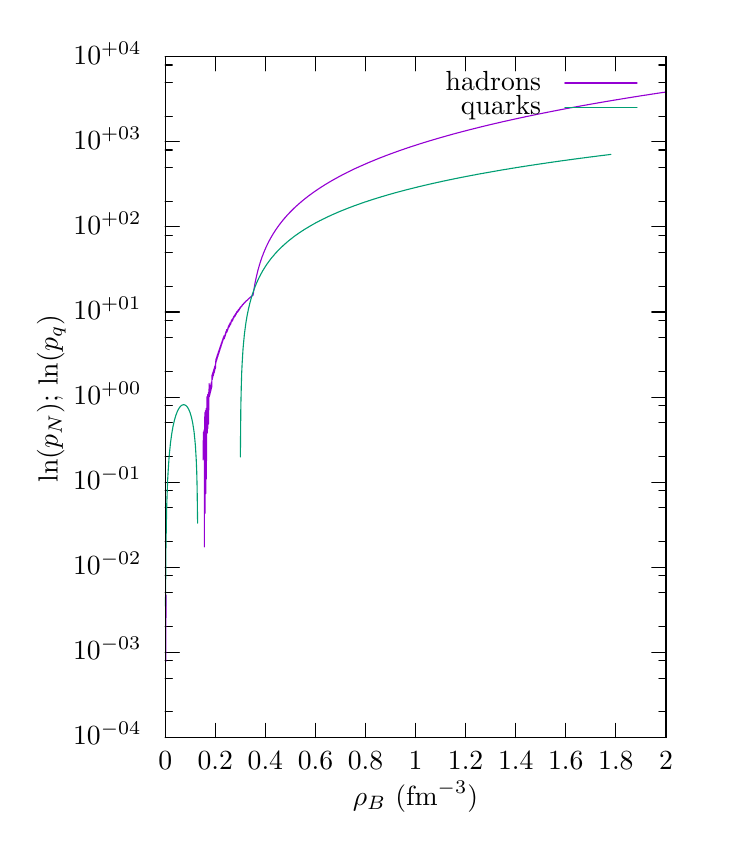
\begin{tikzpicture}[gnuplot]
%% generated with GNUPLOT 5.0p4 (Lua 5.2; terminal rev. 99, script rev. 100)
%% Thu Sep 29 16:33:16 2016
\path (0.000,0.000) rectangle (8.600,10.000);
\gpcolor{color=gp lt color border}
\gpsetlinetype{gp lt border}
\gpsetdashtype{gp dt solid}
\gpsetlinewidth{1.00}
\draw[gp path] (1.688,0.985)--(1.868,0.985);
\draw[gp path] (8.047,0.985)--(7.867,0.985);
\node[gp node right] at (1.504,0.985) {$10^{-04}$};
\draw[gp path] (1.688,1.310)--(1.778,1.310);
\draw[gp path] (8.047,1.310)--(7.957,1.310);
\draw[gp path] (1.688,1.740)--(1.778,1.740);
\draw[gp path] (8.047,1.740)--(7.957,1.740);
\draw[gp path] (1.688,1.961)--(1.778,1.961);
\draw[gp path] (8.047,1.961)--(7.957,1.961);
\draw[gp path] (1.688,2.066)--(1.868,2.066);
\draw[gp path] (8.047,2.066)--(7.867,2.066);
\node[gp node right] at (1.504,2.066) {$10^{-03}$};
\draw[gp path] (1.688,2.391)--(1.778,2.391);
\draw[gp path] (8.047,2.391)--(7.957,2.391);
\draw[gp path] (1.688,2.821)--(1.778,2.821);
\draw[gp path] (8.047,2.821)--(7.957,2.821);
\draw[gp path] (1.688,3.042)--(1.778,3.042);
\draw[gp path] (8.047,3.042)--(7.957,3.042);
\draw[gp path] (1.688,3.147)--(1.868,3.147);
\draw[gp path] (8.047,3.147)--(7.867,3.147);
\node[gp node right] at (1.504,3.147) {$10^{-02}$};
\draw[gp path] (1.688,3.472)--(1.778,3.472);
\draw[gp path] (8.047,3.472)--(7.957,3.472);
\draw[gp path] (1.688,3.902)--(1.778,3.902);
\draw[gp path] (8.047,3.902)--(7.957,3.902);
\draw[gp path] (1.688,4.123)--(1.778,4.123);
\draw[gp path] (8.047,4.123)--(7.957,4.123);
\draw[gp path] (1.688,4.227)--(1.868,4.227);
\draw[gp path] (8.047,4.227)--(7.867,4.227);
\node[gp node right] at (1.504,4.227) {$10^{-01}$};
\draw[gp path] (1.688,4.553)--(1.778,4.553);
\draw[gp path] (8.047,4.553)--(7.957,4.553);
\draw[gp path] (1.688,4.983)--(1.778,4.983);
\draw[gp path] (8.047,4.983)--(7.957,4.983);
\draw[gp path] (1.688,5.203)--(1.778,5.203);
\draw[gp path] (8.047,5.203)--(7.957,5.203);
\draw[gp path] (1.688,5.308)--(1.868,5.308);
\draw[gp path] (8.047,5.308)--(7.867,5.308);
\node[gp node right] at (1.504,5.308) {$10^{+00}$};
\draw[gp path] (1.688,5.633)--(1.778,5.633);
\draw[gp path] (8.047,5.633)--(7.957,5.633);
\draw[gp path] (1.688,6.063)--(1.778,6.063);
\draw[gp path] (8.047,6.063)--(7.957,6.063);
\draw[gp path] (1.688,6.284)--(1.778,6.284);
\draw[gp path] (8.047,6.284)--(7.957,6.284);
\draw[gp path] (1.688,6.389)--(1.868,6.389);
\draw[gp path] (8.047,6.389)--(7.867,6.389);
\node[gp node right] at (1.504,6.389) {$10^{+01}$};
\draw[gp path] (1.688,6.714)--(1.778,6.714);
\draw[gp path] (8.047,6.714)--(7.957,6.714);
\draw[gp path] (1.688,7.144)--(1.778,7.144);
\draw[gp path] (8.047,7.144)--(7.957,7.144);
\draw[gp path] (1.688,7.365)--(1.778,7.365);
\draw[gp path] (8.047,7.365)--(7.957,7.365);
\draw[gp path] (1.688,7.470)--(1.868,7.470);
\draw[gp path] (8.047,7.470)--(7.867,7.470);
\node[gp node right] at (1.504,7.470) {$10^{+02}$};
\draw[gp path] (1.688,7.795)--(1.778,7.795);
\draw[gp path] (8.047,7.795)--(7.957,7.795);
\draw[gp path] (1.688,8.225)--(1.778,8.225);
\draw[gp path] (8.047,8.225)--(7.957,8.225);
\draw[gp path] (1.688,8.446)--(1.778,8.446);
\draw[gp path] (8.047,8.446)--(7.957,8.446);
\draw[gp path] (1.688,8.550)--(1.868,8.550);
\draw[gp path] (8.047,8.550)--(7.867,8.550);
\node[gp node right] at (1.504,8.550) {$10^{+03}$};
\draw[gp path] (1.688,8.876)--(1.778,8.876);
\draw[gp path] (8.047,8.876)--(7.957,8.876);
\draw[gp path] (1.688,9.306)--(1.778,9.306);
\draw[gp path] (8.047,9.306)--(7.957,9.306);
\draw[gp path] (1.688,9.526)--(1.778,9.526);
\draw[gp path] (8.047,9.526)--(7.957,9.526);
\draw[gp path] (1.688,9.631)--(1.868,9.631);
\draw[gp path] (8.047,9.631)--(7.867,9.631);
\node[gp node right] at (1.504,9.631) {$10^{+04}$};
\draw[gp path] (1.688,0.985)--(1.688,1.165);
\draw[gp path] (1.688,9.631)--(1.688,9.451);
\node[gp node center] at (1.688,0.677) {$0$};
\draw[gp path] (2.324,0.985)--(2.324,1.165);
\draw[gp path] (2.324,9.631)--(2.324,9.451);
\node[gp node center] at (2.324,0.677) {$0.2$};
\draw[gp path] (2.960,0.985)--(2.960,1.165);
\draw[gp path] (2.960,9.631)--(2.960,9.451);
\node[gp node center] at (2.960,0.677) {$0.4$};
\draw[gp path] (3.596,0.985)--(3.596,1.165);
\draw[gp path] (3.596,9.631)--(3.596,9.451);
\node[gp node center] at (3.596,0.677) {$0.6$};
\draw[gp path] (4.232,0.985)--(4.232,1.165);
\draw[gp path] (4.232,9.631)--(4.232,9.451);
\node[gp node center] at (4.232,0.677) {$0.8$};
\draw[gp path] (4.868,0.985)--(4.868,1.165);
\draw[gp path] (4.868,9.631)--(4.868,9.451);
\node[gp node center] at (4.868,0.677) {$1$};
\draw[gp path] (5.503,0.985)--(5.503,1.165);
\draw[gp path] (5.503,9.631)--(5.503,9.451);
\node[gp node center] at (5.503,0.677) {$1.2$};
\draw[gp path] (6.139,0.985)--(6.139,1.165);
\draw[gp path] (6.139,9.631)--(6.139,9.451);
\node[gp node center] at (6.139,0.677) {$1.4$};
\draw[gp path] (6.775,0.985)--(6.775,1.165);
\draw[gp path] (6.775,9.631)--(6.775,9.451);
\node[gp node center] at (6.775,0.677) {$1.6$};
\draw[gp path] (7.411,0.985)--(7.411,1.165);
\draw[gp path] (7.411,9.631)--(7.411,9.451);
\node[gp node center] at (7.411,0.677) {$1.8$};
\draw[gp path] (8.047,0.985)--(8.047,1.165);
\draw[gp path] (8.047,9.631)--(8.047,9.451);
\node[gp node center] at (8.047,0.677) {$2$};
\draw[gp path] (1.688,9.631)--(1.688,0.985)--(8.047,0.985)--(8.047,9.631)--cycle;
\node[gp node center,rotate=-270] at (0.246,5.308) {$\ln(p_N)$; $\ln(p_q)$};
\node[gp node center] at (4.867,0.215) {$\rho_B$ ($\rm{fm}^{-3}$)};
\node[gp node right] at (6.579,9.297) {hadrons};
\gpcolor{rgb color={0.580,0.000,0.827}}
\draw[gp path] (6.763,9.297)--(7.679,9.297);
\draw[gp path] (1.695,1.949)--(1.698,2.796);
\draw[gp path] (2.170,4.510)--(2.172,4.863);
\draw[gp path] (2.179,4.561)--(2.181,4.893);
\draw[gp path] (2.185,3.406)--(2.187,4.616)--(2.189,4.925)--(2.191,5.111)--(2.193,3.832)%
  --(2.196,4.673)--(2.198,4.959)--(2.200,5.137)--(2.202,4.083)--(2.204,4.732)--(2.206,4.996)%
  --(2.208,5.165)--(2.210,4.268)--(2.213,4.792)--(2.215,5.034)--(2.217,5.195)--(2.219,5.315)%
  --(2.221,4.851)--(2.223,5.074)--(2.225,5.225)--(2.227,5.340)--(2.229,4.909)--(2.232,5.114)%
  --(2.234,5.257)--(2.236,5.367)--(2.238,4.967)--(2.240,5.155)--(2.242,5.289)--(2.244,5.394)%
  --(2.246,5.481)--(2.249,5.314)--(2.251,5.415)--(2.253,5.331)--(2.255,5.430)--(2.257,5.347)%
  --(2.259,5.444)--(2.261,5.364)--(2.263,5.458)--(2.266,5.381)--(2.268,5.473)--(2.270,5.398)%
  --(2.272,5.488)--(2.274,5.415)--(2.276,5.502)--(2.278,5.432)--(2.280,5.517)--(2.282,5.589)%
  --(2.285,5.532)--(2.287,5.603)--(2.289,5.547)--(2.291,5.616)--(2.293,5.562)--(2.295,5.629)%
  --(2.297,5.577)--(2.299,5.643)--(2.302,5.591)--(2.304,5.656)--(2.306,5.606)--(2.308,5.670)%
  --(2.310,5.621)--(2.312,5.683)--(2.314,5.636)--(2.316,5.697)--(2.318,5.651)--(2.321,5.710)%
  --(2.323,5.666)--(2.325,5.724)--(2.327,5.681)--(2.329,5.738)--(2.331,5.788)--(2.333,5.751)%
  --(2.335,5.801)--(2.338,5.765)--(2.340,5.814)--(2.342,5.778)--(2.344,5.826)--(2.346,5.792)%
  --(2.348,5.839)--(2.350,5.805)--(2.352,5.851)--(2.355,5.819)--(2.357,5.864)--(2.359,5.832)%
  --(2.361,5.876)--(2.363,5.846)--(2.365,5.889)--(2.367,5.859)--(2.369,5.901)--(2.371,5.872)%
  --(2.374,5.914)--(2.376,5.886)--(2.378,5.926)--(2.380,5.899)--(2.382,5.939)--(2.384,5.912)%
  --(2.386,5.951)--(2.388,5.925)--(2.391,5.964)--(2.393,5.939)--(2.395,5.976)--(2.397,5.952)%
  --(2.399,5.988)--(2.401,5.965)--(2.403,6.001)--(2.405,5.978)--(2.408,6.013)--(2.410,5.991)%
  --(2.412,6.025)--(2.414,6.004)--(2.416,6.037)--(2.418,6.016)--(2.420,6.050)--(2.422,6.029)%
  --(2.424,6.062)--(2.427,6.042)--(2.429,6.074)--(2.431,6.054)--(2.433,6.086)--(2.435,6.067)%
  --(2.437,6.048)--(2.439,6.080)--(2.441,6.061)--(2.444,6.092)--(2.446,6.074)--(2.448,6.104)%
  --(2.450,6.087)--(2.452,6.117)--(2.454,6.100)--(2.456,6.129)--(2.458,6.112)--(2.460,6.141)%
  --(2.463,6.125)--(2.465,6.153)--(2.467,6.138)--(2.469,6.166)--(2.471,6.150)--(2.473,6.135)%
  --(2.475,6.163)--(2.477,6.148)--(2.480,6.175)--(2.482,6.161)--(2.484,6.188)--(2.486,6.174)%
  --(2.488,6.200)--(2.490,6.186)--(2.492,6.212)--(2.494,6.199)--(2.497,6.224)--(2.499,6.212)%
  --(2.501,6.199)--(2.503,6.224)--(2.505,6.212)--(2.507,6.236)--(2.509,6.224)--(2.511,6.249)%
  --(2.513,6.237)--(2.516,6.225)--(2.518,6.250)--(2.520,6.238)--(2.522,6.262)--(2.524,6.251)%
  --(2.526,6.275)--(2.528,6.264)--(2.530,6.287)--(2.533,6.277)--(2.535,6.266)--(2.537,6.289)%
  --(2.539,6.279)--(2.541,6.302)--(2.543,6.292)--(2.545,6.282)--(2.547,6.305)--(2.550,6.296)%
  --(2.552,6.318)--(2.554,6.309)--(2.556,6.330)--(2.558,6.322)--(2.560,6.313)--(2.562,6.335)%
  --(2.564,6.326)--(2.566,6.347)--(2.569,6.339)--(2.571,6.331)--(2.573,6.352)--(2.575,6.344)%
  --(2.577,6.337)--(2.579,6.358)--(2.581,6.350)--(2.583,6.371)--(2.586,6.363)--(2.588,6.356)%
  --(2.590,6.377)--(2.592,6.370)--(2.594,6.390)--(2.596,6.383)--(2.598,6.377)--(2.600,6.397)%
  --(2.602,6.390)--(2.605,6.384)--(2.607,6.404)--(2.609,6.398)--(2.611,6.392)--(2.613,6.412)%
  --(2.615,6.406)--(2.617,6.401)--(2.619,6.420)--(2.622,6.415)--(2.624,6.410)--(2.626,6.429)%
  --(2.628,6.424)--(2.630,6.419)--(2.632,6.438)--(2.634,6.434)--(2.636,6.429)--(2.639,6.448)%
  --(2.641,6.438)--(2.643,6.445)--(2.645,6.452)--(2.647,6.449)--(2.649,6.456)--(2.651,6.452)%
  --(2.653,6.460)--(2.655,6.456)--(2.658,6.464)--(2.660,6.461)--(2.662,6.468)--(2.664,6.476)%
  --(2.666,6.473)--(2.668,6.481)--(2.670,6.478)--(2.672,6.486)--(2.675,6.484)--(2.677,6.482)%
  --(2.679,6.489)--(2.681,6.488)--(2.683,6.496)--(2.685,6.494)--(2.687,6.502)--(2.689,6.501)%
  --(2.691,6.500)--(2.694,6.508)--(2.696,6.507)--(2.698,6.506)--(2.700,6.514)--(2.702,6.514)%
  --(2.704,6.514)--(2.706,6.522)--(2.708,6.522)--(2.711,6.522)--(2.713,6.522)--(2.715,6.531)%
  --(2.717,6.532)--(2.719,6.532)--(2.721,6.533)--(2.723,6.534)--(2.725,6.536)--(2.728,6.537)%
  --(2.730,6.539)--(2.732,6.541)--(2.734,6.543)--(2.736,6.545)--(2.738,6.547)--(2.740,6.550)%
  --(2.742,6.552)--(2.744,6.555)--(2.747,6.558)--(2.749,6.561)--(2.751,6.559)--(2.753,6.562)%
  --(2.755,6.566)--(2.757,6.565)--(2.759,6.569)--(2.761,6.569)--(2.764,6.571)--(2.766,6.574)%
  --(2.768,6.577)--(2.770,6.577)--(2.772,6.578)--(2.774,6.580)--(2.776,6.582)--(2.778,6.584)%
  --(2.781,6.585)--(2.783,6.588)--(2.785,6.588)--(2.787,6.591)--(2.789,6.591)--(2.791,6.594)%
  --(2.793,6.595)--(2.795,6.597)--(2.797,6.598)--(2.800,6.600)--(2.802,6.601)--(2.804,6.605)%
  --(2.806,6.620)--(2.808,6.634)--(2.810,6.648)--(2.812,6.662)--(2.814,6.675)--(2.817,6.688)%
  --(2.819,6.700)--(2.821,6.712)--(2.823,6.724)--(2.825,6.736)--(2.827,6.747)--(2.829,6.759)%
  --(2.831,6.769)--(2.833,6.780)--(2.836,6.791)--(2.838,6.801)--(2.840,6.811)--(2.842,6.821)%
  --(2.844,6.830)--(2.846,6.840)--(2.848,6.849)--(2.850,6.858)--(2.853,6.867)--(2.855,6.876)%
  --(2.857,6.885)--(2.859,6.893)--(2.861,6.902)--(2.863,6.910)--(2.865,6.918)--(2.867,6.926)%
  --(2.870,6.934)--(2.872,6.942)--(2.874,6.949)--(2.876,6.957)--(2.878,6.964)--(2.880,6.971)%
  --(2.882,6.979)--(2.884,6.986)--(2.886,6.993)--(2.889,7.000)--(2.891,7.007)--(2.893,7.013)%
  --(2.895,7.020)--(2.897,7.027)--(2.899,7.033)--(2.901,7.040)--(2.903,7.046)--(2.906,7.052)%
  --(2.908,7.058)--(2.910,7.065)--(2.912,7.071)--(2.914,7.077)--(2.916,7.083)--(2.918,7.088)%
  --(2.920,7.094)--(2.923,7.100)--(2.925,7.106)--(2.927,7.111)--(2.929,7.117)--(2.931,7.122)%
  --(2.933,7.128)--(2.935,7.133)--(2.937,7.139)--(2.939,7.144)--(2.942,7.149)--(2.944,7.154)%
  --(2.946,7.159)--(2.948,7.164)--(2.950,7.170)--(2.952,7.175)--(2.954,7.179)--(2.956,7.184)%
  --(2.959,7.189)--(2.961,7.194)--(2.963,7.199)--(2.965,7.204)--(2.967,7.208)--(2.969,7.213)%
  --(2.971,7.218)--(2.973,7.222)--(2.975,7.227)--(2.978,7.231)--(2.980,7.236)--(2.982,7.240)%
  --(2.984,7.245)--(2.986,7.249)--(2.988,7.253)--(2.990,7.258)--(2.992,7.262)--(2.995,7.266)%
  --(2.997,7.270)--(2.999,7.274)--(3.001,7.279)--(3.003,7.283)--(3.005,7.287)--(3.007,7.291)%
  --(3.009,7.295)--(3.012,7.299)--(3.014,7.303)--(3.016,7.307)--(3.018,7.311)--(3.020,7.315)%
  --(3.022,7.318)--(3.024,7.322)--(3.026,7.326)--(3.028,7.330)--(3.031,7.334)--(3.033,7.337)%
  --(3.035,7.341)--(3.037,7.345)--(3.039,7.348)--(3.041,7.352)--(3.043,7.356)--(3.045,7.359)%
  --(3.048,7.363)--(3.050,7.366)--(3.052,7.370)--(3.054,7.373)--(3.056,7.377)--(3.058,7.380)%
  --(3.060,7.384)--(3.062,7.387)--(3.064,7.391)--(3.067,7.394)--(3.069,7.397)--(3.071,7.401)%
  --(3.073,7.404)--(3.075,7.407)--(3.077,7.411)--(3.079,7.414)--(3.081,7.417)--(3.084,7.420)%
  --(3.086,7.424)--(3.088,7.427)--(3.090,7.430)--(3.092,7.433)--(3.094,7.436)--(3.096,7.439)%
  --(3.098,7.442)--(3.101,7.446)--(3.103,7.449)--(3.105,7.452)--(3.107,7.455)--(3.109,7.458)%
  --(3.111,7.461)--(3.113,7.464)--(3.115,7.467)--(3.117,7.470)--(3.120,7.473)--(3.122,7.476)%
  --(3.124,7.479)--(3.126,7.482)--(3.128,7.484)--(3.130,7.487)--(3.132,7.490)--(3.134,7.493)%
  --(3.137,7.496)--(3.139,7.499)--(3.141,7.502)--(3.143,7.504)--(3.145,7.507)--(3.147,7.510)%
  --(3.149,7.513)--(3.151,7.515)--(3.154,7.518)--(3.156,7.521)--(3.158,7.524)--(3.160,7.526)%
  --(3.162,7.529)--(3.164,7.532)--(3.166,7.534)--(3.168,7.537)--(3.170,7.540)--(3.173,7.542)%
  --(3.175,7.545)--(3.177,7.548)--(3.179,7.550)--(3.181,7.553)--(3.183,7.555)--(3.185,7.558)%
  --(3.187,7.561)--(3.190,7.563)--(3.192,7.566)--(3.194,7.568)--(3.196,7.571)--(3.198,7.573)%
  --(3.200,7.576)--(3.202,7.578)--(3.204,7.581)--(3.206,7.583)--(3.209,7.586)--(3.211,7.588)%
  --(3.213,7.590)--(3.215,7.593)--(3.217,7.595)--(3.219,7.598)--(3.221,7.600)--(3.223,7.602)%
  --(3.226,7.605)--(3.228,7.607)--(3.230,7.610)--(3.232,7.612)--(3.234,7.614)--(3.236,7.617)%
  --(3.238,7.619)--(3.240,7.621)--(3.243,7.624)--(3.245,7.626)--(3.247,7.628)--(3.249,7.630)%
  --(3.251,7.633)--(3.253,7.635)--(3.255,7.637)--(3.257,7.640)--(3.259,7.642)--(3.262,7.644)%
  --(3.264,7.646)--(3.266,7.648)--(3.268,7.651)--(3.270,7.653)--(3.272,7.655)--(3.274,7.657)%
  --(3.276,7.659)--(3.279,7.662)--(3.281,7.664)--(3.283,7.666)--(3.285,7.668)--(3.287,7.670)%
  --(3.289,7.672)--(3.291,7.675)--(3.293,7.677)--(3.295,7.679)--(3.298,7.681)--(3.300,7.683)%
  --(3.302,7.685)--(3.304,7.687)--(3.306,7.689)--(3.308,7.691)--(3.310,7.693)--(3.312,7.696)%
  --(3.315,7.698)--(3.317,7.700)--(3.319,7.702)--(3.321,7.704)--(3.323,7.706)--(3.325,7.708)%
  --(3.327,7.710)--(3.329,7.712)--(3.332,7.714)--(3.334,7.716)--(3.336,7.718)--(3.338,7.720)%
  --(3.340,7.722)--(3.342,7.724)--(3.344,7.726)--(3.346,7.728)--(3.348,7.730)--(3.351,7.732)%
  --(3.353,7.734)--(3.355,7.736)--(3.357,7.737)--(3.359,7.739)--(3.361,7.741)--(3.363,7.743)%
  --(3.365,7.745)--(3.368,7.747)--(3.370,7.749)--(3.372,7.751)--(3.374,7.753)--(3.376,7.755)%
  --(3.378,7.756)--(3.380,7.758)--(3.382,7.760)--(3.385,7.762)--(3.387,7.764)--(3.389,7.766)%
  --(3.391,7.768)--(3.393,7.770)--(3.395,7.771)--(3.397,7.773)--(3.399,7.775)--(3.401,7.777)%
  --(3.404,7.779)--(3.406,7.780)--(3.408,7.782)--(3.410,7.784)--(3.412,7.786)--(3.414,7.788)%
  --(3.416,7.789)--(3.418,7.791)--(3.421,7.793)--(3.423,7.795)--(3.425,7.797)--(3.427,7.798)%
  --(3.429,7.800)--(3.431,7.802)--(3.433,7.804)--(3.435,7.805)--(3.437,7.807)--(3.440,7.809)%
  --(3.442,7.811)--(3.444,7.812)--(3.446,7.814)--(3.448,7.816)--(3.450,7.817)--(3.452,7.819)%
  --(3.454,7.821)--(3.457,7.823)--(3.459,7.824)--(3.461,7.826)--(3.463,7.828)--(3.465,7.829)%
  --(3.467,7.831)--(3.469,7.833)--(3.471,7.834)--(3.474,7.836)--(3.476,7.838)--(3.478,7.839)%
  --(3.480,7.841)--(3.482,7.843)--(3.484,7.844)--(3.486,7.846)--(3.488,7.848)--(3.490,7.849)%
  --(3.493,7.851)--(3.495,7.853)--(3.497,7.854)--(3.499,7.856)--(3.501,7.857)--(3.503,7.859)%
  --(3.505,7.861)--(3.507,7.862)--(3.510,7.864)--(3.512,7.865)--(3.514,7.867)--(3.516,7.869)%
  --(3.518,7.870)--(3.520,7.872)--(3.522,7.873)--(3.524,7.875)--(3.527,7.877)--(3.529,7.878)%
  --(3.531,7.880)--(3.533,7.881)--(3.535,7.883)--(3.537,7.884)--(3.539,7.886)--(3.541,7.887)%
  --(3.543,7.889)--(3.546,7.891)--(3.548,7.892)--(3.550,7.894)--(3.552,7.895)--(3.554,7.897)%
  --(3.556,7.898)--(3.558,7.900)--(3.560,7.901)--(3.563,7.903)--(3.565,7.904)--(3.567,7.906)%
  --(3.569,7.907)--(3.571,7.909)--(3.573,7.910)--(3.575,7.912)--(3.577,7.913)--(3.579,7.915)%
  --(3.582,7.916)--(3.584,7.918)--(3.586,7.919)--(3.588,7.921)--(3.590,7.922)--(3.592,7.924)%
  --(3.594,7.925)--(3.596,7.927)--(3.599,7.928)--(3.601,7.929)--(3.603,7.931)--(3.605,7.932)%
  --(3.607,7.934)--(3.609,7.935)--(3.611,7.937)--(3.613,7.938)--(3.616,7.940)--(3.618,7.941)%
  --(3.620,7.942)--(3.622,7.944)--(3.624,7.945)--(3.626,7.947)--(3.628,7.948)--(3.630,7.950)%
  --(3.632,7.951)--(3.635,7.952)--(3.637,7.954)--(3.639,7.955)--(3.641,7.957)--(3.643,7.958)%
  --(3.645,7.959)--(3.647,7.961)--(3.649,7.962)--(3.652,7.964)--(3.654,7.965)--(3.656,7.966)%
  --(3.658,7.968)--(3.660,7.969)--(3.662,7.970)--(3.664,7.972)--(3.666,7.973)--(3.668,7.975)%
  --(3.671,7.976)--(3.673,7.977)--(3.675,7.979)--(3.677,7.980)--(3.679,7.981)--(3.681,7.983)%
  --(3.683,7.984)--(3.685,7.985)--(3.688,7.987)--(3.690,7.988)--(3.692,7.989)--(3.694,7.991)%
  --(3.696,7.992)--(3.698,7.993)--(3.700,7.995)--(3.702,7.996)--(3.705,7.997)--(3.707,7.999)%
  --(3.709,8.000)--(3.711,8.001)--(3.713,8.003)--(3.715,8.004)--(3.717,8.005)--(3.719,8.007)%
  --(3.721,8.008)--(3.724,8.009)--(3.726,8.011)--(3.728,8.012)--(3.730,8.013)--(3.732,8.014)%
  --(3.734,8.016)--(3.736,8.017)--(3.738,8.018)--(3.741,8.020)--(3.743,8.021)--(3.745,8.022)%
  --(3.747,8.023)--(3.749,8.025)--(3.751,8.026)--(3.753,8.027)--(3.755,8.029)--(3.758,8.030)%
  --(3.760,8.031)--(3.762,8.032)--(3.764,8.034)--(3.766,8.035)--(3.768,8.036)--(3.770,8.037)%
  --(3.772,8.039)--(3.774,8.040)--(3.777,8.041)--(3.779,8.042)--(3.781,8.044)--(3.783,8.045)%
  --(3.785,8.046)--(3.787,8.047)--(3.789,8.049)--(3.791,8.050)--(3.794,8.051)--(3.796,8.052)%
  --(3.798,8.053)--(3.800,8.055)--(3.802,8.056)--(3.804,8.057)--(3.806,8.058)--(3.808,8.060)%
  --(3.810,8.061)--(3.813,8.062)--(3.815,8.063)--(3.817,8.064)--(3.819,8.066)--(3.821,8.067)%
  --(3.823,8.068)--(3.825,8.069)--(3.827,8.070)--(3.830,8.072)--(3.832,8.073)--(3.834,8.074)%
  --(3.836,8.075)--(3.838,8.076)--(3.840,8.078)--(3.842,8.079)--(3.844,8.080)--(3.847,8.081)%
  --(3.849,8.082)--(3.851,8.083)--(3.853,8.085)--(3.855,8.086)--(3.857,8.087)--(3.859,8.088)%
  --(3.861,8.089)--(3.863,8.090)--(3.866,8.092)--(3.868,8.093)--(3.870,8.094)--(3.872,8.095)%
  --(3.874,8.096)--(3.876,8.097)--(3.878,8.099)--(3.880,8.100)--(3.883,8.101)--(3.885,8.102)%
  --(3.887,8.103)--(3.889,8.104)--(3.891,8.105)--(3.893,8.107)--(3.895,8.108)--(3.897,8.109)%
  --(3.900,8.110)--(3.902,8.111)--(3.904,8.112)--(3.906,8.113)--(3.908,8.115)--(3.910,8.116)%
  --(3.912,8.117)--(3.914,8.118)--(3.916,8.119)--(3.919,8.120)--(3.921,8.121)--(3.923,8.122)%
  --(3.925,8.124)--(3.927,8.125)--(3.929,8.126)--(3.931,8.127)--(3.933,8.128)--(3.936,8.129)%
  --(3.938,8.130)--(3.940,8.131)--(3.942,8.132)--(3.944,8.133)--(3.946,8.135)--(3.948,8.136)%
  --(3.950,8.137)--(3.952,8.138)--(3.955,8.139)--(3.957,8.140)--(3.959,8.141)--(3.961,8.142)%
  --(3.963,8.143)--(3.965,8.144)--(3.967,8.145)--(3.969,8.147)--(3.972,8.148)--(3.974,8.149)%
  --(3.976,8.150)--(3.978,8.151)--(3.980,8.152)--(3.982,8.153)--(3.984,8.154)--(3.986,8.155)%
  --(3.989,8.156)--(3.991,8.157)--(3.993,8.158)--(3.995,8.159)--(3.997,8.160)--(3.999,8.162)%
  --(4.001,8.163)--(4.003,8.164)--(4.005,8.165)--(4.008,8.166)--(4.010,8.167)--(4.012,8.168)%
  --(4.014,8.169)--(4.016,8.170)--(4.018,8.171)--(4.020,8.172)--(4.022,8.173)--(4.025,8.174)%
  --(4.027,8.175)--(4.029,8.176)--(4.031,8.177)--(4.033,8.178)--(4.035,8.179)--(4.037,8.180)%
  --(4.039,8.181)--(4.041,8.182)--(4.044,8.183)--(4.046,8.184)--(4.048,8.186)--(4.050,8.187)%
  --(4.052,8.188)--(4.054,8.189)--(4.056,8.190)--(4.058,8.191)--(4.061,8.192)--(4.063,8.193)%
  --(4.065,8.194)--(4.067,8.195)--(4.069,8.196)--(4.071,8.197)--(4.073,8.198)--(4.075,8.199)%
  --(4.078,8.200)--(4.080,8.201)--(4.082,8.202)--(4.084,8.203)--(4.086,8.204)--(4.088,8.205)%
  --(4.090,8.206)--(4.092,8.207)--(4.094,8.208)--(4.097,8.209)--(4.099,8.210)--(4.101,8.211)%
  --(4.103,8.212)--(4.105,8.213)--(4.107,8.214)--(4.109,8.215)--(4.111,8.216)--(4.114,8.217)%
  --(4.116,8.218)--(4.118,8.219)--(4.120,8.220)--(4.122,8.221)--(4.124,8.222)--(4.126,8.223)%
  --(4.128,8.224)--(4.131,8.225)--(4.133,8.225)--(4.135,8.226)--(4.137,8.227)--(4.139,8.228)%
  --(4.141,8.229)--(4.143,8.230)--(4.145,8.231)--(4.147,8.232)--(4.150,8.233)--(4.152,8.234)%
  --(4.154,8.235)--(4.156,8.236)--(4.158,8.237)--(4.160,8.238)--(4.162,8.239)--(4.164,8.240)%
  --(4.167,8.241)--(4.169,8.242)--(4.171,8.243)--(4.173,8.244)--(4.175,8.245)--(4.177,8.246)%
  --(4.179,8.247)--(4.181,8.248)--(4.183,8.249)--(4.186,8.249)--(4.188,8.250)--(4.190,8.251)%
  --(4.192,8.252)--(4.194,8.253)--(4.196,8.254)--(4.198,8.255)--(4.200,8.256)--(4.203,8.257)%
  --(4.205,8.258)--(4.207,8.259)--(4.209,8.260)--(4.211,8.261)--(4.213,8.262)--(4.215,8.263)%
  --(4.217,8.264)--(4.220,8.264)--(4.222,8.265)--(4.224,8.266)--(4.226,8.267)--(4.228,8.268)%
  --(4.230,8.269)--(4.232,8.270)--(4.234,8.271)--(4.236,8.272)--(4.239,8.273)--(4.241,8.274)%
  --(4.243,8.275)--(4.245,8.275)--(4.247,8.276)--(4.249,8.277)--(4.251,8.278)--(4.253,8.279)%
  --(4.256,8.280)--(4.258,8.281)--(4.260,8.282)--(4.262,8.283)--(4.264,8.284)--(4.266,8.285)%
  --(4.268,8.285)--(4.270,8.286)--(4.273,8.287)--(4.275,8.288)--(4.277,8.289)--(4.279,8.290)%
  --(4.281,8.291)--(4.283,8.292)--(4.285,8.293)--(4.287,8.294)--(4.289,8.294)--(4.292,8.295)%
  --(4.294,8.296)--(4.296,8.297)--(4.298,8.298)--(4.300,8.299)--(4.302,8.300)--(4.304,8.301)%
  --(4.306,8.302)--(4.309,8.302)--(4.311,8.303)--(4.313,8.304)--(4.315,8.305)--(4.317,8.306)%
  --(4.319,8.307)--(4.321,8.308)--(4.323,8.309)--(4.325,8.309)--(4.328,8.310)--(4.330,8.311)%
  --(4.332,8.312)--(4.334,8.313)--(4.336,8.314)--(4.338,8.315)--(4.340,8.316)--(4.342,8.316)%
  --(4.345,8.317)--(4.347,8.318)--(4.349,8.319)--(4.351,8.320)--(4.353,8.321)--(4.355,8.322)%
  --(4.357,8.322)--(4.359,8.323)--(4.362,8.324)--(4.364,8.325)--(4.366,8.326)--(4.368,8.327)%
  --(4.370,8.328)--(4.372,8.328)--(4.374,8.329)--(4.376,8.330)--(4.378,8.331)--(4.381,8.332)%
  --(4.383,8.333)--(4.385,8.334)--(4.387,8.334)--(4.389,8.335)--(4.391,8.336)--(4.393,8.337)%
  --(4.395,8.338)--(4.398,8.339)--(4.400,8.339)--(4.402,8.340)--(4.404,8.341)--(4.406,8.342)%
  --(4.408,8.343)--(4.410,8.344)--(4.412,8.345)--(4.414,8.345)--(4.417,8.346)--(4.419,8.347)%
  --(4.421,8.348)--(4.423,8.349)--(4.425,8.350)--(4.427,8.350)--(4.429,8.351)--(4.431,8.352)%
  --(4.434,8.353)--(4.436,8.354)--(4.438,8.355)--(4.440,8.355)--(4.442,8.356)--(4.444,8.357)%
  --(4.446,8.358)--(4.448,8.359)--(4.451,8.359)--(4.453,8.360)--(4.455,8.361)--(4.457,8.362)%
  --(4.459,8.363)--(4.461,8.364)--(4.463,8.364)--(4.465,8.365)--(4.467,8.366)--(4.470,8.367)%
  --(4.472,8.368)--(4.474,8.368)--(4.476,8.369)--(4.478,8.370)--(4.480,8.371)--(4.482,8.372)%
  --(4.484,8.372)--(4.487,8.373)--(4.489,8.374)--(4.491,8.375)--(4.493,8.376)--(4.495,8.377)%
  --(4.497,8.377)--(4.499,8.378)--(4.501,8.379)--(4.504,8.380)--(4.506,8.381)--(4.508,8.381)%
  --(4.510,8.382)--(4.512,8.383)--(4.514,8.384)--(4.516,8.385)--(4.518,8.385)--(4.520,8.386)%
  --(4.523,8.387)--(4.525,8.388)--(4.527,8.388)--(4.529,8.389)--(4.531,8.390)--(4.533,8.391)%
  --(4.535,8.392)--(4.537,8.392)--(4.540,8.393)--(4.542,8.394)--(4.544,8.395)--(4.546,8.396)%
  --(4.548,8.396)--(4.550,8.397)--(4.552,8.398)--(4.554,8.399)--(4.556,8.400)--(4.559,8.400)%
  --(4.561,8.401)--(4.563,8.402)--(4.565,8.403)--(4.567,8.403)--(4.569,8.404)--(4.571,8.405)%
  --(4.573,8.406)--(4.576,8.407)--(4.578,8.407)--(4.580,8.408)--(4.582,8.409)--(4.584,8.410)%
  --(4.586,8.410)--(4.588,8.411)--(4.590,8.412)--(4.593,8.413)--(4.595,8.413)--(4.597,8.414)%
  --(4.599,8.415)--(4.601,8.416)--(4.603,8.417)--(4.605,8.417)--(4.607,8.418)--(4.609,8.419)%
  --(4.612,8.420)--(4.614,8.420)--(4.616,8.421)--(4.618,8.422)--(4.620,8.423)--(4.622,8.423)%
  --(4.624,8.424)--(4.626,8.425)--(4.629,8.426)--(4.631,8.426)--(4.633,8.427)--(4.635,8.428)%
  --(4.637,8.429)--(4.639,8.429)--(4.641,8.430)--(4.643,8.431)--(4.646,8.432)--(4.648,8.432)%
  --(4.650,8.433)--(4.652,8.434)--(4.654,8.435)--(4.656,8.435)--(4.658,8.436)--(4.660,8.437)%
  --(4.662,8.438)--(4.665,8.438)--(4.667,8.439)--(4.669,8.440)--(4.671,8.441)--(4.673,8.441)%
  --(4.675,8.442)--(4.677,8.443)--(4.679,8.444)--(4.682,8.444)--(4.684,8.445)--(4.686,8.446)%
  --(4.688,8.447)--(4.690,8.447)--(4.692,8.448)--(4.694,8.449)--(4.696,8.450)--(4.698,8.450)%
  --(4.701,8.451)--(4.703,8.452)--(4.705,8.452)--(4.707,8.453)--(4.709,8.454)--(4.711,8.455)%
  --(4.713,8.455)--(4.715,8.456)--(4.718,8.457)--(4.720,8.458)--(4.722,8.458)--(4.724,8.459)%
  --(4.726,8.460)--(4.728,8.460)--(4.730,8.461)--(4.732,8.462)--(4.735,8.463)--(4.737,8.463)%
  --(4.739,8.464)--(4.741,8.465)--(4.743,8.466)--(4.745,8.466)--(4.747,8.467)--(4.749,8.468)%
  --(4.751,8.468)--(4.754,8.469)--(4.756,8.470)--(4.758,8.471)--(4.760,8.471)--(4.762,8.472)%
  --(4.764,8.473)--(4.766,8.473)--(4.768,8.474)--(4.771,8.475)--(4.773,8.476)--(4.775,8.476)%
  --(4.777,8.477)--(4.779,8.478)--(4.781,8.478)--(4.783,8.479)--(4.785,8.480)--(4.787,8.481)%
  --(4.790,8.481)--(4.792,8.482)--(4.794,8.483)--(4.796,8.483)--(4.798,8.484)--(4.800,8.485)%
  --(4.802,8.485)--(4.804,8.486)--(4.807,8.487)--(4.809,8.488)--(4.811,8.488)--(4.813,8.489)%
  --(4.815,8.490)--(4.817,8.490)--(4.819,8.491)--(4.821,8.492)--(4.824,8.492)--(4.826,8.493)%
  --(4.828,8.494)--(4.830,8.495)--(4.832,8.495)--(4.834,8.496)--(4.836,8.497)--(4.838,8.497)%
  --(4.840,8.498)--(4.843,8.499)--(4.845,8.499)--(4.847,8.500)--(4.849,8.501)--(4.851,8.501)%
  --(4.853,8.502)--(4.855,8.503)--(4.857,8.504)--(4.860,8.504)--(4.862,8.505)--(4.864,8.506)%
  --(4.866,8.506)--(4.868,8.507)--(4.870,8.508)--(4.872,8.508)--(4.874,8.509)--(4.877,8.510)%
  --(4.879,8.510)--(4.881,8.511)--(4.883,8.512)--(4.885,8.512)--(4.887,8.513)--(4.889,8.514)%
  --(4.891,8.514)--(4.893,8.515)--(4.896,8.516)--(4.898,8.516)--(4.900,8.517)--(4.902,8.518)%
  --(4.904,8.519)--(4.906,8.519)--(4.908,8.520)--(4.910,8.521)--(4.913,8.521)--(4.915,8.522)%
  --(4.917,8.523)--(4.919,8.523)--(4.921,8.524)--(4.923,8.525)--(4.925,8.525)--(4.927,8.526)%
  --(4.929,8.527)--(4.932,8.527)--(4.934,8.528)--(4.936,8.529)--(4.938,8.529)--(4.940,8.530)%
  --(4.942,8.531)--(4.944,8.531)--(4.946,8.532)--(4.949,8.533)--(4.951,8.533)--(4.953,8.534)%
  --(4.955,8.535)--(4.957,8.535)--(4.959,8.536)--(4.961,8.537)--(4.963,8.537)--(4.966,8.538)%
  --(4.968,8.539)--(4.970,8.539)--(4.972,8.540)--(4.974,8.541)--(4.976,8.541)--(4.978,8.542)%
  --(4.980,8.543)--(4.982,8.543)--(4.985,8.544)--(4.987,8.544)--(4.989,8.545)--(4.991,8.546)%
  --(4.993,8.546)--(4.995,8.547)--(4.997,8.548)--(4.999,8.548)--(5.002,8.549)--(5.004,8.550)%
  --(5.006,8.550)--(5.008,8.551)--(5.010,8.552)--(5.012,8.552)--(5.014,8.553)--(5.016,8.554)%
  --(5.019,8.554)--(5.021,8.555)--(5.023,8.556)--(5.025,8.556)--(5.027,8.557)--(5.029,8.557)%
  --(5.031,8.558)--(5.033,8.559)--(5.035,8.559)--(5.038,8.560)--(5.040,8.561)--(5.042,8.561)%
  --(5.044,8.562)--(5.046,8.563)--(5.048,8.563)--(5.050,8.564)--(5.052,8.565)--(5.055,8.565)%
  --(5.057,8.566)--(5.059,8.566)--(5.061,8.567)--(5.063,8.568)--(5.065,8.568)--(5.067,8.569)%
  --(5.069,8.570)--(5.071,8.570)--(5.074,8.571)--(5.076,8.572)--(5.078,8.572)--(5.080,8.573)%
  --(5.082,8.573)--(5.084,8.574)--(5.086,8.575)--(5.088,8.575)--(5.091,8.576)--(5.093,8.577)%
  --(5.095,8.577)--(5.097,8.578)--(5.099,8.578)--(5.101,8.579)--(5.103,8.580)--(5.105,8.580)%
  --(5.108,8.581)--(5.110,8.582)--(5.112,8.582)--(5.114,8.583)--(5.116,8.583)--(5.118,8.584)%
  --(5.120,8.585)--(5.122,8.585)--(5.124,8.586)--(5.127,8.587)--(5.129,8.587)--(5.131,8.588)%
  --(5.133,8.588)--(5.135,8.589)--(5.137,8.590)--(5.139,8.590)--(5.141,8.591)--(5.144,8.592)%
  --(5.146,8.592)--(5.148,8.593)--(5.150,8.593)--(5.152,8.594)--(5.154,8.595)--(5.156,8.595)%
  --(5.158,8.596)--(5.160,8.597)--(5.163,8.597)--(5.165,8.598)--(5.167,8.598)--(5.169,8.599)%
  --(5.171,8.600)--(5.173,8.600)--(5.175,8.601)--(5.177,8.601)--(5.180,8.602)--(5.182,8.603)%
  --(5.184,8.603)--(5.186,8.604)--(5.188,8.604)--(5.190,8.605)--(5.192,8.606)--(5.194,8.606)%
  --(5.197,8.607)--(5.199,8.608)--(5.201,8.608)--(5.203,8.609)--(5.205,8.609)--(5.207,8.610)%
  --(5.209,8.611)--(5.211,8.611)--(5.213,8.612)--(5.216,8.612)--(5.218,8.613)--(5.220,8.614)%
  --(5.222,8.614)--(5.224,8.615)--(5.226,8.615)--(5.228,8.616)--(5.230,8.617)--(5.233,8.617)%
  --(5.235,8.618)--(5.237,8.618)--(5.239,8.619)--(5.241,8.620)--(5.243,8.620)--(5.245,8.621)%
  --(5.247,8.621)--(5.250,8.622)--(5.252,8.623)--(5.254,8.623)--(5.256,8.624)--(5.258,8.624)%
  --(5.260,8.625)--(5.262,8.626)--(5.264,8.626)--(5.266,8.627)--(5.269,8.627)--(5.271,8.628)%
  --(5.273,8.629)--(5.275,8.629)--(5.277,8.630)--(5.279,8.630)--(5.281,8.631)--(5.283,8.631)%
  --(5.286,8.632)--(5.288,8.633)--(5.290,8.633)--(5.292,8.634)--(5.294,8.634)--(5.296,8.635)%
  --(5.298,8.636)--(5.300,8.636)--(5.302,8.637)--(5.305,8.637)--(5.307,8.638)--(5.309,8.639)%
  --(5.311,8.639)--(5.313,8.640)--(5.315,8.640)--(5.317,8.641)--(5.319,8.641)--(5.322,8.642)%
  --(5.324,8.643)--(5.326,8.643)--(5.328,8.644)--(5.330,8.644)--(5.332,8.645)--(5.334,8.646)%
  --(5.336,8.646)--(5.339,8.647)--(5.341,8.647)--(5.343,8.648)--(5.345,8.648)--(5.347,8.649)%
  --(5.349,8.650)--(5.351,8.650)--(5.353,8.651)--(5.355,8.651)--(5.358,8.652)--(5.360,8.652)%
  --(5.362,8.653)--(5.364,8.654)--(5.366,8.654)--(5.368,8.655)--(5.370,8.655)--(5.372,8.656)%
  --(5.375,8.656)--(5.377,8.657)--(5.379,8.658)--(5.381,8.658)--(5.383,8.659)--(5.385,8.659)%
  --(5.387,8.660)--(5.389,8.660)--(5.392,8.661)--(5.394,8.662)--(5.396,8.662)--(5.398,8.663)%
  --(5.400,8.663)--(5.402,8.664)--(5.404,8.664)--(5.406,8.665)--(5.408,8.666)--(5.411,8.666)%
  --(5.413,8.667)--(5.415,8.667)--(5.417,8.668)--(5.419,8.668)--(5.421,8.669)--(5.423,8.670)%
  --(5.425,8.670)--(5.428,8.671)--(5.430,8.671)--(5.432,8.672)--(5.434,8.672)--(5.436,8.673)%
  --(5.438,8.674)--(5.440,8.674)--(5.442,8.675)--(5.444,8.675)--(5.447,8.676)--(5.449,8.676)%
  --(5.451,8.677)--(5.453,8.677)--(5.455,8.678)--(5.457,8.679)--(5.459,8.679)--(5.461,8.680)%
  --(5.464,8.680)--(5.466,8.681)--(5.468,8.681)--(5.470,8.682)--(5.472,8.682)--(5.474,8.683)%
  --(5.476,8.684)--(5.478,8.684)--(5.481,8.685)--(5.483,8.685)--(5.485,8.686)--(5.487,8.686)%
  --(5.489,8.687)--(5.491,8.687)--(5.493,8.688)--(5.495,8.689)--(5.497,8.689)--(5.500,8.690)%
  --(5.502,8.690)--(5.504,8.691)--(5.506,8.691)--(5.508,8.692)--(5.510,8.692)--(5.512,8.693)%
  --(5.514,8.693)--(5.517,8.694)--(5.519,8.695)--(5.521,8.695)--(5.523,8.696)--(5.525,8.696)%
  --(5.527,8.697)--(5.529,8.697)--(5.531,8.698)--(5.533,8.698)--(5.536,8.699)--(5.538,8.700)%
  --(5.540,8.700)--(5.542,8.701)--(5.544,8.701)--(5.546,8.702)--(5.548,8.702)--(5.550,8.703)%
  --(5.553,8.703)--(5.555,8.704)--(5.557,8.704)--(5.559,8.705)--(5.561,8.705)--(5.563,8.706)%
  --(5.565,8.707)--(5.567,8.707)--(5.570,8.708)--(5.572,8.708)--(5.574,8.709)--(5.576,8.709)%
  --(5.578,8.710)--(5.580,8.710)--(5.582,8.711)--(5.584,8.711)--(5.586,8.712)--(5.589,8.712)%
  --(5.591,8.713)--(5.593,8.714)--(5.595,8.714)--(5.597,8.715)--(5.599,8.715)--(5.601,8.716)%
  --(5.603,8.716)--(5.606,8.717)--(5.608,8.717)--(5.610,8.718)--(5.612,8.718)--(5.614,8.719)%
  --(5.616,8.719)--(5.618,8.720)--(5.620,8.721)--(5.623,8.721)--(5.625,8.722)--(5.627,8.722)%
  --(5.629,8.723)--(5.631,8.723)--(5.633,8.724)--(5.635,8.724)--(5.637,8.725)--(5.639,8.725)%
  --(5.642,8.726)--(5.644,8.726)--(5.646,8.727)--(5.648,8.727)--(5.650,8.728)--(5.652,8.728)%
  --(5.654,8.729)--(5.656,8.729)--(5.659,8.730)--(5.661,8.731)--(5.663,8.731)--(5.665,8.732)%
  --(5.667,8.732)--(5.669,8.733)--(5.671,8.733)--(5.673,8.734)--(5.675,8.734)--(5.678,8.735)%
  --(5.680,8.735)--(5.682,8.736)--(5.684,8.736)--(5.686,8.737)--(5.688,8.737)--(5.690,8.738)%
  --(5.692,8.738)--(5.695,8.739)--(5.697,8.739)--(5.699,8.740)--(5.701,8.740)--(5.703,8.741)%
  --(5.705,8.742)--(5.707,8.742)--(5.709,8.743)--(5.712,8.743)--(5.714,8.744)--(5.716,8.744)%
  --(5.718,8.745)--(5.720,8.745)--(5.722,8.746)--(5.724,8.746)--(5.726,8.747)--(5.728,8.747)%
  --(5.731,8.748)--(5.733,8.748)--(5.735,8.749)--(5.737,8.749)--(5.739,8.750)--(5.741,8.750)%
  --(5.743,8.751)--(5.745,8.751)--(5.748,8.752)--(5.750,8.752)--(5.752,8.753)--(5.754,8.753)%
  --(5.756,8.754)--(5.758,8.754)--(5.760,8.755)--(5.762,8.755)--(5.764,8.756)--(5.767,8.756)%
  --(5.769,8.757)--(5.771,8.757)--(5.773,8.758)--(5.775,8.758)--(5.777,8.759)--(5.779,8.759)%
  --(5.781,8.760)--(5.784,8.761)--(5.786,8.761)--(5.788,8.762)--(5.790,8.762)--(5.792,8.763)%
  --(5.794,8.763)--(5.796,8.764)--(5.798,8.764)--(5.801,8.765)--(5.803,8.765)--(5.805,8.766)%
  --(5.807,8.766)--(5.809,8.767)--(5.811,8.767)--(5.813,8.768)--(5.815,8.768)--(5.817,8.769)%
  --(5.820,8.769)--(5.822,8.770)--(5.824,8.770)--(5.826,8.771)--(5.828,8.771)--(5.830,8.772)%
  --(5.832,8.772)--(5.834,8.773)--(5.837,8.773)--(5.839,8.774)--(5.841,8.774)--(5.843,8.775)%
  --(5.845,8.775)--(5.847,8.776)--(5.849,8.776)--(5.851,8.777)--(5.854,8.777)--(5.856,8.778)%
  --(5.858,8.778)--(5.860,8.779)--(5.862,8.779)--(5.864,8.780)--(5.866,8.780)--(5.868,8.781)%
  --(5.870,8.781)--(5.873,8.782)--(5.875,8.782)--(5.877,8.783)--(5.879,8.783)--(5.881,8.784)%
  --(5.883,8.784)--(5.885,8.785)--(5.887,8.785)--(5.890,8.786)--(5.892,8.786)--(5.894,8.787)%
  --(5.896,8.787)--(5.898,8.787)--(5.900,8.788)--(5.902,8.788)--(5.904,8.789)--(5.906,8.789)%
  --(5.909,8.790)--(5.911,8.790)--(5.913,8.791)--(5.915,8.791)--(5.917,8.792)--(5.919,8.792)%
  --(5.921,8.793)--(5.923,8.793)--(5.926,8.794)--(5.928,8.794)--(5.930,8.795)--(5.932,8.795)%
  --(5.934,8.796)--(5.936,8.796)--(5.938,8.797)--(5.940,8.797)--(5.943,8.798)--(5.945,8.798)%
  --(5.947,8.799)--(5.949,8.799)--(5.951,8.800)--(5.953,8.800)--(5.955,8.801)--(5.957,8.801)%
  --(5.959,8.802)--(5.962,8.802)--(5.964,8.803)--(5.966,8.803)--(5.968,8.804)--(5.970,8.804)%
  --(5.972,8.805)--(5.974,8.805)--(5.976,8.806)--(5.979,8.806)--(5.981,8.806)--(5.983,8.807)%
  --(5.985,8.807)--(5.987,8.808)--(5.989,8.808)--(5.991,8.809)--(5.993,8.809)--(5.996,8.810)%
  --(5.998,8.810)--(6.000,8.811)--(6.002,8.811)--(6.004,8.812)--(6.006,8.812)--(6.008,8.813)%
  --(6.010,8.813)--(6.012,8.814)--(6.015,8.814)--(6.017,8.815)--(6.019,8.815)--(6.021,8.816)%
  --(6.023,8.816)--(6.025,8.817)--(6.027,8.817)--(6.029,8.817)--(6.032,8.818)--(6.034,8.818)%
  --(6.036,8.819)--(6.038,8.819)--(6.040,8.820)--(6.042,8.820)--(6.044,8.821)--(6.046,8.821)%
  --(6.048,8.822)--(6.051,8.822)--(6.053,8.823)--(6.055,8.823)--(6.057,8.824)--(6.059,8.824)%
  --(6.061,8.825)--(6.063,8.825)--(6.065,8.826)--(6.068,8.826)--(6.070,8.826)--(6.072,8.827)%
  --(6.074,8.827)--(6.076,8.828)--(6.078,8.828)--(6.080,8.829)--(6.082,8.829)--(6.085,8.830)%
  --(6.087,8.830)--(6.089,8.831)--(6.091,8.831)--(6.093,8.832)--(6.095,8.832)--(6.097,8.833)%
  --(6.099,8.833)--(6.101,8.833)--(6.104,8.834)--(6.106,8.834)--(6.108,8.835)--(6.110,8.835)%
  --(6.112,8.836)--(6.114,8.836)--(6.116,8.837)--(6.118,8.837)--(6.121,8.838)--(6.123,8.838)%
  --(6.125,8.839)--(6.127,8.839)--(6.129,8.840)--(6.131,8.840)--(6.133,8.840)--(6.135,8.841)%
  --(6.137,8.841)--(6.140,8.842)--(6.142,8.842)--(6.144,8.843)--(6.146,8.843)--(6.148,8.844)%
  --(6.150,8.844)--(6.152,8.845)--(6.154,8.845)--(6.157,8.846)--(6.159,8.846)--(6.161,8.846)%
  --(6.163,8.847)--(6.165,8.847)--(6.167,8.848)--(6.169,8.848)--(6.171,8.849)--(6.174,8.849)%
  --(6.176,8.850)--(6.178,8.850)--(6.180,8.851)--(6.182,8.851)--(6.184,8.852)--(6.186,8.852)%
  --(6.188,8.852)--(6.190,8.853)--(6.193,8.853)--(6.195,8.854)--(6.197,8.854)--(6.199,8.855)%
  --(6.201,8.855)--(6.203,8.856)--(6.205,8.856)--(6.207,8.857)--(6.210,8.857)--(6.212,8.857)%
  --(6.214,8.858)--(6.216,8.858)--(6.218,8.859)--(6.220,8.859)--(6.222,8.860)--(6.224,8.860)%
  --(6.227,8.861)--(6.229,8.861)--(6.231,8.862)--(6.233,8.862)--(6.235,8.862)--(6.237,8.863)%
  --(6.239,8.863)--(6.241,8.864)--(6.243,8.864)--(6.246,8.865)--(6.248,8.865)--(6.250,8.866)%
  --(6.252,8.866)--(6.254,8.866)--(6.256,8.867)--(6.258,8.867)--(6.260,8.868)--(6.263,8.868)%
  --(6.265,8.869)--(6.267,8.869)--(6.269,8.870)--(6.271,8.870)--(6.273,8.870)--(6.275,8.871)%
  --(6.277,8.871)--(6.279,8.872)--(6.282,8.872)--(6.284,8.873)--(6.286,8.873)--(6.288,8.874)%
  --(6.290,8.874)--(6.292,8.875)--(6.294,8.875)--(6.296,8.875)--(6.299,8.876)--(6.301,8.876)%
  --(6.303,8.877)--(6.305,8.877)--(6.307,8.878)--(6.309,8.878)--(6.311,8.879)--(6.313,8.879)%
  --(6.316,8.879)--(6.318,8.880)--(6.320,8.880)--(6.322,8.881)--(6.324,8.881)--(6.326,8.882)%
  --(6.328,8.882)--(6.330,8.882)--(6.332,8.883)--(6.335,8.883)--(6.337,8.884)--(6.339,8.884)%
  --(6.341,8.885)--(6.343,8.885)--(6.345,8.886)--(6.347,8.886)--(6.349,8.886)--(6.352,8.887)%
  --(6.354,8.887)--(6.356,8.888)--(6.358,8.888)--(6.360,8.889)--(6.362,8.889)--(6.364,8.890)%
  --(6.366,8.890)--(6.369,8.890)--(6.371,8.891)--(6.373,8.891)--(6.375,8.892)--(6.377,8.892)%
  --(6.379,8.893)--(6.381,8.893)--(6.383,8.893)--(6.385,8.894)--(6.388,8.894)--(6.390,8.895)%
  --(6.392,8.895)--(6.394,8.896)--(6.396,8.896)--(6.398,8.897)--(6.400,8.897)--(6.402,8.897)%
  --(6.405,8.898)--(6.407,8.898)--(6.409,8.899)--(6.411,8.899)--(6.413,8.900)--(6.415,8.900)%
  --(6.417,8.900)--(6.419,8.901)--(6.421,8.901)--(6.424,8.902)--(6.426,8.902)--(6.428,8.903)%
  --(6.430,8.903)--(6.432,8.903)--(6.434,8.904)--(6.436,8.904)--(6.438,8.905)--(6.441,8.905)%
  --(6.443,8.906)--(6.445,8.906)--(6.447,8.906)--(6.449,8.907)--(6.451,8.907)--(6.453,8.908)%
  --(6.455,8.908)--(6.458,8.909)--(6.460,8.909)--(6.462,8.909)--(6.464,8.910)--(6.466,8.910)%
  --(6.468,8.911)--(6.470,8.911)--(6.472,8.912)--(6.474,8.912)--(6.477,8.912)--(6.479,8.913)%
  --(6.481,8.913)--(6.483,8.914)--(6.485,8.914)--(6.487,8.915)--(6.489,8.915)--(6.491,8.915)%
  --(6.494,8.916)--(6.496,8.916)--(6.498,8.917)--(6.500,8.917)--(6.502,8.918)--(6.504,8.918)%
  --(6.506,8.918)--(6.508,8.919)--(6.510,8.919)--(6.513,8.920)--(6.515,8.920)--(6.517,8.920)%
  --(6.519,8.921)--(6.521,8.921)--(6.523,8.922)--(6.525,8.922)--(6.527,8.923)--(6.530,8.923)%
  --(6.532,8.923)--(6.534,8.924)--(6.536,8.924)--(6.538,8.925)--(6.540,8.925)--(6.542,8.926)%
  --(6.544,8.926)--(6.547,8.926)--(6.549,8.927)--(6.551,8.927)--(6.553,8.928)--(6.555,8.928)%
  --(6.557,8.928)--(6.559,8.929)--(6.561,8.929)--(6.563,8.930)--(6.566,8.930)--(6.568,8.931)%
  --(6.570,8.931)--(6.572,8.931)--(6.574,8.932)--(6.576,8.932)--(6.578,8.933)--(6.580,8.933)%
  --(6.583,8.933)--(6.585,8.934)--(6.587,8.934)--(6.589,8.935)--(6.591,8.935)--(6.593,8.936)%
  --(6.595,8.936)--(6.597,8.936)--(6.600,8.937)--(6.602,8.937)--(6.604,8.938)--(6.606,8.938)%
  --(6.608,8.938)--(6.610,8.939)--(6.612,8.939)--(6.614,8.940)--(6.616,8.940)--(6.619,8.941)%
  --(6.621,8.941)--(6.623,8.941)--(6.625,8.942)--(6.627,8.942)--(6.629,8.943)--(6.631,8.943)%
  --(6.633,8.943)--(6.636,8.944)--(6.638,8.944)--(6.640,8.945)--(6.642,8.945)--(6.644,8.945)%
  --(6.646,8.946)--(6.648,8.946)--(6.650,8.947)--(6.652,8.947)--(6.655,8.948)--(6.657,8.948)%
  --(6.659,8.948)--(6.661,8.949)--(6.663,8.949)--(6.665,8.950)--(6.667,8.950)--(6.669,8.950)%
  --(6.672,8.951)--(6.674,8.951)--(6.676,8.952)--(6.678,8.952)--(6.680,8.952)--(6.682,8.953)%
  --(6.684,8.953)--(6.686,8.954)--(6.689,8.954)--(6.691,8.954)--(6.693,8.955)--(6.695,8.955)%
  --(6.697,8.956)--(6.699,8.956)--(6.701,8.957)--(6.703,8.957)--(6.705,8.957)--(6.708,8.958)%
  --(6.710,8.958)--(6.712,8.959)--(6.714,8.959)--(6.716,8.959)--(6.718,8.960)--(6.720,8.960)%
  --(6.722,8.961)--(6.725,8.961)--(6.727,8.961)--(6.729,8.962)--(6.731,8.962)--(6.733,8.963)%
  --(6.735,8.963)--(6.737,8.963)--(6.739,8.964)--(6.742,8.964)--(6.744,8.965)--(6.746,8.965)%
  --(6.748,8.965)--(6.750,8.966)--(6.752,8.966)--(6.754,8.967)--(6.756,8.967)--(6.758,8.967)%
  --(6.761,8.968)--(6.763,8.968)--(6.765,8.969)--(6.767,8.969)--(6.769,8.969)--(6.771,8.970)%
  --(6.773,8.970)--(6.775,8.971)--(6.778,8.971)--(6.780,8.971)--(6.782,8.972)--(6.784,8.972)%
  --(6.786,8.973)--(6.788,8.973)--(6.790,8.973)--(6.792,8.974)--(6.794,8.974)--(6.797,8.975)%
  --(6.799,8.975)--(6.801,8.975)--(6.803,8.976)--(6.805,8.976)--(6.807,8.977)--(6.809,8.977)%
  --(6.811,8.977)--(6.814,8.978)--(6.816,8.978)--(6.818,8.979)--(6.820,8.979)--(6.822,8.979)%
  --(6.824,8.980)--(6.826,8.980)--(6.828,8.981)--(6.831,8.981)--(6.833,8.981)--(6.835,8.982)%
  --(6.837,8.982)--(6.839,8.982)--(6.841,8.983)--(6.843,8.983)--(6.845,8.984)--(6.847,8.984)%
  --(6.850,8.984)--(6.852,8.985)--(6.854,8.985)--(6.856,8.986)--(6.858,8.986)--(6.860,8.986)%
  --(6.862,8.987)--(6.864,8.987)--(6.867,8.988)--(6.869,8.988)--(6.871,8.988)--(6.873,8.989)%
  --(6.875,8.989)--(6.877,8.990)--(6.879,8.990)--(6.881,8.990)--(6.883,8.991)--(6.886,8.991)%
  --(6.888,8.992)--(6.890,8.992)--(6.892,8.992)--(6.894,8.993)--(6.896,8.993)--(6.898,8.993)%
  --(6.900,8.994)--(6.903,8.994)--(6.905,8.995)--(6.907,8.995)--(6.909,8.995)--(6.911,8.996)%
  --(6.913,8.996)--(6.915,8.997)--(6.917,8.997)--(6.920,8.997)--(6.922,8.998)--(6.924,8.998)%
  --(6.926,8.999)--(6.928,8.999)--(6.930,8.999)--(6.932,9.000)--(6.934,9.000)--(6.936,9.000)%
  --(6.939,9.001)--(6.941,9.001)--(6.943,9.002)--(6.945,9.002)--(6.947,9.002)--(6.949,9.003)%
  --(6.951,9.003)--(6.953,9.004)--(6.956,9.004)--(6.958,9.004)--(6.960,9.005)--(6.962,9.005)%
  --(6.964,9.005)--(6.966,9.006)--(6.968,9.006)--(6.970,9.007)--(6.973,9.007)--(6.975,9.007)%
  --(6.977,9.008)--(6.979,9.008)--(6.981,9.009)--(6.983,9.009)--(6.985,9.009)--(6.987,9.010)%
  --(6.989,9.010)--(6.992,9.010)--(6.994,9.011)--(6.996,9.011)--(6.998,9.012)--(7.000,9.012)%
  --(7.002,9.012)--(7.004,9.013)--(7.006,9.013)--(7.009,9.013)--(7.011,9.014)--(7.013,9.014)%
  --(7.015,9.015)--(7.017,9.015)--(7.019,9.015)--(7.021,9.016)--(7.023,9.016)--(7.025,9.017)%
  --(7.028,9.017)--(7.030,9.017)--(7.032,9.018)--(7.034,9.018)--(7.036,9.018)--(7.038,9.019)%
  --(7.040,9.019)--(7.042,9.020)--(7.045,9.020)--(7.047,9.020)--(7.049,9.021)--(7.051,9.021)%
  --(7.053,9.021)--(7.055,9.022)--(7.057,9.022)--(7.059,9.023)--(7.062,9.023)--(7.064,9.023)%
  --(7.066,9.024)--(7.068,9.024)--(7.070,9.024)--(7.072,9.025)--(7.074,9.025)--(7.076,9.026)%
  --(7.078,9.026)--(7.081,9.026)--(7.083,9.027)--(7.085,9.027)--(7.087,9.027)--(7.089,9.028)%
  --(7.091,9.028)--(7.093,9.029)--(7.095,9.029)--(7.098,9.029)--(7.100,9.030)--(7.102,9.030)%
  --(7.104,9.030)--(7.106,9.031)--(7.108,9.031)--(7.110,9.032)--(7.112,9.032)--(7.115,9.032)%
  --(7.117,9.033)--(7.119,9.033)--(7.121,9.033)--(7.123,9.034)--(7.125,9.034)--(7.127,9.035)%
  --(7.129,9.035)--(7.131,9.035)--(7.134,9.036)--(7.136,9.036)--(7.138,9.036)--(7.140,9.037)%
  --(7.142,9.037)--(7.144,9.037)--(7.146,9.038)--(7.148,9.038)--(7.151,9.039)--(7.153,9.039)%
  --(7.155,9.039)--(7.157,9.040)--(7.159,9.040)--(7.161,9.040)--(7.163,9.041)--(7.165,9.041)%
  --(7.167,9.042)--(7.170,9.042)--(7.172,9.042)--(7.174,9.043)--(7.176,9.043)--(7.178,9.043)%
  --(7.180,9.044)--(7.182,9.044)--(7.184,9.044)--(7.187,9.045)--(7.189,9.045)--(7.191,9.046)%
  --(7.193,9.046)--(7.195,9.046)--(7.197,9.047)--(7.199,9.047)--(7.201,9.047)--(7.204,9.048)%
  --(7.206,9.048)--(7.208,9.049)--(7.210,9.049)--(7.212,9.049)--(7.214,9.050)--(7.216,9.050)%
  --(7.218,9.050)--(7.220,9.051)--(7.223,9.051)--(7.225,9.051)--(7.227,9.052)--(7.229,9.052)%
  --(7.231,9.053)--(7.233,9.053)--(7.235,9.053)--(7.237,9.054)--(7.240,9.054)--(7.242,9.054)%
  --(7.244,9.055)--(7.246,9.055)--(7.248,9.055)--(7.250,9.056)--(7.252,9.056)--(7.254,9.057)%
  --(7.256,9.057)--(7.259,9.057)--(7.261,9.058)--(7.263,9.058)--(7.265,9.058)--(7.267,9.059)%
  --(7.269,9.059)--(7.271,9.059)--(7.273,9.060)--(7.276,9.060)--(7.278,9.061)--(7.280,9.061)%
  --(7.282,9.061)--(7.284,9.062)--(7.286,9.062)--(7.288,9.062)--(7.290,9.063)--(7.293,9.063)%
  --(7.295,9.063)--(7.297,9.064)--(7.299,9.064)--(7.301,9.064)--(7.303,9.065)--(7.305,9.065)%
  --(7.307,9.066)--(7.309,9.066)--(7.312,9.066)--(7.314,9.067)--(7.316,9.067)--(7.318,9.067)%
  --(7.320,9.068)--(7.322,9.068)--(7.324,9.068)--(7.326,9.069)--(7.329,9.069)--(7.331,9.069)%
  --(7.333,9.070)--(7.335,9.070)--(7.337,9.071)--(7.339,9.071)--(7.341,9.071)--(7.343,9.072)%
  --(7.346,9.072)--(7.348,9.072)--(7.350,9.073)--(7.352,9.073)--(7.354,9.073)--(7.356,9.074)%
  --(7.358,9.074)--(7.360,9.074)--(7.362,9.075)--(7.365,9.075)--(7.367,9.076)--(7.369,9.076)%
  --(7.371,9.076)--(7.373,9.077)--(7.375,9.077)--(7.377,9.077)--(7.379,9.078)--(7.382,9.078)%
  --(7.384,9.078)--(7.386,9.079)--(7.388,9.079)--(7.390,9.079)--(7.392,9.080)--(7.394,9.080)%
  --(7.396,9.081)--(7.398,9.081)--(7.401,9.081)--(7.403,9.082)--(7.405,9.082)--(7.407,9.082)%
  --(7.409,9.083)--(7.411,9.083)--(7.413,9.083)--(7.415,9.084)--(7.418,9.084)--(7.420,9.084)%
  --(7.422,9.085)--(7.424,9.085)--(7.426,9.085)--(7.428,9.086)--(7.430,9.086)--(7.432,9.086)%
  --(7.435,9.087)--(7.437,9.087)--(7.439,9.088)--(7.441,9.088)--(7.443,9.088)--(7.445,9.089)%
  --(7.447,9.089)--(7.449,9.089)--(7.451,9.090)--(7.454,9.090)--(7.456,9.090)--(7.458,9.091)%
  --(7.460,9.091)--(7.462,9.091)--(7.464,9.092)--(7.466,9.092)--(7.468,9.092)--(7.471,9.093)%
  --(7.473,9.093)--(7.475,9.093)--(7.477,9.094)--(7.479,9.094)--(7.481,9.095)--(7.483,9.095)%
  --(7.485,9.095)--(7.488,9.096)--(7.490,9.096)--(7.492,9.096)--(7.494,9.097)--(7.496,9.097)%
  --(7.498,9.097)--(7.500,9.098)--(7.502,9.098)--(7.504,9.098)--(7.507,9.099)--(7.509,9.099)%
  --(7.511,9.099)--(7.513,9.100)--(7.515,9.100)--(7.517,9.100)--(7.519,9.101)--(7.521,9.101)%
  --(7.524,9.101)--(7.526,9.102)--(7.528,9.102)--(7.530,9.102)--(7.532,9.103)--(7.534,9.103)%
  --(7.536,9.103)--(7.538,9.104)--(7.540,9.104)--(7.543,9.105)--(7.545,9.105)--(7.547,9.105)%
  --(7.549,9.106)--(7.551,9.106)--(7.553,9.106)--(7.555,9.107)--(7.557,9.107)--(7.560,9.107)%
  --(7.562,9.108)--(7.564,9.108)--(7.566,9.108)--(7.568,9.109)--(7.570,9.109)--(7.572,9.109)%
  --(7.574,9.110)--(7.577,9.110)--(7.579,9.110)--(7.581,9.111)--(7.583,9.111)--(7.585,9.111)%
  --(7.587,9.112)--(7.589,9.112)--(7.591,9.112)--(7.593,9.113)--(7.596,9.113)--(7.598,9.113)%
  --(7.600,9.114)--(7.602,9.114)--(7.604,9.114)--(7.606,9.115)--(7.608,9.115)--(7.610,9.115)%
  --(7.613,9.116)--(7.615,9.116)--(7.617,9.116)--(7.619,9.117)--(7.621,9.117)--(7.623,9.117)%
  --(7.625,9.118)--(7.627,9.118)--(7.629,9.119)--(7.632,9.119)--(7.634,9.119)--(7.636,9.120)%
  --(7.638,9.120)--(7.640,9.120)--(7.642,9.121)--(7.644,9.121)--(7.646,9.121)--(7.649,9.122)%
  --(7.651,9.122)--(7.653,9.122)--(7.655,9.123)--(7.657,9.123)--(7.659,9.123)--(7.661,9.124)%
  --(7.663,9.124)--(7.666,9.124)--(7.668,9.125)--(7.670,9.125)--(7.672,9.125)--(7.674,9.126)%
  --(7.676,9.126)--(7.678,9.126)--(7.680,9.127)--(7.682,9.127)--(7.685,9.127)--(7.687,9.128)%
  --(7.689,9.128)--(7.691,9.128)--(7.693,9.129)--(7.695,9.129)--(7.697,9.129)--(7.699,9.130)%
  --(7.702,9.130)--(7.704,9.130)--(7.706,9.131)--(7.708,9.131)--(7.710,9.131)--(7.712,9.132)%
  --(7.714,9.132)--(7.716,9.132)--(7.719,9.133)--(7.721,9.133)--(7.723,9.133)--(7.725,9.134)%
  --(7.727,9.134)--(7.729,9.134)--(7.731,9.135)--(7.733,9.135)--(7.735,9.135)--(7.738,9.136)%
  --(7.740,9.136)--(7.742,9.136)--(7.744,9.137)--(7.746,9.137)--(7.748,9.137)--(7.750,9.138)%
  --(7.752,9.138)--(7.755,9.138)--(7.757,9.139)--(7.759,9.139)--(7.761,9.139)--(7.763,9.140)%
  --(7.765,9.140)--(7.767,9.140)--(7.769,9.141)--(7.771,9.141)--(7.774,9.141)--(7.776,9.142)%
  --(7.778,9.142)--(7.780,9.142)--(7.782,9.143)--(7.784,9.143)--(7.786,9.143)--(7.788,9.144)%
  --(7.791,9.144)--(7.793,9.144)--(7.795,9.145)--(7.797,9.145)--(7.799,9.145)--(7.801,9.145)%
  --(7.803,9.146)--(7.805,9.146)--(7.808,9.146)--(7.810,9.147)--(7.812,9.147)--(7.814,9.147)%
  --(7.816,9.148)--(7.818,9.148)--(7.820,9.148)--(7.822,9.149)--(7.824,9.149)--(7.827,9.149)%
  --(7.829,9.150)--(7.831,9.150)--(7.833,9.150)--(7.835,9.151)--(7.837,9.151)--(7.839,9.151)%
  --(7.841,9.152)--(7.844,9.152)--(7.846,9.152)--(7.848,9.153)--(7.850,9.153)--(7.852,9.153)%
  --(7.854,9.154)--(7.856,9.154)--(7.858,9.154)--(7.861,9.155)--(7.863,9.155)--(7.865,9.155)%
  --(7.867,9.156)--(7.869,9.156)--(7.871,9.156)--(7.873,9.157)--(7.875,9.157)--(7.877,9.157)%
  --(7.880,9.158)--(7.882,9.158)--(7.884,9.158)--(7.886,9.159)--(7.888,9.159)--(7.890,9.159)%
  --(7.892,9.159)--(7.894,9.160)--(7.897,9.160)--(7.899,9.160)--(7.901,9.161)--(7.903,9.161)%
  --(7.905,9.161)--(7.907,9.162)--(7.909,9.162)--(7.911,9.162)--(7.913,9.163)--(7.916,9.163)%
  --(7.918,9.163)--(7.920,9.164)--(7.922,9.164)--(7.924,9.164)--(7.926,9.165)--(7.928,9.165)%
  --(7.930,9.165)--(7.933,9.166)--(7.935,9.166)--(7.937,9.166)--(7.939,9.167)--(7.941,9.167)%
  --(7.943,9.167)--(7.945,9.168)--(7.947,9.168)--(7.950,9.168)--(7.952,9.169)--(7.954,9.169)%
  --(7.956,9.169)--(7.958,9.169)--(7.960,9.170)--(7.962,9.170)--(7.964,9.170)--(7.966,9.171)%
  --(7.969,9.171)--(7.971,9.171)--(7.973,9.172)--(7.975,9.172)--(7.977,9.172)--(7.979,9.173)%
  --(7.981,9.173)--(7.983,9.173)--(7.986,9.174)--(7.988,9.174)--(7.990,9.174)--(7.992,9.175)%
  --(7.994,9.175)--(7.996,9.175)--(7.998,9.176)--(8.000,9.176)--(8.002,9.176)--(8.005,9.176)%
  --(8.007,9.177)--(8.009,9.177)--(8.011,9.177)--(8.013,9.178)--(8.015,9.178)--(8.017,9.178)%
  --(8.019,9.179)--(8.022,9.179)--(8.024,9.179)--(8.026,9.180)--(8.028,9.180)--(8.030,9.180)%
  --(8.032,9.181)--(8.034,9.181)--(8.036,9.181)--(8.039,9.182)--(8.041,9.182)--(8.043,9.182)%
  --(8.045,9.182)--(8.047,9.183);
\gpcolor{color=gp lt color border}
\node[gp node right] at (6.579,8.989) {quarks};
\gpcolor{rgb color={0.000,0.620,0.451}}
\draw[gp path] (6.763,8.989)--(7.679,8.989);
\draw[gp path] (1.691,2.650)--(1.697,3.395)--(1.703,3.741)--(1.708,3.967)--(1.714,4.133)%
  --(1.719,4.262)--(1.725,4.368)--(1.731,4.458)--(1.736,4.534)--(1.742,4.601)--(1.748,4.659)%
  --(1.753,4.712)--(1.759,4.759)--(1.765,4.801)--(1.770,4.840)--(1.776,4.875)--(1.782,4.907)%
  --(1.787,4.937)--(1.793,4.964)--(1.799,4.989)--(1.804,5.012)--(1.810,5.033)--(1.816,5.053)%
  --(1.821,5.070)--(1.827,5.088)--(1.833,5.103)--(1.838,5.117)--(1.844,5.130)--(1.850,5.142)%
  --(1.855,5.153)--(1.861,5.162)--(1.867,5.172)--(1.872,5.179)--(1.878,5.186)--(1.884,5.192)%
  --(1.889,5.198)--(1.895,5.202)--(1.901,5.206)--(1.906,5.208)--(1.912,5.210)--(1.918,5.211)%
  --(1.923,5.212)--(1.929,5.211)--(1.935,5.209)--(1.940,5.207)--(1.946,5.204)--(1.952,5.199)%
  --(1.957,5.194)--(1.963,5.188)--(1.969,5.181)--(1.974,5.173)--(1.980,5.163)--(1.986,5.153)%
  --(1.991,5.140)--(1.997,5.128)--(2.003,5.112)--(2.008,5.096)--(2.014,5.076)--(2.020,5.056)%
  --(2.025,5.033)--(2.031,5.006)--(2.037,4.978)--(2.042,4.945)--(2.048,4.909)--(2.054,4.866)%
  --(2.059,4.817)--(2.065,4.759)--(2.071,4.693)--(2.076,4.608)--(2.082,4.505)--(2.088,4.360)%
  --(2.093,4.150)--(2.099,3.708);
\draw[gp path] (2.642,4.547)--(2.648,5.189)--(2.654,5.451)--(2.659,5.618)--(2.665,5.741)%
  --(2.671,5.839)--(2.676,5.920)--(2.682,5.989)--(2.688,6.050)--(2.693,6.103)--(2.699,6.151)%
  --(2.705,6.195)--(2.710,6.235)--(2.716,6.272)--(2.722,6.307)--(2.727,6.339)--(2.733,6.369)%
  --(2.739,6.397)--(2.744,6.424)--(2.750,6.449)--(2.756,6.473)--(2.761,6.496)--(2.767,6.518)%
  --(2.773,6.539)--(2.778,6.559)--(2.784,6.579)--(2.790,6.597)--(2.795,6.615)--(2.801,6.632)%
  --(2.807,6.649)--(2.812,6.665)--(2.818,6.681)--(2.824,6.696)--(2.829,6.711)--(2.835,6.725)%
  --(2.841,6.739)--(2.846,6.752)--(2.852,6.766)--(2.858,6.778)--(2.863,6.791)--(2.869,6.803)%
  --(2.875,6.815)--(2.880,6.827)--(2.886,6.838)--(2.892,6.849)--(2.897,6.860)--(2.903,6.871)%
  --(2.909,6.881)--(2.914,6.891)--(2.920,6.901)--(2.925,6.911)--(2.931,6.921)--(2.937,6.930)%
  --(2.942,6.939)--(2.948,6.948)--(2.954,6.957)--(2.959,6.966)--(2.965,6.975)--(2.971,6.983)%
  --(2.976,6.992)--(2.982,7.000)--(2.988,7.008)--(2.993,7.016)--(2.999,7.024)--(3.005,7.032)%
  --(3.010,7.039)--(3.016,7.047)--(3.022,7.054)--(3.027,7.061)--(3.033,7.069)--(3.039,7.076)%
  --(3.044,7.083)--(3.050,7.090)--(3.056,7.096)--(3.061,7.103)--(3.067,7.110)--(3.073,7.116)%
  --(3.078,7.123)--(3.084,7.129)--(3.090,7.136)--(3.095,7.142)--(3.101,7.148)--(3.107,7.154)%
  --(3.112,7.160)--(3.118,7.166)--(3.124,7.172)--(3.129,7.178)--(3.135,7.183)--(3.141,7.189)%
  --(3.146,7.195)--(3.152,7.200)--(3.158,7.206)--(3.163,7.211)--(3.169,7.217)--(3.175,7.222)%
  --(3.180,7.227)--(3.186,7.233)--(3.192,7.238)--(3.197,7.243)--(3.203,7.248)--(3.209,7.253)%
  --(3.214,7.258)--(3.220,7.263)--(3.226,7.268)--(3.231,7.273)--(3.237,7.278)--(3.243,7.282)%
  --(3.248,7.287)--(3.254,7.292)--(3.260,7.297)--(3.265,7.301)--(3.271,7.306)--(3.277,7.310)%
  --(3.282,7.315)--(3.288,7.319)--(3.294,7.324)--(3.299,7.328)--(3.305,7.332)--(3.311,7.337)%
  --(3.316,7.341)--(3.322,7.345)--(3.327,7.349)--(3.333,7.354)--(3.339,7.358)--(3.344,7.362)%
  --(3.350,7.366)--(3.356,7.370)--(3.361,7.374)--(3.367,7.378)--(3.373,7.382)--(3.378,7.386)%
  --(3.384,7.390)--(3.390,7.394)--(3.395,7.398)--(3.401,7.401)--(3.407,7.405)--(3.412,7.409)%
  --(3.418,7.413)--(3.424,7.416)--(3.429,7.420)--(3.435,7.424)--(3.441,7.427)--(3.446,7.431)%
  --(3.452,7.435)--(3.458,7.438)--(3.463,7.442)--(3.469,7.445)--(3.475,7.449)--(3.480,7.452)%
  --(3.486,7.456)--(3.492,7.459)--(3.497,7.463)--(3.503,7.466)--(3.509,7.469)--(3.514,7.473)%
  --(3.520,7.476)--(3.526,7.479)--(3.531,7.483)--(3.537,7.486)--(3.543,7.489)--(3.548,7.492)%
  --(3.554,7.496)--(3.560,7.499)--(3.565,7.502)--(3.571,7.505)--(3.577,7.508)--(3.582,7.511)%
  --(3.588,7.515)--(3.594,7.518)--(3.599,7.521)--(3.605,7.524)--(3.611,7.527)--(3.616,7.530)%
  --(3.622,7.533)--(3.628,7.536)--(3.633,7.539)--(3.639,7.542)--(3.645,7.545)--(3.650,7.548)%
  --(3.656,7.551)--(3.662,7.553)--(3.667,7.556)--(3.673,7.559)--(3.679,7.562)--(3.684,7.565)%
  --(3.690,7.568)--(3.696,7.570)--(3.701,7.573)--(3.707,7.576)--(3.713,7.579)--(3.718,7.582)%
  --(3.724,7.584)--(3.729,7.587)--(3.735,7.590)--(3.741,7.592)--(3.746,7.595)--(3.752,7.598)%
  --(3.758,7.600)--(3.763,7.603)--(3.769,7.606)--(3.775,7.608)--(3.780,7.611)--(3.786,7.614)%
  --(3.792,7.616)--(3.797,7.619)--(3.803,7.621)--(3.809,7.624)--(3.814,7.626)--(3.820,7.629)%
  --(3.826,7.631)--(3.831,7.634)--(3.837,7.636)--(3.843,7.639)--(3.848,7.641)--(3.854,7.644)%
  --(3.860,7.646)--(3.865,7.649)--(3.871,7.651)--(3.877,7.654)--(3.882,7.656)--(3.888,7.658)%
  --(3.894,7.661)--(3.899,7.663)--(3.905,7.666)--(3.911,7.668)--(3.916,7.670)--(3.922,7.673)%
  --(3.928,7.675)--(3.933,7.677)--(3.939,7.680)--(3.945,7.682)--(3.950,7.684)--(3.956,7.686)%
  --(3.962,7.689)--(3.967,7.691)--(3.973,7.693)--(3.979,7.696)--(3.984,7.698)--(3.990,7.700)%
  --(3.996,7.702)--(4.001,7.704)--(4.007,7.707)--(4.013,7.709)--(4.018,7.711)--(4.024,7.713)%
  --(4.030,7.715)--(4.035,7.718)--(4.041,7.720)--(4.047,7.722)--(4.052,7.724)--(4.058,7.726)%
  --(4.064,7.728)--(4.069,7.730)--(4.075,7.732)--(4.081,7.735)--(4.086,7.737)--(4.092,7.739)%
  --(4.098,7.741)--(4.103,7.743)--(4.109,7.745)--(4.115,7.747)--(4.120,7.749)--(4.126,7.751)%
  --(4.131,7.753)--(4.137,7.755)--(4.143,7.757)--(4.148,7.759)--(4.154,7.761)--(4.160,7.763)%
  --(4.165,7.765)--(4.171,7.767)--(4.177,7.769)--(4.182,7.771)--(4.188,7.773)--(4.194,7.775)%
  --(4.199,7.777)--(4.205,7.779)--(4.211,7.781)--(4.216,7.783)--(4.222,7.785)--(4.228,7.787)%
  --(4.233,7.788)--(4.239,7.790)--(4.245,7.792)--(4.250,7.794)--(4.256,7.796)--(4.262,7.798)%
  --(4.267,7.800)--(4.273,7.802)--(4.279,7.803)--(4.284,7.805)--(4.290,7.807)--(4.296,7.809)%
  --(4.301,7.811)--(4.307,7.813)--(4.313,7.815)--(4.318,7.816)--(4.324,7.818)--(4.330,7.820)%
  --(4.335,7.822)--(4.341,7.824)--(4.347,7.825)--(4.352,7.827)--(4.358,7.829)--(4.364,7.831)%
  --(4.369,7.832)--(4.375,7.834)--(4.381,7.836)--(4.386,7.838)--(4.392,7.839)--(4.398,7.841)%
  --(4.403,7.843)--(4.409,7.845)--(4.415,7.846)--(4.420,7.848)--(4.426,7.850)--(4.432,7.852)%
  --(4.437,7.853)--(4.443,7.855)--(4.449,7.857)--(4.454,7.858)--(4.460,7.860)--(4.466,7.862)%
  --(4.471,7.863)--(4.477,7.865)--(4.483,7.867)--(4.488,7.868)--(4.494,7.870)--(4.500,7.872)%
  --(4.505,7.873)--(4.511,7.875)--(4.517,7.877)--(4.522,7.878)--(4.528,7.880)--(4.533,7.882)%
  --(4.539,7.883)--(4.545,7.885)--(4.550,7.886)--(4.556,7.888)--(4.562,7.890)--(4.567,7.891)%
  --(4.573,7.893)--(4.579,7.894)--(4.584,7.896)--(4.590,7.898)--(4.596,7.899)--(4.601,7.901)%
  --(4.607,7.902)--(4.613,7.904)--(4.618,7.905)--(4.624,7.907)--(4.630,7.908)--(4.635,7.910)%
  --(4.641,7.912)--(4.647,7.913)--(4.652,7.915)--(4.658,7.916)--(4.664,7.918)--(4.669,7.919)%
  --(4.675,7.921)--(4.681,7.922)--(4.686,7.924)--(4.692,7.925)--(4.698,7.927)--(4.703,7.928)%
  --(4.709,7.930)--(4.715,7.931)--(4.720,7.933)--(4.726,7.934)--(4.732,7.936)--(4.737,7.937)%
  --(4.743,7.939)--(4.749,7.940)--(4.754,7.942)--(4.760,7.943)--(4.766,7.945)--(4.771,7.946)%
  --(4.777,7.947)--(4.783,7.949)--(4.788,7.950)--(4.794,7.952)--(4.800,7.953)--(4.805,7.955)%
  --(4.811,7.956)--(4.817,7.957)--(4.822,7.959)--(4.828,7.960)--(4.834,7.962)--(4.839,7.963)%
  --(4.845,7.965)--(4.851,7.966)--(4.856,7.967)--(4.862,7.969)--(4.868,7.970)--(4.873,7.972)%
  --(4.879,7.973)--(4.885,7.974)--(4.890,7.976)--(4.896,7.977)--(4.902,7.978)--(4.907,7.980)%
  --(4.913,7.981)--(4.919,7.983)--(4.924,7.984)--(4.930,7.985)--(4.936,7.987)--(4.941,7.988)%
  --(4.947,7.989)--(4.952,7.991)--(4.958,7.992)--(4.964,7.993)--(4.969,7.995)--(4.975,7.996)%
  --(4.981,7.997)--(4.986,7.999)--(4.992,8.000)--(4.998,8.001)--(5.003,8.003)--(5.009,8.004)%
  --(5.015,8.005)--(5.020,8.007)--(5.026,8.008)--(5.032,8.009)--(5.037,8.011)--(5.043,8.012)%
  --(5.049,8.013)--(5.054,8.014)--(5.060,8.016)--(5.066,8.017)--(5.071,8.018)--(5.077,8.020)%
  --(5.083,8.021)--(5.088,8.022)--(5.094,8.023)--(5.100,8.025)--(5.105,8.026)--(5.111,8.027)%
  --(5.117,8.028)--(5.122,8.030)--(5.128,8.031)--(5.134,8.032)--(5.139,8.034)--(5.145,8.035)%
  --(5.151,8.036)--(5.156,8.037)--(5.162,8.038)--(5.168,8.040)--(5.173,8.041)--(5.179,8.042)%
  --(5.185,8.043)--(5.190,8.045)--(5.196,8.046)--(5.202,8.047)--(5.207,8.048)--(5.213,8.050)%
  --(5.219,8.051)--(5.224,8.052)--(5.230,8.053)--(5.236,8.054)--(5.241,8.056)--(5.247,8.057)%
  --(5.253,8.058)--(5.258,8.059)--(5.264,8.060)--(5.270,8.062)--(5.275,8.063)--(5.281,8.064)%
  --(5.287,8.065)--(5.292,8.066)--(5.298,8.068)--(5.304,8.069)--(5.309,8.070)--(5.315,8.071)%
  --(5.321,8.072)--(5.326,8.073)--(5.332,8.075)--(5.338,8.076)--(5.343,8.077)--(5.349,8.078)%
  --(5.354,8.079)--(5.360,8.080)--(5.366,8.082)--(5.371,8.083)--(5.377,8.084)--(5.383,8.085)%
  --(5.388,8.086)--(5.394,8.087)--(5.400,8.088)--(5.405,8.090)--(5.411,8.091)--(5.417,8.092)%
  --(5.422,8.093)--(5.428,8.094)--(5.434,8.095)--(5.439,8.096)--(5.445,8.098)--(5.451,8.099)%
  --(5.456,8.100)--(5.462,8.101)--(5.468,8.102)--(5.473,8.103)--(5.479,8.104)--(5.485,8.105)%
  --(5.490,8.106)--(5.496,8.108)--(5.502,8.109)--(5.507,8.110)--(5.513,8.111)--(5.519,8.112)%
  --(5.524,8.113)--(5.530,8.114)--(5.536,8.115)--(5.541,8.116)--(5.547,8.117)--(5.553,8.118)%
  --(5.558,8.120)--(5.564,8.121)--(5.570,8.122)--(5.575,8.123)--(5.581,8.124)--(5.587,8.125)%
  --(5.592,8.126)--(5.598,8.127)--(5.604,8.128)--(5.609,8.129)--(5.615,8.130)--(5.621,8.131)%
  --(5.626,8.132)--(5.632,8.133)--(5.638,8.135)--(5.643,8.136)--(5.649,8.137)--(5.655,8.138)%
  --(5.660,8.139)--(5.666,8.140)--(5.672,8.141)--(5.677,8.142)--(5.683,8.143)--(5.689,8.144)%
  --(5.694,8.145)--(5.700,8.146)--(5.706,8.147)--(5.711,8.148)--(5.717,8.149)--(5.723,8.150)%
  --(5.728,8.151)--(5.734,8.152)--(5.740,8.153)--(5.745,8.154)--(5.751,8.155)--(5.756,8.156)%
  --(5.762,8.157)--(5.768,8.158)--(5.773,8.159)--(5.779,8.160)--(5.785,8.161)--(5.790,8.162)%
  --(5.796,8.163)--(5.802,8.164)--(5.807,8.165)--(5.813,8.166)--(5.819,8.167)--(5.824,8.168)%
  --(5.830,8.169)--(5.836,8.170)--(5.841,8.171)--(5.847,8.172)--(5.853,8.173)--(5.858,8.174)%
  --(5.864,8.175)--(5.870,8.176)--(5.875,8.177)--(5.881,8.178)--(5.887,8.179)--(5.892,8.180)%
  --(5.898,8.181)--(5.904,8.182)--(5.909,8.183)--(5.915,8.184)--(5.921,8.185)--(5.926,8.186)%
  --(5.932,8.187)--(5.938,8.188)--(5.943,8.189)--(5.949,8.190)--(5.955,8.191)--(5.960,8.192)%
  --(5.966,8.193)--(5.972,8.194)--(5.977,8.195)--(5.983,8.196)--(5.989,8.197)--(5.994,8.198)%
  --(6.000,8.199)--(6.006,8.199)--(6.011,8.200)--(6.017,8.201)--(6.023,8.202)--(6.028,8.203)%
  --(6.034,8.204)--(6.040,8.205)--(6.045,8.206)--(6.051,8.207)--(6.057,8.208)--(6.062,8.209)%
  --(6.068,8.210)--(6.074,8.211)--(6.079,8.212)--(6.085,8.213)--(6.091,8.214)--(6.096,8.214)%
  --(6.102,8.215)--(6.108,8.216)--(6.113,8.217)--(6.119,8.218)--(6.125,8.219)--(6.130,8.220)%
  --(6.136,8.221)--(6.142,8.222)--(6.147,8.223)--(6.153,8.224)--(6.158,8.225)--(6.164,8.225)%
  --(6.170,8.226)--(6.175,8.227)--(6.181,8.228)--(6.187,8.229)--(6.192,8.230)--(6.198,8.231)%
  --(6.204,8.232)--(6.209,8.233)--(6.215,8.234)--(6.221,8.234)--(6.226,8.235)--(6.232,8.236)%
  --(6.238,8.237)--(6.243,8.238)--(6.249,8.239)--(6.255,8.240)--(6.260,8.241)--(6.266,8.242)%
  --(6.272,8.242)--(6.277,8.243)--(6.283,8.244)--(6.289,8.245)--(6.294,8.246)--(6.300,8.247)%
  --(6.306,8.248)--(6.311,8.249)--(6.317,8.249)--(6.323,8.250)--(6.328,8.251)--(6.334,8.252)%
  --(6.340,8.253)--(6.345,8.254)--(6.351,8.255)--(6.357,8.255)--(6.362,8.256)--(6.368,8.257)%
  --(6.374,8.258)--(6.379,8.259)--(6.385,8.260)--(6.391,8.261)--(6.396,8.261)--(6.402,8.262)%
  --(6.408,8.263)--(6.413,8.264)--(6.419,8.265)--(6.425,8.266)--(6.430,8.267)--(6.436,8.267)%
  --(6.442,8.268)--(6.447,8.269)--(6.453,8.270)--(6.459,8.271)--(6.464,8.272)--(6.470,8.272)%
  --(6.476,8.273)--(6.481,8.274)--(6.487,8.275)--(6.493,8.276)--(6.498,8.277)--(6.504,8.277)%
  --(6.510,8.278)--(6.515,8.279)--(6.521,8.280)--(6.527,8.281)--(6.532,8.282)--(6.538,8.282)%
  --(6.544,8.283)--(6.549,8.284)--(6.555,8.285)--(6.560,8.286)--(6.566,8.287)--(6.572,8.287)%
  --(6.577,8.288)--(6.583,8.289)--(6.589,8.290)--(6.594,8.291)--(6.600,8.291)--(6.606,8.292)%
  --(6.611,8.293)--(6.617,8.294)--(6.623,8.295)--(6.628,8.296)--(6.634,8.296)--(6.640,8.297)%
  --(6.645,8.298)--(6.651,8.299)--(6.657,8.300)--(6.662,8.300)--(6.668,8.301)--(6.674,8.302)%
  --(6.679,8.303)--(6.685,8.304)--(6.691,8.304)--(6.696,8.305)--(6.702,8.306)--(6.708,8.307)%
  --(6.713,8.308)--(6.719,8.308)--(6.725,8.309)--(6.730,8.310)--(6.736,8.311)--(6.742,8.311)%
  --(6.747,8.312)--(6.753,8.313)--(6.759,8.314)--(6.764,8.315)--(6.770,8.315)--(6.776,8.316)%
  --(6.781,8.317)--(6.787,8.318)--(6.793,8.318)--(6.798,8.319)--(6.804,8.320)--(6.810,8.321)%
  --(6.815,8.322)--(6.821,8.322)--(6.827,8.323)--(6.832,8.324)--(6.838,8.325)--(6.844,8.325)%
  --(6.849,8.326)--(6.855,8.327)--(6.861,8.328)--(6.866,8.329)--(6.872,8.329)--(6.878,8.330)%
  --(6.883,8.331)--(6.889,8.332)--(6.895,8.332)--(6.900,8.333)--(6.906,8.334)--(6.912,8.335)%
  --(6.917,8.335)--(6.923,8.336)--(6.929,8.337)--(6.934,8.338)--(6.940,8.338)--(6.946,8.339)%
  --(6.951,8.340)--(6.957,8.341)--(6.962,8.341)--(6.968,8.342)--(6.974,8.343)--(6.979,8.344)%
  --(6.985,8.344)--(6.991,8.345)--(6.996,8.346)--(7.002,8.347)--(7.008,8.347)--(7.013,8.348)%
  --(7.019,8.349)--(7.025,8.350)--(7.030,8.350)--(7.036,8.351)--(7.042,8.352)--(7.047,8.352)%
  --(7.053,8.353)--(7.059,8.354)--(7.064,8.355)--(7.070,8.355)--(7.076,8.356)--(7.081,8.357)%
  --(7.087,8.358)--(7.093,8.358)--(7.098,8.359)--(7.104,8.360)--(7.110,8.361)--(7.115,8.361)%
  --(7.121,8.362)--(7.127,8.363)--(7.132,8.363)--(7.138,8.364)--(7.144,8.365)--(7.149,8.366)%
  --(7.155,8.366)--(7.161,8.367)--(7.166,8.368)--(7.172,8.368)--(7.178,8.369)--(7.183,8.370)%
  --(7.189,8.371)--(7.195,8.371)--(7.200,8.372)--(7.206,8.373)--(7.212,8.373)--(7.217,8.374)%
  --(7.223,8.375)--(7.229,8.376)--(7.234,8.376)--(7.240,8.377)--(7.246,8.378)--(7.251,8.378)%
  --(7.257,8.379)--(7.263,8.380)--(7.268,8.380)--(7.274,8.381)--(7.280,8.382)--(7.285,8.383)%
  --(7.291,8.383)--(7.297,8.384)--(7.302,8.385)--(7.308,8.385)--(7.314,8.386)--(7.319,8.387)%
  --(7.325,8.387)--(7.331,8.388)--(7.336,8.389)--(7.342,8.390)--(7.348,8.390);
\gpcolor{color=gp lt color border}
\draw[gp path] (1.688,9.631)--(1.688,0.985)--(8.047,0.985)--(8.047,9.631)--cycle;
%% coordinates of the plot area
\gpdefrectangularnode{gp plot 1}{\pgfpoint{1.688cm}{0.985cm}}{\pgfpoint{8.047cm}{9.631cm}}
\end{tikzpicture}
%% gnuplot variables

	\caption{Buballa\_1-eNJL1OmegaRho1}
\end{figure}
\begin{figure}
	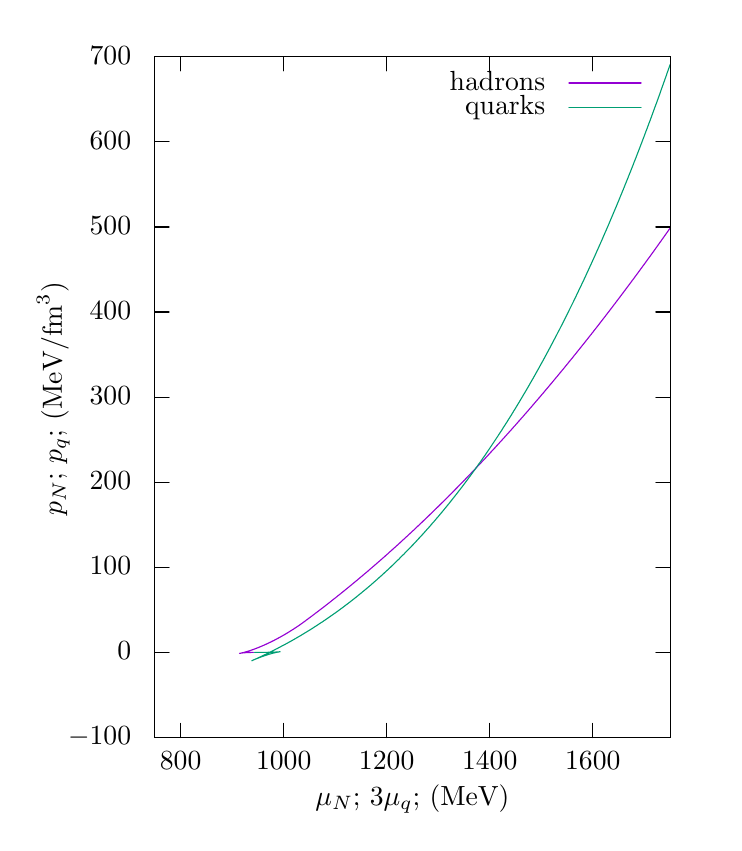
\begin{tikzpicture}[gnuplot]
%% generated with GNUPLOT 5.0p4 (Lua 5.2; terminal rev. 99, script rev. 100)
%% Thu Sep 29 16:33:17 2016
\path (0.000,0.000) rectangle (8.600,10.000);
\gpcolor{color=gp lt color border}
\gpsetlinetype{gp lt border}
\gpsetdashtype{gp dt solid}
\gpsetlinewidth{1.00}
\draw[gp path] (1.504,0.985)--(1.684,0.985);
\draw[gp path] (8.047,0.985)--(7.867,0.985);
\node[gp node right] at (1.320,0.985) {$-100$};
\draw[gp path] (1.504,2.066)--(1.684,2.066);
\draw[gp path] (8.047,2.066)--(7.867,2.066);
\node[gp node right] at (1.320,2.066) {$0$};
\draw[gp path] (1.504,3.147)--(1.684,3.147);
\draw[gp path] (8.047,3.147)--(7.867,3.147);
\node[gp node right] at (1.320,3.147) {$100$};
\draw[gp path] (1.504,4.227)--(1.684,4.227);
\draw[gp path] (8.047,4.227)--(7.867,4.227);
\node[gp node right] at (1.320,4.227) {$200$};
\draw[gp path] (1.504,5.308)--(1.684,5.308);
\draw[gp path] (8.047,5.308)--(7.867,5.308);
\node[gp node right] at (1.320,5.308) {$300$};
\draw[gp path] (1.504,6.389)--(1.684,6.389);
\draw[gp path] (8.047,6.389)--(7.867,6.389);
\node[gp node right] at (1.320,6.389) {$400$};
\draw[gp path] (1.504,7.469)--(1.684,7.469);
\draw[gp path] (8.047,7.469)--(7.867,7.469);
\node[gp node right] at (1.320,7.469) {$500$};
\draw[gp path] (1.504,8.550)--(1.684,8.550);
\draw[gp path] (8.047,8.550)--(7.867,8.550);
\node[gp node right] at (1.320,8.550) {$600$};
\draw[gp path] (1.504,9.631)--(1.684,9.631);
\draw[gp path] (8.047,9.631)--(7.867,9.631);
\node[gp node right] at (1.320,9.631) {$700$};
\draw[gp path] (1.831,0.985)--(1.831,1.165);
\draw[gp path] (1.831,9.631)--(1.831,9.451);
\node[gp node center] at (1.831,0.677) {$800$};
\draw[gp path] (3.140,0.985)--(3.140,1.165);
\draw[gp path] (3.140,9.631)--(3.140,9.451);
\node[gp node center] at (3.140,0.677) {$1000$};
\draw[gp path] (4.448,0.985)--(4.448,1.165);
\draw[gp path] (4.448,9.631)--(4.448,9.451);
\node[gp node center] at (4.448,0.677) {$1200$};
\draw[gp path] (5.757,0.985)--(5.757,1.165);
\draw[gp path] (5.757,9.631)--(5.757,9.451);
\node[gp node center] at (5.757,0.677) {$1400$};
\draw[gp path] (7.066,0.985)--(7.066,1.165);
\draw[gp path] (7.066,9.631)--(7.066,9.451);
\node[gp node center] at (7.066,0.677) {$1600$};
\draw[gp path] (1.504,9.631)--(1.504,0.985)--(8.047,0.985)--(8.047,9.631)--cycle;
\node[gp node center,rotate=-270] at (0.246,5.308) {$p_N$; $p_q$; ($\rm{MeV}/\rm{fm}^3$)};
\node[gp node center] at (4.775,0.215) {$\mu_N$; $3\mu_q$; (MeV)};
\node[gp node right] at (6.579,9.297) {hadrons};
\gpcolor{rgb color={0.580,0.000,0.827}}
\draw[gp path] (6.763,9.297)--(7.679,9.297);
\draw[gp path] (2.725,2.066)--(2.732,2.066)--(2.739,2.066)--(2.745,2.066)--(2.751,2.066)%
  --(2.757,2.066)--(2.725,2.066)--(2.731,2.066)--(2.737,2.066)--(2.743,2.066)--(2.748,2.066)%
  --(2.716,2.065)--(2.721,2.066)--(2.727,2.066)--(2.732,2.066)--(2.738,2.066)--(2.705,2.065)%
  --(2.711,2.065)--(2.716,2.065)--(2.722,2.066)--(2.727,2.066)--(2.733,2.066)--(2.700,2.065)%
  --(2.706,2.065)--(2.711,2.065)--(2.717,2.065)--(2.722,2.066)--(2.690,2.065)--(2.695,2.065)%
  --(2.700,2.065)--(2.706,2.065)--(2.711,2.065)--(2.679,2.064)--(2.684,2.064)--(2.690,2.065)%
  --(2.695,2.065)--(2.700,2.065)--(2.706,2.065)--(2.673,2.064)--(2.679,2.064)--(2.684,2.064)%
  --(2.690,2.065)--(2.695,2.065)--(2.663,2.063)--(2.668,2.063)--(2.674,2.064)--(2.679,2.064)%
  --(2.685,2.064)--(2.690,2.065)--(2.658,2.063)--(2.663,2.063)--(2.669,2.063)--(2.674,2.064)%
  --(2.680,2.064)--(2.648,2.062)--(2.653,2.063)--(2.659,2.063)--(2.664,2.063)--(2.670,2.064)%
  --(2.675,2.064)--(2.643,2.062)--(2.649,2.062)--(2.654,2.063)--(2.660,2.063)--(2.665,2.063)%
  --(2.634,2.061)--(2.639,2.061)--(2.645,2.062)--(2.650,2.062)--(2.656,2.063)--(2.661,2.063)%
  --(2.630,2.061)--(2.635,2.061)--(2.641,2.062)--(2.647,2.062)--(2.652,2.063)--(2.621,2.060)%
  --(2.626,2.060)--(2.632,2.061)--(2.638,2.061)--(2.643,2.062)--(2.649,2.062)--(2.617,2.059)%
  --(2.623,2.060)--(2.629,2.061)--(2.635,2.061)--(2.640,2.062)--(2.609,2.059)--(2.615,2.059)%
  --(2.620,2.060)--(2.626,2.060)--(2.632,2.061)--(2.638,2.061)--(2.606,2.058)--(2.612,2.059)%
  --(2.618,2.059)--(2.624,2.060)--(2.630,2.061)--(2.635,2.061)--(2.604,2.058)--(2.610,2.059)%
  --(2.616,2.059)--(2.622,2.060)--(2.628,2.061)--(2.597,2.057)--(2.602,2.058)--(2.608,2.058)%
  --(2.614,2.059)--(2.620,2.060)--(2.626,2.060)--(2.595,2.057)--(2.601,2.057)--(2.607,2.058)%
  --(2.613,2.059)--(2.619,2.060)--(2.588,2.056)--(2.594,2.056)--(2.600,2.057)--(2.606,2.058)%
  --(2.612,2.059)--(2.618,2.060)--(2.587,2.055)--(2.593,2.056)--(2.599,2.057)--(2.605,2.058)%
  --(2.611,2.059)--(2.618,2.060)--(2.587,2.055)--(2.593,2.056)--(2.599,2.057)--(2.605,2.058)%
  --(2.611,2.059)--(2.617,2.060)--(2.587,2.055)--(2.593,2.056)--(2.599,2.057)--(2.605,2.058)%
  --(2.612,2.059)--(2.581,2.054)--(2.588,2.055)--(2.594,2.056)--(2.600,2.057)--(2.606,2.058)%
  --(2.612,2.059)--(2.582,2.054)--(2.588,2.055)--(2.595,2.056)--(2.601,2.057)--(2.607,2.058)%
  --(2.613,2.059)--(2.583,2.054)--(2.590,2.055)--(2.596,2.057)--(2.602,2.058)--(2.608,2.059)%
  --(2.579,2.054)--(2.585,2.055)--(2.591,2.056)--(2.597,2.057)--(2.604,2.058)--(2.610,2.059)%
  --(2.580,2.054)--(2.587,2.055)--(2.593,2.056)--(2.600,2.057)--(2.606,2.058)--(2.612,2.060)%
  --(2.583,2.054)--(2.589,2.055)--(2.596,2.056)--(2.602,2.058)--(2.608,2.059)--(2.615,2.060)%
  --(2.585,2.054)--(2.592,2.056)--(2.598,2.057)--(2.605,2.058)--(2.611,2.059)--(2.618,2.061)%
  --(2.588,2.055)--(2.595,2.056)--(2.601,2.058)--(2.608,2.059)--(2.614,2.060)--(2.585,2.054)%
  --(2.592,2.056)--(2.598,2.057)--(2.605,2.058)--(2.611,2.060)--(2.618,2.061)--(2.589,2.055)%
  --(2.596,2.056)--(2.602,2.058)--(2.609,2.059)--(2.615,2.061)--(2.622,2.062)--(2.593,2.056)%
  --(2.600,2.057)--(2.606,2.059)--(2.613,2.060)--(2.620,2.062)--(2.626,2.063)--(2.598,2.057)%
  --(2.604,2.058)--(2.611,2.060)--(2.618,2.061)--(2.624,2.063)--(2.596,2.056)--(2.603,2.058)%
  --(2.609,2.059)--(2.616,2.061)--(2.623,2.062)--(2.629,2.064)--(2.601,2.057)--(2.608,2.059)%
  --(2.614,2.060)--(2.621,2.062)--(2.628,2.064)--(2.635,2.065)--(2.607,2.058)--(2.613,2.060)%
  --(2.620,2.062)--(2.627,2.063)--(2.634,2.065)--(2.640,2.067)--(2.612,2.060)--(2.619,2.062)%
  --(2.626,2.063)--(2.633,2.065)--(2.640,2.067)--(2.647,2.068)--(2.619,2.061)--(2.626,2.063)%
  --(2.632,2.065)--(2.639,2.067)--(2.646,2.068)--(2.619,2.061)--(2.625,2.063)--(2.632,2.065)%
  --(2.639,2.067)--(2.646,2.068)--(2.653,2.070)--(2.625,2.063)--(2.632,2.065)--(2.639,2.067)%
  --(2.646,2.069)--(2.653,2.070)--(2.660,2.072)--(2.633,2.065)--(2.640,2.067)--(2.647,2.069)%
  --(2.654,2.071)--(2.661,2.073)--(2.668,2.075)--(2.640,2.067)--(2.648,2.069)--(2.655,2.071)%
  --(2.662,2.073)--(2.669,2.075)--(2.676,2.077)--(2.649,2.069)--(2.656,2.071)--(2.663,2.073)%
  --(2.670,2.075)--(2.677,2.077)--(2.650,2.069)--(2.657,2.071)--(2.664,2.074)--(2.671,2.076)%
  --(2.678,2.078)--(2.685,2.080)--(2.659,2.072)--(2.666,2.074)--(2.673,2.076)--(2.680,2.078)%
  --(2.687,2.080)--(2.694,2.083)--(2.668,2.074)--(2.675,2.077)--(2.682,2.079)--(2.689,2.081)%
  --(2.696,2.083)--(2.703,2.086)--(2.677,2.077)--(2.684,2.080)--(2.691,2.082)--(2.699,2.084)%
  --(2.706,2.086)--(2.679,2.078)--(2.687,2.080)--(2.694,2.083)--(2.701,2.085)--(2.708,2.087)%
  --(2.716,2.090)--(2.689,2.081)--(2.697,2.084)--(2.704,2.086)--(2.711,2.088)--(2.719,2.091)%
  --(2.726,2.093)--(2.700,2.084)--(2.707,2.087)--(2.714,2.089)--(2.722,2.092)--(2.729,2.094)%
  --(2.736,2.097)--(2.710,2.088)--(2.718,2.090)--(2.725,2.093)--(2.732,2.095)--(2.740,2.098)%
  --(2.714,2.089)--(2.722,2.092)--(2.729,2.094)--(2.736,2.097)--(2.744,2.099)--(2.751,2.102)%
  --(2.725,2.093)--(2.733,2.096)--(2.740,2.098)--(2.748,2.101)--(2.755,2.103)--(2.762,2.106)%
  --(2.737,2.097)--(2.745,2.100)--(2.752,2.102)--(2.759,2.105)--(2.767,2.108)--(2.742,2.099)%
  --(2.749,2.101)--(2.757,2.104)--(2.764,2.107)--(2.771,2.109)--(2.779,2.112)--(2.754,2.103)%
  --(2.761,2.106)--(2.769,2.109)--(2.776,2.111)--(2.784,2.114)--(2.767,2.108)--(2.775,2.111)%
  --(2.782,2.113)--(2.773,2.110)--(2.781,2.113)--(2.788,2.116)--(2.780,2.113)--(2.787,2.116)%
  --(2.795,2.118)--(2.786,2.115)--(2.794,2.118)--(2.801,2.121)--(2.793,2.118)--(2.801,2.121)%
  --(2.792,2.117)--(2.800,2.120)--(2.807,2.123)--(2.799,2.120)--(2.806,2.123)--(2.814,2.126)%
  --(2.806,2.123)--(2.813,2.126)--(2.821,2.129)--(2.813,2.125)--(2.820,2.128)--(2.812,2.125)%
  --(2.820,2.128)--(2.827,2.131)--(2.819,2.128)--(2.827,2.131)--(2.834,2.134)--(2.826,2.131)%
  --(2.834,2.134)--(2.841,2.137)--(2.833,2.134)--(2.841,2.137)--(2.833,2.134)--(2.841,2.137)%
  --(2.848,2.140)--(2.840,2.137)--(2.848,2.140)--(2.856,2.143)--(2.848,2.140)--(2.855,2.143)%
  --(2.848,2.140)--(2.855,2.143)--(2.863,2.146)--(2.855,2.143)--(2.863,2.146)--(2.871,2.149)%
  --(2.863,2.146)--(2.870,2.149)--(2.863,2.146)--(2.870,2.149)--(2.878,2.153)--(2.871,2.149)%
  --(2.878,2.153)--(2.886,2.156)--(2.878,2.153)--(2.886,2.156)--(2.879,2.153)--(2.886,2.156)%
  --(2.894,2.160)--(2.887,2.156)--(2.894,2.160)--(2.902,2.163)--(2.895,2.160)--(2.902,2.163)%
  --(2.895,2.160)--(2.903,2.164)--(2.910,2.167)--(2.903,2.164)--(2.911,2.167)--(2.919,2.171)%
  --(2.911,2.168)--(2.919,2.171)--(2.912,2.168)--(2.920,2.171)--(2.927,2.175)--(2.920,2.172)%
  --(2.928,2.175)--(2.921,2.172)--(2.929,2.176)--(2.937,2.179)--(2.929,2.176)--(2.937,2.180)%
  --(2.945,2.183)--(2.938,2.180)--(2.946,2.184)--(2.939,2.180)--(2.947,2.184)--(2.955,2.188)%
  --(2.948,2.184)--(2.955,2.188)--(2.949,2.185)--(2.956,2.189)--(2.964,2.192)--(2.957,2.189)%
  --(2.965,2.193)--(2.959,2.190)--(2.966,2.193)--(2.974,2.197)--(2.968,2.194)--(2.975,2.198)%
  --(2.969,2.195)--(2.977,2.198)--(2.984,2.202)--(2.978,2.199)--(2.986,2.203)--(2.979,2.200)%
  --(2.987,2.204)--(2.995,2.208)--(2.988,2.204)--(2.996,2.208)--(2.990,2.205)--(2.998,2.209)%
  --(3.006,2.213)--(2.999,2.210)--(3.007,2.214)--(3.001,2.210)--(3.009,2.214)--(3.017,2.218)%
  --(3.010,2.215)--(3.018,2.219)--(3.012,2.216)--(3.020,2.220)--(3.014,2.217)--(3.022,2.221)%
  --(3.030,2.225)--(3.024,2.222)--(3.031,2.226)--(3.025,2.223)--(3.033,2.227)--(3.041,2.231)%
  --(3.035,2.228)--(3.043,2.232)--(3.037,2.229)--(3.045,2.233)--(3.039,2.230)--(3.047,2.234)%
  --(3.055,2.239)--(3.049,2.236)--(3.057,2.240)--(3.052,2.237)--(3.060,2.241)--(3.054,2.238)%
  --(3.062,2.242)--(3.070,2.246)--(3.064,2.243)--(3.072,2.248)--(3.066,2.245)--(3.074,2.249)%
  --(3.069,2.246)--(3.077,2.250)--(3.085,2.255)--(3.079,2.252)--(3.087,2.256)--(3.082,2.253)%
  --(3.090,2.257)--(3.084,2.254)--(3.092,2.259)--(3.100,2.263)--(3.095,2.260)--(3.103,2.265)%
  --(3.098,2.262)--(3.106,2.266)--(3.101,2.263)--(3.109,2.268)--(3.103,2.265)--(3.111,2.269)%
  --(3.106,2.267)--(3.114,2.271)--(3.122,2.275)--(3.117,2.273)--(3.125,2.277)--(3.120,2.274)%
  --(3.128,2.279)--(3.124,2.276)--(3.132,2.281)--(3.127,2.278)--(3.135,2.283)--(3.130,2.280)%
  --(3.138,2.284)--(3.133,2.282)--(3.141,2.286)--(3.149,2.291)--(3.145,2.288)--(3.153,2.293)%
  --(3.148,2.290)--(3.156,2.295)--(3.152,2.292)--(3.160,2.297)--(3.155,2.294)--(3.163,2.299)%
  --(3.159,2.297)--(3.167,2.301)--(3.163,2.299)--(3.171,2.303)--(3.166,2.301)--(3.174,2.306)%
  --(3.170,2.303)--(3.178,2.308)--(3.174,2.306)--(3.182,2.310)--(3.178,2.308)--(3.186,2.313)%
  --(3.182,2.310)--(3.190,2.315)--(3.186,2.313)--(3.194,2.318)--(3.190,2.315)--(3.198,2.320)%
  --(3.195,2.318)--(3.203,2.323)--(3.199,2.321)--(3.207,2.325)--(3.203,2.323)--(3.211,2.328)%
  --(3.208,2.326)--(3.216,2.331)--(3.212,2.329)--(3.220,2.334)--(3.217,2.332)--(3.225,2.337)%
  --(3.222,2.335)--(3.218,2.333)--(3.226,2.337)--(3.223,2.336)--(3.231,2.340)--(3.228,2.339)%
  --(3.236,2.344)--(3.233,2.342)--(3.241,2.347)--(3.238,2.345)--(3.246,2.350)--(3.243,2.348)%
  --(3.246,2.350)--(3.248,2.351)--(3.251,2.353)--(3.254,2.355)--(3.256,2.356)--(3.254,2.355)%
  --(3.257,2.357)--(3.259,2.358)--(3.262,2.360)--(3.265,2.362)--(3.268,2.364)--(3.266,2.362)%
  --(3.269,2.364)--(3.271,2.366)--(3.274,2.368)--(3.272,2.367)--(3.275,2.369)--(3.278,2.371)%
  --(3.281,2.373)--(3.284,2.375)--(3.283,2.373)--(3.286,2.375)--(3.289,2.378)--(3.287,2.376)%
  --(3.290,2.379)--(3.294,2.381)--(3.297,2.383)--(3.295,2.382)--(3.299,2.384)--(3.302,2.386)%
  --(3.301,2.385)--(3.304,2.388)--(3.308,2.390)--(3.306,2.389)--(3.310,2.392)--(3.309,2.391)%
  --(3.313,2.393)--(3.316,2.396)--(3.315,2.395)--(3.319,2.398)--(3.318,2.397)--(3.322,2.400)%
  --(3.321,2.399)--(3.325,2.402)--(3.329,2.404)--(3.332,2.407)--(3.336,2.410)--(3.337,2.410)%
  --(3.341,2.413)--(3.346,2.416)--(3.347,2.417)--(3.348,2.418)--(3.352,2.421)--(3.353,2.421)%
  --(3.354,2.422)--(3.355,2.423)--(3.356,2.424)--(3.358,2.425)--(3.359,2.426)--(3.361,2.427)%
  --(3.362,2.428)--(3.365,2.430)--(3.367,2.431)--(3.369,2.433)--(3.370,2.433)--(3.373,2.435)%
  --(3.374,2.436)--(3.375,2.437)--(3.377,2.438)--(3.378,2.439)--(3.380,2.441)--(3.381,2.441)%
  --(3.383,2.443)--(3.385,2.444)--(3.387,2.446)--(3.388,2.447)--(3.390,2.448)--(3.391,2.449)%
  --(3.393,2.450)--(3.394,2.451)--(3.396,2.452)--(3.397,2.453)--(3.398,2.454)--(3.400,2.455)%
  --(3.406,2.459)--(3.414,2.465)--(3.421,2.471)--(3.429,2.477)--(3.437,2.482)--(3.445,2.488)%
  --(3.452,2.494)--(3.460,2.500)--(3.468,2.505)--(3.476,2.511)--(3.483,2.517)--(3.491,2.523)%
  --(3.499,2.529)--(3.507,2.534)--(3.514,2.540)--(3.522,2.546)--(3.530,2.552)--(3.537,2.558)%
  --(3.545,2.564)--(3.553,2.570)--(3.561,2.575)--(3.568,2.581)--(3.576,2.587)--(3.584,2.593)%
  --(3.592,2.599)--(3.599,2.605)--(3.607,2.611)--(3.615,2.617)--(3.622,2.623)--(3.630,2.629)%
  --(3.638,2.634)--(3.646,2.640)--(3.653,2.646)--(3.661,2.652)--(3.669,2.658)--(3.676,2.664)%
  --(3.684,2.670)--(3.692,2.676)--(3.699,2.682)--(3.707,2.688)--(3.715,2.694)--(3.723,2.700)%
  --(3.730,2.706)--(3.738,2.712)--(3.746,2.718)--(3.753,2.725)--(3.761,2.731)--(3.769,2.737)%
  --(3.776,2.743)--(3.784,2.749)--(3.792,2.755)--(3.800,2.761)--(3.807,2.767)--(3.815,2.773)%
  --(3.823,2.779)--(3.830,2.786)--(3.838,2.792)--(3.846,2.798)--(3.853,2.804)--(3.861,2.810)%
  --(3.869,2.816)--(3.876,2.822)--(3.884,2.829)--(3.892,2.835)--(3.899,2.841)--(3.907,2.847)%
  --(3.915,2.854)--(3.922,2.860)--(3.930,2.866)--(3.938,2.872)--(3.945,2.878)--(3.953,2.885)%
  --(3.961,2.891)--(3.968,2.897)--(3.976,2.904)--(3.984,2.910)--(3.991,2.916)--(3.999,2.922)%
  --(4.007,2.929)--(4.014,2.935)--(4.022,2.941)--(4.030,2.948)--(4.037,2.954)--(4.045,2.960)%
  --(4.053,2.967)--(4.060,2.973)--(4.068,2.979)--(4.076,2.986)--(4.083,2.992)--(4.091,2.999)%
  --(4.099,3.005)--(4.106,3.011)--(4.114,3.018)--(4.122,3.024)--(4.129,3.031)--(4.137,3.037)%
  --(4.144,3.044)--(4.152,3.050)--(4.160,3.056)--(4.167,3.063)--(4.175,3.069)--(4.183,3.076)%
  --(4.190,3.082)--(4.198,3.089)--(4.206,3.095)--(4.213,3.102)--(4.221,3.108)--(4.228,3.115)%
  --(4.236,3.122)--(4.244,3.128)--(4.251,3.135)--(4.259,3.141)--(4.267,3.148)--(4.274,3.154)%
  --(4.282,3.161)--(4.289,3.167)--(4.297,3.174)--(4.305,3.181)--(4.312,3.187)--(4.320,3.194)%
  --(4.328,3.201)--(4.335,3.207)--(4.343,3.214)--(4.350,3.220)--(4.358,3.227)--(4.366,3.234)%
  --(4.373,3.240)--(4.381,3.247)--(4.389,3.254)--(4.396,3.261)--(4.404,3.267)--(4.411,3.274)%
  --(4.419,3.281)--(4.427,3.287)--(4.434,3.294)--(4.442,3.301)--(4.449,3.308)--(4.457,3.314)%
  --(4.465,3.321)--(4.472,3.328)--(4.480,3.335)--(4.487,3.342)--(4.495,3.348)--(4.503,3.355)%
  --(4.510,3.362)--(4.518,3.369)--(4.525,3.376)--(4.533,3.382)--(4.541,3.389)--(4.548,3.396)%
  --(4.556,3.403)--(4.563,3.410)--(4.571,3.417)--(4.579,3.424)--(4.586,3.430)--(4.594,3.437)%
  --(4.601,3.444)--(4.609,3.451)--(4.617,3.458)--(4.624,3.465)--(4.632,3.472)--(4.639,3.479)%
  --(4.647,3.486)--(4.654,3.493)--(4.662,3.500)--(4.670,3.507)--(4.677,3.514)--(4.685,3.521)%
  --(4.692,3.528)--(4.700,3.535)--(4.708,3.542)--(4.715,3.549)--(4.723,3.556)--(4.730,3.563)%
  --(4.738,3.570)--(4.745,3.577)--(4.753,3.584)--(4.761,3.591)--(4.768,3.598)--(4.776,3.605)%
  --(4.783,3.612)--(4.791,3.619)--(4.798,3.626)--(4.806,3.633)--(4.814,3.641)--(4.821,3.648)%
  --(4.829,3.655)--(4.836,3.662)--(4.844,3.669)--(4.851,3.676)--(4.859,3.683)--(4.866,3.691)%
  --(4.874,3.698)--(4.882,3.705)--(4.889,3.712)--(4.897,3.719)--(4.904,3.727)--(4.912,3.734)%
  --(4.919,3.741)--(4.927,3.748)--(4.934,3.755)--(4.942,3.763)--(4.950,3.770)--(4.957,3.777)%
  --(4.965,3.784)--(4.972,3.792)--(4.980,3.799)--(4.987,3.806)--(4.995,3.814)--(5.002,3.821)%
  --(5.010,3.828)--(5.017,3.835)--(5.025,3.843)--(5.033,3.850)--(5.040,3.857)--(5.048,3.865)%
  --(5.055,3.872)--(5.063,3.880)--(5.070,3.887)--(5.078,3.894)--(5.085,3.902)--(5.093,3.909)%
  --(5.100,3.916)--(5.108,3.924)--(5.116,3.931)--(5.123,3.939)--(5.131,3.946)--(5.138,3.954)%
  --(5.146,3.961)--(5.153,3.969)--(5.161,3.976)--(5.168,3.983)--(5.176,3.991)--(5.183,3.998)%
  --(5.191,4.006)--(5.198,4.013)--(5.206,4.021)--(5.213,4.028)--(5.221,4.036)--(5.228,4.043)%
  --(5.236,4.051)--(5.243,4.059)--(5.251,4.066)--(5.259,4.074)--(5.266,4.081)--(5.274,4.089)%
  --(5.281,4.096)--(5.289,4.104)--(5.296,4.112)--(5.304,4.119)--(5.311,4.127)--(5.319,4.134)%
  --(5.326,4.142)--(5.334,4.150)--(5.341,4.157)--(5.349,4.165)--(5.356,4.173)--(5.364,4.180)%
  --(5.371,4.188)--(5.379,4.196)--(5.386,4.203)--(5.394,4.211)--(5.401,4.219)--(5.409,4.226)%
  --(5.416,4.234)--(5.424,4.242)--(5.431,4.250)--(5.439,4.257)--(5.446,4.265)--(5.454,4.273)%
  --(5.461,4.281)--(5.469,4.288)--(5.476,4.296)--(5.484,4.304)--(5.491,4.312)--(5.499,4.320)%
  --(5.506,4.327)--(5.514,4.335)--(5.521,4.343)--(5.529,4.351)--(5.536,4.359)--(5.544,4.367)%
  --(5.551,4.374)--(5.559,4.382)--(5.566,4.390)--(5.574,4.398)--(5.581,4.406)--(5.589,4.414)%
  --(5.596,4.422)--(5.604,4.430)--(5.611,4.438)--(5.619,4.445)--(5.626,4.453)--(5.634,4.461)%
  --(5.641,4.469)--(5.649,4.477)--(5.656,4.485)--(5.664,4.493)--(5.671,4.501)--(5.679,4.509)%
  --(5.686,4.517)--(5.694,4.525)--(5.701,4.533)--(5.709,4.541)--(5.716,4.549)--(5.724,4.557)%
  --(5.731,4.565)--(5.738,4.573)--(5.746,4.581)--(5.753,4.589)--(5.761,4.597)--(5.768,4.606)%
  --(5.776,4.614)--(5.783,4.622)--(5.791,4.630)--(5.798,4.638)--(5.806,4.646)--(5.813,4.654)%
  --(5.821,4.662)--(5.828,4.670)--(5.836,4.679)--(5.843,4.687)--(5.851,4.695)--(5.858,4.703)%
  --(5.865,4.711)--(5.873,4.719)--(5.880,4.728)--(5.888,4.736)--(5.895,4.744)--(5.903,4.752)%
  --(5.910,4.760)--(5.918,4.769)--(5.925,4.777)--(5.933,4.785)--(5.940,4.793)--(5.948,4.802)%
  --(5.955,4.810)--(5.963,4.818)--(5.970,4.826)--(5.977,4.835)--(5.985,4.843)--(5.992,4.851)%
  --(6.000,4.860)--(6.007,4.868)--(6.015,4.876)--(6.022,4.885)--(6.030,4.893)--(6.037,4.901)%
  --(6.045,4.910)--(6.052,4.918)--(6.059,4.926)--(6.067,4.935)--(6.074,4.943)--(6.082,4.951)%
  --(6.089,4.960)--(6.097,4.968)--(6.104,4.977)--(6.112,4.985)--(6.119,4.994)--(6.126,5.002)%
  --(6.134,5.010)--(6.141,5.019)--(6.149,5.027)--(6.156,5.036)--(6.164,5.044)--(6.171,5.053)%
  --(6.179,5.061)--(6.186,5.070)--(6.193,5.078)--(6.201,5.087)--(6.208,5.095)--(6.216,5.104)%
  --(6.223,5.112)--(6.231,5.121)--(6.238,5.129)--(6.246,5.138)--(6.253,5.147)--(6.260,5.155)%
  --(6.268,5.164)--(6.275,5.172)--(6.283,5.181)--(6.290,5.189)--(6.298,5.198)--(6.305,5.207)%
  --(6.312,5.215)--(6.320,5.224)--(6.327,5.233)--(6.335,5.241)--(6.342,5.250)--(6.350,5.259)%
  --(6.357,5.267)--(6.364,5.276)--(6.372,5.285)--(6.379,5.293)--(6.387,5.302)--(6.394,5.311)%
  --(6.402,5.319)--(6.409,5.328)--(6.416,5.337)--(6.424,5.346)--(6.431,5.354)--(6.439,5.363)%
  --(6.446,5.372)--(6.454,5.381)--(6.461,5.389)--(6.468,5.398)--(6.476,5.407)--(6.483,5.416)%
  --(6.491,5.425)--(6.498,5.433)--(6.505,5.442)--(6.513,5.451)--(6.520,5.460)--(6.528,5.469)%
  --(6.535,5.478)--(6.543,5.486)--(6.550,5.495)--(6.557,5.504)--(6.565,5.513)--(6.572,5.522)%
  --(6.580,5.531)--(6.587,5.540)--(6.594,5.549)--(6.602,5.558)--(6.609,5.566)--(6.617,5.575)%
  --(6.624,5.584)--(6.631,5.593)--(6.639,5.602)--(6.646,5.611)--(6.654,5.620)--(6.661,5.629)%
  --(6.669,5.638)--(6.676,5.647)--(6.683,5.656)--(6.691,5.665)--(6.698,5.674)--(6.706,5.683)%
  --(6.713,5.692)--(6.720,5.701)--(6.728,5.710)--(6.735,5.719)--(6.743,5.728)--(6.750,5.737)%
  --(6.757,5.747)--(6.765,5.756)--(6.772,5.765)--(6.780,5.774)--(6.787,5.783)--(6.794,5.792)%
  --(6.802,5.801)--(6.809,5.810)--(6.817,5.819)--(6.824,5.829)--(6.831,5.838)--(6.839,5.847)%
  --(6.846,5.856)--(6.853,5.865)--(6.861,5.874)--(6.868,5.884)--(6.876,5.893)--(6.883,5.902)%
  --(6.890,5.911)--(6.898,5.920)--(6.905,5.930)--(6.913,5.939)--(6.920,5.948)--(6.927,5.957)%
  --(6.935,5.967)--(6.942,5.976)--(6.950,5.985)--(6.957,5.994)--(6.964,6.004)--(6.972,6.013)%
  --(6.979,6.022)--(6.986,6.032)--(6.994,6.041)--(7.001,6.050)--(7.009,6.060)--(7.016,6.069)%
  --(7.023,6.078)--(7.031,6.088)--(7.038,6.097)--(7.046,6.106)--(7.053,6.116)--(7.060,6.125)%
  --(7.068,6.134)--(7.075,6.144)--(7.082,6.153)--(7.090,6.163)--(7.097,6.172)--(7.105,6.182)%
  --(7.112,6.191)--(7.119,6.200)--(7.127,6.210)--(7.134,6.219)--(7.141,6.229)--(7.149,6.238)%
  --(7.156,6.248)--(7.164,6.257)--(7.171,6.267)--(7.178,6.276)--(7.186,6.286)--(7.193,6.295)%
  --(7.200,6.305)--(7.208,6.314)--(7.215,6.324)--(7.223,6.333)--(7.230,6.343)--(7.237,6.353)%
  --(7.245,6.362)--(7.252,6.372)--(7.259,6.381)--(7.267,6.391)--(7.274,6.400)--(7.281,6.410)%
  --(7.289,6.420)--(7.296,6.429)--(7.304,6.439)--(7.311,6.449)--(7.318,6.458)--(7.326,6.468)%
  --(7.333,6.478)--(7.340,6.487)--(7.348,6.497)--(7.355,6.507)--(7.362,6.516)--(7.370,6.526)%
  --(7.377,6.536)--(7.384,6.545)--(7.392,6.555)--(7.399,6.565)--(7.407,6.575)--(7.414,6.584)%
  --(7.421,6.594)--(7.429,6.604)--(7.436,6.614)--(7.443,6.623)--(7.451,6.633)--(7.458,6.643)%
  --(7.465,6.653)--(7.473,6.663)--(7.480,6.672)--(7.487,6.682)--(7.495,6.692)--(7.502,6.702)%
  --(7.510,6.712)--(7.517,6.722)--(7.524,6.731)--(7.532,6.741)--(7.539,6.751)--(7.546,6.761)%
  --(7.554,6.771)--(7.561,6.781)--(7.568,6.791)--(7.576,6.801)--(7.583,6.810)--(7.590,6.820)%
  --(7.598,6.830)--(7.605,6.840)--(7.612,6.850)--(7.620,6.860)--(7.627,6.870)--(7.634,6.880)%
  --(7.642,6.890)--(7.649,6.900)--(7.656,6.910)--(7.664,6.920)--(7.671,6.930)--(7.678,6.940)%
  --(7.686,6.950)--(7.693,6.960)--(7.700,6.970)--(7.708,6.980)--(7.715,6.990)--(7.723,7.000)%
  --(7.730,7.010)--(7.737,7.020)--(7.745,7.031)--(7.752,7.041)--(7.759,7.051)--(7.767,7.061)%
  --(7.774,7.071)--(7.781,7.081)--(7.789,7.091)--(7.796,7.101)--(7.803,7.111)--(7.811,7.122)%
  --(7.818,7.132)--(7.825,7.142)--(7.833,7.152)--(7.840,7.162)--(7.847,7.172)--(7.855,7.183)%
  --(7.862,7.193)--(7.869,7.203)--(7.877,7.213)--(7.884,7.224)--(7.891,7.234)--(7.898,7.244)%
  --(7.906,7.254)--(7.913,7.264)--(7.920,7.275)--(7.928,7.285)--(7.935,7.295)--(7.942,7.306)%
  --(7.950,7.316)--(7.957,7.326)--(7.964,7.336)--(7.972,7.347)--(7.979,7.357)--(7.986,7.367)%
  --(7.994,7.378)--(8.001,7.388)--(8.008,7.398)--(8.016,7.409)--(8.023,7.419)--(8.030,7.430)%
  --(8.038,7.440)--(8.045,7.450)--(8.047,7.453);
\gpcolor{color=gp lt color border}
\node[gp node right] at (6.579,8.989) {quarks};
\gpcolor{rgb color={0.000,0.620,0.451}}
\draw[gp path] (6.763,8.989)--(7.679,8.989);
\draw[gp path] (2.770,2.066)--(2.819,2.066)--(2.852,2.066)--(2.879,2.066)--(2.901,2.067)%
  --(2.920,2.067)--(2.936,2.067)--(2.951,2.068)--(2.964,2.068)--(2.976,2.068)--(2.987,2.068)%
  --(2.997,2.069)--(3.006,2.069)--(3.014,2.069)--(3.022,2.070)--(3.029,2.070)--(3.035,2.070)%
  --(3.041,2.071)--(3.047,2.071)--(3.052,2.071)--(3.056,2.071)--(3.061,2.072)--(3.065,2.072)%
  --(3.068,2.072)--(3.072,2.073)--(3.075,2.073)--(3.077,2.073)--(3.080,2.073)--(3.082,2.073)%
  --(3.084,2.074)--(3.086,2.074)--(3.088,2.074)--(3.089,2.074)--(3.090,2.074)--(3.092,2.074)%
  --(3.093,2.074)--(3.094,2.074)--(3.095,2.075)--(3.094,2.074)--(3.093,2.074)--(3.092,2.074)%
  --(3.091,2.074)--(3.090,2.074)--(3.089,2.074)--(3.088,2.074)--(3.086,2.073)--(3.085,2.073)%
  --(3.084,2.073)--(3.082,2.073)--(3.080,2.072)--(3.079,2.072)--(3.077,2.072)--(3.075,2.071)%
  --(3.073,2.071)--(3.071,2.071)--(3.069,2.070)--(3.067,2.070)--(3.065,2.070)--(3.063,2.069)%
  --(3.061,2.069)--(3.058,2.068)--(3.056,2.068)--(3.053,2.067)--(3.051,2.067)--(3.048,2.066)%
  --(3.046,2.066)--(3.043,2.065)--(3.040,2.064)--(3.037,2.064)--(3.034,2.063)--(3.031,2.062)%
  --(3.029,2.062)--(3.026,2.061)--(3.022,2.060)--(3.019,2.060)--(3.016,2.059)--(3.013,2.058)%
  --(3.010,2.057)--(3.007,2.056)--(3.003,2.056)--(3.000,2.055)--(2.997,2.054)--(2.993,2.053)%
  --(2.990,2.052)--(2.986,2.051)--(2.983,2.050)--(2.979,2.049)--(2.975,2.048)--(2.972,2.047)%
  --(2.968,2.046)--(2.965,2.045)--(2.961,2.044)--(2.957,2.043)--(2.953,2.042)--(2.949,2.040)%
  --(2.945,2.039)--(2.942,2.038)--(2.938,2.037)--(2.934,2.036)--(2.930,2.034)--(2.926,2.033)%
  --(2.922,2.032)--(2.918,2.030)--(2.913,2.029)--(2.909,2.028)--(2.905,2.026)--(2.901,2.025)%
  --(2.897,2.023)--(2.892,2.022)--(2.888,2.021)--(2.884,2.019)--(2.880,2.018)--(2.875,2.016)%
  --(2.871,2.014)--(2.866,2.013)--(2.862,2.011)--(2.858,2.010)--(2.853,2.008)--(2.849,2.006)%
  --(2.844,2.005)--(2.840,2.003)--(2.835,2.001)--(2.831,2.000)--(2.826,1.998)--(2.821,1.996)%
  --(2.817,1.994)--(2.812,1.992)--(2.807,1.990)--(2.803,1.989)--(2.798,1.987)--(2.793,1.985)%
  --(2.788,1.983)--(2.784,1.981)--(2.779,1.979)--(2.774,1.977)--(2.769,1.975)--(2.764,1.973)%
  --(2.760,1.971)--(2.755,1.969)--(2.750,1.966)--(2.745,1.964)--(2.740,1.962)--(2.735,1.960)%
  --(2.743,1.964)--(2.757,1.970)--(2.770,1.976)--(2.783,1.982)--(2.797,1.988)--(2.810,1.994)%
  --(2.823,2.000)--(2.836,2.006)--(2.849,2.012)--(2.862,2.018)--(2.875,2.024)--(2.888,2.031)%
  --(2.901,2.037)--(2.914,2.043)--(2.927,2.049)--(2.939,2.055)--(2.952,2.062)--(2.965,2.068)%
  --(2.977,2.074)--(2.990,2.080)--(3.002,2.087)--(3.015,2.093)--(3.027,2.099)--(3.039,2.106)%
  --(3.052,2.112)--(3.064,2.118)--(3.076,2.125)--(3.088,2.131)--(3.100,2.137)--(3.112,2.144)%
  --(3.124,2.150)--(3.136,2.156)--(3.148,2.163)--(3.160,2.169)--(3.172,2.176)--(3.184,2.182)%
  --(3.196,2.189)--(3.207,2.195)--(3.219,2.202)--(3.231,2.208)--(3.242,2.215)--(3.254,2.221)%
  --(3.265,2.228)--(3.277,2.234)--(3.288,2.241)--(3.299,2.247)--(3.311,2.254)--(3.322,2.261)%
  --(3.333,2.267)--(3.345,2.274)--(3.356,2.280)--(3.367,2.287)--(3.378,2.294)--(3.389,2.300)%
  --(3.400,2.307)--(3.411,2.314)--(3.422,2.320)--(3.433,2.327)--(3.444,2.334)--(3.455,2.340)%
  --(3.466,2.347)--(3.477,2.354)--(3.487,2.361)--(3.498,2.367)--(3.509,2.374)--(3.519,2.381)%
  --(3.530,2.388)--(3.541,2.395)--(3.551,2.401)--(3.562,2.408)--(3.572,2.415)--(3.583,2.422)%
  --(3.593,2.429)--(3.604,2.436)--(3.614,2.443)--(3.624,2.449)--(3.635,2.456)--(3.645,2.463)%
  --(3.655,2.470)--(3.666,2.477)--(3.676,2.484)--(3.686,2.491)--(3.696,2.498)--(3.706,2.505)%
  --(3.716,2.512)--(3.726,2.519)--(3.736,2.526)--(3.746,2.533)--(3.756,2.540)--(3.766,2.547)%
  --(3.776,2.554)--(3.786,2.561)--(3.796,2.568)--(3.806,2.575)--(3.816,2.582)--(3.825,2.589)%
  --(3.835,2.596)--(3.845,2.603)--(3.855,2.610)--(3.864,2.618)--(3.874,2.625)--(3.884,2.632)%
  --(3.893,2.639)--(3.903,2.646)--(3.912,2.653)--(3.922,2.661)--(3.931,2.668)--(3.941,2.675)%
  --(3.950,2.682)--(3.960,2.689)--(3.969,2.697)--(3.979,2.704)--(3.988,2.711)--(3.997,2.718)%
  --(4.007,2.726)--(4.016,2.733)--(4.025,2.740)--(4.034,2.747)--(4.044,2.755)--(4.053,2.762)%
  --(4.062,2.769)--(4.071,2.777)--(4.080,2.784)--(4.089,2.791)--(4.098,2.799)--(4.107,2.806)%
  --(4.116,2.813)--(4.126,2.821)--(4.135,2.828)--(4.143,2.836)--(4.152,2.843)--(4.161,2.850)%
  --(4.170,2.858)--(4.179,2.865)--(4.188,2.873)--(4.197,2.880)--(4.206,2.888)--(4.215,2.895)%
  --(4.223,2.902)--(4.232,2.910)--(4.241,2.917)--(4.250,2.925)--(4.258,2.932)--(4.267,2.940)%
  --(4.276,2.948)--(4.284,2.955)--(4.293,2.963)--(4.302,2.970)--(4.310,2.978)--(4.319,2.985)%
  --(4.327,2.993)--(4.336,3.000)--(4.344,3.008)--(4.353,3.016)--(4.361,3.023)--(4.370,3.031)%
  --(4.378,3.038)--(4.387,3.046)--(4.395,3.054)--(4.403,3.061)--(4.412,3.069)--(4.420,3.077)%
  --(4.428,3.084)--(4.437,3.092)--(4.445,3.100)--(4.453,3.107)--(4.462,3.115)--(4.470,3.123)%
  --(4.478,3.131)--(4.486,3.138)--(4.495,3.146)--(4.503,3.154)--(4.511,3.162)--(4.519,3.169)%
  --(4.527,3.177)--(4.535,3.185)--(4.543,3.193)--(4.551,3.200)--(4.559,3.208)--(4.568,3.216)%
  --(4.576,3.224)--(4.584,3.232)--(4.592,3.240)--(4.600,3.247)--(4.608,3.255)--(4.615,3.263)%
  --(4.623,3.271)--(4.631,3.279)--(4.639,3.287)--(4.647,3.295)--(4.655,3.303)--(4.663,3.310)%
  --(4.671,3.318)--(4.678,3.326)--(4.686,3.334)--(4.694,3.342)--(4.702,3.350)--(4.710,3.358)%
  --(4.717,3.366)--(4.725,3.374)--(4.733,3.382)--(4.741,3.390)--(4.748,3.398)--(4.756,3.406)%
  --(4.764,3.414)--(4.771,3.422)--(4.779,3.430)--(4.787,3.438)--(4.794,3.446)--(4.802,3.454)%
  --(4.809,3.462)--(4.817,3.470)--(4.824,3.478)--(4.832,3.486)--(4.839,3.494)--(4.847,3.502)%
  --(4.854,3.511)--(4.862,3.519)--(4.869,3.527)--(4.877,3.535)--(4.884,3.543)--(4.892,3.551)%
  --(4.899,3.559)--(4.907,3.567)--(4.914,3.576)--(4.921,3.584)--(4.929,3.592)--(4.936,3.600)%
  --(4.943,3.608)--(4.951,3.616)--(4.958,3.625)--(4.965,3.633)--(4.973,3.641)--(4.980,3.649)%
  --(4.987,3.657)--(4.994,3.666)--(5.002,3.674)--(5.009,3.682)--(5.016,3.690)--(5.023,3.699)%
  --(5.030,3.707)--(5.038,3.715)--(5.045,3.723)--(5.052,3.732)--(5.059,3.740)--(5.066,3.748)%
  --(5.073,3.757)--(5.080,3.765)--(5.087,3.773)--(5.095,3.782)--(5.102,3.790)--(5.109,3.798)%
  --(5.116,3.807)--(5.123,3.815)--(5.130,3.823)--(5.137,3.832)--(5.144,3.840)--(5.151,3.849)%
  --(5.158,3.857)--(5.165,3.865)--(5.172,3.874)--(5.179,3.882)--(5.185,3.891)--(5.192,3.899)%
  --(5.199,3.907)--(5.206,3.916)--(5.213,3.924)--(5.220,3.933)--(5.227,3.941)--(5.234,3.950)%
  --(5.241,3.958)--(5.247,3.967)--(5.254,3.975)--(5.261,3.984)--(5.268,3.992)--(5.275,4.001)%
  --(5.281,4.009)--(5.288,4.018)--(5.295,4.026)--(5.302,4.035)--(5.308,4.043)--(5.315,4.052)%
  --(5.322,4.060)--(5.328,4.069)--(5.335,4.077)--(5.342,4.086)--(5.349,4.095)--(5.355,4.103)%
  --(5.362,4.112)--(5.368,4.120)--(5.375,4.129)--(5.382,4.138)--(5.388,4.146)--(5.395,4.155)%
  --(5.402,4.163)--(5.408,4.172)--(5.415,4.181)--(5.421,4.189)--(5.428,4.198)--(5.434,4.207)%
  --(5.441,4.215)--(5.447,4.224)--(5.454,4.233)--(5.460,4.241)--(5.467,4.250)--(5.473,4.259)%
  --(5.480,4.267)--(5.486,4.276)--(5.493,4.285)--(5.499,4.294)--(5.506,4.302)--(5.512,4.311)%
  --(5.519,4.320)--(5.525,4.329)--(5.531,4.337)--(5.538,4.346)--(5.544,4.355)--(5.551,4.364)%
  --(5.557,4.372)--(5.563,4.381)--(5.570,4.390)--(5.576,4.399)--(5.582,4.408)--(5.589,4.416)%
  --(5.595,4.425)--(5.601,4.434)--(5.607,4.443)--(5.614,4.452)--(5.620,4.461)--(5.626,4.469)%
  --(5.633,4.478)--(5.639,4.487)--(5.645,4.496)--(5.651,4.505)--(5.658,4.514)--(5.664,4.523)%
  --(5.670,4.532)--(5.676,4.540)--(5.682,4.549)--(5.688,4.558)--(5.695,4.567)--(5.701,4.576)%
  --(5.707,4.585)--(5.713,4.594)--(5.719,4.603)--(5.725,4.612)--(5.732,4.621)--(5.738,4.630)%
  --(5.744,4.639)--(5.750,4.648)--(5.756,4.657)--(5.762,4.666)--(5.768,4.675)--(5.774,4.684)%
  --(5.780,4.693)--(5.786,4.702)--(5.792,4.711)--(5.798,4.720)--(5.804,4.729)--(5.810,4.738)%
  --(5.816,4.747)--(5.822,4.756)--(5.828,4.765)--(5.834,4.774)--(5.840,4.783)--(5.846,4.792)%
  --(5.852,4.801)--(5.858,4.810)--(5.864,4.819)--(5.870,4.828)--(5.876,4.838)--(5.882,4.847)%
  --(5.888,4.856)--(5.894,4.865)--(5.900,4.874)--(5.906,4.883)--(5.912,4.892)--(5.917,4.901)%
  --(5.923,4.910)--(5.929,4.920)--(5.935,4.929)--(5.941,4.938)--(5.947,4.947)--(5.953,4.956)%
  --(5.958,4.965)--(5.964,4.975)--(5.970,4.984)--(5.976,4.993)--(5.982,5.002)--(5.987,5.011)%
  --(5.993,5.021)--(5.999,5.030)--(6.005,5.039)--(6.011,5.048)--(6.016,5.058)--(6.022,5.067)%
  --(6.028,5.076)--(6.034,5.085)--(6.039,5.095)--(6.045,5.104)--(6.051,5.113)--(6.056,5.122)%
  --(6.062,5.132)--(6.068,5.141)--(6.074,5.150)--(6.079,5.159)--(6.085,5.169)--(6.091,5.178)%
  --(6.096,5.187)--(6.102,5.197)--(6.108,5.206)--(6.113,5.215)--(6.119,5.225)--(6.124,5.234)%
  --(6.130,5.243)--(6.136,5.253)--(6.141,5.262)--(6.147,5.271)--(6.152,5.281)--(6.158,5.290)%
  --(6.164,5.300)--(6.169,5.309)--(6.175,5.318)--(6.180,5.328)--(6.186,5.337)--(6.191,5.347)%
  --(6.197,5.356)--(6.203,5.365)--(6.208,5.375)--(6.214,5.384)--(6.219,5.394)--(6.225,5.403)%
  --(6.230,5.412)--(6.236,5.422)--(6.241,5.431)--(6.247,5.441)--(6.252,5.450)--(6.258,5.460)%
  --(6.263,5.469)--(6.268,5.479)--(6.274,5.488)--(6.279,5.498)--(6.285,5.507)--(6.290,5.517)%
  --(6.296,5.526)--(6.301,5.536)--(6.307,5.545)--(6.312,5.555)--(6.317,5.564)--(6.323,5.574)%
  --(6.328,5.583)--(6.334,5.593)--(6.339,5.602)--(6.344,5.612)--(6.350,5.622)--(6.355,5.631)%
  --(6.360,5.641)--(6.366,5.650)--(6.371,5.660)--(6.376,5.669)--(6.382,5.679)--(6.387,5.689)%
  --(6.392,5.698)--(6.398,5.708)--(6.403,5.717)--(6.408,5.727)--(6.414,5.737)--(6.419,5.746)%
  --(6.424,5.756)--(6.430,5.766)--(6.435,5.775)--(6.440,5.785)--(6.445,5.795)--(6.451,5.804)%
  --(6.456,5.814)--(6.461,5.824)--(6.466,5.833)--(6.472,5.843)--(6.477,5.853)--(6.482,5.862)%
  --(6.487,5.872)--(6.493,5.882)--(6.498,5.891)--(6.503,5.901)--(6.508,5.911)--(6.513,5.921)%
  --(6.519,5.930)--(6.524,5.940)--(6.529,5.950)--(6.534,5.959)--(6.539,5.969)--(6.544,5.979)%
  --(6.550,5.989)--(6.555,5.998)--(6.560,6.008)--(6.565,6.018)--(6.570,6.028)--(6.575,6.038)%
  --(6.580,6.047)--(6.586,6.057)--(6.591,6.067)--(6.596,6.077)--(6.601,6.087)--(6.606,6.096)%
  --(6.611,6.106)--(6.616,6.116)--(6.621,6.126)--(6.626,6.136)--(6.631,6.145)--(6.636,6.155)%
  --(6.642,6.165)--(6.647,6.175)--(6.652,6.185)--(6.657,6.195)--(6.662,6.205)--(6.667,6.214)%
  --(6.672,6.224)--(6.677,6.234)--(6.682,6.244)--(6.687,6.254)--(6.692,6.264)--(6.697,6.274)%
  --(6.702,6.284)--(6.707,6.294)--(6.712,6.304)--(6.717,6.313)--(6.722,6.323)--(6.727,6.333)%
  --(6.732,6.343)--(6.737,6.353)--(6.742,6.363)--(6.747,6.373)--(6.752,6.383)--(6.757,6.393)%
  --(6.762,6.403)--(6.766,6.413)--(6.771,6.423)--(6.776,6.433)--(6.781,6.443)--(6.786,6.453)%
  --(6.791,6.463)--(6.796,6.473)--(6.801,6.483)--(6.806,6.493)--(6.811,6.503)--(6.816,6.513)%
  --(6.821,6.523)--(6.825,6.533)--(6.830,6.543)--(6.835,6.553)--(6.840,6.563)--(6.845,6.573)%
  --(6.850,6.583)--(6.855,6.593)--(6.859,6.603)--(6.864,6.613)--(6.869,6.623)--(6.874,6.633)%
  --(6.879,6.644)--(6.884,6.654)--(6.888,6.664)--(6.893,6.674)--(6.898,6.684)--(6.903,6.694)%
  --(6.908,6.704)--(6.913,6.714)--(6.917,6.724)--(6.922,6.734)--(6.927,6.745)--(6.932,6.755)%
  --(6.936,6.765)--(6.941,6.775)--(6.946,6.785)--(6.951,6.795)--(6.956,6.805)--(6.960,6.816)%
  --(6.965,6.826)--(6.970,6.836)--(6.975,6.846)--(6.979,6.856)--(6.984,6.866)--(6.989,6.877)%
  --(6.993,6.887)--(6.998,6.897)--(7.003,6.907)--(7.008,6.917)--(7.012,6.928)--(7.017,6.938)%
  --(7.022,6.948)--(7.026,6.958)--(7.031,6.969)--(7.036,6.979)--(7.040,6.989)--(7.045,6.999)%
  --(7.050,7.010)--(7.054,7.020)--(7.059,7.030)--(7.064,7.040)--(7.068,7.051)--(7.073,7.061)%
  --(7.078,7.071)--(7.082,7.081)--(7.087,7.092)--(7.092,7.102)--(7.096,7.112)--(7.101,7.123)%
  --(7.106,7.133)--(7.110,7.143)--(7.115,7.153)--(7.119,7.164)--(7.124,7.174)--(7.129,7.184)%
  --(7.133,7.195)--(7.138,7.205)--(7.142,7.215)--(7.147,7.226)--(7.152,7.236)--(7.156,7.246)%
  --(7.161,7.257)--(7.165,7.267)--(7.170,7.278)--(7.175,7.288)--(7.179,7.298)--(7.184,7.309)%
  --(7.188,7.319)--(7.193,7.329)--(7.197,7.340)--(7.202,7.350)--(7.206,7.361)--(7.211,7.371)%
  --(7.215,7.381)--(7.220,7.392)--(7.224,7.402)--(7.229,7.413)--(7.234,7.423)--(7.238,7.434)%
  --(7.243,7.444)--(7.247,7.454)--(7.252,7.465)--(7.256,7.475)--(7.261,7.486)--(7.265,7.496)%
  --(7.270,7.507)--(7.274,7.517)--(7.278,7.528)--(7.283,7.538)--(7.287,7.549)--(7.292,7.559)%
  --(7.296,7.570)--(7.301,7.580)--(7.305,7.591)--(7.310,7.601)--(7.314,7.612)--(7.319,7.622)%
  --(7.323,7.633)--(7.327,7.643)--(7.332,7.654)--(7.336,7.664)--(7.341,7.675)--(7.345,7.685)%
  --(7.350,7.696)--(7.354,7.706)--(7.358,7.717)--(7.363,7.727)--(7.367,7.738)--(7.372,7.748)%
  --(7.376,7.759)--(7.380,7.770)--(7.385,7.780)--(7.389,7.791)--(7.394,7.801)--(7.398,7.812)%
  --(7.402,7.823)--(7.407,7.833)--(7.411,7.844)--(7.415,7.854)--(7.420,7.865)--(7.424,7.876)%
  --(7.429,7.886)--(7.433,7.897)--(7.437,7.907)--(7.442,7.918)--(7.446,7.929)--(7.450,7.939)%
  --(7.455,7.950)--(7.459,7.961)--(7.463,7.971)--(7.468,7.982)--(7.472,7.993)--(7.476,8.003)%
  --(7.480,8.014)--(7.485,8.025)--(7.489,8.035)--(7.493,8.046)--(7.498,8.057)--(7.502,8.067)%
  --(7.506,8.078)--(7.511,8.089)--(7.515,8.099)--(7.519,8.110)--(7.523,8.121)--(7.528,8.132)%
  --(7.532,8.142)--(7.536,8.153)--(7.541,8.164)--(7.545,8.174)--(7.549,8.185)--(7.553,8.196)%
  --(7.558,8.207)--(7.562,8.217)--(7.566,8.228)--(7.570,8.239)--(7.575,8.250)--(7.579,8.260)%
  --(7.583,8.271)--(7.587,8.282)--(7.591,8.293)--(7.596,8.304)--(7.600,8.314)--(7.604,8.325)%
  --(7.608,8.336)--(7.613,8.347)--(7.617,8.358)--(7.621,8.368)--(7.625,8.379)--(7.629,8.390)%
  --(7.634,8.401)--(7.638,8.412)--(7.642,8.422)--(7.646,8.433)--(7.650,8.444)--(7.654,8.455)%
  --(7.659,8.466)--(7.663,8.477)--(7.667,8.488)--(7.671,8.498)--(7.675,8.509)--(7.679,8.520)%
  --(7.684,8.531)--(7.688,8.542)--(7.692,8.553)--(7.696,8.564)--(7.700,8.574)--(7.704,8.585)%
  --(7.708,8.596)--(7.713,8.607)--(7.717,8.618)--(7.721,8.629)--(7.725,8.640)--(7.729,8.651)%
  --(7.733,8.662)--(7.737,8.673)--(7.741,8.684)--(7.746,8.694)--(7.750,8.705)--(7.754,8.716)%
  --(7.758,8.727)--(7.762,8.738)--(7.766,8.749)--(7.770,8.760)--(7.774,8.771)--(7.778,8.782)%
  --(7.782,8.793)--(7.787,8.804)--(7.791,8.815)--(7.795,8.826)--(7.799,8.837)--(7.803,8.848)%
  --(7.807,8.859)--(7.811,8.870)--(7.815,8.881)--(7.819,8.892)--(7.823,8.903)--(7.827,8.914)%
  --(7.831,8.925)--(7.835,8.936)--(7.839,8.947)--(7.843,8.958)--(7.847,8.969)--(7.851,8.980)%
  --(7.855,8.991)--(7.859,9.002)--(7.863,9.013)--(7.867,9.024)--(7.872,9.035)--(7.876,9.046)%
  --(7.880,9.057)--(7.884,9.068)--(7.888,9.080)--(7.892,9.091)--(7.896,9.102)--(7.900,9.113)%
  --(7.904,9.124)--(7.908,9.135)--(7.912,9.146)--(7.916,9.157)--(7.920,9.168)--(7.923,9.179)%
  --(7.927,9.190)--(7.931,9.202)--(7.935,9.213)--(7.939,9.224)--(7.943,9.235)--(7.947,9.246)%
  --(7.951,9.257)--(7.955,9.268)--(7.959,9.279)--(7.963,9.291)--(7.967,9.302)--(7.971,9.313)%
  --(7.975,9.324)--(7.979,9.335)--(7.983,9.346)--(7.987,9.358)--(7.991,9.369)--(7.995,9.380)%
  --(7.999,9.391)--(8.003,9.402)--(8.006,9.413)--(8.010,9.425)--(8.014,9.436)--(8.018,9.447)%
  --(8.022,9.458)--(8.026,9.469)--(8.030,9.481)--(8.034,9.492)--(8.038,9.503)--(8.042,9.514)%
  --(8.046,9.525)--(8.047,9.530);
\gpcolor{color=gp lt color border}
\draw[gp path] (1.504,9.631)--(1.504,0.985)--(8.047,0.985)--(8.047,9.631)--cycle;
%% coordinates of the plot area
\gpdefrectangularnode{gp plot 1}{\pgfpoint{1.504cm}{0.985cm}}{\pgfpoint{8.047cm}{9.631cm}}
\end{tikzpicture}
%% gnuplot variables

	\caption{Buballa\_1-eNJL2OmegaRho1}
\end{figure}
\begin{figure}
	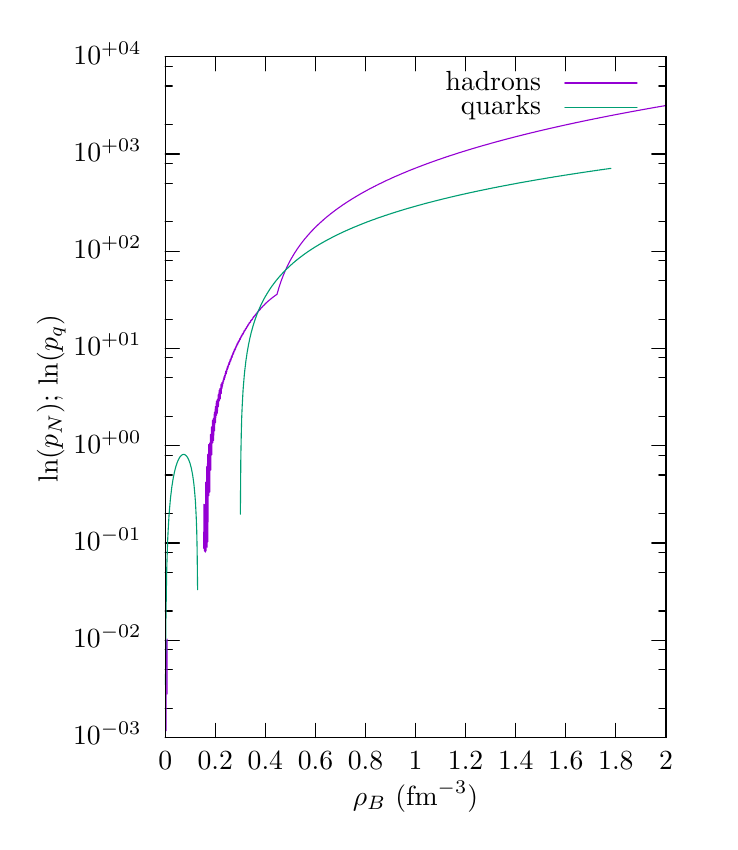
\begin{tikzpicture}[gnuplot]
%% generated with GNUPLOT 5.0p4 (Lua 5.2; terminal rev. 99, script rev. 100)
%% Thu Sep 29 16:33:17 2016
\path (0.000,0.000) rectangle (8.600,10.000);
\gpcolor{color=gp lt color border}
\gpsetlinetype{gp lt border}
\gpsetdashtype{gp dt solid}
\gpsetlinewidth{1.00}
\draw[gp path] (1.688,0.985)--(1.868,0.985);
\draw[gp path] (8.047,0.985)--(7.867,0.985);
\node[gp node right] at (1.504,0.985) {$10^{-03}$};
\draw[gp path] (1.688,1.357)--(1.778,1.357);
\draw[gp path] (8.047,1.357)--(7.957,1.357);
\draw[gp path] (1.688,1.848)--(1.778,1.848);
\draw[gp path] (8.047,1.848)--(7.957,1.848);
\draw[gp path] (1.688,2.100)--(1.778,2.100);
\draw[gp path] (8.047,2.100)--(7.957,2.100);
\draw[gp path] (1.688,2.220)--(1.868,2.220);
\draw[gp path] (8.047,2.220)--(7.867,2.220);
\node[gp node right] at (1.504,2.220) {$10^{-02}$};
\draw[gp path] (1.688,2.592)--(1.778,2.592);
\draw[gp path] (8.047,2.592)--(7.957,2.592);
\draw[gp path] (1.688,3.083)--(1.778,3.083);
\draw[gp path] (8.047,3.083)--(7.957,3.083);
\draw[gp path] (1.688,3.336)--(1.778,3.336);
\draw[gp path] (8.047,3.336)--(7.957,3.336);
\draw[gp path] (1.688,3.455)--(1.868,3.455);
\draw[gp path] (8.047,3.455)--(7.867,3.455);
\node[gp node right] at (1.504,3.455) {$10^{-01}$};
\draw[gp path] (1.688,3.827)--(1.778,3.827);
\draw[gp path] (8.047,3.827)--(7.957,3.827);
\draw[gp path] (1.688,4.319)--(1.778,4.319);
\draw[gp path] (8.047,4.319)--(7.957,4.319);
\draw[gp path] (1.688,4.571)--(1.778,4.571);
\draw[gp path] (8.047,4.571)--(7.957,4.571);
\draw[gp path] (1.688,4.690)--(1.868,4.690);
\draw[gp path] (8.047,4.690)--(7.867,4.690);
\node[gp node right] at (1.504,4.690) {$10^{+00}$};
\draw[gp path] (1.688,5.062)--(1.778,5.062);
\draw[gp path] (8.047,5.062)--(7.957,5.062);
\draw[gp path] (1.688,5.554)--(1.778,5.554);
\draw[gp path] (8.047,5.554)--(7.957,5.554);
\draw[gp path] (1.688,5.806)--(1.778,5.806);
\draw[gp path] (8.047,5.806)--(7.957,5.806);
\draw[gp path] (1.688,5.926)--(1.868,5.926);
\draw[gp path] (8.047,5.926)--(7.867,5.926);
\node[gp node right] at (1.504,5.926) {$10^{+01}$};
\draw[gp path] (1.688,6.297)--(1.778,6.297);
\draw[gp path] (8.047,6.297)--(7.957,6.297);
\draw[gp path] (1.688,6.789)--(1.778,6.789);
\draw[gp path] (8.047,6.789)--(7.957,6.789);
\draw[gp path] (1.688,7.041)--(1.778,7.041);
\draw[gp path] (8.047,7.041)--(7.957,7.041);
\draw[gp path] (1.688,7.161)--(1.868,7.161);
\draw[gp path] (8.047,7.161)--(7.867,7.161);
\node[gp node right] at (1.504,7.161) {$10^{+02}$};
\draw[gp path] (1.688,7.533)--(1.778,7.533);
\draw[gp path] (8.047,7.533)--(7.957,7.533);
\draw[gp path] (1.688,8.024)--(1.778,8.024);
\draw[gp path] (8.047,8.024)--(7.957,8.024);
\draw[gp path] (1.688,8.276)--(1.778,8.276);
\draw[gp path] (8.047,8.276)--(7.957,8.276);
\draw[gp path] (1.688,8.396)--(1.868,8.396);
\draw[gp path] (8.047,8.396)--(7.867,8.396);
\node[gp node right] at (1.504,8.396) {$10^{+03}$};
\draw[gp path] (1.688,8.768)--(1.778,8.768);
\draw[gp path] (8.047,8.768)--(7.957,8.768);
\draw[gp path] (1.688,9.259)--(1.778,9.259);
\draw[gp path] (8.047,9.259)--(7.957,9.259);
\draw[gp path] (1.688,9.511)--(1.778,9.511);
\draw[gp path] (8.047,9.511)--(7.957,9.511);
\draw[gp path] (1.688,9.631)--(1.868,9.631);
\draw[gp path] (8.047,9.631)--(7.867,9.631);
\node[gp node right] at (1.504,9.631) {$10^{+04}$};
\draw[gp path] (1.688,0.985)--(1.688,1.165);
\draw[gp path] (1.688,9.631)--(1.688,9.451);
\node[gp node center] at (1.688,0.677) {$0$};
\draw[gp path] (2.324,0.985)--(2.324,1.165);
\draw[gp path] (2.324,9.631)--(2.324,9.451);
\node[gp node center] at (2.324,0.677) {$0.2$};
\draw[gp path] (2.960,0.985)--(2.960,1.165);
\draw[gp path] (2.960,9.631)--(2.960,9.451);
\node[gp node center] at (2.960,0.677) {$0.4$};
\draw[gp path] (3.596,0.985)--(3.596,1.165);
\draw[gp path] (3.596,9.631)--(3.596,9.451);
\node[gp node center] at (3.596,0.677) {$0.6$};
\draw[gp path] (4.232,0.985)--(4.232,1.165);
\draw[gp path] (4.232,9.631)--(4.232,9.451);
\node[gp node center] at (4.232,0.677) {$0.8$};
\draw[gp path] (4.868,0.985)--(4.868,1.165);
\draw[gp path] (4.868,9.631)--(4.868,9.451);
\node[gp node center] at (4.868,0.677) {$1$};
\draw[gp path] (5.503,0.985)--(5.503,1.165);
\draw[gp path] (5.503,9.631)--(5.503,9.451);
\node[gp node center] at (5.503,0.677) {$1.2$};
\draw[gp path] (6.139,0.985)--(6.139,1.165);
\draw[gp path] (6.139,9.631)--(6.139,9.451);
\node[gp node center] at (6.139,0.677) {$1.4$};
\draw[gp path] (6.775,0.985)--(6.775,1.165);
\draw[gp path] (6.775,9.631)--(6.775,9.451);
\node[gp node center] at (6.775,0.677) {$1.6$};
\draw[gp path] (7.411,0.985)--(7.411,1.165);
\draw[gp path] (7.411,9.631)--(7.411,9.451);
\node[gp node center] at (7.411,0.677) {$1.8$};
\draw[gp path] (8.047,0.985)--(8.047,1.165);
\draw[gp path] (8.047,9.631)--(8.047,9.451);
\node[gp node center] at (8.047,0.677) {$2$};
\draw[gp path] (1.688,9.631)--(1.688,0.985)--(8.047,0.985)--(8.047,9.631)--cycle;
\node[gp node center,rotate=-270] at (0.246,5.308) {$\ln(p_N)$; $\ln(p_q)$};
\node[gp node center] at (4.867,0.215) {$\rho_B$ ($\rm{fm}^{-3}$)};
\node[gp node right] at (6.579,9.297) {hadrons};
\gpcolor{rgb color={0.580,0.000,0.827}}
\draw[gp path] (6.763,9.297)--(7.679,9.297);
\draw[gp path] (1.698,1.070)--(1.700,1.846)--(1.702,2.220);
\draw[gp path] (1.710,1.535)--(1.712,2.235);
\draw[gp path] (2.177,3.388)--(2.179,3.947);
\draw[gp path] (2.187,3.351)--(2.189,3.943);
\draw[gp path] (2.198,3.339)--(2.200,3.948)--(2.202,4.228);
\draw[gp path] (2.208,3.356)--(2.210,3.962)--(2.213,4.241)--(2.215,4.425);
\draw[gp path] (2.219,3.402)--(2.221,3.985)--(2.223,4.260)--(2.225,4.442)--(2.227,4.578)%
  --(2.229,3.471)--(2.232,4.017)--(2.234,4.284)--(2.236,4.462)--(2.238,4.597)--(2.240,4.705)%
  --(2.242,4.057)--(2.244,4.313)--(2.246,4.486)--(2.249,4.618)--(2.251,4.724)--(2.253,4.103)%
  --(2.255,4.346)--(2.257,4.513)--(2.259,4.642)--(2.261,4.746)--(2.263,4.834)--(2.266,4.383)%
  --(2.268,4.544)--(2.270,4.668)--(2.272,4.770)--(2.274,4.855)--(2.276,4.930)--(2.278,4.576)%
  --(2.280,4.696)--(2.282,4.795)--(2.285,4.879)--(2.287,4.952)--(2.289,5.016)--(2.291,4.727)%
  --(2.293,4.822)--(2.295,4.903)--(2.297,4.975)--(2.299,5.038)--(2.302,4.758)--(2.304,4.850)%
  --(2.306,4.929)--(2.308,4.999)--(2.310,5.060)--(2.312,5.116)--(2.314,4.880)--(2.316,4.957)%
  --(2.318,5.024)--(2.321,5.084)--(2.323,5.138)--(2.325,5.188)--(2.327,4.985)--(2.329,5.050)%
  --(2.331,5.108)--(2.333,5.161)--(2.335,5.210)--(2.338,5.255)--(2.340,5.077)--(2.342,5.134)%
  --(2.344,5.185)--(2.346,5.233)--(2.348,5.276)--(2.350,5.105)--(2.352,5.160)--(2.355,5.210)%
  --(2.357,5.256)--(2.359,5.299)--(2.361,5.338)--(2.363,5.186)--(2.365,5.235)--(2.367,5.280)%
  --(2.369,5.321)--(2.371,5.360)--(2.374,5.397)--(2.376,5.261)--(2.378,5.304)--(2.380,5.345)%
  --(2.382,5.383)--(2.384,5.418)--(2.386,5.287)--(2.388,5.329)--(2.391,5.368)--(2.393,5.405)%
  --(2.395,5.440)--(2.397,5.473)--(2.399,5.354)--(2.401,5.392)--(2.403,5.428)--(2.405,5.462)%
  --(2.408,5.494)--(2.410,5.420)--(2.412,5.454)--(2.414,5.487)--(2.416,5.449)--(2.418,5.482)%
  --(2.420,5.514)--(2.422,5.478)--(2.424,5.510)--(2.427,5.540)--(2.429,5.505)--(2.431,5.536)%
  --(2.433,5.565)--(2.435,5.532)--(2.437,5.562)--(2.439,5.529)--(2.441,5.559)--(2.444,5.587)%
  --(2.446,5.555)--(2.448,5.584)--(2.450,5.612)--(2.452,5.581)--(2.454,5.609)--(2.456,5.636)%
  --(2.458,5.607)--(2.460,5.633)--(2.463,5.604)--(2.465,5.631)--(2.467,5.657)--(2.469,5.629)%
  --(2.471,5.655)--(2.473,5.680)--(2.475,5.654)--(2.477,5.679)--(2.480,5.703)--(2.482,5.677)%
  --(2.484,5.702)--(2.486,5.676)--(2.488,5.701)--(2.490,5.724)--(2.492,5.700)--(2.494,5.723)%
  --(2.497,5.746)--(2.499,5.722)--(2.501,5.745)--(2.503,5.722)--(2.505,5.745)--(2.507,5.767)%
  --(2.509,5.744)--(2.511,5.767)--(2.513,5.788)--(2.516,5.767)--(2.518,5.788)--(2.520,5.766)%
  --(2.522,5.788)--(2.524,5.809)--(2.526,5.788)--(2.528,5.810)--(2.530,5.830)--(2.533,5.810)%
  --(2.535,5.830)--(2.537,5.810)--(2.539,5.831)--(2.541,5.851)--(2.543,5.831)--(2.545,5.851)%
  --(2.547,5.871)--(2.550,5.852)--(2.552,5.872)--(2.554,5.853)--(2.556,5.872)--(2.558,5.891)%
  --(2.560,5.873)--(2.562,5.892)--(2.564,5.911)--(2.566,5.894)--(2.569,5.912)--(2.571,5.895)%
  --(2.573,5.913)--(2.575,5.931)--(2.577,5.915)--(2.579,5.933)--(2.581,5.916)--(2.583,5.934)%
  --(2.586,5.952)--(2.588,5.936)--(2.590,5.953)--(2.592,5.970)--(2.594,5.955)--(2.596,5.972)%
  --(2.598,5.957)--(2.600,5.974)--(2.602,5.991)--(2.605,5.976)--(2.607,5.992)--(2.609,5.978)%
  --(2.611,5.995)--(2.613,6.011)--(2.615,5.997)--(2.617,6.013)--(2.619,5.999)--(2.622,6.015)%
  --(2.624,6.031)--(2.626,6.017)--(2.628,6.033)--(2.630,6.020)--(2.632,6.036)--(2.634,6.051)%
  --(2.636,6.038)--(2.639,6.053)--(2.641,6.041)--(2.643,6.056)--(2.645,6.071)--(2.647,6.059)%
  --(2.649,6.074)--(2.651,6.061)--(2.653,6.076)--(2.655,6.091)--(2.658,6.079)--(2.660,6.094)%
  --(2.662,6.082)--(2.664,6.097)--(2.666,6.111)--(2.668,6.100)--(2.670,6.114)--(2.672,6.103)%
  --(2.675,6.117)--(2.677,6.106)--(2.679,6.120)--(2.681,6.134)--(2.683,6.123)--(2.685,6.137)%
  --(2.687,6.127)--(2.689,6.141)--(2.691,6.154)--(2.694,6.144)--(2.696,6.157)--(2.698,6.147)%
  --(2.700,6.161)--(2.702,6.151)--(2.704,6.164)--(2.706,6.177)--(2.708,6.168)--(2.711,6.181)%
  --(2.713,6.171)--(2.715,6.185)--(2.717,6.175)--(2.719,6.188)--(2.721,6.201)--(2.723,6.192)%
  --(2.725,6.205)--(2.728,6.196)--(2.730,6.208)--(2.732,6.200)--(2.734,6.212)--(2.736,6.225)%
  --(2.738,6.216)--(2.740,6.229)--(2.742,6.220)--(2.744,6.233)--(2.747,6.224)--(2.749,6.237)%
  --(2.751,6.249)--(2.753,6.241)--(2.755,6.253)--(2.757,6.245)--(2.759,6.257)--(2.761,6.249)%
  --(2.764,6.261)--(2.766,6.253)--(2.768,6.265)--(2.770,6.258)--(2.772,6.270)--(2.774,6.281)%
  --(2.776,6.274)--(2.778,6.286)--(2.781,6.278)--(2.783,6.290)--(2.785,6.283)--(2.787,6.294)%
  --(2.789,6.288)--(2.791,6.299)--(2.793,6.292)--(2.795,6.304)--(2.797,6.297)--(2.800,6.308)%
  --(2.802,6.319)--(2.804,6.313)--(2.806,6.324)--(2.808,6.318)--(2.810,6.329)--(2.812,6.323)%
  --(2.814,6.334)--(2.817,6.328)--(2.819,6.338)--(2.821,6.333)--(2.823,6.343)--(2.825,6.338)%
  --(2.827,6.348)--(2.829,6.343)--(2.831,6.353)--(2.833,6.348)--(2.836,6.359)--(2.838,6.353)%
  --(2.840,6.364)--(2.842,6.358)--(2.844,6.369)--(2.846,6.364)--(2.848,6.374)--(2.850,6.369)%
  --(2.853,6.379)--(2.855,6.375)--(2.857,6.385)--(2.859,6.380)--(2.861,6.390)--(2.863,6.386)%
  --(2.865,6.396)--(2.867,6.391)--(2.870,6.401)--(2.872,6.397)--(2.874,6.407)--(2.876,6.403)%
  --(2.878,6.413)--(2.880,6.408)--(2.882,6.418)--(2.884,6.414)--(2.886,6.410)--(2.889,6.420)%
  --(2.891,6.416)--(2.893,6.426)--(2.895,6.422)--(2.897,6.432)--(2.899,6.428)--(2.901,6.438)%
  --(2.903,6.435)--(2.906,6.444)--(2.908,6.441)--(2.910,6.441)--(2.912,6.444)--(2.914,6.447)%
  --(2.916,6.450)--(2.918,6.453)--(2.920,6.456)--(2.923,6.453)--(2.925,6.457)--(2.927,6.460)%
  --(2.929,6.463)--(2.931,6.467)--(2.933,6.470)--(2.935,6.467)--(2.937,6.471)--(2.939,6.474)%
  --(2.942,6.477)--(2.944,6.475)--(2.946,6.478)--(2.948,6.482)--(2.950,6.485)--(2.952,6.489)%
  --(2.954,6.487)--(2.956,6.490)--(2.959,6.494)--(2.961,6.492)--(2.963,6.496)--(2.965,6.499)%
  --(2.967,6.503)--(2.969,6.501)--(2.971,6.505)--(2.973,6.509)--(2.975,6.507)--(2.978,6.511)%
  --(2.980,6.515)--(2.982,6.514)--(2.984,6.518)--(2.986,6.517)--(2.988,6.520)--(2.990,6.524)%
  --(2.992,6.524)--(2.995,6.528)--(2.997,6.527)--(2.999,6.531)--(3.001,6.530)--(3.003,6.534)%
  --(3.005,6.534)--(3.007,6.538)--(3.009,6.538)--(3.012,6.542)--(3.014,6.542)--(3.016,6.542)%
  --(3.018,6.547)--(3.020,6.547)--(3.022,6.551)--(3.024,6.551)--(3.026,6.552)--(3.028,6.556)%
  --(3.031,6.557)--(3.033,6.558)--(3.035,6.559)--(3.037,6.563)--(3.039,6.564)--(3.041,6.565)%
  --(3.043,6.567)--(3.045,6.568)--(3.048,6.569)--(3.050,6.571)--(3.052,6.572)--(3.054,6.574)%
  --(3.056,6.577)--(3.058,6.579)--(3.060,6.579)--(3.062,6.582)--(3.064,6.582)--(3.067,6.585)%
  --(3.069,6.586)--(3.071,6.587)--(3.073,6.589)--(3.075,6.591)--(3.077,6.593)--(3.079,6.594)%
  --(3.081,6.596)--(3.084,6.597)--(3.086,6.598)--(3.088,6.600)--(3.090,6.601)--(3.092,6.603)%
  --(3.094,6.604)--(3.096,6.606)--(3.098,6.607)--(3.101,6.609)--(3.103,6.610)--(3.105,6.611)%
  --(3.107,6.613)--(3.109,6.619)--(3.111,6.627)--(3.113,6.634)--(3.115,6.642)--(3.117,6.649)%
  --(3.120,6.657)--(3.122,6.664)--(3.124,6.671)--(3.126,6.678)--(3.128,6.685)--(3.130,6.692)%
  --(3.132,6.699)--(3.134,6.706)--(3.137,6.713)--(3.139,6.719)--(3.141,6.726)--(3.143,6.732)%
  --(3.145,6.739)--(3.147,6.745)--(3.149,6.751)--(3.151,6.757)--(3.154,6.764)--(3.156,6.770)%
  --(3.158,6.776)--(3.160,6.782)--(3.162,6.788)--(3.164,6.793)--(3.166,6.799)--(3.168,6.805)%
  --(3.170,6.811)--(3.173,6.816)--(3.175,6.822)--(3.177,6.827)--(3.179,6.833)--(3.181,6.838)%
  --(3.183,6.844)--(3.185,6.849)--(3.187,6.854)--(3.190,6.860)--(3.192,6.865)--(3.194,6.870)%
  --(3.196,6.875)--(3.198,6.880)--(3.200,6.885)--(3.202,6.890)--(3.204,6.895)--(3.206,6.900)%
  --(3.209,6.905)--(3.211,6.910)--(3.213,6.915)--(3.215,6.919)--(3.217,6.924)--(3.219,6.929)%
  --(3.221,6.933)--(3.223,6.938)--(3.226,6.943)--(3.228,6.947)--(3.230,6.952)--(3.232,6.956)%
  --(3.234,6.961)--(3.236,6.965)--(3.238,6.970)--(3.240,6.974)--(3.243,6.978)--(3.245,6.983)%
  --(3.247,6.987)--(3.249,6.991)--(3.251,6.995)--(3.253,7.000)--(3.255,7.004)--(3.257,7.008)%
  --(3.259,7.012)--(3.262,7.016)--(3.264,7.020)--(3.266,7.024)--(3.268,7.028)--(3.270,7.032)%
  --(3.272,7.036)--(3.274,7.040)--(3.276,7.044)--(3.279,7.048)--(3.281,7.052)--(3.283,7.056)%
  --(3.285,7.059)--(3.287,7.063)--(3.289,7.067)--(3.291,7.071)--(3.293,7.074)--(3.295,7.078)%
  --(3.298,7.082)--(3.300,7.085)--(3.302,7.089)--(3.304,7.093)--(3.306,7.096)--(3.308,7.100)%
  --(3.310,7.103)--(3.312,7.107)--(3.315,7.111)--(3.317,7.114)--(3.319,7.118)--(3.321,7.121)%
  --(3.323,7.124)--(3.325,7.128)--(3.327,7.131)--(3.329,7.135)--(3.332,7.138)--(3.334,7.141)%
  --(3.336,7.145)--(3.338,7.148)--(3.340,7.151)--(3.342,7.155)--(3.344,7.158)--(3.346,7.161)%
  --(3.348,7.165)--(3.351,7.168)--(3.353,7.171)--(3.355,7.174)--(3.357,7.177)--(3.359,7.181)%
  --(3.361,7.184)--(3.363,7.187)--(3.365,7.190)--(3.368,7.193)--(3.370,7.196)--(3.372,7.199)%
  --(3.374,7.202)--(3.376,7.205)--(3.378,7.208)--(3.380,7.212)--(3.382,7.215)--(3.385,7.218)%
  --(3.387,7.221)--(3.389,7.223)--(3.391,7.226)--(3.393,7.229)--(3.395,7.232)--(3.397,7.235)%
  --(3.399,7.238)--(3.401,7.241)--(3.404,7.244)--(3.406,7.247)--(3.408,7.250)--(3.410,7.253)%
  --(3.412,7.255)--(3.414,7.258)--(3.416,7.261)--(3.418,7.264)--(3.421,7.267)--(3.423,7.269)%
  --(3.425,7.272)--(3.427,7.275)--(3.429,7.278)--(3.431,7.280)--(3.433,7.283)--(3.435,7.286)%
  --(3.437,7.289)--(3.440,7.291)--(3.442,7.294)--(3.444,7.297)--(3.446,7.299)--(3.448,7.302)%
  --(3.450,7.305)--(3.452,7.307)--(3.454,7.310)--(3.457,7.312)--(3.459,7.315)--(3.461,7.318)%
  --(3.463,7.320)--(3.465,7.323)--(3.467,7.325)--(3.469,7.328)--(3.471,7.330)--(3.474,7.333)%
  --(3.476,7.335)--(3.478,7.338)--(3.480,7.340)--(3.482,7.343)--(3.484,7.345)--(3.486,7.348)%
  --(3.488,7.350)--(3.490,7.353)--(3.493,7.355)--(3.495,7.358)--(3.497,7.360)--(3.499,7.363)%
  --(3.501,7.365)--(3.503,7.367)--(3.505,7.370)--(3.507,7.372)--(3.510,7.375)--(3.512,7.377)%
  --(3.514,7.379)--(3.516,7.382)--(3.518,7.384)--(3.520,7.386)--(3.522,7.389)--(3.524,7.391)%
  --(3.527,7.393)--(3.529,7.396)--(3.531,7.398)--(3.533,7.400)--(3.535,7.403)--(3.537,7.405)%
  --(3.539,7.407)--(3.541,7.410)--(3.543,7.412)--(3.546,7.414)--(3.548,7.416)--(3.550,7.419)%
  --(3.552,7.421)--(3.554,7.423)--(3.556,7.425)--(3.558,7.427)--(3.560,7.430)--(3.563,7.432)%
  --(3.565,7.434)--(3.567,7.436)--(3.569,7.438)--(3.571,7.441)--(3.573,7.443)--(3.575,7.445)%
  --(3.577,7.447)--(3.579,7.449)--(3.582,7.451)--(3.584,7.454)--(3.586,7.456)--(3.588,7.458)%
  --(3.590,7.460)--(3.592,7.462)--(3.594,7.464)--(3.596,7.466)--(3.599,7.468)--(3.601,7.470)%
  --(3.603,7.473)--(3.605,7.475)--(3.607,7.477)--(3.609,7.479)--(3.611,7.481)--(3.613,7.483)%
  --(3.616,7.485)--(3.618,7.487)--(3.620,7.489)--(3.622,7.491)--(3.624,7.493)--(3.626,7.495)%
  --(3.628,7.497)--(3.630,7.499)--(3.632,7.501)--(3.635,7.503)--(3.637,7.505)--(3.639,7.507)%
  --(3.641,7.509)--(3.643,7.511)--(3.645,7.513)--(3.647,7.515)--(3.649,7.517)--(3.652,7.519)%
  --(3.654,7.521)--(3.656,7.523)--(3.658,7.525)--(3.660,7.527)--(3.662,7.528)--(3.664,7.530)%
  --(3.666,7.532)--(3.668,7.534)--(3.671,7.536)--(3.673,7.538)--(3.675,7.540)--(3.677,7.542)%
  --(3.679,7.544)--(3.681,7.546)--(3.683,7.548)--(3.685,7.549)--(3.688,7.551)--(3.690,7.553)%
  --(3.692,7.555)--(3.694,7.557)--(3.696,7.559)--(3.698,7.561)--(3.700,7.562)--(3.702,7.564)%
  --(3.705,7.566)--(3.707,7.568)--(3.709,7.570)--(3.711,7.572)--(3.713,7.573)--(3.715,7.575)%
  --(3.717,7.577)--(3.719,7.579)--(3.721,7.581)--(3.724,7.582)--(3.726,7.584)--(3.728,7.586)%
  --(3.730,7.588)--(3.732,7.589)--(3.734,7.591)--(3.736,7.593)--(3.738,7.595)--(3.741,7.597)%
  --(3.743,7.598)--(3.745,7.600)--(3.747,7.602)--(3.749,7.604)--(3.751,7.605)--(3.753,7.607)%
  --(3.755,7.609)--(3.758,7.610)--(3.760,7.612)--(3.762,7.614)--(3.764,7.616)--(3.766,7.617)%
  --(3.768,7.619)--(3.770,7.621)--(3.772,7.622)--(3.774,7.624)--(3.777,7.626)--(3.779,7.628)%
  --(3.781,7.629)--(3.783,7.631)--(3.785,7.633)--(3.787,7.634)--(3.789,7.636)--(3.791,7.638)%
  --(3.794,7.639)--(3.796,7.641)--(3.798,7.643)--(3.800,7.644)--(3.802,7.646)--(3.804,7.648)%
  --(3.806,7.649)--(3.808,7.651)--(3.810,7.652)--(3.813,7.654)--(3.815,7.656)--(3.817,7.657)%
  --(3.819,7.659)--(3.821,7.661)--(3.823,7.662)--(3.825,7.664)--(3.827,7.665)--(3.830,7.667)%
  --(3.832,7.669)--(3.834,7.670)--(3.836,7.672)--(3.838,7.673)--(3.840,7.675)--(3.842,7.677)%
  --(3.844,7.678)--(3.847,7.680)--(3.849,7.681)--(3.851,7.683)--(3.853,7.684)--(3.855,7.686)%
  --(3.857,7.688)--(3.859,7.689)--(3.861,7.691)--(3.863,7.692)--(3.866,7.694)--(3.868,7.695)%
  --(3.870,7.697)--(3.872,7.698)--(3.874,7.700)--(3.876,7.701)--(3.878,7.703)--(3.880,7.705)%
  --(3.883,7.706)--(3.885,7.708)--(3.887,7.709)--(3.889,7.711)--(3.891,7.712)--(3.893,7.714)%
  --(3.895,7.715)--(3.897,7.717)--(3.900,7.718)--(3.902,7.720)--(3.904,7.721)--(3.906,7.723)%
  --(3.908,7.724)--(3.910,7.726)--(3.912,7.727)--(3.914,7.729)--(3.916,7.730)--(3.919,7.732)%
  --(3.921,7.733)--(3.923,7.734)--(3.925,7.736)--(3.927,7.737)--(3.929,7.739)--(3.931,7.740)%
  --(3.933,7.742)--(3.936,7.743)--(3.938,7.745)--(3.940,7.746)--(3.942,7.748)--(3.944,7.749)%
  --(3.946,7.750)--(3.948,7.752)--(3.950,7.753)--(3.952,7.755)--(3.955,7.756)--(3.957,7.758)%
  --(3.959,7.759)--(3.961,7.760)--(3.963,7.762)--(3.965,7.763)--(3.967,7.765)--(3.969,7.766)%
  --(3.972,7.768)--(3.974,7.769)--(3.976,7.770)--(3.978,7.772)--(3.980,7.773)--(3.982,7.775)%
  --(3.984,7.776)--(3.986,7.777)--(3.989,7.779)--(3.991,7.780)--(3.993,7.782)--(3.995,7.783)%
  --(3.997,7.784)--(3.999,7.786)--(4.001,7.787)--(4.003,7.788)--(4.005,7.790)--(4.008,7.791)%
  --(4.010,7.793)--(4.012,7.794)--(4.014,7.795)--(4.016,7.797)--(4.018,7.798)--(4.020,7.799)%
  --(4.022,7.801)--(4.025,7.802)--(4.027,7.803)--(4.029,7.805)--(4.031,7.806)--(4.033,7.807)%
  --(4.035,7.809)--(4.037,7.810)--(4.039,7.811)--(4.041,7.813)--(4.044,7.814)--(4.046,7.815)%
  --(4.048,7.817)--(4.050,7.818)--(4.052,7.819)--(4.054,7.821)--(4.056,7.822)--(4.058,7.823)%
  --(4.061,7.825)--(4.063,7.826)--(4.065,7.827)--(4.067,7.829)--(4.069,7.830)--(4.071,7.831)%
  --(4.073,7.832)--(4.075,7.834)--(4.078,7.835)--(4.080,7.836)--(4.082,7.838)--(4.084,7.839)%
  --(4.086,7.840)--(4.088,7.842)--(4.090,7.843)--(4.092,7.844)--(4.094,7.845)--(4.097,7.847)%
  --(4.099,7.848)--(4.101,7.849)--(4.103,7.850)--(4.105,7.852)--(4.107,7.853)--(4.109,7.854)%
  --(4.111,7.856)--(4.114,7.857)--(4.116,7.858)--(4.118,7.859)--(4.120,7.861)--(4.122,7.862)%
  --(4.124,7.863)--(4.126,7.864)--(4.128,7.866)--(4.131,7.867)--(4.133,7.868)--(4.135,7.869)%
  --(4.137,7.871)--(4.139,7.872)--(4.141,7.873)--(4.143,7.874)--(4.145,7.876)--(4.147,7.877)%
  --(4.150,7.878)--(4.152,7.879)--(4.154,7.880)--(4.156,7.882)--(4.158,7.883)--(4.160,7.884)%
  --(4.162,7.885)--(4.164,7.887)--(4.167,7.888)--(4.169,7.889)--(4.171,7.890)--(4.173,7.891)%
  --(4.175,7.893)--(4.177,7.894)--(4.179,7.895)--(4.181,7.896)--(4.183,7.897)--(4.186,7.899)%
  --(4.188,7.900)--(4.190,7.901)--(4.192,7.902)--(4.194,7.903)--(4.196,7.905)--(4.198,7.906)%
  --(4.200,7.907)--(4.203,7.908)--(4.205,7.909)--(4.207,7.911)--(4.209,7.912)--(4.211,7.913)%
  --(4.213,7.914)--(4.215,7.915)--(4.217,7.916)--(4.220,7.918)--(4.222,7.919)--(4.224,7.920)%
  --(4.226,7.921)--(4.228,7.922)--(4.230,7.923)--(4.232,7.925)--(4.234,7.926)--(4.236,7.927)%
  --(4.239,7.928)--(4.241,7.929)--(4.243,7.930)--(4.245,7.932)--(4.247,7.933)--(4.249,7.934)%
  --(4.251,7.935)--(4.253,7.936)--(4.256,7.937)--(4.258,7.938)--(4.260,7.940)--(4.262,7.941)%
  --(4.264,7.942)--(4.266,7.943)--(4.268,7.944)--(4.270,7.945)--(4.273,7.946)--(4.275,7.948)%
  --(4.277,7.949)--(4.279,7.950)--(4.281,7.951)--(4.283,7.952)--(4.285,7.953)--(4.287,7.954)%
  --(4.289,7.955)--(4.292,7.957)--(4.294,7.958)--(4.296,7.959)--(4.298,7.960)--(4.300,7.961)%
  --(4.302,7.962)--(4.304,7.963)--(4.306,7.964)--(4.309,7.965)--(4.311,7.967)--(4.313,7.968)%
  --(4.315,7.969)--(4.317,7.970)--(4.319,7.971)--(4.321,7.972)--(4.323,7.973)--(4.325,7.974)%
  --(4.328,7.975)--(4.330,7.976)--(4.332,7.978)--(4.334,7.979)--(4.336,7.980)--(4.338,7.981)%
  --(4.340,7.982)--(4.342,7.983)--(4.345,7.984)--(4.347,7.985)--(4.349,7.986)--(4.351,7.987)%
  --(4.353,7.988)--(4.355,7.989)--(4.357,7.990)--(4.359,7.992)--(4.362,7.993)--(4.364,7.994)%
  --(4.366,7.995)--(4.368,7.996)--(4.370,7.997)--(4.372,7.998)--(4.374,7.999)--(4.376,8.000)%
  --(4.378,8.001)--(4.381,8.002)--(4.383,8.003)--(4.385,8.004)--(4.387,8.005)--(4.389,8.006)%
  --(4.391,8.008)--(4.393,8.009)--(4.395,8.010)--(4.398,8.011)--(4.400,8.012)--(4.402,8.013)%
  --(4.404,8.014)--(4.406,8.015)--(4.408,8.016)--(4.410,8.017)--(4.412,8.018)--(4.414,8.019)%
  --(4.417,8.020)--(4.419,8.021)--(4.421,8.022)--(4.423,8.023)--(4.425,8.024)--(4.427,8.025)%
  --(4.429,8.026)--(4.431,8.027)--(4.434,8.028)--(4.436,8.029)--(4.438,8.030)--(4.440,8.031)%
  --(4.442,8.032)--(4.444,8.033)--(4.446,8.034)--(4.448,8.035)--(4.451,8.037)--(4.453,8.038)%
  --(4.455,8.039)--(4.457,8.040)--(4.459,8.041)--(4.461,8.042)--(4.463,8.043)--(4.465,8.044)%
  --(4.467,8.045)--(4.470,8.046)--(4.472,8.047)--(4.474,8.048)--(4.476,8.049)--(4.478,8.050)%
  --(4.480,8.051)--(4.482,8.052)--(4.484,8.053)--(4.487,8.054)--(4.489,8.055)--(4.491,8.056)%
  --(4.493,8.057)--(4.495,8.058)--(4.497,8.059)--(4.499,8.060)--(4.501,8.061)--(4.504,8.062)%
  --(4.506,8.063)--(4.508,8.064)--(4.510,8.065)--(4.512,8.066)--(4.514,8.067)--(4.516,8.068)%
  --(4.518,8.068)--(4.520,8.069)--(4.523,8.070)--(4.525,8.071)--(4.527,8.072)--(4.529,8.073)%
  --(4.531,8.074)--(4.533,8.075)--(4.535,8.076)--(4.537,8.077)--(4.540,8.078)--(4.542,8.079)%
  --(4.544,8.080)--(4.546,8.081)--(4.548,8.082)--(4.550,8.083)--(4.552,8.084)--(4.554,8.085)%
  --(4.556,8.086)--(4.559,8.087)--(4.561,8.088)--(4.563,8.089)--(4.565,8.090)--(4.567,8.091)%
  --(4.569,8.092)--(4.571,8.093)--(4.573,8.094)--(4.576,8.095)--(4.578,8.096)--(4.580,8.096)%
  --(4.582,8.097)--(4.584,8.098)--(4.586,8.099)--(4.588,8.100)--(4.590,8.101)--(4.593,8.102)%
  --(4.595,8.103)--(4.597,8.104)--(4.599,8.105)--(4.601,8.106)--(4.603,8.107)--(4.605,8.108)%
  --(4.607,8.109)--(4.609,8.110)--(4.612,8.111)--(4.614,8.112)--(4.616,8.112)--(4.618,8.113)%
  --(4.620,8.114)--(4.622,8.115)--(4.624,8.116)--(4.626,8.117)--(4.629,8.118)--(4.631,8.119)%
  --(4.633,8.120)--(4.635,8.121)--(4.637,8.122)--(4.639,8.123)--(4.641,8.124)--(4.643,8.125)%
  --(4.646,8.125)--(4.648,8.126)--(4.650,8.127)--(4.652,8.128)--(4.654,8.129)--(4.656,8.130)%
  --(4.658,8.131)--(4.660,8.132)--(4.662,8.133)--(4.665,8.134)--(4.667,8.135)--(4.669,8.135)%
  --(4.671,8.136)--(4.673,8.137)--(4.675,8.138)--(4.677,8.139)--(4.679,8.140)--(4.682,8.141)%
  --(4.684,8.142)--(4.686,8.143)--(4.688,8.144)--(4.690,8.145)--(4.692,8.145)--(4.694,8.146)%
  --(4.696,8.147)--(4.698,8.148)--(4.701,8.149)--(4.703,8.150)--(4.705,8.151)--(4.707,8.152)%
  --(4.709,8.153)--(4.711,8.153)--(4.713,8.154)--(4.715,8.155)--(4.718,8.156)--(4.720,8.157)%
  --(4.722,8.158)--(4.724,8.159)--(4.726,8.160)--(4.728,8.161)--(4.730,8.161)--(4.732,8.162)%
  --(4.735,8.163)--(4.737,8.164)--(4.739,8.165)--(4.741,8.166)--(4.743,8.167)--(4.745,8.168)%
  --(4.747,8.168)--(4.749,8.169)--(4.751,8.170)--(4.754,8.171)--(4.756,8.172)--(4.758,8.173)%
  --(4.760,8.174)--(4.762,8.175)--(4.764,8.175)--(4.766,8.176)--(4.768,8.177)--(4.771,8.178)%
  --(4.773,8.179)--(4.775,8.180)--(4.777,8.181)--(4.779,8.182)--(4.781,8.182)--(4.783,8.183)%
  --(4.785,8.184)--(4.787,8.185)--(4.790,8.186)--(4.792,8.187)--(4.794,8.188)--(4.796,8.188)%
  --(4.798,8.189)--(4.800,8.190)--(4.802,8.191)--(4.804,8.192)--(4.807,8.193)--(4.809,8.194)%
  --(4.811,8.194)--(4.813,8.195)--(4.815,8.196)--(4.817,8.197)--(4.819,8.198)--(4.821,8.199)%
  --(4.824,8.199)--(4.826,8.200)--(4.828,8.201)--(4.830,8.202)--(4.832,8.203)--(4.834,8.204)%
  --(4.836,8.205)--(4.838,8.205)--(4.840,8.206)--(4.843,8.207)--(4.845,8.208)--(4.847,8.209)%
  --(4.849,8.210)--(4.851,8.210)--(4.853,8.211)--(4.855,8.212)--(4.857,8.213)--(4.860,8.214)%
  --(4.862,8.215)--(4.864,8.215)--(4.866,8.216)--(4.868,8.217)--(4.870,8.218)--(4.872,8.219)%
  --(4.874,8.220)--(4.877,8.220)--(4.879,8.221)--(4.881,8.222)--(4.883,8.223)--(4.885,8.224)%
  --(4.887,8.224)--(4.889,8.225)--(4.891,8.226)--(4.893,8.227)--(4.896,8.228)--(4.898,8.229)%
  --(4.900,8.229)--(4.902,8.230)--(4.904,8.231)--(4.906,8.232)--(4.908,8.233)--(4.910,8.233)%
  --(4.913,8.234)--(4.915,8.235)--(4.917,8.236)--(4.919,8.237)--(4.921,8.238)--(4.923,8.238)%
  --(4.925,8.239)--(4.927,8.240)--(4.929,8.241)--(4.932,8.242)--(4.934,8.242)--(4.936,8.243)%
  --(4.938,8.244)--(4.940,8.245)--(4.942,8.246)--(4.944,8.246)--(4.946,8.247)--(4.949,8.248)%
  --(4.951,8.249)--(4.953,8.250)--(4.955,8.250)--(4.957,8.251)--(4.959,8.252)--(4.961,8.253)%
  --(4.963,8.254)--(4.966,8.254)--(4.968,8.255)--(4.970,8.256)--(4.972,8.257)--(4.974,8.258)%
  --(4.976,8.258)--(4.978,8.259)--(4.980,8.260)--(4.982,8.261)--(4.985,8.262)--(4.987,8.262)%
  --(4.989,8.263)--(4.991,8.264)--(4.993,8.265)--(4.995,8.265)--(4.997,8.266)--(4.999,8.267)%
  --(5.002,8.268)--(5.004,8.269)--(5.006,8.269)--(5.008,8.270)--(5.010,8.271)--(5.012,8.272)%
  --(5.014,8.273)--(5.016,8.273)--(5.019,8.274)--(5.021,8.275)--(5.023,8.276)--(5.025,8.276)%
  --(5.027,8.277)--(5.029,8.278)--(5.031,8.279)--(5.033,8.279)--(5.035,8.280)--(5.038,8.281)%
  --(5.040,8.282)--(5.042,8.283)--(5.044,8.283)--(5.046,8.284)--(5.048,8.285)--(5.050,8.286)%
  --(5.052,8.286)--(5.055,8.287)--(5.057,8.288)--(5.059,8.289)--(5.061,8.290)--(5.063,8.290)%
  --(5.065,8.291)--(5.067,8.292)--(5.069,8.293)--(5.071,8.293)--(5.074,8.294)--(5.076,8.295)%
  --(5.078,8.296)--(5.080,8.296)--(5.082,8.297)--(5.084,8.298)--(5.086,8.299)--(5.088,8.299)%
  --(5.091,8.300)--(5.093,8.301)--(5.095,8.302)--(5.097,8.302)--(5.099,8.303)--(5.101,8.304)%
  --(5.103,8.305)--(5.105,8.305)--(5.108,8.306)--(5.110,8.307)--(5.112,8.308)--(5.114,8.308)%
  --(5.116,8.309)--(5.118,8.310)--(5.120,8.311)--(5.122,8.311)--(5.124,8.312)--(5.127,8.313)%
  --(5.129,8.314)--(5.131,8.314)--(5.133,8.315)--(5.135,8.316)--(5.137,8.317)--(5.139,8.317)%
  --(5.141,8.318)--(5.144,8.319)--(5.146,8.320)--(5.148,8.320)--(5.150,8.321)--(5.152,8.322)%
  --(5.154,8.323)--(5.156,8.323)--(5.158,8.324)--(5.160,8.325)--(5.163,8.326)--(5.165,8.326)%
  --(5.167,8.327)--(5.169,8.328)--(5.171,8.328)--(5.173,8.329)--(5.175,8.330)--(5.177,8.331)%
  --(5.180,8.331)--(5.182,8.332)--(5.184,8.333)--(5.186,8.334)--(5.188,8.334)--(5.190,8.335)%
  --(5.192,8.336)--(5.194,8.336)--(5.197,8.337)--(5.199,8.338)--(5.201,8.339)--(5.203,8.339)%
  --(5.205,8.340)--(5.207,8.341)--(5.209,8.342)--(5.211,8.342)--(5.213,8.343)--(5.216,8.344)%
  --(5.218,8.344)--(5.220,8.345)--(5.222,8.346)--(5.224,8.347)--(5.226,8.347)--(5.228,8.348)%
  --(5.230,8.349)--(5.233,8.349)--(5.235,8.350)--(5.237,8.351)--(5.239,8.352)--(5.241,8.352)%
  --(5.243,8.353)--(5.245,8.354)--(5.247,8.354)--(5.250,8.355)--(5.252,8.356)--(5.254,8.357)%
  --(5.256,8.357)--(5.258,8.358)--(5.260,8.359)--(5.262,8.359)--(5.264,8.360)--(5.266,8.361)%
  --(5.269,8.362)--(5.271,8.362)--(5.273,8.363)--(5.275,8.364)--(5.277,8.364)--(5.279,8.365)%
  --(5.281,8.366)--(5.283,8.367)--(5.286,8.367)--(5.288,8.368)--(5.290,8.369)--(5.292,8.369)%
  --(5.294,8.370)--(5.296,8.371)--(5.298,8.371)--(5.300,8.372)--(5.302,8.373)--(5.305,8.374)%
  --(5.307,8.374)--(5.309,8.375)--(5.311,8.376)--(5.313,8.376)--(5.315,8.377)--(5.317,8.378)%
  --(5.319,8.378)--(5.322,8.379)--(5.324,8.380)--(5.326,8.381)--(5.328,8.381)--(5.330,8.382)%
  --(5.332,8.383)--(5.334,8.383)--(5.336,8.384)--(5.339,8.385)--(5.341,8.385)--(5.343,8.386)%
  --(5.345,8.387)--(5.347,8.387)--(5.349,8.388)--(5.351,8.389)--(5.353,8.389)--(5.355,8.390)%
  --(5.358,8.391)--(5.360,8.392)--(5.362,8.392)--(5.364,8.393)--(5.366,8.394)--(5.368,8.394)%
  --(5.370,8.395)--(5.372,8.396)--(5.375,8.396)--(5.377,8.397)--(5.379,8.398)--(5.381,8.398)%
  --(5.383,8.399)--(5.385,8.400)--(5.387,8.400)--(5.389,8.401)--(5.392,8.402)--(5.394,8.402)%
  --(5.396,8.403)--(5.398,8.404)--(5.400,8.404)--(5.402,8.405)--(5.404,8.406)--(5.406,8.407)%
  --(5.408,8.407)--(5.411,8.408)--(5.413,8.409)--(5.415,8.409)--(5.417,8.410)--(5.419,8.411)%
  --(5.421,8.411)--(5.423,8.412)--(5.425,8.413)--(5.428,8.413)--(5.430,8.414)--(5.432,8.415)%
  --(5.434,8.415)--(5.436,8.416)--(5.438,8.417)--(5.440,8.417)--(5.442,8.418)--(5.444,8.419)%
  --(5.447,8.419)--(5.449,8.420)--(5.451,8.421)--(5.453,8.421)--(5.455,8.422)--(5.457,8.423)%
  --(5.459,8.423)--(5.461,8.424)--(5.464,8.425)--(5.466,8.425)--(5.468,8.426)--(5.470,8.427)%
  --(5.472,8.427)--(5.474,8.428)--(5.476,8.428)--(5.478,8.429)--(5.481,8.430)--(5.483,8.430)%
  --(5.485,8.431)--(5.487,8.432)--(5.489,8.432)--(5.491,8.433)--(5.493,8.434)--(5.495,8.434)%
  --(5.497,8.435)--(5.500,8.436)--(5.502,8.436)--(5.504,8.437)--(5.506,8.438)--(5.508,8.438)%
  --(5.510,8.439)--(5.512,8.440)--(5.514,8.440)--(5.517,8.441)--(5.519,8.442)--(5.521,8.442)%
  --(5.523,8.443)--(5.525,8.444)--(5.527,8.444)--(5.529,8.445)--(5.531,8.445)--(5.533,8.446)%
  --(5.536,8.447)--(5.538,8.447)--(5.540,8.448)--(5.542,8.449)--(5.544,8.449)--(5.546,8.450)%
  --(5.548,8.451)--(5.550,8.451)--(5.553,8.452)--(5.555,8.453)--(5.557,8.453)--(5.559,8.454)%
  --(5.561,8.454)--(5.563,8.455)--(5.565,8.456)--(5.567,8.456)--(5.570,8.457)--(5.572,8.458)%
  --(5.574,8.458)--(5.576,8.459)--(5.578,8.460)--(5.580,8.460)--(5.582,8.461)--(5.584,8.462)%
  --(5.586,8.462)--(5.589,8.463)--(5.591,8.463)--(5.593,8.464)--(5.595,8.465)--(5.597,8.465)%
  --(5.599,8.466)--(5.601,8.467)--(5.603,8.467)--(5.606,8.468)--(5.608,8.468)--(5.610,8.469)%
  --(5.612,8.470)--(5.614,8.470)--(5.616,8.471)--(5.618,8.472)--(5.620,8.472)--(5.623,8.473)%
  --(5.625,8.474)--(5.627,8.474)--(5.629,8.475)--(5.631,8.475)--(5.633,8.476)--(5.635,8.477)%
  --(5.637,8.477)--(5.639,8.478)--(5.642,8.479)--(5.644,8.479)--(5.646,8.480)--(5.648,8.480)%
  --(5.650,8.481)--(5.652,8.482)--(5.654,8.482)--(5.656,8.483)--(5.659,8.484)--(5.661,8.484)%
  --(5.663,8.485)--(5.665,8.485)--(5.667,8.486)--(5.669,8.487)--(5.671,8.487)--(5.673,8.488)%
  --(5.675,8.488)--(5.678,8.489)--(5.680,8.490)--(5.682,8.490)--(5.684,8.491)--(5.686,8.492)%
  --(5.688,8.492)--(5.690,8.493)--(5.692,8.493)--(5.695,8.494)--(5.697,8.495)--(5.699,8.495)%
  --(5.701,8.496)--(5.703,8.496)--(5.705,8.497)--(5.707,8.498)--(5.709,8.498)--(5.712,8.499)%
  --(5.714,8.500)--(5.716,8.500)--(5.718,8.501)--(5.720,8.501)--(5.722,8.502)--(5.724,8.503)%
  --(5.726,8.503)--(5.728,8.504)--(5.731,8.504)--(5.733,8.505)--(5.735,8.506)--(5.737,8.506)%
  --(5.739,8.507)--(5.741,8.507)--(5.743,8.508)--(5.745,8.509)--(5.748,8.509)--(5.750,8.510)%
  --(5.752,8.510)--(5.754,8.511)--(5.756,8.512)--(5.758,8.512)--(5.760,8.513)--(5.762,8.513)%
  --(5.764,8.514)--(5.767,8.515)--(5.769,8.515)--(5.771,8.516)--(5.773,8.516)--(5.775,8.517)%
  --(5.777,8.518)--(5.779,8.518)--(5.781,8.519)--(5.784,8.519)--(5.786,8.520)--(5.788,8.521)%
  --(5.790,8.521)--(5.792,8.522)--(5.794,8.522)--(5.796,8.523)--(5.798,8.524)--(5.801,8.524)%
  --(5.803,8.525)--(5.805,8.525)--(5.807,8.526)--(5.809,8.527)--(5.811,8.527)--(5.813,8.528)%
  --(5.815,8.528)--(5.817,8.529)--(5.820,8.530)--(5.822,8.530)--(5.824,8.531)--(5.826,8.531)%
  --(5.828,8.532)--(5.830,8.533)--(5.832,8.533)--(5.834,8.534)--(5.837,8.534)--(5.839,8.535)%
  --(5.841,8.536)--(5.843,8.536)--(5.845,8.537)--(5.847,8.537)--(5.849,8.538)--(5.851,8.538)%
  --(5.854,8.539)--(5.856,8.540)--(5.858,8.540)--(5.860,8.541)--(5.862,8.541)--(5.864,8.542)%
  --(5.866,8.543)--(5.868,8.543)--(5.870,8.544)--(5.873,8.544)--(5.875,8.545)--(5.877,8.545)%
  --(5.879,8.546)--(5.881,8.547)--(5.883,8.547)--(5.885,8.548)--(5.887,8.548)--(5.890,8.549)%
  --(5.892,8.550)--(5.894,8.550)--(5.896,8.551)--(5.898,8.551)--(5.900,8.552)--(5.902,8.552)%
  --(5.904,8.553)--(5.906,8.554)--(5.909,8.554)--(5.911,8.555)--(5.913,8.555)--(5.915,8.556)%
  --(5.917,8.556)--(5.919,8.557)--(5.921,8.558)--(5.923,8.558)--(5.926,8.559)--(5.928,8.559)%
  --(5.930,8.560)--(5.932,8.560)--(5.934,8.561)--(5.936,8.562)--(5.938,8.562)--(5.940,8.563)%
  --(5.943,8.563)--(5.945,8.564)--(5.947,8.564)--(5.949,8.565)--(5.951,8.566)--(5.953,8.566)%
  --(5.955,8.567)--(5.957,8.567)--(5.959,8.568)--(5.962,8.568)--(5.964,8.569)--(5.966,8.570)%
  --(5.968,8.570)--(5.970,8.571)--(5.972,8.571)--(5.974,8.572)--(5.976,8.572)--(5.979,8.573)%
  --(5.981,8.574)--(5.983,8.574)--(5.985,8.575)--(5.987,8.575)--(5.989,8.576)--(5.991,8.576)%
  --(5.993,8.577)--(5.996,8.578)--(5.998,8.578)--(6.000,8.579)--(6.002,8.579)--(6.004,8.580)%
  --(6.006,8.580)--(6.008,8.581)--(6.010,8.581)--(6.012,8.582)--(6.015,8.583)--(6.017,8.583)%
  --(6.019,8.584)--(6.021,8.584)--(6.023,8.585)--(6.025,8.585)--(6.027,8.586)--(6.029,8.587)%
  --(6.032,8.587)--(6.034,8.588)--(6.036,8.588)--(6.038,8.589)--(6.040,8.589)--(6.042,8.590)%
  --(6.044,8.590)--(6.046,8.591)--(6.048,8.592)--(6.051,8.592)--(6.053,8.593)--(6.055,8.593)%
  --(6.057,8.594)--(6.059,8.594)--(6.061,8.595)--(6.063,8.595)--(6.065,8.596)--(6.068,8.597)%
  --(6.070,8.597)--(6.072,8.598)--(6.074,8.598)--(6.076,8.599)--(6.078,8.599)--(6.080,8.600)%
  --(6.082,8.600)--(6.085,8.601)--(6.087,8.601)--(6.089,8.602)--(6.091,8.603)--(6.093,8.603)%
  --(6.095,8.604)--(6.097,8.604)--(6.099,8.605)--(6.101,8.605)--(6.104,8.606)--(6.106,8.606)%
  --(6.108,8.607)--(6.110,8.607)--(6.112,8.608)--(6.114,8.609)--(6.116,8.609)--(6.118,8.610)%
  --(6.121,8.610)--(6.123,8.611)--(6.125,8.611)--(6.127,8.612)--(6.129,8.612)--(6.131,8.613)%
  --(6.133,8.613)--(6.135,8.614)--(6.137,8.615)--(6.140,8.615)--(6.142,8.616)--(6.144,8.616)%
  --(6.146,8.617)--(6.148,8.617)--(6.150,8.618)--(6.152,8.618)--(6.154,8.619)--(6.157,8.619)%
  --(6.159,8.620)--(6.161,8.621)--(6.163,8.621)--(6.165,8.622)--(6.167,8.622)--(6.169,8.623)%
  --(6.171,8.623)--(6.174,8.624)--(6.176,8.624)--(6.178,8.625)--(6.180,8.625)--(6.182,8.626)%
  --(6.184,8.626)--(6.186,8.627)--(6.188,8.627)--(6.190,8.628)--(6.193,8.629)--(6.195,8.629)%
  --(6.197,8.630)--(6.199,8.630)--(6.201,8.631)--(6.203,8.631)--(6.205,8.632)--(6.207,8.632)%
  --(6.210,8.633)--(6.212,8.633)--(6.214,8.634)--(6.216,8.634)--(6.218,8.635)--(6.220,8.635)%
  --(6.222,8.636)--(6.224,8.637)--(6.227,8.637)--(6.229,8.638)--(6.231,8.638)--(6.233,8.639)%
  --(6.235,8.639)--(6.237,8.640)--(6.239,8.640)--(6.241,8.641)--(6.243,8.641)--(6.246,8.642)%
  --(6.248,8.642)--(6.250,8.643)--(6.252,8.643)--(6.254,8.644)--(6.256,8.644)--(6.258,8.645)%
  --(6.260,8.646)--(6.263,8.646)--(6.265,8.647)--(6.267,8.647)--(6.269,8.648)--(6.271,8.648)%
  --(6.273,8.649)--(6.275,8.649)--(6.277,8.650)--(6.279,8.650)--(6.282,8.651)--(6.284,8.651)%
  --(6.286,8.652)--(6.288,8.652)--(6.290,8.653)--(6.292,8.653)--(6.294,8.654)--(6.296,8.654)%
  --(6.299,8.655)--(6.301,8.655)--(6.303,8.656)--(6.305,8.656)--(6.307,8.657)--(6.309,8.658)%
  --(6.311,8.658)--(6.313,8.659)--(6.316,8.659)--(6.318,8.660)--(6.320,8.660)--(6.322,8.661)%
  --(6.324,8.661)--(6.326,8.662)--(6.328,8.662)--(6.330,8.663)--(6.332,8.663)--(6.335,8.664)%
  --(6.337,8.664)--(6.339,8.665)--(6.341,8.665)--(6.343,8.666)--(6.345,8.666)--(6.347,8.667)%
  --(6.349,8.667)--(6.352,8.668)--(6.354,8.668)--(6.356,8.669)--(6.358,8.669)--(6.360,8.670)%
  --(6.362,8.670)--(6.364,8.671)--(6.366,8.671)--(6.369,8.672)--(6.371,8.672)--(6.373,8.673)%
  --(6.375,8.673)--(6.377,8.674)--(6.379,8.674)--(6.381,8.675)--(6.383,8.675)--(6.385,8.676)%
  --(6.388,8.677)--(6.390,8.677)--(6.392,8.678)--(6.394,8.678)--(6.396,8.679)--(6.398,8.679)%
  --(6.400,8.680)--(6.402,8.680)--(6.405,8.681)--(6.407,8.681)--(6.409,8.682)--(6.411,8.682)%
  --(6.413,8.683)--(6.415,8.683)--(6.417,8.684)--(6.419,8.684)--(6.421,8.685)--(6.424,8.685)%
  --(6.426,8.686)--(6.428,8.686)--(6.430,8.687)--(6.432,8.687)--(6.434,8.688)--(6.436,8.688)%
  --(6.438,8.689)--(6.441,8.689)--(6.443,8.690)--(6.445,8.690)--(6.447,8.691)--(6.449,8.691)%
  --(6.451,8.692)--(6.453,8.692)--(6.455,8.693)--(6.458,8.693)--(6.460,8.694)--(6.462,8.694)%
  --(6.464,8.695)--(6.466,8.695)--(6.468,8.696)--(6.470,8.696)--(6.472,8.697)--(6.474,8.697)%
  --(6.477,8.698)--(6.479,8.698)--(6.481,8.699)--(6.483,8.699)--(6.485,8.700)--(6.487,8.700)%
  --(6.489,8.701)--(6.491,8.701)--(6.494,8.702)--(6.496,8.702)--(6.498,8.703)--(6.500,8.703)%
  --(6.502,8.704)--(6.504,8.704)--(6.506,8.705)--(6.508,8.705)--(6.510,8.706)--(6.513,8.706)%
  --(6.515,8.707)--(6.517,8.707)--(6.519,8.708)--(6.521,8.708)--(6.523,8.709)--(6.525,8.709)%
  --(6.527,8.710)--(6.530,8.710)--(6.532,8.711)--(6.534,8.711)--(6.536,8.711)--(6.538,8.712)%
  --(6.540,8.712)--(6.542,8.713)--(6.544,8.713)--(6.547,8.714)--(6.549,8.714)--(6.551,8.715)%
  --(6.553,8.715)--(6.555,8.716)--(6.557,8.716)--(6.559,8.717)--(6.561,8.717)--(6.563,8.718)%
  --(6.566,8.718)--(6.568,8.719)--(6.570,8.719)--(6.572,8.720)--(6.574,8.720)--(6.576,8.721)%
  --(6.578,8.721)--(6.580,8.722)--(6.583,8.722)--(6.585,8.723)--(6.587,8.723)--(6.589,8.724)%
  --(6.591,8.724)--(6.593,8.725)--(6.595,8.725)--(6.597,8.726)--(6.600,8.726)--(6.602,8.727)%
  --(6.604,8.727)--(6.606,8.728)--(6.608,8.728)--(6.610,8.729)--(6.612,8.729)--(6.614,8.729)%
  --(6.616,8.730)--(6.619,8.730)--(6.621,8.731)--(6.623,8.731)--(6.625,8.732)--(6.627,8.732)%
  --(6.629,8.733)--(6.631,8.733)--(6.633,8.734)--(6.636,8.734)--(6.638,8.735)--(6.640,8.735)%
  --(6.642,8.736)--(6.644,8.736)--(6.646,8.737)--(6.648,8.737)--(6.650,8.738)--(6.652,8.738)%
  --(6.655,8.739)--(6.657,8.739)--(6.659,8.740)--(6.661,8.740)--(6.663,8.741)--(6.665,8.741)%
  --(6.667,8.741)--(6.669,8.742)--(6.672,8.742)--(6.674,8.743)--(6.676,8.743)--(6.678,8.744)%
  --(6.680,8.744)--(6.682,8.745)--(6.684,8.745)--(6.686,8.746)--(6.689,8.746)--(6.691,8.747)%
  --(6.693,8.747)--(6.695,8.748)--(6.697,8.748)--(6.699,8.749)--(6.701,8.749)--(6.703,8.750)%
  --(6.705,8.750)--(6.708,8.750)--(6.710,8.751)--(6.712,8.751)--(6.714,8.752)--(6.716,8.752)%
  --(6.718,8.753)--(6.720,8.753)--(6.722,8.754)--(6.725,8.754)--(6.727,8.755)--(6.729,8.755)%
  --(6.731,8.756)--(6.733,8.756)--(6.735,8.757)--(6.737,8.757)--(6.739,8.758)--(6.742,8.758)%
  --(6.744,8.758)--(6.746,8.759)--(6.748,8.759)--(6.750,8.760)--(6.752,8.760)--(6.754,8.761)%
  --(6.756,8.761)--(6.758,8.762)--(6.761,8.762)--(6.763,8.763)--(6.765,8.763)--(6.767,8.764)%
  --(6.769,8.764)--(6.771,8.765)--(6.773,8.765)--(6.775,8.765)--(6.778,8.766)--(6.780,8.766)%
  --(6.782,8.767)--(6.784,8.767)--(6.786,8.768)--(6.788,8.768)--(6.790,8.769)--(6.792,8.769)%
  --(6.794,8.770)--(6.797,8.770)--(6.799,8.771)--(6.801,8.771)--(6.803,8.771)--(6.805,8.772)%
  --(6.807,8.772)--(6.809,8.773)--(6.811,8.773)--(6.814,8.774)--(6.816,8.774)--(6.818,8.775)%
  --(6.820,8.775)--(6.822,8.776)--(6.824,8.776)--(6.826,8.777)--(6.828,8.777)--(6.831,8.777)%
  --(6.833,8.778)--(6.835,8.778)--(6.837,8.779)--(6.839,8.779)--(6.841,8.780)--(6.843,8.780)%
  --(6.845,8.781)--(6.847,8.781)--(6.850,8.782)--(6.852,8.782)--(6.854,8.782)--(6.856,8.783)%
  --(6.858,8.783)--(6.860,8.784)--(6.862,8.784)--(6.864,8.785)--(6.867,8.785)--(6.869,8.786)%
  --(6.871,8.786)--(6.873,8.787)--(6.875,8.787)--(6.877,8.788)--(6.879,8.788)--(6.881,8.788)%
  --(6.883,8.789)--(6.886,8.789)--(6.888,8.790)--(6.890,8.790)--(6.892,8.791)--(6.894,8.791)%
  --(6.896,8.792)--(6.898,8.792)--(6.900,8.792)--(6.903,8.793)--(6.905,8.793)--(6.907,8.794)%
  --(6.909,8.794)--(6.911,8.795)--(6.913,8.795)--(6.915,8.796)--(6.917,8.796)--(6.920,8.797)%
  --(6.922,8.797)--(6.924,8.797)--(6.926,8.798)--(6.928,8.798)--(6.930,8.799)--(6.932,8.799)%
  --(6.934,8.800)--(6.936,8.800)--(6.939,8.801)--(6.941,8.801)--(6.943,8.801)--(6.945,8.802)%
  --(6.947,8.802)--(6.949,8.803)--(6.951,8.803)--(6.953,8.804)--(6.956,8.804)--(6.958,8.805)%
  --(6.960,8.805)--(6.962,8.806)--(6.964,8.806)--(6.966,8.806)--(6.968,8.807)--(6.970,8.807)%
  --(6.973,8.808)--(6.975,8.808)--(6.977,8.809)--(6.979,8.809)--(6.981,8.810)--(6.983,8.810)%
  --(6.985,8.810)--(6.987,8.811)--(6.989,8.811)--(6.992,8.812)--(6.994,8.812)--(6.996,8.813)%
  --(6.998,8.813)--(7.000,8.814)--(7.002,8.814)--(7.004,8.814)--(7.006,8.815)--(7.009,8.815)%
  --(7.011,8.816)--(7.013,8.816)--(7.015,8.817)--(7.017,8.817)--(7.019,8.817)--(7.021,8.818)%
  --(7.023,8.818)--(7.025,8.819)--(7.028,8.819)--(7.030,8.820)--(7.032,8.820)--(7.034,8.821)%
  --(7.036,8.821)--(7.038,8.821)--(7.040,8.822)--(7.042,8.822)--(7.045,8.823)--(7.047,8.823)%
  --(7.049,8.824)--(7.051,8.824)--(7.053,8.825)--(7.055,8.825)--(7.057,8.825)--(7.059,8.826)%
  --(7.062,8.826)--(7.064,8.827)--(7.066,8.827)--(7.068,8.828)--(7.070,8.828)--(7.072,8.828)%
  --(7.074,8.829)--(7.076,8.829)--(7.078,8.830)--(7.081,8.830)--(7.083,8.831)--(7.085,8.831)%
  --(7.087,8.832)--(7.089,8.832)--(7.091,8.832)--(7.093,8.833)--(7.095,8.833)--(7.098,8.834)%
  --(7.100,8.834)--(7.102,8.835)--(7.104,8.835)--(7.106,8.835)--(7.108,8.836)--(7.110,8.836)%
  --(7.112,8.837)--(7.115,8.837)--(7.117,8.838)--(7.119,8.838)--(7.121,8.838)--(7.123,8.839)%
  --(7.125,8.839)--(7.127,8.840)--(7.129,8.840)--(7.131,8.841)--(7.134,8.841)--(7.136,8.841)%
  --(7.138,8.842)--(7.140,8.842)--(7.142,8.843)--(7.144,8.843)--(7.146,8.844)--(7.148,8.844)%
  --(7.151,8.844)--(7.153,8.845)--(7.155,8.845)--(7.157,8.846)--(7.159,8.846)--(7.161,8.847)%
  --(7.163,8.847)--(7.165,8.847)--(7.167,8.848)--(7.170,8.848)--(7.172,8.849)--(7.174,8.849)%
  --(7.176,8.850)--(7.178,8.850)--(7.180,8.850)--(7.182,8.851)--(7.184,8.851)--(7.187,8.852)%
  --(7.189,8.852)--(7.191,8.853)--(7.193,8.853)--(7.195,8.853)--(7.197,8.854)--(7.199,8.854)%
  --(7.201,8.855)--(7.204,8.855)--(7.206,8.856)--(7.208,8.856)--(7.210,8.856)--(7.212,8.857)%
  --(7.214,8.857)--(7.216,8.858)--(7.218,8.858)--(7.220,8.859)--(7.223,8.859)--(7.225,8.859)%
  --(7.227,8.860)--(7.229,8.860)--(7.231,8.861)--(7.233,8.861)--(7.235,8.861)--(7.237,8.862)%
  --(7.240,8.862)--(7.242,8.863)--(7.244,8.863)--(7.246,8.864)--(7.248,8.864)--(7.250,8.864)%
  --(7.252,8.865)--(7.254,8.865)--(7.256,8.866)--(7.259,8.866)--(7.261,8.867)--(7.263,8.867)%
  --(7.265,8.867)--(7.267,8.868)--(7.269,8.868)--(7.271,8.869)--(7.273,8.869)--(7.276,8.869)%
  --(7.278,8.870)--(7.280,8.870)--(7.282,8.871)--(7.284,8.871)--(7.286,8.872)--(7.288,8.872)%
  --(7.290,8.872)--(7.293,8.873)--(7.295,8.873)--(7.297,8.874)--(7.299,8.874)--(7.301,8.874)%
  --(7.303,8.875)--(7.305,8.875)--(7.307,8.876)--(7.309,8.876)--(7.312,8.877)--(7.314,8.877)%
  --(7.316,8.877)--(7.318,8.878)--(7.320,8.878)--(7.322,8.879)--(7.324,8.879)--(7.326,8.879)%
  --(7.329,8.880)--(7.331,8.880)--(7.333,8.881)--(7.335,8.881)--(7.337,8.882)--(7.339,8.882)%
  --(7.341,8.882)--(7.343,8.883)--(7.346,8.883)--(7.348,8.884)--(7.350,8.884)--(7.352,8.884)%
  --(7.354,8.885)--(7.356,8.885)--(7.358,8.886)--(7.360,8.886)--(7.362,8.886)--(7.365,8.887)%
  --(7.367,8.887)--(7.369,8.888)--(7.371,8.888)--(7.373,8.889)--(7.375,8.889)--(7.377,8.889)%
  --(7.379,8.890)--(7.382,8.890)--(7.384,8.891)--(7.386,8.891)--(7.388,8.891)--(7.390,8.892)%
  --(7.392,8.892)--(7.394,8.893)--(7.396,8.893)--(7.398,8.893)--(7.401,8.894)--(7.403,8.894)%
  --(7.405,8.895)--(7.407,8.895)--(7.409,8.895)--(7.411,8.896)--(7.413,8.896)--(7.415,8.897)%
  --(7.418,8.897)--(7.420,8.898)--(7.422,8.898)--(7.424,8.898)--(7.426,8.899)--(7.428,8.899)%
  --(7.430,8.900)--(7.432,8.900)--(7.435,8.900)--(7.437,8.901)--(7.439,8.901)--(7.441,8.902)%
  --(7.443,8.902)--(7.445,8.902)--(7.447,8.903)--(7.449,8.903)--(7.451,8.904)--(7.454,8.904)%
  --(7.456,8.904)--(7.458,8.905)--(7.460,8.905)--(7.462,8.906)--(7.464,8.906)--(7.466,8.906)%
  --(7.468,8.907)--(7.471,8.907)--(7.473,8.908)--(7.475,8.908)--(7.477,8.908)--(7.479,8.909)%
  --(7.481,8.909)--(7.483,8.910)--(7.485,8.910)--(7.488,8.910)--(7.490,8.911)--(7.492,8.911)%
  --(7.494,8.912)--(7.496,8.912)--(7.498,8.912)--(7.500,8.913)--(7.502,8.913)--(7.504,8.914)%
  --(7.507,8.914)--(7.509,8.914)--(7.511,8.915)--(7.513,8.915)--(7.515,8.916)--(7.517,8.916)%
  --(7.519,8.916)--(7.521,8.917)--(7.524,8.917)--(7.526,8.918)--(7.528,8.918)--(7.530,8.918)%
  --(7.532,8.919)--(7.534,8.919)--(7.536,8.920)--(7.538,8.920)--(7.540,8.920)--(7.543,8.921)%
  --(7.545,8.921)--(7.547,8.922)--(7.549,8.922)--(7.551,8.922)--(7.553,8.923)--(7.555,8.923)%
  --(7.557,8.924)--(7.560,8.924)--(7.562,8.924)--(7.564,8.925)--(7.566,8.925)--(7.568,8.926)%
  --(7.570,8.926)--(7.572,8.926)--(7.574,8.927)--(7.577,8.927)--(7.579,8.928)--(7.581,8.928)%
  --(7.583,8.928)--(7.585,8.929)--(7.587,8.929)--(7.589,8.930)--(7.591,8.930)--(7.593,8.930)%
  --(7.596,8.931)--(7.598,8.931)--(7.600,8.932)--(7.602,8.932)--(7.604,8.932)--(7.606,8.933)%
  --(7.608,8.933)--(7.610,8.934)--(7.613,8.934)--(7.615,8.934)--(7.617,8.935)--(7.619,8.935)%
  --(7.621,8.935)--(7.623,8.936)--(7.625,8.936)--(7.627,8.937)--(7.629,8.937)--(7.632,8.937)%
  --(7.634,8.938)--(7.636,8.938)--(7.638,8.939)--(7.640,8.939)--(7.642,8.939)--(7.644,8.940)%
  --(7.646,8.940)--(7.649,8.941)--(7.651,8.941)--(7.653,8.941)--(7.655,8.942)--(7.657,8.942)%
  --(7.659,8.942)--(7.661,8.943)--(7.663,8.943)--(7.666,8.944)--(7.668,8.944)--(7.670,8.944)%
  --(7.672,8.945)--(7.674,8.945)--(7.676,8.946)--(7.678,8.946)--(7.680,8.946)--(7.682,8.947)%
  --(7.685,8.947)--(7.687,8.948)--(7.689,8.948)--(7.691,8.948)--(7.693,8.949)--(7.695,8.949)%
  --(7.697,8.949)--(7.699,8.950)--(7.702,8.950)--(7.704,8.951)--(7.706,8.951)--(7.708,8.951)%
  --(7.710,8.952)--(7.712,8.952)--(7.714,8.953)--(7.716,8.953)--(7.719,8.953)--(7.721,8.954)%
  --(7.723,8.954)--(7.725,8.954)--(7.727,8.955)--(7.729,8.955)--(7.731,8.956)--(7.733,8.956)%
  --(7.735,8.956)--(7.738,8.957)--(7.740,8.957)--(7.742,8.958)--(7.744,8.958)--(7.746,8.958)%
  --(7.748,8.959)--(7.750,8.959)--(7.752,8.959)--(7.755,8.960)--(7.757,8.960)--(7.759,8.961)%
  --(7.761,8.961)--(7.763,8.961)--(7.765,8.962)--(7.767,8.962)--(7.769,8.963)--(7.771,8.963)%
  --(7.774,8.963)--(7.776,8.964)--(7.778,8.964)--(7.780,8.964)--(7.782,8.965)--(7.784,8.965)%
  --(7.786,8.966)--(7.788,8.966)--(7.791,8.966)--(7.793,8.967)--(7.795,8.967)--(7.797,8.967)%
  --(7.799,8.968)--(7.801,8.968)--(7.803,8.969)--(7.805,8.969)--(7.808,8.969)--(7.810,8.970)%
  --(7.812,8.970)--(7.814,8.971)--(7.816,8.971)--(7.818,8.971)--(7.820,8.972)--(7.822,8.972)%
  --(7.824,8.972)--(7.827,8.973)--(7.829,8.973)--(7.831,8.974)--(7.833,8.974)--(7.835,8.974)%
  --(7.837,8.975)--(7.839,8.975)--(7.841,8.975)--(7.844,8.976)--(7.846,8.976)--(7.848,8.977)%
  --(7.850,8.977)--(7.852,8.977)--(7.854,8.978)--(7.856,8.978)--(7.858,8.978)--(7.861,8.979)%
  --(7.863,8.979)--(7.865,8.980)--(7.867,8.980)--(7.869,8.980)--(7.871,8.981)--(7.873,8.981)%
  --(7.875,8.981)--(7.877,8.982)--(7.880,8.982)--(7.882,8.983)--(7.884,8.983)--(7.886,8.983)%
  --(7.888,8.984)--(7.890,8.984)--(7.892,8.984)--(7.894,8.985)--(7.897,8.985)--(7.899,8.986)%
  --(7.901,8.986)--(7.903,8.986)--(7.905,8.987)--(7.907,8.987)--(7.909,8.987)--(7.911,8.988)%
  --(7.913,8.988)--(7.916,8.989)--(7.918,8.989)--(7.920,8.989)--(7.922,8.990)--(7.924,8.990)%
  --(7.926,8.990)--(7.928,8.991)--(7.930,8.991)--(7.933,8.991)--(7.935,8.992)--(7.937,8.992)%
  --(7.939,8.993)--(7.941,8.993)--(7.943,8.993)--(7.945,8.994)--(7.947,8.994)--(7.950,8.994)%
  --(7.952,8.995)--(7.954,8.995)--(7.956,8.996)--(7.958,8.996)--(7.960,8.996)--(7.962,8.997)%
  --(7.964,8.997)--(7.966,8.997)--(7.969,8.998)--(7.971,8.998)--(7.973,8.999)--(7.975,8.999)%
  --(7.977,8.999)--(7.979,9.000)--(7.981,9.000)--(7.983,9.000)--(7.986,9.001)--(7.988,9.001)%
  --(7.990,9.001)--(7.992,9.002)--(7.994,9.002)--(7.996,9.003)--(7.998,9.003)--(8.000,9.003)%
  --(8.002,9.004)--(8.005,9.004)--(8.007,9.004)--(8.009,9.005)--(8.011,9.005)--(8.013,9.005)%
  --(8.015,9.006)--(8.017,9.006)--(8.019,9.007)--(8.022,9.007)--(8.024,9.007)--(8.026,9.008)%
  --(8.028,9.008)--(8.030,9.008)--(8.032,9.009)--(8.034,9.009)--(8.036,9.009)--(8.039,9.010)%
  --(8.041,9.010)--(8.043,9.011)--(8.045,9.011)--(8.047,9.011);
\gpcolor{color=gp lt color border}
\node[gp node right] at (6.579,8.989) {quarks};
\gpcolor{rgb color={0.000,0.620,0.451}}
\draw[gp path] (6.763,8.989)--(7.679,8.989);
\draw[gp path] (1.691,1.653)--(1.697,2.504)--(1.703,2.899)--(1.708,3.158)--(1.714,3.348)%
  --(1.719,3.495)--(1.725,3.616)--(1.731,3.719)--(1.736,3.806)--(1.742,3.882)--(1.748,3.949)%
  --(1.753,4.009)--(1.759,4.063)--(1.765,4.111)--(1.770,4.155)--(1.776,4.196)--(1.782,4.233)%
  --(1.787,4.266)--(1.793,4.297)--(1.799,4.325)--(1.804,4.352)--(1.810,4.376)--(1.816,4.399)%
  --(1.821,4.419)--(1.827,4.438)--(1.833,4.456)--(1.838,4.472)--(1.844,4.487)--(1.850,4.501)%
  --(1.855,4.513)--(1.861,4.524)--(1.867,4.535)--(1.872,4.544)--(1.878,4.551)--(1.884,4.558)%
  --(1.889,4.564)--(1.895,4.569)--(1.901,4.574)--(1.906,4.577)--(1.912,4.578)--(1.918,4.580)%
  --(1.923,4.580)--(1.929,4.580)--(1.935,4.578)--(1.940,4.575)--(1.946,4.571)--(1.952,4.566)%
  --(1.957,4.560)--(1.963,4.553)--(1.969,4.545)--(1.974,4.536)--(1.980,4.525)--(1.986,4.513)%
  --(1.991,4.499)--(1.997,4.484)--(2.003,4.467)--(2.008,4.448)--(2.014,4.425)--(2.020,4.403)%
  --(2.025,4.376)--(2.031,4.346)--(2.037,4.313)--(2.042,4.276)--(2.048,4.234)--(2.054,4.185)%
  --(2.059,4.129)--(2.065,4.063)--(2.071,3.988)--(2.076,3.891)--(2.082,3.773)--(2.088,3.607)%
  --(2.093,3.366)--(2.099,2.862);
\draw[gp path] (2.642,3.821)--(2.648,4.554)--(2.654,4.854)--(2.659,5.045)--(2.665,5.186)%
  --(2.671,5.297)--(2.676,5.390)--(2.682,5.469)--(2.688,5.538)--(2.693,5.599)--(2.699,5.654)%
  --(2.705,5.704)--(2.710,5.750)--(2.716,5.792)--(2.722,5.832)--(2.727,5.868)--(2.733,5.903)%
  --(2.739,5.935)--(2.744,5.966)--(2.750,5.995)--(2.756,6.022)--(2.761,6.048)--(2.767,6.074)%
  --(2.773,6.098)--(2.778,6.121)--(2.784,6.143)--(2.790,6.164)--(2.795,6.184)--(2.801,6.204)%
  --(2.807,6.223)--(2.812,6.242)--(2.818,6.259)--(2.824,6.277)--(2.829,6.294)--(2.835,6.310)%
  --(2.841,6.326)--(2.846,6.341)--(2.852,6.356)--(2.858,6.371)--(2.863,6.385)--(2.869,6.399)%
  --(2.875,6.413)--(2.880,6.426)--(2.886,6.439)--(2.892,6.452)--(2.897,6.464)--(2.903,6.476)%
  --(2.909,6.488)--(2.914,6.500)--(2.920,6.511)--(2.925,6.522)--(2.931,6.533)--(2.937,6.544)%
  --(2.942,6.555)--(2.948,6.565)--(2.954,6.576)--(2.959,6.586)--(2.965,6.595)--(2.971,6.605)%
  --(2.976,6.615)--(2.982,6.624)--(2.988,6.633)--(2.993,6.642)--(2.999,6.651)--(3.005,6.660)%
  --(3.010,6.669)--(3.016,6.678)--(3.022,6.686)--(3.027,6.694)--(3.033,6.703)--(3.039,6.711)%
  --(3.044,6.719)--(3.050,6.727)--(3.056,6.734)--(3.061,6.742)--(3.067,6.750)--(3.073,6.757)%
  --(3.078,6.765)--(3.084,6.772)--(3.090,6.779)--(3.095,6.786)--(3.101,6.793)--(3.107,6.800)%
  --(3.112,6.807)--(3.118,6.814)--(3.124,6.821)--(3.129,6.827)--(3.135,6.834)--(3.141,6.840)%
  --(3.146,6.847)--(3.152,6.853)--(3.158,6.859)--(3.163,6.866)--(3.169,6.872)--(3.175,6.878)%
  --(3.180,6.884)--(3.186,6.890)--(3.192,6.896)--(3.197,6.902)--(3.203,6.908)--(3.209,6.913)%
  --(3.214,6.919)--(3.220,6.925)--(3.226,6.930)--(3.231,6.936)--(3.237,6.942)--(3.243,6.947)%
  --(3.248,6.952)--(3.254,6.958)--(3.260,6.963)--(3.265,6.968)--(3.271,6.974)--(3.277,6.979)%
  --(3.282,6.984)--(3.288,6.989)--(3.294,6.994)--(3.299,6.999)--(3.305,7.004)--(3.311,7.009)%
  --(3.316,7.014)--(3.322,7.019)--(3.327,7.023)--(3.333,7.028)--(3.339,7.033)--(3.344,7.038)%
  --(3.350,7.042)--(3.356,7.047)--(3.361,7.052)--(3.367,7.056)--(3.373,7.061)--(3.378,7.065)%
  --(3.384,7.070)--(3.390,7.074)--(3.395,7.078)--(3.401,7.083)--(3.407,7.087)--(3.412,7.091)%
  --(3.418,7.096)--(3.424,7.100)--(3.429,7.104)--(3.435,7.108)--(3.441,7.113)--(3.446,7.117)%
  --(3.452,7.121)--(3.458,7.125)--(3.463,7.129)--(3.469,7.133)--(3.475,7.137)--(3.480,7.141)%
  --(3.486,7.145)--(3.492,7.149)--(3.497,7.153)--(3.503,7.157)--(3.509,7.161)--(3.514,7.164)%
  --(3.520,7.168)--(3.526,7.172)--(3.531,7.176)--(3.537,7.179)--(3.543,7.183)--(3.548,7.187)%
  --(3.554,7.191)--(3.560,7.194)--(3.565,7.198)--(3.571,7.201)--(3.577,7.205)--(3.582,7.209)%
  --(3.588,7.212)--(3.594,7.216)--(3.599,7.219)--(3.605,7.223)--(3.611,7.226)--(3.616,7.230)%
  --(3.622,7.233)--(3.628,7.236)--(3.633,7.240)--(3.639,7.243)--(3.645,7.247)--(3.650,7.250)%
  --(3.656,7.253)--(3.662,7.257)--(3.667,7.260)--(3.673,7.263)--(3.679,7.266)--(3.684,7.270)%
  --(3.690,7.273)--(3.696,7.276)--(3.701,7.279)--(3.707,7.282)--(3.713,7.286)--(3.718,7.289)%
  --(3.724,7.292)--(3.729,7.295)--(3.735,7.298)--(3.741,7.301)--(3.746,7.304)--(3.752,7.307)%
  --(3.758,7.310)--(3.763,7.313)--(3.769,7.316)--(3.775,7.319)--(3.780,7.322)--(3.786,7.325)%
  --(3.792,7.328)--(3.797,7.331)--(3.803,7.334)--(3.809,7.337)--(3.814,7.340)--(3.820,7.343)%
  --(3.826,7.346)--(3.831,7.349)--(3.837,7.352)--(3.843,7.354)--(3.848,7.357)--(3.854,7.360)%
  --(3.860,7.363)--(3.865,7.366)--(3.871,7.368)--(3.877,7.371)--(3.882,7.374)--(3.888,7.377)%
  --(3.894,7.379)--(3.899,7.382)--(3.905,7.385)--(3.911,7.388)--(3.916,7.390)--(3.922,7.393)%
  --(3.928,7.396)--(3.933,7.398)--(3.939,7.401)--(3.945,7.403)--(3.950,7.406)--(3.956,7.409)%
  --(3.962,7.411)--(3.967,7.414)--(3.973,7.416)--(3.979,7.419)--(3.984,7.422)--(3.990,7.424)%
  --(3.996,7.427)--(4.001,7.429)--(4.007,7.432)--(4.013,7.434)--(4.018,7.437)--(4.024,7.439)%
  --(4.030,7.442)--(4.035,7.444)--(4.041,7.447)--(4.047,7.449)--(4.052,7.452)--(4.058,7.454)%
  --(4.064,7.456)--(4.069,7.459)--(4.075,7.461)--(4.081,7.464)--(4.086,7.466)--(4.092,7.468)%
  --(4.098,7.471)--(4.103,7.473)--(4.109,7.475)--(4.115,7.478)--(4.120,7.480)--(4.126,7.482)%
  --(4.131,7.485)--(4.137,7.487)--(4.143,7.489)--(4.148,7.492)--(4.154,7.494)--(4.160,7.496)%
  --(4.165,7.499)--(4.171,7.501)--(4.177,7.503)--(4.182,7.505)--(4.188,7.508)--(4.194,7.510)%
  --(4.199,7.512)--(4.205,7.514)--(4.211,7.516)--(4.216,7.519)--(4.222,7.521)--(4.228,7.523)%
  --(4.233,7.525)--(4.239,7.527)--(4.245,7.530)--(4.250,7.532)--(4.256,7.534)--(4.262,7.536)%
  --(4.267,7.538)--(4.273,7.540)--(4.279,7.542)--(4.284,7.545)--(4.290,7.547)--(4.296,7.549)%
  --(4.301,7.551)--(4.307,7.553)--(4.313,7.555)--(4.318,7.557)--(4.324,7.559)--(4.330,7.561)%
  --(4.335,7.563)--(4.341,7.565)--(4.347,7.567)--(4.352,7.569)--(4.358,7.571)--(4.364,7.574)%
  --(4.369,7.576)--(4.375,7.578)--(4.381,7.580)--(4.386,7.582)--(4.392,7.584)--(4.398,7.586)%
  --(4.403,7.588)--(4.409,7.590)--(4.415,7.591)--(4.420,7.593)--(4.426,7.595)--(4.432,7.597)%
  --(4.437,7.599)--(4.443,7.601)--(4.449,7.603)--(4.454,7.605)--(4.460,7.607)--(4.466,7.609)%
  --(4.471,7.611)--(4.477,7.613)--(4.483,7.615)--(4.488,7.617)--(4.494,7.618)--(4.500,7.620)%
  --(4.505,7.622)--(4.511,7.624)--(4.517,7.626)--(4.522,7.628)--(4.528,7.630)--(4.533,7.632)%
  --(4.539,7.633)--(4.545,7.635)--(4.550,7.637)--(4.556,7.639)--(4.562,7.641)--(4.567,7.643)%
  --(4.573,7.644)--(4.579,7.646)--(4.584,7.648)--(4.590,7.650)--(4.596,7.652)--(4.601,7.653)%
  --(4.607,7.655)--(4.613,7.657)--(4.618,7.659)--(4.624,7.661)--(4.630,7.662)--(4.635,7.664)%
  --(4.641,7.666)--(4.647,7.668)--(4.652,7.669)--(4.658,7.671)--(4.664,7.673)--(4.669,7.675)%
  --(4.675,7.676)--(4.681,7.678)--(4.686,7.680)--(4.692,7.682)--(4.698,7.683)--(4.703,7.685)%
  --(4.709,7.687)--(4.715,7.688)--(4.720,7.690)--(4.726,7.692)--(4.732,7.694)--(4.737,7.695)%
  --(4.743,7.697)--(4.749,7.699)--(4.754,7.700)--(4.760,7.702)--(4.766,7.704)--(4.771,7.705)%
  --(4.777,7.707)--(4.783,7.709)--(4.788,7.710)--(4.794,7.712)--(4.800,7.713)--(4.805,7.715)%
  --(4.811,7.717)--(4.817,7.718)--(4.822,7.720)--(4.828,7.722)--(4.834,7.723)--(4.839,7.725)%
  --(4.845,7.726)--(4.851,7.728)--(4.856,7.730)--(4.862,7.731)--(4.868,7.733)--(4.873,7.734)%
  --(4.879,7.736)--(4.885,7.738)--(4.890,7.739)--(4.896,7.741)--(4.902,7.742)--(4.907,7.744)%
  --(4.913,7.746)--(4.919,7.747)--(4.924,7.749)--(4.930,7.750)--(4.936,7.752)--(4.941,7.753)%
  --(4.947,7.755)--(4.952,7.756)--(4.958,7.758)--(4.964,7.759)--(4.969,7.761)--(4.975,7.762)%
  --(4.981,7.764)--(4.986,7.766)--(4.992,7.767)--(4.998,7.769)--(5.003,7.770)--(5.009,7.772)%
  --(5.015,7.773)--(5.020,7.775)--(5.026,7.776)--(5.032,7.778)--(5.037,7.779)--(5.043,7.781)%
  --(5.049,7.782)--(5.054,7.783)--(5.060,7.785)--(5.066,7.786)--(5.071,7.788)--(5.077,7.789)%
  --(5.083,7.791)--(5.088,7.792)--(5.094,7.794)--(5.100,7.795)--(5.105,7.797)--(5.111,7.798)%
  --(5.117,7.800)--(5.122,7.801)--(5.128,7.802)--(5.134,7.804)--(5.139,7.805)--(5.145,7.807)%
  --(5.151,7.808)--(5.156,7.810)--(5.162,7.811)--(5.168,7.812)--(5.173,7.814)--(5.179,7.815)%
  --(5.185,7.817)--(5.190,7.818)--(5.196,7.819)--(5.202,7.821)--(5.207,7.822)--(5.213,7.824)%
  --(5.219,7.825)--(5.224,7.826)--(5.230,7.828)--(5.236,7.829)--(5.241,7.831)--(5.247,7.832)%
  --(5.253,7.833)--(5.258,7.835)--(5.264,7.836)--(5.270,7.837)--(5.275,7.839)--(5.281,7.840)%
  --(5.287,7.841)--(5.292,7.843)--(5.298,7.844)--(5.304,7.846)--(5.309,7.847)--(5.315,7.848)%
  --(5.321,7.850)--(5.326,7.851)--(5.332,7.852)--(5.338,7.854)--(5.343,7.855)--(5.349,7.856)%
  --(5.354,7.858)--(5.360,7.859)--(5.366,7.860)--(5.371,7.862)--(5.377,7.863)--(5.383,7.864)%
  --(5.388,7.865)--(5.394,7.867)--(5.400,7.868)--(5.405,7.869)--(5.411,7.871)--(5.417,7.872)%
  --(5.422,7.873)--(5.428,7.875)--(5.434,7.876)--(5.439,7.877)--(5.445,7.878)--(5.451,7.880)%
  --(5.456,7.881)--(5.462,7.882)--(5.468,7.884)--(5.473,7.885)--(5.479,7.886)--(5.485,7.887)%
  --(5.490,7.889)--(5.496,7.890)--(5.502,7.891)--(5.507,7.892)--(5.513,7.894)--(5.519,7.895)%
  --(5.524,7.896)--(5.530,7.897)--(5.536,7.899)--(5.541,7.900)--(5.547,7.901)--(5.553,7.902)%
  --(5.558,7.904)--(5.564,7.905)--(5.570,7.906)--(5.575,7.907)--(5.581,7.909)--(5.587,7.910)%
  --(5.592,7.911)--(5.598,7.912)--(5.604,7.913)--(5.609,7.915)--(5.615,7.916)--(5.621,7.917)%
  --(5.626,7.918)--(5.632,7.920)--(5.638,7.921)--(5.643,7.922)--(5.649,7.923)--(5.655,7.924)%
  --(5.660,7.926)--(5.666,7.927)--(5.672,7.928)--(5.677,7.929)--(5.683,7.930)--(5.689,7.932)%
  --(5.694,7.933)--(5.700,7.934)--(5.706,7.935)--(5.711,7.936)--(5.717,7.937)--(5.723,7.939)%
  --(5.728,7.940)--(5.734,7.941)--(5.740,7.942)--(5.745,7.943)--(5.751,7.944)--(5.756,7.946)%
  --(5.762,7.947)--(5.768,7.948)--(5.773,7.949)--(5.779,7.950)--(5.785,7.951)--(5.790,7.953)%
  --(5.796,7.954)--(5.802,7.955)--(5.807,7.956)--(5.813,7.957)--(5.819,7.958)--(5.824,7.959)%
  --(5.830,7.961)--(5.836,7.962)--(5.841,7.963)--(5.847,7.964)--(5.853,7.965)--(5.858,7.966)%
  --(5.864,7.967)--(5.870,7.968)--(5.875,7.970)--(5.881,7.971)--(5.887,7.972)--(5.892,7.973)%
  --(5.898,7.974)--(5.904,7.975)--(5.909,7.976)--(5.915,7.977)--(5.921,7.979)--(5.926,7.980)%
  --(5.932,7.981)--(5.938,7.982)--(5.943,7.983)--(5.949,7.984)--(5.955,7.985)--(5.960,7.986)%
  --(5.966,7.987)--(5.972,7.988)--(5.977,7.990)--(5.983,7.991)--(5.989,7.992)--(5.994,7.993)%
  --(6.000,7.994)--(6.006,7.995)--(6.011,7.996)--(6.017,7.997)--(6.023,7.998)--(6.028,7.999)%
  --(6.034,8.000)--(6.040,8.001)--(6.045,8.002)--(6.051,8.004)--(6.057,8.005)--(6.062,8.006)%
  --(6.068,8.007)--(6.074,8.008)--(6.079,8.009)--(6.085,8.010)--(6.091,8.011)--(6.096,8.012)%
  --(6.102,8.013)--(6.108,8.014)--(6.113,8.015)--(6.119,8.016)--(6.125,8.017)--(6.130,8.018)%
  --(6.136,8.019)--(6.142,8.020)--(6.147,8.021)--(6.153,8.023)--(6.158,8.024)--(6.164,8.025)%
  --(6.170,8.026)--(6.175,8.027)--(6.181,8.028)--(6.187,8.029)--(6.192,8.030)--(6.198,8.031)%
  --(6.204,8.032)--(6.209,8.033)--(6.215,8.034)--(6.221,8.035)--(6.226,8.036)--(6.232,8.037)%
  --(6.238,8.038)--(6.243,8.039)--(6.249,8.040)--(6.255,8.041)--(6.260,8.042)--(6.266,8.043)%
  --(6.272,8.044)--(6.277,8.045)--(6.283,8.046)--(6.289,8.047)--(6.294,8.048)--(6.300,8.049)%
  --(6.306,8.050)--(6.311,8.051)--(6.317,8.052)--(6.323,8.053)--(6.328,8.054)--(6.334,8.055)%
  --(6.340,8.056)--(6.345,8.057)--(6.351,8.058)--(6.357,8.059)--(6.362,8.060)--(6.368,8.061)%
  --(6.374,8.062)--(6.379,8.063)--(6.385,8.064)--(6.391,8.065)--(6.396,8.066)--(6.402,8.067)%
  --(6.408,8.068)--(6.413,8.069)--(6.419,8.070)--(6.425,8.071)--(6.430,8.072)--(6.436,8.073)%
  --(6.442,8.074)--(6.447,8.075)--(6.453,8.076)--(6.459,8.076)--(6.464,8.077)--(6.470,8.078)%
  --(6.476,8.079)--(6.481,8.080)--(6.487,8.081)--(6.493,8.082)--(6.498,8.083)--(6.504,8.084)%
  --(6.510,8.085)--(6.515,8.086)--(6.521,8.087)--(6.527,8.088)--(6.532,8.089)--(6.538,8.090)%
  --(6.544,8.091)--(6.549,8.092)--(6.555,8.093)--(6.560,8.094)--(6.566,8.095)--(6.572,8.095)%
  --(6.577,8.096)--(6.583,8.097)--(6.589,8.098)--(6.594,8.099)--(6.600,8.100)--(6.606,8.101)%
  --(6.611,8.102)--(6.617,8.103)--(6.623,8.104)--(6.628,8.105)--(6.634,8.106)--(6.640,8.107)%
  --(6.645,8.108)--(6.651,8.108)--(6.657,8.109)--(6.662,8.110)--(6.668,8.111)--(6.674,8.112)%
  --(6.679,8.113)--(6.685,8.114)--(6.691,8.115)--(6.696,8.116)--(6.702,8.117)--(6.708,8.118)%
  --(6.713,8.118)--(6.719,8.119)--(6.725,8.120)--(6.730,8.121)--(6.736,8.122)--(6.742,8.123)%
  --(6.747,8.124)--(6.753,8.125)--(6.759,8.126)--(6.764,8.127)--(6.770,8.127)--(6.776,8.128)%
  --(6.781,8.129)--(6.787,8.130)--(6.793,8.131)--(6.798,8.132)--(6.804,8.133)--(6.810,8.134)%
  --(6.815,8.135)--(6.821,8.135)--(6.827,8.136)--(6.832,8.137)--(6.838,8.138)--(6.844,8.139)%
  --(6.849,8.140)--(6.855,8.141)--(6.861,8.142)--(6.866,8.142)--(6.872,8.143)--(6.878,8.144)%
  --(6.883,8.145)--(6.889,8.146)--(6.895,8.147)--(6.900,8.148)--(6.906,8.149)--(6.912,8.149)%
  --(6.917,8.150)--(6.923,8.151)--(6.929,8.152)--(6.934,8.153)--(6.940,8.154)--(6.946,8.155)%
  --(6.951,8.155)--(6.957,8.156)--(6.962,8.157)--(6.968,8.158)--(6.974,8.159)--(6.979,8.160)%
  --(6.985,8.161)--(6.991,8.161)--(6.996,8.162)--(7.002,8.163)--(7.008,8.164)--(7.013,8.165)%
  --(7.019,8.166)--(7.025,8.166)--(7.030,8.167)--(7.036,8.168)--(7.042,8.169)--(7.047,8.170)%
  --(7.053,8.171)--(7.059,8.172)--(7.064,8.172)--(7.070,8.173)--(7.076,8.174)--(7.081,8.175)%
  --(7.087,8.176)--(7.093,8.177)--(7.098,8.177)--(7.104,8.178)--(7.110,8.179)--(7.115,8.180)%
  --(7.121,8.181)--(7.127,8.181)--(7.132,8.182)--(7.138,8.183)--(7.144,8.184)--(7.149,8.185)%
  --(7.155,8.186)--(7.161,8.186)--(7.166,8.187)--(7.172,8.188)--(7.178,8.189)--(7.183,8.190)%
  --(7.189,8.191)--(7.195,8.191)--(7.200,8.192)--(7.206,8.193)--(7.212,8.194)--(7.217,8.195)%
  --(7.223,8.195)--(7.229,8.196)--(7.234,8.197)--(7.240,8.198)--(7.246,8.199)--(7.251,8.199)%
  --(7.257,8.200)--(7.263,8.201)--(7.268,8.202)--(7.274,8.203)--(7.280,8.203)--(7.285,8.204)%
  --(7.291,8.205)--(7.297,8.206)--(7.302,8.207)--(7.308,8.207)--(7.314,8.208)--(7.319,8.209)%
  --(7.325,8.210)--(7.331,8.211)--(7.336,8.211)--(7.342,8.212)--(7.348,8.213);
\gpcolor{color=gp lt color border}
\draw[gp path] (1.688,9.631)--(1.688,0.985)--(8.047,0.985)--(8.047,9.631)--cycle;
%% coordinates of the plot area
\gpdefrectangularnode{gp plot 1}{\pgfpoint{1.688cm}{0.985cm}}{\pgfpoint{8.047cm}{9.631cm}}
\end{tikzpicture}
%% gnuplot variables

	\caption{Buballa\_1-eNJL2OmegaRho1}
\end{figure}
\begin{figure}
	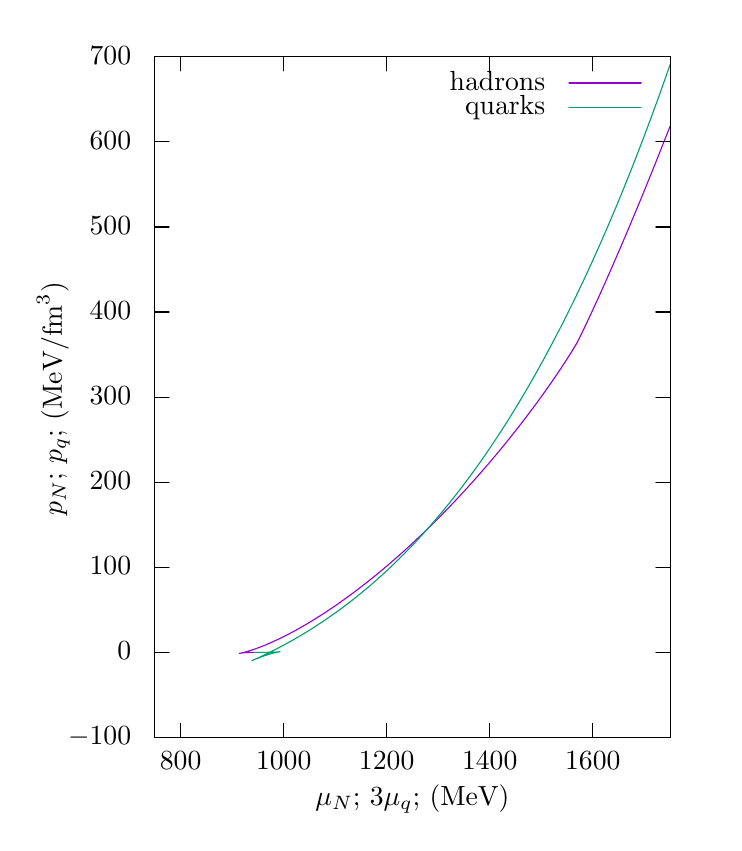
\begin{tikzpicture}[gnuplot]
%% generated with GNUPLOT 5.0p4 (Lua 5.2; terminal rev. 99, script rev. 100)
%% Thu Sep 29 16:33:17 2016
\path (0.000,0.000) rectangle (8.600,10.000);
\gpcolor{color=gp lt color border}
\gpsetlinetype{gp lt border}
\gpsetdashtype{gp dt solid}
\gpsetlinewidth{1.00}
\draw[gp path] (1.504,0.985)--(1.684,0.985);
\draw[gp path] (8.047,0.985)--(7.867,0.985);
\node[gp node right] at (1.320,0.985) {$-100$};
\draw[gp path] (1.504,2.066)--(1.684,2.066);
\draw[gp path] (8.047,2.066)--(7.867,2.066);
\node[gp node right] at (1.320,2.066) {$0$};
\draw[gp path] (1.504,3.147)--(1.684,3.147);
\draw[gp path] (8.047,3.147)--(7.867,3.147);
\node[gp node right] at (1.320,3.147) {$100$};
\draw[gp path] (1.504,4.227)--(1.684,4.227);
\draw[gp path] (8.047,4.227)--(7.867,4.227);
\node[gp node right] at (1.320,4.227) {$200$};
\draw[gp path] (1.504,5.308)--(1.684,5.308);
\draw[gp path] (8.047,5.308)--(7.867,5.308);
\node[gp node right] at (1.320,5.308) {$300$};
\draw[gp path] (1.504,6.389)--(1.684,6.389);
\draw[gp path] (8.047,6.389)--(7.867,6.389);
\node[gp node right] at (1.320,6.389) {$400$};
\draw[gp path] (1.504,7.469)--(1.684,7.469);
\draw[gp path] (8.047,7.469)--(7.867,7.469);
\node[gp node right] at (1.320,7.469) {$500$};
\draw[gp path] (1.504,8.550)--(1.684,8.550);
\draw[gp path] (8.047,8.550)--(7.867,8.550);
\node[gp node right] at (1.320,8.550) {$600$};
\draw[gp path] (1.504,9.631)--(1.684,9.631);
\draw[gp path] (8.047,9.631)--(7.867,9.631);
\node[gp node right] at (1.320,9.631) {$700$};
\draw[gp path] (1.831,0.985)--(1.831,1.165);
\draw[gp path] (1.831,9.631)--(1.831,9.451);
\node[gp node center] at (1.831,0.677) {$800$};
\draw[gp path] (3.140,0.985)--(3.140,1.165);
\draw[gp path] (3.140,9.631)--(3.140,9.451);
\node[gp node center] at (3.140,0.677) {$1000$};
\draw[gp path] (4.448,0.985)--(4.448,1.165);
\draw[gp path] (4.448,9.631)--(4.448,9.451);
\node[gp node center] at (4.448,0.677) {$1200$};
\draw[gp path] (5.757,0.985)--(5.757,1.165);
\draw[gp path] (5.757,9.631)--(5.757,9.451);
\node[gp node center] at (5.757,0.677) {$1400$};
\draw[gp path] (7.066,0.985)--(7.066,1.165);
\draw[gp path] (7.066,9.631)--(7.066,9.451);
\node[gp node center] at (7.066,0.677) {$1600$};
\draw[gp path] (1.504,9.631)--(1.504,0.985)--(8.047,0.985)--(8.047,9.631)--cycle;
\node[gp node center,rotate=-270] at (0.246,5.308) {$p_N$; $p_q$; ($\rm{MeV}/\rm{fm}^3$)};
\node[gp node center] at (4.775,0.215) {$\mu_N$; $3\mu_q$; (MeV)};
\node[gp node right] at (6.579,9.297) {hadrons};
\gpcolor{rgb color={0.580,0.000,0.827}}
\draw[gp path] (6.763,9.297)--(7.679,9.297);
\draw[gp path] (2.756,2.066)--(2.757,2.066)--(2.759,2.066)--(2.760,2.066)--(2.722,2.066)%
  --(2.723,2.066)--(2.724,2.066)--(2.725,2.066)--(2.726,2.066)--(2.727,2.066)--(2.728,2.066)%
  --(2.690,2.065)--(2.691,2.065)--(2.692,2.065)--(2.655,2.063)--(2.656,2.063)--(2.657,2.063)%
  --(2.658,2.063)--(2.659,2.063)--(2.622,2.060)--(2.623,2.060)--(2.624,2.060)--(2.625,2.060)%
  --(2.626,2.060)--(2.627,2.060)--(2.628,2.061)--(2.629,2.061)--(2.630,2.061)--(2.631,2.061)%
  --(2.632,2.061)--(2.595,2.057)--(2.596,2.057)--(2.597,2.057)--(2.598,2.057)--(2.599,2.057)%
  --(2.600,2.057)--(2.600,2.058)--(2.601,2.058)--(2.602,2.058)--(2.603,2.058)--(2.604,2.058)%
  --(2.605,2.058)--(2.606,2.058)--(2.607,2.058)--(2.608,2.058)--(2.608,2.059)--(2.609,2.059)%
  --(2.610,2.059)--(2.611,2.059)--(2.612,2.059)--(2.613,2.059)--(2.614,2.059)--(2.579,2.054)%
  --(2.580,2.055)--(2.581,2.055)--(2.582,2.055)--(2.583,2.055)--(2.584,2.055)--(2.585,2.055)%
  --(2.586,2.055)--(2.587,2.055)--(2.588,2.056)--(2.589,2.056)--(2.590,2.056)--(2.591,2.056)%
  --(2.592,2.056)--(2.593,2.056)--(2.594,2.057)--(2.595,2.057)--(2.596,2.057)--(2.597,2.057)%
  --(2.598,2.057)--(2.599,2.057)--(2.600,2.058)--(2.601,2.058)--(2.602,2.058)--(2.603,2.058)%
  --(2.604,2.058)--(2.605,2.058)--(2.606,2.059)--(2.607,2.059)--(2.608,2.059)--(2.609,2.059)%
  --(2.610,2.059)--(2.611,2.060)--(2.612,2.060)--(2.577,2.054)--(2.578,2.054)--(2.580,2.054)%
  --(2.581,2.054)--(2.582,2.054)--(2.583,2.055)--(2.584,2.055)--(2.585,2.055)--(2.586,2.055)%
  --(2.588,2.055)--(2.589,2.056)--(2.590,2.056)--(2.591,2.056)--(2.592,2.056)--(2.594,2.057)%
  --(2.595,2.057)--(2.596,2.057)--(2.597,2.057)--(2.599,2.058)--(2.600,2.058)--(2.601,2.058)%
  --(2.602,2.058)--(2.604,2.059)--(2.605,2.059)--(2.606,2.059)--(2.608,2.059)--(2.609,2.060)%
  --(2.610,2.060)--(2.612,2.060)--(2.613,2.061)--(2.614,2.061)--(2.616,2.061)--(2.617,2.061)%
  --(2.619,2.062)--(2.620,2.062)--(2.621,2.062)--(2.623,2.063)--(2.624,2.063)--(2.626,2.063)%
  --(2.627,2.064)--(2.628,2.064)--(2.630,2.064)--(2.631,2.065)--(2.633,2.065)--(2.599,2.057)%
  --(2.601,2.058)--(2.602,2.058)--(2.604,2.058)--(2.605,2.059)--(2.607,2.059)--(2.608,2.059)%
  --(2.610,2.060)--(2.611,2.060)--(2.613,2.061)--(2.615,2.061)--(2.616,2.061)--(2.618,2.062)%
  --(2.619,2.062)--(2.621,2.062)--(2.623,2.063)--(2.624,2.063)--(2.626,2.064)--(2.628,2.064)%
  --(2.629,2.064)--(2.631,2.065)--(2.633,2.065)--(2.634,2.066)--(2.636,2.066)--(2.638,2.067)%
  --(2.639,2.067)--(2.641,2.067)--(2.643,2.068)--(2.644,2.068)--(2.646,2.069)--(2.648,2.069)%
  --(2.650,2.070)--(2.652,2.070)--(2.653,2.071)--(2.655,2.071)--(2.657,2.072)--(2.659,2.072)%
  --(2.660,2.073)--(2.662,2.073)--(2.664,2.074)--(2.666,2.074)--(2.668,2.075)--(2.670,2.075)%
  --(2.671,2.076)--(2.673,2.076)--(2.675,2.077)--(2.677,2.077)--(2.679,2.078)--(2.681,2.079)%
  --(2.683,2.079)--(2.685,2.080)--(2.687,2.080)--(2.689,2.081)--(2.691,2.081)--(2.692,2.082)%
  --(2.694,2.083)--(2.696,2.083)--(2.698,2.084)--(2.700,2.084)--(2.702,2.085)--(2.704,2.086)%
  --(2.706,2.086)--(2.674,2.076)--(2.676,2.077)--(2.678,2.078)--(2.680,2.078)--(2.682,2.079)%
  --(2.684,2.079)--(2.686,2.080)--(2.688,2.081)--(2.690,2.081)--(2.692,2.082)--(2.695,2.083)%
  --(2.697,2.083)--(2.699,2.084)--(2.701,2.085)--(2.703,2.085)--(2.705,2.086)--(2.707,2.087)%
  --(2.709,2.087)--(2.712,2.088)--(2.714,2.089)--(2.716,2.089)--(2.718,2.090)--(2.720,2.091)%
  --(2.723,2.091)--(2.725,2.092)--(2.727,2.093)--(2.729,2.094)--(2.731,2.094)--(2.734,2.095)%
  --(2.736,2.096)--(2.738,2.097)--(2.741,2.097)--(2.743,2.098)--(2.745,2.099)--(2.747,2.100)%
  --(2.750,2.100)--(2.752,2.101)--(2.754,2.102)--(2.757,2.103)--(2.759,2.104)--(2.761,2.104)%
  --(2.764,2.105)--(2.766,2.106)--(2.768,2.107)--(2.771,2.108)--(2.773,2.108)--(2.776,2.109)%
  --(2.778,2.110)--(2.780,2.111)--(2.783,2.112)--(2.785,2.113)--(2.788,2.114)--(2.790,2.114)%
  --(2.792,2.115)--(2.795,2.116)--(2.797,2.117)--(2.800,2.118)--(2.802,2.119)--(2.805,2.120)%
  --(2.807,2.121)--(2.810,2.122)--(2.812,2.123)--(2.815,2.123)--(2.817,2.124)--(2.820,2.125)%
  --(2.822,2.126)--(2.825,2.127)--(2.827,2.128)--(2.830,2.129)--(2.833,2.130)--(2.835,2.131)%
  --(2.838,2.132)--(2.840,2.133)--(2.843,2.134)--(2.845,2.135)--(2.848,2.136)--(2.851,2.137)%
  --(2.853,2.138)--(2.856,2.139)--(2.859,2.140)--(2.861,2.141)--(2.864,2.142)--(2.866,2.143)%
  --(2.869,2.144)--(2.872,2.145)--(2.874,2.147)--(2.877,2.148)--(2.880,2.149)--(2.883,2.150)%
  --(2.885,2.151)--(2.888,2.152)--(2.891,2.153)--(2.893,2.154)--(2.896,2.155)--(2.899,2.156)%
  --(2.902,2.158)--(2.904,2.159)--(2.907,2.160)--(2.910,2.161)--(2.913,2.162)--(2.916,2.163)%
  --(2.918,2.164)--(2.921,2.166)--(2.924,2.167)--(2.927,2.168)--(2.930,2.169)--(2.932,2.170)%
  --(2.935,2.172)--(2.938,2.173)--(2.941,2.174)--(2.944,2.175)--(2.947,2.176)--(2.950,2.178)%
  --(2.952,2.179)--(2.955,2.180)--(2.958,2.181)--(2.961,2.183)--(2.931,2.170)--(2.933,2.171)%
  --(2.936,2.172)--(2.939,2.173)--(2.942,2.175)--(2.945,2.176)--(2.948,2.177)--(2.951,2.178)%
  --(2.954,2.180)--(2.957,2.181)--(2.960,2.182)--(2.963,2.184)--(2.966,2.185)--(2.969,2.186)%
  --(2.972,2.188)--(2.975,2.189)--(2.978,2.190)--(2.981,2.192)--(2.984,2.193)--(2.987,2.194)%
  --(2.990,2.196)--(2.993,2.197)--(2.996,2.198)--(3.000,2.200)--(3.003,2.201)--(3.006,2.203)%
  --(3.009,2.204)--(3.012,2.205)--(3.015,2.207)--(3.018,2.208)--(3.021,2.210)--(3.024,2.211)%
  --(3.027,2.212)--(3.031,2.214)--(3.034,2.215)--(3.037,2.217)--(3.040,2.218)--(3.043,2.220)%
  --(3.046,2.221)--(3.050,2.223)--(3.053,2.224)--(3.056,2.226)--(3.059,2.227)--(3.062,2.229)%
  --(3.066,2.230)--(3.069,2.232)--(3.072,2.233)--(3.075,2.235)--(3.079,2.236)--(3.082,2.238)%
  --(3.085,2.240)--(3.088,2.241)--(3.092,2.243)--(3.095,2.244)--(3.098,2.246)--(3.101,2.248)%
  --(3.105,2.249)--(3.108,2.251)--(3.111,2.252)--(3.115,2.254)--(3.118,2.256)--(3.121,2.257)%
  --(3.125,2.259)--(3.128,2.261)--(3.131,2.262)--(3.135,2.264)--(3.138,2.266)--(3.141,2.267)%
  --(3.145,2.269)--(3.148,2.271)--(3.151,2.272)--(3.155,2.274)--(3.158,2.276)--(3.162,2.277)%
  --(3.165,2.279)--(3.168,2.281)--(3.172,2.283)--(3.175,2.284)--(3.179,2.286)--(3.182,2.288)%
  --(3.186,2.290)--(3.189,2.291)--(3.192,2.293)--(3.196,2.295)--(3.199,2.297)--(3.203,2.299)%
  --(3.206,2.300)--(3.210,2.302)--(3.213,2.304)--(3.217,2.306)--(3.220,2.308)--(3.224,2.310)%
  --(3.227,2.312)--(3.231,2.313)--(3.234,2.315)--(3.238,2.317)--(3.241,2.319)--(3.245,2.321)%
  --(3.249,2.323)--(3.252,2.325)--(3.256,2.327)--(3.259,2.329)--(3.263,2.330)--(3.266,2.332)%
  --(3.270,2.334)--(3.274,2.336)--(3.277,2.338)--(3.281,2.340)--(3.284,2.342)--(3.288,2.344)%
  --(3.292,2.346)--(3.295,2.348)--(3.299,2.350)--(3.303,2.352)--(3.306,2.354)--(3.310,2.356)%
  --(3.314,2.358)--(3.317,2.360)--(3.321,2.362)--(3.325,2.364)--(3.328,2.366)--(3.332,2.368)%
  --(3.336,2.371)--(3.339,2.373)--(3.343,2.375)--(3.347,2.377)--(3.350,2.379)--(3.354,2.381)%
  --(3.358,2.383)--(3.362,2.385)--(3.365,2.387)--(3.369,2.390)--(3.373,2.392)--(3.377,2.394)%
  --(3.380,2.396)--(3.384,2.398)--(3.388,2.400)--(3.392,2.402)--(3.395,2.405)--(3.399,2.407)%
  --(3.403,2.409)--(3.407,2.411)--(3.411,2.414)--(3.414,2.416)--(3.418,2.418)--(3.422,2.420)%
  --(3.426,2.422)--(3.430,2.425)--(3.434,2.427)--(3.437,2.429)--(3.441,2.432)--(3.445,2.434)%
  --(3.449,2.436)--(3.453,2.438)--(3.457,2.441)--(3.461,2.443)--(3.464,2.445)--(3.468,2.448)%
  --(3.472,2.450)--(3.476,2.452)--(3.480,2.455)--(3.484,2.457)--(3.488,2.459)--(3.492,2.462)%
  --(3.496,2.464)--(3.500,2.467)--(3.504,2.469)--(3.508,2.471)--(3.511,2.474)--(3.515,2.476)%
  --(3.519,2.479)--(3.523,2.481)--(3.527,2.484)--(3.531,2.486)--(3.535,2.488)--(3.539,2.491)%
  --(3.543,2.493)--(3.547,2.496)--(3.551,2.498)--(3.555,2.501)--(3.559,2.503)--(3.563,2.506)%
  --(3.567,2.508)--(3.571,2.511)--(3.575,2.514)--(3.579,2.516)--(3.583,2.519)--(3.587,2.521)%
  --(3.591,2.524)--(3.596,2.526)--(3.600,2.529)--(3.604,2.531)--(3.608,2.534)--(3.612,2.537)%
  --(3.616,2.539)--(3.620,2.542)--(3.624,2.545)--(3.628,2.547)--(3.632,2.550)--(3.636,2.552)%
  --(3.640,2.555)--(3.645,2.558)--(3.649,2.560)--(3.653,2.563)--(3.657,2.566)--(3.661,2.569)%
  --(3.665,2.571)--(3.669,2.574)--(3.673,2.577)--(3.678,2.579)--(3.682,2.582)--(3.686,2.585)%
  --(3.690,2.588)--(3.694,2.590)--(3.698,2.593)--(3.703,2.596)--(3.707,2.599)--(3.711,2.602)%
  --(3.715,2.604)--(3.719,2.607)--(3.724,2.610)--(3.728,2.613)--(3.732,2.616)--(3.736,2.618)%
  --(3.740,2.621)--(3.745,2.624)--(3.749,2.627)--(3.753,2.630)--(3.757,2.633)--(3.762,2.636)%
  --(3.766,2.639)--(3.770,2.641)--(3.774,2.644)--(3.779,2.647)--(3.783,2.650)--(3.787,2.653)%
  --(3.792,2.656)--(3.796,2.659)--(3.800,2.662)--(3.804,2.665)--(3.809,2.668)--(3.813,2.671)%
  --(3.817,2.674)--(3.822,2.677)--(3.826,2.680)--(3.830,2.683)--(3.835,2.686)--(3.839,2.689)%
  --(3.843,2.692)--(3.848,2.695)--(3.852,2.698)--(3.856,2.701)--(3.861,2.704)--(3.865,2.707)%
  --(3.869,2.710)--(3.874,2.713)--(3.878,2.716)--(3.882,2.720)--(3.887,2.723)--(3.891,2.726)%
  --(3.896,2.729)--(3.900,2.732)--(3.904,2.735)--(3.909,2.738)--(3.913,2.742)--(3.918,2.745)%
  --(3.922,2.748)--(3.926,2.751)--(3.931,2.754)--(3.935,2.757)--(3.940,2.761)--(3.944,2.764)%
  --(3.949,2.767)--(3.953,2.770)--(3.957,2.774)--(3.962,2.777)--(3.966,2.780)--(3.971,2.783)%
  --(3.975,2.787)--(3.980,2.790)--(3.984,2.793)--(3.989,2.797)--(3.993,2.800)--(3.998,2.803)%
  --(4.002,2.806)--(4.007,2.810)--(4.011,2.813)--(4.016,2.816)--(4.020,2.820)--(4.025,2.823)%
  --(4.029,2.827)--(4.034,2.830)--(4.038,2.833)--(4.043,2.837)--(4.047,2.840)--(4.052,2.844)%
  --(4.056,2.847)--(4.061,2.850)--(4.065,2.854)--(4.070,2.857)--(4.074,2.861)--(4.079,2.864)%
  --(4.083,2.868)--(4.088,2.871)--(4.093,2.875)--(4.097,2.878)--(4.102,2.882)--(4.106,2.885)%
  --(4.111,2.889)--(4.115,2.892)--(4.120,2.896)--(4.125,2.899)--(4.129,2.903)--(4.134,2.906)%
  --(4.138,2.910)--(4.143,2.913)--(4.148,2.917)--(4.152,2.921)--(4.157,2.924)--(4.162,2.928)%
  --(4.166,2.931)--(4.171,2.935)--(4.175,2.939)--(4.180,2.942)--(4.185,2.946)--(4.189,2.950)%
  --(4.194,2.953)--(4.199,2.957)--(4.203,2.961)--(4.208,2.964)--(4.213,2.968)--(4.217,2.972)%
  --(4.222,2.975)--(4.227,2.979)--(4.231,2.983)--(4.236,2.987)--(4.241,2.990)--(4.245,2.994)%
  --(4.250,2.998)--(4.255,3.002)--(4.259,3.005)--(4.264,3.009)--(4.269,3.013)--(4.274,3.017)%
  --(4.278,3.020)--(4.283,3.024)--(4.288,3.028)--(4.292,3.032)--(4.297,3.036)--(4.302,3.040)%
  --(4.307,3.043)--(4.311,3.047)--(4.316,3.051)--(4.321,3.055)--(4.326,3.059)--(4.330,3.063)%
  --(4.335,3.067)--(4.340,3.071)--(4.345,3.075)--(4.349,3.079)--(4.354,3.082)--(4.359,3.086)%
  --(4.364,3.090)--(4.368,3.094)--(4.373,3.098)--(4.378,3.102)--(4.383,3.106)--(4.387,3.110)%
  --(4.392,3.114)--(4.397,3.118)--(4.402,3.122)--(4.407,3.126)--(4.411,3.130)--(4.416,3.134)%
  --(4.421,3.138)--(4.426,3.143)--(4.431,3.147)--(4.436,3.151)--(4.440,3.155)--(4.445,3.159)%
  --(4.450,3.163)--(4.455,3.167)--(4.460,3.171)--(4.464,3.175)--(4.469,3.179)--(4.474,3.184)%
  --(4.479,3.188)--(4.484,3.192)--(4.489,3.196)--(4.494,3.200)--(4.498,3.204)--(4.503,3.209)%
  --(4.508,3.213)--(4.513,3.217)--(4.518,3.221)--(4.523,3.225)--(4.528,3.230)--(4.533,3.234)%
  --(4.537,3.238)--(4.542,3.242)--(4.547,3.247)--(4.552,3.251)--(4.557,3.255)--(4.562,3.259)%
  --(4.567,3.264)--(4.572,3.268)--(4.577,3.272)--(4.581,3.277)--(4.586,3.281)--(4.591,3.285)%
  --(4.596,3.290)--(4.601,3.294)--(4.606,3.298)--(4.611,3.303)--(4.616,3.307)--(4.621,3.312)%
  --(4.626,3.316)--(4.598,3.292)--(4.603,3.296)--(4.608,3.300)--(4.613,3.305)--(4.618,3.309)%
  --(4.623,3.314)--(4.628,3.318)--(4.633,3.323)--(4.638,3.327)--(4.643,3.331)--(4.648,3.336)%
  --(4.653,3.340)--(4.658,3.345)--(4.663,3.349)--(4.668,3.354)--(4.673,3.358)--(4.678,3.363)%
  --(4.683,3.367)--(4.688,3.372)--(4.693,3.376)--(4.698,3.381)--(4.703,3.385)--(4.708,3.390)%
  --(4.713,3.394)--(4.718,3.399)--(4.723,3.404)--(4.728,3.408)--(4.733,3.413)--(4.738,3.417)%
  --(4.743,3.422)--(4.748,3.427)--(4.753,3.431)--(4.758,3.436)--(4.763,3.440)--(4.768,3.445)%
  --(4.773,3.450)--(4.778,3.454)--(4.783,3.459)--(4.788,3.464)--(4.793,3.468)--(4.798,3.473)%
  --(4.803,3.478)--(4.808,3.483)--(4.813,3.487)--(4.818,3.492)--(4.823,3.497)--(4.828,3.501)%
  --(4.833,3.506)--(4.838,3.511)--(4.843,3.516)--(4.848,3.520)--(4.853,3.525)--(4.859,3.530)%
  --(4.864,3.535)--(4.869,3.540)--(4.874,3.544)--(4.879,3.549)--(4.884,3.554)--(4.889,3.559)%
  --(4.894,3.564)--(4.899,3.569)--(4.904,3.574)--(4.909,3.578)--(4.914,3.583)--(4.919,3.588)%
  --(4.925,3.593)--(4.930,3.598)--(4.935,3.603)--(4.940,3.608)--(4.945,3.613)--(4.950,3.618)%
  --(4.955,3.623)--(4.960,3.628)--(4.965,3.633)--(4.970,3.637)--(4.976,3.642)--(4.981,3.647)%
  --(4.954,3.621)--(4.959,3.626)--(4.964,3.631)--(4.969,3.636)--(4.974,3.641)--(4.979,3.646)%
  --(4.984,3.651)--(4.989,3.656)--(4.995,3.661)--(5.000,3.666)--(5.005,3.671)--(5.010,3.676)%
  --(5.015,3.681)--(5.020,3.686)--(5.025,3.691)--(5.031,3.696)--(5.036,3.702)--(5.041,3.707)%
  --(5.046,3.712)--(5.051,3.717)--(5.056,3.722)--(5.061,3.727)--(5.067,3.732)--(5.072,3.737)%
  --(5.077,3.743)--(5.082,3.748)--(5.087,3.753)--(5.092,3.758)--(5.097,3.763)--(5.103,3.768)%
  --(5.108,3.774)--(5.113,3.779)--(5.118,3.784)--(5.123,3.789)--(5.128,3.794)--(5.134,3.800)%
  --(5.139,3.805)--(5.144,3.810)--(5.149,3.815)--(5.154,3.821)--(5.160,3.826)--(5.165,3.831)%
  --(5.170,3.837)--(5.175,3.842)--(5.180,3.847)--(5.185,3.853)--(5.191,3.858)--(5.196,3.863)%
  --(5.201,3.869)--(5.206,3.874)--(5.211,3.879)--(5.217,3.885)--(5.190,3.857)--(5.195,3.862)%
  --(5.200,3.868)--(5.205,3.873)--(5.210,3.878)--(5.216,3.884)--(5.221,3.889)--(5.226,3.894)%
  --(5.231,3.900)--(5.236,3.905)--(5.242,3.911)--(5.247,3.916)--(5.252,3.922)--(5.257,3.927)%
  --(5.263,3.932)--(5.268,3.938)--(5.273,3.943)--(5.278,3.949)--(5.283,3.954)--(5.289,3.960)%
  --(5.294,3.965)--(5.299,3.971)--(5.304,3.976)--(5.310,3.982)--(5.315,3.987)--(5.320,3.993)%
  --(5.325,3.998)--(5.330,4.004)--(5.336,4.010)--(5.341,4.015)--(5.346,4.021)--(5.351,4.026)%
  --(5.357,4.032)--(5.362,4.037)--(5.367,4.043)--(5.372,4.049)--(5.378,4.054)--(5.383,4.060)%
  --(5.388,4.066)--(5.393,4.071)--(5.366,4.042)--(5.372,4.048)--(5.377,4.054)--(5.382,4.059)%
  --(5.387,4.065)--(5.393,4.071)--(5.398,4.076)--(5.403,4.082)--(5.408,4.088)--(5.414,4.093)%
  --(5.419,4.099)--(5.424,4.105)--(5.429,4.110)--(5.435,4.116)--(5.440,4.122)--(5.445,4.127)%
  --(5.450,4.133)--(5.456,4.139)--(5.461,4.145)--(5.466,4.150)--(5.471,4.156)--(5.477,4.162)%
  --(5.482,4.168)--(5.487,4.174)--(5.493,4.179)--(5.498,4.185)--(5.503,4.191)--(5.508,4.197)%
  --(5.514,4.203)--(5.519,4.209)--(5.524,4.214)--(5.529,4.220)--(5.535,4.226)--(5.540,4.232)%
  --(5.513,4.202)--(5.518,4.208)--(5.524,4.214)--(5.529,4.220)--(5.534,4.226)--(5.539,4.231)%
  --(5.545,4.237)--(5.550,4.243)--(5.555,4.249)--(5.561,4.255)--(5.566,4.261)--(5.571,4.267)%
  --(5.576,4.273)--(5.582,4.279)--(5.587,4.285)--(5.592,4.291)--(5.598,4.297)--(5.603,4.303)%
  --(5.608,4.309)--(5.613,4.315)--(5.619,4.321)--(5.624,4.327)--(5.629,4.333)--(5.634,4.339)%
  --(5.640,4.345)--(5.645,4.351)--(5.650,4.357)--(5.656,4.363)--(5.661,4.369)--(5.634,4.338)%
  --(5.639,4.344)--(5.645,4.350)--(5.650,4.356)--(5.655,4.362)--(5.661,4.368)--(5.666,4.374)%
  --(5.671,4.381)--(5.676,4.387)--(5.682,4.393)--(5.687,4.399)--(5.692,4.405)--(5.698,4.411)%
  --(5.703,4.417)--(5.708,4.423)--(5.713,4.429)--(5.719,4.436)--(5.724,4.442)--(5.729,4.448)%
  --(5.735,4.454)--(5.740,4.460)--(5.745,4.466)--(5.750,4.473)--(5.756,4.479)--(5.761,4.485)%
  --(5.766,4.491)--(5.739,4.460)--(5.745,4.466)--(5.750,4.472)--(5.755,4.478)--(5.761,4.485)%
  --(5.766,4.491)--(5.771,4.497)--(5.776,4.503)--(5.782,4.510)--(5.787,4.516)--(5.792,4.522)%
  --(5.798,4.528)--(5.803,4.535)--(5.808,4.541)--(5.813,4.547)--(5.819,4.553)--(5.824,4.560)%
  --(5.829,4.566)--(5.835,4.572)--(5.840,4.579)--(5.845,4.585)--(5.851,4.591)--(5.856,4.598)%
  --(5.861,4.604)--(5.834,4.572)--(5.840,4.578)--(5.845,4.585)--(5.850,4.591)--(5.855,4.597)%
  --(5.861,4.604)--(5.866,4.610)--(5.871,4.616)--(5.877,4.623)--(5.882,4.629)--(5.887,4.636)%
  --(5.892,4.642)--(5.898,4.648)--(5.903,4.655)--(5.908,4.661)--(5.914,4.668)--(5.919,4.674)%
  --(5.924,4.681)--(5.929,4.687)--(5.935,4.693)--(5.940,4.700)--(5.945,4.706)--(5.919,4.674)%
  --(5.924,4.680)--(5.929,4.687)--(5.934,4.693)--(5.940,4.699)--(5.945,4.706)--(5.950,4.712)%
  --(5.955,4.719)--(5.961,4.725)--(5.966,4.732)--(5.971,4.738)--(5.977,4.745)--(5.982,4.751)%
  --(5.987,4.758)--(5.992,4.765)--(5.998,4.771)--(6.003,4.778)--(6.008,4.784)--(6.013,4.791)%
  --(6.019,4.797)--(5.992,4.764)--(5.997,4.771)--(6.003,4.777)--(6.008,4.784)--(6.013,4.790)%
  --(6.018,4.797)--(6.024,4.803)--(6.029,4.810)--(6.034,4.817)--(6.039,4.823)--(6.045,4.830)%
  --(6.050,4.836)--(6.055,4.843)--(6.060,4.850)--(6.066,4.856)--(6.071,4.863)--(6.076,4.870)%
  --(6.082,4.876)--(6.087,4.883)--(6.060,4.849)--(6.065,4.856)--(6.071,4.862)--(6.076,4.869)%
  --(6.081,4.876)--(6.086,4.882)--(6.092,4.889)--(6.097,4.896)--(6.102,4.903)--(6.107,4.909)%
  --(6.113,4.916)--(6.118,4.923)--(6.123,4.929)--(6.128,4.936)--(6.134,4.943)--(6.139,4.950)%
  --(6.144,4.956)--(6.149,4.963)--(6.123,4.929)--(6.128,4.935)--(6.133,4.942)--(6.138,4.949)%
  --(6.144,4.956)--(6.149,4.962)--(6.154,4.969)--(6.159,4.976)--(6.164,4.983)--(6.170,4.989)%
  --(6.175,4.996)--(6.180,5.003)--(6.185,5.010)--(6.191,5.017)--(6.196,5.023)--(6.201,5.030)%
  --(6.174,4.996)--(6.180,5.002)--(6.185,5.009)--(6.190,5.016)--(6.195,5.023)--(6.200,5.030)%
  --(6.206,5.036)--(6.211,5.043)--(6.216,5.050)--(6.221,5.057)--(6.227,5.064)--(6.232,5.071)%
  --(6.237,5.077)--(6.242,5.084)--(6.247,5.091)--(6.253,5.098)--(6.258,5.105)--(6.231,5.070)%
  --(6.236,5.077)--(6.241,5.083)--(6.247,5.090)--(6.252,5.097)--(6.257,5.104)--(6.262,5.111)%
  --(6.267,5.118)--(6.273,5.125)--(6.278,5.132)--(6.283,5.139)--(6.288,5.146)--(6.293,5.153)%
  --(6.299,5.159)--(6.304,5.166)--(6.277,5.131)--(6.282,5.138)--(6.287,5.145)--(6.293,5.152)%
  --(6.298,5.158)--(6.303,5.165)--(6.308,5.172)--(6.313,5.179)--(6.318,5.186)--(6.324,5.193)%
  --(6.329,5.200)--(6.334,5.207)--(6.339,5.214)--(6.344,5.221)--(6.318,5.185)--(6.323,5.192)%
  --(6.328,5.199)--(6.333,5.206)--(6.338,5.213)--(6.343,5.220)--(6.349,5.227)--(6.354,5.234)%
  --(6.359,5.241)--(6.364,5.248)--(6.369,5.255)--(6.374,5.262)--(6.379,5.269)--(6.385,5.276)%
  --(6.390,5.283)--(6.363,5.247)--(6.368,5.254)--(6.373,5.261)--(6.379,5.268)--(6.384,5.275)%
  --(6.389,5.282)--(6.394,5.289)--(6.399,5.296)--(6.404,5.303)--(6.409,5.310)--(6.414,5.317)%
  --(6.419,5.325)--(6.425,5.332)--(6.398,5.295)--(6.403,5.302)--(6.408,5.309)--(6.413,5.316)%
  --(6.418,5.323)--(6.424,5.330)--(6.429,5.337)--(6.434,5.344)--(6.439,5.351)--(6.444,5.359)%
  --(6.449,5.366)--(6.454,5.373)--(6.459,5.380)--(6.433,5.343)--(6.438,5.350)--(6.443,5.357)%
  --(6.448,5.364)--(6.453,5.371)--(6.458,5.378)--(6.463,5.385)--(6.468,5.393)--(6.473,5.400)%
  --(6.478,5.407)--(6.483,5.414)--(6.488,5.421)--(6.493,5.428)--(6.467,5.391)--(6.472,5.398)%
  --(6.477,5.405)--(6.482,5.412)--(6.487,5.419)--(6.492,5.427)--(6.497,5.434)--(6.502,5.441)%
  --(6.507,5.448)--(6.512,5.455)--(6.517,5.462)--(6.522,5.470)--(6.496,5.432)--(6.501,5.439)%
  --(6.506,5.446)--(6.511,5.453)--(6.516,5.461)--(6.521,5.468)--(6.526,5.475)--(6.531,5.482)%
  --(6.536,5.489)--(6.541,5.497)--(6.546,5.504)--(6.551,5.511)--(6.525,5.473)--(6.530,5.480)%
  --(6.535,5.487)--(6.540,5.494)--(6.545,5.502)--(6.550,5.509)--(6.555,5.516)--(6.560,5.523)%
  --(6.565,5.531)--(6.570,5.538)--(6.575,5.545)--(6.548,5.507)--(6.553,5.514)--(6.558,5.521)%
  --(6.563,5.528)--(6.568,5.535)--(6.573,5.543)--(6.578,5.550)--(6.583,5.557)--(6.588,5.564)%
  --(6.593,5.572)--(6.598,5.579)--(6.603,5.586)--(6.576,5.547)--(6.581,5.555)--(6.586,5.562)%
  --(6.591,5.569)--(6.596,5.576)--(6.601,5.584)--(6.606,5.591)--(6.611,5.598)--(6.616,5.606)%
  --(6.621,5.613)--(6.626,5.620)--(6.599,5.581)--(6.604,5.588)--(6.609,5.596)--(6.614,5.603)%
  --(6.619,5.610)--(6.624,5.617)--(6.629,5.625)--(6.634,5.632)--(6.639,5.639)--(6.643,5.647)%
  --(6.617,5.607)--(6.622,5.615)--(6.627,5.622)--(6.632,5.629)--(6.637,5.636)--(6.641,5.644)%
  --(6.646,5.651)--(6.651,5.658)--(6.656,5.666)--(6.661,5.673)--(6.666,5.680)--(6.639,5.641)%
  --(6.644,5.648)--(6.649,5.655)--(6.654,5.663)--(6.659,5.670)--(6.664,5.677)--(6.669,5.685)%
  --(6.673,5.692)--(6.678,5.699)--(6.683,5.707)--(6.657,5.667)--(6.662,5.674)--(6.666,5.681)%
  --(6.671,5.689)--(6.676,5.696)--(6.681,5.703)--(6.686,5.711)--(6.691,5.718)--(6.695,5.725)%
  --(6.700,5.733)--(6.674,5.693)--(6.679,5.700)--(6.684,5.707)--(6.688,5.715)--(6.693,5.722)%
  --(6.698,5.729)--(6.703,5.737)--(6.708,5.744)--(6.712,5.751)--(6.717,5.759)--(6.691,5.718)%
  --(6.696,5.726)--(6.700,5.733)--(6.705,5.740)--(6.710,5.748)--(6.715,5.755)--(6.719,5.762)%
  --(6.724,5.770)--(6.729,5.777)--(6.703,5.736)--(6.708,5.744)--(6.712,5.751)--(6.717,5.758)%
  --(6.722,5.766)--(6.727,5.773)--(6.731,5.781)--(6.736,5.788)--(6.741,5.795)--(6.745,5.803)%
  --(6.719,5.762)--(6.724,5.769)--(6.729,5.777)--(6.733,5.784)--(6.738,5.791)--(6.743,5.799)%
  --(6.748,5.806)--(6.752,5.813)--(6.757,5.821)--(6.731,5.780)--(6.735,5.787)--(6.740,5.794)%
  --(6.745,5.802)--(6.750,5.809)--(6.754,5.816)--(6.759,5.824)--(6.764,5.831)--(6.768,5.839)%
  --(6.742,5.797)--(6.747,5.805)--(6.751,5.812)--(6.756,5.819)--(6.761,5.827)--(6.765,5.834)%
  --(6.770,5.842)--(6.775,5.849)--(6.779,5.856)--(6.753,5.815)--(6.758,5.822)--(6.763,5.830)%
  --(6.767,5.837)--(6.772,5.844)--(6.776,5.852)--(6.781,5.859)--(6.786,5.866)--(6.790,5.874)%
  --(6.764,5.832)--(6.769,5.840)--(6.774,5.847)--(6.778,5.854)--(6.783,5.862)--(6.787,5.869)%
  --(6.792,5.876)--(6.797,5.884)--(6.801,5.891)--(6.775,5.849)--(6.780,5.857)--(6.784,5.864)%
  --(6.789,5.871)--(6.793,5.879)--(6.798,5.886)--(6.803,5.894)--(6.807,5.901)--(6.781,5.859)%
  --(6.786,5.866)--(6.790,5.874)--(6.795,5.881)--(6.799,5.888)--(6.804,5.896)--(6.808,5.903)%
  --(6.813,5.911)--(6.818,5.918)--(6.792,5.876)--(6.796,5.883)--(6.801,5.891)--(6.805,5.898)%
  --(6.810,5.905)--(6.814,5.913)--(6.819,5.920)--(6.823,5.927)--(6.797,5.885)--(6.802,5.892)%
  --(6.806,5.900)--(6.811,5.907)--(6.815,5.914)--(6.820,5.922)--(6.824,5.929)--(6.829,5.937)%
  --(6.803,5.894)--(6.808,5.902)--(6.812,5.909)--(6.816,5.916)--(6.821,5.924)--(6.825,5.931)%
  --(6.830,5.938)--(6.834,5.946)--(6.809,5.903)--(6.813,5.911)--(6.817,5.918)--(6.822,5.925)%
  --(6.826,5.933)--(6.831,5.940)--(6.835,5.947)--(6.840,5.955)--(6.814,5.912)--(6.818,5.919)%
  --(6.823,5.927)--(6.827,5.934)--(6.832,5.941)--(6.836,5.949)--(6.840,5.956)--(6.845,5.963)%
  --(6.819,5.921)--(6.824,5.928)--(6.828,5.935)--(6.832,5.943)--(6.837,5.950)--(6.841,5.957)%
  --(6.845,5.964)--(6.850,5.972)--(6.824,5.929)--(6.829,5.936)--(6.833,5.944)--(6.837,5.951)%
  --(6.842,5.958)--(6.846,5.966)--(6.850,5.973)--(6.855,5.980)--(6.829,5.937)--(6.834,5.945)%
  --(6.838,5.952)--(6.842,5.959)--(6.847,5.967)--(6.851,5.974)--(6.855,5.981)--(6.860,5.988)%
  --(6.834,5.946)--(6.839,5.953)--(6.843,5.960)--(6.847,5.967)--(6.851,5.975)--(6.856,5.982)%
  --(6.860,5.989)--(6.835,5.946)--(6.839,5.953)--(6.843,5.961)--(6.848,5.968)--(6.852,5.975)%
  --(6.856,5.983)--(6.860,5.990)--(6.865,5.997)--(6.839,5.954)--(6.844,5.961)--(6.848,5.969)%
  --(6.852,5.976)--(6.856,5.983)--(6.861,5.990)--(6.865,5.998)--(6.840,5.955)--(6.844,5.962)%
  --(6.848,5.969)--(6.852,5.976)--(6.857,5.984)--(6.861,5.991)--(6.865,5.998)--(6.869,6.005)%
  --(6.851,5.975)--(6.856,5.982)--(6.860,5.989)--(6.864,5.996)--(6.854,5.978)--(6.858,5.986)%
  --(6.862,5.993)--(6.852,5.975)--(6.856,5.982)--(6.860,5.989)--(6.864,5.997)--(6.854,5.979)%
  --(6.858,5.986)--(6.862,5.993)--(6.866,6.000)--(6.856,5.982)--(6.860,5.989)--(6.864,5.997)%
  --(6.854,5.979)--(6.858,5.986)--(6.862,5.993)--(6.866,6.000)--(6.856,5.982)--(6.860,5.990)%
  --(6.864,5.997)--(6.868,6.004)--(6.858,5.986)--(6.862,5.993)--(6.866,6.000)--(6.856,5.982)%
  --(6.860,5.989)--(6.864,5.997)--(6.868,6.004)--(6.858,5.986)--(6.862,5.993)--(6.866,6.000)%
  --(6.870,6.007)--(6.860,5.989)--(6.864,5.996)--(6.868,6.004)--(6.858,5.986)--(6.862,5.993)%
  --(6.866,6.000)--(6.870,6.007)--(6.860,5.989)--(6.864,5.996)--(6.868,6.003)--(6.858,5.985)%
  --(6.862,5.992)--(6.866,6.000)--(6.870,6.007)--(6.860,5.989)--(6.864,5.996)--(6.868,6.003)%
  --(6.858,5.985)--(6.862,5.992)--(6.866,5.999)--(6.870,6.006)--(6.859,5.988)--(6.863,5.996)%
  --(6.867,6.003)--(6.871,6.010)--(6.861,5.992)--(6.865,5.999)--(6.869,6.006)--(6.859,5.988)%
  --(6.863,5.995)--(6.867,6.002)--(6.871,6.009)--(6.861,5.991)--(6.865,5.998)--(6.869,6.006)%
  --(6.859,5.988)--(6.863,5.995)--(6.867,6.002)--(6.871,6.009)--(6.861,5.991)--(6.865,5.998)%
  --(6.869,6.005)--(6.859,5.987)--(6.863,5.994)--(6.867,6.001)--(6.871,6.008)--(6.861,5.990)%
  --(6.865,5.998)--(6.869,6.005)--(6.859,5.987)--(6.863,5.994)--(6.866,6.001)--(6.870,6.008)%
  --(6.860,5.990)--(6.864,5.997)--(6.868,6.004)--(6.858,5.986)--(6.862,5.993)--(6.866,6.000)%
  --(6.870,6.007)--(6.860,5.990)--(6.864,5.997)--(6.868,6.004)--(6.858,5.986)--(6.862,5.993)%
  --(6.866,6.000)--(6.870,6.007)--(6.860,5.989)--(6.864,5.996)--(6.868,6.003)--(6.872,6.010)%
  --(6.862,5.992)--(6.866,5.999)--(6.869,6.007)--(6.860,5.989)--(6.864,5.996)--(6.867,6.003)%
  --(6.871,6.010)--(6.862,5.992)--(6.865,5.999)--(6.869,6.006)--(6.860,5.988)--(6.863,5.995)%
  --(6.867,6.002)--(6.871,6.009)--(6.861,5.992)--(6.865,5.999)--(6.869,6.006)--(6.860,5.988)%
  --(6.863,5.995)--(6.867,6.002)--(6.871,6.009)--(6.861,5.991)--(6.865,5.998)--(6.869,6.005)%
  --(6.859,5.988)--(6.863,5.995)--(6.867,6.002)--(6.871,6.009)--(6.861,5.991)--(6.865,5.998)%
  --(6.869,6.005)--(6.859,5.988)--(6.863,5.995)--(6.867,6.002)--(6.871,6.009)--(6.861,5.991)%
  --(6.865,5.998)--(6.869,6.005)--(6.859,5.988)--(6.863,5.995)--(6.867,6.002)--(6.871,6.009)%
  --(6.861,5.991)--(6.865,5.998)--(6.869,6.005)--(6.859,5.988)--(6.863,5.995)--(6.867,6.002)%
  --(6.871,6.009)--(6.861,5.991)--(6.865,5.998)--(6.869,6.005)--(6.872,6.012)--(6.863,5.995)%
  --(6.867,6.002)--(6.871,6.009)--(6.862,5.992)--(6.865,5.999)--(6.869,6.006)--(6.873,6.013)%
  --(6.864,5.995)--(6.867,6.002)--(6.871,6.009)--(6.862,5.992)--(6.866,5.999)--(6.869,6.006)%
  --(6.873,6.013)--(6.864,5.996)--(6.867,6.003)--(6.871,6.010)--(6.862,5.993)--(6.866,6.000)%
  --(6.869,6.007)--(6.873,6.014)--(6.864,5.997)--(6.868,6.004)--(6.872,6.011)--(6.875,6.018)%
  --(6.866,6.001)--(6.870,6.008)--(6.874,6.015)--(6.865,5.998)--(6.868,6.005)--(6.872,6.012)%
  --(6.876,6.019)--(6.867,6.002)--(6.871,6.009)--(6.874,6.016)--(6.878,6.023)--(6.869,6.006)%
  --(6.873,6.013)--(6.876,6.020)--(6.868,6.003)--(6.871,6.010)--(6.875,6.017)--(6.878,6.024)%
  --(6.870,6.008)--(6.873,6.015)--(6.877,6.021)--(6.881,6.028)--(6.872,6.012)--(6.876,6.019)%
  --(6.879,6.026)--(6.871,6.009)--(6.874,6.016)--(6.878,6.023)--(6.881,6.030)--(6.873,6.014)%
  --(6.877,6.021)--(6.880,6.028)--(6.884,6.035)--(6.875,6.018)--(6.879,6.025)--(6.882,6.032)%
  --(6.886,6.039)--(6.878,6.023)--(6.881,6.030)--(6.885,6.037)--(6.877,6.021)--(6.880,6.028)%
  --(6.884,6.035)--(6.887,6.042)--(6.879,6.026)--(6.883,6.033)--(6.886,6.040)--(6.890,6.046)%
  --(6.882,6.031)--(6.885,6.038)--(6.889,6.044)--(6.892,6.051)--(6.884,6.036)--(6.888,6.043)%
  --(6.891,6.049)--(6.883,6.034)--(6.887,6.041)--(6.890,6.048)--(6.894,6.055)--(6.886,6.039)%
  --(6.889,6.046)--(6.893,6.053)--(6.896,6.060)--(6.889,6.044)--(6.892,6.051)--(6.895,6.058)%
  --(6.899,6.065)--(6.891,6.050)--(6.895,6.057)--(6.898,6.064)--(6.902,6.071)--(6.894,6.055)%
  --(6.898,6.062)--(6.901,6.069)--(6.904,6.076)--(6.897,6.061)--(6.900,6.068)--(6.904,6.075)%
  --(6.907,6.082)--(6.900,6.067)--(6.903,6.074)--(6.907,6.081)--(6.910,6.088)--(6.903,6.073)%
  --(6.906,6.080)--(6.910,6.087)--(6.913,6.093)--(6.906,6.079)--(6.909,6.086)--(6.913,6.093)%
  --(6.916,6.099)--(6.909,6.085)--(6.912,6.092)--(6.916,6.099)--(6.919,6.106)--(6.912,6.091)%
  --(6.915,6.098)--(6.919,6.105)--(6.922,6.112)--(6.915,6.098)--(6.918,6.105)--(6.922,6.112)%
  --(6.925,6.118)--(6.918,6.104)--(6.922,6.111)--(6.925,6.118)--(6.928,6.125)--(6.922,6.111)%
  --(6.925,6.118)--(6.928,6.125)--(6.932,6.132)--(6.925,6.118)--(6.928,6.125)--(6.932,6.132)%
  --(6.935,6.139)--(6.938,6.146)--(6.932,6.132)--(6.935,6.139)--(6.939,6.146)--(6.942,6.153)%
  --(6.935,6.139)--(6.939,6.146)--(6.942,6.153)--(6.945,6.160)--(6.939,6.147)--(6.942,6.154)%
  --(6.946,6.161)--(6.949,6.167)--(6.952,6.174)--(6.946,6.161)--(6.949,6.168)--(6.953,6.175)%
  --(6.956,6.182)--(6.950,6.169)--(6.953,6.176)--(6.956,6.183)--(6.960,6.190)--(6.954,6.177)%
  --(6.957,6.184)--(6.960,6.191)--(6.964,6.198)--(6.967,6.205)--(6.961,6.192)--(6.964,6.199)%
  --(6.967,6.206)--(6.971,6.213)--(6.965,6.200)--(6.968,6.207)--(6.971,6.214)--(6.975,6.221)%
  --(6.978,6.228)--(6.972,6.216)--(6.976,6.223)--(6.979,6.230)--(6.982,6.237)--(6.976,6.225)%
  --(6.980,6.232)--(6.983,6.239)--(6.986,6.246)--(6.990,6.253)--(6.984,6.241)--(6.987,6.248)%
  --(6.991,6.255)--(6.994,6.262)--(6.988,6.250)--(6.992,6.257)--(6.995,6.264)--(6.998,6.271)%
  --(7.002,6.278)--(6.996,6.266)--(6.999,6.273)--(7.003,6.280)--(7.006,6.287)--(7.009,6.294)%
  --(7.004,6.283)--(7.007,6.290)--(7.011,6.297)--(7.014,6.304)--(7.009,6.293)--(7.012,6.300)%
  --(7.015,6.307)--(7.019,6.314)--(7.022,6.321)--(7.017,6.310)--(7.020,6.317)--(7.023,6.324)%
  --(7.027,6.331)--(7.030,6.338)--(7.025,6.327)--(7.028,6.334)--(7.031,6.341)--(7.035,6.349)%
  --(7.038,6.356)--(7.033,6.345)--(7.036,6.352)--(7.040,6.359)--(7.043,6.366)--(7.046,6.373)%
  --(7.043,6.367)--(7.047,6.374)--(7.046,6.373)--(7.049,6.380)--(7.053,6.387)--(7.052,6.385)%
  --(7.055,6.393)--(7.059,6.400)--(7.058,6.398)--(7.061,6.405)--(7.061,6.404)--(7.064,6.411)%
  --(7.067,6.418)--(7.066,6.417)--(7.070,6.424)--(7.069,6.423)--(7.072,6.430)--(7.076,6.437)%
  --(7.075,6.436)--(7.078,6.443)--(7.078,6.442)--(7.081,6.449)--(7.085,6.456)--(7.084,6.455)%
  --(7.087,6.462)--(7.091,6.469)--(7.090,6.468)--(7.093,6.475)--(7.096,6.482)--(7.100,6.489)%
  --(7.099,6.488)--(7.102,6.495)--(7.106,6.502)--(7.105,6.502)--(7.109,6.509)--(7.108,6.508)%
  --(7.112,6.515)--(7.115,6.522)--(7.118,6.529)--(7.121,6.536)--(7.124,6.543)--(7.127,6.550)%
  --(7.127,6.549)--(7.131,6.557)--(7.130,6.556)--(7.134,6.563)--(7.137,6.571)--(7.137,6.570)%
  --(7.140,6.578)--(7.143,6.585)--(7.143,6.584)--(7.146,6.592)--(7.150,6.599)--(7.153,6.606)%
  --(7.156,6.613)--(7.159,6.620)--(7.163,6.628)--(7.166,6.635)--(7.169,6.642)--(7.172,6.649)%
  --(7.173,6.650)--(7.176,6.657)--(7.179,6.664)--(7.182,6.672)--(7.186,6.679)--(7.189,6.687)%
  --(7.192,6.694)--(7.193,6.694)--(7.196,6.701)--(7.199,6.709)--(7.203,6.717)--(7.206,6.724)%
  --(7.209,6.732)--(7.213,6.739)--(7.213,6.740)--(7.216,6.747)--(7.219,6.754)--(7.220,6.755)%
  --(7.223,6.762)--(7.226,6.770)--(7.227,6.771)--(7.230,6.778)--(7.233,6.785)--(7.234,6.786)%
  --(7.237,6.794)--(7.240,6.801)--(7.243,6.808)--(7.244,6.809)--(7.247,6.817)--(7.250,6.824)%
  --(7.251,6.825)--(7.254,6.833)--(7.257,6.840)--(7.258,6.841)--(7.261,6.849)--(7.264,6.856)%
  --(7.265,6.857)--(7.268,6.865)--(7.272,6.872)--(7.272,6.873)--(7.275,6.881)--(7.279,6.888)%
  --(7.282,6.896)--(7.283,6.897)--(7.286,6.905)--(7.289,6.912)--(7.290,6.914)--(7.293,6.921)%
  --(7.296,6.928)--(7.297,6.930)--(7.300,6.938)--(7.304,6.945)--(7.307,6.953)--(7.308,6.954)%
  --(7.311,6.962)--(7.314,6.969)--(7.315,6.971)--(7.318,6.979)--(7.322,6.986)--(7.322,6.988)%
  --(7.326,6.995)--(7.329,7.003)--(7.332,7.011)--(7.333,7.013)--(7.336,7.020)--(7.340,7.028)%
  --(7.341,7.030)--(7.344,7.037)--(7.347,7.045)--(7.350,7.052)--(7.351,7.055)--(7.355,7.062)%
  --(7.358,7.070)--(7.359,7.072)--(7.362,7.080)--(7.365,7.087)--(7.369,7.095)--(7.370,7.097)%
  --(7.373,7.105)--(7.376,7.112)--(7.377,7.115)--(7.381,7.122)--(7.384,7.130)--(7.387,7.138)%
  --(7.388,7.140)--(7.392,7.148)--(7.395,7.156)--(7.396,7.158)--(7.399,7.166)--(7.403,7.174)%
  --(7.406,7.181)--(7.407,7.184)--(7.411,7.192)--(7.414,7.199)--(7.417,7.207)--(7.418,7.210)%
  --(7.422,7.218)--(7.425,7.225)--(7.428,7.233)--(7.430,7.236)--(7.433,7.244)--(7.436,7.252)%
  --(7.438,7.255)--(7.441,7.262)--(7.444,7.270)--(7.447,7.278)--(7.449,7.281)--(7.452,7.289)%
  --(7.455,7.297)--(7.459,7.304)--(7.460,7.308)--(7.463,7.315)--(7.467,7.323)--(7.470,7.331)%
  --(7.471,7.334)--(7.475,7.342)--(7.478,7.350)--(7.481,7.358)--(7.483,7.361)--(7.486,7.369)%
  --(7.490,7.377)--(7.493,7.385)--(7.494,7.388)--(7.498,7.396)--(7.501,7.404)--(7.504,7.412)%
  --(7.506,7.416)--(7.509,7.424)--(7.513,7.431)--(7.516,7.439)--(7.518,7.443)--(7.521,7.451)%
  --(7.524,7.459)--(7.527,7.467)--(7.529,7.471)--(7.532,7.479)--(7.536,7.486)--(7.539,7.494)%
  --(7.541,7.499)--(7.544,7.506)--(7.547,7.514)--(7.551,7.522)--(7.553,7.527)--(7.556,7.534)%
  --(7.559,7.542)--(7.563,7.550)--(7.564,7.555)--(7.568,7.563)--(7.571,7.571)--(7.574,7.578)%
  --(7.576,7.583)--(7.580,7.591)--(7.583,7.599)--(7.586,7.607)--(7.590,7.615)--(7.592,7.620)%
  --(7.595,7.628)--(7.598,7.635)--(7.601,7.643)--(7.603,7.648)--(7.607,7.656)--(7.610,7.664)%
  --(7.613,7.672)--(7.616,7.677)--(7.619,7.685)--(7.622,7.693)--(7.625,7.701)--(7.629,7.709)%
  --(7.631,7.714)--(7.634,7.722)--(7.638,7.730)--(7.641,7.738)--(7.643,7.744)--(7.646,7.752)%
  --(7.650,7.760)--(7.653,7.768)--(7.656,7.776)--(7.659,7.781)--(7.662,7.789)--(7.665,7.797)%
  --(7.669,7.805)--(7.671,7.811)--(7.674,7.819)--(7.678,7.827)--(7.681,7.835)--(7.684,7.843)%
  --(7.687,7.849)--(7.690,7.857)--(7.693,7.865)--(7.696,7.873)--(7.700,7.881)--(7.702,7.887)%
  --(7.706,7.895)--(7.709,7.904)--(7.712,7.912)--(7.715,7.918)--(7.718,7.926)--(7.721,7.934)%
  --(7.725,7.942)--(7.728,7.950)--(7.730,7.956)--(7.734,7.965)--(7.737,7.973)--(7.740,7.981)%
  --(7.744,7.989)--(7.746,7.995)--(7.750,8.004)--(7.753,8.012)--(7.756,8.020)--(7.760,8.028)%
  --(7.762,8.035)--(7.766,8.043)--(7.769,8.051)--(7.772,8.059)--(7.776,8.067)--(7.778,8.074)%
  --(7.782,8.082)--(7.785,8.090)--(7.788,8.099)--(7.792,8.107)--(7.794,8.114)--(7.798,8.122)%
  --(7.801,8.130)--(7.804,8.138)--(7.808,8.147)--(7.811,8.154)--(7.814,8.162)--(7.817,8.170)%
  --(7.821,8.179)--(7.824,8.187)--(7.827,8.194)--(7.830,8.202)--(7.834,8.211)--(7.837,8.219)%
  --(7.840,8.227)--(7.843,8.234)--(7.847,8.243)--(7.850,8.251)--(7.853,8.259)--(7.857,8.268)%
  --(7.860,8.275)--(7.863,8.283)--(7.866,8.292)--(7.870,8.300)--(7.873,8.309)--(7.876,8.317)%
  --(7.879,8.325)--(7.883,8.333)--(7.886,8.341)--(7.889,8.350)--(7.893,8.358)--(7.896,8.366)%
  --(7.899,8.374)--(7.903,8.383)--(7.906,8.391)--(7.909,8.399)--(7.912,8.407)--(7.916,8.416)%
  --(7.919,8.424)--(7.922,8.433)--(7.926,8.441)--(7.929,8.449)--(7.932,8.458)--(7.936,8.466)%
  --(7.939,8.475)--(7.942,8.483)--(7.946,8.491)--(7.949,8.500)--(7.952,8.508)--(7.956,8.517)%
  --(7.959,8.525)--(7.963,8.534)--(7.966,8.542)--(7.969,8.551)--(7.973,8.559)--(7.976,8.568)%
  --(7.979,8.576)--(7.983,8.585)--(7.986,8.593)--(7.989,8.602)--(7.993,8.610)--(7.996,8.619)%
  --(8.000,8.627)--(8.003,8.636)--(8.006,8.644)--(8.010,8.653)--(8.013,8.662)--(8.017,8.670)%
  --(8.020,8.679)--(8.023,8.688)--(8.027,8.697)--(8.030,8.705)--(8.034,8.714)--(8.037,8.722)%
  --(8.040,8.731)--(8.044,8.740)--(8.047,8.748);
\gpcolor{color=gp lt color border}
\node[gp node right] at (6.579,8.989) {quarks};
\gpcolor{rgb color={0.000,0.620,0.451}}
\draw[gp path] (6.763,8.989)--(7.679,8.989);
\draw[gp path] (2.770,2.066)--(2.819,2.066)--(2.852,2.066)--(2.879,2.066)--(2.901,2.067)%
  --(2.920,2.067)--(2.936,2.067)--(2.951,2.068)--(2.964,2.068)--(2.976,2.068)--(2.987,2.068)%
  --(2.997,2.069)--(3.006,2.069)--(3.014,2.069)--(3.022,2.070)--(3.029,2.070)--(3.035,2.070)%
  --(3.041,2.071)--(3.047,2.071)--(3.052,2.071)--(3.056,2.071)--(3.061,2.072)--(3.065,2.072)%
  --(3.068,2.072)--(3.072,2.073)--(3.075,2.073)--(3.077,2.073)--(3.080,2.073)--(3.082,2.073)%
  --(3.084,2.074)--(3.086,2.074)--(3.088,2.074)--(3.089,2.074)--(3.090,2.074)--(3.092,2.074)%
  --(3.093,2.074)--(3.094,2.074)--(3.095,2.075)--(3.094,2.074)--(3.093,2.074)--(3.092,2.074)%
  --(3.091,2.074)--(3.090,2.074)--(3.089,2.074)--(3.088,2.074)--(3.086,2.073)--(3.085,2.073)%
  --(3.084,2.073)--(3.082,2.073)--(3.080,2.072)--(3.079,2.072)--(3.077,2.072)--(3.075,2.071)%
  --(3.073,2.071)--(3.071,2.071)--(3.069,2.070)--(3.067,2.070)--(3.065,2.070)--(3.063,2.069)%
  --(3.061,2.069)--(3.058,2.068)--(3.056,2.068)--(3.053,2.067)--(3.051,2.067)--(3.048,2.066)%
  --(3.046,2.066)--(3.043,2.065)--(3.040,2.064)--(3.037,2.064)--(3.034,2.063)--(3.031,2.062)%
  --(3.029,2.062)--(3.026,2.061)--(3.022,2.060)--(3.019,2.060)--(3.016,2.059)--(3.013,2.058)%
  --(3.010,2.057)--(3.007,2.056)--(3.003,2.056)--(3.000,2.055)--(2.997,2.054)--(2.993,2.053)%
  --(2.990,2.052)--(2.986,2.051)--(2.983,2.050)--(2.979,2.049)--(2.975,2.048)--(2.972,2.047)%
  --(2.968,2.046)--(2.965,2.045)--(2.961,2.044)--(2.957,2.043)--(2.953,2.042)--(2.949,2.040)%
  --(2.945,2.039)--(2.942,2.038)--(2.938,2.037)--(2.934,2.036)--(2.930,2.034)--(2.926,2.033)%
  --(2.922,2.032)--(2.918,2.030)--(2.913,2.029)--(2.909,2.028)--(2.905,2.026)--(2.901,2.025)%
  --(2.897,2.023)--(2.892,2.022)--(2.888,2.021)--(2.884,2.019)--(2.880,2.018)--(2.875,2.016)%
  --(2.871,2.014)--(2.866,2.013)--(2.862,2.011)--(2.858,2.010)--(2.853,2.008)--(2.849,2.006)%
  --(2.844,2.005)--(2.840,2.003)--(2.835,2.001)--(2.831,2.000)--(2.826,1.998)--(2.821,1.996)%
  --(2.817,1.994)--(2.812,1.992)--(2.807,1.990)--(2.803,1.989)--(2.798,1.987)--(2.793,1.985)%
  --(2.788,1.983)--(2.784,1.981)--(2.779,1.979)--(2.774,1.977)--(2.769,1.975)--(2.764,1.973)%
  --(2.760,1.971)--(2.755,1.969)--(2.750,1.966)--(2.745,1.964)--(2.740,1.962)--(2.735,1.960)%
  --(2.743,1.964)--(2.757,1.970)--(2.770,1.976)--(2.783,1.982)--(2.797,1.988)--(2.810,1.994)%
  --(2.823,2.000)--(2.836,2.006)--(2.849,2.012)--(2.862,2.018)--(2.875,2.024)--(2.888,2.031)%
  --(2.901,2.037)--(2.914,2.043)--(2.927,2.049)--(2.939,2.055)--(2.952,2.062)--(2.965,2.068)%
  --(2.977,2.074)--(2.990,2.080)--(3.002,2.087)--(3.015,2.093)--(3.027,2.099)--(3.039,2.106)%
  --(3.052,2.112)--(3.064,2.118)--(3.076,2.125)--(3.088,2.131)--(3.100,2.137)--(3.112,2.144)%
  --(3.124,2.150)--(3.136,2.156)--(3.148,2.163)--(3.160,2.169)--(3.172,2.176)--(3.184,2.182)%
  --(3.196,2.189)--(3.207,2.195)--(3.219,2.202)--(3.231,2.208)--(3.242,2.215)--(3.254,2.221)%
  --(3.265,2.228)--(3.277,2.234)--(3.288,2.241)--(3.299,2.247)--(3.311,2.254)--(3.322,2.261)%
  --(3.333,2.267)--(3.345,2.274)--(3.356,2.280)--(3.367,2.287)--(3.378,2.294)--(3.389,2.300)%
  --(3.400,2.307)--(3.411,2.314)--(3.422,2.320)--(3.433,2.327)--(3.444,2.334)--(3.455,2.340)%
  --(3.466,2.347)--(3.477,2.354)--(3.487,2.361)--(3.498,2.367)--(3.509,2.374)--(3.519,2.381)%
  --(3.530,2.388)--(3.541,2.395)--(3.551,2.401)--(3.562,2.408)--(3.572,2.415)--(3.583,2.422)%
  --(3.593,2.429)--(3.604,2.436)--(3.614,2.443)--(3.624,2.449)--(3.635,2.456)--(3.645,2.463)%
  --(3.655,2.470)--(3.666,2.477)--(3.676,2.484)--(3.686,2.491)--(3.696,2.498)--(3.706,2.505)%
  --(3.716,2.512)--(3.726,2.519)--(3.736,2.526)--(3.746,2.533)--(3.756,2.540)--(3.766,2.547)%
  --(3.776,2.554)--(3.786,2.561)--(3.796,2.568)--(3.806,2.575)--(3.816,2.582)--(3.825,2.589)%
  --(3.835,2.596)--(3.845,2.603)--(3.855,2.610)--(3.864,2.618)--(3.874,2.625)--(3.884,2.632)%
  --(3.893,2.639)--(3.903,2.646)--(3.912,2.653)--(3.922,2.661)--(3.931,2.668)--(3.941,2.675)%
  --(3.950,2.682)--(3.960,2.689)--(3.969,2.697)--(3.979,2.704)--(3.988,2.711)--(3.997,2.718)%
  --(4.007,2.726)--(4.016,2.733)--(4.025,2.740)--(4.034,2.747)--(4.044,2.755)--(4.053,2.762)%
  --(4.062,2.769)--(4.071,2.777)--(4.080,2.784)--(4.089,2.791)--(4.098,2.799)--(4.107,2.806)%
  --(4.116,2.813)--(4.126,2.821)--(4.135,2.828)--(4.143,2.836)--(4.152,2.843)--(4.161,2.850)%
  --(4.170,2.858)--(4.179,2.865)--(4.188,2.873)--(4.197,2.880)--(4.206,2.888)--(4.215,2.895)%
  --(4.223,2.902)--(4.232,2.910)--(4.241,2.917)--(4.250,2.925)--(4.258,2.932)--(4.267,2.940)%
  --(4.276,2.948)--(4.284,2.955)--(4.293,2.963)--(4.302,2.970)--(4.310,2.978)--(4.319,2.985)%
  --(4.327,2.993)--(4.336,3.000)--(4.344,3.008)--(4.353,3.016)--(4.361,3.023)--(4.370,3.031)%
  --(4.378,3.038)--(4.387,3.046)--(4.395,3.054)--(4.403,3.061)--(4.412,3.069)--(4.420,3.077)%
  --(4.428,3.084)--(4.437,3.092)--(4.445,3.100)--(4.453,3.107)--(4.462,3.115)--(4.470,3.123)%
  --(4.478,3.131)--(4.486,3.138)--(4.495,3.146)--(4.503,3.154)--(4.511,3.162)--(4.519,3.169)%
  --(4.527,3.177)--(4.535,3.185)--(4.543,3.193)--(4.551,3.200)--(4.559,3.208)--(4.568,3.216)%
  --(4.576,3.224)--(4.584,3.232)--(4.592,3.240)--(4.600,3.247)--(4.608,3.255)--(4.615,3.263)%
  --(4.623,3.271)--(4.631,3.279)--(4.639,3.287)--(4.647,3.295)--(4.655,3.303)--(4.663,3.310)%
  --(4.671,3.318)--(4.678,3.326)--(4.686,3.334)--(4.694,3.342)--(4.702,3.350)--(4.710,3.358)%
  --(4.717,3.366)--(4.725,3.374)--(4.733,3.382)--(4.741,3.390)--(4.748,3.398)--(4.756,3.406)%
  --(4.764,3.414)--(4.771,3.422)--(4.779,3.430)--(4.787,3.438)--(4.794,3.446)--(4.802,3.454)%
  --(4.809,3.462)--(4.817,3.470)--(4.824,3.478)--(4.832,3.486)--(4.839,3.494)--(4.847,3.502)%
  --(4.854,3.511)--(4.862,3.519)--(4.869,3.527)--(4.877,3.535)--(4.884,3.543)--(4.892,3.551)%
  --(4.899,3.559)--(4.907,3.567)--(4.914,3.576)--(4.921,3.584)--(4.929,3.592)--(4.936,3.600)%
  --(4.943,3.608)--(4.951,3.616)--(4.958,3.625)--(4.965,3.633)--(4.973,3.641)--(4.980,3.649)%
  --(4.987,3.657)--(4.994,3.666)--(5.002,3.674)--(5.009,3.682)--(5.016,3.690)--(5.023,3.699)%
  --(5.030,3.707)--(5.038,3.715)--(5.045,3.723)--(5.052,3.732)--(5.059,3.740)--(5.066,3.748)%
  --(5.073,3.757)--(5.080,3.765)--(5.087,3.773)--(5.095,3.782)--(5.102,3.790)--(5.109,3.798)%
  --(5.116,3.807)--(5.123,3.815)--(5.130,3.823)--(5.137,3.832)--(5.144,3.840)--(5.151,3.849)%
  --(5.158,3.857)--(5.165,3.865)--(5.172,3.874)--(5.179,3.882)--(5.185,3.891)--(5.192,3.899)%
  --(5.199,3.907)--(5.206,3.916)--(5.213,3.924)--(5.220,3.933)--(5.227,3.941)--(5.234,3.950)%
  --(5.241,3.958)--(5.247,3.967)--(5.254,3.975)--(5.261,3.984)--(5.268,3.992)--(5.275,4.001)%
  --(5.281,4.009)--(5.288,4.018)--(5.295,4.026)--(5.302,4.035)--(5.308,4.043)--(5.315,4.052)%
  --(5.322,4.060)--(5.328,4.069)--(5.335,4.077)--(5.342,4.086)--(5.349,4.095)--(5.355,4.103)%
  --(5.362,4.112)--(5.368,4.120)--(5.375,4.129)--(5.382,4.138)--(5.388,4.146)--(5.395,4.155)%
  --(5.402,4.163)--(5.408,4.172)--(5.415,4.181)--(5.421,4.189)--(5.428,4.198)--(5.434,4.207)%
  --(5.441,4.215)--(5.447,4.224)--(5.454,4.233)--(5.460,4.241)--(5.467,4.250)--(5.473,4.259)%
  --(5.480,4.267)--(5.486,4.276)--(5.493,4.285)--(5.499,4.294)--(5.506,4.302)--(5.512,4.311)%
  --(5.519,4.320)--(5.525,4.329)--(5.531,4.337)--(5.538,4.346)--(5.544,4.355)--(5.551,4.364)%
  --(5.557,4.372)--(5.563,4.381)--(5.570,4.390)--(5.576,4.399)--(5.582,4.408)--(5.589,4.416)%
  --(5.595,4.425)--(5.601,4.434)--(5.607,4.443)--(5.614,4.452)--(5.620,4.461)--(5.626,4.469)%
  --(5.633,4.478)--(5.639,4.487)--(5.645,4.496)--(5.651,4.505)--(5.658,4.514)--(5.664,4.523)%
  --(5.670,4.532)--(5.676,4.540)--(5.682,4.549)--(5.688,4.558)--(5.695,4.567)--(5.701,4.576)%
  --(5.707,4.585)--(5.713,4.594)--(5.719,4.603)--(5.725,4.612)--(5.732,4.621)--(5.738,4.630)%
  --(5.744,4.639)--(5.750,4.648)--(5.756,4.657)--(5.762,4.666)--(5.768,4.675)--(5.774,4.684)%
  --(5.780,4.693)--(5.786,4.702)--(5.792,4.711)--(5.798,4.720)--(5.804,4.729)--(5.810,4.738)%
  --(5.816,4.747)--(5.822,4.756)--(5.828,4.765)--(5.834,4.774)--(5.840,4.783)--(5.846,4.792)%
  --(5.852,4.801)--(5.858,4.810)--(5.864,4.819)--(5.870,4.828)--(5.876,4.838)--(5.882,4.847)%
  --(5.888,4.856)--(5.894,4.865)--(5.900,4.874)--(5.906,4.883)--(5.912,4.892)--(5.917,4.901)%
  --(5.923,4.910)--(5.929,4.920)--(5.935,4.929)--(5.941,4.938)--(5.947,4.947)--(5.953,4.956)%
  --(5.958,4.965)--(5.964,4.975)--(5.970,4.984)--(5.976,4.993)--(5.982,5.002)--(5.987,5.011)%
  --(5.993,5.021)--(5.999,5.030)--(6.005,5.039)--(6.011,5.048)--(6.016,5.058)--(6.022,5.067)%
  --(6.028,5.076)--(6.034,5.085)--(6.039,5.095)--(6.045,5.104)--(6.051,5.113)--(6.056,5.122)%
  --(6.062,5.132)--(6.068,5.141)--(6.074,5.150)--(6.079,5.159)--(6.085,5.169)--(6.091,5.178)%
  --(6.096,5.187)--(6.102,5.197)--(6.108,5.206)--(6.113,5.215)--(6.119,5.225)--(6.124,5.234)%
  --(6.130,5.243)--(6.136,5.253)--(6.141,5.262)--(6.147,5.271)--(6.152,5.281)--(6.158,5.290)%
  --(6.164,5.300)--(6.169,5.309)--(6.175,5.318)--(6.180,5.328)--(6.186,5.337)--(6.191,5.347)%
  --(6.197,5.356)--(6.203,5.365)--(6.208,5.375)--(6.214,5.384)--(6.219,5.394)--(6.225,5.403)%
  --(6.230,5.412)--(6.236,5.422)--(6.241,5.431)--(6.247,5.441)--(6.252,5.450)--(6.258,5.460)%
  --(6.263,5.469)--(6.268,5.479)--(6.274,5.488)--(6.279,5.498)--(6.285,5.507)--(6.290,5.517)%
  --(6.296,5.526)--(6.301,5.536)--(6.307,5.545)--(6.312,5.555)--(6.317,5.564)--(6.323,5.574)%
  --(6.328,5.583)--(6.334,5.593)--(6.339,5.602)--(6.344,5.612)--(6.350,5.622)--(6.355,5.631)%
  --(6.360,5.641)--(6.366,5.650)--(6.371,5.660)--(6.376,5.669)--(6.382,5.679)--(6.387,5.689)%
  --(6.392,5.698)--(6.398,5.708)--(6.403,5.717)--(6.408,5.727)--(6.414,5.737)--(6.419,5.746)%
  --(6.424,5.756)--(6.430,5.766)--(6.435,5.775)--(6.440,5.785)--(6.445,5.795)--(6.451,5.804)%
  --(6.456,5.814)--(6.461,5.824)--(6.466,5.833)--(6.472,5.843)--(6.477,5.853)--(6.482,5.862)%
  --(6.487,5.872)--(6.493,5.882)--(6.498,5.891)--(6.503,5.901)--(6.508,5.911)--(6.513,5.921)%
  --(6.519,5.930)--(6.524,5.940)--(6.529,5.950)--(6.534,5.959)--(6.539,5.969)--(6.544,5.979)%
  --(6.550,5.989)--(6.555,5.998)--(6.560,6.008)--(6.565,6.018)--(6.570,6.028)--(6.575,6.038)%
  --(6.580,6.047)--(6.586,6.057)--(6.591,6.067)--(6.596,6.077)--(6.601,6.087)--(6.606,6.096)%
  --(6.611,6.106)--(6.616,6.116)--(6.621,6.126)--(6.626,6.136)--(6.631,6.145)--(6.636,6.155)%
  --(6.642,6.165)--(6.647,6.175)--(6.652,6.185)--(6.657,6.195)--(6.662,6.205)--(6.667,6.214)%
  --(6.672,6.224)--(6.677,6.234)--(6.682,6.244)--(6.687,6.254)--(6.692,6.264)--(6.697,6.274)%
  --(6.702,6.284)--(6.707,6.294)--(6.712,6.304)--(6.717,6.313)--(6.722,6.323)--(6.727,6.333)%
  --(6.732,6.343)--(6.737,6.353)--(6.742,6.363)--(6.747,6.373)--(6.752,6.383)--(6.757,6.393)%
  --(6.762,6.403)--(6.766,6.413)--(6.771,6.423)--(6.776,6.433)--(6.781,6.443)--(6.786,6.453)%
  --(6.791,6.463)--(6.796,6.473)--(6.801,6.483)--(6.806,6.493)--(6.811,6.503)--(6.816,6.513)%
  --(6.821,6.523)--(6.825,6.533)--(6.830,6.543)--(6.835,6.553)--(6.840,6.563)--(6.845,6.573)%
  --(6.850,6.583)--(6.855,6.593)--(6.859,6.603)--(6.864,6.613)--(6.869,6.623)--(6.874,6.633)%
  --(6.879,6.644)--(6.884,6.654)--(6.888,6.664)--(6.893,6.674)--(6.898,6.684)--(6.903,6.694)%
  --(6.908,6.704)--(6.913,6.714)--(6.917,6.724)--(6.922,6.734)--(6.927,6.745)--(6.932,6.755)%
  --(6.936,6.765)--(6.941,6.775)--(6.946,6.785)--(6.951,6.795)--(6.956,6.805)--(6.960,6.816)%
  --(6.965,6.826)--(6.970,6.836)--(6.975,6.846)--(6.979,6.856)--(6.984,6.866)--(6.989,6.877)%
  --(6.993,6.887)--(6.998,6.897)--(7.003,6.907)--(7.008,6.917)--(7.012,6.928)--(7.017,6.938)%
  --(7.022,6.948)--(7.026,6.958)--(7.031,6.969)--(7.036,6.979)--(7.040,6.989)--(7.045,6.999)%
  --(7.050,7.010)--(7.054,7.020)--(7.059,7.030)--(7.064,7.040)--(7.068,7.051)--(7.073,7.061)%
  --(7.078,7.071)--(7.082,7.081)--(7.087,7.092)--(7.092,7.102)--(7.096,7.112)--(7.101,7.123)%
  --(7.106,7.133)--(7.110,7.143)--(7.115,7.153)--(7.119,7.164)--(7.124,7.174)--(7.129,7.184)%
  --(7.133,7.195)--(7.138,7.205)--(7.142,7.215)--(7.147,7.226)--(7.152,7.236)--(7.156,7.246)%
  --(7.161,7.257)--(7.165,7.267)--(7.170,7.278)--(7.175,7.288)--(7.179,7.298)--(7.184,7.309)%
  --(7.188,7.319)--(7.193,7.329)--(7.197,7.340)--(7.202,7.350)--(7.206,7.361)--(7.211,7.371)%
  --(7.215,7.381)--(7.220,7.392)--(7.224,7.402)--(7.229,7.413)--(7.234,7.423)--(7.238,7.434)%
  --(7.243,7.444)--(7.247,7.454)--(7.252,7.465)--(7.256,7.475)--(7.261,7.486)--(7.265,7.496)%
  --(7.270,7.507)--(7.274,7.517)--(7.278,7.528)--(7.283,7.538)--(7.287,7.549)--(7.292,7.559)%
  --(7.296,7.570)--(7.301,7.580)--(7.305,7.591)--(7.310,7.601)--(7.314,7.612)--(7.319,7.622)%
  --(7.323,7.633)--(7.327,7.643)--(7.332,7.654)--(7.336,7.664)--(7.341,7.675)--(7.345,7.685)%
  --(7.350,7.696)--(7.354,7.706)--(7.358,7.717)--(7.363,7.727)--(7.367,7.738)--(7.372,7.748)%
  --(7.376,7.759)--(7.380,7.770)--(7.385,7.780)--(7.389,7.791)--(7.394,7.801)--(7.398,7.812)%
  --(7.402,7.823)--(7.407,7.833)--(7.411,7.844)--(7.415,7.854)--(7.420,7.865)--(7.424,7.876)%
  --(7.429,7.886)--(7.433,7.897)--(7.437,7.907)--(7.442,7.918)--(7.446,7.929)--(7.450,7.939)%
  --(7.455,7.950)--(7.459,7.961)--(7.463,7.971)--(7.468,7.982)--(7.472,7.993)--(7.476,8.003)%
  --(7.480,8.014)--(7.485,8.025)--(7.489,8.035)--(7.493,8.046)--(7.498,8.057)--(7.502,8.067)%
  --(7.506,8.078)--(7.511,8.089)--(7.515,8.099)--(7.519,8.110)--(7.523,8.121)--(7.528,8.132)%
  --(7.532,8.142)--(7.536,8.153)--(7.541,8.164)--(7.545,8.174)--(7.549,8.185)--(7.553,8.196)%
  --(7.558,8.207)--(7.562,8.217)--(7.566,8.228)--(7.570,8.239)--(7.575,8.250)--(7.579,8.260)%
  --(7.583,8.271)--(7.587,8.282)--(7.591,8.293)--(7.596,8.304)--(7.600,8.314)--(7.604,8.325)%
  --(7.608,8.336)--(7.613,8.347)--(7.617,8.358)--(7.621,8.368)--(7.625,8.379)--(7.629,8.390)%
  --(7.634,8.401)--(7.638,8.412)--(7.642,8.422)--(7.646,8.433)--(7.650,8.444)--(7.654,8.455)%
  --(7.659,8.466)--(7.663,8.477)--(7.667,8.488)--(7.671,8.498)--(7.675,8.509)--(7.679,8.520)%
  --(7.684,8.531)--(7.688,8.542)--(7.692,8.553)--(7.696,8.564)--(7.700,8.574)--(7.704,8.585)%
  --(7.708,8.596)--(7.713,8.607)--(7.717,8.618)--(7.721,8.629)--(7.725,8.640)--(7.729,8.651)%
  --(7.733,8.662)--(7.737,8.673)--(7.741,8.684)--(7.746,8.694)--(7.750,8.705)--(7.754,8.716)%
  --(7.758,8.727)--(7.762,8.738)--(7.766,8.749)--(7.770,8.760)--(7.774,8.771)--(7.778,8.782)%
  --(7.782,8.793)--(7.787,8.804)--(7.791,8.815)--(7.795,8.826)--(7.799,8.837)--(7.803,8.848)%
  --(7.807,8.859)--(7.811,8.870)--(7.815,8.881)--(7.819,8.892)--(7.823,8.903)--(7.827,8.914)%
  --(7.831,8.925)--(7.835,8.936)--(7.839,8.947)--(7.843,8.958)--(7.847,8.969)--(7.851,8.980)%
  --(7.855,8.991)--(7.859,9.002)--(7.863,9.013)--(7.867,9.024)--(7.872,9.035)--(7.876,9.046)%
  --(7.880,9.057)--(7.884,9.068)--(7.888,9.080)--(7.892,9.091)--(7.896,9.102)--(7.900,9.113)%
  --(7.904,9.124)--(7.908,9.135)--(7.912,9.146)--(7.916,9.157)--(7.920,9.168)--(7.923,9.179)%
  --(7.927,9.190)--(7.931,9.202)--(7.935,9.213)--(7.939,9.224)--(7.943,9.235)--(7.947,9.246)%
  --(7.951,9.257)--(7.955,9.268)--(7.959,9.279)--(7.963,9.291)--(7.967,9.302)--(7.971,9.313)%
  --(7.975,9.324)--(7.979,9.335)--(7.983,9.346)--(7.987,9.358)--(7.991,9.369)--(7.995,9.380)%
  --(7.999,9.391)--(8.003,9.402)--(8.006,9.413)--(8.010,9.425)--(8.014,9.436)--(8.018,9.447)%
  --(8.022,9.458)--(8.026,9.469)--(8.030,9.481)--(8.034,9.492)--(8.038,9.503)--(8.042,9.514)%
  --(8.046,9.525)--(8.047,9.530);
\gpcolor{color=gp lt color border}
\draw[gp path] (1.504,9.631)--(1.504,0.985)--(8.047,0.985)--(8.047,9.631)--cycle;
%% coordinates of the plot area
\gpdefrectangularnode{gp plot 1}{\pgfpoint{1.504cm}{0.985cm}}{\pgfpoint{8.047cm}{9.631cm}}
\end{tikzpicture}
%% gnuplot variables

	\caption{Buballa\_1-eNJL2m}
\end{figure}
\begin{figure}
	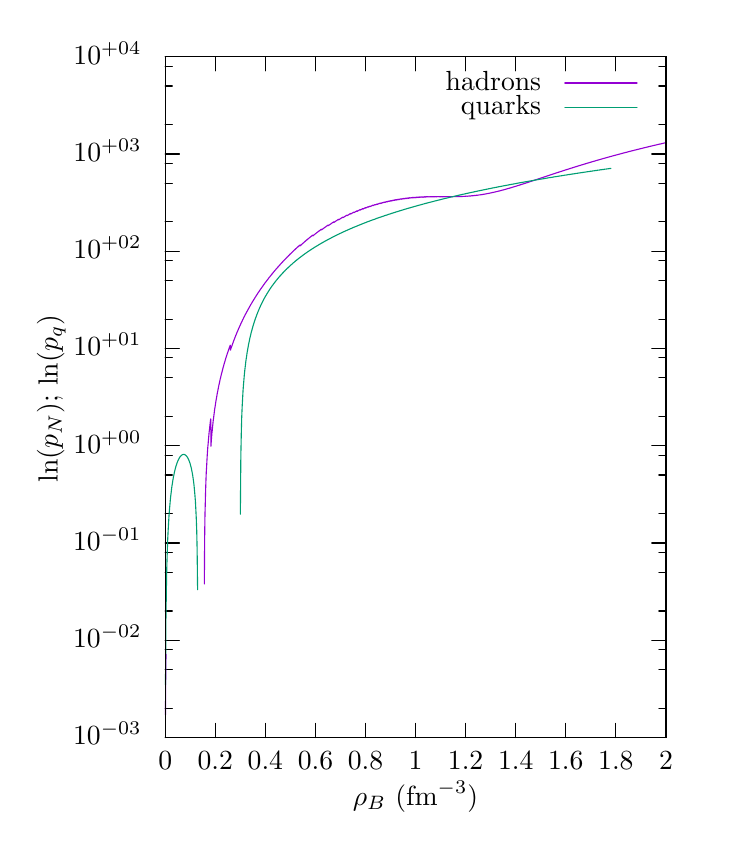
\begin{tikzpicture}[gnuplot]
%% generated with GNUPLOT 5.0p4 (Lua 5.2; terminal rev. 99, script rev. 100)
%% Thu Sep 29 16:33:17 2016
\path (0.000,0.000) rectangle (8.600,10.000);
\gpcolor{color=gp lt color border}
\gpsetlinetype{gp lt border}
\gpsetdashtype{gp dt solid}
\gpsetlinewidth{1.00}
\draw[gp path] (1.688,0.985)--(1.868,0.985);
\draw[gp path] (8.047,0.985)--(7.867,0.985);
\node[gp node right] at (1.504,0.985) {$10^{-03}$};
\draw[gp path] (1.688,1.357)--(1.778,1.357);
\draw[gp path] (8.047,1.357)--(7.957,1.357);
\draw[gp path] (1.688,1.848)--(1.778,1.848);
\draw[gp path] (8.047,1.848)--(7.957,1.848);
\draw[gp path] (1.688,2.100)--(1.778,2.100);
\draw[gp path] (8.047,2.100)--(7.957,2.100);
\draw[gp path] (1.688,2.220)--(1.868,2.220);
\draw[gp path] (8.047,2.220)--(7.867,2.220);
\node[gp node right] at (1.504,2.220) {$10^{-02}$};
\draw[gp path] (1.688,2.592)--(1.778,2.592);
\draw[gp path] (8.047,2.592)--(7.957,2.592);
\draw[gp path] (1.688,3.083)--(1.778,3.083);
\draw[gp path] (8.047,3.083)--(7.957,3.083);
\draw[gp path] (1.688,3.336)--(1.778,3.336);
\draw[gp path] (8.047,3.336)--(7.957,3.336);
\draw[gp path] (1.688,3.455)--(1.868,3.455);
\draw[gp path] (8.047,3.455)--(7.867,3.455);
\node[gp node right] at (1.504,3.455) {$10^{-01}$};
\draw[gp path] (1.688,3.827)--(1.778,3.827);
\draw[gp path] (8.047,3.827)--(7.957,3.827);
\draw[gp path] (1.688,4.319)--(1.778,4.319);
\draw[gp path] (8.047,4.319)--(7.957,4.319);
\draw[gp path] (1.688,4.571)--(1.778,4.571);
\draw[gp path] (8.047,4.571)--(7.957,4.571);
\draw[gp path] (1.688,4.690)--(1.868,4.690);
\draw[gp path] (8.047,4.690)--(7.867,4.690);
\node[gp node right] at (1.504,4.690) {$10^{+00}$};
\draw[gp path] (1.688,5.062)--(1.778,5.062);
\draw[gp path] (8.047,5.062)--(7.957,5.062);
\draw[gp path] (1.688,5.554)--(1.778,5.554);
\draw[gp path] (8.047,5.554)--(7.957,5.554);
\draw[gp path] (1.688,5.806)--(1.778,5.806);
\draw[gp path] (8.047,5.806)--(7.957,5.806);
\draw[gp path] (1.688,5.926)--(1.868,5.926);
\draw[gp path] (8.047,5.926)--(7.867,5.926);
\node[gp node right] at (1.504,5.926) {$10^{+01}$};
\draw[gp path] (1.688,6.297)--(1.778,6.297);
\draw[gp path] (8.047,6.297)--(7.957,6.297);
\draw[gp path] (1.688,6.789)--(1.778,6.789);
\draw[gp path] (8.047,6.789)--(7.957,6.789);
\draw[gp path] (1.688,7.041)--(1.778,7.041);
\draw[gp path] (8.047,7.041)--(7.957,7.041);
\draw[gp path] (1.688,7.161)--(1.868,7.161);
\draw[gp path] (8.047,7.161)--(7.867,7.161);
\node[gp node right] at (1.504,7.161) {$10^{+02}$};
\draw[gp path] (1.688,7.533)--(1.778,7.533);
\draw[gp path] (8.047,7.533)--(7.957,7.533);
\draw[gp path] (1.688,8.024)--(1.778,8.024);
\draw[gp path] (8.047,8.024)--(7.957,8.024);
\draw[gp path] (1.688,8.276)--(1.778,8.276);
\draw[gp path] (8.047,8.276)--(7.957,8.276);
\draw[gp path] (1.688,8.396)--(1.868,8.396);
\draw[gp path] (8.047,8.396)--(7.867,8.396);
\node[gp node right] at (1.504,8.396) {$10^{+03}$};
\draw[gp path] (1.688,8.768)--(1.778,8.768);
\draw[gp path] (8.047,8.768)--(7.957,8.768);
\draw[gp path] (1.688,9.259)--(1.778,9.259);
\draw[gp path] (8.047,9.259)--(7.957,9.259);
\draw[gp path] (1.688,9.511)--(1.778,9.511);
\draw[gp path] (8.047,9.511)--(7.957,9.511);
\draw[gp path] (1.688,9.631)--(1.868,9.631);
\draw[gp path] (8.047,9.631)--(7.867,9.631);
\node[gp node right] at (1.504,9.631) {$10^{+04}$};
\draw[gp path] (1.688,0.985)--(1.688,1.165);
\draw[gp path] (1.688,9.631)--(1.688,9.451);
\node[gp node center] at (1.688,0.677) {$0$};
\draw[gp path] (2.324,0.985)--(2.324,1.165);
\draw[gp path] (2.324,9.631)--(2.324,9.451);
\node[gp node center] at (2.324,0.677) {$0.2$};
\draw[gp path] (2.960,0.985)--(2.960,1.165);
\draw[gp path] (2.960,9.631)--(2.960,9.451);
\node[gp node center] at (2.960,0.677) {$0.4$};
\draw[gp path] (3.596,0.985)--(3.596,1.165);
\draw[gp path] (3.596,9.631)--(3.596,9.451);
\node[gp node center] at (3.596,0.677) {$0.6$};
\draw[gp path] (4.232,0.985)--(4.232,1.165);
\draw[gp path] (4.232,9.631)--(4.232,9.451);
\node[gp node center] at (4.232,0.677) {$0.8$};
\draw[gp path] (4.868,0.985)--(4.868,1.165);
\draw[gp path] (4.868,9.631)--(4.868,9.451);
\node[gp node center] at (4.868,0.677) {$1$};
\draw[gp path] (5.503,0.985)--(5.503,1.165);
\draw[gp path] (5.503,9.631)--(5.503,9.451);
\node[gp node center] at (5.503,0.677) {$1.2$};
\draw[gp path] (6.139,0.985)--(6.139,1.165);
\draw[gp path] (6.139,9.631)--(6.139,9.451);
\node[gp node center] at (6.139,0.677) {$1.4$};
\draw[gp path] (6.775,0.985)--(6.775,1.165);
\draw[gp path] (6.775,9.631)--(6.775,9.451);
\node[gp node center] at (6.775,0.677) {$1.6$};
\draw[gp path] (7.411,0.985)--(7.411,1.165);
\draw[gp path] (7.411,9.631)--(7.411,9.451);
\node[gp node center] at (7.411,0.677) {$1.8$};
\draw[gp path] (8.047,0.985)--(8.047,1.165);
\draw[gp path] (8.047,9.631)--(8.047,9.451);
\node[gp node center] at (8.047,0.677) {$2$};
\draw[gp path] (1.688,9.631)--(1.688,0.985)--(8.047,0.985)--(8.047,9.631)--cycle;
\node[gp node center,rotate=-270] at (0.246,5.308) {$\ln(p_N)$; $\ln(p_q)$};
\node[gp node center] at (4.867,0.215) {$\rho_B$ ($\rm{fm}^{-3}$)};
\node[gp node right] at (6.579,9.297) {hadrons};
\gpcolor{rgb color={0.580,0.000,0.827}}
\draw[gp path] (6.763,9.297)--(7.679,9.297);
\draw[gp path] (1.691,1.272)--(1.693,1.627)--(1.695,1.864)--(1.698,2.043);
\draw[gp path] (2.185,2.934)--(2.187,3.324)--(2.189,3.549)--(2.191,3.709)--(2.193,3.833)%
  --(2.196,3.934)--(2.198,4.021)--(2.200,4.096)--(2.202,4.162)--(2.204,4.222)--(2.206,4.276)%
  --(2.208,4.326)--(2.210,4.372)--(2.213,4.414)--(2.215,4.454)--(2.217,4.492)--(2.219,4.527)%
  --(2.221,4.561)--(2.223,4.592)--(2.225,4.623)--(2.227,4.652)--(2.229,4.679)--(2.232,4.706)%
  --(2.234,4.731)--(2.236,4.756)--(2.238,4.780)--(2.240,4.803)--(2.242,4.825)--(2.244,4.847)%
  --(2.246,4.867)--(2.249,4.888)--(2.251,4.907)--(2.253,4.926)--(2.255,4.945)--(2.257,4.963)%
  --(2.259,4.981)--(2.261,4.998)--(2.263,5.015)--(2.266,5.032)--(2.268,4.683)--(2.270,4.712)%
  --(2.272,4.740)--(2.274,4.766)--(2.276,4.792)--(2.278,4.817)--(2.280,4.841)--(2.282,4.864)%
  --(2.285,4.886)--(2.287,4.907)--(2.289,4.928)--(2.291,4.948)--(2.293,4.968)--(2.295,4.987)%
  --(2.297,5.006)--(2.299,5.024)--(2.302,5.041)--(2.304,5.059)--(2.306,5.076)--(2.308,5.092)%
  --(2.310,5.108)--(2.312,5.124)--(2.314,5.139)--(2.316,5.154)--(2.318,5.169)--(2.321,5.184)%
  --(2.323,5.198)--(2.325,5.212)--(2.327,5.225)--(2.329,5.239)--(2.331,5.252)--(2.333,5.265)%
  --(2.335,5.278)--(2.338,5.290)--(2.340,5.303)--(2.342,5.315)--(2.344,5.327)--(2.346,5.339)%
  --(2.348,5.350)--(2.350,5.362)--(2.352,5.373)--(2.355,5.384)--(2.357,5.395)--(2.359,5.406)%
  --(2.361,5.417)--(2.363,5.427)--(2.365,5.438)--(2.367,5.448)--(2.369,5.458)--(2.371,5.468)%
  --(2.374,5.478)--(2.376,5.488)--(2.378,5.498)--(2.380,5.508)--(2.382,5.517)--(2.384,5.526)%
  --(2.386,5.536)--(2.388,5.545)--(2.391,5.554)--(2.393,5.563)--(2.395,5.572)--(2.397,5.581)%
  --(2.399,5.589)--(2.401,5.598)--(2.403,5.607)--(2.405,5.615)--(2.408,5.623)--(2.410,5.632)%
  --(2.412,5.640)--(2.414,5.648)--(2.416,5.656)--(2.418,5.664)--(2.420,5.672)--(2.422,5.680)%
  --(2.424,5.688)--(2.427,5.696)--(2.429,5.703)--(2.431,5.711)--(2.433,5.718)--(2.435,5.726)%
  --(2.437,5.733)--(2.439,5.741)--(2.441,5.748)--(2.444,5.755)--(2.446,5.762)--(2.448,5.770)%
  --(2.450,5.777)--(2.452,5.784)--(2.454,5.791)--(2.456,5.798)--(2.458,5.804)--(2.460,5.811)%
  --(2.463,5.818)--(2.465,5.825)--(2.467,5.831)--(2.469,5.838)--(2.471,5.845)--(2.473,5.851)%
  --(2.475,5.858)--(2.477,5.864)--(2.480,5.871)--(2.482,5.877)--(2.484,5.883)--(2.486,5.890)%
  --(2.488,5.896)--(2.490,5.902)--(2.492,5.908)--(2.494,5.914)--(2.497,5.921)--(2.499,5.927)%
  --(2.501,5.933)--(2.503,5.939)--(2.505,5.945)--(2.507,5.950)--(2.509,5.956)--(2.511,5.962)%
  --(2.513,5.968)--(2.516,5.904)--(2.518,5.910)--(2.520,5.917)--(2.522,5.923)--(2.524,5.929)%
  --(2.526,5.936)--(2.528,5.942)--(2.530,5.948)--(2.533,5.954)--(2.535,5.960)--(2.537,5.966)%
  --(2.539,5.972)--(2.541,5.978)--(2.543,5.984)--(2.545,5.990)--(2.547,5.995)--(2.550,6.001)%
  --(2.552,6.007)--(2.554,6.013)--(2.556,6.018)--(2.558,6.024)--(2.560,6.030)--(2.562,6.035)%
  --(2.564,6.041)--(2.566,6.046)--(2.569,6.052)--(2.571,6.057)--(2.573,6.063)--(2.575,6.068)%
  --(2.577,6.074)--(2.579,6.079)--(2.581,6.084)--(2.583,6.090)--(2.586,6.095)--(2.588,6.100)%
  --(2.590,6.105)--(2.592,6.111)--(2.594,6.116)--(2.596,6.121)--(2.598,6.126)--(2.600,6.131)%
  --(2.602,6.136)--(2.605,6.141)--(2.607,6.146)--(2.609,6.151)--(2.611,6.156)--(2.613,6.161)%
  --(2.615,6.166)--(2.617,6.171)--(2.619,6.176)--(2.622,6.181)--(2.624,6.185)--(2.626,6.190)%
  --(2.628,6.195)--(2.630,6.200)--(2.632,6.204)--(2.634,6.209)--(2.636,6.214)--(2.639,6.219)%
  --(2.641,6.223)--(2.643,6.228)--(2.645,6.232)--(2.647,6.237)--(2.649,6.242)--(2.651,6.246)%
  --(2.653,6.251)--(2.655,6.255)--(2.658,6.260)--(2.660,6.264)--(2.662,6.269)--(2.664,6.273)%
  --(2.666,6.277)--(2.668,6.282)--(2.670,6.286)--(2.672,6.291)--(2.675,6.295)--(2.677,6.299)%
  --(2.679,6.304)--(2.681,6.308)--(2.683,6.312)--(2.685,6.316)--(2.687,6.321)--(2.689,6.325)%
  --(2.691,6.329)--(2.694,6.333)--(2.696,6.337)--(2.698,6.342)--(2.700,6.346)--(2.702,6.350)%
  --(2.704,6.354)--(2.706,6.358)--(2.708,6.362)--(2.711,6.366)--(2.713,6.370)--(2.715,6.374)%
  --(2.717,6.378)--(2.719,6.382)--(2.721,6.386)--(2.723,6.390)--(2.725,6.394)--(2.728,6.398)%
  --(2.730,6.402)--(2.732,6.406)--(2.734,6.410)--(2.736,6.414)--(2.738,6.418)--(2.740,6.422)%
  --(2.742,6.425)--(2.744,6.429)--(2.747,6.433)--(2.749,6.437)--(2.751,6.441)--(2.753,6.445)%
  --(2.755,6.448)--(2.757,6.452)--(2.759,6.456)--(2.761,6.460)--(2.764,6.463)--(2.766,6.467)%
  --(2.768,6.471)--(2.770,6.474)--(2.772,6.478)--(2.774,6.482)--(2.776,6.485)--(2.778,6.489)%
  --(2.781,6.493)--(2.783,6.496)--(2.785,6.500)--(2.787,6.503)--(2.789,6.507)--(2.791,6.511)%
  --(2.793,6.514)--(2.795,6.518)--(2.797,6.521)--(2.800,6.525)--(2.802,6.528)--(2.804,6.532)%
  --(2.806,6.535)--(2.808,6.539)--(2.810,6.542)--(2.812,6.546)--(2.814,6.549)--(2.817,6.552)%
  --(2.819,6.556)--(2.821,6.559)--(2.823,6.563)--(2.825,6.566)--(2.827,6.569)--(2.829,6.573)%
  --(2.831,6.576)--(2.833,6.580)--(2.836,6.583)--(2.838,6.586)--(2.840,6.590)--(2.842,6.593)%
  --(2.844,6.596)--(2.846,6.599)--(2.848,6.603)--(2.850,6.606)--(2.853,6.609)--(2.855,6.613)%
  --(2.857,6.616)--(2.859,6.619)--(2.861,6.622)--(2.863,6.625)--(2.865,6.629)--(2.867,6.632)%
  --(2.870,6.635)--(2.872,6.638)--(2.874,6.641)--(2.876,6.645)--(2.878,6.648)--(2.880,6.651)%
  --(2.882,6.654)--(2.884,6.657)--(2.886,6.660)--(2.889,6.663)--(2.891,6.667)--(2.893,6.670)%
  --(2.895,6.673)--(2.897,6.676)--(2.899,6.679)--(2.901,6.682)--(2.903,6.685)--(2.906,6.688)%
  --(2.908,6.691)--(2.910,6.694)--(2.912,6.697)--(2.914,6.700)--(2.916,6.703)--(2.918,6.706)%
  --(2.920,6.709)--(2.923,6.712)--(2.925,6.715)--(2.927,6.718)--(2.929,6.721)--(2.931,6.724)%
  --(2.933,6.727)--(2.935,6.730)--(2.937,6.733)--(2.939,6.736)--(2.942,6.739)--(2.944,6.742)%
  --(2.946,6.744)--(2.948,6.747)--(2.950,6.750)--(2.952,6.753)--(2.954,6.756)--(2.956,6.759)%
  --(2.959,6.762)--(2.961,6.765)--(2.963,6.767)--(2.965,6.770)--(2.967,6.773)--(2.969,6.776)%
  --(2.971,6.779)--(2.973,6.781)--(2.975,6.784)--(2.978,6.787)--(2.980,6.790)--(2.982,6.793)%
  --(2.984,6.795)--(2.986,6.798)--(2.988,6.801)--(2.990,6.804)--(2.992,6.806)--(2.995,6.809)%
  --(2.997,6.812)--(2.999,6.815)--(3.001,6.817)--(3.003,6.820)--(3.005,6.823)--(3.007,6.826)%
  --(3.009,6.828)--(3.012,6.831)--(3.014,6.834)--(3.016,6.836)--(3.018,6.839)--(3.020,6.842)%
  --(3.022,6.844)--(3.024,6.847)--(3.026,6.850)--(3.028,6.852)--(3.031,6.855)--(3.033,6.857)%
  --(3.035,6.860)--(3.037,6.863)--(3.039,6.865)--(3.041,6.868)--(3.043,6.871)--(3.045,6.873)%
  --(3.048,6.876)--(3.050,6.878)--(3.052,6.881)--(3.054,6.883)--(3.056,6.886)--(3.058,6.889)%
  --(3.060,6.891)--(3.062,6.894)--(3.064,6.896)--(3.067,6.899)--(3.069,6.901)--(3.071,6.904)%
  --(3.073,6.906)--(3.075,6.909)--(3.077,6.911)--(3.079,6.914)--(3.081,6.916)--(3.084,6.919)%
  --(3.086,6.921)--(3.088,6.924)--(3.090,6.926)--(3.092,6.929)--(3.094,6.931)--(3.096,6.934)%
  --(3.098,6.936)--(3.101,6.939)--(3.103,6.941)--(3.105,6.944)--(3.107,6.946)--(3.109,6.948)%
  --(3.111,6.951)--(3.113,6.953)--(3.115,6.956)--(3.117,6.958)--(3.120,6.960)--(3.122,6.963)%
  --(3.124,6.965)--(3.126,6.968)--(3.128,6.970)--(3.130,6.972)--(3.132,6.975)--(3.134,6.977)%
  --(3.137,6.980)--(3.139,6.982)--(3.141,6.984)--(3.143,6.987)--(3.145,6.989)--(3.147,6.991)%
  --(3.149,6.994)--(3.151,6.996)--(3.154,6.998)--(3.156,7.001)--(3.158,7.003)--(3.160,7.005)%
  --(3.162,7.008)--(3.164,7.010)--(3.166,7.012)--(3.168,7.014)--(3.170,7.017)--(3.173,7.019)%
  --(3.175,7.021)--(3.177,7.024)--(3.179,7.026)--(3.181,7.028)--(3.183,7.030)--(3.185,7.033)%
  --(3.187,7.035)--(3.190,7.037)--(3.192,7.039)--(3.194,7.042)--(3.196,7.044)--(3.198,7.046)%
  --(3.200,7.048)--(3.202,7.051)--(3.204,7.053)--(3.206,7.055)--(3.209,7.057)--(3.211,7.059)%
  --(3.213,7.062)--(3.215,7.064)--(3.217,7.066)--(3.219,7.068)--(3.221,7.070)--(3.223,7.073)%
  --(3.226,7.075)--(3.228,7.077)--(3.230,7.079)--(3.232,7.081)--(3.234,7.083)--(3.236,7.086)%
  --(3.238,7.088)--(3.240,7.090)--(3.243,7.092)--(3.245,7.094)--(3.247,7.096)--(3.249,7.098)%
  --(3.251,7.101)--(3.253,7.103)--(3.255,7.105)--(3.257,7.107)--(3.259,7.109)--(3.262,7.111)%
  --(3.264,7.113)--(3.266,7.115)--(3.268,7.118)--(3.270,7.120)--(3.272,7.122)--(3.274,7.124)%
  --(3.276,7.126)--(3.279,7.128)--(3.281,7.130)--(3.283,7.132)--(3.285,7.134)--(3.287,7.136)%
  --(3.289,7.138)--(3.291,7.140)--(3.293,7.142)--(3.295,7.144)--(3.298,7.147)--(3.300,7.149)%
  --(3.302,7.151)--(3.304,7.153)--(3.306,7.155)--(3.308,7.157)--(3.310,7.159)--(3.312,7.161)%
  --(3.315,7.163)--(3.317,7.165)--(3.319,7.167)--(3.321,7.169)--(3.323,7.171)--(3.325,7.173)%
  --(3.327,7.175)--(3.329,7.177)--(3.332,7.179)--(3.334,7.181)--(3.336,7.183)--(3.338,7.185)%
  --(3.340,7.187)--(3.342,7.189)--(3.344,7.191)--(3.346,7.193)--(3.348,7.195)--(3.351,7.197)%
  --(3.353,7.199)--(3.355,7.200)--(3.357,7.202)--(3.359,7.204)--(3.361,7.206)--(3.363,7.208)%
  --(3.365,7.210)--(3.368,7.212)--(3.370,7.214)--(3.372,7.216)--(3.374,7.218)--(3.376,7.220)%
  --(3.378,7.222)--(3.380,7.224)--(3.382,7.226)--(3.385,7.227)--(3.387,7.229)--(3.389,7.231)%
  --(3.391,7.233)--(3.393,7.235)--(3.395,7.237)--(3.397,7.239)--(3.399,7.228)--(3.401,7.230)%
  --(3.404,7.232)--(3.406,7.234)--(3.408,7.236)--(3.410,7.238)--(3.412,7.240)--(3.414,7.242)%
  --(3.416,7.244)--(3.418,7.245)--(3.421,7.247)--(3.423,7.249)--(3.425,7.251)--(3.427,7.253)%
  --(3.429,7.255)--(3.431,7.257)--(3.433,7.259)--(3.435,7.260)--(3.437,7.262)--(3.440,7.264)%
  --(3.442,7.266)--(3.444,7.268)--(3.446,7.270)--(3.448,7.271)--(3.450,7.273)--(3.452,7.275)%
  --(3.454,7.277)--(3.457,7.279)--(3.459,7.281)--(3.461,7.282)--(3.463,7.284)--(3.465,7.286)%
  --(3.467,7.288)--(3.469,7.290)--(3.471,7.292)--(3.474,7.293)--(3.476,7.295)--(3.478,7.297)%
  --(3.480,7.299)--(3.482,7.301)--(3.484,7.302)--(3.486,7.304)--(3.488,7.306)--(3.490,7.308)%
  --(3.493,7.309)--(3.495,7.311)--(3.497,7.313)--(3.499,7.315)--(3.501,7.317)--(3.503,7.318)%
  --(3.505,7.320)--(3.507,7.322)--(3.510,7.324)--(3.512,7.325)--(3.514,7.327)--(3.516,7.329)%
  --(3.518,7.331)--(3.520,7.332)--(3.522,7.334)--(3.524,7.336)--(3.527,7.338)--(3.529,7.339)%
  --(3.531,7.341)--(3.533,7.343)--(3.535,7.345)--(3.537,7.346)--(3.539,7.348)--(3.541,7.350)%
  --(3.543,7.351)--(3.546,7.353)--(3.548,7.355)--(3.550,7.357)--(3.552,7.358)--(3.554,7.360)%
  --(3.556,7.362)--(3.558,7.363)--(3.560,7.365)--(3.563,7.356)--(3.565,7.358)--(3.567,7.359)%
  --(3.569,7.361)--(3.571,7.363)--(3.573,7.365)--(3.575,7.366)--(3.577,7.368)--(3.579,7.370)%
  --(3.582,7.371)--(3.584,7.373)--(3.586,7.375)--(3.588,7.376)--(3.590,7.378)--(3.592,7.380)%
  --(3.594,7.381)--(3.596,7.383)--(3.599,7.385)--(3.601,7.386)--(3.603,7.388)--(3.605,7.390)%
  --(3.607,7.391)--(3.609,7.393)--(3.611,7.395)--(3.613,7.396)--(3.616,7.398)--(3.618,7.400)%
  --(3.620,7.401)--(3.622,7.403)--(3.624,7.405)--(3.626,7.406)--(3.628,7.408)--(3.630,7.409)%
  --(3.632,7.411)--(3.635,7.413)--(3.637,7.414)--(3.639,7.416)--(3.641,7.418)--(3.643,7.419)%
  --(3.645,7.421)--(3.647,7.422)--(3.649,7.424)--(3.652,7.426)--(3.654,7.427)--(3.656,7.429)%
  --(3.658,7.430)--(3.660,7.432)--(3.662,7.434)--(3.664,7.435)--(3.666,7.437)--(3.668,7.438)%
  --(3.671,7.440)--(3.673,7.432)--(3.675,7.433)--(3.677,7.435)--(3.679,7.436)--(3.681,7.438)%
  --(3.683,7.440)--(3.685,7.441)--(3.688,7.443)--(3.690,7.444)--(3.692,7.446)--(3.694,7.448)%
  --(3.696,7.449)--(3.698,7.451)--(3.700,7.452)--(3.702,7.454)--(3.705,7.455)--(3.707,7.457)%
  --(3.709,7.459)--(3.711,7.460)--(3.713,7.462)--(3.715,7.463)--(3.717,7.465)--(3.719,7.466)%
  --(3.721,7.468)--(3.724,7.469)--(3.726,7.471)--(3.728,7.472)--(3.730,7.474)--(3.732,7.476)%
  --(3.734,7.477)--(3.736,7.479)--(3.738,7.480)--(3.741,7.482)--(3.743,7.483)--(3.745,7.485)%
  --(3.747,7.486)--(3.749,7.488)--(3.751,7.489)--(3.753,7.491)--(3.755,7.492)--(3.758,7.485)%
  --(3.760,7.486)--(3.762,7.488)--(3.764,7.489)--(3.766,7.491)--(3.768,7.492)--(3.770,7.494)%
  --(3.772,7.495)--(3.774,7.497)--(3.777,7.498)--(3.779,7.500)--(3.781,7.501)--(3.783,7.503)%
  --(3.785,7.504)--(3.787,7.506)--(3.789,7.507)--(3.791,7.509)--(3.794,7.510)--(3.796,7.512)%
  --(3.798,7.513)--(3.800,7.515)--(3.802,7.516)--(3.804,7.518)--(3.806,7.519)--(3.808,7.521)%
  --(3.810,7.522)--(3.813,7.523)--(3.815,7.525)--(3.817,7.526)--(3.819,7.528)--(3.821,7.529)%
  --(3.823,7.531)--(3.825,7.532)--(3.827,7.534)--(3.830,7.526)--(3.832,7.528)--(3.834,7.529)%
  --(3.836,7.531)--(3.838,7.532)--(3.840,7.534)--(3.842,7.535)--(3.844,7.536)--(3.847,7.538)%
  --(3.849,7.539)--(3.851,7.541)--(3.853,7.542)--(3.855,7.544)--(3.857,7.545)--(3.859,7.547)%
  --(3.861,7.548)--(3.863,7.549)--(3.866,7.551)--(3.868,7.552)--(3.870,7.554)--(3.872,7.555)%
  --(3.874,7.557)--(3.876,7.558)--(3.878,7.559)--(3.880,7.561)--(3.883,7.562)--(3.885,7.564)%
  --(3.887,7.565)--(3.889,7.567)--(3.891,7.559)--(3.893,7.561)--(3.895,7.562)--(3.897,7.564)%
  --(3.900,7.565)--(3.902,7.566)--(3.904,7.568)--(3.906,7.569)--(3.908,7.571)--(3.910,7.572)%
  --(3.912,7.574)--(3.914,7.575)--(3.916,7.576)--(3.919,7.578)--(3.921,7.579)--(3.923,7.581)%
  --(3.925,7.582)--(3.927,7.583)--(3.929,7.585)--(3.931,7.586)--(3.933,7.587)--(3.936,7.589)%
  --(3.938,7.590)--(3.940,7.592)--(3.942,7.593)--(3.944,7.594)--(3.946,7.587)--(3.948,7.589)%
  --(3.950,7.590)--(3.952,7.592)--(3.955,7.593)--(3.957,7.594)--(3.959,7.596)--(3.961,7.597)%
  --(3.963,7.598)--(3.965,7.600)--(3.967,7.601)--(3.969,7.602)--(3.972,7.604)--(3.974,7.605)%
  --(3.976,7.607)--(3.978,7.608)--(3.980,7.609)--(3.982,7.611)--(3.984,7.612)--(3.986,7.613)%
  --(3.989,7.615)--(3.991,7.616)--(3.993,7.617)--(3.995,7.619)--(3.997,7.612)--(3.999,7.613)%
  --(4.001,7.615)--(4.003,7.616)--(4.005,7.617)--(4.008,7.619)--(4.010,7.620)--(4.012,7.621)%
  --(4.014,7.623)--(4.016,7.624)--(4.018,7.625)--(4.020,7.627)--(4.022,7.628)--(4.025,7.629)%
  --(4.027,7.631)--(4.029,7.632)--(4.031,7.633)--(4.033,7.635)--(4.035,7.636)--(4.037,7.637)%
  --(4.039,7.639)--(4.041,7.640)--(4.044,7.633)--(4.046,7.635)--(4.048,7.636)--(4.050,7.637)%
  --(4.052,7.639)--(4.054,7.640)--(4.056,7.641)--(4.058,7.642)--(4.061,7.644)--(4.063,7.645)%
  --(4.065,7.646)--(4.067,7.648)--(4.069,7.649)--(4.071,7.650)--(4.073,7.652)--(4.075,7.653)%
  --(4.078,7.654)--(4.080,7.656)--(4.082,7.657)--(4.084,7.658)--(4.086,7.652)--(4.088,7.653)%
  --(4.090,7.654)--(4.092,7.655)--(4.094,7.657)--(4.097,7.658)--(4.099,7.659)--(4.101,7.661)%
  --(4.103,7.662)--(4.105,7.663)--(4.107,7.664)--(4.109,7.666)--(4.111,7.667)--(4.114,7.668)%
  --(4.116,7.670)--(4.118,7.671)--(4.120,7.672)--(4.122,7.673)--(4.124,7.675)--(4.126,7.668)%
  --(4.128,7.669)--(4.131,7.671)--(4.133,7.672)--(4.135,7.673)--(4.137,7.675)--(4.139,7.676)%
  --(4.141,7.677)--(4.143,7.678)--(4.145,7.680)--(4.147,7.681)--(4.150,7.682)--(4.152,7.683)%
  --(4.154,7.685)--(4.156,7.686)--(4.158,7.687)--(4.160,7.688)--(4.162,7.690)--(4.164,7.683)%
  --(4.167,7.685)--(4.169,7.686)--(4.171,7.687)--(4.173,7.688)--(4.175,7.690)--(4.177,7.691)%
  --(4.179,7.692)--(4.181,7.693)--(4.183,7.695)--(4.186,7.696)--(4.188,7.697)--(4.190,7.698)%
  --(4.192,7.700)--(4.194,7.701)--(4.196,7.702)--(4.198,7.696)--(4.200,7.697)--(4.203,7.698)%
  --(4.205,7.699)--(4.207,7.701)--(4.209,7.702)--(4.211,7.703)--(4.213,7.704)--(4.215,7.706)%
  --(4.217,7.707)--(4.220,7.708)--(4.222,7.709)--(4.224,7.710)--(4.226,7.712)--(4.228,7.713)%
  --(4.230,7.714)--(4.232,7.715)--(4.234,7.709)--(4.236,7.710)--(4.239,7.712)--(4.241,7.713)%
  --(4.243,7.714)--(4.245,7.715)--(4.247,7.716)--(4.249,7.718)--(4.251,7.719)--(4.253,7.720)%
  --(4.256,7.721)--(4.258,7.722)--(4.260,7.724)--(4.262,7.725)--(4.264,7.726)--(4.266,7.720)%
  --(4.268,7.721)--(4.270,7.722)--(4.273,7.723)--(4.275,7.725)--(4.277,7.726)--(4.279,7.727)%
  --(4.281,7.728)--(4.283,7.730)--(4.285,7.731)--(4.287,7.732)--(4.289,7.733)--(4.292,7.734)%
  --(4.294,7.735)--(4.296,7.729)--(4.298,7.731)--(4.300,7.732)--(4.302,7.733)--(4.304,7.734)%
  --(4.306,7.735)--(4.309,7.736)--(4.311,7.738)--(4.313,7.739)--(4.315,7.740)--(4.317,7.741)%
  --(4.319,7.742)--(4.321,7.744)--(4.323,7.745)--(4.325,7.746)--(4.328,7.740)--(4.330,7.741)%
  --(4.332,7.742)--(4.334,7.743)--(4.336,7.745)--(4.338,7.746)--(4.340,7.747)--(4.342,7.748)%
  --(4.345,7.749)--(4.347,7.750)--(4.349,7.752)--(4.351,7.753)--(4.353,7.754)--(4.355,7.748)%
  --(4.357,7.749)--(4.359,7.750)--(4.362,7.751)--(4.364,7.753)--(4.366,7.754)--(4.368,7.755)%
  --(4.370,7.756)--(4.372,7.757)--(4.374,7.758)--(4.376,7.759)--(4.378,7.761)--(4.381,7.762)%
  --(4.383,7.756)--(4.385,7.757)--(4.387,7.758)--(4.389,7.759)--(4.391,7.760)--(4.393,7.762)%
  --(4.395,7.763)--(4.398,7.764)--(4.400,7.765)--(4.402,7.766)--(4.404,7.767)--(4.406,7.768)%
  --(4.408,7.770)--(4.410,7.764)--(4.412,7.765)--(4.414,7.766)--(4.417,7.767)--(4.419,7.768)%
  --(4.421,7.769)--(4.423,7.770)--(4.425,7.772)--(4.427,7.773)--(4.429,7.774)--(4.431,7.775)%
  --(4.434,7.776)--(4.436,7.770)--(4.438,7.771)--(4.440,7.772)--(4.442,7.774)--(4.444,7.775)%
  --(4.446,7.776)--(4.448,7.777)--(4.451,7.778)--(4.453,7.779)--(4.455,7.780)--(4.457,7.781)%
  --(4.459,7.783)--(4.461,7.777)--(4.463,7.778)--(4.465,7.779)--(4.467,7.780)--(4.470,7.781)%
  --(4.472,7.782)--(4.474,7.783)--(4.476,7.785)--(4.478,7.786)--(4.480,7.787)--(4.482,7.788)%
  --(4.484,7.782)--(4.487,7.783)--(4.489,7.784)--(4.491,7.785)--(4.493,7.786)--(4.495,7.788)%
  --(4.497,7.789)--(4.499,7.790)--(4.501,7.791)--(4.504,7.792)--(4.506,7.793)--(4.508,7.794)%
  --(4.510,7.788)--(4.512,7.789)--(4.514,7.790)--(4.516,7.792)--(4.518,7.793)--(4.520,7.794)%
  --(4.523,7.795)--(4.525,7.796)--(4.527,7.797)--(4.529,7.798)--(4.531,7.799)--(4.533,7.793)%
  --(4.535,7.795)--(4.537,7.796)--(4.540,7.797)--(4.542,7.798)--(4.544,7.799)--(4.546,7.800)%
  --(4.548,7.801)--(4.550,7.802)--(4.552,7.803)--(4.554,7.797)--(4.556,7.798)--(4.559,7.800)%
  --(4.561,7.801)--(4.563,7.802)--(4.565,7.803)--(4.567,7.804)--(4.569,7.805)--(4.571,7.806)%
  --(4.573,7.807)--(4.576,7.808)--(4.578,7.802)--(4.580,7.804)--(4.582,7.805)--(4.584,7.806)%
  --(4.586,7.807)--(4.588,7.808)--(4.590,7.809)--(4.593,7.810)--(4.595,7.811)--(4.597,7.812)%
  --(4.599,7.806)--(4.601,7.807)--(4.603,7.808)--(4.605,7.810)--(4.607,7.811)--(4.609,7.812)%
  --(4.612,7.813)--(4.614,7.814)--(4.616,7.815)--(4.618,7.816)--(4.620,7.810)--(4.622,7.811)%
  --(4.624,7.812)--(4.626,7.813)--(4.629,7.814)--(4.631,7.816)--(4.633,7.817)--(4.635,7.818)%
  --(4.637,7.819)--(4.639,7.820)--(4.641,7.814)--(4.643,7.815)--(4.646,7.816)--(4.648,7.817)%
  --(4.650,7.818)--(4.652,7.819)--(4.654,7.820)--(4.656,7.821)--(4.658,7.822)--(4.660,7.817)%
  --(4.662,7.818)--(4.665,7.819)--(4.667,7.820)--(4.669,7.821)--(4.671,7.822)--(4.673,7.823)%
  --(4.675,7.824)--(4.677,7.825)--(4.679,7.826)--(4.682,7.820)--(4.684,7.821)--(4.686,7.822)%
  --(4.688,7.823)--(4.690,7.825)--(4.692,7.826)--(4.694,7.827)--(4.696,7.828)--(4.698,7.829)%
  --(4.701,7.823)--(4.703,7.824)--(4.705,7.825)--(4.707,7.826)--(4.709,7.827)--(4.711,7.828)%
  --(4.713,7.829)--(4.715,7.830)--(4.718,7.831)--(4.720,7.825)--(4.722,7.826)--(4.724,7.828)%
  --(4.726,7.829)--(4.728,7.830)--(4.730,7.831)--(4.732,7.832)--(4.735,7.833)--(4.737,7.834)%
  --(4.739,7.828)--(4.741,7.829)--(4.743,7.830)--(4.745,7.831)--(4.747,7.832)--(4.749,7.833)%
  --(4.751,7.834)--(4.754,7.835)--(4.756,7.836)--(4.758,7.830)--(4.760,7.831)--(4.762,7.833)%
  --(4.764,7.834)--(4.766,7.835)--(4.768,7.836)--(4.771,7.837)--(4.773,7.838)--(4.775,7.839)%
  --(4.777,7.833)--(4.779,7.834)--(4.781,7.835)--(4.783,7.836)--(4.785,7.837)--(4.787,7.838)%
  --(4.790,7.839)--(4.792,7.840)--(4.794,7.834)--(4.796,7.835)--(4.798,7.836)--(4.800,7.837)%
  --(4.802,7.838)--(4.804,7.839)--(4.807,7.840)--(4.809,7.841)--(4.811,7.842)--(4.813,7.837)%
  --(4.815,7.838)--(4.817,7.839)--(4.819,7.840)--(4.821,7.841)--(4.824,7.842)--(4.826,7.843)%
  --(4.828,7.844)--(4.830,7.838)--(4.832,7.839)--(4.834,7.840)--(4.836,7.841)--(4.838,7.842)%
  --(4.840,7.843)--(4.843,7.844)--(4.845,7.845)--(4.847,7.839)--(4.849,7.840)--(4.851,7.841)%
  --(4.853,7.842)--(4.855,7.843)--(4.857,7.844)--(4.860,7.845)--(4.862,7.846)--(4.864,7.840)%
  --(4.866,7.841)--(4.868,7.842)--(4.870,7.843)--(4.872,7.845)--(4.874,7.846)--(4.877,7.847)%
  --(4.879,7.848)--(4.881,7.842)--(4.883,7.843)--(4.885,7.844)--(4.887,7.845)--(4.889,7.846)%
  --(4.891,7.847)--(4.893,7.848)--(4.896,7.849)--(4.898,7.843)--(4.900,7.844)--(4.902,7.845)%
  --(4.904,7.846)--(4.906,7.847)--(4.908,7.848)--(4.910,7.849)--(4.913,7.850)--(4.915,7.844)%
  --(4.917,7.845)--(4.919,7.846)--(4.921,7.847)--(4.923,7.848)--(4.925,7.849)--(4.927,7.850)%
  --(4.929,7.851)--(4.932,7.845)--(4.934,7.846)--(4.936,7.847)--(4.938,7.848)--(4.940,7.849)%
  --(4.942,7.850)--(4.944,7.851)--(4.946,7.852)--(4.949,7.846)--(4.951,7.847)--(4.953,7.848)%
  --(4.955,7.849)--(4.957,7.850)--(4.959,7.851)--(4.961,7.852)--(4.963,7.846)--(4.966,7.847)%
  --(4.968,7.848)--(4.970,7.849)--(4.972,7.850)--(4.974,7.851)--(4.976,7.852)--(4.978,7.853)%
  --(4.980,7.847)--(4.982,7.848)--(4.985,7.849)--(4.987,7.850)--(4.989,7.851)--(4.991,7.852)%
  --(4.993,7.853)--(4.995,7.848)--(4.997,7.849)--(4.999,7.850)--(5.002,7.851)--(5.004,7.852)%
  --(5.006,7.853)--(5.008,7.854)--(5.010,7.855)--(5.012,7.850)--(5.014,7.851)--(5.016,7.852)%
  --(5.019,7.853)--(5.021,7.851)--(5.023,7.852)--(5.025,7.853)--(5.027,7.850)--(5.029,7.851)%
  --(5.031,7.852)--(5.033,7.853)--(5.035,7.851)--(5.038,7.852)--(5.040,7.853)--(5.042,7.854)%
  --(5.044,7.851)--(5.046,7.852)--(5.048,7.853)--(5.050,7.851)--(5.052,7.852)--(5.055,7.853)%
  --(5.057,7.854)--(5.059,7.851)--(5.061,7.852)--(5.063,7.853)--(5.065,7.854)--(5.067,7.852)%
  --(5.069,7.853)--(5.071,7.854)--(5.074,7.851)--(5.076,7.852)--(5.078,7.853)--(5.080,7.854)%
  --(5.082,7.852)--(5.084,7.853)--(5.086,7.854)--(5.088,7.855)--(5.091,7.852)--(5.093,7.853)%
  --(5.095,7.854)--(5.097,7.852)--(5.099,7.853)--(5.101,7.854)--(5.103,7.855)--(5.105,7.852)%
  --(5.108,7.853)--(5.110,7.854)--(5.112,7.852)--(5.114,7.853)--(5.116,7.854)--(5.118,7.855)%
  --(5.120,7.852)--(5.122,7.853)--(5.124,7.854)--(5.127,7.852)--(5.129,7.853)--(5.131,7.854)%
  --(5.133,7.855)--(5.135,7.852)--(5.137,7.853)--(5.139,7.854)--(5.141,7.855)--(5.144,7.853)%
  --(5.146,7.854)--(5.148,7.855)--(5.150,7.852)--(5.152,7.853)--(5.154,7.854)--(5.156,7.855)%
  --(5.158,7.853)--(5.160,7.854)--(5.163,7.855)--(5.165,7.852)--(5.167,7.853)--(5.169,7.854)%
  --(5.171,7.855)--(5.173,7.853)--(5.175,7.854)--(5.177,7.854)--(5.180,7.852)--(5.182,7.853)%
  --(5.184,7.854)--(5.186,7.855)--(5.188,7.852)--(5.190,7.853)--(5.192,7.854)--(5.194,7.852)%
  --(5.197,7.853)--(5.199,7.854)--(5.201,7.855)--(5.203,7.852)--(5.205,7.853)--(5.207,7.854)%
  --(5.209,7.852)--(5.211,7.853)--(5.213,7.854)--(5.216,7.855)--(5.218,7.852)--(5.220,7.853)%
  --(5.222,7.854)--(5.224,7.852)--(5.226,7.853)--(5.228,7.854)--(5.230,7.855)--(5.233,7.852)%
  --(5.235,7.853)--(5.237,7.854)--(5.239,7.855)--(5.241,7.853)--(5.243,7.854)--(5.245,7.855)%
  --(5.247,7.852)--(5.250,7.853)--(5.252,7.854)--(5.254,7.855)--(5.256,7.853)--(5.258,7.854)%
  --(5.260,7.855)--(5.262,7.852)--(5.264,7.853)--(5.266,7.854)--(5.269,7.855)--(5.271,7.853)%
  --(5.273,7.854)--(5.275,7.855)--(5.277,7.852)--(5.279,7.853)--(5.281,7.854)--(5.283,7.855)%
  --(5.286,7.853)--(5.288,7.854)--(5.290,7.855)--(5.292,7.852)--(5.294,7.853)--(5.296,7.854)%
  --(5.298,7.855)--(5.300,7.853)--(5.302,7.854)--(5.305,7.855)--(5.307,7.852)--(5.309,7.853)%
  --(5.311,7.854)--(5.313,7.855)--(5.315,7.853)--(5.317,7.854)--(5.319,7.855)--(5.322,7.852)%
  --(5.324,7.853)--(5.326,7.854)--(5.328,7.855)--(5.330,7.853)--(5.332,7.854)--(5.334,7.855)%
  --(5.336,7.852)--(5.339,7.853)--(5.341,7.854)--(5.343,7.855)--(5.345,7.853)--(5.347,7.854)%
  --(5.349,7.855)--(5.351,7.855)--(5.353,7.853)--(5.355,7.854)--(5.358,7.855)--(5.360,7.853)%
  --(5.362,7.854)--(5.364,7.855)--(5.366,7.856)--(5.368,7.853)--(5.370,7.854)--(5.372,7.855)%
  --(5.375,7.853)--(5.377,7.854)--(5.379,7.855)--(5.381,7.856)--(5.383,7.853)--(5.385,7.854)%
  --(5.387,7.855)--(5.389,7.853)--(5.392,7.854)--(5.394,7.855)--(5.396,7.856)--(5.398,7.853)%
  --(5.400,7.854)--(5.402,7.855)--(5.404,7.856)--(5.406,7.854)--(5.408,7.855)--(5.411,7.856)%
  --(5.413,7.854)--(5.415,7.854)--(5.417,7.855)--(5.419,7.856)--(5.421,7.854)--(5.423,7.855)%
  --(5.425,7.856)--(5.428,7.857)--(5.430,7.855)--(5.432,7.856)--(5.434,7.857)--(5.436,7.854)%
  --(5.438,7.855)--(5.440,7.856)--(5.442,7.857)--(5.444,7.855)--(5.447,7.856)--(5.449,7.857)%
  --(5.451,7.858)--(5.453,7.855)--(5.455,7.856)--(5.457,7.857)--(5.459,7.855)--(5.461,7.856)%
  --(5.464,7.857)--(5.466,7.858)--(5.468,7.856)--(5.470,7.857)--(5.472,7.858)--(5.474,7.859)%
  --(5.476,7.856)--(5.478,7.857)--(5.481,7.858)--(5.483,7.859)--(5.485,7.857)--(5.487,7.858)%
  --(5.489,7.859)--(5.491,7.857)--(5.493,7.858)--(5.495,7.859)--(5.497,7.859)--(5.500,7.857)%
  --(5.502,7.858)--(5.504,7.859)--(5.506,7.860)--(5.508,7.858)--(5.510,7.859)--(5.512,7.860)%
  --(5.514,7.861)--(5.517,7.859)--(5.519,7.860)--(5.521,7.861)--(5.523,7.858)--(5.525,7.859)%
  --(5.527,7.860)--(5.529,7.861)--(5.531,7.859)--(5.533,7.860)--(5.536,7.861)--(5.538,7.862)%
  --(5.540,7.860)--(5.542,7.861)--(5.544,7.862)--(5.546,7.863)--(5.548,7.861)--(5.550,7.861)%
  --(5.553,7.862)--(5.555,7.863)--(5.557,7.861)--(5.559,7.862)--(5.561,7.863)--(5.563,7.864)%
  --(5.565,7.862)--(5.567,7.863)--(5.570,7.864)--(5.572,7.865)--(5.574,7.863)--(5.576,7.864)%
  --(5.578,7.865)--(5.580,7.866)--(5.582,7.864)--(5.584,7.865)--(5.586,7.865)--(5.589,7.866)%
  --(5.591,7.864)--(5.593,7.865)--(5.595,7.866)--(5.597,7.867)--(5.599,7.865)--(5.601,7.866)%
  --(5.603,7.867)--(5.606,7.868)--(5.608,7.866)--(5.610,7.867)--(5.612,7.868)--(5.614,7.869)%
  --(5.616,7.867)--(5.618,7.868)--(5.620,7.869)--(5.623,7.870)--(5.625,7.868)--(5.627,7.869)%
  --(5.629,7.870)--(5.631,7.871)--(5.633,7.869)--(5.635,7.870)--(5.637,7.871)--(5.639,7.871)%
  --(5.642,7.870)--(5.644,7.871)--(5.646,7.871)--(5.648,7.872)--(5.650,7.873)--(5.652,7.871)%
  --(5.654,7.872)--(5.656,7.873)--(5.659,7.874)--(5.661,7.872)--(5.663,7.873)--(5.665,7.874)%
  --(5.667,7.875)--(5.669,7.873)--(5.671,7.874)--(5.673,7.875)--(5.675,7.876)--(5.678,7.877)%
  --(5.680,7.875)--(5.682,7.876)--(5.684,7.877)--(5.686,7.878)--(5.688,7.876)--(5.690,7.877)%
  --(5.692,7.878)--(5.695,7.879)--(5.697,7.877)--(5.699,7.878)--(5.701,7.879)--(5.703,7.880)%
  --(5.705,7.881)--(5.707,7.879)--(5.709,7.880)--(5.712,7.881)--(5.714,7.882)--(5.716,7.880)%
  --(5.718,7.881)--(5.720,7.882)--(5.722,7.883)--(5.724,7.884)--(5.726,7.882)--(5.728,7.883)%
  --(5.731,7.884)--(5.733,7.885)--(5.735,7.884)--(5.737,7.884)--(5.739,7.885)--(5.741,7.886)%
  --(5.743,7.887)--(5.745,7.886)--(5.748,7.887)--(5.750,7.887)--(5.752,7.888)--(5.754,7.887)%
  --(5.756,7.888)--(5.758,7.889)--(5.760,7.890)--(5.762,7.890)--(5.764,7.889)--(5.767,7.890)%
  --(5.769,7.891)--(5.771,7.892)--(5.773,7.892)--(5.775,7.891)--(5.777,7.892)--(5.779,7.893)%
  --(5.781,7.894)--(5.784,7.892)--(5.786,7.893)--(5.788,7.894)--(5.790,7.895)--(5.792,7.896)%
  --(5.794,7.894)--(5.796,7.895)--(5.798,7.896)--(5.801,7.897)--(5.803,7.898)--(5.805,7.897)%
  --(5.807,7.898)--(5.809,7.898)--(5.811,7.899)--(5.813,7.900)--(5.815,7.899)--(5.817,7.900)%
  --(5.820,7.901)--(5.822,7.902)--(5.824,7.902)--(5.826,7.902)--(5.828,7.903)--(5.830,7.902)%
  --(5.832,7.903)--(5.834,7.904)--(5.837,7.904)--(5.839,7.905)--(5.841,7.906)--(5.843,7.906)%
  --(5.845,7.906)--(5.847,7.906)--(5.849,7.907)--(5.851,7.908)--(5.854,7.908)--(5.856,7.909)%
  --(5.858,7.909)--(5.860,7.909)--(5.862,7.910)--(5.864,7.910)--(5.866,7.911)--(5.868,7.911)%
  --(5.870,7.912)--(5.873,7.913)--(5.875,7.913)--(5.877,7.913)--(5.879,7.914)--(5.881,7.914)%
  --(5.883,7.915)--(5.885,7.915)--(5.887,7.916)--(5.890,7.917)--(5.892,7.917)--(5.894,7.917)%
  --(5.896,7.918)--(5.898,7.918)--(5.900,7.919)--(5.902,7.919)--(5.904,7.920)--(5.906,7.921)%
  --(5.909,7.921)--(5.911,7.921)--(5.913,7.922)--(5.915,7.922)--(5.917,7.923)--(5.919,7.924)%
  --(5.921,7.924)--(5.923,7.925)--(5.926,7.925)--(5.928,7.926)--(5.930,7.926)--(5.932,7.926)%
  --(5.934,7.927)--(5.936,7.928)--(5.938,7.928)--(5.940,7.929)--(5.943,7.930)--(5.945,7.930)%
  --(5.947,7.931)--(5.949,7.932)--(5.951,7.931)--(5.953,7.932)--(5.955,7.933)--(5.957,7.933)%
  --(5.959,7.934)--(5.962,7.934)--(5.964,7.935)--(5.966,7.936)--(5.968,7.936)--(5.970,7.937)%
  --(5.972,7.937)--(5.974,7.937)--(5.976,7.938)--(5.979,7.939)--(5.981,7.939)--(5.983,7.940)%
  --(5.985,7.941)--(5.987,7.941)--(5.989,7.942)--(5.991,7.943)--(5.993,7.943)--(5.996,7.944)%
  --(5.998,7.944)--(6.000,7.944)--(6.002,7.945)--(6.004,7.946)--(6.006,7.946)--(6.008,7.947)%
  --(6.010,7.948)--(6.012,7.948)--(6.015,7.949)--(6.017,7.950)--(6.019,7.950)--(6.021,7.951)%
  --(6.023,7.951)--(6.025,7.952)--(6.027,7.952)--(6.029,7.953)--(6.032,7.954)--(6.034,7.954)%
  --(6.036,7.955)--(6.038,7.956)--(6.040,7.956)--(6.042,7.957)--(6.044,7.958)--(6.046,7.958)%
  --(6.048,7.959)--(6.051,7.959)--(6.053,7.960)--(6.055,7.960)--(6.057,7.961)--(6.059,7.961)%
  --(6.061,7.962)--(6.063,7.963)--(6.065,7.964)--(6.068,7.964)--(6.070,7.965)--(6.072,7.966)%
  --(6.074,7.966)--(6.076,7.967)--(6.078,7.967)--(6.080,7.968)--(6.082,7.968)--(6.085,7.969)%
  --(6.087,7.970)--(6.089,7.970)--(6.091,7.971)--(6.093,7.972)--(6.095,7.972)--(6.097,7.973)%
  --(6.099,7.974)--(6.101,7.974)--(6.104,7.975)--(6.106,7.976)--(6.108,7.976)--(6.110,7.977)%
  --(6.112,7.977)--(6.114,7.978)--(6.116,7.979)--(6.118,7.979)--(6.121,7.980)--(6.123,7.981)%
  --(6.125,7.981)--(6.127,7.982)--(6.129,7.983)--(6.131,7.983)--(6.133,7.984)--(6.135,7.985)%
  --(6.137,7.985)--(6.140,7.986)--(6.142,7.987)--(6.144,7.987)--(6.146,7.988)--(6.148,7.988)%
  --(6.150,7.989)--(6.152,7.990)--(6.154,7.990)--(6.157,7.991)--(6.159,7.992)--(6.161,7.992)%
  --(6.163,7.993)--(6.165,7.994)--(6.167,7.995)--(6.169,7.995)--(6.171,7.996)--(6.174,7.997)%
  --(6.176,7.997)--(6.178,7.998)--(6.180,7.998)--(6.182,7.999)--(6.184,8.000)--(6.186,8.000)%
  --(6.188,8.001)--(6.190,8.002)--(6.193,8.002)--(6.195,8.003)--(6.197,8.004)--(6.199,8.005)%
  --(6.201,8.005)--(6.203,8.006)--(6.205,8.007)--(6.207,8.007)--(6.210,8.008)--(6.212,8.009)%
  --(6.214,8.009)--(6.216,8.010)--(6.218,8.010)--(6.220,8.011)--(6.222,8.012)--(6.224,8.013)%
  --(6.227,8.013)--(6.229,8.014)--(6.231,8.015)--(6.233,8.016)--(6.235,8.016)--(6.237,8.017)%
  --(6.239,8.018)--(6.241,8.018)--(6.243,8.019)--(6.246,8.019)--(6.248,8.020)--(6.250,8.021)%
  --(6.252,8.021)--(6.254,8.022)--(6.256,8.023)--(6.258,8.024)--(6.260,8.024)--(6.263,8.025)%
  --(6.265,8.026)--(6.267,8.027)--(6.269,8.027)--(6.271,8.028)--(6.273,8.028)--(6.275,8.029)%
  --(6.277,8.030)--(6.279,8.030)--(6.282,8.031)--(6.284,8.032)--(6.286,8.032)--(6.288,8.033)%
  --(6.290,8.034)--(6.292,8.035)--(6.294,8.035)--(6.296,8.036)--(6.299,8.037)--(6.301,8.038)%
  --(6.303,8.038)--(6.305,8.039)--(6.307,8.040)--(6.309,8.040)--(6.311,8.041)--(6.313,8.042)%
  --(6.316,8.042)--(6.318,8.043)--(6.320,8.044)--(6.322,8.044)--(6.324,8.045)--(6.326,8.046)%
  --(6.328,8.047)--(6.330,8.047)--(6.332,8.048)--(6.335,8.049)--(6.337,8.049)--(6.339,8.050)%
  --(6.341,8.051)--(6.343,8.051)--(6.345,8.052)--(6.347,8.053)--(6.349,8.054)--(6.352,8.054)%
  --(6.354,8.055)--(6.356,8.056)--(6.358,8.056)--(6.360,8.057)--(6.362,8.058)--(6.364,8.058)%
  --(6.366,8.059)--(6.369,8.060)--(6.371,8.060)--(6.373,8.061)--(6.375,8.062)--(6.377,8.063)%
  --(6.379,8.063)--(6.381,8.064)--(6.383,8.065)--(6.385,8.065)--(6.388,8.066)--(6.390,8.067)%
  --(6.392,8.068)--(6.394,8.068)--(6.396,8.069)--(6.398,8.070)--(6.400,8.070)--(6.402,8.071)%
  --(6.405,8.072)--(6.407,8.073)--(6.409,8.073)--(6.411,8.074)--(6.413,8.075)--(6.415,8.075)%
  --(6.417,8.076)--(6.419,8.077)--(6.421,8.077)--(6.424,8.078)--(6.426,8.079)--(6.428,8.080)%
  --(6.430,8.080)--(6.432,8.081)--(6.434,8.082)--(6.436,8.082)--(6.438,8.083)--(6.441,8.084)%
  --(6.443,8.084)--(6.445,8.085)--(6.447,8.086)--(6.449,8.087)--(6.451,8.087)--(6.453,8.088)%
  --(6.455,8.089)--(6.458,8.089)--(6.460,8.090)--(6.462,8.091)--(6.464,8.092)--(6.466,8.092)%
  --(6.468,8.093)--(6.470,8.094)--(6.472,8.094)--(6.474,8.095)--(6.477,8.096)--(6.479,8.097)%
  --(6.481,8.097)--(6.483,8.098)--(6.485,8.099)--(6.487,8.099)--(6.489,8.100)--(6.491,8.101)%
  --(6.494,8.101)--(6.496,8.102)--(6.498,8.103)--(6.500,8.104)--(6.502,8.104)--(6.504,8.105)%
  --(6.506,8.106)--(6.508,8.106)--(6.510,8.107)--(6.513,8.108)--(6.515,8.109)--(6.517,8.109)%
  --(6.519,8.110)--(6.521,8.111)--(6.523,8.111)--(6.525,8.112)--(6.527,8.113)--(6.530,8.113)%
  --(6.532,8.114)--(6.534,8.115)--(6.536,8.116)--(6.538,8.116)--(6.540,8.117)--(6.542,8.118)%
  --(6.544,8.118)--(6.547,8.119)--(6.549,8.120)--(6.551,8.120)--(6.553,8.121)--(6.555,8.122)%
  --(6.557,8.123)--(6.559,8.123)--(6.561,8.124)--(6.563,8.125)--(6.566,8.125)--(6.568,8.126)%
  --(6.570,8.127)--(6.572,8.127)--(6.574,8.128)--(6.576,8.129)--(6.578,8.130)--(6.580,8.130)%
  --(6.583,8.131)--(6.585,8.132)--(6.587,8.132)--(6.589,8.133)--(6.591,8.134)--(6.593,8.135)%
  --(6.595,8.135)--(6.597,8.136)--(6.600,8.137)--(6.602,8.137)--(6.604,8.138)--(6.606,8.139)%
  --(6.608,8.139)--(6.610,8.140)--(6.612,8.141)--(6.614,8.141)--(6.616,8.142)--(6.619,8.143)%
  --(6.621,8.144)--(6.623,8.144)--(6.625,8.145)--(6.627,8.146)--(6.629,8.146)--(6.631,8.147)%
  --(6.633,8.148)--(6.636,8.148)--(6.638,8.149)--(6.640,8.150)--(6.642,8.151)--(6.644,8.151)%
  --(6.646,8.152)--(6.648,8.153)--(6.650,8.153)--(6.652,8.154)--(6.655,8.155)--(6.657,8.155)%
  --(6.659,8.156)--(6.661,8.157)--(6.663,8.158)--(6.665,8.158)--(6.667,8.159)--(6.669,8.160)%
  --(6.672,8.160)--(6.674,8.161)--(6.676,8.162)--(6.678,8.162)--(6.680,8.163)--(6.682,8.164)%
  --(6.684,8.164)--(6.686,8.165)--(6.689,8.166)--(6.691,8.167)--(6.693,8.167)--(6.695,8.168)%
  --(6.697,8.169)--(6.699,8.169)--(6.701,8.170)--(6.703,8.171)--(6.705,8.171)--(6.708,8.172)%
  --(6.710,8.173)--(6.712,8.173)--(6.714,8.174)--(6.716,8.175)--(6.718,8.175)--(6.720,8.176)%
  --(6.722,8.177)--(6.725,8.177)--(6.727,8.178)--(6.729,8.179)--(6.731,8.180)--(6.733,8.180)%
  --(6.735,8.181)--(6.737,8.182)--(6.739,8.182)--(6.742,8.183)--(6.744,8.184)--(6.746,8.184)%
  --(6.748,8.185)--(6.750,8.186)--(6.752,8.186)--(6.754,8.187)--(6.756,8.188)--(6.758,8.188)%
  --(6.761,8.189)--(6.763,8.190)--(6.765,8.190)--(6.767,8.191)--(6.769,8.192)--(6.771,8.193)%
  --(6.773,8.193)--(6.775,8.194)--(6.778,8.195)--(6.780,8.195)--(6.782,8.196)--(6.784,8.197)%
  --(6.786,8.197)--(6.788,8.198)--(6.790,8.199)--(6.792,8.199)--(6.794,8.200)--(6.797,8.201)%
  --(6.799,8.201)--(6.801,8.202)--(6.803,8.203)--(6.805,8.203)--(6.807,8.204)--(6.809,8.205)%
  --(6.811,8.205)--(6.814,8.206)--(6.816,8.207)--(6.818,8.207)--(6.820,8.208)--(6.822,8.209)%
  --(6.824,8.209)--(6.826,8.210)--(6.828,8.211)--(6.831,8.211)--(6.833,8.212)--(6.835,8.213)%
  --(6.837,8.213)--(6.839,8.214)--(6.841,8.215)--(6.843,8.215)--(6.845,8.216)--(6.847,8.217)%
  --(6.850,8.217)--(6.852,8.218)--(6.854,8.219)--(6.856,8.219)--(6.858,8.220)--(6.860,8.221)%
  --(6.862,8.221)--(6.864,8.222)--(6.867,8.223)--(6.869,8.223)--(6.871,8.224)--(6.873,8.225)%
  --(6.875,8.225)--(6.877,8.226)--(6.879,8.227)--(6.881,8.227)--(6.883,8.228)--(6.886,8.229)%
  --(6.888,8.229)--(6.890,8.230)--(6.892,8.231)--(6.894,8.231)--(6.896,8.232)--(6.898,8.233)%
  --(6.900,8.233)--(6.903,8.234)--(6.905,8.235)--(6.907,8.235)--(6.909,8.236)--(6.911,8.237)%
  --(6.913,8.237)--(6.915,8.238)--(6.917,8.239)--(6.920,8.239)--(6.922,8.240)--(6.924,8.241)%
  --(6.926,8.241)--(6.928,8.242)--(6.930,8.243)--(6.932,8.243)--(6.934,8.244)--(6.936,8.245)%
  --(6.939,8.245)--(6.941,8.246)--(6.943,8.247)--(6.945,8.247)--(6.947,8.248)--(6.949,8.248)%
  --(6.951,8.249)--(6.953,8.250)--(6.956,8.250)--(6.958,8.251)--(6.960,8.252)--(6.962,8.252)%
  --(6.964,8.253)--(6.966,8.254)--(6.968,8.254)--(6.970,8.255)--(6.973,8.256)--(6.975,8.256)%
  --(6.977,8.257)--(6.979,8.258)--(6.981,8.258)--(6.983,8.259)--(6.985,8.259)--(6.987,8.260)%
  --(6.989,8.261)--(6.992,8.261)--(6.994,8.262)--(6.996,8.263)--(6.998,8.263)--(7.000,8.264)%
  --(7.002,8.265)--(7.004,8.265)--(7.006,8.266)--(7.009,8.267)--(7.011,8.267)--(7.013,8.268)%
  --(7.015,8.268)--(7.017,8.269)--(7.019,8.270)--(7.021,8.270)--(7.023,8.271)--(7.025,8.272)%
  --(7.028,8.272)--(7.030,8.273)--(7.032,8.274)--(7.034,8.274)--(7.036,8.275)--(7.038,8.276)%
  --(7.040,8.276)--(7.042,8.277)--(7.045,8.277)--(7.047,8.278)--(7.049,8.279)--(7.051,8.279)%
  --(7.053,8.280)--(7.055,8.281)--(7.057,8.281)--(7.059,8.282)--(7.062,8.283)--(7.064,8.283)%
  --(7.066,8.284)--(7.068,8.284)--(7.070,8.285)--(7.072,8.286)--(7.074,8.286)--(7.076,8.287)%
  --(7.078,8.288)--(7.081,8.288)--(7.083,8.289)--(7.085,8.289)--(7.087,8.290)--(7.089,8.291)%
  --(7.091,8.291)--(7.093,8.292)--(7.095,8.293)--(7.098,8.293)--(7.100,8.294)--(7.102,8.294)%
  --(7.104,8.295)--(7.106,8.296)--(7.108,8.296)--(7.110,8.297)--(7.112,8.298)--(7.115,8.298)%
  --(7.117,8.299)--(7.119,8.300)--(7.121,8.300)--(7.123,8.301)--(7.125,8.301)--(7.127,8.302)%
  --(7.129,8.303)--(7.131,8.303)--(7.134,8.304)--(7.136,8.304)--(7.138,8.305)--(7.140,8.306)%
  --(7.142,8.306)--(7.144,8.307)--(7.146,8.308)--(7.148,8.308)--(7.151,8.309)--(7.153,8.309)%
  --(7.155,8.310)--(7.157,8.311)--(7.159,8.311)--(7.161,8.312)--(7.163,8.313)--(7.165,8.313)%
  --(7.167,8.314)--(7.170,8.314)--(7.172,8.315)--(7.174,8.316)--(7.176,8.316)--(7.178,8.317)%
  --(7.180,8.317)--(7.182,8.318)--(7.184,8.319)--(7.187,8.319)--(7.189,8.320)--(7.191,8.320)%
  --(7.193,8.321)--(7.195,8.322)--(7.197,8.322)--(7.199,8.323)--(7.201,8.323)--(7.204,8.324)%
  --(7.206,8.325)--(7.208,8.325)--(7.210,8.326)--(7.212,8.327)--(7.214,8.327)--(7.216,8.328)%
  --(7.218,8.328)--(7.220,8.329)--(7.223,8.330)--(7.225,8.330)--(7.227,8.331)--(7.229,8.331)%
  --(7.231,8.332)--(7.233,8.333)--(7.235,8.333)--(7.237,8.334)--(7.240,8.334)--(7.242,8.335)%
  --(7.244,8.336)--(7.246,8.336)--(7.248,8.337)--(7.250,8.337)--(7.252,8.338)--(7.254,8.339)%
  --(7.256,8.339)--(7.259,8.340)--(7.261,8.340)--(7.263,8.341)--(7.265,8.342)--(7.267,8.342)%
  --(7.269,8.343)--(7.271,8.343)--(7.273,8.344)--(7.276,8.344)--(7.278,8.345)--(7.280,8.346)%
  --(7.282,8.346)--(7.284,8.347)--(7.286,8.347)--(7.288,8.348)--(7.290,8.349)--(7.293,8.349)%
  --(7.295,8.350)--(7.297,8.350)--(7.299,8.351)--(7.301,8.352)--(7.303,8.352)--(7.305,8.353)%
  --(7.307,8.353)--(7.309,8.354)--(7.312,8.355)--(7.314,8.355)--(7.316,8.356)--(7.318,8.356)%
  --(7.320,8.357)--(7.322,8.358)--(7.324,8.358)--(7.326,8.359)--(7.329,8.359)--(7.331,8.360)%
  --(7.333,8.361)--(7.335,8.361)--(7.337,8.362)--(7.339,8.362)--(7.341,8.363)--(7.343,8.364)%
  --(7.346,8.364)--(7.348,8.365)--(7.350,8.365)--(7.352,8.366)--(7.354,8.366)--(7.356,8.367)%
  --(7.358,8.368)--(7.360,8.368)--(7.362,8.369)--(7.365,8.369)--(7.367,8.370)--(7.369,8.371)%
  --(7.371,8.371)--(7.373,8.372)--(7.375,8.372)--(7.377,8.373)--(7.379,8.373)--(7.382,8.374)%
  --(7.384,8.375)--(7.386,8.375)--(7.388,8.376)--(7.390,8.376)--(7.392,8.377)--(7.394,8.378)%
  --(7.396,8.378)--(7.398,8.379)--(7.401,8.379)--(7.403,8.380)--(7.405,8.380)--(7.407,8.381)%
  --(7.409,8.382)--(7.411,8.382)--(7.413,8.383)--(7.415,8.383)--(7.418,8.384)--(7.420,8.384)%
  --(7.422,8.385)--(7.424,8.385)--(7.426,8.386)--(7.428,8.387)--(7.430,8.387)--(7.432,8.388)%
  --(7.435,8.388)--(7.437,8.389)--(7.439,8.389)--(7.441,8.390)--(7.443,8.391)--(7.445,8.391)%
  --(7.447,8.392)--(7.449,8.392)--(7.451,8.393)--(7.454,8.393)--(7.456,8.394)--(7.458,8.394)%
  --(7.460,8.395)--(7.462,8.396)--(7.464,8.396)--(7.466,8.397)--(7.468,8.397)--(7.471,8.398)%
  --(7.473,8.398)--(7.475,8.399)--(7.477,8.400)--(7.479,8.400)--(7.481,8.401)--(7.483,8.401)%
  --(7.485,8.402)--(7.488,8.402)--(7.490,8.403)--(7.492,8.404)--(7.494,8.404)--(7.496,8.405)%
  --(7.498,8.405)--(7.500,8.406)--(7.502,8.406)--(7.504,8.407)--(7.507,8.408)--(7.509,8.408)%
  --(7.511,8.409)--(7.513,8.409)--(7.515,8.410)--(7.517,8.410)--(7.519,8.411)--(7.521,8.411)%
  --(7.524,8.412)--(7.526,8.413)--(7.528,8.413)--(7.530,8.414)--(7.532,8.414)--(7.534,8.415)%
  --(7.536,8.415)--(7.538,8.416)--(7.540,8.416)--(7.543,8.417)--(7.545,8.417)--(7.547,8.418)%
  --(7.549,8.418)--(7.551,8.419)--(7.553,8.420)--(7.555,8.420)--(7.557,8.421)--(7.560,8.421)%
  --(7.562,8.422)--(7.564,8.422)--(7.566,8.423)--(7.568,8.424)--(7.570,8.424)--(7.572,8.425)%
  --(7.574,8.425)--(7.577,8.426)--(7.579,8.426)--(7.581,8.427)--(7.583,8.427)--(7.585,8.428)%
  --(7.587,8.428)--(7.589,8.429)--(7.591,8.430)--(7.593,8.430)--(7.596,8.431)--(7.598,8.431)%
  --(7.600,8.432)--(7.602,8.432)--(7.604,8.433)--(7.606,8.433)--(7.608,8.434)--(7.610,8.434)%
  --(7.613,8.435)--(7.615,8.436)--(7.617,8.436)--(7.619,8.437)--(7.621,8.437)--(7.623,8.438)%
  --(7.625,8.438)--(7.627,8.439)--(7.629,8.439)--(7.632,8.440)--(7.634,8.440)--(7.636,8.441)%
  --(7.638,8.441)--(7.640,8.442)--(7.642,8.442)--(7.644,8.443)--(7.646,8.444)--(7.649,8.444)%
  --(7.651,8.445)--(7.653,8.445)--(7.655,8.446)--(7.657,8.446)--(7.659,8.447)--(7.661,8.447)%
  --(7.663,8.448)--(7.666,8.448)--(7.668,8.449)--(7.670,8.449)--(7.672,8.450)--(7.674,8.451)%
  --(7.676,8.451)--(7.678,8.452)--(7.680,8.452)--(7.682,8.453)--(7.685,8.453)--(7.687,8.454)%
  --(7.689,8.454)--(7.691,8.455)--(7.693,8.455)--(7.695,8.456)--(7.697,8.456)--(7.699,8.457)%
  --(7.702,8.457)--(7.704,8.458)--(7.706,8.458)--(7.708,8.459)--(7.710,8.460)--(7.712,8.460)%
  --(7.714,8.461)--(7.716,8.461)--(7.719,8.462)--(7.721,8.462)--(7.723,8.463)--(7.725,8.463)%
  --(7.727,8.464)--(7.729,8.464)--(7.731,8.465)--(7.733,8.465)--(7.735,8.466)--(7.738,8.466)%
  --(7.740,8.467)--(7.742,8.467)--(7.744,8.468)--(7.746,8.468)--(7.748,8.469)--(7.750,8.469)%
  --(7.752,8.470)--(7.755,8.471)--(7.757,8.471)--(7.759,8.472)--(7.761,8.472)--(7.763,8.473)%
  --(7.765,8.473)--(7.767,8.474)--(7.769,8.474)--(7.771,8.475)--(7.774,8.475)--(7.776,8.476)%
  --(7.778,8.476)--(7.780,8.477)--(7.782,8.477)--(7.784,8.478)--(7.786,8.478)--(7.788,8.479)%
  --(7.791,8.479)--(7.793,8.480)--(7.795,8.480)--(7.797,8.481)--(7.799,8.481)--(7.801,8.482)%
  --(7.803,8.482)--(7.805,8.483)--(7.808,8.484)--(7.810,8.484)--(7.812,8.484)--(7.814,8.485)%
  --(7.816,8.486)--(7.818,8.486)--(7.820,8.487)--(7.822,8.487)--(7.824,8.487)--(7.827,8.488)%
  --(7.829,8.489)--(7.831,8.489)--(7.833,8.490)--(7.835,8.490)--(7.837,8.491)--(7.839,8.491)%
  --(7.841,8.492)--(7.844,8.492)--(7.846,8.493)--(7.848,8.493)--(7.850,8.494)--(7.852,8.494)%
  --(7.854,8.495)--(7.856,8.495)--(7.858,8.496)--(7.861,8.496)--(7.863,8.497)--(7.865,8.497)%
  --(7.867,8.498)--(7.869,8.498)--(7.871,8.499)--(7.873,8.499)--(7.875,8.500)--(7.877,8.500)%
  --(7.880,8.501)--(7.882,8.501)--(7.884,8.502)--(7.886,8.502)--(7.888,8.503)--(7.890,8.503)%
  --(7.892,8.504)--(7.894,8.504)--(7.897,8.505)--(7.899,8.505)--(7.901,8.506)--(7.903,8.506)%
  --(7.905,8.507)--(7.907,8.507)--(7.909,8.508)--(7.911,8.508)--(7.913,8.509)--(7.916,8.509)%
  --(7.918,8.510)--(7.920,8.510)--(7.922,8.511)--(7.924,8.511)--(7.926,8.512)--(7.928,8.512)%
  --(7.930,8.513)--(7.933,8.513)--(7.935,8.514)--(7.937,8.514)--(7.939,8.515)--(7.941,8.515)%
  --(7.943,8.516)--(7.945,8.516)--(7.947,8.517)--(7.950,8.517)--(7.952,8.518)--(7.954,8.518)%
  --(7.956,8.519)--(7.958,8.519)--(7.960,8.520)--(7.962,8.520)--(7.964,8.521)--(7.966,8.521)%
  --(7.969,8.522)--(7.971,8.522)--(7.973,8.523)--(7.975,8.523)--(7.977,8.523)--(7.979,8.524)%
  --(7.981,8.525)--(7.983,8.525)--(7.986,8.525)--(7.988,8.526)--(7.990,8.527)--(7.992,8.527)%
  --(7.994,8.527)--(7.996,8.528)--(7.998,8.528)--(8.000,8.529)--(8.002,8.529)--(8.005,8.530)%
  --(8.007,8.530)--(8.009,8.531)--(8.011,8.531)--(8.013,8.532)--(8.015,8.532)--(8.017,8.533)%
  --(8.019,8.533)--(8.022,8.534)--(8.024,8.534)--(8.026,8.535)--(8.028,8.535)--(8.030,8.536)%
  --(8.032,8.536)--(8.034,8.537)--(8.036,8.537)--(8.039,8.538)--(8.041,8.538)--(8.043,8.539)%
  --(8.045,8.539)--(8.047,8.540);
\gpcolor{color=gp lt color border}
\node[gp node right] at (6.579,8.989) {quarks};
\gpcolor{rgb color={0.000,0.620,0.451}}
\draw[gp path] (6.763,8.989)--(7.679,8.989);
\draw[gp path] (1.691,1.653)--(1.697,2.504)--(1.703,2.899)--(1.708,3.158)--(1.714,3.348)%
  --(1.719,3.495)--(1.725,3.616)--(1.731,3.719)--(1.736,3.806)--(1.742,3.882)--(1.748,3.949)%
  --(1.753,4.009)--(1.759,4.063)--(1.765,4.111)--(1.770,4.155)--(1.776,4.196)--(1.782,4.233)%
  --(1.787,4.266)--(1.793,4.297)--(1.799,4.325)--(1.804,4.352)--(1.810,4.376)--(1.816,4.399)%
  --(1.821,4.419)--(1.827,4.438)--(1.833,4.456)--(1.838,4.472)--(1.844,4.487)--(1.850,4.501)%
  --(1.855,4.513)--(1.861,4.524)--(1.867,4.535)--(1.872,4.544)--(1.878,4.551)--(1.884,4.558)%
  --(1.889,4.564)--(1.895,4.569)--(1.901,4.574)--(1.906,4.577)--(1.912,4.578)--(1.918,4.580)%
  --(1.923,4.580)--(1.929,4.580)--(1.935,4.578)--(1.940,4.575)--(1.946,4.571)--(1.952,4.566)%
  --(1.957,4.560)--(1.963,4.553)--(1.969,4.545)--(1.974,4.536)--(1.980,4.525)--(1.986,4.513)%
  --(1.991,4.499)--(1.997,4.484)--(2.003,4.467)--(2.008,4.448)--(2.014,4.425)--(2.020,4.403)%
  --(2.025,4.376)--(2.031,4.346)--(2.037,4.313)--(2.042,4.276)--(2.048,4.234)--(2.054,4.185)%
  --(2.059,4.129)--(2.065,4.063)--(2.071,3.988)--(2.076,3.891)--(2.082,3.773)--(2.088,3.607)%
  --(2.093,3.366)--(2.099,2.862);
\draw[gp path] (2.642,3.821)--(2.648,4.554)--(2.654,4.854)--(2.659,5.045)--(2.665,5.186)%
  --(2.671,5.297)--(2.676,5.390)--(2.682,5.469)--(2.688,5.538)--(2.693,5.599)--(2.699,5.654)%
  --(2.705,5.704)--(2.710,5.750)--(2.716,5.792)--(2.722,5.832)--(2.727,5.868)--(2.733,5.903)%
  --(2.739,5.935)--(2.744,5.966)--(2.750,5.995)--(2.756,6.022)--(2.761,6.048)--(2.767,6.074)%
  --(2.773,6.098)--(2.778,6.121)--(2.784,6.143)--(2.790,6.164)--(2.795,6.184)--(2.801,6.204)%
  --(2.807,6.223)--(2.812,6.242)--(2.818,6.259)--(2.824,6.277)--(2.829,6.294)--(2.835,6.310)%
  --(2.841,6.326)--(2.846,6.341)--(2.852,6.356)--(2.858,6.371)--(2.863,6.385)--(2.869,6.399)%
  --(2.875,6.413)--(2.880,6.426)--(2.886,6.439)--(2.892,6.452)--(2.897,6.464)--(2.903,6.476)%
  --(2.909,6.488)--(2.914,6.500)--(2.920,6.511)--(2.925,6.522)--(2.931,6.533)--(2.937,6.544)%
  --(2.942,6.555)--(2.948,6.565)--(2.954,6.576)--(2.959,6.586)--(2.965,6.595)--(2.971,6.605)%
  --(2.976,6.615)--(2.982,6.624)--(2.988,6.633)--(2.993,6.642)--(2.999,6.651)--(3.005,6.660)%
  --(3.010,6.669)--(3.016,6.678)--(3.022,6.686)--(3.027,6.694)--(3.033,6.703)--(3.039,6.711)%
  --(3.044,6.719)--(3.050,6.727)--(3.056,6.734)--(3.061,6.742)--(3.067,6.750)--(3.073,6.757)%
  --(3.078,6.765)--(3.084,6.772)--(3.090,6.779)--(3.095,6.786)--(3.101,6.793)--(3.107,6.800)%
  --(3.112,6.807)--(3.118,6.814)--(3.124,6.821)--(3.129,6.827)--(3.135,6.834)--(3.141,6.840)%
  --(3.146,6.847)--(3.152,6.853)--(3.158,6.859)--(3.163,6.866)--(3.169,6.872)--(3.175,6.878)%
  --(3.180,6.884)--(3.186,6.890)--(3.192,6.896)--(3.197,6.902)--(3.203,6.908)--(3.209,6.913)%
  --(3.214,6.919)--(3.220,6.925)--(3.226,6.930)--(3.231,6.936)--(3.237,6.942)--(3.243,6.947)%
  --(3.248,6.952)--(3.254,6.958)--(3.260,6.963)--(3.265,6.968)--(3.271,6.974)--(3.277,6.979)%
  --(3.282,6.984)--(3.288,6.989)--(3.294,6.994)--(3.299,6.999)--(3.305,7.004)--(3.311,7.009)%
  --(3.316,7.014)--(3.322,7.019)--(3.327,7.023)--(3.333,7.028)--(3.339,7.033)--(3.344,7.038)%
  --(3.350,7.042)--(3.356,7.047)--(3.361,7.052)--(3.367,7.056)--(3.373,7.061)--(3.378,7.065)%
  --(3.384,7.070)--(3.390,7.074)--(3.395,7.078)--(3.401,7.083)--(3.407,7.087)--(3.412,7.091)%
  --(3.418,7.096)--(3.424,7.100)--(3.429,7.104)--(3.435,7.108)--(3.441,7.113)--(3.446,7.117)%
  --(3.452,7.121)--(3.458,7.125)--(3.463,7.129)--(3.469,7.133)--(3.475,7.137)--(3.480,7.141)%
  --(3.486,7.145)--(3.492,7.149)--(3.497,7.153)--(3.503,7.157)--(3.509,7.161)--(3.514,7.164)%
  --(3.520,7.168)--(3.526,7.172)--(3.531,7.176)--(3.537,7.179)--(3.543,7.183)--(3.548,7.187)%
  --(3.554,7.191)--(3.560,7.194)--(3.565,7.198)--(3.571,7.201)--(3.577,7.205)--(3.582,7.209)%
  --(3.588,7.212)--(3.594,7.216)--(3.599,7.219)--(3.605,7.223)--(3.611,7.226)--(3.616,7.230)%
  --(3.622,7.233)--(3.628,7.236)--(3.633,7.240)--(3.639,7.243)--(3.645,7.247)--(3.650,7.250)%
  --(3.656,7.253)--(3.662,7.257)--(3.667,7.260)--(3.673,7.263)--(3.679,7.266)--(3.684,7.270)%
  --(3.690,7.273)--(3.696,7.276)--(3.701,7.279)--(3.707,7.282)--(3.713,7.286)--(3.718,7.289)%
  --(3.724,7.292)--(3.729,7.295)--(3.735,7.298)--(3.741,7.301)--(3.746,7.304)--(3.752,7.307)%
  --(3.758,7.310)--(3.763,7.313)--(3.769,7.316)--(3.775,7.319)--(3.780,7.322)--(3.786,7.325)%
  --(3.792,7.328)--(3.797,7.331)--(3.803,7.334)--(3.809,7.337)--(3.814,7.340)--(3.820,7.343)%
  --(3.826,7.346)--(3.831,7.349)--(3.837,7.352)--(3.843,7.354)--(3.848,7.357)--(3.854,7.360)%
  --(3.860,7.363)--(3.865,7.366)--(3.871,7.368)--(3.877,7.371)--(3.882,7.374)--(3.888,7.377)%
  --(3.894,7.379)--(3.899,7.382)--(3.905,7.385)--(3.911,7.388)--(3.916,7.390)--(3.922,7.393)%
  --(3.928,7.396)--(3.933,7.398)--(3.939,7.401)--(3.945,7.403)--(3.950,7.406)--(3.956,7.409)%
  --(3.962,7.411)--(3.967,7.414)--(3.973,7.416)--(3.979,7.419)--(3.984,7.422)--(3.990,7.424)%
  --(3.996,7.427)--(4.001,7.429)--(4.007,7.432)--(4.013,7.434)--(4.018,7.437)--(4.024,7.439)%
  --(4.030,7.442)--(4.035,7.444)--(4.041,7.447)--(4.047,7.449)--(4.052,7.452)--(4.058,7.454)%
  --(4.064,7.456)--(4.069,7.459)--(4.075,7.461)--(4.081,7.464)--(4.086,7.466)--(4.092,7.468)%
  --(4.098,7.471)--(4.103,7.473)--(4.109,7.475)--(4.115,7.478)--(4.120,7.480)--(4.126,7.482)%
  --(4.131,7.485)--(4.137,7.487)--(4.143,7.489)--(4.148,7.492)--(4.154,7.494)--(4.160,7.496)%
  --(4.165,7.499)--(4.171,7.501)--(4.177,7.503)--(4.182,7.505)--(4.188,7.508)--(4.194,7.510)%
  --(4.199,7.512)--(4.205,7.514)--(4.211,7.516)--(4.216,7.519)--(4.222,7.521)--(4.228,7.523)%
  --(4.233,7.525)--(4.239,7.527)--(4.245,7.530)--(4.250,7.532)--(4.256,7.534)--(4.262,7.536)%
  --(4.267,7.538)--(4.273,7.540)--(4.279,7.542)--(4.284,7.545)--(4.290,7.547)--(4.296,7.549)%
  --(4.301,7.551)--(4.307,7.553)--(4.313,7.555)--(4.318,7.557)--(4.324,7.559)--(4.330,7.561)%
  --(4.335,7.563)--(4.341,7.565)--(4.347,7.567)--(4.352,7.569)--(4.358,7.571)--(4.364,7.574)%
  --(4.369,7.576)--(4.375,7.578)--(4.381,7.580)--(4.386,7.582)--(4.392,7.584)--(4.398,7.586)%
  --(4.403,7.588)--(4.409,7.590)--(4.415,7.591)--(4.420,7.593)--(4.426,7.595)--(4.432,7.597)%
  --(4.437,7.599)--(4.443,7.601)--(4.449,7.603)--(4.454,7.605)--(4.460,7.607)--(4.466,7.609)%
  --(4.471,7.611)--(4.477,7.613)--(4.483,7.615)--(4.488,7.617)--(4.494,7.618)--(4.500,7.620)%
  --(4.505,7.622)--(4.511,7.624)--(4.517,7.626)--(4.522,7.628)--(4.528,7.630)--(4.533,7.632)%
  --(4.539,7.633)--(4.545,7.635)--(4.550,7.637)--(4.556,7.639)--(4.562,7.641)--(4.567,7.643)%
  --(4.573,7.644)--(4.579,7.646)--(4.584,7.648)--(4.590,7.650)--(4.596,7.652)--(4.601,7.653)%
  --(4.607,7.655)--(4.613,7.657)--(4.618,7.659)--(4.624,7.661)--(4.630,7.662)--(4.635,7.664)%
  --(4.641,7.666)--(4.647,7.668)--(4.652,7.669)--(4.658,7.671)--(4.664,7.673)--(4.669,7.675)%
  --(4.675,7.676)--(4.681,7.678)--(4.686,7.680)--(4.692,7.682)--(4.698,7.683)--(4.703,7.685)%
  --(4.709,7.687)--(4.715,7.688)--(4.720,7.690)--(4.726,7.692)--(4.732,7.694)--(4.737,7.695)%
  --(4.743,7.697)--(4.749,7.699)--(4.754,7.700)--(4.760,7.702)--(4.766,7.704)--(4.771,7.705)%
  --(4.777,7.707)--(4.783,7.709)--(4.788,7.710)--(4.794,7.712)--(4.800,7.713)--(4.805,7.715)%
  --(4.811,7.717)--(4.817,7.718)--(4.822,7.720)--(4.828,7.722)--(4.834,7.723)--(4.839,7.725)%
  --(4.845,7.726)--(4.851,7.728)--(4.856,7.730)--(4.862,7.731)--(4.868,7.733)--(4.873,7.734)%
  --(4.879,7.736)--(4.885,7.738)--(4.890,7.739)--(4.896,7.741)--(4.902,7.742)--(4.907,7.744)%
  --(4.913,7.746)--(4.919,7.747)--(4.924,7.749)--(4.930,7.750)--(4.936,7.752)--(4.941,7.753)%
  --(4.947,7.755)--(4.952,7.756)--(4.958,7.758)--(4.964,7.759)--(4.969,7.761)--(4.975,7.762)%
  --(4.981,7.764)--(4.986,7.766)--(4.992,7.767)--(4.998,7.769)--(5.003,7.770)--(5.009,7.772)%
  --(5.015,7.773)--(5.020,7.775)--(5.026,7.776)--(5.032,7.778)--(5.037,7.779)--(5.043,7.781)%
  --(5.049,7.782)--(5.054,7.783)--(5.060,7.785)--(5.066,7.786)--(5.071,7.788)--(5.077,7.789)%
  --(5.083,7.791)--(5.088,7.792)--(5.094,7.794)--(5.100,7.795)--(5.105,7.797)--(5.111,7.798)%
  --(5.117,7.800)--(5.122,7.801)--(5.128,7.802)--(5.134,7.804)--(5.139,7.805)--(5.145,7.807)%
  --(5.151,7.808)--(5.156,7.810)--(5.162,7.811)--(5.168,7.812)--(5.173,7.814)--(5.179,7.815)%
  --(5.185,7.817)--(5.190,7.818)--(5.196,7.819)--(5.202,7.821)--(5.207,7.822)--(5.213,7.824)%
  --(5.219,7.825)--(5.224,7.826)--(5.230,7.828)--(5.236,7.829)--(5.241,7.831)--(5.247,7.832)%
  --(5.253,7.833)--(5.258,7.835)--(5.264,7.836)--(5.270,7.837)--(5.275,7.839)--(5.281,7.840)%
  --(5.287,7.841)--(5.292,7.843)--(5.298,7.844)--(5.304,7.846)--(5.309,7.847)--(5.315,7.848)%
  --(5.321,7.850)--(5.326,7.851)--(5.332,7.852)--(5.338,7.854)--(5.343,7.855)--(5.349,7.856)%
  --(5.354,7.858)--(5.360,7.859)--(5.366,7.860)--(5.371,7.862)--(5.377,7.863)--(5.383,7.864)%
  --(5.388,7.865)--(5.394,7.867)--(5.400,7.868)--(5.405,7.869)--(5.411,7.871)--(5.417,7.872)%
  --(5.422,7.873)--(5.428,7.875)--(5.434,7.876)--(5.439,7.877)--(5.445,7.878)--(5.451,7.880)%
  --(5.456,7.881)--(5.462,7.882)--(5.468,7.884)--(5.473,7.885)--(5.479,7.886)--(5.485,7.887)%
  --(5.490,7.889)--(5.496,7.890)--(5.502,7.891)--(5.507,7.892)--(5.513,7.894)--(5.519,7.895)%
  --(5.524,7.896)--(5.530,7.897)--(5.536,7.899)--(5.541,7.900)--(5.547,7.901)--(5.553,7.902)%
  --(5.558,7.904)--(5.564,7.905)--(5.570,7.906)--(5.575,7.907)--(5.581,7.909)--(5.587,7.910)%
  --(5.592,7.911)--(5.598,7.912)--(5.604,7.913)--(5.609,7.915)--(5.615,7.916)--(5.621,7.917)%
  --(5.626,7.918)--(5.632,7.920)--(5.638,7.921)--(5.643,7.922)--(5.649,7.923)--(5.655,7.924)%
  --(5.660,7.926)--(5.666,7.927)--(5.672,7.928)--(5.677,7.929)--(5.683,7.930)--(5.689,7.932)%
  --(5.694,7.933)--(5.700,7.934)--(5.706,7.935)--(5.711,7.936)--(5.717,7.937)--(5.723,7.939)%
  --(5.728,7.940)--(5.734,7.941)--(5.740,7.942)--(5.745,7.943)--(5.751,7.944)--(5.756,7.946)%
  --(5.762,7.947)--(5.768,7.948)--(5.773,7.949)--(5.779,7.950)--(5.785,7.951)--(5.790,7.953)%
  --(5.796,7.954)--(5.802,7.955)--(5.807,7.956)--(5.813,7.957)--(5.819,7.958)--(5.824,7.959)%
  --(5.830,7.961)--(5.836,7.962)--(5.841,7.963)--(5.847,7.964)--(5.853,7.965)--(5.858,7.966)%
  --(5.864,7.967)--(5.870,7.968)--(5.875,7.970)--(5.881,7.971)--(5.887,7.972)--(5.892,7.973)%
  --(5.898,7.974)--(5.904,7.975)--(5.909,7.976)--(5.915,7.977)--(5.921,7.979)--(5.926,7.980)%
  --(5.932,7.981)--(5.938,7.982)--(5.943,7.983)--(5.949,7.984)--(5.955,7.985)--(5.960,7.986)%
  --(5.966,7.987)--(5.972,7.988)--(5.977,7.990)--(5.983,7.991)--(5.989,7.992)--(5.994,7.993)%
  --(6.000,7.994)--(6.006,7.995)--(6.011,7.996)--(6.017,7.997)--(6.023,7.998)--(6.028,7.999)%
  --(6.034,8.000)--(6.040,8.001)--(6.045,8.002)--(6.051,8.004)--(6.057,8.005)--(6.062,8.006)%
  --(6.068,8.007)--(6.074,8.008)--(6.079,8.009)--(6.085,8.010)--(6.091,8.011)--(6.096,8.012)%
  --(6.102,8.013)--(6.108,8.014)--(6.113,8.015)--(6.119,8.016)--(6.125,8.017)--(6.130,8.018)%
  --(6.136,8.019)--(6.142,8.020)--(6.147,8.021)--(6.153,8.023)--(6.158,8.024)--(6.164,8.025)%
  --(6.170,8.026)--(6.175,8.027)--(6.181,8.028)--(6.187,8.029)--(6.192,8.030)--(6.198,8.031)%
  --(6.204,8.032)--(6.209,8.033)--(6.215,8.034)--(6.221,8.035)--(6.226,8.036)--(6.232,8.037)%
  --(6.238,8.038)--(6.243,8.039)--(6.249,8.040)--(6.255,8.041)--(6.260,8.042)--(6.266,8.043)%
  --(6.272,8.044)--(6.277,8.045)--(6.283,8.046)--(6.289,8.047)--(6.294,8.048)--(6.300,8.049)%
  --(6.306,8.050)--(6.311,8.051)--(6.317,8.052)--(6.323,8.053)--(6.328,8.054)--(6.334,8.055)%
  --(6.340,8.056)--(6.345,8.057)--(6.351,8.058)--(6.357,8.059)--(6.362,8.060)--(6.368,8.061)%
  --(6.374,8.062)--(6.379,8.063)--(6.385,8.064)--(6.391,8.065)--(6.396,8.066)--(6.402,8.067)%
  --(6.408,8.068)--(6.413,8.069)--(6.419,8.070)--(6.425,8.071)--(6.430,8.072)--(6.436,8.073)%
  --(6.442,8.074)--(6.447,8.075)--(6.453,8.076)--(6.459,8.076)--(6.464,8.077)--(6.470,8.078)%
  --(6.476,8.079)--(6.481,8.080)--(6.487,8.081)--(6.493,8.082)--(6.498,8.083)--(6.504,8.084)%
  --(6.510,8.085)--(6.515,8.086)--(6.521,8.087)--(6.527,8.088)--(6.532,8.089)--(6.538,8.090)%
  --(6.544,8.091)--(6.549,8.092)--(6.555,8.093)--(6.560,8.094)--(6.566,8.095)--(6.572,8.095)%
  --(6.577,8.096)--(6.583,8.097)--(6.589,8.098)--(6.594,8.099)--(6.600,8.100)--(6.606,8.101)%
  --(6.611,8.102)--(6.617,8.103)--(6.623,8.104)--(6.628,8.105)--(6.634,8.106)--(6.640,8.107)%
  --(6.645,8.108)--(6.651,8.108)--(6.657,8.109)--(6.662,8.110)--(6.668,8.111)--(6.674,8.112)%
  --(6.679,8.113)--(6.685,8.114)--(6.691,8.115)--(6.696,8.116)--(6.702,8.117)--(6.708,8.118)%
  --(6.713,8.118)--(6.719,8.119)--(6.725,8.120)--(6.730,8.121)--(6.736,8.122)--(6.742,8.123)%
  --(6.747,8.124)--(6.753,8.125)--(6.759,8.126)--(6.764,8.127)--(6.770,8.127)--(6.776,8.128)%
  --(6.781,8.129)--(6.787,8.130)--(6.793,8.131)--(6.798,8.132)--(6.804,8.133)--(6.810,8.134)%
  --(6.815,8.135)--(6.821,8.135)--(6.827,8.136)--(6.832,8.137)--(6.838,8.138)--(6.844,8.139)%
  --(6.849,8.140)--(6.855,8.141)--(6.861,8.142)--(6.866,8.142)--(6.872,8.143)--(6.878,8.144)%
  --(6.883,8.145)--(6.889,8.146)--(6.895,8.147)--(6.900,8.148)--(6.906,8.149)--(6.912,8.149)%
  --(6.917,8.150)--(6.923,8.151)--(6.929,8.152)--(6.934,8.153)--(6.940,8.154)--(6.946,8.155)%
  --(6.951,8.155)--(6.957,8.156)--(6.962,8.157)--(6.968,8.158)--(6.974,8.159)--(6.979,8.160)%
  --(6.985,8.161)--(6.991,8.161)--(6.996,8.162)--(7.002,8.163)--(7.008,8.164)--(7.013,8.165)%
  --(7.019,8.166)--(7.025,8.166)--(7.030,8.167)--(7.036,8.168)--(7.042,8.169)--(7.047,8.170)%
  --(7.053,8.171)--(7.059,8.172)--(7.064,8.172)--(7.070,8.173)--(7.076,8.174)--(7.081,8.175)%
  --(7.087,8.176)--(7.093,8.177)--(7.098,8.177)--(7.104,8.178)--(7.110,8.179)--(7.115,8.180)%
  --(7.121,8.181)--(7.127,8.181)--(7.132,8.182)--(7.138,8.183)--(7.144,8.184)--(7.149,8.185)%
  --(7.155,8.186)--(7.161,8.186)--(7.166,8.187)--(7.172,8.188)--(7.178,8.189)--(7.183,8.190)%
  --(7.189,8.191)--(7.195,8.191)--(7.200,8.192)--(7.206,8.193)--(7.212,8.194)--(7.217,8.195)%
  --(7.223,8.195)--(7.229,8.196)--(7.234,8.197)--(7.240,8.198)--(7.246,8.199)--(7.251,8.199)%
  --(7.257,8.200)--(7.263,8.201)--(7.268,8.202)--(7.274,8.203)--(7.280,8.203)--(7.285,8.204)%
  --(7.291,8.205)--(7.297,8.206)--(7.302,8.207)--(7.308,8.207)--(7.314,8.208)--(7.319,8.209)%
  --(7.325,8.210)--(7.331,8.211)--(7.336,8.211)--(7.342,8.212)--(7.348,8.213);
\gpcolor{color=gp lt color border}
\draw[gp path] (1.688,9.631)--(1.688,0.985)--(8.047,0.985)--(8.047,9.631)--cycle;
%% coordinates of the plot area
\gpdefrectangularnode{gp plot 1}{\pgfpoint{1.688cm}{0.985cm}}{\pgfpoint{8.047cm}{9.631cm}}
\end{tikzpicture}
%% gnuplot variables

	\caption{Buballa\_1-eNJL2m}
\end{figure}
\begin{figure}
	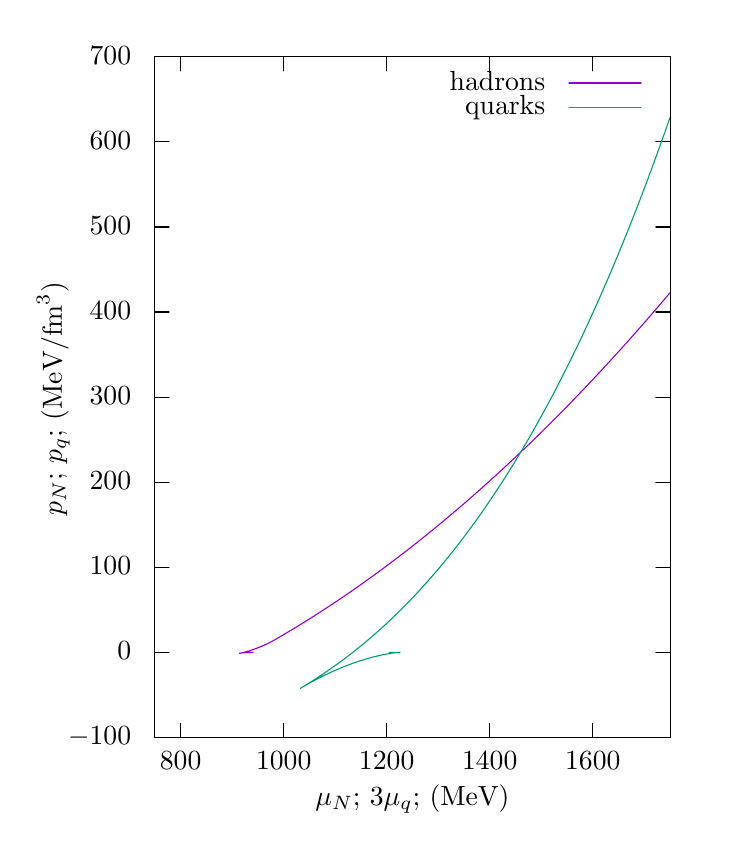
\begin{tikzpicture}[gnuplot]
%% generated with GNUPLOT 5.0p4 (Lua 5.2; terminal rev. 99, script rev. 100)
%% Thu Sep 29 16:33:17 2016
\path (0.000,0.000) rectangle (8.600,10.000);
\gpcolor{color=gp lt color border}
\gpsetlinetype{gp lt border}
\gpsetdashtype{gp dt solid}
\gpsetlinewidth{1.00}
\draw[gp path] (1.504,0.985)--(1.684,0.985);
\draw[gp path] (8.047,0.985)--(7.867,0.985);
\node[gp node right] at (1.320,0.985) {$-100$};
\draw[gp path] (1.504,2.066)--(1.684,2.066);
\draw[gp path] (8.047,2.066)--(7.867,2.066);
\node[gp node right] at (1.320,2.066) {$0$};
\draw[gp path] (1.504,3.147)--(1.684,3.147);
\draw[gp path] (8.047,3.147)--(7.867,3.147);
\node[gp node right] at (1.320,3.147) {$100$};
\draw[gp path] (1.504,4.227)--(1.684,4.227);
\draw[gp path] (8.047,4.227)--(7.867,4.227);
\node[gp node right] at (1.320,4.227) {$200$};
\draw[gp path] (1.504,5.308)--(1.684,5.308);
\draw[gp path] (8.047,5.308)--(7.867,5.308);
\node[gp node right] at (1.320,5.308) {$300$};
\draw[gp path] (1.504,6.389)--(1.684,6.389);
\draw[gp path] (8.047,6.389)--(7.867,6.389);
\node[gp node right] at (1.320,6.389) {$400$};
\draw[gp path] (1.504,7.469)--(1.684,7.469);
\draw[gp path] (8.047,7.469)--(7.867,7.469);
\node[gp node right] at (1.320,7.469) {$500$};
\draw[gp path] (1.504,8.550)--(1.684,8.550);
\draw[gp path] (8.047,8.550)--(7.867,8.550);
\node[gp node right] at (1.320,8.550) {$600$};
\draw[gp path] (1.504,9.631)--(1.684,9.631);
\draw[gp path] (8.047,9.631)--(7.867,9.631);
\node[gp node right] at (1.320,9.631) {$700$};
\draw[gp path] (1.831,0.985)--(1.831,1.165);
\draw[gp path] (1.831,9.631)--(1.831,9.451);
\node[gp node center] at (1.831,0.677) {$800$};
\draw[gp path] (3.140,0.985)--(3.140,1.165);
\draw[gp path] (3.140,9.631)--(3.140,9.451);
\node[gp node center] at (3.140,0.677) {$1000$};
\draw[gp path] (4.448,0.985)--(4.448,1.165);
\draw[gp path] (4.448,9.631)--(4.448,9.451);
\node[gp node center] at (4.448,0.677) {$1200$};
\draw[gp path] (5.757,0.985)--(5.757,1.165);
\draw[gp path] (5.757,9.631)--(5.757,9.451);
\node[gp node center] at (5.757,0.677) {$1400$};
\draw[gp path] (7.066,0.985)--(7.066,1.165);
\draw[gp path] (7.066,9.631)--(7.066,9.451);
\node[gp node center] at (7.066,0.677) {$1600$};
\draw[gp path] (1.504,9.631)--(1.504,0.985)--(8.047,0.985)--(8.047,9.631)--cycle;
\node[gp node center,rotate=-270] at (0.246,5.308) {$p_N$; $p_q$; ($\rm{MeV}/\rm{fm}^3$)};
\node[gp node center] at (4.775,0.215) {$\mu_N$; $3\mu_q$; (MeV)};
\node[gp node right] at (6.579,9.297) {hadrons};
\gpcolor{rgb color={0.580,0.000,0.827}}
\draw[gp path] (6.763,9.297)--(7.679,9.297);
\draw[gp path] (2.728,2.066)--(2.736,2.066)--(2.745,2.066)--(2.753,2.066)--(2.722,2.066)%
  --(2.730,2.066)--(2.738,2.066)--(2.745,2.066)--(2.714,2.065)--(2.722,2.066)--(2.729,2.066)%
  --(2.736,2.066)--(2.744,2.066)--(2.713,2.065)--(2.720,2.065)--(2.727,2.066)--(2.734,2.066)%
  --(2.704,2.065)--(2.711,2.065)--(2.718,2.065)--(2.725,2.066)--(2.694,2.065)--(2.701,2.065)%
  --(2.709,2.065)--(2.716,2.065)--(2.685,2.065)--(2.692,2.065)--(2.699,2.065)--(2.706,2.065)%
  --(2.713,2.065)--(2.683,2.064)--(2.690,2.065)--(2.697,2.065)--(2.704,2.065)--(2.673,2.064)%
  --(2.680,2.064)--(2.688,2.065)--(2.695,2.065)--(2.664,2.064)--(2.671,2.064)--(2.679,2.064)%
  --(2.686,2.065)--(2.693,2.065)--(2.662,2.063)--(2.670,2.064)--(2.677,2.064)--(2.684,2.065)%
  --(2.653,2.063)--(2.661,2.063)--(2.668,2.064)--(2.675,2.064)--(2.645,2.062)--(2.652,2.063)%
  --(2.659,2.063)--(2.667,2.064)--(2.674,2.064)--(2.644,2.062)--(2.651,2.063)--(2.658,2.063)%
  --(2.665,2.064)--(2.635,2.062)--(2.643,2.062)--(2.650,2.063)--(2.657,2.063)--(2.627,2.061)%
  --(2.635,2.062)--(2.642,2.062)--(2.649,2.063)--(2.657,2.063)--(2.627,2.061)--(2.634,2.061)%
  --(2.642,2.062)--(2.649,2.063)--(2.619,2.060)--(2.627,2.061)--(2.634,2.061)--(2.641,2.062)%
  --(2.612,2.060)--(2.619,2.060)--(2.627,2.061)--(2.634,2.061)--(2.642,2.062)--(2.612,2.059)%
  --(2.619,2.060)--(2.627,2.061)--(2.635,2.062)--(2.605,2.059)--(2.613,2.059)--(2.620,2.060)%
  --(2.628,2.061)--(2.598,2.058)--(2.606,2.059)--(2.613,2.060)--(2.621,2.060)--(2.629,2.061)%
  --(2.599,2.058)--(2.607,2.059)--(2.615,2.060)--(2.622,2.061)--(2.593,2.057)--(2.601,2.058)%
  --(2.609,2.059)--(2.616,2.060)--(2.624,2.061)--(2.595,2.057)--(2.603,2.058)--(2.610,2.059)%
  --(2.618,2.060)--(2.589,2.057)--(2.597,2.058)--(2.605,2.059)--(2.612,2.060)--(2.620,2.060)%
  --(2.591,2.057)--(2.599,2.058)--(2.607,2.059)--(2.615,2.060)--(2.586,2.056)--(2.594,2.057)%
  --(2.602,2.058)--(2.610,2.059)--(2.581,2.055)--(2.589,2.056)--(2.597,2.058)--(2.605,2.059)%
  --(2.613,2.060)--(2.584,2.056)--(2.592,2.057)--(2.600,2.058)--(2.608,2.059)--(2.580,2.055)%
  --(2.588,2.056)--(2.596,2.057)--(2.604,2.059)--(2.612,2.060)--(2.583,2.056)--(2.591,2.057)%
  --(2.599,2.058)--(2.607,2.059)--(2.579,2.055)--(2.587,2.056)--(2.595,2.057)--(2.603,2.059)%
  --(2.612,2.060)--(2.583,2.055)--(2.592,2.057)--(2.600,2.058)--(2.608,2.059)--(2.580,2.055)%
  --(2.588,2.056)--(2.596,2.057)--(2.604,2.059)--(2.613,2.060)--(2.585,2.056)--(2.593,2.057)%
  --(2.601,2.058)--(2.609,2.060)--(2.582,2.055)--(2.590,2.056)--(2.598,2.058)--(2.606,2.059)%
  --(2.579,2.054)--(2.587,2.056)--(2.595,2.057)--(2.604,2.059)--(2.612,2.060)--(2.585,2.055)%
  --(2.593,2.057)--(2.601,2.058)--(2.609,2.060)--(2.582,2.055)--(2.591,2.056)--(2.599,2.058)%
  --(2.607,2.060)--(2.616,2.061)--(2.588,2.056)--(2.597,2.058)--(2.605,2.059)--(2.614,2.061)%
  --(2.587,2.056)--(2.595,2.057)--(2.603,2.059)--(2.612,2.061)--(2.620,2.062)--(2.593,2.057)%
  --(2.602,2.059)--(2.610,2.060)--(2.619,2.062)--(2.592,2.056)--(2.600,2.058)--(2.609,2.060)%
  --(2.617,2.062)--(2.626,2.064)--(2.599,2.058)--(2.608,2.060)--(2.616,2.062)--(2.625,2.063)%
  --(2.598,2.058)--(2.607,2.060)--(2.616,2.061)--(2.624,2.063)--(2.598,2.057)--(2.606,2.059)%
  --(2.615,2.061)--(2.624,2.063)--(2.632,2.065)--(2.606,2.059)--(2.615,2.061)--(2.623,2.063)%
  --(2.632,2.065)--(2.606,2.059)--(2.614,2.061)--(2.623,2.063)--(2.632,2.065)--(2.640,2.067)%
  --(2.614,2.061)--(2.623,2.063)--(2.632,2.065)--(2.641,2.067)--(2.615,2.061)--(2.623,2.063)%
  --(2.632,2.065)--(2.641,2.068)--(2.615,2.061)--(2.624,2.063)--(2.633,2.066)--(2.642,2.068)%
  --(2.650,2.070)--(2.625,2.063)--(2.633,2.066)--(2.642,2.068)--(2.651,2.070)--(2.626,2.064)%
  --(2.634,2.066)--(2.643,2.068)--(2.652,2.071)--(2.661,2.073)--(2.636,2.066)--(2.645,2.069)%
  --(2.653,2.071)--(2.662,2.073)--(2.637,2.067)--(2.646,2.069)--(2.655,2.071)--(2.664,2.074)%
  --(2.639,2.067)--(2.648,2.069)--(2.657,2.072)--(2.666,2.074)--(2.675,2.077)--(2.650,2.070)%
  --(2.659,2.072)--(2.668,2.075)--(2.676,2.077)--(2.652,2.070)--(2.661,2.073)--(2.670,2.075)%
  --(2.679,2.078)--(2.654,2.071)--(2.663,2.074)--(2.672,2.076)--(2.681,2.079)--(2.690,2.081)%
  --(2.674,2.077)--(2.683,2.079)--(2.675,2.077)--(2.684,2.080)--(2.677,2.078)--(2.686,2.080)%
  --(2.678,2.078)--(2.687,2.081)--(2.680,2.078)--(2.689,2.081)--(2.681,2.079)--(2.690,2.082)%
  --(2.683,2.079)--(2.692,2.082)--(2.685,2.080)--(2.694,2.083)--(2.703,2.085)--(2.696,2.083)%
  --(2.705,2.086)--(2.697,2.084)--(2.707,2.087)--(2.699,2.084)--(2.708,2.087)--(2.701,2.085)%
  --(2.710,2.088)--(2.703,2.086)--(2.712,2.088)--(2.705,2.086)--(2.714,2.089)--(2.707,2.087)%
  --(2.716,2.090)--(2.709,2.088)--(2.719,2.091)--(2.712,2.088)--(2.721,2.091)--(2.714,2.089)%
  --(2.723,2.092)--(2.716,2.090)--(2.725,2.093)--(2.735,2.096)--(2.728,2.094)--(2.737,2.097)%
  --(2.730,2.094)--(2.739,2.097)--(2.733,2.095)--(2.742,2.098)--(2.735,2.096)--(2.744,2.099)%
  --(2.738,2.097)--(2.747,2.100)--(2.740,2.098)--(2.750,2.101)--(2.743,2.099)--(2.752,2.102)%
  --(2.746,2.100)--(2.755,2.103)--(2.749,2.101)--(2.758,2.104)--(2.752,2.102)--(2.761,2.105)%
  --(2.755,2.103)--(2.764,2.106)--(2.757,2.104)--(2.767,2.107)--(2.761,2.105)--(2.770,2.108)%
  --(2.764,2.106)--(2.773,2.109)--(2.767,2.107)--(2.776,2.111)--(2.770,2.108)--(2.779,2.112)%
  --(2.773,2.110)--(2.783,2.113)--(2.777,2.111)--(2.786,2.114)--(2.780,2.112)--(2.789,2.116)%
  --(2.783,2.113)--(2.793,2.117)--(2.787,2.115)--(2.796,2.118)--(2.790,2.116)--(2.800,2.120)%
  --(2.794,2.117)--(2.803,2.121)--(2.798,2.119)--(2.807,2.122)--(2.801,2.120)--(2.796,2.118)%
  --(2.805,2.122)--(2.800,2.119)--(2.809,2.123)--(2.804,2.121)--(2.813,2.125)--(2.807,2.123)%
  --(2.817,2.126)--(2.811,2.124)--(2.821,2.128)--(2.816,2.126)--(2.825,2.130)--(2.820,2.127)%
  --(2.829,2.131)--(2.824,2.129)--(2.833,2.133)--(2.828,2.131)--(2.823,2.129)--(2.832,2.133)%
  --(2.827,2.130)--(2.837,2.134)--(2.832,2.132)--(2.841,2.136)--(2.836,2.134)--(2.846,2.138)%
  --(2.841,2.136)--(2.850,2.140)--(2.845,2.138)--(2.855,2.142)--(2.850,2.140)--(2.845,2.138)%
  --(2.855,2.142)--(2.850,2.140)--(2.859,2.144)--(2.855,2.142)--(2.864,2.146)--(2.860,2.144)%
  --(2.855,2.142)--(2.865,2.146)--(2.860,2.144)--(2.870,2.148)--(2.865,2.146)--(2.875,2.151)%
  --(2.870,2.149)--(2.880,2.153)--(2.876,2.151)--(2.871,2.149)--(2.881,2.153)--(2.877,2.151)%
  --(2.886,2.156)--(2.882,2.154)--(2.878,2.152)--(2.888,2.156)--(2.884,2.154)--(2.893,2.159)%
  --(2.889,2.157)--(2.899,2.161)--(2.895,2.159)--(2.891,2.158)--(2.901,2.162)--(2.897,2.160)%
  --(2.906,2.165)--(2.903,2.163)--(2.899,2.161)--(2.909,2.166)--(2.905,2.164)--(2.901,2.162)%
  --(2.911,2.167)--(2.908,2.165)--(2.917,2.170)--(2.914,2.168)--(2.910,2.167)--(2.920,2.171)%
  --(2.917,2.170)--(2.926,2.174)--(2.923,2.173)--(2.920,2.171)--(2.930,2.176)--(2.927,2.174)%
  --(2.924,2.173)--(2.933,2.177)--(2.930,2.176)--(2.928,2.175)--(2.937,2.179)--(2.934,2.178)%
  --(2.932,2.177)--(2.941,2.181)--(2.939,2.180)--(2.936,2.179)--(2.946,2.183)--(2.943,2.182)%
  --(2.941,2.181)--(2.950,2.186)--(2.948,2.185)--(2.946,2.184)--(2.956,2.188)--(2.950,2.186)%
  --(2.954,2.188)--(2.958,2.190)--(2.956,2.189)--(2.960,2.190)--(2.958,2.190)--(2.962,2.191)%
  --(2.960,2.191)--(2.964,2.193)--(2.963,2.192)--(2.967,2.194)--(2.971,2.196)--(2.969,2.195)%
  --(2.973,2.197)--(2.972,2.197)--(2.976,2.199)--(2.975,2.198)--(2.974,2.198)--(2.978,2.200)%
  --(2.977,2.199)--(2.981,2.201)--(2.985,2.203)--(2.984,2.203)--(2.988,2.205)--(2.987,2.205)%
  --(2.992,2.207)--(2.996,2.209)--(2.997,2.209)--(3.002,2.212)--(3.003,2.213)--(3.004,2.213)%
  --(3.004,2.214)--(3.005,2.214)--(3.006,2.215)--(3.007,2.215)--(3.008,2.216)--(3.010,2.216)%
  --(3.011,2.217)--(3.013,2.218)--(3.014,2.219)--(3.016,2.220)--(3.018,2.221)--(3.020,2.222)%
  --(3.018,2.221)--(3.020,2.222)--(3.023,2.224)--(3.022,2.223)--(3.024,2.224)--(3.025,2.225)%
  --(3.026,2.225)--(3.027,2.226)--(3.029,2.227)--(3.030,2.228)--(3.031,2.228)--(3.032,2.229)%
  --(3.034,2.230)--(3.036,2.231)--(3.038,2.232)--(3.040,2.233)--(3.041,2.234)--(3.042,2.234)%
  --(3.042,2.235)--(3.043,2.235)--(3.044,2.236)--(3.047,2.237)--(3.056,2.243)--(3.066,2.248)%
  --(3.075,2.254)--(3.084,2.259)--(3.094,2.265)--(3.103,2.270)--(3.113,2.276)--(3.122,2.281)%
  --(3.131,2.287)--(3.141,2.292)--(3.150,2.298)--(3.160,2.303)--(3.169,2.309)--(3.178,2.315)%
  --(3.188,2.320)--(3.197,2.326)--(3.207,2.331)--(3.216,2.337)--(3.225,2.343)--(3.235,2.348)%
  --(3.244,2.354)--(3.254,2.360)--(3.263,2.365)--(3.272,2.371)--(3.282,2.377)--(3.291,2.382)%
  --(3.300,2.388)--(3.310,2.394)--(3.319,2.399)--(3.329,2.405)--(3.338,2.411)--(3.347,2.417)%
  --(3.357,2.422)--(3.366,2.428)--(3.375,2.434)--(3.385,2.440)--(3.394,2.446)--(3.403,2.451)%
  --(3.413,2.457)--(3.422,2.463)--(3.432,2.469)--(3.441,2.475)--(3.450,2.481)--(3.460,2.486)%
  --(3.469,2.492)--(3.478,2.498)--(3.488,2.504)--(3.497,2.510)--(3.506,2.516)--(3.516,2.522)%
  --(3.525,2.528)--(3.534,2.534)--(3.544,2.540)--(3.553,2.546)--(3.562,2.552)--(3.572,2.558)%
  --(3.581,2.564)--(3.590,2.570)--(3.600,2.576)--(3.609,2.582)--(3.618,2.588)--(3.628,2.594)%
  --(3.637,2.600)--(3.646,2.606)--(3.655,2.612)--(3.665,2.618)--(3.674,2.624)--(3.683,2.630)%
  --(3.693,2.636)--(3.702,2.642)--(3.711,2.648)--(3.721,2.654)--(3.730,2.661)--(3.739,2.667)%
  --(3.749,2.673)--(3.758,2.679)--(3.767,2.685)--(3.776,2.691)--(3.786,2.698)--(3.795,2.704)%
  --(3.804,2.710)--(3.814,2.716)--(3.823,2.722)--(3.832,2.729)--(3.841,2.735)--(3.851,2.741)%
  --(3.860,2.747)--(3.869,2.754)--(3.879,2.760)--(3.888,2.766)--(3.897,2.773)--(3.906,2.779)%
  --(3.916,2.785)--(3.925,2.792)--(3.934,2.798)--(3.943,2.804)--(3.953,2.811)--(3.962,2.817)%
  --(3.971,2.823)--(3.981,2.830)--(3.990,2.836)--(3.999,2.843)--(4.008,2.849)--(4.018,2.855)%
  --(4.027,2.862)--(4.036,2.868)--(4.045,2.875)--(4.055,2.881)--(4.064,2.888)--(4.073,2.894)%
  --(4.082,2.901)--(4.092,2.907)--(4.101,2.914)--(4.110,2.920)--(4.119,2.927)--(4.129,2.933)%
  --(4.138,2.940)--(4.147,2.946)--(4.156,2.953)--(4.166,2.959)--(4.175,2.966)--(4.184,2.973)%
  --(4.193,2.979)--(4.203,2.986)--(4.212,2.992)--(4.221,2.999)--(4.230,3.006)--(4.239,3.012)%
  --(4.249,3.019)--(4.258,3.026)--(4.267,3.032)--(4.276,3.039)--(4.286,3.046)--(4.295,3.052)%
  --(4.304,3.059)--(4.313,3.066)--(4.322,3.073)--(4.332,3.079)--(4.341,3.086)--(4.350,3.093)%
  --(4.359,3.100)--(4.369,3.106)--(4.378,3.113)--(4.387,3.120)--(4.396,3.127)--(4.405,3.134)%
  --(4.415,3.140)--(4.424,3.147)--(4.433,3.154)--(4.442,3.161)--(4.451,3.168)--(4.461,3.175)%
  --(4.470,3.181)--(4.479,3.188)--(4.488,3.195)--(4.497,3.202)--(4.507,3.209)--(4.516,3.216)%
  --(4.525,3.223)--(4.534,3.230)--(4.543,3.237)--(4.553,3.244)--(4.562,3.251)--(4.571,3.258)%
  --(4.580,3.265)--(4.589,3.272)--(4.598,3.279)--(4.608,3.286)--(4.617,3.293)--(4.626,3.300)%
  --(4.635,3.307)--(4.644,3.314)--(4.653,3.321)--(4.663,3.328)--(4.672,3.335)--(4.681,3.342)%
  --(4.690,3.349)--(4.699,3.356)--(4.709,3.363)--(4.718,3.371)--(4.727,3.378)--(4.736,3.385)%
  --(4.745,3.392)--(4.754,3.399)--(4.764,3.406)--(4.773,3.414)--(4.782,3.421)--(4.791,3.428)%
  --(4.800,3.435)--(4.809,3.442)--(4.818,3.450)--(4.828,3.457)--(4.837,3.464)--(4.846,3.471)%
  --(4.855,3.479)--(4.864,3.486)--(4.873,3.493)--(4.883,3.500)--(4.892,3.508)--(4.901,3.515)%
  --(4.910,3.522)--(4.919,3.530)--(4.928,3.537)--(4.937,3.544)--(4.947,3.552)--(4.956,3.559)%
  --(4.965,3.567)--(4.974,3.574)--(4.983,3.581)--(4.992,3.589)--(5.001,3.596)--(5.010,3.604)%
  --(5.020,3.611)--(5.029,3.618)--(5.038,3.626)--(5.047,3.633)--(5.056,3.641)--(5.065,3.648)%
  --(5.074,3.656)--(5.084,3.663)--(5.093,3.671)--(5.102,3.678)--(5.111,3.686)--(5.120,3.693)%
  --(5.129,3.701)--(5.138,3.708)--(5.147,3.716)--(5.157,3.724)--(5.166,3.731)--(5.175,3.739)%
  --(5.184,3.746)--(5.193,3.754)--(5.202,3.762)--(5.211,3.769)--(5.220,3.777)--(5.229,3.784)%
  --(5.239,3.792)--(5.248,3.800)--(5.257,3.807)--(5.266,3.815)--(5.275,3.823)--(5.284,3.830)%
  --(5.293,3.838)--(5.302,3.846)--(5.311,3.854)--(5.320,3.861)--(5.330,3.869)--(5.339,3.877)%
  --(5.348,3.885)--(5.357,3.892)--(5.366,3.900)--(5.375,3.908)--(5.384,3.916)--(5.393,3.924)%
  --(5.402,3.931)--(5.411,3.939)--(5.420,3.947)--(5.430,3.955)--(5.439,3.963)--(5.448,3.971)%
  --(5.457,3.978)--(5.466,3.986)--(5.475,3.994)--(5.484,4.002)--(5.493,4.010)--(5.502,4.018)%
  --(5.511,4.026)--(5.520,4.034)--(5.530,4.042)--(5.539,4.050)--(5.548,4.058)--(5.557,4.066)%
  --(5.566,4.074)--(5.575,4.082)--(5.584,4.090)--(5.593,4.098)--(5.602,4.106)--(5.611,4.114)%
  --(5.620,4.122)--(5.629,4.130)--(5.638,4.138)--(5.647,4.146)--(5.657,4.154)--(5.666,4.162)%
  --(5.675,4.170)--(5.684,4.178)--(5.693,4.186)--(5.702,4.195)--(5.711,4.203)--(5.720,4.211)%
  --(5.729,4.219)--(5.738,4.227)--(5.747,4.235)--(5.756,4.243)--(5.765,4.252)--(5.774,4.260)%
  --(5.783,4.268)--(5.792,4.276)--(5.801,4.284)--(5.811,4.293)--(5.820,4.301)--(5.829,4.309)%
  --(5.838,4.317)--(5.847,4.326)--(5.856,4.334)--(5.865,4.342)--(5.874,4.351)--(5.883,4.359)%
  --(5.892,4.367)--(5.901,4.376)--(5.910,4.384)--(5.919,4.392)--(5.928,4.401)--(5.937,4.409)%
  --(5.946,4.417)--(5.955,4.426)--(5.964,4.434)--(5.973,4.442)--(5.982,4.451)--(5.991,4.459)%
  --(6.000,4.468)--(6.009,4.476)--(6.018,4.485)--(6.028,4.493)--(6.037,4.502)--(6.046,4.510)%
  --(6.055,4.518)--(6.064,4.527)--(6.073,4.535)--(6.082,4.544)--(6.091,4.552)--(6.100,4.561)%
  --(6.109,4.570)--(6.118,4.578)--(6.127,4.587)--(6.136,4.595)--(6.145,4.604)--(6.154,4.612)%
  --(6.163,4.621)--(6.172,4.630)--(6.181,4.638)--(6.190,4.647)--(6.199,4.655)--(6.208,4.664)%
  --(6.217,4.673)--(6.226,4.681)--(6.235,4.690)--(6.244,4.699)--(6.253,4.707)--(6.262,4.716)%
  --(6.271,4.725)--(6.280,4.733)--(6.289,4.742)--(6.298,4.751)--(6.307,4.760)--(6.316,4.768)%
  --(6.325,4.777)--(6.334,4.786)--(6.343,4.795)--(6.352,4.803)--(6.361,4.812)--(6.370,4.821)%
  --(6.379,4.830)--(6.388,4.839)--(6.397,4.848)--(6.406,4.856)--(6.415,4.865)--(6.424,4.874)%
  --(6.433,4.883)--(6.442,4.892)--(6.451,4.901)--(6.460,4.910)--(6.469,4.918)--(6.478,4.927)%
  --(6.487,4.936)--(6.496,4.945)--(6.505,4.954)--(6.514,4.963)--(6.523,4.972)--(6.532,4.981)%
  --(6.541,4.990)--(6.550,4.999)--(6.559,5.008)--(6.568,5.017)--(6.577,5.026)--(6.586,5.035)%
  --(6.595,5.044)--(6.604,5.053)--(6.613,5.062)--(6.622,5.071)--(6.631,5.080)--(6.640,5.089)%
  --(6.649,5.098)--(6.658,5.108)--(6.667,5.117)--(6.676,5.126)--(6.685,5.135)--(6.694,5.144)%
  --(6.703,5.153)--(6.712,5.162)--(6.721,5.171)--(6.730,5.181)--(6.739,5.190)--(6.748,5.199)%
  --(6.757,5.208)--(6.766,5.217)--(6.775,5.227)--(6.784,5.236)--(6.792,5.245)--(6.801,5.254)%
  --(6.810,5.264)--(6.819,5.273)--(6.828,5.282)--(6.837,5.291)--(6.846,5.301)--(6.855,5.310)%
  --(6.864,5.319)--(6.873,5.329)--(6.882,5.338)--(6.891,5.347)--(6.900,5.357)--(6.909,5.366)%
  --(6.918,5.375)--(6.927,5.385)--(6.936,5.394)--(6.945,5.403)--(6.954,5.413)--(6.963,5.422)%
  --(6.972,5.432)--(6.981,5.441)--(6.990,5.451)--(6.999,5.460)--(7.008,5.469)--(7.016,5.479)%
  --(7.025,5.488)--(7.034,5.498)--(7.043,5.507)--(7.052,5.517)--(7.061,5.526)--(7.070,5.536)%
  --(7.079,5.545)--(7.088,5.555)--(7.097,5.564)--(7.106,5.574)--(7.115,5.584)--(7.124,5.593)%
  --(7.133,5.603)--(7.142,5.612)--(7.151,5.622)--(7.160,5.632)--(7.169,5.641)--(7.177,5.651)%
  --(7.186,5.660)--(7.195,5.670)--(7.204,5.680)--(7.213,5.689)--(7.222,5.699)--(7.231,5.709)%
  --(7.240,5.718)--(7.249,5.728)--(7.258,5.738)--(7.267,5.748)--(7.276,5.757)--(7.285,5.767)%
  --(7.294,5.777)--(7.303,5.787)--(7.312,5.796)--(7.320,5.806)--(7.329,5.816)--(7.338,5.826)%
  --(7.347,5.835)--(7.356,5.845)--(7.365,5.855)--(7.374,5.865)--(7.383,5.875)--(7.392,5.885)%
  --(7.401,5.894)--(7.410,5.904)--(7.419,5.914)--(7.428,5.924)--(7.436,5.934)--(7.445,5.944)%
  --(7.454,5.954)--(7.463,5.964)--(7.472,5.974)--(7.481,5.984)--(7.490,5.993)--(7.499,6.003)%
  --(7.508,6.013)--(7.517,6.023)--(7.526,6.033)--(7.535,6.043)--(7.544,6.053)--(7.552,6.063)%
  --(7.561,6.073)--(7.570,6.083)--(7.579,6.093)--(7.588,6.103)--(7.597,6.114)--(7.606,6.124)%
  --(7.615,6.134)--(7.624,6.144)--(7.633,6.154)--(7.642,6.164)--(7.650,6.174)--(7.659,6.184)%
  --(7.668,6.194)--(7.677,6.204)--(7.686,6.215)--(7.695,6.225)--(7.704,6.235)--(7.713,6.245)%
  --(7.722,6.255)--(7.731,6.265)--(7.740,6.276)--(7.748,6.286)--(7.757,6.296)--(7.766,6.306)%
  --(7.775,6.317)--(7.784,6.327)--(7.793,6.337)--(7.802,6.347)--(7.811,6.358)--(7.820,6.368)%
  --(7.828,6.378)--(7.837,6.389)--(7.846,6.399)--(7.855,6.409)--(7.864,6.420)--(7.873,6.430)%
  --(7.882,6.440)--(7.891,6.451)--(7.900,6.461)--(7.909,6.471)--(7.917,6.482)--(7.926,6.492)%
  --(7.935,6.502)--(7.944,6.513)--(7.953,6.523)--(7.962,6.534)--(7.971,6.544)--(7.980,6.555)%
  --(7.989,6.565)--(7.997,6.576)--(8.006,6.586)--(8.015,6.597)--(8.024,6.607)--(8.033,6.618)%
  --(8.042,6.628)--(8.047,6.634);
\gpcolor{color=gp lt color border}
\node[gp node right] at (6.579,8.989) {quarks};
\gpcolor{rgb color={0.000,0.620,0.451}}
\draw[gp path] (6.763,8.989)--(7.679,8.989);
\draw[gp path] (4.480,2.066)--(4.513,2.066)--(4.535,2.066)--(4.551,2.066)--(4.564,2.066)%
  --(4.575,2.066)--(4.583,2.067)--(4.591,2.067)--(4.597,2.067)--(4.601,2.067)--(4.606,2.067)%
  --(4.609,2.067)--(4.612,2.067)--(4.614,2.067)--(4.616,2.068)--(4.617,2.068)--(4.618,2.068)%
  --(4.617,2.068)--(4.616,2.068)--(4.615,2.067)--(4.614,2.067)--(4.613,2.067)--(4.611,2.067)%
  --(4.609,2.067)--(4.607,2.067)--(4.604,2.067)--(4.602,2.066)--(4.599,2.066)--(4.596,2.066)%
  --(4.593,2.066)--(4.589,2.065)--(4.586,2.065)--(4.583,2.065)--(4.579,2.064)--(4.575,2.064)%
  --(4.571,2.063)--(4.567,2.063)--(4.563,2.063)--(4.559,2.062)--(4.554,2.061)--(4.550,2.061)%
  --(4.545,2.060)--(4.540,2.060)--(4.536,2.059)--(4.531,2.058)--(4.526,2.058)--(4.521,2.057)%
  --(4.516,2.056)--(4.511,2.056)--(4.505,2.055)--(4.500,2.054)--(4.495,2.053)--(4.489,2.052)%
  --(4.483,2.051)--(4.478,2.050)--(4.472,2.049)--(4.466,2.048)--(4.460,2.047)--(4.455,2.046)%
  --(4.449,2.045)--(4.443,2.044)--(4.437,2.043)--(4.431,2.042)--(4.424,2.041)--(4.418,2.040)%
  --(4.412,2.038)--(4.406,2.037)--(4.399,2.036)--(4.393,2.035)--(4.386,2.033)--(4.380,2.032)%
  --(4.373,2.030)--(4.367,2.029)--(4.360,2.027)--(4.354,2.026)--(4.347,2.024)--(4.340,2.023)%
  --(4.333,2.021)--(4.327,2.020)--(4.320,2.018)--(4.313,2.016)--(4.306,2.015)--(4.299,2.013)%
  --(4.292,2.011)--(4.285,2.010)--(4.278,2.008)--(4.271,2.006)--(4.264,2.004)--(4.257,2.002)%
  --(4.249,2.000)--(4.242,1.998)--(4.235,1.996)--(4.228,1.994)--(4.220,1.992)--(4.213,1.990)%
  --(4.206,1.988)--(4.198,1.986)--(4.191,1.984)--(4.183,1.982)--(4.176,1.979)--(4.169,1.977)%
  --(4.161,1.975)--(4.153,1.972)--(4.146,1.970)--(4.138,1.968)--(4.131,1.965)--(4.123,1.963)%
  --(4.115,1.960)--(4.108,1.958)--(4.100,1.956)--(4.092,1.953)--(4.084,1.950)--(4.077,1.948)%
  --(4.069,1.945)--(4.061,1.942)--(4.053,1.940)--(4.045,1.937)--(4.038,1.934)--(4.030,1.931)%
  --(4.022,1.929)--(4.014,1.926)--(4.006,1.923)--(3.998,1.920)--(3.990,1.917)--(3.982,1.914)%
  --(3.974,1.911)--(3.966,1.908)--(3.958,1.905)--(3.950,1.902)--(3.942,1.899)--(3.933,1.896)%
  --(3.925,1.892)--(3.917,1.889)--(3.909,1.886)--(3.901,1.883)--(3.893,1.879)--(3.884,1.876)%
  --(3.876,1.873)--(3.868,1.869)--(3.860,1.866)--(3.851,1.862)--(3.843,1.859)--(3.835,1.855)%
  --(3.827,1.852)--(3.818,1.848)--(3.810,1.845)--(3.802,1.841)--(3.793,1.837)--(3.785,1.834)%
  --(3.776,1.830)--(3.768,1.826)--(3.760,1.822)--(3.751,1.819)--(3.743,1.815)--(3.734,1.811)%
  --(3.726,1.807)--(3.717,1.803)--(3.709,1.799)--(3.700,1.795)--(3.692,1.791)--(3.683,1.787)%
  --(3.675,1.783)--(3.666,1.779)--(3.657,1.775)--(3.649,1.770)--(3.640,1.766)--(3.632,1.762)%
  --(3.623,1.758)--(3.614,1.753)--(3.606,1.749)--(3.597,1.744)--(3.588,1.740)--(3.580,1.736)%
  --(3.571,1.731)--(3.562,1.727)--(3.554,1.722)--(3.545,1.718)--(3.536,1.713)--(3.527,1.708)%
  --(3.519,1.704)--(3.510,1.699)--(3.501,1.694)--(3.492,1.690)--(3.484,1.685)--(3.475,1.680)%
  --(3.466,1.675)--(3.457,1.670)--(3.448,1.665)--(3.439,1.660)--(3.431,1.655)--(3.422,1.650)%
  --(3.413,1.645)--(3.404,1.640)--(3.395,1.635)--(3.386,1.630)--(3.377,1.625)--(3.368,1.620)%
  --(3.360,1.614)--(3.351,1.609)--(3.356,1.612)--(3.367,1.619)--(3.378,1.626)--(3.389,1.632)%
  --(3.400,1.639)--(3.411,1.646)--(3.422,1.652)--(3.433,1.659)--(3.444,1.666)--(3.455,1.672)%
  --(3.466,1.679)--(3.477,1.686)--(3.487,1.693)--(3.498,1.699)--(3.509,1.706)--(3.519,1.713)%
  --(3.530,1.720)--(3.541,1.727)--(3.551,1.733)--(3.562,1.740)--(3.572,1.747)--(3.583,1.754)%
  --(3.593,1.761)--(3.604,1.768)--(3.614,1.774)--(3.624,1.781)--(3.635,1.788)--(3.645,1.795)%
  --(3.655,1.802)--(3.666,1.809)--(3.676,1.816)--(3.686,1.823)--(3.696,1.830)--(3.706,1.837)%
  --(3.716,1.844)--(3.726,1.851)--(3.736,1.858)--(3.746,1.865)--(3.756,1.872)--(3.766,1.879)%
  --(3.776,1.886)--(3.786,1.893)--(3.796,1.900)--(3.806,1.907)--(3.816,1.914)--(3.825,1.921)%
  --(3.835,1.928)--(3.845,1.935)--(3.855,1.942)--(3.864,1.950)--(3.874,1.957)--(3.884,1.964)%
  --(3.893,1.971)--(3.903,1.978)--(3.912,1.985)--(3.922,1.992)--(3.931,2.000)--(3.941,2.007)%
  --(3.950,2.014)--(3.960,2.021)--(3.969,2.028)--(3.979,2.036)--(3.988,2.043)--(3.997,2.050)%
  --(4.007,2.057)--(4.016,2.065)--(4.025,2.072)--(4.034,2.079)--(4.044,2.087)--(4.053,2.094)%
  --(4.062,2.101)--(4.071,2.109)--(4.080,2.116)--(4.089,2.123)--(4.098,2.131)--(4.107,2.138)%
  --(4.116,2.145)--(4.126,2.153)--(4.135,2.160)--(4.143,2.167)--(4.152,2.175)--(4.161,2.182)%
  --(4.170,2.190)--(4.179,2.197)--(4.188,2.205)--(4.197,2.212)--(4.206,2.219)--(4.215,2.227)%
  --(4.223,2.234)--(4.232,2.242)--(4.241,2.249)--(4.250,2.257)--(4.258,2.264)--(4.267,2.272)%
  --(4.276,2.279)--(4.284,2.287)--(4.293,2.294)--(4.302,2.302)--(4.310,2.310)--(4.319,2.317)%
  --(4.327,2.325)--(4.336,2.332)--(4.344,2.340)--(4.353,2.348)--(4.361,2.355)--(4.370,2.363)%
  --(4.378,2.370)--(4.387,2.378)--(4.395,2.386)--(4.403,2.393)--(4.412,2.401)--(4.420,2.409)%
  --(4.428,2.416)--(4.437,2.424)--(4.445,2.432)--(4.453,2.439)--(4.462,2.447)--(4.470,2.455)%
  --(4.478,2.463)--(4.486,2.470)--(4.495,2.478)--(4.503,2.486)--(4.511,2.493)--(4.519,2.501)%
  --(4.527,2.509)--(4.535,2.517)--(4.543,2.525)--(4.551,2.532)--(4.559,2.540)--(4.568,2.548)%
  --(4.576,2.556)--(4.584,2.564)--(4.592,2.571)--(4.600,2.579)--(4.608,2.587)--(4.615,2.595)%
  --(4.623,2.603)--(4.631,2.611)--(4.639,2.619)--(4.647,2.627)--(4.655,2.634)--(4.663,2.642)%
  --(4.671,2.650)--(4.678,2.658)--(4.686,2.666)--(4.694,2.674)--(4.702,2.682)--(4.710,2.690)%
  --(4.717,2.698)--(4.725,2.706)--(4.733,2.714)--(4.741,2.722)--(4.748,2.730)--(4.756,2.738)%
  --(4.764,2.746)--(4.771,2.754)--(4.779,2.762)--(4.787,2.770)--(4.794,2.778)--(4.802,2.786)%
  --(4.809,2.794)--(4.817,2.802)--(4.824,2.810)--(4.832,2.818)--(4.839,2.826)--(4.847,2.834)%
  --(4.854,2.842)--(4.862,2.851)--(4.869,2.859)--(4.877,2.867)--(4.884,2.875)--(4.892,2.883)%
  --(4.899,2.891)--(4.907,2.899)--(4.914,2.907)--(4.921,2.916)--(4.929,2.924)--(4.936,2.932)%
  --(4.943,2.940)--(4.951,2.948)--(4.958,2.956)--(4.965,2.965)--(4.973,2.973)--(4.980,2.981)%
  --(4.987,2.989)--(4.994,2.998)--(5.002,3.006)--(5.009,3.014)--(5.016,3.022)--(5.023,3.031)%
  --(5.030,3.039)--(5.038,3.047)--(5.045,3.055)--(5.052,3.064)--(5.059,3.072)--(5.066,3.080)%
  --(5.073,3.089)--(5.080,3.097)--(5.087,3.105)--(5.095,3.114)--(5.102,3.122)--(5.109,3.130)%
  --(5.116,3.139)--(5.123,3.147)--(5.130,3.155)--(5.137,3.164)--(5.144,3.172)--(5.151,3.180)%
  --(5.158,3.189)--(5.165,3.197)--(5.172,3.206)--(5.179,3.214)--(5.185,3.222)--(5.192,3.231)%
  --(5.199,3.239)--(5.206,3.248)--(5.213,3.256)--(5.220,3.265)--(5.227,3.273)--(5.234,3.282)%
  --(5.241,3.290)--(5.247,3.298)--(5.254,3.307)--(5.261,3.315)--(5.268,3.324)--(5.275,3.332)%
  --(5.281,3.341)--(5.288,3.350)--(5.295,3.358)--(5.302,3.367)--(5.308,3.375)--(5.315,3.384)%
  --(5.322,3.392)--(5.328,3.401)--(5.335,3.409)--(5.342,3.418)--(5.349,3.426)--(5.355,3.435)%
  --(5.362,3.444)--(5.368,3.452)--(5.375,3.461)--(5.382,3.469)--(5.388,3.478)--(5.395,3.487)%
  --(5.402,3.495)--(5.408,3.504)--(5.415,3.513)--(5.421,3.521)--(5.428,3.530)--(5.434,3.539)%
  --(5.441,3.547)--(5.447,3.556)--(5.454,3.565)--(5.460,3.573)--(5.467,3.582)--(5.473,3.591)%
  --(5.480,3.599)--(5.486,3.608)--(5.493,3.617)--(5.499,3.626)--(5.506,3.634)--(5.512,3.643)%
  --(5.519,3.652)--(5.525,3.661)--(5.531,3.669)--(5.538,3.678)--(5.544,3.687)--(5.551,3.696)%
  --(5.557,3.704)--(5.563,3.713)--(5.570,3.722)--(5.576,3.731)--(5.582,3.740)--(5.589,3.748)%
  --(5.595,3.757)--(5.601,3.766)--(5.607,3.775)--(5.614,3.784)--(5.620,3.793)--(5.626,3.801)%
  --(5.633,3.810)--(5.639,3.819)--(5.645,3.828)--(5.651,3.837)--(5.658,3.846)--(5.664,3.855)%
  --(5.670,3.863)--(5.676,3.872)--(5.682,3.881)--(5.688,3.890)--(5.695,3.899)--(5.701,3.908)%
  --(5.707,3.917)--(5.713,3.926)--(5.719,3.935)--(5.725,3.944)--(5.732,3.953)--(5.738,3.962)%
  --(5.744,3.971)--(5.750,3.980)--(5.756,3.989)--(5.762,3.998)--(5.768,4.007)--(5.774,4.016)%
  --(5.780,4.025)--(5.786,4.034)--(5.792,4.043)--(5.798,4.052)--(5.804,4.061)--(5.810,4.070)%
  --(5.816,4.079)--(5.822,4.088)--(5.828,4.097)--(5.834,4.106)--(5.840,4.115)--(5.846,4.124)%
  --(5.852,4.133)--(5.858,4.142)--(5.864,4.151)--(5.870,4.160)--(5.876,4.169)--(5.882,4.179)%
  --(5.888,4.188)--(5.894,4.197)--(5.900,4.206)--(5.906,4.215)--(5.912,4.224)--(5.917,4.233)%
  --(5.923,4.242)--(5.929,4.252)--(5.935,4.261)--(5.941,4.270)--(5.947,4.279)--(5.953,4.288)%
  --(5.958,4.297)--(5.964,4.307)--(5.970,4.316)--(5.976,4.325)--(5.982,4.334)--(5.987,4.343)%
  --(5.993,4.353)--(5.999,4.362)--(6.005,4.371)--(6.011,4.380)--(6.016,4.389)--(6.022,4.399)%
  --(6.028,4.408)--(6.034,4.417)--(6.039,4.426)--(6.045,4.436)--(6.051,4.445)--(6.056,4.454)%
  --(6.062,4.463)--(6.068,4.473)--(6.074,4.482)--(6.079,4.491)--(6.085,4.501)--(6.091,4.510)%
  --(6.096,4.519)--(6.102,4.529)--(6.108,4.538)--(6.113,4.547)--(6.119,4.557)--(6.124,4.566)%
  --(6.130,4.575)--(6.136,4.585)--(6.141,4.594)--(6.147,4.603)--(6.152,4.613)--(6.158,4.622)%
  --(6.164,4.631)--(6.169,4.641)--(6.175,4.650)--(6.180,4.660)--(6.186,4.669)--(6.191,4.678)%
  --(6.197,4.688)--(6.203,4.697)--(6.208,4.707)--(6.214,4.716)--(6.219,4.726)--(6.225,4.735)%
  --(6.230,4.744)--(6.236,4.754)--(6.241,4.763)--(6.247,4.773)--(6.252,4.782)--(6.258,4.792)%
  --(6.263,4.801)--(6.268,4.811)--(6.274,4.820)--(6.279,4.830)--(6.285,4.839)--(6.290,4.849)%
  --(6.296,4.858)--(6.301,4.868)--(6.307,4.877)--(6.312,4.887)--(6.317,4.896)--(6.323,4.906)%
  --(6.328,4.915)--(6.334,4.925)--(6.339,4.934)--(6.344,4.944)--(6.350,4.953)--(6.355,4.963)%
  --(6.360,4.973)--(6.366,4.982)--(6.371,4.992)--(6.376,5.001)--(6.382,5.011)--(6.387,5.021)%
  --(6.392,5.030)--(6.398,5.040)--(6.403,5.049)--(6.408,5.059)--(6.414,5.069)--(6.419,5.078)%
  --(6.424,5.088)--(6.430,5.098)--(6.435,5.107)--(6.440,5.117)--(6.445,5.126)--(6.451,5.136)%
  --(6.456,5.146)--(6.461,5.155)--(6.466,5.165)--(6.472,5.175)--(6.477,5.184)--(6.482,5.194)%
  --(6.487,5.204)--(6.493,5.214)--(6.498,5.223)--(6.503,5.233)--(6.508,5.243)--(6.513,5.252)%
  --(6.519,5.262)--(6.524,5.272)--(6.529,5.282)--(6.534,5.291)--(6.539,5.301)--(6.544,5.311)%
  --(6.550,5.321)--(6.555,5.330)--(6.560,5.340)--(6.565,5.350)--(6.570,5.360)--(6.575,5.369)%
  --(6.580,5.379)--(6.586,5.389)--(6.591,5.399)--(6.596,5.409)--(6.601,5.418)--(6.606,5.428)%
  --(6.611,5.438)--(6.616,5.448)--(6.621,5.458)--(6.626,5.468)--(6.631,5.477)--(6.636,5.487)%
  --(6.642,5.497)--(6.647,5.507)--(6.652,5.517)--(6.657,5.527)--(6.662,5.537)--(6.667,5.546)%
  --(6.672,5.556)--(6.677,5.566)--(6.682,5.576)--(6.687,5.586)--(6.692,5.596)--(6.697,5.606)%
  --(6.702,5.616)--(6.707,5.626)--(6.712,5.635)--(6.717,5.645)--(6.722,5.655)--(6.727,5.665)%
  --(6.732,5.675)--(6.737,5.685)--(6.742,5.695)--(6.747,5.705)--(6.752,5.715)--(6.757,5.725)%
  --(6.762,5.735)--(6.766,5.745)--(6.771,5.755)--(6.776,5.765)--(6.781,5.775)--(6.786,5.785)%
  --(6.791,5.795)--(6.796,5.805)--(6.801,5.815)--(6.806,5.825)--(6.811,5.835)--(6.816,5.845)%
  --(6.821,5.855)--(6.825,5.865)--(6.830,5.875)--(6.835,5.885)--(6.840,5.895)--(6.845,5.905)%
  --(6.850,5.915)--(6.855,5.925)--(6.859,5.935)--(6.864,5.945)--(6.869,5.955)--(6.874,5.965)%
  --(6.879,5.975)--(6.884,5.986)--(6.888,5.996)--(6.893,6.006)--(6.898,6.016)--(6.903,6.026)%
  --(6.908,6.036)--(6.913,6.046)--(6.917,6.056)--(6.922,6.066)--(6.927,6.076)--(6.932,6.087)%
  --(6.936,6.097)--(6.941,6.107)--(6.946,6.117)--(6.951,6.127)--(6.956,6.137)--(6.960,6.148)%
  --(6.965,6.158)--(6.970,6.168)--(6.975,6.178)--(6.979,6.188)--(6.984,6.198)--(6.989,6.209)%
  --(6.993,6.219)--(6.998,6.229)--(7.003,6.239)--(7.008,6.249)--(7.012,6.260)--(7.017,6.270)%
  --(7.022,6.280)--(7.026,6.290)--(7.031,6.300)--(7.036,6.311)--(7.040,6.321)--(7.045,6.331)%
  --(7.050,6.341)--(7.054,6.352)--(7.059,6.362)--(7.064,6.372)--(7.068,6.382)--(7.073,6.393)%
  --(7.078,6.403)--(7.082,6.413)--(7.087,6.424)--(7.092,6.434)--(7.096,6.444)--(7.101,6.454)%
  --(7.106,6.465)--(7.110,6.475)--(7.115,6.485)--(7.119,6.496)--(7.124,6.506)--(7.129,6.516)%
  --(7.133,6.527)--(7.138,6.537)--(7.142,6.547)--(7.147,6.558)--(7.152,6.568)--(7.156,6.578)%
  --(7.161,6.589)--(7.165,6.599)--(7.170,6.609)--(7.175,6.620)--(7.179,6.630)--(7.184,6.641)%
  --(7.188,6.651)--(7.193,6.661)--(7.197,6.672)--(7.202,6.682)--(7.206,6.692)--(7.211,6.703)%
  --(7.215,6.713)--(7.220,6.724)--(7.224,6.734)--(7.229,6.745)--(7.234,6.755)--(7.238,6.765)%
  --(7.243,6.776)--(7.247,6.786)--(7.252,6.797)--(7.256,6.807)--(7.261,6.818)--(7.265,6.828)%
  --(7.270,6.839)--(7.274,6.849)--(7.278,6.860)--(7.283,6.870)--(7.287,6.880)--(7.292,6.891)%
  --(7.296,6.901)--(7.301,6.912)--(7.305,6.922)--(7.310,6.933)--(7.314,6.943)--(7.319,6.954)%
  --(7.323,6.964)--(7.327,6.975)--(7.332,6.985)--(7.336,6.996)--(7.341,7.007)--(7.345,7.017)%
  --(7.350,7.028)--(7.354,7.038)--(7.358,7.049)--(7.363,7.059)--(7.367,7.070)--(7.372,7.080)%
  --(7.376,7.091)--(7.380,7.102)--(7.385,7.112)--(7.389,7.123)--(7.394,7.133)--(7.398,7.144)%
  --(7.402,7.154)--(7.407,7.165)--(7.411,7.176)--(7.415,7.186)--(7.420,7.197)--(7.424,7.207)%
  --(7.429,7.218)--(7.433,7.229)--(7.437,7.239)--(7.442,7.250)--(7.446,7.261)--(7.450,7.271)%
  --(7.455,7.282)--(7.459,7.293)--(7.463,7.303)--(7.468,7.314)--(7.472,7.325)--(7.476,7.335)%
  --(7.480,7.346)--(7.485,7.357)--(7.489,7.367)--(7.493,7.378)--(7.498,7.389)--(7.502,7.399)%
  --(7.506,7.410)--(7.511,7.421)--(7.515,7.431)--(7.519,7.442)--(7.523,7.453)--(7.528,7.463)%
  --(7.532,7.474)--(7.536,7.485)--(7.541,7.496)--(7.545,7.506)--(7.549,7.517)--(7.553,7.528)%
  --(7.558,7.539)--(7.562,7.549)--(7.566,7.560)--(7.570,7.571)--(7.575,7.582)--(7.579,7.592)%
  --(7.583,7.603)--(7.587,7.614)--(7.591,7.625)--(7.596,7.636)--(7.600,7.646)--(7.604,7.657)%
  --(7.608,7.668)--(7.613,7.679)--(7.617,7.689)--(7.621,7.700)--(7.625,7.711)--(7.629,7.722)%
  --(7.634,7.733)--(7.638,7.744)--(7.642,7.754)--(7.646,7.765)--(7.650,7.776)--(7.654,7.787)%
  --(7.659,7.798)--(7.663,7.809)--(7.667,7.819)--(7.671,7.830)--(7.675,7.841)--(7.679,7.852)%
  --(7.684,7.863)--(7.688,7.874)--(7.692,7.885)--(7.696,7.896)--(7.700,7.906)--(7.704,7.917)%
  --(7.708,7.928)--(7.713,7.939)--(7.717,7.950)--(7.721,7.961)--(7.725,7.972)--(7.729,7.983)%
  --(7.733,7.994)--(7.737,8.005)--(7.741,8.015)--(7.746,8.026)--(7.750,8.037)--(7.754,8.048)%
  --(7.758,8.059)--(7.762,8.070)--(7.766,8.081)--(7.770,8.092)--(7.774,8.103)--(7.778,8.114)%
  --(7.782,8.125)--(7.787,8.136)--(7.791,8.147)--(7.795,8.158)--(7.799,8.169)--(7.803,8.180)%
  --(7.807,8.191)--(7.811,8.202)--(7.815,8.213)--(7.819,8.224)--(7.823,8.235)--(7.827,8.246)%
  --(7.831,8.257)--(7.835,8.268)--(7.839,8.279)--(7.843,8.290)--(7.847,8.301)--(7.851,8.312)%
  --(7.855,8.323)--(7.859,8.334)--(7.863,8.345)--(7.867,8.356)--(7.872,8.367)--(7.876,8.378)%
  --(7.880,8.389)--(7.884,8.400)--(7.888,8.411)--(7.892,8.423)--(7.896,8.434)--(7.900,8.445)%
  --(7.904,8.456)--(7.908,8.467)--(7.912,8.478)--(7.916,8.489)--(7.920,8.500)--(7.923,8.511)%
  --(7.927,8.522)--(7.931,8.533)--(7.935,8.545)--(7.939,8.556)--(7.943,8.567)--(7.947,8.578)%
  --(7.951,8.589)--(7.955,8.600)--(7.959,8.611)--(7.963,8.622)--(7.967,8.634)--(7.971,8.645)%
  --(7.975,8.656)--(7.979,8.667)--(7.983,8.678)--(7.987,8.689)--(7.991,8.701)--(7.995,8.712)%
  --(7.999,8.723)--(8.003,8.734)--(8.006,8.745)--(8.010,8.756)--(8.014,8.768)--(8.018,8.779)%
  --(8.022,8.790)--(8.026,8.801)--(8.030,8.812)--(8.034,8.824)--(8.038,8.835)--(8.042,8.846)%
  --(8.046,8.857)--(8.047,8.862);
\gpcolor{color=gp lt color border}
\draw[gp path] (1.504,9.631)--(1.504,0.985)--(8.047,0.985)--(8.047,9.631)--cycle;
%% coordinates of the plot area
\gpdefrectangularnode{gp plot 1}{\pgfpoint{1.504cm}{0.985cm}}{\pgfpoint{8.047cm}{9.631cm}}
\end{tikzpicture}
%% gnuplot variables

	\caption{Buballa\_2-eNJL1OmegaRho1}
\end{figure}
\begin{figure}
	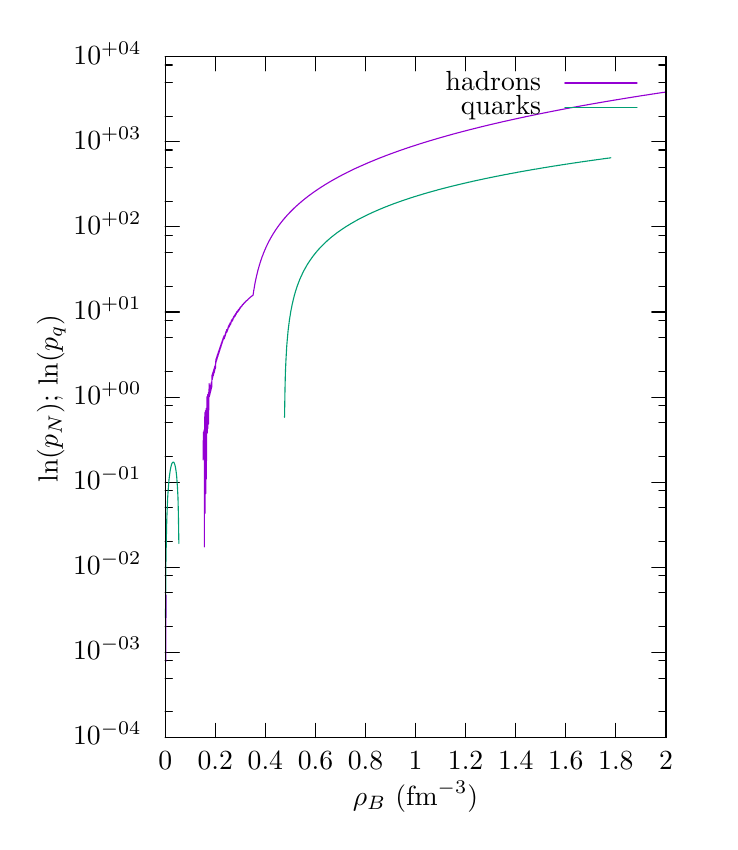
\begin{tikzpicture}[gnuplot]
%% generated with GNUPLOT 5.0p4 (Lua 5.2; terminal rev. 99, script rev. 100)
%% Thu Sep 29 16:33:17 2016
\path (0.000,0.000) rectangle (8.600,10.000);
\gpcolor{color=gp lt color border}
\gpsetlinetype{gp lt border}
\gpsetdashtype{gp dt solid}
\gpsetlinewidth{1.00}
\draw[gp path] (1.688,0.985)--(1.868,0.985);
\draw[gp path] (8.047,0.985)--(7.867,0.985);
\node[gp node right] at (1.504,0.985) {$10^{-04}$};
\draw[gp path] (1.688,1.310)--(1.778,1.310);
\draw[gp path] (8.047,1.310)--(7.957,1.310);
\draw[gp path] (1.688,1.740)--(1.778,1.740);
\draw[gp path] (8.047,1.740)--(7.957,1.740);
\draw[gp path] (1.688,1.961)--(1.778,1.961);
\draw[gp path] (8.047,1.961)--(7.957,1.961);
\draw[gp path] (1.688,2.066)--(1.868,2.066);
\draw[gp path] (8.047,2.066)--(7.867,2.066);
\node[gp node right] at (1.504,2.066) {$10^{-03}$};
\draw[gp path] (1.688,2.391)--(1.778,2.391);
\draw[gp path] (8.047,2.391)--(7.957,2.391);
\draw[gp path] (1.688,2.821)--(1.778,2.821);
\draw[gp path] (8.047,2.821)--(7.957,2.821);
\draw[gp path] (1.688,3.042)--(1.778,3.042);
\draw[gp path] (8.047,3.042)--(7.957,3.042);
\draw[gp path] (1.688,3.147)--(1.868,3.147);
\draw[gp path] (8.047,3.147)--(7.867,3.147);
\node[gp node right] at (1.504,3.147) {$10^{-02}$};
\draw[gp path] (1.688,3.472)--(1.778,3.472);
\draw[gp path] (8.047,3.472)--(7.957,3.472);
\draw[gp path] (1.688,3.902)--(1.778,3.902);
\draw[gp path] (8.047,3.902)--(7.957,3.902);
\draw[gp path] (1.688,4.123)--(1.778,4.123);
\draw[gp path] (8.047,4.123)--(7.957,4.123);
\draw[gp path] (1.688,4.227)--(1.868,4.227);
\draw[gp path] (8.047,4.227)--(7.867,4.227);
\node[gp node right] at (1.504,4.227) {$10^{-01}$};
\draw[gp path] (1.688,4.553)--(1.778,4.553);
\draw[gp path] (8.047,4.553)--(7.957,4.553);
\draw[gp path] (1.688,4.983)--(1.778,4.983);
\draw[gp path] (8.047,4.983)--(7.957,4.983);
\draw[gp path] (1.688,5.203)--(1.778,5.203);
\draw[gp path] (8.047,5.203)--(7.957,5.203);
\draw[gp path] (1.688,5.308)--(1.868,5.308);
\draw[gp path] (8.047,5.308)--(7.867,5.308);
\node[gp node right] at (1.504,5.308) {$10^{+00}$};
\draw[gp path] (1.688,5.633)--(1.778,5.633);
\draw[gp path] (8.047,5.633)--(7.957,5.633);
\draw[gp path] (1.688,6.063)--(1.778,6.063);
\draw[gp path] (8.047,6.063)--(7.957,6.063);
\draw[gp path] (1.688,6.284)--(1.778,6.284);
\draw[gp path] (8.047,6.284)--(7.957,6.284);
\draw[gp path] (1.688,6.389)--(1.868,6.389);
\draw[gp path] (8.047,6.389)--(7.867,6.389);
\node[gp node right] at (1.504,6.389) {$10^{+01}$};
\draw[gp path] (1.688,6.714)--(1.778,6.714);
\draw[gp path] (8.047,6.714)--(7.957,6.714);
\draw[gp path] (1.688,7.144)--(1.778,7.144);
\draw[gp path] (8.047,7.144)--(7.957,7.144);
\draw[gp path] (1.688,7.365)--(1.778,7.365);
\draw[gp path] (8.047,7.365)--(7.957,7.365);
\draw[gp path] (1.688,7.470)--(1.868,7.470);
\draw[gp path] (8.047,7.470)--(7.867,7.470);
\node[gp node right] at (1.504,7.470) {$10^{+02}$};
\draw[gp path] (1.688,7.795)--(1.778,7.795);
\draw[gp path] (8.047,7.795)--(7.957,7.795);
\draw[gp path] (1.688,8.225)--(1.778,8.225);
\draw[gp path] (8.047,8.225)--(7.957,8.225);
\draw[gp path] (1.688,8.446)--(1.778,8.446);
\draw[gp path] (8.047,8.446)--(7.957,8.446);
\draw[gp path] (1.688,8.550)--(1.868,8.550);
\draw[gp path] (8.047,8.550)--(7.867,8.550);
\node[gp node right] at (1.504,8.550) {$10^{+03}$};
\draw[gp path] (1.688,8.876)--(1.778,8.876);
\draw[gp path] (8.047,8.876)--(7.957,8.876);
\draw[gp path] (1.688,9.306)--(1.778,9.306);
\draw[gp path] (8.047,9.306)--(7.957,9.306);
\draw[gp path] (1.688,9.526)--(1.778,9.526);
\draw[gp path] (8.047,9.526)--(7.957,9.526);
\draw[gp path] (1.688,9.631)--(1.868,9.631);
\draw[gp path] (8.047,9.631)--(7.867,9.631);
\node[gp node right] at (1.504,9.631) {$10^{+04}$};
\draw[gp path] (1.688,0.985)--(1.688,1.165);
\draw[gp path] (1.688,9.631)--(1.688,9.451);
\node[gp node center] at (1.688,0.677) {$0$};
\draw[gp path] (2.324,0.985)--(2.324,1.165);
\draw[gp path] (2.324,9.631)--(2.324,9.451);
\node[gp node center] at (2.324,0.677) {$0.2$};
\draw[gp path] (2.960,0.985)--(2.960,1.165);
\draw[gp path] (2.960,9.631)--(2.960,9.451);
\node[gp node center] at (2.960,0.677) {$0.4$};
\draw[gp path] (3.596,0.985)--(3.596,1.165);
\draw[gp path] (3.596,9.631)--(3.596,9.451);
\node[gp node center] at (3.596,0.677) {$0.6$};
\draw[gp path] (4.232,0.985)--(4.232,1.165);
\draw[gp path] (4.232,9.631)--(4.232,9.451);
\node[gp node center] at (4.232,0.677) {$0.8$};
\draw[gp path] (4.868,0.985)--(4.868,1.165);
\draw[gp path] (4.868,9.631)--(4.868,9.451);
\node[gp node center] at (4.868,0.677) {$1$};
\draw[gp path] (5.503,0.985)--(5.503,1.165);
\draw[gp path] (5.503,9.631)--(5.503,9.451);
\node[gp node center] at (5.503,0.677) {$1.2$};
\draw[gp path] (6.139,0.985)--(6.139,1.165);
\draw[gp path] (6.139,9.631)--(6.139,9.451);
\node[gp node center] at (6.139,0.677) {$1.4$};
\draw[gp path] (6.775,0.985)--(6.775,1.165);
\draw[gp path] (6.775,9.631)--(6.775,9.451);
\node[gp node center] at (6.775,0.677) {$1.6$};
\draw[gp path] (7.411,0.985)--(7.411,1.165);
\draw[gp path] (7.411,9.631)--(7.411,9.451);
\node[gp node center] at (7.411,0.677) {$1.8$};
\draw[gp path] (8.047,0.985)--(8.047,1.165);
\draw[gp path] (8.047,9.631)--(8.047,9.451);
\node[gp node center] at (8.047,0.677) {$2$};
\draw[gp path] (1.688,9.631)--(1.688,0.985)--(8.047,0.985)--(8.047,9.631)--cycle;
\node[gp node center,rotate=-270] at (0.246,5.308) {$\ln(p_N)$; $\ln(p_q)$};
\node[gp node center] at (4.867,0.215) {$\rho_B$ ($\rm{fm}^{-3}$)};
\node[gp node right] at (6.579,9.297) {hadrons};
\gpcolor{rgb color={0.580,0.000,0.827}}
\draw[gp path] (6.763,9.297)--(7.679,9.297);
\draw[gp path] (1.695,1.949)--(1.698,2.796);
\draw[gp path] (2.170,4.510)--(2.172,4.863);
\draw[gp path] (2.179,4.561)--(2.181,4.893);
\draw[gp path] (2.185,3.406)--(2.187,4.616)--(2.189,4.925)--(2.191,5.111)--(2.193,3.832)%
  --(2.196,4.673)--(2.198,4.959)--(2.200,5.137)--(2.202,4.083)--(2.204,4.732)--(2.206,4.996)%
  --(2.208,5.165)--(2.210,4.268)--(2.213,4.792)--(2.215,5.034)--(2.217,5.195)--(2.219,5.315)%
  --(2.221,4.851)--(2.223,5.074)--(2.225,5.225)--(2.227,5.340)--(2.229,4.909)--(2.232,5.114)%
  --(2.234,5.257)--(2.236,5.367)--(2.238,4.967)--(2.240,5.155)--(2.242,5.289)--(2.244,5.394)%
  --(2.246,5.481)--(2.249,5.314)--(2.251,5.415)--(2.253,5.331)--(2.255,5.430)--(2.257,5.347)%
  --(2.259,5.444)--(2.261,5.364)--(2.263,5.458)--(2.266,5.381)--(2.268,5.473)--(2.270,5.398)%
  --(2.272,5.488)--(2.274,5.415)--(2.276,5.502)--(2.278,5.432)--(2.280,5.517)--(2.282,5.589)%
  --(2.285,5.532)--(2.287,5.603)--(2.289,5.547)--(2.291,5.616)--(2.293,5.562)--(2.295,5.629)%
  --(2.297,5.577)--(2.299,5.643)--(2.302,5.591)--(2.304,5.656)--(2.306,5.606)--(2.308,5.670)%
  --(2.310,5.621)--(2.312,5.683)--(2.314,5.636)--(2.316,5.697)--(2.318,5.651)--(2.321,5.710)%
  --(2.323,5.666)--(2.325,5.724)--(2.327,5.681)--(2.329,5.738)--(2.331,5.788)--(2.333,5.751)%
  --(2.335,5.801)--(2.338,5.765)--(2.340,5.814)--(2.342,5.778)--(2.344,5.826)--(2.346,5.792)%
  --(2.348,5.839)--(2.350,5.805)--(2.352,5.851)--(2.355,5.819)--(2.357,5.864)--(2.359,5.832)%
  --(2.361,5.876)--(2.363,5.846)--(2.365,5.889)--(2.367,5.859)--(2.369,5.901)--(2.371,5.872)%
  --(2.374,5.914)--(2.376,5.886)--(2.378,5.926)--(2.380,5.899)--(2.382,5.939)--(2.384,5.912)%
  --(2.386,5.951)--(2.388,5.925)--(2.391,5.964)--(2.393,5.939)--(2.395,5.976)--(2.397,5.952)%
  --(2.399,5.988)--(2.401,5.965)--(2.403,6.001)--(2.405,5.978)--(2.408,6.013)--(2.410,5.991)%
  --(2.412,6.025)--(2.414,6.004)--(2.416,6.037)--(2.418,6.016)--(2.420,6.050)--(2.422,6.029)%
  --(2.424,6.062)--(2.427,6.042)--(2.429,6.074)--(2.431,6.054)--(2.433,6.086)--(2.435,6.067)%
  --(2.437,6.048)--(2.439,6.080)--(2.441,6.061)--(2.444,6.092)--(2.446,6.074)--(2.448,6.104)%
  --(2.450,6.087)--(2.452,6.117)--(2.454,6.100)--(2.456,6.129)--(2.458,6.112)--(2.460,6.141)%
  --(2.463,6.125)--(2.465,6.153)--(2.467,6.138)--(2.469,6.166)--(2.471,6.150)--(2.473,6.135)%
  --(2.475,6.163)--(2.477,6.148)--(2.480,6.175)--(2.482,6.161)--(2.484,6.188)--(2.486,6.174)%
  --(2.488,6.200)--(2.490,6.186)--(2.492,6.212)--(2.494,6.199)--(2.497,6.224)--(2.499,6.212)%
  --(2.501,6.199)--(2.503,6.224)--(2.505,6.212)--(2.507,6.236)--(2.509,6.224)--(2.511,6.249)%
  --(2.513,6.237)--(2.516,6.225)--(2.518,6.250)--(2.520,6.238)--(2.522,6.262)--(2.524,6.251)%
  --(2.526,6.275)--(2.528,6.264)--(2.530,6.287)--(2.533,6.277)--(2.535,6.266)--(2.537,6.289)%
  --(2.539,6.279)--(2.541,6.302)--(2.543,6.292)--(2.545,6.282)--(2.547,6.305)--(2.550,6.296)%
  --(2.552,6.318)--(2.554,6.309)--(2.556,6.330)--(2.558,6.322)--(2.560,6.313)--(2.562,6.335)%
  --(2.564,6.326)--(2.566,6.347)--(2.569,6.339)--(2.571,6.331)--(2.573,6.352)--(2.575,6.344)%
  --(2.577,6.337)--(2.579,6.358)--(2.581,6.350)--(2.583,6.371)--(2.586,6.363)--(2.588,6.356)%
  --(2.590,6.377)--(2.592,6.370)--(2.594,6.390)--(2.596,6.383)--(2.598,6.377)--(2.600,6.397)%
  --(2.602,6.390)--(2.605,6.384)--(2.607,6.404)--(2.609,6.398)--(2.611,6.392)--(2.613,6.412)%
  --(2.615,6.406)--(2.617,6.401)--(2.619,6.420)--(2.622,6.415)--(2.624,6.410)--(2.626,6.429)%
  --(2.628,6.424)--(2.630,6.419)--(2.632,6.438)--(2.634,6.434)--(2.636,6.429)--(2.639,6.448)%
  --(2.641,6.438)--(2.643,6.445)--(2.645,6.452)--(2.647,6.449)--(2.649,6.456)--(2.651,6.452)%
  --(2.653,6.460)--(2.655,6.456)--(2.658,6.464)--(2.660,6.461)--(2.662,6.468)--(2.664,6.476)%
  --(2.666,6.473)--(2.668,6.481)--(2.670,6.478)--(2.672,6.486)--(2.675,6.484)--(2.677,6.482)%
  --(2.679,6.489)--(2.681,6.488)--(2.683,6.496)--(2.685,6.494)--(2.687,6.502)--(2.689,6.501)%
  --(2.691,6.500)--(2.694,6.508)--(2.696,6.507)--(2.698,6.506)--(2.700,6.514)--(2.702,6.514)%
  --(2.704,6.514)--(2.706,6.522)--(2.708,6.522)--(2.711,6.522)--(2.713,6.522)--(2.715,6.531)%
  --(2.717,6.532)--(2.719,6.532)--(2.721,6.533)--(2.723,6.534)--(2.725,6.536)--(2.728,6.537)%
  --(2.730,6.539)--(2.732,6.541)--(2.734,6.543)--(2.736,6.545)--(2.738,6.547)--(2.740,6.550)%
  --(2.742,6.552)--(2.744,6.555)--(2.747,6.558)--(2.749,6.561)--(2.751,6.559)--(2.753,6.562)%
  --(2.755,6.566)--(2.757,6.565)--(2.759,6.569)--(2.761,6.569)--(2.764,6.571)--(2.766,6.574)%
  --(2.768,6.577)--(2.770,6.577)--(2.772,6.578)--(2.774,6.580)--(2.776,6.582)--(2.778,6.584)%
  --(2.781,6.585)--(2.783,6.588)--(2.785,6.588)--(2.787,6.591)--(2.789,6.591)--(2.791,6.594)%
  --(2.793,6.595)--(2.795,6.597)--(2.797,6.598)--(2.800,6.600)--(2.802,6.601)--(2.804,6.605)%
  --(2.806,6.620)--(2.808,6.634)--(2.810,6.648)--(2.812,6.662)--(2.814,6.675)--(2.817,6.688)%
  --(2.819,6.700)--(2.821,6.712)--(2.823,6.724)--(2.825,6.736)--(2.827,6.747)--(2.829,6.759)%
  --(2.831,6.769)--(2.833,6.780)--(2.836,6.791)--(2.838,6.801)--(2.840,6.811)--(2.842,6.821)%
  --(2.844,6.830)--(2.846,6.840)--(2.848,6.849)--(2.850,6.858)--(2.853,6.867)--(2.855,6.876)%
  --(2.857,6.885)--(2.859,6.893)--(2.861,6.902)--(2.863,6.910)--(2.865,6.918)--(2.867,6.926)%
  --(2.870,6.934)--(2.872,6.942)--(2.874,6.949)--(2.876,6.957)--(2.878,6.964)--(2.880,6.971)%
  --(2.882,6.979)--(2.884,6.986)--(2.886,6.993)--(2.889,7.000)--(2.891,7.007)--(2.893,7.013)%
  --(2.895,7.020)--(2.897,7.027)--(2.899,7.033)--(2.901,7.040)--(2.903,7.046)--(2.906,7.052)%
  --(2.908,7.058)--(2.910,7.065)--(2.912,7.071)--(2.914,7.077)--(2.916,7.083)--(2.918,7.088)%
  --(2.920,7.094)--(2.923,7.100)--(2.925,7.106)--(2.927,7.111)--(2.929,7.117)--(2.931,7.122)%
  --(2.933,7.128)--(2.935,7.133)--(2.937,7.139)--(2.939,7.144)--(2.942,7.149)--(2.944,7.154)%
  --(2.946,7.159)--(2.948,7.164)--(2.950,7.170)--(2.952,7.175)--(2.954,7.179)--(2.956,7.184)%
  --(2.959,7.189)--(2.961,7.194)--(2.963,7.199)--(2.965,7.204)--(2.967,7.208)--(2.969,7.213)%
  --(2.971,7.218)--(2.973,7.222)--(2.975,7.227)--(2.978,7.231)--(2.980,7.236)--(2.982,7.240)%
  --(2.984,7.245)--(2.986,7.249)--(2.988,7.253)--(2.990,7.258)--(2.992,7.262)--(2.995,7.266)%
  --(2.997,7.270)--(2.999,7.274)--(3.001,7.279)--(3.003,7.283)--(3.005,7.287)--(3.007,7.291)%
  --(3.009,7.295)--(3.012,7.299)--(3.014,7.303)--(3.016,7.307)--(3.018,7.311)--(3.020,7.315)%
  --(3.022,7.318)--(3.024,7.322)--(3.026,7.326)--(3.028,7.330)--(3.031,7.334)--(3.033,7.337)%
  --(3.035,7.341)--(3.037,7.345)--(3.039,7.348)--(3.041,7.352)--(3.043,7.356)--(3.045,7.359)%
  --(3.048,7.363)--(3.050,7.366)--(3.052,7.370)--(3.054,7.373)--(3.056,7.377)--(3.058,7.380)%
  --(3.060,7.384)--(3.062,7.387)--(3.064,7.391)--(3.067,7.394)--(3.069,7.397)--(3.071,7.401)%
  --(3.073,7.404)--(3.075,7.407)--(3.077,7.411)--(3.079,7.414)--(3.081,7.417)--(3.084,7.420)%
  --(3.086,7.424)--(3.088,7.427)--(3.090,7.430)--(3.092,7.433)--(3.094,7.436)--(3.096,7.439)%
  --(3.098,7.442)--(3.101,7.446)--(3.103,7.449)--(3.105,7.452)--(3.107,7.455)--(3.109,7.458)%
  --(3.111,7.461)--(3.113,7.464)--(3.115,7.467)--(3.117,7.470)--(3.120,7.473)--(3.122,7.476)%
  --(3.124,7.479)--(3.126,7.482)--(3.128,7.484)--(3.130,7.487)--(3.132,7.490)--(3.134,7.493)%
  --(3.137,7.496)--(3.139,7.499)--(3.141,7.502)--(3.143,7.504)--(3.145,7.507)--(3.147,7.510)%
  --(3.149,7.513)--(3.151,7.515)--(3.154,7.518)--(3.156,7.521)--(3.158,7.524)--(3.160,7.526)%
  --(3.162,7.529)--(3.164,7.532)--(3.166,7.534)--(3.168,7.537)--(3.170,7.540)--(3.173,7.542)%
  --(3.175,7.545)--(3.177,7.548)--(3.179,7.550)--(3.181,7.553)--(3.183,7.555)--(3.185,7.558)%
  --(3.187,7.561)--(3.190,7.563)--(3.192,7.566)--(3.194,7.568)--(3.196,7.571)--(3.198,7.573)%
  --(3.200,7.576)--(3.202,7.578)--(3.204,7.581)--(3.206,7.583)--(3.209,7.586)--(3.211,7.588)%
  --(3.213,7.590)--(3.215,7.593)--(3.217,7.595)--(3.219,7.598)--(3.221,7.600)--(3.223,7.602)%
  --(3.226,7.605)--(3.228,7.607)--(3.230,7.610)--(3.232,7.612)--(3.234,7.614)--(3.236,7.617)%
  --(3.238,7.619)--(3.240,7.621)--(3.243,7.624)--(3.245,7.626)--(3.247,7.628)--(3.249,7.630)%
  --(3.251,7.633)--(3.253,7.635)--(3.255,7.637)--(3.257,7.640)--(3.259,7.642)--(3.262,7.644)%
  --(3.264,7.646)--(3.266,7.648)--(3.268,7.651)--(3.270,7.653)--(3.272,7.655)--(3.274,7.657)%
  --(3.276,7.659)--(3.279,7.662)--(3.281,7.664)--(3.283,7.666)--(3.285,7.668)--(3.287,7.670)%
  --(3.289,7.672)--(3.291,7.675)--(3.293,7.677)--(3.295,7.679)--(3.298,7.681)--(3.300,7.683)%
  --(3.302,7.685)--(3.304,7.687)--(3.306,7.689)--(3.308,7.691)--(3.310,7.693)--(3.312,7.696)%
  --(3.315,7.698)--(3.317,7.700)--(3.319,7.702)--(3.321,7.704)--(3.323,7.706)--(3.325,7.708)%
  --(3.327,7.710)--(3.329,7.712)--(3.332,7.714)--(3.334,7.716)--(3.336,7.718)--(3.338,7.720)%
  --(3.340,7.722)--(3.342,7.724)--(3.344,7.726)--(3.346,7.728)--(3.348,7.730)--(3.351,7.732)%
  --(3.353,7.734)--(3.355,7.736)--(3.357,7.737)--(3.359,7.739)--(3.361,7.741)--(3.363,7.743)%
  --(3.365,7.745)--(3.368,7.747)--(3.370,7.749)--(3.372,7.751)--(3.374,7.753)--(3.376,7.755)%
  --(3.378,7.756)--(3.380,7.758)--(3.382,7.760)--(3.385,7.762)--(3.387,7.764)--(3.389,7.766)%
  --(3.391,7.768)--(3.393,7.770)--(3.395,7.771)--(3.397,7.773)--(3.399,7.775)--(3.401,7.777)%
  --(3.404,7.779)--(3.406,7.780)--(3.408,7.782)--(3.410,7.784)--(3.412,7.786)--(3.414,7.788)%
  --(3.416,7.789)--(3.418,7.791)--(3.421,7.793)--(3.423,7.795)--(3.425,7.797)--(3.427,7.798)%
  --(3.429,7.800)--(3.431,7.802)--(3.433,7.804)--(3.435,7.805)--(3.437,7.807)--(3.440,7.809)%
  --(3.442,7.811)--(3.444,7.812)--(3.446,7.814)--(3.448,7.816)--(3.450,7.817)--(3.452,7.819)%
  --(3.454,7.821)--(3.457,7.823)--(3.459,7.824)--(3.461,7.826)--(3.463,7.828)--(3.465,7.829)%
  --(3.467,7.831)--(3.469,7.833)--(3.471,7.834)--(3.474,7.836)--(3.476,7.838)--(3.478,7.839)%
  --(3.480,7.841)--(3.482,7.843)--(3.484,7.844)--(3.486,7.846)--(3.488,7.848)--(3.490,7.849)%
  --(3.493,7.851)--(3.495,7.853)--(3.497,7.854)--(3.499,7.856)--(3.501,7.857)--(3.503,7.859)%
  --(3.505,7.861)--(3.507,7.862)--(3.510,7.864)--(3.512,7.865)--(3.514,7.867)--(3.516,7.869)%
  --(3.518,7.870)--(3.520,7.872)--(3.522,7.873)--(3.524,7.875)--(3.527,7.877)--(3.529,7.878)%
  --(3.531,7.880)--(3.533,7.881)--(3.535,7.883)--(3.537,7.884)--(3.539,7.886)--(3.541,7.887)%
  --(3.543,7.889)--(3.546,7.891)--(3.548,7.892)--(3.550,7.894)--(3.552,7.895)--(3.554,7.897)%
  --(3.556,7.898)--(3.558,7.900)--(3.560,7.901)--(3.563,7.903)--(3.565,7.904)--(3.567,7.906)%
  --(3.569,7.907)--(3.571,7.909)--(3.573,7.910)--(3.575,7.912)--(3.577,7.913)--(3.579,7.915)%
  --(3.582,7.916)--(3.584,7.918)--(3.586,7.919)--(3.588,7.921)--(3.590,7.922)--(3.592,7.924)%
  --(3.594,7.925)--(3.596,7.927)--(3.599,7.928)--(3.601,7.929)--(3.603,7.931)--(3.605,7.932)%
  --(3.607,7.934)--(3.609,7.935)--(3.611,7.937)--(3.613,7.938)--(3.616,7.940)--(3.618,7.941)%
  --(3.620,7.942)--(3.622,7.944)--(3.624,7.945)--(3.626,7.947)--(3.628,7.948)--(3.630,7.950)%
  --(3.632,7.951)--(3.635,7.952)--(3.637,7.954)--(3.639,7.955)--(3.641,7.957)--(3.643,7.958)%
  --(3.645,7.959)--(3.647,7.961)--(3.649,7.962)--(3.652,7.964)--(3.654,7.965)--(3.656,7.966)%
  --(3.658,7.968)--(3.660,7.969)--(3.662,7.970)--(3.664,7.972)--(3.666,7.973)--(3.668,7.975)%
  --(3.671,7.976)--(3.673,7.977)--(3.675,7.979)--(3.677,7.980)--(3.679,7.981)--(3.681,7.983)%
  --(3.683,7.984)--(3.685,7.985)--(3.688,7.987)--(3.690,7.988)--(3.692,7.989)--(3.694,7.991)%
  --(3.696,7.992)--(3.698,7.993)--(3.700,7.995)--(3.702,7.996)--(3.705,7.997)--(3.707,7.999)%
  --(3.709,8.000)--(3.711,8.001)--(3.713,8.003)--(3.715,8.004)--(3.717,8.005)--(3.719,8.007)%
  --(3.721,8.008)--(3.724,8.009)--(3.726,8.011)--(3.728,8.012)--(3.730,8.013)--(3.732,8.014)%
  --(3.734,8.016)--(3.736,8.017)--(3.738,8.018)--(3.741,8.020)--(3.743,8.021)--(3.745,8.022)%
  --(3.747,8.023)--(3.749,8.025)--(3.751,8.026)--(3.753,8.027)--(3.755,8.029)--(3.758,8.030)%
  --(3.760,8.031)--(3.762,8.032)--(3.764,8.034)--(3.766,8.035)--(3.768,8.036)--(3.770,8.037)%
  --(3.772,8.039)--(3.774,8.040)--(3.777,8.041)--(3.779,8.042)--(3.781,8.044)--(3.783,8.045)%
  --(3.785,8.046)--(3.787,8.047)--(3.789,8.049)--(3.791,8.050)--(3.794,8.051)--(3.796,8.052)%
  --(3.798,8.053)--(3.800,8.055)--(3.802,8.056)--(3.804,8.057)--(3.806,8.058)--(3.808,8.060)%
  --(3.810,8.061)--(3.813,8.062)--(3.815,8.063)--(3.817,8.064)--(3.819,8.066)--(3.821,8.067)%
  --(3.823,8.068)--(3.825,8.069)--(3.827,8.070)--(3.830,8.072)--(3.832,8.073)--(3.834,8.074)%
  --(3.836,8.075)--(3.838,8.076)--(3.840,8.078)--(3.842,8.079)--(3.844,8.080)--(3.847,8.081)%
  --(3.849,8.082)--(3.851,8.083)--(3.853,8.085)--(3.855,8.086)--(3.857,8.087)--(3.859,8.088)%
  --(3.861,8.089)--(3.863,8.090)--(3.866,8.092)--(3.868,8.093)--(3.870,8.094)--(3.872,8.095)%
  --(3.874,8.096)--(3.876,8.097)--(3.878,8.099)--(3.880,8.100)--(3.883,8.101)--(3.885,8.102)%
  --(3.887,8.103)--(3.889,8.104)--(3.891,8.105)--(3.893,8.107)--(3.895,8.108)--(3.897,8.109)%
  --(3.900,8.110)--(3.902,8.111)--(3.904,8.112)--(3.906,8.113)--(3.908,8.115)--(3.910,8.116)%
  --(3.912,8.117)--(3.914,8.118)--(3.916,8.119)--(3.919,8.120)--(3.921,8.121)--(3.923,8.122)%
  --(3.925,8.124)--(3.927,8.125)--(3.929,8.126)--(3.931,8.127)--(3.933,8.128)--(3.936,8.129)%
  --(3.938,8.130)--(3.940,8.131)--(3.942,8.132)--(3.944,8.133)--(3.946,8.135)--(3.948,8.136)%
  --(3.950,8.137)--(3.952,8.138)--(3.955,8.139)--(3.957,8.140)--(3.959,8.141)--(3.961,8.142)%
  --(3.963,8.143)--(3.965,8.144)--(3.967,8.145)--(3.969,8.147)--(3.972,8.148)--(3.974,8.149)%
  --(3.976,8.150)--(3.978,8.151)--(3.980,8.152)--(3.982,8.153)--(3.984,8.154)--(3.986,8.155)%
  --(3.989,8.156)--(3.991,8.157)--(3.993,8.158)--(3.995,8.159)--(3.997,8.160)--(3.999,8.162)%
  --(4.001,8.163)--(4.003,8.164)--(4.005,8.165)--(4.008,8.166)--(4.010,8.167)--(4.012,8.168)%
  --(4.014,8.169)--(4.016,8.170)--(4.018,8.171)--(4.020,8.172)--(4.022,8.173)--(4.025,8.174)%
  --(4.027,8.175)--(4.029,8.176)--(4.031,8.177)--(4.033,8.178)--(4.035,8.179)--(4.037,8.180)%
  --(4.039,8.181)--(4.041,8.182)--(4.044,8.183)--(4.046,8.184)--(4.048,8.186)--(4.050,8.187)%
  --(4.052,8.188)--(4.054,8.189)--(4.056,8.190)--(4.058,8.191)--(4.061,8.192)--(4.063,8.193)%
  --(4.065,8.194)--(4.067,8.195)--(4.069,8.196)--(4.071,8.197)--(4.073,8.198)--(4.075,8.199)%
  --(4.078,8.200)--(4.080,8.201)--(4.082,8.202)--(4.084,8.203)--(4.086,8.204)--(4.088,8.205)%
  --(4.090,8.206)--(4.092,8.207)--(4.094,8.208)--(4.097,8.209)--(4.099,8.210)--(4.101,8.211)%
  --(4.103,8.212)--(4.105,8.213)--(4.107,8.214)--(4.109,8.215)--(4.111,8.216)--(4.114,8.217)%
  --(4.116,8.218)--(4.118,8.219)--(4.120,8.220)--(4.122,8.221)--(4.124,8.222)--(4.126,8.223)%
  --(4.128,8.224)--(4.131,8.225)--(4.133,8.225)--(4.135,8.226)--(4.137,8.227)--(4.139,8.228)%
  --(4.141,8.229)--(4.143,8.230)--(4.145,8.231)--(4.147,8.232)--(4.150,8.233)--(4.152,8.234)%
  --(4.154,8.235)--(4.156,8.236)--(4.158,8.237)--(4.160,8.238)--(4.162,8.239)--(4.164,8.240)%
  --(4.167,8.241)--(4.169,8.242)--(4.171,8.243)--(4.173,8.244)--(4.175,8.245)--(4.177,8.246)%
  --(4.179,8.247)--(4.181,8.248)--(4.183,8.249)--(4.186,8.249)--(4.188,8.250)--(4.190,8.251)%
  --(4.192,8.252)--(4.194,8.253)--(4.196,8.254)--(4.198,8.255)--(4.200,8.256)--(4.203,8.257)%
  --(4.205,8.258)--(4.207,8.259)--(4.209,8.260)--(4.211,8.261)--(4.213,8.262)--(4.215,8.263)%
  --(4.217,8.264)--(4.220,8.264)--(4.222,8.265)--(4.224,8.266)--(4.226,8.267)--(4.228,8.268)%
  --(4.230,8.269)--(4.232,8.270)--(4.234,8.271)--(4.236,8.272)--(4.239,8.273)--(4.241,8.274)%
  --(4.243,8.275)--(4.245,8.275)--(4.247,8.276)--(4.249,8.277)--(4.251,8.278)--(4.253,8.279)%
  --(4.256,8.280)--(4.258,8.281)--(4.260,8.282)--(4.262,8.283)--(4.264,8.284)--(4.266,8.285)%
  --(4.268,8.285)--(4.270,8.286)--(4.273,8.287)--(4.275,8.288)--(4.277,8.289)--(4.279,8.290)%
  --(4.281,8.291)--(4.283,8.292)--(4.285,8.293)--(4.287,8.294)--(4.289,8.294)--(4.292,8.295)%
  --(4.294,8.296)--(4.296,8.297)--(4.298,8.298)--(4.300,8.299)--(4.302,8.300)--(4.304,8.301)%
  --(4.306,8.302)--(4.309,8.302)--(4.311,8.303)--(4.313,8.304)--(4.315,8.305)--(4.317,8.306)%
  --(4.319,8.307)--(4.321,8.308)--(4.323,8.309)--(4.325,8.309)--(4.328,8.310)--(4.330,8.311)%
  --(4.332,8.312)--(4.334,8.313)--(4.336,8.314)--(4.338,8.315)--(4.340,8.316)--(4.342,8.316)%
  --(4.345,8.317)--(4.347,8.318)--(4.349,8.319)--(4.351,8.320)--(4.353,8.321)--(4.355,8.322)%
  --(4.357,8.322)--(4.359,8.323)--(4.362,8.324)--(4.364,8.325)--(4.366,8.326)--(4.368,8.327)%
  --(4.370,8.328)--(4.372,8.328)--(4.374,8.329)--(4.376,8.330)--(4.378,8.331)--(4.381,8.332)%
  --(4.383,8.333)--(4.385,8.334)--(4.387,8.334)--(4.389,8.335)--(4.391,8.336)--(4.393,8.337)%
  --(4.395,8.338)--(4.398,8.339)--(4.400,8.339)--(4.402,8.340)--(4.404,8.341)--(4.406,8.342)%
  --(4.408,8.343)--(4.410,8.344)--(4.412,8.345)--(4.414,8.345)--(4.417,8.346)--(4.419,8.347)%
  --(4.421,8.348)--(4.423,8.349)--(4.425,8.350)--(4.427,8.350)--(4.429,8.351)--(4.431,8.352)%
  --(4.434,8.353)--(4.436,8.354)--(4.438,8.355)--(4.440,8.355)--(4.442,8.356)--(4.444,8.357)%
  --(4.446,8.358)--(4.448,8.359)--(4.451,8.359)--(4.453,8.360)--(4.455,8.361)--(4.457,8.362)%
  --(4.459,8.363)--(4.461,8.364)--(4.463,8.364)--(4.465,8.365)--(4.467,8.366)--(4.470,8.367)%
  --(4.472,8.368)--(4.474,8.368)--(4.476,8.369)--(4.478,8.370)--(4.480,8.371)--(4.482,8.372)%
  --(4.484,8.372)--(4.487,8.373)--(4.489,8.374)--(4.491,8.375)--(4.493,8.376)--(4.495,8.377)%
  --(4.497,8.377)--(4.499,8.378)--(4.501,8.379)--(4.504,8.380)--(4.506,8.381)--(4.508,8.381)%
  --(4.510,8.382)--(4.512,8.383)--(4.514,8.384)--(4.516,8.385)--(4.518,8.385)--(4.520,8.386)%
  --(4.523,8.387)--(4.525,8.388)--(4.527,8.388)--(4.529,8.389)--(4.531,8.390)--(4.533,8.391)%
  --(4.535,8.392)--(4.537,8.392)--(4.540,8.393)--(4.542,8.394)--(4.544,8.395)--(4.546,8.396)%
  --(4.548,8.396)--(4.550,8.397)--(4.552,8.398)--(4.554,8.399)--(4.556,8.400)--(4.559,8.400)%
  --(4.561,8.401)--(4.563,8.402)--(4.565,8.403)--(4.567,8.403)--(4.569,8.404)--(4.571,8.405)%
  --(4.573,8.406)--(4.576,8.407)--(4.578,8.407)--(4.580,8.408)--(4.582,8.409)--(4.584,8.410)%
  --(4.586,8.410)--(4.588,8.411)--(4.590,8.412)--(4.593,8.413)--(4.595,8.413)--(4.597,8.414)%
  --(4.599,8.415)--(4.601,8.416)--(4.603,8.417)--(4.605,8.417)--(4.607,8.418)--(4.609,8.419)%
  --(4.612,8.420)--(4.614,8.420)--(4.616,8.421)--(4.618,8.422)--(4.620,8.423)--(4.622,8.423)%
  --(4.624,8.424)--(4.626,8.425)--(4.629,8.426)--(4.631,8.426)--(4.633,8.427)--(4.635,8.428)%
  --(4.637,8.429)--(4.639,8.429)--(4.641,8.430)--(4.643,8.431)--(4.646,8.432)--(4.648,8.432)%
  --(4.650,8.433)--(4.652,8.434)--(4.654,8.435)--(4.656,8.435)--(4.658,8.436)--(4.660,8.437)%
  --(4.662,8.438)--(4.665,8.438)--(4.667,8.439)--(4.669,8.440)--(4.671,8.441)--(4.673,8.441)%
  --(4.675,8.442)--(4.677,8.443)--(4.679,8.444)--(4.682,8.444)--(4.684,8.445)--(4.686,8.446)%
  --(4.688,8.447)--(4.690,8.447)--(4.692,8.448)--(4.694,8.449)--(4.696,8.450)--(4.698,8.450)%
  --(4.701,8.451)--(4.703,8.452)--(4.705,8.452)--(4.707,8.453)--(4.709,8.454)--(4.711,8.455)%
  --(4.713,8.455)--(4.715,8.456)--(4.718,8.457)--(4.720,8.458)--(4.722,8.458)--(4.724,8.459)%
  --(4.726,8.460)--(4.728,8.460)--(4.730,8.461)--(4.732,8.462)--(4.735,8.463)--(4.737,8.463)%
  --(4.739,8.464)--(4.741,8.465)--(4.743,8.466)--(4.745,8.466)--(4.747,8.467)--(4.749,8.468)%
  --(4.751,8.468)--(4.754,8.469)--(4.756,8.470)--(4.758,8.471)--(4.760,8.471)--(4.762,8.472)%
  --(4.764,8.473)--(4.766,8.473)--(4.768,8.474)--(4.771,8.475)--(4.773,8.476)--(4.775,8.476)%
  --(4.777,8.477)--(4.779,8.478)--(4.781,8.478)--(4.783,8.479)--(4.785,8.480)--(4.787,8.481)%
  --(4.790,8.481)--(4.792,8.482)--(4.794,8.483)--(4.796,8.483)--(4.798,8.484)--(4.800,8.485)%
  --(4.802,8.485)--(4.804,8.486)--(4.807,8.487)--(4.809,8.488)--(4.811,8.488)--(4.813,8.489)%
  --(4.815,8.490)--(4.817,8.490)--(4.819,8.491)--(4.821,8.492)--(4.824,8.492)--(4.826,8.493)%
  --(4.828,8.494)--(4.830,8.495)--(4.832,8.495)--(4.834,8.496)--(4.836,8.497)--(4.838,8.497)%
  --(4.840,8.498)--(4.843,8.499)--(4.845,8.499)--(4.847,8.500)--(4.849,8.501)--(4.851,8.501)%
  --(4.853,8.502)--(4.855,8.503)--(4.857,8.504)--(4.860,8.504)--(4.862,8.505)--(4.864,8.506)%
  --(4.866,8.506)--(4.868,8.507)--(4.870,8.508)--(4.872,8.508)--(4.874,8.509)--(4.877,8.510)%
  --(4.879,8.510)--(4.881,8.511)--(4.883,8.512)--(4.885,8.512)--(4.887,8.513)--(4.889,8.514)%
  --(4.891,8.514)--(4.893,8.515)--(4.896,8.516)--(4.898,8.516)--(4.900,8.517)--(4.902,8.518)%
  --(4.904,8.519)--(4.906,8.519)--(4.908,8.520)--(4.910,8.521)--(4.913,8.521)--(4.915,8.522)%
  --(4.917,8.523)--(4.919,8.523)--(4.921,8.524)--(4.923,8.525)--(4.925,8.525)--(4.927,8.526)%
  --(4.929,8.527)--(4.932,8.527)--(4.934,8.528)--(4.936,8.529)--(4.938,8.529)--(4.940,8.530)%
  --(4.942,8.531)--(4.944,8.531)--(4.946,8.532)--(4.949,8.533)--(4.951,8.533)--(4.953,8.534)%
  --(4.955,8.535)--(4.957,8.535)--(4.959,8.536)--(4.961,8.537)--(4.963,8.537)--(4.966,8.538)%
  --(4.968,8.539)--(4.970,8.539)--(4.972,8.540)--(4.974,8.541)--(4.976,8.541)--(4.978,8.542)%
  --(4.980,8.543)--(4.982,8.543)--(4.985,8.544)--(4.987,8.544)--(4.989,8.545)--(4.991,8.546)%
  --(4.993,8.546)--(4.995,8.547)--(4.997,8.548)--(4.999,8.548)--(5.002,8.549)--(5.004,8.550)%
  --(5.006,8.550)--(5.008,8.551)--(5.010,8.552)--(5.012,8.552)--(5.014,8.553)--(5.016,8.554)%
  --(5.019,8.554)--(5.021,8.555)--(5.023,8.556)--(5.025,8.556)--(5.027,8.557)--(5.029,8.557)%
  --(5.031,8.558)--(5.033,8.559)--(5.035,8.559)--(5.038,8.560)--(5.040,8.561)--(5.042,8.561)%
  --(5.044,8.562)--(5.046,8.563)--(5.048,8.563)--(5.050,8.564)--(5.052,8.565)--(5.055,8.565)%
  --(5.057,8.566)--(5.059,8.566)--(5.061,8.567)--(5.063,8.568)--(5.065,8.568)--(5.067,8.569)%
  --(5.069,8.570)--(5.071,8.570)--(5.074,8.571)--(5.076,8.572)--(5.078,8.572)--(5.080,8.573)%
  --(5.082,8.573)--(5.084,8.574)--(5.086,8.575)--(5.088,8.575)--(5.091,8.576)--(5.093,8.577)%
  --(5.095,8.577)--(5.097,8.578)--(5.099,8.578)--(5.101,8.579)--(5.103,8.580)--(5.105,8.580)%
  --(5.108,8.581)--(5.110,8.582)--(5.112,8.582)--(5.114,8.583)--(5.116,8.583)--(5.118,8.584)%
  --(5.120,8.585)--(5.122,8.585)--(5.124,8.586)--(5.127,8.587)--(5.129,8.587)--(5.131,8.588)%
  --(5.133,8.588)--(5.135,8.589)--(5.137,8.590)--(5.139,8.590)--(5.141,8.591)--(5.144,8.592)%
  --(5.146,8.592)--(5.148,8.593)--(5.150,8.593)--(5.152,8.594)--(5.154,8.595)--(5.156,8.595)%
  --(5.158,8.596)--(5.160,8.597)--(5.163,8.597)--(5.165,8.598)--(5.167,8.598)--(5.169,8.599)%
  --(5.171,8.600)--(5.173,8.600)--(5.175,8.601)--(5.177,8.601)--(5.180,8.602)--(5.182,8.603)%
  --(5.184,8.603)--(5.186,8.604)--(5.188,8.604)--(5.190,8.605)--(5.192,8.606)--(5.194,8.606)%
  --(5.197,8.607)--(5.199,8.608)--(5.201,8.608)--(5.203,8.609)--(5.205,8.609)--(5.207,8.610)%
  --(5.209,8.611)--(5.211,8.611)--(5.213,8.612)--(5.216,8.612)--(5.218,8.613)--(5.220,8.614)%
  --(5.222,8.614)--(5.224,8.615)--(5.226,8.615)--(5.228,8.616)--(5.230,8.617)--(5.233,8.617)%
  --(5.235,8.618)--(5.237,8.618)--(5.239,8.619)--(5.241,8.620)--(5.243,8.620)--(5.245,8.621)%
  --(5.247,8.621)--(5.250,8.622)--(5.252,8.623)--(5.254,8.623)--(5.256,8.624)--(5.258,8.624)%
  --(5.260,8.625)--(5.262,8.626)--(5.264,8.626)--(5.266,8.627)--(5.269,8.627)--(5.271,8.628)%
  --(5.273,8.629)--(5.275,8.629)--(5.277,8.630)--(5.279,8.630)--(5.281,8.631)--(5.283,8.631)%
  --(5.286,8.632)--(5.288,8.633)--(5.290,8.633)--(5.292,8.634)--(5.294,8.634)--(5.296,8.635)%
  --(5.298,8.636)--(5.300,8.636)--(5.302,8.637)--(5.305,8.637)--(5.307,8.638)--(5.309,8.639)%
  --(5.311,8.639)--(5.313,8.640)--(5.315,8.640)--(5.317,8.641)--(5.319,8.641)--(5.322,8.642)%
  --(5.324,8.643)--(5.326,8.643)--(5.328,8.644)--(5.330,8.644)--(5.332,8.645)--(5.334,8.646)%
  --(5.336,8.646)--(5.339,8.647)--(5.341,8.647)--(5.343,8.648)--(5.345,8.648)--(5.347,8.649)%
  --(5.349,8.650)--(5.351,8.650)--(5.353,8.651)--(5.355,8.651)--(5.358,8.652)--(5.360,8.652)%
  --(5.362,8.653)--(5.364,8.654)--(5.366,8.654)--(5.368,8.655)--(5.370,8.655)--(5.372,8.656)%
  --(5.375,8.656)--(5.377,8.657)--(5.379,8.658)--(5.381,8.658)--(5.383,8.659)--(5.385,8.659)%
  --(5.387,8.660)--(5.389,8.660)--(5.392,8.661)--(5.394,8.662)--(5.396,8.662)--(5.398,8.663)%
  --(5.400,8.663)--(5.402,8.664)--(5.404,8.664)--(5.406,8.665)--(5.408,8.666)--(5.411,8.666)%
  --(5.413,8.667)--(5.415,8.667)--(5.417,8.668)--(5.419,8.668)--(5.421,8.669)--(5.423,8.670)%
  --(5.425,8.670)--(5.428,8.671)--(5.430,8.671)--(5.432,8.672)--(5.434,8.672)--(5.436,8.673)%
  --(5.438,8.674)--(5.440,8.674)--(5.442,8.675)--(5.444,8.675)--(5.447,8.676)--(5.449,8.676)%
  --(5.451,8.677)--(5.453,8.677)--(5.455,8.678)--(5.457,8.679)--(5.459,8.679)--(5.461,8.680)%
  --(5.464,8.680)--(5.466,8.681)--(5.468,8.681)--(5.470,8.682)--(5.472,8.682)--(5.474,8.683)%
  --(5.476,8.684)--(5.478,8.684)--(5.481,8.685)--(5.483,8.685)--(5.485,8.686)--(5.487,8.686)%
  --(5.489,8.687)--(5.491,8.687)--(5.493,8.688)--(5.495,8.689)--(5.497,8.689)--(5.500,8.690)%
  --(5.502,8.690)--(5.504,8.691)--(5.506,8.691)--(5.508,8.692)--(5.510,8.692)--(5.512,8.693)%
  --(5.514,8.693)--(5.517,8.694)--(5.519,8.695)--(5.521,8.695)--(5.523,8.696)--(5.525,8.696)%
  --(5.527,8.697)--(5.529,8.697)--(5.531,8.698)--(5.533,8.698)--(5.536,8.699)--(5.538,8.700)%
  --(5.540,8.700)--(5.542,8.701)--(5.544,8.701)--(5.546,8.702)--(5.548,8.702)--(5.550,8.703)%
  --(5.553,8.703)--(5.555,8.704)--(5.557,8.704)--(5.559,8.705)--(5.561,8.705)--(5.563,8.706)%
  --(5.565,8.707)--(5.567,8.707)--(5.570,8.708)--(5.572,8.708)--(5.574,8.709)--(5.576,8.709)%
  --(5.578,8.710)--(5.580,8.710)--(5.582,8.711)--(5.584,8.711)--(5.586,8.712)--(5.589,8.712)%
  --(5.591,8.713)--(5.593,8.714)--(5.595,8.714)--(5.597,8.715)--(5.599,8.715)--(5.601,8.716)%
  --(5.603,8.716)--(5.606,8.717)--(5.608,8.717)--(5.610,8.718)--(5.612,8.718)--(5.614,8.719)%
  --(5.616,8.719)--(5.618,8.720)--(5.620,8.721)--(5.623,8.721)--(5.625,8.722)--(5.627,8.722)%
  --(5.629,8.723)--(5.631,8.723)--(5.633,8.724)--(5.635,8.724)--(5.637,8.725)--(5.639,8.725)%
  --(5.642,8.726)--(5.644,8.726)--(5.646,8.727)--(5.648,8.727)--(5.650,8.728)--(5.652,8.728)%
  --(5.654,8.729)--(5.656,8.729)--(5.659,8.730)--(5.661,8.731)--(5.663,8.731)--(5.665,8.732)%
  --(5.667,8.732)--(5.669,8.733)--(5.671,8.733)--(5.673,8.734)--(5.675,8.734)--(5.678,8.735)%
  --(5.680,8.735)--(5.682,8.736)--(5.684,8.736)--(5.686,8.737)--(5.688,8.737)--(5.690,8.738)%
  --(5.692,8.738)--(5.695,8.739)--(5.697,8.739)--(5.699,8.740)--(5.701,8.740)--(5.703,8.741)%
  --(5.705,8.742)--(5.707,8.742)--(5.709,8.743)--(5.712,8.743)--(5.714,8.744)--(5.716,8.744)%
  --(5.718,8.745)--(5.720,8.745)--(5.722,8.746)--(5.724,8.746)--(5.726,8.747)--(5.728,8.747)%
  --(5.731,8.748)--(5.733,8.748)--(5.735,8.749)--(5.737,8.749)--(5.739,8.750)--(5.741,8.750)%
  --(5.743,8.751)--(5.745,8.751)--(5.748,8.752)--(5.750,8.752)--(5.752,8.753)--(5.754,8.753)%
  --(5.756,8.754)--(5.758,8.754)--(5.760,8.755)--(5.762,8.755)--(5.764,8.756)--(5.767,8.756)%
  --(5.769,8.757)--(5.771,8.757)--(5.773,8.758)--(5.775,8.758)--(5.777,8.759)--(5.779,8.759)%
  --(5.781,8.760)--(5.784,8.761)--(5.786,8.761)--(5.788,8.762)--(5.790,8.762)--(5.792,8.763)%
  --(5.794,8.763)--(5.796,8.764)--(5.798,8.764)--(5.801,8.765)--(5.803,8.765)--(5.805,8.766)%
  --(5.807,8.766)--(5.809,8.767)--(5.811,8.767)--(5.813,8.768)--(5.815,8.768)--(5.817,8.769)%
  --(5.820,8.769)--(5.822,8.770)--(5.824,8.770)--(5.826,8.771)--(5.828,8.771)--(5.830,8.772)%
  --(5.832,8.772)--(5.834,8.773)--(5.837,8.773)--(5.839,8.774)--(5.841,8.774)--(5.843,8.775)%
  --(5.845,8.775)--(5.847,8.776)--(5.849,8.776)--(5.851,8.777)--(5.854,8.777)--(5.856,8.778)%
  --(5.858,8.778)--(5.860,8.779)--(5.862,8.779)--(5.864,8.780)--(5.866,8.780)--(5.868,8.781)%
  --(5.870,8.781)--(5.873,8.782)--(5.875,8.782)--(5.877,8.783)--(5.879,8.783)--(5.881,8.784)%
  --(5.883,8.784)--(5.885,8.785)--(5.887,8.785)--(5.890,8.786)--(5.892,8.786)--(5.894,8.787)%
  --(5.896,8.787)--(5.898,8.787)--(5.900,8.788)--(5.902,8.788)--(5.904,8.789)--(5.906,8.789)%
  --(5.909,8.790)--(5.911,8.790)--(5.913,8.791)--(5.915,8.791)--(5.917,8.792)--(5.919,8.792)%
  --(5.921,8.793)--(5.923,8.793)--(5.926,8.794)--(5.928,8.794)--(5.930,8.795)--(5.932,8.795)%
  --(5.934,8.796)--(5.936,8.796)--(5.938,8.797)--(5.940,8.797)--(5.943,8.798)--(5.945,8.798)%
  --(5.947,8.799)--(5.949,8.799)--(5.951,8.800)--(5.953,8.800)--(5.955,8.801)--(5.957,8.801)%
  --(5.959,8.802)--(5.962,8.802)--(5.964,8.803)--(5.966,8.803)--(5.968,8.804)--(5.970,8.804)%
  --(5.972,8.805)--(5.974,8.805)--(5.976,8.806)--(5.979,8.806)--(5.981,8.806)--(5.983,8.807)%
  --(5.985,8.807)--(5.987,8.808)--(5.989,8.808)--(5.991,8.809)--(5.993,8.809)--(5.996,8.810)%
  --(5.998,8.810)--(6.000,8.811)--(6.002,8.811)--(6.004,8.812)--(6.006,8.812)--(6.008,8.813)%
  --(6.010,8.813)--(6.012,8.814)--(6.015,8.814)--(6.017,8.815)--(6.019,8.815)--(6.021,8.816)%
  --(6.023,8.816)--(6.025,8.817)--(6.027,8.817)--(6.029,8.817)--(6.032,8.818)--(6.034,8.818)%
  --(6.036,8.819)--(6.038,8.819)--(6.040,8.820)--(6.042,8.820)--(6.044,8.821)--(6.046,8.821)%
  --(6.048,8.822)--(6.051,8.822)--(6.053,8.823)--(6.055,8.823)--(6.057,8.824)--(6.059,8.824)%
  --(6.061,8.825)--(6.063,8.825)--(6.065,8.826)--(6.068,8.826)--(6.070,8.826)--(6.072,8.827)%
  --(6.074,8.827)--(6.076,8.828)--(6.078,8.828)--(6.080,8.829)--(6.082,8.829)--(6.085,8.830)%
  --(6.087,8.830)--(6.089,8.831)--(6.091,8.831)--(6.093,8.832)--(6.095,8.832)--(6.097,8.833)%
  --(6.099,8.833)--(6.101,8.833)--(6.104,8.834)--(6.106,8.834)--(6.108,8.835)--(6.110,8.835)%
  --(6.112,8.836)--(6.114,8.836)--(6.116,8.837)--(6.118,8.837)--(6.121,8.838)--(6.123,8.838)%
  --(6.125,8.839)--(6.127,8.839)--(6.129,8.840)--(6.131,8.840)--(6.133,8.840)--(6.135,8.841)%
  --(6.137,8.841)--(6.140,8.842)--(6.142,8.842)--(6.144,8.843)--(6.146,8.843)--(6.148,8.844)%
  --(6.150,8.844)--(6.152,8.845)--(6.154,8.845)--(6.157,8.846)--(6.159,8.846)--(6.161,8.846)%
  --(6.163,8.847)--(6.165,8.847)--(6.167,8.848)--(6.169,8.848)--(6.171,8.849)--(6.174,8.849)%
  --(6.176,8.850)--(6.178,8.850)--(6.180,8.851)--(6.182,8.851)--(6.184,8.852)--(6.186,8.852)%
  --(6.188,8.852)--(6.190,8.853)--(6.193,8.853)--(6.195,8.854)--(6.197,8.854)--(6.199,8.855)%
  --(6.201,8.855)--(6.203,8.856)--(6.205,8.856)--(6.207,8.857)--(6.210,8.857)--(6.212,8.857)%
  --(6.214,8.858)--(6.216,8.858)--(6.218,8.859)--(6.220,8.859)--(6.222,8.860)--(6.224,8.860)%
  --(6.227,8.861)--(6.229,8.861)--(6.231,8.862)--(6.233,8.862)--(6.235,8.862)--(6.237,8.863)%
  --(6.239,8.863)--(6.241,8.864)--(6.243,8.864)--(6.246,8.865)--(6.248,8.865)--(6.250,8.866)%
  --(6.252,8.866)--(6.254,8.866)--(6.256,8.867)--(6.258,8.867)--(6.260,8.868)--(6.263,8.868)%
  --(6.265,8.869)--(6.267,8.869)--(6.269,8.870)--(6.271,8.870)--(6.273,8.870)--(6.275,8.871)%
  --(6.277,8.871)--(6.279,8.872)--(6.282,8.872)--(6.284,8.873)--(6.286,8.873)--(6.288,8.874)%
  --(6.290,8.874)--(6.292,8.875)--(6.294,8.875)--(6.296,8.875)--(6.299,8.876)--(6.301,8.876)%
  --(6.303,8.877)--(6.305,8.877)--(6.307,8.878)--(6.309,8.878)--(6.311,8.879)--(6.313,8.879)%
  --(6.316,8.879)--(6.318,8.880)--(6.320,8.880)--(6.322,8.881)--(6.324,8.881)--(6.326,8.882)%
  --(6.328,8.882)--(6.330,8.882)--(6.332,8.883)--(6.335,8.883)--(6.337,8.884)--(6.339,8.884)%
  --(6.341,8.885)--(6.343,8.885)--(6.345,8.886)--(6.347,8.886)--(6.349,8.886)--(6.352,8.887)%
  --(6.354,8.887)--(6.356,8.888)--(6.358,8.888)--(6.360,8.889)--(6.362,8.889)--(6.364,8.890)%
  --(6.366,8.890)--(6.369,8.890)--(6.371,8.891)--(6.373,8.891)--(6.375,8.892)--(6.377,8.892)%
  --(6.379,8.893)--(6.381,8.893)--(6.383,8.893)--(6.385,8.894)--(6.388,8.894)--(6.390,8.895)%
  --(6.392,8.895)--(6.394,8.896)--(6.396,8.896)--(6.398,8.897)--(6.400,8.897)--(6.402,8.897)%
  --(6.405,8.898)--(6.407,8.898)--(6.409,8.899)--(6.411,8.899)--(6.413,8.900)--(6.415,8.900)%
  --(6.417,8.900)--(6.419,8.901)--(6.421,8.901)--(6.424,8.902)--(6.426,8.902)--(6.428,8.903)%
  --(6.430,8.903)--(6.432,8.903)--(6.434,8.904)--(6.436,8.904)--(6.438,8.905)--(6.441,8.905)%
  --(6.443,8.906)--(6.445,8.906)--(6.447,8.906)--(6.449,8.907)--(6.451,8.907)--(6.453,8.908)%
  --(6.455,8.908)--(6.458,8.909)--(6.460,8.909)--(6.462,8.909)--(6.464,8.910)--(6.466,8.910)%
  --(6.468,8.911)--(6.470,8.911)--(6.472,8.912)--(6.474,8.912)--(6.477,8.912)--(6.479,8.913)%
  --(6.481,8.913)--(6.483,8.914)--(6.485,8.914)--(6.487,8.915)--(6.489,8.915)--(6.491,8.915)%
  --(6.494,8.916)--(6.496,8.916)--(6.498,8.917)--(6.500,8.917)--(6.502,8.918)--(6.504,8.918)%
  --(6.506,8.918)--(6.508,8.919)--(6.510,8.919)--(6.513,8.920)--(6.515,8.920)--(6.517,8.920)%
  --(6.519,8.921)--(6.521,8.921)--(6.523,8.922)--(6.525,8.922)--(6.527,8.923)--(6.530,8.923)%
  --(6.532,8.923)--(6.534,8.924)--(6.536,8.924)--(6.538,8.925)--(6.540,8.925)--(6.542,8.926)%
  --(6.544,8.926)--(6.547,8.926)--(6.549,8.927)--(6.551,8.927)--(6.553,8.928)--(6.555,8.928)%
  --(6.557,8.928)--(6.559,8.929)--(6.561,8.929)--(6.563,8.930)--(6.566,8.930)--(6.568,8.931)%
  --(6.570,8.931)--(6.572,8.931)--(6.574,8.932)--(6.576,8.932)--(6.578,8.933)--(6.580,8.933)%
  --(6.583,8.933)--(6.585,8.934)--(6.587,8.934)--(6.589,8.935)--(6.591,8.935)--(6.593,8.936)%
  --(6.595,8.936)--(6.597,8.936)--(6.600,8.937)--(6.602,8.937)--(6.604,8.938)--(6.606,8.938)%
  --(6.608,8.938)--(6.610,8.939)--(6.612,8.939)--(6.614,8.940)--(6.616,8.940)--(6.619,8.941)%
  --(6.621,8.941)--(6.623,8.941)--(6.625,8.942)--(6.627,8.942)--(6.629,8.943)--(6.631,8.943)%
  --(6.633,8.943)--(6.636,8.944)--(6.638,8.944)--(6.640,8.945)--(6.642,8.945)--(6.644,8.945)%
  --(6.646,8.946)--(6.648,8.946)--(6.650,8.947)--(6.652,8.947)--(6.655,8.948)--(6.657,8.948)%
  --(6.659,8.948)--(6.661,8.949)--(6.663,8.949)--(6.665,8.950)--(6.667,8.950)--(6.669,8.950)%
  --(6.672,8.951)--(6.674,8.951)--(6.676,8.952)--(6.678,8.952)--(6.680,8.952)--(6.682,8.953)%
  --(6.684,8.953)--(6.686,8.954)--(6.689,8.954)--(6.691,8.954)--(6.693,8.955)--(6.695,8.955)%
  --(6.697,8.956)--(6.699,8.956)--(6.701,8.957)--(6.703,8.957)--(6.705,8.957)--(6.708,8.958)%
  --(6.710,8.958)--(6.712,8.959)--(6.714,8.959)--(6.716,8.959)--(6.718,8.960)--(6.720,8.960)%
  --(6.722,8.961)--(6.725,8.961)--(6.727,8.961)--(6.729,8.962)--(6.731,8.962)--(6.733,8.963)%
  --(6.735,8.963)--(6.737,8.963)--(6.739,8.964)--(6.742,8.964)--(6.744,8.965)--(6.746,8.965)%
  --(6.748,8.965)--(6.750,8.966)--(6.752,8.966)--(6.754,8.967)--(6.756,8.967)--(6.758,8.967)%
  --(6.761,8.968)--(6.763,8.968)--(6.765,8.969)--(6.767,8.969)--(6.769,8.969)--(6.771,8.970)%
  --(6.773,8.970)--(6.775,8.971)--(6.778,8.971)--(6.780,8.971)--(6.782,8.972)--(6.784,8.972)%
  --(6.786,8.973)--(6.788,8.973)--(6.790,8.973)--(6.792,8.974)--(6.794,8.974)--(6.797,8.975)%
  --(6.799,8.975)--(6.801,8.975)--(6.803,8.976)--(6.805,8.976)--(6.807,8.977)--(6.809,8.977)%
  --(6.811,8.977)--(6.814,8.978)--(6.816,8.978)--(6.818,8.979)--(6.820,8.979)--(6.822,8.979)%
  --(6.824,8.980)--(6.826,8.980)--(6.828,8.981)--(6.831,8.981)--(6.833,8.981)--(6.835,8.982)%
  --(6.837,8.982)--(6.839,8.982)--(6.841,8.983)--(6.843,8.983)--(6.845,8.984)--(6.847,8.984)%
  --(6.850,8.984)--(6.852,8.985)--(6.854,8.985)--(6.856,8.986)--(6.858,8.986)--(6.860,8.986)%
  --(6.862,8.987)--(6.864,8.987)--(6.867,8.988)--(6.869,8.988)--(6.871,8.988)--(6.873,8.989)%
  --(6.875,8.989)--(6.877,8.990)--(6.879,8.990)--(6.881,8.990)--(6.883,8.991)--(6.886,8.991)%
  --(6.888,8.992)--(6.890,8.992)--(6.892,8.992)--(6.894,8.993)--(6.896,8.993)--(6.898,8.993)%
  --(6.900,8.994)--(6.903,8.994)--(6.905,8.995)--(6.907,8.995)--(6.909,8.995)--(6.911,8.996)%
  --(6.913,8.996)--(6.915,8.997)--(6.917,8.997)--(6.920,8.997)--(6.922,8.998)--(6.924,8.998)%
  --(6.926,8.999)--(6.928,8.999)--(6.930,8.999)--(6.932,9.000)--(6.934,9.000)--(6.936,9.000)%
  --(6.939,9.001)--(6.941,9.001)--(6.943,9.002)--(6.945,9.002)--(6.947,9.002)--(6.949,9.003)%
  --(6.951,9.003)--(6.953,9.004)--(6.956,9.004)--(6.958,9.004)--(6.960,9.005)--(6.962,9.005)%
  --(6.964,9.005)--(6.966,9.006)--(6.968,9.006)--(6.970,9.007)--(6.973,9.007)--(6.975,9.007)%
  --(6.977,9.008)--(6.979,9.008)--(6.981,9.009)--(6.983,9.009)--(6.985,9.009)--(6.987,9.010)%
  --(6.989,9.010)--(6.992,9.010)--(6.994,9.011)--(6.996,9.011)--(6.998,9.012)--(7.000,9.012)%
  --(7.002,9.012)--(7.004,9.013)--(7.006,9.013)--(7.009,9.013)--(7.011,9.014)--(7.013,9.014)%
  --(7.015,9.015)--(7.017,9.015)--(7.019,9.015)--(7.021,9.016)--(7.023,9.016)--(7.025,9.017)%
  --(7.028,9.017)--(7.030,9.017)--(7.032,9.018)--(7.034,9.018)--(7.036,9.018)--(7.038,9.019)%
  --(7.040,9.019)--(7.042,9.020)--(7.045,9.020)--(7.047,9.020)--(7.049,9.021)--(7.051,9.021)%
  --(7.053,9.021)--(7.055,9.022)--(7.057,9.022)--(7.059,9.023)--(7.062,9.023)--(7.064,9.023)%
  --(7.066,9.024)--(7.068,9.024)--(7.070,9.024)--(7.072,9.025)--(7.074,9.025)--(7.076,9.026)%
  --(7.078,9.026)--(7.081,9.026)--(7.083,9.027)--(7.085,9.027)--(7.087,9.027)--(7.089,9.028)%
  --(7.091,9.028)--(7.093,9.029)--(7.095,9.029)--(7.098,9.029)--(7.100,9.030)--(7.102,9.030)%
  --(7.104,9.030)--(7.106,9.031)--(7.108,9.031)--(7.110,9.032)--(7.112,9.032)--(7.115,9.032)%
  --(7.117,9.033)--(7.119,9.033)--(7.121,9.033)--(7.123,9.034)--(7.125,9.034)--(7.127,9.035)%
  --(7.129,9.035)--(7.131,9.035)--(7.134,9.036)--(7.136,9.036)--(7.138,9.036)--(7.140,9.037)%
  --(7.142,9.037)--(7.144,9.037)--(7.146,9.038)--(7.148,9.038)--(7.151,9.039)--(7.153,9.039)%
  --(7.155,9.039)--(7.157,9.040)--(7.159,9.040)--(7.161,9.040)--(7.163,9.041)--(7.165,9.041)%
  --(7.167,9.042)--(7.170,9.042)--(7.172,9.042)--(7.174,9.043)--(7.176,9.043)--(7.178,9.043)%
  --(7.180,9.044)--(7.182,9.044)--(7.184,9.044)--(7.187,9.045)--(7.189,9.045)--(7.191,9.046)%
  --(7.193,9.046)--(7.195,9.046)--(7.197,9.047)--(7.199,9.047)--(7.201,9.047)--(7.204,9.048)%
  --(7.206,9.048)--(7.208,9.049)--(7.210,9.049)--(7.212,9.049)--(7.214,9.050)--(7.216,9.050)%
  --(7.218,9.050)--(7.220,9.051)--(7.223,9.051)--(7.225,9.051)--(7.227,9.052)--(7.229,9.052)%
  --(7.231,9.053)--(7.233,9.053)--(7.235,9.053)--(7.237,9.054)--(7.240,9.054)--(7.242,9.054)%
  --(7.244,9.055)--(7.246,9.055)--(7.248,9.055)--(7.250,9.056)--(7.252,9.056)--(7.254,9.057)%
  --(7.256,9.057)--(7.259,9.057)--(7.261,9.058)--(7.263,9.058)--(7.265,9.058)--(7.267,9.059)%
  --(7.269,9.059)--(7.271,9.059)--(7.273,9.060)--(7.276,9.060)--(7.278,9.061)--(7.280,9.061)%
  --(7.282,9.061)--(7.284,9.062)--(7.286,9.062)--(7.288,9.062)--(7.290,9.063)--(7.293,9.063)%
  --(7.295,9.063)--(7.297,9.064)--(7.299,9.064)--(7.301,9.064)--(7.303,9.065)--(7.305,9.065)%
  --(7.307,9.066)--(7.309,9.066)--(7.312,9.066)--(7.314,9.067)--(7.316,9.067)--(7.318,9.067)%
  --(7.320,9.068)--(7.322,9.068)--(7.324,9.068)--(7.326,9.069)--(7.329,9.069)--(7.331,9.069)%
  --(7.333,9.070)--(7.335,9.070)--(7.337,9.071)--(7.339,9.071)--(7.341,9.071)--(7.343,9.072)%
  --(7.346,9.072)--(7.348,9.072)--(7.350,9.073)--(7.352,9.073)--(7.354,9.073)--(7.356,9.074)%
  --(7.358,9.074)--(7.360,9.074)--(7.362,9.075)--(7.365,9.075)--(7.367,9.076)--(7.369,9.076)%
  --(7.371,9.076)--(7.373,9.077)--(7.375,9.077)--(7.377,9.077)--(7.379,9.078)--(7.382,9.078)%
  --(7.384,9.078)--(7.386,9.079)--(7.388,9.079)--(7.390,9.079)--(7.392,9.080)--(7.394,9.080)%
  --(7.396,9.081)--(7.398,9.081)--(7.401,9.081)--(7.403,9.082)--(7.405,9.082)--(7.407,9.082)%
  --(7.409,9.083)--(7.411,9.083)--(7.413,9.083)--(7.415,9.084)--(7.418,9.084)--(7.420,9.084)%
  --(7.422,9.085)--(7.424,9.085)--(7.426,9.085)--(7.428,9.086)--(7.430,9.086)--(7.432,9.086)%
  --(7.435,9.087)--(7.437,9.087)--(7.439,9.088)--(7.441,9.088)--(7.443,9.088)--(7.445,9.089)%
  --(7.447,9.089)--(7.449,9.089)--(7.451,9.090)--(7.454,9.090)--(7.456,9.090)--(7.458,9.091)%
  --(7.460,9.091)--(7.462,9.091)--(7.464,9.092)--(7.466,9.092)--(7.468,9.092)--(7.471,9.093)%
  --(7.473,9.093)--(7.475,9.093)--(7.477,9.094)--(7.479,9.094)--(7.481,9.095)--(7.483,9.095)%
  --(7.485,9.095)--(7.488,9.096)--(7.490,9.096)--(7.492,9.096)--(7.494,9.097)--(7.496,9.097)%
  --(7.498,9.097)--(7.500,9.098)--(7.502,9.098)--(7.504,9.098)--(7.507,9.099)--(7.509,9.099)%
  --(7.511,9.099)--(7.513,9.100)--(7.515,9.100)--(7.517,9.100)--(7.519,9.101)--(7.521,9.101)%
  --(7.524,9.101)--(7.526,9.102)--(7.528,9.102)--(7.530,9.102)--(7.532,9.103)--(7.534,9.103)%
  --(7.536,9.103)--(7.538,9.104)--(7.540,9.104)--(7.543,9.105)--(7.545,9.105)--(7.547,9.105)%
  --(7.549,9.106)--(7.551,9.106)--(7.553,9.106)--(7.555,9.107)--(7.557,9.107)--(7.560,9.107)%
  --(7.562,9.108)--(7.564,9.108)--(7.566,9.108)--(7.568,9.109)--(7.570,9.109)--(7.572,9.109)%
  --(7.574,9.110)--(7.577,9.110)--(7.579,9.110)--(7.581,9.111)--(7.583,9.111)--(7.585,9.111)%
  --(7.587,9.112)--(7.589,9.112)--(7.591,9.112)--(7.593,9.113)--(7.596,9.113)--(7.598,9.113)%
  --(7.600,9.114)--(7.602,9.114)--(7.604,9.114)--(7.606,9.115)--(7.608,9.115)--(7.610,9.115)%
  --(7.613,9.116)--(7.615,9.116)--(7.617,9.116)--(7.619,9.117)--(7.621,9.117)--(7.623,9.117)%
  --(7.625,9.118)--(7.627,9.118)--(7.629,9.119)--(7.632,9.119)--(7.634,9.119)--(7.636,9.120)%
  --(7.638,9.120)--(7.640,9.120)--(7.642,9.121)--(7.644,9.121)--(7.646,9.121)--(7.649,9.122)%
  --(7.651,9.122)--(7.653,9.122)--(7.655,9.123)--(7.657,9.123)--(7.659,9.123)--(7.661,9.124)%
  --(7.663,9.124)--(7.666,9.124)--(7.668,9.125)--(7.670,9.125)--(7.672,9.125)--(7.674,9.126)%
  --(7.676,9.126)--(7.678,9.126)--(7.680,9.127)--(7.682,9.127)--(7.685,9.127)--(7.687,9.128)%
  --(7.689,9.128)--(7.691,9.128)--(7.693,9.129)--(7.695,9.129)--(7.697,9.129)--(7.699,9.130)%
  --(7.702,9.130)--(7.704,9.130)--(7.706,9.131)--(7.708,9.131)--(7.710,9.131)--(7.712,9.132)%
  --(7.714,9.132)--(7.716,9.132)--(7.719,9.133)--(7.721,9.133)--(7.723,9.133)--(7.725,9.134)%
  --(7.727,9.134)--(7.729,9.134)--(7.731,9.135)--(7.733,9.135)--(7.735,9.135)--(7.738,9.136)%
  --(7.740,9.136)--(7.742,9.136)--(7.744,9.137)--(7.746,9.137)--(7.748,9.137)--(7.750,9.138)%
  --(7.752,9.138)--(7.755,9.138)--(7.757,9.139)--(7.759,9.139)--(7.761,9.139)--(7.763,9.140)%
  --(7.765,9.140)--(7.767,9.140)--(7.769,9.141)--(7.771,9.141)--(7.774,9.141)--(7.776,9.142)%
  --(7.778,9.142)--(7.780,9.142)--(7.782,9.143)--(7.784,9.143)--(7.786,9.143)--(7.788,9.144)%
  --(7.791,9.144)--(7.793,9.144)--(7.795,9.145)--(7.797,9.145)--(7.799,9.145)--(7.801,9.145)%
  --(7.803,9.146)--(7.805,9.146)--(7.808,9.146)--(7.810,9.147)--(7.812,9.147)--(7.814,9.147)%
  --(7.816,9.148)--(7.818,9.148)--(7.820,9.148)--(7.822,9.149)--(7.824,9.149)--(7.827,9.149)%
  --(7.829,9.150)--(7.831,9.150)--(7.833,9.150)--(7.835,9.151)--(7.837,9.151)--(7.839,9.151)%
  --(7.841,9.152)--(7.844,9.152)--(7.846,9.152)--(7.848,9.153)--(7.850,9.153)--(7.852,9.153)%
  --(7.854,9.154)--(7.856,9.154)--(7.858,9.154)--(7.861,9.155)--(7.863,9.155)--(7.865,9.155)%
  --(7.867,9.156)--(7.869,9.156)--(7.871,9.156)--(7.873,9.157)--(7.875,9.157)--(7.877,9.157)%
  --(7.880,9.158)--(7.882,9.158)--(7.884,9.158)--(7.886,9.159)--(7.888,9.159)--(7.890,9.159)%
  --(7.892,9.159)--(7.894,9.160)--(7.897,9.160)--(7.899,9.160)--(7.901,9.161)--(7.903,9.161)%
  --(7.905,9.161)--(7.907,9.162)--(7.909,9.162)--(7.911,9.162)--(7.913,9.163)--(7.916,9.163)%
  --(7.918,9.163)--(7.920,9.164)--(7.922,9.164)--(7.924,9.164)--(7.926,9.165)--(7.928,9.165)%
  --(7.930,9.165)--(7.933,9.166)--(7.935,9.166)--(7.937,9.166)--(7.939,9.167)--(7.941,9.167)%
  --(7.943,9.167)--(7.945,9.168)--(7.947,9.168)--(7.950,9.168)--(7.952,9.169)--(7.954,9.169)%
  --(7.956,9.169)--(7.958,9.169)--(7.960,9.170)--(7.962,9.170)--(7.964,9.170)--(7.966,9.171)%
  --(7.969,9.171)--(7.971,9.171)--(7.973,9.172)--(7.975,9.172)--(7.977,9.172)--(7.979,9.173)%
  --(7.981,9.173)--(7.983,9.173)--(7.986,9.174)--(7.988,9.174)--(7.990,9.174)--(7.992,9.175)%
  --(7.994,9.175)--(7.996,9.175)--(7.998,9.176)--(8.000,9.176)--(8.002,9.176)--(8.005,9.176)%
  --(8.007,9.177)--(8.009,9.177)--(8.011,9.177)--(8.013,9.178)--(8.015,9.178)--(8.017,9.178)%
  --(8.019,9.179)--(8.022,9.179)--(8.024,9.179)--(8.026,9.180)--(8.028,9.180)--(8.030,9.180)%
  --(8.032,9.181)--(8.034,9.181)--(8.036,9.181)--(8.039,9.182)--(8.041,9.182)--(8.043,9.182)%
  --(8.045,9.182)--(8.047,9.183);
\gpcolor{color=gp lt color border}
\node[gp node right] at (6.579,8.989) {quarks};
\gpcolor{rgb color={0.000,0.620,0.451}}
\draw[gp path] (6.763,8.989)--(7.679,8.989);
\draw[gp path] (1.691,2.505)--(1.697,3.224)--(1.703,3.553)--(1.708,3.766)--(1.714,3.916)%
  --(1.719,4.032)--(1.725,4.125)--(1.731,4.198)--(1.736,4.261)--(1.742,4.310)--(1.748,4.354)%
  --(1.753,4.388)--(1.759,4.416)--(1.765,4.441)--(1.770,4.458)--(1.776,4.471)--(1.782,4.479)%
  --(1.787,4.483)--(1.793,4.483)--(1.799,4.478)--(1.804,4.464)--(1.810,4.450)--(1.816,4.424)%
  --(1.821,4.397)--(1.827,4.356)--(1.833,4.304)--(1.838,4.237)--(1.844,4.149)--(1.850,4.028)%
  --(1.855,3.821)--(1.861,3.449);
\draw[gp path] (3.203,5.052)--(3.209,5.414)--(3.214,5.616)--(3.220,5.757)--(3.226,5.866)%
  --(3.231,5.954)--(3.237,6.028)--(3.243,6.092)--(3.248,6.149)--(3.254,6.199)--(3.260,6.245)%
  --(3.265,6.287)--(3.271,6.325)--(3.277,6.360)--(3.282,6.393)--(3.288,6.424)--(3.294,6.453)%
  --(3.299,6.480)--(3.305,6.506)--(3.311,6.531)--(3.316,6.554)--(3.322,6.576)--(3.327,6.598)%
  --(3.333,6.618)--(3.339,6.638)--(3.344,6.656)--(3.350,6.674)--(3.356,6.692)--(3.361,6.709)%
  --(3.367,6.725)--(3.373,6.741)--(3.378,6.756)--(3.384,6.771)--(3.390,6.785)--(3.395,6.799)%
  --(3.401,6.813)--(3.407,6.826)--(3.412,6.839)--(3.418,6.851)--(3.424,6.863)--(3.429,6.875)%
  --(3.435,6.887)--(3.441,6.898)--(3.446,6.909)--(3.452,6.920)--(3.458,6.931)--(3.463,6.941)%
  --(3.469,6.951)--(3.475,6.961)--(3.480,6.971)--(3.486,6.981)--(3.492,6.990)--(3.497,6.999)%
  --(3.503,7.008)--(3.509,7.017)--(3.514,7.026)--(3.520,7.034)--(3.526,7.043)--(3.531,7.051)%
  --(3.537,7.059)--(3.543,7.067)--(3.548,7.075)--(3.554,7.083)--(3.560,7.091)--(3.565,7.098)%
  --(3.571,7.106)--(3.577,7.113)--(3.582,7.120)--(3.588,7.127)--(3.594,7.134)--(3.599,7.141)%
  --(3.605,7.148)--(3.611,7.155)--(3.616,7.162)--(3.622,7.168)--(3.628,7.175)--(3.633,7.181)%
  --(3.639,7.187)--(3.645,7.194)--(3.650,7.200)--(3.656,7.206)--(3.662,7.212)--(3.667,7.218)%
  --(3.673,7.224)--(3.679,7.229)--(3.684,7.235)--(3.690,7.241)--(3.696,7.247)--(3.701,7.252)%
  --(3.707,7.258)--(3.713,7.263)--(3.718,7.268)--(3.724,7.274)--(3.729,7.279)--(3.735,7.284)%
  --(3.741,7.289)--(3.746,7.294)--(3.752,7.300)--(3.758,7.305)--(3.763,7.310)--(3.769,7.314)%
  --(3.775,7.319)--(3.780,7.324)--(3.786,7.329)--(3.792,7.334)--(3.797,7.338)--(3.803,7.343)%
  --(3.809,7.348)--(3.814,7.352)--(3.820,7.357)--(3.826,7.361)--(3.831,7.366)--(3.837,7.370)%
  --(3.843,7.374)--(3.848,7.379)--(3.854,7.383)--(3.860,7.387)--(3.865,7.392)--(3.871,7.396)%
  --(3.877,7.400)--(3.882,7.404)--(3.888,7.408)--(3.894,7.412)--(3.899,7.416)--(3.905,7.420)%
  --(3.911,7.424)--(3.916,7.428)--(3.922,7.432)--(3.928,7.436)--(3.933,7.440)--(3.939,7.444)%
  --(3.945,7.447)--(3.950,7.451)--(3.956,7.455)--(3.962,7.459)--(3.967,7.462)--(3.973,7.466)%
  --(3.979,7.470)--(3.984,7.473)--(3.990,7.477)--(3.996,7.480)--(4.001,7.484)--(4.007,7.488)%
  --(4.013,7.491)--(4.018,7.494)--(4.024,7.498)--(4.030,7.501)--(4.035,7.505)--(4.041,7.508)%
  --(4.047,7.512)--(4.052,7.515)--(4.058,7.518)--(4.064,7.521)--(4.069,7.525)--(4.075,7.528)%
  --(4.081,7.531)--(4.086,7.534)--(4.092,7.538)--(4.098,7.541)--(4.103,7.544)--(4.109,7.547)%
  --(4.115,7.550)--(4.120,7.553)--(4.126,7.556)--(4.131,7.560)--(4.137,7.563)--(4.143,7.566)%
  --(4.148,7.569)--(4.154,7.572)--(4.160,7.575)--(4.165,7.578)--(4.171,7.581)--(4.177,7.584)%
  --(4.182,7.586)--(4.188,7.589)--(4.194,7.592)--(4.199,7.595)--(4.205,7.598)--(4.211,7.601)%
  --(4.216,7.604)--(4.222,7.606)--(4.228,7.609)--(4.233,7.612)--(4.239,7.615)--(4.245,7.618)%
  --(4.250,7.620)--(4.256,7.623)--(4.262,7.626)--(4.267,7.628)--(4.273,7.631)--(4.279,7.634)%
  --(4.284,7.636)--(4.290,7.639)--(4.296,7.642)--(4.301,7.644)--(4.307,7.647)--(4.313,7.650)%
  --(4.318,7.652)--(4.324,7.655)--(4.330,7.657)--(4.335,7.660)--(4.341,7.662)--(4.347,7.665)%
  --(4.352,7.667)--(4.358,7.670)--(4.364,7.672)--(4.369,7.675)--(4.375,7.677)--(4.381,7.680)%
  --(4.386,7.682)--(4.392,7.685)--(4.398,7.687)--(4.403,7.689)--(4.409,7.692)--(4.415,7.694)%
  --(4.420,7.697)--(4.426,7.699)--(4.432,7.701)--(4.437,7.704)--(4.443,7.706)--(4.449,7.708)%
  --(4.454,7.711)--(4.460,7.713)--(4.466,7.715)--(4.471,7.718)--(4.477,7.720)--(4.483,7.722)%
  --(4.488,7.724)--(4.494,7.727)--(4.500,7.729)--(4.505,7.731)--(4.511,7.733)--(4.517,7.736)%
  --(4.522,7.738)--(4.528,7.740)--(4.533,7.742)--(4.539,7.744)--(4.545,7.746)--(4.550,7.749)%
  --(4.556,7.751)--(4.562,7.753)--(4.567,7.755)--(4.573,7.757)--(4.579,7.759)--(4.584,7.761)%
  --(4.590,7.764)--(4.596,7.766)--(4.601,7.768)--(4.607,7.770)--(4.613,7.772)--(4.618,7.774)%
  --(4.624,7.776)--(4.630,7.778)--(4.635,7.780)--(4.641,7.782)--(4.647,7.784)--(4.652,7.786)%
  --(4.658,7.788)--(4.664,7.790)--(4.669,7.792)--(4.675,7.794)--(4.681,7.796)--(4.686,7.798)%
  --(4.692,7.800)--(4.698,7.802)--(4.703,7.804)--(4.709,7.806)--(4.715,7.808)--(4.720,7.810)%
  --(4.726,7.812)--(4.732,7.814)--(4.737,7.816)--(4.743,7.817)--(4.749,7.819)--(4.754,7.821)%
  --(4.760,7.823)--(4.766,7.825)--(4.771,7.827)--(4.777,7.829)--(4.783,7.831)--(4.788,7.833)%
  --(4.794,7.834)--(4.800,7.836)--(4.805,7.838)--(4.811,7.840)--(4.817,7.842)--(4.822,7.844)%
  --(4.828,7.845)--(4.834,7.847)--(4.839,7.849)--(4.845,7.851)--(4.851,7.853)--(4.856,7.854)%
  --(4.862,7.856)--(4.868,7.858)--(4.873,7.860)--(4.879,7.861)--(4.885,7.863)--(4.890,7.865)%
  --(4.896,7.867)--(4.902,7.868)--(4.907,7.870)--(4.913,7.872)--(4.919,7.874)--(4.924,7.875)%
  --(4.930,7.877)--(4.936,7.879)--(4.941,7.880)--(4.947,7.882)--(4.952,7.884)--(4.958,7.886)%
  --(4.964,7.887)--(4.969,7.889)--(4.975,7.891)--(4.981,7.892)--(4.986,7.894)--(4.992,7.896)%
  --(4.998,7.897)--(5.003,7.899)--(5.009,7.900)--(5.015,7.902)--(5.020,7.904)--(5.026,7.905)%
  --(5.032,7.907)--(5.037,7.909)--(5.043,7.910)--(5.049,7.912)--(5.054,7.913)--(5.060,7.915)%
  --(5.066,7.917)--(5.071,7.918)--(5.077,7.920)--(5.083,7.921)--(5.088,7.923)--(5.094,7.925)%
  --(5.100,7.926)--(5.105,7.928)--(5.111,7.929)--(5.117,7.931)--(5.122,7.932)--(5.128,7.934)%
  --(5.134,7.935)--(5.139,7.937)--(5.145,7.939)--(5.151,7.940)--(5.156,7.942)--(5.162,7.943)%
  --(5.168,7.945)--(5.173,7.946)--(5.179,7.948)--(5.185,7.949)--(5.190,7.951)--(5.196,7.952)%
  --(5.202,7.954)--(5.207,7.955)--(5.213,7.957)--(5.219,7.958)--(5.224,7.960)--(5.230,7.961)%
  --(5.236,7.963)--(5.241,7.964)--(5.247,7.965)--(5.253,7.967)--(5.258,7.968)--(5.264,7.970)%
  --(5.270,7.971)--(5.275,7.973)--(5.281,7.974)--(5.287,7.976)--(5.292,7.977)--(5.298,7.978)%
  --(5.304,7.980)--(5.309,7.981)--(5.315,7.983)--(5.321,7.984)--(5.326,7.986)--(5.332,7.987)%
  --(5.338,7.988)--(5.343,7.990)--(5.349,7.991)--(5.354,7.993)--(5.360,7.994)--(5.366,7.995)%
  --(5.371,7.997)--(5.377,7.998)--(5.383,7.999)--(5.388,8.001)--(5.394,8.002)--(5.400,8.004)%
  --(5.405,8.005)--(5.411,8.006)--(5.417,8.008)--(5.422,8.009)--(5.428,8.010)--(5.434,8.012)%
  --(5.439,8.013)--(5.445,8.014)--(5.451,8.016)--(5.456,8.017)--(5.462,8.018)--(5.468,8.020)%
  --(5.473,8.021)--(5.479,8.022)--(5.485,8.024)--(5.490,8.025)--(5.496,8.026)--(5.502,8.028)%
  --(5.507,8.029)--(5.513,8.030)--(5.519,8.032)--(5.524,8.033)--(5.530,8.034)--(5.536,8.036)%
  --(5.541,8.037)--(5.547,8.038)--(5.553,8.039)--(5.558,8.041)--(5.564,8.042)--(5.570,8.043)%
  --(5.575,8.044)--(5.581,8.046)--(5.587,8.047)--(5.592,8.048)--(5.598,8.050)--(5.604,8.051)%
  --(5.609,8.052)--(5.615,8.053)--(5.621,8.055)--(5.626,8.056)--(5.632,8.057)--(5.638,8.058)%
  --(5.643,8.060)--(5.649,8.061)--(5.655,8.062)--(5.660,8.063)--(5.666,8.064)--(5.672,8.066)%
  --(5.677,8.067)--(5.683,8.068)--(5.689,8.069)--(5.694,8.071)--(5.700,8.072)--(5.706,8.073)%
  --(5.711,8.074)--(5.717,8.075)--(5.723,8.077)--(5.728,8.078)--(5.734,8.079)--(5.740,8.080)%
  --(5.745,8.081)--(5.751,8.083)--(5.756,8.084)--(5.762,8.085)--(5.768,8.086)--(5.773,8.087)%
  --(5.779,8.089)--(5.785,8.090)--(5.790,8.091)--(5.796,8.092)--(5.802,8.093)--(5.807,8.094)%
  --(5.813,8.096)--(5.819,8.097)--(5.824,8.098)--(5.830,8.099)--(5.836,8.100)--(5.841,8.101)%
  --(5.847,8.102)--(5.853,8.104)--(5.858,8.105)--(5.864,8.106)--(5.870,8.107)--(5.875,8.108)%
  --(5.881,8.109)--(5.887,8.110)--(5.892,8.112)--(5.898,8.113)--(5.904,8.114)--(5.909,8.115)%
  --(5.915,8.116)--(5.921,8.117)--(5.926,8.118)--(5.932,8.119)--(5.938,8.121)--(5.943,8.122)%
  --(5.949,8.123)--(5.955,8.124)--(5.960,8.125)--(5.966,8.126)--(5.972,8.127)--(5.977,8.128)%
  --(5.983,8.129)--(5.989,8.131)--(5.994,8.132)--(6.000,8.133)--(6.006,8.134)--(6.011,8.135)%
  --(6.017,8.136)--(6.023,8.137)--(6.028,8.138)--(6.034,8.139)--(6.040,8.140)--(6.045,8.141)%
  --(6.051,8.142)--(6.057,8.144)--(6.062,8.145)--(6.068,8.146)--(6.074,8.147)--(6.079,8.148)%
  --(6.085,8.149)--(6.091,8.150)--(6.096,8.151)--(6.102,8.152)--(6.108,8.153)--(6.113,8.154)%
  --(6.119,8.155)--(6.125,8.156)--(6.130,8.157)--(6.136,8.158)--(6.142,8.159)--(6.147,8.160)%
  --(6.153,8.161)--(6.158,8.163)--(6.164,8.164)--(6.170,8.165)--(6.175,8.166)--(6.181,8.167)%
  --(6.187,8.168)--(6.192,8.169)--(6.198,8.170)--(6.204,8.171)--(6.209,8.172)--(6.215,8.173)%
  --(6.221,8.174)--(6.226,8.175)--(6.232,8.176)--(6.238,8.177)--(6.243,8.178)--(6.249,8.179)%
  --(6.255,8.180)--(6.260,8.181)--(6.266,8.182)--(6.272,8.183)--(6.277,8.184)--(6.283,8.185)%
  --(6.289,8.186)--(6.294,8.187)--(6.300,8.188)--(6.306,8.189)--(6.311,8.190)--(6.317,8.191)%
  --(6.323,8.192)--(6.328,8.193)--(6.334,8.194)--(6.340,8.195)--(6.345,8.196)--(6.351,8.197)%
  --(6.357,8.198)--(6.362,8.199)--(6.368,8.200)--(6.374,8.201)--(6.379,8.202)--(6.385,8.203)%
  --(6.391,8.204)--(6.396,8.204)--(6.402,8.205)--(6.408,8.206)--(6.413,8.207)--(6.419,8.208)%
  --(6.425,8.209)--(6.430,8.210)--(6.436,8.211)--(6.442,8.212)--(6.447,8.213)--(6.453,8.214)%
  --(6.459,8.215)--(6.464,8.216)--(6.470,8.217)--(6.476,8.218)--(6.481,8.219)--(6.487,8.220)%
  --(6.493,8.221)--(6.498,8.222)--(6.504,8.223)--(6.510,8.223)--(6.515,8.224)--(6.521,8.225)%
  --(6.527,8.226)--(6.532,8.227)--(6.538,8.228)--(6.544,8.229)--(6.549,8.230)--(6.555,8.231)%
  --(6.560,8.232)--(6.566,8.233)--(6.572,8.234)--(6.577,8.235)--(6.583,8.235)--(6.589,8.236)%
  --(6.594,8.237)--(6.600,8.238)--(6.606,8.239)--(6.611,8.240)--(6.617,8.241)--(6.623,8.242)%
  --(6.628,8.243)--(6.634,8.244)--(6.640,8.245)--(6.645,8.245)--(6.651,8.246)--(6.657,8.247)%
  --(6.662,8.248)--(6.668,8.249)--(6.674,8.250)--(6.679,8.251)--(6.685,8.252)--(6.691,8.253)%
  --(6.696,8.253)--(6.702,8.254)--(6.708,8.255)--(6.713,8.256)--(6.719,8.257)--(6.725,8.258)%
  --(6.730,8.259)--(6.736,8.260)--(6.742,8.261)--(6.747,8.261)--(6.753,8.262)--(6.759,8.263)%
  --(6.764,8.264)--(6.770,8.265)--(6.776,8.266)--(6.781,8.267)--(6.787,8.267)--(6.793,8.268)%
  --(6.798,8.269)--(6.804,8.270)--(6.810,8.271)--(6.815,8.272)--(6.821,8.273)--(6.827,8.274)%
  --(6.832,8.274)--(6.838,8.275)--(6.844,8.276)--(6.849,8.277)--(6.855,8.278)--(6.861,8.279)%
  --(6.866,8.279)--(6.872,8.280)--(6.878,8.281)--(6.883,8.282)--(6.889,8.283)--(6.895,8.284)%
  --(6.900,8.285)--(6.906,8.285)--(6.912,8.286)--(6.917,8.287)--(6.923,8.288)--(6.929,8.289)%
  --(6.934,8.290)--(6.940,8.290)--(6.946,8.291)--(6.951,8.292)--(6.957,8.293)--(6.962,8.294)%
  --(6.968,8.295)--(6.974,8.295)--(6.979,8.296)--(6.985,8.297)--(6.991,8.298)--(6.996,8.299)%
  --(7.002,8.300)--(7.008,8.300)--(7.013,8.301)--(7.019,8.302)--(7.025,8.303)--(7.030,8.304)%
  --(7.036,8.304)--(7.042,8.305)--(7.047,8.306)--(7.053,8.307)--(7.059,8.308)--(7.064,8.308)%
  --(7.070,8.309)--(7.076,8.310)--(7.081,8.311)--(7.087,8.312)--(7.093,8.312)--(7.098,8.313)%
  --(7.104,8.314)--(7.110,8.315)--(7.115,8.316)--(7.121,8.316)--(7.127,8.317)--(7.132,8.318)%
  --(7.138,8.319)--(7.144,8.320)--(7.149,8.320)--(7.155,8.321)--(7.161,8.322)--(7.166,8.323)%
  --(7.172,8.324)--(7.178,8.324)--(7.183,8.325)--(7.189,8.326)--(7.195,8.327)--(7.200,8.328)%
  --(7.206,8.328)--(7.212,8.329)--(7.217,8.330)--(7.223,8.331)--(7.229,8.331)--(7.234,8.332)%
  --(7.240,8.333)--(7.246,8.334)--(7.251,8.335)--(7.257,8.335)--(7.263,8.336)--(7.268,8.337)%
  --(7.274,8.338)--(7.280,8.338)--(7.285,8.339)--(7.291,8.340)--(7.297,8.341)--(7.302,8.341)%
  --(7.308,8.342)--(7.314,8.343)--(7.319,8.344)--(7.325,8.344)--(7.331,8.345)--(7.336,8.346)%
  --(7.342,8.347)--(7.348,8.348);
\gpcolor{color=gp lt color border}
\draw[gp path] (1.688,9.631)--(1.688,0.985)--(8.047,0.985)--(8.047,9.631)--cycle;
%% coordinates of the plot area
\gpdefrectangularnode{gp plot 1}{\pgfpoint{1.688cm}{0.985cm}}{\pgfpoint{8.047cm}{9.631cm}}
\end{tikzpicture}
%% gnuplot variables

	\caption{Buballa\_2-eNJL1OmegaRho1}
\end{figure}
\begin{figure}
	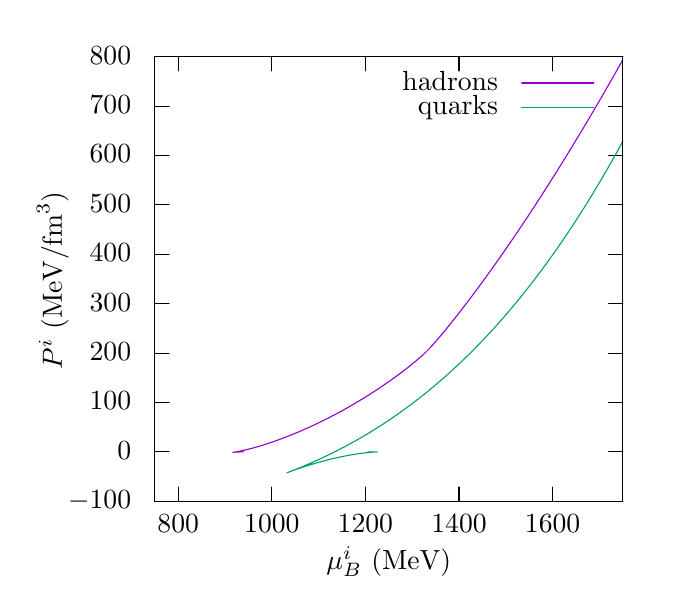
\begin{tikzpicture}[gnuplot]
%% generated with GNUPLOT 5.0p4 (Lua 5.2; terminal rev. 99, script rev. 100)
%% Wed Oct 26 17:32:28 2016
\path (0.000,0.000) rectangle (8.000,7.000);
\gpcolor{color=gp lt color border}
\gpsetlinetype{gp lt border}
\gpsetdashtype{gp dt solid}
\gpsetlinewidth{1.00}
\draw[gp path] (1.504,0.985)--(1.684,0.985);
\draw[gp path] (7.447,0.985)--(7.267,0.985);
\node[gp node right] at (1.320,0.985) {$-100$};
\draw[gp path] (1.504,1.612)--(1.684,1.612);
\draw[gp path] (7.447,1.612)--(7.267,1.612);
\node[gp node right] at (1.320,1.612) {$0$};
\draw[gp path] (1.504,2.240)--(1.684,2.240);
\draw[gp path] (7.447,2.240)--(7.267,2.240);
\node[gp node right] at (1.320,2.240) {$100$};
\draw[gp path] (1.504,2.867)--(1.684,2.867);
\draw[gp path] (7.447,2.867)--(7.267,2.867);
\node[gp node right] at (1.320,2.867) {$200$};
\draw[gp path] (1.504,3.494)--(1.684,3.494);
\draw[gp path] (7.447,3.494)--(7.267,3.494);
\node[gp node right] at (1.320,3.494) {$300$};
\draw[gp path] (1.504,4.122)--(1.684,4.122);
\draw[gp path] (7.447,4.122)--(7.267,4.122);
\node[gp node right] at (1.320,4.122) {$400$};
\draw[gp path] (1.504,4.749)--(1.684,4.749);
\draw[gp path] (7.447,4.749)--(7.267,4.749);
\node[gp node right] at (1.320,4.749) {$500$};
\draw[gp path] (1.504,5.376)--(1.684,5.376);
\draw[gp path] (7.447,5.376)--(7.267,5.376);
\node[gp node right] at (1.320,5.376) {$600$};
\draw[gp path] (1.504,6.004)--(1.684,6.004);
\draw[gp path] (7.447,6.004)--(7.267,6.004);
\node[gp node right] at (1.320,6.004) {$700$};
\draw[gp path] (1.504,6.631)--(1.684,6.631);
\draw[gp path] (7.447,6.631)--(7.267,6.631);
\node[gp node right] at (1.320,6.631) {$800$};
\draw[gp path] (1.801,0.985)--(1.801,1.165);
\draw[gp path] (1.801,6.631)--(1.801,6.451);
\node[gp node center] at (1.801,0.677) {$800$};
\draw[gp path] (2.990,0.985)--(2.990,1.165);
\draw[gp path] (2.990,6.631)--(2.990,6.451);
\node[gp node center] at (2.990,0.677) {$1000$};
\draw[gp path] (4.178,0.985)--(4.178,1.165);
\draw[gp path] (4.178,6.631)--(4.178,6.451);
\node[gp node center] at (4.178,0.677) {$1200$};
\draw[gp path] (5.367,0.985)--(5.367,1.165);
\draw[gp path] (5.367,6.631)--(5.367,6.451);
\node[gp node center] at (5.367,0.677) {$1400$};
\draw[gp path] (6.556,0.985)--(6.556,1.165);
\draw[gp path] (6.556,6.631)--(6.556,6.451);
\node[gp node center] at (6.556,0.677) {$1600$};
\draw[gp path] (1.504,6.631)--(1.504,0.985)--(7.447,0.985)--(7.447,6.631)--cycle;
\node[gp node center,rotate=-270] at (0.246,3.808) {$P^i$ ($\rm{MeV}/\rm{fm}^3$)};
\node[gp node center] at (4.475,0.215) {$\mu_B^i$ (MeV)};
\node[gp node right] at (5.979,6.297) {hadrons};
\gpcolor{rgb color={0.580,0.000,0.827}}
\draw[gp path] (6.163,6.297)--(7.079,6.297);
\draw[gp path] (2.630,1.612)--(2.629,1.612)--(2.628,1.612)--(2.627,1.612)--(2.626,1.612)%
  --(2.625,1.612)--(2.624,1.612)--(2.623,1.612)--(2.622,1.612)--(2.620,1.612)--(2.619,1.612)%
  --(2.618,1.612)--(2.616,1.612)--(2.615,1.612)--(2.613,1.612)--(2.612,1.612)--(2.610,1.612)%
  --(2.609,1.612)--(2.608,1.612)--(2.606,1.612)--(2.605,1.612)--(2.603,1.612)--(2.602,1.612)%
  --(2.600,1.612)--(2.599,1.612)--(2.597,1.612)--(2.596,1.612)--(2.594,1.612)--(2.593,1.612)%
  --(2.591,1.612)--(2.590,1.612)--(2.589,1.612)--(2.587,1.612)--(2.586,1.612)--(2.584,1.612)%
  --(2.583,1.612)--(2.582,1.612)--(2.580,1.612)--(2.579,1.612)--(2.577,1.611)--(2.576,1.611)%
  --(2.575,1.611)--(2.573,1.611)--(2.572,1.611)--(2.571,1.611)--(2.569,1.611)--(2.568,1.611)%
  --(2.567,1.611)--(2.565,1.611)--(2.564,1.611)--(2.563,1.611)--(2.561,1.611)--(2.560,1.611)%
  --(2.559,1.611)--(2.558,1.611)--(2.556,1.611)--(2.555,1.611)--(2.554,1.611)--(2.553,1.611)%
  --(2.552,1.611)--(2.550,1.611)--(2.549,1.610)--(2.548,1.610)--(2.547,1.610)--(2.546,1.610)%
  --(2.545,1.610)--(2.544,1.610)--(2.543,1.610)--(2.542,1.610)--(2.540,1.610)--(2.539,1.610)%
  --(2.538,1.610)--(2.537,1.610)--(2.536,1.610)--(2.535,1.610)--(2.534,1.610)--(2.533,1.610)%
  --(2.532,1.610)--(2.531,1.610)--(2.530,1.609)--(2.529,1.609)--(2.528,1.609)--(2.527,1.609)%
  --(2.526,1.609)--(2.525,1.609)--(2.524,1.609)--(2.523,1.609)--(2.522,1.609)--(2.521,1.609)%
  --(2.520,1.609)--(2.519,1.609)--(2.518,1.609)--(2.517,1.609)--(2.516,1.609)--(2.515,1.609)%
  --(2.515,1.608)--(2.514,1.608)--(2.513,1.608)--(2.512,1.608)--(2.511,1.608)--(2.510,1.608)%
  --(2.509,1.608)--(2.508,1.608)--(2.507,1.608)--(2.506,1.608)--(2.505,1.608)--(2.504,1.608)%
  --(2.503,1.608)--(2.502,1.608)--(2.502,1.607)--(2.501,1.607)--(2.500,1.607)--(2.499,1.607)%
  --(2.498,1.607)--(2.497,1.607)--(2.496,1.607)--(2.495,1.607)--(2.494,1.607)--(2.495,1.607)%
  --(2.496,1.607)--(2.497,1.607)--(2.498,1.607)--(2.499,1.607)--(2.500,1.607)--(2.500,1.608)%
  --(2.501,1.608)--(2.502,1.608)--(2.503,1.608)--(2.504,1.608)--(2.505,1.608)--(2.506,1.608)%
  --(2.507,1.608)--(2.507,1.609)--(2.508,1.609)--(2.509,1.609)--(2.510,1.609)--(2.511,1.609)%
  --(2.512,1.609)--(2.513,1.609)--(2.514,1.610)--(2.515,1.610)--(2.516,1.610)--(2.517,1.610)%
  --(2.518,1.610)--(2.519,1.610)--(2.520,1.611)--(2.521,1.611)--(2.522,1.611)--(2.523,1.611)%
  --(2.524,1.611)--(2.525,1.611)--(2.526,1.611)--(2.526,1.612)--(2.527,1.612)--(2.528,1.612)%
  --(2.529,1.612)--(2.530,1.612)--(2.531,1.612)--(2.532,1.612)--(2.533,1.613)--(2.534,1.613)%
  --(2.535,1.613)--(2.536,1.613)--(2.537,1.613)--(2.538,1.614)--(2.539,1.614)--(2.540,1.614)%
  --(2.541,1.614)--(2.542,1.614)--(2.543,1.614)--(2.544,1.615)--(2.545,1.615)--(2.546,1.615)%
  --(2.547,1.615)--(2.548,1.615)--(2.549,1.616)--(2.550,1.616)--(2.551,1.616)--(2.553,1.616)%
  --(2.554,1.616)--(2.555,1.617)--(2.556,1.617)--(2.557,1.617)--(2.558,1.617)--(2.559,1.617)%
  --(2.560,1.618)--(2.562,1.618)--(2.563,1.618)--(2.564,1.618)--(2.565,1.619)--(2.566,1.619)%
  --(2.568,1.619)--(2.569,1.619)--(2.570,1.619)--(2.571,1.620)--(2.573,1.620)--(2.574,1.620)%
  --(2.575,1.620)--(2.576,1.621)--(2.578,1.621)--(2.579,1.621)--(2.580,1.621)--(2.582,1.622)%
  --(2.583,1.622)--(2.584,1.622)--(2.586,1.623)--(2.587,1.623)--(2.588,1.623)--(2.590,1.623)%
  --(2.591,1.624)--(2.592,1.624)--(2.594,1.624)--(2.595,1.625)--(2.597,1.625)--(2.598,1.625)%
  --(2.599,1.625)--(2.601,1.626)--(2.602,1.626)--(2.604,1.626)--(2.605,1.627)--(2.607,1.627)%
  --(2.608,1.627)--(2.610,1.628)--(2.611,1.628)--(2.613,1.628)--(2.614,1.629)--(2.616,1.629)%
  --(2.617,1.629)--(2.619,1.630)--(2.620,1.630)--(2.622,1.630)--(2.623,1.631)--(2.625,1.631)%
  --(2.627,1.631)--(2.628,1.632)--(2.630,1.632)--(2.631,1.632)--(2.633,1.633)--(2.635,1.633)%
  --(2.636,1.634)--(2.638,1.634)--(2.640,1.634)--(2.641,1.635)--(2.643,1.635)--(2.645,1.635)%
  --(2.646,1.636)--(2.648,1.636)--(2.650,1.637)--(2.651,1.637)--(2.653,1.637)--(2.655,1.638)%
  --(2.656,1.638)--(2.658,1.639)--(2.660,1.639)--(2.662,1.639)--(2.663,1.640)--(2.665,1.640)%
  --(2.667,1.641)--(2.669,1.641)--(2.671,1.642)--(2.672,1.642)--(2.674,1.642)--(2.676,1.643)%
  --(2.678,1.643)--(2.680,1.644)--(2.681,1.644)--(2.683,1.645)--(2.685,1.645)--(2.687,1.646)%
  --(2.689,1.646)--(2.691,1.646)--(2.693,1.647)--(2.694,1.647)--(2.696,1.648)--(2.698,1.648)%
  --(2.700,1.649)--(2.702,1.649)--(2.704,1.650)--(2.706,1.650)--(2.708,1.651)--(2.710,1.651)%
  --(2.712,1.652)--(2.714,1.652)--(2.716,1.653)--(2.718,1.653)--(2.720,1.654)--(2.722,1.654)%
  --(2.724,1.655)--(2.726,1.655)--(2.728,1.656)--(2.730,1.656)--(2.732,1.657)--(2.734,1.658)%
  --(2.736,1.658)--(2.738,1.659)--(2.740,1.659)--(2.742,1.660)--(2.744,1.660)--(2.746,1.661)%
  --(2.748,1.661)--(2.750,1.662)--(2.752,1.662)--(2.754,1.663)--(2.756,1.664)--(2.758,1.664)%
  --(2.761,1.665)--(2.763,1.665)--(2.765,1.666)--(2.767,1.667)--(2.769,1.667)--(2.771,1.668)%
  --(2.773,1.668)--(2.776,1.669)--(2.778,1.670)--(2.780,1.670)--(2.782,1.671)--(2.784,1.671)%
  --(2.786,1.672)--(2.789,1.673)--(2.791,1.673)--(2.793,1.674)--(2.795,1.674)--(2.797,1.675)%
  --(2.800,1.676)--(2.802,1.676)--(2.804,1.677)--(2.806,1.678)--(2.809,1.678)--(2.811,1.679)%
  --(2.813,1.680)--(2.815,1.680)--(2.818,1.681)--(2.820,1.682)--(2.822,1.682)--(2.825,1.683)%
  --(2.827,1.684)--(2.829,1.684)--(2.831,1.685)--(2.834,1.686)--(2.836,1.686)--(2.838,1.687)%
  --(2.841,1.688)--(2.843,1.689)--(2.845,1.689)--(2.848,1.690)--(2.850,1.691)--(2.853,1.691)%
  --(2.855,1.692)--(2.857,1.693)--(2.860,1.694)--(2.862,1.694)--(2.864,1.695)--(2.867,1.696)%
  --(2.869,1.696)--(2.872,1.697)--(2.874,1.698)--(2.876,1.699)--(2.879,1.699)--(2.881,1.700)%
  --(2.884,1.701)--(2.886,1.702)--(2.889,1.702)--(2.891,1.703)--(2.894,1.704)--(2.896,1.705)%
  --(2.899,1.706)--(2.901,1.706)--(2.903,1.707)--(2.906,1.708)--(2.908,1.709)--(2.911,1.710)%
  --(2.913,1.710)--(2.916,1.711)--(2.918,1.712)--(2.921,1.713)--(2.923,1.714)--(2.926,1.714)%
  --(2.929,1.715)--(2.931,1.716)--(2.934,1.717)--(2.936,1.718)--(2.939,1.719)--(2.941,1.719)%
  --(2.944,1.720)--(2.946,1.721)--(2.949,1.722)--(2.951,1.723)--(2.954,1.724)--(2.957,1.724)%
  --(2.959,1.725)--(2.962,1.726)--(2.964,1.727)--(2.967,1.728)--(2.970,1.729)--(2.972,1.730)%
  --(2.975,1.731)--(2.977,1.731)--(2.980,1.732)--(2.983,1.733)--(2.985,1.734)--(2.988,1.735)%
  --(2.991,1.736)--(2.993,1.737)--(2.996,1.738)--(2.999,1.739)--(3.001,1.740)--(3.004,1.740)%
  --(3.007,1.741)--(3.009,1.742)--(3.012,1.743)--(3.015,1.744)--(3.017,1.745)--(3.020,1.746)%
  --(3.023,1.747)--(3.025,1.748)--(3.028,1.749)--(3.031,1.750)--(3.034,1.751)--(3.036,1.752)%
  --(3.039,1.753)--(3.042,1.754)--(3.044,1.755)--(3.047,1.756)--(3.050,1.757)--(3.053,1.758)%
  --(3.055,1.759)--(3.058,1.760)--(3.061,1.761)--(3.064,1.762)--(3.066,1.763)--(3.069,1.764)%
  --(3.072,1.765)--(3.075,1.766)--(3.077,1.767)--(3.080,1.768)--(3.083,1.769)--(3.086,1.770)%
  --(3.089,1.771)--(3.091,1.772)--(3.094,1.773)--(3.097,1.774)--(3.100,1.775)--(3.103,1.776)%
  --(3.105,1.777)--(3.108,1.778)--(3.111,1.779)--(3.114,1.780)--(3.117,1.781)--(3.120,1.782)%
  --(3.122,1.783)--(3.125,1.784)--(3.128,1.785)--(3.131,1.786)--(3.134,1.787)--(3.137,1.789)%
  --(3.139,1.790)--(3.142,1.791)--(3.145,1.792)--(3.148,1.793)--(3.151,1.794)--(3.154,1.795)%
  --(3.157,1.796)--(3.160,1.797)--(3.162,1.798)--(3.165,1.799)--(3.168,1.801)--(3.171,1.802)%
  --(3.174,1.803)--(3.177,1.804)--(3.180,1.805)--(3.183,1.806)--(3.186,1.807)--(3.188,1.808)%
  --(3.191,1.810)--(3.194,1.811)--(3.197,1.812)--(3.200,1.813)--(3.203,1.814)--(3.206,1.815)%
  --(3.209,1.817)--(3.212,1.818)--(3.215,1.819)--(3.218,1.820)--(3.221,1.821)--(3.224,1.822)%
  --(3.226,1.824)--(3.229,1.825)--(3.232,1.826)--(3.235,1.827)--(3.238,1.828)--(3.241,1.830)%
  --(3.244,1.831)--(3.247,1.832)--(3.250,1.833)--(3.253,1.834)--(3.256,1.836)--(3.259,1.837)%
  --(3.262,1.838)--(3.265,1.839)--(3.268,1.840)--(3.271,1.842)--(3.274,1.843)--(3.277,1.844)%
  --(3.280,1.845)--(3.283,1.847)--(3.286,1.848)--(3.289,1.849)--(3.292,1.850)--(3.295,1.852)%
  --(3.298,1.853)--(3.301,1.854)--(3.304,1.855)--(3.307,1.857)--(3.310,1.858)--(3.313,1.859)%
  --(3.316,1.860)--(3.319,1.862)--(3.322,1.863)--(3.325,1.864)--(3.328,1.865)--(3.331,1.867)%
  --(3.334,1.868)--(3.337,1.869)--(3.340,1.871)--(3.343,1.872)--(3.346,1.873)--(3.349,1.875)%
  --(3.352,1.876)--(3.355,1.877)--(3.358,1.878)--(3.361,1.880)--(3.365,1.881)--(3.368,1.882)%
  --(3.371,1.884)--(3.374,1.885)--(3.377,1.886)--(3.380,1.888)--(3.383,1.889)--(3.386,1.890)%
  --(3.389,1.892)--(3.392,1.893)--(3.395,1.894)--(3.398,1.896)--(3.401,1.897)--(3.404,1.899)%
  --(3.407,1.900)--(3.410,1.901)--(3.413,1.903)--(3.417,1.904)--(3.420,1.905)--(3.423,1.907)%
  --(3.426,1.908)--(3.429,1.909)--(3.432,1.911)--(3.435,1.912)--(3.438,1.914)--(3.441,1.915)%
  --(3.444,1.916)--(3.447,1.918)--(3.450,1.919)--(3.454,1.921)--(3.457,1.922)--(3.460,1.923)%
  --(3.463,1.925)--(3.466,1.926)--(3.469,1.928)--(3.472,1.929)--(3.475,1.930)--(3.478,1.932)%
  --(3.481,1.933)--(3.485,1.935)--(3.488,1.936)--(3.491,1.938)--(3.494,1.939)--(3.497,1.940)%
  --(3.500,1.942)--(3.503,1.943)--(3.506,1.945)--(3.509,1.946)--(3.512,1.948)--(3.516,1.949)%
  --(3.519,1.951)--(3.522,1.952)--(3.525,1.954)--(3.528,1.955)--(3.531,1.956)--(3.534,1.958)%
  --(3.537,1.959)--(3.540,1.961)--(3.544,1.962)--(3.547,1.964)--(3.550,1.965)--(3.553,1.967)%
  --(3.556,1.968)--(3.559,1.970)--(3.562,1.971)--(3.565,1.973)--(3.569,1.974)--(3.572,1.976)%
  --(3.575,1.977)--(3.578,1.979)--(3.581,1.980)--(3.584,1.982)--(3.587,1.983)--(3.590,1.985)%
  --(3.593,1.986)--(3.597,1.988)--(3.600,1.989)--(3.603,1.991)--(3.606,1.992)--(3.609,1.994)%
  --(3.612,1.995)--(3.615,1.997)--(3.618,1.998)--(3.622,2.000)--(3.625,2.002)--(3.628,2.003)%
  --(3.631,2.005)--(3.634,2.006)--(3.637,2.008)--(3.640,2.009)--(3.643,2.011)--(3.647,2.012)%
  --(3.650,2.014)--(3.653,2.015)--(3.656,2.017)--(3.659,2.019)--(3.662,2.020)--(3.665,2.022)%
  --(3.668,2.023)--(3.672,2.025)--(3.675,2.026)--(3.678,2.028)--(3.681,2.030)--(3.684,2.031)%
  --(3.687,2.033)--(3.690,2.034)--(3.693,2.036)--(3.697,2.037)--(3.700,2.039)--(3.703,2.041)%
  --(3.706,2.042)--(3.709,2.044)--(3.712,2.045)--(3.715,2.047)--(3.718,2.049)--(3.722,2.050)%
  --(3.725,2.052)--(3.728,2.053)--(3.731,2.055)--(3.734,2.057)--(3.737,2.058)--(3.740,2.060)%
  --(3.743,2.061)--(3.746,2.063)--(3.750,2.065)--(3.753,2.066)--(3.756,2.068)--(3.759,2.070)%
  --(3.762,2.071)--(3.765,2.073)--(3.768,2.074)--(3.771,2.076)--(3.774,2.078)--(3.778,2.079)%
  --(3.781,2.081)--(3.784,2.083)--(3.787,2.084)--(3.790,2.086)--(3.793,2.088)--(3.796,2.089)%
  --(3.799,2.091)--(3.802,2.092)--(3.805,2.094)--(3.809,2.096)--(3.812,2.097)--(3.815,2.099)%
  --(3.818,2.101)--(3.821,2.102)--(3.824,2.104)--(3.827,2.106)--(3.830,2.107)--(3.833,2.109)%
  --(3.836,2.111)--(3.839,2.112)--(3.842,2.114)--(3.846,2.116)--(3.849,2.117)--(3.852,2.119)%
  --(3.855,2.121)--(3.858,2.122)--(3.861,2.124)--(3.864,2.126)--(3.867,2.127)--(3.870,2.129)%
  --(3.873,2.131)--(3.876,2.132)--(3.879,2.134)--(3.882,2.136)--(3.885,2.138)--(3.889,2.139)%
  --(3.892,2.141)--(3.895,2.143)--(3.898,2.144)--(3.901,2.146)--(3.904,2.148)--(3.907,2.149)%
  --(3.910,2.151)--(3.913,2.153)--(3.916,2.154)--(3.919,2.156)--(3.922,2.158)--(3.925,2.160)%
  --(3.928,2.161)--(3.931,2.163)--(3.934,2.165)--(3.937,2.166)--(3.940,2.168)--(3.943,2.170)%
  --(3.946,2.172)--(3.949,2.173)--(3.952,2.175)--(3.955,2.177)--(3.958,2.178)--(3.962,2.180)%
  --(3.965,2.182)--(3.968,2.184)--(3.971,2.185)--(3.974,2.187)--(3.977,2.189)--(3.980,2.190)%
  --(3.983,2.192)--(3.986,2.194)--(3.989,2.196)--(3.992,2.197)--(3.995,2.199)--(3.998,2.201)%
  --(4.001,2.203)--(4.004,2.204)--(4.007,2.206)--(4.010,2.208)--(4.013,2.209)--(4.015,2.211)%
  --(4.018,2.213)--(4.021,2.215)--(4.024,2.216)--(4.027,2.218)--(4.030,2.220)--(4.033,2.222)%
  --(4.036,2.223)--(4.039,2.225)--(4.042,2.227)--(4.045,2.229)--(4.048,2.230)--(4.051,2.232)%
  --(4.054,2.234)--(4.057,2.235)--(4.060,2.237)--(4.063,2.239)--(4.066,2.241)--(4.069,2.242)%
  --(4.072,2.244)--(4.075,2.246)--(4.077,2.248)--(4.080,2.249)--(4.083,2.251)--(4.086,2.253)%
  --(4.089,2.255)--(4.092,2.256)--(4.095,2.258)--(4.098,2.260)--(4.101,2.262)--(4.104,2.263)%
  --(4.107,2.265)--(4.110,2.267)--(4.112,2.269)--(4.115,2.270)--(4.118,2.272)--(4.121,2.274)%
  --(4.124,2.276)--(4.127,2.277)--(4.130,2.279)--(4.133,2.281)--(4.135,2.283)--(4.138,2.284)%
  --(4.141,2.286)--(4.144,2.288)--(4.147,2.290)--(4.150,2.291)--(4.153,2.293)--(4.155,2.295)%
  --(4.158,2.297)--(4.161,2.298)--(4.164,2.300)--(4.167,2.302)--(4.170,2.304)--(4.172,2.305)%
  --(4.175,2.307)--(4.178,2.309)--(4.181,2.311)--(4.184,2.312)--(4.187,2.314)--(4.189,2.316)%
  --(4.192,2.318)--(4.195,2.319)--(4.198,2.321)--(4.201,2.323)--(4.203,2.325)--(4.206,2.326)%
  --(4.209,2.328)--(4.212,2.330)--(4.214,2.332)--(4.217,2.333)--(4.220,2.335)--(4.223,2.337)%
  --(4.226,2.339)--(4.228,2.340)--(4.231,2.342)--(4.234,2.344)--(4.237,2.346)--(4.239,2.347)%
  --(4.242,2.349)--(4.245,2.351)--(4.248,2.353)--(4.250,2.354)--(4.253,2.356)--(4.256,2.358)%
  --(4.258,2.360)--(4.261,2.361)--(4.264,2.363)--(4.267,2.365)--(4.269,2.367)--(4.272,2.368)%
  --(4.275,2.370)--(4.277,2.372)--(4.280,2.374)--(4.283,2.375)--(4.285,2.377)--(4.288,2.379)%
  --(4.291,2.380)--(4.293,2.382)--(4.296,2.384)--(4.299,2.386)--(4.301,2.387)--(4.304,2.389)%
  --(4.307,2.391)--(4.309,2.393)--(4.312,2.394)--(4.315,2.396)--(4.317,2.398)--(4.320,2.400)%
  --(4.322,2.401)--(4.325,2.403)--(4.328,2.405)--(4.330,2.406)--(4.333,2.408)--(4.336,2.410)%
  --(4.338,2.412)--(4.341,2.413)--(4.343,2.415)--(4.346,2.417)--(4.348,2.418)--(4.351,2.420)%
  --(4.354,2.422)--(4.356,2.424)--(4.359,2.425)--(4.361,2.427)--(4.364,2.429)--(4.366,2.430)%
  --(4.369,2.432)--(4.372,2.434)--(4.374,2.436)--(4.377,2.437)--(4.379,2.439)--(4.382,2.441)%
  --(4.384,2.442)--(4.387,2.444)--(4.389,2.446)--(4.392,2.447)--(4.394,2.449)--(4.397,2.451)%
  --(4.399,2.453)--(4.402,2.454)--(4.404,2.456)--(4.407,2.458)--(4.409,2.459)--(4.412,2.461)%
  --(4.414,2.463)--(4.416,2.464)--(4.419,2.466)--(4.421,2.468)--(4.424,2.469)--(4.426,2.471)%
  --(4.429,2.473)--(4.431,2.474)--(4.434,2.476)--(4.436,2.478)--(4.438,2.479)--(4.441,2.481)%
  --(4.443,2.483)--(4.446,2.484)--(4.448,2.486)--(4.450,2.488)--(4.453,2.489)--(4.455,2.491)%
  --(4.458,2.493)--(4.460,2.494)--(4.462,2.496)--(4.465,2.498)--(4.467,2.499)--(4.469,2.501)%
  --(4.472,2.503)--(4.474,2.504)--(4.476,2.506)--(4.479,2.507)--(4.481,2.509)--(4.483,2.511)%
  --(4.486,2.512)--(4.488,2.514)--(4.490,2.516)--(4.493,2.517)--(4.495,2.519)--(4.497,2.520)%
  --(4.499,2.522)--(4.502,2.524)--(4.504,2.525)--(4.506,2.527)--(4.509,2.529)--(4.511,2.530)%
  --(4.513,2.532)--(4.515,2.533)--(4.518,2.535)--(4.520,2.537)--(4.522,2.538)--(4.524,2.540)%
  --(4.526,2.541)--(4.529,2.543)--(4.531,2.545)--(4.533,2.546)--(4.535,2.548)--(4.537,2.549)%
  --(4.540,2.551)--(4.542,2.552)--(4.544,2.554)--(4.546,2.556)--(4.548,2.557)--(4.551,2.559)%
  --(4.553,2.560)--(4.555,2.562)--(4.557,2.563)--(4.559,2.565)--(4.561,2.566)--(4.563,2.568)%
  --(4.565,2.570)--(4.568,2.571)--(4.570,2.573)--(4.572,2.574)--(4.574,2.576)--(4.576,2.577)%
  --(4.578,2.579)--(4.580,2.580)--(4.582,2.582)--(4.584,2.583)--(4.586,2.585)--(4.588,2.586)%
  --(4.591,2.588)--(4.593,2.589)--(4.595,2.591)--(4.597,2.593)--(4.599,2.594)--(4.601,2.596)%
  --(4.603,2.597)--(4.605,2.599)--(4.607,2.600)--(4.609,2.602)--(4.611,2.603)--(4.613,2.604)%
  --(4.615,2.606)--(4.617,2.607)--(4.619,2.609)--(4.621,2.610)--(4.623,2.612)--(4.625,2.613)%
  --(4.627,2.615)--(4.629,2.616)--(4.630,2.618)--(4.632,2.619)--(4.634,2.621)--(4.636,2.622)%
  --(4.638,2.624)--(4.640,2.625)--(4.642,2.626)--(4.644,2.628)--(4.646,2.629)--(4.648,2.631)%
  --(4.650,2.632)--(4.651,2.634)--(4.653,2.635)--(4.655,2.636)--(4.657,2.638)--(4.659,2.639)%
  --(4.661,2.641)--(4.663,2.642)--(4.664,2.643)--(4.666,2.645)--(4.668,2.646)--(4.670,2.648)%
  --(4.672,2.649)--(4.673,2.650)--(4.675,2.652)--(4.677,2.653)--(4.679,2.655)--(4.681,2.656)%
  --(4.682,2.657)--(4.684,2.659)--(4.686,2.660)--(4.688,2.661)--(4.689,2.663)--(4.691,2.664)%
  --(4.693,2.665)--(4.695,2.667)--(4.696,2.668)--(4.698,2.669)--(4.700,2.671)--(4.702,2.672)%
  --(4.703,2.673)--(4.705,2.675)--(4.707,2.676)--(4.708,2.677)--(4.710,2.679)--(4.712,2.680)%
  --(4.713,2.681)--(4.715,2.683)--(4.717,2.684)--(4.718,2.685)--(4.720,2.687)--(4.722,2.688)%
  --(4.723,2.689)--(4.725,2.690)--(4.726,2.692)--(4.728,2.693)--(4.730,2.694)--(4.731,2.695)%
  --(4.733,2.697)--(4.734,2.698)--(4.736,2.699)--(4.738,2.701)--(4.739,2.702)--(4.741,2.703)%
  --(4.742,2.704)--(4.744,2.705)--(4.745,2.707)--(4.747,2.708)--(4.748,2.709)--(4.750,2.710)%
  --(4.751,2.712)--(4.753,2.713)--(4.754,2.714)--(4.756,2.715)--(4.757,2.716)--(4.759,2.718)%
  --(4.760,2.719)--(4.762,2.720)--(4.763,2.721)--(4.765,2.722)--(4.766,2.723)--(4.768,2.725)%
  --(4.769,2.726)--(4.770,2.727)--(4.772,2.728)--(4.773,2.729)--(4.775,2.730)--(4.776,2.732)%
  --(4.778,2.733)--(4.779,2.734)--(4.780,2.735)--(4.782,2.736)--(4.783,2.737)--(4.784,2.738)%
  --(4.786,2.740)--(4.787,2.741)--(4.789,2.742)--(4.790,2.743)--(4.791,2.744)--(4.793,2.745)%
  --(4.794,2.746)--(4.795,2.747)--(4.797,2.748)--(4.798,2.749)--(4.799,2.750)--(4.800,2.752)%
  --(4.802,2.753)--(4.803,2.754)--(4.804,2.755)--(4.806,2.756)--(4.807,2.757)--(4.808,2.758)%
  --(4.809,2.759)--(4.811,2.760)--(4.812,2.761)--(4.813,2.762)--(4.814,2.763)--(4.816,2.764)%
  --(4.817,2.765)--(4.818,2.766)--(4.819,2.767)--(4.820,2.768)--(4.822,2.769)--(4.823,2.770)%
  --(4.824,2.771)--(4.825,2.772)--(4.826,2.773)--(4.827,2.774)--(4.829,2.775)--(4.830,2.776)%
  --(4.831,2.777)--(4.832,2.778)--(4.833,2.779)--(4.834,2.780)--(4.835,2.781)--(4.836,2.782)%
  --(4.838,2.783)--(4.839,2.784)--(4.840,2.784)--(4.841,2.785)--(4.842,2.786)--(4.843,2.787)%
  --(4.844,2.788)--(4.845,2.789)--(4.846,2.790)--(4.847,2.791)--(4.848,2.792)--(4.849,2.793)%
  --(4.850,2.793)--(4.851,2.794)--(4.852,2.795)--(4.853,2.796)--(4.854,2.797)--(4.855,2.798)%
  --(4.856,2.799)--(4.857,2.800)--(4.858,2.800)--(4.859,2.801)--(4.860,2.802)--(4.861,2.803)%
  --(4.862,2.804)--(4.863,2.805)--(4.864,2.805)--(4.865,2.806)--(4.866,2.807)--(4.867,2.808)%
  --(4.868,2.809)--(4.869,2.809)--(4.870,2.810)--(4.871,2.811)--(4.872,2.812)--(4.872,2.813)%
  --(4.873,2.813)--(4.874,2.814)--(4.875,2.815)--(4.876,2.816)--(4.877,2.816)--(4.878,2.817)%
  --(4.879,2.818)--(4.879,2.819)--(4.880,2.819)--(4.881,2.820)--(4.882,2.821)--(4.883,2.822)%
  --(4.884,2.822)--(4.884,2.823)--(4.885,2.824)--(4.886,2.825)--(4.887,2.825)--(4.888,2.826)%
  --(4.888,2.827)--(4.889,2.827)--(4.890,2.828)--(4.891,2.829)--(4.892,2.829)--(4.892,2.830)%
  --(4.893,2.831)--(4.894,2.831)--(4.895,2.832)--(4.895,2.833)--(4.896,2.833)--(4.897,2.834)%
  --(4.897,2.835)--(4.898,2.835)--(4.899,2.836)--(4.900,2.837)--(4.901,2.838)--(4.902,2.839)%
  --(4.903,2.840)--(4.904,2.840)--(4.904,2.841)--(4.905,2.842)--(4.906,2.842)--(4.906,2.843)%
  --(4.907,2.843)--(4.908,2.844)--(4.908,2.845)--(4.909,2.845)--(4.910,2.846)--(4.911,2.847)%
  --(4.912,2.847)--(4.912,2.848)--(4.913,2.848)--(4.913,2.849)--(4.914,2.850)--(4.915,2.850)%
  --(4.915,2.851)--(4.916,2.851)--(4.916,2.852)--(4.917,2.852)--(4.917,2.853)--(4.918,2.853)%
  --(4.919,2.854)--(4.920,2.855)--(4.921,2.856)--(4.922,2.857)--(4.923,2.858)--(4.924,2.859)%
  --(4.925,2.860)--(4.926,2.861)--(4.927,2.862)--(4.928,2.862)--(4.928,2.863)--(4.929,2.863)%
  --(4.929,2.864)--(4.930,2.864)--(4.930,2.865)--(4.931,2.865)--(4.931,2.866)--(4.932,2.866)%
  --(4.933,2.867)--(4.933,2.868)--(4.934,2.868)--(4.935,2.869)--(4.936,2.870)--(4.937,2.871)%
  --(4.938,2.872)--(4.939,2.873)--(4.940,2.873)--(4.940,2.874)--(4.941,2.874)--(4.941,2.875)%
  --(4.942,2.876)--(4.943,2.876)--(4.943,2.877)--(4.944,2.877)--(4.944,2.878)--(4.945,2.878)%
  --(4.945,2.879)--(4.946,2.879)--(4.946,2.880)--(4.947,2.880)--(4.947,2.881)--(4.948,2.881)%
  --(4.948,2.882)--(4.949,2.882)--(4.949,2.883)--(4.950,2.883)--(4.950,2.884)--(4.951,2.884)%
  --(4.951,2.885)--(4.952,2.885)--(4.952,2.886)--(4.953,2.886)--(4.953,2.887)--(4.954,2.887)%
  --(4.954,2.888)--(4.955,2.888)--(4.955,2.889)--(4.956,2.889)--(4.956,2.890)--(4.957,2.890)%
  --(4.957,2.891)--(4.958,2.891)--(4.958,2.892)--(4.959,2.892)--(4.959,2.893)--(4.960,2.893)%
  --(4.960,2.894)--(4.961,2.894)--(4.961,2.895)--(4.962,2.895)--(4.962,2.896)--(4.963,2.896)%
  --(4.963,2.897)--(4.964,2.897)--(4.964,2.898)--(4.965,2.898)--(4.965,2.899)--(4.966,2.899)%
  --(4.966,2.900)--(4.967,2.900)--(4.967,2.901)--(4.968,2.901)--(4.968,2.902)--(4.969,2.902)%
  --(4.969,2.903)--(4.970,2.903)--(4.970,2.904)--(4.971,2.904)--(4.971,2.905)--(4.972,2.905)%
  --(4.972,2.906)--(4.973,2.906)--(4.973,2.907)--(4.974,2.907)--(4.974,2.908)--(4.975,2.908)%
  --(4.975,2.909)--(4.976,2.909)--(4.976,2.910)--(4.977,2.910)--(4.977,2.911)--(4.978,2.911)%
  --(4.978,2.912)--(4.979,2.912)--(4.979,2.913)--(4.980,2.913)--(4.980,2.914)--(4.981,2.914)%
  --(4.981,2.915)--(4.982,2.915)--(4.982,2.916)--(4.983,2.917)--(4.984,2.918)--(4.985,2.919)%
  --(4.986,2.920)--(4.987,2.921)--(4.987,2.922)--(4.988,2.922)--(4.989,2.923)--(4.989,2.924)%
  --(4.990,2.924)--(4.990,2.925)--(4.991,2.925)--(4.991,2.926)--(4.992,2.926)--(4.992,2.927)%
  --(4.993,2.927)--(4.993,2.928)--(4.994,2.928)--(4.994,2.929)--(4.995,2.929)--(4.995,2.930)%
  --(4.996,2.930)--(4.996,2.931)--(4.997,2.932)--(4.998,2.933)--(4.999,2.934)--(5.000,2.935)%
  --(5.001,2.936)--(5.001,2.937)--(5.002,2.937)--(5.002,2.938)--(5.003,2.938)--(5.003,2.939)%
  --(5.004,2.939)--(5.005,2.940)--(5.005,2.941)--(5.006,2.941)--(5.006,2.942)--(5.007,2.942)%
  --(5.007,2.943)--(5.008,2.944)--(5.009,2.945)--(5.010,2.946)--(5.011,2.947)--(5.011,2.948)%
  --(5.012,2.948)--(5.013,2.949)--(5.013,2.950)--(5.014,2.950)--(5.015,2.951)--(5.015,2.952)%
  --(5.016,2.952)--(5.016,2.953)--(5.017,2.954)--(5.018,2.954)--(5.018,2.955)--(5.019,2.956)%
  --(5.020,2.957)--(5.021,2.958)--(5.022,2.959)--(5.022,2.960)--(5.023,2.960)--(5.024,2.961)%
  --(5.025,2.962)--(5.025,2.963)--(5.026,2.964)--(5.027,2.964)--(5.027,2.965)--(5.028,2.966)%
  --(5.029,2.967)--(5.030,2.968)--(5.030,2.969)--(5.031,2.969)--(5.032,2.970)--(5.033,2.971)%
  --(5.033,2.972)--(5.034,2.973)--(5.035,2.974)--(5.036,2.975)--(5.037,2.976)--(5.038,2.977)%
  --(5.039,2.978)--(5.040,2.979)--(5.041,2.980)--(5.042,2.981)--(5.042,2.982)--(5.043,2.983)%
  --(5.044,2.984)--(5.045,2.985)--(5.046,2.986)--(5.047,2.987)--(5.048,2.988)--(5.048,2.989)%
  --(5.049,2.990)--(5.050,2.991)--(5.051,2.992)--(5.052,2.993)--(5.053,2.994)--(5.054,2.995)%
  --(5.055,2.996)--(5.056,2.997)--(5.057,2.998)--(5.058,2.999)--(5.058,3.000)--(5.059,3.001)%
  --(5.060,3.003)--(5.061,3.004)--(5.062,3.005)--(5.063,3.006)--(5.064,3.007)--(5.065,3.008)%
  --(5.066,3.009)--(5.067,3.010)--(5.068,3.012)--(5.069,3.013)--(5.070,3.014)--(5.071,3.015)%
  --(5.072,3.016)--(5.073,3.018)--(5.074,3.019)--(5.076,3.020)--(5.077,3.021)--(5.078,3.022)%
  --(5.079,3.024)--(5.080,3.025)--(5.081,3.026)--(5.082,3.027)--(5.083,3.029)--(5.084,3.030)%
  --(5.085,3.031)--(5.086,3.033)--(5.088,3.034)--(5.089,3.035)--(5.090,3.036)--(5.091,3.038)%
  --(5.092,3.039)--(5.093,3.040)--(5.094,3.042)--(5.096,3.043)--(5.097,3.045)--(5.098,3.046)%
  --(5.099,3.047)--(5.100,3.049)--(5.102,3.050)--(5.103,3.052)--(5.104,3.053)--(5.105,3.054)%
  --(5.106,3.056)--(5.108,3.057)--(5.109,3.059)--(5.110,3.060)--(5.111,3.062)--(5.113,3.063)%
  --(5.114,3.065)--(5.115,3.066)--(5.116,3.068)--(5.118,3.069)--(5.119,3.071)--(5.120,3.072)%
  --(5.122,3.074)--(5.123,3.075)--(5.124,3.077)--(5.126,3.078)--(5.127,3.080)--(5.128,3.082)%
  --(5.130,3.083)--(5.131,3.085)--(5.132,3.086)--(5.134,3.088)--(5.135,3.090)--(5.136,3.091)%
  --(5.138,3.093)--(5.139,3.095)--(5.141,3.096)--(5.142,3.098)--(5.143,3.100)--(5.145,3.101)%
  --(5.146,3.103)--(5.148,3.105)--(5.149,3.106)--(5.150,3.108)--(5.152,3.110)--(5.153,3.111)%
  --(5.155,3.113)--(5.156,3.115)--(5.158,3.117)--(5.159,3.119)--(5.161,3.120)--(5.162,3.122)%
  --(5.164,3.124)--(5.165,3.126)--(5.167,3.127)--(5.168,3.129)--(5.170,3.131)--(5.171,3.133)%
  --(5.173,3.135)--(5.174,3.137)--(5.176,3.138)--(5.177,3.140)--(5.179,3.142)--(5.180,3.144)%
  --(5.182,3.146)--(5.184,3.148)--(5.185,3.150)--(5.187,3.152)--(5.188,3.154)--(5.190,3.156)%
  --(5.192,3.158)--(5.193,3.160)--(5.195,3.161)--(5.196,3.163)--(5.198,3.165)--(5.200,3.167)%
  --(5.201,3.169)--(5.203,3.171)--(5.205,3.173)--(5.206,3.175)--(5.208,3.177)--(5.210,3.180)%
  --(5.211,3.182)--(5.213,3.184)--(5.215,3.186)--(5.216,3.188)--(5.218,3.190)--(5.220,3.192)%
  --(5.221,3.194)--(5.223,3.196)--(5.225,3.198)--(5.227,3.200)--(5.228,3.202)--(5.230,3.205)%
  --(5.232,3.207)--(5.234,3.209)--(5.235,3.211)--(5.237,3.213)--(5.239,3.215)--(5.241,3.218)%
  --(5.242,3.220)--(5.244,3.222)--(5.246,3.224)--(5.248,3.226)--(5.250,3.229)--(5.251,3.231)%
  --(5.253,3.233)--(5.255,3.235)--(5.257,3.238)--(5.259,3.240)--(5.260,3.242)--(5.262,3.244)%
  --(5.264,3.247)--(5.266,3.249)--(5.268,3.251)--(5.270,3.254)--(5.272,3.256)--(5.273,3.258)%
  --(5.275,3.261)--(5.277,3.263)--(5.279,3.265)--(5.281,3.268)--(5.283,3.270)--(5.285,3.273)%
  --(5.287,3.275)--(5.289,3.277)--(5.291,3.280)--(5.292,3.282)--(5.294,3.285)--(5.296,3.287)%
  --(5.298,3.289)--(5.300,3.292)--(5.302,3.294)--(5.304,3.297)--(5.306,3.299)--(5.308,3.302)%
  --(5.310,3.304)--(5.312,3.307)--(5.314,3.309)--(5.316,3.312)--(5.318,3.314)--(5.320,3.317)%
  --(5.322,3.319)--(5.324,3.322)--(5.326,3.324)--(5.328,3.327)--(5.330,3.330)--(5.332,3.332)%
  --(5.334,3.335)--(5.336,3.337)--(5.338,3.340)--(5.340,3.342)--(5.342,3.345)--(5.344,3.348)%
  --(5.346,3.350)--(5.348,3.353)--(5.350,3.356)--(5.353,3.358)--(5.355,3.361)--(5.357,3.364)%
  --(5.359,3.366)--(5.361,3.369)--(5.363,3.372)--(5.365,3.374)--(5.367,3.377)--(5.369,3.380)%
  --(5.371,3.382)--(5.374,3.385)--(5.376,3.388)--(5.378,3.391)--(5.380,3.393)--(5.382,3.396)%
  --(5.384,3.399)--(5.386,3.402)--(5.389,3.404)--(5.391,3.407)--(5.393,3.410)--(5.395,3.413)%
  --(5.397,3.416)--(5.399,3.418)--(5.402,3.421)--(5.404,3.424)--(5.406,3.427)--(5.408,3.430)%
  --(5.410,3.433)--(5.413,3.435)--(5.415,3.438)--(5.417,3.441)--(5.419,3.444)--(5.421,3.447)%
  --(5.424,3.450)--(5.426,3.453)--(5.428,3.456)--(5.430,3.459)--(5.433,3.461)--(5.435,3.464)%
  --(5.437,3.467)--(5.439,3.470)--(5.442,3.473)--(5.444,3.476)--(5.446,3.479)--(5.448,3.482)%
  --(5.451,3.485)--(5.453,3.488)--(5.455,3.491)--(5.458,3.494)--(5.460,3.497)--(5.462,3.500)%
  --(5.465,3.503)--(5.467,3.506)--(5.469,3.509)--(5.471,3.512)--(5.474,3.515)--(5.476,3.518)%
  --(5.478,3.521)--(5.481,3.524)--(5.483,3.528)--(5.485,3.531)--(5.488,3.534)--(5.490,3.537)%
  --(5.492,3.540)--(5.495,3.543)--(5.497,3.546)--(5.500,3.549)--(5.502,3.552)--(5.504,3.556)%
  --(5.507,3.559)--(5.509,3.562)--(5.511,3.565)--(5.514,3.568)--(5.516,3.571)--(5.519,3.575)%
  --(5.521,3.578)--(5.523,3.581)--(5.526,3.584)--(5.528,3.587)--(5.531,3.591)--(5.533,3.594)%
  --(5.535,3.597)--(5.538,3.600)--(5.540,3.603)--(5.543,3.607)--(5.545,3.610)--(5.548,3.613)%
  --(5.550,3.616)--(5.552,3.620)--(5.555,3.623)--(5.557,3.626)--(5.560,3.630)--(5.562,3.633)%
  --(5.565,3.636)--(5.567,3.639)--(5.570,3.643)--(5.572,3.646)--(5.575,3.649)--(5.577,3.653)%
  --(5.580,3.656)--(5.582,3.659)--(5.585,3.663)--(5.587,3.666)--(5.590,3.669)--(5.592,3.673)%
  --(5.595,3.676)--(5.597,3.680)--(5.600,3.683)--(5.602,3.686)--(5.605,3.690)--(5.607,3.693)%
  --(5.610,3.697)--(5.612,3.700)--(5.615,3.703)--(5.617,3.707)--(5.620,3.710)--(5.622,3.714)%
  --(5.625,3.717)--(5.627,3.721)--(5.630,3.724)--(5.632,3.728)--(5.635,3.731)--(5.638,3.735)%
  --(5.640,3.738)--(5.643,3.742)--(5.645,3.745)--(5.648,3.749)--(5.650,3.752)--(5.653,3.756)%
  --(5.656,3.759)--(5.658,3.763)--(5.661,3.766)--(5.663,3.770)--(5.666,3.773)--(5.668,3.777)%
  --(5.671,3.780)--(5.674,3.784)--(5.676,3.788)--(5.679,3.791)--(5.682,3.795)--(5.684,3.798)%
  --(5.687,3.802)--(5.689,3.805)--(5.692,3.809)--(5.695,3.813)--(5.697,3.816)--(5.700,3.820)%
  --(5.702,3.824)--(5.705,3.827)--(5.708,3.831)--(5.710,3.834)--(5.713,3.838)--(5.716,3.842)%
  --(5.718,3.845)--(5.721,3.849)--(5.724,3.853)--(5.726,3.856)--(5.729,3.860)--(5.732,3.864)%
  --(5.734,3.868)--(5.737,3.871)--(5.740,3.875)--(5.742,3.879)--(5.745,3.882)--(5.748,3.886)%
  --(5.750,3.890)--(5.753,3.894)--(5.756,3.897)--(5.758,3.901)--(5.761,3.905)--(5.764,3.909)%
  --(5.766,3.912)--(5.769,3.916)--(5.772,3.920)--(5.775,3.924)--(5.777,3.927)--(5.780,3.931)%
  --(5.783,3.935)--(5.785,3.939)--(5.788,3.943)--(5.791,3.946)--(5.794,3.950)--(5.796,3.954)%
  --(5.799,3.958)--(5.802,3.962)--(5.804,3.966)--(5.807,3.969)--(5.810,3.973)--(5.813,3.977)%
  --(5.815,3.981)--(5.818,3.985)--(5.821,3.989)--(5.824,3.993)--(5.826,3.996)--(5.829,4.000)%
  --(5.832,4.004)--(5.835,4.008)--(5.837,4.012)--(5.840,4.016)--(5.843,4.020)--(5.846,4.024)%
  --(5.848,4.028)--(5.851,4.032)--(5.854,4.036)--(5.857,4.039)--(5.860,4.043)--(5.862,4.047)%
  --(5.865,4.051)--(5.868,4.055)--(5.871,4.059)--(5.873,4.063)--(5.876,4.067)--(5.879,4.071)%
  --(5.882,4.075)--(5.885,4.079)--(5.887,4.083)--(5.890,4.087)--(5.893,4.091)--(5.896,4.095)%
  --(5.899,4.099)--(5.901,4.103)--(5.904,4.107)--(5.907,4.111)--(5.910,4.115)--(5.913,4.119)%
  --(5.915,4.123)--(5.918,4.127)--(5.921,4.131)--(5.924,4.135)--(5.927,4.140)--(5.930,4.144)%
  --(5.932,4.148)--(5.935,4.152)--(5.938,4.156)--(5.941,4.160)--(5.944,4.164)--(5.947,4.168)%
  --(5.949,4.172)--(5.952,4.176)--(5.955,4.180)--(5.958,4.184)--(5.961,4.189)--(5.964,4.193)%
  --(5.967,4.197)--(5.969,4.201)--(5.972,4.205)--(5.975,4.209)--(5.978,4.213)--(5.981,4.218)%
  --(5.984,4.222)--(5.987,4.226)--(5.989,4.230)--(5.992,4.234)--(5.995,4.238)--(5.998,4.243)%
  --(6.001,4.247)--(6.004,4.251)--(6.007,4.255)--(6.010,4.259)--(6.012,4.264)--(6.015,4.268)%
  --(6.018,4.272)--(6.021,4.276)--(6.024,4.280)--(6.027,4.285)--(6.030,4.289)--(6.033,4.293)%
  --(6.036,4.297)--(6.038,4.302)--(6.041,4.306)--(6.044,4.310)--(6.047,4.314)--(6.050,4.319)%
  --(6.053,4.323)--(6.056,4.327)--(6.059,4.331)--(6.062,4.336)--(6.065,4.340)--(6.068,4.344)%
  --(6.070,4.349)--(6.073,4.353)--(6.076,4.357)--(6.079,4.361)--(6.082,4.366)--(6.085,4.370)%
  --(6.088,4.374)--(6.091,4.379)--(6.094,4.383)--(6.097,4.387)--(6.100,4.392)--(6.103,4.396)%
  --(6.106,4.400)--(6.108,4.405)--(6.111,4.409)--(6.114,4.413)--(6.117,4.418)--(6.120,4.422)%
  --(6.123,4.427)--(6.126,4.431)--(6.129,4.435)--(6.132,4.440)--(6.135,4.444)--(6.138,4.448)%
  --(6.141,4.453)--(6.144,4.457)--(6.147,4.462)--(6.150,4.466)--(6.153,4.470)--(6.156,4.475)%
  --(6.159,4.479)--(6.162,4.484)--(6.165,4.488)--(6.168,4.493)--(6.170,4.497)--(6.173,4.501)%
  --(6.176,4.506)--(6.179,4.510)--(6.182,4.515)--(6.185,4.519)--(6.188,4.524)--(6.191,4.528)%
  --(6.194,4.533)--(6.197,4.537)--(6.200,4.542)--(6.203,4.546)--(6.206,4.551)--(6.209,4.555)%
  --(6.212,4.560)--(6.215,4.564)--(6.218,4.569)--(6.221,4.573)--(6.224,4.578)--(6.227,4.582)%
  --(6.230,4.587)--(6.233,4.591)--(6.236,4.596)--(6.239,4.600)--(6.242,4.605)--(6.245,4.609)%
  --(6.248,4.614)--(6.251,4.618)--(6.254,4.623)--(6.257,4.627)--(6.260,4.632)--(6.263,4.637)%
  --(6.266,4.641)--(6.269,4.646)--(6.272,4.650)--(6.275,4.655)--(6.278,4.659)--(6.281,4.664)%
  --(6.284,4.669)--(6.287,4.673)--(6.290,4.678)--(6.293,4.682)--(6.296,4.687)--(6.299,4.692)%
  --(6.302,4.696)--(6.305,4.701)--(6.308,4.705)--(6.311,4.710)--(6.314,4.715)--(6.317,4.719)%
  --(6.320,4.724)--(6.323,4.729)--(6.326,4.733)--(6.330,4.738)--(6.333,4.743)--(6.336,4.747)%
  --(6.339,4.752)--(6.342,4.757)--(6.345,4.761)--(6.348,4.766)--(6.351,4.771)--(6.354,4.775)%
  --(6.357,4.780)--(6.360,4.785)--(6.363,4.789)--(6.366,4.794)--(6.369,4.799)--(6.372,4.803)%
  --(6.375,4.808)--(6.378,4.813)--(6.381,4.818)--(6.384,4.822)--(6.387,4.827)--(6.390,4.832)%
  --(6.393,4.836)--(6.396,4.841)--(6.400,4.846)--(6.403,4.851)--(6.406,4.855)--(6.409,4.860)%
  --(6.412,4.865)--(6.415,4.870)--(6.418,4.874)--(6.421,4.879)--(6.424,4.884)--(6.427,4.889)%
  --(6.430,4.893)--(6.433,4.898)--(6.436,4.903)--(6.439,4.908)--(6.442,4.913)--(6.445,4.917)%
  --(6.449,4.922)--(6.452,4.927)--(6.455,4.932)--(6.458,4.936)--(6.461,4.941)--(6.464,4.946)%
  --(6.467,4.951)--(6.470,4.956)--(6.473,4.961)--(6.476,4.965)--(6.479,4.970)--(6.482,4.975)%
  --(6.485,4.980)--(6.489,4.985)--(6.492,4.990)--(6.495,4.994)--(6.498,4.999)--(6.501,5.004)%
  --(6.504,5.009)--(6.507,5.014)--(6.510,5.019)--(6.513,5.024)--(6.516,5.028)--(6.519,5.033)%
  --(6.522,5.038)--(6.526,5.043)--(6.529,5.048)--(6.532,5.053)--(6.535,5.058)--(6.538,5.063)%
  --(6.541,5.067)--(6.544,5.072)--(6.547,5.077)--(6.550,5.082)--(6.553,5.087)--(6.557,5.092)%
  --(6.560,5.097)--(6.563,5.102)--(6.566,5.107)--(6.569,5.112)--(6.572,5.117)--(6.575,5.122)%
  --(6.578,5.126)--(6.581,5.131)--(6.584,5.136)--(6.588,5.141)--(6.591,5.146)--(6.594,5.151)%
  --(6.597,5.156)--(6.600,5.161)--(6.603,5.166)--(6.606,5.171)--(6.609,5.176)--(6.612,5.181)%
  --(6.616,5.186)--(6.619,5.191)--(6.622,5.196)--(6.625,5.201)--(6.628,5.206)--(6.631,5.211)%
  --(6.634,5.216)--(6.637,5.221)--(6.641,5.226)--(6.644,5.231)--(6.647,5.236)--(6.650,5.241)%
  --(6.653,5.246)--(6.656,5.251)--(6.659,5.256)--(6.662,5.261)--(6.665,5.266)--(6.669,5.271)%
  --(6.672,5.276)--(6.675,5.281)--(6.678,5.286)--(6.681,5.291)--(6.684,5.296)--(6.687,5.301)%
  --(6.691,5.306)--(6.694,5.311)--(6.697,5.317)--(6.700,5.322)--(6.703,5.327)--(6.706,5.332)%
  --(6.709,5.337)--(6.712,5.342)--(6.716,5.347)--(6.719,5.352)--(6.722,5.357)--(6.725,5.362)%
  --(6.728,5.367)--(6.731,5.372)--(6.734,5.378)--(6.738,5.383)--(6.741,5.388)--(6.744,5.393)%
  --(6.747,5.398)--(6.750,5.403)--(6.753,5.408)--(6.756,5.413)--(6.760,5.418)--(6.763,5.424)%
  --(6.766,5.429)--(6.769,5.434)--(6.772,5.439)--(6.775,5.444)--(6.778,5.449)--(6.782,5.454)%
  --(6.785,5.460)--(6.788,5.465)--(6.791,5.470)--(6.794,5.475)--(6.797,5.480)--(6.800,5.485)%
  --(6.804,5.491)--(6.807,5.496)--(6.810,5.501)--(6.813,5.506)--(6.816,5.511)--(6.819,5.516)%
  --(6.822,5.522)--(6.826,5.527)--(6.829,5.532)--(6.832,5.537)--(6.835,5.542)--(6.838,5.548)%
  --(6.841,5.553)--(6.845,5.558)--(6.848,5.563)--(6.851,5.568)--(6.854,5.574)--(6.857,5.579)%
  --(6.860,5.584)--(6.864,5.589)--(6.867,5.595)--(6.870,5.600)--(6.873,5.605)--(6.876,5.610)%
  --(6.879,5.616)--(6.882,5.621)--(6.886,5.626)--(6.889,5.631)--(6.892,5.637)--(6.895,5.642)%
  --(6.898,5.647)--(6.901,5.652)--(6.905,5.658)--(6.908,5.663)--(6.911,5.668)--(6.914,5.673)%
  --(6.917,5.679)--(6.920,5.684)--(6.924,5.689)--(6.927,5.695)--(6.930,5.700)--(6.933,5.705)%
  --(6.936,5.710)--(6.939,5.716)--(6.943,5.721)--(6.946,5.726)--(6.949,5.732)--(6.952,5.737)%
  --(6.955,5.742)--(6.959,5.748)--(6.962,5.753)--(6.965,5.758)--(6.968,5.764)--(6.971,5.769)%
  --(6.974,5.774)--(6.978,5.780)--(6.981,5.785)--(6.984,5.790)--(6.987,5.796)--(6.990,5.801)%
  --(6.993,5.806)--(6.997,5.812)--(7.000,5.817)--(7.003,5.822)--(7.006,5.828)--(7.009,5.833)%
  --(7.013,5.838)--(7.016,5.844)--(7.019,5.849)--(7.022,5.854)--(7.025,5.860)--(7.028,5.865)%
  --(7.032,5.871)--(7.035,5.876)--(7.038,5.881)--(7.041,5.887)--(7.044,5.892)--(7.048,5.898)%
  --(7.051,5.903)--(7.054,5.908)--(7.057,5.914)--(7.060,5.919)--(7.063,5.925)--(7.067,5.930)%
  --(7.070,5.935)--(7.073,5.941)--(7.076,5.946)--(7.079,5.952)--(7.083,5.957)--(7.086,5.963)%
  --(7.089,5.968)--(7.092,5.973)--(7.095,5.979)--(7.099,5.984)--(7.102,5.990)--(7.105,5.995)%
  --(7.108,6.001)--(7.111,6.006)--(7.114,6.012)--(7.118,6.017)--(7.121,6.022)--(7.124,6.028)%
  --(7.127,6.033)--(7.130,6.039)--(7.134,6.044)--(7.137,6.050)--(7.140,6.055)--(7.143,6.061)%
  --(7.146,6.066)--(7.150,6.072)--(7.153,6.077)--(7.156,6.083)--(7.159,6.088)--(7.162,6.094)%
  --(7.166,6.099)--(7.169,6.105)--(7.172,6.110)--(7.175,6.116)--(7.178,6.121)--(7.182,6.127)%
  --(7.185,6.132)--(7.188,6.138)--(7.191,6.143)--(7.194,6.149)--(7.198,6.154)--(7.201,6.160)%
  --(7.204,6.165)--(7.207,6.171)--(7.210,6.177)--(7.214,6.182)--(7.217,6.188)--(7.220,6.193)%
  --(7.223,6.199)--(7.226,6.204)--(7.230,6.210)--(7.233,6.215)--(7.236,6.221)--(7.239,6.226)%
  --(7.242,6.232)--(7.246,6.238)--(7.249,6.243)--(7.252,6.249)--(7.255,6.254)--(7.258,6.260)%
  --(7.262,6.265)--(7.265,6.271)--(7.268,6.277)--(7.271,6.282)--(7.274,6.288)--(7.278,6.293)%
  --(7.281,6.299)--(7.284,6.305)--(7.287,6.310)--(7.290,6.316)--(7.294,6.321)--(7.297,6.327)%
  --(7.300,6.333)--(7.303,6.338)--(7.306,6.344)--(7.310,6.350)--(7.313,6.355)--(7.316,6.361)%
  --(7.319,6.366)--(7.322,6.372)--(7.326,6.378)--(7.329,6.383)--(7.332,6.389)--(7.335,6.395)%
  --(7.339,6.400)--(7.342,6.406)--(7.345,6.412)--(7.348,6.417)--(7.351,6.423)--(7.355,6.429)%
  --(7.358,6.434)--(7.361,6.440)--(7.364,6.446)--(7.367,6.451)--(7.371,6.457)--(7.374,6.463)%
  --(7.377,6.468)--(7.380,6.474)--(7.383,6.480)--(7.387,6.485)--(7.390,6.491)--(7.393,6.497)%
  --(7.396,6.502)--(7.400,6.508)--(7.403,6.514)--(7.406,6.519)--(7.409,6.525)--(7.412,6.531)%
  --(7.416,6.537)--(7.419,6.542)--(7.422,6.548)--(7.425,6.554)--(7.428,6.559)--(7.432,6.565)%
  --(7.435,6.571)--(7.438,6.577)--(7.441,6.582)--(7.445,6.588)--(7.447,6.592);
\gpcolor{color=gp lt color border}
\node[gp node right] at (5.979,5.989) {quarks};
\gpcolor{rgb color={0.000,0.620,0.451}}
\draw[gp path] (6.163,5.989)--(7.079,5.989);
\draw[gp path] (4.207,1.612)--(4.237,1.612)--(4.257,1.612)--(4.272,1.613)--(4.283,1.613)%
  --(4.293,1.613)--(4.301,1.613)--(4.307,1.613)--(4.313,1.613)--(4.317,1.613)--(4.321,1.613)%
  --(4.324,1.613)--(4.327,1.613)--(4.329,1.613)--(4.330,1.613)--(4.331,1.613)--(4.332,1.613)%
  --(4.331,1.613)--(4.330,1.613)--(4.329,1.613)--(4.328,1.613)--(4.326,1.613)--(4.324,1.613)%
  --(4.322,1.613)--(4.320,1.613)--(4.318,1.613)--(4.315,1.613)--(4.312,1.612)--(4.309,1.612)%
  --(4.306,1.612)--(4.304,1.612)--(4.300,1.612)--(4.297,1.611)--(4.293,1.611)--(4.290,1.611)%
  --(4.286,1.611)--(4.282,1.610)--(4.278,1.610)--(4.274,1.610)--(4.270,1.610)--(4.266,1.609)%
  --(4.262,1.609)--(4.258,1.608)--(4.253,1.608)--(4.249,1.608)--(4.244,1.607)--(4.239,1.607)%
  --(4.235,1.606)--(4.230,1.606)--(4.225,1.605)--(4.220,1.605)--(4.215,1.604)--(4.210,1.604)%
  --(4.205,1.603)--(4.200,1.603)--(4.195,1.602)--(4.189,1.602)--(4.184,1.601)--(4.179,1.600)%
  --(4.173,1.600)--(4.168,1.599)--(4.162,1.599)--(4.157,1.598)--(4.151,1.597)--(4.145,1.596)%
  --(4.140,1.596)--(4.134,1.595)--(4.128,1.594)--(4.122,1.593)--(4.116,1.593)--(4.110,1.592)%
  --(4.104,1.591)--(4.098,1.590)--(4.092,1.589)--(4.086,1.588)--(4.080,1.587)--(4.074,1.587)%
  --(4.068,1.586)--(4.062,1.585)--(4.055,1.584)--(4.049,1.583)--(4.043,1.582)--(4.036,1.581)%
  --(4.030,1.580)--(4.024,1.579)--(4.017,1.578)--(4.011,1.576)--(4.004,1.575)--(3.998,1.574)%
  --(3.991,1.573)--(3.984,1.572)--(3.978,1.571)--(3.971,1.570)--(3.965,1.568)--(3.958,1.567)%
  --(3.951,1.566)--(3.944,1.565)--(3.938,1.563)--(3.931,1.562)--(3.924,1.561)--(3.917,1.560)%
  --(3.910,1.558)--(3.904,1.557)--(3.897,1.555)--(3.890,1.554)--(3.883,1.553)--(3.876,1.551)%
  --(3.869,1.550)--(3.862,1.548)--(3.855,1.547)--(3.848,1.545)--(3.841,1.544)--(3.834,1.542)%
  --(3.827,1.541)--(3.819,1.539)--(3.812,1.538)--(3.805,1.536)--(3.798,1.534)--(3.791,1.533)%
  --(3.784,1.531)--(3.776,1.529)--(3.769,1.528)--(3.762,1.526)--(3.755,1.524)--(3.747,1.523)%
  --(3.740,1.521)--(3.733,1.519)--(3.725,1.517)--(3.718,1.515)--(3.711,1.514)--(3.703,1.512)%
  --(3.696,1.510)--(3.688,1.508)--(3.681,1.506)--(3.674,1.504)--(3.666,1.502)--(3.659,1.500)%
  --(3.651,1.498)--(3.644,1.496)--(3.636,1.494)--(3.629,1.492)--(3.621,1.490)--(3.614,1.488)%
  --(3.606,1.486)--(3.598,1.484)--(3.591,1.482)--(3.583,1.480)--(3.576,1.478)--(3.568,1.475)%
  --(3.560,1.473)--(3.553,1.471)--(3.545,1.469)--(3.537,1.467)--(3.530,1.464)--(3.522,1.462)%
  --(3.514,1.460)--(3.507,1.458)--(3.499,1.455)--(3.491,1.453)--(3.483,1.450)--(3.475,1.448)%
  --(3.468,1.446)--(3.460,1.443)--(3.452,1.441)--(3.444,1.438)--(3.436,1.436)--(3.429,1.433)%
  --(3.421,1.431)--(3.413,1.428)--(3.405,1.426)--(3.397,1.423)--(3.389,1.421)--(3.381,1.418)%
  --(3.374,1.416)--(3.366,1.413)--(3.358,1.410)--(3.350,1.408)--(3.342,1.405)--(3.334,1.402)%
  --(3.326,1.399)--(3.318,1.397)--(3.310,1.394)--(3.302,1.391)--(3.294,1.388)--(3.286,1.386)%
  --(3.278,1.383)--(3.270,1.380)--(3.262,1.377)--(3.254,1.374)--(3.246,1.371)--(3.238,1.368)%
  --(3.230,1.365)--(3.222,1.362)--(3.214,1.359)--(3.206,1.356)--(3.198,1.353)--(3.189,1.350)%
  --(3.181,1.347)--(3.186,1.349)--(3.196,1.353)--(3.206,1.357)--(3.216,1.361)--(3.226,1.365)%
  --(3.236,1.368)--(3.246,1.372)--(3.256,1.376)--(3.266,1.380)--(3.276,1.384)--(3.286,1.388)%
  --(3.296,1.392)--(3.305,1.396)--(3.315,1.400)--(3.325,1.404)--(3.335,1.408)--(3.344,1.411)%
  --(3.354,1.415)--(3.364,1.419)--(3.373,1.423)--(3.383,1.427)--(3.392,1.431)--(3.402,1.435)%
  --(3.411,1.439)--(3.421,1.443)--(3.430,1.447)--(3.439,1.451)--(3.449,1.455)--(3.458,1.459)%
  --(3.467,1.463)--(3.477,1.467)--(3.486,1.471)--(3.495,1.475)--(3.504,1.479)--(3.513,1.483)%
  --(3.523,1.488)--(3.532,1.492)--(3.541,1.496)--(3.550,1.500)--(3.559,1.504)--(3.568,1.508)%
  --(3.577,1.512)--(3.586,1.516)--(3.595,1.520)--(3.604,1.524)--(3.613,1.528)--(3.621,1.532)%
  --(3.630,1.537)--(3.639,1.541)--(3.648,1.545)--(3.657,1.549)--(3.665,1.553)--(3.674,1.557)%
  --(3.683,1.561)--(3.691,1.566)--(3.700,1.570)--(3.709,1.574)--(3.717,1.578)--(3.726,1.582)%
  --(3.735,1.587)--(3.743,1.591)--(3.752,1.595)--(3.760,1.599)--(3.769,1.603)--(3.777,1.608)%
  --(3.785,1.612)--(3.794,1.616)--(3.802,1.620)--(3.811,1.624)--(3.819,1.629)--(3.827,1.633)%
  --(3.836,1.637)--(3.844,1.641)--(3.852,1.646)--(3.860,1.650)--(3.869,1.654)--(3.877,1.659)%
  --(3.885,1.663)--(3.893,1.667)--(3.901,1.671)--(3.910,1.676)--(3.918,1.680)--(3.926,1.684)%
  --(3.934,1.689)--(3.942,1.693)--(3.950,1.697)--(3.958,1.702)--(3.966,1.706)--(3.974,1.710)%
  --(3.982,1.715)--(3.990,1.719)--(3.998,1.723)--(4.006,1.728)--(4.014,1.732)--(4.021,1.736)%
  --(4.029,1.741)--(4.037,1.745)--(4.045,1.749)--(4.053,1.754)--(4.061,1.758)--(4.068,1.763)%
  --(4.076,1.767)--(4.084,1.771)--(4.092,1.776)--(4.099,1.780)--(4.107,1.785)--(4.115,1.789)%
  --(4.122,1.794)--(4.130,1.798)--(4.138,1.802)--(4.145,1.807)--(4.153,1.811)--(4.160,1.816)%
  --(4.168,1.820)--(4.175,1.825)--(4.183,1.829)--(4.190,1.834)--(4.198,1.838)--(4.205,1.843)%
  --(4.213,1.847)--(4.220,1.852)--(4.228,1.856)--(4.235,1.861)--(4.243,1.865)--(4.250,1.870)%
  --(4.257,1.874)--(4.265,1.879)--(4.272,1.883)--(4.279,1.888)--(4.287,1.892)--(4.294,1.897)%
  --(4.301,1.901)--(4.308,1.906)--(4.316,1.910)--(4.323,1.915)--(4.330,1.920)--(4.337,1.924)%
  --(4.345,1.929)--(4.352,1.933)--(4.359,1.938)--(4.366,1.942)--(4.373,1.947)--(4.380,1.952)%
  --(4.387,1.956)--(4.394,1.961)--(4.402,1.965)--(4.409,1.970)--(4.416,1.975)--(4.423,1.979)%
  --(4.430,1.984)--(4.437,1.989)--(4.444,1.993)--(4.451,1.998)--(4.458,2.002)--(4.465,2.007)%
  --(4.472,2.012)--(4.479,2.016)--(4.485,2.021)--(4.492,2.026)--(4.499,2.030)--(4.506,2.035)%
  --(4.513,2.040)--(4.520,2.044)--(4.527,2.049)--(4.534,2.054)--(4.540,2.058)--(4.547,2.063)%
  --(4.554,2.068)--(4.561,2.073)--(4.568,2.077)--(4.574,2.082)--(4.581,2.087)--(4.588,2.091)%
  --(4.595,2.096)--(4.601,2.101)--(4.608,2.106)--(4.615,2.110)--(4.621,2.115)--(4.628,2.120)%
  --(4.635,2.125)--(4.641,2.129)--(4.648,2.134)--(4.655,2.139)--(4.661,2.144)--(4.668,2.148)%
  --(4.674,2.153)--(4.681,2.158)--(4.687,2.163)--(4.694,2.168)--(4.701,2.172)--(4.707,2.177)%
  --(4.714,2.182)--(4.720,2.187)--(4.727,2.192)--(4.733,2.196)--(4.740,2.201)--(4.746,2.206)%
  --(4.752,2.211)--(4.759,2.216)--(4.765,2.221)--(4.772,2.225)--(4.778,2.230)--(4.785,2.235)%
  --(4.791,2.240)--(4.797,2.245)--(4.804,2.250)--(4.810,2.254)--(4.816,2.259)--(4.823,2.264)%
  --(4.829,2.269)--(4.835,2.274)--(4.842,2.279)--(4.848,2.284)--(4.854,2.289)--(4.860,2.294)%
  --(4.867,2.298)--(4.873,2.303)--(4.879,2.308)--(4.885,2.313)--(4.892,2.318)--(4.898,2.323)%
  --(4.904,2.328)--(4.910,2.333)--(4.916,2.338)--(4.923,2.343)--(4.929,2.348)--(4.935,2.353)%
  --(4.941,2.358)--(4.947,2.362)--(4.953,2.367)--(4.959,2.372)--(4.966,2.377)--(4.972,2.382)%
  --(4.978,2.387)--(4.984,2.392)--(4.990,2.397)--(4.996,2.402)--(5.002,2.407)--(5.008,2.412)%
  --(5.014,2.417)--(5.020,2.422)--(5.026,2.427)--(5.032,2.432)--(5.038,2.437)--(5.044,2.442)%
  --(5.050,2.447)--(5.056,2.452)--(5.062,2.457)--(5.068,2.462)--(5.074,2.467)--(5.080,2.472)%
  --(5.086,2.477)--(5.092,2.482)--(5.098,2.487)--(5.104,2.492)--(5.109,2.497)--(5.115,2.503)%
  --(5.121,2.508)--(5.127,2.513)--(5.133,2.518)--(5.139,2.523)--(5.145,2.528)--(5.150,2.533)%
  --(5.156,2.538)--(5.162,2.543)--(5.168,2.548)--(5.174,2.553)--(5.179,2.558)--(5.185,2.563)%
  --(5.191,2.569)--(5.197,2.574)--(5.203,2.579)--(5.208,2.584)--(5.214,2.589)--(5.220,2.594)%
  --(5.225,2.599)--(5.231,2.604)--(5.237,2.610)--(5.243,2.615)--(5.248,2.620)--(5.254,2.625)%
  --(5.260,2.630)--(5.265,2.635)--(5.271,2.640)--(5.277,2.646)--(5.282,2.651)--(5.288,2.656)%
  --(5.294,2.661)--(5.299,2.666)--(5.305,2.671)--(5.310,2.677)--(5.316,2.682)--(5.322,2.687)%
  --(5.327,2.692)--(5.333,2.697)--(5.338,2.702)--(5.344,2.708)--(5.349,2.713)--(5.355,2.718)%
  --(5.361,2.723)--(5.366,2.728)--(5.372,2.734)--(5.377,2.739)--(5.383,2.744)--(5.388,2.749)%
  --(5.394,2.755)--(5.399,2.760)--(5.405,2.765)--(5.410,2.770)--(5.416,2.776)--(5.421,2.781)%
  --(5.426,2.786)--(5.432,2.791)--(5.437,2.797)--(5.443,2.802)--(5.448,2.807)--(5.454,2.812)%
  --(5.459,2.818)--(5.464,2.823)--(5.470,2.828)--(5.475,2.833)--(5.481,2.839)--(5.486,2.844)%
  --(5.491,2.849)--(5.497,2.855)--(5.502,2.860)--(5.507,2.865)--(5.513,2.870)--(5.518,2.876)%
  --(5.523,2.881)--(5.529,2.886)--(5.534,2.892)--(5.539,2.897)--(5.545,2.902)--(5.550,2.908)%
  --(5.555,2.913)--(5.561,2.918)--(5.566,2.924)--(5.571,2.929)--(5.576,2.934)--(5.582,2.940)%
  --(5.587,2.945)--(5.592,2.950)--(5.597,2.956)--(5.603,2.961)--(5.608,2.967)--(5.613,2.972)%
  --(5.618,2.977)--(5.623,2.983)--(5.629,2.988)--(5.634,2.993)--(5.639,2.999)--(5.644,3.004)%
  --(5.649,3.010)--(5.654,3.015)--(5.660,3.020)--(5.665,3.026)--(5.670,3.031)--(5.675,3.037)%
  --(5.680,3.042)--(5.685,3.047)--(5.690,3.053)--(5.696,3.058)--(5.701,3.064)--(5.706,3.069)%
  --(5.711,3.074)--(5.716,3.080)--(5.721,3.085)--(5.726,3.091)--(5.731,3.096)--(5.736,3.102)%
  --(5.741,3.107)--(5.746,3.113)--(5.752,3.118)--(5.757,3.123)--(5.762,3.129)--(5.767,3.134)%
  --(5.772,3.140)--(5.777,3.145)--(5.782,3.151)--(5.787,3.156)--(5.792,3.162)--(5.797,3.167)%
  --(5.802,3.173)--(5.807,3.178)--(5.812,3.184)--(5.817,3.189)--(5.822,3.195)--(5.827,3.200)%
  --(5.832,3.206)--(5.837,3.211)--(5.841,3.217)--(5.846,3.222)--(5.851,3.228)--(5.856,3.233)%
  --(5.861,3.239)--(5.866,3.244)--(5.871,3.250)--(5.876,3.255)--(5.881,3.261)--(5.886,3.266)%
  --(5.891,3.272)--(5.896,3.277)--(5.900,3.283)--(5.905,3.289)--(5.910,3.294)--(5.915,3.300)%
  --(5.920,3.305)--(5.925,3.311)--(5.930,3.316)--(5.935,3.322)--(5.939,3.327)--(5.944,3.333)%
  --(5.949,3.339)--(5.954,3.344)--(5.959,3.350)--(5.963,3.355)--(5.968,3.361)--(5.973,3.367)%
  --(5.978,3.372)--(5.983,3.378)--(5.987,3.383)--(5.992,3.389)--(5.997,3.395)--(6.002,3.400)%
  --(6.007,3.406)--(6.011,3.411)--(6.016,3.417)--(6.021,3.423)--(6.026,3.428)--(6.030,3.434)%
  --(6.035,3.440)--(6.040,3.445)--(6.045,3.451)--(6.049,3.456)--(6.054,3.462)--(6.059,3.468)%
  --(6.063,3.473)--(6.068,3.479)--(6.073,3.485)--(6.078,3.490)--(6.082,3.496)--(6.087,3.502)%
  --(6.092,3.507)--(6.096,3.513)--(6.101,3.519)--(6.106,3.524)--(6.110,3.530)--(6.115,3.536)%
  --(6.120,3.541)--(6.124,3.547)--(6.129,3.553)--(6.133,3.558)--(6.138,3.564)--(6.143,3.570)%
  --(6.147,3.576)--(6.152,3.581)--(6.157,3.587)--(6.161,3.593)--(6.166,3.598)--(6.170,3.604)%
  --(6.175,3.610)--(6.180,3.616)--(6.184,3.621)--(6.189,3.627)--(6.193,3.633)--(6.198,3.638)%
  --(6.202,3.644)--(6.207,3.650)--(6.212,3.656)--(6.216,3.661)--(6.221,3.667)--(6.225,3.673)%
  --(6.230,3.679)--(6.234,3.684)--(6.239,3.690)--(6.243,3.696)--(6.248,3.702)--(6.252,3.707)%
  --(6.257,3.713)--(6.261,3.719)--(6.266,3.725)--(6.270,3.731)--(6.275,3.736)--(6.279,3.742)%
  --(6.284,3.748)--(6.288,3.754)--(6.293,3.759)--(6.297,3.765)--(6.302,3.771)--(6.306,3.777)%
  --(6.311,3.783)--(6.315,3.788)--(6.320,3.794)--(6.324,3.800)--(6.329,3.806)--(6.333,3.812)%
  --(6.337,3.818)--(6.342,3.823)--(6.346,3.829)--(6.351,3.835)--(6.355,3.841)--(6.360,3.847)%
  --(6.364,3.853)--(6.368,3.858)--(6.373,3.864)--(6.377,3.870)--(6.382,3.876)--(6.386,3.882)%
  --(6.390,3.888)--(6.395,3.893)--(6.399,3.899)--(6.403,3.905)--(6.408,3.911)--(6.412,3.917)%
  --(6.417,3.923)--(6.421,3.929)--(6.425,3.935)--(6.430,3.940)--(6.434,3.946)--(6.438,3.952)%
  --(6.443,3.958)--(6.447,3.964)--(6.451,3.970)--(6.456,3.976)--(6.460,3.982)--(6.464,3.988)%
  --(6.469,3.993)--(6.473,3.999)--(6.477,4.005)--(6.481,4.011)--(6.486,4.017)--(6.490,4.023)%
  --(6.494,4.029)--(6.499,4.035)--(6.503,4.041)--(6.507,4.047)--(6.511,4.053)--(6.516,4.059)%
  --(6.520,4.064)--(6.524,4.070)--(6.529,4.076)--(6.533,4.082)--(6.537,4.088)--(6.541,4.094)%
  --(6.546,4.100)--(6.550,4.106)--(6.554,4.112)--(6.558,4.118)--(6.562,4.124)--(6.567,4.130)%
  --(6.571,4.136)--(6.575,4.142)--(6.579,4.148)--(6.584,4.154)--(6.588,4.160)--(6.592,4.166)%
  --(6.596,4.172)--(6.600,4.178)--(6.605,4.184)--(6.609,4.190)--(6.613,4.196)--(6.617,4.202)%
  --(6.621,4.208)--(6.625,4.214)--(6.630,4.220)--(6.634,4.226)--(6.638,4.232)--(6.642,4.238)%
  --(6.646,4.244)--(6.650,4.250)--(6.655,4.256)--(6.659,4.262)--(6.663,4.268)--(6.667,4.274)%
  --(6.671,4.280)--(6.675,4.286)--(6.679,4.292)--(6.683,4.298)--(6.688,4.304)--(6.692,4.310)%
  --(6.696,4.316)--(6.700,4.322)--(6.704,4.328)--(6.708,4.334)--(6.712,4.340)--(6.716,4.346)%
  --(6.720,4.352)--(6.724,4.358)--(6.729,4.365)--(6.733,4.371)--(6.737,4.377)--(6.741,4.383)%
  --(6.745,4.389)--(6.749,4.395)--(6.753,4.401)--(6.757,4.407)--(6.761,4.413)--(6.765,4.419)%
  --(6.769,4.425)--(6.773,4.431)--(6.777,4.438)--(6.781,4.444)--(6.785,4.450)--(6.789,4.456)%
  --(6.793,4.462)--(6.797,4.468)--(6.802,4.474)--(6.806,4.480)--(6.810,4.486)--(6.814,4.493)%
  --(6.818,4.499)--(6.822,4.505)--(6.826,4.511)--(6.830,4.517)--(6.834,4.523)--(6.838,4.529)%
  --(6.842,4.535)--(6.846,4.542)--(6.850,4.548)--(6.854,4.554)--(6.857,4.560)--(6.861,4.566)%
  --(6.865,4.572)--(6.869,4.578)--(6.873,4.585)--(6.877,4.591)--(6.881,4.597)--(6.885,4.603)%
  --(6.889,4.609)--(6.893,4.615)--(6.897,4.622)--(6.901,4.628)--(6.905,4.634)--(6.909,4.640)%
  --(6.913,4.646)--(6.917,4.652)--(6.921,4.659)--(6.925,4.665)--(6.929,4.671)--(6.932,4.677)%
  --(6.936,4.683)--(6.940,4.690)--(6.944,4.696)--(6.948,4.702)--(6.952,4.708)--(6.956,4.714)%
  --(6.960,4.721)--(6.964,4.727)--(6.968,4.733)--(6.971,4.739)--(6.975,4.746)--(6.979,4.752)%
  --(6.983,4.758)--(6.987,4.764)--(6.991,4.770)--(6.995,4.777)--(6.999,4.783)--(7.002,4.789)%
  --(7.006,4.795)--(7.010,4.802)--(7.014,4.808)--(7.018,4.814)--(7.022,4.820)--(7.026,4.827)%
  --(7.029,4.833)--(7.033,4.839)--(7.037,4.845)--(7.041,4.852)--(7.045,4.858)--(7.049,4.864)%
  --(7.052,4.870)--(7.056,4.877)--(7.060,4.883)--(7.064,4.889)--(7.068,4.896)--(7.071,4.902)%
  --(7.075,4.908)--(7.079,4.914)--(7.083,4.921)--(7.087,4.927)--(7.090,4.933)--(7.094,4.940)%
  --(7.098,4.946)--(7.102,4.952)--(7.106,4.958)--(7.109,4.965)--(7.113,4.971)--(7.117,4.977)%
  --(7.121,4.984)--(7.124,4.990)--(7.128,4.996)--(7.132,5.003)--(7.136,5.009)--(7.140,5.015)%
  --(7.143,5.022)--(7.147,5.028)--(7.151,5.034)--(7.155,5.041)--(7.158,5.047)--(7.162,5.053)%
  --(7.166,5.060)--(7.169,5.066)--(7.173,5.072)--(7.177,5.079)--(7.181,5.085)--(7.184,5.091)%
  --(7.188,5.098)--(7.192,5.104)--(7.196,5.110)--(7.199,5.117)--(7.203,5.123)--(7.207,5.129)%
  --(7.210,5.136)--(7.214,5.142)--(7.218,5.149)--(7.221,5.155)--(7.225,5.161)--(7.229,5.168)%
  --(7.233,5.174)--(7.236,5.180)--(7.240,5.187)--(7.244,5.193)--(7.247,5.200)--(7.251,5.206)%
  --(7.255,5.212)--(7.258,5.219)--(7.262,5.225)--(7.266,5.232)--(7.269,5.238)--(7.273,5.244)%
  --(7.277,5.251)--(7.280,5.257)--(7.284,5.264)--(7.288,5.270)--(7.291,5.276)--(7.295,5.283)%
  --(7.299,5.289)--(7.302,5.296)--(7.306,5.302)--(7.309,5.309)--(7.313,5.315)--(7.317,5.321)%
  --(7.320,5.328)--(7.324,5.334)--(7.328,5.341)--(7.331,5.347)--(7.335,5.354)--(7.338,5.360)%
  --(7.342,5.367)--(7.346,5.373)--(7.349,5.379)--(7.353,5.386)--(7.356,5.392)--(7.360,5.399)%
  --(7.364,5.405)--(7.367,5.412)--(7.371,5.418)--(7.374,5.425)--(7.378,5.431)--(7.382,5.438)%
  --(7.385,5.444)--(7.389,5.451)--(7.392,5.457)--(7.396,5.464)--(7.399,5.470)--(7.403,5.477)%
  --(7.407,5.483)--(7.410,5.490)--(7.414,5.496)--(7.417,5.503)--(7.421,5.509)--(7.424,5.516)%
  --(7.428,5.522)--(7.432,5.529)--(7.435,5.535)--(7.439,5.542)--(7.442,5.548)--(7.446,5.555)%
  --(7.447,5.557);
\gpcolor{color=gp lt color border}
\draw[gp path] (1.504,6.631)--(1.504,0.985)--(7.447,0.985)--(7.447,6.631)--cycle;
%% coordinates of the plot area
\gpdefrectangularnode{gp plot 1}{\pgfpoint{1.504cm}{0.985cm}}{\pgfpoint{7.447cm}{6.631cm}}
\end{tikzpicture}
%% gnuplot variables

	\caption{Buballa\_2-eNJL1m}
\end{figure}
\begin{figure}
	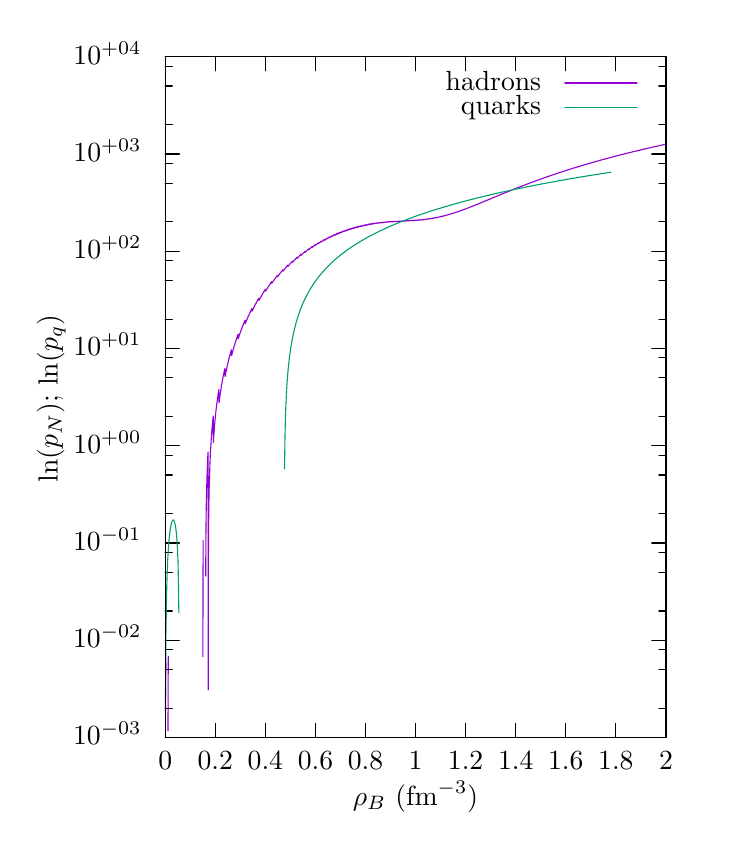
\begin{tikzpicture}[gnuplot]
%% generated with GNUPLOT 5.0p4 (Lua 5.2; terminal rev. 99, script rev. 100)
%% Thu Sep 29 16:33:17 2016
\path (0.000,0.000) rectangle (8.600,10.000);
\gpcolor{color=gp lt color border}
\gpsetlinetype{gp lt border}
\gpsetdashtype{gp dt solid}
\gpsetlinewidth{1.00}
\draw[gp path] (1.688,0.985)--(1.868,0.985);
\draw[gp path] (8.047,0.985)--(7.867,0.985);
\node[gp node right] at (1.504,0.985) {$10^{-03}$};
\draw[gp path] (1.688,1.357)--(1.778,1.357);
\draw[gp path] (8.047,1.357)--(7.957,1.357);
\draw[gp path] (1.688,1.848)--(1.778,1.848);
\draw[gp path] (8.047,1.848)--(7.957,1.848);
\draw[gp path] (1.688,2.100)--(1.778,2.100);
\draw[gp path] (8.047,2.100)--(7.957,2.100);
\draw[gp path] (1.688,2.220)--(1.868,2.220);
\draw[gp path] (8.047,2.220)--(7.867,2.220);
\node[gp node right] at (1.504,2.220) {$10^{-02}$};
\draw[gp path] (1.688,2.592)--(1.778,2.592);
\draw[gp path] (8.047,2.592)--(7.957,2.592);
\draw[gp path] (1.688,3.083)--(1.778,3.083);
\draw[gp path] (8.047,3.083)--(7.957,3.083);
\draw[gp path] (1.688,3.336)--(1.778,3.336);
\draw[gp path] (8.047,3.336)--(7.957,3.336);
\draw[gp path] (1.688,3.455)--(1.868,3.455);
\draw[gp path] (8.047,3.455)--(7.867,3.455);
\node[gp node right] at (1.504,3.455) {$10^{-01}$};
\draw[gp path] (1.688,3.827)--(1.778,3.827);
\draw[gp path] (8.047,3.827)--(7.957,3.827);
\draw[gp path] (1.688,4.319)--(1.778,4.319);
\draw[gp path] (8.047,4.319)--(7.957,4.319);
\draw[gp path] (1.688,4.571)--(1.778,4.571);
\draw[gp path] (8.047,4.571)--(7.957,4.571);
\draw[gp path] (1.688,4.690)--(1.868,4.690);
\draw[gp path] (8.047,4.690)--(7.867,4.690);
\node[gp node right] at (1.504,4.690) {$10^{+00}$};
\draw[gp path] (1.688,5.062)--(1.778,5.062);
\draw[gp path] (8.047,5.062)--(7.957,5.062);
\draw[gp path] (1.688,5.554)--(1.778,5.554);
\draw[gp path] (8.047,5.554)--(7.957,5.554);
\draw[gp path] (1.688,5.806)--(1.778,5.806);
\draw[gp path] (8.047,5.806)--(7.957,5.806);
\draw[gp path] (1.688,5.926)--(1.868,5.926);
\draw[gp path] (8.047,5.926)--(7.867,5.926);
\node[gp node right] at (1.504,5.926) {$10^{+01}$};
\draw[gp path] (1.688,6.297)--(1.778,6.297);
\draw[gp path] (8.047,6.297)--(7.957,6.297);
\draw[gp path] (1.688,6.789)--(1.778,6.789);
\draw[gp path] (8.047,6.789)--(7.957,6.789);
\draw[gp path] (1.688,7.041)--(1.778,7.041);
\draw[gp path] (8.047,7.041)--(7.957,7.041);
\draw[gp path] (1.688,7.161)--(1.868,7.161);
\draw[gp path] (8.047,7.161)--(7.867,7.161);
\node[gp node right] at (1.504,7.161) {$10^{+02}$};
\draw[gp path] (1.688,7.533)--(1.778,7.533);
\draw[gp path] (8.047,7.533)--(7.957,7.533);
\draw[gp path] (1.688,8.024)--(1.778,8.024);
\draw[gp path] (8.047,8.024)--(7.957,8.024);
\draw[gp path] (1.688,8.276)--(1.778,8.276);
\draw[gp path] (8.047,8.276)--(7.957,8.276);
\draw[gp path] (1.688,8.396)--(1.868,8.396);
\draw[gp path] (8.047,8.396)--(7.867,8.396);
\node[gp node right] at (1.504,8.396) {$10^{+03}$};
\draw[gp path] (1.688,8.768)--(1.778,8.768);
\draw[gp path] (8.047,8.768)--(7.957,8.768);
\draw[gp path] (1.688,9.259)--(1.778,9.259);
\draw[gp path] (8.047,9.259)--(7.957,9.259);
\draw[gp path] (1.688,9.511)--(1.778,9.511);
\draw[gp path] (8.047,9.511)--(7.957,9.511);
\draw[gp path] (1.688,9.631)--(1.868,9.631);
\draw[gp path] (8.047,9.631)--(7.867,9.631);
\node[gp node right] at (1.504,9.631) {$10^{+04}$};
\draw[gp path] (1.688,0.985)--(1.688,1.165);
\draw[gp path] (1.688,9.631)--(1.688,9.451);
\node[gp node center] at (1.688,0.677) {$0$};
\draw[gp path] (2.324,0.985)--(2.324,1.165);
\draw[gp path] (2.324,9.631)--(2.324,9.451);
\node[gp node center] at (2.324,0.677) {$0.2$};
\draw[gp path] (2.960,0.985)--(2.960,1.165);
\draw[gp path] (2.960,9.631)--(2.960,9.451);
\node[gp node center] at (2.960,0.677) {$0.4$};
\draw[gp path] (3.596,0.985)--(3.596,1.165);
\draw[gp path] (3.596,9.631)--(3.596,9.451);
\node[gp node center] at (3.596,0.677) {$0.6$};
\draw[gp path] (4.232,0.985)--(4.232,1.165);
\draw[gp path] (4.232,9.631)--(4.232,9.451);
\node[gp node center] at (4.232,0.677) {$0.8$};
\draw[gp path] (4.868,0.985)--(4.868,1.165);
\draw[gp path] (4.868,9.631)--(4.868,9.451);
\node[gp node center] at (4.868,0.677) {$1$};
\draw[gp path] (5.503,0.985)--(5.503,1.165);
\draw[gp path] (5.503,9.631)--(5.503,9.451);
\node[gp node center] at (5.503,0.677) {$1.2$};
\draw[gp path] (6.139,0.985)--(6.139,1.165);
\draw[gp path] (6.139,9.631)--(6.139,9.451);
\node[gp node center] at (6.139,0.677) {$1.4$};
\draw[gp path] (6.775,0.985)--(6.775,1.165);
\draw[gp path] (6.775,9.631)--(6.775,9.451);
\node[gp node center] at (6.775,0.677) {$1.6$};
\draw[gp path] (7.411,0.985)--(7.411,1.165);
\draw[gp path] (7.411,9.631)--(7.411,9.451);
\node[gp node center] at (7.411,0.677) {$1.8$};
\draw[gp path] (8.047,0.985)--(8.047,1.165);
\draw[gp path] (8.047,9.631)--(8.047,9.451);
\node[gp node center] at (8.047,0.677) {$2$};
\draw[gp path] (1.688,9.631)--(1.688,0.985)--(8.047,0.985)--(8.047,9.631)--cycle;
\node[gp node center,rotate=-270] at (0.246,5.308) {$\ln(p_N)$; $\ln(p_q)$};
\node[gp node center] at (4.867,0.215) {$\rho_B$ ($\rm{fm}^{-3}$)};
\node[gp node right] at (6.579,9.297) {hadrons};
\gpcolor{rgb color={0.580,0.000,0.827}}
\draw[gp path] (6.763,9.297)--(7.679,9.297);
\draw[gp path] (1.691,1.321)--(1.693,1.688)--(1.695,1.937);
\draw[gp path] (1.723,1.071)--(1.725,1.709)--(1.727,2.015);
\draw[gp path] (2.166,2.012)--(2.168,3.145)--(2.170,3.486);
\draw[gp path] (2.202,3.036)--(2.204,3.458)--(2.206,3.693)--(2.208,3.858)--(2.210,3.984)%
  --(2.213,4.087)--(2.215,4.175)--(2.217,4.250)--(2.219,4.317)--(2.221,4.377)--(2.223,4.432)%
  --(2.225,4.481)--(2.227,4.527)--(2.229,4.570)--(2.232,4.610)--(2.234,1.589)--(2.236,3.204)%
  --(2.238,3.565)--(2.240,3.780)--(2.242,3.935)--(2.244,4.055)--(2.246,4.155)--(2.249,4.239)%
  --(2.251,4.312)--(2.253,4.378)--(2.255,4.436)--(2.257,4.489)--(2.259,4.538)--(2.261,4.583)%
  --(2.263,4.625)--(2.266,4.664)--(2.268,4.701)--(2.270,4.736)--(2.272,4.769)--(2.274,4.800)%
  --(2.276,4.830)--(2.278,4.858)--(2.280,4.885)--(2.282,4.911)--(2.285,4.936)--(2.287,4.960)%
  --(2.289,4.984)--(2.291,5.006)--(2.293,5.028)--(2.295,5.049)--(2.297,5.069)--(2.299,4.732)%
  --(2.302,4.767)--(2.304,4.800)--(2.306,4.832)--(2.308,4.862)--(2.310,4.891)--(2.312,4.918)%
  --(2.314,4.944)--(2.316,4.970)--(2.318,4.994)--(2.321,5.017)--(2.323,5.040)--(2.325,5.062)%
  --(2.327,5.083)--(2.329,5.103)--(2.331,5.123)--(2.333,5.143)--(2.335,5.161)--(2.338,5.179)%
  --(2.340,5.197)--(2.342,5.215)--(2.344,5.231)--(2.346,5.248)--(2.348,5.264)--(2.350,5.280)%
  --(2.352,5.295)--(2.355,5.310)--(2.357,5.325)--(2.359,5.339)--(2.361,5.353)--(2.363,5.367)%
  --(2.365,5.381)--(2.367,5.394)--(2.369,5.407)--(2.371,5.236)--(2.374,5.253)--(2.376,5.270)%
  --(2.378,5.286)--(2.380,5.302)--(2.382,5.318)--(2.384,5.333)--(2.386,5.348)--(2.388,5.363)%
  --(2.391,5.377)--(2.393,5.391)--(2.395,5.405)--(2.397,5.418)--(2.399,5.432)--(2.401,5.445)%
  --(2.403,5.457)--(2.405,5.470)--(2.408,5.482)--(2.410,5.494)--(2.412,5.506)--(2.414,5.518)%
  --(2.416,5.530)--(2.418,5.541)--(2.420,5.552)--(2.422,5.563)--(2.424,5.574)--(2.427,5.585)%
  --(2.429,5.595)--(2.431,5.606)--(2.433,5.616)--(2.435,5.626)--(2.437,5.636)--(2.439,5.646)%
  --(2.441,5.656)--(2.444,5.666)--(2.446,5.675)--(2.448,5.568)--(2.450,5.579)--(2.452,5.590)%
  --(2.454,5.601)--(2.456,5.612)--(2.458,5.622)--(2.460,5.633)--(2.463,5.643)--(2.465,5.653)%
  --(2.467,5.663)--(2.469,5.673)--(2.471,5.683)--(2.473,5.693)--(2.475,5.702)--(2.477,5.712)%
  --(2.480,5.721)--(2.482,5.730)--(2.484,5.739)--(2.486,5.748)--(2.488,5.757)--(2.490,5.766)%
  --(2.492,5.775)--(2.494,5.783)--(2.497,5.792)--(2.499,5.800)--(2.501,5.808)--(2.503,5.817)%
  --(2.505,5.825)--(2.507,5.833)--(2.509,5.841)--(2.511,5.849)--(2.513,5.857)--(2.516,5.864)%
  --(2.518,5.872)--(2.520,5.880)--(2.522,5.887)--(2.524,5.895)--(2.526,5.902)--(2.528,5.909)%
  --(2.530,5.836)--(2.533,5.844)--(2.535,5.852)--(2.537,5.860)--(2.539,5.868)--(2.541,5.876)%
  --(2.543,5.884)--(2.545,5.892)--(2.547,5.899)--(2.550,5.907)--(2.552,5.914)--(2.554,5.922)%
  --(2.556,5.929)--(2.558,5.936)--(2.560,5.944)--(2.562,5.951)--(2.564,5.958)--(2.566,5.965)%
  --(2.569,5.972)--(2.571,5.979)--(2.573,5.986)--(2.575,5.993)--(2.577,5.999)--(2.579,6.006)%
  --(2.581,6.013)--(2.583,6.019)--(2.586,6.026)--(2.588,6.032)--(2.590,6.039)--(2.592,6.045)%
  --(2.594,6.052)--(2.596,6.058)--(2.598,6.064)--(2.600,6.070)--(2.602,6.077)--(2.605,6.083)%
  --(2.607,6.089)--(2.609,6.095)--(2.611,6.101)--(2.613,6.107)--(2.615,6.053)--(2.617,6.059)%
  --(2.619,6.066)--(2.622,6.072)--(2.624,6.078)--(2.626,6.085)--(2.628,6.091)--(2.630,6.097)%
  --(2.632,6.103)--(2.634,6.109)--(2.636,6.115)--(2.639,6.121)--(2.641,6.127)--(2.643,6.133)%
  --(2.645,6.139)--(2.647,6.145)--(2.649,6.151)--(2.651,6.156)--(2.653,6.162)--(2.655,6.168)%
  --(2.658,6.173)--(2.660,6.179)--(2.662,6.184)--(2.664,6.190)--(2.666,6.196)--(2.668,6.201)%
  --(2.670,6.206)--(2.672,6.212)--(2.675,6.217)--(2.677,6.223)--(2.679,6.228)--(2.681,6.233)%
  --(2.683,6.238)--(2.685,6.244)--(2.687,6.249)--(2.689,6.254)--(2.691,6.259)--(2.694,6.264)%
  --(2.696,6.269)--(2.698,6.274)--(2.700,6.279)--(2.702,6.284)--(2.704,6.243)--(2.706,6.248)%
  --(2.708,6.253)--(2.711,6.259)--(2.713,6.264)--(2.715,6.269)--(2.717,6.274)--(2.719,6.279)%
  --(2.721,6.284)--(2.723,6.289)--(2.725,6.294)--(2.728,6.299)--(2.730,6.304)--(2.732,6.309)%
  --(2.734,6.314)--(2.736,6.319)--(2.738,6.324)--(2.740,6.328)--(2.742,6.333)--(2.744,6.338)%
  --(2.747,6.343)--(2.749,6.347)--(2.751,6.352)--(2.753,6.357)--(2.755,6.361)--(2.757,6.366)%
  --(2.759,6.371)--(2.761,6.375)--(2.764,6.380)--(2.766,6.384)--(2.768,6.389)--(2.770,6.393)%
  --(2.772,6.398)--(2.774,6.402)--(2.776,6.407)--(2.778,6.411)--(2.781,6.416)--(2.783,6.420)%
  --(2.785,6.424)--(2.787,6.429)--(2.789,6.433)--(2.791,6.399)--(2.793,6.404)--(2.795,6.408)%
  --(2.797,6.413)--(2.800,6.417)--(2.802,6.422)--(2.804,6.426)--(2.806,6.431)--(2.808,6.435)%
  --(2.810,6.439)--(2.812,6.444)--(2.814,6.448)--(2.817,6.452)--(2.819,6.456)--(2.821,6.461)%
  --(2.823,6.465)--(2.825,6.469)--(2.827,6.473)--(2.829,6.477)--(2.831,6.481)--(2.833,6.486)%
  --(2.836,6.490)--(2.838,6.494)--(2.840,6.498)--(2.842,6.502)--(2.844,6.506)--(2.846,6.510)%
  --(2.848,6.514)--(2.850,6.518)--(2.853,6.522)--(2.855,6.526)--(2.857,6.530)--(2.859,6.534)%
  --(2.861,6.537)--(2.863,6.541)--(2.865,6.545)--(2.867,6.549)--(2.870,6.553)--(2.872,6.557)%
  --(2.874,6.561)--(2.876,6.564)--(2.878,6.537)--(2.880,6.541)--(2.882,6.544)--(2.884,6.548)%
  --(2.886,6.552)--(2.889,6.556)--(2.891,6.560)--(2.893,6.564)--(2.895,6.568)--(2.897,6.571)%
  --(2.899,6.575)--(2.901,6.579)--(2.903,6.583)--(2.906,6.586)--(2.908,6.590)--(2.910,6.594)%
  --(2.912,6.598)--(2.914,6.601)--(2.916,6.605)--(2.918,6.609)--(2.920,6.612)--(2.923,6.616)%
  --(2.925,6.619)--(2.927,6.623)--(2.929,6.627)--(2.931,6.630)--(2.933,6.634)--(2.935,6.637)%
  --(2.937,6.641)--(2.939,6.644)--(2.942,6.648)--(2.944,6.651)--(2.946,6.655)--(2.948,6.658)%
  --(2.950,6.662)--(2.952,6.665)--(2.954,6.669)--(2.956,6.672)--(2.959,6.675)--(2.961,6.679)%
  --(2.963,6.655)--(2.965,6.659)--(2.967,6.662)--(2.969,6.666)--(2.971,6.669)--(2.973,6.673)%
  --(2.975,6.676)--(2.978,6.680)--(2.980,6.683)--(2.982,6.686)--(2.984,6.690)--(2.986,6.693)%
  --(2.988,6.696)--(2.990,6.700)--(2.992,6.703)--(2.995,6.706)--(2.997,6.710)--(2.999,6.713)%
  --(3.001,6.716)--(3.003,6.720)--(3.005,6.723)--(3.007,6.726)--(3.009,6.729)--(3.012,6.733)%
  --(3.014,6.736)--(3.016,6.739)--(3.018,6.742)--(3.020,6.746)--(3.022,6.749)--(3.024,6.752)%
  --(3.026,6.755)--(3.028,6.758)--(3.031,6.761)--(3.033,6.765)--(3.035,6.768)--(3.037,6.771)%
  --(3.039,6.774)--(3.041,6.753)--(3.043,6.756)--(3.045,6.759)--(3.048,6.763)--(3.050,6.766)%
  --(3.052,6.769)--(3.054,6.772)--(3.056,6.775)--(3.058,6.778)--(3.060,6.781)--(3.062,6.785)%
  --(3.064,6.788)--(3.067,6.791)--(3.069,6.794)--(3.071,6.797)--(3.073,6.800)--(3.075,6.803)%
  --(3.077,6.806)--(3.079,6.809)--(3.081,6.812)--(3.084,6.815)--(3.086,6.818)--(3.088,6.821)%
  --(3.090,6.824)--(3.092,6.827)--(3.094,6.830)--(3.096,6.833)--(3.098,6.836)--(3.101,6.839)%
  --(3.103,6.841)--(3.105,6.844)--(3.107,6.847)--(3.109,6.850)--(3.111,6.853)--(3.113,6.856)%
  --(3.115,6.837)--(3.117,6.840)--(3.120,6.843)--(3.122,6.846)--(3.124,6.849)--(3.126,6.852)%
  --(3.128,6.855)--(3.130,6.858)--(3.132,6.861)--(3.134,6.863)--(3.137,6.866)--(3.139,6.869)%
  --(3.141,6.872)--(3.143,6.875)--(3.145,6.878)--(3.147,6.880)--(3.149,6.883)--(3.151,6.886)%
  --(3.154,6.889)--(3.156,6.892)--(3.158,6.894)--(3.160,6.897)--(3.162,6.900)--(3.164,6.903)%
  --(3.166,6.906)--(3.168,6.908)--(3.170,6.911)--(3.173,6.914)--(3.175,6.916)--(3.177,6.919)%
  --(3.179,6.922)--(3.181,6.925)--(3.183,6.908)--(3.185,6.910)--(3.187,6.913)--(3.190,6.916)%
  --(3.192,6.918)--(3.194,6.921)--(3.196,6.924)--(3.198,6.927)--(3.200,6.929)--(3.202,6.932)%
  --(3.204,6.935)--(3.206,6.937)--(3.209,6.940)--(3.211,6.943)--(3.213,6.945)--(3.215,6.948)%
  --(3.217,6.951)--(3.219,6.953)--(3.221,6.956)--(3.223,6.958)--(3.226,6.961)--(3.228,6.964)%
  --(3.230,6.966)--(3.232,6.969)--(3.234,6.971)--(3.236,6.974)--(3.238,6.977)--(3.240,6.979)%
  --(3.243,6.982)--(3.245,6.984)--(3.247,6.968)--(3.249,6.971)--(3.251,6.974)--(3.253,6.976)%
  --(3.255,6.979)--(3.257,6.981)--(3.259,6.984)--(3.262,6.987)--(3.264,6.989)--(3.266,6.992)%
  --(3.268,6.994)--(3.270,6.997)--(3.272,6.999)--(3.274,7.002)--(3.276,7.004)--(3.279,7.007)%
  --(3.281,7.009)--(3.283,7.012)--(3.285,7.014)--(3.287,7.017)--(3.289,7.019)--(3.291,7.022)%
  --(3.293,7.024)--(3.295,7.026)--(3.298,7.029)--(3.300,7.031)--(3.302,7.034)--(3.304,7.036)%
  --(3.306,7.021)--(3.308,7.024)--(3.310,7.026)--(3.312,7.029)--(3.315,7.031)--(3.317,7.034)%
  --(3.319,7.036)--(3.321,7.039)--(3.323,7.041)--(3.325,7.043)--(3.327,7.046)--(3.329,7.048)%
  --(3.332,7.051)--(3.334,7.053)--(3.336,7.055)--(3.338,7.058)--(3.340,7.060)--(3.342,7.063)%
  --(3.344,7.065)--(3.346,7.067)--(3.348,7.070)--(3.351,7.072)--(3.353,7.074)--(3.355,7.077)%
  --(3.357,7.079)--(3.359,7.081)--(3.361,7.084)--(3.363,7.070)--(3.365,7.072)--(3.368,7.074)%
  --(3.370,7.077)--(3.372,7.079)--(3.374,7.081)--(3.376,7.084)--(3.378,7.086)--(3.380,7.088)%
  --(3.382,7.091)--(3.385,7.093)--(3.387,7.095)--(3.389,7.098)--(3.391,7.100)--(3.393,7.102)%
  --(3.395,7.105)--(3.397,7.107)--(3.399,7.109)--(3.401,7.111)--(3.404,7.114)--(3.406,7.116)%
  --(3.408,7.118)--(3.410,7.120)--(3.412,7.123)--(3.414,7.109)--(3.416,7.112)--(3.418,7.114)%
  --(3.421,7.116)--(3.423,7.118)--(3.425,7.121)--(3.427,7.123)--(3.429,7.125)--(3.431,7.127)%
  --(3.433,7.129)--(3.435,7.132)--(3.437,7.134)--(3.440,7.136)--(3.442,7.138)--(3.444,7.141)%
  --(3.446,7.143)--(3.448,7.145)--(3.450,7.147)--(3.452,7.149)--(3.454,7.151)--(3.457,7.154)%
  --(3.459,7.156)--(3.461,7.158)--(3.463,7.145)--(3.465,7.147)--(3.467,7.150)--(3.469,7.152)%
  --(3.471,7.154)--(3.474,7.156)--(3.476,7.158)--(3.478,7.160)--(3.480,7.163)--(3.482,7.165)%
  --(3.484,7.167)--(3.486,7.169)--(3.488,7.171)--(3.490,7.173)--(3.493,7.175)--(3.495,7.178)%
  --(3.497,7.180)--(3.499,7.182)--(3.501,7.184)--(3.503,7.186)--(3.505,7.188)--(3.507,7.190)%
  --(3.510,7.178)--(3.512,7.180)--(3.514,7.182)--(3.516,7.184)--(3.518,7.186)--(3.520,7.189)%
  --(3.522,7.191)--(3.524,7.193)--(3.527,7.195)--(3.529,7.197)--(3.531,7.199)--(3.533,7.201)%
  --(3.535,7.203)--(3.537,7.205)--(3.539,7.207)--(3.541,7.209)--(3.543,7.211)--(3.546,7.213)%
  --(3.548,7.215)--(3.550,7.218)--(3.552,7.220)--(3.554,7.208)--(3.556,7.210)--(3.558,7.212)%
  --(3.560,7.214)--(3.563,7.216)--(3.565,7.218)--(3.567,7.220)--(3.569,7.222)--(3.571,7.224)%
  --(3.573,7.226)--(3.575,7.228)--(3.577,7.230)--(3.579,7.232)--(3.582,7.234)--(3.584,7.236)%
  --(3.586,7.238)--(3.588,7.240)--(3.590,7.242)--(3.592,7.244)--(3.594,7.233)--(3.596,7.235)%
  --(3.599,7.237)--(3.601,7.239)--(3.603,7.241)--(3.605,7.243)--(3.607,7.245)--(3.609,7.247)%
  --(3.611,7.249)--(3.613,7.251)--(3.616,7.253)--(3.618,7.255)--(3.620,7.257)--(3.622,7.258)%
  --(3.624,7.260)--(3.626,7.262)--(3.628,7.264)--(3.630,7.266)--(3.632,7.268)--(3.635,7.257)%
  --(3.637,7.259)--(3.639,7.261)--(3.641,7.263)--(3.643,7.265)--(3.645,7.267)--(3.647,7.269)%
  --(3.649,7.271)--(3.652,7.273)--(3.654,7.275)--(3.656,7.276)--(3.658,7.278)--(3.660,7.280)%
  --(3.662,7.282)--(3.664,7.284)--(3.666,7.286)--(3.668,7.288)--(3.671,7.290)--(3.673,7.279)%
  --(3.675,7.281)--(3.677,7.283)--(3.679,7.285)--(3.681,7.287)--(3.683,7.288)--(3.685,7.290)%
  --(3.688,7.292)--(3.690,7.294)--(3.692,7.296)--(3.694,7.298)--(3.696,7.300)--(3.698,7.302)%
  --(3.700,7.304)--(3.702,7.305)--(3.705,7.307)--(3.707,7.309)--(3.709,7.298)--(3.711,7.300)%
  --(3.713,7.302)--(3.715,7.304)--(3.717,7.306)--(3.719,7.308)--(3.721,7.310)--(3.724,7.312)%
  --(3.726,7.313)--(3.728,7.315)--(3.730,7.317)--(3.732,7.319)--(3.734,7.321)--(3.736,7.323)%
  --(3.738,7.324)--(3.741,7.326)--(3.743,7.316)--(3.745,7.318)--(3.747,7.319)--(3.749,7.321)%
  --(3.751,7.323)--(3.753,7.325)--(3.755,7.327)--(3.758,7.329)--(3.760,7.330)--(3.762,7.332)%
  --(3.764,7.334)--(3.766,7.336)--(3.768,7.338)--(3.770,7.339)--(3.772,7.341)--(3.774,7.343)%
  --(3.777,7.333)--(3.779,7.335)--(3.781,7.336)--(3.783,7.338)--(3.785,7.340)--(3.787,7.342)%
  --(3.789,7.344)--(3.791,7.345)--(3.794,7.347)--(3.796,7.349)--(3.798,7.351)--(3.800,7.353)%
  --(3.802,7.354)--(3.804,7.356)--(3.806,7.358)--(3.808,7.348)--(3.810,7.349)--(3.813,7.351)%
  --(3.815,7.353)--(3.817,7.355)--(3.819,7.357)--(3.821,7.358)--(3.823,7.360)--(3.825,7.362)%
  --(3.827,7.364)--(3.830,7.365)--(3.832,7.367)--(3.834,7.369)--(3.836,7.371)--(3.838,7.372)%
  --(3.840,7.362)--(3.842,7.364)--(3.844,7.366)--(3.847,7.368)--(3.849,7.369)--(3.851,7.371)%
  --(3.853,7.373)--(3.855,7.375)--(3.857,7.376)--(3.859,7.378)--(3.861,7.380)--(3.863,7.382)%
  --(3.866,7.383)--(3.868,7.385)--(3.870,7.375)--(3.872,7.377)--(3.874,7.378)--(3.876,7.380)%
  --(3.878,7.382)--(3.880,7.384)--(3.883,7.385)--(3.885,7.387)--(3.887,7.389)--(3.889,7.391)%
  --(3.891,7.392)--(3.893,7.394)--(3.895,7.396)--(3.897,7.397)--(3.900,7.387)--(3.902,7.389)%
  --(3.904,7.391)--(3.906,7.393)--(3.908,7.394)--(3.910,7.396)--(3.912,7.398)--(3.914,7.399)%
  --(3.916,7.401)--(3.919,7.403)--(3.921,7.405)--(3.923,7.406)--(3.925,7.408)--(3.927,7.398)%
  --(3.929,7.400)--(3.931,7.402)--(3.933,7.403)--(3.936,7.405)--(3.938,7.407)--(3.940,7.408)%
  --(3.942,7.410)--(3.944,7.412)--(3.946,7.413)--(3.948,7.415)--(3.950,7.417)--(3.952,7.418)%
  --(3.955,7.409)--(3.957,7.410)--(3.959,7.412)--(3.961,7.414)--(3.963,7.415)--(3.965,7.417)%
  --(3.967,7.419)--(3.969,7.420)--(3.972,7.422)--(3.974,7.424)--(3.976,7.425)--(3.978,7.427)%
  --(3.980,7.417)--(3.982,7.419)--(3.984,7.421)--(3.986,7.422)--(3.989,7.424)--(3.991,7.426)%
  --(3.993,7.427)--(3.995,7.429)--(3.997,7.430)--(3.999,7.432)--(4.001,7.434)--(4.003,7.435)%
  --(4.005,7.437)--(4.008,7.427)--(4.010,7.429)--(4.012,7.431)--(4.014,7.432)--(4.016,7.434)%
  --(4.018,7.436)--(4.020,7.437)--(4.022,7.439)--(4.025,7.441)--(4.027,7.442)--(4.029,7.444)%
  --(4.031,7.445)--(4.033,7.436)--(4.035,7.438)--(4.037,7.439)--(4.039,7.441)--(4.041,7.442)%
  --(4.044,7.444)--(4.046,7.446)--(4.048,7.447)--(4.050,7.449)--(4.052,7.450)--(4.054,7.452)%
  --(4.056,7.443)--(4.058,7.444)--(4.061,7.446)--(4.063,7.447)--(4.065,7.449)--(4.067,7.451)%
  --(4.069,7.452)--(4.071,7.454)--(4.073,7.455)--(4.075,7.457)--(4.078,7.459)--(4.080,7.460)%
  --(4.082,7.451)--(4.084,7.452)--(4.086,7.454)--(4.088,7.456)--(4.090,7.457)--(4.092,7.459)%
  --(4.094,7.460)--(4.097,7.462)--(4.099,7.464)--(4.101,7.465)--(4.103,7.467)--(4.105,7.457)%
  --(4.107,7.459)--(4.109,7.461)--(4.111,7.462)--(4.114,7.464)--(4.116,7.465)--(4.118,7.467)%
  --(4.120,7.468)--(4.122,7.470)--(4.124,7.472)--(4.126,7.473)--(4.128,7.464)--(4.131,7.465)%
  --(4.133,7.467)--(4.135,7.469)--(4.137,7.470)--(4.139,7.472)--(4.141,7.473)--(4.143,7.475)%
  --(4.145,7.476)--(4.147,7.478)--(4.150,7.469)--(4.152,7.470)--(4.154,7.472)--(4.156,7.473)%
  --(4.158,7.475)--(4.160,7.476)--(4.162,7.478)--(4.164,7.480)--(4.167,7.481)--(4.169,7.483)%
  --(4.171,7.484)--(4.173,7.475)--(4.175,7.476)--(4.177,7.478)--(4.179,7.480)--(4.181,7.481)%
  --(4.183,7.483)--(4.186,7.484)--(4.188,7.486)--(4.190,7.487)--(4.192,7.489)--(4.194,7.480)%
  --(4.196,7.481)--(4.198,7.483)--(4.200,7.484)--(4.203,7.486)--(4.205,7.487)--(4.207,7.489)%
  --(4.209,7.490)--(4.211,7.492)--(4.213,7.493)--(4.215,7.484)--(4.217,7.486)--(4.220,7.487)%
  --(4.222,7.489)--(4.224,7.490)--(4.226,7.492)--(4.228,7.493)--(4.230,7.495)--(4.232,7.496)%
  --(4.234,7.498)--(4.236,7.489)--(4.239,7.490)--(4.241,7.492)--(4.243,7.493)--(4.245,7.495)%
  --(4.247,7.496)--(4.249,7.498)--(4.251,7.499)--(4.253,7.501)--(4.256,7.502)--(4.258,7.493)%
  --(4.260,7.495)--(4.262,7.496)--(4.264,7.498)--(4.266,7.499)--(4.268,7.501)--(4.270,7.502)%
  --(4.273,7.504)--(4.275,7.505)--(4.277,7.507)--(4.279,7.498)--(4.281,7.499)--(4.283,7.501)%
  --(4.285,7.502)--(4.287,7.504)--(4.289,7.505)--(4.292,7.507)--(4.294,7.508)--(4.296,7.510)%
  --(4.298,7.501)--(4.300,7.502)--(4.302,7.504)--(4.304,7.505)--(4.306,7.507)--(4.309,7.508)%
  --(4.311,7.510)--(4.313,7.511)--(4.315,7.512)--(4.317,7.514)--(4.319,7.505)--(4.321,7.506)%
  --(4.323,7.508)--(4.325,7.509)--(4.328,7.511)--(4.330,7.512)--(4.332,7.514)--(4.334,7.515)%
  --(4.336,7.517)--(4.338,7.510)--(4.340,7.512)--(4.342,7.513)--(4.345,7.515)--(4.347,7.511)%
  --(4.349,7.512)--(4.351,7.514)--(4.353,7.515)--(4.355,7.517)--(4.357,7.513)--(4.359,7.515)%
  --(4.362,7.516)--(4.364,7.517)--(4.366,7.514)--(4.368,7.515)--(4.370,7.517)--(4.372,7.518)%
  --(4.374,7.520)--(4.376,7.516)--(4.378,7.517)--(4.381,7.519)--(4.383,7.520)--(4.385,7.516)%
  --(4.387,7.518)--(4.389,7.519)--(4.391,7.521)--(4.393,7.522)--(4.395,7.518)--(4.398,7.520)%
  --(4.400,7.521)--(4.402,7.523)--(4.404,7.519)--(4.406,7.520)--(4.408,7.522)--(4.410,7.523)%
  --(4.412,7.525)--(4.414,7.521)--(4.417,7.523)--(4.419,7.524)--(4.421,7.525)--(4.423,7.522)%
  --(4.425,7.523)--(4.427,7.525)--(4.429,7.526)--(4.431,7.522)--(4.434,7.524)--(4.436,7.525)%
  --(4.438,7.527)--(4.440,7.528)--(4.442,7.524)--(4.444,7.526)--(4.446,7.527)--(4.448,7.529)%
  --(4.451,7.525)--(4.453,7.526)--(4.455,7.528)--(4.457,7.529)--(4.459,7.525)--(4.461,7.527)%
  --(4.463,7.528)--(4.465,7.530)--(4.467,7.526)--(4.470,7.527)--(4.472,7.529)--(4.474,7.530)%
  --(4.476,7.532)--(4.478,7.528)--(4.480,7.529)--(4.482,7.531)--(4.484,7.532)--(4.487,7.528)%
  --(4.489,7.530)--(4.491,7.531)--(4.493,7.533)--(4.495,7.529)--(4.497,7.530)--(4.499,7.532)%
  --(4.501,7.533)--(4.504,7.529)--(4.506,7.531)--(4.508,7.532)--(4.510,7.534)--(4.512,7.530)%
  --(4.514,7.531)--(4.516,7.533)--(4.518,7.534)--(4.520,7.536)--(4.523,7.532)--(4.525,7.533)%
  --(4.527,7.535)--(4.529,7.536)--(4.531,7.532)--(4.533,7.534)--(4.535,7.535)--(4.537,7.537)%
  --(4.540,7.533)--(4.542,7.534)--(4.544,7.536)--(4.546,7.537)--(4.548,7.533)--(4.550,7.535)%
  --(4.552,7.536)--(4.554,7.538)--(4.556,7.534)--(4.559,7.535)--(4.561,7.537)--(4.563,7.538)%
  --(4.565,7.534)--(4.567,7.536)--(4.569,7.537)--(4.571,7.539)--(4.573,7.535)--(4.576,7.536)%
  --(4.578,7.538)--(4.580,7.539)--(4.582,7.535)--(4.584,7.537)--(4.586,7.538)--(4.588,7.540)%
  --(4.590,7.536)--(4.593,7.537)--(4.595,7.539)--(4.597,7.540)--(4.599,7.536)--(4.601,7.538)%
  --(4.603,7.539)--(4.605,7.540)--(4.607,7.537)--(4.609,7.538)--(4.612,7.540)--(4.614,7.541)%
  --(4.616,7.537)--(4.618,7.539)--(4.620,7.540)--(4.622,7.541)--(4.624,7.538)--(4.626,7.539)%
  --(4.629,7.540)--(4.631,7.542)--(4.633,7.538)--(4.635,7.539)--(4.637,7.541)--(4.639,7.542)%
  --(4.641,7.539)--(4.643,7.540)--(4.646,7.541)--(4.648,7.543)--(4.650,7.539)--(4.652,7.540)%
  --(4.654,7.542)--(4.656,7.543)--(4.658,7.539)--(4.660,7.541)--(4.662,7.542)--(4.665,7.544)%
  --(4.667,7.540)--(4.669,7.541)--(4.671,7.543)--(4.673,7.544)--(4.675,7.540)--(4.677,7.542)%
  --(4.679,7.543)--(4.682,7.545)--(4.684,7.541)--(4.686,7.542)--(4.688,7.544)--(4.690,7.545)%
  --(4.692,7.541)--(4.694,7.543)--(4.696,7.544)--(4.698,7.545)--(4.701,7.542)--(4.703,7.543)%
  --(4.705,7.545)--(4.707,7.546)--(4.709,7.542)--(4.711,7.544)--(4.713,7.545)--(4.715,7.546)%
  --(4.718,7.543)--(4.720,7.544)--(4.722,7.545)--(4.724,7.547)--(4.726,7.543)--(4.728,7.545)%
  --(4.730,7.546)--(4.732,7.547)--(4.735,7.544)--(4.737,7.545)--(4.739,7.546)--(4.741,7.548)%
  --(4.743,7.544)--(4.745,7.546)--(4.747,7.547)--(4.749,7.548)--(4.751,7.545)--(4.754,7.546)%
  --(4.756,7.547)--(4.758,7.549)--(4.760,7.545)--(4.762,7.546)--(4.764,7.548)--(4.766,7.549)%
  --(4.768,7.546)--(4.771,7.547)--(4.773,7.548)--(4.775,7.550)--(4.777,7.546)--(4.779,7.547)%
  --(4.781,7.549)--(4.783,7.550)--(4.785,7.547)--(4.787,7.548)--(4.790,7.549)--(4.792,7.551)%
  --(4.794,7.547)--(4.796,7.548)--(4.798,7.550)--(4.800,7.551)--(4.802,7.548)--(4.804,7.549)%
  --(4.807,7.550)--(4.809,7.552)--(4.811,7.548)--(4.813,7.549)--(4.815,7.551)--(4.817,7.552)%
  --(4.819,7.549)--(4.821,7.550)--(4.824,7.551)--(4.826,7.553)--(4.828,7.549)--(4.830,7.551)%
  --(4.832,7.552)--(4.834,7.553)--(4.836,7.550)--(4.838,7.551)--(4.840,7.552)--(4.843,7.554)%
  --(4.845,7.550)--(4.847,7.552)--(4.849,7.553)--(4.851,7.554)--(4.853,7.551)--(4.855,7.552)%
  --(4.857,7.553)--(4.860,7.555)--(4.862,7.551)--(4.864,7.553)--(4.866,7.554)--(4.868,7.555)%
  --(4.870,7.552)--(4.872,7.553)--(4.874,7.555)--(4.877,7.556)--(4.879,7.553)--(4.881,7.554)%
  --(4.883,7.555)--(4.885,7.557)--(4.887,7.553)--(4.889,7.554)--(4.891,7.556)--(4.893,7.557)%
  --(4.896,7.554)--(4.898,7.555)--(4.900,7.556)--(4.902,7.558)--(4.904,7.554)--(4.906,7.556)%
  --(4.908,7.557)--(4.910,7.558)--(4.913,7.555)--(4.915,7.556)--(4.917,7.558)--(4.919,7.559)%
  --(4.921,7.556)--(4.923,7.557)--(4.925,7.558)--(4.927,7.560)--(4.929,7.556)--(4.932,7.558)%
  --(4.934,7.559)--(4.936,7.560)--(4.938,7.557)--(4.940,7.558)--(4.942,7.560)--(4.944,7.561)%
  --(4.946,7.562)--(4.949,7.559)--(4.951,7.560)--(4.953,7.562)--(4.955,7.563)--(4.957,7.560)%
  --(4.959,7.561)--(4.961,7.562)--(4.963,7.564)--(4.966,7.560)--(4.968,7.562)--(4.970,7.563)%
  --(4.972,7.564)--(4.974,7.561)--(4.976,7.563)--(4.978,7.564)--(4.980,7.565)--(4.982,7.562)%
  --(4.985,7.563)--(4.987,7.565)--(4.989,7.566)--(4.991,7.567)--(4.993,7.564)--(4.995,7.565)%
  --(4.997,7.567)--(4.999,7.568)--(5.002,7.565)--(5.004,7.566)--(5.006,7.568)--(5.008,7.569)%
  --(5.010,7.566)--(5.012,7.567)--(5.014,7.568)--(5.016,7.570)--(5.019,7.567)--(5.021,7.568)%
  --(5.023,7.569)--(5.025,7.571)--(5.027,7.572)--(5.029,7.569)--(5.031,7.570)--(5.033,7.571)%
  --(5.035,7.573)--(5.038,7.570)--(5.040,7.571)--(5.042,7.572)--(5.044,7.574)--(5.046,7.571)%
  --(5.048,7.572)--(5.050,7.573)--(5.052,7.575)--(5.055,7.576)--(5.057,7.573)--(5.059,7.574)%
  --(5.061,7.575)--(5.063,7.577)--(5.065,7.574)--(5.067,7.575)--(5.069,7.576)--(5.071,7.578)%
  --(5.074,7.579)--(5.076,7.576)--(5.078,7.577)--(5.080,7.579)--(5.082,7.580)--(5.084,7.577)%
  --(5.086,7.578)--(5.088,7.580)--(5.091,7.581)--(5.093,7.582)--(5.095,7.579)--(5.097,7.581)%
  --(5.099,7.582)--(5.101,7.583)--(5.103,7.581)--(5.105,7.582)--(5.108,7.583)--(5.110,7.584)%
  --(5.112,7.586)--(5.114,7.583)--(5.116,7.584)--(5.118,7.585)--(5.120,7.587)--(5.122,7.584)%
  --(5.124,7.585)--(5.127,7.587)--(5.129,7.588)--(5.131,7.589)--(5.133,7.586)--(5.135,7.588)%
  --(5.137,7.589)--(5.139,7.590)--(5.141,7.592)--(5.144,7.589)--(5.146,7.590)--(5.148,7.591)%
  --(5.150,7.593)--(5.152,7.590)--(5.154,7.591)--(5.156,7.593)--(5.158,7.594)--(5.160,7.595)%
  --(5.163,7.593)--(5.165,7.594)--(5.167,7.595)--(5.169,7.596)--(5.171,7.598)--(5.173,7.595)%
  --(5.175,7.596)--(5.177,7.598)--(5.180,7.599)--(5.182,7.600)--(5.184,7.598)--(5.186,7.599)%
  --(5.188,7.600)--(5.190,7.602)--(5.192,7.603)--(5.194,7.600)--(5.197,7.602)--(5.199,7.603)%
  --(5.201,7.604)--(5.203,7.602)--(5.205,7.603)--(5.207,7.604)--(5.209,7.606)--(5.211,7.607)%
  --(5.213,7.604)--(5.216,7.606)--(5.218,7.607)--(5.220,7.608)--(5.222,7.609)--(5.224,7.607)%
  --(5.226,7.608)--(5.228,7.610)--(5.230,7.611)--(5.233,7.612)--(5.235,7.611)--(5.237,7.612)%
  --(5.239,7.613)--(5.241,7.613)--(5.243,7.614)--(5.245,7.615)--(5.247,7.615)--(5.250,7.616)%
  --(5.252,7.615)--(5.254,7.617)--(5.256,7.618)--(5.258,7.617)--(5.260,7.619)--(5.262,7.618)%
  --(5.264,7.619)--(5.266,7.621)--(5.269,7.620)--(5.271,7.621)--(5.273,7.623)--(5.275,7.622)%
  --(5.277,7.624)--(5.279,7.623)--(5.281,7.624)--(5.283,7.626)--(5.286,7.625)--(5.288,7.626)%
  --(5.290,7.628)--(5.292,7.627)--(5.294,7.628)--(5.296,7.628)--(5.298,7.629)--(5.300,7.630)%
  --(5.302,7.630)--(5.305,7.631)--(5.307,7.633)--(5.309,7.632)--(5.311,7.633)--(5.313,7.633)%
  --(5.315,7.634)--(5.317,7.635)--(5.319,7.635)--(5.322,7.636)--(5.324,7.638)--(5.326,7.637)%
  --(5.328,7.638)--(5.330,7.640)--(5.332,7.639)--(5.334,7.640)--(5.336,7.640)--(5.339,7.641)%
  --(5.341,7.643)--(5.343,7.642)--(5.345,7.644)--(5.347,7.645)--(5.349,7.644)--(5.351,7.646)%
  --(5.353,7.647)--(5.355,7.647)--(5.358,7.648)--(5.360,7.649)--(5.362,7.649)--(5.364,7.650)%
  --(5.366,7.651)--(5.368,7.651)--(5.370,7.652)--(5.372,7.653)--(5.375,7.653)--(5.377,7.654)%
  --(5.379,7.654)--(5.381,7.655)--(5.383,7.656)--(5.385,7.656)--(5.387,7.657)--(5.389,7.658)%
  --(5.392,7.658)--(5.394,7.659)--(5.396,7.661)--(5.398,7.660)--(5.400,7.662)--(5.402,7.663)%
  --(5.404,7.663)--(5.406,7.664)--(5.408,7.665)--(5.411,7.665)--(5.413,7.666)--(5.415,7.667)%
  --(5.417,7.667)--(5.419,7.668)--(5.421,7.669)--(5.423,7.669)--(5.425,7.670)--(5.428,7.672)%
  --(5.430,7.673)--(5.432,7.673)--(5.434,7.674)--(5.436,7.675)--(5.438,7.675)--(5.440,7.676)%
  --(5.442,7.677)--(5.444,7.677)--(5.447,7.678)--(5.449,7.679)--(5.451,7.679)--(5.453,7.680)%
  --(5.455,7.682)--(5.457,7.682)--(5.459,7.683)--(5.461,7.684)--(5.464,7.684)--(5.466,7.685)%
  --(5.468,7.686)--(5.470,7.687)--(5.472,7.687)--(5.474,7.688)--(5.476,7.689)--(5.478,7.689)%
  --(5.481,7.691)--(5.483,7.692)--(5.485,7.692)--(5.487,7.693)--(5.489,7.694)--(5.491,7.694)%
  --(5.493,7.695)--(5.495,7.696)--(5.497,7.697)--(5.500,7.697)--(5.502,7.699)--(5.504,7.700)%
  --(5.506,7.700)--(5.508,7.701)--(5.510,7.702)--(5.512,7.702)--(5.514,7.703)--(5.517,7.704)%
  --(5.519,7.705)--(5.521,7.705)--(5.523,7.707)--(5.525,7.708)--(5.527,7.708)--(5.529,7.709)%
  --(5.531,7.710)--(5.533,7.711)--(5.536,7.711)--(5.538,7.712)--(5.540,7.713)--(5.542,7.713)%
  --(5.544,7.715)--(5.546,7.716)--(5.548,7.717)--(5.550,7.717)--(5.553,7.718)--(5.555,7.719)%
  --(5.557,7.719)--(5.559,7.720)--(5.561,7.721)--(5.563,7.723)--(5.565,7.723)--(5.567,7.724)%
  --(5.570,7.725)--(5.572,7.725)--(5.574,7.726)--(5.576,7.727)--(5.578,7.728)--(5.580,7.728)%
  --(5.582,7.730)--(5.584,7.731)--(5.586,7.732)--(5.589,7.732)--(5.591,7.733)--(5.593,7.734)%
  --(5.595,7.734)--(5.597,7.735)--(5.599,7.736)--(5.601,7.737)--(5.603,7.738)--(5.606,7.739)%
  --(5.608,7.740)--(5.610,7.741)--(5.612,7.741)--(5.614,7.742)--(5.616,7.743)--(5.618,7.744)%
  --(5.620,7.745)--(5.623,7.746)--(5.625,7.747)--(5.627,7.747)--(5.629,7.748)--(5.631,7.749)%
  --(5.633,7.750)--(5.635,7.750)--(5.637,7.752)--(5.639,7.753)--(5.642,7.754)--(5.644,7.754)%
  --(5.646,7.755)--(5.648,7.756)--(5.650,7.757)--(5.652,7.757)--(5.654,7.758)--(5.656,7.759)%
  --(5.659,7.761)--(5.661,7.761)--(5.663,7.762)--(5.665,7.763)--(5.667,7.764)--(5.669,7.764)%
  --(5.671,7.765)--(5.673,7.766)--(5.675,7.767)--(5.678,7.768)--(5.680,7.769)--(5.682,7.770)%
  --(5.684,7.771)--(5.686,7.771)--(5.688,7.772)--(5.690,7.773)--(5.692,7.774)--(5.695,7.775)%
  --(5.697,7.776)--(5.699,7.777)--(5.701,7.778)--(5.703,7.778)--(5.705,7.779)--(5.707,7.780)%
  --(5.709,7.781)--(5.712,7.782)--(5.714,7.783)--(5.716,7.784)--(5.718,7.785)--(5.720,7.786)%
  --(5.722,7.786)--(5.724,7.787)--(5.726,7.788)--(5.728,7.789)--(5.731,7.790)--(5.733,7.791)%
  --(5.735,7.792)--(5.737,7.793)--(5.739,7.794)--(5.741,7.794)--(5.743,7.795)--(5.745,7.796)%
  --(5.748,7.797)--(5.750,7.798)--(5.752,7.799)--(5.754,7.800)--(5.756,7.801)--(5.758,7.801)%
  --(5.760,7.802)--(5.762,7.803)--(5.764,7.804)--(5.767,7.805)--(5.769,7.806)--(5.771,7.806)%
  --(5.773,7.807)--(5.775,7.808)--(5.777,7.809)--(5.779,7.810)--(5.781,7.811)--(5.784,7.812)%
  --(5.786,7.813)--(5.788,7.813)--(5.790,7.814)--(5.792,7.815)--(5.794,7.816)--(5.796,7.817)%
  --(5.798,7.818)--(5.801,7.819)--(5.803,7.820)--(5.805,7.821)--(5.807,7.821)--(5.809,7.822)%
  --(5.811,7.823)--(5.813,7.824)--(5.815,7.825)--(5.817,7.826)--(5.820,7.827)--(5.822,7.828)%
  --(5.824,7.829)--(5.826,7.830)--(5.828,7.830)--(5.830,7.831)--(5.832,7.832)--(5.834,7.833)%
  --(5.837,7.834)--(5.839,7.835)--(5.841,7.836)--(5.843,7.837)--(5.845,7.837)--(5.847,7.838)%
  --(5.849,7.839)--(5.851,7.840)--(5.854,7.841)--(5.856,7.842)--(5.858,7.843)--(5.860,7.843)%
  --(5.862,7.844)--(5.864,7.845)--(5.866,7.846)--(5.868,7.847)--(5.870,7.848)--(5.873,7.849)%
  --(5.875,7.850)--(5.877,7.851)--(5.879,7.851)--(5.881,7.852)--(5.883,7.853)--(5.885,7.854)%
  --(5.887,7.855)--(5.890,7.856)--(5.892,7.857)--(5.894,7.858)--(5.896,7.859)--(5.898,7.859)%
  --(5.900,7.860)--(5.902,7.861)--(5.904,7.862)--(5.906,7.863)--(5.909,7.864)--(5.911,7.865)%
  --(5.913,7.865)--(5.915,7.866)--(5.917,7.867)--(5.919,7.868)--(5.921,7.869)--(5.923,7.870)%
  --(5.926,7.871)--(5.928,7.872)--(5.930,7.873)--(5.932,7.873)--(5.934,7.874)--(5.936,7.875)%
  --(5.938,7.876)--(5.940,7.877)--(5.943,7.878)--(5.945,7.879)--(5.947,7.879)--(5.949,7.880)%
  --(5.951,7.881)--(5.953,7.882)--(5.955,7.883)--(5.957,7.884)--(5.959,7.885)--(5.962,7.886)%
  --(5.964,7.886)--(5.966,7.887)--(5.968,7.888)--(5.970,7.889)--(5.972,7.890)--(5.974,7.891)%
  --(5.976,7.892)--(5.979,7.893)--(5.981,7.893)--(5.983,7.894)--(5.985,7.895)--(5.987,7.896)%
  --(5.989,7.897)--(5.991,7.898)--(5.993,7.899)--(5.996,7.899)--(5.998,7.900)--(6.000,7.901)%
  --(6.002,7.902)--(6.004,7.903)--(6.006,7.904)--(6.008,7.905)--(6.010,7.906)--(6.012,7.906)%
  --(6.015,7.907)--(6.017,7.908)--(6.019,7.909)--(6.021,7.910)--(6.023,7.911)--(6.025,7.912)%
  --(6.027,7.912)--(6.029,7.913)--(6.032,7.914)--(6.034,7.915)--(6.036,7.916)--(6.038,7.917)%
  --(6.040,7.918)--(6.042,7.918)--(6.044,7.919)--(6.046,7.920)--(6.048,7.921)--(6.051,7.922)%
  --(6.053,7.923)--(6.055,7.924)--(6.057,7.924)--(6.059,7.925)--(6.061,7.926)--(6.063,7.927)%
  --(6.065,7.928)--(6.068,7.929)--(6.070,7.930)--(6.072,7.930)--(6.074,7.931)--(6.076,7.932)%
  --(6.078,7.933)--(6.080,7.934)--(6.082,7.935)--(6.085,7.936)--(6.087,7.936)--(6.089,7.937)%
  --(6.091,7.938)--(6.093,7.939)--(6.095,7.940)--(6.097,7.941)--(6.099,7.941)--(6.101,7.942)%
  --(6.104,7.943)--(6.106,7.944)--(6.108,7.945)--(6.110,7.946)--(6.112,7.947)--(6.114,7.947)%
  --(6.116,7.948)--(6.118,7.949)--(6.121,7.950)--(6.123,7.951)--(6.125,7.952)--(6.127,7.952)%
  --(6.129,7.953)--(6.131,7.954)--(6.133,7.955)--(6.135,7.956)--(6.137,7.957)--(6.140,7.958)%
  --(6.142,7.958)--(6.144,7.959)--(6.146,7.960)--(6.148,7.961)--(6.150,7.962)--(6.152,7.962)%
  --(6.154,7.963)--(6.157,7.964)--(6.159,7.965)--(6.161,7.966)--(6.163,7.967)--(6.165,7.967)%
  --(6.167,7.968)--(6.169,7.969)--(6.171,7.970)--(6.174,7.971)--(6.176,7.972)--(6.178,7.973)%
  --(6.180,7.973)--(6.182,7.974)--(6.184,7.975)--(6.186,7.976)--(6.188,7.977)--(6.190,7.977)%
  --(6.193,7.978)--(6.195,7.979)--(6.197,7.980)--(6.199,7.981)--(6.201,7.982)--(6.203,7.982)%
  --(6.205,7.983)--(6.207,7.984)--(6.210,7.985)--(6.212,7.986)--(6.214,7.987)--(6.216,7.987)%
  --(6.218,7.988)--(6.220,7.989)--(6.222,7.990)--(6.224,7.991)--(6.227,7.991)--(6.229,7.992)%
  --(6.231,7.993)--(6.233,7.994)--(6.235,7.995)--(6.237,7.996)--(6.239,7.996)--(6.241,7.997)%
  --(6.243,7.998)--(6.246,7.999)--(6.248,8.000)--(6.250,8.000)--(6.252,8.001)--(6.254,8.002)%
  --(6.256,8.003)--(6.258,8.004)--(6.260,8.005)--(6.263,8.005)--(6.265,8.006)--(6.267,8.007)%
  --(6.269,8.008)--(6.271,8.009)--(6.273,8.009)--(6.275,8.010)--(6.277,8.011)--(6.279,8.012)%
  --(6.282,8.012)--(6.284,8.013)--(6.286,8.014)--(6.288,8.015)--(6.290,8.016)--(6.292,8.017)%
  --(6.294,8.017)--(6.296,8.018)--(6.299,8.019)--(6.301,8.020)--(6.303,8.021)--(6.305,8.021)%
  --(6.307,8.022)--(6.309,8.023)--(6.311,8.024)--(6.313,8.025)--(6.316,8.025)--(6.318,8.026)%
  --(6.320,8.027)--(6.322,8.028)--(6.324,8.028)--(6.326,8.029)--(6.328,8.030)--(6.330,8.031)%
  --(6.332,8.032)--(6.335,8.033)--(6.337,8.033)--(6.339,8.034)--(6.341,8.035)--(6.343,8.036)%
  --(6.345,8.036)--(6.347,8.037)--(6.349,8.038)--(6.352,8.039)--(6.354,8.040)--(6.356,8.040)%
  --(6.358,8.041)--(6.360,8.042)--(6.362,8.043)--(6.364,8.044)--(6.366,8.044)--(6.369,8.045)%
  --(6.371,8.046)--(6.373,8.047)--(6.375,8.047)--(6.377,8.048)--(6.379,8.049)--(6.381,8.050)%
  --(6.383,8.051)--(6.385,8.051)--(6.388,8.052)--(6.390,8.053)--(6.392,8.054)--(6.394,8.054)%
  --(6.396,8.055)--(6.398,8.056)--(6.400,8.057)--(6.402,8.057)--(6.405,8.058)--(6.407,8.059)%
  --(6.409,8.060)--(6.411,8.061)--(6.413,8.061)--(6.415,8.062)--(6.417,8.063)--(6.419,8.064)%
  --(6.421,8.064)--(6.424,8.065)--(6.426,8.066)--(6.428,8.067)--(6.430,8.068)--(6.432,8.068)%
  --(6.434,8.069)--(6.436,8.070)--(6.438,8.071)--(6.441,8.071)--(6.443,8.072)--(6.445,8.073)%
  --(6.447,8.074)--(6.449,8.074)--(6.451,8.075)--(6.453,8.076)--(6.455,8.077)--(6.458,8.077)%
  --(6.460,8.078)--(6.462,8.079)--(6.464,8.080)--(6.466,8.081)--(6.468,8.081)--(6.470,8.082)%
  --(6.472,8.083)--(6.474,8.084)--(6.477,8.084)--(6.479,8.085)--(6.481,8.086)--(6.483,8.086)%
  --(6.485,8.087)--(6.487,8.088)--(6.489,8.089)--(6.491,8.089)--(6.494,8.090)--(6.496,8.091)%
  --(6.498,8.092)--(6.500,8.092)--(6.502,8.093)--(6.504,8.094)--(6.506,8.095)--(6.508,8.096)%
  --(6.510,8.096)--(6.513,8.097)--(6.515,8.098)--(6.517,8.099)--(6.519,8.099)--(6.521,8.100)%
  --(6.523,8.101)--(6.525,8.102)--(6.527,8.102)--(6.530,8.103)--(6.532,8.104)--(6.534,8.104)%
  --(6.536,8.105)--(6.538,8.106)--(6.540,8.107)--(6.542,8.107)--(6.544,8.108)--(6.547,8.109)%
  --(6.549,8.110)--(6.551,8.110)--(6.553,8.111)--(6.555,8.112)--(6.557,8.113)--(6.559,8.113)%
  --(6.561,8.114)--(6.563,8.115)--(6.566,8.115)--(6.568,8.116)--(6.570,8.117)--(6.572,8.118)%
  --(6.574,8.118)--(6.576,8.119)--(6.578,8.120)--(6.580,8.121)--(6.583,8.121)--(6.585,8.122)%
  --(6.587,8.123)--(6.589,8.124)--(6.591,8.124)--(6.593,8.125)--(6.595,8.126)--(6.597,8.126)%
  --(6.600,8.127)--(6.602,8.128)--(6.604,8.129)--(6.606,8.129)--(6.608,8.130)--(6.610,8.131)%
  --(6.612,8.132)--(6.614,8.132)--(6.616,8.133)--(6.619,8.134)--(6.621,8.134)--(6.623,8.135)%
  --(6.625,8.136)--(6.627,8.136)--(6.629,8.137)--(6.631,8.138)--(6.633,8.139)--(6.636,8.139)%
  --(6.638,8.140)--(6.640,8.141)--(6.642,8.141)--(6.644,8.142)--(6.646,8.143)--(6.648,8.144)%
  --(6.650,8.144)--(6.652,8.145)--(6.655,8.146)--(6.657,8.147)--(6.659,8.147)--(6.661,8.148)%
  --(6.663,8.149)--(6.665,8.149)--(6.667,8.150)--(6.669,8.151)--(6.672,8.151)--(6.674,8.152)%
  --(6.676,8.153)--(6.678,8.153)--(6.680,8.154)--(6.682,8.155)--(6.684,8.156)--(6.686,8.156)%
  --(6.689,8.157)--(6.691,8.158)--(6.693,8.159)--(6.695,8.159)--(6.697,8.160)--(6.699,8.160)%
  --(6.701,8.161)--(6.703,8.162)--(6.705,8.163)--(6.708,8.163)--(6.710,8.164)--(6.712,8.165)%
  --(6.714,8.165)--(6.716,8.166)--(6.718,8.167)--(6.720,8.168)--(6.722,8.168)--(6.725,8.169)%
  --(6.727,8.169)--(6.729,8.170)--(6.731,8.171)--(6.733,8.172)--(6.735,8.172)--(6.737,8.173)%
  --(6.739,8.174)--(6.742,8.174)--(6.744,8.175)--(6.746,8.176)--(6.748,8.176)--(6.750,8.177)%
  --(6.752,8.178)--(6.754,8.178)--(6.756,8.179)--(6.758,8.180)--(6.761,8.181)--(6.763,8.181)%
  --(6.765,8.182)--(6.767,8.182)--(6.769,8.183)--(6.771,8.184)--(6.773,8.185)--(6.775,8.185)%
  --(6.778,8.186)--(6.780,8.187)--(6.782,8.187)--(6.784,8.188)--(6.786,8.189)--(6.788,8.189)%
  --(6.790,8.190)--(6.792,8.191)--(6.794,8.192)--(6.797,8.192)--(6.799,8.193)--(6.801,8.193)%
  --(6.803,8.194)--(6.805,8.195)--(6.807,8.195)--(6.809,8.196)--(6.811,8.197)--(6.814,8.197)%
  --(6.816,8.198)--(6.818,8.199)--(6.820,8.199)--(6.822,8.200)--(6.824,8.201)--(6.826,8.202)%
  --(6.828,8.202)--(6.831,8.203)--(6.833,8.203)--(6.835,8.204)--(6.837,8.205)--(6.839,8.206)%
  --(6.841,8.206)--(6.843,8.207)--(6.845,8.207)--(6.847,8.208)--(6.850,8.209)--(6.852,8.210)%
  --(6.854,8.210)--(6.856,8.211)--(6.858,8.211)--(6.860,8.212)--(6.862,8.213)--(6.864,8.214)%
  --(6.867,8.214)--(6.869,8.215)--(6.871,8.215)--(6.873,8.216)--(6.875,8.217)--(6.877,8.218)%
  --(6.879,8.218)--(6.881,8.219)--(6.883,8.219)--(6.886,8.220)--(6.888,8.221)--(6.890,8.221)%
  --(6.892,8.222)--(6.894,8.223)--(6.896,8.223)--(6.898,8.224)--(6.900,8.225)--(6.903,8.225)%
  --(6.905,8.226)--(6.907,8.227)--(6.909,8.227)--(6.911,8.228)--(6.913,8.228)--(6.915,8.229)%
  --(6.917,8.230)--(6.920,8.230)--(6.922,8.231)--(6.924,8.232)--(6.926,8.232)--(6.928,8.233)%
  --(6.930,8.234)--(6.932,8.234)--(6.934,8.235)--(6.936,8.236)--(6.939,8.236)--(6.941,8.237)%
  --(6.943,8.238)--(6.945,8.238)--(6.947,8.239)--(6.949,8.239)--(6.951,8.240)--(6.953,8.241)%
  --(6.956,8.241)--(6.958,8.242)--(6.960,8.243)--(6.962,8.243)--(6.964,8.244)--(6.966,8.245)%
  --(6.968,8.245)--(6.970,8.246)--(6.973,8.246)--(6.975,8.247)--(6.977,8.248)--(6.979,8.248)%
  --(6.981,8.249)--(6.983,8.250)--(6.985,8.250)--(6.987,8.251)--(6.989,8.252)--(6.992,8.252)%
  --(6.994,8.253)--(6.996,8.253)--(6.998,8.254)--(7.000,8.255)--(7.002,8.255)--(7.004,8.256)%
  --(7.006,8.257)--(7.009,8.257)--(7.011,8.258)--(7.013,8.259)--(7.015,8.259)--(7.017,8.260)%
  --(7.019,8.260)--(7.021,8.261)--(7.023,8.262)--(7.025,8.262)--(7.028,8.263)--(7.030,8.264)%
  --(7.032,8.264)--(7.034,8.265)--(7.036,8.265)--(7.038,8.266)--(7.040,8.267)--(7.042,8.267)%
  --(7.045,8.268)--(7.047,8.268)--(7.049,8.269)--(7.051,8.270)--(7.053,8.270)--(7.055,8.271)%
  --(7.057,8.272)--(7.059,8.272)--(7.062,8.273)--(7.064,8.273)--(7.066,8.274)--(7.068,8.275)%
  --(7.070,8.275)--(7.072,8.276)--(7.074,8.276)--(7.076,8.277)--(7.078,8.278)--(7.081,8.278)%
  --(7.083,8.279)--(7.085,8.280)--(7.087,8.280)--(7.089,8.281)--(7.091,8.281)--(7.093,8.282)%
  --(7.095,8.283)--(7.098,8.283)--(7.100,8.284)--(7.102,8.284)--(7.104,8.285)--(7.106,8.286)%
  --(7.108,8.286)--(7.110,8.287)--(7.112,8.287)--(7.115,8.288)--(7.117,8.289)--(7.119,8.289)%
  --(7.121,8.290)--(7.123,8.291)--(7.125,8.291)--(7.127,8.292)--(7.129,8.292)--(7.131,8.293)%
  --(7.134,8.294)--(7.136,8.294)--(7.138,8.295)--(7.140,8.295)--(7.142,8.296)--(7.144,8.297)%
  --(7.146,8.297)--(7.148,8.298)--(7.151,8.298)--(7.153,8.299)--(7.155,8.299)--(7.157,8.300)%
  --(7.159,8.301)--(7.161,8.301)--(7.163,8.302)--(7.165,8.302)--(7.167,8.303)--(7.170,8.304)%
  --(7.172,8.304)--(7.174,8.305)--(7.176,8.306)--(7.178,8.306)--(7.180,8.307)--(7.182,8.307)%
  --(7.184,8.308)--(7.187,8.308)--(7.189,8.309)--(7.191,8.310)--(7.193,8.310)--(7.195,8.311)%
  --(7.197,8.311)--(7.199,8.312)--(7.201,8.313)--(7.204,8.313)--(7.206,8.314)--(7.208,8.314)%
  --(7.210,8.315)--(7.212,8.315)--(7.214,8.316)--(7.216,8.317)--(7.218,8.317)--(7.220,8.318)%
  --(7.223,8.319)--(7.225,8.319)--(7.227,8.320)--(7.229,8.320)--(7.231,8.321)--(7.233,8.321)%
  --(7.235,8.322)--(7.237,8.323)--(7.240,8.323)--(7.242,8.324)--(7.244,8.324)--(7.246,8.325)%
  --(7.248,8.325)--(7.250,8.326)--(7.252,8.327)--(7.254,8.327)--(7.256,8.328)--(7.259,8.328)%
  --(7.261,8.329)--(7.263,8.330)--(7.265,8.330)--(7.267,8.331)--(7.269,8.331)--(7.271,8.332)%
  --(7.273,8.332)--(7.276,8.333)--(7.278,8.334)--(7.280,8.334)--(7.282,8.335)--(7.284,8.335)%
  --(7.286,8.336)--(7.288,8.336)--(7.290,8.337)--(7.293,8.338)--(7.295,8.338)--(7.297,8.339)%
  --(7.299,8.339)--(7.301,8.340)--(7.303,8.340)--(7.305,8.341)--(7.307,8.342)--(7.309,8.342)%
  --(7.312,8.343)--(7.314,8.343)--(7.316,8.344)--(7.318,8.344)--(7.320,8.345)--(7.322,8.346)%
  --(7.324,8.346)--(7.326,8.347)--(7.329,8.347)--(7.331,8.348)--(7.333,8.348)--(7.335,8.349)%
  --(7.337,8.349)--(7.339,8.350)--(7.341,8.351)--(7.343,8.351)--(7.346,8.352)--(7.348,8.352)%
  --(7.350,8.353)--(7.352,8.353)--(7.354,8.354)--(7.356,8.355)--(7.358,8.355)--(7.360,8.356)%
  --(7.362,8.356)--(7.365,8.357)--(7.367,8.357)--(7.369,8.358)--(7.371,8.358)--(7.373,8.359)%
  --(7.375,8.360)--(7.377,8.360)--(7.379,8.361)--(7.382,8.361)--(7.384,8.362)--(7.386,8.362)%
  --(7.388,8.363)--(7.390,8.364)--(7.392,8.364)--(7.394,8.365)--(7.396,8.365)--(7.398,8.366)%
  --(7.401,8.366)--(7.403,8.367)--(7.405,8.367)--(7.407,8.368)--(7.409,8.369)--(7.411,8.369)%
  --(7.413,8.370)--(7.415,8.370)--(7.418,8.371)--(7.420,8.371)--(7.422,8.372)--(7.424,8.372)%
  --(7.426,8.373)--(7.428,8.374)--(7.430,8.374)--(7.432,8.375)--(7.435,8.375)--(7.437,8.376)%
  --(7.439,8.376)--(7.441,8.377)--(7.443,8.377)--(7.445,8.378)--(7.447,8.378)--(7.449,8.379)%
  --(7.451,8.380)--(7.454,8.380)--(7.456,8.381)--(7.458,8.381)--(7.460,8.382)--(7.462,8.382)%
  --(7.464,8.383)--(7.466,8.383)--(7.468,8.384)--(7.471,8.384)--(7.473,8.385)--(7.475,8.386)%
  --(7.477,8.386)--(7.479,8.387)--(7.481,8.387)--(7.483,8.388)--(7.485,8.388)--(7.488,8.389)%
  --(7.490,8.389)--(7.492,8.390)--(7.494,8.390)--(7.496,8.391)--(7.498,8.391)--(7.500,8.392)%
  --(7.502,8.392)--(7.504,8.393)--(7.507,8.393)--(7.509,8.394)--(7.511,8.395)--(7.513,8.395)%
  --(7.515,8.396)--(7.517,8.396)--(7.519,8.397)--(7.521,8.397)--(7.524,8.398)--(7.526,8.398)%
  --(7.528,8.399)--(7.530,8.399)--(7.532,8.400)--(7.534,8.401)--(7.536,8.401)--(7.538,8.402)%
  --(7.540,8.402)--(7.543,8.403)--(7.545,8.403)--(7.547,8.404)--(7.549,8.404)--(7.551,8.405)%
  --(7.553,8.405)--(7.555,8.406)--(7.557,8.406)--(7.560,8.407)--(7.562,8.407)--(7.564,8.408)%
  --(7.566,8.408)--(7.568,8.409)--(7.570,8.410)--(7.572,8.410)--(7.574,8.411)--(7.577,8.411)%
  --(7.579,8.412)--(7.581,8.412)--(7.583,8.413)--(7.585,8.413)--(7.587,8.414)--(7.589,8.414)%
  --(7.591,8.415)--(7.593,8.415)--(7.596,8.416)--(7.598,8.416)--(7.600,8.417)--(7.602,8.417)%
  --(7.604,8.418)--(7.606,8.418)--(7.608,8.419)--(7.610,8.419)--(7.613,8.420)--(7.615,8.420)%
  --(7.617,8.421)--(7.619,8.421)--(7.621,8.422)--(7.623,8.423)--(7.625,8.423)--(7.627,8.424)%
  --(7.629,8.424)--(7.632,8.425)--(7.634,8.425)--(7.636,8.426)--(7.638,8.426)--(7.640,8.427)%
  --(7.642,8.427)--(7.644,8.428)--(7.646,8.428)--(7.649,8.429)--(7.651,8.429)--(7.653,8.430)%
  --(7.655,8.430)--(7.657,8.431)--(7.659,8.431)--(7.661,8.432)--(7.663,8.432)--(7.666,8.433)%
  --(7.668,8.433)--(7.670,8.434)--(7.672,8.434)--(7.674,8.435)--(7.676,8.435)--(7.678,8.436)%
  --(7.680,8.436)--(7.682,8.437)--(7.685,8.437)--(7.687,8.438)--(7.689,8.438)--(7.691,8.439)%
  --(7.693,8.439)--(7.695,8.440)--(7.697,8.440)--(7.699,8.441)--(7.702,8.442)--(7.704,8.442)%
  --(7.706,8.442)--(7.708,8.443)--(7.710,8.443)--(7.712,8.444)--(7.714,8.445)--(7.716,8.445)%
  --(7.719,8.446)--(7.721,8.446)--(7.723,8.446)--(7.725,8.447)--(7.727,8.447)--(7.729,8.448)%
  --(7.731,8.449)--(7.733,8.449)--(7.735,8.450)--(7.738,8.450)--(7.740,8.450)--(7.742,8.451)%
  --(7.744,8.452)--(7.746,8.452)--(7.748,8.453)--(7.750,8.453)--(7.752,8.453)--(7.755,8.454)%
  --(7.757,8.455)--(7.759,8.455)--(7.761,8.456)--(7.763,8.456)--(7.765,8.457)--(7.767,8.457)%
  --(7.769,8.457)--(7.771,8.458)--(7.774,8.459)--(7.776,8.459)--(7.778,8.460)--(7.780,8.460)%
  --(7.782,8.460)--(7.784,8.461)--(7.786,8.462)--(7.788,8.462)--(7.791,8.462)--(7.793,8.463)%
  --(7.795,8.463)--(7.797,8.464)--(7.799,8.465)--(7.801,8.465)--(7.803,8.465)--(7.805,8.466)%
  --(7.808,8.466)--(7.810,8.467)--(7.812,8.467)--(7.814,8.468)--(7.816,8.468)--(7.818,8.469)%
  --(7.820,8.469)--(7.822,8.470)--(7.824,8.470)--(7.827,8.471)--(7.829,8.471)--(7.831,8.472)%
  --(7.833,8.472)--(7.835,8.473)--(7.837,8.473)--(7.839,8.474)--(7.841,8.474)--(7.844,8.475)%
  --(7.846,8.475)--(7.848,8.476)--(7.850,8.476)--(7.852,8.477)--(7.854,8.477)--(7.856,8.478)%
  --(7.858,8.478)--(7.861,8.479)--(7.863,8.479)--(7.865,8.480)--(7.867,8.480)--(7.869,8.481)%
  --(7.871,8.481)--(7.873,8.481)--(7.875,8.482)--(7.877,8.483)--(7.880,8.483)--(7.882,8.483)%
  --(7.884,8.484)--(7.886,8.484)--(7.888,8.485)--(7.890,8.485)--(7.892,8.486)--(7.894,8.486)%
  --(7.897,8.487)--(7.899,8.487)--(7.901,8.488)--(7.903,8.488)--(7.905,8.489)--(7.907,8.489)%
  --(7.909,8.490)--(7.911,8.490)--(7.913,8.491)--(7.916,8.491)--(7.918,8.492)--(7.920,8.492)%
  --(7.922,8.493)--(7.924,8.493)--(7.926,8.494)--(7.928,8.494)--(7.930,8.494)--(7.933,8.495)%
  --(7.935,8.495)--(7.937,8.496)--(7.939,8.496)--(7.941,8.497)--(7.943,8.497)--(7.945,8.498)%
  --(7.947,8.498)--(7.950,8.499)--(7.952,8.499)--(7.954,8.500)--(7.956,8.500)--(7.958,8.501)%
  --(7.960,8.501)--(7.962,8.502)--(7.964,8.502)--(7.966,8.502)--(7.969,8.503)--(7.971,8.504)%
  --(7.973,8.504)--(7.975,8.504)--(7.977,8.505)--(7.979,8.505)--(7.981,8.506)--(7.983,8.506)%
  --(7.986,8.507)--(7.988,8.507)--(7.990,8.508)--(7.992,8.508)--(7.994,8.509)--(7.996,8.509)%
  --(7.998,8.510)--(8.000,8.510)--(8.002,8.510)--(8.005,8.511)--(8.007,8.512)--(8.009,8.512)%
  --(8.011,8.512)--(8.013,8.513)--(8.015,8.513)--(8.017,8.514)--(8.019,8.514)--(8.022,8.515)%
  --(8.024,8.515)--(8.026,8.516)--(8.028,8.516)--(8.030,8.517)--(8.032,8.517)--(8.034,8.517)%
  --(8.036,8.518)--(8.039,8.518)--(8.041,8.519)--(8.043,8.519)--(8.045,8.520)--(8.047,8.520);
\gpcolor{color=gp lt color border}
\node[gp node right] at (6.579,8.989) {quarks};
\gpcolor{rgb color={0.000,0.620,0.451}}
\draw[gp path] (6.763,8.989)--(7.679,8.989);
\draw[gp path] (1.691,1.486)--(1.697,2.308)--(1.703,2.685)--(1.708,2.928)--(1.714,3.099)%
  --(1.719,3.233)--(1.725,3.339)--(1.731,3.422)--(1.736,3.494)--(1.742,3.550)--(1.748,3.600)%
  --(1.753,3.639)--(1.759,3.671)--(1.765,3.700)--(1.770,3.720)--(1.776,3.734)--(1.782,3.743)%
  --(1.787,3.748)--(1.793,3.747)--(1.799,3.742)--(1.804,3.726)--(1.810,3.709)--(1.816,3.680)%
  --(1.821,3.650)--(1.827,3.603)--(1.833,3.543)--(1.838,3.467)--(1.844,3.366)--(1.850,3.227)%
  --(1.855,2.991)--(1.861,2.566);
\draw[gp path] (3.203,4.398)--(3.209,4.812)--(3.214,5.043)--(3.220,5.204)--(3.226,5.328)%
  --(3.231,5.429)--(3.237,5.513)--(3.243,5.587)--(3.248,5.651)--(3.254,5.709)--(3.260,5.761)%
  --(3.265,5.809)--(3.271,5.852)--(3.277,5.893)--(3.282,5.931)--(3.288,5.966)--(3.294,5.999)%
  --(3.299,6.030)--(3.305,6.060)--(3.311,6.088)--(3.316,6.115)--(3.322,6.140)--(3.327,6.164)%
  --(3.333,6.188)--(3.339,6.210)--(3.344,6.231)--(3.350,6.252)--(3.356,6.272)--(3.361,6.291)%
  --(3.367,6.310)--(3.373,6.328)--(3.378,6.345)--(3.384,6.362)--(3.390,6.378)--(3.395,6.394)%
  --(3.401,6.410)--(3.407,6.425)--(3.412,6.440)--(3.418,6.454)--(3.424,6.468)--(3.429,6.481)%
  --(3.435,6.495)--(3.441,6.508)--(3.446,6.520)--(3.452,6.533)--(3.458,6.545)--(3.463,6.557)%
  --(3.469,6.568)--(3.475,6.580)--(3.480,6.591)--(3.486,6.602)--(3.492,6.613)--(3.497,6.623)%
  --(3.503,6.634)--(3.509,6.644)--(3.514,6.654)--(3.520,6.664)--(3.526,6.673)--(3.531,6.683)%
  --(3.537,6.692)--(3.543,6.701)--(3.548,6.710)--(3.554,6.719)--(3.560,6.728)--(3.565,6.736)%
  --(3.571,6.745)--(3.577,6.753)--(3.582,6.762)--(3.588,6.770)--(3.594,6.778)--(3.599,6.786)%
  --(3.605,6.793)--(3.611,6.801)--(3.616,6.809)--(3.622,6.816)--(3.628,6.824)--(3.633,6.831)%
  --(3.639,6.838)--(3.645,6.845)--(3.650,6.852)--(3.656,6.859)--(3.662,6.866)--(3.667,6.873)%
  --(3.673,6.880)--(3.679,6.886)--(3.684,6.893)--(3.690,6.899)--(3.696,6.906)--(3.701,6.912)%
  --(3.707,6.919)--(3.713,6.925)--(3.718,6.931)--(3.724,6.937)--(3.729,6.943)--(3.735,6.949)%
  --(3.741,6.955)--(3.746,6.961)--(3.752,6.966)--(3.758,6.972)--(3.763,6.978)--(3.769,6.983)%
  --(3.775,6.989)--(3.780,6.995)--(3.786,7.000)--(3.792,7.005)--(3.797,7.011)--(3.803,7.016)%
  --(3.809,7.021)--(3.814,7.027)--(3.820,7.032)--(3.826,7.037)--(3.831,7.042)--(3.837,7.047)%
  --(3.843,7.052)--(3.848,7.057)--(3.854,7.062)--(3.860,7.067)--(3.865,7.072)--(3.871,7.076)%
  --(3.877,7.081)--(3.882,7.086)--(3.888,7.091)--(3.894,7.095)--(3.899,7.100)--(3.905,7.104)%
  --(3.911,7.109)--(3.916,7.113)--(3.922,7.118)--(3.928,7.122)--(3.933,7.127)--(3.939,7.131)%
  --(3.945,7.136)--(3.950,7.140)--(3.956,7.144)--(3.962,7.148)--(3.967,7.153)--(3.973,7.157)%
  --(3.979,7.161)--(3.984,7.165)--(3.990,7.169)--(3.996,7.173)--(4.001,7.177)--(4.007,7.181)%
  --(4.013,7.185)--(4.018,7.189)--(4.024,7.193)--(4.030,7.197)--(4.035,7.201)--(4.041,7.205)%
  --(4.047,7.209)--(4.052,7.213)--(4.058,7.216)--(4.064,7.220)--(4.069,7.224)--(4.075,7.228)%
  --(4.081,7.231)--(4.086,7.235)--(4.092,7.239)--(4.098,7.242)--(4.103,7.246)--(4.109,7.249)%
  --(4.115,7.253)--(4.120,7.257)--(4.126,7.260)--(4.131,7.264)--(4.137,7.267)--(4.143,7.271)%
  --(4.148,7.274)--(4.154,7.277)--(4.160,7.281)--(4.165,7.284)--(4.171,7.288)--(4.177,7.291)%
  --(4.182,7.294)--(4.188,7.298)--(4.194,7.301)--(4.199,7.304)--(4.205,7.308)--(4.211,7.311)%
  --(4.216,7.314)--(4.222,7.317)--(4.228,7.320)--(4.233,7.324)--(4.239,7.327)--(4.245,7.330)%
  --(4.250,7.333)--(4.256,7.336)--(4.262,7.339)--(4.267,7.342)--(4.273,7.345)--(4.279,7.348)%
  --(4.284,7.351)--(4.290,7.355)--(4.296,7.358)--(4.301,7.361)--(4.307,7.363)--(4.313,7.366)%
  --(4.318,7.369)--(4.324,7.372)--(4.330,7.375)--(4.335,7.378)--(4.341,7.381)--(4.347,7.384)%
  --(4.352,7.387)--(4.358,7.390)--(4.364,7.393)--(4.369,7.395)--(4.375,7.398)--(4.381,7.401)%
  --(4.386,7.404)--(4.392,7.407)--(4.398,7.409)--(4.403,7.412)--(4.409,7.415)--(4.415,7.418)%
  --(4.420,7.420)--(4.426,7.423)--(4.432,7.426)--(4.437,7.428)--(4.443,7.431)--(4.449,7.434)%
  --(4.454,7.436)--(4.460,7.439)--(4.466,7.442)--(4.471,7.444)--(4.477,7.447)--(4.483,7.449)%
  --(4.488,7.452)--(4.494,7.455)--(4.500,7.457)--(4.505,7.460)--(4.511,7.462)--(4.517,7.465)%
  --(4.522,7.467)--(4.528,7.470)--(4.533,7.472)--(4.539,7.475)--(4.545,7.477)--(4.550,7.480)%
  --(4.556,7.482)--(4.562,7.485)--(4.567,7.487)--(4.573,7.490)--(4.579,7.492)--(4.584,7.494)%
  --(4.590,7.497)--(4.596,7.499)--(4.601,7.502)--(4.607,7.504)--(4.613,7.506)--(4.618,7.509)%
  --(4.624,7.511)--(4.630,7.513)--(4.635,7.516)--(4.641,7.518)--(4.647,7.520)--(4.652,7.523)%
  --(4.658,7.525)--(4.664,7.527)--(4.669,7.529)--(4.675,7.532)--(4.681,7.534)--(4.686,7.536)%
  --(4.692,7.539)--(4.698,7.541)--(4.703,7.543)--(4.709,7.545)--(4.715,7.547)--(4.720,7.550)%
  --(4.726,7.552)--(4.732,7.554)--(4.737,7.556)--(4.743,7.558)--(4.749,7.561)--(4.754,7.563)%
  --(4.760,7.565)--(4.766,7.567)--(4.771,7.569)--(4.777,7.571)--(4.783,7.573)--(4.788,7.576)%
  --(4.794,7.578)--(4.800,7.580)--(4.805,7.582)--(4.811,7.584)--(4.817,7.586)--(4.822,7.588)%
  --(4.828,7.590)--(4.834,7.592)--(4.839,7.594)--(4.845,7.596)--(4.851,7.598)--(4.856,7.601)%
  --(4.862,7.603)--(4.868,7.605)--(4.873,7.607)--(4.879,7.609)--(4.885,7.611)--(4.890,7.613)%
  --(4.896,7.615)--(4.902,7.617)--(4.907,7.619)--(4.913,7.621)--(4.919,7.623)--(4.924,7.624)%
  --(4.930,7.626)--(4.936,7.628)--(4.941,7.630)--(4.947,7.632)--(4.952,7.634)--(4.958,7.636)%
  --(4.964,7.638)--(4.969,7.640)--(4.975,7.642)--(4.981,7.644)--(4.986,7.646)--(4.992,7.648)%
  --(4.998,7.649)--(5.003,7.651)--(5.009,7.653)--(5.015,7.655)--(5.020,7.657)--(5.026,7.659)%
  --(5.032,7.661)--(5.037,7.663)--(5.043,7.664)--(5.049,7.666)--(5.054,7.668)--(5.060,7.670)%
  --(5.066,7.672)--(5.071,7.674)--(5.077,7.675)--(5.083,7.677)--(5.088,7.679)--(5.094,7.681)%
  --(5.100,7.683)--(5.105,7.684)--(5.111,7.686)--(5.117,7.688)--(5.122,7.690)--(5.128,7.691)%
  --(5.134,7.693)--(5.139,7.695)--(5.145,7.697)--(5.151,7.698)--(5.156,7.700)--(5.162,7.702)%
  --(5.168,7.704)--(5.173,7.705)--(5.179,7.707)--(5.185,7.709)--(5.190,7.711)--(5.196,7.712)%
  --(5.202,7.714)--(5.207,7.716)--(5.213,7.717)--(5.219,7.719)--(5.224,7.721)--(5.230,7.722)%
  --(5.236,7.724)--(5.241,7.726)--(5.247,7.728)--(5.253,7.729)--(5.258,7.731)--(5.264,7.733)%
  --(5.270,7.734)--(5.275,7.736)--(5.281,7.737)--(5.287,7.739)--(5.292,7.741)--(5.298,7.742)%
  --(5.304,7.744)--(5.309,7.746)--(5.315,7.747)--(5.321,7.749)--(5.326,7.751)--(5.332,7.752)%
  --(5.338,7.754)--(5.343,7.755)--(5.349,7.757)--(5.354,7.759)--(5.360,7.760)--(5.366,7.762)%
  --(5.371,7.763)--(5.377,7.765)--(5.383,7.766)--(5.388,7.768)--(5.394,7.770)--(5.400,7.771)%
  --(5.405,7.773)--(5.411,7.774)--(5.417,7.776)--(5.422,7.777)--(5.428,7.779)--(5.434,7.780)%
  --(5.439,7.782)--(5.445,7.784)--(5.451,7.785)--(5.456,7.787)--(5.462,7.788)--(5.468,7.790)%
  --(5.473,7.791)--(5.479,7.793)--(5.485,7.794)--(5.490,7.796)--(5.496,7.797)--(5.502,7.799)%
  --(5.507,7.800)--(5.513,7.802)--(5.519,7.803)--(5.524,7.805)--(5.530,7.806)--(5.536,7.808)%
  --(5.541,7.809)--(5.547,7.811)--(5.553,7.812)--(5.558,7.813)--(5.564,7.815)--(5.570,7.816)%
  --(5.575,7.818)--(5.581,7.819)--(5.587,7.821)--(5.592,7.822)--(5.598,7.824)--(5.604,7.825)%
  --(5.609,7.826)--(5.615,7.828)--(5.621,7.829)--(5.626,7.831)--(5.632,7.832)--(5.638,7.834)%
  --(5.643,7.835)--(5.649,7.836)--(5.655,7.838)--(5.660,7.839)--(5.666,7.841)--(5.672,7.842)%
  --(5.677,7.843)--(5.683,7.845)--(5.689,7.846)--(5.694,7.848)--(5.700,7.849)--(5.706,7.850)%
  --(5.711,7.852)--(5.717,7.853)--(5.723,7.855)--(5.728,7.856)--(5.734,7.857)--(5.740,7.859)%
  --(5.745,7.860)--(5.751,7.861)--(5.756,7.863)--(5.762,7.864)--(5.768,7.865)--(5.773,7.867)%
  --(5.779,7.868)--(5.785,7.870)--(5.790,7.871)--(5.796,7.872)--(5.802,7.874)--(5.807,7.875)%
  --(5.813,7.876)--(5.819,7.878)--(5.824,7.879)--(5.830,7.880)--(5.836,7.882)--(5.841,7.883)%
  --(5.847,7.884)--(5.853,7.885)--(5.858,7.887)--(5.864,7.888)--(5.870,7.889)--(5.875,7.891)%
  --(5.881,7.892)--(5.887,7.893)--(5.892,7.895)--(5.898,7.896)--(5.904,7.897)--(5.909,7.898)%
  --(5.915,7.900)--(5.921,7.901)--(5.926,7.902)--(5.932,7.904)--(5.938,7.905)--(5.943,7.906)%
  --(5.949,7.907)--(5.955,7.909)--(5.960,7.910)--(5.966,7.911)--(5.972,7.912)--(5.977,7.914)%
  --(5.983,7.915)--(5.989,7.916)--(5.994,7.917)--(6.000,7.919)--(6.006,7.920)--(6.011,7.921)%
  --(6.017,7.922)--(6.023,7.924)--(6.028,7.925)--(6.034,7.926)--(6.040,7.927)--(6.045,7.929)%
  --(6.051,7.930)--(6.057,7.931)--(6.062,7.932)--(6.068,7.933)--(6.074,7.935)--(6.079,7.936)%
  --(6.085,7.937)--(6.091,7.938)--(6.096,7.940)--(6.102,7.941)--(6.108,7.942)--(6.113,7.943)%
  --(6.119,7.944)--(6.125,7.946)--(6.130,7.947)--(6.136,7.948)--(6.142,7.949)--(6.147,7.950)%
  --(6.153,7.952)--(6.158,7.953)--(6.164,7.954)--(6.170,7.955)--(6.175,7.956)--(6.181,7.957)%
  --(6.187,7.959)--(6.192,7.960)--(6.198,7.961)--(6.204,7.962)--(6.209,7.963)--(6.215,7.964)%
  --(6.221,7.966)--(6.226,7.967)--(6.232,7.968)--(6.238,7.969)--(6.243,7.970)--(6.249,7.971)%
  --(6.255,7.973)--(6.260,7.974)--(6.266,7.975)--(6.272,7.976)--(6.277,7.977)--(6.283,7.978)%
  --(6.289,7.979)--(6.294,7.981)--(6.300,7.982)--(6.306,7.983)--(6.311,7.984)--(6.317,7.985)%
  --(6.323,7.986)--(6.328,7.987)--(6.334,7.988)--(6.340,7.990)--(6.345,7.991)--(6.351,7.992)%
  --(6.357,7.993)--(6.362,7.994)--(6.368,7.995)--(6.374,7.996)--(6.379,7.997)--(6.385,7.998)%
  --(6.391,8.000)--(6.396,8.001)--(6.402,8.002)--(6.408,8.003)--(6.413,8.004)--(6.419,8.005)%
  --(6.425,8.006)--(6.430,8.007)--(6.436,8.008)--(6.442,8.009)--(6.447,8.011)--(6.453,8.012)%
  --(6.459,8.013)--(6.464,8.014)--(6.470,8.015)--(6.476,8.016)--(6.481,8.017)--(6.487,8.018)%
  --(6.493,8.019)--(6.498,8.020)--(6.504,8.021)--(6.510,8.022)--(6.515,8.023)--(6.521,8.025)%
  --(6.527,8.026)--(6.532,8.027)--(6.538,8.028)--(6.544,8.029)--(6.549,8.030)--(6.555,8.031)%
  --(6.560,8.032)--(6.566,8.033)--(6.572,8.034)--(6.577,8.035)--(6.583,8.036)--(6.589,8.037)%
  --(6.594,8.038)--(6.600,8.039)--(6.606,8.040)--(6.611,8.041)--(6.617,8.042)--(6.623,8.043)%
  --(6.628,8.044)--(6.634,8.045)--(6.640,8.046)--(6.645,8.048)--(6.651,8.049)--(6.657,8.050)%
  --(6.662,8.051)--(6.668,8.052)--(6.674,8.053)--(6.679,8.054)--(6.685,8.055)--(6.691,8.056)%
  --(6.696,8.057)--(6.702,8.058)--(6.708,8.059)--(6.713,8.060)--(6.719,8.061)--(6.725,8.062)%
  --(6.730,8.063)--(6.736,8.064)--(6.742,8.065)--(6.747,8.066)--(6.753,8.067)--(6.759,8.068)%
  --(6.764,8.069)--(6.770,8.070)--(6.776,8.071)--(6.781,8.072)--(6.787,8.073)--(6.793,8.074)%
  --(6.798,8.075)--(6.804,8.076)--(6.810,8.077)--(6.815,8.078)--(6.821,8.079)--(6.827,8.080)%
  --(6.832,8.081)--(6.838,8.082)--(6.844,8.083)--(6.849,8.084)--(6.855,8.084)--(6.861,8.085)%
  --(6.866,8.086)--(6.872,8.087)--(6.878,8.088)--(6.883,8.089)--(6.889,8.090)--(6.895,8.091)%
  --(6.900,8.092)--(6.906,8.093)--(6.912,8.094)--(6.917,8.095)--(6.923,8.096)--(6.929,8.097)%
  --(6.934,8.098)--(6.940,8.099)--(6.946,8.100)--(6.951,8.101)--(6.957,8.102)--(6.962,8.103)%
  --(6.968,8.104)--(6.974,8.105)--(6.979,8.106)--(6.985,8.106)--(6.991,8.107)--(6.996,8.108)%
  --(7.002,8.109)--(7.008,8.110)--(7.013,8.111)--(7.019,8.112)--(7.025,8.113)--(7.030,8.114)%
  --(7.036,8.115)--(7.042,8.116)--(7.047,8.117)--(7.053,8.118)--(7.059,8.119)--(7.064,8.120)%
  --(7.070,8.120)--(7.076,8.121)--(7.081,8.122)--(7.087,8.123)--(7.093,8.124)--(7.098,8.125)%
  --(7.104,8.126)--(7.110,8.127)--(7.115,8.128)--(7.121,8.129)--(7.127,8.130)--(7.132,8.131)%
  --(7.138,8.131)--(7.144,8.132)--(7.149,8.133)--(7.155,8.134)--(7.161,8.135)--(7.166,8.136)%
  --(7.172,8.137)--(7.178,8.138)--(7.183,8.139)--(7.189,8.140)--(7.195,8.140)--(7.200,8.141)%
  --(7.206,8.142)--(7.212,8.143)--(7.217,8.144)--(7.223,8.145)--(7.229,8.146)--(7.234,8.147)%
  --(7.240,8.148)--(7.246,8.148)--(7.251,8.149)--(7.257,8.150)--(7.263,8.151)--(7.268,8.152)%
  --(7.274,8.153)--(7.280,8.154)--(7.285,8.155)--(7.291,8.155)--(7.297,8.156)--(7.302,8.157)%
  --(7.308,8.158)--(7.314,8.159)--(7.319,8.160)--(7.325,8.161)--(7.331,8.162)--(7.336,8.162)%
  --(7.342,8.163)--(7.348,8.164);
\gpcolor{color=gp lt color border}
\draw[gp path] (1.688,9.631)--(1.688,0.985)--(8.047,0.985)--(8.047,9.631)--cycle;
%% coordinates of the plot area
\gpdefrectangularnode{gp plot 1}{\pgfpoint{1.688cm}{0.985cm}}{\pgfpoint{8.047cm}{9.631cm}}
\end{tikzpicture}
%% gnuplot variables

	\caption{Buballa\_2-eNJL1m}
\end{figure}
\begin{figure}
	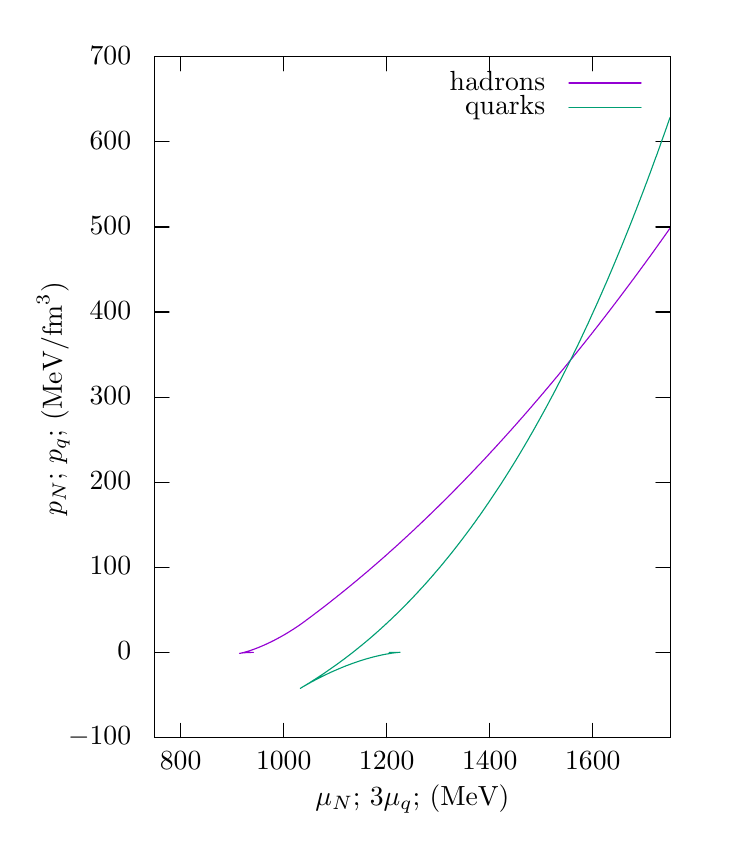
\begin{tikzpicture}[gnuplot]
%% generated with GNUPLOT 5.0p4 (Lua 5.2; terminal rev. 99, script rev. 100)
%% Thu Sep 29 16:33:18 2016
\path (0.000,0.000) rectangle (8.600,10.000);
\gpcolor{color=gp lt color border}
\gpsetlinetype{gp lt border}
\gpsetdashtype{gp dt solid}
\gpsetlinewidth{1.00}
\draw[gp path] (1.504,0.985)--(1.684,0.985);
\draw[gp path] (8.047,0.985)--(7.867,0.985);
\node[gp node right] at (1.320,0.985) {$-100$};
\draw[gp path] (1.504,2.066)--(1.684,2.066);
\draw[gp path] (8.047,2.066)--(7.867,2.066);
\node[gp node right] at (1.320,2.066) {$0$};
\draw[gp path] (1.504,3.147)--(1.684,3.147);
\draw[gp path] (8.047,3.147)--(7.867,3.147);
\node[gp node right] at (1.320,3.147) {$100$};
\draw[gp path] (1.504,4.227)--(1.684,4.227);
\draw[gp path] (8.047,4.227)--(7.867,4.227);
\node[gp node right] at (1.320,4.227) {$200$};
\draw[gp path] (1.504,5.308)--(1.684,5.308);
\draw[gp path] (8.047,5.308)--(7.867,5.308);
\node[gp node right] at (1.320,5.308) {$300$};
\draw[gp path] (1.504,6.389)--(1.684,6.389);
\draw[gp path] (8.047,6.389)--(7.867,6.389);
\node[gp node right] at (1.320,6.389) {$400$};
\draw[gp path] (1.504,7.469)--(1.684,7.469);
\draw[gp path] (8.047,7.469)--(7.867,7.469);
\node[gp node right] at (1.320,7.469) {$500$};
\draw[gp path] (1.504,8.550)--(1.684,8.550);
\draw[gp path] (8.047,8.550)--(7.867,8.550);
\node[gp node right] at (1.320,8.550) {$600$};
\draw[gp path] (1.504,9.631)--(1.684,9.631);
\draw[gp path] (8.047,9.631)--(7.867,9.631);
\node[gp node right] at (1.320,9.631) {$700$};
\draw[gp path] (1.831,0.985)--(1.831,1.165);
\draw[gp path] (1.831,9.631)--(1.831,9.451);
\node[gp node center] at (1.831,0.677) {$800$};
\draw[gp path] (3.140,0.985)--(3.140,1.165);
\draw[gp path] (3.140,9.631)--(3.140,9.451);
\node[gp node center] at (3.140,0.677) {$1000$};
\draw[gp path] (4.448,0.985)--(4.448,1.165);
\draw[gp path] (4.448,9.631)--(4.448,9.451);
\node[gp node center] at (4.448,0.677) {$1200$};
\draw[gp path] (5.757,0.985)--(5.757,1.165);
\draw[gp path] (5.757,9.631)--(5.757,9.451);
\node[gp node center] at (5.757,0.677) {$1400$};
\draw[gp path] (7.066,0.985)--(7.066,1.165);
\draw[gp path] (7.066,9.631)--(7.066,9.451);
\node[gp node center] at (7.066,0.677) {$1600$};
\draw[gp path] (1.504,9.631)--(1.504,0.985)--(8.047,0.985)--(8.047,9.631)--cycle;
\node[gp node center,rotate=-270] at (0.246,5.308) {$p_N$; $p_q$; ($\rm{MeV}/\rm{fm}^3$)};
\node[gp node center] at (4.775,0.215) {$\mu_N$; $3\mu_q$; (MeV)};
\node[gp node right] at (6.579,9.297) {hadrons};
\gpcolor{rgb color={0.580,0.000,0.827}}
\draw[gp path] (6.763,9.297)--(7.679,9.297);
\draw[gp path] (2.725,2.066)--(2.732,2.066)--(2.739,2.066)--(2.745,2.066)--(2.751,2.066)%
  --(2.757,2.066)--(2.725,2.066)--(2.731,2.066)--(2.737,2.066)--(2.743,2.066)--(2.748,2.066)%
  --(2.716,2.065)--(2.721,2.066)--(2.727,2.066)--(2.732,2.066)--(2.738,2.066)--(2.705,2.065)%
  --(2.711,2.065)--(2.716,2.065)--(2.722,2.066)--(2.727,2.066)--(2.733,2.066)--(2.700,2.065)%
  --(2.706,2.065)--(2.711,2.065)--(2.717,2.065)--(2.722,2.066)--(2.690,2.065)--(2.695,2.065)%
  --(2.700,2.065)--(2.706,2.065)--(2.711,2.065)--(2.679,2.064)--(2.684,2.064)--(2.690,2.065)%
  --(2.695,2.065)--(2.700,2.065)--(2.706,2.065)--(2.673,2.064)--(2.679,2.064)--(2.684,2.064)%
  --(2.690,2.065)--(2.695,2.065)--(2.663,2.063)--(2.668,2.063)--(2.674,2.064)--(2.679,2.064)%
  --(2.685,2.064)--(2.690,2.065)--(2.658,2.063)--(2.663,2.063)--(2.669,2.063)--(2.674,2.064)%
  --(2.680,2.064)--(2.648,2.062)--(2.653,2.063)--(2.659,2.063)--(2.664,2.063)--(2.670,2.064)%
  --(2.675,2.064)--(2.643,2.062)--(2.649,2.062)--(2.654,2.063)--(2.660,2.063)--(2.665,2.063)%
  --(2.634,2.061)--(2.639,2.061)--(2.645,2.062)--(2.650,2.062)--(2.656,2.063)--(2.661,2.063)%
  --(2.630,2.061)--(2.635,2.061)--(2.641,2.062)--(2.647,2.062)--(2.652,2.063)--(2.621,2.060)%
  --(2.626,2.060)--(2.632,2.061)--(2.638,2.061)--(2.643,2.062)--(2.649,2.062)--(2.617,2.059)%
  --(2.623,2.060)--(2.629,2.061)--(2.635,2.061)--(2.640,2.062)--(2.609,2.059)--(2.615,2.059)%
  --(2.620,2.060)--(2.626,2.060)--(2.632,2.061)--(2.638,2.061)--(2.606,2.058)--(2.612,2.059)%
  --(2.618,2.059)--(2.624,2.060)--(2.630,2.061)--(2.635,2.061)--(2.604,2.058)--(2.610,2.059)%
  --(2.616,2.059)--(2.622,2.060)--(2.628,2.061)--(2.597,2.057)--(2.602,2.058)--(2.608,2.058)%
  --(2.614,2.059)--(2.620,2.060)--(2.626,2.060)--(2.595,2.057)--(2.601,2.057)--(2.607,2.058)%
  --(2.613,2.059)--(2.619,2.060)--(2.588,2.056)--(2.594,2.056)--(2.600,2.057)--(2.606,2.058)%
  --(2.612,2.059)--(2.618,2.060)--(2.587,2.055)--(2.593,2.056)--(2.599,2.057)--(2.605,2.058)%
  --(2.611,2.059)--(2.618,2.060)--(2.587,2.055)--(2.593,2.056)--(2.599,2.057)--(2.605,2.058)%
  --(2.611,2.059)--(2.617,2.060)--(2.587,2.055)--(2.593,2.056)--(2.599,2.057)--(2.605,2.058)%
  --(2.612,2.059)--(2.581,2.054)--(2.588,2.055)--(2.594,2.056)--(2.600,2.057)--(2.606,2.058)%
  --(2.612,2.059)--(2.582,2.054)--(2.588,2.055)--(2.595,2.056)--(2.601,2.057)--(2.607,2.058)%
  --(2.613,2.059)--(2.583,2.054)--(2.590,2.055)--(2.596,2.057)--(2.602,2.058)--(2.608,2.059)%
  --(2.579,2.054)--(2.585,2.055)--(2.591,2.056)--(2.597,2.057)--(2.604,2.058)--(2.610,2.059)%
  --(2.580,2.054)--(2.587,2.055)--(2.593,2.056)--(2.600,2.057)--(2.606,2.058)--(2.612,2.060)%
  --(2.583,2.054)--(2.589,2.055)--(2.596,2.056)--(2.602,2.058)--(2.608,2.059)--(2.615,2.060)%
  --(2.585,2.054)--(2.592,2.056)--(2.598,2.057)--(2.605,2.058)--(2.611,2.059)--(2.618,2.061)%
  --(2.588,2.055)--(2.595,2.056)--(2.601,2.058)--(2.608,2.059)--(2.614,2.060)--(2.585,2.054)%
  --(2.592,2.056)--(2.598,2.057)--(2.605,2.058)--(2.611,2.060)--(2.618,2.061)--(2.589,2.055)%
  --(2.596,2.056)--(2.602,2.058)--(2.609,2.059)--(2.615,2.061)--(2.622,2.062)--(2.593,2.056)%
  --(2.600,2.057)--(2.606,2.059)--(2.613,2.060)--(2.620,2.062)--(2.626,2.063)--(2.598,2.057)%
  --(2.604,2.058)--(2.611,2.060)--(2.618,2.061)--(2.624,2.063)--(2.596,2.056)--(2.603,2.058)%
  --(2.609,2.059)--(2.616,2.061)--(2.623,2.062)--(2.629,2.064)--(2.601,2.057)--(2.608,2.059)%
  --(2.614,2.060)--(2.621,2.062)--(2.628,2.064)--(2.635,2.065)--(2.607,2.058)--(2.613,2.060)%
  --(2.620,2.062)--(2.627,2.063)--(2.634,2.065)--(2.640,2.067)--(2.612,2.060)--(2.619,2.062)%
  --(2.626,2.063)--(2.633,2.065)--(2.640,2.067)--(2.647,2.068)--(2.619,2.061)--(2.626,2.063)%
  --(2.632,2.065)--(2.639,2.067)--(2.646,2.068)--(2.619,2.061)--(2.625,2.063)--(2.632,2.065)%
  --(2.639,2.067)--(2.646,2.068)--(2.653,2.070)--(2.625,2.063)--(2.632,2.065)--(2.639,2.067)%
  --(2.646,2.069)--(2.653,2.070)--(2.660,2.072)--(2.633,2.065)--(2.640,2.067)--(2.647,2.069)%
  --(2.654,2.071)--(2.661,2.073)--(2.668,2.075)--(2.640,2.067)--(2.648,2.069)--(2.655,2.071)%
  --(2.662,2.073)--(2.669,2.075)--(2.676,2.077)--(2.649,2.069)--(2.656,2.071)--(2.663,2.073)%
  --(2.670,2.075)--(2.677,2.077)--(2.650,2.069)--(2.657,2.071)--(2.664,2.074)--(2.671,2.076)%
  --(2.678,2.078)--(2.685,2.080)--(2.659,2.072)--(2.666,2.074)--(2.673,2.076)--(2.680,2.078)%
  --(2.687,2.080)--(2.694,2.083)--(2.668,2.074)--(2.675,2.077)--(2.682,2.079)--(2.689,2.081)%
  --(2.696,2.083)--(2.703,2.086)--(2.677,2.077)--(2.684,2.080)--(2.691,2.082)--(2.699,2.084)%
  --(2.706,2.086)--(2.679,2.078)--(2.687,2.080)--(2.694,2.083)--(2.701,2.085)--(2.708,2.087)%
  --(2.716,2.090)--(2.689,2.081)--(2.697,2.084)--(2.704,2.086)--(2.711,2.088)--(2.719,2.091)%
  --(2.726,2.093)--(2.700,2.084)--(2.707,2.087)--(2.714,2.089)--(2.722,2.092)--(2.729,2.094)%
  --(2.736,2.097)--(2.710,2.088)--(2.718,2.090)--(2.725,2.093)--(2.732,2.095)--(2.740,2.098)%
  --(2.714,2.089)--(2.722,2.092)--(2.729,2.094)--(2.736,2.097)--(2.744,2.099)--(2.751,2.102)%
  --(2.725,2.093)--(2.733,2.096)--(2.740,2.098)--(2.748,2.101)--(2.755,2.103)--(2.762,2.106)%
  --(2.737,2.097)--(2.745,2.100)--(2.752,2.102)--(2.759,2.105)--(2.767,2.108)--(2.742,2.099)%
  --(2.749,2.101)--(2.757,2.104)--(2.764,2.107)--(2.771,2.109)--(2.779,2.112)--(2.754,2.103)%
  --(2.761,2.106)--(2.769,2.109)--(2.776,2.111)--(2.784,2.114)--(2.767,2.108)--(2.775,2.111)%
  --(2.782,2.113)--(2.773,2.110)--(2.781,2.113)--(2.788,2.116)--(2.780,2.113)--(2.787,2.116)%
  --(2.795,2.118)--(2.786,2.115)--(2.794,2.118)--(2.801,2.121)--(2.793,2.118)--(2.801,2.121)%
  --(2.792,2.117)--(2.800,2.120)--(2.807,2.123)--(2.799,2.120)--(2.806,2.123)--(2.814,2.126)%
  --(2.806,2.123)--(2.813,2.126)--(2.821,2.129)--(2.813,2.125)--(2.820,2.128)--(2.812,2.125)%
  --(2.820,2.128)--(2.827,2.131)--(2.819,2.128)--(2.827,2.131)--(2.834,2.134)--(2.826,2.131)%
  --(2.834,2.134)--(2.841,2.137)--(2.833,2.134)--(2.841,2.137)--(2.833,2.134)--(2.841,2.137)%
  --(2.848,2.140)--(2.840,2.137)--(2.848,2.140)--(2.856,2.143)--(2.848,2.140)--(2.855,2.143)%
  --(2.848,2.140)--(2.855,2.143)--(2.863,2.146)--(2.855,2.143)--(2.863,2.146)--(2.871,2.149)%
  --(2.863,2.146)--(2.870,2.149)--(2.863,2.146)--(2.870,2.149)--(2.878,2.153)--(2.871,2.149)%
  --(2.878,2.153)--(2.886,2.156)--(2.878,2.153)--(2.886,2.156)--(2.879,2.153)--(2.886,2.156)%
  --(2.894,2.160)--(2.887,2.156)--(2.894,2.160)--(2.902,2.163)--(2.895,2.160)--(2.902,2.163)%
  --(2.895,2.160)--(2.903,2.164)--(2.910,2.167)--(2.903,2.164)--(2.911,2.167)--(2.919,2.171)%
  --(2.911,2.168)--(2.919,2.171)--(2.912,2.168)--(2.920,2.171)--(2.927,2.175)--(2.920,2.172)%
  --(2.928,2.175)--(2.921,2.172)--(2.929,2.176)--(2.937,2.179)--(2.929,2.176)--(2.937,2.180)%
  --(2.945,2.183)--(2.938,2.180)--(2.946,2.184)--(2.939,2.180)--(2.947,2.184)--(2.955,2.188)%
  --(2.948,2.184)--(2.955,2.188)--(2.949,2.185)--(2.956,2.189)--(2.964,2.192)--(2.957,2.189)%
  --(2.965,2.193)--(2.959,2.190)--(2.966,2.193)--(2.974,2.197)--(2.968,2.194)--(2.975,2.198)%
  --(2.969,2.195)--(2.977,2.198)--(2.984,2.202)--(2.978,2.199)--(2.986,2.203)--(2.979,2.200)%
  --(2.987,2.204)--(2.995,2.208)--(2.988,2.204)--(2.996,2.208)--(2.990,2.205)--(2.998,2.209)%
  --(3.006,2.213)--(2.999,2.210)--(3.007,2.214)--(3.001,2.210)--(3.009,2.214)--(3.017,2.218)%
  --(3.010,2.215)--(3.018,2.219)--(3.012,2.216)--(3.020,2.220)--(3.014,2.217)--(3.022,2.221)%
  --(3.030,2.225)--(3.024,2.222)--(3.031,2.226)--(3.025,2.223)--(3.033,2.227)--(3.041,2.231)%
  --(3.035,2.228)--(3.043,2.232)--(3.037,2.229)--(3.045,2.233)--(3.039,2.230)--(3.047,2.234)%
  --(3.055,2.239)--(3.049,2.236)--(3.057,2.240)--(3.052,2.237)--(3.060,2.241)--(3.054,2.238)%
  --(3.062,2.242)--(3.070,2.246)--(3.064,2.243)--(3.072,2.248)--(3.066,2.245)--(3.074,2.249)%
  --(3.069,2.246)--(3.077,2.250)--(3.085,2.255)--(3.079,2.252)--(3.087,2.256)--(3.082,2.253)%
  --(3.090,2.257)--(3.084,2.254)--(3.092,2.259)--(3.100,2.263)--(3.095,2.260)--(3.103,2.265)%
  --(3.098,2.262)--(3.106,2.266)--(3.101,2.263)--(3.109,2.268)--(3.103,2.265)--(3.111,2.269)%
  --(3.106,2.267)--(3.114,2.271)--(3.122,2.275)--(3.117,2.273)--(3.125,2.277)--(3.120,2.274)%
  --(3.128,2.279)--(3.124,2.276)--(3.132,2.281)--(3.127,2.278)--(3.135,2.283)--(3.130,2.280)%
  --(3.138,2.284)--(3.133,2.282)--(3.141,2.286)--(3.149,2.291)--(3.145,2.288)--(3.153,2.293)%
  --(3.148,2.290)--(3.156,2.295)--(3.152,2.292)--(3.160,2.297)--(3.155,2.294)--(3.163,2.299)%
  --(3.159,2.297)--(3.167,2.301)--(3.163,2.299)--(3.171,2.303)--(3.166,2.301)--(3.174,2.306)%
  --(3.170,2.303)--(3.178,2.308)--(3.174,2.306)--(3.182,2.310)--(3.178,2.308)--(3.186,2.313)%
  --(3.182,2.310)--(3.190,2.315)--(3.186,2.313)--(3.194,2.318)--(3.190,2.315)--(3.198,2.320)%
  --(3.195,2.318)--(3.203,2.323)--(3.199,2.321)--(3.207,2.325)--(3.203,2.323)--(3.211,2.328)%
  --(3.208,2.326)--(3.216,2.331)--(3.212,2.329)--(3.220,2.334)--(3.217,2.332)--(3.225,2.337)%
  --(3.222,2.335)--(3.218,2.333)--(3.226,2.337)--(3.223,2.336)--(3.231,2.340)--(3.228,2.339)%
  --(3.236,2.344)--(3.233,2.342)--(3.241,2.347)--(3.238,2.345)--(3.246,2.350)--(3.243,2.348)%
  --(3.246,2.350)--(3.248,2.351)--(3.251,2.353)--(3.254,2.355)--(3.256,2.356)--(3.254,2.355)%
  --(3.257,2.357)--(3.259,2.358)--(3.262,2.360)--(3.265,2.362)--(3.268,2.364)--(3.266,2.362)%
  --(3.269,2.364)--(3.271,2.366)--(3.274,2.368)--(3.272,2.367)--(3.275,2.369)--(3.278,2.371)%
  --(3.281,2.373)--(3.284,2.375)--(3.283,2.373)--(3.286,2.375)--(3.289,2.378)--(3.287,2.376)%
  --(3.290,2.379)--(3.294,2.381)--(3.297,2.383)--(3.295,2.382)--(3.299,2.384)--(3.302,2.386)%
  --(3.301,2.385)--(3.304,2.388)--(3.308,2.390)--(3.306,2.389)--(3.310,2.392)--(3.309,2.391)%
  --(3.313,2.393)--(3.316,2.396)--(3.315,2.395)--(3.319,2.398)--(3.318,2.397)--(3.322,2.400)%
  --(3.321,2.399)--(3.325,2.402)--(3.329,2.404)--(3.332,2.407)--(3.336,2.410)--(3.337,2.410)%
  --(3.341,2.413)--(3.346,2.416)--(3.347,2.417)--(3.348,2.418)--(3.352,2.421)--(3.353,2.421)%
  --(3.354,2.422)--(3.355,2.423)--(3.356,2.424)--(3.358,2.425)--(3.359,2.426)--(3.361,2.427)%
  --(3.362,2.428)--(3.365,2.430)--(3.367,2.431)--(3.369,2.433)--(3.370,2.433)--(3.373,2.435)%
  --(3.374,2.436)--(3.375,2.437)--(3.377,2.438)--(3.378,2.439)--(3.380,2.441)--(3.381,2.441)%
  --(3.383,2.443)--(3.385,2.444)--(3.387,2.446)--(3.388,2.447)--(3.390,2.448)--(3.391,2.449)%
  --(3.393,2.450)--(3.394,2.451)--(3.396,2.452)--(3.397,2.453)--(3.398,2.454)--(3.400,2.455)%
  --(3.406,2.459)--(3.414,2.465)--(3.421,2.471)--(3.429,2.477)--(3.437,2.482)--(3.445,2.488)%
  --(3.452,2.494)--(3.460,2.500)--(3.468,2.505)--(3.476,2.511)--(3.483,2.517)--(3.491,2.523)%
  --(3.499,2.529)--(3.507,2.534)--(3.514,2.540)--(3.522,2.546)--(3.530,2.552)--(3.537,2.558)%
  --(3.545,2.564)--(3.553,2.570)--(3.561,2.575)--(3.568,2.581)--(3.576,2.587)--(3.584,2.593)%
  --(3.592,2.599)--(3.599,2.605)--(3.607,2.611)--(3.615,2.617)--(3.622,2.623)--(3.630,2.629)%
  --(3.638,2.634)--(3.646,2.640)--(3.653,2.646)--(3.661,2.652)--(3.669,2.658)--(3.676,2.664)%
  --(3.684,2.670)--(3.692,2.676)--(3.699,2.682)--(3.707,2.688)--(3.715,2.694)--(3.723,2.700)%
  --(3.730,2.706)--(3.738,2.712)--(3.746,2.718)--(3.753,2.725)--(3.761,2.731)--(3.769,2.737)%
  --(3.776,2.743)--(3.784,2.749)--(3.792,2.755)--(3.800,2.761)--(3.807,2.767)--(3.815,2.773)%
  --(3.823,2.779)--(3.830,2.786)--(3.838,2.792)--(3.846,2.798)--(3.853,2.804)--(3.861,2.810)%
  --(3.869,2.816)--(3.876,2.822)--(3.884,2.829)--(3.892,2.835)--(3.899,2.841)--(3.907,2.847)%
  --(3.915,2.854)--(3.922,2.860)--(3.930,2.866)--(3.938,2.872)--(3.945,2.878)--(3.953,2.885)%
  --(3.961,2.891)--(3.968,2.897)--(3.976,2.904)--(3.984,2.910)--(3.991,2.916)--(3.999,2.922)%
  --(4.007,2.929)--(4.014,2.935)--(4.022,2.941)--(4.030,2.948)--(4.037,2.954)--(4.045,2.960)%
  --(4.053,2.967)--(4.060,2.973)--(4.068,2.979)--(4.076,2.986)--(4.083,2.992)--(4.091,2.999)%
  --(4.099,3.005)--(4.106,3.011)--(4.114,3.018)--(4.122,3.024)--(4.129,3.031)--(4.137,3.037)%
  --(4.144,3.044)--(4.152,3.050)--(4.160,3.056)--(4.167,3.063)--(4.175,3.069)--(4.183,3.076)%
  --(4.190,3.082)--(4.198,3.089)--(4.206,3.095)--(4.213,3.102)--(4.221,3.108)--(4.228,3.115)%
  --(4.236,3.122)--(4.244,3.128)--(4.251,3.135)--(4.259,3.141)--(4.267,3.148)--(4.274,3.154)%
  --(4.282,3.161)--(4.289,3.167)--(4.297,3.174)--(4.305,3.181)--(4.312,3.187)--(4.320,3.194)%
  --(4.328,3.201)--(4.335,3.207)--(4.343,3.214)--(4.350,3.220)--(4.358,3.227)--(4.366,3.234)%
  --(4.373,3.240)--(4.381,3.247)--(4.389,3.254)--(4.396,3.261)--(4.404,3.267)--(4.411,3.274)%
  --(4.419,3.281)--(4.427,3.287)--(4.434,3.294)--(4.442,3.301)--(4.449,3.308)--(4.457,3.314)%
  --(4.465,3.321)--(4.472,3.328)--(4.480,3.335)--(4.487,3.342)--(4.495,3.348)--(4.503,3.355)%
  --(4.510,3.362)--(4.518,3.369)--(4.525,3.376)--(4.533,3.382)--(4.541,3.389)--(4.548,3.396)%
  --(4.556,3.403)--(4.563,3.410)--(4.571,3.417)--(4.579,3.424)--(4.586,3.430)--(4.594,3.437)%
  --(4.601,3.444)--(4.609,3.451)--(4.617,3.458)--(4.624,3.465)--(4.632,3.472)--(4.639,3.479)%
  --(4.647,3.486)--(4.654,3.493)--(4.662,3.500)--(4.670,3.507)--(4.677,3.514)--(4.685,3.521)%
  --(4.692,3.528)--(4.700,3.535)--(4.708,3.542)--(4.715,3.549)--(4.723,3.556)--(4.730,3.563)%
  --(4.738,3.570)--(4.745,3.577)--(4.753,3.584)--(4.761,3.591)--(4.768,3.598)--(4.776,3.605)%
  --(4.783,3.612)--(4.791,3.619)--(4.798,3.626)--(4.806,3.633)--(4.814,3.641)--(4.821,3.648)%
  --(4.829,3.655)--(4.836,3.662)--(4.844,3.669)--(4.851,3.676)--(4.859,3.683)--(4.866,3.691)%
  --(4.874,3.698)--(4.882,3.705)--(4.889,3.712)--(4.897,3.719)--(4.904,3.727)--(4.912,3.734)%
  --(4.919,3.741)--(4.927,3.748)--(4.934,3.755)--(4.942,3.763)--(4.950,3.770)--(4.957,3.777)%
  --(4.965,3.784)--(4.972,3.792)--(4.980,3.799)--(4.987,3.806)--(4.995,3.814)--(5.002,3.821)%
  --(5.010,3.828)--(5.017,3.835)--(5.025,3.843)--(5.033,3.850)--(5.040,3.857)--(5.048,3.865)%
  --(5.055,3.872)--(5.063,3.880)--(5.070,3.887)--(5.078,3.894)--(5.085,3.902)--(5.093,3.909)%
  --(5.100,3.916)--(5.108,3.924)--(5.116,3.931)--(5.123,3.939)--(5.131,3.946)--(5.138,3.954)%
  --(5.146,3.961)--(5.153,3.969)--(5.161,3.976)--(5.168,3.983)--(5.176,3.991)--(5.183,3.998)%
  --(5.191,4.006)--(5.198,4.013)--(5.206,4.021)--(5.213,4.028)--(5.221,4.036)--(5.228,4.043)%
  --(5.236,4.051)--(5.243,4.059)--(5.251,4.066)--(5.259,4.074)--(5.266,4.081)--(5.274,4.089)%
  --(5.281,4.096)--(5.289,4.104)--(5.296,4.112)--(5.304,4.119)--(5.311,4.127)--(5.319,4.134)%
  --(5.326,4.142)--(5.334,4.150)--(5.341,4.157)--(5.349,4.165)--(5.356,4.173)--(5.364,4.180)%
  --(5.371,4.188)--(5.379,4.196)--(5.386,4.203)--(5.394,4.211)--(5.401,4.219)--(5.409,4.226)%
  --(5.416,4.234)--(5.424,4.242)--(5.431,4.250)--(5.439,4.257)--(5.446,4.265)--(5.454,4.273)%
  --(5.461,4.281)--(5.469,4.288)--(5.476,4.296)--(5.484,4.304)--(5.491,4.312)--(5.499,4.320)%
  --(5.506,4.327)--(5.514,4.335)--(5.521,4.343)--(5.529,4.351)--(5.536,4.359)--(5.544,4.367)%
  --(5.551,4.374)--(5.559,4.382)--(5.566,4.390)--(5.574,4.398)--(5.581,4.406)--(5.589,4.414)%
  --(5.596,4.422)--(5.604,4.430)--(5.611,4.438)--(5.619,4.445)--(5.626,4.453)--(5.634,4.461)%
  --(5.641,4.469)--(5.649,4.477)--(5.656,4.485)--(5.664,4.493)--(5.671,4.501)--(5.679,4.509)%
  --(5.686,4.517)--(5.694,4.525)--(5.701,4.533)--(5.709,4.541)--(5.716,4.549)--(5.724,4.557)%
  --(5.731,4.565)--(5.738,4.573)--(5.746,4.581)--(5.753,4.589)--(5.761,4.597)--(5.768,4.606)%
  --(5.776,4.614)--(5.783,4.622)--(5.791,4.630)--(5.798,4.638)--(5.806,4.646)--(5.813,4.654)%
  --(5.821,4.662)--(5.828,4.670)--(5.836,4.679)--(5.843,4.687)--(5.851,4.695)--(5.858,4.703)%
  --(5.865,4.711)--(5.873,4.719)--(5.880,4.728)--(5.888,4.736)--(5.895,4.744)--(5.903,4.752)%
  --(5.910,4.760)--(5.918,4.769)--(5.925,4.777)--(5.933,4.785)--(5.940,4.793)--(5.948,4.802)%
  --(5.955,4.810)--(5.963,4.818)--(5.970,4.826)--(5.977,4.835)--(5.985,4.843)--(5.992,4.851)%
  --(6.000,4.860)--(6.007,4.868)--(6.015,4.876)--(6.022,4.885)--(6.030,4.893)--(6.037,4.901)%
  --(6.045,4.910)--(6.052,4.918)--(6.059,4.926)--(6.067,4.935)--(6.074,4.943)--(6.082,4.951)%
  --(6.089,4.960)--(6.097,4.968)--(6.104,4.977)--(6.112,4.985)--(6.119,4.994)--(6.126,5.002)%
  --(6.134,5.010)--(6.141,5.019)--(6.149,5.027)--(6.156,5.036)--(6.164,5.044)--(6.171,5.053)%
  --(6.179,5.061)--(6.186,5.070)--(6.193,5.078)--(6.201,5.087)--(6.208,5.095)--(6.216,5.104)%
  --(6.223,5.112)--(6.231,5.121)--(6.238,5.129)--(6.246,5.138)--(6.253,5.147)--(6.260,5.155)%
  --(6.268,5.164)--(6.275,5.172)--(6.283,5.181)--(6.290,5.189)--(6.298,5.198)--(6.305,5.207)%
  --(6.312,5.215)--(6.320,5.224)--(6.327,5.233)--(6.335,5.241)--(6.342,5.250)--(6.350,5.259)%
  --(6.357,5.267)--(6.364,5.276)--(6.372,5.285)--(6.379,5.293)--(6.387,5.302)--(6.394,5.311)%
  --(6.402,5.319)--(6.409,5.328)--(6.416,5.337)--(6.424,5.346)--(6.431,5.354)--(6.439,5.363)%
  --(6.446,5.372)--(6.454,5.381)--(6.461,5.389)--(6.468,5.398)--(6.476,5.407)--(6.483,5.416)%
  --(6.491,5.425)--(6.498,5.433)--(6.505,5.442)--(6.513,5.451)--(6.520,5.460)--(6.528,5.469)%
  --(6.535,5.478)--(6.543,5.486)--(6.550,5.495)--(6.557,5.504)--(6.565,5.513)--(6.572,5.522)%
  --(6.580,5.531)--(6.587,5.540)--(6.594,5.549)--(6.602,5.558)--(6.609,5.566)--(6.617,5.575)%
  --(6.624,5.584)--(6.631,5.593)--(6.639,5.602)--(6.646,5.611)--(6.654,5.620)--(6.661,5.629)%
  --(6.669,5.638)--(6.676,5.647)--(6.683,5.656)--(6.691,5.665)--(6.698,5.674)--(6.706,5.683)%
  --(6.713,5.692)--(6.720,5.701)--(6.728,5.710)--(6.735,5.719)--(6.743,5.728)--(6.750,5.737)%
  --(6.757,5.747)--(6.765,5.756)--(6.772,5.765)--(6.780,5.774)--(6.787,5.783)--(6.794,5.792)%
  --(6.802,5.801)--(6.809,5.810)--(6.817,5.819)--(6.824,5.829)--(6.831,5.838)--(6.839,5.847)%
  --(6.846,5.856)--(6.853,5.865)--(6.861,5.874)--(6.868,5.884)--(6.876,5.893)--(6.883,5.902)%
  --(6.890,5.911)--(6.898,5.920)--(6.905,5.930)--(6.913,5.939)--(6.920,5.948)--(6.927,5.957)%
  --(6.935,5.967)--(6.942,5.976)--(6.950,5.985)--(6.957,5.994)--(6.964,6.004)--(6.972,6.013)%
  --(6.979,6.022)--(6.986,6.032)--(6.994,6.041)--(7.001,6.050)--(7.009,6.060)--(7.016,6.069)%
  --(7.023,6.078)--(7.031,6.088)--(7.038,6.097)--(7.046,6.106)--(7.053,6.116)--(7.060,6.125)%
  --(7.068,6.134)--(7.075,6.144)--(7.082,6.153)--(7.090,6.163)--(7.097,6.172)--(7.105,6.182)%
  --(7.112,6.191)--(7.119,6.200)--(7.127,6.210)--(7.134,6.219)--(7.141,6.229)--(7.149,6.238)%
  --(7.156,6.248)--(7.164,6.257)--(7.171,6.267)--(7.178,6.276)--(7.186,6.286)--(7.193,6.295)%
  --(7.200,6.305)--(7.208,6.314)--(7.215,6.324)--(7.223,6.333)--(7.230,6.343)--(7.237,6.353)%
  --(7.245,6.362)--(7.252,6.372)--(7.259,6.381)--(7.267,6.391)--(7.274,6.400)--(7.281,6.410)%
  --(7.289,6.420)--(7.296,6.429)--(7.304,6.439)--(7.311,6.449)--(7.318,6.458)--(7.326,6.468)%
  --(7.333,6.478)--(7.340,6.487)--(7.348,6.497)--(7.355,6.507)--(7.362,6.516)--(7.370,6.526)%
  --(7.377,6.536)--(7.384,6.545)--(7.392,6.555)--(7.399,6.565)--(7.407,6.575)--(7.414,6.584)%
  --(7.421,6.594)--(7.429,6.604)--(7.436,6.614)--(7.443,6.623)--(7.451,6.633)--(7.458,6.643)%
  --(7.465,6.653)--(7.473,6.663)--(7.480,6.672)--(7.487,6.682)--(7.495,6.692)--(7.502,6.702)%
  --(7.510,6.712)--(7.517,6.722)--(7.524,6.731)--(7.532,6.741)--(7.539,6.751)--(7.546,6.761)%
  --(7.554,6.771)--(7.561,6.781)--(7.568,6.791)--(7.576,6.801)--(7.583,6.810)--(7.590,6.820)%
  --(7.598,6.830)--(7.605,6.840)--(7.612,6.850)--(7.620,6.860)--(7.627,6.870)--(7.634,6.880)%
  --(7.642,6.890)--(7.649,6.900)--(7.656,6.910)--(7.664,6.920)--(7.671,6.930)--(7.678,6.940)%
  --(7.686,6.950)--(7.693,6.960)--(7.700,6.970)--(7.708,6.980)--(7.715,6.990)--(7.723,7.000)%
  --(7.730,7.010)--(7.737,7.020)--(7.745,7.031)--(7.752,7.041)--(7.759,7.051)--(7.767,7.061)%
  --(7.774,7.071)--(7.781,7.081)--(7.789,7.091)--(7.796,7.101)--(7.803,7.111)--(7.811,7.122)%
  --(7.818,7.132)--(7.825,7.142)--(7.833,7.152)--(7.840,7.162)--(7.847,7.172)--(7.855,7.183)%
  --(7.862,7.193)--(7.869,7.203)--(7.877,7.213)--(7.884,7.224)--(7.891,7.234)--(7.898,7.244)%
  --(7.906,7.254)--(7.913,7.264)--(7.920,7.275)--(7.928,7.285)--(7.935,7.295)--(7.942,7.306)%
  --(7.950,7.316)--(7.957,7.326)--(7.964,7.336)--(7.972,7.347)--(7.979,7.357)--(7.986,7.367)%
  --(7.994,7.378)--(8.001,7.388)--(8.008,7.398)--(8.016,7.409)--(8.023,7.419)--(8.030,7.430)%
  --(8.038,7.440)--(8.045,7.450)--(8.047,7.453);
\gpcolor{color=gp lt color border}
\node[gp node right] at (6.579,8.989) {quarks};
\gpcolor{rgb color={0.000,0.620,0.451}}
\draw[gp path] (6.763,8.989)--(7.679,8.989);
\draw[gp path] (4.480,2.066)--(4.513,2.066)--(4.535,2.066)--(4.551,2.066)--(4.564,2.066)%
  --(4.575,2.066)--(4.583,2.067)--(4.591,2.067)--(4.597,2.067)--(4.601,2.067)--(4.606,2.067)%
  --(4.609,2.067)--(4.612,2.067)--(4.614,2.067)--(4.616,2.068)--(4.617,2.068)--(4.618,2.068)%
  --(4.617,2.068)--(4.616,2.068)--(4.615,2.067)--(4.614,2.067)--(4.613,2.067)--(4.611,2.067)%
  --(4.609,2.067)--(4.607,2.067)--(4.604,2.067)--(4.602,2.066)--(4.599,2.066)--(4.596,2.066)%
  --(4.593,2.066)--(4.589,2.065)--(4.586,2.065)--(4.583,2.065)--(4.579,2.064)--(4.575,2.064)%
  --(4.571,2.063)--(4.567,2.063)--(4.563,2.063)--(4.559,2.062)--(4.554,2.061)--(4.550,2.061)%
  --(4.545,2.060)--(4.540,2.060)--(4.536,2.059)--(4.531,2.058)--(4.526,2.058)--(4.521,2.057)%
  --(4.516,2.056)--(4.511,2.056)--(4.505,2.055)--(4.500,2.054)--(4.495,2.053)--(4.489,2.052)%
  --(4.483,2.051)--(4.478,2.050)--(4.472,2.049)--(4.466,2.048)--(4.460,2.047)--(4.455,2.046)%
  --(4.449,2.045)--(4.443,2.044)--(4.437,2.043)--(4.431,2.042)--(4.424,2.041)--(4.418,2.040)%
  --(4.412,2.038)--(4.406,2.037)--(4.399,2.036)--(4.393,2.035)--(4.386,2.033)--(4.380,2.032)%
  --(4.373,2.030)--(4.367,2.029)--(4.360,2.027)--(4.354,2.026)--(4.347,2.024)--(4.340,2.023)%
  --(4.333,2.021)--(4.327,2.020)--(4.320,2.018)--(4.313,2.016)--(4.306,2.015)--(4.299,2.013)%
  --(4.292,2.011)--(4.285,2.010)--(4.278,2.008)--(4.271,2.006)--(4.264,2.004)--(4.257,2.002)%
  --(4.249,2.000)--(4.242,1.998)--(4.235,1.996)--(4.228,1.994)--(4.220,1.992)--(4.213,1.990)%
  --(4.206,1.988)--(4.198,1.986)--(4.191,1.984)--(4.183,1.982)--(4.176,1.979)--(4.169,1.977)%
  --(4.161,1.975)--(4.153,1.972)--(4.146,1.970)--(4.138,1.968)--(4.131,1.965)--(4.123,1.963)%
  --(4.115,1.960)--(4.108,1.958)--(4.100,1.956)--(4.092,1.953)--(4.084,1.950)--(4.077,1.948)%
  --(4.069,1.945)--(4.061,1.942)--(4.053,1.940)--(4.045,1.937)--(4.038,1.934)--(4.030,1.931)%
  --(4.022,1.929)--(4.014,1.926)--(4.006,1.923)--(3.998,1.920)--(3.990,1.917)--(3.982,1.914)%
  --(3.974,1.911)--(3.966,1.908)--(3.958,1.905)--(3.950,1.902)--(3.942,1.899)--(3.933,1.896)%
  --(3.925,1.892)--(3.917,1.889)--(3.909,1.886)--(3.901,1.883)--(3.893,1.879)--(3.884,1.876)%
  --(3.876,1.873)--(3.868,1.869)--(3.860,1.866)--(3.851,1.862)--(3.843,1.859)--(3.835,1.855)%
  --(3.827,1.852)--(3.818,1.848)--(3.810,1.845)--(3.802,1.841)--(3.793,1.837)--(3.785,1.834)%
  --(3.776,1.830)--(3.768,1.826)--(3.760,1.822)--(3.751,1.819)--(3.743,1.815)--(3.734,1.811)%
  --(3.726,1.807)--(3.717,1.803)--(3.709,1.799)--(3.700,1.795)--(3.692,1.791)--(3.683,1.787)%
  --(3.675,1.783)--(3.666,1.779)--(3.657,1.775)--(3.649,1.770)--(3.640,1.766)--(3.632,1.762)%
  --(3.623,1.758)--(3.614,1.753)--(3.606,1.749)--(3.597,1.744)--(3.588,1.740)--(3.580,1.736)%
  --(3.571,1.731)--(3.562,1.727)--(3.554,1.722)--(3.545,1.718)--(3.536,1.713)--(3.527,1.708)%
  --(3.519,1.704)--(3.510,1.699)--(3.501,1.694)--(3.492,1.690)--(3.484,1.685)--(3.475,1.680)%
  --(3.466,1.675)--(3.457,1.670)--(3.448,1.665)--(3.439,1.660)--(3.431,1.655)--(3.422,1.650)%
  --(3.413,1.645)--(3.404,1.640)--(3.395,1.635)--(3.386,1.630)--(3.377,1.625)--(3.368,1.620)%
  --(3.360,1.614)--(3.351,1.609)--(3.356,1.612)--(3.367,1.619)--(3.378,1.626)--(3.389,1.632)%
  --(3.400,1.639)--(3.411,1.646)--(3.422,1.652)--(3.433,1.659)--(3.444,1.666)--(3.455,1.672)%
  --(3.466,1.679)--(3.477,1.686)--(3.487,1.693)--(3.498,1.699)--(3.509,1.706)--(3.519,1.713)%
  --(3.530,1.720)--(3.541,1.727)--(3.551,1.733)--(3.562,1.740)--(3.572,1.747)--(3.583,1.754)%
  --(3.593,1.761)--(3.604,1.768)--(3.614,1.774)--(3.624,1.781)--(3.635,1.788)--(3.645,1.795)%
  --(3.655,1.802)--(3.666,1.809)--(3.676,1.816)--(3.686,1.823)--(3.696,1.830)--(3.706,1.837)%
  --(3.716,1.844)--(3.726,1.851)--(3.736,1.858)--(3.746,1.865)--(3.756,1.872)--(3.766,1.879)%
  --(3.776,1.886)--(3.786,1.893)--(3.796,1.900)--(3.806,1.907)--(3.816,1.914)--(3.825,1.921)%
  --(3.835,1.928)--(3.845,1.935)--(3.855,1.942)--(3.864,1.950)--(3.874,1.957)--(3.884,1.964)%
  --(3.893,1.971)--(3.903,1.978)--(3.912,1.985)--(3.922,1.992)--(3.931,2.000)--(3.941,2.007)%
  --(3.950,2.014)--(3.960,2.021)--(3.969,2.028)--(3.979,2.036)--(3.988,2.043)--(3.997,2.050)%
  --(4.007,2.057)--(4.016,2.065)--(4.025,2.072)--(4.034,2.079)--(4.044,2.087)--(4.053,2.094)%
  --(4.062,2.101)--(4.071,2.109)--(4.080,2.116)--(4.089,2.123)--(4.098,2.131)--(4.107,2.138)%
  --(4.116,2.145)--(4.126,2.153)--(4.135,2.160)--(4.143,2.167)--(4.152,2.175)--(4.161,2.182)%
  --(4.170,2.190)--(4.179,2.197)--(4.188,2.205)--(4.197,2.212)--(4.206,2.219)--(4.215,2.227)%
  --(4.223,2.234)--(4.232,2.242)--(4.241,2.249)--(4.250,2.257)--(4.258,2.264)--(4.267,2.272)%
  --(4.276,2.279)--(4.284,2.287)--(4.293,2.294)--(4.302,2.302)--(4.310,2.310)--(4.319,2.317)%
  --(4.327,2.325)--(4.336,2.332)--(4.344,2.340)--(4.353,2.348)--(4.361,2.355)--(4.370,2.363)%
  --(4.378,2.370)--(4.387,2.378)--(4.395,2.386)--(4.403,2.393)--(4.412,2.401)--(4.420,2.409)%
  --(4.428,2.416)--(4.437,2.424)--(4.445,2.432)--(4.453,2.439)--(4.462,2.447)--(4.470,2.455)%
  --(4.478,2.463)--(4.486,2.470)--(4.495,2.478)--(4.503,2.486)--(4.511,2.493)--(4.519,2.501)%
  --(4.527,2.509)--(4.535,2.517)--(4.543,2.525)--(4.551,2.532)--(4.559,2.540)--(4.568,2.548)%
  --(4.576,2.556)--(4.584,2.564)--(4.592,2.571)--(4.600,2.579)--(4.608,2.587)--(4.615,2.595)%
  --(4.623,2.603)--(4.631,2.611)--(4.639,2.619)--(4.647,2.627)--(4.655,2.634)--(4.663,2.642)%
  --(4.671,2.650)--(4.678,2.658)--(4.686,2.666)--(4.694,2.674)--(4.702,2.682)--(4.710,2.690)%
  --(4.717,2.698)--(4.725,2.706)--(4.733,2.714)--(4.741,2.722)--(4.748,2.730)--(4.756,2.738)%
  --(4.764,2.746)--(4.771,2.754)--(4.779,2.762)--(4.787,2.770)--(4.794,2.778)--(4.802,2.786)%
  --(4.809,2.794)--(4.817,2.802)--(4.824,2.810)--(4.832,2.818)--(4.839,2.826)--(4.847,2.834)%
  --(4.854,2.842)--(4.862,2.851)--(4.869,2.859)--(4.877,2.867)--(4.884,2.875)--(4.892,2.883)%
  --(4.899,2.891)--(4.907,2.899)--(4.914,2.907)--(4.921,2.916)--(4.929,2.924)--(4.936,2.932)%
  --(4.943,2.940)--(4.951,2.948)--(4.958,2.956)--(4.965,2.965)--(4.973,2.973)--(4.980,2.981)%
  --(4.987,2.989)--(4.994,2.998)--(5.002,3.006)--(5.009,3.014)--(5.016,3.022)--(5.023,3.031)%
  --(5.030,3.039)--(5.038,3.047)--(5.045,3.055)--(5.052,3.064)--(5.059,3.072)--(5.066,3.080)%
  --(5.073,3.089)--(5.080,3.097)--(5.087,3.105)--(5.095,3.114)--(5.102,3.122)--(5.109,3.130)%
  --(5.116,3.139)--(5.123,3.147)--(5.130,3.155)--(5.137,3.164)--(5.144,3.172)--(5.151,3.180)%
  --(5.158,3.189)--(5.165,3.197)--(5.172,3.206)--(5.179,3.214)--(5.185,3.222)--(5.192,3.231)%
  --(5.199,3.239)--(5.206,3.248)--(5.213,3.256)--(5.220,3.265)--(5.227,3.273)--(5.234,3.282)%
  --(5.241,3.290)--(5.247,3.298)--(5.254,3.307)--(5.261,3.315)--(5.268,3.324)--(5.275,3.332)%
  --(5.281,3.341)--(5.288,3.350)--(5.295,3.358)--(5.302,3.367)--(5.308,3.375)--(5.315,3.384)%
  --(5.322,3.392)--(5.328,3.401)--(5.335,3.409)--(5.342,3.418)--(5.349,3.426)--(5.355,3.435)%
  --(5.362,3.444)--(5.368,3.452)--(5.375,3.461)--(5.382,3.469)--(5.388,3.478)--(5.395,3.487)%
  --(5.402,3.495)--(5.408,3.504)--(5.415,3.513)--(5.421,3.521)--(5.428,3.530)--(5.434,3.539)%
  --(5.441,3.547)--(5.447,3.556)--(5.454,3.565)--(5.460,3.573)--(5.467,3.582)--(5.473,3.591)%
  --(5.480,3.599)--(5.486,3.608)--(5.493,3.617)--(5.499,3.626)--(5.506,3.634)--(5.512,3.643)%
  --(5.519,3.652)--(5.525,3.661)--(5.531,3.669)--(5.538,3.678)--(5.544,3.687)--(5.551,3.696)%
  --(5.557,3.704)--(5.563,3.713)--(5.570,3.722)--(5.576,3.731)--(5.582,3.740)--(5.589,3.748)%
  --(5.595,3.757)--(5.601,3.766)--(5.607,3.775)--(5.614,3.784)--(5.620,3.793)--(5.626,3.801)%
  --(5.633,3.810)--(5.639,3.819)--(5.645,3.828)--(5.651,3.837)--(5.658,3.846)--(5.664,3.855)%
  --(5.670,3.863)--(5.676,3.872)--(5.682,3.881)--(5.688,3.890)--(5.695,3.899)--(5.701,3.908)%
  --(5.707,3.917)--(5.713,3.926)--(5.719,3.935)--(5.725,3.944)--(5.732,3.953)--(5.738,3.962)%
  --(5.744,3.971)--(5.750,3.980)--(5.756,3.989)--(5.762,3.998)--(5.768,4.007)--(5.774,4.016)%
  --(5.780,4.025)--(5.786,4.034)--(5.792,4.043)--(5.798,4.052)--(5.804,4.061)--(5.810,4.070)%
  --(5.816,4.079)--(5.822,4.088)--(5.828,4.097)--(5.834,4.106)--(5.840,4.115)--(5.846,4.124)%
  --(5.852,4.133)--(5.858,4.142)--(5.864,4.151)--(5.870,4.160)--(5.876,4.169)--(5.882,4.179)%
  --(5.888,4.188)--(5.894,4.197)--(5.900,4.206)--(5.906,4.215)--(5.912,4.224)--(5.917,4.233)%
  --(5.923,4.242)--(5.929,4.252)--(5.935,4.261)--(5.941,4.270)--(5.947,4.279)--(5.953,4.288)%
  --(5.958,4.297)--(5.964,4.307)--(5.970,4.316)--(5.976,4.325)--(5.982,4.334)--(5.987,4.343)%
  --(5.993,4.353)--(5.999,4.362)--(6.005,4.371)--(6.011,4.380)--(6.016,4.389)--(6.022,4.399)%
  --(6.028,4.408)--(6.034,4.417)--(6.039,4.426)--(6.045,4.436)--(6.051,4.445)--(6.056,4.454)%
  --(6.062,4.463)--(6.068,4.473)--(6.074,4.482)--(6.079,4.491)--(6.085,4.501)--(6.091,4.510)%
  --(6.096,4.519)--(6.102,4.529)--(6.108,4.538)--(6.113,4.547)--(6.119,4.557)--(6.124,4.566)%
  --(6.130,4.575)--(6.136,4.585)--(6.141,4.594)--(6.147,4.603)--(6.152,4.613)--(6.158,4.622)%
  --(6.164,4.631)--(6.169,4.641)--(6.175,4.650)--(6.180,4.660)--(6.186,4.669)--(6.191,4.678)%
  --(6.197,4.688)--(6.203,4.697)--(6.208,4.707)--(6.214,4.716)--(6.219,4.726)--(6.225,4.735)%
  --(6.230,4.744)--(6.236,4.754)--(6.241,4.763)--(6.247,4.773)--(6.252,4.782)--(6.258,4.792)%
  --(6.263,4.801)--(6.268,4.811)--(6.274,4.820)--(6.279,4.830)--(6.285,4.839)--(6.290,4.849)%
  --(6.296,4.858)--(6.301,4.868)--(6.307,4.877)--(6.312,4.887)--(6.317,4.896)--(6.323,4.906)%
  --(6.328,4.915)--(6.334,4.925)--(6.339,4.934)--(6.344,4.944)--(6.350,4.953)--(6.355,4.963)%
  --(6.360,4.973)--(6.366,4.982)--(6.371,4.992)--(6.376,5.001)--(6.382,5.011)--(6.387,5.021)%
  --(6.392,5.030)--(6.398,5.040)--(6.403,5.049)--(6.408,5.059)--(6.414,5.069)--(6.419,5.078)%
  --(6.424,5.088)--(6.430,5.098)--(6.435,5.107)--(6.440,5.117)--(6.445,5.126)--(6.451,5.136)%
  --(6.456,5.146)--(6.461,5.155)--(6.466,5.165)--(6.472,5.175)--(6.477,5.184)--(6.482,5.194)%
  --(6.487,5.204)--(6.493,5.214)--(6.498,5.223)--(6.503,5.233)--(6.508,5.243)--(6.513,5.252)%
  --(6.519,5.262)--(6.524,5.272)--(6.529,5.282)--(6.534,5.291)--(6.539,5.301)--(6.544,5.311)%
  --(6.550,5.321)--(6.555,5.330)--(6.560,5.340)--(6.565,5.350)--(6.570,5.360)--(6.575,5.369)%
  --(6.580,5.379)--(6.586,5.389)--(6.591,5.399)--(6.596,5.409)--(6.601,5.418)--(6.606,5.428)%
  --(6.611,5.438)--(6.616,5.448)--(6.621,5.458)--(6.626,5.468)--(6.631,5.477)--(6.636,5.487)%
  --(6.642,5.497)--(6.647,5.507)--(6.652,5.517)--(6.657,5.527)--(6.662,5.537)--(6.667,5.546)%
  --(6.672,5.556)--(6.677,5.566)--(6.682,5.576)--(6.687,5.586)--(6.692,5.596)--(6.697,5.606)%
  --(6.702,5.616)--(6.707,5.626)--(6.712,5.635)--(6.717,5.645)--(6.722,5.655)--(6.727,5.665)%
  --(6.732,5.675)--(6.737,5.685)--(6.742,5.695)--(6.747,5.705)--(6.752,5.715)--(6.757,5.725)%
  --(6.762,5.735)--(6.766,5.745)--(6.771,5.755)--(6.776,5.765)--(6.781,5.775)--(6.786,5.785)%
  --(6.791,5.795)--(6.796,5.805)--(6.801,5.815)--(6.806,5.825)--(6.811,5.835)--(6.816,5.845)%
  --(6.821,5.855)--(6.825,5.865)--(6.830,5.875)--(6.835,5.885)--(6.840,5.895)--(6.845,5.905)%
  --(6.850,5.915)--(6.855,5.925)--(6.859,5.935)--(6.864,5.945)--(6.869,5.955)--(6.874,5.965)%
  --(6.879,5.975)--(6.884,5.986)--(6.888,5.996)--(6.893,6.006)--(6.898,6.016)--(6.903,6.026)%
  --(6.908,6.036)--(6.913,6.046)--(6.917,6.056)--(6.922,6.066)--(6.927,6.076)--(6.932,6.087)%
  --(6.936,6.097)--(6.941,6.107)--(6.946,6.117)--(6.951,6.127)--(6.956,6.137)--(6.960,6.148)%
  --(6.965,6.158)--(6.970,6.168)--(6.975,6.178)--(6.979,6.188)--(6.984,6.198)--(6.989,6.209)%
  --(6.993,6.219)--(6.998,6.229)--(7.003,6.239)--(7.008,6.249)--(7.012,6.260)--(7.017,6.270)%
  --(7.022,6.280)--(7.026,6.290)--(7.031,6.300)--(7.036,6.311)--(7.040,6.321)--(7.045,6.331)%
  --(7.050,6.341)--(7.054,6.352)--(7.059,6.362)--(7.064,6.372)--(7.068,6.382)--(7.073,6.393)%
  --(7.078,6.403)--(7.082,6.413)--(7.087,6.424)--(7.092,6.434)--(7.096,6.444)--(7.101,6.454)%
  --(7.106,6.465)--(7.110,6.475)--(7.115,6.485)--(7.119,6.496)--(7.124,6.506)--(7.129,6.516)%
  --(7.133,6.527)--(7.138,6.537)--(7.142,6.547)--(7.147,6.558)--(7.152,6.568)--(7.156,6.578)%
  --(7.161,6.589)--(7.165,6.599)--(7.170,6.609)--(7.175,6.620)--(7.179,6.630)--(7.184,6.641)%
  --(7.188,6.651)--(7.193,6.661)--(7.197,6.672)--(7.202,6.682)--(7.206,6.692)--(7.211,6.703)%
  --(7.215,6.713)--(7.220,6.724)--(7.224,6.734)--(7.229,6.745)--(7.234,6.755)--(7.238,6.765)%
  --(7.243,6.776)--(7.247,6.786)--(7.252,6.797)--(7.256,6.807)--(7.261,6.818)--(7.265,6.828)%
  --(7.270,6.839)--(7.274,6.849)--(7.278,6.860)--(7.283,6.870)--(7.287,6.880)--(7.292,6.891)%
  --(7.296,6.901)--(7.301,6.912)--(7.305,6.922)--(7.310,6.933)--(7.314,6.943)--(7.319,6.954)%
  --(7.323,6.964)--(7.327,6.975)--(7.332,6.985)--(7.336,6.996)--(7.341,7.007)--(7.345,7.017)%
  --(7.350,7.028)--(7.354,7.038)--(7.358,7.049)--(7.363,7.059)--(7.367,7.070)--(7.372,7.080)%
  --(7.376,7.091)--(7.380,7.102)--(7.385,7.112)--(7.389,7.123)--(7.394,7.133)--(7.398,7.144)%
  --(7.402,7.154)--(7.407,7.165)--(7.411,7.176)--(7.415,7.186)--(7.420,7.197)--(7.424,7.207)%
  --(7.429,7.218)--(7.433,7.229)--(7.437,7.239)--(7.442,7.250)--(7.446,7.261)--(7.450,7.271)%
  --(7.455,7.282)--(7.459,7.293)--(7.463,7.303)--(7.468,7.314)--(7.472,7.325)--(7.476,7.335)%
  --(7.480,7.346)--(7.485,7.357)--(7.489,7.367)--(7.493,7.378)--(7.498,7.389)--(7.502,7.399)%
  --(7.506,7.410)--(7.511,7.421)--(7.515,7.431)--(7.519,7.442)--(7.523,7.453)--(7.528,7.463)%
  --(7.532,7.474)--(7.536,7.485)--(7.541,7.496)--(7.545,7.506)--(7.549,7.517)--(7.553,7.528)%
  --(7.558,7.539)--(7.562,7.549)--(7.566,7.560)--(7.570,7.571)--(7.575,7.582)--(7.579,7.592)%
  --(7.583,7.603)--(7.587,7.614)--(7.591,7.625)--(7.596,7.636)--(7.600,7.646)--(7.604,7.657)%
  --(7.608,7.668)--(7.613,7.679)--(7.617,7.689)--(7.621,7.700)--(7.625,7.711)--(7.629,7.722)%
  --(7.634,7.733)--(7.638,7.744)--(7.642,7.754)--(7.646,7.765)--(7.650,7.776)--(7.654,7.787)%
  --(7.659,7.798)--(7.663,7.809)--(7.667,7.819)--(7.671,7.830)--(7.675,7.841)--(7.679,7.852)%
  --(7.684,7.863)--(7.688,7.874)--(7.692,7.885)--(7.696,7.896)--(7.700,7.906)--(7.704,7.917)%
  --(7.708,7.928)--(7.713,7.939)--(7.717,7.950)--(7.721,7.961)--(7.725,7.972)--(7.729,7.983)%
  --(7.733,7.994)--(7.737,8.005)--(7.741,8.015)--(7.746,8.026)--(7.750,8.037)--(7.754,8.048)%
  --(7.758,8.059)--(7.762,8.070)--(7.766,8.081)--(7.770,8.092)--(7.774,8.103)--(7.778,8.114)%
  --(7.782,8.125)--(7.787,8.136)--(7.791,8.147)--(7.795,8.158)--(7.799,8.169)--(7.803,8.180)%
  --(7.807,8.191)--(7.811,8.202)--(7.815,8.213)--(7.819,8.224)--(7.823,8.235)--(7.827,8.246)%
  --(7.831,8.257)--(7.835,8.268)--(7.839,8.279)--(7.843,8.290)--(7.847,8.301)--(7.851,8.312)%
  --(7.855,8.323)--(7.859,8.334)--(7.863,8.345)--(7.867,8.356)--(7.872,8.367)--(7.876,8.378)%
  --(7.880,8.389)--(7.884,8.400)--(7.888,8.411)--(7.892,8.423)--(7.896,8.434)--(7.900,8.445)%
  --(7.904,8.456)--(7.908,8.467)--(7.912,8.478)--(7.916,8.489)--(7.920,8.500)--(7.923,8.511)%
  --(7.927,8.522)--(7.931,8.533)--(7.935,8.545)--(7.939,8.556)--(7.943,8.567)--(7.947,8.578)%
  --(7.951,8.589)--(7.955,8.600)--(7.959,8.611)--(7.963,8.622)--(7.967,8.634)--(7.971,8.645)%
  --(7.975,8.656)--(7.979,8.667)--(7.983,8.678)--(7.987,8.689)--(7.991,8.701)--(7.995,8.712)%
  --(7.999,8.723)--(8.003,8.734)--(8.006,8.745)--(8.010,8.756)--(8.014,8.768)--(8.018,8.779)%
  --(8.022,8.790)--(8.026,8.801)--(8.030,8.812)--(8.034,8.824)--(8.038,8.835)--(8.042,8.846)%
  --(8.046,8.857)--(8.047,8.862);
\gpcolor{color=gp lt color border}
\draw[gp path] (1.504,9.631)--(1.504,0.985)--(8.047,0.985)--(8.047,9.631)--cycle;
%% coordinates of the plot area
\gpdefrectangularnode{gp plot 1}{\pgfpoint{1.504cm}{0.985cm}}{\pgfpoint{8.047cm}{9.631cm}}
\end{tikzpicture}
%% gnuplot variables

	\caption{Buballa\_2-eNJL2OmegaRho1}
\end{figure}
\begin{figure}
	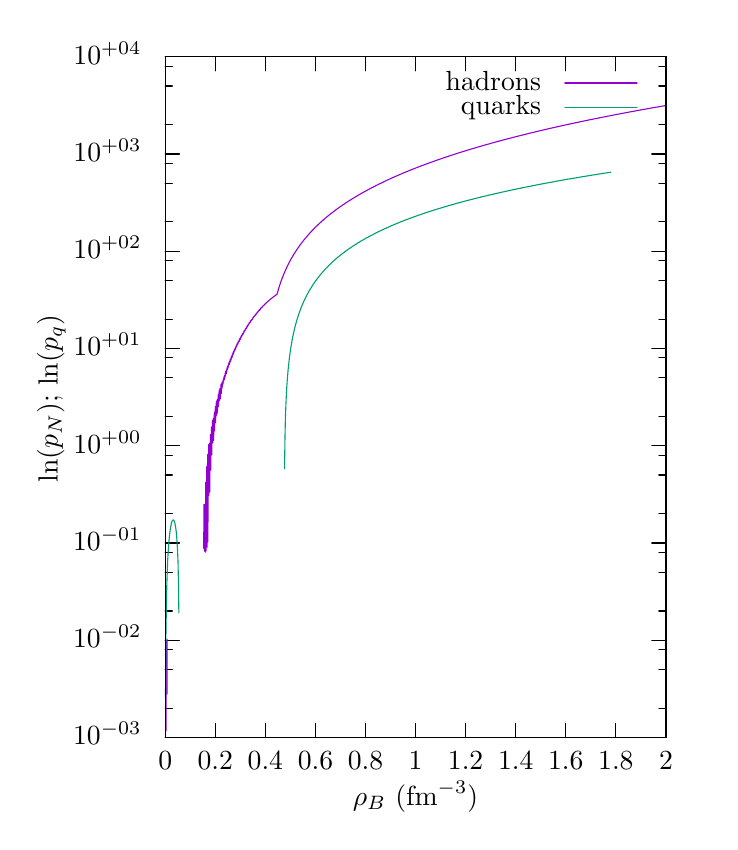
\begin{tikzpicture}[gnuplot]
%% generated with GNUPLOT 5.0p4 (Lua 5.2; terminal rev. 99, script rev. 100)
%% Thu Sep 29 16:33:18 2016
\path (0.000,0.000) rectangle (8.600,10.000);
\gpcolor{color=gp lt color border}
\gpsetlinetype{gp lt border}
\gpsetdashtype{gp dt solid}
\gpsetlinewidth{1.00}
\draw[gp path] (1.688,0.985)--(1.868,0.985);
\draw[gp path] (8.047,0.985)--(7.867,0.985);
\node[gp node right] at (1.504,0.985) {$10^{-03}$};
\draw[gp path] (1.688,1.357)--(1.778,1.357);
\draw[gp path] (8.047,1.357)--(7.957,1.357);
\draw[gp path] (1.688,1.848)--(1.778,1.848);
\draw[gp path] (8.047,1.848)--(7.957,1.848);
\draw[gp path] (1.688,2.100)--(1.778,2.100);
\draw[gp path] (8.047,2.100)--(7.957,2.100);
\draw[gp path] (1.688,2.220)--(1.868,2.220);
\draw[gp path] (8.047,2.220)--(7.867,2.220);
\node[gp node right] at (1.504,2.220) {$10^{-02}$};
\draw[gp path] (1.688,2.592)--(1.778,2.592);
\draw[gp path] (8.047,2.592)--(7.957,2.592);
\draw[gp path] (1.688,3.083)--(1.778,3.083);
\draw[gp path] (8.047,3.083)--(7.957,3.083);
\draw[gp path] (1.688,3.336)--(1.778,3.336);
\draw[gp path] (8.047,3.336)--(7.957,3.336);
\draw[gp path] (1.688,3.455)--(1.868,3.455);
\draw[gp path] (8.047,3.455)--(7.867,3.455);
\node[gp node right] at (1.504,3.455) {$10^{-01}$};
\draw[gp path] (1.688,3.827)--(1.778,3.827);
\draw[gp path] (8.047,3.827)--(7.957,3.827);
\draw[gp path] (1.688,4.319)--(1.778,4.319);
\draw[gp path] (8.047,4.319)--(7.957,4.319);
\draw[gp path] (1.688,4.571)--(1.778,4.571);
\draw[gp path] (8.047,4.571)--(7.957,4.571);
\draw[gp path] (1.688,4.690)--(1.868,4.690);
\draw[gp path] (8.047,4.690)--(7.867,4.690);
\node[gp node right] at (1.504,4.690) {$10^{+00}$};
\draw[gp path] (1.688,5.062)--(1.778,5.062);
\draw[gp path] (8.047,5.062)--(7.957,5.062);
\draw[gp path] (1.688,5.554)--(1.778,5.554);
\draw[gp path] (8.047,5.554)--(7.957,5.554);
\draw[gp path] (1.688,5.806)--(1.778,5.806);
\draw[gp path] (8.047,5.806)--(7.957,5.806);
\draw[gp path] (1.688,5.926)--(1.868,5.926);
\draw[gp path] (8.047,5.926)--(7.867,5.926);
\node[gp node right] at (1.504,5.926) {$10^{+01}$};
\draw[gp path] (1.688,6.297)--(1.778,6.297);
\draw[gp path] (8.047,6.297)--(7.957,6.297);
\draw[gp path] (1.688,6.789)--(1.778,6.789);
\draw[gp path] (8.047,6.789)--(7.957,6.789);
\draw[gp path] (1.688,7.041)--(1.778,7.041);
\draw[gp path] (8.047,7.041)--(7.957,7.041);
\draw[gp path] (1.688,7.161)--(1.868,7.161);
\draw[gp path] (8.047,7.161)--(7.867,7.161);
\node[gp node right] at (1.504,7.161) {$10^{+02}$};
\draw[gp path] (1.688,7.533)--(1.778,7.533);
\draw[gp path] (8.047,7.533)--(7.957,7.533);
\draw[gp path] (1.688,8.024)--(1.778,8.024);
\draw[gp path] (8.047,8.024)--(7.957,8.024);
\draw[gp path] (1.688,8.276)--(1.778,8.276);
\draw[gp path] (8.047,8.276)--(7.957,8.276);
\draw[gp path] (1.688,8.396)--(1.868,8.396);
\draw[gp path] (8.047,8.396)--(7.867,8.396);
\node[gp node right] at (1.504,8.396) {$10^{+03}$};
\draw[gp path] (1.688,8.768)--(1.778,8.768);
\draw[gp path] (8.047,8.768)--(7.957,8.768);
\draw[gp path] (1.688,9.259)--(1.778,9.259);
\draw[gp path] (8.047,9.259)--(7.957,9.259);
\draw[gp path] (1.688,9.511)--(1.778,9.511);
\draw[gp path] (8.047,9.511)--(7.957,9.511);
\draw[gp path] (1.688,9.631)--(1.868,9.631);
\draw[gp path] (8.047,9.631)--(7.867,9.631);
\node[gp node right] at (1.504,9.631) {$10^{+04}$};
\draw[gp path] (1.688,0.985)--(1.688,1.165);
\draw[gp path] (1.688,9.631)--(1.688,9.451);
\node[gp node center] at (1.688,0.677) {$0$};
\draw[gp path] (2.324,0.985)--(2.324,1.165);
\draw[gp path] (2.324,9.631)--(2.324,9.451);
\node[gp node center] at (2.324,0.677) {$0.2$};
\draw[gp path] (2.960,0.985)--(2.960,1.165);
\draw[gp path] (2.960,9.631)--(2.960,9.451);
\node[gp node center] at (2.960,0.677) {$0.4$};
\draw[gp path] (3.596,0.985)--(3.596,1.165);
\draw[gp path] (3.596,9.631)--(3.596,9.451);
\node[gp node center] at (3.596,0.677) {$0.6$};
\draw[gp path] (4.232,0.985)--(4.232,1.165);
\draw[gp path] (4.232,9.631)--(4.232,9.451);
\node[gp node center] at (4.232,0.677) {$0.8$};
\draw[gp path] (4.868,0.985)--(4.868,1.165);
\draw[gp path] (4.868,9.631)--(4.868,9.451);
\node[gp node center] at (4.868,0.677) {$1$};
\draw[gp path] (5.503,0.985)--(5.503,1.165);
\draw[gp path] (5.503,9.631)--(5.503,9.451);
\node[gp node center] at (5.503,0.677) {$1.2$};
\draw[gp path] (6.139,0.985)--(6.139,1.165);
\draw[gp path] (6.139,9.631)--(6.139,9.451);
\node[gp node center] at (6.139,0.677) {$1.4$};
\draw[gp path] (6.775,0.985)--(6.775,1.165);
\draw[gp path] (6.775,9.631)--(6.775,9.451);
\node[gp node center] at (6.775,0.677) {$1.6$};
\draw[gp path] (7.411,0.985)--(7.411,1.165);
\draw[gp path] (7.411,9.631)--(7.411,9.451);
\node[gp node center] at (7.411,0.677) {$1.8$};
\draw[gp path] (8.047,0.985)--(8.047,1.165);
\draw[gp path] (8.047,9.631)--(8.047,9.451);
\node[gp node center] at (8.047,0.677) {$2$};
\draw[gp path] (1.688,9.631)--(1.688,0.985)--(8.047,0.985)--(8.047,9.631)--cycle;
\node[gp node center,rotate=-270] at (0.246,5.308) {$\ln(p_N)$; $\ln(p_q)$};
\node[gp node center] at (4.867,0.215) {$\rho_B$ ($\rm{fm}^{-3}$)};
\node[gp node right] at (6.579,9.297) {hadrons};
\gpcolor{rgb color={0.580,0.000,0.827}}
\draw[gp path] (6.763,9.297)--(7.679,9.297);
\draw[gp path] (1.698,1.070)--(1.700,1.846)--(1.702,2.220);
\draw[gp path] (1.710,1.535)--(1.712,2.235);
\draw[gp path] (2.177,3.388)--(2.179,3.947);
\draw[gp path] (2.187,3.351)--(2.189,3.943);
\draw[gp path] (2.198,3.339)--(2.200,3.948)--(2.202,4.228);
\draw[gp path] (2.208,3.356)--(2.210,3.962)--(2.213,4.241)--(2.215,4.425);
\draw[gp path] (2.219,3.402)--(2.221,3.985)--(2.223,4.260)--(2.225,4.442)--(2.227,4.578)%
  --(2.229,3.471)--(2.232,4.017)--(2.234,4.284)--(2.236,4.462)--(2.238,4.597)--(2.240,4.705)%
  --(2.242,4.057)--(2.244,4.313)--(2.246,4.486)--(2.249,4.618)--(2.251,4.724)--(2.253,4.103)%
  --(2.255,4.346)--(2.257,4.513)--(2.259,4.642)--(2.261,4.746)--(2.263,4.834)--(2.266,4.383)%
  --(2.268,4.544)--(2.270,4.668)--(2.272,4.770)--(2.274,4.855)--(2.276,4.930)--(2.278,4.576)%
  --(2.280,4.696)--(2.282,4.795)--(2.285,4.879)--(2.287,4.952)--(2.289,5.016)--(2.291,4.727)%
  --(2.293,4.822)--(2.295,4.903)--(2.297,4.975)--(2.299,5.038)--(2.302,4.758)--(2.304,4.850)%
  --(2.306,4.929)--(2.308,4.999)--(2.310,5.060)--(2.312,5.116)--(2.314,4.880)--(2.316,4.957)%
  --(2.318,5.024)--(2.321,5.084)--(2.323,5.138)--(2.325,5.188)--(2.327,4.985)--(2.329,5.050)%
  --(2.331,5.108)--(2.333,5.161)--(2.335,5.210)--(2.338,5.255)--(2.340,5.077)--(2.342,5.134)%
  --(2.344,5.185)--(2.346,5.233)--(2.348,5.276)--(2.350,5.105)--(2.352,5.160)--(2.355,5.210)%
  --(2.357,5.256)--(2.359,5.299)--(2.361,5.338)--(2.363,5.186)--(2.365,5.235)--(2.367,5.280)%
  --(2.369,5.321)--(2.371,5.360)--(2.374,5.397)--(2.376,5.261)--(2.378,5.304)--(2.380,5.345)%
  --(2.382,5.383)--(2.384,5.418)--(2.386,5.287)--(2.388,5.329)--(2.391,5.368)--(2.393,5.405)%
  --(2.395,5.440)--(2.397,5.473)--(2.399,5.354)--(2.401,5.392)--(2.403,5.428)--(2.405,5.462)%
  --(2.408,5.494)--(2.410,5.420)--(2.412,5.454)--(2.414,5.487)--(2.416,5.449)--(2.418,5.482)%
  --(2.420,5.514)--(2.422,5.478)--(2.424,5.510)--(2.427,5.540)--(2.429,5.505)--(2.431,5.536)%
  --(2.433,5.565)--(2.435,5.532)--(2.437,5.562)--(2.439,5.529)--(2.441,5.559)--(2.444,5.587)%
  --(2.446,5.555)--(2.448,5.584)--(2.450,5.612)--(2.452,5.581)--(2.454,5.609)--(2.456,5.636)%
  --(2.458,5.607)--(2.460,5.633)--(2.463,5.604)--(2.465,5.631)--(2.467,5.657)--(2.469,5.629)%
  --(2.471,5.655)--(2.473,5.680)--(2.475,5.654)--(2.477,5.679)--(2.480,5.703)--(2.482,5.677)%
  --(2.484,5.702)--(2.486,5.676)--(2.488,5.701)--(2.490,5.724)--(2.492,5.700)--(2.494,5.723)%
  --(2.497,5.746)--(2.499,5.722)--(2.501,5.745)--(2.503,5.722)--(2.505,5.745)--(2.507,5.767)%
  --(2.509,5.744)--(2.511,5.767)--(2.513,5.788)--(2.516,5.767)--(2.518,5.788)--(2.520,5.766)%
  --(2.522,5.788)--(2.524,5.809)--(2.526,5.788)--(2.528,5.810)--(2.530,5.830)--(2.533,5.810)%
  --(2.535,5.830)--(2.537,5.810)--(2.539,5.831)--(2.541,5.851)--(2.543,5.831)--(2.545,5.851)%
  --(2.547,5.871)--(2.550,5.852)--(2.552,5.872)--(2.554,5.853)--(2.556,5.872)--(2.558,5.891)%
  --(2.560,5.873)--(2.562,5.892)--(2.564,5.911)--(2.566,5.894)--(2.569,5.912)--(2.571,5.895)%
  --(2.573,5.913)--(2.575,5.931)--(2.577,5.915)--(2.579,5.933)--(2.581,5.916)--(2.583,5.934)%
  --(2.586,5.952)--(2.588,5.936)--(2.590,5.953)--(2.592,5.970)--(2.594,5.955)--(2.596,5.972)%
  --(2.598,5.957)--(2.600,5.974)--(2.602,5.991)--(2.605,5.976)--(2.607,5.992)--(2.609,5.978)%
  --(2.611,5.995)--(2.613,6.011)--(2.615,5.997)--(2.617,6.013)--(2.619,5.999)--(2.622,6.015)%
  --(2.624,6.031)--(2.626,6.017)--(2.628,6.033)--(2.630,6.020)--(2.632,6.036)--(2.634,6.051)%
  --(2.636,6.038)--(2.639,6.053)--(2.641,6.041)--(2.643,6.056)--(2.645,6.071)--(2.647,6.059)%
  --(2.649,6.074)--(2.651,6.061)--(2.653,6.076)--(2.655,6.091)--(2.658,6.079)--(2.660,6.094)%
  --(2.662,6.082)--(2.664,6.097)--(2.666,6.111)--(2.668,6.100)--(2.670,6.114)--(2.672,6.103)%
  --(2.675,6.117)--(2.677,6.106)--(2.679,6.120)--(2.681,6.134)--(2.683,6.123)--(2.685,6.137)%
  --(2.687,6.127)--(2.689,6.141)--(2.691,6.154)--(2.694,6.144)--(2.696,6.157)--(2.698,6.147)%
  --(2.700,6.161)--(2.702,6.151)--(2.704,6.164)--(2.706,6.177)--(2.708,6.168)--(2.711,6.181)%
  --(2.713,6.171)--(2.715,6.185)--(2.717,6.175)--(2.719,6.188)--(2.721,6.201)--(2.723,6.192)%
  --(2.725,6.205)--(2.728,6.196)--(2.730,6.208)--(2.732,6.200)--(2.734,6.212)--(2.736,6.225)%
  --(2.738,6.216)--(2.740,6.229)--(2.742,6.220)--(2.744,6.233)--(2.747,6.224)--(2.749,6.237)%
  --(2.751,6.249)--(2.753,6.241)--(2.755,6.253)--(2.757,6.245)--(2.759,6.257)--(2.761,6.249)%
  --(2.764,6.261)--(2.766,6.253)--(2.768,6.265)--(2.770,6.258)--(2.772,6.270)--(2.774,6.281)%
  --(2.776,6.274)--(2.778,6.286)--(2.781,6.278)--(2.783,6.290)--(2.785,6.283)--(2.787,6.294)%
  --(2.789,6.288)--(2.791,6.299)--(2.793,6.292)--(2.795,6.304)--(2.797,6.297)--(2.800,6.308)%
  --(2.802,6.319)--(2.804,6.313)--(2.806,6.324)--(2.808,6.318)--(2.810,6.329)--(2.812,6.323)%
  --(2.814,6.334)--(2.817,6.328)--(2.819,6.338)--(2.821,6.333)--(2.823,6.343)--(2.825,6.338)%
  --(2.827,6.348)--(2.829,6.343)--(2.831,6.353)--(2.833,6.348)--(2.836,6.359)--(2.838,6.353)%
  --(2.840,6.364)--(2.842,6.358)--(2.844,6.369)--(2.846,6.364)--(2.848,6.374)--(2.850,6.369)%
  --(2.853,6.379)--(2.855,6.375)--(2.857,6.385)--(2.859,6.380)--(2.861,6.390)--(2.863,6.386)%
  --(2.865,6.396)--(2.867,6.391)--(2.870,6.401)--(2.872,6.397)--(2.874,6.407)--(2.876,6.403)%
  --(2.878,6.413)--(2.880,6.408)--(2.882,6.418)--(2.884,6.414)--(2.886,6.410)--(2.889,6.420)%
  --(2.891,6.416)--(2.893,6.426)--(2.895,6.422)--(2.897,6.432)--(2.899,6.428)--(2.901,6.438)%
  --(2.903,6.435)--(2.906,6.444)--(2.908,6.441)--(2.910,6.441)--(2.912,6.444)--(2.914,6.447)%
  --(2.916,6.450)--(2.918,6.453)--(2.920,6.456)--(2.923,6.453)--(2.925,6.457)--(2.927,6.460)%
  --(2.929,6.463)--(2.931,6.467)--(2.933,6.470)--(2.935,6.467)--(2.937,6.471)--(2.939,6.474)%
  --(2.942,6.477)--(2.944,6.475)--(2.946,6.478)--(2.948,6.482)--(2.950,6.485)--(2.952,6.489)%
  --(2.954,6.487)--(2.956,6.490)--(2.959,6.494)--(2.961,6.492)--(2.963,6.496)--(2.965,6.499)%
  --(2.967,6.503)--(2.969,6.501)--(2.971,6.505)--(2.973,6.509)--(2.975,6.507)--(2.978,6.511)%
  --(2.980,6.515)--(2.982,6.514)--(2.984,6.518)--(2.986,6.517)--(2.988,6.520)--(2.990,6.524)%
  --(2.992,6.524)--(2.995,6.528)--(2.997,6.527)--(2.999,6.531)--(3.001,6.530)--(3.003,6.534)%
  --(3.005,6.534)--(3.007,6.538)--(3.009,6.538)--(3.012,6.542)--(3.014,6.542)--(3.016,6.542)%
  --(3.018,6.547)--(3.020,6.547)--(3.022,6.551)--(3.024,6.551)--(3.026,6.552)--(3.028,6.556)%
  --(3.031,6.557)--(3.033,6.558)--(3.035,6.559)--(3.037,6.563)--(3.039,6.564)--(3.041,6.565)%
  --(3.043,6.567)--(3.045,6.568)--(3.048,6.569)--(3.050,6.571)--(3.052,6.572)--(3.054,6.574)%
  --(3.056,6.577)--(3.058,6.579)--(3.060,6.579)--(3.062,6.582)--(3.064,6.582)--(3.067,6.585)%
  --(3.069,6.586)--(3.071,6.587)--(3.073,6.589)--(3.075,6.591)--(3.077,6.593)--(3.079,6.594)%
  --(3.081,6.596)--(3.084,6.597)--(3.086,6.598)--(3.088,6.600)--(3.090,6.601)--(3.092,6.603)%
  --(3.094,6.604)--(3.096,6.606)--(3.098,6.607)--(3.101,6.609)--(3.103,6.610)--(3.105,6.611)%
  --(3.107,6.613)--(3.109,6.619)--(3.111,6.627)--(3.113,6.634)--(3.115,6.642)--(3.117,6.649)%
  --(3.120,6.657)--(3.122,6.664)--(3.124,6.671)--(3.126,6.678)--(3.128,6.685)--(3.130,6.692)%
  --(3.132,6.699)--(3.134,6.706)--(3.137,6.713)--(3.139,6.719)--(3.141,6.726)--(3.143,6.732)%
  --(3.145,6.739)--(3.147,6.745)--(3.149,6.751)--(3.151,6.757)--(3.154,6.764)--(3.156,6.770)%
  --(3.158,6.776)--(3.160,6.782)--(3.162,6.788)--(3.164,6.793)--(3.166,6.799)--(3.168,6.805)%
  --(3.170,6.811)--(3.173,6.816)--(3.175,6.822)--(3.177,6.827)--(3.179,6.833)--(3.181,6.838)%
  --(3.183,6.844)--(3.185,6.849)--(3.187,6.854)--(3.190,6.860)--(3.192,6.865)--(3.194,6.870)%
  --(3.196,6.875)--(3.198,6.880)--(3.200,6.885)--(3.202,6.890)--(3.204,6.895)--(3.206,6.900)%
  --(3.209,6.905)--(3.211,6.910)--(3.213,6.915)--(3.215,6.919)--(3.217,6.924)--(3.219,6.929)%
  --(3.221,6.933)--(3.223,6.938)--(3.226,6.943)--(3.228,6.947)--(3.230,6.952)--(3.232,6.956)%
  --(3.234,6.961)--(3.236,6.965)--(3.238,6.970)--(3.240,6.974)--(3.243,6.978)--(3.245,6.983)%
  --(3.247,6.987)--(3.249,6.991)--(3.251,6.995)--(3.253,7.000)--(3.255,7.004)--(3.257,7.008)%
  --(3.259,7.012)--(3.262,7.016)--(3.264,7.020)--(3.266,7.024)--(3.268,7.028)--(3.270,7.032)%
  --(3.272,7.036)--(3.274,7.040)--(3.276,7.044)--(3.279,7.048)--(3.281,7.052)--(3.283,7.056)%
  --(3.285,7.059)--(3.287,7.063)--(3.289,7.067)--(3.291,7.071)--(3.293,7.074)--(3.295,7.078)%
  --(3.298,7.082)--(3.300,7.085)--(3.302,7.089)--(3.304,7.093)--(3.306,7.096)--(3.308,7.100)%
  --(3.310,7.103)--(3.312,7.107)--(3.315,7.111)--(3.317,7.114)--(3.319,7.118)--(3.321,7.121)%
  --(3.323,7.124)--(3.325,7.128)--(3.327,7.131)--(3.329,7.135)--(3.332,7.138)--(3.334,7.141)%
  --(3.336,7.145)--(3.338,7.148)--(3.340,7.151)--(3.342,7.155)--(3.344,7.158)--(3.346,7.161)%
  --(3.348,7.165)--(3.351,7.168)--(3.353,7.171)--(3.355,7.174)--(3.357,7.177)--(3.359,7.181)%
  --(3.361,7.184)--(3.363,7.187)--(3.365,7.190)--(3.368,7.193)--(3.370,7.196)--(3.372,7.199)%
  --(3.374,7.202)--(3.376,7.205)--(3.378,7.208)--(3.380,7.212)--(3.382,7.215)--(3.385,7.218)%
  --(3.387,7.221)--(3.389,7.223)--(3.391,7.226)--(3.393,7.229)--(3.395,7.232)--(3.397,7.235)%
  --(3.399,7.238)--(3.401,7.241)--(3.404,7.244)--(3.406,7.247)--(3.408,7.250)--(3.410,7.253)%
  --(3.412,7.255)--(3.414,7.258)--(3.416,7.261)--(3.418,7.264)--(3.421,7.267)--(3.423,7.269)%
  --(3.425,7.272)--(3.427,7.275)--(3.429,7.278)--(3.431,7.280)--(3.433,7.283)--(3.435,7.286)%
  --(3.437,7.289)--(3.440,7.291)--(3.442,7.294)--(3.444,7.297)--(3.446,7.299)--(3.448,7.302)%
  --(3.450,7.305)--(3.452,7.307)--(3.454,7.310)--(3.457,7.312)--(3.459,7.315)--(3.461,7.318)%
  --(3.463,7.320)--(3.465,7.323)--(3.467,7.325)--(3.469,7.328)--(3.471,7.330)--(3.474,7.333)%
  --(3.476,7.335)--(3.478,7.338)--(3.480,7.340)--(3.482,7.343)--(3.484,7.345)--(3.486,7.348)%
  --(3.488,7.350)--(3.490,7.353)--(3.493,7.355)--(3.495,7.358)--(3.497,7.360)--(3.499,7.363)%
  --(3.501,7.365)--(3.503,7.367)--(3.505,7.370)--(3.507,7.372)--(3.510,7.375)--(3.512,7.377)%
  --(3.514,7.379)--(3.516,7.382)--(3.518,7.384)--(3.520,7.386)--(3.522,7.389)--(3.524,7.391)%
  --(3.527,7.393)--(3.529,7.396)--(3.531,7.398)--(3.533,7.400)--(3.535,7.403)--(3.537,7.405)%
  --(3.539,7.407)--(3.541,7.410)--(3.543,7.412)--(3.546,7.414)--(3.548,7.416)--(3.550,7.419)%
  --(3.552,7.421)--(3.554,7.423)--(3.556,7.425)--(3.558,7.427)--(3.560,7.430)--(3.563,7.432)%
  --(3.565,7.434)--(3.567,7.436)--(3.569,7.438)--(3.571,7.441)--(3.573,7.443)--(3.575,7.445)%
  --(3.577,7.447)--(3.579,7.449)--(3.582,7.451)--(3.584,7.454)--(3.586,7.456)--(3.588,7.458)%
  --(3.590,7.460)--(3.592,7.462)--(3.594,7.464)--(3.596,7.466)--(3.599,7.468)--(3.601,7.470)%
  --(3.603,7.473)--(3.605,7.475)--(3.607,7.477)--(3.609,7.479)--(3.611,7.481)--(3.613,7.483)%
  --(3.616,7.485)--(3.618,7.487)--(3.620,7.489)--(3.622,7.491)--(3.624,7.493)--(3.626,7.495)%
  --(3.628,7.497)--(3.630,7.499)--(3.632,7.501)--(3.635,7.503)--(3.637,7.505)--(3.639,7.507)%
  --(3.641,7.509)--(3.643,7.511)--(3.645,7.513)--(3.647,7.515)--(3.649,7.517)--(3.652,7.519)%
  --(3.654,7.521)--(3.656,7.523)--(3.658,7.525)--(3.660,7.527)--(3.662,7.528)--(3.664,7.530)%
  --(3.666,7.532)--(3.668,7.534)--(3.671,7.536)--(3.673,7.538)--(3.675,7.540)--(3.677,7.542)%
  --(3.679,7.544)--(3.681,7.546)--(3.683,7.548)--(3.685,7.549)--(3.688,7.551)--(3.690,7.553)%
  --(3.692,7.555)--(3.694,7.557)--(3.696,7.559)--(3.698,7.561)--(3.700,7.562)--(3.702,7.564)%
  --(3.705,7.566)--(3.707,7.568)--(3.709,7.570)--(3.711,7.572)--(3.713,7.573)--(3.715,7.575)%
  --(3.717,7.577)--(3.719,7.579)--(3.721,7.581)--(3.724,7.582)--(3.726,7.584)--(3.728,7.586)%
  --(3.730,7.588)--(3.732,7.589)--(3.734,7.591)--(3.736,7.593)--(3.738,7.595)--(3.741,7.597)%
  --(3.743,7.598)--(3.745,7.600)--(3.747,7.602)--(3.749,7.604)--(3.751,7.605)--(3.753,7.607)%
  --(3.755,7.609)--(3.758,7.610)--(3.760,7.612)--(3.762,7.614)--(3.764,7.616)--(3.766,7.617)%
  --(3.768,7.619)--(3.770,7.621)--(3.772,7.622)--(3.774,7.624)--(3.777,7.626)--(3.779,7.628)%
  --(3.781,7.629)--(3.783,7.631)--(3.785,7.633)--(3.787,7.634)--(3.789,7.636)--(3.791,7.638)%
  --(3.794,7.639)--(3.796,7.641)--(3.798,7.643)--(3.800,7.644)--(3.802,7.646)--(3.804,7.648)%
  --(3.806,7.649)--(3.808,7.651)--(3.810,7.652)--(3.813,7.654)--(3.815,7.656)--(3.817,7.657)%
  --(3.819,7.659)--(3.821,7.661)--(3.823,7.662)--(3.825,7.664)--(3.827,7.665)--(3.830,7.667)%
  --(3.832,7.669)--(3.834,7.670)--(3.836,7.672)--(3.838,7.673)--(3.840,7.675)--(3.842,7.677)%
  --(3.844,7.678)--(3.847,7.680)--(3.849,7.681)--(3.851,7.683)--(3.853,7.684)--(3.855,7.686)%
  --(3.857,7.688)--(3.859,7.689)--(3.861,7.691)--(3.863,7.692)--(3.866,7.694)--(3.868,7.695)%
  --(3.870,7.697)--(3.872,7.698)--(3.874,7.700)--(3.876,7.701)--(3.878,7.703)--(3.880,7.705)%
  --(3.883,7.706)--(3.885,7.708)--(3.887,7.709)--(3.889,7.711)--(3.891,7.712)--(3.893,7.714)%
  --(3.895,7.715)--(3.897,7.717)--(3.900,7.718)--(3.902,7.720)--(3.904,7.721)--(3.906,7.723)%
  --(3.908,7.724)--(3.910,7.726)--(3.912,7.727)--(3.914,7.729)--(3.916,7.730)--(3.919,7.732)%
  --(3.921,7.733)--(3.923,7.734)--(3.925,7.736)--(3.927,7.737)--(3.929,7.739)--(3.931,7.740)%
  --(3.933,7.742)--(3.936,7.743)--(3.938,7.745)--(3.940,7.746)--(3.942,7.748)--(3.944,7.749)%
  --(3.946,7.750)--(3.948,7.752)--(3.950,7.753)--(3.952,7.755)--(3.955,7.756)--(3.957,7.758)%
  --(3.959,7.759)--(3.961,7.760)--(3.963,7.762)--(3.965,7.763)--(3.967,7.765)--(3.969,7.766)%
  --(3.972,7.768)--(3.974,7.769)--(3.976,7.770)--(3.978,7.772)--(3.980,7.773)--(3.982,7.775)%
  --(3.984,7.776)--(3.986,7.777)--(3.989,7.779)--(3.991,7.780)--(3.993,7.782)--(3.995,7.783)%
  --(3.997,7.784)--(3.999,7.786)--(4.001,7.787)--(4.003,7.788)--(4.005,7.790)--(4.008,7.791)%
  --(4.010,7.793)--(4.012,7.794)--(4.014,7.795)--(4.016,7.797)--(4.018,7.798)--(4.020,7.799)%
  --(4.022,7.801)--(4.025,7.802)--(4.027,7.803)--(4.029,7.805)--(4.031,7.806)--(4.033,7.807)%
  --(4.035,7.809)--(4.037,7.810)--(4.039,7.811)--(4.041,7.813)--(4.044,7.814)--(4.046,7.815)%
  --(4.048,7.817)--(4.050,7.818)--(4.052,7.819)--(4.054,7.821)--(4.056,7.822)--(4.058,7.823)%
  --(4.061,7.825)--(4.063,7.826)--(4.065,7.827)--(4.067,7.829)--(4.069,7.830)--(4.071,7.831)%
  --(4.073,7.832)--(4.075,7.834)--(4.078,7.835)--(4.080,7.836)--(4.082,7.838)--(4.084,7.839)%
  --(4.086,7.840)--(4.088,7.842)--(4.090,7.843)--(4.092,7.844)--(4.094,7.845)--(4.097,7.847)%
  --(4.099,7.848)--(4.101,7.849)--(4.103,7.850)--(4.105,7.852)--(4.107,7.853)--(4.109,7.854)%
  --(4.111,7.856)--(4.114,7.857)--(4.116,7.858)--(4.118,7.859)--(4.120,7.861)--(4.122,7.862)%
  --(4.124,7.863)--(4.126,7.864)--(4.128,7.866)--(4.131,7.867)--(4.133,7.868)--(4.135,7.869)%
  --(4.137,7.871)--(4.139,7.872)--(4.141,7.873)--(4.143,7.874)--(4.145,7.876)--(4.147,7.877)%
  --(4.150,7.878)--(4.152,7.879)--(4.154,7.880)--(4.156,7.882)--(4.158,7.883)--(4.160,7.884)%
  --(4.162,7.885)--(4.164,7.887)--(4.167,7.888)--(4.169,7.889)--(4.171,7.890)--(4.173,7.891)%
  --(4.175,7.893)--(4.177,7.894)--(4.179,7.895)--(4.181,7.896)--(4.183,7.897)--(4.186,7.899)%
  --(4.188,7.900)--(4.190,7.901)--(4.192,7.902)--(4.194,7.903)--(4.196,7.905)--(4.198,7.906)%
  --(4.200,7.907)--(4.203,7.908)--(4.205,7.909)--(4.207,7.911)--(4.209,7.912)--(4.211,7.913)%
  --(4.213,7.914)--(4.215,7.915)--(4.217,7.916)--(4.220,7.918)--(4.222,7.919)--(4.224,7.920)%
  --(4.226,7.921)--(4.228,7.922)--(4.230,7.923)--(4.232,7.925)--(4.234,7.926)--(4.236,7.927)%
  --(4.239,7.928)--(4.241,7.929)--(4.243,7.930)--(4.245,7.932)--(4.247,7.933)--(4.249,7.934)%
  --(4.251,7.935)--(4.253,7.936)--(4.256,7.937)--(4.258,7.938)--(4.260,7.940)--(4.262,7.941)%
  --(4.264,7.942)--(4.266,7.943)--(4.268,7.944)--(4.270,7.945)--(4.273,7.946)--(4.275,7.948)%
  --(4.277,7.949)--(4.279,7.950)--(4.281,7.951)--(4.283,7.952)--(4.285,7.953)--(4.287,7.954)%
  --(4.289,7.955)--(4.292,7.957)--(4.294,7.958)--(4.296,7.959)--(4.298,7.960)--(4.300,7.961)%
  --(4.302,7.962)--(4.304,7.963)--(4.306,7.964)--(4.309,7.965)--(4.311,7.967)--(4.313,7.968)%
  --(4.315,7.969)--(4.317,7.970)--(4.319,7.971)--(4.321,7.972)--(4.323,7.973)--(4.325,7.974)%
  --(4.328,7.975)--(4.330,7.976)--(4.332,7.978)--(4.334,7.979)--(4.336,7.980)--(4.338,7.981)%
  --(4.340,7.982)--(4.342,7.983)--(4.345,7.984)--(4.347,7.985)--(4.349,7.986)--(4.351,7.987)%
  --(4.353,7.988)--(4.355,7.989)--(4.357,7.990)--(4.359,7.992)--(4.362,7.993)--(4.364,7.994)%
  --(4.366,7.995)--(4.368,7.996)--(4.370,7.997)--(4.372,7.998)--(4.374,7.999)--(4.376,8.000)%
  --(4.378,8.001)--(4.381,8.002)--(4.383,8.003)--(4.385,8.004)--(4.387,8.005)--(4.389,8.006)%
  --(4.391,8.008)--(4.393,8.009)--(4.395,8.010)--(4.398,8.011)--(4.400,8.012)--(4.402,8.013)%
  --(4.404,8.014)--(4.406,8.015)--(4.408,8.016)--(4.410,8.017)--(4.412,8.018)--(4.414,8.019)%
  --(4.417,8.020)--(4.419,8.021)--(4.421,8.022)--(4.423,8.023)--(4.425,8.024)--(4.427,8.025)%
  --(4.429,8.026)--(4.431,8.027)--(4.434,8.028)--(4.436,8.029)--(4.438,8.030)--(4.440,8.031)%
  --(4.442,8.032)--(4.444,8.033)--(4.446,8.034)--(4.448,8.035)--(4.451,8.037)--(4.453,8.038)%
  --(4.455,8.039)--(4.457,8.040)--(4.459,8.041)--(4.461,8.042)--(4.463,8.043)--(4.465,8.044)%
  --(4.467,8.045)--(4.470,8.046)--(4.472,8.047)--(4.474,8.048)--(4.476,8.049)--(4.478,8.050)%
  --(4.480,8.051)--(4.482,8.052)--(4.484,8.053)--(4.487,8.054)--(4.489,8.055)--(4.491,8.056)%
  --(4.493,8.057)--(4.495,8.058)--(4.497,8.059)--(4.499,8.060)--(4.501,8.061)--(4.504,8.062)%
  --(4.506,8.063)--(4.508,8.064)--(4.510,8.065)--(4.512,8.066)--(4.514,8.067)--(4.516,8.068)%
  --(4.518,8.068)--(4.520,8.069)--(4.523,8.070)--(4.525,8.071)--(4.527,8.072)--(4.529,8.073)%
  --(4.531,8.074)--(4.533,8.075)--(4.535,8.076)--(4.537,8.077)--(4.540,8.078)--(4.542,8.079)%
  --(4.544,8.080)--(4.546,8.081)--(4.548,8.082)--(4.550,8.083)--(4.552,8.084)--(4.554,8.085)%
  --(4.556,8.086)--(4.559,8.087)--(4.561,8.088)--(4.563,8.089)--(4.565,8.090)--(4.567,8.091)%
  --(4.569,8.092)--(4.571,8.093)--(4.573,8.094)--(4.576,8.095)--(4.578,8.096)--(4.580,8.096)%
  --(4.582,8.097)--(4.584,8.098)--(4.586,8.099)--(4.588,8.100)--(4.590,8.101)--(4.593,8.102)%
  --(4.595,8.103)--(4.597,8.104)--(4.599,8.105)--(4.601,8.106)--(4.603,8.107)--(4.605,8.108)%
  --(4.607,8.109)--(4.609,8.110)--(4.612,8.111)--(4.614,8.112)--(4.616,8.112)--(4.618,8.113)%
  --(4.620,8.114)--(4.622,8.115)--(4.624,8.116)--(4.626,8.117)--(4.629,8.118)--(4.631,8.119)%
  --(4.633,8.120)--(4.635,8.121)--(4.637,8.122)--(4.639,8.123)--(4.641,8.124)--(4.643,8.125)%
  --(4.646,8.125)--(4.648,8.126)--(4.650,8.127)--(4.652,8.128)--(4.654,8.129)--(4.656,8.130)%
  --(4.658,8.131)--(4.660,8.132)--(4.662,8.133)--(4.665,8.134)--(4.667,8.135)--(4.669,8.135)%
  --(4.671,8.136)--(4.673,8.137)--(4.675,8.138)--(4.677,8.139)--(4.679,8.140)--(4.682,8.141)%
  --(4.684,8.142)--(4.686,8.143)--(4.688,8.144)--(4.690,8.145)--(4.692,8.145)--(4.694,8.146)%
  --(4.696,8.147)--(4.698,8.148)--(4.701,8.149)--(4.703,8.150)--(4.705,8.151)--(4.707,8.152)%
  --(4.709,8.153)--(4.711,8.153)--(4.713,8.154)--(4.715,8.155)--(4.718,8.156)--(4.720,8.157)%
  --(4.722,8.158)--(4.724,8.159)--(4.726,8.160)--(4.728,8.161)--(4.730,8.161)--(4.732,8.162)%
  --(4.735,8.163)--(4.737,8.164)--(4.739,8.165)--(4.741,8.166)--(4.743,8.167)--(4.745,8.168)%
  --(4.747,8.168)--(4.749,8.169)--(4.751,8.170)--(4.754,8.171)--(4.756,8.172)--(4.758,8.173)%
  --(4.760,8.174)--(4.762,8.175)--(4.764,8.175)--(4.766,8.176)--(4.768,8.177)--(4.771,8.178)%
  --(4.773,8.179)--(4.775,8.180)--(4.777,8.181)--(4.779,8.182)--(4.781,8.182)--(4.783,8.183)%
  --(4.785,8.184)--(4.787,8.185)--(4.790,8.186)--(4.792,8.187)--(4.794,8.188)--(4.796,8.188)%
  --(4.798,8.189)--(4.800,8.190)--(4.802,8.191)--(4.804,8.192)--(4.807,8.193)--(4.809,8.194)%
  --(4.811,8.194)--(4.813,8.195)--(4.815,8.196)--(4.817,8.197)--(4.819,8.198)--(4.821,8.199)%
  --(4.824,8.199)--(4.826,8.200)--(4.828,8.201)--(4.830,8.202)--(4.832,8.203)--(4.834,8.204)%
  --(4.836,8.205)--(4.838,8.205)--(4.840,8.206)--(4.843,8.207)--(4.845,8.208)--(4.847,8.209)%
  --(4.849,8.210)--(4.851,8.210)--(4.853,8.211)--(4.855,8.212)--(4.857,8.213)--(4.860,8.214)%
  --(4.862,8.215)--(4.864,8.215)--(4.866,8.216)--(4.868,8.217)--(4.870,8.218)--(4.872,8.219)%
  --(4.874,8.220)--(4.877,8.220)--(4.879,8.221)--(4.881,8.222)--(4.883,8.223)--(4.885,8.224)%
  --(4.887,8.224)--(4.889,8.225)--(4.891,8.226)--(4.893,8.227)--(4.896,8.228)--(4.898,8.229)%
  --(4.900,8.229)--(4.902,8.230)--(4.904,8.231)--(4.906,8.232)--(4.908,8.233)--(4.910,8.233)%
  --(4.913,8.234)--(4.915,8.235)--(4.917,8.236)--(4.919,8.237)--(4.921,8.238)--(4.923,8.238)%
  --(4.925,8.239)--(4.927,8.240)--(4.929,8.241)--(4.932,8.242)--(4.934,8.242)--(4.936,8.243)%
  --(4.938,8.244)--(4.940,8.245)--(4.942,8.246)--(4.944,8.246)--(4.946,8.247)--(4.949,8.248)%
  --(4.951,8.249)--(4.953,8.250)--(4.955,8.250)--(4.957,8.251)--(4.959,8.252)--(4.961,8.253)%
  --(4.963,8.254)--(4.966,8.254)--(4.968,8.255)--(4.970,8.256)--(4.972,8.257)--(4.974,8.258)%
  --(4.976,8.258)--(4.978,8.259)--(4.980,8.260)--(4.982,8.261)--(4.985,8.262)--(4.987,8.262)%
  --(4.989,8.263)--(4.991,8.264)--(4.993,8.265)--(4.995,8.265)--(4.997,8.266)--(4.999,8.267)%
  --(5.002,8.268)--(5.004,8.269)--(5.006,8.269)--(5.008,8.270)--(5.010,8.271)--(5.012,8.272)%
  --(5.014,8.273)--(5.016,8.273)--(5.019,8.274)--(5.021,8.275)--(5.023,8.276)--(5.025,8.276)%
  --(5.027,8.277)--(5.029,8.278)--(5.031,8.279)--(5.033,8.279)--(5.035,8.280)--(5.038,8.281)%
  --(5.040,8.282)--(5.042,8.283)--(5.044,8.283)--(5.046,8.284)--(5.048,8.285)--(5.050,8.286)%
  --(5.052,8.286)--(5.055,8.287)--(5.057,8.288)--(5.059,8.289)--(5.061,8.290)--(5.063,8.290)%
  --(5.065,8.291)--(5.067,8.292)--(5.069,8.293)--(5.071,8.293)--(5.074,8.294)--(5.076,8.295)%
  --(5.078,8.296)--(5.080,8.296)--(5.082,8.297)--(5.084,8.298)--(5.086,8.299)--(5.088,8.299)%
  --(5.091,8.300)--(5.093,8.301)--(5.095,8.302)--(5.097,8.302)--(5.099,8.303)--(5.101,8.304)%
  --(5.103,8.305)--(5.105,8.305)--(5.108,8.306)--(5.110,8.307)--(5.112,8.308)--(5.114,8.308)%
  --(5.116,8.309)--(5.118,8.310)--(5.120,8.311)--(5.122,8.311)--(5.124,8.312)--(5.127,8.313)%
  --(5.129,8.314)--(5.131,8.314)--(5.133,8.315)--(5.135,8.316)--(5.137,8.317)--(5.139,8.317)%
  --(5.141,8.318)--(5.144,8.319)--(5.146,8.320)--(5.148,8.320)--(5.150,8.321)--(5.152,8.322)%
  --(5.154,8.323)--(5.156,8.323)--(5.158,8.324)--(5.160,8.325)--(5.163,8.326)--(5.165,8.326)%
  --(5.167,8.327)--(5.169,8.328)--(5.171,8.328)--(5.173,8.329)--(5.175,8.330)--(5.177,8.331)%
  --(5.180,8.331)--(5.182,8.332)--(5.184,8.333)--(5.186,8.334)--(5.188,8.334)--(5.190,8.335)%
  --(5.192,8.336)--(5.194,8.336)--(5.197,8.337)--(5.199,8.338)--(5.201,8.339)--(5.203,8.339)%
  --(5.205,8.340)--(5.207,8.341)--(5.209,8.342)--(5.211,8.342)--(5.213,8.343)--(5.216,8.344)%
  --(5.218,8.344)--(5.220,8.345)--(5.222,8.346)--(5.224,8.347)--(5.226,8.347)--(5.228,8.348)%
  --(5.230,8.349)--(5.233,8.349)--(5.235,8.350)--(5.237,8.351)--(5.239,8.352)--(5.241,8.352)%
  --(5.243,8.353)--(5.245,8.354)--(5.247,8.354)--(5.250,8.355)--(5.252,8.356)--(5.254,8.357)%
  --(5.256,8.357)--(5.258,8.358)--(5.260,8.359)--(5.262,8.359)--(5.264,8.360)--(5.266,8.361)%
  --(5.269,8.362)--(5.271,8.362)--(5.273,8.363)--(5.275,8.364)--(5.277,8.364)--(5.279,8.365)%
  --(5.281,8.366)--(5.283,8.367)--(5.286,8.367)--(5.288,8.368)--(5.290,8.369)--(5.292,8.369)%
  --(5.294,8.370)--(5.296,8.371)--(5.298,8.371)--(5.300,8.372)--(5.302,8.373)--(5.305,8.374)%
  --(5.307,8.374)--(5.309,8.375)--(5.311,8.376)--(5.313,8.376)--(5.315,8.377)--(5.317,8.378)%
  --(5.319,8.378)--(5.322,8.379)--(5.324,8.380)--(5.326,8.381)--(5.328,8.381)--(5.330,8.382)%
  --(5.332,8.383)--(5.334,8.383)--(5.336,8.384)--(5.339,8.385)--(5.341,8.385)--(5.343,8.386)%
  --(5.345,8.387)--(5.347,8.387)--(5.349,8.388)--(5.351,8.389)--(5.353,8.389)--(5.355,8.390)%
  --(5.358,8.391)--(5.360,8.392)--(5.362,8.392)--(5.364,8.393)--(5.366,8.394)--(5.368,8.394)%
  --(5.370,8.395)--(5.372,8.396)--(5.375,8.396)--(5.377,8.397)--(5.379,8.398)--(5.381,8.398)%
  --(5.383,8.399)--(5.385,8.400)--(5.387,8.400)--(5.389,8.401)--(5.392,8.402)--(5.394,8.402)%
  --(5.396,8.403)--(5.398,8.404)--(5.400,8.404)--(5.402,8.405)--(5.404,8.406)--(5.406,8.407)%
  --(5.408,8.407)--(5.411,8.408)--(5.413,8.409)--(5.415,8.409)--(5.417,8.410)--(5.419,8.411)%
  --(5.421,8.411)--(5.423,8.412)--(5.425,8.413)--(5.428,8.413)--(5.430,8.414)--(5.432,8.415)%
  --(5.434,8.415)--(5.436,8.416)--(5.438,8.417)--(5.440,8.417)--(5.442,8.418)--(5.444,8.419)%
  --(5.447,8.419)--(5.449,8.420)--(5.451,8.421)--(5.453,8.421)--(5.455,8.422)--(5.457,8.423)%
  --(5.459,8.423)--(5.461,8.424)--(5.464,8.425)--(5.466,8.425)--(5.468,8.426)--(5.470,8.427)%
  --(5.472,8.427)--(5.474,8.428)--(5.476,8.428)--(5.478,8.429)--(5.481,8.430)--(5.483,8.430)%
  --(5.485,8.431)--(5.487,8.432)--(5.489,8.432)--(5.491,8.433)--(5.493,8.434)--(5.495,8.434)%
  --(5.497,8.435)--(5.500,8.436)--(5.502,8.436)--(5.504,8.437)--(5.506,8.438)--(5.508,8.438)%
  --(5.510,8.439)--(5.512,8.440)--(5.514,8.440)--(5.517,8.441)--(5.519,8.442)--(5.521,8.442)%
  --(5.523,8.443)--(5.525,8.444)--(5.527,8.444)--(5.529,8.445)--(5.531,8.445)--(5.533,8.446)%
  --(5.536,8.447)--(5.538,8.447)--(5.540,8.448)--(5.542,8.449)--(5.544,8.449)--(5.546,8.450)%
  --(5.548,8.451)--(5.550,8.451)--(5.553,8.452)--(5.555,8.453)--(5.557,8.453)--(5.559,8.454)%
  --(5.561,8.454)--(5.563,8.455)--(5.565,8.456)--(5.567,8.456)--(5.570,8.457)--(5.572,8.458)%
  --(5.574,8.458)--(5.576,8.459)--(5.578,8.460)--(5.580,8.460)--(5.582,8.461)--(5.584,8.462)%
  --(5.586,8.462)--(5.589,8.463)--(5.591,8.463)--(5.593,8.464)--(5.595,8.465)--(5.597,8.465)%
  --(5.599,8.466)--(5.601,8.467)--(5.603,8.467)--(5.606,8.468)--(5.608,8.468)--(5.610,8.469)%
  --(5.612,8.470)--(5.614,8.470)--(5.616,8.471)--(5.618,8.472)--(5.620,8.472)--(5.623,8.473)%
  --(5.625,8.474)--(5.627,8.474)--(5.629,8.475)--(5.631,8.475)--(5.633,8.476)--(5.635,8.477)%
  --(5.637,8.477)--(5.639,8.478)--(5.642,8.479)--(5.644,8.479)--(5.646,8.480)--(5.648,8.480)%
  --(5.650,8.481)--(5.652,8.482)--(5.654,8.482)--(5.656,8.483)--(5.659,8.484)--(5.661,8.484)%
  --(5.663,8.485)--(5.665,8.485)--(5.667,8.486)--(5.669,8.487)--(5.671,8.487)--(5.673,8.488)%
  --(5.675,8.488)--(5.678,8.489)--(5.680,8.490)--(5.682,8.490)--(5.684,8.491)--(5.686,8.492)%
  --(5.688,8.492)--(5.690,8.493)--(5.692,8.493)--(5.695,8.494)--(5.697,8.495)--(5.699,8.495)%
  --(5.701,8.496)--(5.703,8.496)--(5.705,8.497)--(5.707,8.498)--(5.709,8.498)--(5.712,8.499)%
  --(5.714,8.500)--(5.716,8.500)--(5.718,8.501)--(5.720,8.501)--(5.722,8.502)--(5.724,8.503)%
  --(5.726,8.503)--(5.728,8.504)--(5.731,8.504)--(5.733,8.505)--(5.735,8.506)--(5.737,8.506)%
  --(5.739,8.507)--(5.741,8.507)--(5.743,8.508)--(5.745,8.509)--(5.748,8.509)--(5.750,8.510)%
  --(5.752,8.510)--(5.754,8.511)--(5.756,8.512)--(5.758,8.512)--(5.760,8.513)--(5.762,8.513)%
  --(5.764,8.514)--(5.767,8.515)--(5.769,8.515)--(5.771,8.516)--(5.773,8.516)--(5.775,8.517)%
  --(5.777,8.518)--(5.779,8.518)--(5.781,8.519)--(5.784,8.519)--(5.786,8.520)--(5.788,8.521)%
  --(5.790,8.521)--(5.792,8.522)--(5.794,8.522)--(5.796,8.523)--(5.798,8.524)--(5.801,8.524)%
  --(5.803,8.525)--(5.805,8.525)--(5.807,8.526)--(5.809,8.527)--(5.811,8.527)--(5.813,8.528)%
  --(5.815,8.528)--(5.817,8.529)--(5.820,8.530)--(5.822,8.530)--(5.824,8.531)--(5.826,8.531)%
  --(5.828,8.532)--(5.830,8.533)--(5.832,8.533)--(5.834,8.534)--(5.837,8.534)--(5.839,8.535)%
  --(5.841,8.536)--(5.843,8.536)--(5.845,8.537)--(5.847,8.537)--(5.849,8.538)--(5.851,8.538)%
  --(5.854,8.539)--(5.856,8.540)--(5.858,8.540)--(5.860,8.541)--(5.862,8.541)--(5.864,8.542)%
  --(5.866,8.543)--(5.868,8.543)--(5.870,8.544)--(5.873,8.544)--(5.875,8.545)--(5.877,8.545)%
  --(5.879,8.546)--(5.881,8.547)--(5.883,8.547)--(5.885,8.548)--(5.887,8.548)--(5.890,8.549)%
  --(5.892,8.550)--(5.894,8.550)--(5.896,8.551)--(5.898,8.551)--(5.900,8.552)--(5.902,8.552)%
  --(5.904,8.553)--(5.906,8.554)--(5.909,8.554)--(5.911,8.555)--(5.913,8.555)--(5.915,8.556)%
  --(5.917,8.556)--(5.919,8.557)--(5.921,8.558)--(5.923,8.558)--(5.926,8.559)--(5.928,8.559)%
  --(5.930,8.560)--(5.932,8.560)--(5.934,8.561)--(5.936,8.562)--(5.938,8.562)--(5.940,8.563)%
  --(5.943,8.563)--(5.945,8.564)--(5.947,8.564)--(5.949,8.565)--(5.951,8.566)--(5.953,8.566)%
  --(5.955,8.567)--(5.957,8.567)--(5.959,8.568)--(5.962,8.568)--(5.964,8.569)--(5.966,8.570)%
  --(5.968,8.570)--(5.970,8.571)--(5.972,8.571)--(5.974,8.572)--(5.976,8.572)--(5.979,8.573)%
  --(5.981,8.574)--(5.983,8.574)--(5.985,8.575)--(5.987,8.575)--(5.989,8.576)--(5.991,8.576)%
  --(5.993,8.577)--(5.996,8.578)--(5.998,8.578)--(6.000,8.579)--(6.002,8.579)--(6.004,8.580)%
  --(6.006,8.580)--(6.008,8.581)--(6.010,8.581)--(6.012,8.582)--(6.015,8.583)--(6.017,8.583)%
  --(6.019,8.584)--(6.021,8.584)--(6.023,8.585)--(6.025,8.585)--(6.027,8.586)--(6.029,8.587)%
  --(6.032,8.587)--(6.034,8.588)--(6.036,8.588)--(6.038,8.589)--(6.040,8.589)--(6.042,8.590)%
  --(6.044,8.590)--(6.046,8.591)--(6.048,8.592)--(6.051,8.592)--(6.053,8.593)--(6.055,8.593)%
  --(6.057,8.594)--(6.059,8.594)--(6.061,8.595)--(6.063,8.595)--(6.065,8.596)--(6.068,8.597)%
  --(6.070,8.597)--(6.072,8.598)--(6.074,8.598)--(6.076,8.599)--(6.078,8.599)--(6.080,8.600)%
  --(6.082,8.600)--(6.085,8.601)--(6.087,8.601)--(6.089,8.602)--(6.091,8.603)--(6.093,8.603)%
  --(6.095,8.604)--(6.097,8.604)--(6.099,8.605)--(6.101,8.605)--(6.104,8.606)--(6.106,8.606)%
  --(6.108,8.607)--(6.110,8.607)--(6.112,8.608)--(6.114,8.609)--(6.116,8.609)--(6.118,8.610)%
  --(6.121,8.610)--(6.123,8.611)--(6.125,8.611)--(6.127,8.612)--(6.129,8.612)--(6.131,8.613)%
  --(6.133,8.613)--(6.135,8.614)--(6.137,8.615)--(6.140,8.615)--(6.142,8.616)--(6.144,8.616)%
  --(6.146,8.617)--(6.148,8.617)--(6.150,8.618)--(6.152,8.618)--(6.154,8.619)--(6.157,8.619)%
  --(6.159,8.620)--(6.161,8.621)--(6.163,8.621)--(6.165,8.622)--(6.167,8.622)--(6.169,8.623)%
  --(6.171,8.623)--(6.174,8.624)--(6.176,8.624)--(6.178,8.625)--(6.180,8.625)--(6.182,8.626)%
  --(6.184,8.626)--(6.186,8.627)--(6.188,8.627)--(6.190,8.628)--(6.193,8.629)--(6.195,8.629)%
  --(6.197,8.630)--(6.199,8.630)--(6.201,8.631)--(6.203,8.631)--(6.205,8.632)--(6.207,8.632)%
  --(6.210,8.633)--(6.212,8.633)--(6.214,8.634)--(6.216,8.634)--(6.218,8.635)--(6.220,8.635)%
  --(6.222,8.636)--(6.224,8.637)--(6.227,8.637)--(6.229,8.638)--(6.231,8.638)--(6.233,8.639)%
  --(6.235,8.639)--(6.237,8.640)--(6.239,8.640)--(6.241,8.641)--(6.243,8.641)--(6.246,8.642)%
  --(6.248,8.642)--(6.250,8.643)--(6.252,8.643)--(6.254,8.644)--(6.256,8.644)--(6.258,8.645)%
  --(6.260,8.646)--(6.263,8.646)--(6.265,8.647)--(6.267,8.647)--(6.269,8.648)--(6.271,8.648)%
  --(6.273,8.649)--(6.275,8.649)--(6.277,8.650)--(6.279,8.650)--(6.282,8.651)--(6.284,8.651)%
  --(6.286,8.652)--(6.288,8.652)--(6.290,8.653)--(6.292,8.653)--(6.294,8.654)--(6.296,8.654)%
  --(6.299,8.655)--(6.301,8.655)--(6.303,8.656)--(6.305,8.656)--(6.307,8.657)--(6.309,8.658)%
  --(6.311,8.658)--(6.313,8.659)--(6.316,8.659)--(6.318,8.660)--(6.320,8.660)--(6.322,8.661)%
  --(6.324,8.661)--(6.326,8.662)--(6.328,8.662)--(6.330,8.663)--(6.332,8.663)--(6.335,8.664)%
  --(6.337,8.664)--(6.339,8.665)--(6.341,8.665)--(6.343,8.666)--(6.345,8.666)--(6.347,8.667)%
  --(6.349,8.667)--(6.352,8.668)--(6.354,8.668)--(6.356,8.669)--(6.358,8.669)--(6.360,8.670)%
  --(6.362,8.670)--(6.364,8.671)--(6.366,8.671)--(6.369,8.672)--(6.371,8.672)--(6.373,8.673)%
  --(6.375,8.673)--(6.377,8.674)--(6.379,8.674)--(6.381,8.675)--(6.383,8.675)--(6.385,8.676)%
  --(6.388,8.677)--(6.390,8.677)--(6.392,8.678)--(6.394,8.678)--(6.396,8.679)--(6.398,8.679)%
  --(6.400,8.680)--(6.402,8.680)--(6.405,8.681)--(6.407,8.681)--(6.409,8.682)--(6.411,8.682)%
  --(6.413,8.683)--(6.415,8.683)--(6.417,8.684)--(6.419,8.684)--(6.421,8.685)--(6.424,8.685)%
  --(6.426,8.686)--(6.428,8.686)--(6.430,8.687)--(6.432,8.687)--(6.434,8.688)--(6.436,8.688)%
  --(6.438,8.689)--(6.441,8.689)--(6.443,8.690)--(6.445,8.690)--(6.447,8.691)--(6.449,8.691)%
  --(6.451,8.692)--(6.453,8.692)--(6.455,8.693)--(6.458,8.693)--(6.460,8.694)--(6.462,8.694)%
  --(6.464,8.695)--(6.466,8.695)--(6.468,8.696)--(6.470,8.696)--(6.472,8.697)--(6.474,8.697)%
  --(6.477,8.698)--(6.479,8.698)--(6.481,8.699)--(6.483,8.699)--(6.485,8.700)--(6.487,8.700)%
  --(6.489,8.701)--(6.491,8.701)--(6.494,8.702)--(6.496,8.702)--(6.498,8.703)--(6.500,8.703)%
  --(6.502,8.704)--(6.504,8.704)--(6.506,8.705)--(6.508,8.705)--(6.510,8.706)--(6.513,8.706)%
  --(6.515,8.707)--(6.517,8.707)--(6.519,8.708)--(6.521,8.708)--(6.523,8.709)--(6.525,8.709)%
  --(6.527,8.710)--(6.530,8.710)--(6.532,8.711)--(6.534,8.711)--(6.536,8.711)--(6.538,8.712)%
  --(6.540,8.712)--(6.542,8.713)--(6.544,8.713)--(6.547,8.714)--(6.549,8.714)--(6.551,8.715)%
  --(6.553,8.715)--(6.555,8.716)--(6.557,8.716)--(6.559,8.717)--(6.561,8.717)--(6.563,8.718)%
  --(6.566,8.718)--(6.568,8.719)--(6.570,8.719)--(6.572,8.720)--(6.574,8.720)--(6.576,8.721)%
  --(6.578,8.721)--(6.580,8.722)--(6.583,8.722)--(6.585,8.723)--(6.587,8.723)--(6.589,8.724)%
  --(6.591,8.724)--(6.593,8.725)--(6.595,8.725)--(6.597,8.726)--(6.600,8.726)--(6.602,8.727)%
  --(6.604,8.727)--(6.606,8.728)--(6.608,8.728)--(6.610,8.729)--(6.612,8.729)--(6.614,8.729)%
  --(6.616,8.730)--(6.619,8.730)--(6.621,8.731)--(6.623,8.731)--(6.625,8.732)--(6.627,8.732)%
  --(6.629,8.733)--(6.631,8.733)--(6.633,8.734)--(6.636,8.734)--(6.638,8.735)--(6.640,8.735)%
  --(6.642,8.736)--(6.644,8.736)--(6.646,8.737)--(6.648,8.737)--(6.650,8.738)--(6.652,8.738)%
  --(6.655,8.739)--(6.657,8.739)--(6.659,8.740)--(6.661,8.740)--(6.663,8.741)--(6.665,8.741)%
  --(6.667,8.741)--(6.669,8.742)--(6.672,8.742)--(6.674,8.743)--(6.676,8.743)--(6.678,8.744)%
  --(6.680,8.744)--(6.682,8.745)--(6.684,8.745)--(6.686,8.746)--(6.689,8.746)--(6.691,8.747)%
  --(6.693,8.747)--(6.695,8.748)--(6.697,8.748)--(6.699,8.749)--(6.701,8.749)--(6.703,8.750)%
  --(6.705,8.750)--(6.708,8.750)--(6.710,8.751)--(6.712,8.751)--(6.714,8.752)--(6.716,8.752)%
  --(6.718,8.753)--(6.720,8.753)--(6.722,8.754)--(6.725,8.754)--(6.727,8.755)--(6.729,8.755)%
  --(6.731,8.756)--(6.733,8.756)--(6.735,8.757)--(6.737,8.757)--(6.739,8.758)--(6.742,8.758)%
  --(6.744,8.758)--(6.746,8.759)--(6.748,8.759)--(6.750,8.760)--(6.752,8.760)--(6.754,8.761)%
  --(6.756,8.761)--(6.758,8.762)--(6.761,8.762)--(6.763,8.763)--(6.765,8.763)--(6.767,8.764)%
  --(6.769,8.764)--(6.771,8.765)--(6.773,8.765)--(6.775,8.765)--(6.778,8.766)--(6.780,8.766)%
  --(6.782,8.767)--(6.784,8.767)--(6.786,8.768)--(6.788,8.768)--(6.790,8.769)--(6.792,8.769)%
  --(6.794,8.770)--(6.797,8.770)--(6.799,8.771)--(6.801,8.771)--(6.803,8.771)--(6.805,8.772)%
  --(6.807,8.772)--(6.809,8.773)--(6.811,8.773)--(6.814,8.774)--(6.816,8.774)--(6.818,8.775)%
  --(6.820,8.775)--(6.822,8.776)--(6.824,8.776)--(6.826,8.777)--(6.828,8.777)--(6.831,8.777)%
  --(6.833,8.778)--(6.835,8.778)--(6.837,8.779)--(6.839,8.779)--(6.841,8.780)--(6.843,8.780)%
  --(6.845,8.781)--(6.847,8.781)--(6.850,8.782)--(6.852,8.782)--(6.854,8.782)--(6.856,8.783)%
  --(6.858,8.783)--(6.860,8.784)--(6.862,8.784)--(6.864,8.785)--(6.867,8.785)--(6.869,8.786)%
  --(6.871,8.786)--(6.873,8.787)--(6.875,8.787)--(6.877,8.788)--(6.879,8.788)--(6.881,8.788)%
  --(6.883,8.789)--(6.886,8.789)--(6.888,8.790)--(6.890,8.790)--(6.892,8.791)--(6.894,8.791)%
  --(6.896,8.792)--(6.898,8.792)--(6.900,8.792)--(6.903,8.793)--(6.905,8.793)--(6.907,8.794)%
  --(6.909,8.794)--(6.911,8.795)--(6.913,8.795)--(6.915,8.796)--(6.917,8.796)--(6.920,8.797)%
  --(6.922,8.797)--(6.924,8.797)--(6.926,8.798)--(6.928,8.798)--(6.930,8.799)--(6.932,8.799)%
  --(6.934,8.800)--(6.936,8.800)--(6.939,8.801)--(6.941,8.801)--(6.943,8.801)--(6.945,8.802)%
  --(6.947,8.802)--(6.949,8.803)--(6.951,8.803)--(6.953,8.804)--(6.956,8.804)--(6.958,8.805)%
  --(6.960,8.805)--(6.962,8.806)--(6.964,8.806)--(6.966,8.806)--(6.968,8.807)--(6.970,8.807)%
  --(6.973,8.808)--(6.975,8.808)--(6.977,8.809)--(6.979,8.809)--(6.981,8.810)--(6.983,8.810)%
  --(6.985,8.810)--(6.987,8.811)--(6.989,8.811)--(6.992,8.812)--(6.994,8.812)--(6.996,8.813)%
  --(6.998,8.813)--(7.000,8.814)--(7.002,8.814)--(7.004,8.814)--(7.006,8.815)--(7.009,8.815)%
  --(7.011,8.816)--(7.013,8.816)--(7.015,8.817)--(7.017,8.817)--(7.019,8.817)--(7.021,8.818)%
  --(7.023,8.818)--(7.025,8.819)--(7.028,8.819)--(7.030,8.820)--(7.032,8.820)--(7.034,8.821)%
  --(7.036,8.821)--(7.038,8.821)--(7.040,8.822)--(7.042,8.822)--(7.045,8.823)--(7.047,8.823)%
  --(7.049,8.824)--(7.051,8.824)--(7.053,8.825)--(7.055,8.825)--(7.057,8.825)--(7.059,8.826)%
  --(7.062,8.826)--(7.064,8.827)--(7.066,8.827)--(7.068,8.828)--(7.070,8.828)--(7.072,8.828)%
  --(7.074,8.829)--(7.076,8.829)--(7.078,8.830)--(7.081,8.830)--(7.083,8.831)--(7.085,8.831)%
  --(7.087,8.832)--(7.089,8.832)--(7.091,8.832)--(7.093,8.833)--(7.095,8.833)--(7.098,8.834)%
  --(7.100,8.834)--(7.102,8.835)--(7.104,8.835)--(7.106,8.835)--(7.108,8.836)--(7.110,8.836)%
  --(7.112,8.837)--(7.115,8.837)--(7.117,8.838)--(7.119,8.838)--(7.121,8.838)--(7.123,8.839)%
  --(7.125,8.839)--(7.127,8.840)--(7.129,8.840)--(7.131,8.841)--(7.134,8.841)--(7.136,8.841)%
  --(7.138,8.842)--(7.140,8.842)--(7.142,8.843)--(7.144,8.843)--(7.146,8.844)--(7.148,8.844)%
  --(7.151,8.844)--(7.153,8.845)--(7.155,8.845)--(7.157,8.846)--(7.159,8.846)--(7.161,8.847)%
  --(7.163,8.847)--(7.165,8.847)--(7.167,8.848)--(7.170,8.848)--(7.172,8.849)--(7.174,8.849)%
  --(7.176,8.850)--(7.178,8.850)--(7.180,8.850)--(7.182,8.851)--(7.184,8.851)--(7.187,8.852)%
  --(7.189,8.852)--(7.191,8.853)--(7.193,8.853)--(7.195,8.853)--(7.197,8.854)--(7.199,8.854)%
  --(7.201,8.855)--(7.204,8.855)--(7.206,8.856)--(7.208,8.856)--(7.210,8.856)--(7.212,8.857)%
  --(7.214,8.857)--(7.216,8.858)--(7.218,8.858)--(7.220,8.859)--(7.223,8.859)--(7.225,8.859)%
  --(7.227,8.860)--(7.229,8.860)--(7.231,8.861)--(7.233,8.861)--(7.235,8.861)--(7.237,8.862)%
  --(7.240,8.862)--(7.242,8.863)--(7.244,8.863)--(7.246,8.864)--(7.248,8.864)--(7.250,8.864)%
  --(7.252,8.865)--(7.254,8.865)--(7.256,8.866)--(7.259,8.866)--(7.261,8.867)--(7.263,8.867)%
  --(7.265,8.867)--(7.267,8.868)--(7.269,8.868)--(7.271,8.869)--(7.273,8.869)--(7.276,8.869)%
  --(7.278,8.870)--(7.280,8.870)--(7.282,8.871)--(7.284,8.871)--(7.286,8.872)--(7.288,8.872)%
  --(7.290,8.872)--(7.293,8.873)--(7.295,8.873)--(7.297,8.874)--(7.299,8.874)--(7.301,8.874)%
  --(7.303,8.875)--(7.305,8.875)--(7.307,8.876)--(7.309,8.876)--(7.312,8.877)--(7.314,8.877)%
  --(7.316,8.877)--(7.318,8.878)--(7.320,8.878)--(7.322,8.879)--(7.324,8.879)--(7.326,8.879)%
  --(7.329,8.880)--(7.331,8.880)--(7.333,8.881)--(7.335,8.881)--(7.337,8.882)--(7.339,8.882)%
  --(7.341,8.882)--(7.343,8.883)--(7.346,8.883)--(7.348,8.884)--(7.350,8.884)--(7.352,8.884)%
  --(7.354,8.885)--(7.356,8.885)--(7.358,8.886)--(7.360,8.886)--(7.362,8.886)--(7.365,8.887)%
  --(7.367,8.887)--(7.369,8.888)--(7.371,8.888)--(7.373,8.889)--(7.375,8.889)--(7.377,8.889)%
  --(7.379,8.890)--(7.382,8.890)--(7.384,8.891)--(7.386,8.891)--(7.388,8.891)--(7.390,8.892)%
  --(7.392,8.892)--(7.394,8.893)--(7.396,8.893)--(7.398,8.893)--(7.401,8.894)--(7.403,8.894)%
  --(7.405,8.895)--(7.407,8.895)--(7.409,8.895)--(7.411,8.896)--(7.413,8.896)--(7.415,8.897)%
  --(7.418,8.897)--(7.420,8.898)--(7.422,8.898)--(7.424,8.898)--(7.426,8.899)--(7.428,8.899)%
  --(7.430,8.900)--(7.432,8.900)--(7.435,8.900)--(7.437,8.901)--(7.439,8.901)--(7.441,8.902)%
  --(7.443,8.902)--(7.445,8.902)--(7.447,8.903)--(7.449,8.903)--(7.451,8.904)--(7.454,8.904)%
  --(7.456,8.904)--(7.458,8.905)--(7.460,8.905)--(7.462,8.906)--(7.464,8.906)--(7.466,8.906)%
  --(7.468,8.907)--(7.471,8.907)--(7.473,8.908)--(7.475,8.908)--(7.477,8.908)--(7.479,8.909)%
  --(7.481,8.909)--(7.483,8.910)--(7.485,8.910)--(7.488,8.910)--(7.490,8.911)--(7.492,8.911)%
  --(7.494,8.912)--(7.496,8.912)--(7.498,8.912)--(7.500,8.913)--(7.502,8.913)--(7.504,8.914)%
  --(7.507,8.914)--(7.509,8.914)--(7.511,8.915)--(7.513,8.915)--(7.515,8.916)--(7.517,8.916)%
  --(7.519,8.916)--(7.521,8.917)--(7.524,8.917)--(7.526,8.918)--(7.528,8.918)--(7.530,8.918)%
  --(7.532,8.919)--(7.534,8.919)--(7.536,8.920)--(7.538,8.920)--(7.540,8.920)--(7.543,8.921)%
  --(7.545,8.921)--(7.547,8.922)--(7.549,8.922)--(7.551,8.922)--(7.553,8.923)--(7.555,8.923)%
  --(7.557,8.924)--(7.560,8.924)--(7.562,8.924)--(7.564,8.925)--(7.566,8.925)--(7.568,8.926)%
  --(7.570,8.926)--(7.572,8.926)--(7.574,8.927)--(7.577,8.927)--(7.579,8.928)--(7.581,8.928)%
  --(7.583,8.928)--(7.585,8.929)--(7.587,8.929)--(7.589,8.930)--(7.591,8.930)--(7.593,8.930)%
  --(7.596,8.931)--(7.598,8.931)--(7.600,8.932)--(7.602,8.932)--(7.604,8.932)--(7.606,8.933)%
  --(7.608,8.933)--(7.610,8.934)--(7.613,8.934)--(7.615,8.934)--(7.617,8.935)--(7.619,8.935)%
  --(7.621,8.935)--(7.623,8.936)--(7.625,8.936)--(7.627,8.937)--(7.629,8.937)--(7.632,8.937)%
  --(7.634,8.938)--(7.636,8.938)--(7.638,8.939)--(7.640,8.939)--(7.642,8.939)--(7.644,8.940)%
  --(7.646,8.940)--(7.649,8.941)--(7.651,8.941)--(7.653,8.941)--(7.655,8.942)--(7.657,8.942)%
  --(7.659,8.942)--(7.661,8.943)--(7.663,8.943)--(7.666,8.944)--(7.668,8.944)--(7.670,8.944)%
  --(7.672,8.945)--(7.674,8.945)--(7.676,8.946)--(7.678,8.946)--(7.680,8.946)--(7.682,8.947)%
  --(7.685,8.947)--(7.687,8.948)--(7.689,8.948)--(7.691,8.948)--(7.693,8.949)--(7.695,8.949)%
  --(7.697,8.949)--(7.699,8.950)--(7.702,8.950)--(7.704,8.951)--(7.706,8.951)--(7.708,8.951)%
  --(7.710,8.952)--(7.712,8.952)--(7.714,8.953)--(7.716,8.953)--(7.719,8.953)--(7.721,8.954)%
  --(7.723,8.954)--(7.725,8.954)--(7.727,8.955)--(7.729,8.955)--(7.731,8.956)--(7.733,8.956)%
  --(7.735,8.956)--(7.738,8.957)--(7.740,8.957)--(7.742,8.958)--(7.744,8.958)--(7.746,8.958)%
  --(7.748,8.959)--(7.750,8.959)--(7.752,8.959)--(7.755,8.960)--(7.757,8.960)--(7.759,8.961)%
  --(7.761,8.961)--(7.763,8.961)--(7.765,8.962)--(7.767,8.962)--(7.769,8.963)--(7.771,8.963)%
  --(7.774,8.963)--(7.776,8.964)--(7.778,8.964)--(7.780,8.964)--(7.782,8.965)--(7.784,8.965)%
  --(7.786,8.966)--(7.788,8.966)--(7.791,8.966)--(7.793,8.967)--(7.795,8.967)--(7.797,8.967)%
  --(7.799,8.968)--(7.801,8.968)--(7.803,8.969)--(7.805,8.969)--(7.808,8.969)--(7.810,8.970)%
  --(7.812,8.970)--(7.814,8.971)--(7.816,8.971)--(7.818,8.971)--(7.820,8.972)--(7.822,8.972)%
  --(7.824,8.972)--(7.827,8.973)--(7.829,8.973)--(7.831,8.974)--(7.833,8.974)--(7.835,8.974)%
  --(7.837,8.975)--(7.839,8.975)--(7.841,8.975)--(7.844,8.976)--(7.846,8.976)--(7.848,8.977)%
  --(7.850,8.977)--(7.852,8.977)--(7.854,8.978)--(7.856,8.978)--(7.858,8.978)--(7.861,8.979)%
  --(7.863,8.979)--(7.865,8.980)--(7.867,8.980)--(7.869,8.980)--(7.871,8.981)--(7.873,8.981)%
  --(7.875,8.981)--(7.877,8.982)--(7.880,8.982)--(7.882,8.983)--(7.884,8.983)--(7.886,8.983)%
  --(7.888,8.984)--(7.890,8.984)--(7.892,8.984)--(7.894,8.985)--(7.897,8.985)--(7.899,8.986)%
  --(7.901,8.986)--(7.903,8.986)--(7.905,8.987)--(7.907,8.987)--(7.909,8.987)--(7.911,8.988)%
  --(7.913,8.988)--(7.916,8.989)--(7.918,8.989)--(7.920,8.989)--(7.922,8.990)--(7.924,8.990)%
  --(7.926,8.990)--(7.928,8.991)--(7.930,8.991)--(7.933,8.991)--(7.935,8.992)--(7.937,8.992)%
  --(7.939,8.993)--(7.941,8.993)--(7.943,8.993)--(7.945,8.994)--(7.947,8.994)--(7.950,8.994)%
  --(7.952,8.995)--(7.954,8.995)--(7.956,8.996)--(7.958,8.996)--(7.960,8.996)--(7.962,8.997)%
  --(7.964,8.997)--(7.966,8.997)--(7.969,8.998)--(7.971,8.998)--(7.973,8.999)--(7.975,8.999)%
  --(7.977,8.999)--(7.979,9.000)--(7.981,9.000)--(7.983,9.000)--(7.986,9.001)--(7.988,9.001)%
  --(7.990,9.001)--(7.992,9.002)--(7.994,9.002)--(7.996,9.003)--(7.998,9.003)--(8.000,9.003)%
  --(8.002,9.004)--(8.005,9.004)--(8.007,9.004)--(8.009,9.005)--(8.011,9.005)--(8.013,9.005)%
  --(8.015,9.006)--(8.017,9.006)--(8.019,9.007)--(8.022,9.007)--(8.024,9.007)--(8.026,9.008)%
  --(8.028,9.008)--(8.030,9.008)--(8.032,9.009)--(8.034,9.009)--(8.036,9.009)--(8.039,9.010)%
  --(8.041,9.010)--(8.043,9.011)--(8.045,9.011)--(8.047,9.011);
\gpcolor{color=gp lt color border}
\node[gp node right] at (6.579,8.989) {quarks};
\gpcolor{rgb color={0.000,0.620,0.451}}
\draw[gp path] (6.763,8.989)--(7.679,8.989);
\draw[gp path] (1.691,1.486)--(1.697,2.308)--(1.703,2.685)--(1.708,2.928)--(1.714,3.099)%
  --(1.719,3.233)--(1.725,3.339)--(1.731,3.422)--(1.736,3.494)--(1.742,3.550)--(1.748,3.600)%
  --(1.753,3.639)--(1.759,3.671)--(1.765,3.700)--(1.770,3.720)--(1.776,3.734)--(1.782,3.743)%
  --(1.787,3.748)--(1.793,3.747)--(1.799,3.742)--(1.804,3.726)--(1.810,3.709)--(1.816,3.680)%
  --(1.821,3.650)--(1.827,3.603)--(1.833,3.543)--(1.838,3.467)--(1.844,3.366)--(1.850,3.227)%
  --(1.855,2.991)--(1.861,2.566);
\draw[gp path] (3.203,4.398)--(3.209,4.812)--(3.214,5.043)--(3.220,5.204)--(3.226,5.328)%
  --(3.231,5.429)--(3.237,5.513)--(3.243,5.587)--(3.248,5.651)--(3.254,5.709)--(3.260,5.761)%
  --(3.265,5.809)--(3.271,5.852)--(3.277,5.893)--(3.282,5.931)--(3.288,5.966)--(3.294,5.999)%
  --(3.299,6.030)--(3.305,6.060)--(3.311,6.088)--(3.316,6.115)--(3.322,6.140)--(3.327,6.164)%
  --(3.333,6.188)--(3.339,6.210)--(3.344,6.231)--(3.350,6.252)--(3.356,6.272)--(3.361,6.291)%
  --(3.367,6.310)--(3.373,6.328)--(3.378,6.345)--(3.384,6.362)--(3.390,6.378)--(3.395,6.394)%
  --(3.401,6.410)--(3.407,6.425)--(3.412,6.440)--(3.418,6.454)--(3.424,6.468)--(3.429,6.481)%
  --(3.435,6.495)--(3.441,6.508)--(3.446,6.520)--(3.452,6.533)--(3.458,6.545)--(3.463,6.557)%
  --(3.469,6.568)--(3.475,6.580)--(3.480,6.591)--(3.486,6.602)--(3.492,6.613)--(3.497,6.623)%
  --(3.503,6.634)--(3.509,6.644)--(3.514,6.654)--(3.520,6.664)--(3.526,6.673)--(3.531,6.683)%
  --(3.537,6.692)--(3.543,6.701)--(3.548,6.710)--(3.554,6.719)--(3.560,6.728)--(3.565,6.736)%
  --(3.571,6.745)--(3.577,6.753)--(3.582,6.762)--(3.588,6.770)--(3.594,6.778)--(3.599,6.786)%
  --(3.605,6.793)--(3.611,6.801)--(3.616,6.809)--(3.622,6.816)--(3.628,6.824)--(3.633,6.831)%
  --(3.639,6.838)--(3.645,6.845)--(3.650,6.852)--(3.656,6.859)--(3.662,6.866)--(3.667,6.873)%
  --(3.673,6.880)--(3.679,6.886)--(3.684,6.893)--(3.690,6.899)--(3.696,6.906)--(3.701,6.912)%
  --(3.707,6.919)--(3.713,6.925)--(3.718,6.931)--(3.724,6.937)--(3.729,6.943)--(3.735,6.949)%
  --(3.741,6.955)--(3.746,6.961)--(3.752,6.966)--(3.758,6.972)--(3.763,6.978)--(3.769,6.983)%
  --(3.775,6.989)--(3.780,6.995)--(3.786,7.000)--(3.792,7.005)--(3.797,7.011)--(3.803,7.016)%
  --(3.809,7.021)--(3.814,7.027)--(3.820,7.032)--(3.826,7.037)--(3.831,7.042)--(3.837,7.047)%
  --(3.843,7.052)--(3.848,7.057)--(3.854,7.062)--(3.860,7.067)--(3.865,7.072)--(3.871,7.076)%
  --(3.877,7.081)--(3.882,7.086)--(3.888,7.091)--(3.894,7.095)--(3.899,7.100)--(3.905,7.104)%
  --(3.911,7.109)--(3.916,7.113)--(3.922,7.118)--(3.928,7.122)--(3.933,7.127)--(3.939,7.131)%
  --(3.945,7.136)--(3.950,7.140)--(3.956,7.144)--(3.962,7.148)--(3.967,7.153)--(3.973,7.157)%
  --(3.979,7.161)--(3.984,7.165)--(3.990,7.169)--(3.996,7.173)--(4.001,7.177)--(4.007,7.181)%
  --(4.013,7.185)--(4.018,7.189)--(4.024,7.193)--(4.030,7.197)--(4.035,7.201)--(4.041,7.205)%
  --(4.047,7.209)--(4.052,7.213)--(4.058,7.216)--(4.064,7.220)--(4.069,7.224)--(4.075,7.228)%
  --(4.081,7.231)--(4.086,7.235)--(4.092,7.239)--(4.098,7.242)--(4.103,7.246)--(4.109,7.249)%
  --(4.115,7.253)--(4.120,7.257)--(4.126,7.260)--(4.131,7.264)--(4.137,7.267)--(4.143,7.271)%
  --(4.148,7.274)--(4.154,7.277)--(4.160,7.281)--(4.165,7.284)--(4.171,7.288)--(4.177,7.291)%
  --(4.182,7.294)--(4.188,7.298)--(4.194,7.301)--(4.199,7.304)--(4.205,7.308)--(4.211,7.311)%
  --(4.216,7.314)--(4.222,7.317)--(4.228,7.320)--(4.233,7.324)--(4.239,7.327)--(4.245,7.330)%
  --(4.250,7.333)--(4.256,7.336)--(4.262,7.339)--(4.267,7.342)--(4.273,7.345)--(4.279,7.348)%
  --(4.284,7.351)--(4.290,7.355)--(4.296,7.358)--(4.301,7.361)--(4.307,7.363)--(4.313,7.366)%
  --(4.318,7.369)--(4.324,7.372)--(4.330,7.375)--(4.335,7.378)--(4.341,7.381)--(4.347,7.384)%
  --(4.352,7.387)--(4.358,7.390)--(4.364,7.393)--(4.369,7.395)--(4.375,7.398)--(4.381,7.401)%
  --(4.386,7.404)--(4.392,7.407)--(4.398,7.409)--(4.403,7.412)--(4.409,7.415)--(4.415,7.418)%
  --(4.420,7.420)--(4.426,7.423)--(4.432,7.426)--(4.437,7.428)--(4.443,7.431)--(4.449,7.434)%
  --(4.454,7.436)--(4.460,7.439)--(4.466,7.442)--(4.471,7.444)--(4.477,7.447)--(4.483,7.449)%
  --(4.488,7.452)--(4.494,7.455)--(4.500,7.457)--(4.505,7.460)--(4.511,7.462)--(4.517,7.465)%
  --(4.522,7.467)--(4.528,7.470)--(4.533,7.472)--(4.539,7.475)--(4.545,7.477)--(4.550,7.480)%
  --(4.556,7.482)--(4.562,7.485)--(4.567,7.487)--(4.573,7.490)--(4.579,7.492)--(4.584,7.494)%
  --(4.590,7.497)--(4.596,7.499)--(4.601,7.502)--(4.607,7.504)--(4.613,7.506)--(4.618,7.509)%
  --(4.624,7.511)--(4.630,7.513)--(4.635,7.516)--(4.641,7.518)--(4.647,7.520)--(4.652,7.523)%
  --(4.658,7.525)--(4.664,7.527)--(4.669,7.529)--(4.675,7.532)--(4.681,7.534)--(4.686,7.536)%
  --(4.692,7.539)--(4.698,7.541)--(4.703,7.543)--(4.709,7.545)--(4.715,7.547)--(4.720,7.550)%
  --(4.726,7.552)--(4.732,7.554)--(4.737,7.556)--(4.743,7.558)--(4.749,7.561)--(4.754,7.563)%
  --(4.760,7.565)--(4.766,7.567)--(4.771,7.569)--(4.777,7.571)--(4.783,7.573)--(4.788,7.576)%
  --(4.794,7.578)--(4.800,7.580)--(4.805,7.582)--(4.811,7.584)--(4.817,7.586)--(4.822,7.588)%
  --(4.828,7.590)--(4.834,7.592)--(4.839,7.594)--(4.845,7.596)--(4.851,7.598)--(4.856,7.601)%
  --(4.862,7.603)--(4.868,7.605)--(4.873,7.607)--(4.879,7.609)--(4.885,7.611)--(4.890,7.613)%
  --(4.896,7.615)--(4.902,7.617)--(4.907,7.619)--(4.913,7.621)--(4.919,7.623)--(4.924,7.624)%
  --(4.930,7.626)--(4.936,7.628)--(4.941,7.630)--(4.947,7.632)--(4.952,7.634)--(4.958,7.636)%
  --(4.964,7.638)--(4.969,7.640)--(4.975,7.642)--(4.981,7.644)--(4.986,7.646)--(4.992,7.648)%
  --(4.998,7.649)--(5.003,7.651)--(5.009,7.653)--(5.015,7.655)--(5.020,7.657)--(5.026,7.659)%
  --(5.032,7.661)--(5.037,7.663)--(5.043,7.664)--(5.049,7.666)--(5.054,7.668)--(5.060,7.670)%
  --(5.066,7.672)--(5.071,7.674)--(5.077,7.675)--(5.083,7.677)--(5.088,7.679)--(5.094,7.681)%
  --(5.100,7.683)--(5.105,7.684)--(5.111,7.686)--(5.117,7.688)--(5.122,7.690)--(5.128,7.691)%
  --(5.134,7.693)--(5.139,7.695)--(5.145,7.697)--(5.151,7.698)--(5.156,7.700)--(5.162,7.702)%
  --(5.168,7.704)--(5.173,7.705)--(5.179,7.707)--(5.185,7.709)--(5.190,7.711)--(5.196,7.712)%
  --(5.202,7.714)--(5.207,7.716)--(5.213,7.717)--(5.219,7.719)--(5.224,7.721)--(5.230,7.722)%
  --(5.236,7.724)--(5.241,7.726)--(5.247,7.728)--(5.253,7.729)--(5.258,7.731)--(5.264,7.733)%
  --(5.270,7.734)--(5.275,7.736)--(5.281,7.737)--(5.287,7.739)--(5.292,7.741)--(5.298,7.742)%
  --(5.304,7.744)--(5.309,7.746)--(5.315,7.747)--(5.321,7.749)--(5.326,7.751)--(5.332,7.752)%
  --(5.338,7.754)--(5.343,7.755)--(5.349,7.757)--(5.354,7.759)--(5.360,7.760)--(5.366,7.762)%
  --(5.371,7.763)--(5.377,7.765)--(5.383,7.766)--(5.388,7.768)--(5.394,7.770)--(5.400,7.771)%
  --(5.405,7.773)--(5.411,7.774)--(5.417,7.776)--(5.422,7.777)--(5.428,7.779)--(5.434,7.780)%
  --(5.439,7.782)--(5.445,7.784)--(5.451,7.785)--(5.456,7.787)--(5.462,7.788)--(5.468,7.790)%
  --(5.473,7.791)--(5.479,7.793)--(5.485,7.794)--(5.490,7.796)--(5.496,7.797)--(5.502,7.799)%
  --(5.507,7.800)--(5.513,7.802)--(5.519,7.803)--(5.524,7.805)--(5.530,7.806)--(5.536,7.808)%
  --(5.541,7.809)--(5.547,7.811)--(5.553,7.812)--(5.558,7.813)--(5.564,7.815)--(5.570,7.816)%
  --(5.575,7.818)--(5.581,7.819)--(5.587,7.821)--(5.592,7.822)--(5.598,7.824)--(5.604,7.825)%
  --(5.609,7.826)--(5.615,7.828)--(5.621,7.829)--(5.626,7.831)--(5.632,7.832)--(5.638,7.834)%
  --(5.643,7.835)--(5.649,7.836)--(5.655,7.838)--(5.660,7.839)--(5.666,7.841)--(5.672,7.842)%
  --(5.677,7.843)--(5.683,7.845)--(5.689,7.846)--(5.694,7.848)--(5.700,7.849)--(5.706,7.850)%
  --(5.711,7.852)--(5.717,7.853)--(5.723,7.855)--(5.728,7.856)--(5.734,7.857)--(5.740,7.859)%
  --(5.745,7.860)--(5.751,7.861)--(5.756,7.863)--(5.762,7.864)--(5.768,7.865)--(5.773,7.867)%
  --(5.779,7.868)--(5.785,7.870)--(5.790,7.871)--(5.796,7.872)--(5.802,7.874)--(5.807,7.875)%
  --(5.813,7.876)--(5.819,7.878)--(5.824,7.879)--(5.830,7.880)--(5.836,7.882)--(5.841,7.883)%
  --(5.847,7.884)--(5.853,7.885)--(5.858,7.887)--(5.864,7.888)--(5.870,7.889)--(5.875,7.891)%
  --(5.881,7.892)--(5.887,7.893)--(5.892,7.895)--(5.898,7.896)--(5.904,7.897)--(5.909,7.898)%
  --(5.915,7.900)--(5.921,7.901)--(5.926,7.902)--(5.932,7.904)--(5.938,7.905)--(5.943,7.906)%
  --(5.949,7.907)--(5.955,7.909)--(5.960,7.910)--(5.966,7.911)--(5.972,7.912)--(5.977,7.914)%
  --(5.983,7.915)--(5.989,7.916)--(5.994,7.917)--(6.000,7.919)--(6.006,7.920)--(6.011,7.921)%
  --(6.017,7.922)--(6.023,7.924)--(6.028,7.925)--(6.034,7.926)--(6.040,7.927)--(6.045,7.929)%
  --(6.051,7.930)--(6.057,7.931)--(6.062,7.932)--(6.068,7.933)--(6.074,7.935)--(6.079,7.936)%
  --(6.085,7.937)--(6.091,7.938)--(6.096,7.940)--(6.102,7.941)--(6.108,7.942)--(6.113,7.943)%
  --(6.119,7.944)--(6.125,7.946)--(6.130,7.947)--(6.136,7.948)--(6.142,7.949)--(6.147,7.950)%
  --(6.153,7.952)--(6.158,7.953)--(6.164,7.954)--(6.170,7.955)--(6.175,7.956)--(6.181,7.957)%
  --(6.187,7.959)--(6.192,7.960)--(6.198,7.961)--(6.204,7.962)--(6.209,7.963)--(6.215,7.964)%
  --(6.221,7.966)--(6.226,7.967)--(6.232,7.968)--(6.238,7.969)--(6.243,7.970)--(6.249,7.971)%
  --(6.255,7.973)--(6.260,7.974)--(6.266,7.975)--(6.272,7.976)--(6.277,7.977)--(6.283,7.978)%
  --(6.289,7.979)--(6.294,7.981)--(6.300,7.982)--(6.306,7.983)--(6.311,7.984)--(6.317,7.985)%
  --(6.323,7.986)--(6.328,7.987)--(6.334,7.988)--(6.340,7.990)--(6.345,7.991)--(6.351,7.992)%
  --(6.357,7.993)--(6.362,7.994)--(6.368,7.995)--(6.374,7.996)--(6.379,7.997)--(6.385,7.998)%
  --(6.391,8.000)--(6.396,8.001)--(6.402,8.002)--(6.408,8.003)--(6.413,8.004)--(6.419,8.005)%
  --(6.425,8.006)--(6.430,8.007)--(6.436,8.008)--(6.442,8.009)--(6.447,8.011)--(6.453,8.012)%
  --(6.459,8.013)--(6.464,8.014)--(6.470,8.015)--(6.476,8.016)--(6.481,8.017)--(6.487,8.018)%
  --(6.493,8.019)--(6.498,8.020)--(6.504,8.021)--(6.510,8.022)--(6.515,8.023)--(6.521,8.025)%
  --(6.527,8.026)--(6.532,8.027)--(6.538,8.028)--(6.544,8.029)--(6.549,8.030)--(6.555,8.031)%
  --(6.560,8.032)--(6.566,8.033)--(6.572,8.034)--(6.577,8.035)--(6.583,8.036)--(6.589,8.037)%
  --(6.594,8.038)--(6.600,8.039)--(6.606,8.040)--(6.611,8.041)--(6.617,8.042)--(6.623,8.043)%
  --(6.628,8.044)--(6.634,8.045)--(6.640,8.046)--(6.645,8.048)--(6.651,8.049)--(6.657,8.050)%
  --(6.662,8.051)--(6.668,8.052)--(6.674,8.053)--(6.679,8.054)--(6.685,8.055)--(6.691,8.056)%
  --(6.696,8.057)--(6.702,8.058)--(6.708,8.059)--(6.713,8.060)--(6.719,8.061)--(6.725,8.062)%
  --(6.730,8.063)--(6.736,8.064)--(6.742,8.065)--(6.747,8.066)--(6.753,8.067)--(6.759,8.068)%
  --(6.764,8.069)--(6.770,8.070)--(6.776,8.071)--(6.781,8.072)--(6.787,8.073)--(6.793,8.074)%
  --(6.798,8.075)--(6.804,8.076)--(6.810,8.077)--(6.815,8.078)--(6.821,8.079)--(6.827,8.080)%
  --(6.832,8.081)--(6.838,8.082)--(6.844,8.083)--(6.849,8.084)--(6.855,8.084)--(6.861,8.085)%
  --(6.866,8.086)--(6.872,8.087)--(6.878,8.088)--(6.883,8.089)--(6.889,8.090)--(6.895,8.091)%
  --(6.900,8.092)--(6.906,8.093)--(6.912,8.094)--(6.917,8.095)--(6.923,8.096)--(6.929,8.097)%
  --(6.934,8.098)--(6.940,8.099)--(6.946,8.100)--(6.951,8.101)--(6.957,8.102)--(6.962,8.103)%
  --(6.968,8.104)--(6.974,8.105)--(6.979,8.106)--(6.985,8.106)--(6.991,8.107)--(6.996,8.108)%
  --(7.002,8.109)--(7.008,8.110)--(7.013,8.111)--(7.019,8.112)--(7.025,8.113)--(7.030,8.114)%
  --(7.036,8.115)--(7.042,8.116)--(7.047,8.117)--(7.053,8.118)--(7.059,8.119)--(7.064,8.120)%
  --(7.070,8.120)--(7.076,8.121)--(7.081,8.122)--(7.087,8.123)--(7.093,8.124)--(7.098,8.125)%
  --(7.104,8.126)--(7.110,8.127)--(7.115,8.128)--(7.121,8.129)--(7.127,8.130)--(7.132,8.131)%
  --(7.138,8.131)--(7.144,8.132)--(7.149,8.133)--(7.155,8.134)--(7.161,8.135)--(7.166,8.136)%
  --(7.172,8.137)--(7.178,8.138)--(7.183,8.139)--(7.189,8.140)--(7.195,8.140)--(7.200,8.141)%
  --(7.206,8.142)--(7.212,8.143)--(7.217,8.144)--(7.223,8.145)--(7.229,8.146)--(7.234,8.147)%
  --(7.240,8.148)--(7.246,8.148)--(7.251,8.149)--(7.257,8.150)--(7.263,8.151)--(7.268,8.152)%
  --(7.274,8.153)--(7.280,8.154)--(7.285,8.155)--(7.291,8.155)--(7.297,8.156)--(7.302,8.157)%
  --(7.308,8.158)--(7.314,8.159)--(7.319,8.160)--(7.325,8.161)--(7.331,8.162)--(7.336,8.162)%
  --(7.342,8.163)--(7.348,8.164);
\gpcolor{color=gp lt color border}
\draw[gp path] (1.688,9.631)--(1.688,0.985)--(8.047,0.985)--(8.047,9.631)--cycle;
%% coordinates of the plot area
\gpdefrectangularnode{gp plot 1}{\pgfpoint{1.688cm}{0.985cm}}{\pgfpoint{8.047cm}{9.631cm}}
\end{tikzpicture}
%% gnuplot variables

	\caption{Buballa\_2-eNJL2OmegaRho1}
\end{figure}
\begin{figure}
	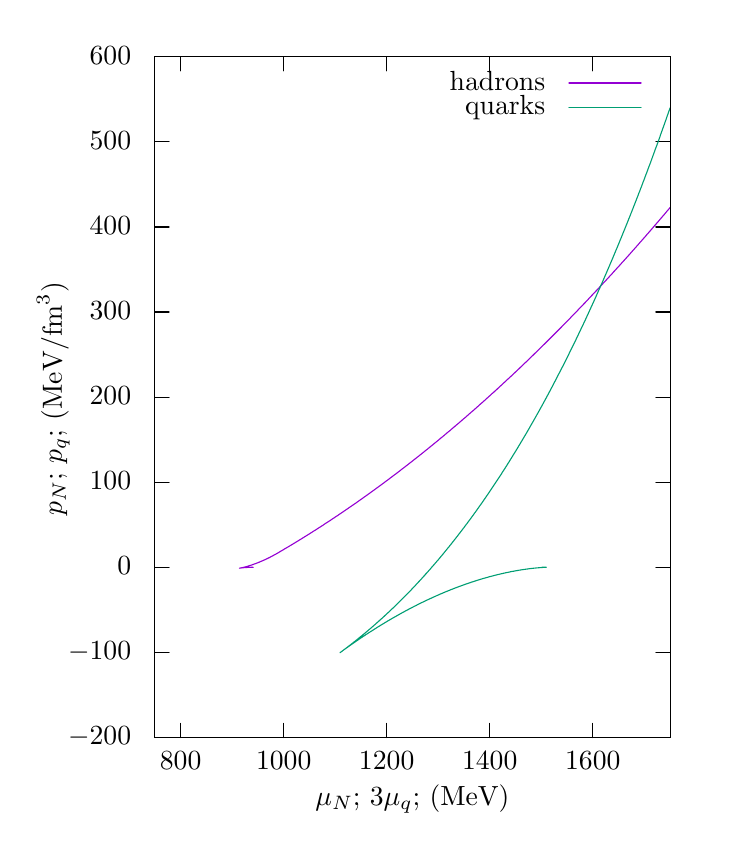
\begin{tikzpicture}[gnuplot]
%% generated with GNUPLOT 5.0p4 (Lua 5.2; terminal rev. 99, script rev. 100)
%% Thu Sep 29 16:33:18 2016
\path (0.000,0.000) rectangle (8.600,10.000);
\gpcolor{color=gp lt color border}
\gpsetlinetype{gp lt border}
\gpsetdashtype{gp dt solid}
\gpsetlinewidth{1.00}
\draw[gp path] (1.504,0.985)--(1.684,0.985);
\draw[gp path] (8.047,0.985)--(7.867,0.985);
\node[gp node right] at (1.320,0.985) {$-200$};
\draw[gp path] (1.504,2.066)--(1.684,2.066);
\draw[gp path] (8.047,2.066)--(7.867,2.066);
\node[gp node right] at (1.320,2.066) {$-100$};
\draw[gp path] (1.504,3.147)--(1.684,3.147);
\draw[gp path] (8.047,3.147)--(7.867,3.147);
\node[gp node right] at (1.320,3.147) {$0$};
\draw[gp path] (1.504,4.227)--(1.684,4.227);
\draw[gp path] (8.047,4.227)--(7.867,4.227);
\node[gp node right] at (1.320,4.227) {$100$};
\draw[gp path] (1.504,5.308)--(1.684,5.308);
\draw[gp path] (8.047,5.308)--(7.867,5.308);
\node[gp node right] at (1.320,5.308) {$200$};
\draw[gp path] (1.504,6.389)--(1.684,6.389);
\draw[gp path] (8.047,6.389)--(7.867,6.389);
\node[gp node right] at (1.320,6.389) {$300$};
\draw[gp path] (1.504,7.469)--(1.684,7.469);
\draw[gp path] (8.047,7.469)--(7.867,7.469);
\node[gp node right] at (1.320,7.469) {$400$};
\draw[gp path] (1.504,8.550)--(1.684,8.550);
\draw[gp path] (8.047,8.550)--(7.867,8.550);
\node[gp node right] at (1.320,8.550) {$500$};
\draw[gp path] (1.504,9.631)--(1.684,9.631);
\draw[gp path] (8.047,9.631)--(7.867,9.631);
\node[gp node right] at (1.320,9.631) {$600$};
\draw[gp path] (1.831,0.985)--(1.831,1.165);
\draw[gp path] (1.831,9.631)--(1.831,9.451);
\node[gp node center] at (1.831,0.677) {$800$};
\draw[gp path] (3.140,0.985)--(3.140,1.165);
\draw[gp path] (3.140,9.631)--(3.140,9.451);
\node[gp node center] at (3.140,0.677) {$1000$};
\draw[gp path] (4.448,0.985)--(4.448,1.165);
\draw[gp path] (4.448,9.631)--(4.448,9.451);
\node[gp node center] at (4.448,0.677) {$1200$};
\draw[gp path] (5.757,0.985)--(5.757,1.165);
\draw[gp path] (5.757,9.631)--(5.757,9.451);
\node[gp node center] at (5.757,0.677) {$1400$};
\draw[gp path] (7.066,0.985)--(7.066,1.165);
\draw[gp path] (7.066,9.631)--(7.066,9.451);
\node[gp node center] at (7.066,0.677) {$1600$};
\draw[gp path] (1.504,9.631)--(1.504,0.985)--(8.047,0.985)--(8.047,9.631)--cycle;
\node[gp node center,rotate=-270] at (0.246,5.308) {$p_N$; $p_q$; ($\rm{MeV}/\rm{fm}^3$)};
\node[gp node center] at (4.775,0.215) {$\mu_N$; $3\mu_q$; (MeV)};
\node[gp node right] at (6.579,9.297) {hadrons};
\gpcolor{rgb color={0.580,0.000,0.827}}
\draw[gp path] (6.763,9.297)--(7.679,9.297);
\draw[gp path] (2.728,3.146)--(2.736,3.146)--(2.745,3.147)--(2.753,3.147)--(2.722,3.146)%
  --(2.730,3.146)--(2.738,3.146)--(2.745,3.147)--(2.714,3.146)--(2.722,3.146)--(2.729,3.146)%
  --(2.736,3.146)--(2.744,3.147)--(2.713,3.146)--(2.720,3.146)--(2.727,3.146)--(2.734,3.147)%
  --(2.704,3.146)--(2.711,3.146)--(2.718,3.146)--(2.725,3.146)--(2.694,3.146)--(2.701,3.146)%
  --(2.709,3.146)--(2.716,3.146)--(2.685,3.145)--(2.692,3.146)--(2.699,3.146)--(2.706,3.146)%
  --(2.713,3.146)--(2.683,3.145)--(2.690,3.145)--(2.697,3.146)--(2.704,3.146)--(2.673,3.145)%
  --(2.680,3.145)--(2.688,3.145)--(2.695,3.146)--(2.664,3.144)--(2.671,3.145)--(2.679,3.145)%
  --(2.686,3.145)--(2.693,3.146)--(2.662,3.144)--(2.670,3.145)--(2.677,3.145)--(2.684,3.145)%
  --(2.653,3.144)--(2.661,3.144)--(2.668,3.144)--(2.675,3.145)--(2.645,3.143)--(2.652,3.144)%
  --(2.659,3.144)--(2.667,3.144)--(2.674,3.145)--(2.644,3.143)--(2.651,3.143)--(2.658,3.144)%
  --(2.665,3.144)--(2.635,3.142)--(2.643,3.143)--(2.650,3.143)--(2.657,3.144)--(2.627,3.142)%
  --(2.635,3.142)--(2.642,3.143)--(2.649,3.143)--(2.657,3.144)--(2.627,3.142)--(2.634,3.142)%
  --(2.642,3.143)--(2.649,3.143)--(2.619,3.141)--(2.627,3.142)--(2.634,3.142)--(2.641,3.143)%
  --(2.612,3.140)--(2.619,3.141)--(2.627,3.142)--(2.634,3.142)--(2.642,3.143)--(2.612,3.140)%
  --(2.619,3.141)--(2.627,3.142)--(2.635,3.142)--(2.605,3.139)--(2.613,3.140)--(2.620,3.141)%
  --(2.628,3.142)--(2.598,3.139)--(2.606,3.140)--(2.613,3.140)--(2.621,3.141)--(2.629,3.142)%
  --(2.599,3.139)--(2.607,3.140)--(2.615,3.140)--(2.622,3.141)--(2.593,3.138)--(2.601,3.139)%
  --(2.609,3.140)--(2.616,3.141)--(2.624,3.142)--(2.595,3.138)--(2.603,3.139)--(2.610,3.140)%
  --(2.618,3.141)--(2.589,3.137)--(2.597,3.138)--(2.605,3.139)--(2.612,3.140)--(2.620,3.141)%
  --(2.591,3.138)--(2.599,3.139)--(2.607,3.140)--(2.615,3.141)--(2.586,3.137)--(2.594,3.138)%
  --(2.602,3.139)--(2.610,3.140)--(2.581,3.136)--(2.589,3.137)--(2.597,3.138)--(2.605,3.139)%
  --(2.613,3.140)--(2.584,3.137)--(2.592,3.138)--(2.600,3.139)--(2.608,3.140)--(2.580,3.136)%
  --(2.588,3.137)--(2.596,3.138)--(2.604,3.139)--(2.612,3.140)--(2.583,3.136)--(2.591,3.137)%
  --(2.599,3.139)--(2.607,3.140)--(2.579,3.136)--(2.587,3.137)--(2.595,3.138)--(2.603,3.139)%
  --(2.612,3.141)--(2.583,3.136)--(2.592,3.137)--(2.600,3.139)--(2.608,3.140)--(2.580,3.136)%
  --(2.588,3.137)--(2.596,3.138)--(2.604,3.140)--(2.613,3.141)--(2.585,3.136)--(2.593,3.138)%
  --(2.601,3.139)--(2.609,3.141)--(2.582,3.136)--(2.590,3.137)--(2.598,3.139)--(2.606,3.140)%
  --(2.579,3.135)--(2.587,3.137)--(2.595,3.138)--(2.604,3.140)--(2.612,3.141)--(2.585,3.136)%
  --(2.593,3.138)--(2.601,3.139)--(2.609,3.141)--(2.582,3.136)--(2.591,3.137)--(2.599,3.139)%
  --(2.607,3.140)--(2.616,3.142)--(2.588,3.137)--(2.597,3.138)--(2.605,3.140)--(2.614,3.142)%
  --(2.587,3.136)--(2.595,3.138)--(2.603,3.140)--(2.612,3.141)--(2.620,3.143)--(2.593,3.138)%
  --(2.602,3.139)--(2.610,3.141)--(2.619,3.143)--(2.592,3.137)--(2.600,3.139)--(2.609,3.141)%
  --(2.617,3.143)--(2.626,3.144)--(2.599,3.139)--(2.608,3.141)--(2.616,3.142)--(2.625,3.144)%
  --(2.598,3.138)--(2.607,3.140)--(2.616,3.142)--(2.624,3.144)--(2.598,3.138)--(2.606,3.140)%
  --(2.615,3.142)--(2.624,3.144)--(2.632,3.146)--(2.606,3.140)--(2.615,3.142)--(2.623,3.144)%
  --(2.632,3.146)--(2.606,3.140)--(2.614,3.142)--(2.623,3.144)--(2.632,3.146)--(2.640,3.148)%
  --(2.614,3.142)--(2.623,3.144)--(2.632,3.146)--(2.641,3.148)--(2.615,3.142)--(2.623,3.144)%
  --(2.632,3.146)--(2.641,3.148)--(2.615,3.142)--(2.624,3.144)--(2.633,3.146)--(2.642,3.148)%
  --(2.650,3.151)--(2.625,3.144)--(2.633,3.146)--(2.642,3.149)--(2.651,3.151)--(2.626,3.144)%
  --(2.634,3.147)--(2.643,3.149)--(2.652,3.151)--(2.661,3.154)--(2.636,3.147)--(2.645,3.149)%
  --(2.653,3.152)--(2.662,3.154)--(2.637,3.147)--(2.646,3.150)--(2.655,3.152)--(2.664,3.154)%
  --(2.639,3.148)--(2.648,3.150)--(2.657,3.153)--(2.666,3.155)--(2.675,3.157)--(2.650,3.151)%
  --(2.659,3.153)--(2.668,3.156)--(2.676,3.158)--(2.652,3.151)--(2.661,3.154)--(2.670,3.156)%
  --(2.679,3.159)--(2.654,3.152)--(2.663,3.154)--(2.672,3.157)--(2.681,3.159)--(2.690,3.162)%
  --(2.674,3.157)--(2.683,3.160)--(2.675,3.158)--(2.684,3.161)--(2.677,3.158)--(2.686,3.161)%
  --(2.678,3.159)--(2.687,3.161)--(2.680,3.159)--(2.689,3.162)--(2.681,3.160)--(2.690,3.162)%
  --(2.683,3.160)--(2.692,3.163)--(2.685,3.161)--(2.694,3.163)--(2.703,3.166)--(2.696,3.164)%
  --(2.705,3.167)--(2.697,3.164)--(2.707,3.167)--(2.699,3.165)--(2.708,3.168)--(2.701,3.166)%
  --(2.710,3.169)--(2.703,3.166)--(2.712,3.169)--(2.705,3.167)--(2.714,3.170)--(2.707,3.168)%
  --(2.716,3.171)--(2.709,3.168)--(2.719,3.171)--(2.712,3.169)--(2.721,3.172)--(2.714,3.170)%
  --(2.723,3.173)--(2.716,3.170)--(2.725,3.173)--(2.735,3.177)--(2.728,3.174)--(2.737,3.177)%
  --(2.730,3.175)--(2.739,3.178)--(2.733,3.176)--(2.742,3.179)--(2.735,3.177)--(2.744,3.180)%
  --(2.738,3.178)--(2.747,3.181)--(2.740,3.179)--(2.750,3.182)--(2.743,3.180)--(2.752,3.183)%
  --(2.746,3.180)--(2.755,3.184)--(2.749,3.181)--(2.758,3.185)--(2.752,3.182)--(2.761,3.186)%
  --(2.755,3.184)--(2.764,3.187)--(2.757,3.185)--(2.767,3.188)--(2.761,3.186)--(2.770,3.189)%
  --(2.764,3.187)--(2.773,3.190)--(2.767,3.188)--(2.776,3.191)--(2.770,3.189)--(2.779,3.193)%
  --(2.773,3.190)--(2.783,3.194)--(2.777,3.192)--(2.786,3.195)--(2.780,3.193)--(2.789,3.196)%
  --(2.783,3.194)--(2.793,3.198)--(2.787,3.195)--(2.796,3.199)--(2.790,3.197)--(2.800,3.200)%
  --(2.794,3.198)--(2.803,3.202)--(2.798,3.200)--(2.807,3.203)--(2.801,3.201)--(2.796,3.199)%
  --(2.805,3.202)--(2.800,3.200)--(2.809,3.204)--(2.804,3.202)--(2.813,3.205)--(2.807,3.203)%
  --(2.817,3.207)--(2.811,3.205)--(2.821,3.209)--(2.816,3.206)--(2.825,3.210)--(2.820,3.208)%
  --(2.829,3.212)--(2.824,3.210)--(2.833,3.214)--(2.828,3.212)--(2.823,3.209)--(2.832,3.213)%
  --(2.827,3.211)--(2.837,3.215)--(2.832,3.213)--(2.841,3.217)--(2.836,3.215)--(2.846,3.219)%
  --(2.841,3.217)--(2.850,3.221)--(2.845,3.219)--(2.855,3.223)--(2.850,3.221)--(2.845,3.219)%
  --(2.855,3.223)--(2.850,3.221)--(2.859,3.225)--(2.855,3.223)--(2.864,3.227)--(2.860,3.225)%
  --(2.855,3.223)--(2.865,3.227)--(2.860,3.225)--(2.870,3.229)--(2.865,3.227)--(2.875,3.231)%
  --(2.870,3.229)--(2.880,3.234)--(2.876,3.232)--(2.871,3.230)--(2.881,3.234)--(2.877,3.232)%
  --(2.886,3.236)--(2.882,3.234)--(2.878,3.233)--(2.888,3.237)--(2.884,3.235)--(2.893,3.239)%
  --(2.889,3.238)--(2.899,3.242)--(2.895,3.240)--(2.891,3.238)--(2.901,3.243)--(2.897,3.241)%
  --(2.906,3.245)--(2.903,3.244)--(2.899,3.242)--(2.909,3.246)--(2.905,3.245)--(2.901,3.243)%
  --(2.911,3.248)--(2.908,3.246)--(2.917,3.250)--(2.914,3.249)--(2.910,3.247)--(2.920,3.252)%
  --(2.917,3.250)--(2.926,3.255)--(2.923,3.253)--(2.920,3.252)--(2.930,3.256)--(2.927,3.255)%
  --(2.924,3.254)--(2.933,3.258)--(2.930,3.257)--(2.928,3.255)--(2.937,3.260)--(2.934,3.259)%
  --(2.932,3.257)--(2.941,3.262)--(2.939,3.261)--(2.936,3.260)--(2.946,3.264)--(2.943,3.263)%
  --(2.941,3.262)--(2.950,3.267)--(2.948,3.265)--(2.946,3.264)--(2.956,3.269)--(2.950,3.267)%
  --(2.954,3.268)--(2.958,3.270)--(2.956,3.269)--(2.960,3.271)--(2.958,3.270)--(2.962,3.272)%
  --(2.960,3.271)--(2.964,3.273)--(2.963,3.273)--(2.967,3.275)--(2.971,3.277)--(2.969,3.276)%
  --(2.973,3.278)--(2.972,3.277)--(2.976,3.279)--(2.975,3.279)--(2.974,3.278)--(2.978,3.280)%
  --(2.977,3.280)--(2.981,3.282)--(2.985,3.284)--(2.984,3.284)--(2.984,3.283)--(2.988,3.286)%
  --(2.988,3.285)--(2.987,3.285)--(2.992,3.288)--(2.996,3.290)--(2.997,3.290)--(3.002,3.293)%
  --(3.003,3.294)--(3.004,3.294)--(3.005,3.295)--(3.006,3.295)--(3.007,3.296)--(3.008,3.296)%
  --(3.010,3.297)--(3.011,3.298)--(3.013,3.299)--(3.014,3.300)--(3.016,3.301)--(3.018,3.302)%
  --(3.020,3.303)--(3.018,3.302)--(3.020,3.303)--(3.023,3.304)--(3.022,3.304)--(3.024,3.305)%
  --(3.025,3.305)--(3.026,3.306)--(3.027,3.307)--(3.029,3.308)--(3.030,3.308)--(3.031,3.309)%
  --(3.032,3.310)--(3.034,3.310)--(3.034,3.311)--(3.036,3.312)--(3.038,3.313)--(3.040,3.314)%
  --(3.041,3.314)--(3.042,3.315)--(3.043,3.316)--(3.044,3.316)--(3.047,3.318)--(3.056,3.323)%
  --(3.066,3.329)--(3.075,3.334)--(3.084,3.340)--(3.094,3.345)--(3.103,3.351)--(3.113,3.356)%
  --(3.122,3.362)--(3.131,3.367)--(3.141,3.373)--(3.150,3.379)--(3.160,3.384)--(3.169,3.390)%
  --(3.178,3.395)--(3.188,3.401)--(3.197,3.406)--(3.207,3.412)--(3.216,3.418)--(3.225,3.423)%
  --(3.235,3.429)--(3.244,3.435)--(3.254,3.440)--(3.263,3.446)--(3.272,3.452)--(3.282,3.457)%
  --(3.291,3.463)--(3.300,3.469)--(3.310,3.474)--(3.319,3.480)--(3.329,3.486)--(3.338,3.492)%
  --(3.347,3.497)--(3.357,3.503)--(3.366,3.509)--(3.375,3.515)--(3.385,3.521)--(3.394,3.526)%
  --(3.403,3.532)--(3.413,3.538)--(3.422,3.544)--(3.432,3.550)--(3.441,3.555)--(3.450,3.561)%
  --(3.460,3.567)--(3.469,3.573)--(3.478,3.579)--(3.488,3.585)--(3.497,3.591)--(3.506,3.597)%
  --(3.516,3.603)--(3.525,3.609)--(3.534,3.614)--(3.544,3.620)--(3.553,3.626)--(3.562,3.632)%
  --(3.572,3.638)--(3.581,3.644)--(3.590,3.650)--(3.600,3.656)--(3.609,3.662)--(3.618,3.668)%
  --(3.628,3.674)--(3.637,3.680)--(3.646,3.686)--(3.655,3.693)--(3.665,3.699)--(3.674,3.705)%
  --(3.683,3.711)--(3.693,3.717)--(3.702,3.723)--(3.711,3.729)--(3.721,3.735)--(3.730,3.741)%
  --(3.739,3.747)--(3.749,3.754)--(3.758,3.760)--(3.767,3.766)--(3.776,3.772)--(3.786,3.778)%
  --(3.795,3.785)--(3.804,3.791)--(3.814,3.797)--(3.823,3.803)--(3.832,3.809)--(3.841,3.816)%
  --(3.851,3.822)--(3.860,3.828)--(3.869,3.834)--(3.879,3.841)--(3.888,3.847)--(3.897,3.853)%
  --(3.906,3.860)--(3.916,3.866)--(3.925,3.872)--(3.934,3.879)--(3.943,3.885)--(3.953,3.891)%
  --(3.962,3.898)--(3.971,3.904)--(3.981,3.911)--(3.990,3.917)--(3.999,3.923)--(4.008,3.930)%
  --(4.018,3.936)--(4.027,3.943)--(4.036,3.949)--(4.045,3.955)--(4.055,3.962)--(4.064,3.968)%
  --(4.073,3.975)--(4.082,3.981)--(4.092,3.988)--(4.101,3.994)--(4.110,4.001)--(4.119,4.007)%
  --(4.129,4.014)--(4.138,4.020)--(4.147,4.027)--(4.156,4.034)--(4.166,4.040)--(4.175,4.047)%
  --(4.184,4.053)--(4.193,4.060)--(4.203,4.067)--(4.212,4.073)--(4.221,4.080)--(4.230,4.086)%
  --(4.239,4.093)--(4.249,4.100)--(4.258,4.106)--(4.267,4.113)--(4.276,4.120)--(4.286,4.126)%
  --(4.295,4.133)--(4.304,4.140)--(4.313,4.147)--(4.322,4.153)--(4.332,4.160)--(4.341,4.167)%
  --(4.350,4.174)--(4.359,4.180)--(4.369,4.187)--(4.378,4.194)--(4.387,4.201)--(4.396,4.207)%
  --(4.405,4.214)--(4.415,4.221)--(4.424,4.228)--(4.433,4.235)--(4.442,4.242)--(4.451,4.248)%
  --(4.461,4.255)--(4.470,4.262)--(4.479,4.269)--(4.488,4.276)--(4.497,4.283)--(4.507,4.290)%
  --(4.516,4.297)--(4.525,4.304)--(4.534,4.311)--(4.543,4.318)--(4.553,4.325)--(4.562,4.331)%
  --(4.571,4.338)--(4.580,4.345)--(4.589,4.352)--(4.598,4.359)--(4.608,4.366)--(4.617,4.373)%
  --(4.626,4.381)--(4.635,4.388)--(4.644,4.395)--(4.653,4.402)--(4.663,4.409)--(4.672,4.416)%
  --(4.681,4.423)--(4.690,4.430)--(4.699,4.437)--(4.709,4.444)--(4.718,4.451)--(4.727,4.458)%
  --(4.736,4.466)--(4.745,4.473)--(4.754,4.480)--(4.764,4.487)--(4.773,4.494)--(4.782,4.502)%
  --(4.791,4.509)--(4.800,4.516)--(4.809,4.523)--(4.818,4.530)--(4.828,4.538)--(4.837,4.545)%
  --(4.846,4.552)--(4.855,4.559)--(4.864,4.567)--(4.873,4.574)--(4.883,4.581)--(4.892,4.589)%
  --(4.901,4.596)--(4.910,4.603)--(4.919,4.610)--(4.928,4.618)--(4.937,4.625)--(4.947,4.633)%
  --(4.956,4.640)--(4.965,4.647)--(4.974,4.655)--(4.983,4.662)--(4.992,4.669)--(5.001,4.677)%
  --(5.010,4.684)--(5.020,4.692)--(5.029,4.699)--(5.038,4.707)--(5.047,4.714)--(5.056,4.722)%
  --(5.065,4.729)--(5.074,4.736)--(5.084,4.744)--(5.093,4.751)--(5.102,4.759)--(5.111,4.767)%
  --(5.120,4.774)--(5.129,4.782)--(5.138,4.789)--(5.147,4.797)--(5.157,4.804)--(5.166,4.812)%
  --(5.175,4.819)--(5.184,4.827)--(5.193,4.835)--(5.202,4.842)--(5.211,4.850)--(5.220,4.858)%
  --(5.229,4.865)--(5.239,4.873)--(5.248,4.880)--(5.257,4.888)--(5.266,4.896)--(5.275,4.904)%
  --(5.284,4.911)--(5.293,4.919)--(5.302,4.927)--(5.311,4.934)--(5.320,4.942)--(5.330,4.950)%
  --(5.339,4.958)--(5.348,4.965)--(5.357,4.973)--(5.366,4.981)--(5.375,4.989)--(5.384,4.996)%
  --(5.393,5.004)--(5.402,5.012)--(5.411,5.020)--(5.420,5.028)--(5.430,5.036)--(5.439,5.043)%
  --(5.448,5.051)--(5.457,5.059)--(5.466,5.067)--(5.475,5.075)--(5.484,5.083)--(5.493,5.091)%
  --(5.502,5.099)--(5.511,5.107)--(5.520,5.115)--(5.530,5.123)--(5.539,5.130)--(5.548,5.138)%
  --(5.557,5.146)--(5.566,5.154)--(5.575,5.162)--(5.584,5.170)--(5.593,5.178)--(5.602,5.186)%
  --(5.611,5.194)--(5.620,5.203)--(5.629,5.211)--(5.638,5.219)--(5.647,5.227)--(5.657,5.235)%
  --(5.666,5.243)--(5.675,5.251)--(5.684,5.259)--(5.693,5.267)--(5.702,5.275)--(5.711,5.283)%
  --(5.720,5.292)--(5.729,5.300)--(5.738,5.308)--(5.747,5.316)--(5.756,5.324)--(5.765,5.332)%
  --(5.774,5.341)--(5.783,5.349)--(5.792,5.357)--(5.801,5.365)--(5.811,5.373)--(5.820,5.382)%
  --(5.829,5.390)--(5.838,5.398)--(5.847,5.406)--(5.856,5.415)--(5.865,5.423)--(5.874,5.431)%
  --(5.883,5.440)--(5.892,5.448)--(5.901,5.456)--(5.910,5.465)--(5.919,5.473)--(5.928,5.481)%
  --(5.937,5.490)--(5.946,5.498)--(5.955,5.506)--(5.964,5.515)--(5.973,5.523)--(5.982,5.532)%
  --(5.991,5.540)--(6.000,5.548)--(6.009,5.557)--(6.018,5.565)--(6.028,5.574)--(6.037,5.582)%
  --(6.046,5.591)--(6.055,5.599)--(6.064,5.608)--(6.073,5.616)--(6.082,5.625)--(6.091,5.633)%
  --(6.100,5.642)--(6.109,5.650)--(6.118,5.659)--(6.127,5.667)--(6.136,5.676)--(6.145,5.685)%
  --(6.154,5.693)--(6.163,5.702)--(6.172,5.710)--(6.181,5.719)--(6.190,5.728)--(6.199,5.736)%
  --(6.208,5.745)--(6.217,5.753)--(6.226,5.762)--(6.235,5.771)--(6.244,5.779)--(6.253,5.788)%
  --(6.262,5.797)--(6.271,5.805)--(6.280,5.814)--(6.289,5.823)--(6.298,5.832)--(6.307,5.840)%
  --(6.316,5.849)--(6.325,5.858)--(6.334,5.867)--(6.343,5.875)--(6.352,5.884)--(6.361,5.893)%
  --(6.370,5.902)--(6.379,5.911)--(6.388,5.919)--(6.397,5.928)--(6.406,5.937)--(6.415,5.946)%
  --(6.424,5.955)--(6.433,5.964)--(6.442,5.973)--(6.451,5.981)--(6.460,5.990)--(6.469,5.999)%
  --(6.478,6.008)--(6.487,6.017)--(6.496,6.026)--(6.505,6.035)--(6.514,6.044)--(6.523,6.053)%
  --(6.532,6.062)--(6.541,6.071)--(6.550,6.080)--(6.559,6.089)--(6.568,6.098)--(6.577,6.107)%
  --(6.586,6.116)--(6.595,6.125)--(6.604,6.134)--(6.613,6.143)--(6.622,6.152)--(6.631,6.161)%
  --(6.640,6.170)--(6.649,6.179)--(6.658,6.188)--(6.667,6.197)--(6.676,6.207)--(6.685,6.216)%
  --(6.694,6.225)--(6.703,6.234)--(6.712,6.243)--(6.721,6.252)--(6.730,6.261)--(6.739,6.271)%
  --(6.748,6.280)--(6.757,6.289)--(6.766,6.298)--(6.775,6.307)--(6.784,6.317)--(6.792,6.326)%
  --(6.801,6.335)--(6.810,6.344)--(6.819,6.354)--(6.828,6.363)--(6.837,6.372)--(6.846,6.381)%
  --(6.855,6.391)--(6.864,6.400)--(6.873,6.409)--(6.882,6.419)--(6.891,6.428)--(6.900,6.437)%
  --(6.909,6.447)--(6.918,6.456)--(6.927,6.465)--(6.936,6.475)--(6.945,6.484)--(6.954,6.494)%
  --(6.963,6.503)--(6.972,6.512)--(6.981,6.522)--(6.990,6.531)--(6.999,6.541)--(7.008,6.550)%
  --(7.016,6.560)--(7.025,6.569)--(7.034,6.579)--(7.043,6.588)--(7.052,6.598)--(7.061,6.607)%
  --(7.070,6.617)--(7.079,6.626)--(7.088,6.636)--(7.097,6.645)--(7.106,6.655)--(7.115,6.664)%
  --(7.124,6.674)--(7.133,6.683)--(7.142,6.693)--(7.151,6.703)--(7.160,6.712)--(7.169,6.722)%
  --(7.177,6.732)--(7.186,6.741)--(7.195,6.751)--(7.204,6.760)--(7.213,6.770)--(7.222,6.780)%
  --(7.231,6.789)--(7.240,6.799)--(7.249,6.809)--(7.258,6.819)--(7.267,6.828)--(7.276,6.838)%
  --(7.285,6.848)--(7.294,6.857)--(7.303,6.867)--(7.312,6.877)--(7.320,6.887)--(7.329,6.897)%
  --(7.338,6.906)--(7.347,6.916)--(7.356,6.926)--(7.365,6.936)--(7.374,6.946)--(7.383,6.955)%
  --(7.392,6.965)--(7.401,6.975)--(7.410,6.985)--(7.419,6.995)--(7.428,7.005)--(7.436,7.015)%
  --(7.445,7.025)--(7.454,7.034)--(7.463,7.044)--(7.472,7.054)--(7.481,7.064)--(7.490,7.074)%
  --(7.499,7.084)--(7.508,7.094)--(7.517,7.104)--(7.526,7.114)--(7.535,7.124)--(7.544,7.134)%
  --(7.552,7.144)--(7.561,7.154)--(7.570,7.164)--(7.579,7.174)--(7.588,7.184)--(7.597,7.194)%
  --(7.606,7.204)--(7.615,7.214)--(7.624,7.225)--(7.633,7.235)--(7.642,7.245)--(7.650,7.255)%
  --(7.659,7.265)--(7.668,7.275)--(7.677,7.285)--(7.686,7.295)--(7.695,7.306)--(7.704,7.316)%
  --(7.713,7.326)--(7.722,7.336)--(7.731,7.346)--(7.740,7.356)--(7.748,7.367)--(7.757,7.377)%
  --(7.766,7.387)--(7.775,7.397)--(7.784,7.408)--(7.793,7.418)--(7.802,7.428)--(7.811,7.438)%
  --(7.820,7.449)--(7.828,7.459)--(7.837,7.469)--(7.846,7.480)--(7.855,7.490)--(7.864,7.500)%
  --(7.873,7.511)--(7.882,7.521)--(7.891,7.531)--(7.900,7.542)--(7.909,7.552)--(7.917,7.562)%
  --(7.926,7.573)--(7.935,7.583)--(7.944,7.594)--(7.953,7.604)--(7.962,7.614)--(7.971,7.625)%
  --(7.980,7.635)--(7.989,7.646)--(7.997,7.656)--(8.006,7.667)--(8.015,7.677)--(8.024,7.688)%
  --(8.033,7.698)--(8.042,7.709)--(8.047,7.715);
\gpcolor{color=gp lt color border}
\node[gp node right] at (6.579,8.989) {quarks};
\gpcolor{rgb color={0.000,0.620,0.451}}
\draw[gp path] (6.763,8.989)--(7.679,8.989);
\draw[gp path] (6.423,3.147)--(6.445,3.147)--(6.457,3.147)--(6.465,3.147)--(6.470,3.147)%
  --(6.473,3.147)--(6.475,3.147)--(6.476,3.147)--(6.475,3.147)--(6.474,3.147)--(6.472,3.147)%
  --(6.470,3.147)--(6.467,3.147)--(6.463,3.146)--(6.460,3.146)--(6.455,3.146)--(6.451,3.146)%
  --(6.446,3.146)--(6.440,3.145)--(6.435,3.145)--(6.429,3.145)--(6.423,3.144)--(6.417,3.144)%
  --(6.410,3.144)--(6.404,3.143)--(6.397,3.143)--(6.390,3.142)--(6.383,3.141)--(6.376,3.141)%
  --(6.368,3.140)--(6.361,3.140)--(6.353,3.139)--(6.345,3.138)--(6.337,3.137)--(6.329,3.137)%
  --(6.321,3.136)--(6.313,3.135)--(6.304,3.134)--(6.296,3.133)--(6.287,3.132)--(6.279,3.131)%
  --(6.270,3.130)--(6.261,3.129)--(6.252,3.128)--(6.243,3.126)--(6.234,3.125)--(6.225,3.124)%
  --(6.216,3.123)--(6.207,3.121)--(6.197,3.120)--(6.188,3.119)--(6.179,3.117)--(6.169,3.116)%
  --(6.159,3.114)--(6.150,3.113)--(6.140,3.111)--(6.130,3.110)--(6.121,3.108)--(6.111,3.106)%
  --(6.101,3.105)--(6.091,3.103)--(6.081,3.101)--(6.071,3.099)--(6.061,3.097)--(6.051,3.096)%
  --(6.041,3.094)--(6.030,3.092)--(6.020,3.090)--(6.010,3.087)--(6.000,3.085)--(5.989,3.083)%
  --(5.979,3.081)--(5.968,3.079)--(5.958,3.077)--(5.947,3.074)--(5.937,3.072)--(5.926,3.070)%
  --(5.916,3.067)--(5.905,3.065)--(5.894,3.062)--(5.884,3.060)--(5.873,3.057)--(5.862,3.055)%
  --(5.851,3.052)--(5.841,3.049)--(5.830,3.047)--(5.819,3.044)--(5.808,3.041)--(5.797,3.038)%
  --(5.786,3.035)--(5.775,3.032)--(5.764,3.030)--(5.753,3.027)--(5.742,3.024)--(5.731,3.020)%
  --(5.720,3.017)--(5.709,3.014)--(5.698,3.011)--(5.687,3.008)--(5.675,3.005)--(5.664,3.001)%
  --(5.653,2.998)--(5.642,2.995)--(5.630,2.991)--(5.619,2.988)--(5.608,2.984)--(5.596,2.981)%
  --(5.585,2.977)--(5.574,2.973)--(5.562,2.970)--(5.551,2.966)--(5.539,2.962)--(5.528,2.959)%
  --(5.517,2.955)--(5.505,2.951)--(5.494,2.947)--(5.482,2.943)--(5.471,2.939)--(5.459,2.935)%
  --(5.447,2.931)--(5.436,2.927)--(5.424,2.923)--(5.413,2.919)--(5.401,2.914)--(5.389,2.910)%
  --(5.378,2.906)--(5.366,2.902)--(5.354,2.897)--(5.343,2.893)--(5.331,2.888)--(5.319,2.884)%
  --(5.307,2.879)--(5.296,2.875)--(5.284,2.870)--(5.272,2.866)--(5.260,2.861)--(5.249,2.856)%
  --(5.237,2.851)--(5.225,2.847)--(5.213,2.842)--(5.201,2.837)--(5.189,2.832)--(5.177,2.827)%
  --(5.166,2.822)--(5.154,2.817)--(5.142,2.812)--(5.130,2.807)--(5.118,2.801)--(5.106,2.796)%
  --(5.094,2.791)--(5.082,2.786)--(5.070,2.780)--(5.058,2.775)--(5.046,2.770)--(5.034,2.764)%
  --(5.022,2.759)--(5.010,2.753)--(4.998,2.748)--(4.986,2.742)--(4.973,2.736)--(4.961,2.731)%
  --(4.949,2.725)--(4.937,2.719)--(4.925,2.713)--(4.913,2.707)--(4.901,2.702)--(4.889,2.696)%
  --(4.877,2.690)--(4.864,2.684)--(4.852,2.678)--(4.840,2.672)--(4.828,2.665)--(4.816,2.659)%
  --(4.803,2.653)--(4.791,2.647)--(4.779,2.640)--(4.767,2.634)--(4.754,2.628)--(4.742,2.621)%
  --(4.730,2.615)--(4.718,2.608)--(4.705,2.602)--(4.693,2.595)--(4.681,2.589)--(4.669,2.582)%
  --(4.656,2.575)--(4.644,2.569)--(4.632,2.562)--(4.619,2.555)--(4.607,2.548)--(4.595,2.541)%
  --(4.582,2.534)--(4.570,2.527)--(4.558,2.520)--(4.545,2.513)--(4.533,2.506)--(4.520,2.499)%
  --(4.508,2.492)--(4.496,2.484)--(4.483,2.477)--(4.471,2.470)--(4.458,2.463)--(4.446,2.455)%
  --(4.433,2.448)--(4.421,2.440)--(4.409,2.433)--(4.396,2.425)--(4.384,2.418)--(4.371,2.410)%
  --(4.359,2.402)--(4.346,2.395)--(4.334,2.387)--(4.321,2.379)--(4.309,2.371)--(4.296,2.363)%
  --(4.284,2.355)--(4.271,2.347)--(4.259,2.339)--(4.246,2.331)--(4.233,2.323)--(4.221,2.315)%
  --(4.208,2.307)--(4.196,2.299)--(4.183,2.291)--(4.171,2.282)--(4.158,2.274)--(4.146,2.266)%
  --(4.133,2.257)--(4.120,2.249)--(4.108,2.240)--(4.095,2.232)--(4.083,2.223)--(4.070,2.215)%
  --(4.057,2.206)--(4.045,2.197)--(4.032,2.188)--(4.019,2.180)--(4.007,2.171)--(3.994,2.162)%
  --(3.981,2.153)--(3.969,2.144)--(3.956,2.135)--(3.943,2.126)--(3.931,2.117)--(3.918,2.108)%
  --(3.905,2.099)--(3.893,2.090)--(3.880,2.080)--(3.867,2.071)--(3.855,2.062)--(3.864,2.069)%
  --(3.874,2.076)--(3.884,2.083)--(3.893,2.090)--(3.903,2.098)--(3.912,2.105)--(3.922,2.112)%
  --(3.931,2.119)--(3.941,2.126)--(3.950,2.133)--(3.960,2.141)--(3.969,2.148)--(3.979,2.155)%
  --(3.988,2.162)--(3.997,2.170)--(4.007,2.177)--(4.016,2.184)--(4.025,2.191)--(4.034,2.199)%
  --(4.044,2.206)--(4.053,2.213)--(4.062,2.221)--(4.071,2.228)--(4.080,2.235)--(4.089,2.243)%
  --(4.098,2.250)--(4.107,2.257)--(4.116,2.265)--(4.126,2.272)--(4.135,2.280)--(4.143,2.287)%
  --(4.152,2.294)--(4.161,2.302)--(4.170,2.309)--(4.179,2.317)--(4.188,2.324)--(4.197,2.331)%
  --(4.206,2.339)--(4.215,2.346)--(4.223,2.354)--(4.232,2.361)--(4.241,2.369)--(4.250,2.376)%
  --(4.258,2.384)--(4.267,2.391)--(4.276,2.399)--(4.284,2.406)--(4.293,2.414)--(4.302,2.421)%
  --(4.310,2.429)--(4.319,2.437)--(4.327,2.444)--(4.336,2.452)--(4.344,2.459)--(4.353,2.467)%
  --(4.361,2.475)--(4.370,2.482)--(4.378,2.490)--(4.387,2.497)--(4.395,2.505)--(4.403,2.513)%
  --(4.412,2.520)--(4.420,2.528)--(4.428,2.536)--(4.437,2.543)--(4.445,2.551)--(4.453,2.559)%
  --(4.462,2.567)--(4.470,2.574)--(4.478,2.582)--(4.486,2.590)--(4.495,2.597)--(4.503,2.605)%
  --(4.511,2.613)--(4.519,2.621)--(4.527,2.628)--(4.535,2.636)--(4.543,2.644)--(4.551,2.652)%
  --(4.559,2.660)--(4.568,2.667)--(4.576,2.675)--(4.584,2.683)--(4.592,2.691)--(4.600,2.699)%
  --(4.608,2.707)--(4.615,2.714)--(4.623,2.722)--(4.631,2.730)--(4.639,2.738)--(4.647,2.746)%
  --(4.655,2.754)--(4.663,2.762)--(4.671,2.770)--(4.678,2.778)--(4.686,2.786)--(4.694,2.793)%
  --(4.702,2.801)--(4.710,2.809)--(4.717,2.817)--(4.725,2.825)--(4.733,2.833)--(4.741,2.841)%
  --(4.748,2.849)--(4.756,2.857)--(4.764,2.865)--(4.771,2.873)--(4.779,2.881)--(4.787,2.889)%
  --(4.794,2.897)--(4.802,2.905)--(4.809,2.913)--(4.817,2.921)--(4.824,2.930)--(4.832,2.938)%
  --(4.839,2.946)--(4.847,2.954)--(4.854,2.962)--(4.862,2.970)--(4.869,2.978)--(4.877,2.986)%
  --(4.884,2.994)--(4.892,3.002)--(4.899,3.011)--(4.907,3.019)--(4.914,3.027)--(4.921,3.035)%
  --(4.929,3.043)--(4.936,3.051)--(4.943,3.060)--(4.951,3.068)--(4.958,3.076)--(4.965,3.084)%
  --(4.973,3.092)--(4.980,3.101)--(4.987,3.109)--(4.994,3.117)--(5.002,3.125)--(5.009,3.134)%
  --(5.016,3.142)--(5.023,3.150)--(5.030,3.158)--(5.038,3.167)--(5.045,3.175)--(5.052,3.183)%
  --(5.059,3.191)--(5.066,3.200)--(5.073,3.208)--(5.080,3.216)--(5.087,3.225)--(5.095,3.233)%
  --(5.102,3.241)--(5.109,3.250)--(5.116,3.258)--(5.123,3.266)--(5.130,3.275)--(5.137,3.283)%
  --(5.144,3.291)--(5.151,3.300)--(5.158,3.308)--(5.165,3.317)--(5.172,3.325)--(5.179,3.333)%
  --(5.185,3.342)--(5.192,3.350)--(5.199,3.359)--(5.206,3.367)--(5.213,3.376)--(5.220,3.384)%
  --(5.227,3.393)--(5.234,3.401)--(5.241,3.409)--(5.247,3.418)--(5.254,3.426)--(5.261,3.435)%
  --(5.268,3.443)--(5.275,3.452)--(5.281,3.460)--(5.288,3.469)--(5.295,3.477)--(5.302,3.486)%
  --(5.308,3.495)--(5.315,3.503)--(5.322,3.512)--(5.328,3.520)--(5.335,3.529)--(5.342,3.537)%
  --(5.349,3.546)--(5.355,3.555)--(5.362,3.563)--(5.368,3.572)--(5.375,3.580)--(5.382,3.589)%
  --(5.388,3.598)--(5.395,3.606)--(5.402,3.615)--(5.408,3.623)--(5.415,3.632)--(5.421,3.641)%
  --(5.428,3.649)--(5.434,3.658)--(5.441,3.667)--(5.447,3.675)--(5.454,3.684)--(5.460,3.693)%
  --(5.467,3.701)--(5.473,3.710)--(5.480,3.719)--(5.486,3.728)--(5.493,3.736)--(5.499,3.745)%
  --(5.506,3.754)--(5.512,3.762)--(5.519,3.771)--(5.525,3.780)--(5.531,3.789)--(5.538,3.797)%
  --(5.544,3.806)--(5.551,3.815)--(5.557,3.824)--(5.563,3.833)--(5.570,3.841)--(5.576,3.850)%
  --(5.582,3.859)--(5.589,3.868)--(5.595,3.877)--(5.601,3.885)--(5.607,3.894)--(5.614,3.903)%
  --(5.620,3.912)--(5.626,3.921)--(5.633,3.930)--(5.639,3.939)--(5.645,3.947)--(5.651,3.956)%
  --(5.658,3.965)--(5.664,3.974)--(5.670,3.983)--(5.676,3.992)--(5.682,4.001)--(5.688,4.010)%
  --(5.695,4.019)--(5.701,4.027)--(5.707,4.036)--(5.713,4.045)--(5.719,4.054)--(5.725,4.063)%
  --(5.732,4.072)--(5.738,4.081)--(5.744,4.090)--(5.750,4.099)--(5.756,4.108)--(5.762,4.117)%
  --(5.768,4.126)--(5.774,4.135)--(5.780,4.144)--(5.786,4.153)--(5.792,4.162)--(5.798,4.171)%
  --(5.804,4.180)--(5.810,4.189)--(5.816,4.198)--(5.822,4.207)--(5.828,4.216)--(5.834,4.225)%
  --(5.840,4.234)--(5.846,4.243)--(5.852,4.253)--(5.858,4.262)--(5.864,4.271)--(5.870,4.280)%
  --(5.876,4.289)--(5.882,4.298)--(5.888,4.307)--(5.894,4.316)--(5.900,4.325)--(5.906,4.334)%
  --(5.912,4.344)--(5.917,4.353)--(5.923,4.362)--(5.929,4.371)--(5.935,4.380)--(5.941,4.389)%
  --(5.947,4.398)--(5.953,4.408)--(5.958,4.417)--(5.964,4.426)--(5.970,4.435)--(5.976,4.444)%
  --(5.982,4.454)--(5.987,4.463)--(5.993,4.472)--(5.999,4.481)--(6.005,4.490)--(6.011,4.500)%
  --(6.016,4.509)--(6.022,4.518)--(6.028,4.527)--(6.034,4.537)--(6.039,4.546)--(6.045,4.555)%
  --(6.051,4.564)--(6.056,4.574)--(6.062,4.583)--(6.068,4.592)--(6.074,4.602)--(6.079,4.611)%
  --(6.085,4.620)--(6.091,4.629)--(6.096,4.639)--(6.102,4.648)--(6.108,4.657)--(6.113,4.667)%
  --(6.119,4.676)--(6.124,4.685)--(6.130,4.695)--(6.136,4.704)--(6.141,4.713)--(6.147,4.723)%
  --(6.152,4.732)--(6.158,4.742)--(6.164,4.751)--(6.169,4.760)--(6.175,4.770)--(6.180,4.779)%
  --(6.186,4.788)--(6.191,4.798)--(6.197,4.807)--(6.203,4.817)--(6.208,4.826)--(6.214,4.836)%
  --(6.219,4.845)--(6.225,4.854)--(6.230,4.864)--(6.236,4.873)--(6.241,4.883)--(6.247,4.892)%
  --(6.252,4.902)--(6.258,4.911)--(6.263,4.921)--(6.268,4.930)--(6.274,4.940)--(6.279,4.949)%
  --(6.285,4.959)--(6.290,4.968)--(6.296,4.978)--(6.301,4.987)--(6.307,4.997)--(6.312,5.006)%
  --(6.317,5.016)--(6.323,5.025)--(6.328,5.035)--(6.334,5.044)--(6.339,5.054)--(6.344,5.063)%
  --(6.350,5.073)--(6.355,5.083)--(6.360,5.092)--(6.366,5.102)--(6.371,5.111)--(6.376,5.121)%
  --(6.382,5.130)--(6.387,5.140)--(6.392,5.150)--(6.398,5.159)--(6.403,5.169)--(6.408,5.178)%
  --(6.414,5.188)--(6.419,5.198)--(6.424,5.207)--(6.430,5.217)--(6.435,5.227)--(6.440,5.236)%
  --(6.445,5.246)--(6.451,5.256)--(6.456,5.265)--(6.461,5.275)--(6.466,5.285)--(6.472,5.294)%
  --(6.477,5.304)--(6.482,5.314)--(6.487,5.323)--(6.493,5.333)--(6.498,5.343)--(6.503,5.352)%
  --(6.508,5.362)--(6.513,5.372)--(6.519,5.382)--(6.524,5.391)--(6.529,5.401)--(6.534,5.411)%
  --(6.539,5.421)--(6.544,5.430)--(6.550,5.440)--(6.555,5.450)--(6.560,5.460)--(6.565,5.469)%
  --(6.570,5.479)--(6.575,5.489)--(6.580,5.499)--(6.586,5.509)--(6.591,5.518)--(6.596,5.528)%
  --(6.601,5.538)--(6.606,5.548)--(6.611,5.558)--(6.616,5.567)--(6.621,5.577)--(6.626,5.587)%
  --(6.631,5.597)--(6.636,5.607)--(6.642,5.617)--(6.647,5.626)--(6.652,5.636)--(6.657,5.646)%
  --(6.662,5.656)--(6.667,5.666)--(6.672,5.676)--(6.677,5.686)--(6.682,5.695)--(6.687,5.705)%
  --(6.692,5.715)--(6.697,5.725)--(6.702,5.735)--(6.707,5.745)--(6.712,5.755)--(6.717,5.765)%
  --(6.722,5.775)--(6.727,5.785)--(6.732,5.795)--(6.737,5.805)--(6.742,5.814)--(6.747,5.824)%
  --(6.752,5.834)--(6.757,5.844)--(6.762,5.854)--(6.766,5.864)--(6.771,5.874)--(6.776,5.884)%
  --(6.781,5.894)--(6.786,5.904)--(6.791,5.914)--(6.796,5.924)--(6.801,5.934)--(6.806,5.944)%
  --(6.811,5.954)--(6.816,5.964)--(6.821,5.974)--(6.825,5.984)--(6.830,5.994)--(6.835,6.004)%
  --(6.840,6.014)--(6.845,6.024)--(6.850,6.034)--(6.855,6.045)--(6.859,6.055)--(6.864,6.065)%
  --(6.869,6.075)--(6.874,6.085)--(6.879,6.095)--(6.884,6.105)--(6.888,6.115)--(6.893,6.125)%
  --(6.898,6.135)--(6.903,6.145)--(6.908,6.155)--(6.913,6.166)--(6.917,6.176)--(6.922,6.186)%
  --(6.927,6.196)--(6.932,6.206)--(6.936,6.216)--(6.941,6.226)--(6.946,6.236)--(6.951,6.247)%
  --(6.956,6.257)--(6.960,6.267)--(6.965,6.277)--(6.970,6.287)--(6.975,6.297)--(6.979,6.308)%
  --(6.984,6.318)--(6.989,6.328)--(6.993,6.338)--(6.998,6.348)--(7.003,6.359)--(7.008,6.369)%
  --(7.012,6.379)--(7.017,6.389)--(7.022,6.399)--(7.026,6.410)--(7.031,6.420)--(7.036,6.430)%
  --(7.040,6.440)--(7.045,6.451)--(7.050,6.461)--(7.054,6.471)--(7.059,6.481)--(7.064,6.492)%
  --(7.068,6.502)--(7.073,6.512)--(7.078,6.522)--(7.082,6.533)--(7.087,6.543)--(7.092,6.553)%
  --(7.096,6.564)--(7.101,6.574)--(7.106,6.584)--(7.110,6.594)--(7.115,6.605)--(7.119,6.615)%
  --(7.124,6.625)--(7.129,6.636)--(7.133,6.646)--(7.138,6.656)--(7.142,6.667)--(7.147,6.677)%
  --(7.152,6.687)--(7.156,6.698)--(7.161,6.708)--(7.165,6.719)--(7.170,6.729)--(7.175,6.739)%
  --(7.179,6.750)--(7.184,6.760)--(7.188,6.770)--(7.193,6.781)--(7.197,6.791)--(7.202,6.802)%
  --(7.206,6.812)--(7.211,6.822)--(7.215,6.833)--(7.220,6.843)--(7.224,6.854)--(7.229,6.864)%
  --(7.234,6.874)--(7.238,6.885)--(7.243,6.895)--(7.247,6.906)--(7.252,6.916)--(7.256,6.927)%
  --(7.261,6.937)--(7.265,6.948)--(7.270,6.958)--(7.274,6.968)--(7.278,6.979)--(7.283,6.989)%
  --(7.287,7.000)--(7.292,7.010)--(7.296,7.021)--(7.301,7.031)--(7.305,7.042)--(7.310,7.052)%
  --(7.314,7.063)--(7.319,7.073)--(7.323,7.084)--(7.327,7.094)--(7.332,7.105)--(7.336,7.115)%
  --(7.341,7.126)--(7.345,7.137)--(7.350,7.147)--(7.354,7.158)--(7.358,7.168)--(7.363,7.179)%
  --(7.367,7.189)--(7.372,7.200)--(7.376,7.210)--(7.380,7.221)--(7.385,7.232)--(7.389,7.242)%
  --(7.394,7.253)--(7.398,7.263)--(7.402,7.274)--(7.407,7.285)--(7.411,7.295)--(7.415,7.306)%
  --(7.420,7.316)--(7.424,7.327)--(7.429,7.338)--(7.433,7.348)--(7.437,7.359)--(7.442,7.369)%
  --(7.446,7.380)--(7.450,7.391)--(7.455,7.401)--(7.459,7.412)--(7.463,7.423)--(7.468,7.433)%
  --(7.472,7.444)--(7.476,7.455)--(7.480,7.465)--(7.485,7.476)--(7.489,7.487)--(7.493,7.497)%
  --(7.498,7.508)--(7.502,7.519)--(7.506,7.529)--(7.511,7.540)--(7.515,7.551)--(7.519,7.562)%
  --(7.523,7.572)--(7.528,7.583)--(7.532,7.594)--(7.536,7.604)--(7.541,7.615)--(7.545,7.626)%
  --(7.549,7.637)--(7.553,7.647)--(7.558,7.658)--(7.562,7.669)--(7.566,7.680)--(7.570,7.690)%
  --(7.575,7.701)--(7.579,7.712)--(7.583,7.723)--(7.587,7.733)--(7.591,7.744)--(7.596,7.755)%
  --(7.600,7.766)--(7.604,7.777)--(7.608,7.787)--(7.613,7.798)--(7.617,7.809)--(7.621,7.820)%
  --(7.625,7.831)--(7.629,7.841)--(7.634,7.852)--(7.638,7.863)--(7.642,7.874)--(7.646,7.885)%
  --(7.650,7.896)--(7.654,7.906)--(7.659,7.917)--(7.663,7.928)--(7.667,7.939)--(7.671,7.950)%
  --(7.675,7.961)--(7.679,7.971)--(7.684,7.982)--(7.688,7.993)--(7.692,8.004)--(7.696,8.015)%
  --(7.700,8.026)--(7.704,8.037)--(7.708,8.048)--(7.713,8.059)--(7.717,8.069)--(7.721,8.080)%
  --(7.725,8.091)--(7.729,8.102)--(7.733,8.113)--(7.737,8.124)--(7.741,8.135)--(7.746,8.146)%
  --(7.750,8.157)--(7.754,8.168)--(7.758,8.179)--(7.762,8.190)--(7.766,8.201)--(7.770,8.212)%
  --(7.774,8.222)--(7.778,8.233)--(7.782,8.244)--(7.787,8.255)--(7.791,8.266)--(7.795,8.277)%
  --(7.799,8.288)--(7.803,8.299)--(7.807,8.310)--(7.811,8.321)--(7.815,8.332)--(7.819,8.343)%
  --(7.823,8.354)--(7.827,8.365)--(7.831,8.376)--(7.835,8.387)--(7.839,8.398)--(7.843,8.409)%
  --(7.847,8.420)--(7.851,8.431)--(7.855,8.442)--(7.859,8.453)--(7.863,8.465)--(7.867,8.476)%
  --(7.872,8.487)--(7.876,8.498)--(7.880,8.509)--(7.884,8.520)--(7.888,8.531)--(7.892,8.542)%
  --(7.896,8.553)--(7.900,8.564)--(7.904,8.575)--(7.908,8.586)--(7.912,8.597)--(7.916,8.608)%
  --(7.920,8.620)--(7.923,8.631)--(7.927,8.642)--(7.931,8.653)--(7.935,8.664)--(7.939,8.675)%
  --(7.943,8.686)--(7.947,8.697)--(7.951,8.709)--(7.955,8.720)--(7.959,8.731)--(7.963,8.742)%
  --(7.967,8.753)--(7.971,8.764)--(7.975,8.775)--(7.979,8.787)--(7.983,8.798)--(7.987,8.809)%
  --(7.991,8.820)--(7.995,8.831)--(7.999,8.842)--(8.003,8.854)--(8.006,8.865)--(8.010,8.876)%
  --(8.014,8.887)--(8.018,8.898)--(8.022,8.910)--(8.026,8.921)--(8.030,8.932)--(8.034,8.943)%
  --(8.038,8.954)--(8.042,8.966)--(8.046,8.977)--(8.047,8.981);
\gpcolor{color=gp lt color border}
\draw[gp path] (1.504,9.631)--(1.504,0.985)--(8.047,0.985)--(8.047,9.631)--cycle;
%% coordinates of the plot area
\gpdefrectangularnode{gp plot 1}{\pgfpoint{1.504cm}{0.985cm}}{\pgfpoint{8.047cm}{9.631cm}}
\end{tikzpicture}
%% gnuplot variables

	\caption{Buballa\_3-eNJL1OmegaRho1}
\end{figure}
\begin{figure}
	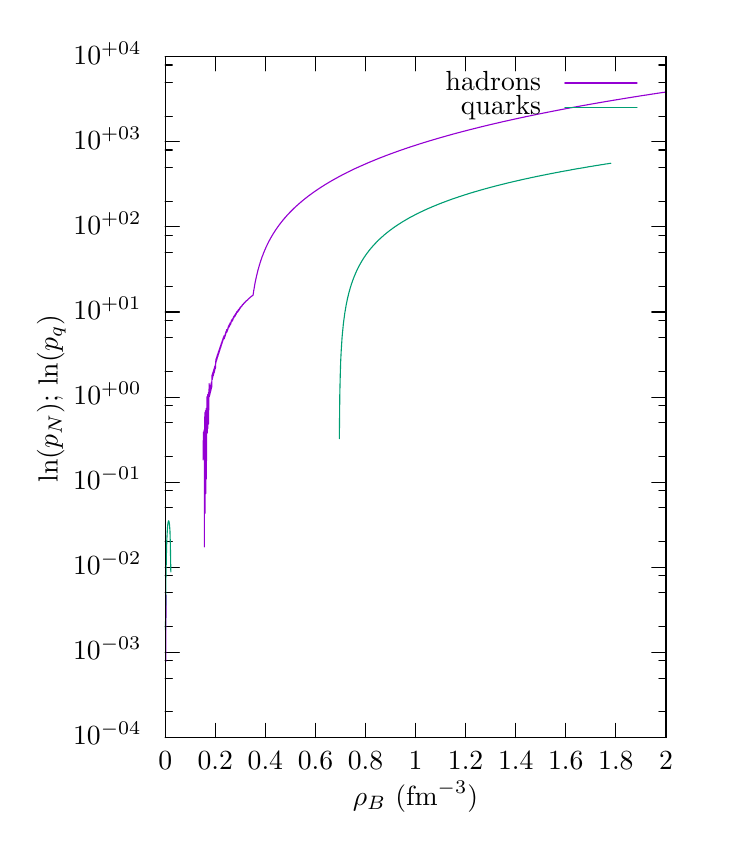
\begin{tikzpicture}[gnuplot]
%% generated with GNUPLOT 5.0p4 (Lua 5.2; terminal rev. 99, script rev. 100)
%% Thu Sep 29 16:33:18 2016
\path (0.000,0.000) rectangle (8.600,10.000);
\gpcolor{color=gp lt color border}
\gpsetlinetype{gp lt border}
\gpsetdashtype{gp dt solid}
\gpsetlinewidth{1.00}
\draw[gp path] (1.688,0.985)--(1.868,0.985);
\draw[gp path] (8.047,0.985)--(7.867,0.985);
\node[gp node right] at (1.504,0.985) {$10^{-04}$};
\draw[gp path] (1.688,1.310)--(1.778,1.310);
\draw[gp path] (8.047,1.310)--(7.957,1.310);
\draw[gp path] (1.688,1.740)--(1.778,1.740);
\draw[gp path] (8.047,1.740)--(7.957,1.740);
\draw[gp path] (1.688,1.961)--(1.778,1.961);
\draw[gp path] (8.047,1.961)--(7.957,1.961);
\draw[gp path] (1.688,2.066)--(1.868,2.066);
\draw[gp path] (8.047,2.066)--(7.867,2.066);
\node[gp node right] at (1.504,2.066) {$10^{-03}$};
\draw[gp path] (1.688,2.391)--(1.778,2.391);
\draw[gp path] (8.047,2.391)--(7.957,2.391);
\draw[gp path] (1.688,2.821)--(1.778,2.821);
\draw[gp path] (8.047,2.821)--(7.957,2.821);
\draw[gp path] (1.688,3.042)--(1.778,3.042);
\draw[gp path] (8.047,3.042)--(7.957,3.042);
\draw[gp path] (1.688,3.147)--(1.868,3.147);
\draw[gp path] (8.047,3.147)--(7.867,3.147);
\node[gp node right] at (1.504,3.147) {$10^{-02}$};
\draw[gp path] (1.688,3.472)--(1.778,3.472);
\draw[gp path] (8.047,3.472)--(7.957,3.472);
\draw[gp path] (1.688,3.902)--(1.778,3.902);
\draw[gp path] (8.047,3.902)--(7.957,3.902);
\draw[gp path] (1.688,4.123)--(1.778,4.123);
\draw[gp path] (8.047,4.123)--(7.957,4.123);
\draw[gp path] (1.688,4.227)--(1.868,4.227);
\draw[gp path] (8.047,4.227)--(7.867,4.227);
\node[gp node right] at (1.504,4.227) {$10^{-01}$};
\draw[gp path] (1.688,4.553)--(1.778,4.553);
\draw[gp path] (8.047,4.553)--(7.957,4.553);
\draw[gp path] (1.688,4.983)--(1.778,4.983);
\draw[gp path] (8.047,4.983)--(7.957,4.983);
\draw[gp path] (1.688,5.203)--(1.778,5.203);
\draw[gp path] (8.047,5.203)--(7.957,5.203);
\draw[gp path] (1.688,5.308)--(1.868,5.308);
\draw[gp path] (8.047,5.308)--(7.867,5.308);
\node[gp node right] at (1.504,5.308) {$10^{+00}$};
\draw[gp path] (1.688,5.633)--(1.778,5.633);
\draw[gp path] (8.047,5.633)--(7.957,5.633);
\draw[gp path] (1.688,6.063)--(1.778,6.063);
\draw[gp path] (8.047,6.063)--(7.957,6.063);
\draw[gp path] (1.688,6.284)--(1.778,6.284);
\draw[gp path] (8.047,6.284)--(7.957,6.284);
\draw[gp path] (1.688,6.389)--(1.868,6.389);
\draw[gp path] (8.047,6.389)--(7.867,6.389);
\node[gp node right] at (1.504,6.389) {$10^{+01}$};
\draw[gp path] (1.688,6.714)--(1.778,6.714);
\draw[gp path] (8.047,6.714)--(7.957,6.714);
\draw[gp path] (1.688,7.144)--(1.778,7.144);
\draw[gp path] (8.047,7.144)--(7.957,7.144);
\draw[gp path] (1.688,7.365)--(1.778,7.365);
\draw[gp path] (8.047,7.365)--(7.957,7.365);
\draw[gp path] (1.688,7.470)--(1.868,7.470);
\draw[gp path] (8.047,7.470)--(7.867,7.470);
\node[gp node right] at (1.504,7.470) {$10^{+02}$};
\draw[gp path] (1.688,7.795)--(1.778,7.795);
\draw[gp path] (8.047,7.795)--(7.957,7.795);
\draw[gp path] (1.688,8.225)--(1.778,8.225);
\draw[gp path] (8.047,8.225)--(7.957,8.225);
\draw[gp path] (1.688,8.446)--(1.778,8.446);
\draw[gp path] (8.047,8.446)--(7.957,8.446);
\draw[gp path] (1.688,8.550)--(1.868,8.550);
\draw[gp path] (8.047,8.550)--(7.867,8.550);
\node[gp node right] at (1.504,8.550) {$10^{+03}$};
\draw[gp path] (1.688,8.876)--(1.778,8.876);
\draw[gp path] (8.047,8.876)--(7.957,8.876);
\draw[gp path] (1.688,9.306)--(1.778,9.306);
\draw[gp path] (8.047,9.306)--(7.957,9.306);
\draw[gp path] (1.688,9.526)--(1.778,9.526);
\draw[gp path] (8.047,9.526)--(7.957,9.526);
\draw[gp path] (1.688,9.631)--(1.868,9.631);
\draw[gp path] (8.047,9.631)--(7.867,9.631);
\node[gp node right] at (1.504,9.631) {$10^{+04}$};
\draw[gp path] (1.688,0.985)--(1.688,1.165);
\draw[gp path] (1.688,9.631)--(1.688,9.451);
\node[gp node center] at (1.688,0.677) {$0$};
\draw[gp path] (2.324,0.985)--(2.324,1.165);
\draw[gp path] (2.324,9.631)--(2.324,9.451);
\node[gp node center] at (2.324,0.677) {$0.2$};
\draw[gp path] (2.960,0.985)--(2.960,1.165);
\draw[gp path] (2.960,9.631)--(2.960,9.451);
\node[gp node center] at (2.960,0.677) {$0.4$};
\draw[gp path] (3.596,0.985)--(3.596,1.165);
\draw[gp path] (3.596,9.631)--(3.596,9.451);
\node[gp node center] at (3.596,0.677) {$0.6$};
\draw[gp path] (4.232,0.985)--(4.232,1.165);
\draw[gp path] (4.232,9.631)--(4.232,9.451);
\node[gp node center] at (4.232,0.677) {$0.8$};
\draw[gp path] (4.868,0.985)--(4.868,1.165);
\draw[gp path] (4.868,9.631)--(4.868,9.451);
\node[gp node center] at (4.868,0.677) {$1$};
\draw[gp path] (5.503,0.985)--(5.503,1.165);
\draw[gp path] (5.503,9.631)--(5.503,9.451);
\node[gp node center] at (5.503,0.677) {$1.2$};
\draw[gp path] (6.139,0.985)--(6.139,1.165);
\draw[gp path] (6.139,9.631)--(6.139,9.451);
\node[gp node center] at (6.139,0.677) {$1.4$};
\draw[gp path] (6.775,0.985)--(6.775,1.165);
\draw[gp path] (6.775,9.631)--(6.775,9.451);
\node[gp node center] at (6.775,0.677) {$1.6$};
\draw[gp path] (7.411,0.985)--(7.411,1.165);
\draw[gp path] (7.411,9.631)--(7.411,9.451);
\node[gp node center] at (7.411,0.677) {$1.8$};
\draw[gp path] (8.047,0.985)--(8.047,1.165);
\draw[gp path] (8.047,9.631)--(8.047,9.451);
\node[gp node center] at (8.047,0.677) {$2$};
\draw[gp path] (1.688,9.631)--(1.688,0.985)--(8.047,0.985)--(8.047,9.631)--cycle;
\node[gp node center,rotate=-270] at (0.246,5.308) {$\ln(p_N)$; $\ln(p_q)$};
\node[gp node center] at (4.867,0.215) {$\rho_B$ ($\rm{fm}^{-3}$)};
\node[gp node right] at (6.579,9.297) {hadrons};
\gpcolor{rgb color={0.580,0.000,0.827}}
\draw[gp path] (6.763,9.297)--(7.679,9.297);
\draw[gp path] (1.695,1.949)--(1.698,2.796);
\draw[gp path] (2.170,4.510)--(2.172,4.863);
\draw[gp path] (2.179,4.561)--(2.181,4.893);
\draw[gp path] (2.185,3.406)--(2.187,4.616)--(2.189,4.925)--(2.191,5.111)--(2.193,3.832)%
  --(2.196,4.673)--(2.198,4.959)--(2.200,5.137)--(2.202,4.083)--(2.204,4.732)--(2.206,4.996)%
  --(2.208,5.165)--(2.210,4.268)--(2.213,4.792)--(2.215,5.034)--(2.217,5.195)--(2.219,5.315)%
  --(2.221,4.851)--(2.223,5.074)--(2.225,5.225)--(2.227,5.340)--(2.229,4.909)--(2.232,5.114)%
  --(2.234,5.257)--(2.236,5.367)--(2.238,4.967)--(2.240,5.155)--(2.242,5.289)--(2.244,5.394)%
  --(2.246,5.481)--(2.249,5.314)--(2.251,5.415)--(2.253,5.331)--(2.255,5.430)--(2.257,5.347)%
  --(2.259,5.444)--(2.261,5.364)--(2.263,5.458)--(2.266,5.381)--(2.268,5.473)--(2.270,5.398)%
  --(2.272,5.488)--(2.274,5.415)--(2.276,5.502)--(2.278,5.432)--(2.280,5.517)--(2.282,5.589)%
  --(2.285,5.532)--(2.287,5.603)--(2.289,5.547)--(2.291,5.616)--(2.293,5.562)--(2.295,5.629)%
  --(2.297,5.577)--(2.299,5.643)--(2.302,5.591)--(2.304,5.656)--(2.306,5.606)--(2.308,5.670)%
  --(2.310,5.621)--(2.312,5.683)--(2.314,5.636)--(2.316,5.697)--(2.318,5.651)--(2.321,5.710)%
  --(2.323,5.666)--(2.325,5.724)--(2.327,5.681)--(2.329,5.738)--(2.331,5.788)--(2.333,5.751)%
  --(2.335,5.801)--(2.338,5.765)--(2.340,5.814)--(2.342,5.778)--(2.344,5.826)--(2.346,5.792)%
  --(2.348,5.839)--(2.350,5.805)--(2.352,5.851)--(2.355,5.819)--(2.357,5.864)--(2.359,5.832)%
  --(2.361,5.876)--(2.363,5.846)--(2.365,5.889)--(2.367,5.859)--(2.369,5.901)--(2.371,5.872)%
  --(2.374,5.914)--(2.376,5.886)--(2.378,5.926)--(2.380,5.899)--(2.382,5.939)--(2.384,5.912)%
  --(2.386,5.951)--(2.388,5.925)--(2.391,5.964)--(2.393,5.939)--(2.395,5.976)--(2.397,5.952)%
  --(2.399,5.988)--(2.401,5.965)--(2.403,6.001)--(2.405,5.978)--(2.408,6.013)--(2.410,5.991)%
  --(2.412,6.025)--(2.414,6.004)--(2.416,6.037)--(2.418,6.016)--(2.420,6.050)--(2.422,6.029)%
  --(2.424,6.062)--(2.427,6.042)--(2.429,6.074)--(2.431,6.054)--(2.433,6.086)--(2.435,6.067)%
  --(2.437,6.048)--(2.439,6.080)--(2.441,6.061)--(2.444,6.092)--(2.446,6.074)--(2.448,6.104)%
  --(2.450,6.087)--(2.452,6.117)--(2.454,6.100)--(2.456,6.129)--(2.458,6.112)--(2.460,6.141)%
  --(2.463,6.125)--(2.465,6.153)--(2.467,6.138)--(2.469,6.166)--(2.471,6.150)--(2.473,6.135)%
  --(2.475,6.163)--(2.477,6.148)--(2.480,6.175)--(2.482,6.161)--(2.484,6.188)--(2.486,6.174)%
  --(2.488,6.200)--(2.490,6.186)--(2.492,6.212)--(2.494,6.199)--(2.497,6.224)--(2.499,6.212)%
  --(2.501,6.199)--(2.503,6.224)--(2.505,6.212)--(2.507,6.236)--(2.509,6.224)--(2.511,6.249)%
  --(2.513,6.237)--(2.516,6.225)--(2.518,6.250)--(2.520,6.238)--(2.522,6.262)--(2.524,6.251)%
  --(2.526,6.275)--(2.528,6.264)--(2.530,6.287)--(2.533,6.277)--(2.535,6.266)--(2.537,6.289)%
  --(2.539,6.279)--(2.541,6.302)--(2.543,6.292)--(2.545,6.282)--(2.547,6.305)--(2.550,6.296)%
  --(2.552,6.318)--(2.554,6.309)--(2.556,6.330)--(2.558,6.322)--(2.560,6.313)--(2.562,6.335)%
  --(2.564,6.326)--(2.566,6.347)--(2.569,6.339)--(2.571,6.331)--(2.573,6.352)--(2.575,6.344)%
  --(2.577,6.337)--(2.579,6.358)--(2.581,6.350)--(2.583,6.371)--(2.586,6.363)--(2.588,6.356)%
  --(2.590,6.377)--(2.592,6.370)--(2.594,6.390)--(2.596,6.383)--(2.598,6.377)--(2.600,6.397)%
  --(2.602,6.390)--(2.605,6.384)--(2.607,6.404)--(2.609,6.398)--(2.611,6.392)--(2.613,6.412)%
  --(2.615,6.406)--(2.617,6.401)--(2.619,6.420)--(2.622,6.415)--(2.624,6.410)--(2.626,6.429)%
  --(2.628,6.424)--(2.630,6.419)--(2.632,6.438)--(2.634,6.434)--(2.636,6.429)--(2.639,6.448)%
  --(2.641,6.438)--(2.643,6.445)--(2.645,6.452)--(2.647,6.449)--(2.649,6.456)--(2.651,6.452)%
  --(2.653,6.460)--(2.655,6.456)--(2.658,6.464)--(2.660,6.461)--(2.662,6.468)--(2.664,6.476)%
  --(2.666,6.473)--(2.668,6.481)--(2.670,6.478)--(2.672,6.486)--(2.675,6.484)--(2.677,6.482)%
  --(2.679,6.489)--(2.681,6.488)--(2.683,6.496)--(2.685,6.494)--(2.687,6.502)--(2.689,6.501)%
  --(2.691,6.500)--(2.694,6.508)--(2.696,6.507)--(2.698,6.506)--(2.700,6.514)--(2.702,6.514)%
  --(2.704,6.514)--(2.706,6.522)--(2.708,6.522)--(2.711,6.522)--(2.713,6.522)--(2.715,6.531)%
  --(2.717,6.532)--(2.719,6.532)--(2.721,6.533)--(2.723,6.534)--(2.725,6.536)--(2.728,6.537)%
  --(2.730,6.539)--(2.732,6.541)--(2.734,6.543)--(2.736,6.545)--(2.738,6.547)--(2.740,6.550)%
  --(2.742,6.552)--(2.744,6.555)--(2.747,6.558)--(2.749,6.561)--(2.751,6.559)--(2.753,6.562)%
  --(2.755,6.566)--(2.757,6.565)--(2.759,6.569)--(2.761,6.569)--(2.764,6.571)--(2.766,6.574)%
  --(2.768,6.577)--(2.770,6.577)--(2.772,6.578)--(2.774,6.580)--(2.776,6.582)--(2.778,6.584)%
  --(2.781,6.585)--(2.783,6.588)--(2.785,6.588)--(2.787,6.591)--(2.789,6.591)--(2.791,6.594)%
  --(2.793,6.595)--(2.795,6.597)--(2.797,6.598)--(2.800,6.600)--(2.802,6.601)--(2.804,6.605)%
  --(2.806,6.620)--(2.808,6.634)--(2.810,6.648)--(2.812,6.662)--(2.814,6.675)--(2.817,6.688)%
  --(2.819,6.700)--(2.821,6.712)--(2.823,6.724)--(2.825,6.736)--(2.827,6.747)--(2.829,6.759)%
  --(2.831,6.769)--(2.833,6.780)--(2.836,6.791)--(2.838,6.801)--(2.840,6.811)--(2.842,6.821)%
  --(2.844,6.830)--(2.846,6.840)--(2.848,6.849)--(2.850,6.858)--(2.853,6.867)--(2.855,6.876)%
  --(2.857,6.885)--(2.859,6.893)--(2.861,6.902)--(2.863,6.910)--(2.865,6.918)--(2.867,6.926)%
  --(2.870,6.934)--(2.872,6.942)--(2.874,6.949)--(2.876,6.957)--(2.878,6.964)--(2.880,6.971)%
  --(2.882,6.979)--(2.884,6.986)--(2.886,6.993)--(2.889,7.000)--(2.891,7.007)--(2.893,7.013)%
  --(2.895,7.020)--(2.897,7.027)--(2.899,7.033)--(2.901,7.040)--(2.903,7.046)--(2.906,7.052)%
  --(2.908,7.058)--(2.910,7.065)--(2.912,7.071)--(2.914,7.077)--(2.916,7.083)--(2.918,7.088)%
  --(2.920,7.094)--(2.923,7.100)--(2.925,7.106)--(2.927,7.111)--(2.929,7.117)--(2.931,7.122)%
  --(2.933,7.128)--(2.935,7.133)--(2.937,7.139)--(2.939,7.144)--(2.942,7.149)--(2.944,7.154)%
  --(2.946,7.159)--(2.948,7.164)--(2.950,7.170)--(2.952,7.175)--(2.954,7.179)--(2.956,7.184)%
  --(2.959,7.189)--(2.961,7.194)--(2.963,7.199)--(2.965,7.204)--(2.967,7.208)--(2.969,7.213)%
  --(2.971,7.218)--(2.973,7.222)--(2.975,7.227)--(2.978,7.231)--(2.980,7.236)--(2.982,7.240)%
  --(2.984,7.245)--(2.986,7.249)--(2.988,7.253)--(2.990,7.258)--(2.992,7.262)--(2.995,7.266)%
  --(2.997,7.270)--(2.999,7.274)--(3.001,7.279)--(3.003,7.283)--(3.005,7.287)--(3.007,7.291)%
  --(3.009,7.295)--(3.012,7.299)--(3.014,7.303)--(3.016,7.307)--(3.018,7.311)--(3.020,7.315)%
  --(3.022,7.318)--(3.024,7.322)--(3.026,7.326)--(3.028,7.330)--(3.031,7.334)--(3.033,7.337)%
  --(3.035,7.341)--(3.037,7.345)--(3.039,7.348)--(3.041,7.352)--(3.043,7.356)--(3.045,7.359)%
  --(3.048,7.363)--(3.050,7.366)--(3.052,7.370)--(3.054,7.373)--(3.056,7.377)--(3.058,7.380)%
  --(3.060,7.384)--(3.062,7.387)--(3.064,7.391)--(3.067,7.394)--(3.069,7.397)--(3.071,7.401)%
  --(3.073,7.404)--(3.075,7.407)--(3.077,7.411)--(3.079,7.414)--(3.081,7.417)--(3.084,7.420)%
  --(3.086,7.424)--(3.088,7.427)--(3.090,7.430)--(3.092,7.433)--(3.094,7.436)--(3.096,7.439)%
  --(3.098,7.442)--(3.101,7.446)--(3.103,7.449)--(3.105,7.452)--(3.107,7.455)--(3.109,7.458)%
  --(3.111,7.461)--(3.113,7.464)--(3.115,7.467)--(3.117,7.470)--(3.120,7.473)--(3.122,7.476)%
  --(3.124,7.479)--(3.126,7.482)--(3.128,7.484)--(3.130,7.487)--(3.132,7.490)--(3.134,7.493)%
  --(3.137,7.496)--(3.139,7.499)--(3.141,7.502)--(3.143,7.504)--(3.145,7.507)--(3.147,7.510)%
  --(3.149,7.513)--(3.151,7.515)--(3.154,7.518)--(3.156,7.521)--(3.158,7.524)--(3.160,7.526)%
  --(3.162,7.529)--(3.164,7.532)--(3.166,7.534)--(3.168,7.537)--(3.170,7.540)--(3.173,7.542)%
  --(3.175,7.545)--(3.177,7.548)--(3.179,7.550)--(3.181,7.553)--(3.183,7.555)--(3.185,7.558)%
  --(3.187,7.561)--(3.190,7.563)--(3.192,7.566)--(3.194,7.568)--(3.196,7.571)--(3.198,7.573)%
  --(3.200,7.576)--(3.202,7.578)--(3.204,7.581)--(3.206,7.583)--(3.209,7.586)--(3.211,7.588)%
  --(3.213,7.590)--(3.215,7.593)--(3.217,7.595)--(3.219,7.598)--(3.221,7.600)--(3.223,7.602)%
  --(3.226,7.605)--(3.228,7.607)--(3.230,7.610)--(3.232,7.612)--(3.234,7.614)--(3.236,7.617)%
  --(3.238,7.619)--(3.240,7.621)--(3.243,7.624)--(3.245,7.626)--(3.247,7.628)--(3.249,7.630)%
  --(3.251,7.633)--(3.253,7.635)--(3.255,7.637)--(3.257,7.640)--(3.259,7.642)--(3.262,7.644)%
  --(3.264,7.646)--(3.266,7.648)--(3.268,7.651)--(3.270,7.653)--(3.272,7.655)--(3.274,7.657)%
  --(3.276,7.659)--(3.279,7.662)--(3.281,7.664)--(3.283,7.666)--(3.285,7.668)--(3.287,7.670)%
  --(3.289,7.672)--(3.291,7.675)--(3.293,7.677)--(3.295,7.679)--(3.298,7.681)--(3.300,7.683)%
  --(3.302,7.685)--(3.304,7.687)--(3.306,7.689)--(3.308,7.691)--(3.310,7.693)--(3.312,7.696)%
  --(3.315,7.698)--(3.317,7.700)--(3.319,7.702)--(3.321,7.704)--(3.323,7.706)--(3.325,7.708)%
  --(3.327,7.710)--(3.329,7.712)--(3.332,7.714)--(3.334,7.716)--(3.336,7.718)--(3.338,7.720)%
  --(3.340,7.722)--(3.342,7.724)--(3.344,7.726)--(3.346,7.728)--(3.348,7.730)--(3.351,7.732)%
  --(3.353,7.734)--(3.355,7.736)--(3.357,7.737)--(3.359,7.739)--(3.361,7.741)--(3.363,7.743)%
  --(3.365,7.745)--(3.368,7.747)--(3.370,7.749)--(3.372,7.751)--(3.374,7.753)--(3.376,7.755)%
  --(3.378,7.756)--(3.380,7.758)--(3.382,7.760)--(3.385,7.762)--(3.387,7.764)--(3.389,7.766)%
  --(3.391,7.768)--(3.393,7.770)--(3.395,7.771)--(3.397,7.773)--(3.399,7.775)--(3.401,7.777)%
  --(3.404,7.779)--(3.406,7.780)--(3.408,7.782)--(3.410,7.784)--(3.412,7.786)--(3.414,7.788)%
  --(3.416,7.789)--(3.418,7.791)--(3.421,7.793)--(3.423,7.795)--(3.425,7.797)--(3.427,7.798)%
  --(3.429,7.800)--(3.431,7.802)--(3.433,7.804)--(3.435,7.805)--(3.437,7.807)--(3.440,7.809)%
  --(3.442,7.811)--(3.444,7.812)--(3.446,7.814)--(3.448,7.816)--(3.450,7.817)--(3.452,7.819)%
  --(3.454,7.821)--(3.457,7.823)--(3.459,7.824)--(3.461,7.826)--(3.463,7.828)--(3.465,7.829)%
  --(3.467,7.831)--(3.469,7.833)--(3.471,7.834)--(3.474,7.836)--(3.476,7.838)--(3.478,7.839)%
  --(3.480,7.841)--(3.482,7.843)--(3.484,7.844)--(3.486,7.846)--(3.488,7.848)--(3.490,7.849)%
  --(3.493,7.851)--(3.495,7.853)--(3.497,7.854)--(3.499,7.856)--(3.501,7.857)--(3.503,7.859)%
  --(3.505,7.861)--(3.507,7.862)--(3.510,7.864)--(3.512,7.865)--(3.514,7.867)--(3.516,7.869)%
  --(3.518,7.870)--(3.520,7.872)--(3.522,7.873)--(3.524,7.875)--(3.527,7.877)--(3.529,7.878)%
  --(3.531,7.880)--(3.533,7.881)--(3.535,7.883)--(3.537,7.884)--(3.539,7.886)--(3.541,7.887)%
  --(3.543,7.889)--(3.546,7.891)--(3.548,7.892)--(3.550,7.894)--(3.552,7.895)--(3.554,7.897)%
  --(3.556,7.898)--(3.558,7.900)--(3.560,7.901)--(3.563,7.903)--(3.565,7.904)--(3.567,7.906)%
  --(3.569,7.907)--(3.571,7.909)--(3.573,7.910)--(3.575,7.912)--(3.577,7.913)--(3.579,7.915)%
  --(3.582,7.916)--(3.584,7.918)--(3.586,7.919)--(3.588,7.921)--(3.590,7.922)--(3.592,7.924)%
  --(3.594,7.925)--(3.596,7.927)--(3.599,7.928)--(3.601,7.929)--(3.603,7.931)--(3.605,7.932)%
  --(3.607,7.934)--(3.609,7.935)--(3.611,7.937)--(3.613,7.938)--(3.616,7.940)--(3.618,7.941)%
  --(3.620,7.942)--(3.622,7.944)--(3.624,7.945)--(3.626,7.947)--(3.628,7.948)--(3.630,7.950)%
  --(3.632,7.951)--(3.635,7.952)--(3.637,7.954)--(3.639,7.955)--(3.641,7.957)--(3.643,7.958)%
  --(3.645,7.959)--(3.647,7.961)--(3.649,7.962)--(3.652,7.964)--(3.654,7.965)--(3.656,7.966)%
  --(3.658,7.968)--(3.660,7.969)--(3.662,7.970)--(3.664,7.972)--(3.666,7.973)--(3.668,7.975)%
  --(3.671,7.976)--(3.673,7.977)--(3.675,7.979)--(3.677,7.980)--(3.679,7.981)--(3.681,7.983)%
  --(3.683,7.984)--(3.685,7.985)--(3.688,7.987)--(3.690,7.988)--(3.692,7.989)--(3.694,7.991)%
  --(3.696,7.992)--(3.698,7.993)--(3.700,7.995)--(3.702,7.996)--(3.705,7.997)--(3.707,7.999)%
  --(3.709,8.000)--(3.711,8.001)--(3.713,8.003)--(3.715,8.004)--(3.717,8.005)--(3.719,8.007)%
  --(3.721,8.008)--(3.724,8.009)--(3.726,8.011)--(3.728,8.012)--(3.730,8.013)--(3.732,8.014)%
  --(3.734,8.016)--(3.736,8.017)--(3.738,8.018)--(3.741,8.020)--(3.743,8.021)--(3.745,8.022)%
  --(3.747,8.023)--(3.749,8.025)--(3.751,8.026)--(3.753,8.027)--(3.755,8.029)--(3.758,8.030)%
  --(3.760,8.031)--(3.762,8.032)--(3.764,8.034)--(3.766,8.035)--(3.768,8.036)--(3.770,8.037)%
  --(3.772,8.039)--(3.774,8.040)--(3.777,8.041)--(3.779,8.042)--(3.781,8.044)--(3.783,8.045)%
  --(3.785,8.046)--(3.787,8.047)--(3.789,8.049)--(3.791,8.050)--(3.794,8.051)--(3.796,8.052)%
  --(3.798,8.053)--(3.800,8.055)--(3.802,8.056)--(3.804,8.057)--(3.806,8.058)--(3.808,8.060)%
  --(3.810,8.061)--(3.813,8.062)--(3.815,8.063)--(3.817,8.064)--(3.819,8.066)--(3.821,8.067)%
  --(3.823,8.068)--(3.825,8.069)--(3.827,8.070)--(3.830,8.072)--(3.832,8.073)--(3.834,8.074)%
  --(3.836,8.075)--(3.838,8.076)--(3.840,8.078)--(3.842,8.079)--(3.844,8.080)--(3.847,8.081)%
  --(3.849,8.082)--(3.851,8.083)--(3.853,8.085)--(3.855,8.086)--(3.857,8.087)--(3.859,8.088)%
  --(3.861,8.089)--(3.863,8.090)--(3.866,8.092)--(3.868,8.093)--(3.870,8.094)--(3.872,8.095)%
  --(3.874,8.096)--(3.876,8.097)--(3.878,8.099)--(3.880,8.100)--(3.883,8.101)--(3.885,8.102)%
  --(3.887,8.103)--(3.889,8.104)--(3.891,8.105)--(3.893,8.107)--(3.895,8.108)--(3.897,8.109)%
  --(3.900,8.110)--(3.902,8.111)--(3.904,8.112)--(3.906,8.113)--(3.908,8.115)--(3.910,8.116)%
  --(3.912,8.117)--(3.914,8.118)--(3.916,8.119)--(3.919,8.120)--(3.921,8.121)--(3.923,8.122)%
  --(3.925,8.124)--(3.927,8.125)--(3.929,8.126)--(3.931,8.127)--(3.933,8.128)--(3.936,8.129)%
  --(3.938,8.130)--(3.940,8.131)--(3.942,8.132)--(3.944,8.133)--(3.946,8.135)--(3.948,8.136)%
  --(3.950,8.137)--(3.952,8.138)--(3.955,8.139)--(3.957,8.140)--(3.959,8.141)--(3.961,8.142)%
  --(3.963,8.143)--(3.965,8.144)--(3.967,8.145)--(3.969,8.147)--(3.972,8.148)--(3.974,8.149)%
  --(3.976,8.150)--(3.978,8.151)--(3.980,8.152)--(3.982,8.153)--(3.984,8.154)--(3.986,8.155)%
  --(3.989,8.156)--(3.991,8.157)--(3.993,8.158)--(3.995,8.159)--(3.997,8.160)--(3.999,8.162)%
  --(4.001,8.163)--(4.003,8.164)--(4.005,8.165)--(4.008,8.166)--(4.010,8.167)--(4.012,8.168)%
  --(4.014,8.169)--(4.016,8.170)--(4.018,8.171)--(4.020,8.172)--(4.022,8.173)--(4.025,8.174)%
  --(4.027,8.175)--(4.029,8.176)--(4.031,8.177)--(4.033,8.178)--(4.035,8.179)--(4.037,8.180)%
  --(4.039,8.181)--(4.041,8.182)--(4.044,8.183)--(4.046,8.184)--(4.048,8.186)--(4.050,8.187)%
  --(4.052,8.188)--(4.054,8.189)--(4.056,8.190)--(4.058,8.191)--(4.061,8.192)--(4.063,8.193)%
  --(4.065,8.194)--(4.067,8.195)--(4.069,8.196)--(4.071,8.197)--(4.073,8.198)--(4.075,8.199)%
  --(4.078,8.200)--(4.080,8.201)--(4.082,8.202)--(4.084,8.203)--(4.086,8.204)--(4.088,8.205)%
  --(4.090,8.206)--(4.092,8.207)--(4.094,8.208)--(4.097,8.209)--(4.099,8.210)--(4.101,8.211)%
  --(4.103,8.212)--(4.105,8.213)--(4.107,8.214)--(4.109,8.215)--(4.111,8.216)--(4.114,8.217)%
  --(4.116,8.218)--(4.118,8.219)--(4.120,8.220)--(4.122,8.221)--(4.124,8.222)--(4.126,8.223)%
  --(4.128,8.224)--(4.131,8.225)--(4.133,8.225)--(4.135,8.226)--(4.137,8.227)--(4.139,8.228)%
  --(4.141,8.229)--(4.143,8.230)--(4.145,8.231)--(4.147,8.232)--(4.150,8.233)--(4.152,8.234)%
  --(4.154,8.235)--(4.156,8.236)--(4.158,8.237)--(4.160,8.238)--(4.162,8.239)--(4.164,8.240)%
  --(4.167,8.241)--(4.169,8.242)--(4.171,8.243)--(4.173,8.244)--(4.175,8.245)--(4.177,8.246)%
  --(4.179,8.247)--(4.181,8.248)--(4.183,8.249)--(4.186,8.249)--(4.188,8.250)--(4.190,8.251)%
  --(4.192,8.252)--(4.194,8.253)--(4.196,8.254)--(4.198,8.255)--(4.200,8.256)--(4.203,8.257)%
  --(4.205,8.258)--(4.207,8.259)--(4.209,8.260)--(4.211,8.261)--(4.213,8.262)--(4.215,8.263)%
  --(4.217,8.264)--(4.220,8.264)--(4.222,8.265)--(4.224,8.266)--(4.226,8.267)--(4.228,8.268)%
  --(4.230,8.269)--(4.232,8.270)--(4.234,8.271)--(4.236,8.272)--(4.239,8.273)--(4.241,8.274)%
  --(4.243,8.275)--(4.245,8.275)--(4.247,8.276)--(4.249,8.277)--(4.251,8.278)--(4.253,8.279)%
  --(4.256,8.280)--(4.258,8.281)--(4.260,8.282)--(4.262,8.283)--(4.264,8.284)--(4.266,8.285)%
  --(4.268,8.285)--(4.270,8.286)--(4.273,8.287)--(4.275,8.288)--(4.277,8.289)--(4.279,8.290)%
  --(4.281,8.291)--(4.283,8.292)--(4.285,8.293)--(4.287,8.294)--(4.289,8.294)--(4.292,8.295)%
  --(4.294,8.296)--(4.296,8.297)--(4.298,8.298)--(4.300,8.299)--(4.302,8.300)--(4.304,8.301)%
  --(4.306,8.302)--(4.309,8.302)--(4.311,8.303)--(4.313,8.304)--(4.315,8.305)--(4.317,8.306)%
  --(4.319,8.307)--(4.321,8.308)--(4.323,8.309)--(4.325,8.309)--(4.328,8.310)--(4.330,8.311)%
  --(4.332,8.312)--(4.334,8.313)--(4.336,8.314)--(4.338,8.315)--(4.340,8.316)--(4.342,8.316)%
  --(4.345,8.317)--(4.347,8.318)--(4.349,8.319)--(4.351,8.320)--(4.353,8.321)--(4.355,8.322)%
  --(4.357,8.322)--(4.359,8.323)--(4.362,8.324)--(4.364,8.325)--(4.366,8.326)--(4.368,8.327)%
  --(4.370,8.328)--(4.372,8.328)--(4.374,8.329)--(4.376,8.330)--(4.378,8.331)--(4.381,8.332)%
  --(4.383,8.333)--(4.385,8.334)--(4.387,8.334)--(4.389,8.335)--(4.391,8.336)--(4.393,8.337)%
  --(4.395,8.338)--(4.398,8.339)--(4.400,8.339)--(4.402,8.340)--(4.404,8.341)--(4.406,8.342)%
  --(4.408,8.343)--(4.410,8.344)--(4.412,8.345)--(4.414,8.345)--(4.417,8.346)--(4.419,8.347)%
  --(4.421,8.348)--(4.423,8.349)--(4.425,8.350)--(4.427,8.350)--(4.429,8.351)--(4.431,8.352)%
  --(4.434,8.353)--(4.436,8.354)--(4.438,8.355)--(4.440,8.355)--(4.442,8.356)--(4.444,8.357)%
  --(4.446,8.358)--(4.448,8.359)--(4.451,8.359)--(4.453,8.360)--(4.455,8.361)--(4.457,8.362)%
  --(4.459,8.363)--(4.461,8.364)--(4.463,8.364)--(4.465,8.365)--(4.467,8.366)--(4.470,8.367)%
  --(4.472,8.368)--(4.474,8.368)--(4.476,8.369)--(4.478,8.370)--(4.480,8.371)--(4.482,8.372)%
  --(4.484,8.372)--(4.487,8.373)--(4.489,8.374)--(4.491,8.375)--(4.493,8.376)--(4.495,8.377)%
  --(4.497,8.377)--(4.499,8.378)--(4.501,8.379)--(4.504,8.380)--(4.506,8.381)--(4.508,8.381)%
  --(4.510,8.382)--(4.512,8.383)--(4.514,8.384)--(4.516,8.385)--(4.518,8.385)--(4.520,8.386)%
  --(4.523,8.387)--(4.525,8.388)--(4.527,8.388)--(4.529,8.389)--(4.531,8.390)--(4.533,8.391)%
  --(4.535,8.392)--(4.537,8.392)--(4.540,8.393)--(4.542,8.394)--(4.544,8.395)--(4.546,8.396)%
  --(4.548,8.396)--(4.550,8.397)--(4.552,8.398)--(4.554,8.399)--(4.556,8.400)--(4.559,8.400)%
  --(4.561,8.401)--(4.563,8.402)--(4.565,8.403)--(4.567,8.403)--(4.569,8.404)--(4.571,8.405)%
  --(4.573,8.406)--(4.576,8.407)--(4.578,8.407)--(4.580,8.408)--(4.582,8.409)--(4.584,8.410)%
  --(4.586,8.410)--(4.588,8.411)--(4.590,8.412)--(4.593,8.413)--(4.595,8.413)--(4.597,8.414)%
  --(4.599,8.415)--(4.601,8.416)--(4.603,8.417)--(4.605,8.417)--(4.607,8.418)--(4.609,8.419)%
  --(4.612,8.420)--(4.614,8.420)--(4.616,8.421)--(4.618,8.422)--(4.620,8.423)--(4.622,8.423)%
  --(4.624,8.424)--(4.626,8.425)--(4.629,8.426)--(4.631,8.426)--(4.633,8.427)--(4.635,8.428)%
  --(4.637,8.429)--(4.639,8.429)--(4.641,8.430)--(4.643,8.431)--(4.646,8.432)--(4.648,8.432)%
  --(4.650,8.433)--(4.652,8.434)--(4.654,8.435)--(4.656,8.435)--(4.658,8.436)--(4.660,8.437)%
  --(4.662,8.438)--(4.665,8.438)--(4.667,8.439)--(4.669,8.440)--(4.671,8.441)--(4.673,8.441)%
  --(4.675,8.442)--(4.677,8.443)--(4.679,8.444)--(4.682,8.444)--(4.684,8.445)--(4.686,8.446)%
  --(4.688,8.447)--(4.690,8.447)--(4.692,8.448)--(4.694,8.449)--(4.696,8.450)--(4.698,8.450)%
  --(4.701,8.451)--(4.703,8.452)--(4.705,8.452)--(4.707,8.453)--(4.709,8.454)--(4.711,8.455)%
  --(4.713,8.455)--(4.715,8.456)--(4.718,8.457)--(4.720,8.458)--(4.722,8.458)--(4.724,8.459)%
  --(4.726,8.460)--(4.728,8.460)--(4.730,8.461)--(4.732,8.462)--(4.735,8.463)--(4.737,8.463)%
  --(4.739,8.464)--(4.741,8.465)--(4.743,8.466)--(4.745,8.466)--(4.747,8.467)--(4.749,8.468)%
  --(4.751,8.468)--(4.754,8.469)--(4.756,8.470)--(4.758,8.471)--(4.760,8.471)--(4.762,8.472)%
  --(4.764,8.473)--(4.766,8.473)--(4.768,8.474)--(4.771,8.475)--(4.773,8.476)--(4.775,8.476)%
  --(4.777,8.477)--(4.779,8.478)--(4.781,8.478)--(4.783,8.479)--(4.785,8.480)--(4.787,8.481)%
  --(4.790,8.481)--(4.792,8.482)--(4.794,8.483)--(4.796,8.483)--(4.798,8.484)--(4.800,8.485)%
  --(4.802,8.485)--(4.804,8.486)--(4.807,8.487)--(4.809,8.488)--(4.811,8.488)--(4.813,8.489)%
  --(4.815,8.490)--(4.817,8.490)--(4.819,8.491)--(4.821,8.492)--(4.824,8.492)--(4.826,8.493)%
  --(4.828,8.494)--(4.830,8.495)--(4.832,8.495)--(4.834,8.496)--(4.836,8.497)--(4.838,8.497)%
  --(4.840,8.498)--(4.843,8.499)--(4.845,8.499)--(4.847,8.500)--(4.849,8.501)--(4.851,8.501)%
  --(4.853,8.502)--(4.855,8.503)--(4.857,8.504)--(4.860,8.504)--(4.862,8.505)--(4.864,8.506)%
  --(4.866,8.506)--(4.868,8.507)--(4.870,8.508)--(4.872,8.508)--(4.874,8.509)--(4.877,8.510)%
  --(4.879,8.510)--(4.881,8.511)--(4.883,8.512)--(4.885,8.512)--(4.887,8.513)--(4.889,8.514)%
  --(4.891,8.514)--(4.893,8.515)--(4.896,8.516)--(4.898,8.516)--(4.900,8.517)--(4.902,8.518)%
  --(4.904,8.519)--(4.906,8.519)--(4.908,8.520)--(4.910,8.521)--(4.913,8.521)--(4.915,8.522)%
  --(4.917,8.523)--(4.919,8.523)--(4.921,8.524)--(4.923,8.525)--(4.925,8.525)--(4.927,8.526)%
  --(4.929,8.527)--(4.932,8.527)--(4.934,8.528)--(4.936,8.529)--(4.938,8.529)--(4.940,8.530)%
  --(4.942,8.531)--(4.944,8.531)--(4.946,8.532)--(4.949,8.533)--(4.951,8.533)--(4.953,8.534)%
  --(4.955,8.535)--(4.957,8.535)--(4.959,8.536)--(4.961,8.537)--(4.963,8.537)--(4.966,8.538)%
  --(4.968,8.539)--(4.970,8.539)--(4.972,8.540)--(4.974,8.541)--(4.976,8.541)--(4.978,8.542)%
  --(4.980,8.543)--(4.982,8.543)--(4.985,8.544)--(4.987,8.544)--(4.989,8.545)--(4.991,8.546)%
  --(4.993,8.546)--(4.995,8.547)--(4.997,8.548)--(4.999,8.548)--(5.002,8.549)--(5.004,8.550)%
  --(5.006,8.550)--(5.008,8.551)--(5.010,8.552)--(5.012,8.552)--(5.014,8.553)--(5.016,8.554)%
  --(5.019,8.554)--(5.021,8.555)--(5.023,8.556)--(5.025,8.556)--(5.027,8.557)--(5.029,8.557)%
  --(5.031,8.558)--(5.033,8.559)--(5.035,8.559)--(5.038,8.560)--(5.040,8.561)--(5.042,8.561)%
  --(5.044,8.562)--(5.046,8.563)--(5.048,8.563)--(5.050,8.564)--(5.052,8.565)--(5.055,8.565)%
  --(5.057,8.566)--(5.059,8.566)--(5.061,8.567)--(5.063,8.568)--(5.065,8.568)--(5.067,8.569)%
  --(5.069,8.570)--(5.071,8.570)--(5.074,8.571)--(5.076,8.572)--(5.078,8.572)--(5.080,8.573)%
  --(5.082,8.573)--(5.084,8.574)--(5.086,8.575)--(5.088,8.575)--(5.091,8.576)--(5.093,8.577)%
  --(5.095,8.577)--(5.097,8.578)--(5.099,8.578)--(5.101,8.579)--(5.103,8.580)--(5.105,8.580)%
  --(5.108,8.581)--(5.110,8.582)--(5.112,8.582)--(5.114,8.583)--(5.116,8.583)--(5.118,8.584)%
  --(5.120,8.585)--(5.122,8.585)--(5.124,8.586)--(5.127,8.587)--(5.129,8.587)--(5.131,8.588)%
  --(5.133,8.588)--(5.135,8.589)--(5.137,8.590)--(5.139,8.590)--(5.141,8.591)--(5.144,8.592)%
  --(5.146,8.592)--(5.148,8.593)--(5.150,8.593)--(5.152,8.594)--(5.154,8.595)--(5.156,8.595)%
  --(5.158,8.596)--(5.160,8.597)--(5.163,8.597)--(5.165,8.598)--(5.167,8.598)--(5.169,8.599)%
  --(5.171,8.600)--(5.173,8.600)--(5.175,8.601)--(5.177,8.601)--(5.180,8.602)--(5.182,8.603)%
  --(5.184,8.603)--(5.186,8.604)--(5.188,8.604)--(5.190,8.605)--(5.192,8.606)--(5.194,8.606)%
  --(5.197,8.607)--(5.199,8.608)--(5.201,8.608)--(5.203,8.609)--(5.205,8.609)--(5.207,8.610)%
  --(5.209,8.611)--(5.211,8.611)--(5.213,8.612)--(5.216,8.612)--(5.218,8.613)--(5.220,8.614)%
  --(5.222,8.614)--(5.224,8.615)--(5.226,8.615)--(5.228,8.616)--(5.230,8.617)--(5.233,8.617)%
  --(5.235,8.618)--(5.237,8.618)--(5.239,8.619)--(5.241,8.620)--(5.243,8.620)--(5.245,8.621)%
  --(5.247,8.621)--(5.250,8.622)--(5.252,8.623)--(5.254,8.623)--(5.256,8.624)--(5.258,8.624)%
  --(5.260,8.625)--(5.262,8.626)--(5.264,8.626)--(5.266,8.627)--(5.269,8.627)--(5.271,8.628)%
  --(5.273,8.629)--(5.275,8.629)--(5.277,8.630)--(5.279,8.630)--(5.281,8.631)--(5.283,8.631)%
  --(5.286,8.632)--(5.288,8.633)--(5.290,8.633)--(5.292,8.634)--(5.294,8.634)--(5.296,8.635)%
  --(5.298,8.636)--(5.300,8.636)--(5.302,8.637)--(5.305,8.637)--(5.307,8.638)--(5.309,8.639)%
  --(5.311,8.639)--(5.313,8.640)--(5.315,8.640)--(5.317,8.641)--(5.319,8.641)--(5.322,8.642)%
  --(5.324,8.643)--(5.326,8.643)--(5.328,8.644)--(5.330,8.644)--(5.332,8.645)--(5.334,8.646)%
  --(5.336,8.646)--(5.339,8.647)--(5.341,8.647)--(5.343,8.648)--(5.345,8.648)--(5.347,8.649)%
  --(5.349,8.650)--(5.351,8.650)--(5.353,8.651)--(5.355,8.651)--(5.358,8.652)--(5.360,8.652)%
  --(5.362,8.653)--(5.364,8.654)--(5.366,8.654)--(5.368,8.655)--(5.370,8.655)--(5.372,8.656)%
  --(5.375,8.656)--(5.377,8.657)--(5.379,8.658)--(5.381,8.658)--(5.383,8.659)--(5.385,8.659)%
  --(5.387,8.660)--(5.389,8.660)--(5.392,8.661)--(5.394,8.662)--(5.396,8.662)--(5.398,8.663)%
  --(5.400,8.663)--(5.402,8.664)--(5.404,8.664)--(5.406,8.665)--(5.408,8.666)--(5.411,8.666)%
  --(5.413,8.667)--(5.415,8.667)--(5.417,8.668)--(5.419,8.668)--(5.421,8.669)--(5.423,8.670)%
  --(5.425,8.670)--(5.428,8.671)--(5.430,8.671)--(5.432,8.672)--(5.434,8.672)--(5.436,8.673)%
  --(5.438,8.674)--(5.440,8.674)--(5.442,8.675)--(5.444,8.675)--(5.447,8.676)--(5.449,8.676)%
  --(5.451,8.677)--(5.453,8.677)--(5.455,8.678)--(5.457,8.679)--(5.459,8.679)--(5.461,8.680)%
  --(5.464,8.680)--(5.466,8.681)--(5.468,8.681)--(5.470,8.682)--(5.472,8.682)--(5.474,8.683)%
  --(5.476,8.684)--(5.478,8.684)--(5.481,8.685)--(5.483,8.685)--(5.485,8.686)--(5.487,8.686)%
  --(5.489,8.687)--(5.491,8.687)--(5.493,8.688)--(5.495,8.689)--(5.497,8.689)--(5.500,8.690)%
  --(5.502,8.690)--(5.504,8.691)--(5.506,8.691)--(5.508,8.692)--(5.510,8.692)--(5.512,8.693)%
  --(5.514,8.693)--(5.517,8.694)--(5.519,8.695)--(5.521,8.695)--(5.523,8.696)--(5.525,8.696)%
  --(5.527,8.697)--(5.529,8.697)--(5.531,8.698)--(5.533,8.698)--(5.536,8.699)--(5.538,8.700)%
  --(5.540,8.700)--(5.542,8.701)--(5.544,8.701)--(5.546,8.702)--(5.548,8.702)--(5.550,8.703)%
  --(5.553,8.703)--(5.555,8.704)--(5.557,8.704)--(5.559,8.705)--(5.561,8.705)--(5.563,8.706)%
  --(5.565,8.707)--(5.567,8.707)--(5.570,8.708)--(5.572,8.708)--(5.574,8.709)--(5.576,8.709)%
  --(5.578,8.710)--(5.580,8.710)--(5.582,8.711)--(5.584,8.711)--(5.586,8.712)--(5.589,8.712)%
  --(5.591,8.713)--(5.593,8.714)--(5.595,8.714)--(5.597,8.715)--(5.599,8.715)--(5.601,8.716)%
  --(5.603,8.716)--(5.606,8.717)--(5.608,8.717)--(5.610,8.718)--(5.612,8.718)--(5.614,8.719)%
  --(5.616,8.719)--(5.618,8.720)--(5.620,8.721)--(5.623,8.721)--(5.625,8.722)--(5.627,8.722)%
  --(5.629,8.723)--(5.631,8.723)--(5.633,8.724)--(5.635,8.724)--(5.637,8.725)--(5.639,8.725)%
  --(5.642,8.726)--(5.644,8.726)--(5.646,8.727)--(5.648,8.727)--(5.650,8.728)--(5.652,8.728)%
  --(5.654,8.729)--(5.656,8.729)--(5.659,8.730)--(5.661,8.731)--(5.663,8.731)--(5.665,8.732)%
  --(5.667,8.732)--(5.669,8.733)--(5.671,8.733)--(5.673,8.734)--(5.675,8.734)--(5.678,8.735)%
  --(5.680,8.735)--(5.682,8.736)--(5.684,8.736)--(5.686,8.737)--(5.688,8.737)--(5.690,8.738)%
  --(5.692,8.738)--(5.695,8.739)--(5.697,8.739)--(5.699,8.740)--(5.701,8.740)--(5.703,8.741)%
  --(5.705,8.742)--(5.707,8.742)--(5.709,8.743)--(5.712,8.743)--(5.714,8.744)--(5.716,8.744)%
  --(5.718,8.745)--(5.720,8.745)--(5.722,8.746)--(5.724,8.746)--(5.726,8.747)--(5.728,8.747)%
  --(5.731,8.748)--(5.733,8.748)--(5.735,8.749)--(5.737,8.749)--(5.739,8.750)--(5.741,8.750)%
  --(5.743,8.751)--(5.745,8.751)--(5.748,8.752)--(5.750,8.752)--(5.752,8.753)--(5.754,8.753)%
  --(5.756,8.754)--(5.758,8.754)--(5.760,8.755)--(5.762,8.755)--(5.764,8.756)--(5.767,8.756)%
  --(5.769,8.757)--(5.771,8.757)--(5.773,8.758)--(5.775,8.758)--(5.777,8.759)--(5.779,8.759)%
  --(5.781,8.760)--(5.784,8.761)--(5.786,8.761)--(5.788,8.762)--(5.790,8.762)--(5.792,8.763)%
  --(5.794,8.763)--(5.796,8.764)--(5.798,8.764)--(5.801,8.765)--(5.803,8.765)--(5.805,8.766)%
  --(5.807,8.766)--(5.809,8.767)--(5.811,8.767)--(5.813,8.768)--(5.815,8.768)--(5.817,8.769)%
  --(5.820,8.769)--(5.822,8.770)--(5.824,8.770)--(5.826,8.771)--(5.828,8.771)--(5.830,8.772)%
  --(5.832,8.772)--(5.834,8.773)--(5.837,8.773)--(5.839,8.774)--(5.841,8.774)--(5.843,8.775)%
  --(5.845,8.775)--(5.847,8.776)--(5.849,8.776)--(5.851,8.777)--(5.854,8.777)--(5.856,8.778)%
  --(5.858,8.778)--(5.860,8.779)--(5.862,8.779)--(5.864,8.780)--(5.866,8.780)--(5.868,8.781)%
  --(5.870,8.781)--(5.873,8.782)--(5.875,8.782)--(5.877,8.783)--(5.879,8.783)--(5.881,8.784)%
  --(5.883,8.784)--(5.885,8.785)--(5.887,8.785)--(5.890,8.786)--(5.892,8.786)--(5.894,8.787)%
  --(5.896,8.787)--(5.898,8.787)--(5.900,8.788)--(5.902,8.788)--(5.904,8.789)--(5.906,8.789)%
  --(5.909,8.790)--(5.911,8.790)--(5.913,8.791)--(5.915,8.791)--(5.917,8.792)--(5.919,8.792)%
  --(5.921,8.793)--(5.923,8.793)--(5.926,8.794)--(5.928,8.794)--(5.930,8.795)--(5.932,8.795)%
  --(5.934,8.796)--(5.936,8.796)--(5.938,8.797)--(5.940,8.797)--(5.943,8.798)--(5.945,8.798)%
  --(5.947,8.799)--(5.949,8.799)--(5.951,8.800)--(5.953,8.800)--(5.955,8.801)--(5.957,8.801)%
  --(5.959,8.802)--(5.962,8.802)--(5.964,8.803)--(5.966,8.803)--(5.968,8.804)--(5.970,8.804)%
  --(5.972,8.805)--(5.974,8.805)--(5.976,8.806)--(5.979,8.806)--(5.981,8.806)--(5.983,8.807)%
  --(5.985,8.807)--(5.987,8.808)--(5.989,8.808)--(5.991,8.809)--(5.993,8.809)--(5.996,8.810)%
  --(5.998,8.810)--(6.000,8.811)--(6.002,8.811)--(6.004,8.812)--(6.006,8.812)--(6.008,8.813)%
  --(6.010,8.813)--(6.012,8.814)--(6.015,8.814)--(6.017,8.815)--(6.019,8.815)--(6.021,8.816)%
  --(6.023,8.816)--(6.025,8.817)--(6.027,8.817)--(6.029,8.817)--(6.032,8.818)--(6.034,8.818)%
  --(6.036,8.819)--(6.038,8.819)--(6.040,8.820)--(6.042,8.820)--(6.044,8.821)--(6.046,8.821)%
  --(6.048,8.822)--(6.051,8.822)--(6.053,8.823)--(6.055,8.823)--(6.057,8.824)--(6.059,8.824)%
  --(6.061,8.825)--(6.063,8.825)--(6.065,8.826)--(6.068,8.826)--(6.070,8.826)--(6.072,8.827)%
  --(6.074,8.827)--(6.076,8.828)--(6.078,8.828)--(6.080,8.829)--(6.082,8.829)--(6.085,8.830)%
  --(6.087,8.830)--(6.089,8.831)--(6.091,8.831)--(6.093,8.832)--(6.095,8.832)--(6.097,8.833)%
  --(6.099,8.833)--(6.101,8.833)--(6.104,8.834)--(6.106,8.834)--(6.108,8.835)--(6.110,8.835)%
  --(6.112,8.836)--(6.114,8.836)--(6.116,8.837)--(6.118,8.837)--(6.121,8.838)--(6.123,8.838)%
  --(6.125,8.839)--(6.127,8.839)--(6.129,8.840)--(6.131,8.840)--(6.133,8.840)--(6.135,8.841)%
  --(6.137,8.841)--(6.140,8.842)--(6.142,8.842)--(6.144,8.843)--(6.146,8.843)--(6.148,8.844)%
  --(6.150,8.844)--(6.152,8.845)--(6.154,8.845)--(6.157,8.846)--(6.159,8.846)--(6.161,8.846)%
  --(6.163,8.847)--(6.165,8.847)--(6.167,8.848)--(6.169,8.848)--(6.171,8.849)--(6.174,8.849)%
  --(6.176,8.850)--(6.178,8.850)--(6.180,8.851)--(6.182,8.851)--(6.184,8.852)--(6.186,8.852)%
  --(6.188,8.852)--(6.190,8.853)--(6.193,8.853)--(6.195,8.854)--(6.197,8.854)--(6.199,8.855)%
  --(6.201,8.855)--(6.203,8.856)--(6.205,8.856)--(6.207,8.857)--(6.210,8.857)--(6.212,8.857)%
  --(6.214,8.858)--(6.216,8.858)--(6.218,8.859)--(6.220,8.859)--(6.222,8.860)--(6.224,8.860)%
  --(6.227,8.861)--(6.229,8.861)--(6.231,8.862)--(6.233,8.862)--(6.235,8.862)--(6.237,8.863)%
  --(6.239,8.863)--(6.241,8.864)--(6.243,8.864)--(6.246,8.865)--(6.248,8.865)--(6.250,8.866)%
  --(6.252,8.866)--(6.254,8.866)--(6.256,8.867)--(6.258,8.867)--(6.260,8.868)--(6.263,8.868)%
  --(6.265,8.869)--(6.267,8.869)--(6.269,8.870)--(6.271,8.870)--(6.273,8.870)--(6.275,8.871)%
  --(6.277,8.871)--(6.279,8.872)--(6.282,8.872)--(6.284,8.873)--(6.286,8.873)--(6.288,8.874)%
  --(6.290,8.874)--(6.292,8.875)--(6.294,8.875)--(6.296,8.875)--(6.299,8.876)--(6.301,8.876)%
  --(6.303,8.877)--(6.305,8.877)--(6.307,8.878)--(6.309,8.878)--(6.311,8.879)--(6.313,8.879)%
  --(6.316,8.879)--(6.318,8.880)--(6.320,8.880)--(6.322,8.881)--(6.324,8.881)--(6.326,8.882)%
  --(6.328,8.882)--(6.330,8.882)--(6.332,8.883)--(6.335,8.883)--(6.337,8.884)--(6.339,8.884)%
  --(6.341,8.885)--(6.343,8.885)--(6.345,8.886)--(6.347,8.886)--(6.349,8.886)--(6.352,8.887)%
  --(6.354,8.887)--(6.356,8.888)--(6.358,8.888)--(6.360,8.889)--(6.362,8.889)--(6.364,8.890)%
  --(6.366,8.890)--(6.369,8.890)--(6.371,8.891)--(6.373,8.891)--(6.375,8.892)--(6.377,8.892)%
  --(6.379,8.893)--(6.381,8.893)--(6.383,8.893)--(6.385,8.894)--(6.388,8.894)--(6.390,8.895)%
  --(6.392,8.895)--(6.394,8.896)--(6.396,8.896)--(6.398,8.897)--(6.400,8.897)--(6.402,8.897)%
  --(6.405,8.898)--(6.407,8.898)--(6.409,8.899)--(6.411,8.899)--(6.413,8.900)--(6.415,8.900)%
  --(6.417,8.900)--(6.419,8.901)--(6.421,8.901)--(6.424,8.902)--(6.426,8.902)--(6.428,8.903)%
  --(6.430,8.903)--(6.432,8.903)--(6.434,8.904)--(6.436,8.904)--(6.438,8.905)--(6.441,8.905)%
  --(6.443,8.906)--(6.445,8.906)--(6.447,8.906)--(6.449,8.907)--(6.451,8.907)--(6.453,8.908)%
  --(6.455,8.908)--(6.458,8.909)--(6.460,8.909)--(6.462,8.909)--(6.464,8.910)--(6.466,8.910)%
  --(6.468,8.911)--(6.470,8.911)--(6.472,8.912)--(6.474,8.912)--(6.477,8.912)--(6.479,8.913)%
  --(6.481,8.913)--(6.483,8.914)--(6.485,8.914)--(6.487,8.915)--(6.489,8.915)--(6.491,8.915)%
  --(6.494,8.916)--(6.496,8.916)--(6.498,8.917)--(6.500,8.917)--(6.502,8.918)--(6.504,8.918)%
  --(6.506,8.918)--(6.508,8.919)--(6.510,8.919)--(6.513,8.920)--(6.515,8.920)--(6.517,8.920)%
  --(6.519,8.921)--(6.521,8.921)--(6.523,8.922)--(6.525,8.922)--(6.527,8.923)--(6.530,8.923)%
  --(6.532,8.923)--(6.534,8.924)--(6.536,8.924)--(6.538,8.925)--(6.540,8.925)--(6.542,8.926)%
  --(6.544,8.926)--(6.547,8.926)--(6.549,8.927)--(6.551,8.927)--(6.553,8.928)--(6.555,8.928)%
  --(6.557,8.928)--(6.559,8.929)--(6.561,8.929)--(6.563,8.930)--(6.566,8.930)--(6.568,8.931)%
  --(6.570,8.931)--(6.572,8.931)--(6.574,8.932)--(6.576,8.932)--(6.578,8.933)--(6.580,8.933)%
  --(6.583,8.933)--(6.585,8.934)--(6.587,8.934)--(6.589,8.935)--(6.591,8.935)--(6.593,8.936)%
  --(6.595,8.936)--(6.597,8.936)--(6.600,8.937)--(6.602,8.937)--(6.604,8.938)--(6.606,8.938)%
  --(6.608,8.938)--(6.610,8.939)--(6.612,8.939)--(6.614,8.940)--(6.616,8.940)--(6.619,8.941)%
  --(6.621,8.941)--(6.623,8.941)--(6.625,8.942)--(6.627,8.942)--(6.629,8.943)--(6.631,8.943)%
  --(6.633,8.943)--(6.636,8.944)--(6.638,8.944)--(6.640,8.945)--(6.642,8.945)--(6.644,8.945)%
  --(6.646,8.946)--(6.648,8.946)--(6.650,8.947)--(6.652,8.947)--(6.655,8.948)--(6.657,8.948)%
  --(6.659,8.948)--(6.661,8.949)--(6.663,8.949)--(6.665,8.950)--(6.667,8.950)--(6.669,8.950)%
  --(6.672,8.951)--(6.674,8.951)--(6.676,8.952)--(6.678,8.952)--(6.680,8.952)--(6.682,8.953)%
  --(6.684,8.953)--(6.686,8.954)--(6.689,8.954)--(6.691,8.954)--(6.693,8.955)--(6.695,8.955)%
  --(6.697,8.956)--(6.699,8.956)--(6.701,8.957)--(6.703,8.957)--(6.705,8.957)--(6.708,8.958)%
  --(6.710,8.958)--(6.712,8.959)--(6.714,8.959)--(6.716,8.959)--(6.718,8.960)--(6.720,8.960)%
  --(6.722,8.961)--(6.725,8.961)--(6.727,8.961)--(6.729,8.962)--(6.731,8.962)--(6.733,8.963)%
  --(6.735,8.963)--(6.737,8.963)--(6.739,8.964)--(6.742,8.964)--(6.744,8.965)--(6.746,8.965)%
  --(6.748,8.965)--(6.750,8.966)--(6.752,8.966)--(6.754,8.967)--(6.756,8.967)--(6.758,8.967)%
  --(6.761,8.968)--(6.763,8.968)--(6.765,8.969)--(6.767,8.969)--(6.769,8.969)--(6.771,8.970)%
  --(6.773,8.970)--(6.775,8.971)--(6.778,8.971)--(6.780,8.971)--(6.782,8.972)--(6.784,8.972)%
  --(6.786,8.973)--(6.788,8.973)--(6.790,8.973)--(6.792,8.974)--(6.794,8.974)--(6.797,8.975)%
  --(6.799,8.975)--(6.801,8.975)--(6.803,8.976)--(6.805,8.976)--(6.807,8.977)--(6.809,8.977)%
  --(6.811,8.977)--(6.814,8.978)--(6.816,8.978)--(6.818,8.979)--(6.820,8.979)--(6.822,8.979)%
  --(6.824,8.980)--(6.826,8.980)--(6.828,8.981)--(6.831,8.981)--(6.833,8.981)--(6.835,8.982)%
  --(6.837,8.982)--(6.839,8.982)--(6.841,8.983)--(6.843,8.983)--(6.845,8.984)--(6.847,8.984)%
  --(6.850,8.984)--(6.852,8.985)--(6.854,8.985)--(6.856,8.986)--(6.858,8.986)--(6.860,8.986)%
  --(6.862,8.987)--(6.864,8.987)--(6.867,8.988)--(6.869,8.988)--(6.871,8.988)--(6.873,8.989)%
  --(6.875,8.989)--(6.877,8.990)--(6.879,8.990)--(6.881,8.990)--(6.883,8.991)--(6.886,8.991)%
  --(6.888,8.992)--(6.890,8.992)--(6.892,8.992)--(6.894,8.993)--(6.896,8.993)--(6.898,8.993)%
  --(6.900,8.994)--(6.903,8.994)--(6.905,8.995)--(6.907,8.995)--(6.909,8.995)--(6.911,8.996)%
  --(6.913,8.996)--(6.915,8.997)--(6.917,8.997)--(6.920,8.997)--(6.922,8.998)--(6.924,8.998)%
  --(6.926,8.999)--(6.928,8.999)--(6.930,8.999)--(6.932,9.000)--(6.934,9.000)--(6.936,9.000)%
  --(6.939,9.001)--(6.941,9.001)--(6.943,9.002)--(6.945,9.002)--(6.947,9.002)--(6.949,9.003)%
  --(6.951,9.003)--(6.953,9.004)--(6.956,9.004)--(6.958,9.004)--(6.960,9.005)--(6.962,9.005)%
  --(6.964,9.005)--(6.966,9.006)--(6.968,9.006)--(6.970,9.007)--(6.973,9.007)--(6.975,9.007)%
  --(6.977,9.008)--(6.979,9.008)--(6.981,9.009)--(6.983,9.009)--(6.985,9.009)--(6.987,9.010)%
  --(6.989,9.010)--(6.992,9.010)--(6.994,9.011)--(6.996,9.011)--(6.998,9.012)--(7.000,9.012)%
  --(7.002,9.012)--(7.004,9.013)--(7.006,9.013)--(7.009,9.013)--(7.011,9.014)--(7.013,9.014)%
  --(7.015,9.015)--(7.017,9.015)--(7.019,9.015)--(7.021,9.016)--(7.023,9.016)--(7.025,9.017)%
  --(7.028,9.017)--(7.030,9.017)--(7.032,9.018)--(7.034,9.018)--(7.036,9.018)--(7.038,9.019)%
  --(7.040,9.019)--(7.042,9.020)--(7.045,9.020)--(7.047,9.020)--(7.049,9.021)--(7.051,9.021)%
  --(7.053,9.021)--(7.055,9.022)--(7.057,9.022)--(7.059,9.023)--(7.062,9.023)--(7.064,9.023)%
  --(7.066,9.024)--(7.068,9.024)--(7.070,9.024)--(7.072,9.025)--(7.074,9.025)--(7.076,9.026)%
  --(7.078,9.026)--(7.081,9.026)--(7.083,9.027)--(7.085,9.027)--(7.087,9.027)--(7.089,9.028)%
  --(7.091,9.028)--(7.093,9.029)--(7.095,9.029)--(7.098,9.029)--(7.100,9.030)--(7.102,9.030)%
  --(7.104,9.030)--(7.106,9.031)--(7.108,9.031)--(7.110,9.032)--(7.112,9.032)--(7.115,9.032)%
  --(7.117,9.033)--(7.119,9.033)--(7.121,9.033)--(7.123,9.034)--(7.125,9.034)--(7.127,9.035)%
  --(7.129,9.035)--(7.131,9.035)--(7.134,9.036)--(7.136,9.036)--(7.138,9.036)--(7.140,9.037)%
  --(7.142,9.037)--(7.144,9.037)--(7.146,9.038)--(7.148,9.038)--(7.151,9.039)--(7.153,9.039)%
  --(7.155,9.039)--(7.157,9.040)--(7.159,9.040)--(7.161,9.040)--(7.163,9.041)--(7.165,9.041)%
  --(7.167,9.042)--(7.170,9.042)--(7.172,9.042)--(7.174,9.043)--(7.176,9.043)--(7.178,9.043)%
  --(7.180,9.044)--(7.182,9.044)--(7.184,9.044)--(7.187,9.045)--(7.189,9.045)--(7.191,9.046)%
  --(7.193,9.046)--(7.195,9.046)--(7.197,9.047)--(7.199,9.047)--(7.201,9.047)--(7.204,9.048)%
  --(7.206,9.048)--(7.208,9.049)--(7.210,9.049)--(7.212,9.049)--(7.214,9.050)--(7.216,9.050)%
  --(7.218,9.050)--(7.220,9.051)--(7.223,9.051)--(7.225,9.051)--(7.227,9.052)--(7.229,9.052)%
  --(7.231,9.053)--(7.233,9.053)--(7.235,9.053)--(7.237,9.054)--(7.240,9.054)--(7.242,9.054)%
  --(7.244,9.055)--(7.246,9.055)--(7.248,9.055)--(7.250,9.056)--(7.252,9.056)--(7.254,9.057)%
  --(7.256,9.057)--(7.259,9.057)--(7.261,9.058)--(7.263,9.058)--(7.265,9.058)--(7.267,9.059)%
  --(7.269,9.059)--(7.271,9.059)--(7.273,9.060)--(7.276,9.060)--(7.278,9.061)--(7.280,9.061)%
  --(7.282,9.061)--(7.284,9.062)--(7.286,9.062)--(7.288,9.062)--(7.290,9.063)--(7.293,9.063)%
  --(7.295,9.063)--(7.297,9.064)--(7.299,9.064)--(7.301,9.064)--(7.303,9.065)--(7.305,9.065)%
  --(7.307,9.066)--(7.309,9.066)--(7.312,9.066)--(7.314,9.067)--(7.316,9.067)--(7.318,9.067)%
  --(7.320,9.068)--(7.322,9.068)--(7.324,9.068)--(7.326,9.069)--(7.329,9.069)--(7.331,9.069)%
  --(7.333,9.070)--(7.335,9.070)--(7.337,9.071)--(7.339,9.071)--(7.341,9.071)--(7.343,9.072)%
  --(7.346,9.072)--(7.348,9.072)--(7.350,9.073)--(7.352,9.073)--(7.354,9.073)--(7.356,9.074)%
  --(7.358,9.074)--(7.360,9.074)--(7.362,9.075)--(7.365,9.075)--(7.367,9.076)--(7.369,9.076)%
  --(7.371,9.076)--(7.373,9.077)--(7.375,9.077)--(7.377,9.077)--(7.379,9.078)--(7.382,9.078)%
  --(7.384,9.078)--(7.386,9.079)--(7.388,9.079)--(7.390,9.079)--(7.392,9.080)--(7.394,9.080)%
  --(7.396,9.081)--(7.398,9.081)--(7.401,9.081)--(7.403,9.082)--(7.405,9.082)--(7.407,9.082)%
  --(7.409,9.083)--(7.411,9.083)--(7.413,9.083)--(7.415,9.084)--(7.418,9.084)--(7.420,9.084)%
  --(7.422,9.085)--(7.424,9.085)--(7.426,9.085)--(7.428,9.086)--(7.430,9.086)--(7.432,9.086)%
  --(7.435,9.087)--(7.437,9.087)--(7.439,9.088)--(7.441,9.088)--(7.443,9.088)--(7.445,9.089)%
  --(7.447,9.089)--(7.449,9.089)--(7.451,9.090)--(7.454,9.090)--(7.456,9.090)--(7.458,9.091)%
  --(7.460,9.091)--(7.462,9.091)--(7.464,9.092)--(7.466,9.092)--(7.468,9.092)--(7.471,9.093)%
  --(7.473,9.093)--(7.475,9.093)--(7.477,9.094)--(7.479,9.094)--(7.481,9.095)--(7.483,9.095)%
  --(7.485,9.095)--(7.488,9.096)--(7.490,9.096)--(7.492,9.096)--(7.494,9.097)--(7.496,9.097)%
  --(7.498,9.097)--(7.500,9.098)--(7.502,9.098)--(7.504,9.098)--(7.507,9.099)--(7.509,9.099)%
  --(7.511,9.099)--(7.513,9.100)--(7.515,9.100)--(7.517,9.100)--(7.519,9.101)--(7.521,9.101)%
  --(7.524,9.101)--(7.526,9.102)--(7.528,9.102)--(7.530,9.102)--(7.532,9.103)--(7.534,9.103)%
  --(7.536,9.103)--(7.538,9.104)--(7.540,9.104)--(7.543,9.105)--(7.545,9.105)--(7.547,9.105)%
  --(7.549,9.106)--(7.551,9.106)--(7.553,9.106)--(7.555,9.107)--(7.557,9.107)--(7.560,9.107)%
  --(7.562,9.108)--(7.564,9.108)--(7.566,9.108)--(7.568,9.109)--(7.570,9.109)--(7.572,9.109)%
  --(7.574,9.110)--(7.577,9.110)--(7.579,9.110)--(7.581,9.111)--(7.583,9.111)--(7.585,9.111)%
  --(7.587,9.112)--(7.589,9.112)--(7.591,9.112)--(7.593,9.113)--(7.596,9.113)--(7.598,9.113)%
  --(7.600,9.114)--(7.602,9.114)--(7.604,9.114)--(7.606,9.115)--(7.608,9.115)--(7.610,9.115)%
  --(7.613,9.116)--(7.615,9.116)--(7.617,9.116)--(7.619,9.117)--(7.621,9.117)--(7.623,9.117)%
  --(7.625,9.118)--(7.627,9.118)--(7.629,9.119)--(7.632,9.119)--(7.634,9.119)--(7.636,9.120)%
  --(7.638,9.120)--(7.640,9.120)--(7.642,9.121)--(7.644,9.121)--(7.646,9.121)--(7.649,9.122)%
  --(7.651,9.122)--(7.653,9.122)--(7.655,9.123)--(7.657,9.123)--(7.659,9.123)--(7.661,9.124)%
  --(7.663,9.124)--(7.666,9.124)--(7.668,9.125)--(7.670,9.125)--(7.672,9.125)--(7.674,9.126)%
  --(7.676,9.126)--(7.678,9.126)--(7.680,9.127)--(7.682,9.127)--(7.685,9.127)--(7.687,9.128)%
  --(7.689,9.128)--(7.691,9.128)--(7.693,9.129)--(7.695,9.129)--(7.697,9.129)--(7.699,9.130)%
  --(7.702,9.130)--(7.704,9.130)--(7.706,9.131)--(7.708,9.131)--(7.710,9.131)--(7.712,9.132)%
  --(7.714,9.132)--(7.716,9.132)--(7.719,9.133)--(7.721,9.133)--(7.723,9.133)--(7.725,9.134)%
  --(7.727,9.134)--(7.729,9.134)--(7.731,9.135)--(7.733,9.135)--(7.735,9.135)--(7.738,9.136)%
  --(7.740,9.136)--(7.742,9.136)--(7.744,9.137)--(7.746,9.137)--(7.748,9.137)--(7.750,9.138)%
  --(7.752,9.138)--(7.755,9.138)--(7.757,9.139)--(7.759,9.139)--(7.761,9.139)--(7.763,9.140)%
  --(7.765,9.140)--(7.767,9.140)--(7.769,9.141)--(7.771,9.141)--(7.774,9.141)--(7.776,9.142)%
  --(7.778,9.142)--(7.780,9.142)--(7.782,9.143)--(7.784,9.143)--(7.786,9.143)--(7.788,9.144)%
  --(7.791,9.144)--(7.793,9.144)--(7.795,9.145)--(7.797,9.145)--(7.799,9.145)--(7.801,9.145)%
  --(7.803,9.146)--(7.805,9.146)--(7.808,9.146)--(7.810,9.147)--(7.812,9.147)--(7.814,9.147)%
  --(7.816,9.148)--(7.818,9.148)--(7.820,9.148)--(7.822,9.149)--(7.824,9.149)--(7.827,9.149)%
  --(7.829,9.150)--(7.831,9.150)--(7.833,9.150)--(7.835,9.151)--(7.837,9.151)--(7.839,9.151)%
  --(7.841,9.152)--(7.844,9.152)--(7.846,9.152)--(7.848,9.153)--(7.850,9.153)--(7.852,9.153)%
  --(7.854,9.154)--(7.856,9.154)--(7.858,9.154)--(7.861,9.155)--(7.863,9.155)--(7.865,9.155)%
  --(7.867,9.156)--(7.869,9.156)--(7.871,9.156)--(7.873,9.157)--(7.875,9.157)--(7.877,9.157)%
  --(7.880,9.158)--(7.882,9.158)--(7.884,9.158)--(7.886,9.159)--(7.888,9.159)--(7.890,9.159)%
  --(7.892,9.159)--(7.894,9.160)--(7.897,9.160)--(7.899,9.160)--(7.901,9.161)--(7.903,9.161)%
  --(7.905,9.161)--(7.907,9.162)--(7.909,9.162)--(7.911,9.162)--(7.913,9.163)--(7.916,9.163)%
  --(7.918,9.163)--(7.920,9.164)--(7.922,9.164)--(7.924,9.164)--(7.926,9.165)--(7.928,9.165)%
  --(7.930,9.165)--(7.933,9.166)--(7.935,9.166)--(7.937,9.166)--(7.939,9.167)--(7.941,9.167)%
  --(7.943,9.167)--(7.945,9.168)--(7.947,9.168)--(7.950,9.168)--(7.952,9.169)--(7.954,9.169)%
  --(7.956,9.169)--(7.958,9.169)--(7.960,9.170)--(7.962,9.170)--(7.964,9.170)--(7.966,9.171)%
  --(7.969,9.171)--(7.971,9.171)--(7.973,9.172)--(7.975,9.172)--(7.977,9.172)--(7.979,9.173)%
  --(7.981,9.173)--(7.983,9.173)--(7.986,9.174)--(7.988,9.174)--(7.990,9.174)--(7.992,9.175)%
  --(7.994,9.175)--(7.996,9.175)--(7.998,9.176)--(8.000,9.176)--(8.002,9.176)--(8.005,9.176)%
  --(8.007,9.177)--(8.009,9.177)--(8.011,9.177)--(8.013,9.178)--(8.015,9.178)--(8.017,9.178)%
  --(8.019,9.179)--(8.022,9.179)--(8.024,9.179)--(8.026,9.180)--(8.028,9.180)--(8.030,9.180)%
  --(8.032,9.181)--(8.034,9.181)--(8.036,9.181)--(8.039,9.182)--(8.041,9.182)--(8.043,9.182)%
  --(8.045,9.182)--(8.047,9.183);
\gpcolor{color=gp lt color border}
\node[gp node right] at (6.579,8.989) {quarks};
\gpcolor{rgb color={0.000,0.620,0.451}}
\draw[gp path] (6.763,8.989)--(7.679,8.989);
\draw[gp path] (1.691,2.349)--(1.697,3.023)--(1.703,3.320)--(1.708,3.495)--(1.714,3.608)%
  --(1.719,3.680)--(1.725,3.722)--(1.731,3.738)--(1.736,3.727)--(1.742,3.687)--(1.748,3.607)%
  --(1.753,3.435)--(1.759,3.088);
\draw[gp path] (3.899,4.781)--(3.905,5.349)--(3.911,5.598)--(3.916,5.760)--(3.922,5.881)%
  --(3.928,5.977)--(3.933,6.056)--(3.939,6.124)--(3.945,6.184)--(3.950,6.237)--(3.956,6.284)%
  --(3.962,6.327)--(3.967,6.367)--(3.973,6.403)--(3.979,6.437)--(3.984,6.469)--(3.990,6.499)%
  --(3.996,6.527)--(4.001,6.553)--(4.007,6.578)--(4.013,6.602)--(4.018,6.624)--(4.024,6.646)%
  --(4.030,6.667)--(4.035,6.686)--(4.041,6.706)--(4.047,6.724)--(4.052,6.741)--(4.058,6.758)%
  --(4.064,6.775)--(4.069,6.791)--(4.075,6.806)--(4.081,6.821)--(4.086,6.835)--(4.092,6.849)%
  --(4.098,6.863)--(4.103,6.876)--(4.109,6.889)--(4.115,6.902)--(4.120,6.914)--(4.126,6.926)%
  --(4.131,6.938)--(4.137,6.949)--(4.143,6.960)--(4.148,6.971)--(4.154,6.982)--(4.160,6.992)%
  --(4.165,7.002)--(4.171,7.012)--(4.177,7.022)--(4.182,7.032)--(4.188,7.041)--(4.194,7.050)%
  --(4.199,7.059)--(4.205,7.068)--(4.211,7.077)--(4.216,7.086)--(4.222,7.094)--(4.228,7.102)%
  --(4.233,7.110)--(4.239,7.118)--(4.245,7.126)--(4.250,7.134)--(4.256,7.142)--(4.262,7.149)%
  --(4.267,7.157)--(4.273,7.164)--(4.279,7.171)--(4.284,7.178)--(4.290,7.185)--(4.296,7.192)%
  --(4.301,7.199)--(4.307,7.206)--(4.313,7.212)--(4.318,7.219)--(4.324,7.225)--(4.330,7.232)%
  --(4.335,7.238)--(4.341,7.244)--(4.347,7.250)--(4.352,7.256)--(4.358,7.262)--(4.364,7.268)%
  --(4.369,7.274)--(4.375,7.280)--(4.381,7.285)--(4.386,7.291)--(4.392,7.297)--(4.398,7.302)%
  --(4.403,7.308)--(4.409,7.313)--(4.415,7.318)--(4.420,7.324)--(4.426,7.329)--(4.432,7.334)%
  --(4.437,7.339)--(4.443,7.344)--(4.449,7.349)--(4.454,7.354)--(4.460,7.359)--(4.466,7.364)%
  --(4.471,7.369)--(4.477,7.374)--(4.483,7.378)--(4.488,7.383)--(4.494,7.388)--(4.500,7.392)%
  --(4.505,7.397)--(4.511,7.401)--(4.517,7.406)--(4.522,7.410)--(4.528,7.415)--(4.533,7.419)%
  --(4.539,7.423)--(4.545,7.428)--(4.550,7.432)--(4.556,7.436)--(4.562,7.440)--(4.567,7.444)%
  --(4.573,7.449)--(4.579,7.453)--(4.584,7.457)--(4.590,7.461)--(4.596,7.465)--(4.601,7.469)%
  --(4.607,7.473)--(4.613,7.476)--(4.618,7.480)--(4.624,7.484)--(4.630,7.488)--(4.635,7.492)%
  --(4.641,7.496)--(4.647,7.499)--(4.652,7.503)--(4.658,7.507)--(4.664,7.510)--(4.669,7.514)%
  --(4.675,7.517)--(4.681,7.521)--(4.686,7.525)--(4.692,7.528)--(4.698,7.532)--(4.703,7.535)%
  --(4.709,7.539)--(4.715,7.542)--(4.720,7.545)--(4.726,7.549)--(4.732,7.552)--(4.737,7.555)%
  --(4.743,7.559)--(4.749,7.562)--(4.754,7.565)--(4.760,7.569)--(4.766,7.572)--(4.771,7.575)%
  --(4.777,7.578)--(4.783,7.581)--(4.788,7.585)--(4.794,7.588)--(4.800,7.591)--(4.805,7.594)%
  --(4.811,7.597)--(4.817,7.600)--(4.822,7.603)--(4.828,7.606)--(4.834,7.609)--(4.839,7.612)%
  --(4.845,7.615)--(4.851,7.618)--(4.856,7.621)--(4.862,7.624)--(4.868,7.627)--(4.873,7.630)%
  --(4.879,7.633)--(4.885,7.635)--(4.890,7.638)--(4.896,7.641)--(4.902,7.644)--(4.907,7.647)%
  --(4.913,7.649)--(4.919,7.652)--(4.924,7.655)--(4.930,7.658)--(4.936,7.660)--(4.941,7.663)%
  --(4.947,7.666)--(4.952,7.668)--(4.958,7.671)--(4.964,7.674)--(4.969,7.676)--(4.975,7.679)%
  --(4.981,7.682)--(4.986,7.684)--(4.992,7.687)--(4.998,7.689)--(5.003,7.692)--(5.009,7.695)%
  --(5.015,7.697)--(5.020,7.700)--(5.026,7.702)--(5.032,7.705)--(5.037,7.707)--(5.043,7.710)%
  --(5.049,7.712)--(5.054,7.715)--(5.060,7.717)--(5.066,7.719)--(5.071,7.722)--(5.077,7.724)%
  --(5.083,7.727)--(5.088,7.729)--(5.094,7.731)--(5.100,7.734)--(5.105,7.736)--(5.111,7.738)%
  --(5.117,7.741)--(5.122,7.743)--(5.128,7.745)--(5.134,7.748)--(5.139,7.750)--(5.145,7.752)%
  --(5.151,7.755)--(5.156,7.757)--(5.162,7.759)--(5.168,7.761)--(5.173,7.764)--(5.179,7.766)%
  --(5.185,7.768)--(5.190,7.770)--(5.196,7.772)--(5.202,7.775)--(5.207,7.777)--(5.213,7.779)%
  --(5.219,7.781)--(5.224,7.783)--(5.230,7.785)--(5.236,7.788)--(5.241,7.790)--(5.247,7.792)%
  --(5.253,7.794)--(5.258,7.796)--(5.264,7.798)--(5.270,7.800)--(5.275,7.802)--(5.281,7.804)%
  --(5.287,7.806)--(5.292,7.809)--(5.298,7.811)--(5.304,7.813)--(5.309,7.815)--(5.315,7.817)%
  --(5.321,7.819)--(5.326,7.821)--(5.332,7.823)--(5.338,7.825)--(5.343,7.827)--(5.349,7.829)%
  --(5.354,7.831)--(5.360,7.833)--(5.366,7.835)--(5.371,7.836)--(5.377,7.838)--(5.383,7.840)%
  --(5.388,7.842)--(5.394,7.844)--(5.400,7.846)--(5.405,7.848)--(5.411,7.850)--(5.417,7.852)%
  --(5.422,7.854)--(5.428,7.856)--(5.434,7.857)--(5.439,7.859)--(5.445,7.861)--(5.451,7.863)%
  --(5.456,7.865)--(5.462,7.867)--(5.468,7.869)--(5.473,7.870)--(5.479,7.872)--(5.485,7.874)%
  --(5.490,7.876)--(5.496,7.878)--(5.502,7.879)--(5.507,7.881)--(5.513,7.883)--(5.519,7.885)%
  --(5.524,7.887)--(5.530,7.888)--(5.536,7.890)--(5.541,7.892)--(5.547,7.894)--(5.553,7.895)%
  --(5.558,7.897)--(5.564,7.899)--(5.570,7.901)--(5.575,7.902)--(5.581,7.904)--(5.587,7.906)%
  --(5.592,7.907)--(5.598,7.909)--(5.604,7.911)--(5.609,7.913)--(5.615,7.914)--(5.621,7.916)%
  --(5.626,7.918)--(5.632,7.919)--(5.638,7.921)--(5.643,7.923)--(5.649,7.924)--(5.655,7.926)%
  --(5.660,7.928)--(5.666,7.929)--(5.672,7.931)--(5.677,7.932)--(5.683,7.934)--(5.689,7.936)%
  --(5.694,7.937)--(5.700,7.939)--(5.706,7.941)--(5.711,7.942)--(5.717,7.944)--(5.723,7.945)%
  --(5.728,7.947)--(5.734,7.949)--(5.740,7.950)--(5.745,7.952)--(5.751,7.953)--(5.756,7.955)%
  --(5.762,7.956)--(5.768,7.958)--(5.773,7.959)--(5.779,7.961)--(5.785,7.963)--(5.790,7.964)%
  --(5.796,7.966)--(5.802,7.967)--(5.807,7.969)--(5.813,7.970)--(5.819,7.972)--(5.824,7.973)%
  --(5.830,7.975)--(5.836,7.976)--(5.841,7.978)--(5.847,7.979)--(5.853,7.981)--(5.858,7.982)%
  --(5.864,7.984)--(5.870,7.985)--(5.875,7.987)--(5.881,7.988)--(5.887,7.990)--(5.892,7.991)%
  --(5.898,7.993)--(5.904,7.994)--(5.909,7.995)--(5.915,7.997)--(5.921,7.998)--(5.926,8.000)%
  --(5.932,8.001)--(5.938,8.003)--(5.943,8.004)--(5.949,8.006)--(5.955,8.007)--(5.960,8.008)%
  --(5.966,8.010)--(5.972,8.011)--(5.977,8.013)--(5.983,8.014)--(5.989,8.015)--(5.994,8.017)%
  --(6.000,8.018)--(6.006,8.020)--(6.011,8.021)--(6.017,8.022)--(6.023,8.024)--(6.028,8.025)%
  --(6.034,8.027)--(6.040,8.028)--(6.045,8.029)--(6.051,8.031)--(6.057,8.032)--(6.062,8.033)%
  --(6.068,8.035)--(6.074,8.036)--(6.079,8.037)--(6.085,8.039)--(6.091,8.040)--(6.096,8.041)%
  --(6.102,8.043)--(6.108,8.044)--(6.113,8.045)--(6.119,8.047)--(6.125,8.048)--(6.130,8.049)%
  --(6.136,8.051)--(6.142,8.052)--(6.147,8.053)--(6.153,8.055)--(6.158,8.056)--(6.164,8.057)%
  --(6.170,8.058)--(6.175,8.060)--(6.181,8.061)--(6.187,8.062)--(6.192,8.064)--(6.198,8.065)%
  --(6.204,8.066)--(6.209,8.067)--(6.215,8.069)--(6.221,8.070)--(6.226,8.071)--(6.232,8.073)%
  --(6.238,8.074)--(6.243,8.075)--(6.249,8.076)--(6.255,8.078)--(6.260,8.079)--(6.266,8.080)%
  --(6.272,8.081)--(6.277,8.083)--(6.283,8.084)--(6.289,8.085)--(6.294,8.086)--(6.300,8.087)%
  --(6.306,8.089)--(6.311,8.090)--(6.317,8.091)--(6.323,8.092)--(6.328,8.094)--(6.334,8.095)%
  --(6.340,8.096)--(6.345,8.097)--(6.351,8.098)--(6.357,8.100)--(6.362,8.101)--(6.368,8.102)%
  --(6.374,8.103)--(6.379,8.104)--(6.385,8.106)--(6.391,8.107)--(6.396,8.108)--(6.402,8.109)%
  --(6.408,8.110)--(6.413,8.112)--(6.419,8.113)--(6.425,8.114)--(6.430,8.115)--(6.436,8.116)%
  --(6.442,8.117)--(6.447,8.119)--(6.453,8.120)--(6.459,8.121)--(6.464,8.122)--(6.470,8.123)%
  --(6.476,8.124)--(6.481,8.125)--(6.487,8.127)--(6.493,8.128)--(6.498,8.129)--(6.504,8.130)%
  --(6.510,8.131)--(6.515,8.132)--(6.521,8.133)--(6.527,8.135)--(6.532,8.136)--(6.538,8.137)%
  --(6.544,8.138)--(6.549,8.139)--(6.555,8.140)--(6.560,8.141)--(6.566,8.142)--(6.572,8.144)%
  --(6.577,8.145)--(6.583,8.146)--(6.589,8.147)--(6.594,8.148)--(6.600,8.149)--(6.606,8.150)%
  --(6.611,8.151)--(6.617,8.152)--(6.623,8.153)--(6.628,8.155)--(6.634,8.156)--(6.640,8.157)%
  --(6.645,8.158)--(6.651,8.159)--(6.657,8.160)--(6.662,8.161)--(6.668,8.162)--(6.674,8.163)%
  --(6.679,8.164)--(6.685,8.165)--(6.691,8.166)--(6.696,8.167)--(6.702,8.169)--(6.708,8.170)%
  --(6.713,8.171)--(6.719,8.172)--(6.725,8.173)--(6.730,8.174)--(6.736,8.175)--(6.742,8.176)%
  --(6.747,8.177)--(6.753,8.178)--(6.759,8.179)--(6.764,8.180)--(6.770,8.181)--(6.776,8.182)%
  --(6.781,8.183)--(6.787,8.184)--(6.793,8.185)--(6.798,8.186)--(6.804,8.187)--(6.810,8.188)%
  --(6.815,8.189)--(6.821,8.190)--(6.827,8.191)--(6.832,8.192)--(6.838,8.194)--(6.844,8.195)%
  --(6.849,8.196)--(6.855,8.197)--(6.861,8.198)--(6.866,8.199)--(6.872,8.200)--(6.878,8.201)%
  --(6.883,8.202)--(6.889,8.203)--(6.895,8.204)--(6.900,8.205)--(6.906,8.206)--(6.912,8.207)%
  --(6.917,8.208)--(6.923,8.209)--(6.929,8.210)--(6.934,8.211)--(6.940,8.212)--(6.946,8.213)%
  --(6.951,8.213)--(6.957,8.214)--(6.962,8.215)--(6.968,8.216)--(6.974,8.217)--(6.979,8.218)%
  --(6.985,8.219)--(6.991,8.220)--(6.996,8.221)--(7.002,8.222)--(7.008,8.223)--(7.013,8.224)%
  --(7.019,8.225)--(7.025,8.226)--(7.030,8.227)--(7.036,8.228)--(7.042,8.229)--(7.047,8.230)%
  --(7.053,8.231)--(7.059,8.232)--(7.064,8.233)--(7.070,8.234)--(7.076,8.235)--(7.081,8.236)%
  --(7.087,8.237)--(7.093,8.238)--(7.098,8.238)--(7.104,8.239)--(7.110,8.240)--(7.115,8.241)%
  --(7.121,8.242)--(7.127,8.243)--(7.132,8.244)--(7.138,8.245)--(7.144,8.246)--(7.149,8.247)%
  --(7.155,8.248)--(7.161,8.249)--(7.166,8.250)--(7.172,8.251)--(7.178,8.251)--(7.183,8.252)%
  --(7.189,8.253)--(7.195,8.254)--(7.200,8.255)--(7.206,8.256)--(7.212,8.257)--(7.217,8.258)%
  --(7.223,8.259)--(7.229,8.260)--(7.234,8.261)--(7.240,8.261)--(7.246,8.262)--(7.251,8.263)%
  --(7.257,8.264)--(7.263,8.265)--(7.268,8.266)--(7.274,8.267)--(7.280,8.268)--(7.285,8.269)%
  --(7.291,8.270)--(7.297,8.270)--(7.302,8.271)--(7.308,8.272)--(7.314,8.273)--(7.319,8.274)%
  --(7.325,8.275)--(7.331,8.276)--(7.336,8.277)--(7.342,8.277)--(7.348,8.278);
\gpcolor{color=gp lt color border}
\draw[gp path] (1.688,9.631)--(1.688,0.985)--(8.047,0.985)--(8.047,9.631)--cycle;
%% coordinates of the plot area
\gpdefrectangularnode{gp plot 1}{\pgfpoint{1.688cm}{0.985cm}}{\pgfpoint{8.047cm}{9.631cm}}
\end{tikzpicture}
%% gnuplot variables

	\caption{Buballa\_3-eNJL1OmegaRho1}
\end{figure}
\begin{figure}
	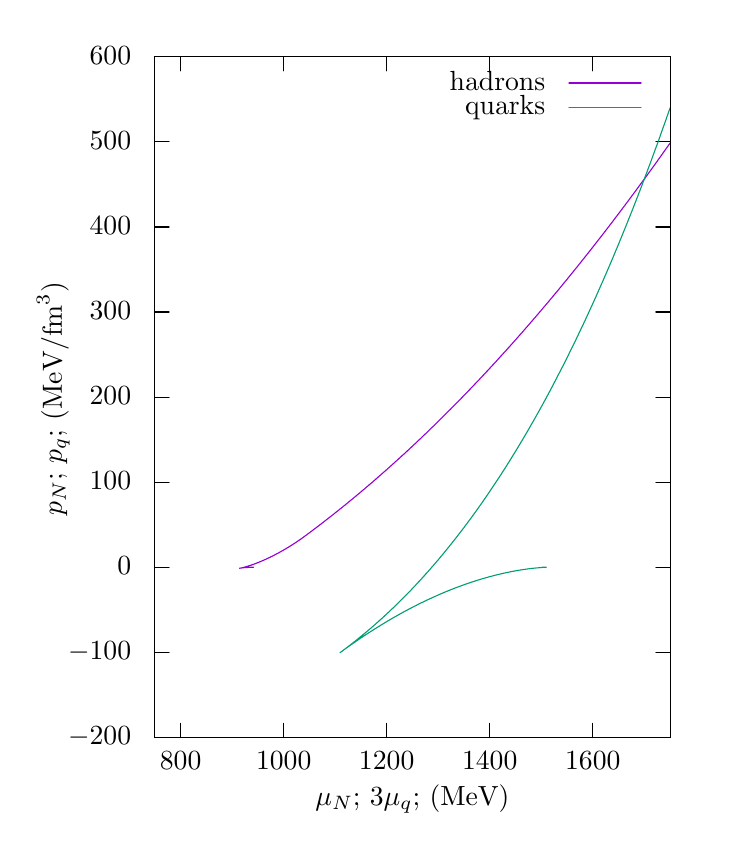
\begin{tikzpicture}[gnuplot]
%% generated with GNUPLOT 5.0p4 (Lua 5.2; terminal rev. 99, script rev. 100)
%% Thu Sep 29 16:33:18 2016
\path (0.000,0.000) rectangle (8.600,10.000);
\gpcolor{color=gp lt color border}
\gpsetlinetype{gp lt border}
\gpsetdashtype{gp dt solid}
\gpsetlinewidth{1.00}
\draw[gp path] (1.504,0.985)--(1.684,0.985);
\draw[gp path] (8.047,0.985)--(7.867,0.985);
\node[gp node right] at (1.320,0.985) {$-200$};
\draw[gp path] (1.504,2.066)--(1.684,2.066);
\draw[gp path] (8.047,2.066)--(7.867,2.066);
\node[gp node right] at (1.320,2.066) {$-100$};
\draw[gp path] (1.504,3.147)--(1.684,3.147);
\draw[gp path] (8.047,3.147)--(7.867,3.147);
\node[gp node right] at (1.320,3.147) {$0$};
\draw[gp path] (1.504,4.227)--(1.684,4.227);
\draw[gp path] (8.047,4.227)--(7.867,4.227);
\node[gp node right] at (1.320,4.227) {$100$};
\draw[gp path] (1.504,5.308)--(1.684,5.308);
\draw[gp path] (8.047,5.308)--(7.867,5.308);
\node[gp node right] at (1.320,5.308) {$200$};
\draw[gp path] (1.504,6.389)--(1.684,6.389);
\draw[gp path] (8.047,6.389)--(7.867,6.389);
\node[gp node right] at (1.320,6.389) {$300$};
\draw[gp path] (1.504,7.469)--(1.684,7.469);
\draw[gp path] (8.047,7.469)--(7.867,7.469);
\node[gp node right] at (1.320,7.469) {$400$};
\draw[gp path] (1.504,8.550)--(1.684,8.550);
\draw[gp path] (8.047,8.550)--(7.867,8.550);
\node[gp node right] at (1.320,8.550) {$500$};
\draw[gp path] (1.504,9.631)--(1.684,9.631);
\draw[gp path] (8.047,9.631)--(7.867,9.631);
\node[gp node right] at (1.320,9.631) {$600$};
\draw[gp path] (1.831,0.985)--(1.831,1.165);
\draw[gp path] (1.831,9.631)--(1.831,9.451);
\node[gp node center] at (1.831,0.677) {$800$};
\draw[gp path] (3.140,0.985)--(3.140,1.165);
\draw[gp path] (3.140,9.631)--(3.140,9.451);
\node[gp node center] at (3.140,0.677) {$1000$};
\draw[gp path] (4.448,0.985)--(4.448,1.165);
\draw[gp path] (4.448,9.631)--(4.448,9.451);
\node[gp node center] at (4.448,0.677) {$1200$};
\draw[gp path] (5.757,0.985)--(5.757,1.165);
\draw[gp path] (5.757,9.631)--(5.757,9.451);
\node[gp node center] at (5.757,0.677) {$1400$};
\draw[gp path] (7.066,0.985)--(7.066,1.165);
\draw[gp path] (7.066,9.631)--(7.066,9.451);
\node[gp node center] at (7.066,0.677) {$1600$};
\draw[gp path] (1.504,9.631)--(1.504,0.985)--(8.047,0.985)--(8.047,9.631)--cycle;
\node[gp node center,rotate=-270] at (0.246,5.308) {$p_N$; $p_q$; ($\rm{MeV}/\rm{fm}^3$)};
\node[gp node center] at (4.775,0.215) {$\mu_N$; $3\mu_q$; (MeV)};
\node[gp node right] at (6.579,9.297) {hadrons};
\gpcolor{rgb color={0.580,0.000,0.827}}
\draw[gp path] (6.763,9.297)--(7.679,9.297);
\draw[gp path] (2.725,3.146)--(2.732,3.146)--(2.739,3.146)--(2.745,3.147)--(2.751,3.147)%
  --(2.757,3.147)--(2.725,3.146)--(2.731,3.146)--(2.737,3.146)--(2.743,3.147)--(2.748,3.147)%
  --(2.716,3.146)--(2.721,3.146)--(2.727,3.146)--(2.732,3.146)--(2.738,3.147)--(2.705,3.146)%
  --(2.711,3.146)--(2.716,3.146)--(2.722,3.146)--(2.727,3.146)--(2.733,3.147)--(2.700,3.146)%
  --(2.706,3.146)--(2.711,3.146)--(2.717,3.146)--(2.722,3.146)--(2.690,3.145)--(2.695,3.145)%
  --(2.700,3.146)--(2.706,3.146)--(2.711,3.146)--(2.679,3.145)--(2.684,3.145)--(2.690,3.145)%
  --(2.695,3.145)--(2.700,3.146)--(2.706,3.146)--(2.673,3.145)--(2.679,3.145)--(2.684,3.145)%
  --(2.690,3.145)--(2.695,3.146)--(2.663,3.144)--(2.668,3.144)--(2.674,3.145)--(2.679,3.145)%
  --(2.685,3.145)--(2.690,3.145)--(2.658,3.144)--(2.663,3.144)--(2.669,3.144)--(2.674,3.145)%
  --(2.680,3.145)--(2.648,3.143)--(2.653,3.143)--(2.659,3.144)--(2.664,3.144)--(2.670,3.144)%
  --(2.675,3.145)--(2.643,3.143)--(2.649,3.143)--(2.654,3.143)--(2.660,3.144)--(2.665,3.144)%
  --(2.634,3.142)--(2.639,3.142)--(2.645,3.143)--(2.650,3.143)--(2.656,3.143)--(2.661,3.144)%
  --(2.630,3.141)--(2.635,3.142)--(2.641,3.142)--(2.647,3.143)--(2.652,3.143)--(2.621,3.141)%
  --(2.626,3.141)--(2.632,3.142)--(2.638,3.142)--(2.643,3.143)--(2.649,3.143)--(2.617,3.140)%
  --(2.623,3.141)--(2.629,3.141)--(2.635,3.142)--(2.640,3.142)--(2.609,3.139)--(2.615,3.140)%
  --(2.620,3.140)--(2.626,3.141)--(2.632,3.142)--(2.638,3.142)--(2.606,3.139)--(2.612,3.140)%
  --(2.618,3.140)--(2.624,3.141)--(2.630,3.141)--(2.635,3.142)--(2.604,3.139)--(2.610,3.139)%
  --(2.616,3.140)--(2.622,3.141)--(2.628,3.141)--(2.597,3.138)--(2.602,3.138)--(2.608,3.139)%
  --(2.614,3.140)--(2.620,3.140)--(2.626,3.141)--(2.595,3.137)--(2.601,3.138)--(2.607,3.139)%
  --(2.613,3.140)--(2.619,3.140)--(2.588,3.136)--(2.594,3.137)--(2.600,3.138)--(2.606,3.139)%
  --(2.612,3.140)--(2.618,3.140)--(2.587,3.136)--(2.593,3.137)--(2.599,3.138)--(2.605,3.139)%
  --(2.611,3.140)--(2.618,3.140)--(2.587,3.136)--(2.593,3.137)--(2.599,3.138)--(2.605,3.139)%
  --(2.611,3.140)--(2.617,3.140)--(2.587,3.136)--(2.593,3.137)--(2.599,3.138)--(2.605,3.139)%
  --(2.612,3.140)--(2.581,3.135)--(2.588,3.136)--(2.594,3.137)--(2.600,3.138)--(2.606,3.139)%
  --(2.612,3.140)--(2.582,3.135)--(2.588,3.136)--(2.595,3.137)--(2.601,3.138)--(2.607,3.139)%
  --(2.613,3.140)--(2.583,3.135)--(2.590,3.136)--(2.596,3.137)--(2.602,3.138)--(2.608,3.139)%
  --(2.579,3.134)--(2.585,3.135)--(2.591,3.136)--(2.597,3.138)--(2.604,3.139)--(2.610,3.140)%
  --(2.580,3.135)--(2.587,3.136)--(2.593,3.137)--(2.600,3.138)--(2.606,3.139)--(2.612,3.140)%
  --(2.583,3.135)--(2.589,3.136)--(2.596,3.137)--(2.602,3.138)--(2.608,3.140)--(2.615,3.141)%
  --(2.585,3.135)--(2.592,3.136)--(2.598,3.138)--(2.605,3.139)--(2.611,3.140)--(2.618,3.142)%
  --(2.588,3.136)--(2.595,3.137)--(2.601,3.138)--(2.608,3.140)--(2.614,3.141)--(2.585,3.135)%
  --(2.592,3.136)--(2.598,3.138)--(2.605,3.139)--(2.611,3.140)--(2.618,3.142)--(2.589,3.136)%
  --(2.596,3.137)--(2.602,3.138)--(2.609,3.140)--(2.615,3.141)--(2.622,3.143)--(2.593,3.136)%
  --(2.600,3.138)--(2.606,3.139)--(2.613,3.141)--(2.620,3.142)--(2.626,3.144)--(2.598,3.137)%
  --(2.604,3.139)--(2.611,3.140)--(2.618,3.142)--(2.624,3.143)--(2.596,3.137)--(2.603,3.138)%
  --(2.609,3.140)--(2.616,3.142)--(2.623,3.143)--(2.629,3.145)--(2.601,3.138)--(2.608,3.140)%
  --(2.614,3.141)--(2.621,3.143)--(2.628,3.144)--(2.635,3.146)--(2.607,3.139)--(2.613,3.141)%
  --(2.620,3.143)--(2.627,3.144)--(2.634,3.146)--(2.640,3.148)--(2.612,3.141)--(2.619,3.142)%
  --(2.626,3.144)--(2.633,3.146)--(2.640,3.147)--(2.647,3.149)--(2.619,3.142)--(2.626,3.144)%
  --(2.632,3.146)--(2.639,3.147)--(2.646,3.149)--(2.619,3.142)--(2.625,3.144)--(2.632,3.146)%
  --(2.639,3.147)--(2.646,3.149)--(2.653,3.151)--(2.625,3.144)--(2.632,3.146)--(2.639,3.147)%
  --(2.646,3.149)--(2.653,3.151)--(2.660,3.153)--(2.633,3.146)--(2.640,3.147)--(2.647,3.149)%
  --(2.654,3.151)--(2.661,3.153)--(2.668,3.155)--(2.640,3.148)--(2.648,3.150)--(2.655,3.152)%
  --(2.662,3.154)--(2.669,3.156)--(2.676,3.158)--(2.649,3.150)--(2.656,3.152)--(2.663,3.154)%
  --(2.670,3.156)--(2.677,3.158)--(2.650,3.150)--(2.657,3.152)--(2.664,3.154)--(2.671,3.156)%
  --(2.678,3.158)--(2.685,3.161)--(2.659,3.153)--(2.666,3.155)--(2.673,3.157)--(2.680,3.159)%
  --(2.687,3.161)--(2.694,3.163)--(2.668,3.155)--(2.675,3.157)--(2.682,3.160)--(2.689,3.162)%
  --(2.696,3.164)--(2.703,3.166)--(2.677,3.158)--(2.684,3.160)--(2.691,3.163)--(2.699,3.165)%
  --(2.706,3.167)--(2.679,3.159)--(2.687,3.161)--(2.694,3.163)--(2.701,3.166)--(2.708,3.168)%
  --(2.716,3.170)--(2.689,3.162)--(2.697,3.164)--(2.704,3.167)--(2.711,3.169)--(2.719,3.171)%
  --(2.726,3.174)--(2.700,3.165)--(2.707,3.168)--(2.714,3.170)--(2.722,3.173)--(2.729,3.175)%
  --(2.736,3.177)--(2.710,3.169)--(2.718,3.171)--(2.725,3.174)--(2.732,3.176)--(2.740,3.179)%
  --(2.714,3.170)--(2.722,3.172)--(2.729,3.175)--(2.736,3.178)--(2.744,3.180)--(2.751,3.183)%
  --(2.725,3.174)--(2.733,3.176)--(2.740,3.179)--(2.748,3.182)--(2.755,3.184)--(2.762,3.187)%
  --(2.737,3.178)--(2.745,3.180)--(2.752,3.183)--(2.759,3.186)--(2.767,3.188)--(2.742,3.179)%
  --(2.749,3.182)--(2.757,3.185)--(2.764,3.187)--(2.771,3.190)--(2.779,3.193)--(2.754,3.184)%
  --(2.761,3.187)--(2.769,3.189)--(2.776,3.192)--(2.784,3.195)--(2.767,3.189)--(2.775,3.191)%
  --(2.782,3.194)--(2.773,3.191)--(2.781,3.194)--(2.788,3.197)--(2.780,3.193)--(2.787,3.196)%
  --(2.795,3.199)--(2.786,3.196)--(2.794,3.199)--(2.801,3.202)--(2.793,3.198)--(2.801,3.201)%
  --(2.792,3.198)--(2.800,3.201)--(2.807,3.204)--(2.799,3.201)--(2.806,3.204)--(2.814,3.207)%
  --(2.806,3.203)--(2.813,3.206)--(2.821,3.209)--(2.813,3.206)--(2.820,3.209)--(2.812,3.206)%
  --(2.820,3.209)--(2.827,3.212)--(2.819,3.209)--(2.827,3.212)--(2.834,3.215)--(2.826,3.212)%
  --(2.834,3.215)--(2.841,3.218)--(2.833,3.215)--(2.841,3.218)--(2.833,3.214)--(2.841,3.218)%
  --(2.848,3.221)--(2.840,3.217)--(2.848,3.221)--(2.856,3.224)--(2.848,3.221)--(2.855,3.224)%
  --(2.848,3.220)--(2.855,3.224)--(2.863,3.227)--(2.855,3.224)--(2.863,3.227)--(2.871,3.230)%
  --(2.863,3.227)--(2.870,3.230)--(2.863,3.227)--(2.870,3.230)--(2.878,3.234)--(2.871,3.230)%
  --(2.878,3.234)--(2.886,3.237)--(2.878,3.234)--(2.886,3.237)--(2.879,3.234)--(2.886,3.237)%
  --(2.894,3.241)--(2.887,3.237)--(2.894,3.241)--(2.902,3.244)--(2.895,3.241)--(2.902,3.244)%
  --(2.895,3.241)--(2.903,3.244)--(2.910,3.248)--(2.903,3.245)--(2.911,3.248)--(2.919,3.252)%
  --(2.911,3.248)--(2.919,3.252)--(2.912,3.249)--(2.920,3.252)--(2.927,3.256)--(2.920,3.252)%
  --(2.928,3.256)--(2.921,3.253)--(2.929,3.256)--(2.937,3.260)--(2.929,3.257)--(2.937,3.260)%
  --(2.945,3.264)--(2.938,3.261)--(2.946,3.264)--(2.939,3.261)--(2.947,3.265)--(2.955,3.268)%
  --(2.948,3.265)--(2.955,3.269)--(2.949,3.266)--(2.956,3.269)--(2.964,3.273)--(2.957,3.270)%
  --(2.965,3.274)--(2.959,3.270)--(2.966,3.274)--(2.974,3.278)--(2.968,3.275)--(2.975,3.279)%
  --(2.969,3.275)--(2.977,3.279)--(2.984,3.283)--(2.978,3.280)--(2.986,3.284)--(2.979,3.280)%
  --(2.987,3.284)--(2.995,3.288)--(2.988,3.285)--(2.996,3.289)--(2.990,3.286)--(2.998,3.290)%
  --(3.006,3.294)--(2.999,3.290)--(3.007,3.294)--(3.001,3.291)--(3.009,3.295)--(3.017,3.299)%
  --(3.010,3.296)--(3.018,3.300)--(3.012,3.297)--(3.020,3.301)--(3.014,3.298)--(3.022,3.302)%
  --(3.030,3.306)--(3.024,3.303)--(3.031,3.307)--(3.025,3.304)--(3.033,3.308)--(3.041,3.312)%
  --(3.035,3.309)--(3.043,3.313)--(3.037,3.310)--(3.045,3.314)--(3.039,3.311)--(3.047,3.315)%
  --(3.055,3.319)--(3.049,3.316)--(3.057,3.320)--(3.052,3.317)--(3.060,3.322)--(3.054,3.319)%
  --(3.062,3.323)--(3.070,3.327)--(3.064,3.324)--(3.072,3.328)--(3.066,3.325)--(3.074,3.330)%
  --(3.069,3.327)--(3.077,3.331)--(3.085,3.335)--(3.079,3.332)--(3.087,3.337)--(3.082,3.334)%
  --(3.090,3.338)--(3.084,3.335)--(3.092,3.339)--(3.100,3.344)--(3.095,3.341)--(3.103,3.345)%
  --(3.098,3.342)--(3.106,3.347)--(3.101,3.344)--(3.109,3.348)--(3.103,3.346)--(3.111,3.350)%
  --(3.106,3.347)--(3.114,3.352)--(3.122,3.356)--(3.117,3.353)--(3.125,3.358)--(3.120,3.355)%
  --(3.128,3.360)--(3.124,3.357)--(3.132,3.361)--(3.127,3.359)--(3.135,3.363)--(3.130,3.361)%
  --(3.138,3.365)--(3.133,3.362)--(3.141,3.367)--(3.149,3.372)--(3.145,3.369)--(3.153,3.374)%
  --(3.148,3.371)--(3.156,3.376)--(3.152,3.373)--(3.160,3.378)--(3.155,3.375)--(3.163,3.380)%
  --(3.159,3.377)--(3.167,3.382)--(3.163,3.379)--(3.171,3.384)--(3.166,3.382)--(3.174,3.386)%
  --(3.170,3.384)--(3.178,3.389)--(3.174,3.386)--(3.182,3.391)--(3.178,3.389)--(3.186,3.393)%
  --(3.182,3.391)--(3.190,3.396)--(3.186,3.394)--(3.194,3.398)--(3.190,3.396)--(3.198,3.401)%
  --(3.195,3.399)--(3.203,3.404)--(3.199,3.401)--(3.207,3.406)--(3.203,3.404)--(3.211,3.409)%
  --(3.208,3.407)--(3.216,3.412)--(3.212,3.410)--(3.220,3.414)--(3.217,3.412)--(3.225,3.417)%
  --(3.222,3.415)--(3.218,3.413)--(3.226,3.418)--(3.223,3.416)--(3.231,3.421)--(3.228,3.419)%
  --(3.236,3.424)--(3.233,3.422)--(3.241,3.427)--(3.238,3.426)--(3.246,3.431)--(3.243,3.429)%
  --(3.246,3.430)--(3.248,3.432)--(3.251,3.434)--(3.254,3.436)--(3.256,3.437)--(3.254,3.436)%
  --(3.257,3.437)--(3.259,3.439)--(3.262,3.441)--(3.265,3.443)--(3.268,3.445)--(3.266,3.443)%
  --(3.269,3.445)--(3.271,3.447)--(3.274,3.449)--(3.272,3.447)--(3.275,3.449)--(3.278,3.451)%
  --(3.281,3.453)--(3.284,3.455)--(3.283,3.454)--(3.286,3.456)--(3.289,3.458)--(3.287,3.457)%
  --(3.290,3.459)--(3.294,3.461)--(3.297,3.464)--(3.295,3.463)--(3.299,3.465)--(3.302,3.467)%
  --(3.301,3.466)--(3.304,3.468)--(3.308,3.471)--(3.306,3.470)--(3.310,3.472)--(3.309,3.472)%
  --(3.313,3.474)--(3.316,3.477)--(3.315,3.476)--(3.319,3.478)--(3.318,3.478)--(3.322,3.481)%
  --(3.321,3.480)--(3.325,3.483)--(3.329,3.485)--(3.332,3.488)--(3.336,3.490)--(3.337,3.491)%
  --(3.341,3.493)--(3.341,3.494)--(3.346,3.497)--(3.347,3.498)--(3.348,3.498)--(3.352,3.501)%
  --(3.353,3.502)--(3.354,3.503)--(3.355,3.504)--(3.356,3.504)--(3.358,3.505)--(3.359,3.506)%
  --(3.361,3.507)--(3.362,3.509)--(3.365,3.510)--(3.367,3.512)--(3.369,3.514)--(3.370,3.514)%
  --(3.373,3.516)--(3.374,3.517)--(3.375,3.518)--(3.377,3.519)--(3.378,3.520)--(3.380,3.521)%
  --(3.381,3.522)--(3.383,3.524)--(3.385,3.525)--(3.387,3.526)--(3.388,3.527)--(3.390,3.529)%
  --(3.391,3.529)--(3.393,3.531)--(3.394,3.532)--(3.396,3.533)--(3.397,3.534)--(3.398,3.535)%
  --(3.400,3.536)--(3.406,3.540)--(3.414,3.546)--(3.421,3.552)--(3.429,3.557)--(3.437,3.563)%
  --(3.445,3.569)--(3.452,3.575)--(3.460,3.580)--(3.468,3.586)--(3.476,3.592)--(3.483,3.598)%
  --(3.491,3.604)--(3.499,3.609)--(3.507,3.615)--(3.514,3.621)--(3.522,3.627)--(3.530,3.633)%
  --(3.537,3.639)--(3.545,3.644)--(3.553,3.650)--(3.561,3.656)--(3.568,3.662)--(3.576,3.668)%
  --(3.584,3.674)--(3.592,3.680)--(3.599,3.686)--(3.607,3.691)--(3.615,3.697)--(3.622,3.703)%
  --(3.630,3.709)--(3.638,3.715)--(3.646,3.721)--(3.653,3.727)--(3.661,3.733)--(3.669,3.739)%
  --(3.676,3.745)--(3.684,3.751)--(3.692,3.757)--(3.699,3.763)--(3.707,3.769)--(3.715,3.775)%
  --(3.723,3.781)--(3.730,3.787)--(3.738,3.793)--(3.746,3.799)--(3.753,3.805)--(3.761,3.811)%
  --(3.769,3.817)--(3.776,3.823)--(3.784,3.830)--(3.792,3.836)--(3.800,3.842)--(3.807,3.848)%
  --(3.815,3.854)--(3.823,3.860)--(3.830,3.866)--(3.838,3.872)--(3.846,3.879)--(3.853,3.885)%
  --(3.861,3.891)--(3.869,3.897)--(3.876,3.903)--(3.884,3.909)--(3.892,3.916)--(3.899,3.922)%
  --(3.907,3.928)--(3.915,3.934)--(3.922,3.940)--(3.930,3.947)--(3.938,3.953)--(3.945,3.959)%
  --(3.953,3.965)--(3.961,3.972)--(3.968,3.978)--(3.976,3.984)--(3.984,3.991)--(3.991,3.997)%
  --(3.999,4.003)--(4.007,4.009)--(4.014,4.016)--(4.022,4.022)--(4.030,4.028)--(4.037,4.035)%
  --(4.045,4.041)--(4.053,4.047)--(4.060,4.054)--(4.068,4.060)--(4.076,4.067)--(4.083,4.073)%
  --(4.091,4.079)--(4.099,4.086)--(4.106,4.092)--(4.114,4.099)--(4.122,4.105)--(4.129,4.111)%
  --(4.137,4.118)--(4.144,4.124)--(4.152,4.131)--(4.160,4.137)--(4.167,4.144)--(4.175,4.150)%
  --(4.183,4.157)--(4.190,4.163)--(4.198,4.170)--(4.206,4.176)--(4.213,4.183)--(4.221,4.189)%
  --(4.228,4.196)--(4.236,4.202)--(4.244,4.209)--(4.251,4.215)--(4.259,4.222)--(4.267,4.228)%
  --(4.274,4.235)--(4.282,4.242)--(4.289,4.248)--(4.297,4.255)--(4.305,4.261)--(4.312,4.268)%
  --(4.320,4.275)--(4.328,4.281)--(4.335,4.288)--(4.343,4.295)--(4.350,4.301)--(4.358,4.308)%
  --(4.366,4.315)--(4.373,4.321)--(4.381,4.328)--(4.389,4.335)--(4.396,4.341)--(4.404,4.348)%
  --(4.411,4.355)--(4.419,4.361)--(4.427,4.368)--(4.434,4.375)--(4.442,4.382)--(4.449,4.388)%
  --(4.457,4.395)--(4.465,4.402)--(4.472,4.409)--(4.480,4.415)--(4.487,4.422)--(4.495,4.429)%
  --(4.503,4.436)--(4.510,4.443)--(4.518,4.449)--(4.525,4.456)--(4.533,4.463)--(4.541,4.470)%
  --(4.548,4.477)--(4.556,4.484)--(4.563,4.491)--(4.571,4.497)--(4.579,4.504)--(4.586,4.511)%
  --(4.594,4.518)--(4.601,4.525)--(4.609,4.532)--(4.617,4.539)--(4.624,4.546)--(4.632,4.553)%
  --(4.639,4.560)--(4.647,4.567)--(4.654,4.574)--(4.662,4.580)--(4.670,4.587)--(4.677,4.594)%
  --(4.685,4.601)--(4.692,4.608)--(4.700,4.615)--(4.708,4.622)--(4.715,4.629)--(4.723,4.636)%
  --(4.730,4.643)--(4.738,4.651)--(4.745,4.658)--(4.753,4.665)--(4.761,4.672)--(4.768,4.679)%
  --(4.776,4.686)--(4.783,4.693)--(4.791,4.700)--(4.798,4.707)--(4.806,4.714)--(4.814,4.721)%
  --(4.821,4.728)--(4.829,4.736)--(4.836,4.743)--(4.844,4.750)--(4.851,4.757)--(4.859,4.764)%
  --(4.866,4.771)--(4.874,4.778)--(4.882,4.786)--(4.889,4.793)--(4.897,4.800)--(4.904,4.807)%
  --(4.912,4.814)--(4.919,4.822)--(4.927,4.829)--(4.934,4.836)--(4.942,4.843)--(4.950,4.851)%
  --(4.957,4.858)--(4.965,4.865)--(4.972,4.872)--(4.980,4.880)--(4.987,4.887)--(4.995,4.894)%
  --(5.002,4.902)--(5.010,4.909)--(5.017,4.916)--(5.025,4.924)--(5.033,4.931)--(5.040,4.938)%
  --(5.048,4.946)--(5.055,4.953)--(5.063,4.960)--(5.070,4.968)--(5.078,4.975)--(5.085,4.982)%
  --(5.093,4.990)--(5.100,4.997)--(5.108,5.005)--(5.116,5.012)--(5.123,5.019)--(5.131,5.027)%
  --(5.138,5.034)--(5.146,5.042)--(5.153,5.049)--(5.161,5.057)--(5.168,5.064)--(5.176,5.072)%
  --(5.183,5.079)--(5.191,5.087)--(5.198,5.094)--(5.206,5.102)--(5.213,5.109)--(5.221,5.117)%
  --(5.228,5.124)--(5.236,5.132)--(5.243,5.139)--(5.251,5.147)--(5.259,5.154)--(5.266,5.162)%
  --(5.274,5.170)--(5.281,5.177)--(5.289,5.185)--(5.296,5.192)--(5.304,5.200)--(5.311,5.208)%
  --(5.319,5.215)--(5.326,5.223)--(5.334,5.230)--(5.341,5.238)--(5.349,5.246)--(5.356,5.253)%
  --(5.364,5.261)--(5.371,5.269)--(5.379,5.276)--(5.386,5.284)--(5.394,5.292)--(5.401,5.300)%
  --(5.409,5.307)--(5.416,5.315)--(5.424,5.323)--(5.431,5.330)--(5.439,5.338)--(5.446,5.346)%
  --(5.454,5.354)--(5.461,5.361)--(5.469,5.369)--(5.476,5.377)--(5.484,5.385)--(5.491,5.393)%
  --(5.499,5.400)--(5.506,5.408)--(5.514,5.416)--(5.521,5.424)--(5.529,5.432)--(5.536,5.439)%
  --(5.544,5.447)--(5.551,5.455)--(5.559,5.463)--(5.566,5.471)--(5.574,5.479)--(5.581,5.487)%
  --(5.589,5.495)--(5.596,5.502)--(5.604,5.510)--(5.611,5.518)--(5.619,5.526)--(5.626,5.534)%
  --(5.634,5.542)--(5.641,5.550)--(5.649,5.558)--(5.656,5.566)--(5.664,5.574)--(5.671,5.582)%
  --(5.679,5.590)--(5.686,5.598)--(5.694,5.606)--(5.701,5.614)--(5.709,5.622)--(5.716,5.630)%
  --(5.724,5.638)--(5.731,5.646)--(5.738,5.654)--(5.746,5.662)--(5.753,5.670)--(5.761,5.678)%
  --(5.768,5.686)--(5.776,5.694)--(5.783,5.702)--(5.791,5.711)--(5.798,5.719)--(5.806,5.727)%
  --(5.813,5.735)--(5.821,5.743)--(5.828,5.751)--(5.836,5.759)--(5.843,5.767)--(5.851,5.776)%
  --(5.858,5.784)--(5.865,5.792)--(5.873,5.800)--(5.880,5.808)--(5.888,5.816)--(5.895,5.825)%
  --(5.903,5.833)--(5.910,5.841)--(5.918,5.849)--(5.925,5.858)--(5.933,5.866)--(5.940,5.874)%
  --(5.948,5.882)--(5.955,5.891)--(5.963,5.899)--(5.970,5.907)--(5.977,5.915)--(5.985,5.924)%
  --(5.992,5.932)--(6.000,5.940)--(6.007,5.949)--(6.015,5.957)--(6.022,5.965)--(6.030,5.974)%
  --(6.037,5.982)--(6.045,5.990)--(6.052,5.999)--(6.059,6.007)--(6.067,6.015)--(6.074,6.024)%
  --(6.082,6.032)--(6.089,6.041)--(6.097,6.049)--(6.104,6.057)--(6.112,6.066)--(6.119,6.074)%
  --(6.126,6.083)--(6.134,6.091)--(6.141,6.100)--(6.149,6.108)--(6.156,6.117)--(6.164,6.125)%
  --(6.171,6.133)--(6.179,6.142)--(6.186,6.150)--(6.193,6.159)--(6.201,6.167)--(6.208,6.176)%
  --(6.216,6.185)--(6.223,6.193)--(6.231,6.202)--(6.238,6.210)--(6.246,6.219)--(6.253,6.227)%
  --(6.260,6.236)--(6.268,6.244)--(6.275,6.253)--(6.283,6.262)--(6.290,6.270)--(6.298,6.279)%
  --(6.305,6.287)--(6.312,6.296)--(6.320,6.305)--(6.327,6.313)--(6.335,6.322)--(6.342,6.331)%
  --(6.350,6.339)--(6.357,6.348)--(6.364,6.357)--(6.372,6.365)--(6.379,6.374)--(6.387,6.383)%
  --(6.394,6.391)--(6.402,6.400)--(6.409,6.409)--(6.416,6.418)--(6.424,6.426)--(6.431,6.435)%
  --(6.439,6.444)--(6.446,6.453)--(6.454,6.461)--(6.461,6.470)--(6.468,6.479)--(6.476,6.488)%
  --(6.483,6.496)--(6.491,6.505)--(6.498,6.514)--(6.505,6.523)--(6.513,6.532)--(6.520,6.541)%
  --(6.528,6.549)--(6.535,6.558)--(6.543,6.567)--(6.550,6.576)--(6.557,6.585)--(6.565,6.594)%
  --(6.572,6.603)--(6.580,6.612)--(6.587,6.620)--(6.594,6.629)--(6.602,6.638)--(6.609,6.647)%
  --(6.617,6.656)--(6.624,6.665)--(6.631,6.674)--(6.639,6.683)--(6.646,6.692)--(6.654,6.701)%
  --(6.661,6.710)--(6.669,6.719)--(6.676,6.728)--(6.683,6.737)--(6.691,6.746)--(6.698,6.755)%
  --(6.706,6.764)--(6.713,6.773)--(6.720,6.782)--(6.728,6.791)--(6.735,6.800)--(6.743,6.809)%
  --(6.750,6.818)--(6.757,6.827)--(6.765,6.836)--(6.772,6.845)--(6.780,6.855)--(6.787,6.864)%
  --(6.794,6.873)--(6.802,6.882)--(6.809,6.891)--(6.817,6.900)--(6.824,6.909)--(6.831,6.918)%
  --(6.839,6.928)--(6.846,6.937)--(6.853,6.946)--(6.861,6.955)--(6.868,6.964)--(6.876,6.973)%
  --(6.883,6.983)--(6.890,6.992)--(6.898,7.001)--(6.905,7.010)--(6.913,7.020)--(6.920,7.029)%
  --(6.927,7.038)--(6.935,7.047)--(6.942,7.057)--(6.950,7.066)--(6.957,7.075)--(6.964,7.084)%
  --(6.972,7.094)--(6.979,7.103)--(6.986,7.112)--(6.994,7.122)--(7.001,7.131)--(7.009,7.140)%
  --(7.016,7.150)--(7.023,7.159)--(7.031,7.168)--(7.038,7.178)--(7.046,7.187)--(7.053,7.196)%
  --(7.060,7.206)--(7.068,7.215)--(7.075,7.225)--(7.082,7.234)--(7.090,7.243)--(7.097,7.253)%
  --(7.105,7.262)--(7.112,7.272)--(7.119,7.281)--(7.127,7.291)--(7.134,7.300)--(7.141,7.310)%
  --(7.149,7.319)--(7.156,7.328)--(7.164,7.338)--(7.171,7.347)--(7.178,7.357)--(7.186,7.366)%
  --(7.193,7.376)--(7.200,7.386)--(7.208,7.395)--(7.215,7.405)--(7.223,7.414)--(7.230,7.424)%
  --(7.237,7.433)--(7.245,7.443)--(7.252,7.452)--(7.259,7.462)--(7.267,7.472)--(7.274,7.481)%
  --(7.281,7.491)--(7.289,7.500)--(7.296,7.510)--(7.304,7.520)--(7.311,7.529)--(7.318,7.539)%
  --(7.326,7.549)--(7.333,7.558)--(7.340,7.568)--(7.348,7.578)--(7.355,7.587)--(7.362,7.597)%
  --(7.370,7.607)--(7.377,7.616)--(7.384,7.626)--(7.392,7.636)--(7.399,7.646)--(7.407,7.655)%
  --(7.414,7.665)--(7.421,7.675)--(7.429,7.685)--(7.436,7.694)--(7.443,7.704)--(7.451,7.714)%
  --(7.458,7.724)--(7.465,7.733)--(7.473,7.743)--(7.480,7.753)--(7.487,7.763)--(7.495,7.773)%
  --(7.502,7.783)--(7.510,7.792)--(7.517,7.802)--(7.524,7.812)--(7.532,7.822)--(7.539,7.832)%
  --(7.546,7.842)--(7.554,7.852)--(7.561,7.862)--(7.568,7.871)--(7.576,7.881)--(7.583,7.891)%
  --(7.590,7.901)--(7.598,7.911)--(7.605,7.921)--(7.612,7.931)--(7.620,7.941)--(7.627,7.951)%
  --(7.634,7.961)--(7.642,7.971)--(7.649,7.981)--(7.656,7.991)--(7.664,8.001)--(7.671,8.011)%
  --(7.678,8.021)--(7.686,8.031)--(7.693,8.041)--(7.700,8.051)--(7.708,8.061)--(7.715,8.071)%
  --(7.723,8.081)--(7.730,8.091)--(7.737,8.101)--(7.745,8.111)--(7.752,8.121)--(7.759,8.131)%
  --(7.767,8.142)--(7.774,8.152)--(7.781,8.162)--(7.789,8.172)--(7.796,8.182)--(7.803,8.192)%
  --(7.811,8.202)--(7.818,8.213)--(7.825,8.223)--(7.833,8.233)--(7.840,8.243)--(7.847,8.253)%
  --(7.855,8.263)--(7.862,8.274)--(7.869,8.284)--(7.877,8.294)--(7.884,8.304)--(7.891,8.314)%
  --(7.898,8.325)--(7.906,8.335)--(7.913,8.345)--(7.920,8.355)--(7.928,8.366)--(7.935,8.376)%
  --(7.942,8.386)--(7.950,8.397)--(7.957,8.407)--(7.964,8.417)--(7.972,8.428)--(7.979,8.438)%
  --(7.986,8.448)--(7.994,8.459)--(8.001,8.469)--(8.008,8.479)--(8.016,8.490)--(8.023,8.500)%
  --(8.030,8.510)--(8.038,8.521)--(8.045,8.531)--(8.047,8.534);
\gpcolor{color=gp lt color border}
\node[gp node right] at (6.579,8.989) {quarks};
\gpcolor{rgb color={0.000,0.620,0.451}}
\draw[gp path] (6.763,8.989)--(7.679,8.989);
\draw[gp path] (6.423,3.147)--(6.445,3.147)--(6.457,3.147)--(6.465,3.147)--(6.470,3.147)%
  --(6.473,3.147)--(6.475,3.147)--(6.476,3.147)--(6.475,3.147)--(6.474,3.147)--(6.472,3.147)%
  --(6.470,3.147)--(6.467,3.147)--(6.463,3.146)--(6.460,3.146)--(6.455,3.146)--(6.451,3.146)%
  --(6.446,3.146)--(6.440,3.145)--(6.435,3.145)--(6.429,3.145)--(6.423,3.144)--(6.417,3.144)%
  --(6.410,3.144)--(6.404,3.143)--(6.397,3.143)--(6.390,3.142)--(6.383,3.141)--(6.376,3.141)%
  --(6.368,3.140)--(6.361,3.140)--(6.353,3.139)--(6.345,3.138)--(6.337,3.137)--(6.329,3.137)%
  --(6.321,3.136)--(6.313,3.135)--(6.304,3.134)--(6.296,3.133)--(6.287,3.132)--(6.279,3.131)%
  --(6.270,3.130)--(6.261,3.129)--(6.252,3.128)--(6.243,3.126)--(6.234,3.125)--(6.225,3.124)%
  --(6.216,3.123)--(6.207,3.121)--(6.197,3.120)--(6.188,3.119)--(6.179,3.117)--(6.169,3.116)%
  --(6.159,3.114)--(6.150,3.113)--(6.140,3.111)--(6.130,3.110)--(6.121,3.108)--(6.111,3.106)%
  --(6.101,3.105)--(6.091,3.103)--(6.081,3.101)--(6.071,3.099)--(6.061,3.097)--(6.051,3.096)%
  --(6.041,3.094)--(6.030,3.092)--(6.020,3.090)--(6.010,3.087)--(6.000,3.085)--(5.989,3.083)%
  --(5.979,3.081)--(5.968,3.079)--(5.958,3.077)--(5.947,3.074)--(5.937,3.072)--(5.926,3.070)%
  --(5.916,3.067)--(5.905,3.065)--(5.894,3.062)--(5.884,3.060)--(5.873,3.057)--(5.862,3.055)%
  --(5.851,3.052)--(5.841,3.049)--(5.830,3.047)--(5.819,3.044)--(5.808,3.041)--(5.797,3.038)%
  --(5.786,3.035)--(5.775,3.032)--(5.764,3.030)--(5.753,3.027)--(5.742,3.024)--(5.731,3.020)%
  --(5.720,3.017)--(5.709,3.014)--(5.698,3.011)--(5.687,3.008)--(5.675,3.005)--(5.664,3.001)%
  --(5.653,2.998)--(5.642,2.995)--(5.630,2.991)--(5.619,2.988)--(5.608,2.984)--(5.596,2.981)%
  --(5.585,2.977)--(5.574,2.973)--(5.562,2.970)--(5.551,2.966)--(5.539,2.962)--(5.528,2.959)%
  --(5.517,2.955)--(5.505,2.951)--(5.494,2.947)--(5.482,2.943)--(5.471,2.939)--(5.459,2.935)%
  --(5.447,2.931)--(5.436,2.927)--(5.424,2.923)--(5.413,2.919)--(5.401,2.914)--(5.389,2.910)%
  --(5.378,2.906)--(5.366,2.902)--(5.354,2.897)--(5.343,2.893)--(5.331,2.888)--(5.319,2.884)%
  --(5.307,2.879)--(5.296,2.875)--(5.284,2.870)--(5.272,2.866)--(5.260,2.861)--(5.249,2.856)%
  --(5.237,2.851)--(5.225,2.847)--(5.213,2.842)--(5.201,2.837)--(5.189,2.832)--(5.177,2.827)%
  --(5.166,2.822)--(5.154,2.817)--(5.142,2.812)--(5.130,2.807)--(5.118,2.801)--(5.106,2.796)%
  --(5.094,2.791)--(5.082,2.786)--(5.070,2.780)--(5.058,2.775)--(5.046,2.770)--(5.034,2.764)%
  --(5.022,2.759)--(5.010,2.753)--(4.998,2.748)--(4.986,2.742)--(4.973,2.736)--(4.961,2.731)%
  --(4.949,2.725)--(4.937,2.719)--(4.925,2.713)--(4.913,2.707)--(4.901,2.702)--(4.889,2.696)%
  --(4.877,2.690)--(4.864,2.684)--(4.852,2.678)--(4.840,2.672)--(4.828,2.665)--(4.816,2.659)%
  --(4.803,2.653)--(4.791,2.647)--(4.779,2.640)--(4.767,2.634)--(4.754,2.628)--(4.742,2.621)%
  --(4.730,2.615)--(4.718,2.608)--(4.705,2.602)--(4.693,2.595)--(4.681,2.589)--(4.669,2.582)%
  --(4.656,2.575)--(4.644,2.569)--(4.632,2.562)--(4.619,2.555)--(4.607,2.548)--(4.595,2.541)%
  --(4.582,2.534)--(4.570,2.527)--(4.558,2.520)--(4.545,2.513)--(4.533,2.506)--(4.520,2.499)%
  --(4.508,2.492)--(4.496,2.484)--(4.483,2.477)--(4.471,2.470)--(4.458,2.463)--(4.446,2.455)%
  --(4.433,2.448)--(4.421,2.440)--(4.409,2.433)--(4.396,2.425)--(4.384,2.418)--(4.371,2.410)%
  --(4.359,2.402)--(4.346,2.395)--(4.334,2.387)--(4.321,2.379)--(4.309,2.371)--(4.296,2.363)%
  --(4.284,2.355)--(4.271,2.347)--(4.259,2.339)--(4.246,2.331)--(4.233,2.323)--(4.221,2.315)%
  --(4.208,2.307)--(4.196,2.299)--(4.183,2.291)--(4.171,2.282)--(4.158,2.274)--(4.146,2.266)%
  --(4.133,2.257)--(4.120,2.249)--(4.108,2.240)--(4.095,2.232)--(4.083,2.223)--(4.070,2.215)%
  --(4.057,2.206)--(4.045,2.197)--(4.032,2.188)--(4.019,2.180)--(4.007,2.171)--(3.994,2.162)%
  --(3.981,2.153)--(3.969,2.144)--(3.956,2.135)--(3.943,2.126)--(3.931,2.117)--(3.918,2.108)%
  --(3.905,2.099)--(3.893,2.090)--(3.880,2.080)--(3.867,2.071)--(3.855,2.062)--(3.864,2.069)%
  --(3.874,2.076)--(3.884,2.083)--(3.893,2.090)--(3.903,2.098)--(3.912,2.105)--(3.922,2.112)%
  --(3.931,2.119)--(3.941,2.126)--(3.950,2.133)--(3.960,2.141)--(3.969,2.148)--(3.979,2.155)%
  --(3.988,2.162)--(3.997,2.170)--(4.007,2.177)--(4.016,2.184)--(4.025,2.191)--(4.034,2.199)%
  --(4.044,2.206)--(4.053,2.213)--(4.062,2.221)--(4.071,2.228)--(4.080,2.235)--(4.089,2.243)%
  --(4.098,2.250)--(4.107,2.257)--(4.116,2.265)--(4.126,2.272)--(4.135,2.280)--(4.143,2.287)%
  --(4.152,2.294)--(4.161,2.302)--(4.170,2.309)--(4.179,2.317)--(4.188,2.324)--(4.197,2.331)%
  --(4.206,2.339)--(4.215,2.346)--(4.223,2.354)--(4.232,2.361)--(4.241,2.369)--(4.250,2.376)%
  --(4.258,2.384)--(4.267,2.391)--(4.276,2.399)--(4.284,2.406)--(4.293,2.414)--(4.302,2.421)%
  --(4.310,2.429)--(4.319,2.437)--(4.327,2.444)--(4.336,2.452)--(4.344,2.459)--(4.353,2.467)%
  --(4.361,2.475)--(4.370,2.482)--(4.378,2.490)--(4.387,2.497)--(4.395,2.505)--(4.403,2.513)%
  --(4.412,2.520)--(4.420,2.528)--(4.428,2.536)--(4.437,2.543)--(4.445,2.551)--(4.453,2.559)%
  --(4.462,2.567)--(4.470,2.574)--(4.478,2.582)--(4.486,2.590)--(4.495,2.597)--(4.503,2.605)%
  --(4.511,2.613)--(4.519,2.621)--(4.527,2.628)--(4.535,2.636)--(4.543,2.644)--(4.551,2.652)%
  --(4.559,2.660)--(4.568,2.667)--(4.576,2.675)--(4.584,2.683)--(4.592,2.691)--(4.600,2.699)%
  --(4.608,2.707)--(4.615,2.714)--(4.623,2.722)--(4.631,2.730)--(4.639,2.738)--(4.647,2.746)%
  --(4.655,2.754)--(4.663,2.762)--(4.671,2.770)--(4.678,2.778)--(4.686,2.786)--(4.694,2.793)%
  --(4.702,2.801)--(4.710,2.809)--(4.717,2.817)--(4.725,2.825)--(4.733,2.833)--(4.741,2.841)%
  --(4.748,2.849)--(4.756,2.857)--(4.764,2.865)--(4.771,2.873)--(4.779,2.881)--(4.787,2.889)%
  --(4.794,2.897)--(4.802,2.905)--(4.809,2.913)--(4.817,2.921)--(4.824,2.930)--(4.832,2.938)%
  --(4.839,2.946)--(4.847,2.954)--(4.854,2.962)--(4.862,2.970)--(4.869,2.978)--(4.877,2.986)%
  --(4.884,2.994)--(4.892,3.002)--(4.899,3.011)--(4.907,3.019)--(4.914,3.027)--(4.921,3.035)%
  --(4.929,3.043)--(4.936,3.051)--(4.943,3.060)--(4.951,3.068)--(4.958,3.076)--(4.965,3.084)%
  --(4.973,3.092)--(4.980,3.101)--(4.987,3.109)--(4.994,3.117)--(5.002,3.125)--(5.009,3.134)%
  --(5.016,3.142)--(5.023,3.150)--(5.030,3.158)--(5.038,3.167)--(5.045,3.175)--(5.052,3.183)%
  --(5.059,3.191)--(5.066,3.200)--(5.073,3.208)--(5.080,3.216)--(5.087,3.225)--(5.095,3.233)%
  --(5.102,3.241)--(5.109,3.250)--(5.116,3.258)--(5.123,3.266)--(5.130,3.275)--(5.137,3.283)%
  --(5.144,3.291)--(5.151,3.300)--(5.158,3.308)--(5.165,3.317)--(5.172,3.325)--(5.179,3.333)%
  --(5.185,3.342)--(5.192,3.350)--(5.199,3.359)--(5.206,3.367)--(5.213,3.376)--(5.220,3.384)%
  --(5.227,3.393)--(5.234,3.401)--(5.241,3.409)--(5.247,3.418)--(5.254,3.426)--(5.261,3.435)%
  --(5.268,3.443)--(5.275,3.452)--(5.281,3.460)--(5.288,3.469)--(5.295,3.477)--(5.302,3.486)%
  --(5.308,3.495)--(5.315,3.503)--(5.322,3.512)--(5.328,3.520)--(5.335,3.529)--(5.342,3.537)%
  --(5.349,3.546)--(5.355,3.555)--(5.362,3.563)--(5.368,3.572)--(5.375,3.580)--(5.382,3.589)%
  --(5.388,3.598)--(5.395,3.606)--(5.402,3.615)--(5.408,3.623)--(5.415,3.632)--(5.421,3.641)%
  --(5.428,3.649)--(5.434,3.658)--(5.441,3.667)--(5.447,3.675)--(5.454,3.684)--(5.460,3.693)%
  --(5.467,3.701)--(5.473,3.710)--(5.480,3.719)--(5.486,3.728)--(5.493,3.736)--(5.499,3.745)%
  --(5.506,3.754)--(5.512,3.762)--(5.519,3.771)--(5.525,3.780)--(5.531,3.789)--(5.538,3.797)%
  --(5.544,3.806)--(5.551,3.815)--(5.557,3.824)--(5.563,3.833)--(5.570,3.841)--(5.576,3.850)%
  --(5.582,3.859)--(5.589,3.868)--(5.595,3.877)--(5.601,3.885)--(5.607,3.894)--(5.614,3.903)%
  --(5.620,3.912)--(5.626,3.921)--(5.633,3.930)--(5.639,3.939)--(5.645,3.947)--(5.651,3.956)%
  --(5.658,3.965)--(5.664,3.974)--(5.670,3.983)--(5.676,3.992)--(5.682,4.001)--(5.688,4.010)%
  --(5.695,4.019)--(5.701,4.027)--(5.707,4.036)--(5.713,4.045)--(5.719,4.054)--(5.725,4.063)%
  --(5.732,4.072)--(5.738,4.081)--(5.744,4.090)--(5.750,4.099)--(5.756,4.108)--(5.762,4.117)%
  --(5.768,4.126)--(5.774,4.135)--(5.780,4.144)--(5.786,4.153)--(5.792,4.162)--(5.798,4.171)%
  --(5.804,4.180)--(5.810,4.189)--(5.816,4.198)--(5.822,4.207)--(5.828,4.216)--(5.834,4.225)%
  --(5.840,4.234)--(5.846,4.243)--(5.852,4.253)--(5.858,4.262)--(5.864,4.271)--(5.870,4.280)%
  --(5.876,4.289)--(5.882,4.298)--(5.888,4.307)--(5.894,4.316)--(5.900,4.325)--(5.906,4.334)%
  --(5.912,4.344)--(5.917,4.353)--(5.923,4.362)--(5.929,4.371)--(5.935,4.380)--(5.941,4.389)%
  --(5.947,4.398)--(5.953,4.408)--(5.958,4.417)--(5.964,4.426)--(5.970,4.435)--(5.976,4.444)%
  --(5.982,4.454)--(5.987,4.463)--(5.993,4.472)--(5.999,4.481)--(6.005,4.490)--(6.011,4.500)%
  --(6.016,4.509)--(6.022,4.518)--(6.028,4.527)--(6.034,4.537)--(6.039,4.546)--(6.045,4.555)%
  --(6.051,4.564)--(6.056,4.574)--(6.062,4.583)--(6.068,4.592)--(6.074,4.602)--(6.079,4.611)%
  --(6.085,4.620)--(6.091,4.629)--(6.096,4.639)--(6.102,4.648)--(6.108,4.657)--(6.113,4.667)%
  --(6.119,4.676)--(6.124,4.685)--(6.130,4.695)--(6.136,4.704)--(6.141,4.713)--(6.147,4.723)%
  --(6.152,4.732)--(6.158,4.742)--(6.164,4.751)--(6.169,4.760)--(6.175,4.770)--(6.180,4.779)%
  --(6.186,4.788)--(6.191,4.798)--(6.197,4.807)--(6.203,4.817)--(6.208,4.826)--(6.214,4.836)%
  --(6.219,4.845)--(6.225,4.854)--(6.230,4.864)--(6.236,4.873)--(6.241,4.883)--(6.247,4.892)%
  --(6.252,4.902)--(6.258,4.911)--(6.263,4.921)--(6.268,4.930)--(6.274,4.940)--(6.279,4.949)%
  --(6.285,4.959)--(6.290,4.968)--(6.296,4.978)--(6.301,4.987)--(6.307,4.997)--(6.312,5.006)%
  --(6.317,5.016)--(6.323,5.025)--(6.328,5.035)--(6.334,5.044)--(6.339,5.054)--(6.344,5.063)%
  --(6.350,5.073)--(6.355,5.083)--(6.360,5.092)--(6.366,5.102)--(6.371,5.111)--(6.376,5.121)%
  --(6.382,5.130)--(6.387,5.140)--(6.392,5.150)--(6.398,5.159)--(6.403,5.169)--(6.408,5.178)%
  --(6.414,5.188)--(6.419,5.198)--(6.424,5.207)--(6.430,5.217)--(6.435,5.227)--(6.440,5.236)%
  --(6.445,5.246)--(6.451,5.256)--(6.456,5.265)--(6.461,5.275)--(6.466,5.285)--(6.472,5.294)%
  --(6.477,5.304)--(6.482,5.314)--(6.487,5.323)--(6.493,5.333)--(6.498,5.343)--(6.503,5.352)%
  --(6.508,5.362)--(6.513,5.372)--(6.519,5.382)--(6.524,5.391)--(6.529,5.401)--(6.534,5.411)%
  --(6.539,5.421)--(6.544,5.430)--(6.550,5.440)--(6.555,5.450)--(6.560,5.460)--(6.565,5.469)%
  --(6.570,5.479)--(6.575,5.489)--(6.580,5.499)--(6.586,5.509)--(6.591,5.518)--(6.596,5.528)%
  --(6.601,5.538)--(6.606,5.548)--(6.611,5.558)--(6.616,5.567)--(6.621,5.577)--(6.626,5.587)%
  --(6.631,5.597)--(6.636,5.607)--(6.642,5.617)--(6.647,5.626)--(6.652,5.636)--(6.657,5.646)%
  --(6.662,5.656)--(6.667,5.666)--(6.672,5.676)--(6.677,5.686)--(6.682,5.695)--(6.687,5.705)%
  --(6.692,5.715)--(6.697,5.725)--(6.702,5.735)--(6.707,5.745)--(6.712,5.755)--(6.717,5.765)%
  --(6.722,5.775)--(6.727,5.785)--(6.732,5.795)--(6.737,5.805)--(6.742,5.814)--(6.747,5.824)%
  --(6.752,5.834)--(6.757,5.844)--(6.762,5.854)--(6.766,5.864)--(6.771,5.874)--(6.776,5.884)%
  --(6.781,5.894)--(6.786,5.904)--(6.791,5.914)--(6.796,5.924)--(6.801,5.934)--(6.806,5.944)%
  --(6.811,5.954)--(6.816,5.964)--(6.821,5.974)--(6.825,5.984)--(6.830,5.994)--(6.835,6.004)%
  --(6.840,6.014)--(6.845,6.024)--(6.850,6.034)--(6.855,6.045)--(6.859,6.055)--(6.864,6.065)%
  --(6.869,6.075)--(6.874,6.085)--(6.879,6.095)--(6.884,6.105)--(6.888,6.115)--(6.893,6.125)%
  --(6.898,6.135)--(6.903,6.145)--(6.908,6.155)--(6.913,6.166)--(6.917,6.176)--(6.922,6.186)%
  --(6.927,6.196)--(6.932,6.206)--(6.936,6.216)--(6.941,6.226)--(6.946,6.236)--(6.951,6.247)%
  --(6.956,6.257)--(6.960,6.267)--(6.965,6.277)--(6.970,6.287)--(6.975,6.297)--(6.979,6.308)%
  --(6.984,6.318)--(6.989,6.328)--(6.993,6.338)--(6.998,6.348)--(7.003,6.359)--(7.008,6.369)%
  --(7.012,6.379)--(7.017,6.389)--(7.022,6.399)--(7.026,6.410)--(7.031,6.420)--(7.036,6.430)%
  --(7.040,6.440)--(7.045,6.451)--(7.050,6.461)--(7.054,6.471)--(7.059,6.481)--(7.064,6.492)%
  --(7.068,6.502)--(7.073,6.512)--(7.078,6.522)--(7.082,6.533)--(7.087,6.543)--(7.092,6.553)%
  --(7.096,6.564)--(7.101,6.574)--(7.106,6.584)--(7.110,6.594)--(7.115,6.605)--(7.119,6.615)%
  --(7.124,6.625)--(7.129,6.636)--(7.133,6.646)--(7.138,6.656)--(7.142,6.667)--(7.147,6.677)%
  --(7.152,6.687)--(7.156,6.698)--(7.161,6.708)--(7.165,6.719)--(7.170,6.729)--(7.175,6.739)%
  --(7.179,6.750)--(7.184,6.760)--(7.188,6.770)--(7.193,6.781)--(7.197,6.791)--(7.202,6.802)%
  --(7.206,6.812)--(7.211,6.822)--(7.215,6.833)--(7.220,6.843)--(7.224,6.854)--(7.229,6.864)%
  --(7.234,6.874)--(7.238,6.885)--(7.243,6.895)--(7.247,6.906)--(7.252,6.916)--(7.256,6.927)%
  --(7.261,6.937)--(7.265,6.948)--(7.270,6.958)--(7.274,6.968)--(7.278,6.979)--(7.283,6.989)%
  --(7.287,7.000)--(7.292,7.010)--(7.296,7.021)--(7.301,7.031)--(7.305,7.042)--(7.310,7.052)%
  --(7.314,7.063)--(7.319,7.073)--(7.323,7.084)--(7.327,7.094)--(7.332,7.105)--(7.336,7.115)%
  --(7.341,7.126)--(7.345,7.137)--(7.350,7.147)--(7.354,7.158)--(7.358,7.168)--(7.363,7.179)%
  --(7.367,7.189)--(7.372,7.200)--(7.376,7.210)--(7.380,7.221)--(7.385,7.232)--(7.389,7.242)%
  --(7.394,7.253)--(7.398,7.263)--(7.402,7.274)--(7.407,7.285)--(7.411,7.295)--(7.415,7.306)%
  --(7.420,7.316)--(7.424,7.327)--(7.429,7.338)--(7.433,7.348)--(7.437,7.359)--(7.442,7.369)%
  --(7.446,7.380)--(7.450,7.391)--(7.455,7.401)--(7.459,7.412)--(7.463,7.423)--(7.468,7.433)%
  --(7.472,7.444)--(7.476,7.455)--(7.480,7.465)--(7.485,7.476)--(7.489,7.487)--(7.493,7.497)%
  --(7.498,7.508)--(7.502,7.519)--(7.506,7.529)--(7.511,7.540)--(7.515,7.551)--(7.519,7.562)%
  --(7.523,7.572)--(7.528,7.583)--(7.532,7.594)--(7.536,7.604)--(7.541,7.615)--(7.545,7.626)%
  --(7.549,7.637)--(7.553,7.647)--(7.558,7.658)--(7.562,7.669)--(7.566,7.680)--(7.570,7.690)%
  --(7.575,7.701)--(7.579,7.712)--(7.583,7.723)--(7.587,7.733)--(7.591,7.744)--(7.596,7.755)%
  --(7.600,7.766)--(7.604,7.777)--(7.608,7.787)--(7.613,7.798)--(7.617,7.809)--(7.621,7.820)%
  --(7.625,7.831)--(7.629,7.841)--(7.634,7.852)--(7.638,7.863)--(7.642,7.874)--(7.646,7.885)%
  --(7.650,7.896)--(7.654,7.906)--(7.659,7.917)--(7.663,7.928)--(7.667,7.939)--(7.671,7.950)%
  --(7.675,7.961)--(7.679,7.971)--(7.684,7.982)--(7.688,7.993)--(7.692,8.004)--(7.696,8.015)%
  --(7.700,8.026)--(7.704,8.037)--(7.708,8.048)--(7.713,8.059)--(7.717,8.069)--(7.721,8.080)%
  --(7.725,8.091)--(7.729,8.102)--(7.733,8.113)--(7.737,8.124)--(7.741,8.135)--(7.746,8.146)%
  --(7.750,8.157)--(7.754,8.168)--(7.758,8.179)--(7.762,8.190)--(7.766,8.201)--(7.770,8.212)%
  --(7.774,8.222)--(7.778,8.233)--(7.782,8.244)--(7.787,8.255)--(7.791,8.266)--(7.795,8.277)%
  --(7.799,8.288)--(7.803,8.299)--(7.807,8.310)--(7.811,8.321)--(7.815,8.332)--(7.819,8.343)%
  --(7.823,8.354)--(7.827,8.365)--(7.831,8.376)--(7.835,8.387)--(7.839,8.398)--(7.843,8.409)%
  --(7.847,8.420)--(7.851,8.431)--(7.855,8.442)--(7.859,8.453)--(7.863,8.465)--(7.867,8.476)%
  --(7.872,8.487)--(7.876,8.498)--(7.880,8.509)--(7.884,8.520)--(7.888,8.531)--(7.892,8.542)%
  --(7.896,8.553)--(7.900,8.564)--(7.904,8.575)--(7.908,8.586)--(7.912,8.597)--(7.916,8.608)%
  --(7.920,8.620)--(7.923,8.631)--(7.927,8.642)--(7.931,8.653)--(7.935,8.664)--(7.939,8.675)%
  --(7.943,8.686)--(7.947,8.697)--(7.951,8.709)--(7.955,8.720)--(7.959,8.731)--(7.963,8.742)%
  --(7.967,8.753)--(7.971,8.764)--(7.975,8.775)--(7.979,8.787)--(7.983,8.798)--(7.987,8.809)%
  --(7.991,8.820)--(7.995,8.831)--(7.999,8.842)--(8.003,8.854)--(8.006,8.865)--(8.010,8.876)%
  --(8.014,8.887)--(8.018,8.898)--(8.022,8.910)--(8.026,8.921)--(8.030,8.932)--(8.034,8.943)%
  --(8.038,8.954)--(8.042,8.966)--(8.046,8.977)--(8.047,8.981);
\gpcolor{color=gp lt color border}
\draw[gp path] (1.504,9.631)--(1.504,0.985)--(8.047,0.985)--(8.047,9.631)--cycle;
%% coordinates of the plot area
\gpdefrectangularnode{gp plot 1}{\pgfpoint{1.504cm}{0.985cm}}{\pgfpoint{8.047cm}{9.631cm}}
\end{tikzpicture}
%% gnuplot variables

	\caption{Buballa\_3-eNJL2OmegaRho1}
\end{figure}
\begin{figure}
	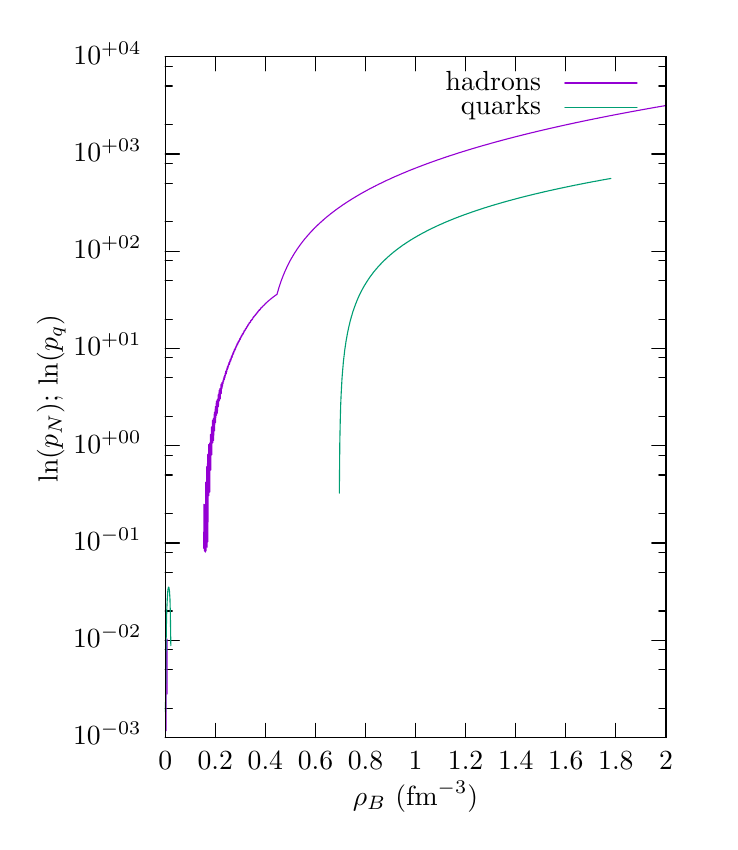
\begin{tikzpicture}[gnuplot]
%% generated with GNUPLOT 5.0p4 (Lua 5.2; terminal rev. 99, script rev. 100)
%% Thu Sep 29 16:33:19 2016
\path (0.000,0.000) rectangle (8.600,10.000);
\gpcolor{color=gp lt color border}
\gpsetlinetype{gp lt border}
\gpsetdashtype{gp dt solid}
\gpsetlinewidth{1.00}
\draw[gp path] (1.688,0.985)--(1.868,0.985);
\draw[gp path] (8.047,0.985)--(7.867,0.985);
\node[gp node right] at (1.504,0.985) {$10^{-03}$};
\draw[gp path] (1.688,1.357)--(1.778,1.357);
\draw[gp path] (8.047,1.357)--(7.957,1.357);
\draw[gp path] (1.688,1.848)--(1.778,1.848);
\draw[gp path] (8.047,1.848)--(7.957,1.848);
\draw[gp path] (1.688,2.100)--(1.778,2.100);
\draw[gp path] (8.047,2.100)--(7.957,2.100);
\draw[gp path] (1.688,2.220)--(1.868,2.220);
\draw[gp path] (8.047,2.220)--(7.867,2.220);
\node[gp node right] at (1.504,2.220) {$10^{-02}$};
\draw[gp path] (1.688,2.592)--(1.778,2.592);
\draw[gp path] (8.047,2.592)--(7.957,2.592);
\draw[gp path] (1.688,3.083)--(1.778,3.083);
\draw[gp path] (8.047,3.083)--(7.957,3.083);
\draw[gp path] (1.688,3.336)--(1.778,3.336);
\draw[gp path] (8.047,3.336)--(7.957,3.336);
\draw[gp path] (1.688,3.455)--(1.868,3.455);
\draw[gp path] (8.047,3.455)--(7.867,3.455);
\node[gp node right] at (1.504,3.455) {$10^{-01}$};
\draw[gp path] (1.688,3.827)--(1.778,3.827);
\draw[gp path] (8.047,3.827)--(7.957,3.827);
\draw[gp path] (1.688,4.319)--(1.778,4.319);
\draw[gp path] (8.047,4.319)--(7.957,4.319);
\draw[gp path] (1.688,4.571)--(1.778,4.571);
\draw[gp path] (8.047,4.571)--(7.957,4.571);
\draw[gp path] (1.688,4.690)--(1.868,4.690);
\draw[gp path] (8.047,4.690)--(7.867,4.690);
\node[gp node right] at (1.504,4.690) {$10^{+00}$};
\draw[gp path] (1.688,5.062)--(1.778,5.062);
\draw[gp path] (8.047,5.062)--(7.957,5.062);
\draw[gp path] (1.688,5.554)--(1.778,5.554);
\draw[gp path] (8.047,5.554)--(7.957,5.554);
\draw[gp path] (1.688,5.806)--(1.778,5.806);
\draw[gp path] (8.047,5.806)--(7.957,5.806);
\draw[gp path] (1.688,5.926)--(1.868,5.926);
\draw[gp path] (8.047,5.926)--(7.867,5.926);
\node[gp node right] at (1.504,5.926) {$10^{+01}$};
\draw[gp path] (1.688,6.297)--(1.778,6.297);
\draw[gp path] (8.047,6.297)--(7.957,6.297);
\draw[gp path] (1.688,6.789)--(1.778,6.789);
\draw[gp path] (8.047,6.789)--(7.957,6.789);
\draw[gp path] (1.688,7.041)--(1.778,7.041);
\draw[gp path] (8.047,7.041)--(7.957,7.041);
\draw[gp path] (1.688,7.161)--(1.868,7.161);
\draw[gp path] (8.047,7.161)--(7.867,7.161);
\node[gp node right] at (1.504,7.161) {$10^{+02}$};
\draw[gp path] (1.688,7.533)--(1.778,7.533);
\draw[gp path] (8.047,7.533)--(7.957,7.533);
\draw[gp path] (1.688,8.024)--(1.778,8.024);
\draw[gp path] (8.047,8.024)--(7.957,8.024);
\draw[gp path] (1.688,8.276)--(1.778,8.276);
\draw[gp path] (8.047,8.276)--(7.957,8.276);
\draw[gp path] (1.688,8.396)--(1.868,8.396);
\draw[gp path] (8.047,8.396)--(7.867,8.396);
\node[gp node right] at (1.504,8.396) {$10^{+03}$};
\draw[gp path] (1.688,8.768)--(1.778,8.768);
\draw[gp path] (8.047,8.768)--(7.957,8.768);
\draw[gp path] (1.688,9.259)--(1.778,9.259);
\draw[gp path] (8.047,9.259)--(7.957,9.259);
\draw[gp path] (1.688,9.511)--(1.778,9.511);
\draw[gp path] (8.047,9.511)--(7.957,9.511);
\draw[gp path] (1.688,9.631)--(1.868,9.631);
\draw[gp path] (8.047,9.631)--(7.867,9.631);
\node[gp node right] at (1.504,9.631) {$10^{+04}$};
\draw[gp path] (1.688,0.985)--(1.688,1.165);
\draw[gp path] (1.688,9.631)--(1.688,9.451);
\node[gp node center] at (1.688,0.677) {$0$};
\draw[gp path] (2.324,0.985)--(2.324,1.165);
\draw[gp path] (2.324,9.631)--(2.324,9.451);
\node[gp node center] at (2.324,0.677) {$0.2$};
\draw[gp path] (2.960,0.985)--(2.960,1.165);
\draw[gp path] (2.960,9.631)--(2.960,9.451);
\node[gp node center] at (2.960,0.677) {$0.4$};
\draw[gp path] (3.596,0.985)--(3.596,1.165);
\draw[gp path] (3.596,9.631)--(3.596,9.451);
\node[gp node center] at (3.596,0.677) {$0.6$};
\draw[gp path] (4.232,0.985)--(4.232,1.165);
\draw[gp path] (4.232,9.631)--(4.232,9.451);
\node[gp node center] at (4.232,0.677) {$0.8$};
\draw[gp path] (4.868,0.985)--(4.868,1.165);
\draw[gp path] (4.868,9.631)--(4.868,9.451);
\node[gp node center] at (4.868,0.677) {$1$};
\draw[gp path] (5.503,0.985)--(5.503,1.165);
\draw[gp path] (5.503,9.631)--(5.503,9.451);
\node[gp node center] at (5.503,0.677) {$1.2$};
\draw[gp path] (6.139,0.985)--(6.139,1.165);
\draw[gp path] (6.139,9.631)--(6.139,9.451);
\node[gp node center] at (6.139,0.677) {$1.4$};
\draw[gp path] (6.775,0.985)--(6.775,1.165);
\draw[gp path] (6.775,9.631)--(6.775,9.451);
\node[gp node center] at (6.775,0.677) {$1.6$};
\draw[gp path] (7.411,0.985)--(7.411,1.165);
\draw[gp path] (7.411,9.631)--(7.411,9.451);
\node[gp node center] at (7.411,0.677) {$1.8$};
\draw[gp path] (8.047,0.985)--(8.047,1.165);
\draw[gp path] (8.047,9.631)--(8.047,9.451);
\node[gp node center] at (8.047,0.677) {$2$};
\draw[gp path] (1.688,9.631)--(1.688,0.985)--(8.047,0.985)--(8.047,9.631)--cycle;
\node[gp node center,rotate=-270] at (0.246,5.308) {$\ln(p_N)$; $\ln(p_q)$};
\node[gp node center] at (4.867,0.215) {$\rho_B$ ($\rm{fm}^{-3}$)};
\node[gp node right] at (6.579,9.297) {hadrons};
\gpcolor{rgb color={0.580,0.000,0.827}}
\draw[gp path] (6.763,9.297)--(7.679,9.297);
\draw[gp path] (1.698,1.070)--(1.700,1.846)--(1.702,2.220);
\draw[gp path] (1.710,1.535)--(1.712,2.235);
\draw[gp path] (2.177,3.388)--(2.179,3.947);
\draw[gp path] (2.187,3.351)--(2.189,3.943);
\draw[gp path] (2.198,3.339)--(2.200,3.948)--(2.202,4.228);
\draw[gp path] (2.208,3.356)--(2.210,3.962)--(2.213,4.241)--(2.215,4.425);
\draw[gp path] (2.219,3.402)--(2.221,3.985)--(2.223,4.260)--(2.225,4.442)--(2.227,4.578)%
  --(2.229,3.471)--(2.232,4.017)--(2.234,4.284)--(2.236,4.462)--(2.238,4.597)--(2.240,4.705)%
  --(2.242,4.057)--(2.244,4.313)--(2.246,4.486)--(2.249,4.618)--(2.251,4.724)--(2.253,4.103)%
  --(2.255,4.346)--(2.257,4.513)--(2.259,4.642)--(2.261,4.746)--(2.263,4.834)--(2.266,4.383)%
  --(2.268,4.544)--(2.270,4.668)--(2.272,4.770)--(2.274,4.855)--(2.276,4.930)--(2.278,4.576)%
  --(2.280,4.696)--(2.282,4.795)--(2.285,4.879)--(2.287,4.952)--(2.289,5.016)--(2.291,4.727)%
  --(2.293,4.822)--(2.295,4.903)--(2.297,4.975)--(2.299,5.038)--(2.302,4.758)--(2.304,4.850)%
  --(2.306,4.929)--(2.308,4.999)--(2.310,5.060)--(2.312,5.116)--(2.314,4.880)--(2.316,4.957)%
  --(2.318,5.024)--(2.321,5.084)--(2.323,5.138)--(2.325,5.188)--(2.327,4.985)--(2.329,5.050)%
  --(2.331,5.108)--(2.333,5.161)--(2.335,5.210)--(2.338,5.255)--(2.340,5.077)--(2.342,5.134)%
  --(2.344,5.185)--(2.346,5.233)--(2.348,5.276)--(2.350,5.105)--(2.352,5.160)--(2.355,5.210)%
  --(2.357,5.256)--(2.359,5.299)--(2.361,5.338)--(2.363,5.186)--(2.365,5.235)--(2.367,5.280)%
  --(2.369,5.321)--(2.371,5.360)--(2.374,5.397)--(2.376,5.261)--(2.378,5.304)--(2.380,5.345)%
  --(2.382,5.383)--(2.384,5.418)--(2.386,5.287)--(2.388,5.329)--(2.391,5.368)--(2.393,5.405)%
  --(2.395,5.440)--(2.397,5.473)--(2.399,5.354)--(2.401,5.392)--(2.403,5.428)--(2.405,5.462)%
  --(2.408,5.494)--(2.410,5.420)--(2.412,5.454)--(2.414,5.487)--(2.416,5.449)--(2.418,5.482)%
  --(2.420,5.514)--(2.422,5.478)--(2.424,5.510)--(2.427,5.540)--(2.429,5.505)--(2.431,5.536)%
  --(2.433,5.565)--(2.435,5.532)--(2.437,5.562)--(2.439,5.529)--(2.441,5.559)--(2.444,5.587)%
  --(2.446,5.555)--(2.448,5.584)--(2.450,5.612)--(2.452,5.581)--(2.454,5.609)--(2.456,5.636)%
  --(2.458,5.607)--(2.460,5.633)--(2.463,5.604)--(2.465,5.631)--(2.467,5.657)--(2.469,5.629)%
  --(2.471,5.655)--(2.473,5.680)--(2.475,5.654)--(2.477,5.679)--(2.480,5.703)--(2.482,5.677)%
  --(2.484,5.702)--(2.486,5.676)--(2.488,5.701)--(2.490,5.724)--(2.492,5.700)--(2.494,5.723)%
  --(2.497,5.746)--(2.499,5.722)--(2.501,5.745)--(2.503,5.722)--(2.505,5.745)--(2.507,5.767)%
  --(2.509,5.744)--(2.511,5.767)--(2.513,5.788)--(2.516,5.767)--(2.518,5.788)--(2.520,5.766)%
  --(2.522,5.788)--(2.524,5.809)--(2.526,5.788)--(2.528,5.810)--(2.530,5.830)--(2.533,5.810)%
  --(2.535,5.830)--(2.537,5.810)--(2.539,5.831)--(2.541,5.851)--(2.543,5.831)--(2.545,5.851)%
  --(2.547,5.871)--(2.550,5.852)--(2.552,5.872)--(2.554,5.853)--(2.556,5.872)--(2.558,5.891)%
  --(2.560,5.873)--(2.562,5.892)--(2.564,5.911)--(2.566,5.894)--(2.569,5.912)--(2.571,5.895)%
  --(2.573,5.913)--(2.575,5.931)--(2.577,5.915)--(2.579,5.933)--(2.581,5.916)--(2.583,5.934)%
  --(2.586,5.952)--(2.588,5.936)--(2.590,5.953)--(2.592,5.970)--(2.594,5.955)--(2.596,5.972)%
  --(2.598,5.957)--(2.600,5.974)--(2.602,5.991)--(2.605,5.976)--(2.607,5.992)--(2.609,5.978)%
  --(2.611,5.995)--(2.613,6.011)--(2.615,5.997)--(2.617,6.013)--(2.619,5.999)--(2.622,6.015)%
  --(2.624,6.031)--(2.626,6.017)--(2.628,6.033)--(2.630,6.020)--(2.632,6.036)--(2.634,6.051)%
  --(2.636,6.038)--(2.639,6.053)--(2.641,6.041)--(2.643,6.056)--(2.645,6.071)--(2.647,6.059)%
  --(2.649,6.074)--(2.651,6.061)--(2.653,6.076)--(2.655,6.091)--(2.658,6.079)--(2.660,6.094)%
  --(2.662,6.082)--(2.664,6.097)--(2.666,6.111)--(2.668,6.100)--(2.670,6.114)--(2.672,6.103)%
  --(2.675,6.117)--(2.677,6.106)--(2.679,6.120)--(2.681,6.134)--(2.683,6.123)--(2.685,6.137)%
  --(2.687,6.127)--(2.689,6.141)--(2.691,6.154)--(2.694,6.144)--(2.696,6.157)--(2.698,6.147)%
  --(2.700,6.161)--(2.702,6.151)--(2.704,6.164)--(2.706,6.177)--(2.708,6.168)--(2.711,6.181)%
  --(2.713,6.171)--(2.715,6.185)--(2.717,6.175)--(2.719,6.188)--(2.721,6.201)--(2.723,6.192)%
  --(2.725,6.205)--(2.728,6.196)--(2.730,6.208)--(2.732,6.200)--(2.734,6.212)--(2.736,6.225)%
  --(2.738,6.216)--(2.740,6.229)--(2.742,6.220)--(2.744,6.233)--(2.747,6.224)--(2.749,6.237)%
  --(2.751,6.249)--(2.753,6.241)--(2.755,6.253)--(2.757,6.245)--(2.759,6.257)--(2.761,6.249)%
  --(2.764,6.261)--(2.766,6.253)--(2.768,6.265)--(2.770,6.258)--(2.772,6.270)--(2.774,6.281)%
  --(2.776,6.274)--(2.778,6.286)--(2.781,6.278)--(2.783,6.290)--(2.785,6.283)--(2.787,6.294)%
  --(2.789,6.288)--(2.791,6.299)--(2.793,6.292)--(2.795,6.304)--(2.797,6.297)--(2.800,6.308)%
  --(2.802,6.319)--(2.804,6.313)--(2.806,6.324)--(2.808,6.318)--(2.810,6.329)--(2.812,6.323)%
  --(2.814,6.334)--(2.817,6.328)--(2.819,6.338)--(2.821,6.333)--(2.823,6.343)--(2.825,6.338)%
  --(2.827,6.348)--(2.829,6.343)--(2.831,6.353)--(2.833,6.348)--(2.836,6.359)--(2.838,6.353)%
  --(2.840,6.364)--(2.842,6.358)--(2.844,6.369)--(2.846,6.364)--(2.848,6.374)--(2.850,6.369)%
  --(2.853,6.379)--(2.855,6.375)--(2.857,6.385)--(2.859,6.380)--(2.861,6.390)--(2.863,6.386)%
  --(2.865,6.396)--(2.867,6.391)--(2.870,6.401)--(2.872,6.397)--(2.874,6.407)--(2.876,6.403)%
  --(2.878,6.413)--(2.880,6.408)--(2.882,6.418)--(2.884,6.414)--(2.886,6.410)--(2.889,6.420)%
  --(2.891,6.416)--(2.893,6.426)--(2.895,6.422)--(2.897,6.432)--(2.899,6.428)--(2.901,6.438)%
  --(2.903,6.435)--(2.906,6.444)--(2.908,6.441)--(2.910,6.441)--(2.912,6.444)--(2.914,6.447)%
  --(2.916,6.450)--(2.918,6.453)--(2.920,6.456)--(2.923,6.453)--(2.925,6.457)--(2.927,6.460)%
  --(2.929,6.463)--(2.931,6.467)--(2.933,6.470)--(2.935,6.467)--(2.937,6.471)--(2.939,6.474)%
  --(2.942,6.477)--(2.944,6.475)--(2.946,6.478)--(2.948,6.482)--(2.950,6.485)--(2.952,6.489)%
  --(2.954,6.487)--(2.956,6.490)--(2.959,6.494)--(2.961,6.492)--(2.963,6.496)--(2.965,6.499)%
  --(2.967,6.503)--(2.969,6.501)--(2.971,6.505)--(2.973,6.509)--(2.975,6.507)--(2.978,6.511)%
  --(2.980,6.515)--(2.982,6.514)--(2.984,6.518)--(2.986,6.517)--(2.988,6.520)--(2.990,6.524)%
  --(2.992,6.524)--(2.995,6.528)--(2.997,6.527)--(2.999,6.531)--(3.001,6.530)--(3.003,6.534)%
  --(3.005,6.534)--(3.007,6.538)--(3.009,6.538)--(3.012,6.542)--(3.014,6.542)--(3.016,6.542)%
  --(3.018,6.547)--(3.020,6.547)--(3.022,6.551)--(3.024,6.551)--(3.026,6.552)--(3.028,6.556)%
  --(3.031,6.557)--(3.033,6.558)--(3.035,6.559)--(3.037,6.563)--(3.039,6.564)--(3.041,6.565)%
  --(3.043,6.567)--(3.045,6.568)--(3.048,6.569)--(3.050,6.571)--(3.052,6.572)--(3.054,6.574)%
  --(3.056,6.577)--(3.058,6.579)--(3.060,6.579)--(3.062,6.582)--(3.064,6.582)--(3.067,6.585)%
  --(3.069,6.586)--(3.071,6.587)--(3.073,6.589)--(3.075,6.591)--(3.077,6.593)--(3.079,6.594)%
  --(3.081,6.596)--(3.084,6.597)--(3.086,6.598)--(3.088,6.600)--(3.090,6.601)--(3.092,6.603)%
  --(3.094,6.604)--(3.096,6.606)--(3.098,6.607)--(3.101,6.609)--(3.103,6.610)--(3.105,6.611)%
  --(3.107,6.613)--(3.109,6.619)--(3.111,6.627)--(3.113,6.634)--(3.115,6.642)--(3.117,6.649)%
  --(3.120,6.657)--(3.122,6.664)--(3.124,6.671)--(3.126,6.678)--(3.128,6.685)--(3.130,6.692)%
  --(3.132,6.699)--(3.134,6.706)--(3.137,6.713)--(3.139,6.719)--(3.141,6.726)--(3.143,6.732)%
  --(3.145,6.739)--(3.147,6.745)--(3.149,6.751)--(3.151,6.757)--(3.154,6.764)--(3.156,6.770)%
  --(3.158,6.776)--(3.160,6.782)--(3.162,6.788)--(3.164,6.793)--(3.166,6.799)--(3.168,6.805)%
  --(3.170,6.811)--(3.173,6.816)--(3.175,6.822)--(3.177,6.827)--(3.179,6.833)--(3.181,6.838)%
  --(3.183,6.844)--(3.185,6.849)--(3.187,6.854)--(3.190,6.860)--(3.192,6.865)--(3.194,6.870)%
  --(3.196,6.875)--(3.198,6.880)--(3.200,6.885)--(3.202,6.890)--(3.204,6.895)--(3.206,6.900)%
  --(3.209,6.905)--(3.211,6.910)--(3.213,6.915)--(3.215,6.919)--(3.217,6.924)--(3.219,6.929)%
  --(3.221,6.933)--(3.223,6.938)--(3.226,6.943)--(3.228,6.947)--(3.230,6.952)--(3.232,6.956)%
  --(3.234,6.961)--(3.236,6.965)--(3.238,6.970)--(3.240,6.974)--(3.243,6.978)--(3.245,6.983)%
  --(3.247,6.987)--(3.249,6.991)--(3.251,6.995)--(3.253,7.000)--(3.255,7.004)--(3.257,7.008)%
  --(3.259,7.012)--(3.262,7.016)--(3.264,7.020)--(3.266,7.024)--(3.268,7.028)--(3.270,7.032)%
  --(3.272,7.036)--(3.274,7.040)--(3.276,7.044)--(3.279,7.048)--(3.281,7.052)--(3.283,7.056)%
  --(3.285,7.059)--(3.287,7.063)--(3.289,7.067)--(3.291,7.071)--(3.293,7.074)--(3.295,7.078)%
  --(3.298,7.082)--(3.300,7.085)--(3.302,7.089)--(3.304,7.093)--(3.306,7.096)--(3.308,7.100)%
  --(3.310,7.103)--(3.312,7.107)--(3.315,7.111)--(3.317,7.114)--(3.319,7.118)--(3.321,7.121)%
  --(3.323,7.124)--(3.325,7.128)--(3.327,7.131)--(3.329,7.135)--(3.332,7.138)--(3.334,7.141)%
  --(3.336,7.145)--(3.338,7.148)--(3.340,7.151)--(3.342,7.155)--(3.344,7.158)--(3.346,7.161)%
  --(3.348,7.165)--(3.351,7.168)--(3.353,7.171)--(3.355,7.174)--(3.357,7.177)--(3.359,7.181)%
  --(3.361,7.184)--(3.363,7.187)--(3.365,7.190)--(3.368,7.193)--(3.370,7.196)--(3.372,7.199)%
  --(3.374,7.202)--(3.376,7.205)--(3.378,7.208)--(3.380,7.212)--(3.382,7.215)--(3.385,7.218)%
  --(3.387,7.221)--(3.389,7.223)--(3.391,7.226)--(3.393,7.229)--(3.395,7.232)--(3.397,7.235)%
  --(3.399,7.238)--(3.401,7.241)--(3.404,7.244)--(3.406,7.247)--(3.408,7.250)--(3.410,7.253)%
  --(3.412,7.255)--(3.414,7.258)--(3.416,7.261)--(3.418,7.264)--(3.421,7.267)--(3.423,7.269)%
  --(3.425,7.272)--(3.427,7.275)--(3.429,7.278)--(3.431,7.280)--(3.433,7.283)--(3.435,7.286)%
  --(3.437,7.289)--(3.440,7.291)--(3.442,7.294)--(3.444,7.297)--(3.446,7.299)--(3.448,7.302)%
  --(3.450,7.305)--(3.452,7.307)--(3.454,7.310)--(3.457,7.312)--(3.459,7.315)--(3.461,7.318)%
  --(3.463,7.320)--(3.465,7.323)--(3.467,7.325)--(3.469,7.328)--(3.471,7.330)--(3.474,7.333)%
  --(3.476,7.335)--(3.478,7.338)--(3.480,7.340)--(3.482,7.343)--(3.484,7.345)--(3.486,7.348)%
  --(3.488,7.350)--(3.490,7.353)--(3.493,7.355)--(3.495,7.358)--(3.497,7.360)--(3.499,7.363)%
  --(3.501,7.365)--(3.503,7.367)--(3.505,7.370)--(3.507,7.372)--(3.510,7.375)--(3.512,7.377)%
  --(3.514,7.379)--(3.516,7.382)--(3.518,7.384)--(3.520,7.386)--(3.522,7.389)--(3.524,7.391)%
  --(3.527,7.393)--(3.529,7.396)--(3.531,7.398)--(3.533,7.400)--(3.535,7.403)--(3.537,7.405)%
  --(3.539,7.407)--(3.541,7.410)--(3.543,7.412)--(3.546,7.414)--(3.548,7.416)--(3.550,7.419)%
  --(3.552,7.421)--(3.554,7.423)--(3.556,7.425)--(3.558,7.427)--(3.560,7.430)--(3.563,7.432)%
  --(3.565,7.434)--(3.567,7.436)--(3.569,7.438)--(3.571,7.441)--(3.573,7.443)--(3.575,7.445)%
  --(3.577,7.447)--(3.579,7.449)--(3.582,7.451)--(3.584,7.454)--(3.586,7.456)--(3.588,7.458)%
  --(3.590,7.460)--(3.592,7.462)--(3.594,7.464)--(3.596,7.466)--(3.599,7.468)--(3.601,7.470)%
  --(3.603,7.473)--(3.605,7.475)--(3.607,7.477)--(3.609,7.479)--(3.611,7.481)--(3.613,7.483)%
  --(3.616,7.485)--(3.618,7.487)--(3.620,7.489)--(3.622,7.491)--(3.624,7.493)--(3.626,7.495)%
  --(3.628,7.497)--(3.630,7.499)--(3.632,7.501)--(3.635,7.503)--(3.637,7.505)--(3.639,7.507)%
  --(3.641,7.509)--(3.643,7.511)--(3.645,7.513)--(3.647,7.515)--(3.649,7.517)--(3.652,7.519)%
  --(3.654,7.521)--(3.656,7.523)--(3.658,7.525)--(3.660,7.527)--(3.662,7.528)--(3.664,7.530)%
  --(3.666,7.532)--(3.668,7.534)--(3.671,7.536)--(3.673,7.538)--(3.675,7.540)--(3.677,7.542)%
  --(3.679,7.544)--(3.681,7.546)--(3.683,7.548)--(3.685,7.549)--(3.688,7.551)--(3.690,7.553)%
  --(3.692,7.555)--(3.694,7.557)--(3.696,7.559)--(3.698,7.561)--(3.700,7.562)--(3.702,7.564)%
  --(3.705,7.566)--(3.707,7.568)--(3.709,7.570)--(3.711,7.572)--(3.713,7.573)--(3.715,7.575)%
  --(3.717,7.577)--(3.719,7.579)--(3.721,7.581)--(3.724,7.582)--(3.726,7.584)--(3.728,7.586)%
  --(3.730,7.588)--(3.732,7.589)--(3.734,7.591)--(3.736,7.593)--(3.738,7.595)--(3.741,7.597)%
  --(3.743,7.598)--(3.745,7.600)--(3.747,7.602)--(3.749,7.604)--(3.751,7.605)--(3.753,7.607)%
  --(3.755,7.609)--(3.758,7.610)--(3.760,7.612)--(3.762,7.614)--(3.764,7.616)--(3.766,7.617)%
  --(3.768,7.619)--(3.770,7.621)--(3.772,7.622)--(3.774,7.624)--(3.777,7.626)--(3.779,7.628)%
  --(3.781,7.629)--(3.783,7.631)--(3.785,7.633)--(3.787,7.634)--(3.789,7.636)--(3.791,7.638)%
  --(3.794,7.639)--(3.796,7.641)--(3.798,7.643)--(3.800,7.644)--(3.802,7.646)--(3.804,7.648)%
  --(3.806,7.649)--(3.808,7.651)--(3.810,7.652)--(3.813,7.654)--(3.815,7.656)--(3.817,7.657)%
  --(3.819,7.659)--(3.821,7.661)--(3.823,7.662)--(3.825,7.664)--(3.827,7.665)--(3.830,7.667)%
  --(3.832,7.669)--(3.834,7.670)--(3.836,7.672)--(3.838,7.673)--(3.840,7.675)--(3.842,7.677)%
  --(3.844,7.678)--(3.847,7.680)--(3.849,7.681)--(3.851,7.683)--(3.853,7.684)--(3.855,7.686)%
  --(3.857,7.688)--(3.859,7.689)--(3.861,7.691)--(3.863,7.692)--(3.866,7.694)--(3.868,7.695)%
  --(3.870,7.697)--(3.872,7.698)--(3.874,7.700)--(3.876,7.701)--(3.878,7.703)--(3.880,7.705)%
  --(3.883,7.706)--(3.885,7.708)--(3.887,7.709)--(3.889,7.711)--(3.891,7.712)--(3.893,7.714)%
  --(3.895,7.715)--(3.897,7.717)--(3.900,7.718)--(3.902,7.720)--(3.904,7.721)--(3.906,7.723)%
  --(3.908,7.724)--(3.910,7.726)--(3.912,7.727)--(3.914,7.729)--(3.916,7.730)--(3.919,7.732)%
  --(3.921,7.733)--(3.923,7.734)--(3.925,7.736)--(3.927,7.737)--(3.929,7.739)--(3.931,7.740)%
  --(3.933,7.742)--(3.936,7.743)--(3.938,7.745)--(3.940,7.746)--(3.942,7.748)--(3.944,7.749)%
  --(3.946,7.750)--(3.948,7.752)--(3.950,7.753)--(3.952,7.755)--(3.955,7.756)--(3.957,7.758)%
  --(3.959,7.759)--(3.961,7.760)--(3.963,7.762)--(3.965,7.763)--(3.967,7.765)--(3.969,7.766)%
  --(3.972,7.768)--(3.974,7.769)--(3.976,7.770)--(3.978,7.772)--(3.980,7.773)--(3.982,7.775)%
  --(3.984,7.776)--(3.986,7.777)--(3.989,7.779)--(3.991,7.780)--(3.993,7.782)--(3.995,7.783)%
  --(3.997,7.784)--(3.999,7.786)--(4.001,7.787)--(4.003,7.788)--(4.005,7.790)--(4.008,7.791)%
  --(4.010,7.793)--(4.012,7.794)--(4.014,7.795)--(4.016,7.797)--(4.018,7.798)--(4.020,7.799)%
  --(4.022,7.801)--(4.025,7.802)--(4.027,7.803)--(4.029,7.805)--(4.031,7.806)--(4.033,7.807)%
  --(4.035,7.809)--(4.037,7.810)--(4.039,7.811)--(4.041,7.813)--(4.044,7.814)--(4.046,7.815)%
  --(4.048,7.817)--(4.050,7.818)--(4.052,7.819)--(4.054,7.821)--(4.056,7.822)--(4.058,7.823)%
  --(4.061,7.825)--(4.063,7.826)--(4.065,7.827)--(4.067,7.829)--(4.069,7.830)--(4.071,7.831)%
  --(4.073,7.832)--(4.075,7.834)--(4.078,7.835)--(4.080,7.836)--(4.082,7.838)--(4.084,7.839)%
  --(4.086,7.840)--(4.088,7.842)--(4.090,7.843)--(4.092,7.844)--(4.094,7.845)--(4.097,7.847)%
  --(4.099,7.848)--(4.101,7.849)--(4.103,7.850)--(4.105,7.852)--(4.107,7.853)--(4.109,7.854)%
  --(4.111,7.856)--(4.114,7.857)--(4.116,7.858)--(4.118,7.859)--(4.120,7.861)--(4.122,7.862)%
  --(4.124,7.863)--(4.126,7.864)--(4.128,7.866)--(4.131,7.867)--(4.133,7.868)--(4.135,7.869)%
  --(4.137,7.871)--(4.139,7.872)--(4.141,7.873)--(4.143,7.874)--(4.145,7.876)--(4.147,7.877)%
  --(4.150,7.878)--(4.152,7.879)--(4.154,7.880)--(4.156,7.882)--(4.158,7.883)--(4.160,7.884)%
  --(4.162,7.885)--(4.164,7.887)--(4.167,7.888)--(4.169,7.889)--(4.171,7.890)--(4.173,7.891)%
  --(4.175,7.893)--(4.177,7.894)--(4.179,7.895)--(4.181,7.896)--(4.183,7.897)--(4.186,7.899)%
  --(4.188,7.900)--(4.190,7.901)--(4.192,7.902)--(4.194,7.903)--(4.196,7.905)--(4.198,7.906)%
  --(4.200,7.907)--(4.203,7.908)--(4.205,7.909)--(4.207,7.911)--(4.209,7.912)--(4.211,7.913)%
  --(4.213,7.914)--(4.215,7.915)--(4.217,7.916)--(4.220,7.918)--(4.222,7.919)--(4.224,7.920)%
  --(4.226,7.921)--(4.228,7.922)--(4.230,7.923)--(4.232,7.925)--(4.234,7.926)--(4.236,7.927)%
  --(4.239,7.928)--(4.241,7.929)--(4.243,7.930)--(4.245,7.932)--(4.247,7.933)--(4.249,7.934)%
  --(4.251,7.935)--(4.253,7.936)--(4.256,7.937)--(4.258,7.938)--(4.260,7.940)--(4.262,7.941)%
  --(4.264,7.942)--(4.266,7.943)--(4.268,7.944)--(4.270,7.945)--(4.273,7.946)--(4.275,7.948)%
  --(4.277,7.949)--(4.279,7.950)--(4.281,7.951)--(4.283,7.952)--(4.285,7.953)--(4.287,7.954)%
  --(4.289,7.955)--(4.292,7.957)--(4.294,7.958)--(4.296,7.959)--(4.298,7.960)--(4.300,7.961)%
  --(4.302,7.962)--(4.304,7.963)--(4.306,7.964)--(4.309,7.965)--(4.311,7.967)--(4.313,7.968)%
  --(4.315,7.969)--(4.317,7.970)--(4.319,7.971)--(4.321,7.972)--(4.323,7.973)--(4.325,7.974)%
  --(4.328,7.975)--(4.330,7.976)--(4.332,7.978)--(4.334,7.979)--(4.336,7.980)--(4.338,7.981)%
  --(4.340,7.982)--(4.342,7.983)--(4.345,7.984)--(4.347,7.985)--(4.349,7.986)--(4.351,7.987)%
  --(4.353,7.988)--(4.355,7.989)--(4.357,7.990)--(4.359,7.992)--(4.362,7.993)--(4.364,7.994)%
  --(4.366,7.995)--(4.368,7.996)--(4.370,7.997)--(4.372,7.998)--(4.374,7.999)--(4.376,8.000)%
  --(4.378,8.001)--(4.381,8.002)--(4.383,8.003)--(4.385,8.004)--(4.387,8.005)--(4.389,8.006)%
  --(4.391,8.008)--(4.393,8.009)--(4.395,8.010)--(4.398,8.011)--(4.400,8.012)--(4.402,8.013)%
  --(4.404,8.014)--(4.406,8.015)--(4.408,8.016)--(4.410,8.017)--(4.412,8.018)--(4.414,8.019)%
  --(4.417,8.020)--(4.419,8.021)--(4.421,8.022)--(4.423,8.023)--(4.425,8.024)--(4.427,8.025)%
  --(4.429,8.026)--(4.431,8.027)--(4.434,8.028)--(4.436,8.029)--(4.438,8.030)--(4.440,8.031)%
  --(4.442,8.032)--(4.444,8.033)--(4.446,8.034)--(4.448,8.035)--(4.451,8.037)--(4.453,8.038)%
  --(4.455,8.039)--(4.457,8.040)--(4.459,8.041)--(4.461,8.042)--(4.463,8.043)--(4.465,8.044)%
  --(4.467,8.045)--(4.470,8.046)--(4.472,8.047)--(4.474,8.048)--(4.476,8.049)--(4.478,8.050)%
  --(4.480,8.051)--(4.482,8.052)--(4.484,8.053)--(4.487,8.054)--(4.489,8.055)--(4.491,8.056)%
  --(4.493,8.057)--(4.495,8.058)--(4.497,8.059)--(4.499,8.060)--(4.501,8.061)--(4.504,8.062)%
  --(4.506,8.063)--(4.508,8.064)--(4.510,8.065)--(4.512,8.066)--(4.514,8.067)--(4.516,8.068)%
  --(4.518,8.068)--(4.520,8.069)--(4.523,8.070)--(4.525,8.071)--(4.527,8.072)--(4.529,8.073)%
  --(4.531,8.074)--(4.533,8.075)--(4.535,8.076)--(4.537,8.077)--(4.540,8.078)--(4.542,8.079)%
  --(4.544,8.080)--(4.546,8.081)--(4.548,8.082)--(4.550,8.083)--(4.552,8.084)--(4.554,8.085)%
  --(4.556,8.086)--(4.559,8.087)--(4.561,8.088)--(4.563,8.089)--(4.565,8.090)--(4.567,8.091)%
  --(4.569,8.092)--(4.571,8.093)--(4.573,8.094)--(4.576,8.095)--(4.578,8.096)--(4.580,8.096)%
  --(4.582,8.097)--(4.584,8.098)--(4.586,8.099)--(4.588,8.100)--(4.590,8.101)--(4.593,8.102)%
  --(4.595,8.103)--(4.597,8.104)--(4.599,8.105)--(4.601,8.106)--(4.603,8.107)--(4.605,8.108)%
  --(4.607,8.109)--(4.609,8.110)--(4.612,8.111)--(4.614,8.112)--(4.616,8.112)--(4.618,8.113)%
  --(4.620,8.114)--(4.622,8.115)--(4.624,8.116)--(4.626,8.117)--(4.629,8.118)--(4.631,8.119)%
  --(4.633,8.120)--(4.635,8.121)--(4.637,8.122)--(4.639,8.123)--(4.641,8.124)--(4.643,8.125)%
  --(4.646,8.125)--(4.648,8.126)--(4.650,8.127)--(4.652,8.128)--(4.654,8.129)--(4.656,8.130)%
  --(4.658,8.131)--(4.660,8.132)--(4.662,8.133)--(4.665,8.134)--(4.667,8.135)--(4.669,8.135)%
  --(4.671,8.136)--(4.673,8.137)--(4.675,8.138)--(4.677,8.139)--(4.679,8.140)--(4.682,8.141)%
  --(4.684,8.142)--(4.686,8.143)--(4.688,8.144)--(4.690,8.145)--(4.692,8.145)--(4.694,8.146)%
  --(4.696,8.147)--(4.698,8.148)--(4.701,8.149)--(4.703,8.150)--(4.705,8.151)--(4.707,8.152)%
  --(4.709,8.153)--(4.711,8.153)--(4.713,8.154)--(4.715,8.155)--(4.718,8.156)--(4.720,8.157)%
  --(4.722,8.158)--(4.724,8.159)--(4.726,8.160)--(4.728,8.161)--(4.730,8.161)--(4.732,8.162)%
  --(4.735,8.163)--(4.737,8.164)--(4.739,8.165)--(4.741,8.166)--(4.743,8.167)--(4.745,8.168)%
  --(4.747,8.168)--(4.749,8.169)--(4.751,8.170)--(4.754,8.171)--(4.756,8.172)--(4.758,8.173)%
  --(4.760,8.174)--(4.762,8.175)--(4.764,8.175)--(4.766,8.176)--(4.768,8.177)--(4.771,8.178)%
  --(4.773,8.179)--(4.775,8.180)--(4.777,8.181)--(4.779,8.182)--(4.781,8.182)--(4.783,8.183)%
  --(4.785,8.184)--(4.787,8.185)--(4.790,8.186)--(4.792,8.187)--(4.794,8.188)--(4.796,8.188)%
  --(4.798,8.189)--(4.800,8.190)--(4.802,8.191)--(4.804,8.192)--(4.807,8.193)--(4.809,8.194)%
  --(4.811,8.194)--(4.813,8.195)--(4.815,8.196)--(4.817,8.197)--(4.819,8.198)--(4.821,8.199)%
  --(4.824,8.199)--(4.826,8.200)--(4.828,8.201)--(4.830,8.202)--(4.832,8.203)--(4.834,8.204)%
  --(4.836,8.205)--(4.838,8.205)--(4.840,8.206)--(4.843,8.207)--(4.845,8.208)--(4.847,8.209)%
  --(4.849,8.210)--(4.851,8.210)--(4.853,8.211)--(4.855,8.212)--(4.857,8.213)--(4.860,8.214)%
  --(4.862,8.215)--(4.864,8.215)--(4.866,8.216)--(4.868,8.217)--(4.870,8.218)--(4.872,8.219)%
  --(4.874,8.220)--(4.877,8.220)--(4.879,8.221)--(4.881,8.222)--(4.883,8.223)--(4.885,8.224)%
  --(4.887,8.224)--(4.889,8.225)--(4.891,8.226)--(4.893,8.227)--(4.896,8.228)--(4.898,8.229)%
  --(4.900,8.229)--(4.902,8.230)--(4.904,8.231)--(4.906,8.232)--(4.908,8.233)--(4.910,8.233)%
  --(4.913,8.234)--(4.915,8.235)--(4.917,8.236)--(4.919,8.237)--(4.921,8.238)--(4.923,8.238)%
  --(4.925,8.239)--(4.927,8.240)--(4.929,8.241)--(4.932,8.242)--(4.934,8.242)--(4.936,8.243)%
  --(4.938,8.244)--(4.940,8.245)--(4.942,8.246)--(4.944,8.246)--(4.946,8.247)--(4.949,8.248)%
  --(4.951,8.249)--(4.953,8.250)--(4.955,8.250)--(4.957,8.251)--(4.959,8.252)--(4.961,8.253)%
  --(4.963,8.254)--(4.966,8.254)--(4.968,8.255)--(4.970,8.256)--(4.972,8.257)--(4.974,8.258)%
  --(4.976,8.258)--(4.978,8.259)--(4.980,8.260)--(4.982,8.261)--(4.985,8.262)--(4.987,8.262)%
  --(4.989,8.263)--(4.991,8.264)--(4.993,8.265)--(4.995,8.265)--(4.997,8.266)--(4.999,8.267)%
  --(5.002,8.268)--(5.004,8.269)--(5.006,8.269)--(5.008,8.270)--(5.010,8.271)--(5.012,8.272)%
  --(5.014,8.273)--(5.016,8.273)--(5.019,8.274)--(5.021,8.275)--(5.023,8.276)--(5.025,8.276)%
  --(5.027,8.277)--(5.029,8.278)--(5.031,8.279)--(5.033,8.279)--(5.035,8.280)--(5.038,8.281)%
  --(5.040,8.282)--(5.042,8.283)--(5.044,8.283)--(5.046,8.284)--(5.048,8.285)--(5.050,8.286)%
  --(5.052,8.286)--(5.055,8.287)--(5.057,8.288)--(5.059,8.289)--(5.061,8.290)--(5.063,8.290)%
  --(5.065,8.291)--(5.067,8.292)--(5.069,8.293)--(5.071,8.293)--(5.074,8.294)--(5.076,8.295)%
  --(5.078,8.296)--(5.080,8.296)--(5.082,8.297)--(5.084,8.298)--(5.086,8.299)--(5.088,8.299)%
  --(5.091,8.300)--(5.093,8.301)--(5.095,8.302)--(5.097,8.302)--(5.099,8.303)--(5.101,8.304)%
  --(5.103,8.305)--(5.105,8.305)--(5.108,8.306)--(5.110,8.307)--(5.112,8.308)--(5.114,8.308)%
  --(5.116,8.309)--(5.118,8.310)--(5.120,8.311)--(5.122,8.311)--(5.124,8.312)--(5.127,8.313)%
  --(5.129,8.314)--(5.131,8.314)--(5.133,8.315)--(5.135,8.316)--(5.137,8.317)--(5.139,8.317)%
  --(5.141,8.318)--(5.144,8.319)--(5.146,8.320)--(5.148,8.320)--(5.150,8.321)--(5.152,8.322)%
  --(5.154,8.323)--(5.156,8.323)--(5.158,8.324)--(5.160,8.325)--(5.163,8.326)--(5.165,8.326)%
  --(5.167,8.327)--(5.169,8.328)--(5.171,8.328)--(5.173,8.329)--(5.175,8.330)--(5.177,8.331)%
  --(5.180,8.331)--(5.182,8.332)--(5.184,8.333)--(5.186,8.334)--(5.188,8.334)--(5.190,8.335)%
  --(5.192,8.336)--(5.194,8.336)--(5.197,8.337)--(5.199,8.338)--(5.201,8.339)--(5.203,8.339)%
  --(5.205,8.340)--(5.207,8.341)--(5.209,8.342)--(5.211,8.342)--(5.213,8.343)--(5.216,8.344)%
  --(5.218,8.344)--(5.220,8.345)--(5.222,8.346)--(5.224,8.347)--(5.226,8.347)--(5.228,8.348)%
  --(5.230,8.349)--(5.233,8.349)--(5.235,8.350)--(5.237,8.351)--(5.239,8.352)--(5.241,8.352)%
  --(5.243,8.353)--(5.245,8.354)--(5.247,8.354)--(5.250,8.355)--(5.252,8.356)--(5.254,8.357)%
  --(5.256,8.357)--(5.258,8.358)--(5.260,8.359)--(5.262,8.359)--(5.264,8.360)--(5.266,8.361)%
  --(5.269,8.362)--(5.271,8.362)--(5.273,8.363)--(5.275,8.364)--(5.277,8.364)--(5.279,8.365)%
  --(5.281,8.366)--(5.283,8.367)--(5.286,8.367)--(5.288,8.368)--(5.290,8.369)--(5.292,8.369)%
  --(5.294,8.370)--(5.296,8.371)--(5.298,8.371)--(5.300,8.372)--(5.302,8.373)--(5.305,8.374)%
  --(5.307,8.374)--(5.309,8.375)--(5.311,8.376)--(5.313,8.376)--(5.315,8.377)--(5.317,8.378)%
  --(5.319,8.378)--(5.322,8.379)--(5.324,8.380)--(5.326,8.381)--(5.328,8.381)--(5.330,8.382)%
  --(5.332,8.383)--(5.334,8.383)--(5.336,8.384)--(5.339,8.385)--(5.341,8.385)--(5.343,8.386)%
  --(5.345,8.387)--(5.347,8.387)--(5.349,8.388)--(5.351,8.389)--(5.353,8.389)--(5.355,8.390)%
  --(5.358,8.391)--(5.360,8.392)--(5.362,8.392)--(5.364,8.393)--(5.366,8.394)--(5.368,8.394)%
  --(5.370,8.395)--(5.372,8.396)--(5.375,8.396)--(5.377,8.397)--(5.379,8.398)--(5.381,8.398)%
  --(5.383,8.399)--(5.385,8.400)--(5.387,8.400)--(5.389,8.401)--(5.392,8.402)--(5.394,8.402)%
  --(5.396,8.403)--(5.398,8.404)--(5.400,8.404)--(5.402,8.405)--(5.404,8.406)--(5.406,8.407)%
  --(5.408,8.407)--(5.411,8.408)--(5.413,8.409)--(5.415,8.409)--(5.417,8.410)--(5.419,8.411)%
  --(5.421,8.411)--(5.423,8.412)--(5.425,8.413)--(5.428,8.413)--(5.430,8.414)--(5.432,8.415)%
  --(5.434,8.415)--(5.436,8.416)--(5.438,8.417)--(5.440,8.417)--(5.442,8.418)--(5.444,8.419)%
  --(5.447,8.419)--(5.449,8.420)--(5.451,8.421)--(5.453,8.421)--(5.455,8.422)--(5.457,8.423)%
  --(5.459,8.423)--(5.461,8.424)--(5.464,8.425)--(5.466,8.425)--(5.468,8.426)--(5.470,8.427)%
  --(5.472,8.427)--(5.474,8.428)--(5.476,8.428)--(5.478,8.429)--(5.481,8.430)--(5.483,8.430)%
  --(5.485,8.431)--(5.487,8.432)--(5.489,8.432)--(5.491,8.433)--(5.493,8.434)--(5.495,8.434)%
  --(5.497,8.435)--(5.500,8.436)--(5.502,8.436)--(5.504,8.437)--(5.506,8.438)--(5.508,8.438)%
  --(5.510,8.439)--(5.512,8.440)--(5.514,8.440)--(5.517,8.441)--(5.519,8.442)--(5.521,8.442)%
  --(5.523,8.443)--(5.525,8.444)--(5.527,8.444)--(5.529,8.445)--(5.531,8.445)--(5.533,8.446)%
  --(5.536,8.447)--(5.538,8.447)--(5.540,8.448)--(5.542,8.449)--(5.544,8.449)--(5.546,8.450)%
  --(5.548,8.451)--(5.550,8.451)--(5.553,8.452)--(5.555,8.453)--(5.557,8.453)--(5.559,8.454)%
  --(5.561,8.454)--(5.563,8.455)--(5.565,8.456)--(5.567,8.456)--(5.570,8.457)--(5.572,8.458)%
  --(5.574,8.458)--(5.576,8.459)--(5.578,8.460)--(5.580,8.460)--(5.582,8.461)--(5.584,8.462)%
  --(5.586,8.462)--(5.589,8.463)--(5.591,8.463)--(5.593,8.464)--(5.595,8.465)--(5.597,8.465)%
  --(5.599,8.466)--(5.601,8.467)--(5.603,8.467)--(5.606,8.468)--(5.608,8.468)--(5.610,8.469)%
  --(5.612,8.470)--(5.614,8.470)--(5.616,8.471)--(5.618,8.472)--(5.620,8.472)--(5.623,8.473)%
  --(5.625,8.474)--(5.627,8.474)--(5.629,8.475)--(5.631,8.475)--(5.633,8.476)--(5.635,8.477)%
  --(5.637,8.477)--(5.639,8.478)--(5.642,8.479)--(5.644,8.479)--(5.646,8.480)--(5.648,8.480)%
  --(5.650,8.481)--(5.652,8.482)--(5.654,8.482)--(5.656,8.483)--(5.659,8.484)--(5.661,8.484)%
  --(5.663,8.485)--(5.665,8.485)--(5.667,8.486)--(5.669,8.487)--(5.671,8.487)--(5.673,8.488)%
  --(5.675,8.488)--(5.678,8.489)--(5.680,8.490)--(5.682,8.490)--(5.684,8.491)--(5.686,8.492)%
  --(5.688,8.492)--(5.690,8.493)--(5.692,8.493)--(5.695,8.494)--(5.697,8.495)--(5.699,8.495)%
  --(5.701,8.496)--(5.703,8.496)--(5.705,8.497)--(5.707,8.498)--(5.709,8.498)--(5.712,8.499)%
  --(5.714,8.500)--(5.716,8.500)--(5.718,8.501)--(5.720,8.501)--(5.722,8.502)--(5.724,8.503)%
  --(5.726,8.503)--(5.728,8.504)--(5.731,8.504)--(5.733,8.505)--(5.735,8.506)--(5.737,8.506)%
  --(5.739,8.507)--(5.741,8.507)--(5.743,8.508)--(5.745,8.509)--(5.748,8.509)--(5.750,8.510)%
  --(5.752,8.510)--(5.754,8.511)--(5.756,8.512)--(5.758,8.512)--(5.760,8.513)--(5.762,8.513)%
  --(5.764,8.514)--(5.767,8.515)--(5.769,8.515)--(5.771,8.516)--(5.773,8.516)--(5.775,8.517)%
  --(5.777,8.518)--(5.779,8.518)--(5.781,8.519)--(5.784,8.519)--(5.786,8.520)--(5.788,8.521)%
  --(5.790,8.521)--(5.792,8.522)--(5.794,8.522)--(5.796,8.523)--(5.798,8.524)--(5.801,8.524)%
  --(5.803,8.525)--(5.805,8.525)--(5.807,8.526)--(5.809,8.527)--(5.811,8.527)--(5.813,8.528)%
  --(5.815,8.528)--(5.817,8.529)--(5.820,8.530)--(5.822,8.530)--(5.824,8.531)--(5.826,8.531)%
  --(5.828,8.532)--(5.830,8.533)--(5.832,8.533)--(5.834,8.534)--(5.837,8.534)--(5.839,8.535)%
  --(5.841,8.536)--(5.843,8.536)--(5.845,8.537)--(5.847,8.537)--(5.849,8.538)--(5.851,8.538)%
  --(5.854,8.539)--(5.856,8.540)--(5.858,8.540)--(5.860,8.541)--(5.862,8.541)--(5.864,8.542)%
  --(5.866,8.543)--(5.868,8.543)--(5.870,8.544)--(5.873,8.544)--(5.875,8.545)--(5.877,8.545)%
  --(5.879,8.546)--(5.881,8.547)--(5.883,8.547)--(5.885,8.548)--(5.887,8.548)--(5.890,8.549)%
  --(5.892,8.550)--(5.894,8.550)--(5.896,8.551)--(5.898,8.551)--(5.900,8.552)--(5.902,8.552)%
  --(5.904,8.553)--(5.906,8.554)--(5.909,8.554)--(5.911,8.555)--(5.913,8.555)--(5.915,8.556)%
  --(5.917,8.556)--(5.919,8.557)--(5.921,8.558)--(5.923,8.558)--(5.926,8.559)--(5.928,8.559)%
  --(5.930,8.560)--(5.932,8.560)--(5.934,8.561)--(5.936,8.562)--(5.938,8.562)--(5.940,8.563)%
  --(5.943,8.563)--(5.945,8.564)--(5.947,8.564)--(5.949,8.565)--(5.951,8.566)--(5.953,8.566)%
  --(5.955,8.567)--(5.957,8.567)--(5.959,8.568)--(5.962,8.568)--(5.964,8.569)--(5.966,8.570)%
  --(5.968,8.570)--(5.970,8.571)--(5.972,8.571)--(5.974,8.572)--(5.976,8.572)--(5.979,8.573)%
  --(5.981,8.574)--(5.983,8.574)--(5.985,8.575)--(5.987,8.575)--(5.989,8.576)--(5.991,8.576)%
  --(5.993,8.577)--(5.996,8.578)--(5.998,8.578)--(6.000,8.579)--(6.002,8.579)--(6.004,8.580)%
  --(6.006,8.580)--(6.008,8.581)--(6.010,8.581)--(6.012,8.582)--(6.015,8.583)--(6.017,8.583)%
  --(6.019,8.584)--(6.021,8.584)--(6.023,8.585)--(6.025,8.585)--(6.027,8.586)--(6.029,8.587)%
  --(6.032,8.587)--(6.034,8.588)--(6.036,8.588)--(6.038,8.589)--(6.040,8.589)--(6.042,8.590)%
  --(6.044,8.590)--(6.046,8.591)--(6.048,8.592)--(6.051,8.592)--(6.053,8.593)--(6.055,8.593)%
  --(6.057,8.594)--(6.059,8.594)--(6.061,8.595)--(6.063,8.595)--(6.065,8.596)--(6.068,8.597)%
  --(6.070,8.597)--(6.072,8.598)--(6.074,8.598)--(6.076,8.599)--(6.078,8.599)--(6.080,8.600)%
  --(6.082,8.600)--(6.085,8.601)--(6.087,8.601)--(6.089,8.602)--(6.091,8.603)--(6.093,8.603)%
  --(6.095,8.604)--(6.097,8.604)--(6.099,8.605)--(6.101,8.605)--(6.104,8.606)--(6.106,8.606)%
  --(6.108,8.607)--(6.110,8.607)--(6.112,8.608)--(6.114,8.609)--(6.116,8.609)--(6.118,8.610)%
  --(6.121,8.610)--(6.123,8.611)--(6.125,8.611)--(6.127,8.612)--(6.129,8.612)--(6.131,8.613)%
  --(6.133,8.613)--(6.135,8.614)--(6.137,8.615)--(6.140,8.615)--(6.142,8.616)--(6.144,8.616)%
  --(6.146,8.617)--(6.148,8.617)--(6.150,8.618)--(6.152,8.618)--(6.154,8.619)--(6.157,8.619)%
  --(6.159,8.620)--(6.161,8.621)--(6.163,8.621)--(6.165,8.622)--(6.167,8.622)--(6.169,8.623)%
  --(6.171,8.623)--(6.174,8.624)--(6.176,8.624)--(6.178,8.625)--(6.180,8.625)--(6.182,8.626)%
  --(6.184,8.626)--(6.186,8.627)--(6.188,8.627)--(6.190,8.628)--(6.193,8.629)--(6.195,8.629)%
  --(6.197,8.630)--(6.199,8.630)--(6.201,8.631)--(6.203,8.631)--(6.205,8.632)--(6.207,8.632)%
  --(6.210,8.633)--(6.212,8.633)--(6.214,8.634)--(6.216,8.634)--(6.218,8.635)--(6.220,8.635)%
  --(6.222,8.636)--(6.224,8.637)--(6.227,8.637)--(6.229,8.638)--(6.231,8.638)--(6.233,8.639)%
  --(6.235,8.639)--(6.237,8.640)--(6.239,8.640)--(6.241,8.641)--(6.243,8.641)--(6.246,8.642)%
  --(6.248,8.642)--(6.250,8.643)--(6.252,8.643)--(6.254,8.644)--(6.256,8.644)--(6.258,8.645)%
  --(6.260,8.646)--(6.263,8.646)--(6.265,8.647)--(6.267,8.647)--(6.269,8.648)--(6.271,8.648)%
  --(6.273,8.649)--(6.275,8.649)--(6.277,8.650)--(6.279,8.650)--(6.282,8.651)--(6.284,8.651)%
  --(6.286,8.652)--(6.288,8.652)--(6.290,8.653)--(6.292,8.653)--(6.294,8.654)--(6.296,8.654)%
  --(6.299,8.655)--(6.301,8.655)--(6.303,8.656)--(6.305,8.656)--(6.307,8.657)--(6.309,8.658)%
  --(6.311,8.658)--(6.313,8.659)--(6.316,8.659)--(6.318,8.660)--(6.320,8.660)--(6.322,8.661)%
  --(6.324,8.661)--(6.326,8.662)--(6.328,8.662)--(6.330,8.663)--(6.332,8.663)--(6.335,8.664)%
  --(6.337,8.664)--(6.339,8.665)--(6.341,8.665)--(6.343,8.666)--(6.345,8.666)--(6.347,8.667)%
  --(6.349,8.667)--(6.352,8.668)--(6.354,8.668)--(6.356,8.669)--(6.358,8.669)--(6.360,8.670)%
  --(6.362,8.670)--(6.364,8.671)--(6.366,8.671)--(6.369,8.672)--(6.371,8.672)--(6.373,8.673)%
  --(6.375,8.673)--(6.377,8.674)--(6.379,8.674)--(6.381,8.675)--(6.383,8.675)--(6.385,8.676)%
  --(6.388,8.677)--(6.390,8.677)--(6.392,8.678)--(6.394,8.678)--(6.396,8.679)--(6.398,8.679)%
  --(6.400,8.680)--(6.402,8.680)--(6.405,8.681)--(6.407,8.681)--(6.409,8.682)--(6.411,8.682)%
  --(6.413,8.683)--(6.415,8.683)--(6.417,8.684)--(6.419,8.684)--(6.421,8.685)--(6.424,8.685)%
  --(6.426,8.686)--(6.428,8.686)--(6.430,8.687)--(6.432,8.687)--(6.434,8.688)--(6.436,8.688)%
  --(6.438,8.689)--(6.441,8.689)--(6.443,8.690)--(6.445,8.690)--(6.447,8.691)--(6.449,8.691)%
  --(6.451,8.692)--(6.453,8.692)--(6.455,8.693)--(6.458,8.693)--(6.460,8.694)--(6.462,8.694)%
  --(6.464,8.695)--(6.466,8.695)--(6.468,8.696)--(6.470,8.696)--(6.472,8.697)--(6.474,8.697)%
  --(6.477,8.698)--(6.479,8.698)--(6.481,8.699)--(6.483,8.699)--(6.485,8.700)--(6.487,8.700)%
  --(6.489,8.701)--(6.491,8.701)--(6.494,8.702)--(6.496,8.702)--(6.498,8.703)--(6.500,8.703)%
  --(6.502,8.704)--(6.504,8.704)--(6.506,8.705)--(6.508,8.705)--(6.510,8.706)--(6.513,8.706)%
  --(6.515,8.707)--(6.517,8.707)--(6.519,8.708)--(6.521,8.708)--(6.523,8.709)--(6.525,8.709)%
  --(6.527,8.710)--(6.530,8.710)--(6.532,8.711)--(6.534,8.711)--(6.536,8.711)--(6.538,8.712)%
  --(6.540,8.712)--(6.542,8.713)--(6.544,8.713)--(6.547,8.714)--(6.549,8.714)--(6.551,8.715)%
  --(6.553,8.715)--(6.555,8.716)--(6.557,8.716)--(6.559,8.717)--(6.561,8.717)--(6.563,8.718)%
  --(6.566,8.718)--(6.568,8.719)--(6.570,8.719)--(6.572,8.720)--(6.574,8.720)--(6.576,8.721)%
  --(6.578,8.721)--(6.580,8.722)--(6.583,8.722)--(6.585,8.723)--(6.587,8.723)--(6.589,8.724)%
  --(6.591,8.724)--(6.593,8.725)--(6.595,8.725)--(6.597,8.726)--(6.600,8.726)--(6.602,8.727)%
  --(6.604,8.727)--(6.606,8.728)--(6.608,8.728)--(6.610,8.729)--(6.612,8.729)--(6.614,8.729)%
  --(6.616,8.730)--(6.619,8.730)--(6.621,8.731)--(6.623,8.731)--(6.625,8.732)--(6.627,8.732)%
  --(6.629,8.733)--(6.631,8.733)--(6.633,8.734)--(6.636,8.734)--(6.638,8.735)--(6.640,8.735)%
  --(6.642,8.736)--(6.644,8.736)--(6.646,8.737)--(6.648,8.737)--(6.650,8.738)--(6.652,8.738)%
  --(6.655,8.739)--(6.657,8.739)--(6.659,8.740)--(6.661,8.740)--(6.663,8.741)--(6.665,8.741)%
  --(6.667,8.741)--(6.669,8.742)--(6.672,8.742)--(6.674,8.743)--(6.676,8.743)--(6.678,8.744)%
  --(6.680,8.744)--(6.682,8.745)--(6.684,8.745)--(6.686,8.746)--(6.689,8.746)--(6.691,8.747)%
  --(6.693,8.747)--(6.695,8.748)--(6.697,8.748)--(6.699,8.749)--(6.701,8.749)--(6.703,8.750)%
  --(6.705,8.750)--(6.708,8.750)--(6.710,8.751)--(6.712,8.751)--(6.714,8.752)--(6.716,8.752)%
  --(6.718,8.753)--(6.720,8.753)--(6.722,8.754)--(6.725,8.754)--(6.727,8.755)--(6.729,8.755)%
  --(6.731,8.756)--(6.733,8.756)--(6.735,8.757)--(6.737,8.757)--(6.739,8.758)--(6.742,8.758)%
  --(6.744,8.758)--(6.746,8.759)--(6.748,8.759)--(6.750,8.760)--(6.752,8.760)--(6.754,8.761)%
  --(6.756,8.761)--(6.758,8.762)--(6.761,8.762)--(6.763,8.763)--(6.765,8.763)--(6.767,8.764)%
  --(6.769,8.764)--(6.771,8.765)--(6.773,8.765)--(6.775,8.765)--(6.778,8.766)--(6.780,8.766)%
  --(6.782,8.767)--(6.784,8.767)--(6.786,8.768)--(6.788,8.768)--(6.790,8.769)--(6.792,8.769)%
  --(6.794,8.770)--(6.797,8.770)--(6.799,8.771)--(6.801,8.771)--(6.803,8.771)--(6.805,8.772)%
  --(6.807,8.772)--(6.809,8.773)--(6.811,8.773)--(6.814,8.774)--(6.816,8.774)--(6.818,8.775)%
  --(6.820,8.775)--(6.822,8.776)--(6.824,8.776)--(6.826,8.777)--(6.828,8.777)--(6.831,8.777)%
  --(6.833,8.778)--(6.835,8.778)--(6.837,8.779)--(6.839,8.779)--(6.841,8.780)--(6.843,8.780)%
  --(6.845,8.781)--(6.847,8.781)--(6.850,8.782)--(6.852,8.782)--(6.854,8.782)--(6.856,8.783)%
  --(6.858,8.783)--(6.860,8.784)--(6.862,8.784)--(6.864,8.785)--(6.867,8.785)--(6.869,8.786)%
  --(6.871,8.786)--(6.873,8.787)--(6.875,8.787)--(6.877,8.788)--(6.879,8.788)--(6.881,8.788)%
  --(6.883,8.789)--(6.886,8.789)--(6.888,8.790)--(6.890,8.790)--(6.892,8.791)--(6.894,8.791)%
  --(6.896,8.792)--(6.898,8.792)--(6.900,8.792)--(6.903,8.793)--(6.905,8.793)--(6.907,8.794)%
  --(6.909,8.794)--(6.911,8.795)--(6.913,8.795)--(6.915,8.796)--(6.917,8.796)--(6.920,8.797)%
  --(6.922,8.797)--(6.924,8.797)--(6.926,8.798)--(6.928,8.798)--(6.930,8.799)--(6.932,8.799)%
  --(6.934,8.800)--(6.936,8.800)--(6.939,8.801)--(6.941,8.801)--(6.943,8.801)--(6.945,8.802)%
  --(6.947,8.802)--(6.949,8.803)--(6.951,8.803)--(6.953,8.804)--(6.956,8.804)--(6.958,8.805)%
  --(6.960,8.805)--(6.962,8.806)--(6.964,8.806)--(6.966,8.806)--(6.968,8.807)--(6.970,8.807)%
  --(6.973,8.808)--(6.975,8.808)--(6.977,8.809)--(6.979,8.809)--(6.981,8.810)--(6.983,8.810)%
  --(6.985,8.810)--(6.987,8.811)--(6.989,8.811)--(6.992,8.812)--(6.994,8.812)--(6.996,8.813)%
  --(6.998,8.813)--(7.000,8.814)--(7.002,8.814)--(7.004,8.814)--(7.006,8.815)--(7.009,8.815)%
  --(7.011,8.816)--(7.013,8.816)--(7.015,8.817)--(7.017,8.817)--(7.019,8.817)--(7.021,8.818)%
  --(7.023,8.818)--(7.025,8.819)--(7.028,8.819)--(7.030,8.820)--(7.032,8.820)--(7.034,8.821)%
  --(7.036,8.821)--(7.038,8.821)--(7.040,8.822)--(7.042,8.822)--(7.045,8.823)--(7.047,8.823)%
  --(7.049,8.824)--(7.051,8.824)--(7.053,8.825)--(7.055,8.825)--(7.057,8.825)--(7.059,8.826)%
  --(7.062,8.826)--(7.064,8.827)--(7.066,8.827)--(7.068,8.828)--(7.070,8.828)--(7.072,8.828)%
  --(7.074,8.829)--(7.076,8.829)--(7.078,8.830)--(7.081,8.830)--(7.083,8.831)--(7.085,8.831)%
  --(7.087,8.832)--(7.089,8.832)--(7.091,8.832)--(7.093,8.833)--(7.095,8.833)--(7.098,8.834)%
  --(7.100,8.834)--(7.102,8.835)--(7.104,8.835)--(7.106,8.835)--(7.108,8.836)--(7.110,8.836)%
  --(7.112,8.837)--(7.115,8.837)--(7.117,8.838)--(7.119,8.838)--(7.121,8.838)--(7.123,8.839)%
  --(7.125,8.839)--(7.127,8.840)--(7.129,8.840)--(7.131,8.841)--(7.134,8.841)--(7.136,8.841)%
  --(7.138,8.842)--(7.140,8.842)--(7.142,8.843)--(7.144,8.843)--(7.146,8.844)--(7.148,8.844)%
  --(7.151,8.844)--(7.153,8.845)--(7.155,8.845)--(7.157,8.846)--(7.159,8.846)--(7.161,8.847)%
  --(7.163,8.847)--(7.165,8.847)--(7.167,8.848)--(7.170,8.848)--(7.172,8.849)--(7.174,8.849)%
  --(7.176,8.850)--(7.178,8.850)--(7.180,8.850)--(7.182,8.851)--(7.184,8.851)--(7.187,8.852)%
  --(7.189,8.852)--(7.191,8.853)--(7.193,8.853)--(7.195,8.853)--(7.197,8.854)--(7.199,8.854)%
  --(7.201,8.855)--(7.204,8.855)--(7.206,8.856)--(7.208,8.856)--(7.210,8.856)--(7.212,8.857)%
  --(7.214,8.857)--(7.216,8.858)--(7.218,8.858)--(7.220,8.859)--(7.223,8.859)--(7.225,8.859)%
  --(7.227,8.860)--(7.229,8.860)--(7.231,8.861)--(7.233,8.861)--(7.235,8.861)--(7.237,8.862)%
  --(7.240,8.862)--(7.242,8.863)--(7.244,8.863)--(7.246,8.864)--(7.248,8.864)--(7.250,8.864)%
  --(7.252,8.865)--(7.254,8.865)--(7.256,8.866)--(7.259,8.866)--(7.261,8.867)--(7.263,8.867)%
  --(7.265,8.867)--(7.267,8.868)--(7.269,8.868)--(7.271,8.869)--(7.273,8.869)--(7.276,8.869)%
  --(7.278,8.870)--(7.280,8.870)--(7.282,8.871)--(7.284,8.871)--(7.286,8.872)--(7.288,8.872)%
  --(7.290,8.872)--(7.293,8.873)--(7.295,8.873)--(7.297,8.874)--(7.299,8.874)--(7.301,8.874)%
  --(7.303,8.875)--(7.305,8.875)--(7.307,8.876)--(7.309,8.876)--(7.312,8.877)--(7.314,8.877)%
  --(7.316,8.877)--(7.318,8.878)--(7.320,8.878)--(7.322,8.879)--(7.324,8.879)--(7.326,8.879)%
  --(7.329,8.880)--(7.331,8.880)--(7.333,8.881)--(7.335,8.881)--(7.337,8.882)--(7.339,8.882)%
  --(7.341,8.882)--(7.343,8.883)--(7.346,8.883)--(7.348,8.884)--(7.350,8.884)--(7.352,8.884)%
  --(7.354,8.885)--(7.356,8.885)--(7.358,8.886)--(7.360,8.886)--(7.362,8.886)--(7.365,8.887)%
  --(7.367,8.887)--(7.369,8.888)--(7.371,8.888)--(7.373,8.889)--(7.375,8.889)--(7.377,8.889)%
  --(7.379,8.890)--(7.382,8.890)--(7.384,8.891)--(7.386,8.891)--(7.388,8.891)--(7.390,8.892)%
  --(7.392,8.892)--(7.394,8.893)--(7.396,8.893)--(7.398,8.893)--(7.401,8.894)--(7.403,8.894)%
  --(7.405,8.895)--(7.407,8.895)--(7.409,8.895)--(7.411,8.896)--(7.413,8.896)--(7.415,8.897)%
  --(7.418,8.897)--(7.420,8.898)--(7.422,8.898)--(7.424,8.898)--(7.426,8.899)--(7.428,8.899)%
  --(7.430,8.900)--(7.432,8.900)--(7.435,8.900)--(7.437,8.901)--(7.439,8.901)--(7.441,8.902)%
  --(7.443,8.902)--(7.445,8.902)--(7.447,8.903)--(7.449,8.903)--(7.451,8.904)--(7.454,8.904)%
  --(7.456,8.904)--(7.458,8.905)--(7.460,8.905)--(7.462,8.906)--(7.464,8.906)--(7.466,8.906)%
  --(7.468,8.907)--(7.471,8.907)--(7.473,8.908)--(7.475,8.908)--(7.477,8.908)--(7.479,8.909)%
  --(7.481,8.909)--(7.483,8.910)--(7.485,8.910)--(7.488,8.910)--(7.490,8.911)--(7.492,8.911)%
  --(7.494,8.912)--(7.496,8.912)--(7.498,8.912)--(7.500,8.913)--(7.502,8.913)--(7.504,8.914)%
  --(7.507,8.914)--(7.509,8.914)--(7.511,8.915)--(7.513,8.915)--(7.515,8.916)--(7.517,8.916)%
  --(7.519,8.916)--(7.521,8.917)--(7.524,8.917)--(7.526,8.918)--(7.528,8.918)--(7.530,8.918)%
  --(7.532,8.919)--(7.534,8.919)--(7.536,8.920)--(7.538,8.920)--(7.540,8.920)--(7.543,8.921)%
  --(7.545,8.921)--(7.547,8.922)--(7.549,8.922)--(7.551,8.922)--(7.553,8.923)--(7.555,8.923)%
  --(7.557,8.924)--(7.560,8.924)--(7.562,8.924)--(7.564,8.925)--(7.566,8.925)--(7.568,8.926)%
  --(7.570,8.926)--(7.572,8.926)--(7.574,8.927)--(7.577,8.927)--(7.579,8.928)--(7.581,8.928)%
  --(7.583,8.928)--(7.585,8.929)--(7.587,8.929)--(7.589,8.930)--(7.591,8.930)--(7.593,8.930)%
  --(7.596,8.931)--(7.598,8.931)--(7.600,8.932)--(7.602,8.932)--(7.604,8.932)--(7.606,8.933)%
  --(7.608,8.933)--(7.610,8.934)--(7.613,8.934)--(7.615,8.934)--(7.617,8.935)--(7.619,8.935)%
  --(7.621,8.935)--(7.623,8.936)--(7.625,8.936)--(7.627,8.937)--(7.629,8.937)--(7.632,8.937)%
  --(7.634,8.938)--(7.636,8.938)--(7.638,8.939)--(7.640,8.939)--(7.642,8.939)--(7.644,8.940)%
  --(7.646,8.940)--(7.649,8.941)--(7.651,8.941)--(7.653,8.941)--(7.655,8.942)--(7.657,8.942)%
  --(7.659,8.942)--(7.661,8.943)--(7.663,8.943)--(7.666,8.944)--(7.668,8.944)--(7.670,8.944)%
  --(7.672,8.945)--(7.674,8.945)--(7.676,8.946)--(7.678,8.946)--(7.680,8.946)--(7.682,8.947)%
  --(7.685,8.947)--(7.687,8.948)--(7.689,8.948)--(7.691,8.948)--(7.693,8.949)--(7.695,8.949)%
  --(7.697,8.949)--(7.699,8.950)--(7.702,8.950)--(7.704,8.951)--(7.706,8.951)--(7.708,8.951)%
  --(7.710,8.952)--(7.712,8.952)--(7.714,8.953)--(7.716,8.953)--(7.719,8.953)--(7.721,8.954)%
  --(7.723,8.954)--(7.725,8.954)--(7.727,8.955)--(7.729,8.955)--(7.731,8.956)--(7.733,8.956)%
  --(7.735,8.956)--(7.738,8.957)--(7.740,8.957)--(7.742,8.958)--(7.744,8.958)--(7.746,8.958)%
  --(7.748,8.959)--(7.750,8.959)--(7.752,8.959)--(7.755,8.960)--(7.757,8.960)--(7.759,8.961)%
  --(7.761,8.961)--(7.763,8.961)--(7.765,8.962)--(7.767,8.962)--(7.769,8.963)--(7.771,8.963)%
  --(7.774,8.963)--(7.776,8.964)--(7.778,8.964)--(7.780,8.964)--(7.782,8.965)--(7.784,8.965)%
  --(7.786,8.966)--(7.788,8.966)--(7.791,8.966)--(7.793,8.967)--(7.795,8.967)--(7.797,8.967)%
  --(7.799,8.968)--(7.801,8.968)--(7.803,8.969)--(7.805,8.969)--(7.808,8.969)--(7.810,8.970)%
  --(7.812,8.970)--(7.814,8.971)--(7.816,8.971)--(7.818,8.971)--(7.820,8.972)--(7.822,8.972)%
  --(7.824,8.972)--(7.827,8.973)--(7.829,8.973)--(7.831,8.974)--(7.833,8.974)--(7.835,8.974)%
  --(7.837,8.975)--(7.839,8.975)--(7.841,8.975)--(7.844,8.976)--(7.846,8.976)--(7.848,8.977)%
  --(7.850,8.977)--(7.852,8.977)--(7.854,8.978)--(7.856,8.978)--(7.858,8.978)--(7.861,8.979)%
  --(7.863,8.979)--(7.865,8.980)--(7.867,8.980)--(7.869,8.980)--(7.871,8.981)--(7.873,8.981)%
  --(7.875,8.981)--(7.877,8.982)--(7.880,8.982)--(7.882,8.983)--(7.884,8.983)--(7.886,8.983)%
  --(7.888,8.984)--(7.890,8.984)--(7.892,8.984)--(7.894,8.985)--(7.897,8.985)--(7.899,8.986)%
  --(7.901,8.986)--(7.903,8.986)--(7.905,8.987)--(7.907,8.987)--(7.909,8.987)--(7.911,8.988)%
  --(7.913,8.988)--(7.916,8.989)--(7.918,8.989)--(7.920,8.989)--(7.922,8.990)--(7.924,8.990)%
  --(7.926,8.990)--(7.928,8.991)--(7.930,8.991)--(7.933,8.991)--(7.935,8.992)--(7.937,8.992)%
  --(7.939,8.993)--(7.941,8.993)--(7.943,8.993)--(7.945,8.994)--(7.947,8.994)--(7.950,8.994)%
  --(7.952,8.995)--(7.954,8.995)--(7.956,8.996)--(7.958,8.996)--(7.960,8.996)--(7.962,8.997)%
  --(7.964,8.997)--(7.966,8.997)--(7.969,8.998)--(7.971,8.998)--(7.973,8.999)--(7.975,8.999)%
  --(7.977,8.999)--(7.979,9.000)--(7.981,9.000)--(7.983,9.000)--(7.986,9.001)--(7.988,9.001)%
  --(7.990,9.001)--(7.992,9.002)--(7.994,9.002)--(7.996,9.003)--(7.998,9.003)--(8.000,9.003)%
  --(8.002,9.004)--(8.005,9.004)--(8.007,9.004)--(8.009,9.005)--(8.011,9.005)--(8.013,9.005)%
  --(8.015,9.006)--(8.017,9.006)--(8.019,9.007)--(8.022,9.007)--(8.024,9.007)--(8.026,9.008)%
  --(8.028,9.008)--(8.030,9.008)--(8.032,9.009)--(8.034,9.009)--(8.036,9.009)--(8.039,9.010)%
  --(8.041,9.010)--(8.043,9.011)--(8.045,9.011)--(8.047,9.011);
\gpcolor{color=gp lt color border}
\node[gp node right] at (6.579,8.989) {quarks};
\gpcolor{rgb color={0.000,0.620,0.451}}
\draw[gp path] (6.763,8.989)--(7.679,8.989);
\draw[gp path] (1.691,1.309)--(1.697,2.079)--(1.703,2.419)--(1.708,2.619)--(1.714,2.747)%
  --(1.719,2.830)--(1.725,2.878)--(1.731,2.896)--(1.736,2.884)--(1.742,2.838)--(1.748,2.746)%
  --(1.753,2.550)--(1.759,2.153);
\draw[gp path] (3.899,4.088)--(3.905,4.737)--(3.911,5.022)--(3.916,5.207)--(3.922,5.345)%
  --(3.928,5.455)--(3.933,5.546)--(3.939,5.623)--(3.945,5.691)--(3.950,5.752)--(3.956,5.806)%
  --(3.962,5.855)--(3.967,5.901)--(3.973,5.942)--(3.979,5.981)--(3.984,6.017)--(3.990,6.051)%
  --(3.996,6.083)--(4.001,6.113)--(4.007,6.142)--(4.013,6.169)--(4.018,6.195)--(4.024,6.220)%
  --(4.030,6.243)--(4.035,6.266)--(4.041,6.288)--(4.047,6.309)--(4.052,6.329)--(4.058,6.348)%
  --(4.064,6.367)--(4.069,6.385)--(4.075,6.403)--(4.081,6.420)--(4.086,6.436)--(4.092,6.452)%
  --(4.098,6.468)--(4.103,6.483)--(4.109,6.498)--(4.115,6.512)--(4.120,6.526)--(4.126,6.540)%
  --(4.131,6.553)--(4.137,6.566)--(4.143,6.579)--(4.148,6.591)--(4.154,6.603)--(4.160,6.615)%
  --(4.165,6.627)--(4.171,6.638)--(4.177,6.649)--(4.182,6.660)--(4.188,6.671)--(4.194,6.682)%
  --(4.199,6.692)--(4.205,6.702)--(4.211,6.712)--(4.216,6.722)--(4.222,6.732)--(4.228,6.741)%
  --(4.233,6.750)--(4.239,6.759)--(4.245,6.768)--(4.250,6.777)--(4.256,6.786)--(4.262,6.795)%
  --(4.267,6.803)--(4.273,6.811)--(4.279,6.820)--(4.284,6.828)--(4.290,6.836)--(4.296,6.844)%
  --(4.301,6.851)--(4.307,6.859)--(4.313,6.867)--(4.318,6.874)--(4.324,6.882)--(4.330,6.889)%
  --(4.335,6.896)--(4.341,6.903)--(4.347,6.910)--(4.352,6.917)--(4.358,6.924)--(4.364,6.931)%
  --(4.369,6.937)--(4.375,6.944)--(4.381,6.950)--(4.386,6.957)--(4.392,6.963)--(4.398,6.969)%
  --(4.403,6.976)--(4.409,6.982)--(4.415,6.988)--(4.420,6.994)--(4.426,7.000)--(4.432,7.006)%
  --(4.437,7.012)--(4.443,7.018)--(4.449,7.023)--(4.454,7.029)--(4.460,7.035)--(4.466,7.040)%
  --(4.471,7.046)--(4.477,7.051)--(4.483,7.057)--(4.488,7.062)--(4.494,7.067)--(4.500,7.072)%
  --(4.505,7.078)--(4.511,7.083)--(4.517,7.088)--(4.522,7.093)--(4.528,7.098)--(4.533,7.103)%
  --(4.539,7.108)--(4.545,7.113)--(4.550,7.118)--(4.556,7.123)--(4.562,7.127)--(4.567,7.132)%
  --(4.573,7.137)--(4.579,7.141)--(4.584,7.146)--(4.590,7.151)--(4.596,7.155)--(4.601,7.160)%
  --(4.607,7.164)--(4.613,7.169)--(4.618,7.173)--(4.624,7.177)--(4.630,7.182)--(4.635,7.186)%
  --(4.641,7.190)--(4.647,7.195)--(4.652,7.199)--(4.658,7.203)--(4.664,7.207)--(4.669,7.211)%
  --(4.675,7.216)--(4.681,7.220)--(4.686,7.224)--(4.692,7.228)--(4.698,7.232)--(4.703,7.236)%
  --(4.709,7.240)--(4.715,7.244)--(4.720,7.247)--(4.726,7.251)--(4.732,7.255)--(4.737,7.259)%
  --(4.743,7.263)--(4.749,7.266)--(4.754,7.270)--(4.760,7.274)--(4.766,7.278)--(4.771,7.281)%
  --(4.777,7.285)--(4.783,7.289)--(4.788,7.292)--(4.794,7.296)--(4.800,7.299)--(4.805,7.303)%
  --(4.811,7.306)--(4.817,7.310)--(4.822,7.313)--(4.828,7.317)--(4.834,7.320)--(4.839,7.324)%
  --(4.845,7.327)--(4.851,7.330)--(4.856,7.334)--(4.862,7.337)--(4.868,7.340)--(4.873,7.344)%
  --(4.879,7.347)--(4.885,7.350)--(4.890,7.354)--(4.896,7.357)--(4.902,7.360)--(4.907,7.363)%
  --(4.913,7.366)--(4.919,7.370)--(4.924,7.373)--(4.930,7.376)--(4.936,7.379)--(4.941,7.382)%
  --(4.947,7.385)--(4.952,7.388)--(4.958,7.391)--(4.964,7.394)--(4.969,7.397)--(4.975,7.400)%
  --(4.981,7.403)--(4.986,7.406)--(4.992,7.409)--(4.998,7.412)--(5.003,7.415)--(5.009,7.418)%
  --(5.015,7.421)--(5.020,7.424)--(5.026,7.427)--(5.032,7.429)--(5.037,7.432)--(5.043,7.435)%
  --(5.049,7.438)--(5.054,7.441)--(5.060,7.444)--(5.066,7.446)--(5.071,7.449)--(5.077,7.452)%
  --(5.083,7.455)--(5.088,7.457)--(5.094,7.460)--(5.100,7.463)--(5.105,7.465)--(5.111,7.468)%
  --(5.117,7.471)--(5.122,7.473)--(5.128,7.476)--(5.134,7.479)--(5.139,7.481)--(5.145,7.484)%
  --(5.151,7.487)--(5.156,7.489)--(5.162,7.492)--(5.168,7.494)--(5.173,7.497)--(5.179,7.499)%
  --(5.185,7.502)--(5.190,7.504)--(5.196,7.507)--(5.202,7.509)--(5.207,7.512)--(5.213,7.514)%
  --(5.219,7.517)--(5.224,7.519)--(5.230,7.522)--(5.236,7.524)--(5.241,7.527)--(5.247,7.529)%
  --(5.253,7.532)--(5.258,7.534)--(5.264,7.536)--(5.270,7.539)--(5.275,7.541)--(5.281,7.543)%
  --(5.287,7.546)--(5.292,7.548)--(5.298,7.550)--(5.304,7.553)--(5.309,7.555)--(5.315,7.557)%
  --(5.321,7.560)--(5.326,7.562)--(5.332,7.564)--(5.338,7.567)--(5.343,7.569)--(5.349,7.571)%
  --(5.354,7.573)--(5.360,7.576)--(5.366,7.578)--(5.371,7.580)--(5.377,7.582)--(5.383,7.585)%
  --(5.388,7.587)--(5.394,7.589)--(5.400,7.591)--(5.405,7.593)--(5.411,7.595)--(5.417,7.598)%
  --(5.422,7.600)--(5.428,7.602)--(5.434,7.604)--(5.439,7.606)--(5.445,7.608)--(5.451,7.610)%
  --(5.456,7.613)--(5.462,7.615)--(5.468,7.617)--(5.473,7.619)--(5.479,7.621)--(5.485,7.623)%
  --(5.490,7.625)--(5.496,7.627)--(5.502,7.629)--(5.507,7.631)--(5.513,7.633)--(5.519,7.635)%
  --(5.524,7.637)--(5.530,7.639)--(5.536,7.641)--(5.541,7.643)--(5.547,7.645)--(5.553,7.647)%
  --(5.558,7.649)--(5.564,7.651)--(5.570,7.653)--(5.575,7.655)--(5.581,7.657)--(5.587,7.659)%
  --(5.592,7.661)--(5.598,7.663)--(5.604,7.665)--(5.609,7.667)--(5.615,7.669)--(5.621,7.671)%
  --(5.626,7.673)--(5.632,7.675)--(5.638,7.677)--(5.643,7.679)--(5.649,7.680)--(5.655,7.682)%
  --(5.660,7.684)--(5.666,7.686)--(5.672,7.688)--(5.677,7.690)--(5.683,7.692)--(5.689,7.694)%
  --(5.694,7.695)--(5.700,7.697)--(5.706,7.699)--(5.711,7.701)--(5.717,7.703)--(5.723,7.705)%
  --(5.728,7.706)--(5.734,7.708)--(5.740,7.710)--(5.745,7.712)--(5.751,7.714)--(5.756,7.715)%
  --(5.762,7.717)--(5.768,7.719)--(5.773,7.721)--(5.779,7.722)--(5.785,7.724)--(5.790,7.726)%
  --(5.796,7.728)--(5.802,7.729)--(5.807,7.731)--(5.813,7.733)--(5.819,7.735)--(5.824,7.736)%
  --(5.830,7.738)--(5.836,7.740)--(5.841,7.742)--(5.847,7.743)--(5.853,7.745)--(5.858,7.747)%
  --(5.864,7.748)--(5.870,7.750)--(5.875,7.752)--(5.881,7.753)--(5.887,7.755)--(5.892,7.757)%
  --(5.898,7.759)--(5.904,7.760)--(5.909,7.762)--(5.915,7.763)--(5.921,7.765)--(5.926,7.767)%
  --(5.932,7.768)--(5.938,7.770)--(5.943,7.772)--(5.949,7.773)--(5.955,7.775)--(5.960,7.777)%
  --(5.966,7.778)--(5.972,7.780)--(5.977,7.781)--(5.983,7.783)--(5.989,7.785)--(5.994,7.786)%
  --(6.000,7.788)--(6.006,7.789)--(6.011,7.791)--(6.017,7.793)--(6.023,7.794)--(6.028,7.796)%
  --(6.034,7.797)--(6.040,7.799)--(6.045,7.800)--(6.051,7.802)--(6.057,7.804)--(6.062,7.805)%
  --(6.068,7.807)--(6.074,7.808)--(6.079,7.810)--(6.085,7.811)--(6.091,7.813)--(6.096,7.814)%
  --(6.102,7.816)--(6.108,7.817)--(6.113,7.819)--(6.119,7.820)--(6.125,7.822)--(6.130,7.823)%
  --(6.136,7.825)--(6.142,7.826)--(6.147,7.828)--(6.153,7.829)--(6.158,7.831)--(6.164,7.832)%
  --(6.170,7.834)--(6.175,7.835)--(6.181,7.837)--(6.187,7.838)--(6.192,7.840)--(6.198,7.841)%
  --(6.204,7.843)--(6.209,7.844)--(6.215,7.846)--(6.221,7.847)--(6.226,7.848)--(6.232,7.850)%
  --(6.238,7.851)--(6.243,7.853)--(6.249,7.854)--(6.255,7.856)--(6.260,7.857)--(6.266,7.859)%
  --(6.272,7.860)--(6.277,7.861)--(6.283,7.863)--(6.289,7.864)--(6.294,7.866)--(6.300,7.867)%
  --(6.306,7.868)--(6.311,7.870)--(6.317,7.871)--(6.323,7.873)--(6.328,7.874)--(6.334,7.875)%
  --(6.340,7.877)--(6.345,7.878)--(6.351,7.880)--(6.357,7.881)--(6.362,7.882)--(6.368,7.884)%
  --(6.374,7.885)--(6.379,7.886)--(6.385,7.888)--(6.391,7.889)--(6.396,7.890)--(6.402,7.892)%
  --(6.408,7.893)--(6.413,7.894)--(6.419,7.896)--(6.425,7.897)--(6.430,7.898)--(6.436,7.900)%
  --(6.442,7.901)--(6.447,7.902)--(6.453,7.904)--(6.459,7.905)--(6.464,7.906)--(6.470,7.908)%
  --(6.476,7.909)--(6.481,7.910)--(6.487,7.912)--(6.493,7.913)--(6.498,7.914)--(6.504,7.916)%
  --(6.510,7.917)--(6.515,7.918)--(6.521,7.920)--(6.527,7.921)--(6.532,7.922)--(6.538,7.923)%
  --(6.544,7.925)--(6.549,7.926)--(6.555,7.927)--(6.560,7.929)--(6.566,7.930)--(6.572,7.931)%
  --(6.577,7.932)--(6.583,7.934)--(6.589,7.935)--(6.594,7.936)--(6.600,7.937)--(6.606,7.939)%
  --(6.611,7.940)--(6.617,7.941)--(6.623,7.942)--(6.628,7.944)--(6.634,7.945)--(6.640,7.946)%
  --(6.645,7.947)--(6.651,7.949)--(6.657,7.950)--(6.662,7.951)--(6.668,7.952)--(6.674,7.954)%
  --(6.679,7.955)--(6.685,7.956)--(6.691,7.957)--(6.696,7.958)--(6.702,7.960)--(6.708,7.961)%
  --(6.713,7.962)--(6.719,7.963)--(6.725,7.964)--(6.730,7.966)--(6.736,7.967)--(6.742,7.968)%
  --(6.747,7.969)--(6.753,7.970)--(6.759,7.972)--(6.764,7.973)--(6.770,7.974)--(6.776,7.975)%
  --(6.781,7.976)--(6.787,7.978)--(6.793,7.979)--(6.798,7.980)--(6.804,7.981)--(6.810,7.982)%
  --(6.815,7.983)--(6.821,7.985)--(6.827,7.986)--(6.832,7.987)--(6.838,7.988)--(6.844,7.989)%
  --(6.849,7.990)--(6.855,7.992)--(6.861,7.993)--(6.866,7.994)--(6.872,7.995)--(6.878,7.996)%
  --(6.883,7.997)--(6.889,7.999)--(6.895,8.000)--(6.900,8.001)--(6.906,8.002)--(6.912,8.003)%
  --(6.917,8.004)--(6.923,8.005)--(6.929,8.006)--(6.934,8.008)--(6.940,8.009)--(6.946,8.010)%
  --(6.951,8.011)--(6.957,8.012)--(6.962,8.013)--(6.968,8.014)--(6.974,8.015)--(6.979,8.017)%
  --(6.985,8.018)--(6.991,8.019)--(6.996,8.020)--(7.002,8.021)--(7.008,8.022)--(7.013,8.023)%
  --(7.019,8.024)--(7.025,8.025)--(7.030,8.027)--(7.036,8.028)--(7.042,8.029)--(7.047,8.030)%
  --(7.053,8.031)--(7.059,8.032)--(7.064,8.033)--(7.070,8.034)--(7.076,8.035)--(7.081,8.036)%
  --(7.087,8.037)--(7.093,8.038)--(7.098,8.040)--(7.104,8.041)--(7.110,8.042)--(7.115,8.043)%
  --(7.121,8.044)--(7.127,8.045)--(7.132,8.046)--(7.138,8.047)--(7.144,8.048)--(7.149,8.049)%
  --(7.155,8.050)--(7.161,8.051)--(7.166,8.052)--(7.172,8.053)--(7.178,8.054)--(7.183,8.055)%
  --(7.189,8.056)--(7.195,8.058)--(7.200,8.059)--(7.206,8.060)--(7.212,8.061)--(7.217,8.062)%
  --(7.223,8.063)--(7.229,8.064)--(7.234,8.065)--(7.240,8.066)--(7.246,8.067)--(7.251,8.068)%
  --(7.257,8.069)--(7.263,8.070)--(7.268,8.071)--(7.274,8.072)--(7.280,8.073)--(7.285,8.074)%
  --(7.291,8.075)--(7.297,8.076)--(7.302,8.077)--(7.308,8.078)--(7.314,8.079)--(7.319,8.080)%
  --(7.325,8.081)--(7.331,8.082)--(7.336,8.083)--(7.342,8.084)--(7.348,8.085);
\gpcolor{color=gp lt color border}
\draw[gp path] (1.688,9.631)--(1.688,0.985)--(8.047,0.985)--(8.047,9.631)--cycle;
%% coordinates of the plot area
\gpdefrectangularnode{gp plot 1}{\pgfpoint{1.688cm}{0.985cm}}{\pgfpoint{8.047cm}{9.631cm}}
\end{tikzpicture}
%% gnuplot variables

	\caption{Buballa\_3-eNJL2OmegaRho1}
\end{figure}

%\begin{figure}[!htpb]
%\includegraphics[width=\linewidth]{graph/Buballa_1-eNJL1-quark-hadron_phase_transition.pdf}
%\caption{Teste.}
%\end{figure}

%
%%
%%%
%%%% Back Matter
%%%
%%
%

%\begin{acknowledgments}
% Lorem ipsum.
%\end{acknowledgments}

%%%

%\appendix
%\section{Appendix title}

%%%

\bibliography{references}

%%%%%%%%%%%%%%
%%%%%%%%%%%%%%
%%%%%%%%%%%%%%
\end{document}
%%%%%%%%%%%%%%
%%%%%%%%%%%%%%
%%%%%%%%%%%%%%
